%
% ---------------------------------------------------------------------------------------
% VALOR T2K numu disappearance analysis, Run1+2+3
% ---------------------------------------------------------------------------------------
%

\documentclass[final]{elsarticle}

\usepackage[margin=2.50cm]{geometry}  % tweak margins
%\usepackage{draftcopy}                % uncomment to print a "DRAFT-COPY" in background
\usepackage{graphicx}                 % if you want to include PostScript figures
\usepackage[figuresright]{rotating}   % if you have landscape tables
\usepackage{multirow}                 % fancy tables
\usepackage[toc,page]{appendix}       % appendix
\usepackage{lineno}                   % for printing the line numbers
\usepackage{natbib}                   % for building bibliography with \cite{}
\usepackage{setspace}
\usepackage{times}
\usepackage{afterpage}
\usepackage{float}
\usepackage{subfigure}
\usepackage{longtable}
\usepackage{color} 
\usepackage{rotate}                   % rotate text in tables
\usepackage{amsfonts}                 % extra symbols
\usepackage{amsmath}                 
%\usepackage{floatpag}                 % \thisfloatpagestyle{empty}, to suppress page numbers
\usepackage{lmodern}
\usepackage[breaklinks=true,hyperfigures=true]{hyperref} % make contents and references links, but do not colour them

% use to fix date
% \def \today { February 1st, 2009 }
% put your own definitions here:
\newcommand{\ck}{$\checkmark$}
\newcommand{\ttbs}{\char'134}
%\newcommand{\AmS}{{\protect\the\textfont2
%  A\kern-.1667em\lower.5ex\hbox{M}\kern-.125emS}}
% add words to TeX's hyphenation exception list
%\hyphenation{author another created financial paper re-commend-ed Post-Script}

% By default, LaTeX doesn't like to fill more than 0.7 of a text page with tables and graphics, 
% nor does it like too many figures per page. This behaviour can be changed:
\renewcommand\floatpagefraction{.9}
\renewcommand\topfraction{.9}
\renewcommand\bottomfraction{.9}
\renewcommand\textfraction{.1}   
\setcounter{totalnumber}{50}
\setcounter{topnumber}{50}
\setcounter{bottomnumber}{50}

\linenumbers
\bibliographystyle{elsart-num}


%define new fonts, smaller than tiny
\makeatletter
\ifcase \@ptsize \relax% 10pt
  \newcommand{\miniscule}{\@setfontsize\miniscule{4}{5}}% \tiny: 5/6
  \newcommand{\verytiny}{\@setfontsize\miniscule{3}{4}}% \tiny: 5/6
\or% 11pt
  \newcommand{\miniscule}{\@setfontsize\miniscule{5}{6}}% \tiny: 6/7
  \newcommand{\verytiny}{\@setfontsize\miniscule{4}{5}}% \tiny: 6/7
\or% 12pt
  \newcommand{\miniscule}{\@setfontsize\miniscule{5}{6}}% \tiny: 6/7
  \newcommand{\verytiny}{\@setfontsize\miniscule{4}{5}}% \tiny: 6/7
\fi
\makeatother


\begin{document}

% Title, authors, abstract and table of contents
%
% Front matter
%

\begin{frontmatter}

\title{
  T2K 6.5700$\times10^{20}$-POT 3-Flavour Muon-Neutrino Disappearance Analysis:
  Supplementary material
}

\vspace*{0.7cm}

\author[RAL,LIV]  {Costas Andreopoulos}
\author[ETHZ]     {Fatih Bay}
\author[RAL,OXF]  {Thomas Dealtry}
\author[RAL,WAR]  {Steve Dennis}
\author[IFIC]     {Lorena Escudero S\'anchez}
\author[LANCS]    {\\Nick Grant}
\author[RAL,OXF]  {and Alfons Weber}

\address[RAL]   {Science \& Technology Facilities Council (STFC), Rutherford Appleton Laboratory,\\ Harwell Oxford Campus, OX11 0QX, UK}
\address[LIV]   {University of Liverpool, Physics Department,\\ Liverpool, L69 7ZE, UK} 
\address[ETHZ]  {ETH Zurich, Institute for Particle Physics,\\ 8092 Zurich, Switzerland}
\address[OXF]   {University of Oxford, Subdepartment of Particle Physics,\\ Oxford, OX1 3RH, UK}
\address[WAR]   {University of Warwick, Physics Department,\\ Coventry, CV4 7AL, UK}
\address[IFIC]  {CSIC and University of Valencia, Instituto de Fisica Corpuscular, \\ E-46071 Valencia, Spain}
\address[LANCS] {Lancaster University, Physics Department,\\ Lancaster, LA1 4YB, UK}

%
% Abstract
%

\begin{abstract}

  This is a supplementary document for the T2K 6.5700$\times10^{20}$-POT 3-Flavour Muon-Neutrino Disappearance Analysis,
  presented in T2K-TN-183,
  containing expert-level plots and tables.

  In Sec.\ \ref{sec:nsk_systematics}, the effect of individual $\pm1\sigma$ systematic tweaks on the number of 1-ring $\mu$-like
  events are shown, broken down by energy and mode, both for the cases
  without oscillations, and with oscillations at a typical oscillation point.
  In Sec.\ \ref{sec:spectrum_systematics}, the effect of individual $\pm1\sigma$ and $\pm3\sigma$ systematic tweaks on the 1-ring $\mu$-like spectra
  are shown, both for the cases
  without oscillations, and with oscillations at a typical oscillation point.
  In Sec.\ \ref{sec:mc_templates}, the nominal reconstructed-energy true-energy templates are shown.

\end{abstract}

%
% Keywords
%

%\begin{keyword}
%\end{keyword}

\end{frontmatter}

\clearpage

\tableofcontents

\clearpage

\listoftables

\listoffigures




% Main body
\clearpage

\section{Detailed study of the effect of systematics on the predicted number of 1 $\mu$-like ring events}
\label{sec:nsk_systematics}

In this section, the effect of systematics on the predicted number of events in SuperK is presented in a number of tables. 
Each table shows the pre- and post-BANFF tuning nominal $N_{SK}$ for every SuperK MC mode considered in the analysis, and 
the BANFF-tuned $N_{SK}$ for $\pm$1$\sigma$ deviations of a single systematic parameter. For correlated systematic parameters, 
$\sigma$ is defined as the square root of the corresponding diagonal entry in the covariance matrix.
For $\delta_{CP}$, $\sigma$ is taken to be equal to $\pi$.
For certain systematics, the modes are broken into $E_{reco}$ or $E_{true}$ bins, to show the energy dependence of that systematic 
(where relevant).
Tabs.\ \ref{tab:num_sk_energy_scale_1RmuT_3f_osc_t13:0_spectralreco_spectraltrue}-\ref{tab:num_skdetfsi_005_1RmuT_3f_osc_t13:0_spectralreco_spectraltrue} 
show the effect of systematics on the unoscillated $N_{SK}$.
Tabs.\ \ref{tab:num_mixing13_1RmuT_3f_osc_t13:0.0251}-\ref{tab:num_skdetfsi_005_1RmuT_3f_osc_t13:0.0251_spectralreco_spectraltrue} 
show the effect of systematics on the $N_{SK}$ with 3-flavour oscillations in matter, using the following values of the oscillation parameters:
\begin{itemize}
\item $\sin^2\theta_{12} = $ 0.306
\item $\sin^2\theta_{13} = $ 0.025
\item $\sin^2\theta_{23} = $ 0.500
\item $\delta_{CP} = $        0
\item $\Delta m^2_{21} = $    7.5$\times$10$^{-5}$ eV$^{2}$/c$^{4}$
\item $|\Delta m^2_{32}| = $  2.4$\times$10$^{-3}$ eV$^{2}$/c$^{4}$.
\end{itemize}

\clearpage


\begin{table}
\tiny
\begin{tabular}{| l | r | r | r  r | r  r |}
\hline \hline
{\bf Component} &  {\bf Nominal}   &  {\bf BANFF tuned} &  \multicolumn {2}{c|} { {\bf BANFF tuned +1$\sigma$} } &  \multicolumn {2}{c|} { {\bf BANFF tuned -1$\sigma$} } \\
\hline
                                                    $N_{SK}$ (1 $\mu$-like ring) &           464.3 &             446 &             446 & -7.647e-14 \%  &             446 & -5.098e-14 \%  \\ 
\hline
\hline
                $N_{SK}$ (1 $\mu$-like ring): $\nu_\mu$ CCQE ($E_{r} <$ 0.4 GeV) &           16.86 &           16.83 &           16.83 &        0 \%  &           16.83 &        0 \%  \\ 
       $N_{SK}$ (1 $\mu$-like ring): $\nu_\mu$ CCQE (0.4 $\leq E_{r} <$ 1.1 GeV) &           302.5 &           288.4 &           288.4 &        0 \%  &           288.4 &        0 \%  \\ 
             $N_{SK}$ (1 $\mu$-like ring): $\nu_\mu$ CCQE ($E_{r} \geq$ 1.1 GeV) &           47.81 &           46.48 &           46.48 &        0 \%  &           46.48 &        0 \%  \\ 
\hline
                                    $N_{SK}$ (1 $\mu$-like ring): $\nu_\mu$ CCQE &           367.2 &           351.7 &           351.7 &        0 \%  &           351.7 &        0 \%  \\ 
                               $N_{SK}$ (1 $\mu$-like ring): $\nu_\mu$ CC 1$\pi$ &           63.53 &           62.23 &           62.23 &        0 \%  &           62.23 &        0 \%  \\ 
                             $N_{SK}$ (1 $\mu$-like ring): $\nu_\mu$ CC coherent &           2.136 &           2.108 &           2.108 &        0 \%  &           2.108 &        0 \%  \\ 
              $N_{SK}$ (1 $\mu$-like ring): $\nu_\mu$ CC other ($\nu_\mu$ disap) &             9.6 &           9.616 &           9.616 &        0 \%  &           9.616 &        0 \%  \\ 
                                $N_{SK}$ (1 $\mu$-like ring): $\nu_{\mu}$ CC all &           442.4 &           425.6 &           425.6 &        0 \%  &           425.6 &        0 \%  \\ 
\hline
              $N_{SK}$ (1 $\mu$-like ring): $\nu_\mu$/$\nu_\tau$ NC 1$\pi^{+/-}$ &           3.888 &           2.935 &           2.935 &        0 \%  &           2.935 &        0 \%  \\ 
   $N_{SK}$ (1 $\mu$-like ring): $\nu_\mu$/$\nu_\tau$ NC other ($\nu_\mu$ disap) &           3.428 &           3.229 &           3.229 &        0 \%  &           3.229 &        0 \%  \\ 
                                $N_{SK}$ (1 $\mu$-like ring): $\nu_{\mu}$ NC all &           7.317 &           6.164 &           6.164 &        0 \%  &           6.164 &        0 \%  \\ 
\hline
\hline
                               $N_{SK}$ (1 $\mu$-like ring): Osc. $\nu_\mu$ CCQE &               0 &               0 &               0 &        0 \%  &               0 &        0 \%  \\ 
                          $N_{SK}$ (1 $\mu$-like ring): Osc. $\nu_\mu$ CC 1$\pi$ &               0 &               0 &               0 &        0 \%  &               0 &        0 \%  \\ 
                        $N_{SK}$ (1 $\mu$-like ring): Osc. $\nu_\mu$ CC coherent &               0 &               0 &               0 &        0 \%  &               0 &        0 \%  \\ 
         $N_{SK}$ (1 $\mu$-like ring): Osc. $\nu_\mu$ CC other ($\nu_\mu$ disap) &               0 &               0 &               0 &        0 \%  &               0 &        0 \%  \\ 
                      $N_{SK}$ (1 $\mu$-like ring): oscillation $\nu_\mu$ CC all &               0 &               0 &               0 &        0 \%  &               0 &        0 \%  \\ 
\hline
\hline
          $N_{SK}$ (1 $\mu$-like ring): $\bar{\nu_\mu}$ CCQE ($E_{r} <$ 0.4 GeV) &          0.3319 &          0.3328 &          0.3328 &        0 \%  &          0.3328 &        0 \%  \\ 
 $N_{SK}$ (1 $\mu$-like ring): $\bar{\nu_\mu}$ CCQE (0.4 $\leq E_{r} <$ 1.1 GeV) &           4.294 &           4.294 &           4.294 &        0 \%  &           4.294 &        0 \%  \\ 
       $N_{SK}$ (1 $\mu$-like ring): $\bar{\nu_\mu}$ CCQE ($E_{r} \geq$ 1.1 GeV) &           5.039 &           4.895 &           4.895 &        0 \%  &           4.895 &        0 \%  \\ 
\hline
                              $N_{SK}$ (1 $\mu$-like ring): $\bar{\nu_\mu}$ CCQE &           9.664 &           9.522 &           9.522 &        0 \%  &           9.522 &        0 \%  \\ 
                         $N_{SK}$ (1 $\mu$-like ring): $\bar{\nu_\mu}$ CC 1$\pi$ &           3.114 &           3.062 &           3.062 &        0 \%  &           3.062 &        0 \%  \\ 
                       $N_{SK}$ (1 $\mu$-like ring): $\bar{\nu_\mu}$ CC coherent &          0.4588 &          0.4661 &          0.4661 &        0 \%  &          0.4661 &        0 \%  \\ 
        $N_{SK}$ (1 $\mu$-like ring): $\bar{\nu_\mu}$ CC other ($\nu_\mu$ disap) &          0.5537 &          0.5482 &          0.5482 &        0 \%  &          0.5482 &        0 \%  \\ 
                          $N_{SK}$ (1 $\mu$-like ring): $\bar{\nu_{\mu}}$ CC all &           13.79 &            13.6 &            13.6 &        0 \%  &            13.6 &        0 \%  \\ 
\hline
  $N_{SK}$ (1 $\mu$-like ring): $\bar{\nu_\mu}$/$\bar{\nu_\tau}$ NC 1$\pi^{+/-}$ &          0.2033 &          0.1434 &          0.1434 &        0 \%  &          0.1434 &        0 \%  \\ 
$N_{SK}$ (1 $\mu$-like ring): $\bar{\nu_\mu}$/$\bar{\nu_\tau}$ NC other ($\nu_\mu$ disap) &          0.1889 &          0.1751 &          0.1751 &        0 \%  &          0.1751 &        0 \%  \\ 
                          $N_{SK}$ (1 $\mu$-like ring): $\bar{\nu_{\mu}}$ NC all &          0.3921 &          0.3185 &          0.3185 &        0 \%  &          0.3185 &        0 \%  \\ 
\hline
\hline
\hline
                                      $N_{SK}$ (1 $\mu$-like ring): $\nu_e$ CCQE &         0.03817 &         0.03733 &         0.03733 &        0 \%  &         0.03733 &        0 \%  \\ 
                                 $N_{SK}$ (1 $\mu$-like ring): $\nu_e$ CC 1$\pi$ &         0.02384 &         0.02399 &         0.02399 &        0 \%  &         0.02399 &        0 \%  \\ 
                               $N_{SK}$ (1 $\mu$-like ring): $\nu_e$ CC coherent &        0.001158 &        0.001158 &        0.001158 &        0 \%  &        0.001158 &        0 \%  \\ 
                $N_{SK}$ (1 $\mu$-like ring): $\nu_e$ CC other ($\nu_\mu$ disap) &        0.006914 &        0.006795 &        0.006795 &        0 \%  &        0.006795 &        0 \%  \\ 
                                  $N_{SK}$ (1 $\mu$-like ring): $\nu_{e}$ CC all &         0.07008 &         0.06928 &         0.06928 &        0 \%  &         0.06928 &        0 \%  \\ 
\hline
                           $N_{SK}$ (1 $\mu$-like ring): $\nu_e$ NC 1$\pi^{+/-}$ &          0.1051 &         0.07513 &         0.07513 &        0 \%  &         0.07513 &        0 \%  \\ 
                $N_{SK}$ (1 $\mu$-like ring): $\nu_e$ NC other ($\nu_\mu$ disap) &          0.1317 &          0.1216 &          0.1216 &        0 \%  &          0.1216 &        0 \%  \\ 
                                  $N_{SK}$ (1 $\mu$-like ring): $\nu_{e}$ NC all &          0.2368 &          0.1967 &          0.1967 &        0 \%  &          0.1967 &        0 \%  \\ 
\hline
\hline
\hline
                                $N_{SK}$ (1 $\mu$-like ring): $\bar{\nu_e}$ CCQE &        0.002187 &        0.002102 &        0.002102 &        0 \%  &        0.002102 &        0 \%  \\ 
                           $N_{SK}$ (1 $\mu$-like ring): $\bar{\nu_e}$ CC 1$\pi$ &        0.001385 &        0.001345 &        0.001345 &        0 \%  &        0.001345 &        0 \%  \\ 
                         $N_{SK}$ (1 $\mu$-like ring): $\bar{\nu_e}$ CC coherent &       0.0001375 &       0.0001375 &       0.0001375 &        0 \%  &       0.0001375 &        0 \%  \\ 
          $N_{SK}$ (1 $\mu$-like ring): $\bar{\nu_e}$ CC other ($\nu_\mu$ disap) &       0.0004463 &       0.0004324 &       0.0004324 &        0 \%  &       0.0004324 &        0 \%  \\ 
                            $N_{SK}$ (1 $\mu$-like ring): $\bar{\nu_{e}}$ CC all &        0.004155 &        0.004017 &        0.004017 &        0 \%  &        0.004017 &        0 \%  \\ 
\hline
                     $N_{SK}$ (1 $\mu$-like ring): $\bar{\nu_e}$ NC 1$\pi^{+/-}$ &         0.01235 &         0.00839 &         0.00839 &        0 \%  &         0.00839 &        0 \%  \\ 
          $N_{SK}$ (1 $\mu$-like ring): $\bar{\nu_e}$ NC other ($\nu_\mu$ disap) &         0.01359 &         0.01244 &         0.01244 &        0 \%  &         0.01244 &        0 \%  \\ 
                            $N_{SK}$ (1 $\mu$-like ring): $\bar{\nu_{e}}$ NC all &         0.02595 &         0.02083 &         0.02083 &        0 \%  &         0.02083 &        0 \%  \\ 
\hline
\hline
\hline
                                 $N_{SK}$ (1 $\mu$-like ring): Osc. $\nu_e$ CCQE &               0 &               0 &               0 &        0 \%  &               0 &        0 \%  \\ 
                            $N_{SK}$ (1 $\mu$-like ring): Osc. $\nu_e$ CC 1$\pi$ &               0 &               0 &               0 &        0 \%  &               0 &        0 \%  \\ 
                          $N_{SK}$ (1 $\mu$-like ring): Osc. $\nu_e$ CC coherent &               0 &               0 &               0 &        0 \%  &               0 &        0 \%  \\ 
           $N_{SK}$ (1 $\mu$-like ring): Osc. $\nu_e$ CC other ($\nu_\mu$ disap) &               0 &               0 &               0 &        0 \%  &               0 &        0 \%  \\ 
                        $N_{SK}$ (1 $\mu$-like ring): oscillation $\nu_e$ CC all &               0 &               0 &               0 &        0 \%  &               0 &        0 \%  \\ 
\hline
\hline
\end{tabular}
\caption{ Effect of $f_{E; r}^{SK}$   for no oscillations (all mixing parameters set to 0). }
\label{tab:num_sk_energy_scale_1RmuT_3f_osc_t13:0_spectralreco_spectraltrue}
\end{table}
\clearpage
\begin{table}
\tiny
\begin{tabular}{| l | r | r | r  r | r  r |}
\hline \hline
{\bf Component} &  {\bf Nominal}   &  {\bf BANFF tuned} &  \multicolumn {2}{c|} { {\bf BANFF tuned +1$\sigma$} } &  \multicolumn {2}{c|} { {\bf BANFF tuned -1$\sigma$} } \\
\hline
                                                    $N_{SK}$ (1 $\mu$-like ring) &           464.3 &             446 &           447.2 &   0.2715 \%  &           444.8 &  -0.2715 \%  \\ 
\hline
\hline
                                    $N_{SK}$ (1 $\mu$-like ring): $\nu_\mu$ CCQE &           367.2 &           351.7 &           352.9 &   0.3442 \%  &           350.4 &  -0.3442 \%  \\ 
                               $N_{SK}$ (1 $\mu$-like ring): $\nu_\mu$ CC 1$\pi$ &           63.53 &           62.23 &           62.23 &        0 \%  &           62.23 &        0 \%  \\ 
                             $N_{SK}$ (1 $\mu$-like ring): $\nu_\mu$ CC coherent &           2.136 &           2.108 &           2.108 & 0.006336 \%  &           2.108 & -0.006336 \%  \\ 
              $N_{SK}$ (1 $\mu$-like ring): $\nu_\mu$ CC other ($\nu_\mu$ disap) &             9.6 &           9.616 &           9.616 &        0 \%  &           9.616 &        0 \%  \\ 
                                $N_{SK}$ (1 $\mu$-like ring): $\nu_{\mu}$ CC all &           442.4 &           425.6 &           426.8 &   0.2844 \%  &           424.4 &  -0.2844 \%  \\ 
\hline
              $N_{SK}$ (1 $\mu$-like ring): $\nu_\mu$/$\nu_\tau$ NC 1$\pi^{+/-}$ &           3.888 &           2.935 &           2.935 &        0 \%  &           2.935 &        0 \%  \\ 
   $N_{SK}$ (1 $\mu$-like ring): $\nu_\mu$/$\nu_\tau$ NC other ($\nu_\mu$ disap) &           3.428 &           3.229 &           3.229 & 0.008242 \%  &           3.229 & -0.008242 \%  \\ 
                                $N_{SK}$ (1 $\mu$-like ring): $\nu_{\mu}$ NC all &           7.317 &           6.164 &           6.164 & 0.004318 \%  &           6.164 & -0.004318 \%  \\ 
\hline
         $N_{SK}$ (1 $\mu$-like ring): $\nu_{\mu}$ all (0 $\leq E_{t} <$ 0.4GeV) &           14.57 &           14.63 &           15.84 &    8.277 \%  &           13.42 &   -8.277 \%  \\ 
       $N_{SK}$ (1 $\mu$-like ring): $\nu_{\mu}$ all (0.4 $\leq E_{t} <$ 0.5GeV) &           38.53 &           38.53 &           38.53 &        0 \%  &           38.53 &        0 \%  \\ 
       $N_{SK}$ (1 $\mu$-like ring): $\nu_{\mu}$ all (0.5 $\leq E_{t} <$ 0.6GeV) &           75.94 &           74.35 &           74.35 &        0 \%  &           74.35 &        0 \%  \\ 
       $N_{SK}$ (1 $\mu$-like ring): $\nu_{\mu}$ all (0.6 $\leq E_{t} <$ 0.7GeV) &           93.73 &           89.88 &           89.88 &        0 \%  &           89.88 &        0 \%  \\ 
         $N_{SK}$ (1 $\mu$-like ring): $\nu_{\mu}$ all (0.7 $\leq E_{t} <$ 1GeV) &           124.2 &           115.8 &           115.8 &        0 \%  &           115.8 &        0 \%  \\ 
         $N_{SK}$ (1 $\mu$-like ring): $\nu_{\mu}$ all (1 $\leq E_{t} <$ 1.5GeV) &           38.57 &           38.03 &           38.03 &        0 \%  &           38.03 &        0 \%  \\ 
       $N_{SK}$ (1 $\mu$-like ring): $\nu_{\mu}$ all (1.5 $\leq E_{t} <$ 2.5GeV) &           26.95 &           26.76 &           26.76 &        0 \%  &           26.76 &        0 \%  \\ 
       $N_{SK}$ (1 $\mu$-like ring): $\nu_{\mu}$ all (2.5 $\leq E_{t} <$ 3.5GeV) &           15.24 &           14.42 &           14.42 &        0 \%  &           14.42 &        0 \%  \\ 
         $N_{SK}$ (1 $\mu$-like ring): $\nu_{\mu}$ all (3.5 $\leq E_{t} <$ 5GeV) &           15.45 &           13.81 &           13.81 &        0 \%  &           13.81 &        0 \%  \\ 
           $N_{SK}$ (1 $\mu$-like ring): $\nu_{\mu}$ all (5 $\leq E_{t} <$ 7GeV) &           5.407 &           4.584 &           4.584 &        0 \%  &           4.584 &        0 \%  \\ 
          $N_{SK}$ (1 $\mu$-like ring): $\nu_{\mu}$ all (7 $\leq E_{t} <$ 30GeV) &           1.155 &           0.959 &           0.959 &        0 \%  &           0.959 &        0 \%  \\ 
\hline
\hline
                               $N_{SK}$ (1 $\mu$-like ring): Osc. $\nu_\mu$ CCQE &               0 &               0 &               0 &        0 \%  &               0 &        0 \%  \\ 
                          $N_{SK}$ (1 $\mu$-like ring): Osc. $\nu_\mu$ CC 1$\pi$ &               0 &               0 &               0 &        0 \%  &               0 &        0 \%  \\ 
                        $N_{SK}$ (1 $\mu$-like ring): Osc. $\nu_\mu$ CC coherent &               0 &               0 &               0 &        0 \%  &               0 &        0 \%  \\ 
         $N_{SK}$ (1 $\mu$-like ring): Osc. $\nu_\mu$ CC other ($\nu_\mu$ disap) &               0 &               0 &               0 &        0 \%  &               0 &        0 \%  \\ 
                      $N_{SK}$ (1 $\mu$-like ring): oscillation $\nu_\mu$ CC all &               0 &               0 &               0 &        0 \%  &               0 &        0 \%  \\ 
\hline
\hline
                              $N_{SK}$ (1 $\mu$-like ring): $\bar{\nu_\mu}$ CCQE &           9.664 &           9.522 &           9.522 &        0 \%  &           9.522 &        0 \%  \\ 
                         $N_{SK}$ (1 $\mu$-like ring): $\bar{\nu_\mu}$ CC 1$\pi$ &           3.114 &           3.062 &           3.062 &        0 \%  &           3.062 &        0 \%  \\ 
                       $N_{SK}$ (1 $\mu$-like ring): $\bar{\nu_\mu}$ CC coherent &          0.4588 &          0.4661 &          0.4661 &        0 \%  &          0.4661 &        0 \%  \\ 
        $N_{SK}$ (1 $\mu$-like ring): $\bar{\nu_\mu}$ CC other ($\nu_\mu$ disap) &          0.5537 &          0.5482 &          0.5482 &        0 \%  &          0.5482 &        0 \%  \\ 
                          $N_{SK}$ (1 $\mu$-like ring): $\bar{\nu_{\mu}}$ CC all &           13.79 &            13.6 &            13.6 &        0 \%  &            13.6 &        0 \%  \\ 
\hline
  $N_{SK}$ (1 $\mu$-like ring): $\bar{\nu_\mu}$/$\bar{\nu_\tau}$ NC 1$\pi^{+/-}$ &          0.2033 &          0.1434 &          0.1434 &        0 \%  &          0.1434 &        0 \%  \\ 
$N_{SK}$ (1 $\mu$-like ring): $\bar{\nu_\mu}$/$\bar{\nu_\tau}$ NC other ($\nu_\mu$ disap) &          0.1889 &          0.1751 &          0.1751 &        0 \%  &          0.1751 &        0 \%  \\ 
                          $N_{SK}$ (1 $\mu$-like ring): $\bar{\nu_{\mu}}$ NC all &          0.3921 &          0.3185 &          0.3185 &        0 \%  &          0.3185 &        0 \%  \\ 
\hline
   $N_{SK}$ (1 $\mu$-like ring): $\bar{\nu_{\mu}}$ all (0 $\leq E_{t} <$ 0.4GeV) &          0.3318 &           0.333 &           0.333 &        0 \%  &           0.333 &        0 \%  \\ 
 $N_{SK}$ (1 $\mu$-like ring): $\bar{\nu_{\mu}}$ all (0.4 $\leq E_{t} <$ 0.5GeV) &          0.4575 &          0.4617 &          0.4617 &        0 \%  &          0.4617 &        0 \%  \\ 
 $N_{SK}$ (1 $\mu$-like ring): $\bar{\nu_{\mu}}$ all (0.5 $\leq E_{t} <$ 0.6GeV) &          0.6297 &          0.6388 &          0.6388 &        0 \%  &          0.6388 &        0 \%  \\ 
 $N_{SK}$ (1 $\mu$-like ring): $\bar{\nu_{\mu}}$ all (0.6 $\leq E_{t} <$ 0.7GeV) &          0.7963 &          0.8102 &          0.8102 &        0 \%  &          0.8102 &        0 \%  \\ 
   $N_{SK}$ (1 $\mu$-like ring): $\bar{\nu_{\mu}}$ all (0.7 $\leq E_{t} <$ 1GeV) &            2.43 &           2.434 &           2.434 &        0 \%  &           2.434 &        0 \%  \\ 
   $N_{SK}$ (1 $\mu$-like ring): $\bar{\nu_{\mu}}$ all (1 $\leq E_{t} <$ 1.5GeV) &           3.199 &           3.202 &           3.202 &        0 \%  &           3.202 &        0 \%  \\ 
 $N_{SK}$ (1 $\mu$-like ring): $\bar{\nu_{\mu}}$ all (1.5 $\leq E_{t} <$ 2.5GeV) &           3.535 &             3.5 &             3.5 &        0 \%  &             3.5 &        0 \%  \\ 
 $N_{SK}$ (1 $\mu$-like ring): $\bar{\nu_{\mu}}$ all (2.5 $\leq E_{t} <$ 3.5GeV) &           1.546 &           1.427 &           1.427 &        0 \%  &           1.427 &        0 \%  \\ 
   $N_{SK}$ (1 $\mu$-like ring): $\bar{\nu_{\mu}}$ all (3.5 $\leq E_{t} <$ 5GeV) &          0.8806 &          0.7787 &          0.7787 &        0 \%  &          0.7787 &        0 \%  \\ 
     $N_{SK}$ (1 $\mu$-like ring): $\bar{\nu_{\mu}}$ all (5 $\leq E_{t} <$ 7GeV) &          0.3097 &          0.2714 &          0.2714 &        0 \%  &          0.2714 &        0 \%  \\ 
    $N_{SK}$ (1 $\mu$-like ring): $\bar{\nu_{\mu}}$ all (7 $\leq E_{t} <$ 30GeV) &         0.06688 &         0.05954 &         0.05954 &        0 \%  &         0.05954 &        0 \%  \\ 
\hline
\hline
\hline
                                      $N_{SK}$ (1 $\mu$-like ring): $\nu_e$ CCQE &         0.03817 &         0.03733 &         0.03733 &        0 \%  &         0.03733 &        0 \%  \\ 
                                 $N_{SK}$ (1 $\mu$-like ring): $\nu_e$ CC 1$\pi$ &         0.02384 &         0.02399 &         0.02399 &        0 \%  &         0.02399 &        0 \%  \\ 
                               $N_{SK}$ (1 $\mu$-like ring): $\nu_e$ CC coherent &        0.001158 &        0.001158 &        0.001158 &        0 \%  &        0.001158 &        0 \%  \\ 
                $N_{SK}$ (1 $\mu$-like ring): $\nu_e$ CC other ($\nu_\mu$ disap) &        0.006914 &        0.006795 &        0.006795 &        0 \%  &        0.006795 &        0 \%  \\ 
                                  $N_{SK}$ (1 $\mu$-like ring): $\nu_{e}$ CC all &         0.07008 &         0.06928 &         0.06928 &        0 \%  &         0.06928 &        0 \%  \\ 
\hline
                           $N_{SK}$ (1 $\mu$-like ring): $\nu_e$ NC 1$\pi^{+/-}$ &          0.1051 &         0.07513 &         0.07513 &        0 \%  &         0.07513 &        0 \%  \\ 
                $N_{SK}$ (1 $\mu$-like ring): $\nu_e$ NC other ($\nu_\mu$ disap) &          0.1317 &          0.1216 &          0.1216 &        0 \%  &          0.1216 &        0 \%  \\ 
                                  $N_{SK}$ (1 $\mu$-like ring): $\nu_{e}$ NC all &          0.2368 &          0.1967 &          0.1967 &        0 \%  &          0.1967 &        0 \%  \\ 
\hline
\hline
\hline
                                $N_{SK}$ (1 $\mu$-like ring): $\bar{\nu_e}$ CCQE &        0.002187 &        0.002102 &        0.002102 &        0 \%  &        0.002102 &        0 \%  \\ 
                           $N_{SK}$ (1 $\mu$-like ring): $\bar{\nu_e}$ CC 1$\pi$ &        0.001385 &        0.001345 &        0.001345 &        0 \%  &        0.001345 &        0 \%  \\ 
                         $N_{SK}$ (1 $\mu$-like ring): $\bar{\nu_e}$ CC coherent &       0.0001375 &       0.0001375 &       0.0001375 &        0 \%  &       0.0001375 &        0 \%  \\ 
          $N_{SK}$ (1 $\mu$-like ring): $\bar{\nu_e}$ CC other ($\nu_\mu$ disap) &       0.0004463 &       0.0004324 &       0.0004324 &        0 \%  &       0.0004324 &        0 \%  \\ 
                            $N_{SK}$ (1 $\mu$-like ring): $\bar{\nu_{e}}$ CC all &        0.004155 &        0.004017 &        0.004017 &        0 \%  &        0.004017 &        0 \%  \\ 
\hline
                     $N_{SK}$ (1 $\mu$-like ring): $\bar{\nu_e}$ NC 1$\pi^{+/-}$ &         0.01235 &         0.00839 &         0.00839 &        0 \%  &         0.00839 &        0 \%  \\ 
          $N_{SK}$ (1 $\mu$-like ring): $\bar{\nu_e}$ NC other ($\nu_\mu$ disap) &         0.01359 &         0.01244 &         0.01244 &        0 \%  &         0.01244 &        0 \%  \\ 
                            $N_{SK}$ (1 $\mu$-like ring): $\bar{\nu_{e}}$ NC all &         0.02595 &         0.02083 &         0.02083 &        0 \%  &         0.02083 &        0 \%  \\ 
\hline
\hline
\hline
                                 $N_{SK}$ (1 $\mu$-like ring): Osc. $\nu_e$ CCQE &               0 &               0 &               0 &        0 \%  &               0 &        0 \%  \\ 
                            $N_{SK}$ (1 $\mu$-like ring): Osc. $\nu_e$ CC 1$\pi$ &               0 &               0 &               0 &        0 \%  &               0 &        0 \%  \\ 
                          $N_{SK}$ (1 $\mu$-like ring): Osc. $\nu_e$ CC coherent &               0 &               0 &               0 &        0 \%  &               0 &        0 \%  \\ 
           $N_{SK}$ (1 $\mu$-like ring): Osc. $\nu_e$ CC other ($\nu_\mu$ disap) &               0 &               0 &               0 &        0 \%  &               0 &        0 \%  \\ 
                        $N_{SK}$ (1 $\mu$-like ring): oscillation $\nu_e$ CC all &               0 &               0 &               0 &        0 \%  &               0 &        0 \%  \\ 
\hline
$N_{SK}$ (1 $\mu$-like ring): oscillation $\nu_{e}$ all (0 $\leq E_{t} <$ 0.4GeV) &               0 &               0 &               0 &        0 \%  &               0 &        0 \%  \\ 
$N_{SK}$ (1 $\mu$-like ring): oscillation $\nu_{e}$ all (0.4 $\leq E_{t} <$ 0.5GeV) &               0 &               0 &               0 &        0 \%  &               0 &        0 \%  \\ 
$N_{SK}$ (1 $\mu$-like ring): oscillation $\nu_{e}$ all (0.5 $\leq E_{t} <$ 0.6GeV) &               0 &               0 &               0 &        0 \%  &               0 &        0 \%  \\ 
$N_{SK}$ (1 $\mu$-like ring): oscillation $\nu_{e}$ all (0.6 $\leq E_{t} <$ 0.7GeV) &               0 &               0 &               0 &        0 \%  &               0 &        0 \%  \\ 
$N_{SK}$ (1 $\mu$-like ring): oscillation $\nu_{e}$ all (0.7 $\leq E_{t} <$ 1GeV) &               0 &               0 &               0 &        0 \%  &               0 &        0 \%  \\ 
$N_{SK}$ (1 $\mu$-like ring): oscillation $\nu_{e}$ all (1 $\leq E_{t} <$ 1.5GeV) &               0 &               0 &               0 &        0 \%  &               0 &        0 \%  \\ 
$N_{SK}$ (1 $\mu$-like ring): oscillation $\nu_{e}$ all (1.5 $\leq E_{t} <$ 2.5GeV) &               0 &               0 &               0 &        0 \%  &               0 &        0 \%  \\ 
$N_{SK}$ (1 $\mu$-like ring): oscillation $\nu_{e}$ all (2.5 $\leq E_{t} <$ 3.5GeV) &               0 &               0 &               0 &        0 \%  &               0 &        0 \%  \\ 
$N_{SK}$ (1 $\mu$-like ring): oscillation $\nu_{e}$ all (3.5 $\leq E_{t} <$ 5GeV) &               0 &               0 &               0 &        0 \%  &               0 &        0 \%  \\ 
 $N_{SK}$ (1 $\mu$-like ring): oscillation $\nu_{e}$ all (5 $\leq E_{t} <$ 7GeV) &               0 &               0 &               0 &        0 \%  &               0 &        0 \%  \\ 
$N_{SK}$ (1 $\mu$-like ring): oscillation $\nu_{e}$ all (7 $\leq E_{t} <$ 30GeV) &               0 &               0 &               0 &        0 \%  &               0 &        0 \%  \\ 
\hline
\hline
\end{tabular}
\caption{ Effect of $f_{0; t, r}^{banff}$ for no oscillations (all mixing parameters set to 0). }
\label{tab:num_banff_00_1RmuT_3f_osc_t13:0}
\end{table}
\clearpage
\begin{table}
\tiny
\begin{tabular}{| l | r | r | r  r | r  r |}
\hline \hline
{\bf Component} &  {\bf Nominal}   &  {\bf BANFF tuned} &  \multicolumn {2}{c|} { {\bf BANFF tuned +1$\sigma$} } &  \multicolumn {2}{c|} { {\bf BANFF tuned -1$\sigma$} } \\
\hline
                                                    $N_{SK}$ (1 $\mu$-like ring) &           464.3 &             446 &           449.3 &   0.7446 \%  &           442.7 &  -0.7446 \%  \\ 
\hline
\hline
                                    $N_{SK}$ (1 $\mu$-like ring): $\nu_\mu$ CCQE &           367.2 &           351.7 &             355 &   0.9398 \%  &           348.4 &  -0.9398 \%  \\ 
                               $N_{SK}$ (1 $\mu$-like ring): $\nu_\mu$ CC 1$\pi$ &           63.53 &           62.23 &           62.23 & 0.009308 \%  &           62.22 & -0.009308 \%  \\ 
                             $N_{SK}$ (1 $\mu$-like ring): $\nu_\mu$ CC coherent &           2.136 &           2.108 &           2.114 &   0.2653 \%  &           2.103 &  -0.2653 \%  \\ 
              $N_{SK}$ (1 $\mu$-like ring): $\nu_\mu$ CC other ($\nu_\mu$ disap) &             9.6 &           9.616 &           9.616 &        0 \%  &           9.616 &        0 \%  \\ 
                                $N_{SK}$ (1 $\mu$-like ring): $\nu_{\mu}$ CC all &           442.4 &           425.6 &           428.9 &   0.7792 \%  &           422.3 &  -0.7792 \%  \\ 
\hline
              $N_{SK}$ (1 $\mu$-like ring): $\nu_\mu$/$\nu_\tau$ NC 1$\pi^{+/-}$ &           3.888 &           2.935 &           2.939 &   0.1257 \%  &           2.931 &  -0.1257 \%  \\ 
   $N_{SK}$ (1 $\mu$-like ring): $\nu_\mu$/$\nu_\tau$ NC other ($\nu_\mu$ disap) &           3.428 &           3.229 &           3.229 &  0.01671 \%  &           3.228 & -0.01671 \%  \\ 
                                $N_{SK}$ (1 $\mu$-like ring): $\nu_{\mu}$ NC all &           7.317 &           6.164 &           6.168 &  0.06861 \%  &            6.16 & -0.06861 \%  \\ 
\hline
         $N_{SK}$ (1 $\mu$-like ring): $\nu_{\mu}$ all (0 $\leq E_{t} <$ 0.4GeV) &           14.57 &           14.63 &           14.63 &        0 \%  &           14.63 &        0 \%  \\ 
       $N_{SK}$ (1 $\mu$-like ring): $\nu_{\mu}$ all (0.4 $\leq E_{t} <$ 0.5GeV) &           38.53 &           38.53 &           41.85 &    8.618 \%  &           35.21 &   -8.618 \%  \\ 
       $N_{SK}$ (1 $\mu$-like ring): $\nu_{\mu}$ all (0.5 $\leq E_{t} <$ 0.6GeV) &           75.94 &           74.35 &           74.35 &        0 \%  &           74.35 &        0 \%  \\ 
       $N_{SK}$ (1 $\mu$-like ring): $\nu_{\mu}$ all (0.6 $\leq E_{t} <$ 0.7GeV) &           93.73 &           89.88 &           89.88 &        0 \%  &           89.88 &        0 \%  \\ 
         $N_{SK}$ (1 $\mu$-like ring): $\nu_{\mu}$ all (0.7 $\leq E_{t} <$ 1GeV) &           124.2 &           115.8 &           115.8 &        0 \%  &           115.8 &        0 \%  \\ 
         $N_{SK}$ (1 $\mu$-like ring): $\nu_{\mu}$ all (1 $\leq E_{t} <$ 1.5GeV) &           38.57 &           38.03 &           38.03 &        0 \%  &           38.03 &        0 \%  \\ 
       $N_{SK}$ (1 $\mu$-like ring): $\nu_{\mu}$ all (1.5 $\leq E_{t} <$ 2.5GeV) &           26.95 &           26.76 &           26.76 &        0 \%  &           26.76 &        0 \%  \\ 
       $N_{SK}$ (1 $\mu$-like ring): $\nu_{\mu}$ all (2.5 $\leq E_{t} <$ 3.5GeV) &           15.24 &           14.42 &           14.42 &        0 \%  &           14.42 &        0 \%  \\ 
         $N_{SK}$ (1 $\mu$-like ring): $\nu_{\mu}$ all (3.5 $\leq E_{t} <$ 5GeV) &           15.45 &           13.81 &           13.81 &        0 \%  &           13.81 &        0 \%  \\ 
           $N_{SK}$ (1 $\mu$-like ring): $\nu_{\mu}$ all (5 $\leq E_{t} <$ 7GeV) &           5.407 &           4.584 &           4.584 &        0 \%  &           4.584 &        0 \%  \\ 
          $N_{SK}$ (1 $\mu$-like ring): $\nu_{\mu}$ all (7 $\leq E_{t} <$ 30GeV) &           1.155 &           0.959 &           0.959 &        0 \%  &           0.959 &        0 \%  \\ 
\hline
\hline
                               $N_{SK}$ (1 $\mu$-like ring): Osc. $\nu_\mu$ CCQE &               0 &               0 &               0 &        0 \%  &               0 &        0 \%  \\ 
                          $N_{SK}$ (1 $\mu$-like ring): Osc. $\nu_\mu$ CC 1$\pi$ &               0 &               0 &               0 &        0 \%  &               0 &        0 \%  \\ 
                        $N_{SK}$ (1 $\mu$-like ring): Osc. $\nu_\mu$ CC coherent &               0 &               0 &               0 &        0 \%  &               0 &        0 \%  \\ 
         $N_{SK}$ (1 $\mu$-like ring): Osc. $\nu_\mu$ CC other ($\nu_\mu$ disap) &               0 &               0 &               0 &        0 \%  &               0 &        0 \%  \\ 
                      $N_{SK}$ (1 $\mu$-like ring): oscillation $\nu_\mu$ CC all &               0 &               0 &               0 &        0 \%  &               0 &        0 \%  \\ 
\hline
\hline
                              $N_{SK}$ (1 $\mu$-like ring): $\bar{\nu_\mu}$ CCQE &           9.664 &           9.522 &           9.522 &        0 \%  &           9.522 &        0 \%  \\ 
                         $N_{SK}$ (1 $\mu$-like ring): $\bar{\nu_\mu}$ CC 1$\pi$ &           3.114 &           3.062 &           3.062 &        0 \%  &           3.062 &        0 \%  \\ 
                       $N_{SK}$ (1 $\mu$-like ring): $\bar{\nu_\mu}$ CC coherent &          0.4588 &          0.4661 &          0.4661 &        0 \%  &          0.4661 &        0 \%  \\ 
        $N_{SK}$ (1 $\mu$-like ring): $\bar{\nu_\mu}$ CC other ($\nu_\mu$ disap) &          0.5537 &          0.5482 &          0.5482 &        0 \%  &          0.5482 &        0 \%  \\ 
                          $N_{SK}$ (1 $\mu$-like ring): $\bar{\nu_{\mu}}$ CC all &           13.79 &            13.6 &            13.6 &        0 \%  &            13.6 &        0 \%  \\ 
\hline
  $N_{SK}$ (1 $\mu$-like ring): $\bar{\nu_\mu}$/$\bar{\nu_\tau}$ NC 1$\pi^{+/-}$ &          0.2033 &          0.1434 &          0.1434 &        0 \%  &          0.1434 &        0 \%  \\ 
$N_{SK}$ (1 $\mu$-like ring): $\bar{\nu_\mu}$/$\bar{\nu_\tau}$ NC other ($\nu_\mu$ disap) &          0.1889 &          0.1751 &          0.1751 &        0 \%  &          0.1751 &        0 \%  \\ 
                          $N_{SK}$ (1 $\mu$-like ring): $\bar{\nu_{\mu}}$ NC all &          0.3921 &          0.3185 &          0.3185 &        0 \%  &          0.3185 &        0 \%  \\ 
\hline
   $N_{SK}$ (1 $\mu$-like ring): $\bar{\nu_{\mu}}$ all (0 $\leq E_{t} <$ 0.4GeV) &          0.3318 &           0.333 &           0.333 &        0 \%  &           0.333 &        0 \%  \\ 
 $N_{SK}$ (1 $\mu$-like ring): $\bar{\nu_{\mu}}$ all (0.4 $\leq E_{t} <$ 0.5GeV) &          0.4575 &          0.4617 &          0.4617 &        0 \%  &          0.4617 &        0 \%  \\ 
 $N_{SK}$ (1 $\mu$-like ring): $\bar{\nu_{\mu}}$ all (0.5 $\leq E_{t} <$ 0.6GeV) &          0.6297 &          0.6388 &          0.6388 &        0 \%  &          0.6388 &        0 \%  \\ 
 $N_{SK}$ (1 $\mu$-like ring): $\bar{\nu_{\mu}}$ all (0.6 $\leq E_{t} <$ 0.7GeV) &          0.7963 &          0.8102 &          0.8102 &        0 \%  &          0.8102 &        0 \%  \\ 
   $N_{SK}$ (1 $\mu$-like ring): $\bar{\nu_{\mu}}$ all (0.7 $\leq E_{t} <$ 1GeV) &            2.43 &           2.434 &           2.434 &        0 \%  &           2.434 &        0 \%  \\ 
   $N_{SK}$ (1 $\mu$-like ring): $\bar{\nu_{\mu}}$ all (1 $\leq E_{t} <$ 1.5GeV) &           3.199 &           3.202 &           3.202 &        0 \%  &           3.202 &        0 \%  \\ 
 $N_{SK}$ (1 $\mu$-like ring): $\bar{\nu_{\mu}}$ all (1.5 $\leq E_{t} <$ 2.5GeV) &           3.535 &             3.5 &             3.5 &        0 \%  &             3.5 &        0 \%  \\ 
 $N_{SK}$ (1 $\mu$-like ring): $\bar{\nu_{\mu}}$ all (2.5 $\leq E_{t} <$ 3.5GeV) &           1.546 &           1.427 &           1.427 &        0 \%  &           1.427 &        0 \%  \\ 
   $N_{SK}$ (1 $\mu$-like ring): $\bar{\nu_{\mu}}$ all (3.5 $\leq E_{t} <$ 5GeV) &          0.8806 &          0.7787 &          0.7787 &        0 \%  &          0.7787 &        0 \%  \\ 
     $N_{SK}$ (1 $\mu$-like ring): $\bar{\nu_{\mu}}$ all (5 $\leq E_{t} <$ 7GeV) &          0.3097 &          0.2714 &          0.2714 &        0 \%  &          0.2714 &        0 \%  \\ 
    $N_{SK}$ (1 $\mu$-like ring): $\bar{\nu_{\mu}}$ all (7 $\leq E_{t} <$ 30GeV) &         0.06688 &         0.05954 &         0.05954 &        0 \%  &         0.05954 &        0 \%  \\ 
\hline
\hline
\hline
                                      $N_{SK}$ (1 $\mu$-like ring): $\nu_e$ CCQE &         0.03817 &         0.03733 &         0.03733 &        0 \%  &         0.03733 &        0 \%  \\ 
                                 $N_{SK}$ (1 $\mu$-like ring): $\nu_e$ CC 1$\pi$ &         0.02384 &         0.02399 &         0.02399 &        0 \%  &         0.02399 &        0 \%  \\ 
                               $N_{SK}$ (1 $\mu$-like ring): $\nu_e$ CC coherent &        0.001158 &        0.001158 &        0.001158 &        0 \%  &        0.001158 &        0 \%  \\ 
                $N_{SK}$ (1 $\mu$-like ring): $\nu_e$ CC other ($\nu_\mu$ disap) &        0.006914 &        0.006795 &        0.006795 &        0 \%  &        0.006795 &        0 \%  \\ 
                                  $N_{SK}$ (1 $\mu$-like ring): $\nu_{e}$ CC all &         0.07008 &         0.06928 &         0.06928 &        0 \%  &         0.06928 &        0 \%  \\ 
\hline
                           $N_{SK}$ (1 $\mu$-like ring): $\nu_e$ NC 1$\pi^{+/-}$ &          0.1051 &         0.07513 &         0.07513 &        0 \%  &         0.07513 &        0 \%  \\ 
                $N_{SK}$ (1 $\mu$-like ring): $\nu_e$ NC other ($\nu_\mu$ disap) &          0.1317 &          0.1216 &          0.1216 &        0 \%  &          0.1216 &        0 \%  \\ 
                                  $N_{SK}$ (1 $\mu$-like ring): $\nu_{e}$ NC all &          0.2368 &          0.1967 &          0.1967 &        0 \%  &          0.1967 &        0 \%  \\ 
\hline
\hline
\hline
                                $N_{SK}$ (1 $\mu$-like ring): $\bar{\nu_e}$ CCQE &        0.002187 &        0.002102 &        0.002102 &        0 \%  &        0.002102 &        0 \%  \\ 
                           $N_{SK}$ (1 $\mu$-like ring): $\bar{\nu_e}$ CC 1$\pi$ &        0.001385 &        0.001345 &        0.001345 &        0 \%  &        0.001345 &        0 \%  \\ 
                         $N_{SK}$ (1 $\mu$-like ring): $\bar{\nu_e}$ CC coherent &       0.0001375 &       0.0001375 &       0.0001375 &        0 \%  &       0.0001375 &        0 \%  \\ 
          $N_{SK}$ (1 $\mu$-like ring): $\bar{\nu_e}$ CC other ($\nu_\mu$ disap) &       0.0004463 &       0.0004324 &       0.0004324 &        0 \%  &       0.0004324 &        0 \%  \\ 
                            $N_{SK}$ (1 $\mu$-like ring): $\bar{\nu_{e}}$ CC all &        0.004155 &        0.004017 &        0.004017 &        0 \%  &        0.004017 &        0 \%  \\ 
\hline
                     $N_{SK}$ (1 $\mu$-like ring): $\bar{\nu_e}$ NC 1$\pi^{+/-}$ &         0.01235 &         0.00839 &         0.00839 &        0 \%  &         0.00839 &        0 \%  \\ 
          $N_{SK}$ (1 $\mu$-like ring): $\bar{\nu_e}$ NC other ($\nu_\mu$ disap) &         0.01359 &         0.01244 &         0.01244 &        0 \%  &         0.01244 &        0 \%  \\ 
                            $N_{SK}$ (1 $\mu$-like ring): $\bar{\nu_{e}}$ NC all &         0.02595 &         0.02083 &         0.02083 &        0 \%  &         0.02083 &        0 \%  \\ 
\hline
\hline
\hline
                                 $N_{SK}$ (1 $\mu$-like ring): Osc. $\nu_e$ CCQE &               0 &               0 &               0 &        0 \%  &               0 &        0 \%  \\ 
                            $N_{SK}$ (1 $\mu$-like ring): Osc. $\nu_e$ CC 1$\pi$ &               0 &               0 &               0 &        0 \%  &               0 &        0 \%  \\ 
                          $N_{SK}$ (1 $\mu$-like ring): Osc. $\nu_e$ CC coherent &               0 &               0 &               0 &        0 \%  &               0 &        0 \%  \\ 
           $N_{SK}$ (1 $\mu$-like ring): Osc. $\nu_e$ CC other ($\nu_\mu$ disap) &               0 &               0 &               0 &        0 \%  &               0 &        0 \%  \\ 
                        $N_{SK}$ (1 $\mu$-like ring): oscillation $\nu_e$ CC all &               0 &               0 &               0 &        0 \%  &               0 &        0 \%  \\ 
\hline
$N_{SK}$ (1 $\mu$-like ring): oscillation $\nu_{e}$ all (0 $\leq E_{t} <$ 0.4GeV) &               0 &               0 &               0 &        0 \%  &               0 &        0 \%  \\ 
$N_{SK}$ (1 $\mu$-like ring): oscillation $\nu_{e}$ all (0.4 $\leq E_{t} <$ 0.5GeV) &               0 &               0 &               0 &        0 \%  &               0 &        0 \%  \\ 
$N_{SK}$ (1 $\mu$-like ring): oscillation $\nu_{e}$ all (0.5 $\leq E_{t} <$ 0.6GeV) &               0 &               0 &               0 &        0 \%  &               0 &        0 \%  \\ 
$N_{SK}$ (1 $\mu$-like ring): oscillation $\nu_{e}$ all (0.6 $\leq E_{t} <$ 0.7GeV) &               0 &               0 &               0 &        0 \%  &               0 &        0 \%  \\ 
$N_{SK}$ (1 $\mu$-like ring): oscillation $\nu_{e}$ all (0.7 $\leq E_{t} <$ 1GeV) &               0 &               0 &               0 &        0 \%  &               0 &        0 \%  \\ 
$N_{SK}$ (1 $\mu$-like ring): oscillation $\nu_{e}$ all (1 $\leq E_{t} <$ 1.5GeV) &               0 &               0 &               0 &        0 \%  &               0 &        0 \%  \\ 
$N_{SK}$ (1 $\mu$-like ring): oscillation $\nu_{e}$ all (1.5 $\leq E_{t} <$ 2.5GeV) &               0 &               0 &               0 &        0 \%  &               0 &        0 \%  \\ 
$N_{SK}$ (1 $\mu$-like ring): oscillation $\nu_{e}$ all (2.5 $\leq E_{t} <$ 3.5GeV) &               0 &               0 &               0 &        0 \%  &               0 &        0 \%  \\ 
$N_{SK}$ (1 $\mu$-like ring): oscillation $\nu_{e}$ all (3.5 $\leq E_{t} <$ 5GeV) &               0 &               0 &               0 &        0 \%  &               0 &        0 \%  \\ 
 $N_{SK}$ (1 $\mu$-like ring): oscillation $\nu_{e}$ all (5 $\leq E_{t} <$ 7GeV) &               0 &               0 &               0 &        0 \%  &               0 &        0 \%  \\ 
$N_{SK}$ (1 $\mu$-like ring): oscillation $\nu_{e}$ all (7 $\leq E_{t} <$ 30GeV) &               0 &               0 &               0 &        0 \%  &               0 &        0 \%  \\ 
\hline
\hline
\end{tabular}
\caption{ Effect of $f_{1; t, r}^{banff}$ for no oscillations (all mixing parameters set to 0). }
\label{tab:num_banff_01_1RmuT_3f_osc_t13:0}
\end{table}
\clearpage
\begin{table}
\tiny
\begin{tabular}{| l | r | r | r  r | r  r |}
\hline \hline
{\bf Component} &  {\bf Nominal}   &  {\bf BANFF tuned} &  \multicolumn {2}{c|} { {\bf BANFF tuned +1$\sigma$} } &  \multicolumn {2}{c|} { {\bf BANFF tuned -1$\sigma$} } \\
\hline
                                                    $N_{SK}$ (1 $\mu$-like ring) &           464.3 &             446 &             452 &    1.342 \%  &             440 &   -1.342 \%  \\ 
\hline
\hline
                                    $N_{SK}$ (1 $\mu$-like ring): $\nu_\mu$ CCQE &           367.2 &           351.7 &           357.5 &    1.654 \%  &           345.8 &   -1.654 \%  \\ 
                               $N_{SK}$ (1 $\mu$-like ring): $\nu_\mu$ CC 1$\pi$ &           63.53 &           62.23 &           62.36 &   0.2162 \%  &           62.09 &  -0.2162 \%  \\ 
                             $N_{SK}$ (1 $\mu$-like ring): $\nu_\mu$ CC coherent &           2.136 &           2.108 &           2.124 &   0.7535 \%  &           2.092 &  -0.7535 \%  \\ 
              $N_{SK}$ (1 $\mu$-like ring): $\nu_\mu$ CC other ($\nu_\mu$ disap) &             9.6 &           9.616 &           9.616 &        0 \%  &           9.616 &        0 \%  \\ 
                                $N_{SK}$ (1 $\mu$-like ring): $\nu_{\mu}$ CC all &           442.4 &           425.6 &           431.6 &    1.402 \%  &           419.6 &   -1.402 \%  \\ 
\hline
              $N_{SK}$ (1 $\mu$-like ring): $\nu_\mu$/$\nu_\tau$ NC 1$\pi^{+/-}$ &           3.888 &           2.935 &           2.951 &    0.549 \%  &           2.919 &   -0.549 \%  \\ 
   $N_{SK}$ (1 $\mu$-like ring): $\nu_\mu$/$\nu_\tau$ NC other ($\nu_\mu$ disap) &           3.428 &           3.229 &           3.231 &  0.05714 \%  &           3.227 & -0.05714 \%  \\ 
                                $N_{SK}$ (1 $\mu$-like ring): $\nu_{\mu}$ NC all &           7.317 &           6.164 &           6.182 &   0.2913 \%  &           6.146 &  -0.2913 \%  \\ 
\hline
         $N_{SK}$ (1 $\mu$-like ring): $\nu_{\mu}$ all (0 $\leq E_{t} <$ 0.4GeV) &           14.57 &           14.63 &           14.63 &        0 \%  &           14.63 &        0 \%  \\ 
       $N_{SK}$ (1 $\mu$-like ring): $\nu_{\mu}$ all (0.4 $\leq E_{t} <$ 0.5GeV) &           38.53 &           38.53 &           38.53 &        0 \%  &           38.53 &        0 \%  \\ 
       $N_{SK}$ (1 $\mu$-like ring): $\nu_{\mu}$ all (0.5 $\leq E_{t} <$ 0.6GeV) &           75.94 &           74.35 &           80.33 &    8.048 \%  &           68.36 &   -8.048 \%  \\ 
       $N_{SK}$ (1 $\mu$-like ring): $\nu_{\mu}$ all (0.6 $\leq E_{t} <$ 0.7GeV) &           93.73 &           89.88 &           89.88 &        0 \%  &           89.88 &        0 \%  \\ 
         $N_{SK}$ (1 $\mu$-like ring): $\nu_{\mu}$ all (0.7 $\leq E_{t} <$ 1GeV) &           124.2 &           115.8 &           115.8 &        0 \%  &           115.8 &        0 \%  \\ 
         $N_{SK}$ (1 $\mu$-like ring): $\nu_{\mu}$ all (1 $\leq E_{t} <$ 1.5GeV) &           38.57 &           38.03 &           38.03 &        0 \%  &           38.03 &        0 \%  \\ 
       $N_{SK}$ (1 $\mu$-like ring): $\nu_{\mu}$ all (1.5 $\leq E_{t} <$ 2.5GeV) &           26.95 &           26.76 &           26.76 &        0 \%  &           26.76 &        0 \%  \\ 
       $N_{SK}$ (1 $\mu$-like ring): $\nu_{\mu}$ all (2.5 $\leq E_{t} <$ 3.5GeV) &           15.24 &           14.42 &           14.42 &        0 \%  &           14.42 &        0 \%  \\ 
         $N_{SK}$ (1 $\mu$-like ring): $\nu_{\mu}$ all (3.5 $\leq E_{t} <$ 5GeV) &           15.45 &           13.81 &           13.81 &        0 \%  &           13.81 &        0 \%  \\ 
           $N_{SK}$ (1 $\mu$-like ring): $\nu_{\mu}$ all (5 $\leq E_{t} <$ 7GeV) &           5.407 &           4.584 &           4.584 &        0 \%  &           4.584 &        0 \%  \\ 
          $N_{SK}$ (1 $\mu$-like ring): $\nu_{\mu}$ all (7 $\leq E_{t} <$ 30GeV) &           1.155 &           0.959 &           0.959 &        0 \%  &           0.959 &        0 \%  \\ 
\hline
\hline
                               $N_{SK}$ (1 $\mu$-like ring): Osc. $\nu_\mu$ CCQE &               0 &               0 &               0 &        0 \%  &               0 &        0 \%  \\ 
                          $N_{SK}$ (1 $\mu$-like ring): Osc. $\nu_\mu$ CC 1$\pi$ &               0 &               0 &               0 &        0 \%  &               0 &        0 \%  \\ 
                        $N_{SK}$ (1 $\mu$-like ring): Osc. $\nu_\mu$ CC coherent &               0 &               0 &               0 &        0 \%  &               0 &        0 \%  \\ 
         $N_{SK}$ (1 $\mu$-like ring): Osc. $\nu_\mu$ CC other ($\nu_\mu$ disap) &               0 &               0 &               0 &        0 \%  &               0 &        0 \%  \\ 
                      $N_{SK}$ (1 $\mu$-like ring): oscillation $\nu_\mu$ CC all &               0 &               0 &               0 &        0 \%  &               0 &        0 \%  \\ 
\hline
\hline
                              $N_{SK}$ (1 $\mu$-like ring): $\bar{\nu_\mu}$ CCQE &           9.664 &           9.522 &           9.522 &        0 \%  &           9.522 &        0 \%  \\ 
                         $N_{SK}$ (1 $\mu$-like ring): $\bar{\nu_\mu}$ CC 1$\pi$ &           3.114 &           3.062 &           3.062 &        0 \%  &           3.062 &        0 \%  \\ 
                       $N_{SK}$ (1 $\mu$-like ring): $\bar{\nu_\mu}$ CC coherent &          0.4588 &          0.4661 &          0.4661 &        0 \%  &          0.4661 &        0 \%  \\ 
        $N_{SK}$ (1 $\mu$-like ring): $\bar{\nu_\mu}$ CC other ($\nu_\mu$ disap) &          0.5537 &          0.5482 &          0.5482 &        0 \%  &          0.5482 &        0 \%  \\ 
                          $N_{SK}$ (1 $\mu$-like ring): $\bar{\nu_{\mu}}$ CC all &           13.79 &            13.6 &            13.6 &        0 \%  &            13.6 &        0 \%  \\ 
\hline
  $N_{SK}$ (1 $\mu$-like ring): $\bar{\nu_\mu}$/$\bar{\nu_\tau}$ NC 1$\pi^{+/-}$ &          0.2033 &          0.1434 &          0.1434 &        0 \%  &          0.1434 &        0 \%  \\ 
$N_{SK}$ (1 $\mu$-like ring): $\bar{\nu_\mu}$/$\bar{\nu_\tau}$ NC other ($\nu_\mu$ disap) &          0.1889 &          0.1751 &          0.1751 &        0 \%  &          0.1751 &        0 \%  \\ 
                          $N_{SK}$ (1 $\mu$-like ring): $\bar{\nu_{\mu}}$ NC all &          0.3921 &          0.3185 &          0.3185 &        0 \%  &          0.3185 &        0 \%  \\ 
\hline
   $N_{SK}$ (1 $\mu$-like ring): $\bar{\nu_{\mu}}$ all (0 $\leq E_{t} <$ 0.4GeV) &          0.3318 &           0.333 &           0.333 &        0 \%  &           0.333 &        0 \%  \\ 
 $N_{SK}$ (1 $\mu$-like ring): $\bar{\nu_{\mu}}$ all (0.4 $\leq E_{t} <$ 0.5GeV) &          0.4575 &          0.4617 &          0.4617 &        0 \%  &          0.4617 &        0 \%  \\ 
 $N_{SK}$ (1 $\mu$-like ring): $\bar{\nu_{\mu}}$ all (0.5 $\leq E_{t} <$ 0.6GeV) &          0.6297 &          0.6388 &          0.6388 &        0 \%  &          0.6388 &        0 \%  \\ 
 $N_{SK}$ (1 $\mu$-like ring): $\bar{\nu_{\mu}}$ all (0.6 $\leq E_{t} <$ 0.7GeV) &          0.7963 &          0.8102 &          0.8102 &        0 \%  &          0.8102 &        0 \%  \\ 
   $N_{SK}$ (1 $\mu$-like ring): $\bar{\nu_{\mu}}$ all (0.7 $\leq E_{t} <$ 1GeV) &            2.43 &           2.434 &           2.434 &        0 \%  &           2.434 &        0 \%  \\ 
   $N_{SK}$ (1 $\mu$-like ring): $\bar{\nu_{\mu}}$ all (1 $\leq E_{t} <$ 1.5GeV) &           3.199 &           3.202 &           3.202 &        0 \%  &           3.202 &        0 \%  \\ 
 $N_{SK}$ (1 $\mu$-like ring): $\bar{\nu_{\mu}}$ all (1.5 $\leq E_{t} <$ 2.5GeV) &           3.535 &             3.5 &             3.5 &        0 \%  &             3.5 &        0 \%  \\ 
 $N_{SK}$ (1 $\mu$-like ring): $\bar{\nu_{\mu}}$ all (2.5 $\leq E_{t} <$ 3.5GeV) &           1.546 &           1.427 &           1.427 &        0 \%  &           1.427 &        0 \%  \\ 
   $N_{SK}$ (1 $\mu$-like ring): $\bar{\nu_{\mu}}$ all (3.5 $\leq E_{t} <$ 5GeV) &          0.8806 &          0.7787 &          0.7787 &        0 \%  &          0.7787 &        0 \%  \\ 
     $N_{SK}$ (1 $\mu$-like ring): $\bar{\nu_{\mu}}$ all (5 $\leq E_{t} <$ 7GeV) &          0.3097 &          0.2714 &          0.2714 &        0 \%  &          0.2714 &        0 \%  \\ 
    $N_{SK}$ (1 $\mu$-like ring): $\bar{\nu_{\mu}}$ all (7 $\leq E_{t} <$ 30GeV) &         0.06688 &         0.05954 &         0.05954 &        0 \%  &         0.05954 &        0 \%  \\ 
\hline
\hline
\hline
                                      $N_{SK}$ (1 $\mu$-like ring): $\nu_e$ CCQE &         0.03817 &         0.03733 &         0.03733 &        0 \%  &         0.03733 &        0 \%  \\ 
                                 $N_{SK}$ (1 $\mu$-like ring): $\nu_e$ CC 1$\pi$ &         0.02384 &         0.02399 &         0.02399 &        0 \%  &         0.02399 &        0 \%  \\ 
                               $N_{SK}$ (1 $\mu$-like ring): $\nu_e$ CC coherent &        0.001158 &        0.001158 &        0.001158 &        0 \%  &        0.001158 &        0 \%  \\ 
                $N_{SK}$ (1 $\mu$-like ring): $\nu_e$ CC other ($\nu_\mu$ disap) &        0.006914 &        0.006795 &        0.006795 &        0 \%  &        0.006795 &        0 \%  \\ 
                                  $N_{SK}$ (1 $\mu$-like ring): $\nu_{e}$ CC all &         0.07008 &         0.06928 &         0.06928 &        0 \%  &         0.06928 &        0 \%  \\ 
\hline
                           $N_{SK}$ (1 $\mu$-like ring): $\nu_e$ NC 1$\pi^{+/-}$ &          0.1051 &         0.07513 &         0.07513 &        0 \%  &         0.07513 &        0 \%  \\ 
                $N_{SK}$ (1 $\mu$-like ring): $\nu_e$ NC other ($\nu_\mu$ disap) &          0.1317 &          0.1216 &          0.1216 &        0 \%  &          0.1216 &        0 \%  \\ 
                                  $N_{SK}$ (1 $\mu$-like ring): $\nu_{e}$ NC all &          0.2368 &          0.1967 &          0.1967 &        0 \%  &          0.1967 &        0 \%  \\ 
\hline
\hline
\hline
                                $N_{SK}$ (1 $\mu$-like ring): $\bar{\nu_e}$ CCQE &        0.002187 &        0.002102 &        0.002102 &        0 \%  &        0.002102 &        0 \%  \\ 
                           $N_{SK}$ (1 $\mu$-like ring): $\bar{\nu_e}$ CC 1$\pi$ &        0.001385 &        0.001345 &        0.001345 &        0 \%  &        0.001345 &        0 \%  \\ 
                         $N_{SK}$ (1 $\mu$-like ring): $\bar{\nu_e}$ CC coherent &       0.0001375 &       0.0001375 &       0.0001375 &        0 \%  &       0.0001375 &        0 \%  \\ 
          $N_{SK}$ (1 $\mu$-like ring): $\bar{\nu_e}$ CC other ($\nu_\mu$ disap) &       0.0004463 &       0.0004324 &       0.0004324 &        0 \%  &       0.0004324 &        0 \%  \\ 
                            $N_{SK}$ (1 $\mu$-like ring): $\bar{\nu_{e}}$ CC all &        0.004155 &        0.004017 &        0.004017 &        0 \%  &        0.004017 &        0 \%  \\ 
\hline
                     $N_{SK}$ (1 $\mu$-like ring): $\bar{\nu_e}$ NC 1$\pi^{+/-}$ &         0.01235 &         0.00839 &         0.00839 &        0 \%  &         0.00839 &        0 \%  \\ 
          $N_{SK}$ (1 $\mu$-like ring): $\bar{\nu_e}$ NC other ($\nu_\mu$ disap) &         0.01359 &         0.01244 &         0.01244 &        0 \%  &         0.01244 &        0 \%  \\ 
                            $N_{SK}$ (1 $\mu$-like ring): $\bar{\nu_{e}}$ NC all &         0.02595 &         0.02083 &         0.02083 &        0 \%  &         0.02083 &        0 \%  \\ 
\hline
\hline
\hline
                                 $N_{SK}$ (1 $\mu$-like ring): Osc. $\nu_e$ CCQE &               0 &               0 &               0 &        0 \%  &               0 &        0 \%  \\ 
                            $N_{SK}$ (1 $\mu$-like ring): Osc. $\nu_e$ CC 1$\pi$ &               0 &               0 &               0 &        0 \%  &               0 &        0 \%  \\ 
                          $N_{SK}$ (1 $\mu$-like ring): Osc. $\nu_e$ CC coherent &               0 &               0 &               0 &        0 \%  &               0 &        0 \%  \\ 
           $N_{SK}$ (1 $\mu$-like ring): Osc. $\nu_e$ CC other ($\nu_\mu$ disap) &               0 &               0 &               0 &        0 \%  &               0 &        0 \%  \\ 
                        $N_{SK}$ (1 $\mu$-like ring): oscillation $\nu_e$ CC all &               0 &               0 &               0 &        0 \%  &               0 &        0 \%  \\ 
\hline
$N_{SK}$ (1 $\mu$-like ring): oscillation $\nu_{e}$ all (0 $\leq E_{t} <$ 0.4GeV) &               0 &               0 &               0 &        0 \%  &               0 &        0 \%  \\ 
$N_{SK}$ (1 $\mu$-like ring): oscillation $\nu_{e}$ all (0.4 $\leq E_{t} <$ 0.5GeV) &               0 &               0 &               0 &        0 \%  &               0 &        0 \%  \\ 
$N_{SK}$ (1 $\mu$-like ring): oscillation $\nu_{e}$ all (0.5 $\leq E_{t} <$ 0.6GeV) &               0 &               0 &               0 &        0 \%  &               0 &        0 \%  \\ 
$N_{SK}$ (1 $\mu$-like ring): oscillation $\nu_{e}$ all (0.6 $\leq E_{t} <$ 0.7GeV) &               0 &               0 &               0 &        0 \%  &               0 &        0 \%  \\ 
$N_{SK}$ (1 $\mu$-like ring): oscillation $\nu_{e}$ all (0.7 $\leq E_{t} <$ 1GeV) &               0 &               0 &               0 &        0 \%  &               0 &        0 \%  \\ 
$N_{SK}$ (1 $\mu$-like ring): oscillation $\nu_{e}$ all (1 $\leq E_{t} <$ 1.5GeV) &               0 &               0 &               0 &        0 \%  &               0 &        0 \%  \\ 
$N_{SK}$ (1 $\mu$-like ring): oscillation $\nu_{e}$ all (1.5 $\leq E_{t} <$ 2.5GeV) &               0 &               0 &               0 &        0 \%  &               0 &        0 \%  \\ 
$N_{SK}$ (1 $\mu$-like ring): oscillation $\nu_{e}$ all (2.5 $\leq E_{t} <$ 3.5GeV) &               0 &               0 &               0 &        0 \%  &               0 &        0 \%  \\ 
$N_{SK}$ (1 $\mu$-like ring): oscillation $\nu_{e}$ all (3.5 $\leq E_{t} <$ 5GeV) &               0 &               0 &               0 &        0 \%  &               0 &        0 \%  \\ 
 $N_{SK}$ (1 $\mu$-like ring): oscillation $\nu_{e}$ all (5 $\leq E_{t} <$ 7GeV) &               0 &               0 &               0 &        0 \%  &               0 &        0 \%  \\ 
$N_{SK}$ (1 $\mu$-like ring): oscillation $\nu_{e}$ all (7 $\leq E_{t} <$ 30GeV) &               0 &               0 &               0 &        0 \%  &               0 &        0 \%  \\ 
\hline
\hline
\end{tabular}
\caption{ Effect of $f_{2; t, r}^{banff}$ for no oscillations (all mixing parameters set to 0). }
\label{tab:num_banff_02_1RmuT_3f_osc_t13:0}
\end{table}
\clearpage
\begin{table}
\tiny
\begin{tabular}{| l | r | r | r  r | r  r |}
\hline \hline
{\bf Component} &  {\bf Nominal}   &  {\bf BANFF tuned} &  \multicolumn {2}{c|} { {\bf BANFF tuned +1$\sigma$} } &  \multicolumn {2}{c|} { {\bf BANFF tuned -1$\sigma$} } \\
\hline
                                                    $N_{SK}$ (1 $\mu$-like ring) &           464.3 &             446 &           453.1 &    1.596 \%  &           438.9 &   -1.596 \%  \\ 
\hline
\hline
                                    $N_{SK}$ (1 $\mu$-like ring): $\nu_\mu$ CCQE &           367.2 &           351.7 &           358.1 &    1.844 \%  &           345.2 &   -1.844 \%  \\ 
                               $N_{SK}$ (1 $\mu$-like ring): $\nu_\mu$ CC 1$\pi$ &           63.53 &           62.23 &           62.81 &    0.928 \%  &           61.65 &   -0.928 \%  \\ 
                             $N_{SK}$ (1 $\mu$-like ring): $\nu_\mu$ CC coherent &           2.136 &           2.108 &           2.131 &    1.099 \%  &           2.085 &   -1.099 \%  \\ 
              $N_{SK}$ (1 $\mu$-like ring): $\nu_\mu$ CC other ($\nu_\mu$ disap) &             9.6 &           9.616 &           9.616 & 0.001287 \%  &           9.616 & -0.001287 \%  \\ 
                                $N_{SK}$ (1 $\mu$-like ring): $\nu_{\mu}$ CC all &           442.4 &           425.6 &           432.7 &    1.665 \%  &           418.5 &   -1.665 \%  \\ 
\hline
              $N_{SK}$ (1 $\mu$-like ring): $\nu_\mu$/$\nu_\tau$ NC 1$\pi^{+/-}$ &           3.888 &           2.935 &           2.963 &   0.9604 \%  &           2.907 &  -0.9604 \%  \\ 
   $N_{SK}$ (1 $\mu$-like ring): $\nu_\mu$/$\nu_\tau$ NC other ($\nu_\mu$ disap) &           3.428 &           3.229 &           3.234 &    0.169 \%  &           3.223 &   -0.169 \%  \\ 
                                $N_{SK}$ (1 $\mu$-like ring): $\nu_{\mu}$ NC all &           7.317 &           6.164 &           6.197 &   0.5458 \%  &            6.13 &  -0.5458 \%  \\ 
\hline
         $N_{SK}$ (1 $\mu$-like ring): $\nu_{\mu}$ all (0 $\leq E_{t} <$ 0.4GeV) &           14.57 &           14.63 &           14.63 &        0 \%  &           14.63 &        0 \%  \\ 
       $N_{SK}$ (1 $\mu$-like ring): $\nu_{\mu}$ all (0.4 $\leq E_{t} <$ 0.5GeV) &           38.53 &           38.53 &           38.53 &        0 \%  &           38.53 &        0 \%  \\ 
       $N_{SK}$ (1 $\mu$-like ring): $\nu_{\mu}$ all (0.5 $\leq E_{t} <$ 0.6GeV) &           75.94 &           74.35 &           74.35 &        0 \%  &           74.35 &        0 \%  \\ 
       $N_{SK}$ (1 $\mu$-like ring): $\nu_{\mu}$ all (0.6 $\leq E_{t} <$ 0.7GeV) &           93.73 &           89.88 &              97 &     7.92 \%  &           82.76 &    -7.92 \%  \\ 
         $N_{SK}$ (1 $\mu$-like ring): $\nu_{\mu}$ all (0.7 $\leq E_{t} <$ 1GeV) &           124.2 &           115.8 &           115.8 &        0 \%  &           115.8 &        0 \%  \\ 
         $N_{SK}$ (1 $\mu$-like ring): $\nu_{\mu}$ all (1 $\leq E_{t} <$ 1.5GeV) &           38.57 &           38.03 &           38.03 &        0 \%  &           38.03 &        0 \%  \\ 
       $N_{SK}$ (1 $\mu$-like ring): $\nu_{\mu}$ all (1.5 $\leq E_{t} <$ 2.5GeV) &           26.95 &           26.76 &           26.76 &        0 \%  &           26.76 &        0 \%  \\ 
       $N_{SK}$ (1 $\mu$-like ring): $\nu_{\mu}$ all (2.5 $\leq E_{t} <$ 3.5GeV) &           15.24 &           14.42 &           14.42 &        0 \%  &           14.42 &        0 \%  \\ 
         $N_{SK}$ (1 $\mu$-like ring): $\nu_{\mu}$ all (3.5 $\leq E_{t} <$ 5GeV) &           15.45 &           13.81 &           13.81 &        0 \%  &           13.81 &        0 \%  \\ 
           $N_{SK}$ (1 $\mu$-like ring): $\nu_{\mu}$ all (5 $\leq E_{t} <$ 7GeV) &           5.407 &           4.584 &           4.584 &        0 \%  &           4.584 &        0 \%  \\ 
          $N_{SK}$ (1 $\mu$-like ring): $\nu_{\mu}$ all (7 $\leq E_{t} <$ 30GeV) &           1.155 &           0.959 &           0.959 &        0 \%  &           0.959 &        0 \%  \\ 
\hline
\hline
                               $N_{SK}$ (1 $\mu$-like ring): Osc. $\nu_\mu$ CCQE &               0 &               0 &               0 &        0 \%  &               0 &        0 \%  \\ 
                          $N_{SK}$ (1 $\mu$-like ring): Osc. $\nu_\mu$ CC 1$\pi$ &               0 &               0 &               0 &        0 \%  &               0 &        0 \%  \\ 
                        $N_{SK}$ (1 $\mu$-like ring): Osc. $\nu_\mu$ CC coherent &               0 &               0 &               0 &        0 \%  &               0 &        0 \%  \\ 
         $N_{SK}$ (1 $\mu$-like ring): Osc. $\nu_\mu$ CC other ($\nu_\mu$ disap) &               0 &               0 &               0 &        0 \%  &               0 &        0 \%  \\ 
                      $N_{SK}$ (1 $\mu$-like ring): oscillation $\nu_\mu$ CC all &               0 &               0 &               0 &        0 \%  &               0 &        0 \%  \\ 
\hline
\hline
                              $N_{SK}$ (1 $\mu$-like ring): $\bar{\nu_\mu}$ CCQE &           9.664 &           9.522 &           9.522 &        0 \%  &           9.522 &        0 \%  \\ 
                         $N_{SK}$ (1 $\mu$-like ring): $\bar{\nu_\mu}$ CC 1$\pi$ &           3.114 &           3.062 &           3.062 &        0 \%  &           3.062 &        0 \%  \\ 
                       $N_{SK}$ (1 $\mu$-like ring): $\bar{\nu_\mu}$ CC coherent &          0.4588 &          0.4661 &          0.4661 &        0 \%  &          0.4661 &        0 \%  \\ 
        $N_{SK}$ (1 $\mu$-like ring): $\bar{\nu_\mu}$ CC other ($\nu_\mu$ disap) &          0.5537 &          0.5482 &          0.5482 &        0 \%  &          0.5482 &        0 \%  \\ 
                          $N_{SK}$ (1 $\mu$-like ring): $\bar{\nu_{\mu}}$ CC all &           13.79 &            13.6 &            13.6 &        0 \%  &            13.6 &        0 \%  \\ 
\hline
  $N_{SK}$ (1 $\mu$-like ring): $\bar{\nu_\mu}$/$\bar{\nu_\tau}$ NC 1$\pi^{+/-}$ &          0.2033 &          0.1434 &          0.1434 &        0 \%  &          0.1434 &        0 \%  \\ 
$N_{SK}$ (1 $\mu$-like ring): $\bar{\nu_\mu}$/$\bar{\nu_\tau}$ NC other ($\nu_\mu$ disap) &          0.1889 &          0.1751 &          0.1751 &        0 \%  &          0.1751 &        0 \%  \\ 
                          $N_{SK}$ (1 $\mu$-like ring): $\bar{\nu_{\mu}}$ NC all &          0.3921 &          0.3185 &          0.3185 &        0 \%  &          0.3185 &        0 \%  \\ 
\hline
   $N_{SK}$ (1 $\mu$-like ring): $\bar{\nu_{\mu}}$ all (0 $\leq E_{t} <$ 0.4GeV) &          0.3318 &           0.333 &           0.333 &        0 \%  &           0.333 &        0 \%  \\ 
 $N_{SK}$ (1 $\mu$-like ring): $\bar{\nu_{\mu}}$ all (0.4 $\leq E_{t} <$ 0.5GeV) &          0.4575 &          0.4617 &          0.4617 &        0 \%  &          0.4617 &        0 \%  \\ 
 $N_{SK}$ (1 $\mu$-like ring): $\bar{\nu_{\mu}}$ all (0.5 $\leq E_{t} <$ 0.6GeV) &          0.6297 &          0.6388 &          0.6388 &        0 \%  &          0.6388 &        0 \%  \\ 
 $N_{SK}$ (1 $\mu$-like ring): $\bar{\nu_{\mu}}$ all (0.6 $\leq E_{t} <$ 0.7GeV) &          0.7963 &          0.8102 &          0.8102 &        0 \%  &          0.8102 &        0 \%  \\ 
   $N_{SK}$ (1 $\mu$-like ring): $\bar{\nu_{\mu}}$ all (0.7 $\leq E_{t} <$ 1GeV) &            2.43 &           2.434 &           2.434 &        0 \%  &           2.434 &        0 \%  \\ 
   $N_{SK}$ (1 $\mu$-like ring): $\bar{\nu_{\mu}}$ all (1 $\leq E_{t} <$ 1.5GeV) &           3.199 &           3.202 &           3.202 &        0 \%  &           3.202 &        0 \%  \\ 
 $N_{SK}$ (1 $\mu$-like ring): $\bar{\nu_{\mu}}$ all (1.5 $\leq E_{t} <$ 2.5GeV) &           3.535 &             3.5 &             3.5 &        0 \%  &             3.5 &        0 \%  \\ 
 $N_{SK}$ (1 $\mu$-like ring): $\bar{\nu_{\mu}}$ all (2.5 $\leq E_{t} <$ 3.5GeV) &           1.546 &           1.427 &           1.427 &        0 \%  &           1.427 &        0 \%  \\ 
   $N_{SK}$ (1 $\mu$-like ring): $\bar{\nu_{\mu}}$ all (3.5 $\leq E_{t} <$ 5GeV) &          0.8806 &          0.7787 &          0.7787 &        0 \%  &          0.7787 &        0 \%  \\ 
     $N_{SK}$ (1 $\mu$-like ring): $\bar{\nu_{\mu}}$ all (5 $\leq E_{t} <$ 7GeV) &          0.3097 &          0.2714 &          0.2714 &        0 \%  &          0.2714 &        0 \%  \\ 
    $N_{SK}$ (1 $\mu$-like ring): $\bar{\nu_{\mu}}$ all (7 $\leq E_{t} <$ 30GeV) &         0.06688 &         0.05954 &         0.05954 &        0 \%  &         0.05954 &        0 \%  \\ 
\hline
\hline
\hline
                                      $N_{SK}$ (1 $\mu$-like ring): $\nu_e$ CCQE &         0.03817 &         0.03733 &         0.03733 &        0 \%  &         0.03733 &        0 \%  \\ 
                                 $N_{SK}$ (1 $\mu$-like ring): $\nu_e$ CC 1$\pi$ &         0.02384 &         0.02399 &         0.02399 &        0 \%  &         0.02399 &        0 \%  \\ 
                               $N_{SK}$ (1 $\mu$-like ring): $\nu_e$ CC coherent &        0.001158 &        0.001158 &        0.001158 &        0 \%  &        0.001158 &        0 \%  \\ 
                $N_{SK}$ (1 $\mu$-like ring): $\nu_e$ CC other ($\nu_\mu$ disap) &        0.006914 &        0.006795 &        0.006795 &        0 \%  &        0.006795 &        0 \%  \\ 
                                  $N_{SK}$ (1 $\mu$-like ring): $\nu_{e}$ CC all &         0.07008 &         0.06928 &         0.06928 &        0 \%  &         0.06928 &        0 \%  \\ 
\hline
                           $N_{SK}$ (1 $\mu$-like ring): $\nu_e$ NC 1$\pi^{+/-}$ &          0.1051 &         0.07513 &         0.07513 &        0 \%  &         0.07513 &        0 \%  \\ 
                $N_{SK}$ (1 $\mu$-like ring): $\nu_e$ NC other ($\nu_\mu$ disap) &          0.1317 &          0.1216 &          0.1216 &        0 \%  &          0.1216 &        0 \%  \\ 
                                  $N_{SK}$ (1 $\mu$-like ring): $\nu_{e}$ NC all &          0.2368 &          0.1967 &          0.1967 &        0 \%  &          0.1967 &        0 \%  \\ 
\hline
\hline
\hline
                                $N_{SK}$ (1 $\mu$-like ring): $\bar{\nu_e}$ CCQE &        0.002187 &        0.002102 &        0.002102 &        0 \%  &        0.002102 &        0 \%  \\ 
                           $N_{SK}$ (1 $\mu$-like ring): $\bar{\nu_e}$ CC 1$\pi$ &        0.001385 &        0.001345 &        0.001345 &        0 \%  &        0.001345 &        0 \%  \\ 
                         $N_{SK}$ (1 $\mu$-like ring): $\bar{\nu_e}$ CC coherent &       0.0001375 &       0.0001375 &       0.0001375 &        0 \%  &       0.0001375 &        0 \%  \\ 
          $N_{SK}$ (1 $\mu$-like ring): $\bar{\nu_e}$ CC other ($\nu_\mu$ disap) &       0.0004463 &       0.0004324 &       0.0004324 &        0 \%  &       0.0004324 &        0 \%  \\ 
                            $N_{SK}$ (1 $\mu$-like ring): $\bar{\nu_{e}}$ CC all &        0.004155 &        0.004017 &        0.004017 &        0 \%  &        0.004017 &        0 \%  \\ 
\hline
                     $N_{SK}$ (1 $\mu$-like ring): $\bar{\nu_e}$ NC 1$\pi^{+/-}$ &         0.01235 &         0.00839 &         0.00839 &        0 \%  &         0.00839 &        0 \%  \\ 
          $N_{SK}$ (1 $\mu$-like ring): $\bar{\nu_e}$ NC other ($\nu_\mu$ disap) &         0.01359 &         0.01244 &         0.01244 &        0 \%  &         0.01244 &        0 \%  \\ 
                            $N_{SK}$ (1 $\mu$-like ring): $\bar{\nu_{e}}$ NC all &         0.02595 &         0.02083 &         0.02083 &        0 \%  &         0.02083 &        0 \%  \\ 
\hline
\hline
\hline
                                 $N_{SK}$ (1 $\mu$-like ring): Osc. $\nu_e$ CCQE &               0 &               0 &               0 &        0 \%  &               0 &        0 \%  \\ 
                            $N_{SK}$ (1 $\mu$-like ring): Osc. $\nu_e$ CC 1$\pi$ &               0 &               0 &               0 &        0 \%  &               0 &        0 \%  \\ 
                          $N_{SK}$ (1 $\mu$-like ring): Osc. $\nu_e$ CC coherent &               0 &               0 &               0 &        0 \%  &               0 &        0 \%  \\ 
           $N_{SK}$ (1 $\mu$-like ring): Osc. $\nu_e$ CC other ($\nu_\mu$ disap) &               0 &               0 &               0 &        0 \%  &               0 &        0 \%  \\ 
                        $N_{SK}$ (1 $\mu$-like ring): oscillation $\nu_e$ CC all &               0 &               0 &               0 &        0 \%  &               0 &        0 \%  \\ 
\hline
$N_{SK}$ (1 $\mu$-like ring): oscillation $\nu_{e}$ all (0 $\leq E_{t} <$ 0.4GeV) &               0 &               0 &               0 &        0 \%  &               0 &        0 \%  \\ 
$N_{SK}$ (1 $\mu$-like ring): oscillation $\nu_{e}$ all (0.4 $\leq E_{t} <$ 0.5GeV) &               0 &               0 &               0 &        0 \%  &               0 &        0 \%  \\ 
$N_{SK}$ (1 $\mu$-like ring): oscillation $\nu_{e}$ all (0.5 $\leq E_{t} <$ 0.6GeV) &               0 &               0 &               0 &        0 \%  &               0 &        0 \%  \\ 
$N_{SK}$ (1 $\mu$-like ring): oscillation $\nu_{e}$ all (0.6 $\leq E_{t} <$ 0.7GeV) &               0 &               0 &               0 &        0 \%  &               0 &        0 \%  \\ 
$N_{SK}$ (1 $\mu$-like ring): oscillation $\nu_{e}$ all (0.7 $\leq E_{t} <$ 1GeV) &               0 &               0 &               0 &        0 \%  &               0 &        0 \%  \\ 
$N_{SK}$ (1 $\mu$-like ring): oscillation $\nu_{e}$ all (1 $\leq E_{t} <$ 1.5GeV) &               0 &               0 &               0 &        0 \%  &               0 &        0 \%  \\ 
$N_{SK}$ (1 $\mu$-like ring): oscillation $\nu_{e}$ all (1.5 $\leq E_{t} <$ 2.5GeV) &               0 &               0 &               0 &        0 \%  &               0 &        0 \%  \\ 
$N_{SK}$ (1 $\mu$-like ring): oscillation $\nu_{e}$ all (2.5 $\leq E_{t} <$ 3.5GeV) &               0 &               0 &               0 &        0 \%  &               0 &        0 \%  \\ 
$N_{SK}$ (1 $\mu$-like ring): oscillation $\nu_{e}$ all (3.5 $\leq E_{t} <$ 5GeV) &               0 &               0 &               0 &        0 \%  &               0 &        0 \%  \\ 
 $N_{SK}$ (1 $\mu$-like ring): oscillation $\nu_{e}$ all (5 $\leq E_{t} <$ 7GeV) &               0 &               0 &               0 &        0 \%  &               0 &        0 \%  \\ 
$N_{SK}$ (1 $\mu$-like ring): oscillation $\nu_{e}$ all (7 $\leq E_{t} <$ 30GeV) &               0 &               0 &               0 &        0 \%  &               0 &        0 \%  \\ 
\hline
\hline
\end{tabular}
\caption{ Effect of $f_{3; t, r}^{banff}$ for no oscillations (all mixing parameters set to 0). }
\label{tab:num_banff_03_1RmuT_3f_osc_t13:0}
\end{table}
\clearpage
\begin{table}
\tiny
\begin{tabular}{| l | r | r | r  r | r  r |}
\hline \hline
{\bf Component} &  {\bf Nominal}   &  {\bf BANFF tuned} &  \multicolumn {2}{c|} { {\bf BANFF tuned +1$\sigma$} } &  \multicolumn {2}{c|} { {\bf BANFF tuned -1$\sigma$} } \\
\hline
                                                    $N_{SK}$ (1 $\mu$-like ring) &           464.3 &             446 &           456.5 &    2.357 \%  &           435.5 &   -2.357 \%  \\ 
\hline
\hline
                                    $N_{SK}$ (1 $\mu$-like ring): $\nu_\mu$ CCQE &           367.2 &           351.7 &           360.3 &    2.451 \%  &             343 &   -2.451 \%  \\ 
                               $N_{SK}$ (1 $\mu$-like ring): $\nu_\mu$ CC 1$\pi$ &           63.53 &           62.23 &           63.97 &    2.806 \%  &           60.48 &   -2.806 \%  \\ 
                             $N_{SK}$ (1 $\mu$-like ring): $\nu_\mu$ CC coherent &           2.136 &           2.108 &           2.159 &    2.403 \%  &           2.058 &   -2.403 \%  \\ 
              $N_{SK}$ (1 $\mu$-like ring): $\nu_\mu$ CC other ($\nu_\mu$ disap) &             9.6 &           9.616 &           9.623 &  0.07496 \%  &           9.609 & -0.07496 \%  \\ 
                                $N_{SK}$ (1 $\mu$-like ring): $\nu_{\mu}$ CC all &           442.4 &           425.6 &             436 &    2.449 \%  &           415.2 &   -2.449 \%  \\ 
\hline
              $N_{SK}$ (1 $\mu$-like ring): $\nu_\mu$/$\nu_\tau$ NC 1$\pi^{+/-}$ &           3.888 &           2.935 &           3.003 &    2.312 \%  &           2.867 &   -2.312 \%  \\ 
   $N_{SK}$ (1 $\mu$-like ring): $\nu_\mu$/$\nu_\tau$ NC other ($\nu_\mu$ disap) &           3.428 &           3.229 &           3.248 &   0.5915 \%  &            3.21 &  -0.5915 \%  \\ 
                                $N_{SK}$ (1 $\mu$-like ring): $\nu_{\mu}$ NC all &           7.317 &           6.164 &           6.251 &    1.411 \%  &           6.077 &   -1.411 \%  \\ 
\hline
         $N_{SK}$ (1 $\mu$-like ring): $\nu_{\mu}$ all (0 $\leq E_{t} <$ 0.4GeV) &           14.57 &           14.63 &           14.63 &        0 \%  &           14.63 &        0 \%  \\ 
       $N_{SK}$ (1 $\mu$-like ring): $\nu_{\mu}$ all (0.4 $\leq E_{t} <$ 0.5GeV) &           38.53 &           38.53 &           38.53 &        0 \%  &           38.53 &        0 \%  \\ 
       $N_{SK}$ (1 $\mu$-like ring): $\nu_{\mu}$ all (0.5 $\leq E_{t} <$ 0.6GeV) &           75.94 &           74.35 &           74.35 &        0 \%  &           74.35 &        0 \%  \\ 
       $N_{SK}$ (1 $\mu$-like ring): $\nu_{\mu}$ all (0.6 $\leq E_{t} <$ 0.7GeV) &           93.73 &           89.88 &           89.88 &        0 \%  &           89.88 &        0 \%  \\ 
         $N_{SK}$ (1 $\mu$-like ring): $\nu_{\mu}$ all (0.7 $\leq E_{t} <$ 1GeV) &           124.2 &           115.8 &           126.3 &    9.076 \%  &           105.3 &   -9.076 \%  \\ 
         $N_{SK}$ (1 $\mu$-like ring): $\nu_{\mu}$ all (1 $\leq E_{t} <$ 1.5GeV) &           38.57 &           38.03 &           38.03 &        0 \%  &           38.03 &        0 \%  \\ 
       $N_{SK}$ (1 $\mu$-like ring): $\nu_{\mu}$ all (1.5 $\leq E_{t} <$ 2.5GeV) &           26.95 &           26.76 &           26.76 &        0 \%  &           26.76 &        0 \%  \\ 
       $N_{SK}$ (1 $\mu$-like ring): $\nu_{\mu}$ all (2.5 $\leq E_{t} <$ 3.5GeV) &           15.24 &           14.42 &           14.42 &        0 \%  &           14.42 &        0 \%  \\ 
         $N_{SK}$ (1 $\mu$-like ring): $\nu_{\mu}$ all (3.5 $\leq E_{t} <$ 5GeV) &           15.45 &           13.81 &           13.81 &        0 \%  &           13.81 &        0 \%  \\ 
           $N_{SK}$ (1 $\mu$-like ring): $\nu_{\mu}$ all (5 $\leq E_{t} <$ 7GeV) &           5.407 &           4.584 &           4.584 &        0 \%  &           4.584 &        0 \%  \\ 
          $N_{SK}$ (1 $\mu$-like ring): $\nu_{\mu}$ all (7 $\leq E_{t} <$ 30GeV) &           1.155 &           0.959 &           0.959 &        0 \%  &           0.959 &        0 \%  \\ 
\hline
\hline
                               $N_{SK}$ (1 $\mu$-like ring): Osc. $\nu_\mu$ CCQE &               0 &               0 &               0 &        0 \%  &               0 &        0 \%  \\ 
                          $N_{SK}$ (1 $\mu$-like ring): Osc. $\nu_\mu$ CC 1$\pi$ &               0 &               0 &               0 &        0 \%  &               0 &        0 \%  \\ 
                        $N_{SK}$ (1 $\mu$-like ring): Osc. $\nu_\mu$ CC coherent &               0 &               0 &               0 &        0 \%  &               0 &        0 \%  \\ 
         $N_{SK}$ (1 $\mu$-like ring): Osc. $\nu_\mu$ CC other ($\nu_\mu$ disap) &               0 &               0 &               0 &        0 \%  &               0 &        0 \%  \\ 
                      $N_{SK}$ (1 $\mu$-like ring): oscillation $\nu_\mu$ CC all &               0 &               0 &               0 &        0 \%  &               0 &        0 \%  \\ 
\hline
\hline
                              $N_{SK}$ (1 $\mu$-like ring): $\bar{\nu_\mu}$ CCQE &           9.664 &           9.522 &           9.522 &        0 \%  &           9.522 &        0 \%  \\ 
                         $N_{SK}$ (1 $\mu$-like ring): $\bar{\nu_\mu}$ CC 1$\pi$ &           3.114 &           3.062 &           3.062 &        0 \%  &           3.062 &        0 \%  \\ 
                       $N_{SK}$ (1 $\mu$-like ring): $\bar{\nu_\mu}$ CC coherent &          0.4588 &          0.4661 &          0.4661 &        0 \%  &          0.4661 &        0 \%  \\ 
        $N_{SK}$ (1 $\mu$-like ring): $\bar{\nu_\mu}$ CC other ($\nu_\mu$ disap) &          0.5537 &          0.5482 &          0.5482 &        0 \%  &          0.5482 &        0 \%  \\ 
                          $N_{SK}$ (1 $\mu$-like ring): $\bar{\nu_{\mu}}$ CC all &           13.79 &            13.6 &            13.6 &        0 \%  &            13.6 &        0 \%  \\ 
\hline
  $N_{SK}$ (1 $\mu$-like ring): $\bar{\nu_\mu}$/$\bar{\nu_\tau}$ NC 1$\pi^{+/-}$ &          0.2033 &          0.1434 &          0.1434 &        0 \%  &          0.1434 &        0 \%  \\ 
$N_{SK}$ (1 $\mu$-like ring): $\bar{\nu_\mu}$/$\bar{\nu_\tau}$ NC other ($\nu_\mu$ disap) &          0.1889 &          0.1751 &          0.1751 &        0 \%  &          0.1751 &        0 \%  \\ 
                          $N_{SK}$ (1 $\mu$-like ring): $\bar{\nu_{\mu}}$ NC all &          0.3921 &          0.3185 &          0.3185 &        0 \%  &          0.3185 &        0 \%  \\ 
\hline
   $N_{SK}$ (1 $\mu$-like ring): $\bar{\nu_{\mu}}$ all (0 $\leq E_{t} <$ 0.4GeV) &          0.3318 &           0.333 &           0.333 &        0 \%  &           0.333 &        0 \%  \\ 
 $N_{SK}$ (1 $\mu$-like ring): $\bar{\nu_{\mu}}$ all (0.4 $\leq E_{t} <$ 0.5GeV) &          0.4575 &          0.4617 &          0.4617 &        0 \%  &          0.4617 &        0 \%  \\ 
 $N_{SK}$ (1 $\mu$-like ring): $\bar{\nu_{\mu}}$ all (0.5 $\leq E_{t} <$ 0.6GeV) &          0.6297 &          0.6388 &          0.6388 &        0 \%  &          0.6388 &        0 \%  \\ 
 $N_{SK}$ (1 $\mu$-like ring): $\bar{\nu_{\mu}}$ all (0.6 $\leq E_{t} <$ 0.7GeV) &          0.7963 &          0.8102 &          0.8102 &        0 \%  &          0.8102 &        0 \%  \\ 
   $N_{SK}$ (1 $\mu$-like ring): $\bar{\nu_{\mu}}$ all (0.7 $\leq E_{t} <$ 1GeV) &            2.43 &           2.434 &           2.434 &        0 \%  &           2.434 &        0 \%  \\ 
   $N_{SK}$ (1 $\mu$-like ring): $\bar{\nu_{\mu}}$ all (1 $\leq E_{t} <$ 1.5GeV) &           3.199 &           3.202 &           3.202 &        0 \%  &           3.202 &        0 \%  \\ 
 $N_{SK}$ (1 $\mu$-like ring): $\bar{\nu_{\mu}}$ all (1.5 $\leq E_{t} <$ 2.5GeV) &           3.535 &             3.5 &             3.5 &        0 \%  &             3.5 &        0 \%  \\ 
 $N_{SK}$ (1 $\mu$-like ring): $\bar{\nu_{\mu}}$ all (2.5 $\leq E_{t} <$ 3.5GeV) &           1.546 &           1.427 &           1.427 &        0 \%  &           1.427 &        0 \%  \\ 
   $N_{SK}$ (1 $\mu$-like ring): $\bar{\nu_{\mu}}$ all (3.5 $\leq E_{t} <$ 5GeV) &          0.8806 &          0.7787 &          0.7787 &        0 \%  &          0.7787 &        0 \%  \\ 
     $N_{SK}$ (1 $\mu$-like ring): $\bar{\nu_{\mu}}$ all (5 $\leq E_{t} <$ 7GeV) &          0.3097 &          0.2714 &          0.2714 &        0 \%  &          0.2714 &        0 \%  \\ 
    $N_{SK}$ (1 $\mu$-like ring): $\bar{\nu_{\mu}}$ all (7 $\leq E_{t} <$ 30GeV) &         0.06688 &         0.05954 &         0.05954 &        0 \%  &         0.05954 &        0 \%  \\ 
\hline
\hline
\hline
                                      $N_{SK}$ (1 $\mu$-like ring): $\nu_e$ CCQE &         0.03817 &         0.03733 &         0.03733 &        0 \%  &         0.03733 &        0 \%  \\ 
                                 $N_{SK}$ (1 $\mu$-like ring): $\nu_e$ CC 1$\pi$ &         0.02384 &         0.02399 &         0.02399 &        0 \%  &         0.02399 &        0 \%  \\ 
                               $N_{SK}$ (1 $\mu$-like ring): $\nu_e$ CC coherent &        0.001158 &        0.001158 &        0.001158 &        0 \%  &        0.001158 &        0 \%  \\ 
                $N_{SK}$ (1 $\mu$-like ring): $\nu_e$ CC other ($\nu_\mu$ disap) &        0.006914 &        0.006795 &        0.006795 &        0 \%  &        0.006795 &        0 \%  \\ 
                                  $N_{SK}$ (1 $\mu$-like ring): $\nu_{e}$ CC all &         0.07008 &         0.06928 &         0.06928 &        0 \%  &         0.06928 &        0 \%  \\ 
\hline
                           $N_{SK}$ (1 $\mu$-like ring): $\nu_e$ NC 1$\pi^{+/-}$ &          0.1051 &         0.07513 &         0.07513 &        0 \%  &         0.07513 &        0 \%  \\ 
                $N_{SK}$ (1 $\mu$-like ring): $\nu_e$ NC other ($\nu_\mu$ disap) &          0.1317 &          0.1216 &          0.1216 &        0 \%  &          0.1216 &        0 \%  \\ 
                                  $N_{SK}$ (1 $\mu$-like ring): $\nu_{e}$ NC all &          0.2368 &          0.1967 &          0.1967 &        0 \%  &          0.1967 &        0 \%  \\ 
\hline
\hline
\hline
                                $N_{SK}$ (1 $\mu$-like ring): $\bar{\nu_e}$ CCQE &        0.002187 &        0.002102 &        0.002102 &        0 \%  &        0.002102 &        0 \%  \\ 
                           $N_{SK}$ (1 $\mu$-like ring): $\bar{\nu_e}$ CC 1$\pi$ &        0.001385 &        0.001345 &        0.001345 &        0 \%  &        0.001345 &        0 \%  \\ 
                         $N_{SK}$ (1 $\mu$-like ring): $\bar{\nu_e}$ CC coherent &       0.0001375 &       0.0001375 &       0.0001375 &        0 \%  &       0.0001375 &        0 \%  \\ 
          $N_{SK}$ (1 $\mu$-like ring): $\bar{\nu_e}$ CC other ($\nu_\mu$ disap) &       0.0004463 &       0.0004324 &       0.0004324 &        0 \%  &       0.0004324 &        0 \%  \\ 
                            $N_{SK}$ (1 $\mu$-like ring): $\bar{\nu_{e}}$ CC all &        0.004155 &        0.004017 &        0.004017 &        0 \%  &        0.004017 &        0 \%  \\ 
\hline
                     $N_{SK}$ (1 $\mu$-like ring): $\bar{\nu_e}$ NC 1$\pi^{+/-}$ &         0.01235 &         0.00839 &         0.00839 &        0 \%  &         0.00839 &        0 \%  \\ 
          $N_{SK}$ (1 $\mu$-like ring): $\bar{\nu_e}$ NC other ($\nu_\mu$ disap) &         0.01359 &         0.01244 &         0.01244 &        0 \%  &         0.01244 &        0 \%  \\ 
                            $N_{SK}$ (1 $\mu$-like ring): $\bar{\nu_{e}}$ NC all &         0.02595 &         0.02083 &         0.02083 &        0 \%  &         0.02083 &        0 \%  \\ 
\hline
\hline
\hline
                                 $N_{SK}$ (1 $\mu$-like ring): Osc. $\nu_e$ CCQE &               0 &               0 &               0 &        0 \%  &               0 &        0 \%  \\ 
                            $N_{SK}$ (1 $\mu$-like ring): Osc. $\nu_e$ CC 1$\pi$ &               0 &               0 &               0 &        0 \%  &               0 &        0 \%  \\ 
                          $N_{SK}$ (1 $\mu$-like ring): Osc. $\nu_e$ CC coherent &               0 &               0 &               0 &        0 \%  &               0 &        0 \%  \\ 
           $N_{SK}$ (1 $\mu$-like ring): Osc. $\nu_e$ CC other ($\nu_\mu$ disap) &               0 &               0 &               0 &        0 \%  &               0 &        0 \%  \\ 
                        $N_{SK}$ (1 $\mu$-like ring): oscillation $\nu_e$ CC all &               0 &               0 &               0 &        0 \%  &               0 &        0 \%  \\ 
\hline
$N_{SK}$ (1 $\mu$-like ring): oscillation $\nu_{e}$ all (0 $\leq E_{t} <$ 0.4GeV) &               0 &               0 &               0 &        0 \%  &               0 &        0 \%  \\ 
$N_{SK}$ (1 $\mu$-like ring): oscillation $\nu_{e}$ all (0.4 $\leq E_{t} <$ 0.5GeV) &               0 &               0 &               0 &        0 \%  &               0 &        0 \%  \\ 
$N_{SK}$ (1 $\mu$-like ring): oscillation $\nu_{e}$ all (0.5 $\leq E_{t} <$ 0.6GeV) &               0 &               0 &               0 &        0 \%  &               0 &        0 \%  \\ 
$N_{SK}$ (1 $\mu$-like ring): oscillation $\nu_{e}$ all (0.6 $\leq E_{t} <$ 0.7GeV) &               0 &               0 &               0 &        0 \%  &               0 &        0 \%  \\ 
$N_{SK}$ (1 $\mu$-like ring): oscillation $\nu_{e}$ all (0.7 $\leq E_{t} <$ 1GeV) &               0 &               0 &               0 &        0 \%  &               0 &        0 \%  \\ 
$N_{SK}$ (1 $\mu$-like ring): oscillation $\nu_{e}$ all (1 $\leq E_{t} <$ 1.5GeV) &               0 &               0 &               0 &        0 \%  &               0 &        0 \%  \\ 
$N_{SK}$ (1 $\mu$-like ring): oscillation $\nu_{e}$ all (1.5 $\leq E_{t} <$ 2.5GeV) &               0 &               0 &               0 &        0 \%  &               0 &        0 \%  \\ 
$N_{SK}$ (1 $\mu$-like ring): oscillation $\nu_{e}$ all (2.5 $\leq E_{t} <$ 3.5GeV) &               0 &               0 &               0 &        0 \%  &               0 &        0 \%  \\ 
$N_{SK}$ (1 $\mu$-like ring): oscillation $\nu_{e}$ all (3.5 $\leq E_{t} <$ 5GeV) &               0 &               0 &               0 &        0 \%  &               0 &        0 \%  \\ 
 $N_{SK}$ (1 $\mu$-like ring): oscillation $\nu_{e}$ all (5 $\leq E_{t} <$ 7GeV) &               0 &               0 &               0 &        0 \%  &               0 &        0 \%  \\ 
$N_{SK}$ (1 $\mu$-like ring): oscillation $\nu_{e}$ all (7 $\leq E_{t} <$ 30GeV) &               0 &               0 &               0 &        0 \%  &               0 &        0 \%  \\ 
\hline
\hline
\end{tabular}
\caption{ Effect of $f_{4; t, r}^{banff}$ for no oscillations (all mixing parameters set to 0). }
\label{tab:num_banff_04_1RmuT_3f_osc_t13:0}
\end{table}
\clearpage
\begin{table}
\tiny
\begin{tabular}{| l | r | r | r  r | r  r |}
\hline \hline
{\bf Component} &  {\bf Nominal}   &  {\bf BANFF tuned} &  \multicolumn {2}{c|} { {\bf BANFF tuned +1$\sigma$} } &  \multicolumn {2}{c|} { {\bf BANFF tuned -1$\sigma$} } \\
\hline
                                                    $N_{SK}$ (1 $\mu$-like ring) &           464.3 &             446 &           448.9 &   0.6627 \%  &             443 &  -0.6627 \%  \\ 
\hline
\hline
                                    $N_{SK}$ (1 $\mu$-like ring): $\nu_\mu$ CCQE &           367.2 &           351.7 &           353.6 &   0.5564 \%  &           349.7 &  -0.5564 \%  \\ 
                               $N_{SK}$ (1 $\mu$-like ring): $\nu_\mu$ CC 1$\pi$ &           63.53 &           62.23 &            63.1 &    1.394 \%  &           61.36 &   -1.394 \%  \\ 
                             $N_{SK}$ (1 $\mu$-like ring): $\nu_\mu$ CC coherent &           2.136 &           2.108 &           2.129 &   0.9899 \%  &           2.087 &  -0.9899 \%  \\ 
              $N_{SK}$ (1 $\mu$-like ring): $\nu_\mu$ CC other ($\nu_\mu$ disap) &             9.6 &           9.616 &           9.663 &   0.4877 \%  &           9.569 &  -0.4877 \%  \\ 
                                $N_{SK}$ (1 $\mu$-like ring): $\nu_{\mu}$ CC all &           442.4 &           425.6 &           428.5 &   0.6795 \%  &           422.7 &  -0.6795 \%  \\ 
\hline
              $N_{SK}$ (1 $\mu$-like ring): $\nu_\mu$/$\nu_\tau$ NC 1$\pi^{+/-}$ &           3.888 &           2.935 &           2.966 &    1.074 \%  &           2.903 &   -1.074 \%  \\ 
   $N_{SK}$ (1 $\mu$-like ring): $\nu_\mu$/$\nu_\tau$ NC other ($\nu_\mu$ disap) &           3.428 &           3.229 &           3.261 &   0.9971 \%  &           3.197 &  -0.9971 \%  \\ 
                                $N_{SK}$ (1 $\mu$-like ring): $\nu_{\mu}$ NC all &           7.317 &           6.164 &           6.227 &    1.034 \%  &             6.1 &   -1.034 \%  \\ 
\hline
         $N_{SK}$ (1 $\mu$-like ring): $\nu_{\mu}$ all (0 $\leq E_{t} <$ 0.4GeV) &           14.57 &           14.63 &           14.63 &        0 \%  &           14.63 &        0 \%  \\ 
       $N_{SK}$ (1 $\mu$-like ring): $\nu_{\mu}$ all (0.4 $\leq E_{t} <$ 0.5GeV) &           38.53 &           38.53 &           38.53 &        0 \%  &           38.53 &        0 \%  \\ 
       $N_{SK}$ (1 $\mu$-like ring): $\nu_{\mu}$ all (0.5 $\leq E_{t} <$ 0.6GeV) &           75.94 &           74.35 &           74.35 &        0 \%  &           74.35 &        0 \%  \\ 
       $N_{SK}$ (1 $\mu$-like ring): $\nu_{\mu}$ all (0.6 $\leq E_{t} <$ 0.7GeV) &           93.73 &           89.88 &           89.88 &        0 \%  &           89.88 &        0 \%  \\ 
         $N_{SK}$ (1 $\mu$-like ring): $\nu_{\mu}$ all (0.7 $\leq E_{t} <$ 1GeV) &           124.2 &           115.8 &           115.8 &        0 \%  &           115.8 &        0 \%  \\ 
         $N_{SK}$ (1 $\mu$-like ring): $\nu_{\mu}$ all (1 $\leq E_{t} <$ 1.5GeV) &           38.57 &           38.03 &           40.99 &    7.771 \%  &           35.08 &   -7.771 \%  \\ 
       $N_{SK}$ (1 $\mu$-like ring): $\nu_{\mu}$ all (1.5 $\leq E_{t} <$ 2.5GeV) &           26.95 &           26.76 &           26.76 &        0 \%  &           26.76 &        0 \%  \\ 
       $N_{SK}$ (1 $\mu$-like ring): $\nu_{\mu}$ all (2.5 $\leq E_{t} <$ 3.5GeV) &           15.24 &           14.42 &           14.42 &        0 \%  &           14.42 &        0 \%  \\ 
         $N_{SK}$ (1 $\mu$-like ring): $\nu_{\mu}$ all (3.5 $\leq E_{t} <$ 5GeV) &           15.45 &           13.81 &           13.81 &        0 \%  &           13.81 &        0 \%  \\ 
           $N_{SK}$ (1 $\mu$-like ring): $\nu_{\mu}$ all (5 $\leq E_{t} <$ 7GeV) &           5.407 &           4.584 &           4.584 &        0 \%  &           4.584 &        0 \%  \\ 
          $N_{SK}$ (1 $\mu$-like ring): $\nu_{\mu}$ all (7 $\leq E_{t} <$ 30GeV) &           1.155 &           0.959 &           0.959 &        0 \%  &           0.959 &        0 \%  \\ 
\hline
\hline
                               $N_{SK}$ (1 $\mu$-like ring): Osc. $\nu_\mu$ CCQE &               0 &               0 &               0 &        0 \%  &               0 &        0 \%  \\ 
                          $N_{SK}$ (1 $\mu$-like ring): Osc. $\nu_\mu$ CC 1$\pi$ &               0 &               0 &               0 &        0 \%  &               0 &        0 \%  \\ 
                        $N_{SK}$ (1 $\mu$-like ring): Osc. $\nu_\mu$ CC coherent &               0 &               0 &               0 &        0 \%  &               0 &        0 \%  \\ 
         $N_{SK}$ (1 $\mu$-like ring): Osc. $\nu_\mu$ CC other ($\nu_\mu$ disap) &               0 &               0 &               0 &        0 \%  &               0 &        0 \%  \\ 
                      $N_{SK}$ (1 $\mu$-like ring): oscillation $\nu_\mu$ CC all &               0 &               0 &               0 &        0 \%  &               0 &        0 \%  \\ 
\hline
\hline
                              $N_{SK}$ (1 $\mu$-like ring): $\bar{\nu_\mu}$ CCQE &           9.664 &           9.522 &           9.522 &        0 \%  &           9.522 &        0 \%  \\ 
                         $N_{SK}$ (1 $\mu$-like ring): $\bar{\nu_\mu}$ CC 1$\pi$ &           3.114 &           3.062 &           3.062 &        0 \%  &           3.062 &        0 \%  \\ 
                       $N_{SK}$ (1 $\mu$-like ring): $\bar{\nu_\mu}$ CC coherent &          0.4588 &          0.4661 &          0.4661 &        0 \%  &          0.4661 &        0 \%  \\ 
        $N_{SK}$ (1 $\mu$-like ring): $\bar{\nu_\mu}$ CC other ($\nu_\mu$ disap) &          0.5537 &          0.5482 &          0.5482 &        0 \%  &          0.5482 &        0 \%  \\ 
                          $N_{SK}$ (1 $\mu$-like ring): $\bar{\nu_{\mu}}$ CC all &           13.79 &            13.6 &            13.6 &        0 \%  &            13.6 &        0 \%  \\ 
\hline
  $N_{SK}$ (1 $\mu$-like ring): $\bar{\nu_\mu}$/$\bar{\nu_\tau}$ NC 1$\pi^{+/-}$ &          0.2033 &          0.1434 &          0.1434 &        0 \%  &          0.1434 &        0 \%  \\ 
$N_{SK}$ (1 $\mu$-like ring): $\bar{\nu_\mu}$/$\bar{\nu_\tau}$ NC other ($\nu_\mu$ disap) &          0.1889 &          0.1751 &          0.1751 &        0 \%  &          0.1751 &        0 \%  \\ 
                          $N_{SK}$ (1 $\mu$-like ring): $\bar{\nu_{\mu}}$ NC all &          0.3921 &          0.3185 &          0.3185 &        0 \%  &          0.3185 &        0 \%  \\ 
\hline
   $N_{SK}$ (1 $\mu$-like ring): $\bar{\nu_{\mu}}$ all (0 $\leq E_{t} <$ 0.4GeV) &          0.3318 &           0.333 &           0.333 &        0 \%  &           0.333 &        0 \%  \\ 
 $N_{SK}$ (1 $\mu$-like ring): $\bar{\nu_{\mu}}$ all (0.4 $\leq E_{t} <$ 0.5GeV) &          0.4575 &          0.4617 &          0.4617 &        0 \%  &          0.4617 &        0 \%  \\ 
 $N_{SK}$ (1 $\mu$-like ring): $\bar{\nu_{\mu}}$ all (0.5 $\leq E_{t} <$ 0.6GeV) &          0.6297 &          0.6388 &          0.6388 &        0 \%  &          0.6388 &        0 \%  \\ 
 $N_{SK}$ (1 $\mu$-like ring): $\bar{\nu_{\mu}}$ all (0.6 $\leq E_{t} <$ 0.7GeV) &          0.7963 &          0.8102 &          0.8102 &        0 \%  &          0.8102 &        0 \%  \\ 
   $N_{SK}$ (1 $\mu$-like ring): $\bar{\nu_{\mu}}$ all (0.7 $\leq E_{t} <$ 1GeV) &            2.43 &           2.434 &           2.434 &        0 \%  &           2.434 &        0 \%  \\ 
   $N_{SK}$ (1 $\mu$-like ring): $\bar{\nu_{\mu}}$ all (1 $\leq E_{t} <$ 1.5GeV) &           3.199 &           3.202 &           3.202 &        0 \%  &           3.202 &        0 \%  \\ 
 $N_{SK}$ (1 $\mu$-like ring): $\bar{\nu_{\mu}}$ all (1.5 $\leq E_{t} <$ 2.5GeV) &           3.535 &             3.5 &             3.5 &        0 \%  &             3.5 &        0 \%  \\ 
 $N_{SK}$ (1 $\mu$-like ring): $\bar{\nu_{\mu}}$ all (2.5 $\leq E_{t} <$ 3.5GeV) &           1.546 &           1.427 &           1.427 &        0 \%  &           1.427 &        0 \%  \\ 
   $N_{SK}$ (1 $\mu$-like ring): $\bar{\nu_{\mu}}$ all (3.5 $\leq E_{t} <$ 5GeV) &          0.8806 &          0.7787 &          0.7787 &        0 \%  &          0.7787 &        0 \%  \\ 
     $N_{SK}$ (1 $\mu$-like ring): $\bar{\nu_{\mu}}$ all (5 $\leq E_{t} <$ 7GeV) &          0.3097 &          0.2714 &          0.2714 &        0 \%  &          0.2714 &        0 \%  \\ 
    $N_{SK}$ (1 $\mu$-like ring): $\bar{\nu_{\mu}}$ all (7 $\leq E_{t} <$ 30GeV) &         0.06688 &         0.05954 &         0.05954 &        0 \%  &         0.05954 &        0 \%  \\ 
\hline
\hline
\hline
                                      $N_{SK}$ (1 $\mu$-like ring): $\nu_e$ CCQE &         0.03817 &         0.03733 &         0.03733 &        0 \%  &         0.03733 &        0 \%  \\ 
                                 $N_{SK}$ (1 $\mu$-like ring): $\nu_e$ CC 1$\pi$ &         0.02384 &         0.02399 &         0.02399 &        0 \%  &         0.02399 &        0 \%  \\ 
                               $N_{SK}$ (1 $\mu$-like ring): $\nu_e$ CC coherent &        0.001158 &        0.001158 &        0.001158 &        0 \%  &        0.001158 &        0 \%  \\ 
                $N_{SK}$ (1 $\mu$-like ring): $\nu_e$ CC other ($\nu_\mu$ disap) &        0.006914 &        0.006795 &        0.006795 &        0 \%  &        0.006795 &        0 \%  \\ 
                                  $N_{SK}$ (1 $\mu$-like ring): $\nu_{e}$ CC all &         0.07008 &         0.06928 &         0.06928 &        0 \%  &         0.06928 &        0 \%  \\ 
\hline
                           $N_{SK}$ (1 $\mu$-like ring): $\nu_e$ NC 1$\pi^{+/-}$ &          0.1051 &         0.07513 &         0.07513 &        0 \%  &         0.07513 &        0 \%  \\ 
                $N_{SK}$ (1 $\mu$-like ring): $\nu_e$ NC other ($\nu_\mu$ disap) &          0.1317 &          0.1216 &          0.1216 &        0 \%  &          0.1216 &        0 \%  \\ 
                                  $N_{SK}$ (1 $\mu$-like ring): $\nu_{e}$ NC all &          0.2368 &          0.1967 &          0.1967 &        0 \%  &          0.1967 &        0 \%  \\ 
\hline
\hline
\hline
                                $N_{SK}$ (1 $\mu$-like ring): $\bar{\nu_e}$ CCQE &        0.002187 &        0.002102 &        0.002102 &        0 \%  &        0.002102 &        0 \%  \\ 
                           $N_{SK}$ (1 $\mu$-like ring): $\bar{\nu_e}$ CC 1$\pi$ &        0.001385 &        0.001345 &        0.001345 &        0 \%  &        0.001345 &        0 \%  \\ 
                         $N_{SK}$ (1 $\mu$-like ring): $\bar{\nu_e}$ CC coherent &       0.0001375 &       0.0001375 &       0.0001375 &        0 \%  &       0.0001375 &        0 \%  \\ 
          $N_{SK}$ (1 $\mu$-like ring): $\bar{\nu_e}$ CC other ($\nu_\mu$ disap) &       0.0004463 &       0.0004324 &       0.0004324 &        0 \%  &       0.0004324 &        0 \%  \\ 
                            $N_{SK}$ (1 $\mu$-like ring): $\bar{\nu_{e}}$ CC all &        0.004155 &        0.004017 &        0.004017 &        0 \%  &        0.004017 &        0 \%  \\ 
\hline
                     $N_{SK}$ (1 $\mu$-like ring): $\bar{\nu_e}$ NC 1$\pi^{+/-}$ &         0.01235 &         0.00839 &         0.00839 &        0 \%  &         0.00839 &        0 \%  \\ 
          $N_{SK}$ (1 $\mu$-like ring): $\bar{\nu_e}$ NC other ($\nu_\mu$ disap) &         0.01359 &         0.01244 &         0.01244 &        0 \%  &         0.01244 &        0 \%  \\ 
                            $N_{SK}$ (1 $\mu$-like ring): $\bar{\nu_{e}}$ NC all &         0.02595 &         0.02083 &         0.02083 &        0 \%  &         0.02083 &        0 \%  \\ 
\hline
\hline
\hline
                                 $N_{SK}$ (1 $\mu$-like ring): Osc. $\nu_e$ CCQE &               0 &               0 &               0 &        0 \%  &               0 &        0 \%  \\ 
                            $N_{SK}$ (1 $\mu$-like ring): Osc. $\nu_e$ CC 1$\pi$ &               0 &               0 &               0 &        0 \%  &               0 &        0 \%  \\ 
                          $N_{SK}$ (1 $\mu$-like ring): Osc. $\nu_e$ CC coherent &               0 &               0 &               0 &        0 \%  &               0 &        0 \%  \\ 
           $N_{SK}$ (1 $\mu$-like ring): Osc. $\nu_e$ CC other ($\nu_\mu$ disap) &               0 &               0 &               0 &        0 \%  &               0 &        0 \%  \\ 
                        $N_{SK}$ (1 $\mu$-like ring): oscillation $\nu_e$ CC all &               0 &               0 &               0 &        0 \%  &               0 &        0 \%  \\ 
\hline
$N_{SK}$ (1 $\mu$-like ring): oscillation $\nu_{e}$ all (0 $\leq E_{t} <$ 0.4GeV) &               0 &               0 &               0 &        0 \%  &               0 &        0 \%  \\ 
$N_{SK}$ (1 $\mu$-like ring): oscillation $\nu_{e}$ all (0.4 $\leq E_{t} <$ 0.5GeV) &               0 &               0 &               0 &        0 \%  &               0 &        0 \%  \\ 
$N_{SK}$ (1 $\mu$-like ring): oscillation $\nu_{e}$ all (0.5 $\leq E_{t} <$ 0.6GeV) &               0 &               0 &               0 &        0 \%  &               0 &        0 \%  \\ 
$N_{SK}$ (1 $\mu$-like ring): oscillation $\nu_{e}$ all (0.6 $\leq E_{t} <$ 0.7GeV) &               0 &               0 &               0 &        0 \%  &               0 &        0 \%  \\ 
$N_{SK}$ (1 $\mu$-like ring): oscillation $\nu_{e}$ all (0.7 $\leq E_{t} <$ 1GeV) &               0 &               0 &               0 &        0 \%  &               0 &        0 \%  \\ 
$N_{SK}$ (1 $\mu$-like ring): oscillation $\nu_{e}$ all (1 $\leq E_{t} <$ 1.5GeV) &               0 &               0 &               0 &        0 \%  &               0 &        0 \%  \\ 
$N_{SK}$ (1 $\mu$-like ring): oscillation $\nu_{e}$ all (1.5 $\leq E_{t} <$ 2.5GeV) &               0 &               0 &               0 &        0 \%  &               0 &        0 \%  \\ 
$N_{SK}$ (1 $\mu$-like ring): oscillation $\nu_{e}$ all (2.5 $\leq E_{t} <$ 3.5GeV) &               0 &               0 &               0 &        0 \%  &               0 &        0 \%  \\ 
$N_{SK}$ (1 $\mu$-like ring): oscillation $\nu_{e}$ all (3.5 $\leq E_{t} <$ 5GeV) &               0 &               0 &               0 &        0 \%  &               0 &        0 \%  \\ 
 $N_{SK}$ (1 $\mu$-like ring): oscillation $\nu_{e}$ all (5 $\leq E_{t} <$ 7GeV) &               0 &               0 &               0 &        0 \%  &               0 &        0 \%  \\ 
$N_{SK}$ (1 $\mu$-like ring): oscillation $\nu_{e}$ all (7 $\leq E_{t} <$ 30GeV) &               0 &               0 &               0 &        0 \%  &               0 &        0 \%  \\ 
\hline
\hline
\end{tabular}
\caption{ Effect of $f_{5; t, r}^{banff}$ for no oscillations (all mixing parameters set to 0). }
\label{tab:num_banff_05_1RmuT_3f_osc_t13:0}
\end{table}
\clearpage
\begin{table}
\tiny
\begin{tabular}{| l | r | r | r  r | r  r |}
\hline \hline
{\bf Component} &  {\bf Nominal}   &  {\bf BANFF tuned} &  \multicolumn {2}{c|} { {\bf BANFF tuned +1$\sigma$} } &  \multicolumn {2}{c|} { {\bf BANFF tuned -1$\sigma$} } \\
\hline
                                                    $N_{SK}$ (1 $\mu$-like ring) &           464.3 &             446 &           447.7 &    0.392 \%  &           444.2 &   -0.392 \%  \\ 
\hline
\hline
                                    $N_{SK}$ (1 $\mu$-like ring): $\nu_\mu$ CCQE &           367.2 &           351.7 &           352.6 &   0.2546 \%  &           350.8 &  -0.2546 \%  \\ 
                               $N_{SK}$ (1 $\mu$-like ring): $\nu_\mu$ CC 1$\pi$ &           63.53 &           62.23 &           62.88 &    1.051 \%  &           61.57 &   -1.051 \%  \\ 
                             $N_{SK}$ (1 $\mu$-like ring): $\nu_\mu$ CC coherent &           2.136 &           2.108 &           2.127 &   0.8978 \%  &           2.089 &  -0.8978 \%  \\ 
              $N_{SK}$ (1 $\mu$-like ring): $\nu_\mu$ CC other ($\nu_\mu$ disap) &             9.6 &           9.616 &           9.723 &     1.11 \%  &           9.509 &    -1.11 \%  \\ 
                                $N_{SK}$ (1 $\mu$-like ring): $\nu_{\mu}$ CC all &           442.4 &           425.6 &           427.3 &   0.3936 \%  &           423.9 &  -0.3936 \%  \\ 
\hline
              $N_{SK}$ (1 $\mu$-like ring): $\nu_\mu$/$\nu_\tau$ NC 1$\pi^{+/-}$ &           3.888 &           2.935 &           2.963 &   0.9446 \%  &           2.907 &  -0.9446 \%  \\ 
   $N_{SK}$ (1 $\mu$-like ring): $\nu_\mu$/$\nu_\tau$ NC other ($\nu_\mu$ disap) &           3.428 &           3.229 &           3.274 &    1.405 \%  &           3.184 &   -1.405 \%  \\ 
                                $N_{SK}$ (1 $\mu$-like ring): $\nu_{\mu}$ NC all &           7.317 &           6.164 &           6.237 &    1.186 \%  &           6.091 &   -1.186 \%  \\ 
\hline
         $N_{SK}$ (1 $\mu$-like ring): $\nu_{\mu}$ all (0 $\leq E_{t} <$ 0.4GeV) &           14.57 &           14.63 &           14.63 &        0 \%  &           14.63 &        0 \%  \\ 
       $N_{SK}$ (1 $\mu$-like ring): $\nu_{\mu}$ all (0.4 $\leq E_{t} <$ 0.5GeV) &           38.53 &           38.53 &           38.53 &        0 \%  &           38.53 &        0 \%  \\ 
       $N_{SK}$ (1 $\mu$-like ring): $\nu_{\mu}$ all (0.5 $\leq E_{t} <$ 0.6GeV) &           75.94 &           74.35 &           74.35 &        0 \%  &           74.35 &        0 \%  \\ 
       $N_{SK}$ (1 $\mu$-like ring): $\nu_{\mu}$ all (0.6 $\leq E_{t} <$ 0.7GeV) &           93.73 &           89.88 &           89.88 &        0 \%  &           89.88 &        0 \%  \\ 
         $N_{SK}$ (1 $\mu$-like ring): $\nu_{\mu}$ all (0.7 $\leq E_{t} <$ 1GeV) &           124.2 &           115.8 &           115.8 &        0 \%  &           115.8 &        0 \%  \\ 
         $N_{SK}$ (1 $\mu$-like ring): $\nu_{\mu}$ all (1 $\leq E_{t} <$ 1.5GeV) &           38.57 &           38.03 &           38.03 &        0 \%  &           38.03 &        0 \%  \\ 
       $N_{SK}$ (1 $\mu$-like ring): $\nu_{\mu}$ all (1.5 $\leq E_{t} <$ 2.5GeV) &           26.95 &           26.76 &           28.51 &    6.532 \%  &           25.02 &   -6.532 \%  \\ 
       $N_{SK}$ (1 $\mu$-like ring): $\nu_{\mu}$ all (2.5 $\leq E_{t} <$ 3.5GeV) &           15.24 &           14.42 &           14.42 &        0 \%  &           14.42 &        0 \%  \\ 
         $N_{SK}$ (1 $\mu$-like ring): $\nu_{\mu}$ all (3.5 $\leq E_{t} <$ 5GeV) &           15.45 &           13.81 &           13.81 &        0 \%  &           13.81 &        0 \%  \\ 
           $N_{SK}$ (1 $\mu$-like ring): $\nu_{\mu}$ all (5 $\leq E_{t} <$ 7GeV) &           5.407 &           4.584 &           4.584 &        0 \%  &           4.584 &        0 \%  \\ 
          $N_{SK}$ (1 $\mu$-like ring): $\nu_{\mu}$ all (7 $\leq E_{t} <$ 30GeV) &           1.155 &           0.959 &           0.959 &        0 \%  &           0.959 &        0 \%  \\ 
\hline
\hline
                               $N_{SK}$ (1 $\mu$-like ring): Osc. $\nu_\mu$ CCQE &               0 &               0 &               0 &        0 \%  &               0 &        0 \%  \\ 
                          $N_{SK}$ (1 $\mu$-like ring): Osc. $\nu_\mu$ CC 1$\pi$ &               0 &               0 &               0 &        0 \%  &               0 &        0 \%  \\ 
                        $N_{SK}$ (1 $\mu$-like ring): Osc. $\nu_\mu$ CC coherent &               0 &               0 &               0 &        0 \%  &               0 &        0 \%  \\ 
         $N_{SK}$ (1 $\mu$-like ring): Osc. $\nu_\mu$ CC other ($\nu_\mu$ disap) &               0 &               0 &               0 &        0 \%  &               0 &        0 \%  \\ 
                      $N_{SK}$ (1 $\mu$-like ring): oscillation $\nu_\mu$ CC all &               0 &               0 &               0 &        0 \%  &               0 &        0 \%  \\ 
\hline
\hline
                              $N_{SK}$ (1 $\mu$-like ring): $\bar{\nu_\mu}$ CCQE &           9.664 &           9.522 &           9.522 &        0 \%  &           9.522 &        0 \%  \\ 
                         $N_{SK}$ (1 $\mu$-like ring): $\bar{\nu_\mu}$ CC 1$\pi$ &           3.114 &           3.062 &           3.062 &        0 \%  &           3.062 &        0 \%  \\ 
                       $N_{SK}$ (1 $\mu$-like ring): $\bar{\nu_\mu}$ CC coherent &          0.4588 &          0.4661 &          0.4661 &        0 \%  &          0.4661 &        0 \%  \\ 
        $N_{SK}$ (1 $\mu$-like ring): $\bar{\nu_\mu}$ CC other ($\nu_\mu$ disap) &          0.5537 &          0.5482 &          0.5482 &        0 \%  &          0.5482 &        0 \%  \\ 
                          $N_{SK}$ (1 $\mu$-like ring): $\bar{\nu_{\mu}}$ CC all &           13.79 &            13.6 &            13.6 &        0 \%  &            13.6 &        0 \%  \\ 
\hline
  $N_{SK}$ (1 $\mu$-like ring): $\bar{\nu_\mu}$/$\bar{\nu_\tau}$ NC 1$\pi^{+/-}$ &          0.2033 &          0.1434 &          0.1434 &        0 \%  &          0.1434 &        0 \%  \\ 
$N_{SK}$ (1 $\mu$-like ring): $\bar{\nu_\mu}$/$\bar{\nu_\tau}$ NC other ($\nu_\mu$ disap) &          0.1889 &          0.1751 &          0.1751 &        0 \%  &          0.1751 &        0 \%  \\ 
                          $N_{SK}$ (1 $\mu$-like ring): $\bar{\nu_{\mu}}$ NC all &          0.3921 &          0.3185 &          0.3185 &        0 \%  &          0.3185 &        0 \%  \\ 
\hline
   $N_{SK}$ (1 $\mu$-like ring): $\bar{\nu_{\mu}}$ all (0 $\leq E_{t} <$ 0.4GeV) &          0.3318 &           0.333 &           0.333 &        0 \%  &           0.333 &        0 \%  \\ 
 $N_{SK}$ (1 $\mu$-like ring): $\bar{\nu_{\mu}}$ all (0.4 $\leq E_{t} <$ 0.5GeV) &          0.4575 &          0.4617 &          0.4617 &        0 \%  &          0.4617 &        0 \%  \\ 
 $N_{SK}$ (1 $\mu$-like ring): $\bar{\nu_{\mu}}$ all (0.5 $\leq E_{t} <$ 0.6GeV) &          0.6297 &          0.6388 &          0.6388 &        0 \%  &          0.6388 &        0 \%  \\ 
 $N_{SK}$ (1 $\mu$-like ring): $\bar{\nu_{\mu}}$ all (0.6 $\leq E_{t} <$ 0.7GeV) &          0.7963 &          0.8102 &          0.8102 &        0 \%  &          0.8102 &        0 \%  \\ 
   $N_{SK}$ (1 $\mu$-like ring): $\bar{\nu_{\mu}}$ all (0.7 $\leq E_{t} <$ 1GeV) &            2.43 &           2.434 &           2.434 &        0 \%  &           2.434 &        0 \%  \\ 
   $N_{SK}$ (1 $\mu$-like ring): $\bar{\nu_{\mu}}$ all (1 $\leq E_{t} <$ 1.5GeV) &           3.199 &           3.202 &           3.202 &        0 \%  &           3.202 &        0 \%  \\ 
 $N_{SK}$ (1 $\mu$-like ring): $\bar{\nu_{\mu}}$ all (1.5 $\leq E_{t} <$ 2.5GeV) &           3.535 &             3.5 &             3.5 &        0 \%  &             3.5 &        0 \%  \\ 
 $N_{SK}$ (1 $\mu$-like ring): $\bar{\nu_{\mu}}$ all (2.5 $\leq E_{t} <$ 3.5GeV) &           1.546 &           1.427 &           1.427 &        0 \%  &           1.427 &        0 \%  \\ 
   $N_{SK}$ (1 $\mu$-like ring): $\bar{\nu_{\mu}}$ all (3.5 $\leq E_{t} <$ 5GeV) &          0.8806 &          0.7787 &          0.7787 &        0 \%  &          0.7787 &        0 \%  \\ 
     $N_{SK}$ (1 $\mu$-like ring): $\bar{\nu_{\mu}}$ all (5 $\leq E_{t} <$ 7GeV) &          0.3097 &          0.2714 &          0.2714 &        0 \%  &          0.2714 &        0 \%  \\ 
    $N_{SK}$ (1 $\mu$-like ring): $\bar{\nu_{\mu}}$ all (7 $\leq E_{t} <$ 30GeV) &         0.06688 &         0.05954 &         0.05954 &        0 \%  &         0.05954 &        0 \%  \\ 
\hline
\hline
\hline
                                      $N_{SK}$ (1 $\mu$-like ring): $\nu_e$ CCQE &         0.03817 &         0.03733 &         0.03733 &        0 \%  &         0.03733 &        0 \%  \\ 
                                 $N_{SK}$ (1 $\mu$-like ring): $\nu_e$ CC 1$\pi$ &         0.02384 &         0.02399 &         0.02399 &        0 \%  &         0.02399 &        0 \%  \\ 
                               $N_{SK}$ (1 $\mu$-like ring): $\nu_e$ CC coherent &        0.001158 &        0.001158 &        0.001158 &        0 \%  &        0.001158 &        0 \%  \\ 
                $N_{SK}$ (1 $\mu$-like ring): $\nu_e$ CC other ($\nu_\mu$ disap) &        0.006914 &        0.006795 &        0.006795 &        0 \%  &        0.006795 &        0 \%  \\ 
                                  $N_{SK}$ (1 $\mu$-like ring): $\nu_{e}$ CC all &         0.07008 &         0.06928 &         0.06928 &        0 \%  &         0.06928 &        0 \%  \\ 
\hline
                           $N_{SK}$ (1 $\mu$-like ring): $\nu_e$ NC 1$\pi^{+/-}$ &          0.1051 &         0.07513 &         0.07513 &        0 \%  &         0.07513 &        0 \%  \\ 
                $N_{SK}$ (1 $\mu$-like ring): $\nu_e$ NC other ($\nu_\mu$ disap) &          0.1317 &          0.1216 &          0.1216 &        0 \%  &          0.1216 &        0 \%  \\ 
                                  $N_{SK}$ (1 $\mu$-like ring): $\nu_{e}$ NC all &          0.2368 &          0.1967 &          0.1967 &        0 \%  &          0.1967 &        0 \%  \\ 
\hline
\hline
\hline
                                $N_{SK}$ (1 $\mu$-like ring): $\bar{\nu_e}$ CCQE &        0.002187 &        0.002102 &        0.002102 &        0 \%  &        0.002102 &        0 \%  \\ 
                           $N_{SK}$ (1 $\mu$-like ring): $\bar{\nu_e}$ CC 1$\pi$ &        0.001385 &        0.001345 &        0.001345 &        0 \%  &        0.001345 &        0 \%  \\ 
                         $N_{SK}$ (1 $\mu$-like ring): $\bar{\nu_e}$ CC coherent &       0.0001375 &       0.0001375 &       0.0001375 &        0 \%  &       0.0001375 &        0 \%  \\ 
          $N_{SK}$ (1 $\mu$-like ring): $\bar{\nu_e}$ CC other ($\nu_\mu$ disap) &       0.0004463 &       0.0004324 &       0.0004324 &        0 \%  &       0.0004324 &        0 \%  \\ 
                            $N_{SK}$ (1 $\mu$-like ring): $\bar{\nu_{e}}$ CC all &        0.004155 &        0.004017 &        0.004017 &        0 \%  &        0.004017 &        0 \%  \\ 
\hline
                     $N_{SK}$ (1 $\mu$-like ring): $\bar{\nu_e}$ NC 1$\pi^{+/-}$ &         0.01235 &         0.00839 &         0.00839 &        0 \%  &         0.00839 &        0 \%  \\ 
          $N_{SK}$ (1 $\mu$-like ring): $\bar{\nu_e}$ NC other ($\nu_\mu$ disap) &         0.01359 &         0.01244 &         0.01244 &        0 \%  &         0.01244 &        0 \%  \\ 
                            $N_{SK}$ (1 $\mu$-like ring): $\bar{\nu_{e}}$ NC all &         0.02595 &         0.02083 &         0.02083 &        0 \%  &         0.02083 &        0 \%  \\ 
\hline
\hline
\hline
                                 $N_{SK}$ (1 $\mu$-like ring): Osc. $\nu_e$ CCQE &               0 &               0 &               0 &        0 \%  &               0 &        0 \%  \\ 
                            $N_{SK}$ (1 $\mu$-like ring): Osc. $\nu_e$ CC 1$\pi$ &               0 &               0 &               0 &        0 \%  &               0 &        0 \%  \\ 
                          $N_{SK}$ (1 $\mu$-like ring): Osc. $\nu_e$ CC coherent &               0 &               0 &               0 &        0 \%  &               0 &        0 \%  \\ 
           $N_{SK}$ (1 $\mu$-like ring): Osc. $\nu_e$ CC other ($\nu_\mu$ disap) &               0 &               0 &               0 &        0 \%  &               0 &        0 \%  \\ 
                        $N_{SK}$ (1 $\mu$-like ring): oscillation $\nu_e$ CC all &               0 &               0 &               0 &        0 \%  &               0 &        0 \%  \\ 
\hline
$N_{SK}$ (1 $\mu$-like ring): oscillation $\nu_{e}$ all (0 $\leq E_{t} <$ 0.4GeV) &               0 &               0 &               0 &        0 \%  &               0 &        0 \%  \\ 
$N_{SK}$ (1 $\mu$-like ring): oscillation $\nu_{e}$ all (0.4 $\leq E_{t} <$ 0.5GeV) &               0 &               0 &               0 &        0 \%  &               0 &        0 \%  \\ 
$N_{SK}$ (1 $\mu$-like ring): oscillation $\nu_{e}$ all (0.5 $\leq E_{t} <$ 0.6GeV) &               0 &               0 &               0 &        0 \%  &               0 &        0 \%  \\ 
$N_{SK}$ (1 $\mu$-like ring): oscillation $\nu_{e}$ all (0.6 $\leq E_{t} <$ 0.7GeV) &               0 &               0 &               0 &        0 \%  &               0 &        0 \%  \\ 
$N_{SK}$ (1 $\mu$-like ring): oscillation $\nu_{e}$ all (0.7 $\leq E_{t} <$ 1GeV) &               0 &               0 &               0 &        0 \%  &               0 &        0 \%  \\ 
$N_{SK}$ (1 $\mu$-like ring): oscillation $\nu_{e}$ all (1 $\leq E_{t} <$ 1.5GeV) &               0 &               0 &               0 &        0 \%  &               0 &        0 \%  \\ 
$N_{SK}$ (1 $\mu$-like ring): oscillation $\nu_{e}$ all (1.5 $\leq E_{t} <$ 2.5GeV) &               0 &               0 &               0 &        0 \%  &               0 &        0 \%  \\ 
$N_{SK}$ (1 $\mu$-like ring): oscillation $\nu_{e}$ all (2.5 $\leq E_{t} <$ 3.5GeV) &               0 &               0 &               0 &        0 \%  &               0 &        0 \%  \\ 
$N_{SK}$ (1 $\mu$-like ring): oscillation $\nu_{e}$ all (3.5 $\leq E_{t} <$ 5GeV) &               0 &               0 &               0 &        0 \%  &               0 &        0 \%  \\ 
 $N_{SK}$ (1 $\mu$-like ring): oscillation $\nu_{e}$ all (5 $\leq E_{t} <$ 7GeV) &               0 &               0 &               0 &        0 \%  &               0 &        0 \%  \\ 
$N_{SK}$ (1 $\mu$-like ring): oscillation $\nu_{e}$ all (7 $\leq E_{t} <$ 30GeV) &               0 &               0 &               0 &        0 \%  &               0 &        0 \%  \\ 
\hline
\hline
\end{tabular}
\caption{ Effect of $f_{6; t, r}^{banff}$ for no oscillations (all mixing parameters set to 0). }
\label{tab:num_banff_06_1RmuT_3f_osc_t13:0}
\end{table}
\clearpage
\begin{table}
\tiny
\begin{tabular}{| l | r | r | r  r | r  r |}
\hline \hline
{\bf Component} &  {\bf Nominal}   &  {\bf BANFF tuned} &  \multicolumn {2}{c|} { {\bf BANFF tuned +1$\sigma$} } &  \multicolumn {2}{c|} { {\bf BANFF tuned -1$\sigma$} } \\
\hline
                                                    $N_{SK}$ (1 $\mu$-like ring) &           464.3 &             446 &           446.9 &   0.1988 \%  &           445.1 &  -0.1988 \%  \\ 
\hline
\hline
                                    $N_{SK}$ (1 $\mu$-like ring): $\nu_\mu$ CCQE &           367.2 &           351.7 &             352 &   0.1016 \%  &           351.3 &  -0.1016 \%  \\ 
                               $N_{SK}$ (1 $\mu$-like ring): $\nu_\mu$ CC 1$\pi$ &           63.53 &           62.23 &           62.57 &   0.5573 \%  &           61.88 &  -0.5573 \%  \\ 
                             $N_{SK}$ (1 $\mu$-like ring): $\nu_\mu$ CC coherent &           2.136 &           2.108 &           2.119 &   0.4929 \%  &           2.098 &  -0.4929 \%  \\ 
              $N_{SK}$ (1 $\mu$-like ring): $\nu_\mu$ CC other ($\nu_\mu$ disap) &             9.6 &           9.616 &           9.738 &    1.269 \%  &           9.494 &   -1.269 \%  \\ 
                                $N_{SK}$ (1 $\mu$-like ring): $\nu_{\mu}$ CC all &           442.4 &           425.6 &           426.4 &   0.1965 \%  &           424.8 &  -0.1965 \%  \\ 
\hline
              $N_{SK}$ (1 $\mu$-like ring): $\nu_\mu$/$\nu_\tau$ NC 1$\pi^{+/-}$ &           3.888 &           2.935 &            2.95 &   0.5196 \%  &            2.92 &  -0.5196 \%  \\ 
   $N_{SK}$ (1 $\mu$-like ring): $\nu_\mu$/$\nu_\tau$ NC other ($\nu_\mu$ disap) &           3.428 &           3.229 &           3.264 &    1.085 \%  &           3.194 &   -1.085 \%  \\ 
                                $N_{SK}$ (1 $\mu$-like ring): $\nu_{\mu}$ NC all &           7.317 &           6.164 &           6.214 &   0.8156 \%  &           6.114 &  -0.8156 \%  \\ 
\hline
         $N_{SK}$ (1 $\mu$-like ring): $\nu_{\mu}$ all (0 $\leq E_{t} <$ 0.4GeV) &           14.57 &           14.63 &           14.63 &        0 \%  &           14.63 &        0 \%  \\ 
       $N_{SK}$ (1 $\mu$-like ring): $\nu_{\mu}$ all (0.4 $\leq E_{t} <$ 0.5GeV) &           38.53 &           38.53 &           38.53 &        0 \%  &           38.53 &        0 \%  \\ 
       $N_{SK}$ (1 $\mu$-like ring): $\nu_{\mu}$ all (0.5 $\leq E_{t} <$ 0.6GeV) &           75.94 &           74.35 &           74.35 &        0 \%  &           74.35 &        0 \%  \\ 
       $N_{SK}$ (1 $\mu$-like ring): $\nu_{\mu}$ all (0.6 $\leq E_{t} <$ 0.7GeV) &           93.73 &           89.88 &           89.88 &        0 \%  &           89.88 &        0 \%  \\ 
         $N_{SK}$ (1 $\mu$-like ring): $\nu_{\mu}$ all (0.7 $\leq E_{t} <$ 1GeV) &           124.2 &           115.8 &           115.8 &        0 \%  &           115.8 &        0 \%  \\ 
         $N_{SK}$ (1 $\mu$-like ring): $\nu_{\mu}$ all (1 $\leq E_{t} <$ 1.5GeV) &           38.57 &           38.03 &           38.03 &        0 \%  &           38.03 &        0 \%  \\ 
       $N_{SK}$ (1 $\mu$-like ring): $\nu_{\mu}$ all (1.5 $\leq E_{t} <$ 2.5GeV) &           26.95 &           26.76 &           26.76 &        0 \%  &           26.76 &        0 \%  \\ 
       $N_{SK}$ (1 $\mu$-like ring): $\nu_{\mu}$ all (2.5 $\leq E_{t} <$ 3.5GeV) &           15.24 &           14.42 &           15.31 &    6.148 \%  &           13.54 &   -6.148 \%  \\ 
         $N_{SK}$ (1 $\mu$-like ring): $\nu_{\mu}$ all (3.5 $\leq E_{t} <$ 5GeV) &           15.45 &           13.81 &           13.81 &        0 \%  &           13.81 &        0 \%  \\ 
           $N_{SK}$ (1 $\mu$-like ring): $\nu_{\mu}$ all (5 $\leq E_{t} <$ 7GeV) &           5.407 &           4.584 &           4.584 &        0 \%  &           4.584 &        0 \%  \\ 
          $N_{SK}$ (1 $\mu$-like ring): $\nu_{\mu}$ all (7 $\leq E_{t} <$ 30GeV) &           1.155 &           0.959 &           0.959 &        0 \%  &           0.959 &        0 \%  \\ 
\hline
\hline
                               $N_{SK}$ (1 $\mu$-like ring): Osc. $\nu_\mu$ CCQE &               0 &               0 &               0 &        0 \%  &               0 &        0 \%  \\ 
                          $N_{SK}$ (1 $\mu$-like ring): Osc. $\nu_\mu$ CC 1$\pi$ &               0 &               0 &               0 &        0 \%  &               0 &        0 \%  \\ 
                        $N_{SK}$ (1 $\mu$-like ring): Osc. $\nu_\mu$ CC coherent &               0 &               0 &               0 &        0 \%  &               0 &        0 \%  \\ 
         $N_{SK}$ (1 $\mu$-like ring): Osc. $\nu_\mu$ CC other ($\nu_\mu$ disap) &               0 &               0 &               0 &        0 \%  &               0 &        0 \%  \\ 
                      $N_{SK}$ (1 $\mu$-like ring): oscillation $\nu_\mu$ CC all &               0 &               0 &               0 &        0 \%  &               0 &        0 \%  \\ 
\hline
\hline
                              $N_{SK}$ (1 $\mu$-like ring): $\bar{\nu_\mu}$ CCQE &           9.664 &           9.522 &           9.522 &        0 \%  &           9.522 &        0 \%  \\ 
                         $N_{SK}$ (1 $\mu$-like ring): $\bar{\nu_\mu}$ CC 1$\pi$ &           3.114 &           3.062 &           3.062 &        0 \%  &           3.062 &        0 \%  \\ 
                       $N_{SK}$ (1 $\mu$-like ring): $\bar{\nu_\mu}$ CC coherent &          0.4588 &          0.4661 &          0.4661 &        0 \%  &          0.4661 &        0 \%  \\ 
        $N_{SK}$ (1 $\mu$-like ring): $\bar{\nu_\mu}$ CC other ($\nu_\mu$ disap) &          0.5537 &          0.5482 &          0.5482 &        0 \%  &          0.5482 &        0 \%  \\ 
                          $N_{SK}$ (1 $\mu$-like ring): $\bar{\nu_{\mu}}$ CC all &           13.79 &            13.6 &            13.6 &        0 \%  &            13.6 &        0 \%  \\ 
\hline
  $N_{SK}$ (1 $\mu$-like ring): $\bar{\nu_\mu}$/$\bar{\nu_\tau}$ NC 1$\pi^{+/-}$ &          0.2033 &          0.1434 &          0.1434 &        0 \%  &          0.1434 &        0 \%  \\ 
$N_{SK}$ (1 $\mu$-like ring): $\bar{\nu_\mu}$/$\bar{\nu_\tau}$ NC other ($\nu_\mu$ disap) &          0.1889 &          0.1751 &          0.1751 &        0 \%  &          0.1751 &        0 \%  \\ 
                          $N_{SK}$ (1 $\mu$-like ring): $\bar{\nu_{\mu}}$ NC all &          0.3921 &          0.3185 &          0.3185 &        0 \%  &          0.3185 &        0 \%  \\ 
\hline
   $N_{SK}$ (1 $\mu$-like ring): $\bar{\nu_{\mu}}$ all (0 $\leq E_{t} <$ 0.4GeV) &          0.3318 &           0.333 &           0.333 &        0 \%  &           0.333 &        0 \%  \\ 
 $N_{SK}$ (1 $\mu$-like ring): $\bar{\nu_{\mu}}$ all (0.4 $\leq E_{t} <$ 0.5GeV) &          0.4575 &          0.4617 &          0.4617 &        0 \%  &          0.4617 &        0 \%  \\ 
 $N_{SK}$ (1 $\mu$-like ring): $\bar{\nu_{\mu}}$ all (0.5 $\leq E_{t} <$ 0.6GeV) &          0.6297 &          0.6388 &          0.6388 &        0 \%  &          0.6388 &        0 \%  \\ 
 $N_{SK}$ (1 $\mu$-like ring): $\bar{\nu_{\mu}}$ all (0.6 $\leq E_{t} <$ 0.7GeV) &          0.7963 &          0.8102 &          0.8102 &        0 \%  &          0.8102 &        0 \%  \\ 
   $N_{SK}$ (1 $\mu$-like ring): $\bar{\nu_{\mu}}$ all (0.7 $\leq E_{t} <$ 1GeV) &            2.43 &           2.434 &           2.434 &        0 \%  &           2.434 &        0 \%  \\ 
   $N_{SK}$ (1 $\mu$-like ring): $\bar{\nu_{\mu}}$ all (1 $\leq E_{t} <$ 1.5GeV) &           3.199 &           3.202 &           3.202 &        0 \%  &           3.202 &        0 \%  \\ 
 $N_{SK}$ (1 $\mu$-like ring): $\bar{\nu_{\mu}}$ all (1.5 $\leq E_{t} <$ 2.5GeV) &           3.535 &             3.5 &             3.5 &        0 \%  &             3.5 &        0 \%  \\ 
 $N_{SK}$ (1 $\mu$-like ring): $\bar{\nu_{\mu}}$ all (2.5 $\leq E_{t} <$ 3.5GeV) &           1.546 &           1.427 &           1.427 &        0 \%  &           1.427 &        0 \%  \\ 
   $N_{SK}$ (1 $\mu$-like ring): $\bar{\nu_{\mu}}$ all (3.5 $\leq E_{t} <$ 5GeV) &          0.8806 &          0.7787 &          0.7787 &        0 \%  &          0.7787 &        0 \%  \\ 
     $N_{SK}$ (1 $\mu$-like ring): $\bar{\nu_{\mu}}$ all (5 $\leq E_{t} <$ 7GeV) &          0.3097 &          0.2714 &          0.2714 &        0 \%  &          0.2714 &        0 \%  \\ 
    $N_{SK}$ (1 $\mu$-like ring): $\bar{\nu_{\mu}}$ all (7 $\leq E_{t} <$ 30GeV) &         0.06688 &         0.05954 &         0.05954 &        0 \%  &         0.05954 &        0 \%  \\ 
\hline
\hline
\hline
                                      $N_{SK}$ (1 $\mu$-like ring): $\nu_e$ CCQE &         0.03817 &         0.03733 &         0.03733 &        0 \%  &         0.03733 &        0 \%  \\ 
                                 $N_{SK}$ (1 $\mu$-like ring): $\nu_e$ CC 1$\pi$ &         0.02384 &         0.02399 &         0.02399 &        0 \%  &         0.02399 &        0 \%  \\ 
                               $N_{SK}$ (1 $\mu$-like ring): $\nu_e$ CC coherent &        0.001158 &        0.001158 &        0.001158 &        0 \%  &        0.001158 &        0 \%  \\ 
                $N_{SK}$ (1 $\mu$-like ring): $\nu_e$ CC other ($\nu_\mu$ disap) &        0.006914 &        0.006795 &        0.006795 &        0 \%  &        0.006795 &        0 \%  \\ 
                                  $N_{SK}$ (1 $\mu$-like ring): $\nu_{e}$ CC all &         0.07008 &         0.06928 &         0.06928 &        0 \%  &         0.06928 &        0 \%  \\ 
\hline
                           $N_{SK}$ (1 $\mu$-like ring): $\nu_e$ NC 1$\pi^{+/-}$ &          0.1051 &         0.07513 &         0.07513 &        0 \%  &         0.07513 &        0 \%  \\ 
                $N_{SK}$ (1 $\mu$-like ring): $\nu_e$ NC other ($\nu_\mu$ disap) &          0.1317 &          0.1216 &          0.1216 &        0 \%  &          0.1216 &        0 \%  \\ 
                                  $N_{SK}$ (1 $\mu$-like ring): $\nu_{e}$ NC all &          0.2368 &          0.1967 &          0.1967 &        0 \%  &          0.1967 &        0 \%  \\ 
\hline
\hline
\hline
                                $N_{SK}$ (1 $\mu$-like ring): $\bar{\nu_e}$ CCQE &        0.002187 &        0.002102 &        0.002102 &        0 \%  &        0.002102 &        0 \%  \\ 
                           $N_{SK}$ (1 $\mu$-like ring): $\bar{\nu_e}$ CC 1$\pi$ &        0.001385 &        0.001345 &        0.001345 &        0 \%  &        0.001345 &        0 \%  \\ 
                         $N_{SK}$ (1 $\mu$-like ring): $\bar{\nu_e}$ CC coherent &       0.0001375 &       0.0001375 &       0.0001375 &        0 \%  &       0.0001375 &        0 \%  \\ 
          $N_{SK}$ (1 $\mu$-like ring): $\bar{\nu_e}$ CC other ($\nu_\mu$ disap) &       0.0004463 &       0.0004324 &       0.0004324 &        0 \%  &       0.0004324 &        0 \%  \\ 
                            $N_{SK}$ (1 $\mu$-like ring): $\bar{\nu_{e}}$ CC all &        0.004155 &        0.004017 &        0.004017 &        0 \%  &        0.004017 &        0 \%  \\ 
\hline
                     $N_{SK}$ (1 $\mu$-like ring): $\bar{\nu_e}$ NC 1$\pi^{+/-}$ &         0.01235 &         0.00839 &         0.00839 &        0 \%  &         0.00839 &        0 \%  \\ 
          $N_{SK}$ (1 $\mu$-like ring): $\bar{\nu_e}$ NC other ($\nu_\mu$ disap) &         0.01359 &         0.01244 &         0.01244 &        0 \%  &         0.01244 &        0 \%  \\ 
                            $N_{SK}$ (1 $\mu$-like ring): $\bar{\nu_{e}}$ NC all &         0.02595 &         0.02083 &         0.02083 &        0 \%  &         0.02083 &        0 \%  \\ 
\hline
\hline
\hline
                                 $N_{SK}$ (1 $\mu$-like ring): Osc. $\nu_e$ CCQE &               0 &               0 &               0 &        0 \%  &               0 &        0 \%  \\ 
                            $N_{SK}$ (1 $\mu$-like ring): Osc. $\nu_e$ CC 1$\pi$ &               0 &               0 &               0 &        0 \%  &               0 &        0 \%  \\ 
                          $N_{SK}$ (1 $\mu$-like ring): Osc. $\nu_e$ CC coherent &               0 &               0 &               0 &        0 \%  &               0 &        0 \%  \\ 
           $N_{SK}$ (1 $\mu$-like ring): Osc. $\nu_e$ CC other ($\nu_\mu$ disap) &               0 &               0 &               0 &        0 \%  &               0 &        0 \%  \\ 
                        $N_{SK}$ (1 $\mu$-like ring): oscillation $\nu_e$ CC all &               0 &               0 &               0 &        0 \%  &               0 &        0 \%  \\ 
\hline
$N_{SK}$ (1 $\mu$-like ring): oscillation $\nu_{e}$ all (0 $\leq E_{t} <$ 0.4GeV) &               0 &               0 &               0 &        0 \%  &               0 &        0 \%  \\ 
$N_{SK}$ (1 $\mu$-like ring): oscillation $\nu_{e}$ all (0.4 $\leq E_{t} <$ 0.5GeV) &               0 &               0 &               0 &        0 \%  &               0 &        0 \%  \\ 
$N_{SK}$ (1 $\mu$-like ring): oscillation $\nu_{e}$ all (0.5 $\leq E_{t} <$ 0.6GeV) &               0 &               0 &               0 &        0 \%  &               0 &        0 \%  \\ 
$N_{SK}$ (1 $\mu$-like ring): oscillation $\nu_{e}$ all (0.6 $\leq E_{t} <$ 0.7GeV) &               0 &               0 &               0 &        0 \%  &               0 &        0 \%  \\ 
$N_{SK}$ (1 $\mu$-like ring): oscillation $\nu_{e}$ all (0.7 $\leq E_{t} <$ 1GeV) &               0 &               0 &               0 &        0 \%  &               0 &        0 \%  \\ 
$N_{SK}$ (1 $\mu$-like ring): oscillation $\nu_{e}$ all (1 $\leq E_{t} <$ 1.5GeV) &               0 &               0 &               0 &        0 \%  &               0 &        0 \%  \\ 
$N_{SK}$ (1 $\mu$-like ring): oscillation $\nu_{e}$ all (1.5 $\leq E_{t} <$ 2.5GeV) &               0 &               0 &               0 &        0 \%  &               0 &        0 \%  \\ 
$N_{SK}$ (1 $\mu$-like ring): oscillation $\nu_{e}$ all (2.5 $\leq E_{t} <$ 3.5GeV) &               0 &               0 &               0 &        0 \%  &               0 &        0 \%  \\ 
$N_{SK}$ (1 $\mu$-like ring): oscillation $\nu_{e}$ all (3.5 $\leq E_{t} <$ 5GeV) &               0 &               0 &               0 &        0 \%  &               0 &        0 \%  \\ 
 $N_{SK}$ (1 $\mu$-like ring): oscillation $\nu_{e}$ all (5 $\leq E_{t} <$ 7GeV) &               0 &               0 &               0 &        0 \%  &               0 &        0 \%  \\ 
$N_{SK}$ (1 $\mu$-like ring): oscillation $\nu_{e}$ all (7 $\leq E_{t} <$ 30GeV) &               0 &               0 &               0 &        0 \%  &               0 &        0 \%  \\ 
\hline
\hline
\end{tabular}
\caption{ Effect of $f_{7; t, r}^{banff}$ for no oscillations (all mixing parameters set to 0). }
\label{tab:num_banff_07_1RmuT_3f_osc_t13:0}
\end{table}
\clearpage
\begin{table}
\tiny
\begin{tabular}{| l | r | r | r  r | r  r |}
\hline \hline
{\bf Component} &  {\bf Nominal}   &  {\bf BANFF tuned} &  \multicolumn {2}{c|} { {\bf BANFF tuned +1$\sigma$} } &  \multicolumn {2}{c|} { {\bf BANFF tuned -1$\sigma$} } \\
\hline
                                                    $N_{SK}$ (1 $\mu$-like ring) &           464.3 &             446 &           446.9 &   0.2158 \%  &             445 &  -0.2158 \%  \\ 
\hline
\hline
                                    $N_{SK}$ (1 $\mu$-like ring): $\nu_\mu$ CCQE &           367.2 &           351.7 &           351.9 &  0.07989 \%  &           351.4 & -0.07989 \%  \\ 
                               $N_{SK}$ (1 $\mu$-like ring): $\nu_\mu$ CC 1$\pi$ &           63.53 &           62.23 &            62.6 &   0.6039 \%  &           61.85 &  -0.6039 \%  \\ 
                             $N_{SK}$ (1 $\mu$-like ring): $\nu_\mu$ CC coherent &           2.136 &           2.108 &           2.122 &   0.6755 \%  &           2.094 &  -0.6755 \%  \\ 
              $N_{SK}$ (1 $\mu$-like ring): $\nu_\mu$ CC other ($\nu_\mu$ disap) &             9.6 &           9.616 &           9.835 &    2.278 \%  &           9.397 &   -2.278 \%  \\ 
                                $N_{SK}$ (1 $\mu$-like ring): $\nu_{\mu}$ CC all &           442.4 &           425.6 &           426.5 &   0.2091 \%  &           424.7 &  -0.2091 \%  \\ 
\hline
              $N_{SK}$ (1 $\mu$-like ring): $\nu_\mu$/$\nu_\tau$ NC 1$\pi^{+/-}$ &           3.888 &           2.935 &           2.956 &   0.7072 \%  &           2.914 &  -0.7072 \%  \\ 
   $N_{SK}$ (1 $\mu$-like ring): $\nu_\mu$/$\nu_\tau$ NC other ($\nu_\mu$ disap) &           3.428 &           3.229 &            3.28 &    1.592 \%  &           3.178 &   -1.592 \%  \\ 
                                $N_{SK}$ (1 $\mu$-like ring): $\nu_{\mu}$ NC all &           7.317 &           6.164 &           6.236 &    1.171 \%  &           6.092 &   -1.171 \%  \\ 
\hline
         $N_{SK}$ (1 $\mu$-like ring): $\nu_{\mu}$ all (0 $\leq E_{t} <$ 0.4GeV) &           14.57 &           14.63 &           14.63 &        0 \%  &           14.63 &        0 \%  \\ 
       $N_{SK}$ (1 $\mu$-like ring): $\nu_{\mu}$ all (0.4 $\leq E_{t} <$ 0.5GeV) &           38.53 &           38.53 &           38.53 &        0 \%  &           38.53 &        0 \%  \\ 
       $N_{SK}$ (1 $\mu$-like ring): $\nu_{\mu}$ all (0.5 $\leq E_{t} <$ 0.6GeV) &           75.94 &           74.35 &           74.35 &        0 \%  &           74.35 &        0 \%  \\ 
       $N_{SK}$ (1 $\mu$-like ring): $\nu_{\mu}$ all (0.6 $\leq E_{t} <$ 0.7GeV) &           93.73 &           89.88 &           89.88 &        0 \%  &           89.88 &        0 \%  \\ 
         $N_{SK}$ (1 $\mu$-like ring): $\nu_{\mu}$ all (0.7 $\leq E_{t} <$ 1GeV) &           124.2 &           115.8 &           115.8 &        0 \%  &           115.8 &        0 \%  \\ 
         $N_{SK}$ (1 $\mu$-like ring): $\nu_{\mu}$ all (1 $\leq E_{t} <$ 1.5GeV) &           38.57 &           38.03 &           38.03 &        0 \%  &           38.03 &        0 \%  \\ 
       $N_{SK}$ (1 $\mu$-like ring): $\nu_{\mu}$ all (1.5 $\leq E_{t} <$ 2.5GeV) &           26.95 &           26.76 &           26.76 &        0 \%  &           26.76 &        0 \%  \\ 
       $N_{SK}$ (1 $\mu$-like ring): $\nu_{\mu}$ all (2.5 $\leq E_{t} <$ 3.5GeV) &           15.24 &           14.42 &           14.42 &        0 \%  &           14.42 &        0 \%  \\ 
         $N_{SK}$ (1 $\mu$-like ring): $\nu_{\mu}$ all (3.5 $\leq E_{t} <$ 5GeV) &           15.45 &           13.81 &           14.77 &    6.967 \%  &           12.85 &   -6.967 \%  \\ 
           $N_{SK}$ (1 $\mu$-like ring): $\nu_{\mu}$ all (5 $\leq E_{t} <$ 7GeV) &           5.407 &           4.584 &           4.584 &        0 \%  &           4.584 &        0 \%  \\ 
          $N_{SK}$ (1 $\mu$-like ring): $\nu_{\mu}$ all (7 $\leq E_{t} <$ 30GeV) &           1.155 &           0.959 &           0.959 &        0 \%  &           0.959 &        0 \%  \\ 
\hline
\hline
                               $N_{SK}$ (1 $\mu$-like ring): Osc. $\nu_\mu$ CCQE &               0 &               0 &               0 &        0 \%  &               0 &        0 \%  \\ 
                          $N_{SK}$ (1 $\mu$-like ring): Osc. $\nu_\mu$ CC 1$\pi$ &               0 &               0 &               0 &        0 \%  &               0 &        0 \%  \\ 
                        $N_{SK}$ (1 $\mu$-like ring): Osc. $\nu_\mu$ CC coherent &               0 &               0 &               0 &        0 \%  &               0 &        0 \%  \\ 
         $N_{SK}$ (1 $\mu$-like ring): Osc. $\nu_\mu$ CC other ($\nu_\mu$ disap) &               0 &               0 &               0 &        0 \%  &               0 &        0 \%  \\ 
                      $N_{SK}$ (1 $\mu$-like ring): oscillation $\nu_\mu$ CC all &               0 &               0 &               0 &        0 \%  &               0 &        0 \%  \\ 
\hline
\hline
                              $N_{SK}$ (1 $\mu$-like ring): $\bar{\nu_\mu}$ CCQE &           9.664 &           9.522 &           9.522 &        0 \%  &           9.522 &        0 \%  \\ 
                         $N_{SK}$ (1 $\mu$-like ring): $\bar{\nu_\mu}$ CC 1$\pi$ &           3.114 &           3.062 &           3.062 &        0 \%  &           3.062 &        0 \%  \\ 
                       $N_{SK}$ (1 $\mu$-like ring): $\bar{\nu_\mu}$ CC coherent &          0.4588 &          0.4661 &          0.4661 &        0 \%  &          0.4661 &        0 \%  \\ 
        $N_{SK}$ (1 $\mu$-like ring): $\bar{\nu_\mu}$ CC other ($\nu_\mu$ disap) &          0.5537 &          0.5482 &          0.5482 &        0 \%  &          0.5482 &        0 \%  \\ 
                          $N_{SK}$ (1 $\mu$-like ring): $\bar{\nu_{\mu}}$ CC all &           13.79 &            13.6 &            13.6 &        0 \%  &            13.6 &        0 \%  \\ 
\hline
  $N_{SK}$ (1 $\mu$-like ring): $\bar{\nu_\mu}$/$\bar{\nu_\tau}$ NC 1$\pi^{+/-}$ &          0.2033 &          0.1434 &          0.1434 &        0 \%  &          0.1434 &        0 \%  \\ 
$N_{SK}$ (1 $\mu$-like ring): $\bar{\nu_\mu}$/$\bar{\nu_\tau}$ NC other ($\nu_\mu$ disap) &          0.1889 &          0.1751 &          0.1751 &        0 \%  &          0.1751 &        0 \%  \\ 
                          $N_{SK}$ (1 $\mu$-like ring): $\bar{\nu_{\mu}}$ NC all &          0.3921 &          0.3185 &          0.3185 &        0 \%  &          0.3185 &        0 \%  \\ 
\hline
   $N_{SK}$ (1 $\mu$-like ring): $\bar{\nu_{\mu}}$ all (0 $\leq E_{t} <$ 0.4GeV) &          0.3318 &           0.333 &           0.333 &        0 \%  &           0.333 &        0 \%  \\ 
 $N_{SK}$ (1 $\mu$-like ring): $\bar{\nu_{\mu}}$ all (0.4 $\leq E_{t} <$ 0.5GeV) &          0.4575 &          0.4617 &          0.4617 &        0 \%  &          0.4617 &        0 \%  \\ 
 $N_{SK}$ (1 $\mu$-like ring): $\bar{\nu_{\mu}}$ all (0.5 $\leq E_{t} <$ 0.6GeV) &          0.6297 &          0.6388 &          0.6388 &        0 \%  &          0.6388 &        0 \%  \\ 
 $N_{SK}$ (1 $\mu$-like ring): $\bar{\nu_{\mu}}$ all (0.6 $\leq E_{t} <$ 0.7GeV) &          0.7963 &          0.8102 &          0.8102 &        0 \%  &          0.8102 &        0 \%  \\ 
   $N_{SK}$ (1 $\mu$-like ring): $\bar{\nu_{\mu}}$ all (0.7 $\leq E_{t} <$ 1GeV) &            2.43 &           2.434 &           2.434 &        0 \%  &           2.434 &        0 \%  \\ 
   $N_{SK}$ (1 $\mu$-like ring): $\bar{\nu_{\mu}}$ all (1 $\leq E_{t} <$ 1.5GeV) &           3.199 &           3.202 &           3.202 &        0 \%  &           3.202 &        0 \%  \\ 
 $N_{SK}$ (1 $\mu$-like ring): $\bar{\nu_{\mu}}$ all (1.5 $\leq E_{t} <$ 2.5GeV) &           3.535 &             3.5 &             3.5 &        0 \%  &             3.5 &        0 \%  \\ 
 $N_{SK}$ (1 $\mu$-like ring): $\bar{\nu_{\mu}}$ all (2.5 $\leq E_{t} <$ 3.5GeV) &           1.546 &           1.427 &           1.427 &        0 \%  &           1.427 &        0 \%  \\ 
   $N_{SK}$ (1 $\mu$-like ring): $\bar{\nu_{\mu}}$ all (3.5 $\leq E_{t} <$ 5GeV) &          0.8806 &          0.7787 &          0.7787 &        0 \%  &          0.7787 &        0 \%  \\ 
     $N_{SK}$ (1 $\mu$-like ring): $\bar{\nu_{\mu}}$ all (5 $\leq E_{t} <$ 7GeV) &          0.3097 &          0.2714 &          0.2714 &        0 \%  &          0.2714 &        0 \%  \\ 
    $N_{SK}$ (1 $\mu$-like ring): $\bar{\nu_{\mu}}$ all (7 $\leq E_{t} <$ 30GeV) &         0.06688 &         0.05954 &         0.05954 &        0 \%  &         0.05954 &        0 \%  \\ 
\hline
\hline
\hline
                                      $N_{SK}$ (1 $\mu$-like ring): $\nu_e$ CCQE &         0.03817 &         0.03733 &         0.03733 &        0 \%  &         0.03733 &        0 \%  \\ 
                                 $N_{SK}$ (1 $\mu$-like ring): $\nu_e$ CC 1$\pi$ &         0.02384 &         0.02399 &         0.02399 &        0 \%  &         0.02399 &        0 \%  \\ 
                               $N_{SK}$ (1 $\mu$-like ring): $\nu_e$ CC coherent &        0.001158 &        0.001158 &        0.001158 &        0 \%  &        0.001158 &        0 \%  \\ 
                $N_{SK}$ (1 $\mu$-like ring): $\nu_e$ CC other ($\nu_\mu$ disap) &        0.006914 &        0.006795 &        0.006795 &        0 \%  &        0.006795 &        0 \%  \\ 
                                  $N_{SK}$ (1 $\mu$-like ring): $\nu_{e}$ CC all &         0.07008 &         0.06928 &         0.06928 &        0 \%  &         0.06928 &        0 \%  \\ 
\hline
                           $N_{SK}$ (1 $\mu$-like ring): $\nu_e$ NC 1$\pi^{+/-}$ &          0.1051 &         0.07513 &         0.07513 &        0 \%  &         0.07513 &        0 \%  \\ 
                $N_{SK}$ (1 $\mu$-like ring): $\nu_e$ NC other ($\nu_\mu$ disap) &          0.1317 &          0.1216 &          0.1216 &        0 \%  &          0.1216 &        0 \%  \\ 
                                  $N_{SK}$ (1 $\mu$-like ring): $\nu_{e}$ NC all &          0.2368 &          0.1967 &          0.1967 &        0 \%  &          0.1967 &        0 \%  \\ 
\hline
\hline
\hline
                                $N_{SK}$ (1 $\mu$-like ring): $\bar{\nu_e}$ CCQE &        0.002187 &        0.002102 &        0.002102 &        0 \%  &        0.002102 &        0 \%  \\ 
                           $N_{SK}$ (1 $\mu$-like ring): $\bar{\nu_e}$ CC 1$\pi$ &        0.001385 &        0.001345 &        0.001345 &        0 \%  &        0.001345 &        0 \%  \\ 
                         $N_{SK}$ (1 $\mu$-like ring): $\bar{\nu_e}$ CC coherent &       0.0001375 &       0.0001375 &       0.0001375 &        0 \%  &       0.0001375 &        0 \%  \\ 
          $N_{SK}$ (1 $\mu$-like ring): $\bar{\nu_e}$ CC other ($\nu_\mu$ disap) &       0.0004463 &       0.0004324 &       0.0004324 &        0 \%  &       0.0004324 &        0 \%  \\ 
                            $N_{SK}$ (1 $\mu$-like ring): $\bar{\nu_{e}}$ CC all &        0.004155 &        0.004017 &        0.004017 &        0 \%  &        0.004017 &        0 \%  \\ 
\hline
                     $N_{SK}$ (1 $\mu$-like ring): $\bar{\nu_e}$ NC 1$\pi^{+/-}$ &         0.01235 &         0.00839 &         0.00839 &        0 \%  &         0.00839 &        0 \%  \\ 
          $N_{SK}$ (1 $\mu$-like ring): $\bar{\nu_e}$ NC other ($\nu_\mu$ disap) &         0.01359 &         0.01244 &         0.01244 &        0 \%  &         0.01244 &        0 \%  \\ 
                            $N_{SK}$ (1 $\mu$-like ring): $\bar{\nu_{e}}$ NC all &         0.02595 &         0.02083 &         0.02083 &        0 \%  &         0.02083 &        0 \%  \\ 
\hline
\hline
\hline
                                 $N_{SK}$ (1 $\mu$-like ring): Osc. $\nu_e$ CCQE &               0 &               0 &               0 &        0 \%  &               0 &        0 \%  \\ 
                            $N_{SK}$ (1 $\mu$-like ring): Osc. $\nu_e$ CC 1$\pi$ &               0 &               0 &               0 &        0 \%  &               0 &        0 \%  \\ 
                          $N_{SK}$ (1 $\mu$-like ring): Osc. $\nu_e$ CC coherent &               0 &               0 &               0 &        0 \%  &               0 &        0 \%  \\ 
           $N_{SK}$ (1 $\mu$-like ring): Osc. $\nu_e$ CC other ($\nu_\mu$ disap) &               0 &               0 &               0 &        0 \%  &               0 &        0 \%  \\ 
                        $N_{SK}$ (1 $\mu$-like ring): oscillation $\nu_e$ CC all &               0 &               0 &               0 &        0 \%  &               0 &        0 \%  \\ 
\hline
$N_{SK}$ (1 $\mu$-like ring): oscillation $\nu_{e}$ all (0 $\leq E_{t} <$ 0.4GeV) &               0 &               0 &               0 &        0 \%  &               0 &        0 \%  \\ 
$N_{SK}$ (1 $\mu$-like ring): oscillation $\nu_{e}$ all (0.4 $\leq E_{t} <$ 0.5GeV) &               0 &               0 &               0 &        0 \%  &               0 &        0 \%  \\ 
$N_{SK}$ (1 $\mu$-like ring): oscillation $\nu_{e}$ all (0.5 $\leq E_{t} <$ 0.6GeV) &               0 &               0 &               0 &        0 \%  &               0 &        0 \%  \\ 
$N_{SK}$ (1 $\mu$-like ring): oscillation $\nu_{e}$ all (0.6 $\leq E_{t} <$ 0.7GeV) &               0 &               0 &               0 &        0 \%  &               0 &        0 \%  \\ 
$N_{SK}$ (1 $\mu$-like ring): oscillation $\nu_{e}$ all (0.7 $\leq E_{t} <$ 1GeV) &               0 &               0 &               0 &        0 \%  &               0 &        0 \%  \\ 
$N_{SK}$ (1 $\mu$-like ring): oscillation $\nu_{e}$ all (1 $\leq E_{t} <$ 1.5GeV) &               0 &               0 &               0 &        0 \%  &               0 &        0 \%  \\ 
$N_{SK}$ (1 $\mu$-like ring): oscillation $\nu_{e}$ all (1.5 $\leq E_{t} <$ 2.5GeV) &               0 &               0 &               0 &        0 \%  &               0 &        0 \%  \\ 
$N_{SK}$ (1 $\mu$-like ring): oscillation $\nu_{e}$ all (2.5 $\leq E_{t} <$ 3.5GeV) &               0 &               0 &               0 &        0 \%  &               0 &        0 \%  \\ 
$N_{SK}$ (1 $\mu$-like ring): oscillation $\nu_{e}$ all (3.5 $\leq E_{t} <$ 5GeV) &               0 &               0 &               0 &        0 \%  &               0 &        0 \%  \\ 
 $N_{SK}$ (1 $\mu$-like ring): oscillation $\nu_{e}$ all (5 $\leq E_{t} <$ 7GeV) &               0 &               0 &               0 &        0 \%  &               0 &        0 \%  \\ 
$N_{SK}$ (1 $\mu$-like ring): oscillation $\nu_{e}$ all (7 $\leq E_{t} <$ 30GeV) &               0 &               0 &               0 &        0 \%  &               0 &        0 \%  \\ 
\hline
\hline
\end{tabular}
\caption{ Effect of $f_{8; t, r}^{banff}$ for no oscillations (all mixing parameters set to 0). }
\label{tab:num_banff_08_1RmuT_3f_osc_t13:0}
\end{table}
\clearpage
\begin{table}
\tiny
\begin{tabular}{| l | r | r | r  r | r  r |}
\hline \hline
{\bf Component} &  {\bf Nominal}   &  {\bf BANFF tuned} &  \multicolumn {2}{c|} { {\bf BANFF tuned +1$\sigma$} } &  \multicolumn {2}{c|} { {\bf BANFF tuned -1$\sigma$} } \\
\hline
                                                    $N_{SK}$ (1 $\mu$-like ring) &           464.3 &             446 &           446.3 &   0.0769 \%  &           445.6 &  -0.0769 \%  \\ 
\hline
\hline
                                    $N_{SK}$ (1 $\mu$-like ring): $\nu_\mu$ CCQE &           367.2 &           351.7 &           351.7 &  0.01743 \%  &           351.6 & -0.01743 \%  \\ 
                               $N_{SK}$ (1 $\mu$-like ring): $\nu_\mu$ CC 1$\pi$ &           63.53 &           62.23 &           62.35 &   0.1909 \%  &           62.11 &  -0.1909 \%  \\ 
                             $N_{SK}$ (1 $\mu$-like ring): $\nu_\mu$ CC coherent &           2.136 &           2.108 &           2.112 &   0.1989 \%  &           2.104 &  -0.1989 \%  \\ 
              $N_{SK}$ (1 $\mu$-like ring): $\nu_\mu$ CC other ($\nu_\mu$ disap) &             9.6 &           9.616 &           9.742 &    1.309 \%  &            9.49 &   -1.309 \%  \\ 
                                $N_{SK}$ (1 $\mu$-like ring): $\nu_{\mu}$ CC all &           442.4 &           425.6 &           425.9 &  0.07287 \%  &           425.3 & -0.07287 \%  \\ 
\hline
              $N_{SK}$ (1 $\mu$-like ring): $\nu_\mu$/$\nu_\tau$ NC 1$\pi^{+/-}$ &           3.888 &           2.935 &           2.944 &   0.3273 \%  &           2.925 &  -0.3273 \%  \\ 
   $N_{SK}$ (1 $\mu$-like ring): $\nu_\mu$/$\nu_\tau$ NC other ($\nu_\mu$ disap) &           3.428 &           3.229 &           3.252 &   0.7185 \%  &           3.206 &  -0.7185 \%  \\ 
                                $N_{SK}$ (1 $\mu$-like ring): $\nu_{\mu}$ NC all &           7.317 &           6.164 &           6.197 &   0.5322 \%  &           6.131 &  -0.5322 \%  \\ 
\hline
         $N_{SK}$ (1 $\mu$-like ring): $\nu_{\mu}$ all (0 $\leq E_{t} <$ 0.4GeV) &           14.57 &           14.63 &           14.63 &        0 \%  &           14.63 &        0 \%  \\ 
       $N_{SK}$ (1 $\mu$-like ring): $\nu_{\mu}$ all (0.4 $\leq E_{t} <$ 0.5GeV) &           38.53 &           38.53 &           38.53 &        0 \%  &           38.53 &        0 \%  \\ 
       $N_{SK}$ (1 $\mu$-like ring): $\nu_{\mu}$ all (0.5 $\leq E_{t} <$ 0.6GeV) &           75.94 &           74.35 &           74.35 &        0 \%  &           74.35 &        0 \%  \\ 
       $N_{SK}$ (1 $\mu$-like ring): $\nu_{\mu}$ all (0.6 $\leq E_{t} <$ 0.7GeV) &           93.73 &           89.88 &           89.88 &        0 \%  &           89.88 &        0 \%  \\ 
         $N_{SK}$ (1 $\mu$-like ring): $\nu_{\mu}$ all (0.7 $\leq E_{t} <$ 1GeV) &           124.2 &           115.8 &           115.8 &        0 \%  &           115.8 &        0 \%  \\ 
         $N_{SK}$ (1 $\mu$-like ring): $\nu_{\mu}$ all (1 $\leq E_{t} <$ 1.5GeV) &           38.57 &           38.03 &           38.03 &        0 \%  &           38.03 &        0 \%  \\ 
       $N_{SK}$ (1 $\mu$-like ring): $\nu_{\mu}$ all (1.5 $\leq E_{t} <$ 2.5GeV) &           26.95 &           26.76 &           26.76 &        0 \%  &           26.76 &        0 \%  \\ 
       $N_{SK}$ (1 $\mu$-like ring): $\nu_{\mu}$ all (2.5 $\leq E_{t} <$ 3.5GeV) &           15.24 &           14.42 &           14.42 &        0 \%  &           14.42 &        0 \%  \\ 
         $N_{SK}$ (1 $\mu$-like ring): $\nu_{\mu}$ all (3.5 $\leq E_{t} <$ 5GeV) &           15.45 &           13.81 &           13.81 &        0 \%  &           13.81 &        0 \%  \\ 
           $N_{SK}$ (1 $\mu$-like ring): $\nu_{\mu}$ all (5 $\leq E_{t} <$ 7GeV) &           5.407 &           4.584 &           4.927 &    7.481 \%  &           4.241 &   -7.481 \%  \\ 
          $N_{SK}$ (1 $\mu$-like ring): $\nu_{\mu}$ all (7 $\leq E_{t} <$ 30GeV) &           1.155 &           0.959 &           0.959 &        0 \%  &           0.959 &        0 \%  \\ 
\hline
\hline
                               $N_{SK}$ (1 $\mu$-like ring): Osc. $\nu_\mu$ CCQE &               0 &               0 &               0 &        0 \%  &               0 &        0 \%  \\ 
                          $N_{SK}$ (1 $\mu$-like ring): Osc. $\nu_\mu$ CC 1$\pi$ &               0 &               0 &               0 &        0 \%  &               0 &        0 \%  \\ 
                        $N_{SK}$ (1 $\mu$-like ring): Osc. $\nu_\mu$ CC coherent &               0 &               0 &               0 &        0 \%  &               0 &        0 \%  \\ 
         $N_{SK}$ (1 $\mu$-like ring): Osc. $\nu_\mu$ CC other ($\nu_\mu$ disap) &               0 &               0 &               0 &        0 \%  &               0 &        0 \%  \\ 
                      $N_{SK}$ (1 $\mu$-like ring): oscillation $\nu_\mu$ CC all &               0 &               0 &               0 &        0 \%  &               0 &        0 \%  \\ 
\hline
\hline
                              $N_{SK}$ (1 $\mu$-like ring): $\bar{\nu_\mu}$ CCQE &           9.664 &           9.522 &           9.522 &        0 \%  &           9.522 &        0 \%  \\ 
                         $N_{SK}$ (1 $\mu$-like ring): $\bar{\nu_\mu}$ CC 1$\pi$ &           3.114 &           3.062 &           3.062 &        0 \%  &           3.062 &        0 \%  \\ 
                       $N_{SK}$ (1 $\mu$-like ring): $\bar{\nu_\mu}$ CC coherent &          0.4588 &          0.4661 &          0.4661 &        0 \%  &          0.4661 &        0 \%  \\ 
        $N_{SK}$ (1 $\mu$-like ring): $\bar{\nu_\mu}$ CC other ($\nu_\mu$ disap) &          0.5537 &          0.5482 &          0.5482 &        0 \%  &          0.5482 &        0 \%  \\ 
                          $N_{SK}$ (1 $\mu$-like ring): $\bar{\nu_{\mu}}$ CC all &           13.79 &            13.6 &            13.6 &        0 \%  &            13.6 &        0 \%  \\ 
\hline
  $N_{SK}$ (1 $\mu$-like ring): $\bar{\nu_\mu}$/$\bar{\nu_\tau}$ NC 1$\pi^{+/-}$ &          0.2033 &          0.1434 &          0.1434 &        0 \%  &          0.1434 &        0 \%  \\ 
$N_{SK}$ (1 $\mu$-like ring): $\bar{\nu_\mu}$/$\bar{\nu_\tau}$ NC other ($\nu_\mu$ disap) &          0.1889 &          0.1751 &          0.1751 &        0 \%  &          0.1751 &        0 \%  \\ 
                          $N_{SK}$ (1 $\mu$-like ring): $\bar{\nu_{\mu}}$ NC all &          0.3921 &          0.3185 &          0.3185 &        0 \%  &          0.3185 &        0 \%  \\ 
\hline
   $N_{SK}$ (1 $\mu$-like ring): $\bar{\nu_{\mu}}$ all (0 $\leq E_{t} <$ 0.4GeV) &          0.3318 &           0.333 &           0.333 &        0 \%  &           0.333 &        0 \%  \\ 
 $N_{SK}$ (1 $\mu$-like ring): $\bar{\nu_{\mu}}$ all (0.4 $\leq E_{t} <$ 0.5GeV) &          0.4575 &          0.4617 &          0.4617 &        0 \%  &          0.4617 &        0 \%  \\ 
 $N_{SK}$ (1 $\mu$-like ring): $\bar{\nu_{\mu}}$ all (0.5 $\leq E_{t} <$ 0.6GeV) &          0.6297 &          0.6388 &          0.6388 &        0 \%  &          0.6388 &        0 \%  \\ 
 $N_{SK}$ (1 $\mu$-like ring): $\bar{\nu_{\mu}}$ all (0.6 $\leq E_{t} <$ 0.7GeV) &          0.7963 &          0.8102 &          0.8102 &        0 \%  &          0.8102 &        0 \%  \\ 
   $N_{SK}$ (1 $\mu$-like ring): $\bar{\nu_{\mu}}$ all (0.7 $\leq E_{t} <$ 1GeV) &            2.43 &           2.434 &           2.434 &        0 \%  &           2.434 &        0 \%  \\ 
   $N_{SK}$ (1 $\mu$-like ring): $\bar{\nu_{\mu}}$ all (1 $\leq E_{t} <$ 1.5GeV) &           3.199 &           3.202 &           3.202 &        0 \%  &           3.202 &        0 \%  \\ 
 $N_{SK}$ (1 $\mu$-like ring): $\bar{\nu_{\mu}}$ all (1.5 $\leq E_{t} <$ 2.5GeV) &           3.535 &             3.5 &             3.5 &        0 \%  &             3.5 &        0 \%  \\ 
 $N_{SK}$ (1 $\mu$-like ring): $\bar{\nu_{\mu}}$ all (2.5 $\leq E_{t} <$ 3.5GeV) &           1.546 &           1.427 &           1.427 &        0 \%  &           1.427 &        0 \%  \\ 
   $N_{SK}$ (1 $\mu$-like ring): $\bar{\nu_{\mu}}$ all (3.5 $\leq E_{t} <$ 5GeV) &          0.8806 &          0.7787 &          0.7787 &        0 \%  &          0.7787 &        0 \%  \\ 
     $N_{SK}$ (1 $\mu$-like ring): $\bar{\nu_{\mu}}$ all (5 $\leq E_{t} <$ 7GeV) &          0.3097 &          0.2714 &          0.2714 &        0 \%  &          0.2714 &        0 \%  \\ 
    $N_{SK}$ (1 $\mu$-like ring): $\bar{\nu_{\mu}}$ all (7 $\leq E_{t} <$ 30GeV) &         0.06688 &         0.05954 &         0.05954 &        0 \%  &         0.05954 &        0 \%  \\ 
\hline
\hline
\hline
                                      $N_{SK}$ (1 $\mu$-like ring): $\nu_e$ CCQE &         0.03817 &         0.03733 &         0.03733 &        0 \%  &         0.03733 &        0 \%  \\ 
                                 $N_{SK}$ (1 $\mu$-like ring): $\nu_e$ CC 1$\pi$ &         0.02384 &         0.02399 &         0.02399 &        0 \%  &         0.02399 &        0 \%  \\ 
                               $N_{SK}$ (1 $\mu$-like ring): $\nu_e$ CC coherent &        0.001158 &        0.001158 &        0.001158 &        0 \%  &        0.001158 &        0 \%  \\ 
                $N_{SK}$ (1 $\mu$-like ring): $\nu_e$ CC other ($\nu_\mu$ disap) &        0.006914 &        0.006795 &        0.006795 &        0 \%  &        0.006795 &        0 \%  \\ 
                                  $N_{SK}$ (1 $\mu$-like ring): $\nu_{e}$ CC all &         0.07008 &         0.06928 &         0.06928 &        0 \%  &         0.06928 &        0 \%  \\ 
\hline
                           $N_{SK}$ (1 $\mu$-like ring): $\nu_e$ NC 1$\pi^{+/-}$ &          0.1051 &         0.07513 &         0.07513 &        0 \%  &         0.07513 &        0 \%  \\ 
                $N_{SK}$ (1 $\mu$-like ring): $\nu_e$ NC other ($\nu_\mu$ disap) &          0.1317 &          0.1216 &          0.1216 &        0 \%  &          0.1216 &        0 \%  \\ 
                                  $N_{SK}$ (1 $\mu$-like ring): $\nu_{e}$ NC all &          0.2368 &          0.1967 &          0.1967 &        0 \%  &          0.1967 &        0 \%  \\ 
\hline
\hline
\hline
                                $N_{SK}$ (1 $\mu$-like ring): $\bar{\nu_e}$ CCQE &        0.002187 &        0.002102 &        0.002102 &        0 \%  &        0.002102 &        0 \%  \\ 
                           $N_{SK}$ (1 $\mu$-like ring): $\bar{\nu_e}$ CC 1$\pi$ &        0.001385 &        0.001345 &        0.001345 &        0 \%  &        0.001345 &        0 \%  \\ 
                         $N_{SK}$ (1 $\mu$-like ring): $\bar{\nu_e}$ CC coherent &       0.0001375 &       0.0001375 &       0.0001375 &        0 \%  &       0.0001375 &        0 \%  \\ 
          $N_{SK}$ (1 $\mu$-like ring): $\bar{\nu_e}$ CC other ($\nu_\mu$ disap) &       0.0004463 &       0.0004324 &       0.0004324 &        0 \%  &       0.0004324 &        0 \%  \\ 
                            $N_{SK}$ (1 $\mu$-like ring): $\bar{\nu_{e}}$ CC all &        0.004155 &        0.004017 &        0.004017 &        0 \%  &        0.004017 &        0 \%  \\ 
\hline
                     $N_{SK}$ (1 $\mu$-like ring): $\bar{\nu_e}$ NC 1$\pi^{+/-}$ &         0.01235 &         0.00839 &         0.00839 &        0 \%  &         0.00839 &        0 \%  \\ 
          $N_{SK}$ (1 $\mu$-like ring): $\bar{\nu_e}$ NC other ($\nu_\mu$ disap) &         0.01359 &         0.01244 &         0.01244 &        0 \%  &         0.01244 &        0 \%  \\ 
                            $N_{SK}$ (1 $\mu$-like ring): $\bar{\nu_{e}}$ NC all &         0.02595 &         0.02083 &         0.02083 &        0 \%  &         0.02083 &        0 \%  \\ 
\hline
\hline
\hline
                                 $N_{SK}$ (1 $\mu$-like ring): Osc. $\nu_e$ CCQE &               0 &               0 &               0 &        0 \%  &               0 &        0 \%  \\ 
                            $N_{SK}$ (1 $\mu$-like ring): Osc. $\nu_e$ CC 1$\pi$ &               0 &               0 &               0 &        0 \%  &               0 &        0 \%  \\ 
                          $N_{SK}$ (1 $\mu$-like ring): Osc. $\nu_e$ CC coherent &               0 &               0 &               0 &        0 \%  &               0 &        0 \%  \\ 
           $N_{SK}$ (1 $\mu$-like ring): Osc. $\nu_e$ CC other ($\nu_\mu$ disap) &               0 &               0 &               0 &        0 \%  &               0 &        0 \%  \\ 
                        $N_{SK}$ (1 $\mu$-like ring): oscillation $\nu_e$ CC all &               0 &               0 &               0 &        0 \%  &               0 &        0 \%  \\ 
\hline
$N_{SK}$ (1 $\mu$-like ring): oscillation $\nu_{e}$ all (0 $\leq E_{t} <$ 0.4GeV) &               0 &               0 &               0 &        0 \%  &               0 &        0 \%  \\ 
$N_{SK}$ (1 $\mu$-like ring): oscillation $\nu_{e}$ all (0.4 $\leq E_{t} <$ 0.5GeV) &               0 &               0 &               0 &        0 \%  &               0 &        0 \%  \\ 
$N_{SK}$ (1 $\mu$-like ring): oscillation $\nu_{e}$ all (0.5 $\leq E_{t} <$ 0.6GeV) &               0 &               0 &               0 &        0 \%  &               0 &        0 \%  \\ 
$N_{SK}$ (1 $\mu$-like ring): oscillation $\nu_{e}$ all (0.6 $\leq E_{t} <$ 0.7GeV) &               0 &               0 &               0 &        0 \%  &               0 &        0 \%  \\ 
$N_{SK}$ (1 $\mu$-like ring): oscillation $\nu_{e}$ all (0.7 $\leq E_{t} <$ 1GeV) &               0 &               0 &               0 &        0 \%  &               0 &        0 \%  \\ 
$N_{SK}$ (1 $\mu$-like ring): oscillation $\nu_{e}$ all (1 $\leq E_{t} <$ 1.5GeV) &               0 &               0 &               0 &        0 \%  &               0 &        0 \%  \\ 
$N_{SK}$ (1 $\mu$-like ring): oscillation $\nu_{e}$ all (1.5 $\leq E_{t} <$ 2.5GeV) &               0 &               0 &               0 &        0 \%  &               0 &        0 \%  \\ 
$N_{SK}$ (1 $\mu$-like ring): oscillation $\nu_{e}$ all (2.5 $\leq E_{t} <$ 3.5GeV) &               0 &               0 &               0 &        0 \%  &               0 &        0 \%  \\ 
$N_{SK}$ (1 $\mu$-like ring): oscillation $\nu_{e}$ all (3.5 $\leq E_{t} <$ 5GeV) &               0 &               0 &               0 &        0 \%  &               0 &        0 \%  \\ 
 $N_{SK}$ (1 $\mu$-like ring): oscillation $\nu_{e}$ all (5 $\leq E_{t} <$ 7GeV) &               0 &               0 &               0 &        0 \%  &               0 &        0 \%  \\ 
$N_{SK}$ (1 $\mu$-like ring): oscillation $\nu_{e}$ all (7 $\leq E_{t} <$ 30GeV) &               0 &               0 &               0 &        0 \%  &               0 &        0 \%  \\ 
\hline
\hline
\end{tabular}
\caption{ Effect of $f_{9; t, r}^{banff}$ for no oscillations (all mixing parameters set to 0). }
\label{tab:num_banff_09_1RmuT_3f_osc_t13:0}
\end{table}
\clearpage
\begin{table}
\tiny
\begin{tabular}{| l | r | r | r  r | r  r |}
\hline \hline
{\bf Component} &  {\bf Nominal}   &  {\bf BANFF tuned} &  \multicolumn {2}{c|} { {\bf BANFF tuned +1$\sigma$} } &  \multicolumn {2}{c|} { {\bf BANFF tuned -1$\sigma$} } \\
\hline
                                                    $N_{SK}$ (1 $\mu$-like ring) &           464.3 &             446 &           446.1 &  0.01861 \%  &           445.9 & -0.01861 \%  \\ 
\hline
\hline
                                    $N_{SK}$ (1 $\mu$-like ring): $\nu_\mu$ CCQE &           367.2 &           351.7 &           351.7 & 0.0008632 \%  &           351.7 & -0.0008632 \%  \\ 
                               $N_{SK}$ (1 $\mu$-like ring): $\nu_\mu$ CC 1$\pi$ &           63.53 &           62.23 &           62.24 &  0.02197 \%  &           62.21 & -0.02197 \%  \\ 
                             $N_{SK}$ (1 $\mu$-like ring): $\nu_\mu$ CC coherent &           2.136 &           2.108 &           2.109 &  0.02389 \%  &           2.108 & -0.02389 \%  \\ 
              $N_{SK}$ (1 $\mu$-like ring): $\nu_\mu$ CC other ($\nu_\mu$ disap) &             9.6 &           9.616 &           9.658 &   0.4369 \%  &           9.574 &  -0.4369 \%  \\ 
                                $N_{SK}$ (1 $\mu$-like ring): $\nu_{\mu}$ CC all &           442.4 &           425.6 &           425.7 &  0.01392 \%  &           425.5 & -0.01392 \%  \\ 
\hline
              $N_{SK}$ (1 $\mu$-like ring): $\nu_\mu$/$\nu_\tau$ NC 1$\pi^{+/-}$ &           3.888 &           2.935 &           2.942 &   0.2477 \%  &           2.928 &  -0.2477 \%  \\ 
   $N_{SK}$ (1 $\mu$-like ring): $\nu_\mu$/$\nu_\tau$ NC other ($\nu_\mu$ disap) &           3.428 &           3.229 &           3.245 &   0.5111 \%  &           3.212 &  -0.5111 \%  \\ 
                                $N_{SK}$ (1 $\mu$-like ring): $\nu_{\mu}$ NC all &           7.317 &           6.164 &           6.188 &   0.3857 \%  &            6.14 &  -0.3857 \%  \\ 
\hline
         $N_{SK}$ (1 $\mu$-like ring): $\nu_{\mu}$ all (0 $\leq E_{t} <$ 0.4GeV) &           14.57 &           14.63 &           14.63 &        0 \%  &           14.63 &        0 \%  \\ 
       $N_{SK}$ (1 $\mu$-like ring): $\nu_{\mu}$ all (0.4 $\leq E_{t} <$ 0.5GeV) &           38.53 &           38.53 &           38.53 &        0 \%  &           38.53 &        0 \%  \\ 
       $N_{SK}$ (1 $\mu$-like ring): $\nu_{\mu}$ all (0.5 $\leq E_{t} <$ 0.6GeV) &           75.94 &           74.35 &           74.35 &        0 \%  &           74.35 &        0 \%  \\ 
       $N_{SK}$ (1 $\mu$-like ring): $\nu_{\mu}$ all (0.6 $\leq E_{t} <$ 0.7GeV) &           93.73 &           89.88 &           89.88 &        0 \%  &           89.88 &        0 \%  \\ 
         $N_{SK}$ (1 $\mu$-like ring): $\nu_{\mu}$ all (0.7 $\leq E_{t} <$ 1GeV) &           124.2 &           115.8 &           115.8 &        0 \%  &           115.8 &        0 \%  \\ 
         $N_{SK}$ (1 $\mu$-like ring): $\nu_{\mu}$ all (1 $\leq E_{t} <$ 1.5GeV) &           38.57 &           38.03 &           38.03 &        0 \%  &           38.03 &        0 \%  \\ 
       $N_{SK}$ (1 $\mu$-like ring): $\nu_{\mu}$ all (1.5 $\leq E_{t} <$ 2.5GeV) &           26.95 &           26.76 &           26.76 &        0 \%  &           26.76 &        0 \%  \\ 
       $N_{SK}$ (1 $\mu$-like ring): $\nu_{\mu}$ all (2.5 $\leq E_{t} <$ 3.5GeV) &           15.24 &           14.42 &           14.42 &        0 \%  &           14.42 &        0 \%  \\ 
         $N_{SK}$ (1 $\mu$-like ring): $\nu_{\mu}$ all (3.5 $\leq E_{t} <$ 5GeV) &           15.45 &           13.81 &           13.81 &        0 \%  &           13.81 &        0 \%  \\ 
           $N_{SK}$ (1 $\mu$-like ring): $\nu_{\mu}$ all (5 $\leq E_{t} <$ 7GeV) &           5.407 &           4.584 &           4.584 &        0 \%  &           4.584 &        0 \%  \\ 
          $N_{SK}$ (1 $\mu$-like ring): $\nu_{\mu}$ all (7 $\leq E_{t} <$ 30GeV) &           1.155 &           0.959 &           1.042 &    8.655 \%  &           0.876 &   -8.655 \%  \\ 
\hline
\hline
                               $N_{SK}$ (1 $\mu$-like ring): Osc. $\nu_\mu$ CCQE &               0 &               0 &               0 &        0 \%  &               0 &        0 \%  \\ 
                          $N_{SK}$ (1 $\mu$-like ring): Osc. $\nu_\mu$ CC 1$\pi$ &               0 &               0 &               0 &        0 \%  &               0 &        0 \%  \\ 
                        $N_{SK}$ (1 $\mu$-like ring): Osc. $\nu_\mu$ CC coherent &               0 &               0 &               0 &        0 \%  &               0 &        0 \%  \\ 
         $N_{SK}$ (1 $\mu$-like ring): Osc. $\nu_\mu$ CC other ($\nu_\mu$ disap) &               0 &               0 &               0 &        0 \%  &               0 &        0 \%  \\ 
                      $N_{SK}$ (1 $\mu$-like ring): oscillation $\nu_\mu$ CC all &               0 &               0 &               0 &        0 \%  &               0 &        0 \%  \\ 
\hline
\hline
                              $N_{SK}$ (1 $\mu$-like ring): $\bar{\nu_\mu}$ CCQE &           9.664 &           9.522 &           9.522 &        0 \%  &           9.522 &        0 \%  \\ 
                         $N_{SK}$ (1 $\mu$-like ring): $\bar{\nu_\mu}$ CC 1$\pi$ &           3.114 &           3.062 &           3.062 &        0 \%  &           3.062 &        0 \%  \\ 
                       $N_{SK}$ (1 $\mu$-like ring): $\bar{\nu_\mu}$ CC coherent &          0.4588 &          0.4661 &          0.4661 &        0 \%  &          0.4661 &        0 \%  \\ 
        $N_{SK}$ (1 $\mu$-like ring): $\bar{\nu_\mu}$ CC other ($\nu_\mu$ disap) &          0.5537 &          0.5482 &          0.5482 &        0 \%  &          0.5482 &        0 \%  \\ 
                          $N_{SK}$ (1 $\mu$-like ring): $\bar{\nu_{\mu}}$ CC all &           13.79 &            13.6 &            13.6 &        0 \%  &            13.6 &        0 \%  \\ 
\hline
  $N_{SK}$ (1 $\mu$-like ring): $\bar{\nu_\mu}$/$\bar{\nu_\tau}$ NC 1$\pi^{+/-}$ &          0.2033 &          0.1434 &          0.1434 &        0 \%  &          0.1434 &        0 \%  \\ 
$N_{SK}$ (1 $\mu$-like ring): $\bar{\nu_\mu}$/$\bar{\nu_\tau}$ NC other ($\nu_\mu$ disap) &          0.1889 &          0.1751 &          0.1751 &        0 \%  &          0.1751 &        0 \%  \\ 
                          $N_{SK}$ (1 $\mu$-like ring): $\bar{\nu_{\mu}}$ NC all &          0.3921 &          0.3185 &          0.3185 &        0 \%  &          0.3185 &        0 \%  \\ 
\hline
   $N_{SK}$ (1 $\mu$-like ring): $\bar{\nu_{\mu}}$ all (0 $\leq E_{t} <$ 0.4GeV) &          0.3318 &           0.333 &           0.333 &        0 \%  &           0.333 &        0 \%  \\ 
 $N_{SK}$ (1 $\mu$-like ring): $\bar{\nu_{\mu}}$ all (0.4 $\leq E_{t} <$ 0.5GeV) &          0.4575 &          0.4617 &          0.4617 &        0 \%  &          0.4617 &        0 \%  \\ 
 $N_{SK}$ (1 $\mu$-like ring): $\bar{\nu_{\mu}}$ all (0.5 $\leq E_{t} <$ 0.6GeV) &          0.6297 &          0.6388 &          0.6388 &        0 \%  &          0.6388 &        0 \%  \\ 
 $N_{SK}$ (1 $\mu$-like ring): $\bar{\nu_{\mu}}$ all (0.6 $\leq E_{t} <$ 0.7GeV) &          0.7963 &          0.8102 &          0.8102 &        0 \%  &          0.8102 &        0 \%  \\ 
   $N_{SK}$ (1 $\mu$-like ring): $\bar{\nu_{\mu}}$ all (0.7 $\leq E_{t} <$ 1GeV) &            2.43 &           2.434 &           2.434 &        0 \%  &           2.434 &        0 \%  \\ 
   $N_{SK}$ (1 $\mu$-like ring): $\bar{\nu_{\mu}}$ all (1 $\leq E_{t} <$ 1.5GeV) &           3.199 &           3.202 &           3.202 &        0 \%  &           3.202 &        0 \%  \\ 
 $N_{SK}$ (1 $\mu$-like ring): $\bar{\nu_{\mu}}$ all (1.5 $\leq E_{t} <$ 2.5GeV) &           3.535 &             3.5 &             3.5 &        0 \%  &             3.5 &        0 \%  \\ 
 $N_{SK}$ (1 $\mu$-like ring): $\bar{\nu_{\mu}}$ all (2.5 $\leq E_{t} <$ 3.5GeV) &           1.546 &           1.427 &           1.427 &        0 \%  &           1.427 &        0 \%  \\ 
   $N_{SK}$ (1 $\mu$-like ring): $\bar{\nu_{\mu}}$ all (3.5 $\leq E_{t} <$ 5GeV) &          0.8806 &          0.7787 &          0.7787 &        0 \%  &          0.7787 &        0 \%  \\ 
     $N_{SK}$ (1 $\mu$-like ring): $\bar{\nu_{\mu}}$ all (5 $\leq E_{t} <$ 7GeV) &          0.3097 &          0.2714 &          0.2714 &        0 \%  &          0.2714 &        0 \%  \\ 
    $N_{SK}$ (1 $\mu$-like ring): $\bar{\nu_{\mu}}$ all (7 $\leq E_{t} <$ 30GeV) &         0.06688 &         0.05954 &         0.05954 &        0 \%  &         0.05954 &        0 \%  \\ 
\hline
\hline
\hline
                                      $N_{SK}$ (1 $\mu$-like ring): $\nu_e$ CCQE &         0.03817 &         0.03733 &         0.03733 &        0 \%  &         0.03733 &        0 \%  \\ 
                                 $N_{SK}$ (1 $\mu$-like ring): $\nu_e$ CC 1$\pi$ &         0.02384 &         0.02399 &         0.02399 &        0 \%  &         0.02399 &        0 \%  \\ 
                               $N_{SK}$ (1 $\mu$-like ring): $\nu_e$ CC coherent &        0.001158 &        0.001158 &        0.001158 &        0 \%  &        0.001158 &        0 \%  \\ 
                $N_{SK}$ (1 $\mu$-like ring): $\nu_e$ CC other ($\nu_\mu$ disap) &        0.006914 &        0.006795 &        0.006795 &        0 \%  &        0.006795 &        0 \%  \\ 
                                  $N_{SK}$ (1 $\mu$-like ring): $\nu_{e}$ CC all &         0.07008 &         0.06928 &         0.06928 &        0 \%  &         0.06928 &        0 \%  \\ 
\hline
                           $N_{SK}$ (1 $\mu$-like ring): $\nu_e$ NC 1$\pi^{+/-}$ &          0.1051 &         0.07513 &         0.07513 &        0 \%  &         0.07513 &        0 \%  \\ 
                $N_{SK}$ (1 $\mu$-like ring): $\nu_e$ NC other ($\nu_\mu$ disap) &          0.1317 &          0.1216 &          0.1216 &        0 \%  &          0.1216 &        0 \%  \\ 
                                  $N_{SK}$ (1 $\mu$-like ring): $\nu_{e}$ NC all &          0.2368 &          0.1967 &          0.1967 &        0 \%  &          0.1967 &        0 \%  \\ 
\hline
\hline
\hline
                                $N_{SK}$ (1 $\mu$-like ring): $\bar{\nu_e}$ CCQE &        0.002187 &        0.002102 &        0.002102 &        0 \%  &        0.002102 &        0 \%  \\ 
                           $N_{SK}$ (1 $\mu$-like ring): $\bar{\nu_e}$ CC 1$\pi$ &        0.001385 &        0.001345 &        0.001345 &        0 \%  &        0.001345 &        0 \%  \\ 
                         $N_{SK}$ (1 $\mu$-like ring): $\bar{\nu_e}$ CC coherent &       0.0001375 &       0.0001375 &       0.0001375 &        0 \%  &       0.0001375 &        0 \%  \\ 
          $N_{SK}$ (1 $\mu$-like ring): $\bar{\nu_e}$ CC other ($\nu_\mu$ disap) &       0.0004463 &       0.0004324 &       0.0004324 &        0 \%  &       0.0004324 &        0 \%  \\ 
                            $N_{SK}$ (1 $\mu$-like ring): $\bar{\nu_{e}}$ CC all &        0.004155 &        0.004017 &        0.004017 &        0 \%  &        0.004017 &        0 \%  \\ 
\hline
                     $N_{SK}$ (1 $\mu$-like ring): $\bar{\nu_e}$ NC 1$\pi^{+/-}$ &         0.01235 &         0.00839 &         0.00839 &        0 \%  &         0.00839 &        0 \%  \\ 
          $N_{SK}$ (1 $\mu$-like ring): $\bar{\nu_e}$ NC other ($\nu_\mu$ disap) &         0.01359 &         0.01244 &         0.01244 &        0 \%  &         0.01244 &        0 \%  \\ 
                            $N_{SK}$ (1 $\mu$-like ring): $\bar{\nu_{e}}$ NC all &         0.02595 &         0.02083 &         0.02083 &        0 \%  &         0.02083 &        0 \%  \\ 
\hline
\hline
\hline
                                 $N_{SK}$ (1 $\mu$-like ring): Osc. $\nu_e$ CCQE &               0 &               0 &               0 &        0 \%  &               0 &        0 \%  \\ 
                            $N_{SK}$ (1 $\mu$-like ring): Osc. $\nu_e$ CC 1$\pi$ &               0 &               0 &               0 &        0 \%  &               0 &        0 \%  \\ 
                          $N_{SK}$ (1 $\mu$-like ring): Osc. $\nu_e$ CC coherent &               0 &               0 &               0 &        0 \%  &               0 &        0 \%  \\ 
           $N_{SK}$ (1 $\mu$-like ring): Osc. $\nu_e$ CC other ($\nu_\mu$ disap) &               0 &               0 &               0 &        0 \%  &               0 &        0 \%  \\ 
                        $N_{SK}$ (1 $\mu$-like ring): oscillation $\nu_e$ CC all &               0 &               0 &               0 &        0 \%  &               0 &        0 \%  \\ 
\hline
$N_{SK}$ (1 $\mu$-like ring): oscillation $\nu_{e}$ all (0 $\leq E_{t} <$ 0.4GeV) &               0 &               0 &               0 &        0 \%  &               0 &        0 \%  \\ 
$N_{SK}$ (1 $\mu$-like ring): oscillation $\nu_{e}$ all (0.4 $\leq E_{t} <$ 0.5GeV) &               0 &               0 &               0 &        0 \%  &               0 &        0 \%  \\ 
$N_{SK}$ (1 $\mu$-like ring): oscillation $\nu_{e}$ all (0.5 $\leq E_{t} <$ 0.6GeV) &               0 &               0 &               0 &        0 \%  &               0 &        0 \%  \\ 
$N_{SK}$ (1 $\mu$-like ring): oscillation $\nu_{e}$ all (0.6 $\leq E_{t} <$ 0.7GeV) &               0 &               0 &               0 &        0 \%  &               0 &        0 \%  \\ 
$N_{SK}$ (1 $\mu$-like ring): oscillation $\nu_{e}$ all (0.7 $\leq E_{t} <$ 1GeV) &               0 &               0 &               0 &        0 \%  &               0 &        0 \%  \\ 
$N_{SK}$ (1 $\mu$-like ring): oscillation $\nu_{e}$ all (1 $\leq E_{t} <$ 1.5GeV) &               0 &               0 &               0 &        0 \%  &               0 &        0 \%  \\ 
$N_{SK}$ (1 $\mu$-like ring): oscillation $\nu_{e}$ all (1.5 $\leq E_{t} <$ 2.5GeV) &               0 &               0 &               0 &        0 \%  &               0 &        0 \%  \\ 
$N_{SK}$ (1 $\mu$-like ring): oscillation $\nu_{e}$ all (2.5 $\leq E_{t} <$ 3.5GeV) &               0 &               0 &               0 &        0 \%  &               0 &        0 \%  \\ 
$N_{SK}$ (1 $\mu$-like ring): oscillation $\nu_{e}$ all (3.5 $\leq E_{t} <$ 5GeV) &               0 &               0 &               0 &        0 \%  &               0 &        0 \%  \\ 
 $N_{SK}$ (1 $\mu$-like ring): oscillation $\nu_{e}$ all (5 $\leq E_{t} <$ 7GeV) &               0 &               0 &               0 &        0 \%  &               0 &        0 \%  \\ 
$N_{SK}$ (1 $\mu$-like ring): oscillation $\nu_{e}$ all (7 $\leq E_{t} <$ 30GeV) &               0 &               0 &               0 &        0 \%  &               0 &        0 \%  \\ 
\hline
\hline
\end{tabular}
\caption{ Effect of $f_{10; t, r}^{banff}$ for no oscillations (all mixing parameters set to 0). }
\label{tab:num_banff_10_1RmuT_3f_osc_t13:0}
\end{table}
\clearpage
\begin{table}
\tiny
\begin{tabular}{| l | r | r | r  r | r  r |}
\hline \hline
{\bf Component} &  {\bf Nominal}   &  {\bf BANFF tuned} &  \multicolumn {2}{c|} { {\bf BANFF tuned +1$\sigma$} } &  \multicolumn {2}{c|} { {\bf BANFF tuned -1$\sigma$} } \\
\hline
                                                    $N_{SK}$ (1 $\mu$-like ring) &           464.3 &             446 &           446.2 &  0.04999 \%  &           445.8 & -0.04999 \%  \\ 
\hline
\hline
                                    $N_{SK}$ (1 $\mu$-like ring): $\nu_\mu$ CCQE &           367.2 &           351.7 &           351.7 &        0 \%  &           351.7 &        0 \%  \\ 
                               $N_{SK}$ (1 $\mu$-like ring): $\nu_\mu$ CC 1$\pi$ &           63.53 &           62.23 &           62.23 &        0 \%  &           62.23 &        0 \%  \\ 
                             $N_{SK}$ (1 $\mu$-like ring): $\nu_\mu$ CC coherent &           2.136 &           2.108 &           2.108 &        0 \%  &           2.108 &        0 \%  \\ 
              $N_{SK}$ (1 $\mu$-like ring): $\nu_\mu$ CC other ($\nu_\mu$ disap) &             9.6 &           9.616 &           9.616 &        0 \%  &           9.616 &        0 \%  \\ 
                                $N_{SK}$ (1 $\mu$-like ring): $\nu_{\mu}$ CC all &           442.4 &           425.6 &           425.6 &        0 \%  &           425.6 &        0 \%  \\ 
\hline
              $N_{SK}$ (1 $\mu$-like ring): $\nu_\mu$/$\nu_\tau$ NC 1$\pi^{+/-}$ &           3.888 &           2.935 &           2.935 &        0 \%  &           2.935 &        0 \%  \\ 
   $N_{SK}$ (1 $\mu$-like ring): $\nu_\mu$/$\nu_\tau$ NC other ($\nu_\mu$ disap) &           3.428 &           3.229 &           3.229 &        0 \%  &           3.229 &        0 \%  \\ 
                                $N_{SK}$ (1 $\mu$-like ring): $\nu_{\mu}$ NC all &           7.317 &           6.164 &           6.164 &        0 \%  &           6.164 &        0 \%  \\ 
\hline
         $N_{SK}$ (1 $\mu$-like ring): $\nu_{\mu}$ all (0 $\leq E_{t} <$ 0.4GeV) &           14.57 &           14.63 &           14.63 &        0 \%  &           14.63 &        0 \%  \\ 
       $N_{SK}$ (1 $\mu$-like ring): $\nu_{\mu}$ all (0.4 $\leq E_{t} <$ 0.5GeV) &           38.53 &           38.53 &           38.53 &        0 \%  &           38.53 &        0 \%  \\ 
       $N_{SK}$ (1 $\mu$-like ring): $\nu_{\mu}$ all (0.5 $\leq E_{t} <$ 0.6GeV) &           75.94 &           74.35 &           74.35 &        0 \%  &           74.35 &        0 \%  \\ 
       $N_{SK}$ (1 $\mu$-like ring): $\nu_{\mu}$ all (0.6 $\leq E_{t} <$ 0.7GeV) &           93.73 &           89.88 &           89.88 &        0 \%  &           89.88 &        0 \%  \\ 
         $N_{SK}$ (1 $\mu$-like ring): $\nu_{\mu}$ all (0.7 $\leq E_{t} <$ 1GeV) &           124.2 &           115.8 &           115.8 &        0 \%  &           115.8 &        0 \%  \\ 
         $N_{SK}$ (1 $\mu$-like ring): $\nu_{\mu}$ all (1 $\leq E_{t} <$ 1.5GeV) &           38.57 &           38.03 &           38.03 &        0 \%  &           38.03 &        0 \%  \\ 
       $N_{SK}$ (1 $\mu$-like ring): $\nu_{\mu}$ all (1.5 $\leq E_{t} <$ 2.5GeV) &           26.95 &           26.76 &           26.76 &        0 \%  &           26.76 &        0 \%  \\ 
       $N_{SK}$ (1 $\mu$-like ring): $\nu_{\mu}$ all (2.5 $\leq E_{t} <$ 3.5GeV) &           15.24 &           14.42 &           14.42 &        0 \%  &           14.42 &        0 \%  \\ 
         $N_{SK}$ (1 $\mu$-like ring): $\nu_{\mu}$ all (3.5 $\leq E_{t} <$ 5GeV) &           15.45 &           13.81 &           13.81 &        0 \%  &           13.81 &        0 \%  \\ 
           $N_{SK}$ (1 $\mu$-like ring): $\nu_{\mu}$ all (5 $\leq E_{t} <$ 7GeV) &           5.407 &           4.584 &           4.584 &        0 \%  &           4.584 &        0 \%  \\ 
          $N_{SK}$ (1 $\mu$-like ring): $\nu_{\mu}$ all (7 $\leq E_{t} <$ 30GeV) &           1.155 &           0.959 &           0.959 &        0 \%  &           0.959 &        0 \%  \\ 
\hline
\hline
                               $N_{SK}$ (1 $\mu$-like ring): Osc. $\nu_\mu$ CCQE &               0 &               0 &               0 &        0 \%  &               0 &        0 \%  \\ 
                          $N_{SK}$ (1 $\mu$-like ring): Osc. $\nu_\mu$ CC 1$\pi$ &               0 &               0 &               0 &        0 \%  &               0 &        0 \%  \\ 
                        $N_{SK}$ (1 $\mu$-like ring): Osc. $\nu_\mu$ CC coherent &               0 &               0 &               0 &        0 \%  &               0 &        0 \%  \\ 
         $N_{SK}$ (1 $\mu$-like ring): Osc. $\nu_\mu$ CC other ($\nu_\mu$ disap) &               0 &               0 &               0 &        0 \%  &               0 &        0 \%  \\ 
                      $N_{SK}$ (1 $\mu$-like ring): oscillation $\nu_\mu$ CC all &               0 &               0 &               0 &        0 \%  &               0 &        0 \%  \\ 
\hline
\hline
                              $N_{SK}$ (1 $\mu$-like ring): $\bar{\nu_\mu}$ CCQE &           9.664 &           9.522 &           9.731 &    2.199 \%  &           9.313 &   -2.199 \%  \\ 
                         $N_{SK}$ (1 $\mu$-like ring): $\bar{\nu_\mu}$ CC 1$\pi$ &           3.114 &           3.062 &           3.069 &    0.229 \%  &           3.055 &   -0.229 \%  \\ 
                       $N_{SK}$ (1 $\mu$-like ring): $\bar{\nu_\mu}$ CC coherent &          0.4588 &          0.4661 &          0.4722 &      1.3 \%  &          0.4601 &     -1.3 \%  \\ 
        $N_{SK}$ (1 $\mu$-like ring): $\bar{\nu_\mu}$ CC other ($\nu_\mu$ disap) &          0.5537 &          0.5482 &          0.5482 &        0 \%  &          0.5482 &        0 \%  \\ 
                          $N_{SK}$ (1 $\mu$-like ring): $\bar{\nu_{\mu}}$ CC all &           13.79 &            13.6 &           13.82 &    1.636 \%  &           13.38 &   -1.636 \%  \\ 
\hline
  $N_{SK}$ (1 $\mu$-like ring): $\bar{\nu_\mu}$/$\bar{\nu_\tau}$ NC 1$\pi^{+/-}$ &          0.2033 &          0.1434 &          0.1438 &   0.2789 \%  &           0.143 &  -0.2789 \%  \\ 
$N_{SK}$ (1 $\mu$-like ring): $\bar{\nu_\mu}$/$\bar{\nu_\tau}$ NC other ($\nu_\mu$ disap) &          0.1889 &          0.1751 &          0.1752 &  0.05537 \%  &           0.175 & -0.05537 \%  \\ 
                          $N_{SK}$ (1 $\mu$-like ring): $\bar{\nu_{\mu}}$ NC all &          0.3921 &          0.3185 &           0.319 &    0.156 \%  &           0.318 &   -0.156 \%  \\ 
\hline
   $N_{SK}$ (1 $\mu$-like ring): $\bar{\nu_{\mu}}$ all (0 $\leq E_{t} <$ 0.4GeV) &          0.3318 &           0.333 &          0.3661 &    9.936 \%  &          0.2999 &   -9.936 \%  \\ 
 $N_{SK}$ (1 $\mu$-like ring): $\bar{\nu_{\mu}}$ all (0.4 $\leq E_{t} <$ 0.5GeV) &          0.4575 &          0.4617 &          0.5076 &    9.936 \%  &          0.4158 &   -9.936 \%  \\ 
 $N_{SK}$ (1 $\mu$-like ring): $\bar{\nu_{\mu}}$ all (0.5 $\leq E_{t} <$ 0.6GeV) &          0.6297 &          0.6388 &          0.7023 &    9.936 \%  &          0.5754 &   -9.936 \%  \\ 
 $N_{SK}$ (1 $\mu$-like ring): $\bar{\nu_{\mu}}$ all (0.6 $\leq E_{t} <$ 0.7GeV) &          0.7963 &          0.8102 &          0.8907 &    9.936 \%  &          0.7297 &   -9.936 \%  \\ 
   $N_{SK}$ (1 $\mu$-like ring): $\bar{\nu_{\mu}}$ all (0.7 $\leq E_{t} <$ 1GeV) &            2.43 &           2.434 &           2.434 &        0 \%  &           2.434 &        0 \%  \\ 
   $N_{SK}$ (1 $\mu$-like ring): $\bar{\nu_{\mu}}$ all (1 $\leq E_{t} <$ 1.5GeV) &           3.199 &           3.202 &           3.202 &        0 \%  &           3.202 &        0 \%  \\ 
 $N_{SK}$ (1 $\mu$-like ring): $\bar{\nu_{\mu}}$ all (1.5 $\leq E_{t} <$ 2.5GeV) &           3.535 &             3.5 &             3.5 &        0 \%  &             3.5 &        0 \%  \\ 
 $N_{SK}$ (1 $\mu$-like ring): $\bar{\nu_{\mu}}$ all (2.5 $\leq E_{t} <$ 3.5GeV) &           1.546 &           1.427 &           1.427 &        0 \%  &           1.427 &        0 \%  \\ 
   $N_{SK}$ (1 $\mu$-like ring): $\bar{\nu_{\mu}}$ all (3.5 $\leq E_{t} <$ 5GeV) &          0.8806 &          0.7787 &          0.7787 &        0 \%  &          0.7787 &        0 \%  \\ 
     $N_{SK}$ (1 $\mu$-like ring): $\bar{\nu_{\mu}}$ all (5 $\leq E_{t} <$ 7GeV) &          0.3097 &          0.2714 &          0.2714 &        0 \%  &          0.2714 &        0 \%  \\ 
    $N_{SK}$ (1 $\mu$-like ring): $\bar{\nu_{\mu}}$ all (7 $\leq E_{t} <$ 30GeV) &         0.06688 &         0.05954 &         0.05954 &        0 \%  &         0.05954 &        0 \%  \\ 
\hline
\hline
\hline
                                      $N_{SK}$ (1 $\mu$-like ring): $\nu_e$ CCQE &         0.03817 &         0.03733 &         0.03733 &        0 \%  &         0.03733 &        0 \%  \\ 
                                 $N_{SK}$ (1 $\mu$-like ring): $\nu_e$ CC 1$\pi$ &         0.02384 &         0.02399 &         0.02399 &        0 \%  &         0.02399 &        0 \%  \\ 
                               $N_{SK}$ (1 $\mu$-like ring): $\nu_e$ CC coherent &        0.001158 &        0.001158 &        0.001158 &        0 \%  &        0.001158 &        0 \%  \\ 
                $N_{SK}$ (1 $\mu$-like ring): $\nu_e$ CC other ($\nu_\mu$ disap) &        0.006914 &        0.006795 &        0.006795 &        0 \%  &        0.006795 &        0 \%  \\ 
                                  $N_{SK}$ (1 $\mu$-like ring): $\nu_{e}$ CC all &         0.07008 &         0.06928 &         0.06928 &        0 \%  &         0.06928 &        0 \%  \\ 
\hline
                           $N_{SK}$ (1 $\mu$-like ring): $\nu_e$ NC 1$\pi^{+/-}$ &          0.1051 &         0.07513 &         0.07513 &        0 \%  &         0.07513 &        0 \%  \\ 
                $N_{SK}$ (1 $\mu$-like ring): $\nu_e$ NC other ($\nu_\mu$ disap) &          0.1317 &          0.1216 &          0.1216 &        0 \%  &          0.1216 &        0 \%  \\ 
                                  $N_{SK}$ (1 $\mu$-like ring): $\nu_{e}$ NC all &          0.2368 &          0.1967 &          0.1967 &        0 \%  &          0.1967 &        0 \%  \\ 
\hline
\hline
\hline
                                $N_{SK}$ (1 $\mu$-like ring): $\bar{\nu_e}$ CCQE &        0.002187 &        0.002102 &        0.002102 &        0 \%  &        0.002102 &        0 \%  \\ 
                           $N_{SK}$ (1 $\mu$-like ring): $\bar{\nu_e}$ CC 1$\pi$ &        0.001385 &        0.001345 &        0.001345 &        0 \%  &        0.001345 &        0 \%  \\ 
                         $N_{SK}$ (1 $\mu$-like ring): $\bar{\nu_e}$ CC coherent &       0.0001375 &       0.0001375 &       0.0001375 &        0 \%  &       0.0001375 &        0 \%  \\ 
          $N_{SK}$ (1 $\mu$-like ring): $\bar{\nu_e}$ CC other ($\nu_\mu$ disap) &       0.0004463 &       0.0004324 &       0.0004324 &        0 \%  &       0.0004324 &        0 \%  \\ 
                            $N_{SK}$ (1 $\mu$-like ring): $\bar{\nu_{e}}$ CC all &        0.004155 &        0.004017 &        0.004017 &        0 \%  &        0.004017 &        0 \%  \\ 
\hline
                     $N_{SK}$ (1 $\mu$-like ring): $\bar{\nu_e}$ NC 1$\pi^{+/-}$ &         0.01235 &         0.00839 &         0.00839 &        0 \%  &         0.00839 &        0 \%  \\ 
          $N_{SK}$ (1 $\mu$-like ring): $\bar{\nu_e}$ NC other ($\nu_\mu$ disap) &         0.01359 &         0.01244 &         0.01244 &        0 \%  &         0.01244 &        0 \%  \\ 
                            $N_{SK}$ (1 $\mu$-like ring): $\bar{\nu_{e}}$ NC all &         0.02595 &         0.02083 &         0.02083 &        0 \%  &         0.02083 &        0 \%  \\ 
\hline
\hline
\hline
                                 $N_{SK}$ (1 $\mu$-like ring): Osc. $\nu_e$ CCQE &               0 &               0 &               0 &        0 \%  &               0 &        0 \%  \\ 
                            $N_{SK}$ (1 $\mu$-like ring): Osc. $\nu_e$ CC 1$\pi$ &               0 &               0 &               0 &        0 \%  &               0 &        0 \%  \\ 
                          $N_{SK}$ (1 $\mu$-like ring): Osc. $\nu_e$ CC coherent &               0 &               0 &               0 &        0 \%  &               0 &        0 \%  \\ 
           $N_{SK}$ (1 $\mu$-like ring): Osc. $\nu_e$ CC other ($\nu_\mu$ disap) &               0 &               0 &               0 &        0 \%  &               0 &        0 \%  \\ 
                        $N_{SK}$ (1 $\mu$-like ring): oscillation $\nu_e$ CC all &               0 &               0 &               0 &        0 \%  &               0 &        0 \%  \\ 
\hline
$N_{SK}$ (1 $\mu$-like ring): oscillation $\nu_{e}$ all (0 $\leq E_{t} <$ 0.4GeV) &               0 &               0 &               0 &        0 \%  &               0 &        0 \%  \\ 
$N_{SK}$ (1 $\mu$-like ring): oscillation $\nu_{e}$ all (0.4 $\leq E_{t} <$ 0.5GeV) &               0 &               0 &               0 &        0 \%  &               0 &        0 \%  \\ 
$N_{SK}$ (1 $\mu$-like ring): oscillation $\nu_{e}$ all (0.5 $\leq E_{t} <$ 0.6GeV) &               0 &               0 &               0 &        0 \%  &               0 &        0 \%  \\ 
$N_{SK}$ (1 $\mu$-like ring): oscillation $\nu_{e}$ all (0.6 $\leq E_{t} <$ 0.7GeV) &               0 &               0 &               0 &        0 \%  &               0 &        0 \%  \\ 
$N_{SK}$ (1 $\mu$-like ring): oscillation $\nu_{e}$ all (0.7 $\leq E_{t} <$ 1GeV) &               0 &               0 &               0 &        0 \%  &               0 &        0 \%  \\ 
$N_{SK}$ (1 $\mu$-like ring): oscillation $\nu_{e}$ all (1 $\leq E_{t} <$ 1.5GeV) &               0 &               0 &               0 &        0 \%  &               0 &        0 \%  \\ 
$N_{SK}$ (1 $\mu$-like ring): oscillation $\nu_{e}$ all (1.5 $\leq E_{t} <$ 2.5GeV) &               0 &               0 &               0 &        0 \%  &               0 &        0 \%  \\ 
$N_{SK}$ (1 $\mu$-like ring): oscillation $\nu_{e}$ all (2.5 $\leq E_{t} <$ 3.5GeV) &               0 &               0 &               0 &        0 \%  &               0 &        0 \%  \\ 
$N_{SK}$ (1 $\mu$-like ring): oscillation $\nu_{e}$ all (3.5 $\leq E_{t} <$ 5GeV) &               0 &               0 &               0 &        0 \%  &               0 &        0 \%  \\ 
 $N_{SK}$ (1 $\mu$-like ring): oscillation $\nu_{e}$ all (5 $\leq E_{t} <$ 7GeV) &               0 &               0 &               0 &        0 \%  &               0 &        0 \%  \\ 
$N_{SK}$ (1 $\mu$-like ring): oscillation $\nu_{e}$ all (7 $\leq E_{t} <$ 30GeV) &               0 &               0 &               0 &        0 \%  &               0 &        0 \%  \\ 
\hline
\hline
\end{tabular}
\caption{ Effect of $f_{11; t, r}^{banff}$ for no oscillations (all mixing parameters set to 0). }
\label{tab:num_banff_11_1RmuT_3f_osc_t13:0}
\end{table}
\clearpage
\begin{table}
\tiny
\begin{tabular}{| l | r | r | r  r | r  r |}
\hline \hline
{\bf Component} &  {\bf Nominal}   &  {\bf BANFF tuned} &  \multicolumn {2}{c|} { {\bf BANFF tuned +1$\sigma$} } &  \multicolumn {2}{c|} { {\bf BANFF tuned -1$\sigma$} } \\
\hline
                                                    $N_{SK}$ (1 $\mu$-like ring) &           464.3 &             446 &           446.2 &  0.04857 \%  &           445.8 & -0.04857 \%  \\ 
\hline
\hline
                                    $N_{SK}$ (1 $\mu$-like ring): $\nu_\mu$ CCQE &           367.2 &           351.7 &           351.7 &        0 \%  &           351.7 &        0 \%  \\ 
                               $N_{SK}$ (1 $\mu$-like ring): $\nu_\mu$ CC 1$\pi$ &           63.53 &           62.23 &           62.23 &        0 \%  &           62.23 &        0 \%  \\ 
                             $N_{SK}$ (1 $\mu$-like ring): $\nu_\mu$ CC coherent &           2.136 &           2.108 &           2.108 &        0 \%  &           2.108 &        0 \%  \\ 
              $N_{SK}$ (1 $\mu$-like ring): $\nu_\mu$ CC other ($\nu_\mu$ disap) &             9.6 &           9.616 &           9.616 &        0 \%  &           9.616 &        0 \%  \\ 
                                $N_{SK}$ (1 $\mu$-like ring): $\nu_{\mu}$ CC all &           442.4 &           425.6 &           425.6 &        0 \%  &           425.6 &        0 \%  \\ 
\hline
              $N_{SK}$ (1 $\mu$-like ring): $\nu_\mu$/$\nu_\tau$ NC 1$\pi^{+/-}$ &           3.888 &           2.935 &           2.935 &        0 \%  &           2.935 &        0 \%  \\ 
   $N_{SK}$ (1 $\mu$-like ring): $\nu_\mu$/$\nu_\tau$ NC other ($\nu_\mu$ disap) &           3.428 &           3.229 &           3.229 &        0 \%  &           3.229 &        0 \%  \\ 
                                $N_{SK}$ (1 $\mu$-like ring): $\nu_{\mu}$ NC all &           7.317 &           6.164 &           6.164 &        0 \%  &           6.164 &        0 \%  \\ 
\hline
         $N_{SK}$ (1 $\mu$-like ring): $\nu_{\mu}$ all (0 $\leq E_{t} <$ 0.4GeV) &           14.57 &           14.63 &           14.63 &        0 \%  &           14.63 &        0 \%  \\ 
       $N_{SK}$ (1 $\mu$-like ring): $\nu_{\mu}$ all (0.4 $\leq E_{t} <$ 0.5GeV) &           38.53 &           38.53 &           38.53 &        0 \%  &           38.53 &        0 \%  \\ 
       $N_{SK}$ (1 $\mu$-like ring): $\nu_{\mu}$ all (0.5 $\leq E_{t} <$ 0.6GeV) &           75.94 &           74.35 &           74.35 &        0 \%  &           74.35 &        0 \%  \\ 
       $N_{SK}$ (1 $\mu$-like ring): $\nu_{\mu}$ all (0.6 $\leq E_{t} <$ 0.7GeV) &           93.73 &           89.88 &           89.88 &        0 \%  &           89.88 &        0 \%  \\ 
         $N_{SK}$ (1 $\mu$-like ring): $\nu_{\mu}$ all (0.7 $\leq E_{t} <$ 1GeV) &           124.2 &           115.8 &           115.8 &        0 \%  &           115.8 &        0 \%  \\ 
         $N_{SK}$ (1 $\mu$-like ring): $\nu_{\mu}$ all (1 $\leq E_{t} <$ 1.5GeV) &           38.57 &           38.03 &           38.03 &        0 \%  &           38.03 &        0 \%  \\ 
       $N_{SK}$ (1 $\mu$-like ring): $\nu_{\mu}$ all (1.5 $\leq E_{t} <$ 2.5GeV) &           26.95 &           26.76 &           26.76 &        0 \%  &           26.76 &        0 \%  \\ 
       $N_{SK}$ (1 $\mu$-like ring): $\nu_{\mu}$ all (2.5 $\leq E_{t} <$ 3.5GeV) &           15.24 &           14.42 &           14.42 &        0 \%  &           14.42 &        0 \%  \\ 
         $N_{SK}$ (1 $\mu$-like ring): $\nu_{\mu}$ all (3.5 $\leq E_{t} <$ 5GeV) &           15.45 &           13.81 &           13.81 &        0 \%  &           13.81 &        0 \%  \\ 
           $N_{SK}$ (1 $\mu$-like ring): $\nu_{\mu}$ all (5 $\leq E_{t} <$ 7GeV) &           5.407 &           4.584 &           4.584 &        0 \%  &           4.584 &        0 \%  \\ 
          $N_{SK}$ (1 $\mu$-like ring): $\nu_{\mu}$ all (7 $\leq E_{t} <$ 30GeV) &           1.155 &           0.959 &           0.959 &        0 \%  &           0.959 &        0 \%  \\ 
\hline
\hline
                               $N_{SK}$ (1 $\mu$-like ring): Osc. $\nu_\mu$ CCQE &               0 &               0 &               0 &        0 \%  &               0 &        0 \%  \\ 
                          $N_{SK}$ (1 $\mu$-like ring): Osc. $\nu_\mu$ CC 1$\pi$ &               0 &               0 &               0 &        0 \%  &               0 &        0 \%  \\ 
                        $N_{SK}$ (1 $\mu$-like ring): Osc. $\nu_\mu$ CC coherent &               0 &               0 &               0 &        0 \%  &               0 &        0 \%  \\ 
         $N_{SK}$ (1 $\mu$-like ring): Osc. $\nu_\mu$ CC other ($\nu_\mu$ disap) &               0 &               0 &               0 &        0 \%  &               0 &        0 \%  \\ 
                      $N_{SK}$ (1 $\mu$-like ring): oscillation $\nu_\mu$ CC all &               0 &               0 &               0 &        0 \%  &               0 &        0 \%  \\ 
\hline
\hline
                              $N_{SK}$ (1 $\mu$-like ring): $\bar{\nu_\mu}$ CCQE &           9.664 &           9.522 &           9.699 &    1.859 \%  &           9.345 &   -1.859 \%  \\ 
                         $N_{SK}$ (1 $\mu$-like ring): $\bar{\nu_\mu}$ CC 1$\pi$ &           3.114 &           3.062 &           3.091 &    0.966 \%  &           3.032 &   -0.966 \%  \\ 
                       $N_{SK}$ (1 $\mu$-like ring): $\bar{\nu_\mu}$ CC coherent &          0.4588 &          0.4661 &          0.4743 &    1.749 \%  &           0.458 &   -1.749 \%  \\ 
        $N_{SK}$ (1 $\mu$-like ring): $\bar{\nu_\mu}$ CC other ($\nu_\mu$ disap) &          0.5537 &          0.5482 &          0.5485 &  0.04802 \%  &          0.5479 & -0.04802 \%  \\ 
                          $N_{SK}$ (1 $\mu$-like ring): $\bar{\nu_{\mu}}$ CC all &           13.79 &            13.6 &           13.81 &    1.581 \%  &           13.38 &   -1.581 \%  \\ 
\hline
  $N_{SK}$ (1 $\mu$-like ring): $\bar{\nu_\mu}$/$\bar{\nu_\tau}$ NC 1$\pi^{+/-}$ &          0.2033 &          0.1434 &          0.1447 &   0.8708 \%  &          0.1422 &  -0.8708 \%  \\ 
$N_{SK}$ (1 $\mu$-like ring): $\bar{\nu_\mu}$/$\bar{\nu_\tau}$ NC other ($\nu_\mu$ disap) &          0.1889 &          0.1751 &          0.1754 &   0.1933 \%  &          0.1748 &  -0.1933 \%  \\ 
                          $N_{SK}$ (1 $\mu$-like ring): $\bar{\nu_{\mu}}$ NC all &          0.3921 &          0.3185 &          0.3201 &   0.4983 \%  &          0.3169 &  -0.4983 \%  \\ 
\hline
   $N_{SK}$ (1 $\mu$-like ring): $\bar{\nu_{\mu}}$ all (0 $\leq E_{t} <$ 0.4GeV) &          0.3318 &           0.333 &           0.333 &        0 \%  &           0.333 &        0 \%  \\ 
 $N_{SK}$ (1 $\mu$-like ring): $\bar{\nu_{\mu}}$ all (0.4 $\leq E_{t} <$ 0.5GeV) &          0.4575 &          0.4617 &          0.4617 &        0 \%  &          0.4617 &        0 \%  \\ 
 $N_{SK}$ (1 $\mu$-like ring): $\bar{\nu_{\mu}}$ all (0.5 $\leq E_{t} <$ 0.6GeV) &          0.6297 &          0.6388 &          0.6388 &        0 \%  &          0.6388 &        0 \%  \\ 
 $N_{SK}$ (1 $\mu$-like ring): $\bar{\nu_{\mu}}$ all (0.6 $\leq E_{t} <$ 0.7GeV) &          0.7963 &          0.8102 &          0.8102 &        0 \%  &          0.8102 &        0 \%  \\ 
   $N_{SK}$ (1 $\mu$-like ring): $\bar{\nu_{\mu}}$ all (0.7 $\leq E_{t} <$ 1GeV) &            2.43 &           2.434 &           2.651 &      8.9 \%  &           2.217 &     -8.9 \%  \\ 
   $N_{SK}$ (1 $\mu$-like ring): $\bar{\nu_{\mu}}$ all (1 $\leq E_{t} <$ 1.5GeV) &           3.199 &           3.202 &           3.202 &        0 \%  &           3.202 &        0 \%  \\ 
 $N_{SK}$ (1 $\mu$-like ring): $\bar{\nu_{\mu}}$ all (1.5 $\leq E_{t} <$ 2.5GeV) &           3.535 &             3.5 &             3.5 &        0 \%  &             3.5 &        0 \%  \\ 
 $N_{SK}$ (1 $\mu$-like ring): $\bar{\nu_{\mu}}$ all (2.5 $\leq E_{t} <$ 3.5GeV) &           1.546 &           1.427 &           1.427 &        0 \%  &           1.427 &        0 \%  \\ 
   $N_{SK}$ (1 $\mu$-like ring): $\bar{\nu_{\mu}}$ all (3.5 $\leq E_{t} <$ 5GeV) &          0.8806 &          0.7787 &          0.7787 &        0 \%  &          0.7787 &        0 \%  \\ 
     $N_{SK}$ (1 $\mu$-like ring): $\bar{\nu_{\mu}}$ all (5 $\leq E_{t} <$ 7GeV) &          0.3097 &          0.2714 &          0.2714 &        0 \%  &          0.2714 &        0 \%  \\ 
    $N_{SK}$ (1 $\mu$-like ring): $\bar{\nu_{\mu}}$ all (7 $\leq E_{t} <$ 30GeV) &         0.06688 &         0.05954 &         0.05954 &        0 \%  &         0.05954 &        0 \%  \\ 
\hline
\hline
\hline
                                      $N_{SK}$ (1 $\mu$-like ring): $\nu_e$ CCQE &         0.03817 &         0.03733 &         0.03733 &        0 \%  &         0.03733 &        0 \%  \\ 
                                 $N_{SK}$ (1 $\mu$-like ring): $\nu_e$ CC 1$\pi$ &         0.02384 &         0.02399 &         0.02399 &        0 \%  &         0.02399 &        0 \%  \\ 
                               $N_{SK}$ (1 $\mu$-like ring): $\nu_e$ CC coherent &        0.001158 &        0.001158 &        0.001158 &        0 \%  &        0.001158 &        0 \%  \\ 
                $N_{SK}$ (1 $\mu$-like ring): $\nu_e$ CC other ($\nu_\mu$ disap) &        0.006914 &        0.006795 &        0.006795 &        0 \%  &        0.006795 &        0 \%  \\ 
                                  $N_{SK}$ (1 $\mu$-like ring): $\nu_{e}$ CC all &         0.07008 &         0.06928 &         0.06928 &        0 \%  &         0.06928 &        0 \%  \\ 
\hline
                           $N_{SK}$ (1 $\mu$-like ring): $\nu_e$ NC 1$\pi^{+/-}$ &          0.1051 &         0.07513 &         0.07513 &        0 \%  &         0.07513 &        0 \%  \\ 
                $N_{SK}$ (1 $\mu$-like ring): $\nu_e$ NC other ($\nu_\mu$ disap) &          0.1317 &          0.1216 &          0.1216 &        0 \%  &          0.1216 &        0 \%  \\ 
                                  $N_{SK}$ (1 $\mu$-like ring): $\nu_{e}$ NC all &          0.2368 &          0.1967 &          0.1967 &        0 \%  &          0.1967 &        0 \%  \\ 
\hline
\hline
\hline
                                $N_{SK}$ (1 $\mu$-like ring): $\bar{\nu_e}$ CCQE &        0.002187 &        0.002102 &        0.002102 &        0 \%  &        0.002102 &        0 \%  \\ 
                           $N_{SK}$ (1 $\mu$-like ring): $\bar{\nu_e}$ CC 1$\pi$ &        0.001385 &        0.001345 &        0.001345 &        0 \%  &        0.001345 &        0 \%  \\ 
                         $N_{SK}$ (1 $\mu$-like ring): $\bar{\nu_e}$ CC coherent &       0.0001375 &       0.0001375 &       0.0001375 &        0 \%  &       0.0001375 &        0 \%  \\ 
          $N_{SK}$ (1 $\mu$-like ring): $\bar{\nu_e}$ CC other ($\nu_\mu$ disap) &       0.0004463 &       0.0004324 &       0.0004324 &        0 \%  &       0.0004324 &        0 \%  \\ 
                            $N_{SK}$ (1 $\mu$-like ring): $\bar{\nu_{e}}$ CC all &        0.004155 &        0.004017 &        0.004017 &        0 \%  &        0.004017 &        0 \%  \\ 
\hline
                     $N_{SK}$ (1 $\mu$-like ring): $\bar{\nu_e}$ NC 1$\pi^{+/-}$ &         0.01235 &         0.00839 &         0.00839 &        0 \%  &         0.00839 &        0 \%  \\ 
          $N_{SK}$ (1 $\mu$-like ring): $\bar{\nu_e}$ NC other ($\nu_\mu$ disap) &         0.01359 &         0.01244 &         0.01244 &        0 \%  &         0.01244 &        0 \%  \\ 
                            $N_{SK}$ (1 $\mu$-like ring): $\bar{\nu_{e}}$ NC all &         0.02595 &         0.02083 &         0.02083 &        0 \%  &         0.02083 &        0 \%  \\ 
\hline
\hline
\hline
                                 $N_{SK}$ (1 $\mu$-like ring): Osc. $\nu_e$ CCQE &               0 &               0 &               0 &        0 \%  &               0 &        0 \%  \\ 
                            $N_{SK}$ (1 $\mu$-like ring): Osc. $\nu_e$ CC 1$\pi$ &               0 &               0 &               0 &        0 \%  &               0 &        0 \%  \\ 
                          $N_{SK}$ (1 $\mu$-like ring): Osc. $\nu_e$ CC coherent &               0 &               0 &               0 &        0 \%  &               0 &        0 \%  \\ 
           $N_{SK}$ (1 $\mu$-like ring): Osc. $\nu_e$ CC other ($\nu_\mu$ disap) &               0 &               0 &               0 &        0 \%  &               0 &        0 \%  \\ 
                        $N_{SK}$ (1 $\mu$-like ring): oscillation $\nu_e$ CC all &               0 &               0 &               0 &        0 \%  &               0 &        0 \%  \\ 
\hline
$N_{SK}$ (1 $\mu$-like ring): oscillation $\nu_{e}$ all (0 $\leq E_{t} <$ 0.4GeV) &               0 &               0 &               0 &        0 \%  &               0 &        0 \%  \\ 
$N_{SK}$ (1 $\mu$-like ring): oscillation $\nu_{e}$ all (0.4 $\leq E_{t} <$ 0.5GeV) &               0 &               0 &               0 &        0 \%  &               0 &        0 \%  \\ 
$N_{SK}$ (1 $\mu$-like ring): oscillation $\nu_{e}$ all (0.5 $\leq E_{t} <$ 0.6GeV) &               0 &               0 &               0 &        0 \%  &               0 &        0 \%  \\ 
$N_{SK}$ (1 $\mu$-like ring): oscillation $\nu_{e}$ all (0.6 $\leq E_{t} <$ 0.7GeV) &               0 &               0 &               0 &        0 \%  &               0 &        0 \%  \\ 
$N_{SK}$ (1 $\mu$-like ring): oscillation $\nu_{e}$ all (0.7 $\leq E_{t} <$ 1GeV) &               0 &               0 &               0 &        0 \%  &               0 &        0 \%  \\ 
$N_{SK}$ (1 $\mu$-like ring): oscillation $\nu_{e}$ all (1 $\leq E_{t} <$ 1.5GeV) &               0 &               0 &               0 &        0 \%  &               0 &        0 \%  \\ 
$N_{SK}$ (1 $\mu$-like ring): oscillation $\nu_{e}$ all (1.5 $\leq E_{t} <$ 2.5GeV) &               0 &               0 &               0 &        0 \%  &               0 &        0 \%  \\ 
$N_{SK}$ (1 $\mu$-like ring): oscillation $\nu_{e}$ all (2.5 $\leq E_{t} <$ 3.5GeV) &               0 &               0 &               0 &        0 \%  &               0 &        0 \%  \\ 
$N_{SK}$ (1 $\mu$-like ring): oscillation $\nu_{e}$ all (3.5 $\leq E_{t} <$ 5GeV) &               0 &               0 &               0 &        0 \%  &               0 &        0 \%  \\ 
 $N_{SK}$ (1 $\mu$-like ring): oscillation $\nu_{e}$ all (5 $\leq E_{t} <$ 7GeV) &               0 &               0 &               0 &        0 \%  &               0 &        0 \%  \\ 
$N_{SK}$ (1 $\mu$-like ring): oscillation $\nu_{e}$ all (7 $\leq E_{t} <$ 30GeV) &               0 &               0 &               0 &        0 \%  &               0 &        0 \%  \\ 
\hline
\hline
\end{tabular}
\caption{ Effect of $f_{12; t, r}^{banff}$ for no oscillations (all mixing parameters set to 0). }
\label{tab:num_banff_12_1RmuT_3f_osc_t13:0}
\end{table}
\clearpage
\begin{table}
\tiny
\begin{tabular}{| l | r | r | r  r | r  r |}
\hline \hline
{\bf Component} &  {\bf Nominal}   &  {\bf BANFF tuned} &  \multicolumn {2}{c|} { {\bf BANFF tuned +1$\sigma$} } &  \multicolumn {2}{c|} { {\bf BANFF tuned -1$\sigma$} } \\
\hline
                                                    $N_{SK}$ (1 $\mu$-like ring) &           464.3 &             446 &           446.3 &   0.0668 \%  &           445.7 &  -0.0668 \%  \\ 
\hline
\hline
                                    $N_{SK}$ (1 $\mu$-like ring): $\nu_\mu$ CCQE &           367.2 &           351.7 &           351.7 &        0 \%  &           351.7 &        0 \%  \\ 
                               $N_{SK}$ (1 $\mu$-like ring): $\nu_\mu$ CC 1$\pi$ &           63.53 &           62.23 &           62.23 &        0 \%  &           62.23 &        0 \%  \\ 
                             $N_{SK}$ (1 $\mu$-like ring): $\nu_\mu$ CC coherent &           2.136 &           2.108 &           2.108 &        0 \%  &           2.108 &        0 \%  \\ 
              $N_{SK}$ (1 $\mu$-like ring): $\nu_\mu$ CC other ($\nu_\mu$ disap) &             9.6 &           9.616 &           9.616 &        0 \%  &           9.616 &        0 \%  \\ 
                                $N_{SK}$ (1 $\mu$-like ring): $\nu_{\mu}$ CC all &           442.4 &           425.6 &           425.6 &        0 \%  &           425.6 &        0 \%  \\ 
\hline
              $N_{SK}$ (1 $\mu$-like ring): $\nu_\mu$/$\nu_\tau$ NC 1$\pi^{+/-}$ &           3.888 &           2.935 &           2.935 &        0 \%  &           2.935 &        0 \%  \\ 
   $N_{SK}$ (1 $\mu$-like ring): $\nu_\mu$/$\nu_\tau$ NC other ($\nu_\mu$ disap) &           3.428 &           3.229 &           3.229 &        0 \%  &           3.229 &        0 \%  \\ 
                                $N_{SK}$ (1 $\mu$-like ring): $\nu_{\mu}$ NC all &           7.317 &           6.164 &           6.164 &        0 \%  &           6.164 &        0 \%  \\ 
\hline
         $N_{SK}$ (1 $\mu$-like ring): $\nu_{\mu}$ all (0 $\leq E_{t} <$ 0.4GeV) &           14.57 &           14.63 &           14.63 &        0 \%  &           14.63 &        0 \%  \\ 
       $N_{SK}$ (1 $\mu$-like ring): $\nu_{\mu}$ all (0.4 $\leq E_{t} <$ 0.5GeV) &           38.53 &           38.53 &           38.53 &        0 \%  &           38.53 &        0 \%  \\ 
       $N_{SK}$ (1 $\mu$-like ring): $\nu_{\mu}$ all (0.5 $\leq E_{t} <$ 0.6GeV) &           75.94 &           74.35 &           74.35 &        0 \%  &           74.35 &        0 \%  \\ 
       $N_{SK}$ (1 $\mu$-like ring): $\nu_{\mu}$ all (0.6 $\leq E_{t} <$ 0.7GeV) &           93.73 &           89.88 &           89.88 &        0 \%  &           89.88 &        0 \%  \\ 
         $N_{SK}$ (1 $\mu$-like ring): $\nu_{\mu}$ all (0.7 $\leq E_{t} <$ 1GeV) &           124.2 &           115.8 &           115.8 &        0 \%  &           115.8 &        0 \%  \\ 
         $N_{SK}$ (1 $\mu$-like ring): $\nu_{\mu}$ all (1 $\leq E_{t} <$ 1.5GeV) &           38.57 &           38.03 &           38.03 &        0 \%  &           38.03 &        0 \%  \\ 
       $N_{SK}$ (1 $\mu$-like ring): $\nu_{\mu}$ all (1.5 $\leq E_{t} <$ 2.5GeV) &           26.95 &           26.76 &           26.76 &        0 \%  &           26.76 &        0 \%  \\ 
       $N_{SK}$ (1 $\mu$-like ring): $\nu_{\mu}$ all (2.5 $\leq E_{t} <$ 3.5GeV) &           15.24 &           14.42 &           14.42 &        0 \%  &           14.42 &        0 \%  \\ 
         $N_{SK}$ (1 $\mu$-like ring): $\nu_{\mu}$ all (3.5 $\leq E_{t} <$ 5GeV) &           15.45 &           13.81 &           13.81 &        0 \%  &           13.81 &        0 \%  \\ 
           $N_{SK}$ (1 $\mu$-like ring): $\nu_{\mu}$ all (5 $\leq E_{t} <$ 7GeV) &           5.407 &           4.584 &           4.584 &        0 \%  &           4.584 &        0 \%  \\ 
          $N_{SK}$ (1 $\mu$-like ring): $\nu_{\mu}$ all (7 $\leq E_{t} <$ 30GeV) &           1.155 &           0.959 &           0.959 &        0 \%  &           0.959 &        0 \%  \\ 
\hline
\hline
                               $N_{SK}$ (1 $\mu$-like ring): Osc. $\nu_\mu$ CCQE &               0 &               0 &               0 &        0 \%  &               0 &        0 \%  \\ 
                          $N_{SK}$ (1 $\mu$-like ring): Osc. $\nu_\mu$ CC 1$\pi$ &               0 &               0 &               0 &        0 \%  &               0 &        0 \%  \\ 
                        $N_{SK}$ (1 $\mu$-like ring): Osc. $\nu_\mu$ CC coherent &               0 &               0 &               0 &        0 \%  &               0 &        0 \%  \\ 
         $N_{SK}$ (1 $\mu$-like ring): Osc. $\nu_\mu$ CC other ($\nu_\mu$ disap) &               0 &               0 &               0 &        0 \%  &               0 &        0 \%  \\ 
                      $N_{SK}$ (1 $\mu$-like ring): oscillation $\nu_\mu$ CC all &               0 &               0 &               0 &        0 \%  &               0 &        0 \%  \\ 
\hline
\hline
                              $N_{SK}$ (1 $\mu$-like ring): $\bar{\nu_\mu}$ CCQE &           9.664 &           9.522 &           9.737 &    2.254 \%  &           9.307 &   -2.254 \%  \\ 
                         $N_{SK}$ (1 $\mu$-like ring): $\bar{\nu_\mu}$ CC 1$\pi$ &           3.114 &           3.062 &           3.126 &    2.111 \%  &           2.997 &   -2.111 \%  \\ 
                       $N_{SK}$ (1 $\mu$-like ring): $\bar{\nu_\mu}$ CC coherent &          0.4588 &          0.4661 &          0.4774 &    2.414 \%  &          0.4549 &   -2.414 \%  \\ 
        $N_{SK}$ (1 $\mu$-like ring): $\bar{\nu_\mu}$ CC other ($\nu_\mu$ disap) &          0.5537 &          0.5482 &          0.5512 &   0.5393 \%  &          0.5453 &  -0.5393 \%  \\ 
                          $N_{SK}$ (1 $\mu$-like ring): $\bar{\nu_{\mu}}$ CC all &           13.79 &            13.6 &           13.89 &    2.158 \%  &            13.3 &   -2.158 \%  \\ 
\hline
  $N_{SK}$ (1 $\mu$-like ring): $\bar{\nu_\mu}$/$\bar{\nu_\tau}$ NC 1$\pi^{+/-}$ &          0.2033 &          0.1434 &           0.146 &    1.803 \%  &          0.1408 &   -1.803 \%  \\ 
$N_{SK}$ (1 $\mu$-like ring): $\bar{\nu_\mu}$/$\bar{\nu_\tau}$ NC other ($\nu_\mu$ disap) &          0.1889 &          0.1751 &           0.177 &    1.085 \%  &          0.1732 &   -1.085 \%  \\ 
                          $N_{SK}$ (1 $\mu$-like ring): $\bar{\nu_{\mu}}$ NC all &          0.3921 &          0.3185 &           0.323 &    1.408 \%  &           0.314 &   -1.408 \%  \\ 
\hline
   $N_{SK}$ (1 $\mu$-like ring): $\bar{\nu_{\mu}}$ all (0 $\leq E_{t} <$ 0.4GeV) &          0.3318 &           0.333 &           0.333 &        0 \%  &           0.333 &        0 \%  \\ 
 $N_{SK}$ (1 $\mu$-like ring): $\bar{\nu_{\mu}}$ all (0.4 $\leq E_{t} <$ 0.5GeV) &          0.4575 &          0.4617 &          0.4617 &        0 \%  &          0.4617 &        0 \%  \\ 
 $N_{SK}$ (1 $\mu$-like ring): $\bar{\nu_{\mu}}$ all (0.5 $\leq E_{t} <$ 0.6GeV) &          0.6297 &          0.6388 &          0.6388 &        0 \%  &          0.6388 &        0 \%  \\ 
 $N_{SK}$ (1 $\mu$-like ring): $\bar{\nu_{\mu}}$ all (0.6 $\leq E_{t} <$ 0.7GeV) &          0.7963 &          0.8102 &          0.8102 &        0 \%  &          0.8102 &        0 \%  \\ 
   $N_{SK}$ (1 $\mu$-like ring): $\bar{\nu_{\mu}}$ all (0.7 $\leq E_{t} <$ 1GeV) &            2.43 &           2.434 &           2.434 &        0 \%  &           2.434 &        0 \%  \\ 
   $N_{SK}$ (1 $\mu$-like ring): $\bar{\nu_{\mu}}$ all (1 $\leq E_{t} <$ 1.5GeV) &           3.199 &           3.202 &             3.5 &    9.305 \%  &           2.904 &   -9.305 \%  \\ 
 $N_{SK}$ (1 $\mu$-like ring): $\bar{\nu_{\mu}}$ all (1.5 $\leq E_{t} <$ 2.5GeV) &           3.535 &             3.5 &             3.5 &        0 \%  &             3.5 &        0 \%  \\ 
 $N_{SK}$ (1 $\mu$-like ring): $\bar{\nu_{\mu}}$ all (2.5 $\leq E_{t} <$ 3.5GeV) &           1.546 &           1.427 &           1.427 &        0 \%  &           1.427 &        0 \%  \\ 
   $N_{SK}$ (1 $\mu$-like ring): $\bar{\nu_{\mu}}$ all (3.5 $\leq E_{t} <$ 5GeV) &          0.8806 &          0.7787 &          0.7787 &        0 \%  &          0.7787 &        0 \%  \\ 
     $N_{SK}$ (1 $\mu$-like ring): $\bar{\nu_{\mu}}$ all (5 $\leq E_{t} <$ 7GeV) &          0.3097 &          0.2714 &          0.2714 &        0 \%  &          0.2714 &        0 \%  \\ 
    $N_{SK}$ (1 $\mu$-like ring): $\bar{\nu_{\mu}}$ all (7 $\leq E_{t} <$ 30GeV) &         0.06688 &         0.05954 &         0.05954 &        0 \%  &         0.05954 &        0 \%  \\ 
\hline
\hline
\hline
                                      $N_{SK}$ (1 $\mu$-like ring): $\nu_e$ CCQE &         0.03817 &         0.03733 &         0.03733 &        0 \%  &         0.03733 &        0 \%  \\ 
                                 $N_{SK}$ (1 $\mu$-like ring): $\nu_e$ CC 1$\pi$ &         0.02384 &         0.02399 &         0.02399 &        0 \%  &         0.02399 &        0 \%  \\ 
                               $N_{SK}$ (1 $\mu$-like ring): $\nu_e$ CC coherent &        0.001158 &        0.001158 &        0.001158 &        0 \%  &        0.001158 &        0 \%  \\ 
                $N_{SK}$ (1 $\mu$-like ring): $\nu_e$ CC other ($\nu_\mu$ disap) &        0.006914 &        0.006795 &        0.006795 &        0 \%  &        0.006795 &        0 \%  \\ 
                                  $N_{SK}$ (1 $\mu$-like ring): $\nu_{e}$ CC all &         0.07008 &         0.06928 &         0.06928 &        0 \%  &         0.06928 &        0 \%  \\ 
\hline
                           $N_{SK}$ (1 $\mu$-like ring): $\nu_e$ NC 1$\pi^{+/-}$ &          0.1051 &         0.07513 &         0.07513 &        0 \%  &         0.07513 &        0 \%  \\ 
                $N_{SK}$ (1 $\mu$-like ring): $\nu_e$ NC other ($\nu_\mu$ disap) &          0.1317 &          0.1216 &          0.1216 &        0 \%  &          0.1216 &        0 \%  \\ 
                                  $N_{SK}$ (1 $\mu$-like ring): $\nu_{e}$ NC all &          0.2368 &          0.1967 &          0.1967 &        0 \%  &          0.1967 &        0 \%  \\ 
\hline
\hline
\hline
                                $N_{SK}$ (1 $\mu$-like ring): $\bar{\nu_e}$ CCQE &        0.002187 &        0.002102 &        0.002102 &        0 \%  &        0.002102 &        0 \%  \\ 
                           $N_{SK}$ (1 $\mu$-like ring): $\bar{\nu_e}$ CC 1$\pi$ &        0.001385 &        0.001345 &        0.001345 &        0 \%  &        0.001345 &        0 \%  \\ 
                         $N_{SK}$ (1 $\mu$-like ring): $\bar{\nu_e}$ CC coherent &       0.0001375 &       0.0001375 &       0.0001375 &        0 \%  &       0.0001375 &        0 \%  \\ 
          $N_{SK}$ (1 $\mu$-like ring): $\bar{\nu_e}$ CC other ($\nu_\mu$ disap) &       0.0004463 &       0.0004324 &       0.0004324 &        0 \%  &       0.0004324 &        0 \%  \\ 
                            $N_{SK}$ (1 $\mu$-like ring): $\bar{\nu_{e}}$ CC all &        0.004155 &        0.004017 &        0.004017 &        0 \%  &        0.004017 &        0 \%  \\ 
\hline
                     $N_{SK}$ (1 $\mu$-like ring): $\bar{\nu_e}$ NC 1$\pi^{+/-}$ &         0.01235 &         0.00839 &         0.00839 &        0 \%  &         0.00839 &        0 \%  \\ 
          $N_{SK}$ (1 $\mu$-like ring): $\bar{\nu_e}$ NC other ($\nu_\mu$ disap) &         0.01359 &         0.01244 &         0.01244 &        0 \%  &         0.01244 &        0 \%  \\ 
                            $N_{SK}$ (1 $\mu$-like ring): $\bar{\nu_{e}}$ NC all &         0.02595 &         0.02083 &         0.02083 &        0 \%  &         0.02083 &        0 \%  \\ 
\hline
\hline
\hline
                                 $N_{SK}$ (1 $\mu$-like ring): Osc. $\nu_e$ CCQE &               0 &               0 &               0 &        0 \%  &               0 &        0 \%  \\ 
                            $N_{SK}$ (1 $\mu$-like ring): Osc. $\nu_e$ CC 1$\pi$ &               0 &               0 &               0 &        0 \%  &               0 &        0 \%  \\ 
                          $N_{SK}$ (1 $\mu$-like ring): Osc. $\nu_e$ CC coherent &               0 &               0 &               0 &        0 \%  &               0 &        0 \%  \\ 
           $N_{SK}$ (1 $\mu$-like ring): Osc. $\nu_e$ CC other ($\nu_\mu$ disap) &               0 &               0 &               0 &        0 \%  &               0 &        0 \%  \\ 
                        $N_{SK}$ (1 $\mu$-like ring): oscillation $\nu_e$ CC all &               0 &               0 &               0 &        0 \%  &               0 &        0 \%  \\ 
\hline
$N_{SK}$ (1 $\mu$-like ring): oscillation $\nu_{e}$ all (0 $\leq E_{t} <$ 0.4GeV) &               0 &               0 &               0 &        0 \%  &               0 &        0 \%  \\ 
$N_{SK}$ (1 $\mu$-like ring): oscillation $\nu_{e}$ all (0.4 $\leq E_{t} <$ 0.5GeV) &               0 &               0 &               0 &        0 \%  &               0 &        0 \%  \\ 
$N_{SK}$ (1 $\mu$-like ring): oscillation $\nu_{e}$ all (0.5 $\leq E_{t} <$ 0.6GeV) &               0 &               0 &               0 &        0 \%  &               0 &        0 \%  \\ 
$N_{SK}$ (1 $\mu$-like ring): oscillation $\nu_{e}$ all (0.6 $\leq E_{t} <$ 0.7GeV) &               0 &               0 &               0 &        0 \%  &               0 &        0 \%  \\ 
$N_{SK}$ (1 $\mu$-like ring): oscillation $\nu_{e}$ all (0.7 $\leq E_{t} <$ 1GeV) &               0 &               0 &               0 &        0 \%  &               0 &        0 \%  \\ 
$N_{SK}$ (1 $\mu$-like ring): oscillation $\nu_{e}$ all (1 $\leq E_{t} <$ 1.5GeV) &               0 &               0 &               0 &        0 \%  &               0 &        0 \%  \\ 
$N_{SK}$ (1 $\mu$-like ring): oscillation $\nu_{e}$ all (1.5 $\leq E_{t} <$ 2.5GeV) &               0 &               0 &               0 &        0 \%  &               0 &        0 \%  \\ 
$N_{SK}$ (1 $\mu$-like ring): oscillation $\nu_{e}$ all (2.5 $\leq E_{t} <$ 3.5GeV) &               0 &               0 &               0 &        0 \%  &               0 &        0 \%  \\ 
$N_{SK}$ (1 $\mu$-like ring): oscillation $\nu_{e}$ all (3.5 $\leq E_{t} <$ 5GeV) &               0 &               0 &               0 &        0 \%  &               0 &        0 \%  \\ 
 $N_{SK}$ (1 $\mu$-like ring): oscillation $\nu_{e}$ all (5 $\leq E_{t} <$ 7GeV) &               0 &               0 &               0 &        0 \%  &               0 &        0 \%  \\ 
$N_{SK}$ (1 $\mu$-like ring): oscillation $\nu_{e}$ all (7 $\leq E_{t} <$ 30GeV) &               0 &               0 &               0 &        0 \%  &               0 &        0 \%  \\ 
\hline
\hline
\end{tabular}
\caption{ Effect of $f_{13; t, r}^{banff}$ for no oscillations (all mixing parameters set to 0). }
\label{tab:num_banff_13_1RmuT_3f_osc_t13:0}
\end{table}
\clearpage
\begin{table}
\tiny
\begin{tabular}{| l | r | r | r  r | r  r |}
\hline \hline
{\bf Component} &  {\bf Nominal}   &  {\bf BANFF tuned} &  \multicolumn {2}{c|} { {\bf BANFF tuned +1$\sigma$} } &  \multicolumn {2}{c|} { {\bf BANFF tuned -1$\sigma$} } \\
\hline
                                                    $N_{SK}$ (1 $\mu$-like ring) &           464.3 &             446 &           446.3 &  0.07973 \%  &           445.6 & -0.07973 \%  \\ 
\hline
\hline
                                    $N_{SK}$ (1 $\mu$-like ring): $\nu_\mu$ CCQE &           367.2 &           351.7 &           351.7 &        0 \%  &           351.7 &        0 \%  \\ 
                               $N_{SK}$ (1 $\mu$-like ring): $\nu_\mu$ CC 1$\pi$ &           63.53 &           62.23 &           62.23 &        0 \%  &           62.23 &        0 \%  \\ 
                             $N_{SK}$ (1 $\mu$-like ring): $\nu_\mu$ CC coherent &           2.136 &           2.108 &           2.108 &        0 \%  &           2.108 &        0 \%  \\ 
              $N_{SK}$ (1 $\mu$-like ring): $\nu_\mu$ CC other ($\nu_\mu$ disap) &             9.6 &           9.616 &           9.616 &        0 \%  &           9.616 &        0 \%  \\ 
                                $N_{SK}$ (1 $\mu$-like ring): $\nu_{\mu}$ CC all &           442.4 &           425.6 &           425.6 &        0 \%  &           425.6 &        0 \%  \\ 
\hline
              $N_{SK}$ (1 $\mu$-like ring): $\nu_\mu$/$\nu_\tau$ NC 1$\pi^{+/-}$ &           3.888 &           2.935 &           2.935 &        0 \%  &           2.935 &        0 \%  \\ 
   $N_{SK}$ (1 $\mu$-like ring): $\nu_\mu$/$\nu_\tau$ NC other ($\nu_\mu$ disap) &           3.428 &           3.229 &           3.229 &        0 \%  &           3.229 &        0 \%  \\ 
                                $N_{SK}$ (1 $\mu$-like ring): $\nu_{\mu}$ NC all &           7.317 &           6.164 &           6.164 &        0 \%  &           6.164 &        0 \%  \\ 
\hline
         $N_{SK}$ (1 $\mu$-like ring): $\nu_{\mu}$ all (0 $\leq E_{t} <$ 0.4GeV) &           14.57 &           14.63 &           14.63 &        0 \%  &           14.63 &        0 \%  \\ 
       $N_{SK}$ (1 $\mu$-like ring): $\nu_{\mu}$ all (0.4 $\leq E_{t} <$ 0.5GeV) &           38.53 &           38.53 &           38.53 &        0 \%  &           38.53 &        0 \%  \\ 
       $N_{SK}$ (1 $\mu$-like ring): $\nu_{\mu}$ all (0.5 $\leq E_{t} <$ 0.6GeV) &           75.94 &           74.35 &           74.35 &        0 \%  &           74.35 &        0 \%  \\ 
       $N_{SK}$ (1 $\mu$-like ring): $\nu_{\mu}$ all (0.6 $\leq E_{t} <$ 0.7GeV) &           93.73 &           89.88 &           89.88 &        0 \%  &           89.88 &        0 \%  \\ 
         $N_{SK}$ (1 $\mu$-like ring): $\nu_{\mu}$ all (0.7 $\leq E_{t} <$ 1GeV) &           124.2 &           115.8 &           115.8 &        0 \%  &           115.8 &        0 \%  \\ 
         $N_{SK}$ (1 $\mu$-like ring): $\nu_{\mu}$ all (1 $\leq E_{t} <$ 1.5GeV) &           38.57 &           38.03 &           38.03 &        0 \%  &           38.03 &        0 \%  \\ 
       $N_{SK}$ (1 $\mu$-like ring): $\nu_{\mu}$ all (1.5 $\leq E_{t} <$ 2.5GeV) &           26.95 &           26.76 &           26.76 &        0 \%  &           26.76 &        0 \%  \\ 
       $N_{SK}$ (1 $\mu$-like ring): $\nu_{\mu}$ all (2.5 $\leq E_{t} <$ 3.5GeV) &           15.24 &           14.42 &           14.42 &        0 \%  &           14.42 &        0 \%  \\ 
         $N_{SK}$ (1 $\mu$-like ring): $\nu_{\mu}$ all (3.5 $\leq E_{t} <$ 5GeV) &           15.45 &           13.81 &           13.81 &        0 \%  &           13.81 &        0 \%  \\ 
           $N_{SK}$ (1 $\mu$-like ring): $\nu_{\mu}$ all (5 $\leq E_{t} <$ 7GeV) &           5.407 &           4.584 &           4.584 &        0 \%  &           4.584 &        0 \%  \\ 
          $N_{SK}$ (1 $\mu$-like ring): $\nu_{\mu}$ all (7 $\leq E_{t} <$ 30GeV) &           1.155 &           0.959 &           0.959 &        0 \%  &           0.959 &        0 \%  \\ 
\hline
\hline
                               $N_{SK}$ (1 $\mu$-like ring): Osc. $\nu_\mu$ CCQE &               0 &               0 &               0 &        0 \%  &               0 &        0 \%  \\ 
                          $N_{SK}$ (1 $\mu$-like ring): Osc. $\nu_\mu$ CC 1$\pi$ &               0 &               0 &               0 &        0 \%  &               0 &        0 \%  \\ 
                        $N_{SK}$ (1 $\mu$-like ring): Osc. $\nu_\mu$ CC coherent &               0 &               0 &               0 &        0 \%  &               0 &        0 \%  \\ 
         $N_{SK}$ (1 $\mu$-like ring): Osc. $\nu_\mu$ CC other ($\nu_\mu$ disap) &               0 &               0 &               0 &        0 \%  &               0 &        0 \%  \\ 
                      $N_{SK}$ (1 $\mu$-like ring): oscillation $\nu_\mu$ CC all &               0 &               0 &               0 &        0 \%  &               0 &        0 \%  \\ 
\hline
\hline
                              $N_{SK}$ (1 $\mu$-like ring): $\bar{\nu_\mu}$ CCQE &           9.664 &           9.522 &           9.732 &    2.204 \%  &           9.312 &   -2.204 \%  \\ 
                         $N_{SK}$ (1 $\mu$-like ring): $\bar{\nu_\mu}$ CC 1$\pi$ &           3.114 &           3.062 &           3.172 &     3.62 \%  &           2.951 &    -3.62 \%  \\ 
                       $N_{SK}$ (1 $\mu$-like ring): $\bar{\nu_\mu}$ CC coherent &          0.4588 &          0.4661 &          0.4782 &    2.598 \%  &           0.454 &   -2.598 \%  \\ 
        $N_{SK}$ (1 $\mu$-like ring): $\bar{\nu_\mu}$ CC other ($\nu_\mu$ disap) &          0.5537 &          0.5482 &          0.5617 &    2.469 \%  &          0.5347 &   -2.469 \%  \\ 
                          $N_{SK}$ (1 $\mu$-like ring): $\bar{\nu_{\mu}}$ CC all &           13.79 &            13.6 &           13.94 &    2.547 \%  &           13.25 &   -2.547 \%  \\ 
\hline
  $N_{SK}$ (1 $\mu$-like ring): $\bar{\nu_\mu}$/$\bar{\nu_\tau}$ NC 1$\pi^{+/-}$ &          0.2033 &          0.1434 &          0.1478 &    3.065 \%  &           0.139 &   -3.065 \%  \\ 
$N_{SK}$ (1 $\mu$-like ring): $\bar{\nu_\mu}$/$\bar{\nu_\tau}$ NC other ($\nu_\mu$ disap) &          0.1889 &          0.1751 &          0.1799 &    2.769 \%  &          0.1702 &   -2.769 \%  \\ 
                          $N_{SK}$ (1 $\mu$-like ring): $\bar{\nu_{\mu}}$ NC all &          0.3921 &          0.3185 &          0.3278 &    2.902 \%  &          0.3093 &   -2.902 \%  \\ 
\hline
   $N_{SK}$ (1 $\mu$-like ring): $\bar{\nu_{\mu}}$ all (0 $\leq E_{t} <$ 0.4GeV) &          0.3318 &           0.333 &           0.333 &        0 \%  &           0.333 &        0 \%  \\ 
 $N_{SK}$ (1 $\mu$-like ring): $\bar{\nu_{\mu}}$ all (0.4 $\leq E_{t} <$ 0.5GeV) &          0.4575 &          0.4617 &          0.4617 &        0 \%  &          0.4617 &        0 \%  \\ 
 $N_{SK}$ (1 $\mu$-like ring): $\bar{\nu_{\mu}}$ all (0.5 $\leq E_{t} <$ 0.6GeV) &          0.6297 &          0.6388 &          0.6388 &        0 \%  &          0.6388 &        0 \%  \\ 
 $N_{SK}$ (1 $\mu$-like ring): $\bar{\nu_{\mu}}$ all (0.6 $\leq E_{t} <$ 0.7GeV) &          0.7963 &          0.8102 &          0.8102 &        0 \%  &          0.8102 &        0 \%  \\ 
   $N_{SK}$ (1 $\mu$-like ring): $\bar{\nu_{\mu}}$ all (0.7 $\leq E_{t} <$ 1GeV) &            2.43 &           2.434 &           2.434 &        0 \%  &           2.434 &        0 \%  \\ 
   $N_{SK}$ (1 $\mu$-like ring): $\bar{\nu_{\mu}}$ all (1 $\leq E_{t} <$ 1.5GeV) &           3.199 &           3.202 &           3.202 &        0 \%  &           3.202 &        0 \%  \\ 
 $N_{SK}$ (1 $\mu$-like ring): $\bar{\nu_{\mu}}$ all (1.5 $\leq E_{t} <$ 2.5GeV) &           3.535 &             3.5 &           3.856 &    10.16 \%  &           3.145 &   -10.16 \%  \\ 
 $N_{SK}$ (1 $\mu$-like ring): $\bar{\nu_{\mu}}$ all (2.5 $\leq E_{t} <$ 3.5GeV) &           1.546 &           1.427 &           1.427 &        0 \%  &           1.427 &        0 \%  \\ 
   $N_{SK}$ (1 $\mu$-like ring): $\bar{\nu_{\mu}}$ all (3.5 $\leq E_{t} <$ 5GeV) &          0.8806 &          0.7787 &          0.7787 &        0 \%  &          0.7787 &        0 \%  \\ 
     $N_{SK}$ (1 $\mu$-like ring): $\bar{\nu_{\mu}}$ all (5 $\leq E_{t} <$ 7GeV) &          0.3097 &          0.2714 &          0.2714 &        0 \%  &          0.2714 &        0 \%  \\ 
    $N_{SK}$ (1 $\mu$-like ring): $\bar{\nu_{\mu}}$ all (7 $\leq E_{t} <$ 30GeV) &         0.06688 &         0.05954 &         0.05954 &        0 \%  &         0.05954 &        0 \%  \\ 
\hline
\hline
\hline
                                      $N_{SK}$ (1 $\mu$-like ring): $\nu_e$ CCQE &         0.03817 &         0.03733 &         0.03733 &        0 \%  &         0.03733 &        0 \%  \\ 
                                 $N_{SK}$ (1 $\mu$-like ring): $\nu_e$ CC 1$\pi$ &         0.02384 &         0.02399 &         0.02399 &        0 \%  &         0.02399 &        0 \%  \\ 
                               $N_{SK}$ (1 $\mu$-like ring): $\nu_e$ CC coherent &        0.001158 &        0.001158 &        0.001158 &        0 \%  &        0.001158 &        0 \%  \\ 
                $N_{SK}$ (1 $\mu$-like ring): $\nu_e$ CC other ($\nu_\mu$ disap) &        0.006914 &        0.006795 &        0.006795 &        0 \%  &        0.006795 &        0 \%  \\ 
                                  $N_{SK}$ (1 $\mu$-like ring): $\nu_{e}$ CC all &         0.07008 &         0.06928 &         0.06928 &        0 \%  &         0.06928 &        0 \%  \\ 
\hline
                           $N_{SK}$ (1 $\mu$-like ring): $\nu_e$ NC 1$\pi^{+/-}$ &          0.1051 &         0.07513 &         0.07513 &        0 \%  &         0.07513 &        0 \%  \\ 
                $N_{SK}$ (1 $\mu$-like ring): $\nu_e$ NC other ($\nu_\mu$ disap) &          0.1317 &          0.1216 &          0.1216 &        0 \%  &          0.1216 &        0 \%  \\ 
                                  $N_{SK}$ (1 $\mu$-like ring): $\nu_{e}$ NC all &          0.2368 &          0.1967 &          0.1967 &        0 \%  &          0.1967 &        0 \%  \\ 
\hline
\hline
\hline
                                $N_{SK}$ (1 $\mu$-like ring): $\bar{\nu_e}$ CCQE &        0.002187 &        0.002102 &        0.002102 &        0 \%  &        0.002102 &        0 \%  \\ 
                           $N_{SK}$ (1 $\mu$-like ring): $\bar{\nu_e}$ CC 1$\pi$ &        0.001385 &        0.001345 &        0.001345 &        0 \%  &        0.001345 &        0 \%  \\ 
                         $N_{SK}$ (1 $\mu$-like ring): $\bar{\nu_e}$ CC coherent &       0.0001375 &       0.0001375 &       0.0001375 &        0 \%  &       0.0001375 &        0 \%  \\ 
          $N_{SK}$ (1 $\mu$-like ring): $\bar{\nu_e}$ CC other ($\nu_\mu$ disap) &       0.0004463 &       0.0004324 &       0.0004324 &        0 \%  &       0.0004324 &        0 \%  \\ 
                            $N_{SK}$ (1 $\mu$-like ring): $\bar{\nu_{e}}$ CC all &        0.004155 &        0.004017 &        0.004017 &        0 \%  &        0.004017 &        0 \%  \\ 
\hline
                     $N_{SK}$ (1 $\mu$-like ring): $\bar{\nu_e}$ NC 1$\pi^{+/-}$ &         0.01235 &         0.00839 &         0.00839 &        0 \%  &         0.00839 &        0 \%  \\ 
          $N_{SK}$ (1 $\mu$-like ring): $\bar{\nu_e}$ NC other ($\nu_\mu$ disap) &         0.01359 &         0.01244 &         0.01244 &        0 \%  &         0.01244 &        0 \%  \\ 
                            $N_{SK}$ (1 $\mu$-like ring): $\bar{\nu_{e}}$ NC all &         0.02595 &         0.02083 &         0.02083 &        0 \%  &         0.02083 &        0 \%  \\ 
\hline
\hline
\hline
                                 $N_{SK}$ (1 $\mu$-like ring): Osc. $\nu_e$ CCQE &               0 &               0 &               0 &        0 \%  &               0 &        0 \%  \\ 
                            $N_{SK}$ (1 $\mu$-like ring): Osc. $\nu_e$ CC 1$\pi$ &               0 &               0 &               0 &        0 \%  &               0 &        0 \%  \\ 
                          $N_{SK}$ (1 $\mu$-like ring): Osc. $\nu_e$ CC coherent &               0 &               0 &               0 &        0 \%  &               0 &        0 \%  \\ 
           $N_{SK}$ (1 $\mu$-like ring): Osc. $\nu_e$ CC other ($\nu_\mu$ disap) &               0 &               0 &               0 &        0 \%  &               0 &        0 \%  \\ 
                        $N_{SK}$ (1 $\mu$-like ring): oscillation $\nu_e$ CC all &               0 &               0 &               0 &        0 \%  &               0 &        0 \%  \\ 
\hline
$N_{SK}$ (1 $\mu$-like ring): oscillation $\nu_{e}$ all (0 $\leq E_{t} <$ 0.4GeV) &               0 &               0 &               0 &        0 \%  &               0 &        0 \%  \\ 
$N_{SK}$ (1 $\mu$-like ring): oscillation $\nu_{e}$ all (0.4 $\leq E_{t} <$ 0.5GeV) &               0 &               0 &               0 &        0 \%  &               0 &        0 \%  \\ 
$N_{SK}$ (1 $\mu$-like ring): oscillation $\nu_{e}$ all (0.5 $\leq E_{t} <$ 0.6GeV) &               0 &               0 &               0 &        0 \%  &               0 &        0 \%  \\ 
$N_{SK}$ (1 $\mu$-like ring): oscillation $\nu_{e}$ all (0.6 $\leq E_{t} <$ 0.7GeV) &               0 &               0 &               0 &        0 \%  &               0 &        0 \%  \\ 
$N_{SK}$ (1 $\mu$-like ring): oscillation $\nu_{e}$ all (0.7 $\leq E_{t} <$ 1GeV) &               0 &               0 &               0 &        0 \%  &               0 &        0 \%  \\ 
$N_{SK}$ (1 $\mu$-like ring): oscillation $\nu_{e}$ all (1 $\leq E_{t} <$ 1.5GeV) &               0 &               0 &               0 &        0 \%  &               0 &        0 \%  \\ 
$N_{SK}$ (1 $\mu$-like ring): oscillation $\nu_{e}$ all (1.5 $\leq E_{t} <$ 2.5GeV) &               0 &               0 &               0 &        0 \%  &               0 &        0 \%  \\ 
$N_{SK}$ (1 $\mu$-like ring): oscillation $\nu_{e}$ all (2.5 $\leq E_{t} <$ 3.5GeV) &               0 &               0 &               0 &        0 \%  &               0 &        0 \%  \\ 
$N_{SK}$ (1 $\mu$-like ring): oscillation $\nu_{e}$ all (3.5 $\leq E_{t} <$ 5GeV) &               0 &               0 &               0 &        0 \%  &               0 &        0 \%  \\ 
 $N_{SK}$ (1 $\mu$-like ring): oscillation $\nu_{e}$ all (5 $\leq E_{t} <$ 7GeV) &               0 &               0 &               0 &        0 \%  &               0 &        0 \%  \\ 
$N_{SK}$ (1 $\mu$-like ring): oscillation $\nu_{e}$ all (7 $\leq E_{t} <$ 30GeV) &               0 &               0 &               0 &        0 \%  &               0 &        0 \%  \\ 
\hline
\hline
\end{tabular}
\caption{ Effect of $f_{14; t, r}^{banff}$ for no oscillations (all mixing parameters set to 0). }
\label{tab:num_banff_14_1RmuT_3f_osc_t13:0}
\end{table}
\clearpage
\begin{table}
\tiny
\begin{tabular}{| l | r | r | r  r | r  r |}
\hline \hline
{\bf Component} &  {\bf Nominal}   &  {\bf BANFF tuned} &  \multicolumn {2}{c|} { {\bf BANFF tuned +1$\sigma$} } &  \multicolumn {2}{c|} { {\bf BANFF tuned -1$\sigma$} } \\
\hline
                                                    $N_{SK}$ (1 $\mu$-like ring) &           464.3 &             446 &           446.2 &  0.06013 \%  &           445.7 & -0.06013 \%  \\ 
\hline
\hline
                                    $N_{SK}$ (1 $\mu$-like ring): $\nu_\mu$ CCQE &           367.2 &           351.7 &           351.7 &        0 \%  &           351.7 &        0 \%  \\ 
                               $N_{SK}$ (1 $\mu$-like ring): $\nu_\mu$ CC 1$\pi$ &           63.53 &           62.23 &           62.23 &        0 \%  &           62.23 &        0 \%  \\ 
                             $N_{SK}$ (1 $\mu$-like ring): $\nu_\mu$ CC coherent &           2.136 &           2.108 &           2.108 &        0 \%  &           2.108 &        0 \%  \\ 
              $N_{SK}$ (1 $\mu$-like ring): $\nu_\mu$ CC other ($\nu_\mu$ disap) &             9.6 &           9.616 &           9.616 &        0 \%  &           9.616 &        0 \%  \\ 
                                $N_{SK}$ (1 $\mu$-like ring): $\nu_{\mu}$ CC all &           442.4 &           425.6 &           425.6 &        0 \%  &           425.6 &        0 \%  \\ 
\hline
              $N_{SK}$ (1 $\mu$-like ring): $\nu_\mu$/$\nu_\tau$ NC 1$\pi^{+/-}$ &           3.888 &           2.935 &           2.935 &        0 \%  &           2.935 &        0 \%  \\ 
   $N_{SK}$ (1 $\mu$-like ring): $\nu_\mu$/$\nu_\tau$ NC other ($\nu_\mu$ disap) &           3.428 &           3.229 &           3.229 &        0 \%  &           3.229 &        0 \%  \\ 
                                $N_{SK}$ (1 $\mu$-like ring): $\nu_{\mu}$ NC all &           7.317 &           6.164 &           6.164 &        0 \%  &           6.164 &        0 \%  \\ 
\hline
         $N_{SK}$ (1 $\mu$-like ring): $\nu_{\mu}$ all (0 $\leq E_{t} <$ 0.4GeV) &           14.57 &           14.63 &           14.63 &        0 \%  &           14.63 &        0 \%  \\ 
       $N_{SK}$ (1 $\mu$-like ring): $\nu_{\mu}$ all (0.4 $\leq E_{t} <$ 0.5GeV) &           38.53 &           38.53 &           38.53 &        0 \%  &           38.53 &        0 \%  \\ 
       $N_{SK}$ (1 $\mu$-like ring): $\nu_{\mu}$ all (0.5 $\leq E_{t} <$ 0.6GeV) &           75.94 &           74.35 &           74.35 &        0 \%  &           74.35 &        0 \%  \\ 
       $N_{SK}$ (1 $\mu$-like ring): $\nu_{\mu}$ all (0.6 $\leq E_{t} <$ 0.7GeV) &           93.73 &           89.88 &           89.88 &        0 \%  &           89.88 &        0 \%  \\ 
         $N_{SK}$ (1 $\mu$-like ring): $\nu_{\mu}$ all (0.7 $\leq E_{t} <$ 1GeV) &           124.2 &           115.8 &           115.8 &        0 \%  &           115.8 &        0 \%  \\ 
         $N_{SK}$ (1 $\mu$-like ring): $\nu_{\mu}$ all (1 $\leq E_{t} <$ 1.5GeV) &           38.57 &           38.03 &           38.03 &        0 \%  &           38.03 &        0 \%  \\ 
       $N_{SK}$ (1 $\mu$-like ring): $\nu_{\mu}$ all (1.5 $\leq E_{t} <$ 2.5GeV) &           26.95 &           26.76 &           26.76 &        0 \%  &           26.76 &        0 \%  \\ 
       $N_{SK}$ (1 $\mu$-like ring): $\nu_{\mu}$ all (2.5 $\leq E_{t} <$ 3.5GeV) &           15.24 &           14.42 &           14.42 &        0 \%  &           14.42 &        0 \%  \\ 
         $N_{SK}$ (1 $\mu$-like ring): $\nu_{\mu}$ all (3.5 $\leq E_{t} <$ 5GeV) &           15.45 &           13.81 &           13.81 &        0 \%  &           13.81 &        0 \%  \\ 
           $N_{SK}$ (1 $\mu$-like ring): $\nu_{\mu}$ all (5 $\leq E_{t} <$ 7GeV) &           5.407 &           4.584 &           4.584 &        0 \%  &           4.584 &        0 \%  \\ 
          $N_{SK}$ (1 $\mu$-like ring): $\nu_{\mu}$ all (7 $\leq E_{t} <$ 30GeV) &           1.155 &           0.959 &           0.959 &        0 \%  &           0.959 &        0 \%  \\ 
\hline
\hline
                               $N_{SK}$ (1 $\mu$-like ring): Osc. $\nu_\mu$ CCQE &               0 &               0 &               0 &        0 \%  &               0 &        0 \%  \\ 
                          $N_{SK}$ (1 $\mu$-like ring): Osc. $\nu_\mu$ CC 1$\pi$ &               0 &               0 &               0 &        0 \%  &               0 &        0 \%  \\ 
                        $N_{SK}$ (1 $\mu$-like ring): Osc. $\nu_\mu$ CC coherent &               0 &               0 &               0 &        0 \%  &               0 &        0 \%  \\ 
         $N_{SK}$ (1 $\mu$-like ring): Osc. $\nu_\mu$ CC other ($\nu_\mu$ disap) &               0 &               0 &               0 &        0 \%  &               0 &        0 \%  \\ 
                      $N_{SK}$ (1 $\mu$-like ring): oscillation $\nu_\mu$ CC all &               0 &               0 &               0 &        0 \%  &               0 &        0 \%  \\ 
\hline
\hline
                              $N_{SK}$ (1 $\mu$-like ring): $\bar{\nu_\mu}$ CCQE &           9.664 &           9.522 &           9.633 &    1.169 \%  &           9.411 &   -1.169 \%  \\ 
                         $N_{SK}$ (1 $\mu$-like ring): $\bar{\nu_\mu}$ CC 1$\pi$ &           3.114 &           3.062 &           3.154 &    3.015 \%  &           2.969 &   -3.015 \%  \\ 
                       $N_{SK}$ (1 $\mu$-like ring): $\bar{\nu_\mu}$ CC coherent &          0.4588 &          0.4661 &          0.4739 &    1.665 \%  &          0.4584 &   -1.665 \%  \\ 
        $N_{SK}$ (1 $\mu$-like ring): $\bar{\nu_\mu}$ CC other ($\nu_\mu$ disap) &          0.5537 &          0.5482 &          0.5884 &    7.332 \%  &           0.508 &   -7.332 \%  \\ 
                          $N_{SK}$ (1 $\mu$-like ring): $\bar{\nu_{\mu}}$ CC all &           13.79 &            13.6 &           13.85 &     1.85 \%  &           13.35 &    -1.85 \%  \\ 
\hline
  $N_{SK}$ (1 $\mu$-like ring): $\bar{\nu_\mu}$/$\bar{\nu_\tau}$ NC 1$\pi^{+/-}$ &          0.2033 &          0.1434 &          0.1492 &    4.003 \%  &          0.1377 &   -4.003 \%  \\ 
$N_{SK}$ (1 $\mu$-like ring): $\bar{\nu_\mu}$/$\bar{\nu_\tau}$ NC other ($\nu_\mu$ disap) &          0.1889 &          0.1751 &          0.1859 &    6.169 \%  &          0.1643 &   -6.169 \%  \\ 
                          $N_{SK}$ (1 $\mu$-like ring): $\bar{\nu_{\mu}}$ NC all &          0.3921 &          0.3185 &          0.3351 &    5.193 \%  &           0.302 &   -5.193 \%  \\ 
\hline
   $N_{SK}$ (1 $\mu$-like ring): $\bar{\nu_{\mu}}$ all (0 $\leq E_{t} <$ 0.4GeV) &          0.3318 &           0.333 &           0.333 &        0 \%  &           0.333 &        0 \%  \\ 
 $N_{SK}$ (1 $\mu$-like ring): $\bar{\nu_{\mu}}$ all (0.4 $\leq E_{t} <$ 0.5GeV) &          0.4575 &          0.4617 &          0.4617 &        0 \%  &          0.4617 &        0 \%  \\ 
 $N_{SK}$ (1 $\mu$-like ring): $\bar{\nu_{\mu}}$ all (0.5 $\leq E_{t} <$ 0.6GeV) &          0.6297 &          0.6388 &          0.6388 &        0 \%  &          0.6388 &        0 \%  \\ 
 $N_{SK}$ (1 $\mu$-like ring): $\bar{\nu_{\mu}}$ all (0.6 $\leq E_{t} <$ 0.7GeV) &          0.7963 &          0.8102 &          0.8102 &        0 \%  &          0.8102 &        0 \%  \\ 
   $N_{SK}$ (1 $\mu$-like ring): $\bar{\nu_{\mu}}$ all (0.7 $\leq E_{t} <$ 1GeV) &            2.43 &           2.434 &           2.434 &        0 \%  &           2.434 &        0 \%  \\ 
   $N_{SK}$ (1 $\mu$-like ring): $\bar{\nu_{\mu}}$ all (1 $\leq E_{t} <$ 1.5GeV) &           3.199 &           3.202 &           3.202 &        0 \%  &           3.202 &        0 \%  \\ 
 $N_{SK}$ (1 $\mu$-like ring): $\bar{\nu_{\mu}}$ all (1.5 $\leq E_{t} <$ 2.5GeV) &           3.535 &             3.5 &             3.5 &        0 \%  &             3.5 &        0 \%  \\ 
 $N_{SK}$ (1 $\mu$-like ring): $\bar{\nu_{\mu}}$ all (2.5 $\leq E_{t} <$ 3.5GeV) &           1.546 &           1.427 &           1.578 &    10.57 \%  &           1.276 &   -10.57 \%  \\ 
   $N_{SK}$ (1 $\mu$-like ring): $\bar{\nu_{\mu}}$ all (3.5 $\leq E_{t} <$ 5GeV) &          0.8806 &          0.7787 &           0.861 &    10.57 \%  &          0.6964 &   -10.57 \%  \\ 
     $N_{SK}$ (1 $\mu$-like ring): $\bar{\nu_{\mu}}$ all (5 $\leq E_{t} <$ 7GeV) &          0.3097 &          0.2714 &          0.3001 &    10.57 \%  &          0.2427 &   -10.57 \%  \\ 
    $N_{SK}$ (1 $\mu$-like ring): $\bar{\nu_{\mu}}$ all (7 $\leq E_{t} <$ 30GeV) &         0.06688 &         0.05954 &         0.06583 &    10.57 \%  &         0.05324 &   -10.57 \%  \\ 
\hline
\hline
\hline
                                      $N_{SK}$ (1 $\mu$-like ring): $\nu_e$ CCQE &         0.03817 &         0.03733 &         0.03733 &        0 \%  &         0.03733 &        0 \%  \\ 
                                 $N_{SK}$ (1 $\mu$-like ring): $\nu_e$ CC 1$\pi$ &         0.02384 &         0.02399 &         0.02399 &        0 \%  &         0.02399 &        0 \%  \\ 
                               $N_{SK}$ (1 $\mu$-like ring): $\nu_e$ CC coherent &        0.001158 &        0.001158 &        0.001158 &        0 \%  &        0.001158 &        0 \%  \\ 
                $N_{SK}$ (1 $\mu$-like ring): $\nu_e$ CC other ($\nu_\mu$ disap) &        0.006914 &        0.006795 &        0.006795 &        0 \%  &        0.006795 &        0 \%  \\ 
                                  $N_{SK}$ (1 $\mu$-like ring): $\nu_{e}$ CC all &         0.07008 &         0.06928 &         0.06928 &        0 \%  &         0.06928 &        0 \%  \\ 
\hline
                           $N_{SK}$ (1 $\mu$-like ring): $\nu_e$ NC 1$\pi^{+/-}$ &          0.1051 &         0.07513 &         0.07513 &        0 \%  &         0.07513 &        0 \%  \\ 
                $N_{SK}$ (1 $\mu$-like ring): $\nu_e$ NC other ($\nu_\mu$ disap) &          0.1317 &          0.1216 &          0.1216 &        0 \%  &          0.1216 &        0 \%  \\ 
                                  $N_{SK}$ (1 $\mu$-like ring): $\nu_{e}$ NC all &          0.2368 &          0.1967 &          0.1967 &        0 \%  &          0.1967 &        0 \%  \\ 
\hline
\hline
\hline
                                $N_{SK}$ (1 $\mu$-like ring): $\bar{\nu_e}$ CCQE &        0.002187 &        0.002102 &        0.002102 &        0 \%  &        0.002102 &        0 \%  \\ 
                           $N_{SK}$ (1 $\mu$-like ring): $\bar{\nu_e}$ CC 1$\pi$ &        0.001385 &        0.001345 &        0.001345 &        0 \%  &        0.001345 &        0 \%  \\ 
                         $N_{SK}$ (1 $\mu$-like ring): $\bar{\nu_e}$ CC coherent &       0.0001375 &       0.0001375 &       0.0001375 &        0 \%  &       0.0001375 &        0 \%  \\ 
          $N_{SK}$ (1 $\mu$-like ring): $\bar{\nu_e}$ CC other ($\nu_\mu$ disap) &       0.0004463 &       0.0004324 &       0.0004324 &        0 \%  &       0.0004324 &        0 \%  \\ 
                            $N_{SK}$ (1 $\mu$-like ring): $\bar{\nu_{e}}$ CC all &        0.004155 &        0.004017 &        0.004017 &        0 \%  &        0.004017 &        0 \%  \\ 
\hline
                     $N_{SK}$ (1 $\mu$-like ring): $\bar{\nu_e}$ NC 1$\pi^{+/-}$ &         0.01235 &         0.00839 &         0.00839 &        0 \%  &         0.00839 &        0 \%  \\ 
          $N_{SK}$ (1 $\mu$-like ring): $\bar{\nu_e}$ NC other ($\nu_\mu$ disap) &         0.01359 &         0.01244 &         0.01244 &        0 \%  &         0.01244 &        0 \%  \\ 
                            $N_{SK}$ (1 $\mu$-like ring): $\bar{\nu_{e}}$ NC all &         0.02595 &         0.02083 &         0.02083 &        0 \%  &         0.02083 &        0 \%  \\ 
\hline
\hline
\hline
                                 $N_{SK}$ (1 $\mu$-like ring): Osc. $\nu_e$ CCQE &               0 &               0 &               0 &        0 \%  &               0 &        0 \%  \\ 
                            $N_{SK}$ (1 $\mu$-like ring): Osc. $\nu_e$ CC 1$\pi$ &               0 &               0 &               0 &        0 \%  &               0 &        0 \%  \\ 
                          $N_{SK}$ (1 $\mu$-like ring): Osc. $\nu_e$ CC coherent &               0 &               0 &               0 &        0 \%  &               0 &        0 \%  \\ 
           $N_{SK}$ (1 $\mu$-like ring): Osc. $\nu_e$ CC other ($\nu_\mu$ disap) &               0 &               0 &               0 &        0 \%  &               0 &        0 \%  \\ 
                        $N_{SK}$ (1 $\mu$-like ring): oscillation $\nu_e$ CC all &               0 &               0 &               0 &        0 \%  &               0 &        0 \%  \\ 
\hline
$N_{SK}$ (1 $\mu$-like ring): oscillation $\nu_{e}$ all (0 $\leq E_{t} <$ 0.4GeV) &               0 &               0 &               0 &        0 \%  &               0 &        0 \%  \\ 
$N_{SK}$ (1 $\mu$-like ring): oscillation $\nu_{e}$ all (0.4 $\leq E_{t} <$ 0.5GeV) &               0 &               0 &               0 &        0 \%  &               0 &        0 \%  \\ 
$N_{SK}$ (1 $\mu$-like ring): oscillation $\nu_{e}$ all (0.5 $\leq E_{t} <$ 0.6GeV) &               0 &               0 &               0 &        0 \%  &               0 &        0 \%  \\ 
$N_{SK}$ (1 $\mu$-like ring): oscillation $\nu_{e}$ all (0.6 $\leq E_{t} <$ 0.7GeV) &               0 &               0 &               0 &        0 \%  &               0 &        0 \%  \\ 
$N_{SK}$ (1 $\mu$-like ring): oscillation $\nu_{e}$ all (0.7 $\leq E_{t} <$ 1GeV) &               0 &               0 &               0 &        0 \%  &               0 &        0 \%  \\ 
$N_{SK}$ (1 $\mu$-like ring): oscillation $\nu_{e}$ all (1 $\leq E_{t} <$ 1.5GeV) &               0 &               0 &               0 &        0 \%  &               0 &        0 \%  \\ 
$N_{SK}$ (1 $\mu$-like ring): oscillation $\nu_{e}$ all (1.5 $\leq E_{t} <$ 2.5GeV) &               0 &               0 &               0 &        0 \%  &               0 &        0 \%  \\ 
$N_{SK}$ (1 $\mu$-like ring): oscillation $\nu_{e}$ all (2.5 $\leq E_{t} <$ 3.5GeV) &               0 &               0 &               0 &        0 \%  &               0 &        0 \%  \\ 
$N_{SK}$ (1 $\mu$-like ring): oscillation $\nu_{e}$ all (3.5 $\leq E_{t} <$ 5GeV) &               0 &               0 &               0 &        0 \%  &               0 &        0 \%  \\ 
 $N_{SK}$ (1 $\mu$-like ring): oscillation $\nu_{e}$ all (5 $\leq E_{t} <$ 7GeV) &               0 &               0 &               0 &        0 \%  &               0 &        0 \%  \\ 
$N_{SK}$ (1 $\mu$-like ring): oscillation $\nu_{e}$ all (7 $\leq E_{t} <$ 30GeV) &               0 &               0 &               0 &        0 \%  &               0 &        0 \%  \\ 
\hline
\hline
\end{tabular}
\caption{ Effect of $f_{15; t, r}^{banff}$ for no oscillations (all mixing parameters set to 0). }
\label{tab:num_banff_15_1RmuT_3f_osc_t13:0}
\end{table}
\clearpage
\begin{table}
\tiny
\begin{tabular}{| l | r | r | r  r | r  r |}
\hline \hline
{\bf Component} &  {\bf Nominal}   &  {\bf BANFF tuned} &  \multicolumn {2}{c|} { {\bf BANFF tuned +1$\sigma$} } &  \multicolumn {2}{c|} { {\bf BANFF tuned -1$\sigma$} } \\
\hline
                                                    $N_{SK}$ (1 $\mu$-like ring) &           464.3 &             446 &           460.3 &    3.218 \%  &           430.7 &   -3.429 \%  \\ 
\hline
\hline
                                    $N_{SK}$ (1 $\mu$-like ring): $\nu_\mu$ CCQE &           367.2 &           351.7 &           365.6 &    3.962 \%  &           336.8 &   -4.234 \%  \\ 
                               $N_{SK}$ (1 $\mu$-like ring): $\nu_\mu$ CC 1$\pi$ &           63.53 &           62.23 &           62.23 &        0 \%  &           62.23 &        0 \%  \\ 
                             $N_{SK}$ (1 $\mu$-like ring): $\nu_\mu$ CC coherent &           2.136 &           2.108 &           2.108 &        0 \%  &           2.108 &        0 \%  \\ 
              $N_{SK}$ (1 $\mu$-like ring): $\nu_\mu$ CC other ($\nu_\mu$ disap) &             9.6 &           9.616 &           9.616 &        0 \%  &           9.616 &        0 \%  \\ 
                                $N_{SK}$ (1 $\mu$-like ring): $\nu_{\mu}$ CC all &           442.4 &           425.6 &           439.5 &    3.274 \%  &           410.7 &   -3.498 \%  \\ 
\hline
              $N_{SK}$ (1 $\mu$-like ring): $\nu_\mu$/$\nu_\tau$ NC 1$\pi^{+/-}$ &           3.888 &           2.935 &           2.935 &        0 \%  &           2.935 &        0 \%  \\ 
   $N_{SK}$ (1 $\mu$-like ring): $\nu_\mu$/$\nu_\tau$ NC other ($\nu_\mu$ disap) &           3.428 &           3.229 &           3.229 &        0 \%  &           3.229 &        0 \%  \\ 
                                $N_{SK}$ (1 $\mu$-like ring): $\nu_{\mu}$ NC all &           7.317 &           6.164 &           6.164 &        0 \%  &           6.164 &        0 \%  \\ 
\hline
\hline
                               $N_{SK}$ (1 $\mu$-like ring): Osc. $\nu_\mu$ CCQE &               0 &               0 &               0 &        0 \%  &               0 &        0 \%  \\ 
                          $N_{SK}$ (1 $\mu$-like ring): Osc. $\nu_\mu$ CC 1$\pi$ &               0 &               0 &               0 &        0 \%  &               0 &        0 \%  \\ 
                        $N_{SK}$ (1 $\mu$-like ring): Osc. $\nu_\mu$ CC coherent &               0 &               0 &               0 &        0 \%  &               0 &        0 \%  \\ 
         $N_{SK}$ (1 $\mu$-like ring): Osc. $\nu_\mu$ CC other ($\nu_\mu$ disap) &               0 &               0 &               0 &        0 \%  &               0 &        0 \%  \\ 
                      $N_{SK}$ (1 $\mu$-like ring): oscillation $\nu_\mu$ CC all &               0 &               0 &               0 &        0 \%  &               0 &        0 \%  \\ 
\hline
\hline
                              $N_{SK}$ (1 $\mu$-like ring): $\bar{\nu_\mu}$ CCQE &           9.664 &           9.522 &           9.937 &    4.357 \%  &            9.12 &   -4.218 \%  \\ 
                         $N_{SK}$ (1 $\mu$-like ring): $\bar{\nu_\mu}$ CC 1$\pi$ &           3.114 &           3.062 &           3.062 &        0 \%  &           3.062 &        0 \%  \\ 
                       $N_{SK}$ (1 $\mu$-like ring): $\bar{\nu_\mu}$ CC coherent &          0.4588 &          0.4661 &          0.4661 &        0 \%  &          0.4661 &        0 \%  \\ 
        $N_{SK}$ (1 $\mu$-like ring): $\bar{\nu_\mu}$ CC other ($\nu_\mu$ disap) &          0.5537 &          0.5482 &          0.5482 &        0 \%  &          0.5482 &        0 \%  \\ 
                          $N_{SK}$ (1 $\mu$-like ring): $\bar{\nu_{\mu}}$ CC all &           13.79 &            13.6 &           14.01 &    3.051 \%  &            13.2 &   -2.954 \%  \\ 
\hline
  $N_{SK}$ (1 $\mu$-like ring): $\bar{\nu_\mu}$/$\bar{\nu_\tau}$ NC 1$\pi^{+/-}$ &          0.2033 &          0.1434 &          0.1434 &        0 \%  &          0.1434 &        0 \%  \\ 
$N_{SK}$ (1 $\mu$-like ring): $\bar{\nu_\mu}$/$\bar{\nu_\tau}$ NC other ($\nu_\mu$ disap) &          0.1889 &          0.1751 &          0.1751 &        0 \%  &          0.1751 &        0 \%  \\ 
                          $N_{SK}$ (1 $\mu$-like ring): $\bar{\nu_{\mu}}$ NC all &          0.3921 &          0.3185 &          0.3185 &        0 \%  &          0.3185 &        0 \%  \\ 
\hline
\hline
\hline
                                      $N_{SK}$ (1 $\mu$-like ring): $\nu_e$ CCQE &         0.03817 &         0.03733 &         0.03901 &    4.499 \%  &         0.03557 &   -4.727 \%  \\ 
                                 $N_{SK}$ (1 $\mu$-like ring): $\nu_e$ CC 1$\pi$ &         0.02384 &         0.02399 &         0.02399 &        0 \%  &         0.02399 &        0 \%  \\ 
                               $N_{SK}$ (1 $\mu$-like ring): $\nu_e$ CC coherent &        0.001158 &        0.001158 &        0.001158 &        0 \%  &        0.001158 &        0 \%  \\ 
                $N_{SK}$ (1 $\mu$-like ring): $\nu_e$ CC other ($\nu_\mu$ disap) &        0.006914 &        0.006795 &        0.006795 &        0 \%  &        0.006795 &        0 \%  \\ 
                                  $N_{SK}$ (1 $\mu$-like ring): $\nu_{e}$ CC all &         0.07008 &         0.06928 &         0.07096 &    2.425 \%  &         0.06752 &   -2.547 \%  \\ 
\hline
                           $N_{SK}$ (1 $\mu$-like ring): $\nu_e$ NC 1$\pi^{+/-}$ &          0.1051 &         0.07513 &         0.07513 &        0 \%  &         0.07513 &        0 \%  \\ 
                $N_{SK}$ (1 $\mu$-like ring): $\nu_e$ NC other ($\nu_\mu$ disap) &          0.1317 &          0.1216 &          0.1216 &        0 \%  &          0.1216 &        0 \%  \\ 
                                  $N_{SK}$ (1 $\mu$-like ring): $\nu_{e}$ NC all &          0.2368 &          0.1967 &          0.1967 &        0 \%  &          0.1967 &        0 \%  \\ 
\hline
\hline
\hline
                                $N_{SK}$ (1 $\mu$-like ring): $\bar{\nu_e}$ CCQE &        0.002187 &        0.002102 &        0.002206 &    4.967 \%  &        0.002001 &     -4.8 \%  \\ 
                           $N_{SK}$ (1 $\mu$-like ring): $\bar{\nu_e}$ CC 1$\pi$ &        0.001385 &        0.001345 &        0.001345 &        0 \%  &        0.001345 &        0 \%  \\ 
                         $N_{SK}$ (1 $\mu$-like ring): $\bar{\nu_e}$ CC coherent &       0.0001375 &       0.0001375 &       0.0001375 &        0 \%  &       0.0001375 &        0 \%  \\ 
          $N_{SK}$ (1 $\mu$-like ring): $\bar{\nu_e}$ CC other ($\nu_\mu$ disap) &       0.0004463 &       0.0004324 &       0.0004324 &        0 \%  &       0.0004324 &        0 \%  \\ 
                            $N_{SK}$ (1 $\mu$-like ring): $\bar{\nu_{e}}$ CC all &        0.004155 &        0.004017 &        0.004121 &    2.599 \%  &        0.003916 &   -2.512 \%  \\ 
\hline
                     $N_{SK}$ (1 $\mu$-like ring): $\bar{\nu_e}$ NC 1$\pi^{+/-}$ &         0.01235 &         0.00839 &         0.00839 &        0 \%  &         0.00839 &        0 \%  \\ 
          $N_{SK}$ (1 $\mu$-like ring): $\bar{\nu_e}$ NC other ($\nu_\mu$ disap) &         0.01359 &         0.01244 &         0.01244 &        0 \%  &         0.01244 &        0 \%  \\ 
                            $N_{SK}$ (1 $\mu$-like ring): $\bar{\nu_{e}}$ NC all &         0.02595 &         0.02083 &         0.02083 &        0 \%  &         0.02083 &        0 \%  \\ 
\hline
\hline
\hline
                                 $N_{SK}$ (1 $\mu$-like ring): Osc. $\nu_e$ CCQE &               0 &               0 &               0 &        0 \%  &               0 &        0 \%  \\ 
                            $N_{SK}$ (1 $\mu$-like ring): Osc. $\nu_e$ CC 1$\pi$ &               0 &               0 &               0 &        0 \%  &               0 &        0 \%  \\ 
                          $N_{SK}$ (1 $\mu$-like ring): Osc. $\nu_e$ CC coherent &               0 &               0 &               0 &        0 \%  &               0 &        0 \%  \\ 
           $N_{SK}$ (1 $\mu$-like ring): Osc. $\nu_e$ CC other ($\nu_\mu$ disap) &               0 &               0 &               0 &        0 \%  &               0 &        0 \%  \\ 
                        $N_{SK}$ (1 $\mu$-like ring): oscillation $\nu_e$ CC all &               0 &               0 &               0 &        0 \%  &               0 &        0 \%  \\ 
\hline
\hline
\end{tabular}
\caption{ Effect of $f_{16; t, r}^{banff}$ for no oscillations (all mixing parameters set to 0). }
\label{tab:num_banff_maqe_1RmuT_3f_osc_t13:0}
\end{table}
\clearpage
\begin{table}
\tiny
\begin{tabular}{| l | r | r | r  r | r  r |}
\hline \hline
{\bf Component} &  {\bf Nominal}   &  {\bf BANFF tuned} &  \multicolumn {2}{c|} { {\bf BANFF tuned +1$\sigma$} } &  \multicolumn {2}{c|} { {\bf BANFF tuned -1$\sigma$} } \\
\hline
                                                    $N_{SK}$ (1 $\mu$-like ring) &           464.3 &             446 &           450.8 &    1.074 \%  &           441.2 &    -1.08 \%  \\ 
\hline
\hline
                                    $N_{SK}$ (1 $\mu$-like ring): $\nu_\mu$ CCQE &           367.2 &           351.7 &           351.7 &        0 \%  &           351.7 &        0 \%  \\ 
                               $N_{SK}$ (1 $\mu$-like ring): $\nu_\mu$ CC 1$\pi$ &           63.53 &           62.23 &           66.43 &    6.752 \%  &           57.97 &   -6.843 \%  \\ 
                             $N_{SK}$ (1 $\mu$-like ring): $\nu_\mu$ CC coherent &           2.136 &           2.108 &           2.108 &        0 \%  &           2.108 &        0 \%  \\ 
              $N_{SK}$ (1 $\mu$-like ring): $\nu_\mu$ CC other ($\nu_\mu$ disap) &             9.6 &           9.616 &           9.661 &    0.468 \%  &           9.573 &  -0.4501 \%  \\ 
                                $N_{SK}$ (1 $\mu$-like ring): $\nu_{\mu}$ CC all &           442.4 &           425.6 &           429.9 &   0.9977 \%  &           421.3 &   -1.011 \%  \\ 
\hline
              $N_{SK}$ (1 $\mu$-like ring): $\nu_\mu$/$\nu_\tau$ NC 1$\pi^{+/-}$ &           3.888 &           2.935 &           3.184 &    8.477 \%  &           2.689 &   -8.371 \%  \\ 
   $N_{SK}$ (1 $\mu$-like ring): $\nu_\mu$/$\nu_\tau$ NC other ($\nu_\mu$ disap) &           3.428 &           3.229 &            3.29 &    1.884 \%  &           3.172 &   -1.753 \%  \\ 
                                $N_{SK}$ (1 $\mu$-like ring): $\nu_{\mu}$ NC all &           7.317 &           6.164 &           6.473 &    5.023 \%  &           5.862 &   -4.904 \%  \\ 
\hline
\hline
                               $N_{SK}$ (1 $\mu$-like ring): Osc. $\nu_\mu$ CCQE &               0 &               0 &               0 &        0 \%  &               0 &        0 \%  \\ 
                          $N_{SK}$ (1 $\mu$-like ring): Osc. $\nu_\mu$ CC 1$\pi$ &               0 &               0 &               0 &        0 \%  &               0 &        0 \%  \\ 
                        $N_{SK}$ (1 $\mu$-like ring): Osc. $\nu_\mu$ CC coherent &               0 &               0 &               0 &        0 \%  &               0 &        0 \%  \\ 
         $N_{SK}$ (1 $\mu$-like ring): Osc. $\nu_\mu$ CC other ($\nu_\mu$ disap) &               0 &               0 &               0 &        0 \%  &               0 &        0 \%  \\ 
                      $N_{SK}$ (1 $\mu$-like ring): oscillation $\nu_\mu$ CC all &               0 &               0 &               0 &        0 \%  &               0 &        0 \%  \\ 
\hline
\hline
                              $N_{SK}$ (1 $\mu$-like ring): $\bar{\nu_\mu}$ CCQE &           9.664 &           9.522 &           9.522 &        0 \%  &           9.522 &        0 \%  \\ 
                         $N_{SK}$ (1 $\mu$-like ring): $\bar{\nu_\mu}$ CC 1$\pi$ &           3.114 &           3.062 &           3.257 &     6.39 \%  &           2.885 &   -5.761 \%  \\ 
                       $N_{SK}$ (1 $\mu$-like ring): $\bar{\nu_\mu}$ CC coherent &          0.4588 &          0.4661 &          0.4661 &        0 \%  &          0.4661 &        0 \%  \\ 
        $N_{SK}$ (1 $\mu$-like ring): $\bar{\nu_\mu}$ CC other ($\nu_\mu$ disap) &          0.5537 &          0.5482 &          0.5516 &    0.624 \%  &          0.5448 &  -0.6158 \%  \\ 
                          $N_{SK}$ (1 $\mu$-like ring): $\bar{\nu_{\mu}}$ CC all &           13.79 &            13.6 &            13.8 &    1.464 \%  &           13.42 &   -1.322 \%  \\ 
\hline
  $N_{SK}$ (1 $\mu$-like ring): $\bar{\nu_\mu}$/$\bar{\nu_\tau}$ NC 1$\pi^{+/-}$ &          0.2033 &          0.1434 &          0.1595 &    11.18 \%  &          0.1285 &   -10.44 \%  \\ 
$N_{SK}$ (1 $\mu$-like ring): $\bar{\nu_\mu}$/$\bar{\nu_\tau}$ NC other ($\nu_\mu$ disap) &          0.1889 &          0.1751 &           0.179 &    2.259 \%  &          0.1716 &   -2.015 \%  \\ 
                          $N_{SK}$ (1 $\mu$-like ring): $\bar{\nu_{\mu}}$ NC all &          0.3921 &          0.3185 &          0.3385 &    6.278 \%  &             0.3 &    -5.81 \%  \\ 
\hline
\hline
\hline
                                      $N_{SK}$ (1 $\mu$-like ring): $\nu_e$ CCQE &         0.03817 &         0.03733 &         0.03733 &        0 \%  &         0.03733 &        0 \%  \\ 
                                 $N_{SK}$ (1 $\mu$-like ring): $\nu_e$ CC 1$\pi$ &         0.02384 &         0.02399 &         0.02552 &    6.361 \%  &         0.02247 &   -6.354 \%  \\ 
                               $N_{SK}$ (1 $\mu$-like ring): $\nu_e$ CC coherent &        0.001158 &        0.001158 &        0.001158 &        0 \%  &        0.001158 &        0 \%  \\ 
                $N_{SK}$ (1 $\mu$-like ring): $\nu_e$ CC other ($\nu_\mu$ disap) &        0.006914 &        0.006795 &        0.006826 &   0.4479 \%  &        0.006766 &  -0.4228 \%  \\ 
                                  $N_{SK}$ (1 $\mu$-like ring): $\nu_{e}$ CC all &         0.07008 &         0.06928 &         0.07084 &    2.247 \%  &         0.06773 &   -2.242 \%  \\ 
\hline
                           $N_{SK}$ (1 $\mu$-like ring): $\nu_e$ NC 1$\pi^{+/-}$ &          0.1051 &         0.07513 &         0.08307 &    10.57 \%  &         0.06749 &   -10.17 \%  \\ 
                $N_{SK}$ (1 $\mu$-like ring): $\nu_e$ NC other ($\nu_\mu$ disap) &          0.1317 &          0.1216 &          0.1241 &    2.051 \%  &          0.1193 &   -1.869 \%  \\ 
                                  $N_{SK}$ (1 $\mu$-like ring): $\nu_{e}$ NC all &          0.2368 &          0.1967 &          0.2072 &    5.304 \%  &          0.1868 &   -5.041 \%  \\ 
\hline
\hline
\hline
                                $N_{SK}$ (1 $\mu$-like ring): $\bar{\nu_e}$ CCQE &        0.002187 &        0.002102 &        0.002102 &        0 \%  &        0.002102 &        0 \%  \\ 
                           $N_{SK}$ (1 $\mu$-like ring): $\bar{\nu_e}$ CC 1$\pi$ &        0.001385 &        0.001345 &        0.001424 &    5.861 \%  &        0.001278 &   -4.992 \%  \\ 
                         $N_{SK}$ (1 $\mu$-like ring): $\bar{\nu_e}$ CC coherent &       0.0001375 &       0.0001375 &       0.0001375 &        0 \%  &       0.0001375 &        0 \%  \\ 
          $N_{SK}$ (1 $\mu$-like ring): $\bar{\nu_e}$ CC other ($\nu_\mu$ disap) &       0.0004463 &       0.0004324 &       0.0004361 &   0.8743 \%  &       0.0004287 &  -0.8508 \%  \\ 
                            $N_{SK}$ (1 $\mu$-like ring): $\bar{\nu_{e}}$ CC all &        0.004155 &        0.004017 &        0.004099 &    2.057 \%  &        0.003946 &   -1.763 \%  \\ 
\hline
                     $N_{SK}$ (1 $\mu$-like ring): $\bar{\nu_e}$ NC 1$\pi^{+/-}$ &         0.01235 &         0.00839 &        0.009396 &    11.99 \%  &         0.00746 &   -11.09 \%  \\ 
          $N_{SK}$ (1 $\mu$-like ring): $\bar{\nu_e}$ NC other ($\nu_\mu$ disap) &         0.01359 &         0.01244 &         0.01271 &    2.219 \%  &          0.0122 &   -1.955 \%  \\ 
                            $N_{SK}$ (1 $\mu$-like ring): $\bar{\nu_{e}}$ NC all &         0.02595 &         0.02083 &         0.02211 &    6.153 \%  &         0.01966 &   -5.635 \%  \\ 
\hline
\hline
\hline
                                 $N_{SK}$ (1 $\mu$-like ring): Osc. $\nu_e$ CCQE &               0 &               0 &               0 &        0 \%  &               0 &        0 \%  \\ 
                            $N_{SK}$ (1 $\mu$-like ring): Osc. $\nu_e$ CC 1$\pi$ &               0 &               0 &               0 &        0 \%  &               0 &        0 \%  \\ 
                          $N_{SK}$ (1 $\mu$-like ring): Osc. $\nu_e$ CC coherent &               0 &               0 &               0 &        0 \%  &               0 &        0 \%  \\ 
           $N_{SK}$ (1 $\mu$-like ring): Osc. $\nu_e$ CC other ($\nu_\mu$ disap) &               0 &               0 &               0 &        0 \%  &               0 &        0 \%  \\ 
                        $N_{SK}$ (1 $\mu$-like ring): oscillation $\nu_e$ CC all &               0 &               0 &               0 &        0 \%  &               0 &        0 \%  \\ 
\hline
\hline
\end{tabular}
\caption{ Effect of $f_{17; t, r}^{banff}$ for no oscillations (all mixing parameters set to 0). }
\label{tab:num_banff_mares_1RmuT_3f_osc_t13:0}
\end{table}
\clearpage
\begin{table}
\tiny
\begin{tabular}{| l | r | r | r  r | r  r |}
\hline \hline
{\bf Component} &  {\bf Nominal}   &  {\bf BANFF tuned} &  \multicolumn {2}{c|} { {\bf BANFF tuned +1$\sigma$} } &  \multicolumn {2}{c|} { {\bf BANFF tuned -1$\sigma$} } \\
\hline
                                                    $N_{SK}$ (1 $\mu$-like ring) &           464.3 &             446 &           472.3 &    5.903 \%  &           419.7 &   -5.903 \%  \\ 
\hline
\hline
                $N_{SK}$ (1 $\mu$-like ring): $\nu_\mu$ CCQE ($E_{t} <$ 1.5 GeV) &           342.1 &           327.3 &           353.1 &     7.89 \%  &           301.4 &    -7.89 \%  \\ 
       $N_{SK}$ (1 $\mu$-like ring): $\nu_\mu$ CCQE (1.5 $\leq E_{t} <$ 3.5 GeV) &           19.63 &           19.52 &           19.52 &        0 \%  &           19.52 &        0 \%  \\ 
             $N_{SK}$ (1 $\mu$-like ring): $\nu_\mu$ CCQE ($E_{t} \geq$ 3.5 GeV) &           5.444 &           4.887 &           4.887 &        0 \%  &           4.887 &        0 \%  \\ 
\hline
                                    $N_{SK}$ (1 $\mu$-like ring): $\nu_\mu$ CCQE &           367.2 &           351.7 &           377.5 &    7.342 \%  &           325.8 &   -7.342 \%  \\ 
\hline
           $N_{SK}$ (1 $\mu$-like ring): $\nu_\mu$ CC 1$\pi$ ($E_{t} <$ 2.5 GeV) &           48.28 &           49.45 &           49.45 &        0 \%  &           49.45 &        0 \%  \\ 
        $N_{SK}$ (1 $\mu$-like ring): $\nu_\mu$ CC 1$\pi$ ($E_{t} \geq$ 2.5 GeV) &           15.26 &           12.78 &           12.78 &        0 \%  &           12.78 &        0 \%  \\ 
\hline
                               $N_{SK}$ (1 $\mu$-like ring): $\nu_\mu$ CC 1$\pi$ &           63.53 &           62.23 &           62.23 &        0 \%  &           62.23 &        0 \%  \\ 
                             $N_{SK}$ (1 $\mu$-like ring): $\nu_\mu$ CC coherent &           2.136 &           2.108 &           2.108 &        0 \%  &           2.108 &        0 \%  \\ 
              $N_{SK}$ (1 $\mu$-like ring): $\nu_\mu$ CC other ($\nu_\mu$ disap) &             9.6 &           9.616 &           9.616 &        0 \%  &           9.616 &        0 \%  \\ 
                                $N_{SK}$ (1 $\mu$-like ring): $\nu_{\mu}$ CC all &           442.4 &           425.6 &           451.4 &    6.066 \%  &           399.8 &   -6.066 \%  \\ 
\hline
              $N_{SK}$ (1 $\mu$-like ring): $\nu_\mu$/$\nu_\tau$ NC 1$\pi^{+/-}$ &           3.888 &           2.935 &           2.935 &        0 \%  &           2.935 &        0 \%  \\ 
   $N_{SK}$ (1 $\mu$-like ring): $\nu_\mu$/$\nu_\tau$ NC other ($\nu_\mu$ disap) &           3.428 &           3.229 &           3.229 &        0 \%  &           3.229 &        0 \%  \\ 
                                $N_{SK}$ (1 $\mu$-like ring): $\nu_{\mu}$ NC all &           7.317 &           6.164 &           6.164 &        0 \%  &           6.164 &        0 \%  \\ 
\hline
\hline
           $N_{SK}$ (1 $\mu$-like ring): Osc. $\nu_\mu$ CCQE ($E_{t} <$ 1.5 GeV) &               0 &               0 &               0 &        0 \%  &               0 &        0 \%  \\ 
  $N_{SK}$ (1 $\mu$-like ring): Osc. $\nu_\mu$ CCQE (1.5 $\leq E_{t} <$ 3.5 GeV) &               0 &               0 &               0 &        0 \%  &               0 &        0 \%  \\ 
        $N_{SK}$ (1 $\mu$-like ring): Osc. $\nu_\mu$ CCQE ($E_{t} \geq$ 3.5 GeV) &               0 &               0 &               0 &        0 \%  &               0 &        0 \%  \\ 
\hline
                               $N_{SK}$ (1 $\mu$-like ring): Osc. $\nu_\mu$ CCQE &               0 &               0 &               0 &        0 \%  &               0 &        0 \%  \\ 
\hline
      $N_{SK}$ (1 $\mu$-like ring): Osc. $\nu_\mu$ CC 1$\pi$ ($E_{t} <$ 2.5 GeV) &               0 &               0 &               0 &        0 \%  &               0 &        0 \%  \\ 
   $N_{SK}$ (1 $\mu$-like ring): Osc. $\nu_\mu$ CC 1$\pi$ ($E_{t} \geq$ 2.5 GeV) &               0 &               0 &               0 &        0 \%  &               0 &        0 \%  \\ 
\hline
                          $N_{SK}$ (1 $\mu$-like ring): Osc. $\nu_\mu$ CC 1$\pi$ &               0 &               0 &               0 &        0 \%  &               0 &        0 \%  \\ 
                        $N_{SK}$ (1 $\mu$-like ring): Osc. $\nu_\mu$ CC coherent &               0 &               0 &               0 &        0 \%  &               0 &        0 \%  \\ 
         $N_{SK}$ (1 $\mu$-like ring): Osc. $\nu_\mu$ CC other ($\nu_\mu$ disap) &               0 &               0 &               0 &        0 \%  &               0 &        0 \%  \\ 
                      $N_{SK}$ (1 $\mu$-like ring): oscillation $\nu_\mu$ CC all &               0 &               0 &               0 &        0 \%  &               0 &        0 \%  \\ 
\hline
\hline
          $N_{SK}$ (1 $\mu$-like ring): $\bar{\nu_\mu}$ CCQE ($E_{t} <$ 1.5 GeV) &           6.416 &           6.403 &           6.908 &     7.89 \%  &           5.898 &    -7.89 \%  \\ 
 $N_{SK}$ (1 $\mu$-like ring): $\bar{\nu_\mu}$ CCQE (1.5 $\leq E_{t} <$ 3.5 GeV) &           2.851 &           2.769 &           2.769 &        0 \%  &           2.769 &        0 \%  \\ 
       $N_{SK}$ (1 $\mu$-like ring): $\bar{\nu_\mu}$ CCQE ($E_{t} \geq$ 3.5 GeV) &          0.3974 &          0.3505 &          0.3505 &        0 \%  &          0.3505 &        0 \%  \\ 
\hline
                              $N_{SK}$ (1 $\mu$-like ring): $\bar{\nu_\mu}$ CCQE &           9.664 &           9.522 &           10.03 &    5.305 \%  &           9.017 &   -5.305 \%  \\ 
\hline
     $N_{SK}$ (1 $\mu$-like ring): $\bar{\nu_\mu}$ CC 1$\pi$ ($E_{t} <$ 2.5 GeV) &           2.091 &           2.188 &           2.188 &        0 \%  &           2.188 &        0 \%  \\ 
  $N_{SK}$ (1 $\mu$-like ring): $\bar{\nu_\mu}$ CC 1$\pi$ ($E_{t} \geq$ 2.5 GeV) &           1.023 &          0.8732 &          0.8732 &        0 \%  &          0.8732 &        0 \%  \\ 
\hline
                         $N_{SK}$ (1 $\mu$-like ring): $\bar{\nu_\mu}$ CC 1$\pi$ &           3.114 &           3.062 &           3.062 &        0 \%  &           3.062 &        0 \%  \\ 
                       $N_{SK}$ (1 $\mu$-like ring): $\bar{\nu_\mu}$ CC coherent &          0.4588 &          0.4661 &          0.4661 &        0 \%  &          0.4661 &        0 \%  \\ 
        $N_{SK}$ (1 $\mu$-like ring): $\bar{\nu_\mu}$ CC other ($\nu_\mu$ disap) &          0.5537 &          0.5482 &          0.5482 &        0 \%  &          0.5482 &        0 \%  \\ 
                          $N_{SK}$ (1 $\mu$-like ring): $\bar{\nu_{\mu}}$ CC all &           13.79 &            13.6 &            14.1 &    3.715 \%  &           13.09 &   -3.715 \%  \\ 
\hline
  $N_{SK}$ (1 $\mu$-like ring): $\bar{\nu_\mu}$/$\bar{\nu_\tau}$ NC 1$\pi^{+/-}$ &          0.2033 &          0.1434 &          0.1434 &        0 \%  &          0.1434 &        0 \%  \\ 
$N_{SK}$ (1 $\mu$-like ring): $\bar{\nu_\mu}$/$\bar{\nu_\tau}$ NC other ($\nu_\mu$ disap) &          0.1889 &          0.1751 &          0.1751 &        0 \%  &          0.1751 &        0 \%  \\ 
                          $N_{SK}$ (1 $\mu$-like ring): $\bar{\nu_{\mu}}$ NC all &          0.3921 &          0.3185 &          0.3185 &        0 \%  &          0.3185 &        0 \%  \\ 
\hline
\hline
\hline
                  $N_{SK}$ (1 $\mu$-like ring): $\nu_e$ CCQE ($E_{t} <$ 1.5 GeV) &          0.0318 &          0.0313 &         0.03377 &     7.89 \%  &         0.02883 &    -7.89 \%  \\ 
         $N_{SK}$ (1 $\mu$-like ring): $\nu_e$ CCQE (1.5 $\leq E_{t} <$ 3.5 GeV) &        0.005705 &        0.005455 &        0.005455 &        0 \%  &        0.005455 &        0 \%  \\ 
               $N_{SK}$ (1 $\mu$-like ring): $\nu_e$ CCQE ($E_{t} \geq$ 3.5 GeV) &       0.0006611 &       0.0005754 &       0.0005754 &        0 \%  &       0.0005754 &        0 \%  \\ 
\hline
                                      $N_{SK}$ (1 $\mu$-like ring): $\nu_e$ CCQE &         0.03817 &         0.03733 &          0.0398 &    6.615 \%  &         0.03486 &   -6.615 \%  \\ 
\hline
             $N_{SK}$ (1 $\mu$-like ring): $\nu_e$ CC 1$\pi$ ($E_{t} <$ 2.5 GeV) &         0.01948 &         0.02058 &         0.02058 &        0 \%  &         0.02058 &        0 \%  \\ 
          $N_{SK}$ (1 $\mu$-like ring): $\nu_e$ CC 1$\pi$ ($E_{t} \geq$ 2.5 GeV) &        0.004363 &        0.003409 &        0.003409 &        0 \%  &        0.003409 &        0 \%  \\ 
\hline
                                 $N_{SK}$ (1 $\mu$-like ring): $\nu_e$ CC 1$\pi$ &         0.02384 &         0.02399 &         0.02399 &        0 \%  &         0.02399 &        0 \%  \\ 
                               $N_{SK}$ (1 $\mu$-like ring): $\nu_e$ CC coherent &        0.001158 &        0.001158 &        0.001158 &        0 \%  &        0.001158 &        0 \%  \\ 
                $N_{SK}$ (1 $\mu$-like ring): $\nu_e$ CC other ($\nu_\mu$ disap) &        0.006914 &        0.006795 &        0.006795 &        0 \%  &        0.006795 &        0 \%  \\ 
                                  $N_{SK}$ (1 $\mu$-like ring): $\nu_{e}$ CC all &         0.07008 &         0.06928 &         0.07175 &    3.565 \%  &         0.06681 &   -3.565 \%  \\ 
\hline
                           $N_{SK}$ (1 $\mu$-like ring): $\nu_e$ NC 1$\pi^{+/-}$ &          0.1051 &         0.07513 &         0.07513 &        0 \%  &         0.07513 &        0 \%  \\ 
                $N_{SK}$ (1 $\mu$-like ring): $\nu_e$ NC other ($\nu_\mu$ disap) &          0.1317 &          0.1216 &          0.1216 &        0 \%  &          0.1216 &        0 \%  \\ 
                                  $N_{SK}$ (1 $\mu$-like ring): $\nu_{e}$ NC all &          0.2368 &          0.1967 &          0.1967 &        0 \%  &          0.1967 &        0 \%  \\ 
\hline
\hline
\hline
            $N_{SK}$ (1 $\mu$-like ring): $\bar{\nu_e}$ CCQE ($E_{t} <$ 1.5 GeV) &        0.001156 &        0.001136 &        0.001225 &     7.89 \%  &        0.001046 &    -7.89 \%  \\ 
   $N_{SK}$ (1 $\mu$-like ring): $\bar{\nu_e}$ CCQE (1.5 $\leq E_{t} <$ 3.5 GeV) &       0.0008065 &       0.0007708 &       0.0007708 &        0 \%  &       0.0007708 &        0 \%  \\ 
         $N_{SK}$ (1 $\mu$-like ring): $\bar{\nu_e}$ CCQE ($E_{t} \geq$ 3.5 GeV) &       0.0002242 &       0.0001954 &       0.0001954 &        0 \%  &       0.0001954 &        0 \%  \\ 
\hline
                                $N_{SK}$ (1 $\mu$-like ring): $\bar{\nu_e}$ CCQE &        0.002187 &        0.002102 &        0.002191 &    4.263 \%  &        0.002012 &   -4.263 \%  \\ 
\hline
       $N_{SK}$ (1 $\mu$-like ring): $\bar{\nu_e}$ CC 1$\pi$ ($E_{t} <$ 2.5 GeV) &        0.000873 &       0.0009103 &       0.0009103 &        0 \%  &       0.0009103 &        0 \%  \\ 
    $N_{SK}$ (1 $\mu$-like ring): $\bar{\nu_e}$ CC 1$\pi$ ($E_{t} \geq$ 2.5 GeV) &       0.0005118 &       0.0004348 &       0.0004348 &        0 \%  &       0.0004348 &        0 \%  \\ 
\hline
                           $N_{SK}$ (1 $\mu$-like ring): $\bar{\nu_e}$ CC 1$\pi$ &        0.001385 &        0.001345 &        0.001345 &        0 \%  &        0.001345 &        0 \%  \\ 
                         $N_{SK}$ (1 $\mu$-like ring): $\bar{\nu_e}$ CC coherent &       0.0001375 &       0.0001375 &       0.0001375 &        0 \%  &       0.0001375 &        0 \%  \\ 
          $N_{SK}$ (1 $\mu$-like ring): $\bar{\nu_e}$ CC other ($\nu_\mu$ disap) &       0.0004463 &       0.0004324 &       0.0004324 &        0 \%  &       0.0004324 &        0 \%  \\ 
                            $N_{SK}$ (1 $\mu$-like ring): $\bar{\nu_{e}}$ CC all &        0.004155 &        0.004017 &        0.004106 &     2.23 \%  &        0.003927 &    -2.23 \%  \\ 
\hline
                     $N_{SK}$ (1 $\mu$-like ring): $\bar{\nu_e}$ NC 1$\pi^{+/-}$ &         0.01235 &         0.00839 &         0.00839 &        0 \%  &         0.00839 &        0 \%  \\ 
          $N_{SK}$ (1 $\mu$-like ring): $\bar{\nu_e}$ NC other ($\nu_\mu$ disap) &         0.01359 &         0.01244 &         0.01244 &        0 \%  &         0.01244 &        0 \%  \\ 
                            $N_{SK}$ (1 $\mu$-like ring): $\bar{\nu_{e}}$ NC all &         0.02595 &         0.02083 &         0.02083 &        0 \%  &         0.02083 &        0 \%  \\ 
\hline
\hline
\hline
             $N_{SK}$ (1 $\mu$-like ring): Osc. $\nu_e$ CCQE ($E_{t} <$ 1.5 GeV) &               0 &               0 &               0 &        0 \%  &               0 &        0 \%  \\ 
    $N_{SK}$ (1 $\mu$-like ring): Osc. $\nu_e$ CCQE (1.5 $\leq E_{t} <$ 3.5 GeV) &               0 &               0 &               0 &        0 \%  &               0 &        0 \%  \\ 
          $N_{SK}$ (1 $\mu$-like ring): Osc. $\nu_e$ CCQE ($E_{t} \geq$ 3.5 GeV) &               0 &               0 &               0 &        0 \%  &               0 &        0 \%  \\ 
\hline
                                 $N_{SK}$ (1 $\mu$-like ring): Osc. $\nu_e$ CCQE &               0 &               0 &               0 &        0 \%  &               0 &        0 \%  \\ 
\hline
        $N_{SK}$ (1 $\mu$-like ring): Osc. $\nu_e$ CC 1$\pi$ ($E_{t} <$ 2.5 GeV) &               0 &               0 &               0 &        0 \%  &               0 &        0 \%  \\ 
     $N_{SK}$ (1 $\mu$-like ring): Osc. $\nu_e$ CC 1$\pi$ ($E_{t} \geq$ 2.5 GeV) &               0 &               0 &               0 &        0 \%  &               0 &        0 \%  \\ 
\hline
                            $N_{SK}$ (1 $\mu$-like ring): Osc. $\nu_e$ CC 1$\pi$ &               0 &               0 &               0 &        0 \%  &               0 &        0 \%  \\ 
                          $N_{SK}$ (1 $\mu$-like ring): Osc. $\nu_e$ CC coherent &               0 &               0 &               0 &        0 \%  &               0 &        0 \%  \\ 
           $N_{SK}$ (1 $\mu$-like ring): Osc. $\nu_e$ CC other ($\nu_\mu$ disap) &               0 &               0 &               0 &        0 \%  &               0 &        0 \%  \\ 
                        $N_{SK}$ (1 $\mu$-like ring): oscillation $\nu_e$ CC all &               0 &               0 &               0 &        0 \%  &               0 &        0 \%  \\ 
\hline
\hline
\end{tabular}
\caption{ Effect of $f_{18; t, r}^{banff}$ for no oscillations (all mixing parameters set to 0). }
\label{tab:num_banff_ccqeE0_1RmuT_3f_osc_t13:0}
\end{table}
\clearpage
\begin{table}
\tiny
\begin{tabular}{| l | r | r | r  r | r  r |}
\hline \hline
{\bf Component} &  {\bf Nominal}   &  {\bf BANFF tuned} &  \multicolumn {2}{c|} { {\bf BANFF tuned +1$\sigma$} } &  \multicolumn {2}{c|} { {\bf BANFF tuned -1$\sigma$} } \\
\hline
                                                    $N_{SK}$ (1 $\mu$-like ring) &           464.3 &             446 &           448.5 &   0.5544 \%  &           443.5 &  -0.5544 \%  \\ 
\hline
\hline
                $N_{SK}$ (1 $\mu$-like ring): $\nu_\mu$ CCQE ($E_{t} <$ 1.5 GeV) &           342.1 &           327.3 &           327.3 &        0 \%  &           327.3 &        0 \%  \\ 
       $N_{SK}$ (1 $\mu$-like ring): $\nu_\mu$ CCQE (1.5 $\leq E_{t} <$ 3.5 GeV) &           19.63 &           19.52 &           21.68 &    11.09 \%  &           17.35 &   -11.09 \%  \\ 
             $N_{SK}$ (1 $\mu$-like ring): $\nu_\mu$ CCQE ($E_{t} \geq$ 3.5 GeV) &           5.444 &           4.887 &           4.887 &        0 \%  &           4.887 &        0 \%  \\ 
\hline
                                    $N_{SK}$ (1 $\mu$-like ring): $\nu_\mu$ CCQE &           367.2 &           351.7 &           353.8 &   0.6155 \%  &           349.5 &  -0.6155 \%  \\ 
\hline
           $N_{SK}$ (1 $\mu$-like ring): $\nu_\mu$ CC 1$\pi$ ($E_{t} <$ 2.5 GeV) &           48.28 &           49.45 &           49.45 &        0 \%  &           49.45 &        0 \%  \\ 
        $N_{SK}$ (1 $\mu$-like ring): $\nu_\mu$ CC 1$\pi$ ($E_{t} \geq$ 2.5 GeV) &           15.26 &           12.78 &           12.78 &        0 \%  &           12.78 &        0 \%  \\ 
\hline
                               $N_{SK}$ (1 $\mu$-like ring): $\nu_\mu$ CC 1$\pi$ &           63.53 &           62.23 &           62.23 &        0 \%  &           62.23 &        0 \%  \\ 
                             $N_{SK}$ (1 $\mu$-like ring): $\nu_\mu$ CC coherent &           2.136 &           2.108 &           2.108 &        0 \%  &           2.108 &        0 \%  \\ 
              $N_{SK}$ (1 $\mu$-like ring): $\nu_\mu$ CC other ($\nu_\mu$ disap) &             9.6 &           9.616 &           9.616 &        0 \%  &           9.616 &        0 \%  \\ 
                                $N_{SK}$ (1 $\mu$-like ring): $\nu_{\mu}$ CC all &           442.4 &           425.6 &           427.8 &   0.5086 \%  &           423.4 &  -0.5086 \%  \\ 
\hline
              $N_{SK}$ (1 $\mu$-like ring): $\nu_\mu$/$\nu_\tau$ NC 1$\pi^{+/-}$ &           3.888 &           2.935 &           2.935 &        0 \%  &           2.935 &        0 \%  \\ 
   $N_{SK}$ (1 $\mu$-like ring): $\nu_\mu$/$\nu_\tau$ NC other ($\nu_\mu$ disap) &           3.428 &           3.229 &           3.229 &        0 \%  &           3.229 &        0 \%  \\ 
                                $N_{SK}$ (1 $\mu$-like ring): $\nu_{\mu}$ NC all &           7.317 &           6.164 &           6.164 &        0 \%  &           6.164 &        0 \%  \\ 
\hline
\hline
           $N_{SK}$ (1 $\mu$-like ring): Osc. $\nu_\mu$ CCQE ($E_{t} <$ 1.5 GeV) &               0 &               0 &               0 &        0 \%  &               0 &        0 \%  \\ 
  $N_{SK}$ (1 $\mu$-like ring): Osc. $\nu_\mu$ CCQE (1.5 $\leq E_{t} <$ 3.5 GeV) &               0 &               0 &               0 &        0 \%  &               0 &        0 \%  \\ 
        $N_{SK}$ (1 $\mu$-like ring): Osc. $\nu_\mu$ CCQE ($E_{t} \geq$ 3.5 GeV) &               0 &               0 &               0 &        0 \%  &               0 &        0 \%  \\ 
\hline
                               $N_{SK}$ (1 $\mu$-like ring): Osc. $\nu_\mu$ CCQE &               0 &               0 &               0 &        0 \%  &               0 &        0 \%  \\ 
\hline
      $N_{SK}$ (1 $\mu$-like ring): Osc. $\nu_\mu$ CC 1$\pi$ ($E_{t} <$ 2.5 GeV) &               0 &               0 &               0 &        0 \%  &               0 &        0 \%  \\ 
   $N_{SK}$ (1 $\mu$-like ring): Osc. $\nu_\mu$ CC 1$\pi$ ($E_{t} \geq$ 2.5 GeV) &               0 &               0 &               0 &        0 \%  &               0 &        0 \%  \\ 
\hline
                          $N_{SK}$ (1 $\mu$-like ring): Osc. $\nu_\mu$ CC 1$\pi$ &               0 &               0 &               0 &        0 \%  &               0 &        0 \%  \\ 
                        $N_{SK}$ (1 $\mu$-like ring): Osc. $\nu_\mu$ CC coherent &               0 &               0 &               0 &        0 \%  &               0 &        0 \%  \\ 
         $N_{SK}$ (1 $\mu$-like ring): Osc. $\nu_\mu$ CC other ($\nu_\mu$ disap) &               0 &               0 &               0 &        0 \%  &               0 &        0 \%  \\ 
                      $N_{SK}$ (1 $\mu$-like ring): oscillation $\nu_\mu$ CC all &               0 &               0 &               0 &        0 \%  &               0 &        0 \%  \\ 
\hline
\hline
          $N_{SK}$ (1 $\mu$-like ring): $\bar{\nu_\mu}$ CCQE ($E_{t} <$ 1.5 GeV) &           6.416 &           6.403 &           6.403 &        0 \%  &           6.403 &        0 \%  \\ 
 $N_{SK}$ (1 $\mu$-like ring): $\bar{\nu_\mu}$ CCQE (1.5 $\leq E_{t} <$ 3.5 GeV) &           2.851 &           2.769 &           3.076 &    11.09 \%  &           2.462 &   -11.09 \%  \\ 
       $N_{SK}$ (1 $\mu$-like ring): $\bar{\nu_\mu}$ CCQE ($E_{t} \geq$ 3.5 GeV) &          0.3974 &          0.3505 &          0.3505 &        0 \%  &          0.3505 &        0 \%  \\ 
\hline
                              $N_{SK}$ (1 $\mu$-like ring): $\bar{\nu_\mu}$ CCQE &           9.664 &           9.522 &           9.829 &    3.225 \%  &           9.215 &   -3.225 \%  \\ 
\hline
     $N_{SK}$ (1 $\mu$-like ring): $\bar{\nu_\mu}$ CC 1$\pi$ ($E_{t} <$ 2.5 GeV) &           2.091 &           2.188 &           2.188 &        0 \%  &           2.188 &        0 \%  \\ 
  $N_{SK}$ (1 $\mu$-like ring): $\bar{\nu_\mu}$ CC 1$\pi$ ($E_{t} \geq$ 2.5 GeV) &           1.023 &          0.8732 &          0.8732 &        0 \%  &          0.8732 &        0 \%  \\ 
\hline
                         $N_{SK}$ (1 $\mu$-like ring): $\bar{\nu_\mu}$ CC 1$\pi$ &           3.114 &           3.062 &           3.062 &        0 \%  &           3.062 &        0 \%  \\ 
                       $N_{SK}$ (1 $\mu$-like ring): $\bar{\nu_\mu}$ CC coherent &          0.4588 &          0.4661 &          0.4661 &        0 \%  &          0.4661 &        0 \%  \\ 
        $N_{SK}$ (1 $\mu$-like ring): $\bar{\nu_\mu}$ CC other ($\nu_\mu$ disap) &          0.5537 &          0.5482 &          0.5482 &        0 \%  &          0.5482 &        0 \%  \\ 
                          $N_{SK}$ (1 $\mu$-like ring): $\bar{\nu_{\mu}}$ CC all &           13.79 &            13.6 &            13.9 &    2.258 \%  &           13.29 &   -2.258 \%  \\ 
\hline
  $N_{SK}$ (1 $\mu$-like ring): $\bar{\nu_\mu}$/$\bar{\nu_\tau}$ NC 1$\pi^{+/-}$ &          0.2033 &          0.1434 &          0.1434 &        0 \%  &          0.1434 &        0 \%  \\ 
$N_{SK}$ (1 $\mu$-like ring): $\bar{\nu_\mu}$/$\bar{\nu_\tau}$ NC other ($\nu_\mu$ disap) &          0.1889 &          0.1751 &          0.1751 &        0 \%  &          0.1751 &        0 \%  \\ 
                          $N_{SK}$ (1 $\mu$-like ring): $\bar{\nu_{\mu}}$ NC all &          0.3921 &          0.3185 &          0.3185 &        0 \%  &          0.3185 &        0 \%  \\ 
\hline
\hline
\hline
                  $N_{SK}$ (1 $\mu$-like ring): $\nu_e$ CCQE ($E_{t} <$ 1.5 GeV) &          0.0318 &          0.0313 &          0.0313 &        0 \%  &          0.0313 &        0 \%  \\ 
         $N_{SK}$ (1 $\mu$-like ring): $\nu_e$ CCQE (1.5 $\leq E_{t} <$ 3.5 GeV) &        0.005705 &        0.005455 &         0.00606 &    11.09 \%  &         0.00485 &   -11.09 \%  \\ 
               $N_{SK}$ (1 $\mu$-like ring): $\nu_e$ CCQE ($E_{t} \geq$ 3.5 GeV) &       0.0006611 &       0.0005754 &       0.0005754 &        0 \%  &       0.0005754 &        0 \%  \\ 
\hline
                                      $N_{SK}$ (1 $\mu$-like ring): $\nu_e$ CCQE &         0.03817 &         0.03733 &         0.03794 &     1.62 \%  &         0.03673 &    -1.62 \%  \\ 
\hline
             $N_{SK}$ (1 $\mu$-like ring): $\nu_e$ CC 1$\pi$ ($E_{t} <$ 2.5 GeV) &         0.01948 &         0.02058 &         0.02058 &        0 \%  &         0.02058 &        0 \%  \\ 
          $N_{SK}$ (1 $\mu$-like ring): $\nu_e$ CC 1$\pi$ ($E_{t} \geq$ 2.5 GeV) &        0.004363 &        0.003409 &        0.003409 &        0 \%  &        0.003409 &        0 \%  \\ 
\hline
                                 $N_{SK}$ (1 $\mu$-like ring): $\nu_e$ CC 1$\pi$ &         0.02384 &         0.02399 &         0.02399 &        0 \%  &         0.02399 &        0 \%  \\ 
                               $N_{SK}$ (1 $\mu$-like ring): $\nu_e$ CC coherent &        0.001158 &        0.001158 &        0.001158 &        0 \%  &        0.001158 &        0 \%  \\ 
                $N_{SK}$ (1 $\mu$-like ring): $\nu_e$ CC other ($\nu_\mu$ disap) &        0.006914 &        0.006795 &        0.006795 &        0 \%  &        0.006795 &        0 \%  \\ 
                                  $N_{SK}$ (1 $\mu$-like ring): $\nu_{e}$ CC all &         0.07008 &         0.06928 &         0.06988 &   0.8732 \%  &         0.06868 &  -0.8732 \%  \\ 
\hline
                           $N_{SK}$ (1 $\mu$-like ring): $\nu_e$ NC 1$\pi^{+/-}$ &          0.1051 &         0.07513 &         0.07513 &        0 \%  &         0.07513 &        0 \%  \\ 
                $N_{SK}$ (1 $\mu$-like ring): $\nu_e$ NC other ($\nu_\mu$ disap) &          0.1317 &          0.1216 &          0.1216 &        0 \%  &          0.1216 &        0 \%  \\ 
                                  $N_{SK}$ (1 $\mu$-like ring): $\nu_{e}$ NC all &          0.2368 &          0.1967 &          0.1967 &        0 \%  &          0.1967 &        0 \%  \\ 
\hline
\hline
\hline
            $N_{SK}$ (1 $\mu$-like ring): $\bar{\nu_e}$ CCQE ($E_{t} <$ 1.5 GeV) &        0.001156 &        0.001136 &        0.001136 &        0 \%  &        0.001136 &        0 \%  \\ 
   $N_{SK}$ (1 $\mu$-like ring): $\bar{\nu_e}$ CCQE (1.5 $\leq E_{t} <$ 3.5 GeV) &       0.0008065 &       0.0007708 &       0.0008563 &    11.09 \%  &       0.0006853 &   -11.09 \%  \\ 
         $N_{SK}$ (1 $\mu$-like ring): $\bar{\nu_e}$ CCQE ($E_{t} \geq$ 3.5 GeV) &       0.0002242 &       0.0001954 &       0.0001954 &        0 \%  &       0.0001954 &        0 \%  \\ 
\hline
                                $N_{SK}$ (1 $\mu$-like ring): $\bar{\nu_e}$ CCQE &        0.002187 &        0.002102 &        0.002187 &    4.067 \%  &        0.002016 &   -4.067 \%  \\ 
\hline
       $N_{SK}$ (1 $\mu$-like ring): $\bar{\nu_e}$ CC 1$\pi$ ($E_{t} <$ 2.5 GeV) &        0.000873 &       0.0009103 &       0.0009103 &        0 \%  &       0.0009103 &        0 \%  \\ 
    $N_{SK}$ (1 $\mu$-like ring): $\bar{\nu_e}$ CC 1$\pi$ ($E_{t} \geq$ 2.5 GeV) &       0.0005118 &       0.0004348 &       0.0004348 &        0 \%  &       0.0004348 &        0 \%  \\ 
\hline
                           $N_{SK}$ (1 $\mu$-like ring): $\bar{\nu_e}$ CC 1$\pi$ &        0.001385 &        0.001345 &        0.001345 &        0 \%  &        0.001345 &        0 \%  \\ 
                         $N_{SK}$ (1 $\mu$-like ring): $\bar{\nu_e}$ CC coherent &       0.0001375 &       0.0001375 &       0.0001375 &        0 \%  &       0.0001375 &        0 \%  \\ 
          $N_{SK}$ (1 $\mu$-like ring): $\bar{\nu_e}$ CC other ($\nu_\mu$ disap) &       0.0004463 &       0.0004324 &       0.0004324 &        0 \%  &       0.0004324 &        0 \%  \\ 
                            $N_{SK}$ (1 $\mu$-like ring): $\bar{\nu_{e}}$ CC all &        0.004155 &        0.004017 &        0.004102 &    2.128 \%  &        0.003931 &   -2.128 \%  \\ 
\hline
                     $N_{SK}$ (1 $\mu$-like ring): $\bar{\nu_e}$ NC 1$\pi^{+/-}$ &         0.01235 &         0.00839 &         0.00839 &        0 \%  &         0.00839 &        0 \%  \\ 
          $N_{SK}$ (1 $\mu$-like ring): $\bar{\nu_e}$ NC other ($\nu_\mu$ disap) &         0.01359 &         0.01244 &         0.01244 &        0 \%  &         0.01244 &        0 \%  \\ 
                            $N_{SK}$ (1 $\mu$-like ring): $\bar{\nu_{e}}$ NC all &         0.02595 &         0.02083 &         0.02083 &        0 \%  &         0.02083 &        0 \%  \\ 
\hline
\hline
\hline
             $N_{SK}$ (1 $\mu$-like ring): Osc. $\nu_e$ CCQE ($E_{t} <$ 1.5 GeV) &               0 &               0 &               0 &        0 \%  &               0 &        0 \%  \\ 
    $N_{SK}$ (1 $\mu$-like ring): Osc. $\nu_e$ CCQE (1.5 $\leq E_{t} <$ 3.5 GeV) &               0 &               0 &               0 &        0 \%  &               0 &        0 \%  \\ 
          $N_{SK}$ (1 $\mu$-like ring): Osc. $\nu_e$ CCQE ($E_{t} \geq$ 3.5 GeV) &               0 &               0 &               0 &        0 \%  &               0 &        0 \%  \\ 
\hline
                                 $N_{SK}$ (1 $\mu$-like ring): Osc. $\nu_e$ CCQE &               0 &               0 &               0 &        0 \%  &               0 &        0 \%  \\ 
\hline
        $N_{SK}$ (1 $\mu$-like ring): Osc. $\nu_e$ CC 1$\pi$ ($E_{t} <$ 2.5 GeV) &               0 &               0 &               0 &        0 \%  &               0 &        0 \%  \\ 
     $N_{SK}$ (1 $\mu$-like ring): Osc. $\nu_e$ CC 1$\pi$ ($E_{t} \geq$ 2.5 GeV) &               0 &               0 &               0 &        0 \%  &               0 &        0 \%  \\ 
\hline
                            $N_{SK}$ (1 $\mu$-like ring): Osc. $\nu_e$ CC 1$\pi$ &               0 &               0 &               0 &        0 \%  &               0 &        0 \%  \\ 
                          $N_{SK}$ (1 $\mu$-like ring): Osc. $\nu_e$ CC coherent &               0 &               0 &               0 &        0 \%  &               0 &        0 \%  \\ 
           $N_{SK}$ (1 $\mu$-like ring): Osc. $\nu_e$ CC other ($\nu_\mu$ disap) &               0 &               0 &               0 &        0 \%  &               0 &        0 \%  \\ 
                        $N_{SK}$ (1 $\mu$-like ring): oscillation $\nu_e$ CC all &               0 &               0 &               0 &        0 \%  &               0 &        0 \%  \\ 
\hline
\hline
\end{tabular}
\caption{ Effect of $f_{19; t, r}^{banff}$ for no oscillations (all mixing parameters set to 0). }
\label{tab:num_banff_ccqeE1_1RmuT_3f_osc_t13:0}
\end{table}
\clearpage
\begin{table}
\tiny
\begin{tabular}{| l | r | r | r  r | r  r |}
\hline \hline
{\bf Component} &  {\bf Nominal}   &  {\bf BANFF tuned} &  \multicolumn {2}{c|} { {\bf BANFF tuned +1$\sigma$} } &  \multicolumn {2}{c|} { {\bf BANFF tuned -1$\sigma$} } \\
\hline
                                                    $N_{SK}$ (1 $\mu$-like ring) &           464.3 &             446 &           446.7 &   0.1566 \%  &           445.3 &  -0.1566 \%  \\ 
\hline
\hline
                $N_{SK}$ (1 $\mu$-like ring): $\nu_\mu$ CCQE ($E_{t} <$ 1.5 GeV) &           342.1 &           327.3 &           327.3 &        0 \%  &           327.3 &        0 \%  \\ 
       $N_{SK}$ (1 $\mu$-like ring): $\nu_\mu$ CCQE (1.5 $\leq E_{t} <$ 3.5 GeV) &           19.63 &           19.52 &           19.52 &        0 \%  &           19.52 &        0 \%  \\ 
             $N_{SK}$ (1 $\mu$-like ring): $\nu_\mu$ CCQE ($E_{t} \geq$ 3.5 GeV) &           5.444 &           4.887 &           5.538 &    13.33 \%  &           4.235 &   -13.33 \%  \\ 
\hline
                                    $N_{SK}$ (1 $\mu$-like ring): $\nu_\mu$ CCQE &           367.2 &           351.7 &           352.3 &   0.1853 \%  &             351 &  -0.1853 \%  \\ 
\hline
           $N_{SK}$ (1 $\mu$-like ring): $\nu_\mu$ CC 1$\pi$ ($E_{t} <$ 2.5 GeV) &           48.28 &           49.45 &           49.45 &        0 \%  &           49.45 &        0 \%  \\ 
        $N_{SK}$ (1 $\mu$-like ring): $\nu_\mu$ CC 1$\pi$ ($E_{t} \geq$ 2.5 GeV) &           15.26 &           12.78 &           12.78 &        0 \%  &           12.78 &        0 \%  \\ 
\hline
                               $N_{SK}$ (1 $\mu$-like ring): $\nu_\mu$ CC 1$\pi$ &           63.53 &           62.23 &           62.23 &        0 \%  &           62.23 &        0 \%  \\ 
                             $N_{SK}$ (1 $\mu$-like ring): $\nu_\mu$ CC coherent &           2.136 &           2.108 &           2.108 &        0 \%  &           2.108 &        0 \%  \\ 
              $N_{SK}$ (1 $\mu$-like ring): $\nu_\mu$ CC other ($\nu_\mu$ disap) &             9.6 &           9.616 &           9.616 &        0 \%  &           9.616 &        0 \%  \\ 
                                $N_{SK}$ (1 $\mu$-like ring): $\nu_{\mu}$ CC all &           442.4 &           425.6 &           426.3 &   0.1531 \%  &             425 &  -0.1531 \%  \\ 
\hline
              $N_{SK}$ (1 $\mu$-like ring): $\nu_\mu$/$\nu_\tau$ NC 1$\pi^{+/-}$ &           3.888 &           2.935 &           2.935 &        0 \%  &           2.935 &        0 \%  \\ 
   $N_{SK}$ (1 $\mu$-like ring): $\nu_\mu$/$\nu_\tau$ NC other ($\nu_\mu$ disap) &           3.428 &           3.229 &           3.229 &        0 \%  &           3.229 &        0 \%  \\ 
                                $N_{SK}$ (1 $\mu$-like ring): $\nu_{\mu}$ NC all &           7.317 &           6.164 &           6.164 &        0 \%  &           6.164 &        0 \%  \\ 
\hline
\hline
           $N_{SK}$ (1 $\mu$-like ring): Osc. $\nu_\mu$ CCQE ($E_{t} <$ 1.5 GeV) &               0 &               0 &               0 &        0 \%  &               0 &        0 \%  \\ 
  $N_{SK}$ (1 $\mu$-like ring): Osc. $\nu_\mu$ CCQE (1.5 $\leq E_{t} <$ 3.5 GeV) &               0 &               0 &               0 &        0 \%  &               0 &        0 \%  \\ 
        $N_{SK}$ (1 $\mu$-like ring): Osc. $\nu_\mu$ CCQE ($E_{t} \geq$ 3.5 GeV) &               0 &               0 &               0 &        0 \%  &               0 &        0 \%  \\ 
\hline
                               $N_{SK}$ (1 $\mu$-like ring): Osc. $\nu_\mu$ CCQE &               0 &               0 &               0 &        0 \%  &               0 &        0 \%  \\ 
\hline
      $N_{SK}$ (1 $\mu$-like ring): Osc. $\nu_\mu$ CC 1$\pi$ ($E_{t} <$ 2.5 GeV) &               0 &               0 &               0 &        0 \%  &               0 &        0 \%  \\ 
   $N_{SK}$ (1 $\mu$-like ring): Osc. $\nu_\mu$ CC 1$\pi$ ($E_{t} \geq$ 2.5 GeV) &               0 &               0 &               0 &        0 \%  &               0 &        0 \%  \\ 
\hline
                          $N_{SK}$ (1 $\mu$-like ring): Osc. $\nu_\mu$ CC 1$\pi$ &               0 &               0 &               0 &        0 \%  &               0 &        0 \%  \\ 
                        $N_{SK}$ (1 $\mu$-like ring): Osc. $\nu_\mu$ CC coherent &               0 &               0 &               0 &        0 \%  &               0 &        0 \%  \\ 
         $N_{SK}$ (1 $\mu$-like ring): Osc. $\nu_\mu$ CC other ($\nu_\mu$ disap) &               0 &               0 &               0 &        0 \%  &               0 &        0 \%  \\ 
                      $N_{SK}$ (1 $\mu$-like ring): oscillation $\nu_\mu$ CC all &               0 &               0 &               0 &        0 \%  &               0 &        0 \%  \\ 
\hline
\hline
          $N_{SK}$ (1 $\mu$-like ring): $\bar{\nu_\mu}$ CCQE ($E_{t} <$ 1.5 GeV) &           6.416 &           6.403 &           6.403 &        0 \%  &           6.403 &        0 \%  \\ 
 $N_{SK}$ (1 $\mu$-like ring): $\bar{\nu_\mu}$ CCQE (1.5 $\leq E_{t} <$ 3.5 GeV) &           2.851 &           2.769 &           2.769 &        0 \%  &           2.769 &        0 \%  \\ 
       $N_{SK}$ (1 $\mu$-like ring): $\bar{\nu_\mu}$ CCQE ($E_{t} \geq$ 3.5 GeV) &          0.3974 &          0.3505 &          0.3972 &    13.33 \%  &          0.3037 &   -13.33 \%  \\ 
\hline
                              $N_{SK}$ (1 $\mu$-like ring): $\bar{\nu_\mu}$ CCQE &           9.664 &           9.522 &           9.569 &   0.4907 \%  &           9.475 &  -0.4907 \%  \\ 
\hline
     $N_{SK}$ (1 $\mu$-like ring): $\bar{\nu_\mu}$ CC 1$\pi$ ($E_{t} <$ 2.5 GeV) &           2.091 &           2.188 &           2.188 &        0 \%  &           2.188 &        0 \%  \\ 
  $N_{SK}$ (1 $\mu$-like ring): $\bar{\nu_\mu}$ CC 1$\pi$ ($E_{t} \geq$ 2.5 GeV) &           1.023 &          0.8732 &          0.8732 &        0 \%  &          0.8732 &        0 \%  \\ 
\hline
                         $N_{SK}$ (1 $\mu$-like ring): $\bar{\nu_\mu}$ CC 1$\pi$ &           3.114 &           3.062 &           3.062 &        0 \%  &           3.062 &        0 \%  \\ 
                       $N_{SK}$ (1 $\mu$-like ring): $\bar{\nu_\mu}$ CC coherent &          0.4588 &          0.4661 &          0.4661 &        0 \%  &          0.4661 &        0 \%  \\ 
        $N_{SK}$ (1 $\mu$-like ring): $\bar{\nu_\mu}$ CC other ($\nu_\mu$ disap) &          0.5537 &          0.5482 &          0.5482 &        0 \%  &          0.5482 &        0 \%  \\ 
                          $N_{SK}$ (1 $\mu$-like ring): $\bar{\nu_{\mu}}$ CC all &           13.79 &            13.6 &           13.64 &   0.3436 \%  &           13.55 &  -0.3436 \%  \\ 
\hline
  $N_{SK}$ (1 $\mu$-like ring): $\bar{\nu_\mu}$/$\bar{\nu_\tau}$ NC 1$\pi^{+/-}$ &          0.2033 &          0.1434 &          0.1434 &        0 \%  &          0.1434 &        0 \%  \\ 
$N_{SK}$ (1 $\mu$-like ring): $\bar{\nu_\mu}$/$\bar{\nu_\tau}$ NC other ($\nu_\mu$ disap) &          0.1889 &          0.1751 &          0.1751 &        0 \%  &          0.1751 &        0 \%  \\ 
                          $N_{SK}$ (1 $\mu$-like ring): $\bar{\nu_{\mu}}$ NC all &          0.3921 &          0.3185 &          0.3185 &        0 \%  &          0.3185 &        0 \%  \\ 
\hline
\hline
\hline
                  $N_{SK}$ (1 $\mu$-like ring): $\nu_e$ CCQE ($E_{t} <$ 1.5 GeV) &          0.0318 &          0.0313 &          0.0313 &        0 \%  &          0.0313 &        0 \%  \\ 
         $N_{SK}$ (1 $\mu$-like ring): $\nu_e$ CCQE (1.5 $\leq E_{t} <$ 3.5 GeV) &        0.005705 &        0.005455 &        0.005455 &        0 \%  &        0.005455 &        0 \%  \\ 
               $N_{SK}$ (1 $\mu$-like ring): $\nu_e$ CCQE ($E_{t} \geq$ 3.5 GeV) &       0.0006611 &       0.0005754 &       0.0006521 &    13.33 \%  &       0.0004987 &   -13.33 \%  \\ 
\hline
                                      $N_{SK}$ (1 $\mu$-like ring): $\nu_e$ CCQE &         0.03817 &         0.03733 &         0.03741 &   0.2055 \%  &         0.03726 &  -0.2055 \%  \\ 
\hline
             $N_{SK}$ (1 $\mu$-like ring): $\nu_e$ CC 1$\pi$ ($E_{t} <$ 2.5 GeV) &         0.01948 &         0.02058 &         0.02058 &        0 \%  &         0.02058 &        0 \%  \\ 
          $N_{SK}$ (1 $\mu$-like ring): $\nu_e$ CC 1$\pi$ ($E_{t} \geq$ 2.5 GeV) &        0.004363 &        0.003409 &        0.003409 &        0 \%  &        0.003409 &        0 \%  \\ 
\hline
                                 $N_{SK}$ (1 $\mu$-like ring): $\nu_e$ CC 1$\pi$ &         0.02384 &         0.02399 &         0.02399 &        0 \%  &         0.02399 &        0 \%  \\ 
                               $N_{SK}$ (1 $\mu$-like ring): $\nu_e$ CC coherent &        0.001158 &        0.001158 &        0.001158 &        0 \%  &        0.001158 &        0 \%  \\ 
                $N_{SK}$ (1 $\mu$-like ring): $\nu_e$ CC other ($\nu_\mu$ disap) &        0.006914 &        0.006795 &        0.006795 &        0 \%  &        0.006795 &        0 \%  \\ 
                                  $N_{SK}$ (1 $\mu$-like ring): $\nu_{e}$ CC all &         0.07008 &         0.06928 &         0.06936 &   0.1107 \%  &          0.0692 &  -0.1107 \%  \\ 
\hline
                           $N_{SK}$ (1 $\mu$-like ring): $\nu_e$ NC 1$\pi^{+/-}$ &          0.1051 &         0.07513 &         0.07513 &        0 \%  &         0.07513 &        0 \%  \\ 
                $N_{SK}$ (1 $\mu$-like ring): $\nu_e$ NC other ($\nu_\mu$ disap) &          0.1317 &          0.1216 &          0.1216 &        0 \%  &          0.1216 &        0 \%  \\ 
                                  $N_{SK}$ (1 $\mu$-like ring): $\nu_{e}$ NC all &          0.2368 &          0.1967 &          0.1967 &        0 \%  &          0.1967 &        0 \%  \\ 
\hline
\hline
\hline
            $N_{SK}$ (1 $\mu$-like ring): $\bar{\nu_e}$ CCQE ($E_{t} <$ 1.5 GeV) &        0.001156 &        0.001136 &        0.001136 &        0 \%  &        0.001136 &        0 \%  \\ 
   $N_{SK}$ (1 $\mu$-like ring): $\bar{\nu_e}$ CCQE (1.5 $\leq E_{t} <$ 3.5 GeV) &       0.0008065 &       0.0007708 &       0.0007708 &        0 \%  &       0.0007708 &        0 \%  \\ 
         $N_{SK}$ (1 $\mu$-like ring): $\bar{\nu_e}$ CCQE ($E_{t} \geq$ 3.5 GeV) &       0.0002242 &       0.0001954 &       0.0002215 &    13.33 \%  &       0.0001694 &   -13.33 \%  \\ 
\hline
                                $N_{SK}$ (1 $\mu$-like ring): $\bar{\nu_e}$ CCQE &        0.002187 &        0.002102 &        0.002128 &     1.24 \%  &        0.002076 &    -1.24 \%  \\ 
\hline
       $N_{SK}$ (1 $\mu$-like ring): $\bar{\nu_e}$ CC 1$\pi$ ($E_{t} <$ 2.5 GeV) &        0.000873 &       0.0009103 &       0.0009103 &        0 \%  &       0.0009103 &        0 \%  \\ 
    $N_{SK}$ (1 $\mu$-like ring): $\bar{\nu_e}$ CC 1$\pi$ ($E_{t} \geq$ 2.5 GeV) &       0.0005118 &       0.0004348 &       0.0004348 &        0 \%  &       0.0004348 &        0 \%  \\ 
\hline
                           $N_{SK}$ (1 $\mu$-like ring): $\bar{\nu_e}$ CC 1$\pi$ &        0.001385 &        0.001345 &        0.001345 &        0 \%  &        0.001345 &        0 \%  \\ 
                         $N_{SK}$ (1 $\mu$-like ring): $\bar{\nu_e}$ CC coherent &       0.0001375 &       0.0001375 &       0.0001375 &        0 \%  &       0.0001375 &        0 \%  \\ 
          $N_{SK}$ (1 $\mu$-like ring): $\bar{\nu_e}$ CC other ($\nu_\mu$ disap) &       0.0004463 &       0.0004324 &       0.0004324 &        0 \%  &       0.0004324 &        0 \%  \\ 
                            $N_{SK}$ (1 $\mu$-like ring): $\bar{\nu_{e}}$ CC all &        0.004155 &        0.004017 &        0.004043 &   0.6487 \%  &        0.003991 &  -0.6487 \%  \\ 
\hline
                     $N_{SK}$ (1 $\mu$-like ring): $\bar{\nu_e}$ NC 1$\pi^{+/-}$ &         0.01235 &         0.00839 &         0.00839 &        0 \%  &         0.00839 &        0 \%  \\ 
          $N_{SK}$ (1 $\mu$-like ring): $\bar{\nu_e}$ NC other ($\nu_\mu$ disap) &         0.01359 &         0.01244 &         0.01244 &        0 \%  &         0.01244 &        0 \%  \\ 
                            $N_{SK}$ (1 $\mu$-like ring): $\bar{\nu_{e}}$ NC all &         0.02595 &         0.02083 &         0.02083 &        0 \%  &         0.02083 &        0 \%  \\ 
\hline
\hline
\hline
             $N_{SK}$ (1 $\mu$-like ring): Osc. $\nu_e$ CCQE ($E_{t} <$ 1.5 GeV) &               0 &               0 &               0 &        0 \%  &               0 &        0 \%  \\ 
    $N_{SK}$ (1 $\mu$-like ring): Osc. $\nu_e$ CCQE (1.5 $\leq E_{t} <$ 3.5 GeV) &               0 &               0 &               0 &        0 \%  &               0 &        0 \%  \\ 
          $N_{SK}$ (1 $\mu$-like ring): Osc. $\nu_e$ CCQE ($E_{t} \geq$ 3.5 GeV) &               0 &               0 &               0 &        0 \%  &               0 &        0 \%  \\ 
\hline
                                 $N_{SK}$ (1 $\mu$-like ring): Osc. $\nu_e$ CCQE &               0 &               0 &               0 &        0 \%  &               0 &        0 \%  \\ 
\hline
        $N_{SK}$ (1 $\mu$-like ring): Osc. $\nu_e$ CC 1$\pi$ ($E_{t} <$ 2.5 GeV) &               0 &               0 &               0 &        0 \%  &               0 &        0 \%  \\ 
     $N_{SK}$ (1 $\mu$-like ring): Osc. $\nu_e$ CC 1$\pi$ ($E_{t} \geq$ 2.5 GeV) &               0 &               0 &               0 &        0 \%  &               0 &        0 \%  \\ 
\hline
                            $N_{SK}$ (1 $\mu$-like ring): Osc. $\nu_e$ CC 1$\pi$ &               0 &               0 &               0 &        0 \%  &               0 &        0 \%  \\ 
                          $N_{SK}$ (1 $\mu$-like ring): Osc. $\nu_e$ CC coherent &               0 &               0 &               0 &        0 \%  &               0 &        0 \%  \\ 
           $N_{SK}$ (1 $\mu$-like ring): Osc. $\nu_e$ CC other ($\nu_\mu$ disap) &               0 &               0 &               0 &        0 \%  &               0 &        0 \%  \\ 
                        $N_{SK}$ (1 $\mu$-like ring): oscillation $\nu_e$ CC all &               0 &               0 &               0 &        0 \%  &               0 &        0 \%  \\ 
\hline
\hline
\end{tabular}
\caption{ Effect of $f_{20; t, r}^{banff}$ for no oscillations (all mixing parameters set to 0). }
\label{tab:num_banff_ccqeE2_1RmuT_3f_osc_t13:0}
\end{table}
\clearpage
\begin{table}
\tiny
\begin{tabular}{| l | r | r | r  r | r  r |}
\hline \hline
{\bf Component} &  {\bf Nominal}   &  {\bf BANFF tuned} &  \multicolumn {2}{c|} { {\bf BANFF tuned +1$\sigma$} } &  \multicolumn {2}{c|} { {\bf BANFF tuned -1$\sigma$} } \\
\hline
                                                    $N_{SK}$ (1 $\mu$-like ring) &           464.3 &             446 &           452.6 &    1.493 \%  &           439.3 &   -1.493 \%  \\ 
\hline
\hline
                $N_{SK}$ (1 $\mu$-like ring): $\nu_\mu$ CCQE ($E_{t} <$ 1.5 GeV) &           342.1 &           327.3 &           327.3 &        0 \%  &           327.3 &        0 \%  \\ 
       $N_{SK}$ (1 $\mu$-like ring): $\nu_\mu$ CCQE (1.5 $\leq E_{t} <$ 3.5 GeV) &           19.63 &           19.52 &           19.52 &        0 \%  &           19.52 &        0 \%  \\ 
             $N_{SK}$ (1 $\mu$-like ring): $\nu_\mu$ CCQE ($E_{t} \geq$ 3.5 GeV) &           5.444 &           4.887 &           4.887 &        0 \%  &           4.887 &        0 \%  \\ 
\hline
                                    $N_{SK}$ (1 $\mu$-like ring): $\nu_\mu$ CCQE &           367.2 &           351.7 &           351.7 &        0 \%  &           351.7 &        0 \%  \\ 
\hline
           $N_{SK}$ (1 $\mu$-like ring): $\nu_\mu$ CC 1$\pi$ ($E_{t} <$ 2.5 GeV) &           48.28 &           49.45 &           55.82 &    12.89 \%  &           43.08 &   -12.89 \%  \\ 
        $N_{SK}$ (1 $\mu$-like ring): $\nu_\mu$ CC 1$\pi$ ($E_{t} \geq$ 2.5 GeV) &           15.26 &           12.78 &           12.78 &        0 \%  &           12.78 &        0 \%  \\ 
\hline
                               $N_{SK}$ (1 $\mu$-like ring): $\nu_\mu$ CC 1$\pi$ &           63.53 &           62.23 &            68.6 &    10.24 \%  &           55.86 &   -10.24 \%  \\ 
                             $N_{SK}$ (1 $\mu$-like ring): $\nu_\mu$ CC coherent &           2.136 &           2.108 &           2.108 &        0 \%  &           2.108 &        0 \%  \\ 
              $N_{SK}$ (1 $\mu$-like ring): $\nu_\mu$ CC other ($\nu_\mu$ disap) &             9.6 &           9.616 &           9.616 &        0 \%  &           9.616 &        0 \%  \\ 
                                $N_{SK}$ (1 $\mu$-like ring): $\nu_{\mu}$ CC all &           442.4 &           425.6 &             432 &    1.497 \%  &           419.2 &   -1.497 \%  \\ 
\hline
              $N_{SK}$ (1 $\mu$-like ring): $\nu_\mu$/$\nu_\tau$ NC 1$\pi^{+/-}$ &           3.888 &           2.935 &           2.935 &        0 \%  &           2.935 &        0 \%  \\ 
   $N_{SK}$ (1 $\mu$-like ring): $\nu_\mu$/$\nu_\tau$ NC other ($\nu_\mu$ disap) &           3.428 &           3.229 &           3.229 &        0 \%  &           3.229 &        0 \%  \\ 
                                $N_{SK}$ (1 $\mu$-like ring): $\nu_{\mu}$ NC all &           7.317 &           6.164 &           6.164 &        0 \%  &           6.164 &        0 \%  \\ 
\hline
\hline
           $N_{SK}$ (1 $\mu$-like ring): Osc. $\nu_\mu$ CCQE ($E_{t} <$ 1.5 GeV) &               0 &               0 &               0 &        0 \%  &               0 &        0 \%  \\ 
  $N_{SK}$ (1 $\mu$-like ring): Osc. $\nu_\mu$ CCQE (1.5 $\leq E_{t} <$ 3.5 GeV) &               0 &               0 &               0 &        0 \%  &               0 &        0 \%  \\ 
        $N_{SK}$ (1 $\mu$-like ring): Osc. $\nu_\mu$ CCQE ($E_{t} \geq$ 3.5 GeV) &               0 &               0 &               0 &        0 \%  &               0 &        0 \%  \\ 
\hline
                               $N_{SK}$ (1 $\mu$-like ring): Osc. $\nu_\mu$ CCQE &               0 &               0 &               0 &        0 \%  &               0 &        0 \%  \\ 
\hline
      $N_{SK}$ (1 $\mu$-like ring): Osc. $\nu_\mu$ CC 1$\pi$ ($E_{t} <$ 2.5 GeV) &               0 &               0 &               0 &        0 \%  &               0 &        0 \%  \\ 
   $N_{SK}$ (1 $\mu$-like ring): Osc. $\nu_\mu$ CC 1$\pi$ ($E_{t} \geq$ 2.5 GeV) &               0 &               0 &               0 &        0 \%  &               0 &        0 \%  \\ 
\hline
                          $N_{SK}$ (1 $\mu$-like ring): Osc. $\nu_\mu$ CC 1$\pi$ &               0 &               0 &               0 &        0 \%  &               0 &        0 \%  \\ 
                        $N_{SK}$ (1 $\mu$-like ring): Osc. $\nu_\mu$ CC coherent &               0 &               0 &               0 &        0 \%  &               0 &        0 \%  \\ 
         $N_{SK}$ (1 $\mu$-like ring): Osc. $\nu_\mu$ CC other ($\nu_\mu$ disap) &               0 &               0 &               0 &        0 \%  &               0 &        0 \%  \\ 
                      $N_{SK}$ (1 $\mu$-like ring): oscillation $\nu_\mu$ CC all &               0 &               0 &               0 &        0 \%  &               0 &        0 \%  \\ 
\hline
\hline
          $N_{SK}$ (1 $\mu$-like ring): $\bar{\nu_\mu}$ CCQE ($E_{t} <$ 1.5 GeV) &           6.416 &           6.403 &           6.403 &        0 \%  &           6.403 &        0 \%  \\ 
 $N_{SK}$ (1 $\mu$-like ring): $\bar{\nu_\mu}$ CCQE (1.5 $\leq E_{t} <$ 3.5 GeV) &           2.851 &           2.769 &           2.769 &        0 \%  &           2.769 &        0 \%  \\ 
       $N_{SK}$ (1 $\mu$-like ring): $\bar{\nu_\mu}$ CCQE ($E_{t} \geq$ 3.5 GeV) &          0.3974 &          0.3505 &          0.3505 &        0 \%  &          0.3505 &        0 \%  \\ 
\hline
                              $N_{SK}$ (1 $\mu$-like ring): $\bar{\nu_\mu}$ CCQE &           9.664 &           9.522 &           9.522 &        0 \%  &           9.522 &        0 \%  \\ 
\hline
     $N_{SK}$ (1 $\mu$-like ring): $\bar{\nu_\mu}$ CC 1$\pi$ ($E_{t} <$ 2.5 GeV) &           2.091 &           2.188 &            2.47 &    12.89 \%  &           1.906 &   -12.89 \%  \\ 
  $N_{SK}$ (1 $\mu$-like ring): $\bar{\nu_\mu}$ CC 1$\pi$ ($E_{t} \geq$ 2.5 GeV) &           1.023 &          0.8732 &          0.8732 &        0 \%  &          0.8732 &        0 \%  \\ 
\hline
                         $N_{SK}$ (1 $\mu$-like ring): $\bar{\nu_\mu}$ CC 1$\pi$ &           3.114 &           3.062 &           3.344 &    9.211 \%  &            2.78 &   -9.211 \%  \\ 
                       $N_{SK}$ (1 $\mu$-like ring): $\bar{\nu_\mu}$ CC coherent &          0.4588 &          0.4661 &          0.4661 &        0 \%  &          0.4661 &        0 \%  \\ 
        $N_{SK}$ (1 $\mu$-like ring): $\bar{\nu_\mu}$ CC other ($\nu_\mu$ disap) &          0.5537 &          0.5482 &          0.5482 &        0 \%  &          0.5482 &        0 \%  \\ 
                          $N_{SK}$ (1 $\mu$-like ring): $\bar{\nu_{\mu}}$ CC all &           13.79 &            13.6 &           13.88 &    2.074 \%  &           13.32 &   -2.074 \%  \\ 
\hline
  $N_{SK}$ (1 $\mu$-like ring): $\bar{\nu_\mu}$/$\bar{\nu_\tau}$ NC 1$\pi^{+/-}$ &          0.2033 &          0.1434 &          0.1434 &        0 \%  &          0.1434 &        0 \%  \\ 
$N_{SK}$ (1 $\mu$-like ring): $\bar{\nu_\mu}$/$\bar{\nu_\tau}$ NC other ($\nu_\mu$ disap) &          0.1889 &          0.1751 &          0.1751 &        0 \%  &          0.1751 &        0 \%  \\ 
                          $N_{SK}$ (1 $\mu$-like ring): $\bar{\nu_{\mu}}$ NC all &          0.3921 &          0.3185 &          0.3185 &        0 \%  &          0.3185 &        0 \%  \\ 
\hline
\hline
\hline
                  $N_{SK}$ (1 $\mu$-like ring): $\nu_e$ CCQE ($E_{t} <$ 1.5 GeV) &          0.0318 &          0.0313 &          0.0313 &        0 \%  &          0.0313 &        0 \%  \\ 
         $N_{SK}$ (1 $\mu$-like ring): $\nu_e$ CCQE (1.5 $\leq E_{t} <$ 3.5 GeV) &        0.005705 &        0.005455 &        0.005455 &        0 \%  &        0.005455 &        0 \%  \\ 
               $N_{SK}$ (1 $\mu$-like ring): $\nu_e$ CCQE ($E_{t} \geq$ 3.5 GeV) &       0.0006611 &       0.0005754 &       0.0005754 &        0 \%  &       0.0005754 &        0 \%  \\ 
\hline
                                      $N_{SK}$ (1 $\mu$-like ring): $\nu_e$ CCQE &         0.03817 &         0.03733 &         0.03733 &        0 \%  &         0.03733 &        0 \%  \\ 
\hline
             $N_{SK}$ (1 $\mu$-like ring): $\nu_e$ CC 1$\pi$ ($E_{t} <$ 2.5 GeV) &         0.01948 &         0.02058 &         0.02324 &    12.89 \%  &         0.01793 &   -12.89 \%  \\ 
          $N_{SK}$ (1 $\mu$-like ring): $\nu_e$ CC 1$\pi$ ($E_{t} \geq$ 2.5 GeV) &        0.004363 &        0.003409 &        0.003409 &        0 \%  &        0.003409 &        0 \%  \\ 
\hline
                                 $N_{SK}$ (1 $\mu$-like ring): $\nu_e$ CC 1$\pi$ &         0.02384 &         0.02399 &         0.02665 &    11.05 \%  &         0.02134 &   -11.05 \%  \\ 
                               $N_{SK}$ (1 $\mu$-like ring): $\nu_e$ CC coherent &        0.001158 &        0.001158 &        0.001158 &        0 \%  &        0.001158 &        0 \%  \\ 
                $N_{SK}$ (1 $\mu$-like ring): $\nu_e$ CC other ($\nu_\mu$ disap) &        0.006914 &        0.006795 &        0.006795 &        0 \%  &        0.006795 &        0 \%  \\ 
                                  $N_{SK}$ (1 $\mu$-like ring): $\nu_{e}$ CC all &         0.07008 &         0.06928 &         0.07193 &    3.829 \%  &         0.06663 &   -3.829 \%  \\ 
\hline
                           $N_{SK}$ (1 $\mu$-like ring): $\nu_e$ NC 1$\pi^{+/-}$ &          0.1051 &         0.07513 &         0.07513 &        0 \%  &         0.07513 &        0 \%  \\ 
                $N_{SK}$ (1 $\mu$-like ring): $\nu_e$ NC other ($\nu_\mu$ disap) &          0.1317 &          0.1216 &          0.1216 &        0 \%  &          0.1216 &        0 \%  \\ 
                                  $N_{SK}$ (1 $\mu$-like ring): $\nu_{e}$ NC all &          0.2368 &          0.1967 &          0.1967 &        0 \%  &          0.1967 &        0 \%  \\ 
\hline
\hline
\hline
            $N_{SK}$ (1 $\mu$-like ring): $\bar{\nu_e}$ CCQE ($E_{t} <$ 1.5 GeV) &        0.001156 &        0.001136 &        0.001136 &        0 \%  &        0.001136 &        0 \%  \\ 
   $N_{SK}$ (1 $\mu$-like ring): $\bar{\nu_e}$ CCQE (1.5 $\leq E_{t} <$ 3.5 GeV) &       0.0008065 &       0.0007708 &       0.0007708 &        0 \%  &       0.0007708 &        0 \%  \\ 
         $N_{SK}$ (1 $\mu$-like ring): $\bar{\nu_e}$ CCQE ($E_{t} \geq$ 3.5 GeV) &       0.0002242 &       0.0001954 &       0.0001954 &        0 \%  &       0.0001954 &        0 \%  \\ 
\hline
                                $N_{SK}$ (1 $\mu$-like ring): $\bar{\nu_e}$ CCQE &        0.002187 &        0.002102 &        0.002102 &        0 \%  &        0.002102 &        0 \%  \\ 
\hline
       $N_{SK}$ (1 $\mu$-like ring): $\bar{\nu_e}$ CC 1$\pi$ ($E_{t} <$ 2.5 GeV) &        0.000873 &       0.0009103 &        0.001028 &    12.89 \%  &        0.000793 &   -12.89 \%  \\ 
    $N_{SK}$ (1 $\mu$-like ring): $\bar{\nu_e}$ CC 1$\pi$ ($E_{t} \geq$ 2.5 GeV) &       0.0005118 &       0.0004348 &       0.0004348 &        0 \%  &       0.0004348 &        0 \%  \\ 
\hline
                           $N_{SK}$ (1 $\mu$-like ring): $\bar{\nu_e}$ CC 1$\pi$ &        0.001385 &        0.001345 &        0.001462 &    8.721 \%  &        0.001228 &   -8.721 \%  \\ 
                         $N_{SK}$ (1 $\mu$-like ring): $\bar{\nu_e}$ CC coherent &       0.0001375 &       0.0001375 &       0.0001375 &        0 \%  &       0.0001375 &        0 \%  \\ 
          $N_{SK}$ (1 $\mu$-like ring): $\bar{\nu_e}$ CC other ($\nu_\mu$ disap) &       0.0004463 &       0.0004324 &       0.0004324 &        0 \%  &       0.0004324 &        0 \%  \\ 
                            $N_{SK}$ (1 $\mu$-like ring): $\bar{\nu_{e}}$ CC all &        0.004155 &        0.004017 &        0.004134 &     2.92 \%  &        0.003899 &    -2.92 \%  \\ 
\hline
                     $N_{SK}$ (1 $\mu$-like ring): $\bar{\nu_e}$ NC 1$\pi^{+/-}$ &         0.01235 &         0.00839 &         0.00839 &        0 \%  &         0.00839 &        0 \%  \\ 
          $N_{SK}$ (1 $\mu$-like ring): $\bar{\nu_e}$ NC other ($\nu_\mu$ disap) &         0.01359 &         0.01244 &         0.01244 &        0 \%  &         0.01244 &        0 \%  \\ 
                            $N_{SK}$ (1 $\mu$-like ring): $\bar{\nu_{e}}$ NC all &         0.02595 &         0.02083 &         0.02083 &        0 \%  &         0.02083 &        0 \%  \\ 
\hline
\hline
\hline
             $N_{SK}$ (1 $\mu$-like ring): Osc. $\nu_e$ CCQE ($E_{t} <$ 1.5 GeV) &               0 &               0 &               0 &        0 \%  &               0 &        0 \%  \\ 
    $N_{SK}$ (1 $\mu$-like ring): Osc. $\nu_e$ CCQE (1.5 $\leq E_{t} <$ 3.5 GeV) &               0 &               0 &               0 &        0 \%  &               0 &        0 \%  \\ 
          $N_{SK}$ (1 $\mu$-like ring): Osc. $\nu_e$ CCQE ($E_{t} \geq$ 3.5 GeV) &               0 &               0 &               0 &        0 \%  &               0 &        0 \%  \\ 
\hline
                                 $N_{SK}$ (1 $\mu$-like ring): Osc. $\nu_e$ CCQE &               0 &               0 &               0 &        0 \%  &               0 &        0 \%  \\ 
\hline
        $N_{SK}$ (1 $\mu$-like ring): Osc. $\nu_e$ CC 1$\pi$ ($E_{t} <$ 2.5 GeV) &               0 &               0 &               0 &        0 \%  &               0 &        0 \%  \\ 
     $N_{SK}$ (1 $\mu$-like ring): Osc. $\nu_e$ CC 1$\pi$ ($E_{t} \geq$ 2.5 GeV) &               0 &               0 &               0 &        0 \%  &               0 &        0 \%  \\ 
\hline
                            $N_{SK}$ (1 $\mu$-like ring): Osc. $\nu_e$ CC 1$\pi$ &               0 &               0 &               0 &        0 \%  &               0 &        0 \%  \\ 
                          $N_{SK}$ (1 $\mu$-like ring): Osc. $\nu_e$ CC coherent &               0 &               0 &               0 &        0 \%  &               0 &        0 \%  \\ 
           $N_{SK}$ (1 $\mu$-like ring): Osc. $\nu_e$ CC other ($\nu_\mu$ disap) &               0 &               0 &               0 &        0 \%  &               0 &        0 \%  \\ 
                        $N_{SK}$ (1 $\mu$-like ring): oscillation $\nu_e$ CC all &               0 &               0 &               0 &        0 \%  &               0 &        0 \%  \\ 
\hline
\hline
\end{tabular}
\caption{ Effect of $f_{21; t, r}^{banff}$ for no oscillations (all mixing parameters set to 0). }
\label{tab:num_banff_cc1piE0_1RmuT_3f_osc_t13:0}
\end{table}
\clearpage
\begin{table}
\tiny
\begin{tabular}{| l | r | r | r  r | r  r |}
\hline \hline
{\bf Component} &  {\bf Nominal}   &  {\bf BANFF tuned} &  \multicolumn {2}{c|} { {\bf BANFF tuned +1$\sigma$} } &  \multicolumn {2}{c|} { {\bf BANFF tuned -1$\sigma$} } \\
\hline
                                                    $N_{SK}$ (1 $\mu$-like ring) &           464.3 &             446 &           448.1 &   0.4687 \%  &           443.9 &  -0.4687 \%  \\ 
\hline
\hline
                $N_{SK}$ (1 $\mu$-like ring): $\nu_\mu$ CCQE ($E_{t} <$ 1.5 GeV) &           342.1 &           327.3 &           327.3 &        0 \%  &           327.3 &        0 \%  \\ 
       $N_{SK}$ (1 $\mu$-like ring): $\nu_\mu$ CCQE (1.5 $\leq E_{t} <$ 3.5 GeV) &           19.63 &           19.52 &           19.52 &        0 \%  &           19.52 &        0 \%  \\ 
             $N_{SK}$ (1 $\mu$-like ring): $\nu_\mu$ CCQE ($E_{t} \geq$ 3.5 GeV) &           5.444 &           4.887 &           4.887 &        0 \%  &           4.887 &        0 \%  \\ 
\hline
                                    $N_{SK}$ (1 $\mu$-like ring): $\nu_\mu$ CCQE &           367.2 &           351.7 &           351.7 &        0 \%  &           351.7 &        0 \%  \\ 
\hline
           $N_{SK}$ (1 $\mu$-like ring): $\nu_\mu$ CC 1$\pi$ ($E_{t} <$ 2.5 GeV) &           48.28 &           49.45 &           49.45 &        0 \%  &           49.45 &        0 \%  \\ 
        $N_{SK}$ (1 $\mu$-like ring): $\nu_\mu$ CC 1$\pi$ ($E_{t} \geq$ 2.5 GeV) &           15.26 &           12.78 &           14.74 &     15.3 \%  &           10.82 &    -15.3 \%  \\ 
\hline
                               $N_{SK}$ (1 $\mu$-like ring): $\nu_\mu$ CC 1$\pi$ &           63.53 &           62.23 &           64.18 &    3.143 \%  &           60.27 &   -3.143 \%  \\ 
                             $N_{SK}$ (1 $\mu$-like ring): $\nu_\mu$ CC coherent &           2.136 &           2.108 &           2.108 &        0 \%  &           2.108 &        0 \%  \\ 
              $N_{SK}$ (1 $\mu$-like ring): $\nu_\mu$ CC other ($\nu_\mu$ disap) &             9.6 &           9.616 &           9.616 &        0 \%  &           9.616 &        0 \%  \\ 
                                $N_{SK}$ (1 $\mu$-like ring): $\nu_{\mu}$ CC all &           442.4 &           425.6 &           427.6 &   0.4596 \%  &           423.7 &  -0.4596 \%  \\ 
\hline
              $N_{SK}$ (1 $\mu$-like ring): $\nu_\mu$/$\nu_\tau$ NC 1$\pi^{+/-}$ &           3.888 &           2.935 &           2.935 &        0 \%  &           2.935 &        0 \%  \\ 
   $N_{SK}$ (1 $\mu$-like ring): $\nu_\mu$/$\nu_\tau$ NC other ($\nu_\mu$ disap) &           3.428 &           3.229 &           3.229 &        0 \%  &           3.229 &        0 \%  \\ 
                                $N_{SK}$ (1 $\mu$-like ring): $\nu_{\mu}$ NC all &           7.317 &           6.164 &           6.164 &        0 \%  &           6.164 &        0 \%  \\ 
\hline
\hline
           $N_{SK}$ (1 $\mu$-like ring): Osc. $\nu_\mu$ CCQE ($E_{t} <$ 1.5 GeV) &               0 &               0 &               0 &        0 \%  &               0 &        0 \%  \\ 
  $N_{SK}$ (1 $\mu$-like ring): Osc. $\nu_\mu$ CCQE (1.5 $\leq E_{t} <$ 3.5 GeV) &               0 &               0 &               0 &        0 \%  &               0 &        0 \%  \\ 
        $N_{SK}$ (1 $\mu$-like ring): Osc. $\nu_\mu$ CCQE ($E_{t} \geq$ 3.5 GeV) &               0 &               0 &               0 &        0 \%  &               0 &        0 \%  \\ 
\hline
                               $N_{SK}$ (1 $\mu$-like ring): Osc. $\nu_\mu$ CCQE &               0 &               0 &               0 &        0 \%  &               0 &        0 \%  \\ 
\hline
      $N_{SK}$ (1 $\mu$-like ring): Osc. $\nu_\mu$ CC 1$\pi$ ($E_{t} <$ 2.5 GeV) &               0 &               0 &               0 &        0 \%  &               0 &        0 \%  \\ 
   $N_{SK}$ (1 $\mu$-like ring): Osc. $\nu_\mu$ CC 1$\pi$ ($E_{t} \geq$ 2.5 GeV) &               0 &               0 &               0 &        0 \%  &               0 &        0 \%  \\ 
\hline
                          $N_{SK}$ (1 $\mu$-like ring): Osc. $\nu_\mu$ CC 1$\pi$ &               0 &               0 &               0 &        0 \%  &               0 &        0 \%  \\ 
                        $N_{SK}$ (1 $\mu$-like ring): Osc. $\nu_\mu$ CC coherent &               0 &               0 &               0 &        0 \%  &               0 &        0 \%  \\ 
         $N_{SK}$ (1 $\mu$-like ring): Osc. $\nu_\mu$ CC other ($\nu_\mu$ disap) &               0 &               0 &               0 &        0 \%  &               0 &        0 \%  \\ 
                      $N_{SK}$ (1 $\mu$-like ring): oscillation $\nu_\mu$ CC all &               0 &               0 &               0 &        0 \%  &               0 &        0 \%  \\ 
\hline
\hline
          $N_{SK}$ (1 $\mu$-like ring): $\bar{\nu_\mu}$ CCQE ($E_{t} <$ 1.5 GeV) &           6.416 &           6.403 &           6.403 &        0 \%  &           6.403 &        0 \%  \\ 
 $N_{SK}$ (1 $\mu$-like ring): $\bar{\nu_\mu}$ CCQE (1.5 $\leq E_{t} <$ 3.5 GeV) &           2.851 &           2.769 &           2.769 &        0 \%  &           2.769 &        0 \%  \\ 
       $N_{SK}$ (1 $\mu$-like ring): $\bar{\nu_\mu}$ CCQE ($E_{t} \geq$ 3.5 GeV) &          0.3974 &          0.3505 &          0.3505 &        0 \%  &          0.3505 &        0 \%  \\ 
\hline
                              $N_{SK}$ (1 $\mu$-like ring): $\bar{\nu_\mu}$ CCQE &           9.664 &           9.522 &           9.522 &        0 \%  &           9.522 &        0 \%  \\ 
\hline
     $N_{SK}$ (1 $\mu$-like ring): $\bar{\nu_\mu}$ CC 1$\pi$ ($E_{t} <$ 2.5 GeV) &           2.091 &           2.188 &           2.188 &        0 \%  &           2.188 &        0 \%  \\ 
  $N_{SK}$ (1 $\mu$-like ring): $\bar{\nu_\mu}$ CC 1$\pi$ ($E_{t} \geq$ 2.5 GeV) &           1.023 &          0.8732 &           1.007 &     15.3 \%  &          0.7396 &    -15.3 \%  \\ 
\hline
                         $N_{SK}$ (1 $\mu$-like ring): $\bar{\nu_\mu}$ CC 1$\pi$ &           3.114 &           3.062 &           3.195 &    4.365 \%  &           2.928 &   -4.365 \%  \\ 
                       $N_{SK}$ (1 $\mu$-like ring): $\bar{\nu_\mu}$ CC coherent &          0.4588 &          0.4661 &          0.4661 &        0 \%  &          0.4661 &        0 \%  \\ 
        $N_{SK}$ (1 $\mu$-like ring): $\bar{\nu_\mu}$ CC other ($\nu_\mu$ disap) &          0.5537 &          0.5482 &          0.5482 &        0 \%  &          0.5482 &        0 \%  \\ 
                          $N_{SK}$ (1 $\mu$-like ring): $\bar{\nu_{\mu}}$ CC all &           13.79 &            13.6 &           13.73 &   0.9828 \%  &           13.46 &  -0.9828 \%  \\ 
\hline
  $N_{SK}$ (1 $\mu$-like ring): $\bar{\nu_\mu}$/$\bar{\nu_\tau}$ NC 1$\pi^{+/-}$ &          0.2033 &          0.1434 &          0.1434 &        0 \%  &          0.1434 &        0 \%  \\ 
$N_{SK}$ (1 $\mu$-like ring): $\bar{\nu_\mu}$/$\bar{\nu_\tau}$ NC other ($\nu_\mu$ disap) &          0.1889 &          0.1751 &          0.1751 &        0 \%  &          0.1751 &        0 \%  \\ 
                          $N_{SK}$ (1 $\mu$-like ring): $\bar{\nu_{\mu}}$ NC all &          0.3921 &          0.3185 &          0.3185 &        0 \%  &          0.3185 &        0 \%  \\ 
\hline
\hline
\hline
                  $N_{SK}$ (1 $\mu$-like ring): $\nu_e$ CCQE ($E_{t} <$ 1.5 GeV) &          0.0318 &          0.0313 &          0.0313 &        0 \%  &          0.0313 &        0 \%  \\ 
         $N_{SK}$ (1 $\mu$-like ring): $\nu_e$ CCQE (1.5 $\leq E_{t} <$ 3.5 GeV) &        0.005705 &        0.005455 &        0.005455 &        0 \%  &        0.005455 &        0 \%  \\ 
               $N_{SK}$ (1 $\mu$-like ring): $\nu_e$ CCQE ($E_{t} \geq$ 3.5 GeV) &       0.0006611 &       0.0005754 &       0.0005754 &        0 \%  &       0.0005754 &        0 \%  \\ 
\hline
                                      $N_{SK}$ (1 $\mu$-like ring): $\nu_e$ CCQE &         0.03817 &         0.03733 &         0.03733 &        0 \%  &         0.03733 &        0 \%  \\ 
\hline
             $N_{SK}$ (1 $\mu$-like ring): $\nu_e$ CC 1$\pi$ ($E_{t} <$ 2.5 GeV) &         0.01948 &         0.02058 &         0.02058 &        0 \%  &         0.02058 &        0 \%  \\ 
          $N_{SK}$ (1 $\mu$-like ring): $\nu_e$ CC 1$\pi$ ($E_{t} \geq$ 2.5 GeV) &        0.004363 &        0.003409 &        0.003931 &     15.3 \%  &        0.002888 &    -15.3 \%  \\ 
\hline
                                 $N_{SK}$ (1 $\mu$-like ring): $\nu_e$ CC 1$\pi$ &         0.02384 &         0.02399 &         0.02452 &    2.175 \%  &         0.02347 &   -2.175 \%  \\ 
                               $N_{SK}$ (1 $\mu$-like ring): $\nu_e$ CC coherent &        0.001158 &        0.001158 &        0.001158 &        0 \%  &        0.001158 &        0 \%  \\ 
                $N_{SK}$ (1 $\mu$-like ring): $\nu_e$ CC other ($\nu_\mu$ disap) &        0.006914 &        0.006795 &        0.006795 &        0 \%  &        0.006795 &        0 \%  \\ 
                                  $N_{SK}$ (1 $\mu$-like ring): $\nu_{e}$ CC all &         0.07008 &         0.06928 &          0.0698 &   0.7532 \%  &         0.06876 &  -0.7532 \%  \\ 
\hline
                           $N_{SK}$ (1 $\mu$-like ring): $\nu_e$ NC 1$\pi^{+/-}$ &          0.1051 &         0.07513 &         0.07513 &        0 \%  &         0.07513 &        0 \%  \\ 
                $N_{SK}$ (1 $\mu$-like ring): $\nu_e$ NC other ($\nu_\mu$ disap) &          0.1317 &          0.1216 &          0.1216 &        0 \%  &          0.1216 &        0 \%  \\ 
                                  $N_{SK}$ (1 $\mu$-like ring): $\nu_{e}$ NC all &          0.2368 &          0.1967 &          0.1967 &        0 \%  &          0.1967 &        0 \%  \\ 
\hline
\hline
\hline
            $N_{SK}$ (1 $\mu$-like ring): $\bar{\nu_e}$ CCQE ($E_{t} <$ 1.5 GeV) &        0.001156 &        0.001136 &        0.001136 &        0 \%  &        0.001136 &        0 \%  \\ 
   $N_{SK}$ (1 $\mu$-like ring): $\bar{\nu_e}$ CCQE (1.5 $\leq E_{t} <$ 3.5 GeV) &       0.0008065 &       0.0007708 &       0.0007708 &        0 \%  &       0.0007708 &        0 \%  \\ 
         $N_{SK}$ (1 $\mu$-like ring): $\bar{\nu_e}$ CCQE ($E_{t} \geq$ 3.5 GeV) &       0.0002242 &       0.0001954 &       0.0001954 &        0 \%  &       0.0001954 &        0 \%  \\ 
\hline
                                $N_{SK}$ (1 $\mu$-like ring): $\bar{\nu_e}$ CCQE &        0.002187 &        0.002102 &        0.002102 &        0 \%  &        0.002102 &        0 \%  \\ 
\hline
       $N_{SK}$ (1 $\mu$-like ring): $\bar{\nu_e}$ CC 1$\pi$ ($E_{t} <$ 2.5 GeV) &        0.000873 &       0.0009103 &       0.0009103 &        0 \%  &       0.0009103 &        0 \%  \\ 
    $N_{SK}$ (1 $\mu$-like ring): $\bar{\nu_e}$ CC 1$\pi$ ($E_{t} \geq$ 2.5 GeV) &       0.0005118 &       0.0004348 &       0.0005013 &     15.3 \%  &       0.0003682 &    -15.3 \%  \\ 
\hline
                           $N_{SK}$ (1 $\mu$-like ring): $\bar{\nu_e}$ CC 1$\pi$ &        0.001385 &        0.001345 &        0.001412 &    4.947 \%  &        0.001278 &   -4.947 \%  \\ 
                         $N_{SK}$ (1 $\mu$-like ring): $\bar{\nu_e}$ CC coherent &       0.0001375 &       0.0001375 &       0.0001375 &        0 \%  &       0.0001375 &        0 \%  \\ 
          $N_{SK}$ (1 $\mu$-like ring): $\bar{\nu_e}$ CC other ($\nu_\mu$ disap) &       0.0004463 &       0.0004324 &       0.0004324 &        0 \%  &       0.0004324 &        0 \%  \\ 
                            $N_{SK}$ (1 $\mu$-like ring): $\bar{\nu_{e}}$ CC all &        0.004155 &        0.004017 &        0.004083 &    1.657 \%  &         0.00395 &   -1.657 \%  \\ 
\hline
                     $N_{SK}$ (1 $\mu$-like ring): $\bar{\nu_e}$ NC 1$\pi^{+/-}$ &         0.01235 &         0.00839 &         0.00839 &        0 \%  &         0.00839 &        0 \%  \\ 
          $N_{SK}$ (1 $\mu$-like ring): $\bar{\nu_e}$ NC other ($\nu_\mu$ disap) &         0.01359 &         0.01244 &         0.01244 &        0 \%  &         0.01244 &        0 \%  \\ 
                            $N_{SK}$ (1 $\mu$-like ring): $\bar{\nu_{e}}$ NC all &         0.02595 &         0.02083 &         0.02083 &        0 \%  &         0.02083 &        0 \%  \\ 
\hline
\hline
\hline
             $N_{SK}$ (1 $\mu$-like ring): Osc. $\nu_e$ CCQE ($E_{t} <$ 1.5 GeV) &               0 &               0 &               0 &        0 \%  &               0 &        0 \%  \\ 
    $N_{SK}$ (1 $\mu$-like ring): Osc. $\nu_e$ CCQE (1.5 $\leq E_{t} <$ 3.5 GeV) &               0 &               0 &               0 &        0 \%  &               0 &        0 \%  \\ 
          $N_{SK}$ (1 $\mu$-like ring): Osc. $\nu_e$ CCQE ($E_{t} \geq$ 3.5 GeV) &               0 &               0 &               0 &        0 \%  &               0 &        0 \%  \\ 
\hline
                                 $N_{SK}$ (1 $\mu$-like ring): Osc. $\nu_e$ CCQE &               0 &               0 &               0 &        0 \%  &               0 &        0 \%  \\ 
\hline
        $N_{SK}$ (1 $\mu$-like ring): Osc. $\nu_e$ CC 1$\pi$ ($E_{t} <$ 2.5 GeV) &               0 &               0 &               0 &        0 \%  &               0 &        0 \%  \\ 
     $N_{SK}$ (1 $\mu$-like ring): Osc. $\nu_e$ CC 1$\pi$ ($E_{t} \geq$ 2.5 GeV) &               0 &               0 &               0 &        0 \%  &               0 &        0 \%  \\ 
\hline
                            $N_{SK}$ (1 $\mu$-like ring): Osc. $\nu_e$ CC 1$\pi$ &               0 &               0 &               0 &        0 \%  &               0 &        0 \%  \\ 
                          $N_{SK}$ (1 $\mu$-like ring): Osc. $\nu_e$ CC coherent &               0 &               0 &               0 &        0 \%  &               0 &        0 \%  \\ 
           $N_{SK}$ (1 $\mu$-like ring): Osc. $\nu_e$ CC other ($\nu_\mu$ disap) &               0 &               0 &               0 &        0 \%  &               0 &        0 \%  \\ 
                        $N_{SK}$ (1 $\mu$-like ring): oscillation $\nu_e$ CC all &               0 &               0 &               0 &        0 \%  &               0 &        0 \%  \\ 
\hline
\hline
\end{tabular}
\caption{ Effect of $f_{22; t, r}^{banff}$ for no oscillations (all mixing parameters set to 0). }
\label{tab:num_banff_cc1piE1_1RmuT_3f_osc_t13:0}
\end{table}
\clearpage
\begin{table}
\tiny
\begin{tabular}{| l | r | r | r  r | r  r |}
\hline \hline
{\bf Component} &  {\bf Nominal}   &  {\bf BANFF tuned} &  \multicolumn {2}{c|} { {\bf BANFF tuned +1$\sigma$} } &  \multicolumn {2}{c|} { {\bf BANFF tuned -1$\sigma$} } \\
\hline
                                                    $N_{SK}$ (1 $\mu$-like ring) &           464.3 &             446 &           446.3 &  0.07552 \%  &           445.8 & -0.04714 \%  \\ 
\hline
\hline
                                    $N_{SK}$ (1 $\mu$-like ring): $\nu_\mu$ CCQE &           367.2 &           351.7 &             352 &  0.09567 \%  &           351.4 &  -0.0597 \%  \\ 
                               $N_{SK}$ (1 $\mu$-like ring): $\nu_\mu$ CC 1$\pi$ &           63.53 &           62.23 &           62.23 &        0 \%  &           62.23 &        0 \%  \\ 
                             $N_{SK}$ (1 $\mu$-like ring): $\nu_\mu$ CC coherent &           2.136 &           2.108 &           2.108 &        0 \%  &           2.108 &        0 \%  \\ 
              $N_{SK}$ (1 $\mu$-like ring): $\nu_\mu$ CC other ($\nu_\mu$ disap) &             9.6 &           9.616 &           9.616 &        0 \%  &           9.616 &        0 \%  \\ 
                                $N_{SK}$ (1 $\mu$-like ring): $\nu_{\mu}$ CC all &           442.4 &           425.6 &           425.9 &  0.07905 \%  &           425.4 & -0.04933 \%  \\ 
\hline
              $N_{SK}$ (1 $\mu$-like ring): $\nu_\mu$/$\nu_\tau$ NC 1$\pi^{+/-}$ &           3.888 &           2.935 &           2.935 &        0 \%  &           2.935 &        0 \%  \\ 
   $N_{SK}$ (1 $\mu$-like ring): $\nu_\mu$/$\nu_\tau$ NC other ($\nu_\mu$ disap) &           3.428 &           3.229 &           3.229 &        0 \%  &           3.229 &        0 \%  \\ 
                                $N_{SK}$ (1 $\mu$-like ring): $\nu_{\mu}$ NC all &           7.317 &           6.164 &           6.164 &        0 \%  &           6.164 &        0 \%  \\ 
\hline
         $N_{SK}$ (1 $\mu$-like ring): $\nu_{\mu}$ all (0 $\leq E_{t} <$ 0.4GeV) &           14.57 &           14.63 &           14.05 &   -3.933 \%  &           15.12 &    3.345 \%  \\ 
       $N_{SK}$ (1 $\mu$-like ring): $\nu_{\mu}$ all (0.4 $\leq E_{t} <$ 0.5GeV) &           38.53 &           38.53 &           38.11 &   -1.103 \%  &            38.8 &   0.7028 \%  \\ 
       $N_{SK}$ (1 $\mu$-like ring): $\nu_{\mu}$ all (0.5 $\leq E_{t} <$ 0.6GeV) &           75.94 &           74.35 &           74.42 &   0.1025 \%  &           74.18 &  -0.2276 \%  \\ 
       $N_{SK}$ (1 $\mu$-like ring): $\nu_{\mu}$ all (0.6 $\leq E_{t} <$ 0.7GeV) &           93.73 &           89.88 &           89.98 &   0.1101 \%  &           89.72 &  -0.1824 \%  \\ 
         $N_{SK}$ (1 $\mu$-like ring): $\nu_{\mu}$ all (0.7 $\leq E_{t} <$ 1GeV) &           124.2 &           115.8 &             116 &   0.1911 \%  &           115.8 &  -0.0203 \%  \\ 
         $N_{SK}$ (1 $\mu$-like ring): $\nu_{\mu}$ all (1 $\leq E_{t} <$ 1.5GeV) &           38.57 &           38.03 &           38.39 &   0.9401 \%  &           37.86 &  -0.4604 \%  \\ 
       $N_{SK}$ (1 $\mu$-like ring): $\nu_{\mu}$ all (1.5 $\leq E_{t} <$ 2.5GeV) &           26.95 &           26.76 &           27.07 &    1.155 \%  &           26.52 &  -0.9144 \%  \\ 
       $N_{SK}$ (1 $\mu$-like ring): $\nu_{\mu}$ all (2.5 $\leq E_{t} <$ 3.5GeV) &           15.24 &           14.42 &           14.57 &    1.052 \%  &           14.32 &  -0.6999 \%  \\ 
         $N_{SK}$ (1 $\mu$-like ring): $\nu_{\mu}$ all (3.5 $\leq E_{t} <$ 5GeV) &           15.45 &           13.81 &           13.92 &   0.8125 \%  &           13.73 &  -0.6142 \%  \\ 
           $N_{SK}$ (1 $\mu$-like ring): $\nu_{\mu}$ all (5 $\leq E_{t} <$ 7GeV) &           5.407 &           4.584 &           4.594 &   0.2083 \%  &           4.576 &    -0.17 \%  \\ 
          $N_{SK}$ (1 $\mu$-like ring): $\nu_{\mu}$ all (7 $\leq E_{t} <$ 30GeV) &           1.155 &           0.959 &          0.9591 &  0.01051 \%  &           0.959 & -0.002131 \%  \\ 
\hline
\hline
                               $N_{SK}$ (1 $\mu$-like ring): Osc. $\nu_\mu$ CCQE &               0 &               0 &               0 &        0 \%  &               0 &        0 \%  \\ 
                          $N_{SK}$ (1 $\mu$-like ring): Osc. $\nu_\mu$ CC 1$\pi$ &               0 &               0 &               0 &        0 \%  &               0 &        0 \%  \\ 
                        $N_{SK}$ (1 $\mu$-like ring): Osc. $\nu_\mu$ CC coherent &               0 &               0 &               0 &        0 \%  &               0 &        0 \%  \\ 
         $N_{SK}$ (1 $\mu$-like ring): Osc. $\nu_\mu$ CC other ($\nu_\mu$ disap) &               0 &               0 &               0 &        0 \%  &               0 &        0 \%  \\ 
                      $N_{SK}$ (1 $\mu$-like ring): oscillation $\nu_\mu$ CC all &               0 &               0 &               0 &        0 \%  &               0 &        0 \%  \\ 
\hline
\hline
                              $N_{SK}$ (1 $\mu$-like ring): $\bar{\nu_\mu}$ CCQE &           9.664 &           9.522 &           9.522 &        0 \%  &           9.522 &        0 \%  \\ 
                         $N_{SK}$ (1 $\mu$-like ring): $\bar{\nu_\mu}$ CC 1$\pi$ &           3.114 &           3.062 &           3.062 &        0 \%  &           3.062 &        0 \%  \\ 
                       $N_{SK}$ (1 $\mu$-like ring): $\bar{\nu_\mu}$ CC coherent &          0.4588 &          0.4661 &          0.4661 &        0 \%  &          0.4661 &        0 \%  \\ 
        $N_{SK}$ (1 $\mu$-like ring): $\bar{\nu_\mu}$ CC other ($\nu_\mu$ disap) &          0.5537 &          0.5482 &          0.5482 &        0 \%  &          0.5482 &        0 \%  \\ 
                          $N_{SK}$ (1 $\mu$-like ring): $\bar{\nu_{\mu}}$ CC all &           13.79 &            13.6 &            13.6 &        0 \%  &            13.6 &        0 \%  \\ 
\hline
  $N_{SK}$ (1 $\mu$-like ring): $\bar{\nu_\mu}$/$\bar{\nu_\tau}$ NC 1$\pi^{+/-}$ &          0.2033 &          0.1434 &          0.1434 &        0 \%  &          0.1434 &        0 \%  \\ 
$N_{SK}$ (1 $\mu$-like ring): $\bar{\nu_\mu}$/$\bar{\nu_\tau}$ NC other ($\nu_\mu$ disap) &          0.1889 &          0.1751 &          0.1751 &        0 \%  &          0.1751 &        0 \%  \\ 
                          $N_{SK}$ (1 $\mu$-like ring): $\bar{\nu_{\mu}}$ NC all &          0.3921 &          0.3185 &          0.3185 &        0 \%  &          0.3185 &        0 \%  \\ 
\hline
   $N_{SK}$ (1 $\mu$-like ring): $\bar{\nu_{\mu}}$ all (0 $\leq E_{t} <$ 0.4GeV) &          0.3318 &           0.333 &           0.333 &        0 \%  &           0.333 &        0 \%  \\ 
 $N_{SK}$ (1 $\mu$-like ring): $\bar{\nu_{\mu}}$ all (0.4 $\leq E_{t} <$ 0.5GeV) &          0.4575 &          0.4617 &          0.4617 &        0 \%  &          0.4617 &        0 \%  \\ 
 $N_{SK}$ (1 $\mu$-like ring): $\bar{\nu_{\mu}}$ all (0.5 $\leq E_{t} <$ 0.6GeV) &          0.6297 &          0.6388 &          0.6388 &        0 \%  &          0.6388 &        0 \%  \\ 
 $N_{SK}$ (1 $\mu$-like ring): $\bar{\nu_{\mu}}$ all (0.6 $\leq E_{t} <$ 0.7GeV) &          0.7963 &          0.8102 &          0.8102 &        0 \%  &          0.8102 &        0 \%  \\ 
   $N_{SK}$ (1 $\mu$-like ring): $\bar{\nu_{\mu}}$ all (0.7 $\leq E_{t} <$ 1GeV) &            2.43 &           2.434 &           2.434 &        0 \%  &           2.434 &        0 \%  \\ 
   $N_{SK}$ (1 $\mu$-like ring): $\bar{\nu_{\mu}}$ all (1 $\leq E_{t} <$ 1.5GeV) &           3.199 &           3.202 &           3.202 &        0 \%  &           3.202 &        0 \%  \\ 
 $N_{SK}$ (1 $\mu$-like ring): $\bar{\nu_{\mu}}$ all (1.5 $\leq E_{t} <$ 2.5GeV) &           3.535 &             3.5 &             3.5 &        0 \%  &             3.5 &        0 \%  \\ 
 $N_{SK}$ (1 $\mu$-like ring): $\bar{\nu_{\mu}}$ all (2.5 $\leq E_{t} <$ 3.5GeV) &           1.546 &           1.427 &           1.427 &        0 \%  &           1.427 &        0 \%  \\ 
   $N_{SK}$ (1 $\mu$-like ring): $\bar{\nu_{\mu}}$ all (3.5 $\leq E_{t} <$ 5GeV) &          0.8806 &          0.7787 &          0.7787 &        0 \%  &          0.7787 &        0 \%  \\ 
     $N_{SK}$ (1 $\mu$-like ring): $\bar{\nu_{\mu}}$ all (5 $\leq E_{t} <$ 7GeV) &          0.3097 &          0.2714 &          0.2714 &        0 \%  &          0.2714 &        0 \%  \\ 
    $N_{SK}$ (1 $\mu$-like ring): $\bar{\nu_{\mu}}$ all (7 $\leq E_{t} <$ 30GeV) &         0.06688 &         0.05954 &         0.05954 &        0 \%  &         0.05954 &        0 \%  \\ 
\hline
\hline
\hline
                                      $N_{SK}$ (1 $\mu$-like ring): $\nu_e$ CCQE &         0.03817 &         0.03733 &         0.03768 &   0.9323 \%  &         0.03703 &  -0.8006 \%  \\ 
                                 $N_{SK}$ (1 $\mu$-like ring): $\nu_e$ CC 1$\pi$ &         0.02384 &         0.02399 &         0.02399 &        0 \%  &         0.02399 &        0 \%  \\ 
                               $N_{SK}$ (1 $\mu$-like ring): $\nu_e$ CC coherent &        0.001158 &        0.001158 &        0.001158 &        0 \%  &        0.001158 &        0 \%  \\ 
                $N_{SK}$ (1 $\mu$-like ring): $\nu_e$ CC other ($\nu_\mu$ disap) &        0.006914 &        0.006795 &        0.006795 &        0 \%  &        0.006795 &        0 \%  \\ 
                                  $N_{SK}$ (1 $\mu$-like ring): $\nu_{e}$ CC all &         0.07008 &         0.06928 &         0.06963 &   0.5024 \%  &         0.06898 &  -0.4314 \%  \\ 
\hline
                           $N_{SK}$ (1 $\mu$-like ring): $\nu_e$ NC 1$\pi^{+/-}$ &          0.1051 &         0.07513 &         0.07513 &        0 \%  &         0.07513 &        0 \%  \\ 
                $N_{SK}$ (1 $\mu$-like ring): $\nu_e$ NC other ($\nu_\mu$ disap) &          0.1317 &          0.1216 &          0.1216 &        0 \%  &          0.1216 &        0 \%  \\ 
                                  $N_{SK}$ (1 $\mu$-like ring): $\nu_{e}$ NC all &          0.2368 &          0.1967 &          0.1967 &        0 \%  &          0.1967 &        0 \%  \\ 
\hline
\hline
\hline
                                $N_{SK}$ (1 $\mu$-like ring): $\bar{\nu_e}$ CCQE &        0.002187 &        0.002102 &        0.002102 &        0 \%  &        0.002102 &        0 \%  \\ 
                           $N_{SK}$ (1 $\mu$-like ring): $\bar{\nu_e}$ CC 1$\pi$ &        0.001385 &        0.001345 &        0.001345 &        0 \%  &        0.001345 &        0 \%  \\ 
                         $N_{SK}$ (1 $\mu$-like ring): $\bar{\nu_e}$ CC coherent &       0.0001375 &       0.0001375 &       0.0001375 &        0 \%  &       0.0001375 &        0 \%  \\ 
          $N_{SK}$ (1 $\mu$-like ring): $\bar{\nu_e}$ CC other ($\nu_\mu$ disap) &       0.0004463 &       0.0004324 &       0.0004324 &        0 \%  &       0.0004324 &        0 \%  \\ 
                            $N_{SK}$ (1 $\mu$-like ring): $\bar{\nu_{e}}$ CC all &        0.004155 &        0.004017 &        0.004017 &        0 \%  &        0.004017 &        0 \%  \\ 
\hline
                     $N_{SK}$ (1 $\mu$-like ring): $\bar{\nu_e}$ NC 1$\pi^{+/-}$ &         0.01235 &         0.00839 &         0.00839 &        0 \%  &         0.00839 &        0 \%  \\ 
          $N_{SK}$ (1 $\mu$-like ring): $\bar{\nu_e}$ NC other ($\nu_\mu$ disap) &         0.01359 &         0.01244 &         0.01244 &        0 \%  &         0.01244 &        0 \%  \\ 
                            $N_{SK}$ (1 $\mu$-like ring): $\bar{\nu_{e}}$ NC all &         0.02595 &         0.02083 &         0.02083 &        0 \%  &         0.02083 &        0 \%  \\ 
\hline
\hline
\hline
                                 $N_{SK}$ (1 $\mu$-like ring): Osc. $\nu_e$ CCQE &               0 &               0 &               0 &        0 \%  &               0 &        0 \%  \\ 
                            $N_{SK}$ (1 $\mu$-like ring): Osc. $\nu_e$ CC 1$\pi$ &               0 &               0 &               0 &        0 \%  &               0 &        0 \%  \\ 
                          $N_{SK}$ (1 $\mu$-like ring): Osc. $\nu_e$ CC coherent &               0 &               0 &               0 &        0 \%  &               0 &        0 \%  \\ 
           $N_{SK}$ (1 $\mu$-like ring): Osc. $\nu_e$ CC other ($\nu_\mu$ disap) &               0 &               0 &               0 &        0 \%  &               0 &        0 \%  \\ 
                        $N_{SK}$ (1 $\mu$-like ring): oscillation $\nu_e$ CC all &               0 &               0 &               0 &        0 \%  &               0 &        0 \%  \\ 
\hline
$N_{SK}$ (1 $\mu$-like ring): oscillation $\nu_{e}$ all (0 $\leq E_{t} <$ 0.4GeV) &               0 &               0 &               0 &        0 \%  &               0 &        0 \%  \\ 
$N_{SK}$ (1 $\mu$-like ring): oscillation $\nu_{e}$ all (0.4 $\leq E_{t} <$ 0.5GeV) &               0 &               0 &               0 &        0 \%  &               0 &        0 \%  \\ 
$N_{SK}$ (1 $\mu$-like ring): oscillation $\nu_{e}$ all (0.5 $\leq E_{t} <$ 0.6GeV) &               0 &               0 &               0 &        0 \%  &               0 &        0 \%  \\ 
$N_{SK}$ (1 $\mu$-like ring): oscillation $\nu_{e}$ all (0.6 $\leq E_{t} <$ 0.7GeV) &               0 &               0 &               0 &        0 \%  &               0 &        0 \%  \\ 
$N_{SK}$ (1 $\mu$-like ring): oscillation $\nu_{e}$ all (0.7 $\leq E_{t} <$ 1GeV) &               0 &               0 &               0 &        0 \%  &               0 &        0 \%  \\ 
$N_{SK}$ (1 $\mu$-like ring): oscillation $\nu_{e}$ all (1 $\leq E_{t} <$ 1.5GeV) &               0 &               0 &               0 &        0 \%  &               0 &        0 \%  \\ 
$N_{SK}$ (1 $\mu$-like ring): oscillation $\nu_{e}$ all (1.5 $\leq E_{t} <$ 2.5GeV) &               0 &               0 &               0 &        0 \%  &               0 &        0 \%  \\ 
$N_{SK}$ (1 $\mu$-like ring): oscillation $\nu_{e}$ all (2.5 $\leq E_{t} <$ 3.5GeV) &               0 &               0 &               0 &        0 \%  &               0 &        0 \%  \\ 
$N_{SK}$ (1 $\mu$-like ring): oscillation $\nu_{e}$ all (3.5 $\leq E_{t} <$ 5GeV) &               0 &               0 &               0 &        0 \%  &               0 &        0 \%  \\ 
 $N_{SK}$ (1 $\mu$-like ring): oscillation $\nu_{e}$ all (5 $\leq E_{t} <$ 7GeV) &               0 &               0 &               0 &        0 \%  &               0 &        0 \%  \\ 
$N_{SK}$ (1 $\mu$-like ring): oscillation $\nu_{e}$ all (7 $\leq E_{t} <$ 30GeV) &               0 &               0 &               0 &        0 \%  &               0 &        0 \%  \\ 
\hline
\hline
\end{tabular}
\caption{ Effect of $f_{pF; t, r}$ for no oscillations (all mixing parameters set to 0). }
\label{tab:num_xsec_pf_1RmuT_3f_osc_t13:0}
\end{table}
\clearpage
\begin{table}
\tiny
\begin{tabular}{| l | r | r | r  r | r  r |}
\hline \hline
{\bf Component} &  {\bf Nominal}   &  {\bf BANFF tuned} &  \multicolumn {2}{c|} { {\bf BANFF tuned +1$\sigma$} } &  \multicolumn {2}{c|} { {\bf BANFF tuned -1$\sigma$} } \\
\hline
                                                    $N_{SK}$ (1 $\mu$-like ring) &           464.3 &             446 &           433.1 &   -2.877 \%  &           458.8 &    2.877 \%  \\ 
\hline
\hline
                                    $N_{SK}$ (1 $\mu$-like ring): $\nu_\mu$ CCQE &           367.2 &           351.7 &           338.8 &   -3.648 \%  &           364.5 &    3.648 \%  \\ 
                               $N_{SK}$ (1 $\mu$-like ring): $\nu_\mu$ CC 1$\pi$ &           63.53 &           62.23 &           62.23 &        0 \%  &           62.23 &        0 \%  \\ 
                             $N_{SK}$ (1 $\mu$-like ring): $\nu_\mu$ CC coherent &           2.136 &           2.108 &           2.108 &        0 \%  &           2.108 &        0 \%  \\ 
              $N_{SK}$ (1 $\mu$-like ring): $\nu_\mu$ CC other ($\nu_\mu$ disap) &             9.6 &           9.616 &           9.616 &        0 \%  &           9.616 &        0 \%  \\ 
                                $N_{SK}$ (1 $\mu$-like ring): $\nu_{\mu}$ CC all &           442.4 &           425.6 &           412.8 &   -3.014 \%  &           438.4 &    3.014 \%  \\ 
\hline
              $N_{SK}$ (1 $\mu$-like ring): $\nu_\mu$/$\nu_\tau$ NC 1$\pi^{+/-}$ &           3.888 &           2.935 &           2.935 &        0 \%  &           2.935 &        0 \%  \\ 
   $N_{SK}$ (1 $\mu$-like ring): $\nu_\mu$/$\nu_\tau$ NC other ($\nu_\mu$ disap) &           3.428 &           3.229 &           3.229 &        0 \%  &           3.229 &        0 \%  \\ 
                                $N_{SK}$ (1 $\mu$-like ring): $\nu_{\mu}$ NC all &           7.317 &           6.164 &           6.164 &        0 \%  &           6.164 &        0 \%  \\ 
\hline
         $N_{SK}$ (1 $\mu$-like ring): $\nu_{\mu}$ all (0 $\leq E_{t} <$ 0.4GeV) &           14.57 &           14.63 &           15.41 &     5.34 \%  &           13.85 &    -5.34 \%  \\ 
       $N_{SK}$ (1 $\mu$-like ring): $\nu_{\mu}$ all (0.4 $\leq E_{t} <$ 0.5GeV) &           38.53 &           38.53 &           37.12 &   -3.678 \%  &           39.95 &    3.678 \%  \\ 
       $N_{SK}$ (1 $\mu$-like ring): $\nu_{\mu}$ all (0.5 $\leq E_{t} <$ 0.6GeV) &           75.94 &           74.35 &           73.45 &     -1.2 \%  &           75.24 &      1.2 \%  \\ 
       $N_{SK}$ (1 $\mu$-like ring): $\nu_{\mu}$ all (0.6 $\leq E_{t} <$ 0.7GeV) &           93.73 &           89.88 &           84.27 &   -6.243 \%  &           95.49 &    6.243 \%  \\ 
         $N_{SK}$ (1 $\mu$-like ring): $\nu_{\mu}$ all (0.7 $\leq E_{t} <$ 1GeV) &           124.2 &           115.8 &           110.1 &   -4.912 \%  &           121.5 &    4.912 \%  \\ 
         $N_{SK}$ (1 $\mu$-like ring): $\nu_{\mu}$ all (1 $\leq E_{t} <$ 1.5GeV) &           38.57 &           38.03 &           38.03 &        0 \%  &           38.03 &        0 \%  \\ 
       $N_{SK}$ (1 $\mu$-like ring): $\nu_{\mu}$ all (1.5 $\leq E_{t} <$ 2.5GeV) &           26.95 &           26.76 &           26.76 &        0 \%  &           26.76 &        0 \%  \\ 
       $N_{SK}$ (1 $\mu$-like ring): $\nu_{\mu}$ all (2.5 $\leq E_{t} <$ 3.5GeV) &           15.24 &           14.42 &           14.42 &        0 \%  &           14.42 &        0 \%  \\ 
         $N_{SK}$ (1 $\mu$-like ring): $\nu_{\mu}$ all (3.5 $\leq E_{t} <$ 5GeV) &           15.45 &           13.81 &           13.81 &        0 \%  &           13.81 &        0 \%  \\ 
           $N_{SK}$ (1 $\mu$-like ring): $\nu_{\mu}$ all (5 $\leq E_{t} <$ 7GeV) &           5.407 &           4.584 &           4.584 &        0 \%  &           4.584 &        0 \%  \\ 
          $N_{SK}$ (1 $\mu$-like ring): $\nu_{\mu}$ all (7 $\leq E_{t} <$ 30GeV) &           1.155 &           0.959 &           0.959 &        0 \%  &           0.959 &        0 \%  \\ 
\hline
\hline
                               $N_{SK}$ (1 $\mu$-like ring): Osc. $\nu_\mu$ CCQE &               0 &               0 &               0 &        0 \%  &               0 &        0 \%  \\ 
                          $N_{SK}$ (1 $\mu$-like ring): Osc. $\nu_\mu$ CC 1$\pi$ &               0 &               0 &               0 &        0 \%  &               0 &        0 \%  \\ 
                        $N_{SK}$ (1 $\mu$-like ring): Osc. $\nu_\mu$ CC coherent &               0 &               0 &               0 &        0 \%  &               0 &        0 \%  \\ 
         $N_{SK}$ (1 $\mu$-like ring): Osc. $\nu_\mu$ CC other ($\nu_\mu$ disap) &               0 &               0 &               0 &        0 \%  &               0 &        0 \%  \\ 
                      $N_{SK}$ (1 $\mu$-like ring): oscillation $\nu_\mu$ CC all &               0 &               0 &               0 &        0 \%  &               0 &        0 \%  \\ 
\hline
\hline
                              $N_{SK}$ (1 $\mu$-like ring): $\bar{\nu_\mu}$ CCQE &           9.664 &           9.522 &           9.522 &        0 \%  &           9.522 &        0 \%  \\ 
                         $N_{SK}$ (1 $\mu$-like ring): $\bar{\nu_\mu}$ CC 1$\pi$ &           3.114 &           3.062 &           3.062 &        0 \%  &           3.062 &        0 \%  \\ 
                       $N_{SK}$ (1 $\mu$-like ring): $\bar{\nu_\mu}$ CC coherent &          0.4588 &          0.4661 &          0.4661 &        0 \%  &          0.4661 &        0 \%  \\ 
        $N_{SK}$ (1 $\mu$-like ring): $\bar{\nu_\mu}$ CC other ($\nu_\mu$ disap) &          0.5537 &          0.5482 &          0.5482 &        0 \%  &          0.5482 &        0 \%  \\ 
                          $N_{SK}$ (1 $\mu$-like ring): $\bar{\nu_{\mu}}$ CC all &           13.79 &            13.6 &            13.6 &        0 \%  &            13.6 &        0 \%  \\ 
\hline
  $N_{SK}$ (1 $\mu$-like ring): $\bar{\nu_\mu}$/$\bar{\nu_\tau}$ NC 1$\pi^{+/-}$ &          0.2033 &          0.1434 &          0.1434 &        0 \%  &          0.1434 &        0 \%  \\ 
$N_{SK}$ (1 $\mu$-like ring): $\bar{\nu_\mu}$/$\bar{\nu_\tau}$ NC other ($\nu_\mu$ disap) &          0.1889 &          0.1751 &          0.1751 &        0 \%  &          0.1751 &        0 \%  \\ 
                          $N_{SK}$ (1 $\mu$-like ring): $\bar{\nu_{\mu}}$ NC all &          0.3921 &          0.3185 &          0.3185 &        0 \%  &          0.3185 &        0 \%  \\ 
\hline
   $N_{SK}$ (1 $\mu$-like ring): $\bar{\nu_{\mu}}$ all (0 $\leq E_{t} <$ 0.4GeV) &          0.3318 &           0.333 &           0.333 &        0 \%  &           0.333 &        0 \%  \\ 
 $N_{SK}$ (1 $\mu$-like ring): $\bar{\nu_{\mu}}$ all (0.4 $\leq E_{t} <$ 0.5GeV) &          0.4575 &          0.4617 &          0.4617 &        0 \%  &          0.4617 &        0 \%  \\ 
 $N_{SK}$ (1 $\mu$-like ring): $\bar{\nu_{\mu}}$ all (0.5 $\leq E_{t} <$ 0.6GeV) &          0.6297 &          0.6388 &          0.6388 &        0 \%  &          0.6388 &        0 \%  \\ 
 $N_{SK}$ (1 $\mu$-like ring): $\bar{\nu_{\mu}}$ all (0.6 $\leq E_{t} <$ 0.7GeV) &          0.7963 &          0.8102 &          0.8102 &        0 \%  &          0.8102 &        0 \%  \\ 
   $N_{SK}$ (1 $\mu$-like ring): $\bar{\nu_{\mu}}$ all (0.7 $\leq E_{t} <$ 1GeV) &            2.43 &           2.434 &           2.434 &        0 \%  &           2.434 &        0 \%  \\ 
   $N_{SK}$ (1 $\mu$-like ring): $\bar{\nu_{\mu}}$ all (1 $\leq E_{t} <$ 1.5GeV) &           3.199 &           3.202 &           3.202 &        0 \%  &           3.202 &        0 \%  \\ 
 $N_{SK}$ (1 $\mu$-like ring): $\bar{\nu_{\mu}}$ all (1.5 $\leq E_{t} <$ 2.5GeV) &           3.535 &             3.5 &             3.5 &        0 \%  &             3.5 &        0 \%  \\ 
 $N_{SK}$ (1 $\mu$-like ring): $\bar{\nu_{\mu}}$ all (2.5 $\leq E_{t} <$ 3.5GeV) &           1.546 &           1.427 &           1.427 &        0 \%  &           1.427 &        0 \%  \\ 
   $N_{SK}$ (1 $\mu$-like ring): $\bar{\nu_{\mu}}$ all (3.5 $\leq E_{t} <$ 5GeV) &          0.8806 &          0.7787 &          0.7787 &        0 \%  &          0.7787 &        0 \%  \\ 
     $N_{SK}$ (1 $\mu$-like ring): $\bar{\nu_{\mu}}$ all (5 $\leq E_{t} <$ 7GeV) &          0.3097 &          0.2714 &          0.2714 &        0 \%  &          0.2714 &        0 \%  \\ 
    $N_{SK}$ (1 $\mu$-like ring): $\bar{\nu_{\mu}}$ all (7 $\leq E_{t} <$ 30GeV) &         0.06688 &         0.05954 &         0.05954 &        0 \%  &         0.05954 &        0 \%  \\ 
\hline
\hline
\hline
                                      $N_{SK}$ (1 $\mu$-like ring): $\nu_e$ CCQE &         0.03817 &         0.03733 &         0.03508 &   -6.042 \%  &         0.03959 &    6.042 \%  \\ 
                                 $N_{SK}$ (1 $\mu$-like ring): $\nu_e$ CC 1$\pi$ &         0.02384 &         0.02399 &         0.02399 &        0 \%  &         0.02399 &        0 \%  \\ 
                               $N_{SK}$ (1 $\mu$-like ring): $\nu_e$ CC coherent &        0.001158 &        0.001158 &        0.001158 &        0 \%  &        0.001158 &        0 \%  \\ 
                $N_{SK}$ (1 $\mu$-like ring): $\nu_e$ CC other ($\nu_\mu$ disap) &        0.006914 &        0.006795 &        0.006795 &        0 \%  &        0.006795 &        0 \%  \\ 
                                  $N_{SK}$ (1 $\mu$-like ring): $\nu_{e}$ CC all &         0.07008 &         0.06928 &         0.06702 &   -3.256 \%  &         0.07154 &    3.256 \%  \\ 
\hline
                           $N_{SK}$ (1 $\mu$-like ring): $\nu_e$ NC 1$\pi^{+/-}$ &          0.1051 &         0.07513 &         0.07513 &        0 \%  &         0.07513 &        0 \%  \\ 
                $N_{SK}$ (1 $\mu$-like ring): $\nu_e$ NC other ($\nu_\mu$ disap) &          0.1317 &          0.1216 &          0.1216 &        0 \%  &          0.1216 &        0 \%  \\ 
                                  $N_{SK}$ (1 $\mu$-like ring): $\nu_{e}$ NC all &          0.2368 &          0.1967 &          0.1967 &        0 \%  &          0.1967 &        0 \%  \\ 
\hline
\hline
\hline
                                $N_{SK}$ (1 $\mu$-like ring): $\bar{\nu_e}$ CCQE &        0.002187 &        0.002102 &        0.002102 &        0 \%  &        0.002102 &        0 \%  \\ 
                           $N_{SK}$ (1 $\mu$-like ring): $\bar{\nu_e}$ CC 1$\pi$ &        0.001385 &        0.001345 &        0.001345 &        0 \%  &        0.001345 &        0 \%  \\ 
                         $N_{SK}$ (1 $\mu$-like ring): $\bar{\nu_e}$ CC coherent &       0.0001375 &       0.0001375 &       0.0001375 &        0 \%  &       0.0001375 &        0 \%  \\ 
          $N_{SK}$ (1 $\mu$-like ring): $\bar{\nu_e}$ CC other ($\nu_\mu$ disap) &       0.0004463 &       0.0004324 &       0.0004324 &        0 \%  &       0.0004324 &        0 \%  \\ 
                            $N_{SK}$ (1 $\mu$-like ring): $\bar{\nu_{e}}$ CC all &        0.004155 &        0.004017 &        0.004017 &        0 \%  &        0.004017 &        0 \%  \\ 
\hline
                     $N_{SK}$ (1 $\mu$-like ring): $\bar{\nu_e}$ NC 1$\pi^{+/-}$ &         0.01235 &         0.00839 &         0.00839 &        0 \%  &         0.00839 &        0 \%  \\ 
          $N_{SK}$ (1 $\mu$-like ring): $\bar{\nu_e}$ NC other ($\nu_\mu$ disap) &         0.01359 &         0.01244 &         0.01244 &        0 \%  &         0.01244 &        0 \%  \\ 
                            $N_{SK}$ (1 $\mu$-like ring): $\bar{\nu_{e}}$ NC all &         0.02595 &         0.02083 &         0.02083 &        0 \%  &         0.02083 &        0 \%  \\ 
\hline
\hline
\hline
                                 $N_{SK}$ (1 $\mu$-like ring): Osc. $\nu_e$ CCQE &               0 &               0 &               0 &        0 \%  &               0 &        0 \%  \\ 
                            $N_{SK}$ (1 $\mu$-like ring): Osc. $\nu_e$ CC 1$\pi$ &               0 &               0 &               0 &        0 \%  &               0 &        0 \%  \\ 
                          $N_{SK}$ (1 $\mu$-like ring): Osc. $\nu_e$ CC coherent &               0 &               0 &               0 &        0 \%  &               0 &        0 \%  \\ 
           $N_{SK}$ (1 $\mu$-like ring): Osc. $\nu_e$ CC other ($\nu_\mu$ disap) &               0 &               0 &               0 &        0 \%  &               0 &        0 \%  \\ 
                        $N_{SK}$ (1 $\mu$-like ring): oscillation $\nu_e$ CC all &               0 &               0 &               0 &        0 \%  &               0 &        0 \%  \\ 
\hline
$N_{SK}$ (1 $\mu$-like ring): oscillation $\nu_{e}$ all (0 $\leq E_{t} <$ 0.4GeV) &               0 &               0 &               0 &        0 \%  &               0 &        0 \%  \\ 
$N_{SK}$ (1 $\mu$-like ring): oscillation $\nu_{e}$ all (0.4 $\leq E_{t} <$ 0.5GeV) &               0 &               0 &               0 &        0 \%  &               0 &        0 \%  \\ 
$N_{SK}$ (1 $\mu$-like ring): oscillation $\nu_{e}$ all (0.5 $\leq E_{t} <$ 0.6GeV) &               0 &               0 &               0 &        0 \%  &               0 &        0 \%  \\ 
$N_{SK}$ (1 $\mu$-like ring): oscillation $\nu_{e}$ all (0.6 $\leq E_{t} <$ 0.7GeV) &               0 &               0 &               0 &        0 \%  &               0 &        0 \%  \\ 
$N_{SK}$ (1 $\mu$-like ring): oscillation $\nu_{e}$ all (0.7 $\leq E_{t} <$ 1GeV) &               0 &               0 &               0 &        0 \%  &               0 &        0 \%  \\ 
$N_{SK}$ (1 $\mu$-like ring): oscillation $\nu_{e}$ all (1 $\leq E_{t} <$ 1.5GeV) &               0 &               0 &               0 &        0 \%  &               0 &        0 \%  \\ 
$N_{SK}$ (1 $\mu$-like ring): oscillation $\nu_{e}$ all (1.5 $\leq E_{t} <$ 2.5GeV) &               0 &               0 &               0 &        0 \%  &               0 &        0 \%  \\ 
$N_{SK}$ (1 $\mu$-like ring): oscillation $\nu_{e}$ all (2.5 $\leq E_{t} <$ 3.5GeV) &               0 &               0 &               0 &        0 \%  &               0 &        0 \%  \\ 
$N_{SK}$ (1 $\mu$-like ring): oscillation $\nu_{e}$ all (3.5 $\leq E_{t} <$ 5GeV) &               0 &               0 &               0 &        0 \%  &               0 &        0 \%  \\ 
 $N_{SK}$ (1 $\mu$-like ring): oscillation $\nu_{e}$ all (5 $\leq E_{t} <$ 7GeV) &               0 &               0 &               0 &        0 \%  &               0 &        0 \%  \\ 
$N_{SK}$ (1 $\mu$-like ring): oscillation $\nu_{e}$ all (7 $\leq E_{t} <$ 30GeV) &               0 &               0 &               0 &        0 \%  &               0 &        0 \%  \\ 
\hline
\hline
\end{tabular}
\caption{ Effect of $f_{SF; t, r}$ for no oscillations (all mixing parameters set to 0). }
\label{tab:num_xsec_sf_1RmuT_3f_osc_t13:0}
\end{table}
\clearpage
\begin{table}
\tiny
\begin{tabular}{| l | r | r | r  r | r  r |}
\hline \hline
{\bf Component} &  {\bf Nominal}   &  {\bf BANFF tuned} &  \multicolumn {2}{c|} { {\bf BANFF tuned +1$\sigma$} } &  \multicolumn {2}{c|} { {\bf BANFF tuned -1$\sigma$} } \\
\hline
                                                    $N_{SK}$ (1 $\mu$-like ring) &           464.3 &             446 &           446.3 &  0.06821 \%  &           445.6 & -0.07721 \%  \\ 
\hline
\hline
                                    $N_{SK}$ (1 $\mu$-like ring): $\nu_\mu$ CCQE &           367.2 &           351.7 &           351.7 &        0 \%  &           351.7 &        0 \%  \\ 
                               $N_{SK}$ (1 $\mu$-like ring): $\nu_\mu$ CC 1$\pi$ &           63.53 &           62.23 &           62.23 &        0 \%  &           62.23 &        0 \%  \\ 
                             $N_{SK}$ (1 $\mu$-like ring): $\nu_\mu$ CC coherent &           2.136 &           2.108 &           2.108 &        0 \%  &           2.108 &        0 \%  \\ 
              $N_{SK}$ (1 $\mu$-like ring): $\nu_\mu$ CC other ($\nu_\mu$ disap) &             9.6 &           9.616 &           9.616 &        0 \%  &           9.616 &        0 \%  \\ 
                                $N_{SK}$ (1 $\mu$-like ring): $\nu_{\mu}$ CC all &           442.4 &           425.6 &           425.6 &        0 \%  &           425.6 &        0 \%  \\ 
\hline
              $N_{SK}$ (1 $\mu$-like ring): $\nu_\mu$/$\nu_\tau$ NC 1$\pi^{+/-}$ &           3.888 &           2.935 &           3.103 &    5.742 \%  &           2.752 &   -6.241 \%  \\ 
   $N_{SK}$ (1 $\mu$-like ring): $\nu_\mu$/$\nu_\tau$ NC other ($\nu_\mu$ disap) &           3.428 &           3.229 &           3.321 &    2.846 \%  &            3.12 &   -3.366 \%  \\ 
                                $N_{SK}$ (1 $\mu$-like ring): $\nu_{\mu}$ NC all &           7.317 &           6.164 &           6.424 &    4.225 \%  &           5.872 &   -4.735 \%  \\ 
\hline
         $N_{SK}$ (1 $\mu$-like ring): $\nu_{\mu}$ all (0 $\leq E_{t} <$ 0.4GeV) &           14.57 &           14.63 &           14.63 &        0 \%  &           14.63 &        0 \%  \\ 
       $N_{SK}$ (1 $\mu$-like ring): $\nu_{\mu}$ all (0.4 $\leq E_{t} <$ 0.5GeV) &           38.53 &           38.53 &           38.52 & -0.02716 \%  &           38.55 &  0.04758 \%  \\ 
       $N_{SK}$ (1 $\mu$-like ring): $\nu_{\mu}$ all (0.5 $\leq E_{t} <$ 0.6GeV) &           75.94 &           74.35 &           74.31 & -0.05078 \%  &            74.4 &  0.06805 \%  \\ 
       $N_{SK}$ (1 $\mu$-like ring): $\nu_{\mu}$ all (0.6 $\leq E_{t} <$ 0.7GeV) &           93.73 &           89.88 &           89.83 & -0.05053 \%  &           89.93 &  0.06019 \%  \\ 
         $N_{SK}$ (1 $\mu$-like ring): $\nu_{\mu}$ all (0.7 $\leq E_{t} <$ 1GeV) &           124.2 &           115.8 &           115.8 & -0.004263 \%  &           115.8 & 0.008768 \%  \\ 
         $N_{SK}$ (1 $\mu$-like ring): $\nu_{\mu}$ all (1 $\leq E_{t} <$ 1.5GeV) &           38.57 &           38.03 &            38.1 &   0.1612 \%  &           37.96 &  -0.2006 \%  \\ 
       $N_{SK}$ (1 $\mu$-like ring): $\nu_{\mu}$ all (1.5 $\leq E_{t} <$ 2.5GeV) &           26.95 &           26.76 &           26.87 &   0.3801 \%  &           26.64 &  -0.4451 \%  \\ 
       $N_{SK}$ (1 $\mu$-like ring): $\nu_{\mu}$ all (2.5 $\leq E_{t} <$ 3.5GeV) &           15.24 &           14.42 &           14.49 &   0.4823 \%  &           14.34 &  -0.5576 \%  \\ 
         $N_{SK}$ (1 $\mu$-like ring): $\nu_{\mu}$ all (3.5 $\leq E_{t} <$ 5GeV) &           15.45 &           13.81 &           13.89 &   0.5528 \%  &           13.72 &  -0.6392 \%  \\ 
           $N_{SK}$ (1 $\mu$-like ring): $\nu_{\mu}$ all (5 $\leq E_{t} <$ 7GeV) &           5.407 &           4.584 &            4.62 &   0.7927 \%  &            4.54 &  -0.9692 \%  \\ 
          $N_{SK}$ (1 $\mu$-like ring): $\nu_{\mu}$ all (7 $\leq E_{t} <$ 30GeV) &           1.155 &           0.959 &          0.9727 &    1.428 \%  &          0.9425 &   -1.718 \%  \\ 
\hline
\hline
                               $N_{SK}$ (1 $\mu$-like ring): Osc. $\nu_\mu$ CCQE &               0 &               0 &               0 &        0 \%  &               0 &        0 \%  \\ 
                          $N_{SK}$ (1 $\mu$-like ring): Osc. $\nu_\mu$ CC 1$\pi$ &               0 &               0 &               0 &        0 \%  &               0 &        0 \%  \\ 
                        $N_{SK}$ (1 $\mu$-like ring): Osc. $\nu_\mu$ CC coherent &               0 &               0 &               0 &        0 \%  &               0 &        0 \%  \\ 
         $N_{SK}$ (1 $\mu$-like ring): Osc. $\nu_\mu$ CC other ($\nu_\mu$ disap) &               0 &               0 &               0 &        0 \%  &               0 &        0 \%  \\ 
                      $N_{SK}$ (1 $\mu$-like ring): oscillation $\nu_\mu$ CC all &               0 &               0 &               0 &        0 \%  &               0 &        0 \%  \\ 
\hline
\hline
                              $N_{SK}$ (1 $\mu$-like ring): $\bar{\nu_\mu}$ CCQE &           9.664 &           9.522 &           9.522 &        0 \%  &           9.522 &        0 \%  \\ 
                         $N_{SK}$ (1 $\mu$-like ring): $\bar{\nu_\mu}$ CC 1$\pi$ &           3.114 &           3.062 &           3.062 &        0 \%  &           3.062 &        0 \%  \\ 
                       $N_{SK}$ (1 $\mu$-like ring): $\bar{\nu_\mu}$ CC coherent &          0.4588 &          0.4661 &          0.4661 &        0 \%  &          0.4661 &        0 \%  \\ 
        $N_{SK}$ (1 $\mu$-like ring): $\bar{\nu_\mu}$ CC other ($\nu_\mu$ disap) &          0.5537 &          0.5482 &          0.5482 &        0 \%  &          0.5482 &        0 \%  \\ 
                          $N_{SK}$ (1 $\mu$-like ring): $\bar{\nu_{\mu}}$ CC all &           13.79 &            13.6 &            13.6 &        0 \%  &            13.6 &        0 \%  \\ 
\hline
  $N_{SK}$ (1 $\mu$-like ring): $\bar{\nu_\mu}$/$\bar{\nu_\tau}$ NC 1$\pi^{+/-}$ &          0.2033 &          0.1434 &          0.1622 &    13.07 \%  &          0.1222 &   -14.82 \%  \\ 
$N_{SK}$ (1 $\mu$-like ring): $\bar{\nu_\mu}$/$\bar{\nu_\tau}$ NC other ($\nu_\mu$ disap) &          0.1889 &          0.1751 &          0.1829 &    4.437 \%  &          0.1652 &   -5.643 \%  \\ 
                          $N_{SK}$ (1 $\mu$-like ring): $\bar{\nu_{\mu}}$ NC all &          0.3921 &          0.3185 &           0.345 &    8.326 \%  &          0.2874 &   -9.777 \%  \\ 
\hline
   $N_{SK}$ (1 $\mu$-like ring): $\bar{\nu_{\mu}}$ all (0 $\leq E_{t} <$ 0.4GeV) &          0.3318 &           0.333 &           0.333 &        0 \%  &           0.333 &        0 \%  \\ 
 $N_{SK}$ (1 $\mu$-like ring): $\bar{\nu_{\mu}}$ all (0.4 $\leq E_{t} <$ 0.5GeV) &          0.4575 &          0.4617 &          0.4616 & -0.01549 \%  &          0.4619 &  0.03846 \%  \\ 
 $N_{SK}$ (1 $\mu$-like ring): $\bar{\nu_{\mu}}$ all (0.5 $\leq E_{t} <$ 0.6GeV) &          0.6297 &          0.6388 &          0.6385 & -0.05665 \%  &          0.6395 &   0.1095 \%  \\ 
 $N_{SK}$ (1 $\mu$-like ring): $\bar{\nu_{\mu}}$ all (0.6 $\leq E_{t} <$ 0.7GeV) &          0.7963 &          0.8102 &          0.8099 &  -0.0399 \%  &          0.8108 &  0.07139 \%  \\ 
   $N_{SK}$ (1 $\mu$-like ring): $\bar{\nu_{\mu}}$ all (0.7 $\leq E_{t} <$ 1GeV) &            2.43 &           2.434 &           2.433 & -0.02206 \%  &           2.435 &  0.04631 \%  \\ 
   $N_{SK}$ (1 $\mu$-like ring): $\bar{\nu_{\mu}}$ all (1 $\leq E_{t} <$ 1.5GeV) &           3.199 &           3.202 &           3.206 &   0.1395 \%  &           3.197 &  -0.1606 \%  \\ 
 $N_{SK}$ (1 $\mu$-like ring): $\bar{\nu_{\mu}}$ all (1.5 $\leq E_{t} <$ 2.5GeV) &           3.535 &             3.5 &            3.51 &   0.2802 \%  &           3.488 &  -0.3459 \%  \\ 
 $N_{SK}$ (1 $\mu$-like ring): $\bar{\nu_{\mu}}$ all (2.5 $\leq E_{t} <$ 3.5GeV) &           1.546 &           1.427 &           1.433 &   0.4269 \%  &           1.419 &  -0.5428 \%  \\ 
   $N_{SK}$ (1 $\mu$-like ring): $\bar{\nu_{\mu}}$ all (3.5 $\leq E_{t} <$ 5GeV) &          0.8806 &          0.7787 &           0.783 &   0.5548 \%  &          0.7735 &  -0.6668 \%  \\ 
     $N_{SK}$ (1 $\mu$-like ring): $\bar{\nu_{\mu}}$ all (5 $\leq E_{t} <$ 7GeV) &          0.3097 &          0.2714 &          0.2735 &   0.7609 \%  &          0.2688 &  -0.9417 \%  \\ 
    $N_{SK}$ (1 $\mu$-like ring): $\bar{\nu_{\mu}}$ all (7 $\leq E_{t} <$ 30GeV) &         0.06688 &         0.05954 &          0.0606 &    1.785 \%  &         0.05855 &   -1.648 \%  \\ 
\hline
\hline
\hline
                                      $N_{SK}$ (1 $\mu$-like ring): $\nu_e$ CCQE &         0.03817 &         0.03733 &         0.03733 &        0 \%  &         0.03733 &        0 \%  \\ 
                                 $N_{SK}$ (1 $\mu$-like ring): $\nu_e$ CC 1$\pi$ &         0.02384 &         0.02399 &         0.02399 &        0 \%  &         0.02399 &        0 \%  \\ 
                               $N_{SK}$ (1 $\mu$-like ring): $\nu_e$ CC coherent &        0.001158 &        0.001158 &        0.001158 &        0 \%  &        0.001158 &        0 \%  \\ 
                $N_{SK}$ (1 $\mu$-like ring): $\nu_e$ CC other ($\nu_\mu$ disap) &        0.006914 &        0.006795 &        0.006795 &        0 \%  &        0.006795 &        0 \%  \\ 
                                  $N_{SK}$ (1 $\mu$-like ring): $\nu_{e}$ CC all &         0.07008 &         0.06928 &         0.06928 &        0 \%  &         0.06928 &        0 \%  \\ 
\hline
                           $N_{SK}$ (1 $\mu$-like ring): $\nu_e$ NC 1$\pi^{+/-}$ &          0.1051 &         0.07513 &         0.08577 &    14.16 \%  &         0.06209 &   -17.35 \%  \\ 
                $N_{SK}$ (1 $\mu$-like ring): $\nu_e$ NC other ($\nu_\mu$ disap) &          0.1317 &          0.1216 &          0.1262 &    3.787 \%  &          0.1158 &   -4.792 \%  \\ 
                                  $N_{SK}$ (1 $\mu$-like ring): $\nu_{e}$ NC all &          0.2368 &          0.1967 &           0.212 &    7.749 \%  &          0.1779 &   -9.589 \%  \\ 
\hline
\hline
\hline
                                $N_{SK}$ (1 $\mu$-like ring): $\bar{\nu_e}$ CCQE &        0.002187 &        0.002102 &        0.002102 &        0 \%  &        0.002102 &        0 \%  \\ 
                           $N_{SK}$ (1 $\mu$-like ring): $\bar{\nu_e}$ CC 1$\pi$ &        0.001385 &        0.001345 &        0.001345 &        0 \%  &        0.001345 &        0 \%  \\ 
                         $N_{SK}$ (1 $\mu$-like ring): $\bar{\nu_e}$ CC coherent &       0.0001375 &       0.0001375 &       0.0001375 &        0 \%  &       0.0001375 &        0 \%  \\ 
          $N_{SK}$ (1 $\mu$-like ring): $\bar{\nu_e}$ CC other ($\nu_\mu$ disap) &       0.0004463 &       0.0004324 &       0.0004324 &        0 \%  &       0.0004324 &        0 \%  \\ 
                            $N_{SK}$ (1 $\mu$-like ring): $\bar{\nu_{e}}$ CC all &        0.004155 &        0.004017 &        0.004017 &        0 \%  &        0.004017 &        0 \%  \\ 
\hline
                     $N_{SK}$ (1 $\mu$-like ring): $\bar{\nu_e}$ NC 1$\pi^{+/-}$ &         0.01235 &         0.00839 &        0.009846 &    17.35 \%  &         0.00662 &   -21.09 \%  \\ 
          $N_{SK}$ (1 $\mu$-like ring): $\bar{\nu_e}$ NC other ($\nu_\mu$ disap) &         0.01359 &         0.01244 &         0.01301 &    4.587 \%  &         0.01174 &   -5.644 \%  \\ 
                            $N_{SK}$ (1 $\mu$-like ring): $\bar{\nu_{e}}$ NC all &         0.02595 &         0.02083 &         0.02286 &    9.729 \%  &         0.01836 &   -11.87 \%  \\ 
\hline
\hline
\hline
                                 $N_{SK}$ (1 $\mu$-like ring): Osc. $\nu_e$ CCQE &               0 &               0 &               0 &        0 \%  &               0 &        0 \%  \\ 
                            $N_{SK}$ (1 $\mu$-like ring): Osc. $\nu_e$ CC 1$\pi$ &               0 &               0 &               0 &        0 \%  &               0 &        0 \%  \\ 
                          $N_{SK}$ (1 $\mu$-like ring): Osc. $\nu_e$ CC coherent &               0 &               0 &               0 &        0 \%  &               0 &        0 \%  \\ 
           $N_{SK}$ (1 $\mu$-like ring): Osc. $\nu_e$ CC other ($\nu_\mu$ disap) &               0 &               0 &               0 &        0 \%  &               0 &        0 \%  \\ 
                        $N_{SK}$ (1 $\mu$-like ring): oscillation $\nu_e$ CC all &               0 &               0 &               0 &        0 \%  &               0 &        0 \%  \\ 
\hline
$N_{SK}$ (1 $\mu$-like ring): oscillation $\nu_{e}$ all (0 $\leq E_{t} <$ 0.4GeV) &               0 &               0 &               0 &        0 \%  &               0 &        0 \%  \\ 
$N_{SK}$ (1 $\mu$-like ring): oscillation $\nu_{e}$ all (0.4 $\leq E_{t} <$ 0.5GeV) &               0 &               0 &               0 &        0 \%  &               0 &        0 \%  \\ 
$N_{SK}$ (1 $\mu$-like ring): oscillation $\nu_{e}$ all (0.5 $\leq E_{t} <$ 0.6GeV) &               0 &               0 &               0 &        0 \%  &               0 &        0 \%  \\ 
$N_{SK}$ (1 $\mu$-like ring): oscillation $\nu_{e}$ all (0.6 $\leq E_{t} <$ 0.7GeV) &               0 &               0 &               0 &        0 \%  &               0 &        0 \%  \\ 
$N_{SK}$ (1 $\mu$-like ring): oscillation $\nu_{e}$ all (0.7 $\leq E_{t} <$ 1GeV) &               0 &               0 &               0 &        0 \%  &               0 &        0 \%  \\ 
$N_{SK}$ (1 $\mu$-like ring): oscillation $\nu_{e}$ all (1 $\leq E_{t} <$ 1.5GeV) &               0 &               0 &               0 &        0 \%  &               0 &        0 \%  \\ 
$N_{SK}$ (1 $\mu$-like ring): oscillation $\nu_{e}$ all (1.5 $\leq E_{t} <$ 2.5GeV) &               0 &               0 &               0 &        0 \%  &               0 &        0 \%  \\ 
$N_{SK}$ (1 $\mu$-like ring): oscillation $\nu_{e}$ all (2.5 $\leq E_{t} <$ 3.5GeV) &               0 &               0 &               0 &        0 \%  &               0 &        0 \%  \\ 
$N_{SK}$ (1 $\mu$-like ring): oscillation $\nu_{e}$ all (3.5 $\leq E_{t} <$ 5GeV) &               0 &               0 &               0 &        0 \%  &               0 &        0 \%  \\ 
 $N_{SK}$ (1 $\mu$-like ring): oscillation $\nu_{e}$ all (5 $\leq E_{t} <$ 7GeV) &               0 &               0 &               0 &        0 \%  &               0 &        0 \%  \\ 
$N_{SK}$ (1 $\mu$-like ring): oscillation $\nu_{e}$ all (7 $\leq E_{t} <$ 30GeV) &               0 &               0 &               0 &        0 \%  &               0 &        0 \%  \\ 
\hline
\hline
\end{tabular}
\caption{ Effect of $f_{Wshape; t, r}$ for no oscillations (all mixing parameters set to 0). }
\label{tab:num_xsec_wshape_1RmuT_3f_osc_t13:0}
\end{table}
\clearpage
\begin{table}
\tiny
\begin{tabular}{| l | r | r | r  r | r  r |}
\hline \hline
{\bf Component} &  {\bf Nominal}   &  {\bf BANFF tuned} &  \multicolumn {2}{c|} { {\bf BANFF tuned +1$\sigma$} } &  \multicolumn {2}{c|} { {\bf BANFF tuned -1$\sigma$} } \\
\hline
                                                    $N_{SK}$ (1 $\mu$-like ring) &           464.3 &             446 &           447.3 &      0.3 \%  &           444.6 &     -0.3 \%  \\ 
\hline
\hline
                                    $N_{SK}$ (1 $\mu$-like ring): $\nu_\mu$ CCQE &           367.2 &           351.7 &           351.7 &        0 \%  &           351.7 &        0 \%  \\ 
                               $N_{SK}$ (1 $\mu$-like ring): $\nu_\mu$ CC 1$\pi$ &           63.53 &           62.23 &           62.23 &        0 \%  &           62.23 &        0 \%  \\ 
                             $N_{SK}$ (1 $\mu$-like ring): $\nu_\mu$ CC coherent &           2.136 &           2.108 &           2.108 &        0 \%  &           2.108 &        0 \%  \\ 
              $N_{SK}$ (1 $\mu$-like ring): $\nu_\mu$ CC other ($\nu_\mu$ disap) &             9.6 &           9.616 &           10.88 &    13.11 \%  &           8.355 &   -13.11 \%  \\ 
                                $N_{SK}$ (1 $\mu$-like ring): $\nu_{\mu}$ CC all &           442.4 &           425.6 &           426.9 &   0.2962 \%  &           424.3 &  -0.2962 \%  \\ 
\hline
              $N_{SK}$ (1 $\mu$-like ring): $\nu_\mu$/$\nu_\tau$ NC 1$\pi^{+/-}$ &           3.888 &           2.935 &           2.935 &        0 \%  &           2.935 &        0 \%  \\ 
   $N_{SK}$ (1 $\mu$-like ring): $\nu_\mu$/$\nu_\tau$ NC other ($\nu_\mu$ disap) &           3.428 &           3.229 &           3.229 &        0 \%  &           3.229 &        0 \%  \\ 
                                $N_{SK}$ (1 $\mu$-like ring): $\nu_{\mu}$ NC all &           7.317 &           6.164 &           6.164 &        0 \%  &           6.164 &        0 \%  \\ 
\hline
         $N_{SK}$ (1 $\mu$-like ring): $\nu_{\mu}$ all (0 $\leq E_{t} <$ 0.4GeV) &           14.57 &           14.63 &           14.63 &        0 \%  &           14.63 &        0 \%  \\ 
       $N_{SK}$ (1 $\mu$-like ring): $\nu_{\mu}$ all (0.4 $\leq E_{t} <$ 0.5GeV) &           38.53 &           38.53 &           38.53 &        0 \%  &           38.53 &        0 \%  \\ 
       $N_{SK}$ (1 $\mu$-like ring): $\nu_{\mu}$ all (0.5 $\leq E_{t} <$ 0.6GeV) &           75.94 &           74.35 &           74.35 &        0 \%  &           74.35 &        0 \%  \\ 
       $N_{SK}$ (1 $\mu$-like ring): $\nu_{\mu}$ all (0.6 $\leq E_{t} <$ 0.7GeV) &           93.73 &           89.88 &           89.88 & 0.001038 \%  &           89.88 & -0.001038 \%  \\ 
         $N_{SK}$ (1 $\mu$-like ring): $\nu_{\mu}$ all (0.7 $\leq E_{t} <$ 1GeV) &           124.2 &           115.8 &           115.8 &  0.03018 \%  &           115.8 & -0.03018 \%  \\ 
         $N_{SK}$ (1 $\mu$-like ring): $\nu_{\mu}$ all (1 $\leq E_{t} <$ 1.5GeV) &           38.57 &           38.03 &           38.22 &   0.4961 \%  &           37.85 &  -0.4961 \%  \\ 
       $N_{SK}$ (1 $\mu$-like ring): $\nu_{\mu}$ all (1.5 $\leq E_{t} <$ 2.5GeV) &           26.95 &           26.76 &           27.09 &    1.227 \%  &           26.43 &   -1.227 \%  \\ 
       $N_{SK}$ (1 $\mu$-like ring): $\nu_{\mu}$ all (2.5 $\leq E_{t} <$ 3.5GeV) &           15.24 &           14.42 &           14.69 &     1.84 \%  &           14.16 &    -1.84 \%  \\ 
         $N_{SK}$ (1 $\mu$-like ring): $\nu_{\mu}$ all (3.5 $\leq E_{t} <$ 5GeV) &           15.45 &           13.81 &           14.11 &    2.181 \%  &           13.51 &   -2.181 \%  \\ 
           $N_{SK}$ (1 $\mu$-like ring): $\nu_{\mu}$ all (5 $\leq E_{t} <$ 7GeV) &           5.407 &           4.584 &           4.701 &     2.55 \%  &           4.467 &    -2.55 \%  \\ 
          $N_{SK}$ (1 $\mu$-like ring): $\nu_{\mu}$ all (7 $\leq E_{t} <$ 30GeV) &           1.155 &           0.959 &          0.9834 &    2.543 \%  &          0.9346 &   -2.543 \%  \\ 
\hline
\hline
                               $N_{SK}$ (1 $\mu$-like ring): Osc. $\nu_\mu$ CCQE &               0 &               0 &               0 &        0 \%  &               0 &        0 \%  \\ 
                          $N_{SK}$ (1 $\mu$-like ring): Osc. $\nu_\mu$ CC 1$\pi$ &               0 &               0 &               0 &        0 \%  &               0 &        0 \%  \\ 
                        $N_{SK}$ (1 $\mu$-like ring): Osc. $\nu_\mu$ CC coherent &               0 &               0 &               0 &        0 \%  &               0 &        0 \%  \\ 
         $N_{SK}$ (1 $\mu$-like ring): Osc. $\nu_\mu$ CC other ($\nu_\mu$ disap) &               0 &               0 &               0 &        0 \%  &               0 &        0 \%  \\ 
                      $N_{SK}$ (1 $\mu$-like ring): oscillation $\nu_\mu$ CC all &               0 &               0 &               0 &        0 \%  &               0 &        0 \%  \\ 
\hline
\hline
                              $N_{SK}$ (1 $\mu$-like ring): $\bar{\nu_\mu}$ CCQE &           9.664 &           9.522 &           9.522 &        0 \%  &           9.522 &        0 \%  \\ 
                         $N_{SK}$ (1 $\mu$-like ring): $\bar{\nu_\mu}$ CC 1$\pi$ &           3.114 &           3.062 &           3.062 &        0 \%  &           3.062 &        0 \%  \\ 
                       $N_{SK}$ (1 $\mu$-like ring): $\bar{\nu_\mu}$ CC coherent &          0.4588 &          0.4661 &          0.4661 &        0 \%  &          0.4661 &        0 \%  \\ 
        $N_{SK}$ (1 $\mu$-like ring): $\bar{\nu_\mu}$ CC other ($\nu_\mu$ disap) &          0.5537 &          0.5482 &          0.6241 &    13.85 \%  &          0.4723 &   -13.85 \%  \\ 
                          $N_{SK}$ (1 $\mu$-like ring): $\bar{\nu_{\mu}}$ CC all &           13.79 &            13.6 &           13.67 &   0.5584 \%  &           13.52 &  -0.5584 \%  \\ 
\hline
  $N_{SK}$ (1 $\mu$-like ring): $\bar{\nu_\mu}$/$\bar{\nu_\tau}$ NC 1$\pi^{+/-}$ &          0.2033 &          0.1434 &          0.1434 &        0 \%  &          0.1434 &        0 \%  \\ 
$N_{SK}$ (1 $\mu$-like ring): $\bar{\nu_\mu}$/$\bar{\nu_\tau}$ NC other ($\nu_\mu$ disap) &          0.1889 &          0.1751 &          0.1751 &        0 \%  &          0.1751 &        0 \%  \\ 
                          $N_{SK}$ (1 $\mu$-like ring): $\bar{\nu_{\mu}}$ NC all &          0.3921 &          0.3185 &          0.3185 &        0 \%  &          0.3185 &        0 \%  \\ 
\hline
   $N_{SK}$ (1 $\mu$-like ring): $\bar{\nu_{\mu}}$ all (0 $\leq E_{t} <$ 0.4GeV) &          0.3318 &           0.333 &           0.333 &        0 \%  &           0.333 &        0 \%  \\ 
 $N_{SK}$ (1 $\mu$-like ring): $\bar{\nu_{\mu}}$ all (0.4 $\leq E_{t} <$ 0.5GeV) &          0.4575 &          0.4617 &          0.4617 &        0 \%  &          0.4617 &        0 \%  \\ 
 $N_{SK}$ (1 $\mu$-like ring): $\bar{\nu_{\mu}}$ all (0.5 $\leq E_{t} <$ 0.6GeV) &          0.6297 &          0.6388 &          0.6388 &        0 \%  &          0.6388 &        0 \%  \\ 
 $N_{SK}$ (1 $\mu$-like ring): $\bar{\nu_{\mu}}$ all (0.6 $\leq E_{t} <$ 0.7GeV) &          0.7963 &          0.8102 &          0.8102 &        0 \%  &          0.8102 &        0 \%  \\ 
   $N_{SK}$ (1 $\mu$-like ring): $\bar{\nu_{\mu}}$ all (0.7 $\leq E_{t} <$ 1GeV) &            2.43 &           2.434 &           2.435 &  0.05178 \%  &           2.433 & -0.05178 \%  \\ 
   $N_{SK}$ (1 $\mu$-like ring): $\bar{\nu_{\mu}}$ all (1 $\leq E_{t} <$ 1.5GeV) &           3.199 &           3.202 &           3.211 &   0.3071 \%  &           3.192 &  -0.3071 \%  \\ 
 $N_{SK}$ (1 $\mu$-like ring): $\bar{\nu_{\mu}}$ all (1.5 $\leq E_{t} <$ 2.5GeV) &           3.535 &             3.5 &           3.527 &   0.7585 \%  &           3.474 &  -0.7585 \%  \\ 
 $N_{SK}$ (1 $\mu$-like ring): $\bar{\nu_{\mu}}$ all (2.5 $\leq E_{t} <$ 3.5GeV) &           1.546 &           1.427 &           1.445 &    1.242 \%  &           1.409 &   -1.242 \%  \\ 
   $N_{SK}$ (1 $\mu$-like ring): $\bar{\nu_{\mu}}$ all (3.5 $\leq E_{t} <$ 5GeV) &          0.8806 &          0.7787 &          0.7922 &    1.733 \%  &          0.7652 &   -1.733 \%  \\ 
     $N_{SK}$ (1 $\mu$-like ring): $\bar{\nu_{\mu}}$ all (5 $\leq E_{t} <$ 7GeV) &          0.3097 &          0.2714 &           0.277 &    2.064 \%  &          0.2658 &   -2.064 \%  \\ 
    $N_{SK}$ (1 $\mu$-like ring): $\bar{\nu_{\mu}}$ all (7 $\leq E_{t} <$ 30GeV) &         0.06688 &         0.05954 &         0.06099 &    2.446 \%  &         0.05808 &   -2.446 \%  \\ 
\hline
\hline
\hline
                                      $N_{SK}$ (1 $\mu$-like ring): $\nu_e$ CCQE &         0.03817 &         0.03733 &         0.03733 &        0 \%  &         0.03733 &        0 \%  \\ 
                                 $N_{SK}$ (1 $\mu$-like ring): $\nu_e$ CC 1$\pi$ &         0.02384 &         0.02399 &         0.02399 &        0 \%  &         0.02399 &        0 \%  \\ 
                               $N_{SK}$ (1 $\mu$-like ring): $\nu_e$ CC coherent &        0.001158 &        0.001158 &        0.001158 &        0 \%  &        0.001158 &        0 \%  \\ 
                $N_{SK}$ (1 $\mu$-like ring): $\nu_e$ CC other ($\nu_\mu$ disap) &        0.006914 &        0.006795 &        0.007873 &    15.87 \%  &        0.005717 &   -15.87 \%  \\ 
                                  $N_{SK}$ (1 $\mu$-like ring): $\nu_{e}$ CC all &         0.07008 &         0.06928 &         0.07036 &    1.556 \%  &          0.0682 &   -1.556 \%  \\ 
\hline
                           $N_{SK}$ (1 $\mu$-like ring): $\nu_e$ NC 1$\pi^{+/-}$ &          0.1051 &         0.07513 &         0.07513 &        0 \%  &         0.07513 &        0 \%  \\ 
                $N_{SK}$ (1 $\mu$-like ring): $\nu_e$ NC other ($\nu_\mu$ disap) &          0.1317 &          0.1216 &          0.1216 &        0 \%  &          0.1216 &        0 \%  \\ 
                                  $N_{SK}$ (1 $\mu$-like ring): $\nu_{e}$ NC all &          0.2368 &          0.1967 &          0.1967 &        0 \%  &          0.1967 &        0 \%  \\ 
\hline
\hline
\hline
                                $N_{SK}$ (1 $\mu$-like ring): $\bar{\nu_e}$ CCQE &        0.002187 &        0.002102 &        0.002102 &        0 \%  &        0.002102 &        0 \%  \\ 
                           $N_{SK}$ (1 $\mu$-like ring): $\bar{\nu_e}$ CC 1$\pi$ &        0.001385 &        0.001345 &        0.001345 &        0 \%  &        0.001345 &        0 \%  \\ 
                         $N_{SK}$ (1 $\mu$-like ring): $\bar{\nu_e}$ CC coherent &       0.0001375 &       0.0001375 &       0.0001375 &        0 \%  &       0.0001375 &        0 \%  \\ 
          $N_{SK}$ (1 $\mu$-like ring): $\bar{\nu_e}$ CC other ($\nu_\mu$ disap) &       0.0004463 &       0.0004324 &        0.000484 &    11.95 \%  &       0.0003807 &   -11.95 \%  \\ 
                            $N_{SK}$ (1 $\mu$-like ring): $\bar{\nu_{e}}$ CC all &        0.004155 &        0.004017 &        0.004068 &    1.286 \%  &        0.003965 &   -1.286 \%  \\ 
\hline
                     $N_{SK}$ (1 $\mu$-like ring): $\bar{\nu_e}$ NC 1$\pi^{+/-}$ &         0.01235 &         0.00839 &         0.00839 &        0 \%  &         0.00839 &        0 \%  \\ 
          $N_{SK}$ (1 $\mu$-like ring): $\bar{\nu_e}$ NC other ($\nu_\mu$ disap) &         0.01359 &         0.01244 &         0.01244 &        0 \%  &         0.01244 &        0 \%  \\ 
                            $N_{SK}$ (1 $\mu$-like ring): $\bar{\nu_{e}}$ NC all &         0.02595 &         0.02083 &         0.02083 &        0 \%  &         0.02083 &        0 \%  \\ 
\hline
\hline
\hline
                                 $N_{SK}$ (1 $\mu$-like ring): Osc. $\nu_e$ CCQE &               0 &               0 &               0 &        0 \%  &               0 &        0 \%  \\ 
                            $N_{SK}$ (1 $\mu$-like ring): Osc. $\nu_e$ CC 1$\pi$ &               0 &               0 &               0 &        0 \%  &               0 &        0 \%  \\ 
                          $N_{SK}$ (1 $\mu$-like ring): Osc. $\nu_e$ CC coherent &               0 &               0 &               0 &        0 \%  &               0 &        0 \%  \\ 
           $N_{SK}$ (1 $\mu$-like ring): Osc. $\nu_e$ CC other ($\nu_\mu$ disap) &               0 &               0 &               0 &        0 \%  &               0 &        0 \%  \\ 
                        $N_{SK}$ (1 $\mu$-like ring): oscillation $\nu_e$ CC all &               0 &               0 &               0 &        0 \%  &               0 &        0 \%  \\ 
\hline
$N_{SK}$ (1 $\mu$-like ring): oscillation $\nu_{e}$ all (0 $\leq E_{t} <$ 0.4GeV) &               0 &               0 &               0 &        0 \%  &               0 &        0 \%  \\ 
$N_{SK}$ (1 $\mu$-like ring): oscillation $\nu_{e}$ all (0.4 $\leq E_{t} <$ 0.5GeV) &               0 &               0 &               0 &        0 \%  &               0 &        0 \%  \\ 
$N_{SK}$ (1 $\mu$-like ring): oscillation $\nu_{e}$ all (0.5 $\leq E_{t} <$ 0.6GeV) &               0 &               0 &               0 &        0 \%  &               0 &        0 \%  \\ 
$N_{SK}$ (1 $\mu$-like ring): oscillation $\nu_{e}$ all (0.6 $\leq E_{t} <$ 0.7GeV) &               0 &               0 &               0 &        0 \%  &               0 &        0 \%  \\ 
$N_{SK}$ (1 $\mu$-like ring): oscillation $\nu_{e}$ all (0.7 $\leq E_{t} <$ 1GeV) &               0 &               0 &               0 &        0 \%  &               0 &        0 \%  \\ 
$N_{SK}$ (1 $\mu$-like ring): oscillation $\nu_{e}$ all (1 $\leq E_{t} <$ 1.5GeV) &               0 &               0 &               0 &        0 \%  &               0 &        0 \%  \\ 
$N_{SK}$ (1 $\mu$-like ring): oscillation $\nu_{e}$ all (1.5 $\leq E_{t} <$ 2.5GeV) &               0 &               0 &               0 &        0 \%  &               0 &        0 \%  \\ 
$N_{SK}$ (1 $\mu$-like ring): oscillation $\nu_{e}$ all (2.5 $\leq E_{t} <$ 3.5GeV) &               0 &               0 &               0 &        0 \%  &               0 &        0 \%  \\ 
$N_{SK}$ (1 $\mu$-like ring): oscillation $\nu_{e}$ all (3.5 $\leq E_{t} <$ 5GeV) &               0 &               0 &               0 &        0 \%  &               0 &        0 \%  \\ 
 $N_{SK}$ (1 $\mu$-like ring): oscillation $\nu_{e}$ all (5 $\leq E_{t} <$ 7GeV) &               0 &               0 &               0 &        0 \%  &               0 &        0 \%  \\ 
$N_{SK}$ (1 $\mu$-like ring): oscillation $\nu_{e}$ all (7 $\leq E_{t} <$ 30GeV) &               0 &               0 &               0 &        0 \%  &               0 &        0 \%  \\ 
\hline
\hline
\end{tabular}
\caption{ Effect of $f_{CCothShape; t, r}$ for no oscillations (all mixing parameters set to 0). }
\label{tab:num_xsec_shape_ccoth_1RmuT_3f_osc_t13:0}
\end{table}
\clearpage
\begin{table}
\tiny
\begin{tabular}{| l | r | r | r  r | r  r |}
\hline \hline
{\bf Component} &  {\bf Nominal}   &  {\bf BANFF tuned} &  \multicolumn {2}{c|} { {\bf BANFF tuned +1$\sigma$} } &  \multicolumn {2}{c|} { {\bf BANFF tuned -1$\sigma$} } \\
\hline
                                                    $N_{SK}$ (1 $\mu$-like ring) &           464.3 &             446 &             459 &    2.922 \%  &             433 &   -2.922 \%  \\ 
\hline
\hline
                                    $N_{SK}$ (1 $\mu$-like ring): $\nu_\mu$ CCQE &           367.2 &           351.7 &           351.7 &        0 \%  &           351.7 &        0 \%  \\ 
                               $N_{SK}$ (1 $\mu$-like ring): $\nu_\mu$ CC 1$\pi$ &           63.53 &           62.23 &           75.69 &    21.63 \%  &           48.77 &   -21.63 \%  \\ 
                             $N_{SK}$ (1 $\mu$-like ring): $\nu_\mu$ CC coherent &           2.136 &           2.108 &           2.108 &        0 \%  &           2.108 &        0 \%  \\ 
              $N_{SK}$ (1 $\mu$-like ring): $\nu_\mu$ CC other ($\nu_\mu$ disap) &             9.6 &           9.616 &           9.616 &        0 \%  &           9.616 &        0 \%  \\ 
                                $N_{SK}$ (1 $\mu$-like ring): $\nu_{\mu}$ CC all &           442.4 &           425.6 &           439.1 &    3.163 \%  &           412.1 &   -3.163 \%  \\ 
\hline
              $N_{SK}$ (1 $\mu$-like ring): $\nu_\mu$/$\nu_\tau$ NC 1$\pi^{+/-}$ &           3.888 &           2.935 &           2.385 &   -18.74 \%  &           3.485 &    18.74 \%  \\ 
   $N_{SK}$ (1 $\mu$-like ring): $\nu_\mu$/$\nu_\tau$ NC other ($\nu_\mu$ disap) &           3.428 &           3.229 &           3.048 &   -5.611 \%  &            3.41 &    5.611 \%  \\ 
                                $N_{SK}$ (1 $\mu$-like ring): $\nu_{\mu}$ NC all &           7.317 &           6.164 &           5.433 &   -11.86 \%  &           6.895 &    11.86 \%  \\ 
\hline
         $N_{SK}$ (1 $\mu$-like ring): $\nu_{\mu}$ all (0 $\leq E_{t} <$ 0.4GeV) &           14.57 &           14.63 &           14.63 &        0 \%  &           14.63 &        0 \%  \\ 
       $N_{SK}$ (1 $\mu$-like ring): $\nu_{\mu}$ all (0.4 $\leq E_{t} <$ 0.5GeV) &           38.53 &           38.53 &           38.54 &  0.01003 \%  &           38.53 & -0.01003 \%  \\ 
       $N_{SK}$ (1 $\mu$-like ring): $\nu_{\mu}$ all (0.5 $\leq E_{t} <$ 0.6GeV) &           75.94 &           74.35 &           74.48 &   0.1773 \%  &           74.21 &  -0.1773 \%  \\ 
       $N_{SK}$ (1 $\mu$-like ring): $\nu_{\mu}$ all (0.6 $\leq E_{t} <$ 0.7GeV) &           93.73 &           89.88 &           91.15 &    1.412 \%  &           88.61 &   -1.412 \%  \\ 
         $N_{SK}$ (1 $\mu$-like ring): $\nu_{\mu}$ all (0.7 $\leq E_{t} <$ 1GeV) &           124.2 &           115.8 &           119.5 &    3.153 \%  &           112.2 &   -3.153 \%  \\ 
         $N_{SK}$ (1 $\mu$-like ring): $\nu_{\mu}$ all (1 $\leq E_{t} <$ 1.5GeV) &           38.57 &           38.03 &           40.56 &    6.642 \%  &           35.51 &   -6.642 \%  \\ 
       $N_{SK}$ (1 $\mu$-like ring): $\nu_{\mu}$ all (1.5 $\leq E_{t} <$ 2.5GeV) &           26.95 &           26.76 &           29.21 &    9.137 \%  &           24.32 &   -9.137 \%  \\ 
       $N_{SK}$ (1 $\mu$-like ring): $\nu_{\mu}$ all (2.5 $\leq E_{t} <$ 3.5GeV) &           15.24 &           14.42 &           15.75 &    9.235 \%  &           13.09 &   -9.235 \%  \\ 
         $N_{SK}$ (1 $\mu$-like ring): $\nu_{\mu}$ all (3.5 $\leq E_{t} <$ 5GeV) &           15.45 &           13.81 &           14.91 &    7.936 \%  &           12.72 &   -7.936 \%  \\ 
           $N_{SK}$ (1 $\mu$-like ring): $\nu_{\mu}$ all (5 $\leq E_{t} <$ 7GeV) &           5.407 &           4.584 &           4.828 &    5.318 \%  &            4.34 &   -5.318 \%  \\ 
          $N_{SK}$ (1 $\mu$-like ring): $\nu_{\mu}$ all (7 $\leq E_{t} <$ 30GeV) &           1.155 &           0.959 &          0.9898 &    3.206 \%  &          0.9283 &   -3.206 \%  \\ 
\hline
\hline
                               $N_{SK}$ (1 $\mu$-like ring): Osc. $\nu_\mu$ CCQE &               0 &               0 &               0 &        0 \%  &               0 &        0 \%  \\ 
                          $N_{SK}$ (1 $\mu$-like ring): Osc. $\nu_\mu$ CC 1$\pi$ &               0 &               0 &               0 &        0 \%  &               0 &        0 \%  \\ 
                        $N_{SK}$ (1 $\mu$-like ring): Osc. $\nu_\mu$ CC coherent &               0 &               0 &               0 &        0 \%  &               0 &        0 \%  \\ 
         $N_{SK}$ (1 $\mu$-like ring): Osc. $\nu_\mu$ CC other ($\nu_\mu$ disap) &               0 &               0 &               0 &        0 \%  &               0 &        0 \%  \\ 
                      $N_{SK}$ (1 $\mu$-like ring): oscillation $\nu_\mu$ CC all &               0 &               0 &               0 &        0 \%  &               0 &        0 \%  \\ 
\hline
\hline
                              $N_{SK}$ (1 $\mu$-like ring): $\bar{\nu_\mu}$ CCQE &           9.664 &           9.522 &           9.522 &        0 \%  &           9.522 &        0 \%  \\ 
                         $N_{SK}$ (1 $\mu$-like ring): $\bar{\nu_\mu}$ CC 1$\pi$ &           3.114 &           3.062 &           3.418 &    11.65 \%  &           2.705 &   -11.65 \%  \\ 
                       $N_{SK}$ (1 $\mu$-like ring): $\bar{\nu_\mu}$ CC coherent &          0.4588 &          0.4661 &          0.4661 &        0 \%  &          0.4661 &        0 \%  \\ 
        $N_{SK}$ (1 $\mu$-like ring): $\bar{\nu_\mu}$ CC other ($\nu_\mu$ disap) &          0.5537 &          0.5482 &          0.5482 &        0 \%  &          0.5482 &        0 \%  \\ 
                          $N_{SK}$ (1 $\mu$-like ring): $\bar{\nu_{\mu}}$ CC all &           13.79 &            13.6 &           13.95 &    2.623 \%  &           13.24 &   -2.623 \%  \\ 
\hline
  $N_{SK}$ (1 $\mu$-like ring): $\bar{\nu_\mu}$/$\bar{\nu_\tau}$ NC 1$\pi^{+/-}$ &          0.2033 &          0.1434 &          0.1156 &   -19.42 \%  &          0.1713 &    19.42 \%  \\ 
$N_{SK}$ (1 $\mu$-like ring): $\bar{\nu_\mu}$/$\bar{\nu_\tau}$ NC other ($\nu_\mu$ disap) &          0.1889 &          0.1751 &          0.1657 &   -5.359 \%  &          0.1845 &    5.359 \%  \\ 
                          $N_{SK}$ (1 $\mu$-like ring): $\bar{\nu_{\mu}}$ NC all &          0.3921 &          0.3185 &          0.2813 &   -11.69 \%  &          0.3558 &    11.69 \%  \\ 
\hline
   $N_{SK}$ (1 $\mu$-like ring): $\bar{\nu_{\mu}}$ all (0 $\leq E_{t} <$ 0.4GeV) &          0.3318 &           0.333 &           0.333 &        0 \%  &           0.333 &        0 \%  \\ 
 $N_{SK}$ (1 $\mu$-like ring): $\bar{\nu_{\mu}}$ all (0.4 $\leq E_{t} <$ 0.5GeV) &          0.4575 &          0.4617 &          0.4618 &  0.01716 \%  &          0.4616 & -0.01716 \%  \\ 
 $N_{SK}$ (1 $\mu$-like ring): $\bar{\nu_{\mu}}$ all (0.5 $\leq E_{t} <$ 0.6GeV) &          0.6297 &          0.6388 &          0.6403 &     0.22 \%  &          0.6374 &    -0.22 \%  \\ 
 $N_{SK}$ (1 $\mu$-like ring): $\bar{\nu_{\mu}}$ all (0.6 $\leq E_{t} <$ 0.7GeV) &          0.7963 &          0.8102 &          0.8114 &   0.1519 \%  &           0.809 &  -0.1519 \%  \\ 
   $N_{SK}$ (1 $\mu$-like ring): $\bar{\nu_{\mu}}$ all (0.7 $\leq E_{t} <$ 1GeV) &            2.43 &           2.434 &           2.463 &    1.211 \%  &           2.405 &   -1.211 \%  \\ 
   $N_{SK}$ (1 $\mu$-like ring): $\bar{\nu_{\mu}}$ all (1 $\leq E_{t} <$ 1.5GeV) &           3.199 &           3.202 &           3.266 &    1.999 \%  &           3.138 &   -1.999 \%  \\ 
 $N_{SK}$ (1 $\mu$-like ring): $\bar{\nu_{\mu}}$ all (1.5 $\leq E_{t} <$ 2.5GeV) &           3.535 &             3.5 &           3.633 &     3.78 \%  &           3.368 &    -3.78 \%  \\ 
 $N_{SK}$ (1 $\mu$-like ring): $\bar{\nu_{\mu}}$ all (2.5 $\leq E_{t} <$ 3.5GeV) &           1.546 &           1.427 &           1.481 &    3.761 \%  &           1.373 &   -3.761 \%  \\ 
   $N_{SK}$ (1 $\mu$-like ring): $\bar{\nu_{\mu}}$ all (3.5 $\leq E_{t} <$ 5GeV) &          0.8806 &          0.7787 &          0.8088 &    3.868 \%  &          0.7486 &   -3.868 \%  \\ 
     $N_{SK}$ (1 $\mu$-like ring): $\bar{\nu_{\mu}}$ all (5 $\leq E_{t} <$ 7GeV) &          0.3097 &          0.2714 &          0.2778 &    2.369 \%  &           0.265 &   -2.369 \%  \\ 
    $N_{SK}$ (1 $\mu$-like ring): $\bar{\nu_{\mu}}$ all (7 $\leq E_{t} <$ 30GeV) &         0.06688 &         0.05954 &         0.06031 &    1.306 \%  &         0.05876 &   -1.306 \%  \\ 
\hline
\hline
\hline
                                      $N_{SK}$ (1 $\mu$-like ring): $\nu_e$ CCQE &         0.03817 &         0.03733 &         0.03733 &        0 \%  &         0.03733 &        0 \%  \\ 
                                 $N_{SK}$ (1 $\mu$-like ring): $\nu_e$ CC 1$\pi$ &         0.02384 &         0.02399 &         0.02699 &    12.51 \%  &         0.02099 &   -12.51 \%  \\ 
                               $N_{SK}$ (1 $\mu$-like ring): $\nu_e$ CC coherent &        0.001158 &        0.001158 &        0.001158 &        0 \%  &        0.001158 &        0 \%  \\ 
                $N_{SK}$ (1 $\mu$-like ring): $\nu_e$ CC other ($\nu_\mu$ disap) &        0.006914 &        0.006795 &        0.006795 &        0 \%  &        0.006795 &        0 \%  \\ 
                                  $N_{SK}$ (1 $\mu$-like ring): $\nu_{e}$ CC all &         0.07008 &         0.06928 &         0.07228 &    4.332 \%  &         0.06628 &   -4.332 \%  \\ 
\hline
                           $N_{SK}$ (1 $\mu$-like ring): $\nu_e$ NC 1$\pi^{+/-}$ &          0.1051 &         0.07513 &         0.06056 &   -19.39 \%  &          0.0897 &    19.39 \%  \\ 
                $N_{SK}$ (1 $\mu$-like ring): $\nu_e$ NC other ($\nu_\mu$ disap) &          0.1317 &          0.1216 &          0.1156 &   -4.969 \%  &          0.1276 &    4.969 \%  \\ 
                                  $N_{SK}$ (1 $\mu$-like ring): $\nu_{e}$ NC all &          0.2368 &          0.1967 &          0.1761 &   -10.48 \%  &          0.2174 &    10.48 \%  \\ 
\hline
\hline
\hline
                                $N_{SK}$ (1 $\mu$-like ring): $\bar{\nu_e}$ CCQE &        0.002187 &        0.002102 &        0.002102 &        0 \%  &        0.002102 &        0 \%  \\ 
                           $N_{SK}$ (1 $\mu$-like ring): $\bar{\nu_e}$ CC 1$\pi$ &        0.001385 &        0.001345 &        0.001434 &    6.605 \%  &        0.001256 &   -6.605 \%  \\ 
                         $N_{SK}$ (1 $\mu$-like ring): $\bar{\nu_e}$ CC coherent &       0.0001375 &       0.0001375 &       0.0001375 &        0 \%  &       0.0001375 &        0 \%  \\ 
          $N_{SK}$ (1 $\mu$-like ring): $\bar{\nu_e}$ CC other ($\nu_\mu$ disap) &       0.0004463 &       0.0004324 &       0.0004324 &        0 \%  &       0.0004324 &        0 \%  \\ 
                            $N_{SK}$ (1 $\mu$-like ring): $\bar{\nu_{e}}$ CC all &        0.004155 &        0.004017 &        0.004105 &    2.212 \%  &        0.003928 &   -2.212 \%  \\ 
\hline
                     $N_{SK}$ (1 $\mu$-like ring): $\bar{\nu_e}$ NC 1$\pi^{+/-}$ &         0.01235 &         0.00839 &        0.006758 &   -19.45 \%  &         0.01002 &    19.45 \%  \\ 
          $N_{SK}$ (1 $\mu$-like ring): $\bar{\nu_e}$ NC other ($\nu_\mu$ disap) &         0.01359 &         0.01244 &         0.01178 &   -5.288 \%  &          0.0131 &    5.288 \%  \\ 
                            $N_{SK}$ (1 $\mu$-like ring): $\bar{\nu_{e}}$ NC all &         0.02595 &         0.02083 &         0.01854 &   -10.99 \%  &         0.02312 &    10.99 \%  \\ 
\hline
\hline
\hline
                                 $N_{SK}$ (1 $\mu$-like ring): Osc. $\nu_e$ CCQE &               0 &               0 &               0 &        0 \%  &               0 &        0 \%  \\ 
                            $N_{SK}$ (1 $\mu$-like ring): Osc. $\nu_e$ CC 1$\pi$ &               0 &               0 &               0 &        0 \%  &               0 &        0 \%  \\ 
                          $N_{SK}$ (1 $\mu$-like ring): Osc. $\nu_e$ CC coherent &               0 &               0 &               0 &        0 \%  &               0 &        0 \%  \\ 
           $N_{SK}$ (1 $\mu$-like ring): Osc. $\nu_e$ CC other ($\nu_\mu$ disap) &               0 &               0 &               0 &        0 \%  &               0 &        0 \%  \\ 
                        $N_{SK}$ (1 $\mu$-like ring): oscillation $\nu_e$ CC all &               0 &               0 &               0 &        0 \%  &               0 &        0 \%  \\ 
\hline
$N_{SK}$ (1 $\mu$-like ring): oscillation $\nu_{e}$ all (0 $\leq E_{t} <$ 0.4GeV) &               0 &               0 &               0 &        0 \%  &               0 &        0 \%  \\ 
$N_{SK}$ (1 $\mu$-like ring): oscillation $\nu_{e}$ all (0.4 $\leq E_{t} <$ 0.5GeV) &               0 &               0 &               0 &        0 \%  &               0 &        0 \%  \\ 
$N_{SK}$ (1 $\mu$-like ring): oscillation $\nu_{e}$ all (0.5 $\leq E_{t} <$ 0.6GeV) &               0 &               0 &               0 &        0 \%  &               0 &        0 \%  \\ 
$N_{SK}$ (1 $\mu$-like ring): oscillation $\nu_{e}$ all (0.6 $\leq E_{t} <$ 0.7GeV) &               0 &               0 &               0 &        0 \%  &               0 &        0 \%  \\ 
$N_{SK}$ (1 $\mu$-like ring): oscillation $\nu_{e}$ all (0.7 $\leq E_{t} <$ 1GeV) &               0 &               0 &               0 &        0 \%  &               0 &        0 \%  \\ 
$N_{SK}$ (1 $\mu$-like ring): oscillation $\nu_{e}$ all (1 $\leq E_{t} <$ 1.5GeV) &               0 &               0 &               0 &        0 \%  &               0 &        0 \%  \\ 
$N_{SK}$ (1 $\mu$-like ring): oscillation $\nu_{e}$ all (1.5 $\leq E_{t} <$ 2.5GeV) &               0 &               0 &               0 &        0 \%  &               0 &        0 \%  \\ 
$N_{SK}$ (1 $\mu$-like ring): oscillation $\nu_{e}$ all (2.5 $\leq E_{t} <$ 3.5GeV) &               0 &               0 &               0 &        0 \%  &               0 &        0 \%  \\ 
$N_{SK}$ (1 $\mu$-like ring): oscillation $\nu_{e}$ all (3.5 $\leq E_{t} <$ 5GeV) &               0 &               0 &               0 &        0 \%  &               0 &        0 \%  \\ 
 $N_{SK}$ (1 $\mu$-like ring): oscillation $\nu_{e}$ all (5 $\leq E_{t} <$ 7GeV) &               0 &               0 &               0 &        0 \%  &               0 &        0 \%  \\ 
$N_{SK}$ (1 $\mu$-like ring): oscillation $\nu_{e}$ all (7 $\leq E_{t} <$ 30GeV) &               0 &               0 &               0 &        0 \%  &               0 &        0 \%  \\ 
\hline
\hline
\end{tabular}
\caption{ Effect of $f_{\pi-less\Delta; t, r}$ for no oscillations (all mixing parameters set to 0). }
\label{tab:num_xsec_pilessdelta_1RmuT_3f_osc_t13:0}
\end{table}
\clearpage
\begin{table}
\tiny
\begin{tabular}{| l | r | r | r  r | r  r |}
\hline \hline
{\bf Component} &  {\bf Nominal}   &  {\bf BANFF tuned} &  \multicolumn {2}{c|} { {\bf BANFF tuned +1$\sigma$} } &  \multicolumn {2}{c|} { {\bf BANFF tuned -1$\sigma$} } \\
\hline
                                                    $N_{SK}$ (1 $\mu$-like ring) &           464.3 &             446 &           443.9 &  -0.4572 \%  &           447.8 &   0.4024 \%  \\ 
\hline
\hline
                                    $N_{SK}$ (1 $\mu$-like ring): $\nu_\mu$ CCQE &           367.2 &           351.7 &           349.6 &  -0.5798 \%  &           353.5 &   0.5103 \%  \\ 
                               $N_{SK}$ (1 $\mu$-like ring): $\nu_\mu$ CC 1$\pi$ &           63.53 &           62.23 &           62.23 &        0 \%  &           62.23 &        0 \%  \\ 
                             $N_{SK}$ (1 $\mu$-like ring): $\nu_\mu$ CC coherent &           2.136 &           2.108 &           2.108 &        0 \%  &           2.108 &        0 \%  \\ 
              $N_{SK}$ (1 $\mu$-like ring): $\nu_\mu$ CC other ($\nu_\mu$ disap) &             9.6 &           9.616 &           9.616 &        0 \%  &           9.616 &        0 \%  \\ 
                                $N_{SK}$ (1 $\mu$-like ring): $\nu_{\mu}$ CC all &           442.4 &           425.6 &           423.6 &   -0.479 \%  &           427.4 &   0.4216 \%  \\ 
\hline
              $N_{SK}$ (1 $\mu$-like ring): $\nu_\mu$/$\nu_\tau$ NC 1$\pi^{+/-}$ &           3.888 &           2.935 &           2.935 &        0 \%  &           2.935 &        0 \%  \\ 
   $N_{SK}$ (1 $\mu$-like ring): $\nu_\mu$/$\nu_\tau$ NC other ($\nu_\mu$ disap) &           3.428 &           3.229 &           3.229 &        0 \%  &           3.229 &        0 \%  \\ 
                                $N_{SK}$ (1 $\mu$-like ring): $\nu_{\mu}$ NC all &           7.317 &           6.164 &           6.164 &        0 \%  &           6.164 &        0 \%  \\ 
\hline
         $N_{SK}$ (1 $\mu$-like ring): $\nu_{\mu}$ all (0 $\leq E_{t} <$ 0.4GeV) &           14.57 &           14.63 &           16.33 &    11.65 \%  &           13.05 &   -10.75 \%  \\ 
       $N_{SK}$ (1 $\mu$-like ring): $\nu_{\mu}$ all (0.4 $\leq E_{t} <$ 0.5GeV) &           38.53 &           38.53 &           41.26 &    7.072 \%  &           35.85 &   -6.965 \%  \\ 
       $N_{SK}$ (1 $\mu$-like ring): $\nu_{\mu}$ all (0.5 $\leq E_{t} <$ 0.6GeV) &           75.94 &           74.35 &           76.27 &    2.588 \%  &           72.16 &   -2.937 \%  \\ 
       $N_{SK}$ (1 $\mu$-like ring): $\nu_{\mu}$ all (0.6 $\leq E_{t} <$ 0.7GeV) &           93.73 &           89.88 &           88.35 &   -1.702 \%  &           90.98 &    1.219 \%  \\ 
         $N_{SK}$ (1 $\mu$-like ring): $\nu_{\mu}$ all (0.7 $\leq E_{t} <$ 1GeV) &           124.2 &           115.8 &           110.3 &   -4.741 \%  &           121.4 &    4.853 \%  \\ 
         $N_{SK}$ (1 $\mu$-like ring): $\nu_{\mu}$ all (1 $\leq E_{t} <$ 1.5GeV) &           38.57 &           38.03 &           36.95 &   -2.862 \%  &           39.23 &     3.14 \%  \\ 
       $N_{SK}$ (1 $\mu$-like ring): $\nu_{\mu}$ all (1.5 $\leq E_{t} <$ 2.5GeV) &           26.95 &           26.76 &           26.53 &  -0.8541 \%  &           27.02 &   0.9581 \%  \\ 
       $N_{SK}$ (1 $\mu$-like ring): $\nu_{\mu}$ all (2.5 $\leq E_{t} <$ 3.5GeV) &           15.24 &           14.42 &            14.4 &  -0.1753 \%  &           14.45 &   0.2237 \%  \\ 
         $N_{SK}$ (1 $\mu$-like ring): $\nu_{\mu}$ all (3.5 $\leq E_{t} <$ 5GeV) &           15.45 &           13.81 &           13.79 &  -0.1764 \%  &           13.84 &    0.233 \%  \\ 
           $N_{SK}$ (1 $\mu$-like ring): $\nu_{\mu}$ all (5 $\leq E_{t} <$ 7GeV) &           5.407 &           4.584 &            4.58 & -0.08352 \%  &           4.587 &  0.07141 \%  \\ 
          $N_{SK}$ (1 $\mu$-like ring): $\nu_{\mu}$ all (7 $\leq E_{t} <$ 30GeV) &           1.155 &           0.959 &           0.959 & -0.004534 \%  &           0.959 & 0.002253 \%  \\ 
\hline
\hline
                               $N_{SK}$ (1 $\mu$-like ring): Osc. $\nu_\mu$ CCQE &               0 &               0 &               0 &        0 \%  &               0 &        0 \%  \\ 
                          $N_{SK}$ (1 $\mu$-like ring): Osc. $\nu_\mu$ CC 1$\pi$ &               0 &               0 &               0 &        0 \%  &               0 &        0 \%  \\ 
                        $N_{SK}$ (1 $\mu$-like ring): Osc. $\nu_\mu$ CC coherent &               0 &               0 &               0 &        0 \%  &               0 &        0 \%  \\ 
         $N_{SK}$ (1 $\mu$-like ring): Osc. $\nu_\mu$ CC other ($\nu_\mu$ disap) &               0 &               0 &               0 &        0 \%  &               0 &        0 \%  \\ 
                      $N_{SK}$ (1 $\mu$-like ring): oscillation $\nu_\mu$ CC all &               0 &               0 &               0 &        0 \%  &               0 &        0 \%  \\ 
\hline
\hline
                              $N_{SK}$ (1 $\mu$-like ring): $\bar{\nu_\mu}$ CCQE &           9.664 &           9.522 &           9.522 &        0 \%  &           9.522 &        0 \%  \\ 
                         $N_{SK}$ (1 $\mu$-like ring): $\bar{\nu_\mu}$ CC 1$\pi$ &           3.114 &           3.062 &           3.062 &        0 \%  &           3.062 &        0 \%  \\ 
                       $N_{SK}$ (1 $\mu$-like ring): $\bar{\nu_\mu}$ CC coherent &          0.4588 &          0.4661 &          0.4661 &        0 \%  &          0.4661 &        0 \%  \\ 
        $N_{SK}$ (1 $\mu$-like ring): $\bar{\nu_\mu}$ CC other ($\nu_\mu$ disap) &          0.5537 &          0.5482 &          0.5482 &        0 \%  &          0.5482 &        0 \%  \\ 
                          $N_{SK}$ (1 $\mu$-like ring): $\bar{\nu_{\mu}}$ CC all &           13.79 &            13.6 &            13.6 &        0 \%  &            13.6 &        0 \%  \\ 
\hline
  $N_{SK}$ (1 $\mu$-like ring): $\bar{\nu_\mu}$/$\bar{\nu_\tau}$ NC 1$\pi^{+/-}$ &          0.2033 &          0.1434 &          0.1434 &        0 \%  &          0.1434 &        0 \%  \\ 
$N_{SK}$ (1 $\mu$-like ring): $\bar{\nu_\mu}$/$\bar{\nu_\tau}$ NC other ($\nu_\mu$ disap) &          0.1889 &          0.1751 &          0.1751 &        0 \%  &          0.1751 &        0 \%  \\ 
                          $N_{SK}$ (1 $\mu$-like ring): $\bar{\nu_{\mu}}$ NC all &          0.3921 &          0.3185 &          0.3185 &        0 \%  &          0.3185 &        0 \%  \\ 
\hline
   $N_{SK}$ (1 $\mu$-like ring): $\bar{\nu_{\mu}}$ all (0 $\leq E_{t} <$ 0.4GeV) &          0.3318 &           0.333 &           0.333 &        0 \%  &           0.333 &        0 \%  \\ 
 $N_{SK}$ (1 $\mu$-like ring): $\bar{\nu_{\mu}}$ all (0.4 $\leq E_{t} <$ 0.5GeV) &          0.4575 &          0.4617 &          0.4617 &        0 \%  &          0.4617 &        0 \%  \\ 
 $N_{SK}$ (1 $\mu$-like ring): $\bar{\nu_{\mu}}$ all (0.5 $\leq E_{t} <$ 0.6GeV) &          0.6297 &          0.6388 &          0.6388 &        0 \%  &          0.6388 &        0 \%  \\ 
 $N_{SK}$ (1 $\mu$-like ring): $\bar{\nu_{\mu}}$ all (0.6 $\leq E_{t} <$ 0.7GeV) &          0.7963 &          0.8102 &          0.8102 &        0 \%  &          0.8102 &        0 \%  \\ 
   $N_{SK}$ (1 $\mu$-like ring): $\bar{\nu_{\mu}}$ all (0.7 $\leq E_{t} <$ 1GeV) &            2.43 &           2.434 &           2.434 &        0 \%  &           2.434 &        0 \%  \\ 
   $N_{SK}$ (1 $\mu$-like ring): $\bar{\nu_{\mu}}$ all (1 $\leq E_{t} <$ 1.5GeV) &           3.199 &           3.202 &           3.202 &        0 \%  &           3.202 &        0 \%  \\ 
 $N_{SK}$ (1 $\mu$-like ring): $\bar{\nu_{\mu}}$ all (1.5 $\leq E_{t} <$ 2.5GeV) &           3.535 &             3.5 &             3.5 &        0 \%  &             3.5 &        0 \%  \\ 
 $N_{SK}$ (1 $\mu$-like ring): $\bar{\nu_{\mu}}$ all (2.5 $\leq E_{t} <$ 3.5GeV) &           1.546 &           1.427 &           1.427 &        0 \%  &           1.427 &        0 \%  \\ 
   $N_{SK}$ (1 $\mu$-like ring): $\bar{\nu_{\mu}}$ all (3.5 $\leq E_{t} <$ 5GeV) &          0.8806 &          0.7787 &          0.7787 &        0 \%  &          0.7787 &        0 \%  \\ 
     $N_{SK}$ (1 $\mu$-like ring): $\bar{\nu_{\mu}}$ all (5 $\leq E_{t} <$ 7GeV) &          0.3097 &          0.2714 &          0.2714 &        0 \%  &          0.2714 &        0 \%  \\ 
    $N_{SK}$ (1 $\mu$-like ring): $\bar{\nu_{\mu}}$ all (7 $\leq E_{t} <$ 30GeV) &         0.06688 &         0.05954 &         0.05954 &        0 \%  &         0.05954 &        0 \%  \\ 
\hline
\hline
\hline
                                      $N_{SK}$ (1 $\mu$-like ring): $\nu_e$ CCQE &         0.03817 &         0.03733 &         0.03716 &  -0.4642 \%  &         0.03754 &   0.5487 \%  \\ 
                                 $N_{SK}$ (1 $\mu$-like ring): $\nu_e$ CC 1$\pi$ &         0.02384 &         0.02399 &         0.02399 &        0 \%  &         0.02399 &        0 \%  \\ 
                               $N_{SK}$ (1 $\mu$-like ring): $\nu_e$ CC coherent &        0.001158 &        0.001158 &        0.001158 &        0 \%  &        0.001158 &        0 \%  \\ 
                $N_{SK}$ (1 $\mu$-like ring): $\nu_e$ CC other ($\nu_\mu$ disap) &        0.006914 &        0.006795 &        0.006795 &        0 \%  &        0.006795 &        0 \%  \\ 
                                  $N_{SK}$ (1 $\mu$-like ring): $\nu_{e}$ CC all &         0.07008 &         0.06928 &         0.06911 &  -0.2502 \%  &         0.06948 &   0.2957 \%  \\ 
\hline
                           $N_{SK}$ (1 $\mu$-like ring): $\nu_e$ NC 1$\pi^{+/-}$ &          0.1051 &         0.07513 &         0.07513 &        0 \%  &         0.07513 &        0 \%  \\ 
                $N_{SK}$ (1 $\mu$-like ring): $\nu_e$ NC other ($\nu_\mu$ disap) &          0.1317 &          0.1216 &          0.1216 &        0 \%  &          0.1216 &        0 \%  \\ 
                                  $N_{SK}$ (1 $\mu$-like ring): $\nu_{e}$ NC all &          0.2368 &          0.1967 &          0.1967 &        0 \%  &          0.1967 &        0 \%  \\ 
\hline
\hline
\hline
                                $N_{SK}$ (1 $\mu$-like ring): $\bar{\nu_e}$ CCQE &        0.002187 &        0.002102 &        0.002102 &        0 \%  &        0.002102 &        0 \%  \\ 
                           $N_{SK}$ (1 $\mu$-like ring): $\bar{\nu_e}$ CC 1$\pi$ &        0.001385 &        0.001345 &        0.001345 &        0 \%  &        0.001345 &        0 \%  \\ 
                         $N_{SK}$ (1 $\mu$-like ring): $\bar{\nu_e}$ CC coherent &       0.0001375 &       0.0001375 &       0.0001375 &        0 \%  &       0.0001375 &        0 \%  \\ 
          $N_{SK}$ (1 $\mu$-like ring): $\bar{\nu_e}$ CC other ($\nu_\mu$ disap) &       0.0004463 &       0.0004324 &       0.0004324 &        0 \%  &       0.0004324 &        0 \%  \\ 
                            $N_{SK}$ (1 $\mu$-like ring): $\bar{\nu_{e}}$ CC all &        0.004155 &        0.004017 &        0.004017 &        0 \%  &        0.004017 &        0 \%  \\ 
\hline
                     $N_{SK}$ (1 $\mu$-like ring): $\bar{\nu_e}$ NC 1$\pi^{+/-}$ &         0.01235 &         0.00839 &         0.00839 &        0 \%  &         0.00839 &        0 \%  \\ 
          $N_{SK}$ (1 $\mu$-like ring): $\bar{\nu_e}$ NC other ($\nu_\mu$ disap) &         0.01359 &         0.01244 &         0.01244 &        0 \%  &         0.01244 &        0 \%  \\ 
                            $N_{SK}$ (1 $\mu$-like ring): $\bar{\nu_{e}}$ NC all &         0.02595 &         0.02083 &         0.02083 &        0 \%  &         0.02083 &        0 \%  \\ 
\hline
\hline
\hline
                                 $N_{SK}$ (1 $\mu$-like ring): Osc. $\nu_e$ CCQE &               0 &               0 &               0 &        0 \%  &               0 &        0 \%  \\ 
                            $N_{SK}$ (1 $\mu$-like ring): Osc. $\nu_e$ CC 1$\pi$ &               0 &               0 &               0 &        0 \%  &               0 &        0 \%  \\ 
                          $N_{SK}$ (1 $\mu$-like ring): Osc. $\nu_e$ CC coherent &               0 &               0 &               0 &        0 \%  &               0 &        0 \%  \\ 
           $N_{SK}$ (1 $\mu$-like ring): Osc. $\nu_e$ CC other ($\nu_\mu$ disap) &               0 &               0 &               0 &        0 \%  &               0 &        0 \%  \\ 
                        $N_{SK}$ (1 $\mu$-like ring): oscillation $\nu_e$ CC all &               0 &               0 &               0 &        0 \%  &               0 &        0 \%  \\ 
\hline
$N_{SK}$ (1 $\mu$-like ring): oscillation $\nu_{e}$ all (0 $\leq E_{t} <$ 0.4GeV) &               0 &               0 &               0 &        0 \%  &               0 &        0 \%  \\ 
$N_{SK}$ (1 $\mu$-like ring): oscillation $\nu_{e}$ all (0.4 $\leq E_{t} <$ 0.5GeV) &               0 &               0 &               0 &        0 \%  &               0 &        0 \%  \\ 
$N_{SK}$ (1 $\mu$-like ring): oscillation $\nu_{e}$ all (0.5 $\leq E_{t} <$ 0.6GeV) &               0 &               0 &               0 &        0 \%  &               0 &        0 \%  \\ 
$N_{SK}$ (1 $\mu$-like ring): oscillation $\nu_{e}$ all (0.6 $\leq E_{t} <$ 0.7GeV) &               0 &               0 &               0 &        0 \%  &               0 &        0 \%  \\ 
$N_{SK}$ (1 $\mu$-like ring): oscillation $\nu_{e}$ all (0.7 $\leq E_{t} <$ 1GeV) &               0 &               0 &               0 &        0 \%  &               0 &        0 \%  \\ 
$N_{SK}$ (1 $\mu$-like ring): oscillation $\nu_{e}$ all (1 $\leq E_{t} <$ 1.5GeV) &               0 &               0 &               0 &        0 \%  &               0 &        0 \%  \\ 
$N_{SK}$ (1 $\mu$-like ring): oscillation $\nu_{e}$ all (1.5 $\leq E_{t} <$ 2.5GeV) &               0 &               0 &               0 &        0 \%  &               0 &        0 \%  \\ 
$N_{SK}$ (1 $\mu$-like ring): oscillation $\nu_{e}$ all (2.5 $\leq E_{t} <$ 3.5GeV) &               0 &               0 &               0 &        0 \%  &               0 &        0 \%  \\ 
$N_{SK}$ (1 $\mu$-like ring): oscillation $\nu_{e}$ all (3.5 $\leq E_{t} <$ 5GeV) &               0 &               0 &               0 &        0 \%  &               0 &        0 \%  \\ 
 $N_{SK}$ (1 $\mu$-like ring): oscillation $\nu_{e}$ all (5 $\leq E_{t} <$ 7GeV) &               0 &               0 &               0 &        0 \%  &               0 &        0 \%  \\ 
$N_{SK}$ (1 $\mu$-like ring): oscillation $\nu_{e}$ all (7 $\leq E_{t} <$ 30GeV) &               0 &               0 &               0 &        0 \%  &               0 &        0 \%  \\ 
\hline
\hline
\end{tabular}
\caption{ Effect of $f_{bindE; t, r}$ for no oscillations (all mixing parameters set to 0). }
\label{tab:num_xsec_bindE_1RmuT_3f_osc_t13:0}
\end{table}
\clearpage
\begin{table}
\tiny
\begin{tabular}{| l | r | r | r  r | r  r |}
\hline \hline
{\bf Component} &  {\bf Nominal}   &  {\bf BANFF tuned} &  \multicolumn {2}{c|} { {\bf BANFF tuned +1$\sigma$} } &  \multicolumn {2}{c|} { {\bf BANFF tuned -1$\sigma$} } \\
\hline
                                                    $N_{SK}$ (1 $\mu$-like ring) &           464.3 &             446 &           448.6 &   0.5775 \%  &           443.4 &  -0.5775 \%  \\ 
\hline
\hline
                                    $N_{SK}$ (1 $\mu$-like ring): $\nu_\mu$ CCQE &           367.2 &           351.7 &           351.7 &        0 \%  &           351.7 &        0 \%  \\ 
                               $N_{SK}$ (1 $\mu$-like ring): $\nu_\mu$ CC 1$\pi$ &           63.53 &           62.23 &           62.23 &        0 \%  &           62.23 &        0 \%  \\ 
                             $N_{SK}$ (1 $\mu$-like ring): $\nu_\mu$ CC coherent &           2.136 &           2.108 &           4.216 &      100 \%  &               0 &     -100 \%  \\ 
              $N_{SK}$ (1 $\mu$-like ring): $\nu_\mu$ CC other ($\nu_\mu$ disap) &             9.6 &           9.616 &           9.616 &        0 \%  &           9.616 &        0 \%  \\ 
                                $N_{SK}$ (1 $\mu$-like ring): $\nu_{\mu}$ CC all &           442.4 &           425.6 &           427.7 &   0.4953 \%  &           423.5 &  -0.4953 \%  \\ 
\hline
              $N_{SK}$ (1 $\mu$-like ring): $\nu_\mu$/$\nu_\tau$ NC 1$\pi^{+/-}$ &           3.888 &           2.935 &           2.935 &        0 \%  &           2.935 &        0 \%  \\ 
   $N_{SK}$ (1 $\mu$-like ring): $\nu_\mu$/$\nu_\tau$ NC other ($\nu_\mu$ disap) &           3.428 &           3.229 &           3.229 &        0 \%  &           3.229 &        0 \%  \\ 
                                $N_{SK}$ (1 $\mu$-like ring): $\nu_{\mu}$ NC all &           7.317 &           6.164 &           6.164 &        0 \%  &           6.164 &        0 \%  \\ 
\hline
\hline
                               $N_{SK}$ (1 $\mu$-like ring): Osc. $\nu_\mu$ CCQE &               0 &               0 &               0 &        0 \%  &               0 &        0 \%  \\ 
                          $N_{SK}$ (1 $\mu$-like ring): Osc. $\nu_\mu$ CC 1$\pi$ &               0 &               0 &               0 &        0 \%  &               0 &        0 \%  \\ 
                        $N_{SK}$ (1 $\mu$-like ring): Osc. $\nu_\mu$ CC coherent &               0 &               0 &               0 &        0 \%  &               0 &        0 \%  \\ 
         $N_{SK}$ (1 $\mu$-like ring): Osc. $\nu_\mu$ CC other ($\nu_\mu$ disap) &               0 &               0 &               0 &        0 \%  &               0 &        0 \%  \\ 
                      $N_{SK}$ (1 $\mu$-like ring): oscillation $\nu_\mu$ CC all &               0 &               0 &               0 &        0 \%  &               0 &        0 \%  \\ 
\hline
\hline
                              $N_{SK}$ (1 $\mu$-like ring): $\bar{\nu_\mu}$ CCQE &           9.664 &           9.522 &           9.522 &        0 \%  &           9.522 &        0 \%  \\ 
                         $N_{SK}$ (1 $\mu$-like ring): $\bar{\nu_\mu}$ CC 1$\pi$ &           3.114 &           3.062 &           3.062 &        0 \%  &           3.062 &        0 \%  \\ 
                       $N_{SK}$ (1 $\mu$-like ring): $\bar{\nu_\mu}$ CC coherent &          0.4588 &          0.4661 &          0.9322 &      100 \%  &               0 &     -100 \%  \\ 
        $N_{SK}$ (1 $\mu$-like ring): $\bar{\nu_\mu}$ CC other ($\nu_\mu$ disap) &          0.5537 &          0.5482 &          0.5482 &        0 \%  &          0.5482 &        0 \%  \\ 
                          $N_{SK}$ (1 $\mu$-like ring): $\bar{\nu_{\mu}}$ CC all &           13.79 &            13.6 &           14.06 &    3.428 \%  &           13.13 &   -3.428 \%  \\ 
\hline
  $N_{SK}$ (1 $\mu$-like ring): $\bar{\nu_\mu}$/$\bar{\nu_\tau}$ NC 1$\pi^{+/-}$ &          0.2033 &          0.1434 &          0.1434 &        0 \%  &          0.1434 &        0 \%  \\ 
$N_{SK}$ (1 $\mu$-like ring): $\bar{\nu_\mu}$/$\bar{\nu_\tau}$ NC other ($\nu_\mu$ disap) &          0.1889 &          0.1751 &          0.1751 &        0 \%  &          0.1751 &        0 \%  \\ 
                          $N_{SK}$ (1 $\mu$-like ring): $\bar{\nu_{\mu}}$ NC all &          0.3921 &          0.3185 &          0.3185 &        0 \%  &          0.3185 &        0 \%  \\ 
\hline
\hline
\hline
                                      $N_{SK}$ (1 $\mu$-like ring): $\nu_e$ CCQE &         0.03817 &         0.03733 &         0.03733 &        0 \%  &         0.03733 &        0 \%  \\ 
                                 $N_{SK}$ (1 $\mu$-like ring): $\nu_e$ CC 1$\pi$ &         0.02384 &         0.02399 &         0.02399 &        0 \%  &         0.02399 &        0 \%  \\ 
                               $N_{SK}$ (1 $\mu$-like ring): $\nu_e$ CC coherent &        0.001158 &        0.001158 &        0.002316 &      100 \%  &               0 &     -100 \%  \\ 
                $N_{SK}$ (1 $\mu$-like ring): $\nu_e$ CC other ($\nu_\mu$ disap) &        0.006914 &        0.006795 &        0.006795 &        0 \%  &        0.006795 &        0 \%  \\ 
                                  $N_{SK}$ (1 $\mu$-like ring): $\nu_{e}$ CC all &         0.07008 &         0.06928 &         0.07044 &    1.672 \%  &         0.06812 &   -1.672 \%  \\ 
\hline
                           $N_{SK}$ (1 $\mu$-like ring): $\nu_e$ NC 1$\pi^{+/-}$ &          0.1051 &         0.07513 &         0.07513 &        0 \%  &         0.07513 &        0 \%  \\ 
                $N_{SK}$ (1 $\mu$-like ring): $\nu_e$ NC other ($\nu_\mu$ disap) &          0.1317 &          0.1216 &          0.1216 &        0 \%  &          0.1216 &        0 \%  \\ 
                                  $N_{SK}$ (1 $\mu$-like ring): $\nu_{e}$ NC all &          0.2368 &          0.1967 &          0.1967 &        0 \%  &          0.1967 &        0 \%  \\ 
\hline
\hline
\hline
                                $N_{SK}$ (1 $\mu$-like ring): $\bar{\nu_e}$ CCQE &        0.002187 &        0.002102 &        0.002102 &        0 \%  &        0.002102 &        0 \%  \\ 
                           $N_{SK}$ (1 $\mu$-like ring): $\bar{\nu_e}$ CC 1$\pi$ &        0.001385 &        0.001345 &        0.001345 &        0 \%  &        0.001345 &        0 \%  \\ 
                         $N_{SK}$ (1 $\mu$-like ring): $\bar{\nu_e}$ CC coherent &       0.0001375 &       0.0001375 &       0.0002749 &      100 \%  &               0 &     -100 \%  \\ 
          $N_{SK}$ (1 $\mu$-like ring): $\bar{\nu_e}$ CC other ($\nu_\mu$ disap) &       0.0004463 &       0.0004324 &       0.0004324 &        0 \%  &       0.0004324 &        0 \%  \\ 
                            $N_{SK}$ (1 $\mu$-like ring): $\bar{\nu_{e}}$ CC all &        0.004155 &        0.004017 &        0.004154 &    3.422 \%  &        0.003879 &   -3.422 \%  \\ 
\hline
                     $N_{SK}$ (1 $\mu$-like ring): $\bar{\nu_e}$ NC 1$\pi^{+/-}$ &         0.01235 &         0.00839 &         0.00839 &        0 \%  &         0.00839 &        0 \%  \\ 
          $N_{SK}$ (1 $\mu$-like ring): $\bar{\nu_e}$ NC other ($\nu_\mu$ disap) &         0.01359 &         0.01244 &         0.01244 &        0 \%  &         0.01244 &        0 \%  \\ 
                            $N_{SK}$ (1 $\mu$-like ring): $\bar{\nu_{e}}$ NC all &         0.02595 &         0.02083 &         0.02083 &        0 \%  &         0.02083 &        0 \%  \\ 
\hline
\hline
\hline
                                 $N_{SK}$ (1 $\mu$-like ring): Osc. $\nu_e$ CCQE &               0 &               0 &               0 &        0 \%  &               0 &        0 \%  \\ 
                            $N_{SK}$ (1 $\mu$-like ring): Osc. $\nu_e$ CC 1$\pi$ &               0 &               0 &               0 &        0 \%  &               0 &        0 \%  \\ 
                          $N_{SK}$ (1 $\mu$-like ring): Osc. $\nu_e$ CC coherent &               0 &               0 &               0 &        0 \%  &               0 &        0 \%  \\ 
           $N_{SK}$ (1 $\mu$-like ring): Osc. $\nu_e$ CC other ($\nu_\mu$ disap) &               0 &               0 &               0 &        0 \%  &               0 &        0 \%  \\ 
                        $N_{SK}$ (1 $\mu$-like ring): oscillation $\nu_e$ CC all &               0 &               0 &               0 &        0 \%  &               0 &        0 \%  \\ 
\hline
\hline
\end{tabular}
\caption{ Effect of $f_{CCcoh; t}$ for no oscillations (all mixing parameters set to 0). }
\label{tab:num_xsec_norm_cccoh_1RmuT_3f_osc_t13:0}
\end{table}
\clearpage
\begin{table}
\tiny
\begin{tabular}{| l | r | r | r  r | r  r |}
\hline \hline
{\bf Component} &  {\bf Nominal}   &  {\bf BANFF tuned} &  \multicolumn {2}{c|} { {\bf BANFF tuned +1$\sigma$} } &  \multicolumn {2}{c|} { {\bf BANFF tuned -1$\sigma$} } \\
\hline
                                                    $N_{SK}$ (1 $\mu$-like ring) &           464.3 &             446 &           446.9 &   0.2127 \%  &             445 &  -0.2127 \%  \\ 
\hline
\hline
                                    $N_{SK}$ (1 $\mu$-like ring): $\nu_\mu$ CCQE &           367.2 &           351.7 &           351.7 &        0 \%  &           351.7 &        0 \%  \\ 
                               $N_{SK}$ (1 $\mu$-like ring): $\nu_\mu$ CC 1$\pi$ &           63.53 &           62.23 &           62.23 &        0 \%  &           62.23 &        0 \%  \\ 
                             $N_{SK}$ (1 $\mu$-like ring): $\nu_\mu$ CC coherent &           2.136 &           2.108 &           2.108 &        0 \%  &           2.108 &        0 \%  \\ 
              $N_{SK}$ (1 $\mu$-like ring): $\nu_\mu$ CC other ($\nu_\mu$ disap) &             9.6 &           9.616 &           9.616 &        0 \%  &           9.616 &        0 \%  \\ 
                                $N_{SK}$ (1 $\mu$-like ring): $\nu_{\mu}$ CC all &           442.4 &           425.6 &           425.6 &        0 \%  &           425.6 &        0 \%  \\ 
\hline
              $N_{SK}$ (1 $\mu$-like ring): $\nu_\mu$/$\nu_\tau$ NC 1$\pi^{+/-}$ &           3.888 &           2.935 &           3.815 &       30 \%  &           2.054 &      -30 \%  \\ 
   $N_{SK}$ (1 $\mu$-like ring): $\nu_\mu$/$\nu_\tau$ NC other ($\nu_\mu$ disap) &           3.428 &           3.229 &           3.229 &        0 \%  &           3.229 &        0 \%  \\ 
                                $N_{SK}$ (1 $\mu$-like ring): $\nu_{\mu}$ NC all &           7.317 &           6.164 &           7.044 &    14.28 \%  &           5.283 &   -14.28 \%  \\ 
\hline
\hline
                               $N_{SK}$ (1 $\mu$-like ring): Osc. $\nu_\mu$ CCQE &               0 &               0 &               0 &        0 \%  &               0 &        0 \%  \\ 
                          $N_{SK}$ (1 $\mu$-like ring): Osc. $\nu_\mu$ CC 1$\pi$ &               0 &               0 &               0 &        0 \%  &               0 &        0 \%  \\ 
                        $N_{SK}$ (1 $\mu$-like ring): Osc. $\nu_\mu$ CC coherent &               0 &               0 &               0 &        0 \%  &               0 &        0 \%  \\ 
         $N_{SK}$ (1 $\mu$-like ring): Osc. $\nu_\mu$ CC other ($\nu_\mu$ disap) &               0 &               0 &               0 &        0 \%  &               0 &        0 \%  \\ 
                      $N_{SK}$ (1 $\mu$-like ring): oscillation $\nu_\mu$ CC all &               0 &               0 &               0 &        0 \%  &               0 &        0 \%  \\ 
\hline
\hline
                              $N_{SK}$ (1 $\mu$-like ring): $\bar{\nu_\mu}$ CCQE &           9.664 &           9.522 &           9.522 &        0 \%  &           9.522 &        0 \%  \\ 
                         $N_{SK}$ (1 $\mu$-like ring): $\bar{\nu_\mu}$ CC 1$\pi$ &           3.114 &           3.062 &           3.062 &        0 \%  &           3.062 &        0 \%  \\ 
                       $N_{SK}$ (1 $\mu$-like ring): $\bar{\nu_\mu}$ CC coherent &          0.4588 &          0.4661 &          0.4661 &        0 \%  &          0.4661 &        0 \%  \\ 
        $N_{SK}$ (1 $\mu$-like ring): $\bar{\nu_\mu}$ CC other ($\nu_\mu$ disap) &          0.5537 &          0.5482 &          0.5482 &        0 \%  &          0.5482 &        0 \%  \\ 
                          $N_{SK}$ (1 $\mu$-like ring): $\bar{\nu_{\mu}}$ CC all &           13.79 &            13.6 &            13.6 &        0 \%  &            13.6 &        0 \%  \\ 
\hline
  $N_{SK}$ (1 $\mu$-like ring): $\bar{\nu_\mu}$/$\bar{\nu_\tau}$ NC 1$\pi^{+/-}$ &          0.2033 &          0.1434 &          0.1865 &       30 \%  &          0.1004 &      -30 \%  \\ 
$N_{SK}$ (1 $\mu$-like ring): $\bar{\nu_\mu}$/$\bar{\nu_\tau}$ NC other ($\nu_\mu$ disap) &          0.1889 &          0.1751 &          0.1751 &        0 \%  &          0.1751 &        0 \%  \\ 
                          $N_{SK}$ (1 $\mu$-like ring): $\bar{\nu_{\mu}}$ NC all &          0.3921 &          0.3185 &          0.3616 &    13.51 \%  &          0.2755 &   -13.51 \%  \\ 
\hline
\hline
\hline
                                      $N_{SK}$ (1 $\mu$-like ring): $\nu_e$ CCQE &         0.03817 &         0.03733 &         0.03733 &        0 \%  &         0.03733 &        0 \%  \\ 
                                 $N_{SK}$ (1 $\mu$-like ring): $\nu_e$ CC 1$\pi$ &         0.02384 &         0.02399 &         0.02399 &        0 \%  &         0.02399 &        0 \%  \\ 
                               $N_{SK}$ (1 $\mu$-like ring): $\nu_e$ CC coherent &        0.001158 &        0.001158 &        0.001158 &        0 \%  &        0.001158 &        0 \%  \\ 
                $N_{SK}$ (1 $\mu$-like ring): $\nu_e$ CC other ($\nu_\mu$ disap) &        0.006914 &        0.006795 &        0.006795 &        0 \%  &        0.006795 &        0 \%  \\ 
                                  $N_{SK}$ (1 $\mu$-like ring): $\nu_{e}$ CC all &         0.07008 &         0.06928 &         0.06928 &        0 \%  &         0.06928 &        0 \%  \\ 
\hline
                           $N_{SK}$ (1 $\mu$-like ring): $\nu_e$ NC 1$\pi^{+/-}$ &          0.1051 &         0.07513 &         0.09767 &       30 \%  &         0.05259 &      -30 \%  \\ 
                $N_{SK}$ (1 $\mu$-like ring): $\nu_e$ NC other ($\nu_\mu$ disap) &          0.1317 &          0.1216 &          0.1216 &        0 \%  &          0.1216 &        0 \%  \\ 
                                  $N_{SK}$ (1 $\mu$-like ring): $\nu_{e}$ NC all &          0.2368 &          0.1967 &          0.2193 &    11.46 \%  &          0.1742 &   -11.46 \%  \\ 
\hline
\hline
\hline
                                $N_{SK}$ (1 $\mu$-like ring): $\bar{\nu_e}$ CCQE &        0.002187 &        0.002102 &        0.002102 &        0 \%  &        0.002102 &        0 \%  \\ 
                           $N_{SK}$ (1 $\mu$-like ring): $\bar{\nu_e}$ CC 1$\pi$ &        0.001385 &        0.001345 &        0.001345 &        0 \%  &        0.001345 &        0 \%  \\ 
                         $N_{SK}$ (1 $\mu$-like ring): $\bar{\nu_e}$ CC coherent &       0.0001375 &       0.0001375 &       0.0001375 &        0 \%  &       0.0001375 &        0 \%  \\ 
          $N_{SK}$ (1 $\mu$-like ring): $\bar{\nu_e}$ CC other ($\nu_\mu$ disap) &       0.0004463 &       0.0004324 &       0.0004324 &        0 \%  &       0.0004324 &        0 \%  \\ 
                            $N_{SK}$ (1 $\mu$-like ring): $\bar{\nu_{e}}$ CC all &        0.004155 &        0.004017 &        0.004017 &        0 \%  &        0.004017 &        0 \%  \\ 
\hline
                     $N_{SK}$ (1 $\mu$-like ring): $\bar{\nu_e}$ NC 1$\pi^{+/-}$ &         0.01235 &         0.00839 &         0.01091 &       30 \%  &        0.005873 &      -30 \%  \\ 
          $N_{SK}$ (1 $\mu$-like ring): $\bar{\nu_e}$ NC other ($\nu_\mu$ disap) &         0.01359 &         0.01244 &         0.01244 &        0 \%  &         0.01244 &        0 \%  \\ 
                            $N_{SK}$ (1 $\mu$-like ring): $\bar{\nu_{e}}$ NC all &         0.02595 &         0.02083 &         0.02335 &    12.08 \%  &         0.01831 &   -12.08 \%  \\ 
\hline
\hline
\hline
                                 $N_{SK}$ (1 $\mu$-like ring): Osc. $\nu_e$ CCQE &               0 &               0 &               0 &        0 \%  &               0 &        0 \%  \\ 
                            $N_{SK}$ (1 $\mu$-like ring): Osc. $\nu_e$ CC 1$\pi$ &               0 &               0 &               0 &        0 \%  &               0 &        0 \%  \\ 
                          $N_{SK}$ (1 $\mu$-like ring): Osc. $\nu_e$ CC coherent &               0 &               0 &               0 &        0 \%  &               0 &        0 \%  \\ 
           $N_{SK}$ (1 $\mu$-like ring): Osc. $\nu_e$ CC other ($\nu_\mu$ disap) &               0 &               0 &               0 &        0 \%  &               0 &        0 \%  \\ 
                        $N_{SK}$ (1 $\mu$-like ring): oscillation $\nu_e$ CC all &               0 &               0 &               0 &        0 \%  &               0 &        0 \%  \\ 
\hline
\hline
\end{tabular}
\caption{ Effect of $f_{NC1\pi^\pm; t}$ for no oscillations (all mixing parameters set to 0). }
\label{tab:num_xsec_norm_nc1piC_1RmuT_3f_osc_t13:0}
\end{table}
\clearpage
\begin{table}
\tiny
\begin{tabular}{| l | r | r | r  r | r  r |}
\hline \hline
{\bf Component} &  {\bf Nominal}   &  {\bf BANFF tuned} &  \multicolumn {2}{c|} { {\bf BANFF tuned +1$\sigma$} } &  \multicolumn {2}{c|} { {\bf BANFF tuned -1$\sigma$} } \\
\hline
                                                    $N_{SK}$ (1 $\mu$-like ring) &           464.3 &             446 &             447 &    0.238 \%  &           444.9 &   -0.238 \%  \\ 
\hline
\hline
                                    $N_{SK}$ (1 $\mu$-like ring): $\nu_\mu$ CCQE &           367.2 &           351.7 &           351.7 &        0 \%  &           351.7 &        0 \%  \\ 
                               $N_{SK}$ (1 $\mu$-like ring): $\nu_\mu$ CC 1$\pi$ &           63.53 &           62.23 &           62.23 &        0 \%  &           62.23 &        0 \%  \\ 
                             $N_{SK}$ (1 $\mu$-like ring): $\nu_\mu$ CC coherent &           2.136 &           2.108 &           2.108 &        0 \%  &           2.108 &        0 \%  \\ 
              $N_{SK}$ (1 $\mu$-like ring): $\nu_\mu$ CC other ($\nu_\mu$ disap) &             9.6 &           9.616 &           9.616 &        0 \%  &           9.616 &        0 \%  \\ 
                                $N_{SK}$ (1 $\mu$-like ring): $\nu_{\mu}$ CC all &           442.4 &           425.6 &           425.6 &        0 \%  &           425.6 &        0 \%  \\ 
\hline
              $N_{SK}$ (1 $\mu$-like ring): $\nu_\mu$/$\nu_\tau$ NC 1$\pi^{+/-}$ &           3.888 &           2.935 &           2.935 &        0 \%  &           2.935 &        0 \%  \\ 
   $N_{SK}$ (1 $\mu$-like ring): $\nu_\mu$/$\nu_\tau$ NC other ($\nu_\mu$ disap) &           3.428 &           3.229 &           4.198 &       30 \%  &            2.26 &      -30 \%  \\ 
                                $N_{SK}$ (1 $\mu$-like ring): $\nu_{\mu}$ NC all &           7.317 &           6.164 &           7.132 &    15.72 \%  &           5.195 &   -15.72 \%  \\ 
\hline
\hline
                               $N_{SK}$ (1 $\mu$-like ring): Osc. $\nu_\mu$ CCQE &               0 &               0 &               0 &        0 \%  &               0 &        0 \%  \\ 
                          $N_{SK}$ (1 $\mu$-like ring): Osc. $\nu_\mu$ CC 1$\pi$ &               0 &               0 &               0 &        0 \%  &               0 &        0 \%  \\ 
                        $N_{SK}$ (1 $\mu$-like ring): Osc. $\nu_\mu$ CC coherent &               0 &               0 &               0 &        0 \%  &               0 &        0 \%  \\ 
         $N_{SK}$ (1 $\mu$-like ring): Osc. $\nu_\mu$ CC other ($\nu_\mu$ disap) &               0 &               0 &               0 &        0 \%  &               0 &        0 \%  \\ 
                      $N_{SK}$ (1 $\mu$-like ring): oscillation $\nu_\mu$ CC all &               0 &               0 &               0 &        0 \%  &               0 &        0 \%  \\ 
\hline
\hline
                              $N_{SK}$ (1 $\mu$-like ring): $\bar{\nu_\mu}$ CCQE &           9.664 &           9.522 &           9.522 &        0 \%  &           9.522 &        0 \%  \\ 
                         $N_{SK}$ (1 $\mu$-like ring): $\bar{\nu_\mu}$ CC 1$\pi$ &           3.114 &           3.062 &           3.062 &        0 \%  &           3.062 &        0 \%  \\ 
                       $N_{SK}$ (1 $\mu$-like ring): $\bar{\nu_\mu}$ CC coherent &          0.4588 &          0.4661 &          0.4661 &        0 \%  &          0.4661 &        0 \%  \\ 
        $N_{SK}$ (1 $\mu$-like ring): $\bar{\nu_\mu}$ CC other ($\nu_\mu$ disap) &          0.5537 &          0.5482 &          0.5482 &        0 \%  &          0.5482 &        0 \%  \\ 
                          $N_{SK}$ (1 $\mu$-like ring): $\bar{\nu_{\mu}}$ CC all &           13.79 &            13.6 &            13.6 &        0 \%  &            13.6 &        0 \%  \\ 
\hline
  $N_{SK}$ (1 $\mu$-like ring): $\bar{\nu_\mu}$/$\bar{\nu_\tau}$ NC 1$\pi^{+/-}$ &          0.2033 &          0.1434 &          0.1434 &        0 \%  &          0.1434 &        0 \%  \\ 
$N_{SK}$ (1 $\mu$-like ring): $\bar{\nu_\mu}$/$\bar{\nu_\tau}$ NC other ($\nu_\mu$ disap) &          0.1889 &          0.1751 &          0.2276 &       30 \%  &          0.1226 &      -30 \%  \\ 
                          $N_{SK}$ (1 $\mu$-like ring): $\bar{\nu_{\mu}}$ NC all &          0.3921 &          0.3185 &          0.3711 &    16.49 \%  &           0.266 &   -16.49 \%  \\ 
\hline
\hline
\hline
                                      $N_{SK}$ (1 $\mu$-like ring): $\nu_e$ CCQE &         0.03817 &         0.03733 &         0.03733 &        0 \%  &         0.03733 &        0 \%  \\ 
                                 $N_{SK}$ (1 $\mu$-like ring): $\nu_e$ CC 1$\pi$ &         0.02384 &         0.02399 &         0.02399 &        0 \%  &         0.02399 &        0 \%  \\ 
                               $N_{SK}$ (1 $\mu$-like ring): $\nu_e$ CC coherent &        0.001158 &        0.001158 &        0.001158 &        0 \%  &        0.001158 &        0 \%  \\ 
                $N_{SK}$ (1 $\mu$-like ring): $\nu_e$ CC other ($\nu_\mu$ disap) &        0.006914 &        0.006795 &        0.006795 &        0 \%  &        0.006795 &        0 \%  \\ 
                                  $N_{SK}$ (1 $\mu$-like ring): $\nu_{e}$ CC all &         0.07008 &         0.06928 &         0.06928 &        0 \%  &         0.06928 &        0 \%  \\ 
\hline
                           $N_{SK}$ (1 $\mu$-like ring): $\nu_e$ NC 1$\pi^{+/-}$ &          0.1051 &         0.07513 &         0.07513 &        0 \%  &         0.07513 &        0 \%  \\ 
                $N_{SK}$ (1 $\mu$-like ring): $\nu_e$ NC other ($\nu_\mu$ disap) &          0.1317 &          0.1216 &          0.1581 &       30 \%  &         0.08512 &      -30 \%  \\ 
                                  $N_{SK}$ (1 $\mu$-like ring): $\nu_{e}$ NC all &          0.2368 &          0.1967 &          0.2332 &    18.54 \%  &          0.1603 &   -18.54 \%  \\ 
\hline
\hline
\hline
                                $N_{SK}$ (1 $\mu$-like ring): $\bar{\nu_e}$ CCQE &        0.002187 &        0.002102 &        0.002102 &        0 \%  &        0.002102 &        0 \%  \\ 
                           $N_{SK}$ (1 $\mu$-like ring): $\bar{\nu_e}$ CC 1$\pi$ &        0.001385 &        0.001345 &        0.001345 &        0 \%  &        0.001345 &        0 \%  \\ 
                         $N_{SK}$ (1 $\mu$-like ring): $\bar{\nu_e}$ CC coherent &       0.0001375 &       0.0001375 &       0.0001375 &        0 \%  &       0.0001375 &        0 \%  \\ 
          $N_{SK}$ (1 $\mu$-like ring): $\bar{\nu_e}$ CC other ($\nu_\mu$ disap) &       0.0004463 &       0.0004324 &       0.0004324 &        0 \%  &       0.0004324 &        0 \%  \\ 
                            $N_{SK}$ (1 $\mu$-like ring): $\bar{\nu_{e}}$ CC all &        0.004155 &        0.004017 &        0.004017 &        0 \%  &        0.004017 &        0 \%  \\ 
\hline
                     $N_{SK}$ (1 $\mu$-like ring): $\bar{\nu_e}$ NC 1$\pi^{+/-}$ &         0.01235 &         0.00839 &         0.00839 &        0 \%  &         0.00839 &        0 \%  \\ 
          $N_{SK}$ (1 $\mu$-like ring): $\bar{\nu_e}$ NC other ($\nu_\mu$ disap) &         0.01359 &         0.01244 &         0.01617 &       30 \%  &        0.008707 &      -30 \%  \\ 
                            $N_{SK}$ (1 $\mu$-like ring): $\bar{\nu_{e}}$ NC all &         0.02595 &         0.02083 &         0.02456 &    17.92 \%  &          0.0171 &   -17.92 \%  \\ 
\hline
\hline
\hline
                                 $N_{SK}$ (1 $\mu$-like ring): Osc. $\nu_e$ CCQE &               0 &               0 &               0 &        0 \%  &               0 &        0 \%  \\ 
                            $N_{SK}$ (1 $\mu$-like ring): Osc. $\nu_e$ CC 1$\pi$ &               0 &               0 &               0 &        0 \%  &               0 &        0 \%  \\ 
                          $N_{SK}$ (1 $\mu$-like ring): Osc. $\nu_e$ CC coherent &               0 &               0 &               0 &        0 \%  &               0 &        0 \%  \\ 
           $N_{SK}$ (1 $\mu$-like ring): Osc. $\nu_e$ CC other ($\nu_\mu$ disap) &               0 &               0 &               0 &        0 \%  &               0 &        0 \%  \\ 
                        $N_{SK}$ (1 $\mu$-like ring): oscillation $\nu_e$ CC all &               0 &               0 &               0 &        0 \%  &               0 &        0 \%  \\ 
\hline
\hline
\end{tabular}
\caption{ Effect of $f_{NCoth; t}$ for no oscillations (all mixing parameters set to 0). }
\label{tab:num_xsec_norm_ncoth_1RmuT_3f_osc_t13:0}
\end{table}
\clearpage
\begin{table}
\tiny
\begin{tabular}{| l | r | r | r  r | r  r |}
\hline \hline
{\bf Component} &  {\bf Nominal}   &  {\bf BANFF tuned} &  \multicolumn {2}{c|} { {\bf BANFF tuned +1$\sigma$} } &  \multicolumn {2}{c|} { {\bf BANFF tuned -1$\sigma$} } \\
\hline
                                                    $N_{SK}$ (1 $\mu$-like ring) &           464.3 &             446 &             446 & 0.000493 \%  &             446 & -0.000493 \%  \\ 
\hline
\hline
                                    $N_{SK}$ (1 $\mu$-like ring): $\nu_\mu$ CCQE &           367.2 &           351.7 &           351.7 &        0 \%  &           351.7 &        0 \%  \\ 
                               $N_{SK}$ (1 $\mu$-like ring): $\nu_\mu$ CC 1$\pi$ &           63.53 &           62.23 &           62.23 &        0 \%  &           62.23 &        0 \%  \\ 
                             $N_{SK}$ (1 $\mu$-like ring): $\nu_\mu$ CC coherent &           2.136 &           2.108 &           2.108 &        0 \%  &           2.108 &        0 \%  \\ 
              $N_{SK}$ (1 $\mu$-like ring): $\nu_\mu$ CC other ($\nu_\mu$ disap) &             9.6 &           9.616 &           9.616 &        0 \%  &           9.616 &        0 \%  \\ 
                                $N_{SK}$ (1 $\mu$-like ring): $\nu_{\mu}$ CC all &           442.4 &           425.6 &           425.6 &        0 \%  &           425.6 &        0 \%  \\ 
\hline
              $N_{SK}$ (1 $\mu$-like ring): $\nu_\mu$/$\nu_\tau$ NC 1$\pi^{+/-}$ &           3.888 &           2.935 &           2.935 &        0 \%  &           2.935 &        0 \%  \\ 
   $N_{SK}$ (1 $\mu$-like ring): $\nu_\mu$/$\nu_\tau$ NC other ($\nu_\mu$ disap) &           3.428 &           3.229 &           3.229 &        0 \%  &           3.229 &        0 \%  \\ 
                                $N_{SK}$ (1 $\mu$-like ring): $\nu_{\mu}$ NC all &           7.317 &           6.164 &           6.164 &        0 \%  &           6.164 &        0 \%  \\ 
\hline
\hline
                               $N_{SK}$ (1 $\mu$-like ring): Osc. $\nu_\mu$ CCQE &               0 &               0 &               0 &        0 \%  &               0 &        0 \%  \\ 
                          $N_{SK}$ (1 $\mu$-like ring): Osc. $\nu_\mu$ CC 1$\pi$ &               0 &               0 &               0 &        0 \%  &               0 &        0 \%  \\ 
                        $N_{SK}$ (1 $\mu$-like ring): Osc. $\nu_\mu$ CC coherent &               0 &               0 &               0 &        0 \%  &               0 &        0 \%  \\ 
         $N_{SK}$ (1 $\mu$-like ring): Osc. $\nu_\mu$ CC other ($\nu_\mu$ disap) &               0 &               0 &               0 &        0 \%  &               0 &        0 \%  \\ 
                      $N_{SK}$ (1 $\mu$-like ring): oscillation $\nu_\mu$ CC all &               0 &               0 &               0 &        0 \%  &               0 &        0 \%  \\ 
\hline
\hline
                              $N_{SK}$ (1 $\mu$-like ring): $\bar{\nu_\mu}$ CCQE &           9.664 &           9.522 &           9.522 &        0 \%  &           9.522 &        0 \%  \\ 
                         $N_{SK}$ (1 $\mu$-like ring): $\bar{\nu_\mu}$ CC 1$\pi$ &           3.114 &           3.062 &           3.062 &        0 \%  &           3.062 &        0 \%  \\ 
                       $N_{SK}$ (1 $\mu$-like ring): $\bar{\nu_\mu}$ CC coherent &          0.4588 &          0.4661 &          0.4661 &        0 \%  &          0.4661 &        0 \%  \\ 
        $N_{SK}$ (1 $\mu$-like ring): $\bar{\nu_\mu}$ CC other ($\nu_\mu$ disap) &          0.5537 &          0.5482 &          0.5482 &        0 \%  &          0.5482 &        0 \%  \\ 
                          $N_{SK}$ (1 $\mu$-like ring): $\bar{\nu_{\mu}}$ CC all &           13.79 &            13.6 &            13.6 &        0 \%  &            13.6 &        0 \%  \\ 
\hline
  $N_{SK}$ (1 $\mu$-like ring): $\bar{\nu_\mu}$/$\bar{\nu_\tau}$ NC 1$\pi^{+/-}$ &          0.2033 &          0.1434 &          0.1434 &        0 \%  &          0.1434 &        0 \%  \\ 
$N_{SK}$ (1 $\mu$-like ring): $\bar{\nu_\mu}$/$\bar{\nu_\tau}$ NC other ($\nu_\mu$ disap) &          0.1889 &          0.1751 &          0.1751 &        0 \%  &          0.1751 &        0 \%  \\ 
                          $N_{SK}$ (1 $\mu$-like ring): $\bar{\nu_{\mu}}$ NC all &          0.3921 &          0.3185 &          0.3185 &        0 \%  &          0.3185 &        0 \%  \\ 
\hline
\hline
\hline
                                      $N_{SK}$ (1 $\mu$-like ring): $\nu_e$ CCQE &         0.03817 &         0.03733 &         0.03845 &        3 \%  &         0.03621 &       -3 \%  \\ 
                                 $N_{SK}$ (1 $\mu$-like ring): $\nu_e$ CC 1$\pi$ &         0.02384 &         0.02399 &         0.02471 &        3 \%  &         0.02327 &       -3 \%  \\ 
                               $N_{SK}$ (1 $\mu$-like ring): $\nu_e$ CC coherent &        0.001158 &        0.001158 &        0.001193 &        3 \%  &        0.001123 &       -3 \%  \\ 
                $N_{SK}$ (1 $\mu$-like ring): $\nu_e$ CC other ($\nu_\mu$ disap) &        0.006914 &        0.006795 &        0.006999 &        3 \%  &        0.006591 &       -3 \%  \\ 
                                  $N_{SK}$ (1 $\mu$-like ring): $\nu_{e}$ CC all &         0.07008 &         0.06928 &         0.07136 &        3 \%  &          0.0672 &       -3 \%  \\ 
\hline
                           $N_{SK}$ (1 $\mu$-like ring): $\nu_e$ NC 1$\pi^{+/-}$ &          0.1051 &         0.07513 &         0.07513 &        0 \%  &         0.07513 &        0 \%  \\ 
                $N_{SK}$ (1 $\mu$-like ring): $\nu_e$ NC other ($\nu_\mu$ disap) &          0.1317 &          0.1216 &          0.1216 &        0 \%  &          0.1216 &        0 \%  \\ 
                                  $N_{SK}$ (1 $\mu$-like ring): $\nu_{e}$ NC all &          0.2368 &          0.1967 &          0.1967 &        0 \%  &          0.1967 &        0 \%  \\ 
\hline
\hline
\hline
                                $N_{SK}$ (1 $\mu$-like ring): $\bar{\nu_e}$ CCQE &        0.002187 &        0.002102 &        0.002165 &        3 \%  &        0.002039 &       -3 \%  \\ 
                           $N_{SK}$ (1 $\mu$-like ring): $\bar{\nu_e}$ CC 1$\pi$ &        0.001385 &        0.001345 &        0.001385 &        3 \%  &        0.001305 &       -3 \%  \\ 
                         $N_{SK}$ (1 $\mu$-like ring): $\bar{\nu_e}$ CC coherent &       0.0001375 &       0.0001375 &       0.0001416 &        3 \%  &       0.0001333 &       -3 \%  \\ 
          $N_{SK}$ (1 $\mu$-like ring): $\bar{\nu_e}$ CC other ($\nu_\mu$ disap) &       0.0004463 &       0.0004324 &       0.0004453 &        3 \%  &       0.0004194 &       -3 \%  \\ 
                            $N_{SK}$ (1 $\mu$-like ring): $\bar{\nu_{e}}$ CC all &        0.004155 &        0.004017 &        0.004137 &        3 \%  &        0.003896 &       -3 \%  \\ 
\hline
                     $N_{SK}$ (1 $\mu$-like ring): $\bar{\nu_e}$ NC 1$\pi^{+/-}$ &         0.01235 &         0.00839 &         0.00839 &        0 \%  &         0.00839 &        0 \%  \\ 
          $N_{SK}$ (1 $\mu$-like ring): $\bar{\nu_e}$ NC other ($\nu_\mu$ disap) &         0.01359 &         0.01244 &         0.01244 &        0 \%  &         0.01244 &        0 \%  \\ 
                            $N_{SK}$ (1 $\mu$-like ring): $\bar{\nu_{e}}$ NC all &         0.02595 &         0.02083 &         0.02083 &        0 \%  &         0.02083 &        0 \%  \\ 
\hline
\hline
\hline
                                 $N_{SK}$ (1 $\mu$-like ring): Osc. $\nu_e$ CCQE &               0 &               0 &               0 &        0 \%  &               0 &        0 \%  \\ 
                            $N_{SK}$ (1 $\mu$-like ring): Osc. $\nu_e$ CC 1$\pi$ &               0 &               0 &               0 &        0 \%  &               0 &        0 \%  \\ 
                          $N_{SK}$ (1 $\mu$-like ring): Osc. $\nu_e$ CC coherent &               0 &               0 &               0 &        0 \%  &               0 &        0 \%  \\ 
           $N_{SK}$ (1 $\mu$-like ring): Osc. $\nu_e$ CC other ($\nu_\mu$ disap) &               0 &               0 &               0 &        0 \%  &               0 &        0 \%  \\ 
                        $N_{SK}$ (1 $\mu$-like ring): oscillation $\nu_e$ CC all &               0 &               0 &               0 &        0 \%  &               0 &        0 \%  \\ 
\hline
\hline
\end{tabular}
\caption{ Effect of $f_{CC\nu_e; t}$ for no oscillations (all mixing parameters set to 0). }
\label{tab:num_xsec_norm_nuetonumu_1RmuT_3f_osc_t13:0}
\end{table}
\clearpage
\begin{table}
\tiny
\begin{tabular}{| l | r | r | r  r | r  r |}
\hline \hline
{\bf Component} &  {\bf Nominal}   &  {\bf BANFF tuned} &  \multicolumn {2}{c|} { {\bf BANFF tuned +1$\sigma$} } &  \multicolumn {2}{c|} { {\bf BANFF tuned -1$\sigma$} } \\
\hline
                                                    $N_{SK}$ (1 $\mu$-like ring) &           464.3 &             446 &           448.7 &     0.61 \%  &           443.3 &    -0.61 \%  \\ 
\hline
\hline
                                    $N_{SK}$ (1 $\mu$-like ring): $\nu_\mu$ CCQE &           367.2 &           351.7 &           351.7 &        0 \%  &           351.7 &        0 \%  \\ 
                               $N_{SK}$ (1 $\mu$-like ring): $\nu_\mu$ CC 1$\pi$ &           63.53 &           62.23 &           62.23 &        0 \%  &           62.23 &        0 \%  \\ 
                             $N_{SK}$ (1 $\mu$-like ring): $\nu_\mu$ CC coherent &           2.136 &           2.108 &           2.108 &        0 \%  &           2.108 &        0 \%  \\ 
              $N_{SK}$ (1 $\mu$-like ring): $\nu_\mu$ CC other ($\nu_\mu$ disap) &             9.6 &           9.616 &           9.616 &        0 \%  &           9.616 &        0 \%  \\ 
                                $N_{SK}$ (1 $\mu$-like ring): $\nu_{\mu}$ CC all &           442.4 &           425.6 &           425.6 &        0 \%  &           425.6 &        0 \%  \\ 
\hline
              $N_{SK}$ (1 $\mu$-like ring): $\nu_\mu$/$\nu_\tau$ NC 1$\pi^{+/-}$ &           3.888 &           2.935 &           2.935 &        0 \%  &           2.935 &        0 \%  \\ 
   $N_{SK}$ (1 $\mu$-like ring): $\nu_\mu$/$\nu_\tau$ NC other ($\nu_\mu$ disap) &           3.428 &           3.229 &           3.229 &        0 \%  &           3.229 &        0 \%  \\ 
                                $N_{SK}$ (1 $\mu$-like ring): $\nu_{\mu}$ NC all &           7.317 &           6.164 &           6.164 &        0 \%  &           6.164 &        0 \%  \\ 
\hline
\hline
                               $N_{SK}$ (1 $\mu$-like ring): Osc. $\nu_\mu$ CCQE &               0 &               0 &               0 &        0 \%  &               0 &        0 \%  \\ 
                          $N_{SK}$ (1 $\mu$-like ring): Osc. $\nu_\mu$ CC 1$\pi$ &               0 &               0 &               0 &        0 \%  &               0 &        0 \%  \\ 
                        $N_{SK}$ (1 $\mu$-like ring): Osc. $\nu_\mu$ CC coherent &               0 &               0 &               0 &        0 \%  &               0 &        0 \%  \\ 
         $N_{SK}$ (1 $\mu$-like ring): Osc. $\nu_\mu$ CC other ($\nu_\mu$ disap) &               0 &               0 &               0 &        0 \%  &               0 &        0 \%  \\ 
                      $N_{SK}$ (1 $\mu$-like ring): oscillation $\nu_\mu$ CC all &               0 &               0 &               0 &        0 \%  &               0 &        0 \%  \\ 
\hline
\hline
                              $N_{SK}$ (1 $\mu$-like ring): $\bar{\nu_\mu}$ CCQE &           9.664 &           9.522 &           11.43 &       20 \%  &           7.618 &      -20 \%  \\ 
                         $N_{SK}$ (1 $\mu$-like ring): $\bar{\nu_\mu}$ CC 1$\pi$ &           3.114 &           3.062 &           3.674 &       20 \%  &           2.449 &      -20 \%  \\ 
                       $N_{SK}$ (1 $\mu$-like ring): $\bar{\nu_\mu}$ CC coherent &          0.4588 &          0.4661 &          0.5593 &       20 \%  &          0.3729 &      -20 \%  \\ 
        $N_{SK}$ (1 $\mu$-like ring): $\bar{\nu_\mu}$ CC other ($\nu_\mu$ disap) &          0.5537 &          0.5482 &          0.6579 &       20 \%  &          0.4386 &      -20 \%  \\ 
                          $N_{SK}$ (1 $\mu$-like ring): $\bar{\nu_{\mu}}$ CC all &           13.79 &            13.6 &           16.32 &       20 \%  &           10.88 &      -20 \%  \\ 
\hline
  $N_{SK}$ (1 $\mu$-like ring): $\bar{\nu_\mu}$/$\bar{\nu_\tau}$ NC 1$\pi^{+/-}$ &          0.2033 &          0.1434 &          0.1434 &        0 \%  &          0.1434 &        0 \%  \\ 
$N_{SK}$ (1 $\mu$-like ring): $\bar{\nu_\mu}$/$\bar{\nu_\tau}$ NC other ($\nu_\mu$ disap) &          0.1889 &          0.1751 &          0.1751 &        0 \%  &          0.1751 &        0 \%  \\ 
                          $N_{SK}$ (1 $\mu$-like ring): $\bar{\nu_{\mu}}$ NC all &          0.3921 &          0.3185 &          0.3185 &        0 \%  &          0.3185 &        0 \%  \\ 
\hline
\hline
\hline
                                      $N_{SK}$ (1 $\mu$-like ring): $\nu_e$ CCQE &         0.03817 &         0.03733 &         0.03733 &        0 \%  &         0.03733 &        0 \%  \\ 
                                 $N_{SK}$ (1 $\mu$-like ring): $\nu_e$ CC 1$\pi$ &         0.02384 &         0.02399 &         0.02399 &        0 \%  &         0.02399 &        0 \%  \\ 
                               $N_{SK}$ (1 $\mu$-like ring): $\nu_e$ CC coherent &        0.001158 &        0.001158 &        0.001158 &        0 \%  &        0.001158 &        0 \%  \\ 
                $N_{SK}$ (1 $\mu$-like ring): $\nu_e$ CC other ($\nu_\mu$ disap) &        0.006914 &        0.006795 &        0.006795 &        0 \%  &        0.006795 &        0 \%  \\ 
                                  $N_{SK}$ (1 $\mu$-like ring): $\nu_{e}$ CC all &         0.07008 &         0.06928 &         0.06928 &        0 \%  &         0.06928 &        0 \%  \\ 
\hline
                           $N_{SK}$ (1 $\mu$-like ring): $\nu_e$ NC 1$\pi^{+/-}$ &          0.1051 &         0.07513 &         0.07513 &        0 \%  &         0.07513 &        0 \%  \\ 
                $N_{SK}$ (1 $\mu$-like ring): $\nu_e$ NC other ($\nu_\mu$ disap) &          0.1317 &          0.1216 &          0.1216 &        0 \%  &          0.1216 &        0 \%  \\ 
                                  $N_{SK}$ (1 $\mu$-like ring): $\nu_{e}$ NC all &          0.2368 &          0.1967 &          0.1967 &        0 \%  &          0.1967 &        0 \%  \\ 
\hline
\hline
\hline
                                $N_{SK}$ (1 $\mu$-like ring): $\bar{\nu_e}$ CCQE &        0.002187 &        0.002102 &        0.002522 &       20 \%  &        0.001681 &      -20 \%  \\ 
                           $N_{SK}$ (1 $\mu$-like ring): $\bar{\nu_e}$ CC 1$\pi$ &        0.001385 &        0.001345 &        0.001614 &       20 \%  &        0.001076 &      -20 \%  \\ 
                         $N_{SK}$ (1 $\mu$-like ring): $\bar{\nu_e}$ CC coherent &       0.0001375 &       0.0001375 &       0.0001649 &       20 \%  &         0.00011 &      -20 \%  \\ 
          $N_{SK}$ (1 $\mu$-like ring): $\bar{\nu_e}$ CC other ($\nu_\mu$ disap) &       0.0004463 &       0.0004324 &       0.0005188 &       20 \%  &       0.0003459 &      -20 \%  \\ 
                            $N_{SK}$ (1 $\mu$-like ring): $\bar{\nu_{e}}$ CC all &        0.004155 &        0.004017 &         0.00482 &       20 \%  &        0.003213 &      -20 \%  \\ 
\hline
                     $N_{SK}$ (1 $\mu$-like ring): $\bar{\nu_e}$ NC 1$\pi^{+/-}$ &         0.01235 &         0.00839 &         0.00839 &        0 \%  &         0.00839 &        0 \%  \\ 
          $N_{SK}$ (1 $\mu$-like ring): $\bar{\nu_e}$ NC other ($\nu_\mu$ disap) &         0.01359 &         0.01244 &         0.01244 &        0 \%  &         0.01244 &        0 \%  \\ 
                            $N_{SK}$ (1 $\mu$-like ring): $\bar{\nu_{e}}$ NC all &         0.02595 &         0.02083 &         0.02083 &        0 \%  &         0.02083 &        0 \%  \\ 
\hline
\hline
\hline
                                 $N_{SK}$ (1 $\mu$-like ring): Osc. $\nu_e$ CCQE &               0 &               0 &               0 &        0 \%  &               0 &        0 \%  \\ 
                            $N_{SK}$ (1 $\mu$-like ring): Osc. $\nu_e$ CC 1$\pi$ &               0 &               0 &               0 &        0 \%  &               0 &        0 \%  \\ 
                          $N_{SK}$ (1 $\mu$-like ring): Osc. $\nu_e$ CC coherent &               0 &               0 &               0 &        0 \%  &               0 &        0 \%  \\ 
           $N_{SK}$ (1 $\mu$-like ring): Osc. $\nu_e$ CC other ($\nu_\mu$ disap) &               0 &               0 &               0 &        0 \%  &               0 &        0 \%  \\ 
                        $N_{SK}$ (1 $\mu$-like ring): oscillation $\nu_e$ CC all &               0 &               0 &               0 &        0 \%  &               0 &        0 \%  \\ 
\hline
\hline
\end{tabular}
\caption{ Effect of $f_{CC\bar{\nu}; t}$ for no oscillations (all mixing parameters set to 0). }
\label{tab:num_xsec_norm_antinutonu_1RmuT_3f_osc_t13:0}
\end{table}
\clearpage
\begin{table}
\tiny
\begin{tabular}{| l | r | r | r  r | r  r |}
\hline \hline
{\bf Component} &  {\bf Nominal}   &  {\bf BANFF tuned} &  \multicolumn {2}{c|} { {\bf BANFF tuned +1$\sigma$} } &  \multicolumn {2}{c|} { {\bf BANFF tuned -1$\sigma$} } \\
\hline
                                                    $N_{SK}$ (1 $\mu$-like ring) &           464.3 &             446 &           446.4 &  0.09791 \%  &           445.5 & -0.09791 \%  \\ 
\hline
\hline
                $N_{SK}$ (1 $\mu$-like ring): $\nu_\mu$ CCQE ($E_{r} <$ 0.4 GeV) &           16.86 &           16.83 &           17.25 &    2.545 \%  &            16.4 &   -2.545 \%  \\ 
       $N_{SK}$ (1 $\mu$-like ring): $\nu_\mu$ CCQE (0.4 $\leq E_{r} <$ 1.1 GeV) &           302.5 &           288.4 &           288.4 &        0 \%  &           288.4 &        0 \%  \\ 
             $N_{SK}$ (1 $\mu$-like ring): $\nu_\mu$ CCQE ($E_{r} \geq$ 1.1 GeV) &           47.81 &           46.48 &           46.48 &        0 \%  &           46.48 &        0 \%  \\ 
\hline
                                    $N_{SK}$ (1 $\mu$-like ring): $\nu_\mu$ CCQE &           367.2 &           351.7 &           352.1 &   0.1218 \%  &           351.2 &  -0.1218 \%  \\ 
                               $N_{SK}$ (1 $\mu$-like ring): $\nu_\mu$ CC 1$\pi$ &           63.53 &           62.23 &           62.23 &        0 \%  &           62.23 &        0 \%  \\ 
                             $N_{SK}$ (1 $\mu$-like ring): $\nu_\mu$ CC coherent &           2.136 &           2.108 &           2.108 &        0 \%  &           2.108 &        0 \%  \\ 
              $N_{SK}$ (1 $\mu$-like ring): $\nu_\mu$ CC other ($\nu_\mu$ disap) &             9.6 &           9.616 &           9.616 &        0 \%  &           9.616 &        0 \%  \\ 
                                $N_{SK}$ (1 $\mu$-like ring): $\nu_{\mu}$ CC all &           442.4 &           425.6 &             426 &   0.1006 \%  &           425.2 &  -0.1006 \%  \\ 
\hline
              $N_{SK}$ (1 $\mu$-like ring): $\nu_\mu$/$\nu_\tau$ NC 1$\pi^{+/-}$ &           3.888 &           2.935 &           2.935 &        0 \%  &           2.935 &        0 \%  \\ 
   $N_{SK}$ (1 $\mu$-like ring): $\nu_\mu$/$\nu_\tau$ NC other ($\nu_\mu$ disap) &           3.428 &           3.229 &           3.229 &        0 \%  &           3.229 &        0 \%  \\ 
                                $N_{SK}$ (1 $\mu$-like ring): $\nu_{\mu}$ NC all &           7.317 &           6.164 &           6.164 &        0 \%  &           6.164 &        0 \%  \\ 
\hline
\hline
                               $N_{SK}$ (1 $\mu$-like ring): Osc. $\nu_\mu$ CCQE &               0 &               0 &               0 &        0 \%  &               0 &        0 \%  \\ 
                          $N_{SK}$ (1 $\mu$-like ring): Osc. $\nu_\mu$ CC 1$\pi$ &               0 &               0 &               0 &        0 \%  &               0 &        0 \%  \\ 
                        $N_{SK}$ (1 $\mu$-like ring): Osc. $\nu_\mu$ CC coherent &               0 &               0 &               0 &        0 \%  &               0 &        0 \%  \\ 
         $N_{SK}$ (1 $\mu$-like ring): Osc. $\nu_\mu$ CC other ($\nu_\mu$ disap) &               0 &               0 &               0 &        0 \%  &               0 &        0 \%  \\ 
                      $N_{SK}$ (1 $\mu$-like ring): oscillation $\nu_\mu$ CC all &               0 &               0 &               0 &        0 \%  &               0 &        0 \%  \\ 
\hline
\hline
          $N_{SK}$ (1 $\mu$-like ring): $\bar{\nu_\mu}$ CCQE ($E_{r} <$ 0.4 GeV) &          0.3319 &          0.3328 &          0.3412 &    2.545 \%  &          0.3243 &   -2.545 \%  \\ 
 $N_{SK}$ (1 $\mu$-like ring): $\bar{\nu_\mu}$ CCQE (0.4 $\leq E_{r} <$ 1.1 GeV) &           4.294 &           4.294 &           4.294 &        0 \%  &           4.294 &        0 \%  \\ 
       $N_{SK}$ (1 $\mu$-like ring): $\bar{\nu_\mu}$ CCQE ($E_{r} \geq$ 1.1 GeV) &           5.039 &           4.895 &           4.895 &        0 \%  &           4.895 &        0 \%  \\ 
\hline
                              $N_{SK}$ (1 $\mu$-like ring): $\bar{\nu_\mu}$ CCQE &           9.664 &           9.522 &            9.53 &  0.08893 \%  &           9.513 & -0.08893 \%  \\ 
                         $N_{SK}$ (1 $\mu$-like ring): $\bar{\nu_\mu}$ CC 1$\pi$ &           3.114 &           3.062 &           3.062 &        0 \%  &           3.062 &        0 \%  \\ 
                       $N_{SK}$ (1 $\mu$-like ring): $\bar{\nu_\mu}$ CC coherent &          0.4588 &          0.4661 &          0.4661 &        0 \%  &          0.4661 &        0 \%  \\ 
        $N_{SK}$ (1 $\mu$-like ring): $\bar{\nu_\mu}$ CC other ($\nu_\mu$ disap) &          0.5537 &          0.5482 &          0.5482 &        0 \%  &          0.5482 &        0 \%  \\ 
                          $N_{SK}$ (1 $\mu$-like ring): $\bar{\nu_{\mu}}$ CC all &           13.79 &            13.6 &           13.61 &  0.06227 \%  &           13.59 & -0.06227 \%  \\ 
\hline
  $N_{SK}$ (1 $\mu$-like ring): $\bar{\nu_\mu}$/$\bar{\nu_\tau}$ NC 1$\pi^{+/-}$ &          0.2033 &          0.1434 &          0.1434 &        0 \%  &          0.1434 &        0 \%  \\ 
$N_{SK}$ (1 $\mu$-like ring): $\bar{\nu_\mu}$/$\bar{\nu_\tau}$ NC other ($\nu_\mu$ disap) &          0.1889 &          0.1751 &          0.1751 &        0 \%  &          0.1751 &        0 \%  \\ 
                          $N_{SK}$ (1 $\mu$-like ring): $\bar{\nu_{\mu}}$ NC all &          0.3921 &          0.3185 &          0.3185 &        0 \%  &          0.3185 &        0 \%  \\ 
\hline
\hline
\hline
                                      $N_{SK}$ (1 $\mu$-like ring): $\nu_e$ CCQE &         0.03817 &         0.03733 &         0.03733 &        0 \%  &         0.03733 &        0 \%  \\ 
                                 $N_{SK}$ (1 $\mu$-like ring): $\nu_e$ CC 1$\pi$ &         0.02384 &         0.02399 &         0.02399 &        0 \%  &         0.02399 &        0 \%  \\ 
                               $N_{SK}$ (1 $\mu$-like ring): $\nu_e$ CC coherent &        0.001158 &        0.001158 &        0.001158 &        0 \%  &        0.001158 &        0 \%  \\ 
                $N_{SK}$ (1 $\mu$-like ring): $\nu_e$ CC other ($\nu_\mu$ disap) &        0.006914 &        0.006795 &        0.006795 &        0 \%  &        0.006795 &        0 \%  \\ 
                                  $N_{SK}$ (1 $\mu$-like ring): $\nu_{e}$ CC all &         0.07008 &         0.06928 &         0.06928 &        0 \%  &         0.06928 &        0 \%  \\ 
\hline
                           $N_{SK}$ (1 $\mu$-like ring): $\nu_e$ NC 1$\pi^{+/-}$ &          0.1051 &         0.07513 &         0.07513 &        0 \%  &         0.07513 &        0 \%  \\ 
                $N_{SK}$ (1 $\mu$-like ring): $\nu_e$ NC other ($\nu_\mu$ disap) &          0.1317 &          0.1216 &          0.1216 &        0 \%  &          0.1216 &        0 \%  \\ 
                                  $N_{SK}$ (1 $\mu$-like ring): $\nu_{e}$ NC all &          0.2368 &          0.1967 &          0.1967 &        0 \%  &          0.1967 &        0 \%  \\ 
\hline
\hline
\hline
                                $N_{SK}$ (1 $\mu$-like ring): $\bar{\nu_e}$ CCQE &        0.002187 &        0.002102 &        0.002102 &        0 \%  &        0.002102 &        0 \%  \\ 
                           $N_{SK}$ (1 $\mu$-like ring): $\bar{\nu_e}$ CC 1$\pi$ &        0.001385 &        0.001345 &        0.001345 &        0 \%  &        0.001345 &        0 \%  \\ 
                         $N_{SK}$ (1 $\mu$-like ring): $\bar{\nu_e}$ CC coherent &       0.0001375 &       0.0001375 &       0.0001375 &        0 \%  &       0.0001375 &        0 \%  \\ 
          $N_{SK}$ (1 $\mu$-like ring): $\bar{\nu_e}$ CC other ($\nu_\mu$ disap) &       0.0004463 &       0.0004324 &       0.0004324 &        0 \%  &       0.0004324 &        0 \%  \\ 
                            $N_{SK}$ (1 $\mu$-like ring): $\bar{\nu_{e}}$ CC all &        0.004155 &        0.004017 &        0.004017 &        0 \%  &        0.004017 &        0 \%  \\ 
\hline
                     $N_{SK}$ (1 $\mu$-like ring): $\bar{\nu_e}$ NC 1$\pi^{+/-}$ &         0.01235 &         0.00839 &         0.00839 &        0 \%  &         0.00839 &        0 \%  \\ 
          $N_{SK}$ (1 $\mu$-like ring): $\bar{\nu_e}$ NC other ($\nu_\mu$ disap) &         0.01359 &         0.01244 &         0.01244 &        0 \%  &         0.01244 &        0 \%  \\ 
                            $N_{SK}$ (1 $\mu$-like ring): $\bar{\nu_{e}}$ NC all &         0.02595 &         0.02083 &         0.02083 &        0 \%  &         0.02083 &        0 \%  \\ 
\hline
\hline
\hline
                                 $N_{SK}$ (1 $\mu$-like ring): Osc. $\nu_e$ CCQE &               0 &               0 &               0 &        0 \%  &               0 &        0 \%  \\ 
                            $N_{SK}$ (1 $\mu$-like ring): Osc. $\nu_e$ CC 1$\pi$ &               0 &               0 &               0 &        0 \%  &               0 &        0 \%  \\ 
                          $N_{SK}$ (1 $\mu$-like ring): Osc. $\nu_e$ CC coherent &               0 &               0 &               0 &        0 \%  &               0 &        0 \%  \\ 
           $N_{SK}$ (1 $\mu$-like ring): Osc. $\nu_e$ CC other ($\nu_\mu$ disap) &               0 &               0 &               0 &        0 \%  &               0 &        0 \%  \\ 
                        $N_{SK}$ (1 $\mu$-like ring): oscillation $\nu_e$ CC all &               0 &               0 &               0 &        0 \%  &               0 &        0 \%  \\ 
\hline
\hline
\end{tabular}
\caption{ Effect of $f_{0; r}^{SK+FSI}$ for no oscillations (all mixing parameters set to 0). }
\label{tab:num_skdetfsi_000_1RmuT_3f_osc_t13:0_spectralreco_spectraltrue}
\end{table}
\clearpage
\begin{table}
\tiny
\begin{tabular}{| l | r | r | r  r | r  r |}
\hline \hline
{\bf Component} &  {\bf Nominal}   &  {\bf BANFF tuned} &  \multicolumn {2}{c|} { {\bf BANFF tuned +1$\sigma$} } &  \multicolumn {2}{c|} { {\bf BANFF tuned -1$\sigma$} } \\
\hline
                                                    $N_{SK}$ (1 $\mu$-like ring) &           464.3 &             446 &           454.2 &    1.854 \%  &           437.7 &   -1.854 \%  \\ 
\hline
\hline
                $N_{SK}$ (1 $\mu$-like ring): $\nu_\mu$ CCQE ($E_{r} <$ 0.4 GeV) &           16.86 &           16.83 &           16.83 &        0 \%  &           16.83 &        0 \%  \\ 
       $N_{SK}$ (1 $\mu$-like ring): $\nu_\mu$ CCQE (0.4 $\leq E_{r} <$ 1.1 GeV) &           302.5 &           288.4 &           296.5 &    2.825 \%  &           280.2 &   -2.825 \%  \\ 
             $N_{SK}$ (1 $\mu$-like ring): $\nu_\mu$ CCQE ($E_{r} \geq$ 1.1 GeV) &           47.81 &           46.48 &           46.48 &        0 \%  &           46.48 &        0 \%  \\ 
\hline
                                    $N_{SK}$ (1 $\mu$-like ring): $\nu_\mu$ CCQE &           367.2 &           351.7 &           359.8 &    2.316 \%  &           343.5 &   -2.316 \%  \\ 
                               $N_{SK}$ (1 $\mu$-like ring): $\nu_\mu$ CC 1$\pi$ &           63.53 &           62.23 &           62.23 &        0 \%  &           62.23 &        0 \%  \\ 
                             $N_{SK}$ (1 $\mu$-like ring): $\nu_\mu$ CC coherent &           2.136 &           2.108 &           2.108 &        0 \%  &           2.108 &        0 \%  \\ 
              $N_{SK}$ (1 $\mu$-like ring): $\nu_\mu$ CC other ($\nu_\mu$ disap) &             9.6 &           9.616 &           9.616 &        0 \%  &           9.616 &        0 \%  \\ 
                                $N_{SK}$ (1 $\mu$-like ring): $\nu_{\mu}$ CC all &           442.4 &           425.6 &           433.8 &    1.914 \%  &           417.5 &   -1.914 \%  \\ 
\hline
              $N_{SK}$ (1 $\mu$-like ring): $\nu_\mu$/$\nu_\tau$ NC 1$\pi^{+/-}$ &           3.888 &           2.935 &           2.935 &        0 \%  &           2.935 &        0 \%  \\ 
   $N_{SK}$ (1 $\mu$-like ring): $\nu_\mu$/$\nu_\tau$ NC other ($\nu_\mu$ disap) &           3.428 &           3.229 &           3.229 &        0 \%  &           3.229 &        0 \%  \\ 
                                $N_{SK}$ (1 $\mu$-like ring): $\nu_{\mu}$ NC all &           7.317 &           6.164 &           6.164 &        0 \%  &           6.164 &        0 \%  \\ 
\hline
\hline
                               $N_{SK}$ (1 $\mu$-like ring): Osc. $\nu_\mu$ CCQE &               0 &               0 &               0 &        0 \%  &               0 &        0 \%  \\ 
                          $N_{SK}$ (1 $\mu$-like ring): Osc. $\nu_\mu$ CC 1$\pi$ &               0 &               0 &               0 &        0 \%  &               0 &        0 \%  \\ 
                        $N_{SK}$ (1 $\mu$-like ring): Osc. $\nu_\mu$ CC coherent &               0 &               0 &               0 &        0 \%  &               0 &        0 \%  \\ 
         $N_{SK}$ (1 $\mu$-like ring): Osc. $\nu_\mu$ CC other ($\nu_\mu$ disap) &               0 &               0 &               0 &        0 \%  &               0 &        0 \%  \\ 
                      $N_{SK}$ (1 $\mu$-like ring): oscillation $\nu_\mu$ CC all &               0 &               0 &               0 &        0 \%  &               0 &        0 \%  \\ 
\hline
\hline
          $N_{SK}$ (1 $\mu$-like ring): $\bar{\nu_\mu}$ CCQE ($E_{r} <$ 0.4 GeV) &          0.3319 &          0.3328 &          0.3328 &        0 \%  &          0.3328 &        0 \%  \\ 
 $N_{SK}$ (1 $\mu$-like ring): $\bar{\nu_\mu}$ CCQE (0.4 $\leq E_{r} <$ 1.1 GeV) &           4.294 &           4.294 &           4.415 &    2.825 \%  &           4.172 &   -2.825 \%  \\ 
       $N_{SK}$ (1 $\mu$-like ring): $\bar{\nu_\mu}$ CCQE ($E_{r} \geq$ 1.1 GeV) &           5.039 &           4.895 &           4.895 &        0 \%  &           4.895 &        0 \%  \\ 
\hline
                              $N_{SK}$ (1 $\mu$-like ring): $\bar{\nu_\mu}$ CCQE &           9.664 &           9.522 &           9.643 &    1.274 \%  &           9.401 &   -1.274 \%  \\ 
                         $N_{SK}$ (1 $\mu$-like ring): $\bar{\nu_\mu}$ CC 1$\pi$ &           3.114 &           3.062 &           3.062 &        0 \%  &           3.062 &        0 \%  \\ 
                       $N_{SK}$ (1 $\mu$-like ring): $\bar{\nu_\mu}$ CC coherent &          0.4588 &          0.4661 &          0.4661 &        0 \%  &          0.4661 &        0 \%  \\ 
        $N_{SK}$ (1 $\mu$-like ring): $\bar{\nu_\mu}$ CC other ($\nu_\mu$ disap) &          0.5537 &          0.5482 &          0.5482 &        0 \%  &          0.5482 &        0 \%  \\ 
                          $N_{SK}$ (1 $\mu$-like ring): $\bar{\nu_{\mu}}$ CC all &           13.79 &            13.6 &           13.72 &    0.892 \%  &           13.48 &   -0.892 \%  \\ 
\hline
  $N_{SK}$ (1 $\mu$-like ring): $\bar{\nu_\mu}$/$\bar{\nu_\tau}$ NC 1$\pi^{+/-}$ &          0.2033 &          0.1434 &          0.1434 &        0 \%  &          0.1434 &        0 \%  \\ 
$N_{SK}$ (1 $\mu$-like ring): $\bar{\nu_\mu}$/$\bar{\nu_\tau}$ NC other ($\nu_\mu$ disap) &          0.1889 &          0.1751 &          0.1751 &        0 \%  &          0.1751 &        0 \%  \\ 
                          $N_{SK}$ (1 $\mu$-like ring): $\bar{\nu_{\mu}}$ NC all &          0.3921 &          0.3185 &          0.3185 &        0 \%  &          0.3185 &        0 \%  \\ 
\hline
\hline
\hline
                                      $N_{SK}$ (1 $\mu$-like ring): $\nu_e$ CCQE &         0.03817 &         0.03733 &         0.03733 &        0 \%  &         0.03733 &        0 \%  \\ 
                                 $N_{SK}$ (1 $\mu$-like ring): $\nu_e$ CC 1$\pi$ &         0.02384 &         0.02399 &         0.02399 &        0 \%  &         0.02399 &        0 \%  \\ 
                               $N_{SK}$ (1 $\mu$-like ring): $\nu_e$ CC coherent &        0.001158 &        0.001158 &        0.001158 &        0 \%  &        0.001158 &        0 \%  \\ 
                $N_{SK}$ (1 $\mu$-like ring): $\nu_e$ CC other ($\nu_\mu$ disap) &        0.006914 &        0.006795 &        0.006795 &        0 \%  &        0.006795 &        0 \%  \\ 
                                  $N_{SK}$ (1 $\mu$-like ring): $\nu_{e}$ CC all &         0.07008 &         0.06928 &         0.06928 &        0 \%  &         0.06928 &        0 \%  \\ 
\hline
                           $N_{SK}$ (1 $\mu$-like ring): $\nu_e$ NC 1$\pi^{+/-}$ &          0.1051 &         0.07513 &         0.07513 &        0 \%  &         0.07513 &        0 \%  \\ 
                $N_{SK}$ (1 $\mu$-like ring): $\nu_e$ NC other ($\nu_\mu$ disap) &          0.1317 &          0.1216 &          0.1216 &        0 \%  &          0.1216 &        0 \%  \\ 
                                  $N_{SK}$ (1 $\mu$-like ring): $\nu_{e}$ NC all &          0.2368 &          0.1967 &          0.1967 &        0 \%  &          0.1967 &        0 \%  \\ 
\hline
\hline
\hline
                                $N_{SK}$ (1 $\mu$-like ring): $\bar{\nu_e}$ CCQE &        0.002187 &        0.002102 &        0.002102 &        0 \%  &        0.002102 &        0 \%  \\ 
                           $N_{SK}$ (1 $\mu$-like ring): $\bar{\nu_e}$ CC 1$\pi$ &        0.001385 &        0.001345 &        0.001345 &        0 \%  &        0.001345 &        0 \%  \\ 
                         $N_{SK}$ (1 $\mu$-like ring): $\bar{\nu_e}$ CC coherent &       0.0001375 &       0.0001375 &       0.0001375 &        0 \%  &       0.0001375 &        0 \%  \\ 
          $N_{SK}$ (1 $\mu$-like ring): $\bar{\nu_e}$ CC other ($\nu_\mu$ disap) &       0.0004463 &       0.0004324 &       0.0004324 &        0 \%  &       0.0004324 &        0 \%  \\ 
                            $N_{SK}$ (1 $\mu$-like ring): $\bar{\nu_{e}}$ CC all &        0.004155 &        0.004017 &        0.004017 &        0 \%  &        0.004017 &        0 \%  \\ 
\hline
                     $N_{SK}$ (1 $\mu$-like ring): $\bar{\nu_e}$ NC 1$\pi^{+/-}$ &         0.01235 &         0.00839 &         0.00839 &        0 \%  &         0.00839 &        0 \%  \\ 
          $N_{SK}$ (1 $\mu$-like ring): $\bar{\nu_e}$ NC other ($\nu_\mu$ disap) &         0.01359 &         0.01244 &         0.01244 &        0 \%  &         0.01244 &        0 \%  \\ 
                            $N_{SK}$ (1 $\mu$-like ring): $\bar{\nu_{e}}$ NC all &         0.02595 &         0.02083 &         0.02083 &        0 \%  &         0.02083 &        0 \%  \\ 
\hline
\hline
\hline
                                 $N_{SK}$ (1 $\mu$-like ring): Osc. $\nu_e$ CCQE &               0 &               0 &               0 &        0 \%  &               0 &        0 \%  \\ 
                            $N_{SK}$ (1 $\mu$-like ring): Osc. $\nu_e$ CC 1$\pi$ &               0 &               0 &               0 &        0 \%  &               0 &        0 \%  \\ 
                          $N_{SK}$ (1 $\mu$-like ring): Osc. $\nu_e$ CC coherent &               0 &               0 &               0 &        0 \%  &               0 &        0 \%  \\ 
           $N_{SK}$ (1 $\mu$-like ring): Osc. $\nu_e$ CC other ($\nu_\mu$ disap) &               0 &               0 &               0 &        0 \%  &               0 &        0 \%  \\ 
                        $N_{SK}$ (1 $\mu$-like ring): oscillation $\nu_e$ CC all &               0 &               0 &               0 &        0 \%  &               0 &        0 \%  \\ 
\hline
\hline
\end{tabular}
\caption{ Effect of $f_{1; r}^{SK+FSI}$ for no oscillations (all mixing parameters set to 0). }
\label{tab:num_skdetfsi_001_1RmuT_3f_osc_t13:0_spectralreco_spectraltrue}
\end{table}
\clearpage
\begin{table}
\tiny
\begin{tabular}{| l | r | r | r  r | r  r |}
\hline \hline
{\bf Component} &  {\bf Nominal}   &  {\bf BANFF tuned} &  \multicolumn {2}{c|} { {\bf BANFF tuned +1$\sigma$} } &  \multicolumn {2}{c|} { {\bf BANFF tuned -1$\sigma$} } \\
\hline
                                                    $N_{SK}$ (1 $\mu$-like ring) &           464.3 &             446 &           447.9 &   0.4271 \%  &           444.1 &  -0.4271 \%  \\ 
\hline
\hline
                $N_{SK}$ (1 $\mu$-like ring): $\nu_\mu$ CCQE ($E_{r} <$ 0.4 GeV) &           16.86 &           16.83 &           16.83 &        0 \%  &           16.83 &        0 \%  \\ 
       $N_{SK}$ (1 $\mu$-like ring): $\nu_\mu$ CCQE (0.4 $\leq E_{r} <$ 1.1 GeV) &           302.5 &           288.4 &           288.4 &        0 \%  &           288.4 &        0 \%  \\ 
             $N_{SK}$ (1 $\mu$-like ring): $\nu_\mu$ CCQE ($E_{r} \geq$ 1.1 GeV) &           47.81 &           46.48 &            48.2 &    3.708 \%  &           44.76 &   -3.708 \%  \\ 
\hline
                                    $N_{SK}$ (1 $\mu$-like ring): $\nu_\mu$ CCQE &           367.2 &           351.7 &           353.4 &   0.4901 \%  &           349.9 &  -0.4901 \%  \\ 
                               $N_{SK}$ (1 $\mu$-like ring): $\nu_\mu$ CC 1$\pi$ &           63.53 &           62.23 &           62.23 &        0 \%  &           62.23 &        0 \%  \\ 
                             $N_{SK}$ (1 $\mu$-like ring): $\nu_\mu$ CC coherent &           2.136 &           2.108 &           2.108 &        0 \%  &           2.108 &        0 \%  \\ 
              $N_{SK}$ (1 $\mu$-like ring): $\nu_\mu$ CC other ($\nu_\mu$ disap) &             9.6 &           9.616 &           9.616 &        0 \%  &           9.616 &        0 \%  \\ 
                                $N_{SK}$ (1 $\mu$-like ring): $\nu_{\mu}$ CC all &           442.4 &           425.6 &           427.3 &   0.4049 \%  &           423.9 &  -0.4049 \%  \\ 
\hline
              $N_{SK}$ (1 $\mu$-like ring): $\nu_\mu$/$\nu_\tau$ NC 1$\pi^{+/-}$ &           3.888 &           2.935 &           2.935 &        0 \%  &           2.935 &        0 \%  \\ 
   $N_{SK}$ (1 $\mu$-like ring): $\nu_\mu$/$\nu_\tau$ NC other ($\nu_\mu$ disap) &           3.428 &           3.229 &           3.229 &        0 \%  &           3.229 &        0 \%  \\ 
                                $N_{SK}$ (1 $\mu$-like ring): $\nu_{\mu}$ NC all &           7.317 &           6.164 &           6.164 &        0 \%  &           6.164 &        0 \%  \\ 
\hline
\hline
                               $N_{SK}$ (1 $\mu$-like ring): Osc. $\nu_\mu$ CCQE &               0 &               0 &               0 &        0 \%  &               0 &        0 \%  \\ 
                          $N_{SK}$ (1 $\mu$-like ring): Osc. $\nu_\mu$ CC 1$\pi$ &               0 &               0 &               0 &        0 \%  &               0 &        0 \%  \\ 
                        $N_{SK}$ (1 $\mu$-like ring): Osc. $\nu_\mu$ CC coherent &               0 &               0 &               0 &        0 \%  &               0 &        0 \%  \\ 
         $N_{SK}$ (1 $\mu$-like ring): Osc. $\nu_\mu$ CC other ($\nu_\mu$ disap) &               0 &               0 &               0 &        0 \%  &               0 &        0 \%  \\ 
                      $N_{SK}$ (1 $\mu$-like ring): oscillation $\nu_\mu$ CC all &               0 &               0 &               0 &        0 \%  &               0 &        0 \%  \\ 
\hline
\hline
          $N_{SK}$ (1 $\mu$-like ring): $\bar{\nu_\mu}$ CCQE ($E_{r} <$ 0.4 GeV) &          0.3319 &          0.3328 &          0.3328 &        0 \%  &          0.3328 &        0 \%  \\ 
 $N_{SK}$ (1 $\mu$-like ring): $\bar{\nu_\mu}$ CCQE (0.4 $\leq E_{r} <$ 1.1 GeV) &           4.294 &           4.294 &           4.294 &        0 \%  &           4.294 &        0 \%  \\ 
       $N_{SK}$ (1 $\mu$-like ring): $\bar{\nu_\mu}$ CCQE ($E_{r} \geq$ 1.1 GeV) &           5.039 &           4.895 &           5.077 &    3.708 \%  &           4.714 &   -3.708 \%  \\ 
\hline
                              $N_{SK}$ (1 $\mu$-like ring): $\bar{\nu_\mu}$ CCQE &           9.664 &           9.522 &           9.703 &    1.906 \%  &            9.34 &   -1.906 \%  \\ 
                         $N_{SK}$ (1 $\mu$-like ring): $\bar{\nu_\mu}$ CC 1$\pi$ &           3.114 &           3.062 &           3.062 &        0 \%  &           3.062 &        0 \%  \\ 
                       $N_{SK}$ (1 $\mu$-like ring): $\bar{\nu_\mu}$ CC coherent &          0.4588 &          0.4661 &          0.4661 &        0 \%  &          0.4661 &        0 \%  \\ 
        $N_{SK}$ (1 $\mu$-like ring): $\bar{\nu_\mu}$ CC other ($\nu_\mu$ disap) &          0.5537 &          0.5482 &          0.5482 &        0 \%  &          0.5482 &        0 \%  \\ 
                          $N_{SK}$ (1 $\mu$-like ring): $\bar{\nu_{\mu}}$ CC all &           13.79 &            13.6 &           13.78 &    1.335 \%  &           13.42 &   -1.335 \%  \\ 
\hline
  $N_{SK}$ (1 $\mu$-like ring): $\bar{\nu_\mu}$/$\bar{\nu_\tau}$ NC 1$\pi^{+/-}$ &          0.2033 &          0.1434 &          0.1434 &        0 \%  &          0.1434 &        0 \%  \\ 
$N_{SK}$ (1 $\mu$-like ring): $\bar{\nu_\mu}$/$\bar{\nu_\tau}$ NC other ($\nu_\mu$ disap) &          0.1889 &          0.1751 &          0.1751 &        0 \%  &          0.1751 &        0 \%  \\ 
                          $N_{SK}$ (1 $\mu$-like ring): $\bar{\nu_{\mu}}$ NC all &          0.3921 &          0.3185 &          0.3185 &        0 \%  &          0.3185 &        0 \%  \\ 
\hline
\hline
\hline
                                      $N_{SK}$ (1 $\mu$-like ring): $\nu_e$ CCQE &         0.03817 &         0.03733 &         0.03733 &        0 \%  &         0.03733 &        0 \%  \\ 
                                 $N_{SK}$ (1 $\mu$-like ring): $\nu_e$ CC 1$\pi$ &         0.02384 &         0.02399 &         0.02399 &        0 \%  &         0.02399 &        0 \%  \\ 
                               $N_{SK}$ (1 $\mu$-like ring): $\nu_e$ CC coherent &        0.001158 &        0.001158 &        0.001158 &        0 \%  &        0.001158 &        0 \%  \\ 
                $N_{SK}$ (1 $\mu$-like ring): $\nu_e$ CC other ($\nu_\mu$ disap) &        0.006914 &        0.006795 &        0.006795 &        0 \%  &        0.006795 &        0 \%  \\ 
                                  $N_{SK}$ (1 $\mu$-like ring): $\nu_{e}$ CC all &         0.07008 &         0.06928 &         0.06928 &        0 \%  &         0.06928 &        0 \%  \\ 
\hline
                           $N_{SK}$ (1 $\mu$-like ring): $\nu_e$ NC 1$\pi^{+/-}$ &          0.1051 &         0.07513 &         0.07513 &        0 \%  &         0.07513 &        0 \%  \\ 
                $N_{SK}$ (1 $\mu$-like ring): $\nu_e$ NC other ($\nu_\mu$ disap) &          0.1317 &          0.1216 &          0.1216 &        0 \%  &          0.1216 &        0 \%  \\ 
                                  $N_{SK}$ (1 $\mu$-like ring): $\nu_{e}$ NC all &          0.2368 &          0.1967 &          0.1967 &        0 \%  &          0.1967 &        0 \%  \\ 
\hline
\hline
\hline
                                $N_{SK}$ (1 $\mu$-like ring): $\bar{\nu_e}$ CCQE &        0.002187 &        0.002102 &        0.002102 &        0 \%  &        0.002102 &        0 \%  \\ 
                           $N_{SK}$ (1 $\mu$-like ring): $\bar{\nu_e}$ CC 1$\pi$ &        0.001385 &        0.001345 &        0.001345 &        0 \%  &        0.001345 &        0 \%  \\ 
                         $N_{SK}$ (1 $\mu$-like ring): $\bar{\nu_e}$ CC coherent &       0.0001375 &       0.0001375 &       0.0001375 &        0 \%  &       0.0001375 &        0 \%  \\ 
          $N_{SK}$ (1 $\mu$-like ring): $\bar{\nu_e}$ CC other ($\nu_\mu$ disap) &       0.0004463 &       0.0004324 &       0.0004324 &        0 \%  &       0.0004324 &        0 \%  \\ 
                            $N_{SK}$ (1 $\mu$-like ring): $\bar{\nu_{e}}$ CC all &        0.004155 &        0.004017 &        0.004017 &        0 \%  &        0.004017 &        0 \%  \\ 
\hline
                     $N_{SK}$ (1 $\mu$-like ring): $\bar{\nu_e}$ NC 1$\pi^{+/-}$ &         0.01235 &         0.00839 &         0.00839 &        0 \%  &         0.00839 &        0 \%  \\ 
          $N_{SK}$ (1 $\mu$-like ring): $\bar{\nu_e}$ NC other ($\nu_\mu$ disap) &         0.01359 &         0.01244 &         0.01244 &        0 \%  &         0.01244 &        0 \%  \\ 
                            $N_{SK}$ (1 $\mu$-like ring): $\bar{\nu_{e}}$ NC all &         0.02595 &         0.02083 &         0.02083 &        0 \%  &         0.02083 &        0 \%  \\ 
\hline
\hline
\hline
                                 $N_{SK}$ (1 $\mu$-like ring): Osc. $\nu_e$ CCQE &               0 &               0 &               0 &        0 \%  &               0 &        0 \%  \\ 
                            $N_{SK}$ (1 $\mu$-like ring): Osc. $\nu_e$ CC 1$\pi$ &               0 &               0 &               0 &        0 \%  &               0 &        0 \%  \\ 
                          $N_{SK}$ (1 $\mu$-like ring): Osc. $\nu_e$ CC coherent &               0 &               0 &               0 &        0 \%  &               0 &        0 \%  \\ 
           $N_{SK}$ (1 $\mu$-like ring): Osc. $\nu_e$ CC other ($\nu_\mu$ disap) &               0 &               0 &               0 &        0 \%  &               0 &        0 \%  \\ 
                        $N_{SK}$ (1 $\mu$-like ring): oscillation $\nu_e$ CC all &               0 &               0 &               0 &        0 \%  &               0 &        0 \%  \\ 
\hline
\hline
\end{tabular}
\caption{ Effect of $f_{2; r}^{SK+FSI}$ for no oscillations (all mixing parameters set to 0). }
\label{tab:num_skdetfsi_002_1RmuT_3f_osc_t13:0_spectralreco_spectraltrue}
\end{table}
\clearpage
\begin{table}
\tiny
\begin{tabular}{| l | r | r | r  r | r  r |}
\hline \hline
{\bf Component} &  {\bf Nominal}   &  {\bf BANFF tuned} &  \multicolumn {2}{c|} { {\bf BANFF tuned +1$\sigma$} } &  \multicolumn {2}{c|} { {\bf BANFF tuned -1$\sigma$} } \\
\hline
                                                    $N_{SK}$ (1 $\mu$-like ring) &           464.3 &             446 &           455.3 &    2.079 \%  &           436.7 &   -2.079 \%  \\ 
\hline
\hline
                $N_{SK}$ (1 $\mu$-like ring): $\nu_\mu$ CCQE ($E_{r} <$ 0.4 GeV) &           16.86 &           16.83 &           16.83 &        0 \%  &           16.83 &        0 \%  \\ 
       $N_{SK}$ (1 $\mu$-like ring): $\nu_\mu$ CCQE (0.4 $\leq E_{r} <$ 1.1 GeV) &           302.5 &           288.4 &           288.4 &        0 \%  &           288.4 &        0 \%  \\ 
             $N_{SK}$ (1 $\mu$-like ring): $\nu_\mu$ CCQE ($E_{r} \geq$ 1.1 GeV) &           47.81 &           46.48 &           46.48 &        0 \%  &           46.48 &        0 \%  \\ 
\hline
                                    $N_{SK}$ (1 $\mu$-like ring): $\nu_\mu$ CCQE &           367.2 &           351.7 &           351.7 &        0 \%  &           351.7 &        0 \%  \\ 
                               $N_{SK}$ (1 $\mu$-like ring): $\nu_\mu$ CC 1$\pi$ &           63.53 &           62.23 &           69.62 &    11.88 \%  &           54.83 &   -11.88 \%  \\ 
                             $N_{SK}$ (1 $\mu$-like ring): $\nu_\mu$ CC coherent &           2.136 &           2.108 &           2.359 &    11.88 \%  &           1.858 &   -11.88 \%  \\ 
              $N_{SK}$ (1 $\mu$-like ring): $\nu_\mu$ CC other ($\nu_\mu$ disap) &             9.6 &           9.616 &           10.76 &    11.88 \%  &           8.473 &   -11.88 \%  \\ 
                                $N_{SK}$ (1 $\mu$-like ring): $\nu_{\mu}$ CC all &           442.4 &           425.6 &           434.4 &    2.065 \%  &           416.8 &   -2.065 \%  \\ 
\hline
              $N_{SK}$ (1 $\mu$-like ring): $\nu_\mu$/$\nu_\tau$ NC 1$\pi^{+/-}$ &           3.888 &           2.935 &           2.935 &        0 \%  &           2.935 &        0 \%  \\ 
   $N_{SK}$ (1 $\mu$-like ring): $\nu_\mu$/$\nu_\tau$ NC other ($\nu_\mu$ disap) &           3.428 &           3.229 &           3.229 &        0 \%  &           3.229 &        0 \%  \\ 
                                $N_{SK}$ (1 $\mu$-like ring): $\nu_{\mu}$ NC all &           7.317 &           6.164 &           6.164 &        0 \%  &           6.164 &        0 \%  \\ 
\hline
\hline
                               $N_{SK}$ (1 $\mu$-like ring): Osc. $\nu_\mu$ CCQE &               0 &               0 &               0 &        0 \%  &               0 &        0 \%  \\ 
                          $N_{SK}$ (1 $\mu$-like ring): Osc. $\nu_\mu$ CC 1$\pi$ &               0 &               0 &               0 &        0 \%  &               0 &        0 \%  \\ 
                        $N_{SK}$ (1 $\mu$-like ring): Osc. $\nu_\mu$ CC coherent &               0 &               0 &               0 &        0 \%  &               0 &        0 \%  \\ 
         $N_{SK}$ (1 $\mu$-like ring): Osc. $\nu_\mu$ CC other ($\nu_\mu$ disap) &               0 &               0 &               0 &        0 \%  &               0 &        0 \%  \\ 
                      $N_{SK}$ (1 $\mu$-like ring): oscillation $\nu_\mu$ CC all &               0 &               0 &               0 &        0 \%  &               0 &        0 \%  \\ 
\hline
\hline
          $N_{SK}$ (1 $\mu$-like ring): $\bar{\nu_\mu}$ CCQE ($E_{r} <$ 0.4 GeV) &          0.3319 &          0.3328 &          0.3328 &        0 \%  &          0.3328 &        0 \%  \\ 
 $N_{SK}$ (1 $\mu$-like ring): $\bar{\nu_\mu}$ CCQE (0.4 $\leq E_{r} <$ 1.1 GeV) &           4.294 &           4.294 &           4.294 &        0 \%  &           4.294 &        0 \%  \\ 
       $N_{SK}$ (1 $\mu$-like ring): $\bar{\nu_\mu}$ CCQE ($E_{r} \geq$ 1.1 GeV) &           5.039 &           4.895 &           4.895 &        0 \%  &           4.895 &        0 \%  \\ 
\hline
                              $N_{SK}$ (1 $\mu$-like ring): $\bar{\nu_\mu}$ CCQE &           9.664 &           9.522 &           9.522 &        0 \%  &           9.522 &        0 \%  \\ 
                         $N_{SK}$ (1 $\mu$-like ring): $\bar{\nu_\mu}$ CC 1$\pi$ &           3.114 &           3.062 &           3.425 &    11.88 \%  &           2.698 &   -11.88 \%  \\ 
                       $N_{SK}$ (1 $\mu$-like ring): $\bar{\nu_\mu}$ CC coherent &          0.4588 &          0.4661 &          0.5215 &    11.88 \%  &          0.4107 &   -11.88 \%  \\ 
        $N_{SK}$ (1 $\mu$-like ring): $\bar{\nu_\mu}$ CC other ($\nu_\mu$ disap) &          0.5537 &          0.5482 &          0.6134 &    11.88 \%  &          0.4831 &   -11.88 \%  \\ 
                          $N_{SK}$ (1 $\mu$-like ring): $\bar{\nu_{\mu}}$ CC all &           13.79 &            13.6 &           14.08 &    3.562 \%  &           13.11 &   -3.562 \%  \\ 
\hline
  $N_{SK}$ (1 $\mu$-like ring): $\bar{\nu_\mu}$/$\bar{\nu_\tau}$ NC 1$\pi^{+/-}$ &          0.2033 &          0.1434 &          0.1434 &        0 \%  &          0.1434 &        0 \%  \\ 
$N_{SK}$ (1 $\mu$-like ring): $\bar{\nu_\mu}$/$\bar{\nu_\tau}$ NC other ($\nu_\mu$ disap) &          0.1889 &          0.1751 &          0.1751 &        0 \%  &          0.1751 &        0 \%  \\ 
                          $N_{SK}$ (1 $\mu$-like ring): $\bar{\nu_{\mu}}$ NC all &          0.3921 &          0.3185 &          0.3185 &        0 \%  &          0.3185 &        0 \%  \\ 
\hline
\hline
\hline
                                      $N_{SK}$ (1 $\mu$-like ring): $\nu_e$ CCQE &         0.03817 &         0.03733 &         0.03733 &        0 \%  &         0.03733 &        0 \%  \\ 
                                 $N_{SK}$ (1 $\mu$-like ring): $\nu_e$ CC 1$\pi$ &         0.02384 &         0.02399 &         0.02399 &        0 \%  &         0.02399 &        0 \%  \\ 
                               $N_{SK}$ (1 $\mu$-like ring): $\nu_e$ CC coherent &        0.001158 &        0.001158 &        0.001158 &        0 \%  &        0.001158 &        0 \%  \\ 
                $N_{SK}$ (1 $\mu$-like ring): $\nu_e$ CC other ($\nu_\mu$ disap) &        0.006914 &        0.006795 &        0.006795 &        0 \%  &        0.006795 &        0 \%  \\ 
                                  $N_{SK}$ (1 $\mu$-like ring): $\nu_{e}$ CC all &         0.07008 &         0.06928 &         0.06928 &        0 \%  &         0.06928 &        0 \%  \\ 
\hline
                           $N_{SK}$ (1 $\mu$-like ring): $\nu_e$ NC 1$\pi^{+/-}$ &          0.1051 &         0.07513 &         0.07513 &        0 \%  &         0.07513 &        0 \%  \\ 
                $N_{SK}$ (1 $\mu$-like ring): $\nu_e$ NC other ($\nu_\mu$ disap) &          0.1317 &          0.1216 &          0.1216 &        0 \%  &          0.1216 &        0 \%  \\ 
                                  $N_{SK}$ (1 $\mu$-like ring): $\nu_{e}$ NC all &          0.2368 &          0.1967 &          0.1967 &        0 \%  &          0.1967 &        0 \%  \\ 
\hline
\hline
\hline
                                $N_{SK}$ (1 $\mu$-like ring): $\bar{\nu_e}$ CCQE &        0.002187 &        0.002102 &        0.002102 &        0 \%  &        0.002102 &        0 \%  \\ 
                           $N_{SK}$ (1 $\mu$-like ring): $\bar{\nu_e}$ CC 1$\pi$ &        0.001385 &        0.001345 &        0.001345 &        0 \%  &        0.001345 &        0 \%  \\ 
                         $N_{SK}$ (1 $\mu$-like ring): $\bar{\nu_e}$ CC coherent &       0.0001375 &       0.0001375 &       0.0001375 &        0 \%  &       0.0001375 &        0 \%  \\ 
          $N_{SK}$ (1 $\mu$-like ring): $\bar{\nu_e}$ CC other ($\nu_\mu$ disap) &       0.0004463 &       0.0004324 &       0.0004324 &        0 \%  &       0.0004324 &        0 \%  \\ 
                            $N_{SK}$ (1 $\mu$-like ring): $\bar{\nu_{e}}$ CC all &        0.004155 &        0.004017 &        0.004017 &        0 \%  &        0.004017 &        0 \%  \\ 
\hline
                     $N_{SK}$ (1 $\mu$-like ring): $\bar{\nu_e}$ NC 1$\pi^{+/-}$ &         0.01235 &         0.00839 &         0.00839 &        0 \%  &         0.00839 &        0 \%  \\ 
          $N_{SK}$ (1 $\mu$-like ring): $\bar{\nu_e}$ NC other ($\nu_\mu$ disap) &         0.01359 &         0.01244 &         0.01244 &        0 \%  &         0.01244 &        0 \%  \\ 
                            $N_{SK}$ (1 $\mu$-like ring): $\bar{\nu_{e}}$ NC all &         0.02595 &         0.02083 &         0.02083 &        0 \%  &         0.02083 &        0 \%  \\ 
\hline
\hline
\hline
                                 $N_{SK}$ (1 $\mu$-like ring): Osc. $\nu_e$ CCQE &               0 &               0 &               0 &        0 \%  &               0 &        0 \%  \\ 
                            $N_{SK}$ (1 $\mu$-like ring): Osc. $\nu_e$ CC 1$\pi$ &               0 &               0 &               0 &        0 \%  &               0 &        0 \%  \\ 
                          $N_{SK}$ (1 $\mu$-like ring): Osc. $\nu_e$ CC coherent &               0 &               0 &               0 &        0 \%  &               0 &        0 \%  \\ 
           $N_{SK}$ (1 $\mu$-like ring): Osc. $\nu_e$ CC other ($\nu_\mu$ disap) &               0 &               0 &               0 &        0 \%  &               0 &        0 \%  \\ 
                        $N_{SK}$ (1 $\mu$-like ring): oscillation $\nu_e$ CC all &               0 &               0 &               0 &        0 \%  &               0 &        0 \%  \\ 
\hline
\hline
\end{tabular}
\caption{ Effect of $f_{3; r}^{SK+FSI}$ for no oscillations (all mixing parameters set to 0). }
\label{tab:num_skdetfsi_003_1RmuT_3f_osc_t13:0_spectralreco_spectraltrue}
\end{table}
\clearpage
\begin{table}
\tiny
\begin{tabular}{| l | r | r | r  r | r  r |}
\hline \hline
{\bf Component} &  {\bf Nominal}   &  {\bf BANFF tuned} &  \multicolumn {2}{c|} { {\bf BANFF tuned +1$\sigma$} } &  \multicolumn {2}{c|} { {\bf BANFF tuned -1$\sigma$} } \\
\hline
                                                    $N_{SK}$ (1 $\mu$-like ring) &           464.3 &             446 &           446.1 &  0.01644 \%  &           445.9 & -0.01644 \%  \\ 
\hline
\hline
                $N_{SK}$ (1 $\mu$-like ring): $\nu_\mu$ CCQE ($E_{r} <$ 0.4 GeV) &           16.86 &           16.83 &           16.83 &        0 \%  &           16.83 &        0 \%  \\ 
       $N_{SK}$ (1 $\mu$-like ring): $\nu_\mu$ CCQE (0.4 $\leq E_{r} <$ 1.1 GeV) &           302.5 &           288.4 &           288.4 &        0 \%  &           288.4 &        0 \%  \\ 
             $N_{SK}$ (1 $\mu$-like ring): $\nu_\mu$ CCQE ($E_{r} \geq$ 1.1 GeV) &           47.81 &           46.48 &           46.48 &        0 \%  &           46.48 &        0 \%  \\ 
\hline
                                    $N_{SK}$ (1 $\mu$-like ring): $\nu_\mu$ CCQE &           367.2 &           351.7 &           351.7 &        0 \%  &           351.7 &        0 \%  \\ 
                               $N_{SK}$ (1 $\mu$-like ring): $\nu_\mu$ CC 1$\pi$ &           63.53 &           62.23 &           62.23 &        0 \%  &           62.23 &        0 \%  \\ 
                             $N_{SK}$ (1 $\mu$-like ring): $\nu_\mu$ CC coherent &           2.136 &           2.108 &           2.108 &        0 \%  &           2.108 &        0 \%  \\ 
              $N_{SK}$ (1 $\mu$-like ring): $\nu_\mu$ CC other ($\nu_\mu$ disap) &             9.6 &           9.616 &           9.616 &        0 \%  &           9.616 &        0 \%  \\ 
                                $N_{SK}$ (1 $\mu$-like ring): $\nu_{\mu}$ CC all &           442.4 &           425.6 &           425.6 &        0 \%  &           425.6 &        0 \%  \\ 
\hline
              $N_{SK}$ (1 $\mu$-like ring): $\nu_\mu$/$\nu_\tau$ NC 1$\pi^{+/-}$ &           3.888 &           2.935 &           2.935 &        0 \%  &           2.935 &        0 \%  \\ 
   $N_{SK}$ (1 $\mu$-like ring): $\nu_\mu$/$\nu_\tau$ NC other ($\nu_\mu$ disap) &           3.428 &           3.229 &           3.229 &        0 \%  &           3.229 &        0 \%  \\ 
                                $N_{SK}$ (1 $\mu$-like ring): $\nu_{\mu}$ NC all &           7.317 &           6.164 &           6.164 &        0 \%  &           6.164 &        0 \%  \\ 
\hline
\hline
                               $N_{SK}$ (1 $\mu$-like ring): Osc. $\nu_\mu$ CCQE &               0 &               0 &               0 &        0 \%  &               0 &        0 \%  \\ 
                          $N_{SK}$ (1 $\mu$-like ring): Osc. $\nu_\mu$ CC 1$\pi$ &               0 &               0 &               0 &        0 \%  &               0 &        0 \%  \\ 
                        $N_{SK}$ (1 $\mu$-like ring): Osc. $\nu_\mu$ CC coherent &               0 &               0 &               0 &        0 \%  &               0 &        0 \%  \\ 
         $N_{SK}$ (1 $\mu$-like ring): Osc. $\nu_\mu$ CC other ($\nu_\mu$ disap) &               0 &               0 &               0 &        0 \%  &               0 &        0 \%  \\ 
                      $N_{SK}$ (1 $\mu$-like ring): oscillation $\nu_\mu$ CC all &               0 &               0 &               0 &        0 \%  &               0 &        0 \%  \\ 
\hline
\hline
          $N_{SK}$ (1 $\mu$-like ring): $\bar{\nu_\mu}$ CCQE ($E_{r} <$ 0.4 GeV) &          0.3319 &          0.3328 &          0.3328 &        0 \%  &          0.3328 &        0 \%  \\ 
 $N_{SK}$ (1 $\mu$-like ring): $\bar{\nu_\mu}$ CCQE (0.4 $\leq E_{r} <$ 1.1 GeV) &           4.294 &           4.294 &           4.294 &        0 \%  &           4.294 &        0 \%  \\ 
       $N_{SK}$ (1 $\mu$-like ring): $\bar{\nu_\mu}$ CCQE ($E_{r} \geq$ 1.1 GeV) &           5.039 &           4.895 &           4.895 &        0 \%  &           4.895 &        0 \%  \\ 
\hline
                              $N_{SK}$ (1 $\mu$-like ring): $\bar{\nu_\mu}$ CCQE &           9.664 &           9.522 &           9.522 &        0 \%  &           9.522 &        0 \%  \\ 
                         $N_{SK}$ (1 $\mu$-like ring): $\bar{\nu_\mu}$ CC 1$\pi$ &           3.114 &           3.062 &           3.062 &        0 \%  &           3.062 &        0 \%  \\ 
                       $N_{SK}$ (1 $\mu$-like ring): $\bar{\nu_\mu}$ CC coherent &          0.4588 &          0.4661 &          0.4661 &        0 \%  &          0.4661 &        0 \%  \\ 
        $N_{SK}$ (1 $\mu$-like ring): $\bar{\nu_\mu}$ CC other ($\nu_\mu$ disap) &          0.5537 &          0.5482 &          0.5482 &        0 \%  &          0.5482 &        0 \%  \\ 
                          $N_{SK}$ (1 $\mu$-like ring): $\bar{\nu_{\mu}}$ CC all &           13.79 &            13.6 &            13.6 &        0 \%  &            13.6 &        0 \%  \\ 
\hline
  $N_{SK}$ (1 $\mu$-like ring): $\bar{\nu_\mu}$/$\bar{\nu_\tau}$ NC 1$\pi^{+/-}$ &          0.2033 &          0.1434 &          0.1434 &        0 \%  &          0.1434 &        0 \%  \\ 
$N_{SK}$ (1 $\mu$-like ring): $\bar{\nu_\mu}$/$\bar{\nu_\tau}$ NC other ($\nu_\mu$ disap) &          0.1889 &          0.1751 &          0.1751 &        0 \%  &          0.1751 &        0 \%  \\ 
                          $N_{SK}$ (1 $\mu$-like ring): $\bar{\nu_{\mu}}$ NC all &          0.3921 &          0.3185 &          0.3185 &        0 \%  &          0.3185 &        0 \%  \\ 
\hline
\hline
\hline
                                      $N_{SK}$ (1 $\mu$-like ring): $\nu_e$ CCQE &         0.03817 &         0.03733 &         0.07467 &      100 \%  &      -4.311e-06 &     -100 \%  \\ 
                                 $N_{SK}$ (1 $\mu$-like ring): $\nu_e$ CC 1$\pi$ &         0.02384 &         0.02399 &         0.04799 &      100 \%  &       -2.77e-06 &     -100 \%  \\ 
                               $N_{SK}$ (1 $\mu$-like ring): $\nu_e$ CC coherent &        0.001158 &        0.001158 &        0.002316 &      100 \%  &      -1.337e-07 &     -100 \%  \\ 
                $N_{SK}$ (1 $\mu$-like ring): $\nu_e$ CC other ($\nu_\mu$ disap) &        0.006914 &        0.006795 &         0.01359 &      100 \%  &      -7.846e-07 &     -100 \%  \\ 
                                  $N_{SK}$ (1 $\mu$-like ring): $\nu_{e}$ CC all &         0.07008 &         0.06928 &          0.1386 &      100 \%  &      -7.999e-06 &     -100 \%  \\ 
\hline
                           $N_{SK}$ (1 $\mu$-like ring): $\nu_e$ NC 1$\pi^{+/-}$ &          0.1051 &         0.07513 &         0.07513 &        0 \%  &         0.07513 &        0 \%  \\ 
                $N_{SK}$ (1 $\mu$-like ring): $\nu_e$ NC other ($\nu_\mu$ disap) &          0.1317 &          0.1216 &          0.1216 &        0 \%  &          0.1216 &        0 \%  \\ 
                                  $N_{SK}$ (1 $\mu$-like ring): $\nu_{e}$ NC all &          0.2368 &          0.1967 &          0.1967 &        0 \%  &          0.1967 &        0 \%  \\ 
\hline
\hline
\hline
                                $N_{SK}$ (1 $\mu$-like ring): $\bar{\nu_e}$ CCQE &        0.002187 &        0.002102 &        0.004204 &      100 \%  &      -2.427e-07 &     -100 \%  \\ 
                           $N_{SK}$ (1 $\mu$-like ring): $\bar{\nu_e}$ CC 1$\pi$ &        0.001385 &        0.001345 &         0.00269 &      100 \%  &      -1.553e-07 &     -100 \%  \\ 
                         $N_{SK}$ (1 $\mu$-like ring): $\bar{\nu_e}$ CC coherent &       0.0001375 &       0.0001375 &       0.0002749 &      100 \%  &      -1.587e-08 &     -100 \%  \\ 
          $N_{SK}$ (1 $\mu$-like ring): $\bar{\nu_e}$ CC other ($\nu_\mu$ disap) &       0.0004463 &       0.0004324 &       0.0008648 &      100 \%  &      -4.992e-08 &     -100 \%  \\ 
                            $N_{SK}$ (1 $\mu$-like ring): $\bar{\nu_{e}}$ CC all &        0.004155 &        0.004017 &        0.008034 &      100 \%  &      -4.638e-07 &     -100 \%  \\ 
\hline
                     $N_{SK}$ (1 $\mu$-like ring): $\bar{\nu_e}$ NC 1$\pi^{+/-}$ &         0.01235 &         0.00839 &         0.00839 &        0 \%  &         0.00839 &        0 \%  \\ 
          $N_{SK}$ (1 $\mu$-like ring): $\bar{\nu_e}$ NC other ($\nu_\mu$ disap) &         0.01359 &         0.01244 &         0.01244 &        0 \%  &         0.01244 &        0 \%  \\ 
                            $N_{SK}$ (1 $\mu$-like ring): $\bar{\nu_{e}}$ NC all &         0.02595 &         0.02083 &         0.02083 &        0 \%  &         0.02083 &        0 \%  \\ 
\hline
\hline
\hline
                                 $N_{SK}$ (1 $\mu$-like ring): Osc. $\nu_e$ CCQE &               0 &               0 &               0 &        0 \%  &               0 &        0 \%  \\ 
                            $N_{SK}$ (1 $\mu$-like ring): Osc. $\nu_e$ CC 1$\pi$ &               0 &               0 &               0 &        0 \%  &               0 &        0 \%  \\ 
                          $N_{SK}$ (1 $\mu$-like ring): Osc. $\nu_e$ CC coherent &               0 &               0 &               0 &        0 \%  &               0 &        0 \%  \\ 
           $N_{SK}$ (1 $\mu$-like ring): Osc. $\nu_e$ CC other ($\nu_\mu$ disap) &               0 &               0 &               0 &        0 \%  &               0 &        0 \%  \\ 
                        $N_{SK}$ (1 $\mu$-like ring): oscillation $\nu_e$ CC all &               0 &               0 &               0 &        0 \%  &               0 &        0 \%  \\ 
\hline
\hline
\end{tabular}
\caption{ Effect of $f_{4; r}^{SK+FSI}$ for no oscillations (all mixing parameters set to 0). }
\label{tab:num_skdetfsi_004_1RmuT_3f_osc_t13:0_spectralreco_spectraltrue}
\end{table}
\clearpage
\begin{table}
\tiny
\begin{tabular}{| l | r | r | r  r | r  r |}
\hline \hline
{\bf Component} &  {\bf Nominal}   &  {\bf BANFF tuned} &  \multicolumn {2}{c|} { {\bf BANFF tuned +1$\sigma$} } &  \multicolumn {2}{c|} { {\bf BANFF tuned -1$\sigma$} } \\
\hline
                                                    $N_{SK}$ (1 $\mu$-like ring) &           464.3 &             446 &             450 &   0.9007 \%  &             442 &  -0.9007 \%  \\ 
\hline
\hline
                $N_{SK}$ (1 $\mu$-like ring): $\nu_\mu$ CCQE ($E_{r} <$ 0.4 GeV) &           16.86 &           16.83 &           16.83 &        0 \%  &           16.83 &        0 \%  \\ 
       $N_{SK}$ (1 $\mu$-like ring): $\nu_\mu$ CCQE (0.4 $\leq E_{r} <$ 1.1 GeV) &           302.5 &           288.4 &           288.4 &        0 \%  &           288.4 &        0 \%  \\ 
             $N_{SK}$ (1 $\mu$-like ring): $\nu_\mu$ CCQE ($E_{r} \geq$ 1.1 GeV) &           47.81 &           46.48 &           46.48 &        0 \%  &           46.48 &        0 \%  \\ 
\hline
                                    $N_{SK}$ (1 $\mu$-like ring): $\nu_\mu$ CCQE &           367.2 &           351.7 &           351.7 &        0 \%  &           351.7 &        0 \%  \\ 
                               $N_{SK}$ (1 $\mu$-like ring): $\nu_\mu$ CC 1$\pi$ &           63.53 &           62.23 &           62.23 &        0 \%  &           62.23 &        0 \%  \\ 
                             $N_{SK}$ (1 $\mu$-like ring): $\nu_\mu$ CC coherent &           2.136 &           2.108 &           2.108 &        0 \%  &           2.108 &        0 \%  \\ 
              $N_{SK}$ (1 $\mu$-like ring): $\nu_\mu$ CC other ($\nu_\mu$ disap) &             9.6 &           9.616 &           9.616 &        0 \%  &           9.616 &        0 \%  \\ 
                                $N_{SK}$ (1 $\mu$-like ring): $\nu_{\mu}$ CC all &           442.4 &           425.6 &           425.6 &        0 \%  &           425.6 &        0 \%  \\ 
\hline
              $N_{SK}$ (1 $\mu$-like ring): $\nu_\mu$/$\nu_\tau$ NC 1$\pi^{+/-}$ &           3.888 &           2.935 &           4.694 &    59.96 \%  &           1.175 &   -59.96 \%  \\ 
   $N_{SK}$ (1 $\mu$-like ring): $\nu_\mu$/$\nu_\tau$ NC other ($\nu_\mu$ disap) &           3.428 &           3.229 &           5.165 &    59.96 \%  &           1.293 &   -59.96 \%  \\ 
                                $N_{SK}$ (1 $\mu$-like ring): $\nu_{\mu}$ NC all &           7.317 &           6.164 &           9.859 &    59.96 \%  &           2.468 &   -59.96 \%  \\ 
\hline
\hline
                               $N_{SK}$ (1 $\mu$-like ring): Osc. $\nu_\mu$ CCQE &               0 &               0 &               0 &        0 \%  &               0 &        0 \%  \\ 
                          $N_{SK}$ (1 $\mu$-like ring): Osc. $\nu_\mu$ CC 1$\pi$ &               0 &               0 &               0 &        0 \%  &               0 &        0 \%  \\ 
                        $N_{SK}$ (1 $\mu$-like ring): Osc. $\nu_\mu$ CC coherent &               0 &               0 &               0 &        0 \%  &               0 &        0 \%  \\ 
         $N_{SK}$ (1 $\mu$-like ring): Osc. $\nu_\mu$ CC other ($\nu_\mu$ disap) &               0 &               0 &               0 &        0 \%  &               0 &        0 \%  \\ 
                      $N_{SK}$ (1 $\mu$-like ring): oscillation $\nu_\mu$ CC all &               0 &               0 &               0 &        0 \%  &               0 &        0 \%  \\ 
\hline
\hline
          $N_{SK}$ (1 $\mu$-like ring): $\bar{\nu_\mu}$ CCQE ($E_{r} <$ 0.4 GeV) &          0.3319 &          0.3328 &          0.3328 &        0 \%  &          0.3328 &        0 \%  \\ 
 $N_{SK}$ (1 $\mu$-like ring): $\bar{\nu_\mu}$ CCQE (0.4 $\leq E_{r} <$ 1.1 GeV) &           4.294 &           4.294 &           4.294 &        0 \%  &           4.294 &        0 \%  \\ 
       $N_{SK}$ (1 $\mu$-like ring): $\bar{\nu_\mu}$ CCQE ($E_{r} \geq$ 1.1 GeV) &           5.039 &           4.895 &           4.895 &        0 \%  &           4.895 &        0 \%  \\ 
\hline
                              $N_{SK}$ (1 $\mu$-like ring): $\bar{\nu_\mu}$ CCQE &           9.664 &           9.522 &           9.522 &        0 \%  &           9.522 &        0 \%  \\ 
                         $N_{SK}$ (1 $\mu$-like ring): $\bar{\nu_\mu}$ CC 1$\pi$ &           3.114 &           3.062 &           3.062 &        0 \%  &           3.062 &        0 \%  \\ 
                       $N_{SK}$ (1 $\mu$-like ring): $\bar{\nu_\mu}$ CC coherent &          0.4588 &          0.4661 &          0.4661 &        0 \%  &          0.4661 &        0 \%  \\ 
        $N_{SK}$ (1 $\mu$-like ring): $\bar{\nu_\mu}$ CC other ($\nu_\mu$ disap) &          0.5537 &          0.5482 &          0.5482 &        0 \%  &          0.5482 &        0 \%  \\ 
                          $N_{SK}$ (1 $\mu$-like ring): $\bar{\nu_{\mu}}$ CC all &           13.79 &            13.6 &            13.6 &        0 \%  &            13.6 &        0 \%  \\ 
\hline
  $N_{SK}$ (1 $\mu$-like ring): $\bar{\nu_\mu}$/$\bar{\nu_\tau}$ NC 1$\pi^{+/-}$ &          0.2033 &          0.1434 &          0.2294 &    59.96 \%  &         0.05743 &   -59.96 \%  \\ 
$N_{SK}$ (1 $\mu$-like ring): $\bar{\nu_\mu}$/$\bar{\nu_\tau}$ NC other ($\nu_\mu$ disap) &          0.1889 &          0.1751 &          0.2801 &    59.96 \%  &         0.07011 &   -59.96 \%  \\ 
                          $N_{SK}$ (1 $\mu$-like ring): $\bar{\nu_{\mu}}$ NC all &          0.3921 &          0.3185 &          0.5095 &    59.96 \%  &          0.1275 &   -59.96 \%  \\ 
\hline
\hline
\hline
                                      $N_{SK}$ (1 $\mu$-like ring): $\nu_e$ CCQE &         0.03817 &         0.03733 &         0.03733 &        0 \%  &         0.03733 &        0 \%  \\ 
                                 $N_{SK}$ (1 $\mu$-like ring): $\nu_e$ CC 1$\pi$ &         0.02384 &         0.02399 &         0.02399 &        0 \%  &         0.02399 &        0 \%  \\ 
                               $N_{SK}$ (1 $\mu$-like ring): $\nu_e$ CC coherent &        0.001158 &        0.001158 &        0.001158 &        0 \%  &        0.001158 &        0 \%  \\ 
                $N_{SK}$ (1 $\mu$-like ring): $\nu_e$ CC other ($\nu_\mu$ disap) &        0.006914 &        0.006795 &        0.006795 &        0 \%  &        0.006795 &        0 \%  \\ 
                                  $N_{SK}$ (1 $\mu$-like ring): $\nu_{e}$ CC all &         0.07008 &         0.06928 &         0.06928 &        0 \%  &         0.06928 &        0 \%  \\ 
\hline
                           $N_{SK}$ (1 $\mu$-like ring): $\nu_e$ NC 1$\pi^{+/-}$ &          0.1051 &         0.07513 &          0.1202 &    59.96 \%  &         0.03009 &   -59.96 \%  \\ 
                $N_{SK}$ (1 $\mu$-like ring): $\nu_e$ NC other ($\nu_\mu$ disap) &          0.1317 &          0.1216 &          0.1945 &    59.96 \%  &         0.04869 &   -59.96 \%  \\ 
                                  $N_{SK}$ (1 $\mu$-like ring): $\nu_{e}$ NC all &          0.2368 &          0.1967 &          0.3147 &    59.96 \%  &         0.07878 &   -59.96 \%  \\ 
\hline
\hline
\hline
                                $N_{SK}$ (1 $\mu$-like ring): $\bar{\nu_e}$ CCQE &        0.002187 &        0.002102 &        0.002102 &        0 \%  &        0.002102 &        0 \%  \\ 
                           $N_{SK}$ (1 $\mu$-like ring): $\bar{\nu_e}$ CC 1$\pi$ &        0.001385 &        0.001345 &        0.001345 &        0 \%  &        0.001345 &        0 \%  \\ 
                         $N_{SK}$ (1 $\mu$-like ring): $\bar{\nu_e}$ CC coherent &       0.0001375 &       0.0001375 &       0.0001375 &        0 \%  &       0.0001375 &        0 \%  \\ 
          $N_{SK}$ (1 $\mu$-like ring): $\bar{\nu_e}$ CC other ($\nu_\mu$ disap) &       0.0004463 &       0.0004324 &       0.0004324 &        0 \%  &       0.0004324 &        0 \%  \\ 
                            $N_{SK}$ (1 $\mu$-like ring): $\bar{\nu_{e}}$ CC all &        0.004155 &        0.004017 &        0.004017 &        0 \%  &        0.004017 &        0 \%  \\ 
\hline
                     $N_{SK}$ (1 $\mu$-like ring): $\bar{\nu_e}$ NC 1$\pi^{+/-}$ &         0.01235 &         0.00839 &         0.01342 &    59.96 \%  &         0.00336 &   -59.96 \%  \\ 
          $N_{SK}$ (1 $\mu$-like ring): $\bar{\nu_e}$ NC other ($\nu_\mu$ disap) &         0.01359 &         0.01244 &          0.0199 &    59.96 \%  &        0.004981 &   -59.96 \%  \\ 
                            $N_{SK}$ (1 $\mu$-like ring): $\bar{\nu_{e}}$ NC all &         0.02595 &         0.02083 &         0.03332 &    59.96 \%  &        0.008341 &   -59.96 \%  \\ 
\hline
\hline
\hline
                                 $N_{SK}$ (1 $\mu$-like ring): Osc. $\nu_e$ CCQE &               0 &               0 &               0 &        0 \%  &               0 &        0 \%  \\ 
                            $N_{SK}$ (1 $\mu$-like ring): Osc. $\nu_e$ CC 1$\pi$ &               0 &               0 &               0 &        0 \%  &               0 &        0 \%  \\ 
                          $N_{SK}$ (1 $\mu$-like ring): Osc. $\nu_e$ CC coherent &               0 &               0 &               0 &        0 \%  &               0 &        0 \%  \\ 
           $N_{SK}$ (1 $\mu$-like ring): Osc. $\nu_e$ CC other ($\nu_\mu$ disap) &               0 &               0 &               0 &        0 \%  &               0 &        0 \%  \\ 
                        $N_{SK}$ (1 $\mu$-like ring): oscillation $\nu_e$ CC all &               0 &               0 &               0 &        0 \%  &               0 &        0 \%  \\ 
\hline
\hline
\end{tabular}
\caption{ Effect of $f_{5; r}^{SK+FSI}$ for no oscillations (all mixing parameters set to 0). }
\label{tab:num_skdetfsi_005_1RmuT_3f_osc_t13:0_spectralreco_spectraltrue}
\end{table}
\clearpage




\begin{table}
\tiny
\begin{tabular}{| l | r | r | r  r | r  r |}
\hline \hline
{\bf Component} &  {\bf Nominal}   &  {\bf BANFF tuned} &  \multicolumn {2}{c|} { {\bf BANFF tuned +1$\sigma$} } &  \multicolumn {2}{c|} { {\bf BANFF tuned -1$\sigma$} } \\
\hline
                                                    $N_{SK}$ (1 $\mu$-like ring) &           131.1 &             125 &           125.1 &   0.0819 \%  &           124.9 & -0.07349 \%  \\ 
\hline
\hline
                                    $N_{SK}$ (1 $\mu$-like ring): $\nu_\mu$ CCQE &           73.46 &              71 &           71.05 &  0.07322 \%  &           70.96 & -0.06063 \%  \\ 
                               $N_{SK}$ (1 $\mu$-like ring): $\nu_\mu$ CC 1$\pi$ &           31.95 &            29.8 &            29.8 & -0.01299 \%  &           29.81 &  0.01874 \%  \\ 
                             $N_{SK}$ (1 $\mu$-like ring): $\nu_\mu$ CC coherent &          0.8964 &          0.9083 &          0.9083 & -0.0002625 \%  &          0.9084 & 0.006176 \%  \\ 
              $N_{SK}$ (1 $\mu$-like ring): $\nu_\mu$ CC other ($\nu_\mu$ disap) &           8.586 &           8.598 &           8.598 & -0.004368 \%  &           8.599 & 0.005181 \%  \\ 
                                $N_{SK}$ (1 $\mu$-like ring): $\nu_{\mu}$ CC all &           114.9 &           110.3 &           110.4 &  0.04328 \%  &           110.3 & -0.03351 \%  \\ 
\hline
              $N_{SK}$ (1 $\mu$-like ring): $\nu_\mu$/$\nu_\tau$ NC 1$\pi^{+/-}$ &           3.888 &           2.935 &           2.935 &        0 \%  &           2.935 &        0 \%  \\ 
   $N_{SK}$ (1 $\mu$-like ring): $\nu_\mu$/$\nu_\tau$ NC other ($\nu_\mu$ disap) &           3.428 &           3.229 &           3.229 &        0 \%  &           3.229 &        0 \%  \\ 
                                $N_{SK}$ (1 $\mu$-like ring): $\nu_{\mu}$ NC all &           7.317 &           6.164 &           6.164 &        0 \%  &           6.164 &        0 \%  \\ 
\hline
\hline
                               $N_{SK}$ (1 $\mu$-like ring): Osc. $\nu_\mu$ CCQE &          0.1299 &          0.1274 &          0.1439 &     12.9 \%  &          0.1108 &   -13.03 \%  \\ 
                          $N_{SK}$ (1 $\mu$-like ring): Osc. $\nu_\mu$ CC 1$\pi$ &         0.03048 &         0.03094 &         0.03482 &    12.54 \%  &         0.02701 &    -12.7 \%  \\ 
                        $N_{SK}$ (1 $\mu$-like ring): Osc. $\nu_\mu$ CC coherent &        0.000913 &        0.000913 &        0.001028 &    12.61 \%  &       0.0007964 &   -12.76 \%  \\ 
         $N_{SK}$ (1 $\mu$-like ring): Osc. $\nu_\mu$ CC other ($\nu_\mu$ disap) &        0.002647 &        0.002608 &        0.002931 &    12.39 \%  &        0.002281 &   -12.55 \%  \\ 
                      $N_{SK}$ (1 $\mu$-like ring): oscillation $\nu_\mu$ CC all &          0.1639 &          0.1619 &          0.1826 &    12.83 \%  &          0.1409 &   -12.96 \%  \\ 
\hline
\hline
                              $N_{SK}$ (1 $\mu$-like ring): $\bar{\nu_\mu}$ CCQE &           4.746 &           4.622 &           4.622 & -0.006388 \%  &           4.623 &  0.01043 \%  \\ 
                         $N_{SK}$ (1 $\mu$-like ring): $\bar{\nu_\mu}$ CC 1$\pi$ &            2.22 &           2.133 &           2.133 & -0.01223 \%  &           2.133 &  0.01469 \%  \\ 
                       $N_{SK}$ (1 $\mu$-like ring): $\bar{\nu_\mu}$ CC coherent &          0.2446 &          0.2483 &          0.2482 & -0.01292 \%  &          0.2483 &   0.0169 \%  \\ 
        $N_{SK}$ (1 $\mu$-like ring): $\bar{\nu_\mu}$ CC other ($\nu_\mu$ disap) &          0.4909 &          0.4855 &          0.4855 & -0.004967 \%  &          0.4856 & 0.005816 \%  \\ 
                          $N_{SK}$ (1 $\mu$-like ring): $\bar{\nu_{\mu}}$ CC all &           7.702 &           7.489 &           7.488 & -0.008176 \%  &            7.49 &  0.01156 \%  \\ 
\hline
  $N_{SK}$ (1 $\mu$-like ring): $\bar{\nu_\mu}$/$\bar{\nu_\tau}$ NC 1$\pi^{+/-}$ &          0.2033 &          0.1434 &          0.1434 &        0 \%  &          0.1434 &        0 \%  \\ 
$N_{SK}$ (1 $\mu$-like ring): $\bar{\nu_\mu}$/$\bar{\nu_\tau}$ NC other ($\nu_\mu$ disap) &          0.1889 &          0.1751 &          0.1751 &        0 \%  &          0.1751 &        0 \%  \\ 
                          $N_{SK}$ (1 $\mu$-like ring): $\bar{\nu_{\mu}}$ NC all &          0.3921 &          0.3185 &          0.3185 &        0 \%  &          0.3185 &        0 \%  \\ 
\hline
\hline
\hline
                                      $N_{SK}$ (1 $\mu$-like ring): $\nu_e$ CCQE &         0.03547 &         0.03468 &         0.03434 &  -0.9963 \%  &         0.03503 &    1.005 \%  \\ 
                                 $N_{SK}$ (1 $\mu$-like ring): $\nu_e$ CC 1$\pi$ &         0.02266 &         0.02272 &         0.02255 &  -0.7466 \%  &         0.02289 &   0.7527 \%  \\ 
                               $N_{SK}$ (1 $\mu$-like ring): $\nu_e$ CC coherent &        0.001084 &        0.001084 &        0.001074 &  -0.9069 \%  &        0.001093 &   0.9147 \%  \\ 
                $N_{SK}$ (1 $\mu$-like ring): $\nu_e$ CC other ($\nu_\mu$ disap) &        0.006807 &         0.00669 &        0.006676 &  -0.2106 \%  &        0.006704 &   0.2122 \%  \\ 
                                  $N_{SK}$ (1 $\mu$-like ring): $\nu_{e}$ CC all &         0.06602 &         0.06517 &         0.06463 &  -0.8271 \%  &         0.06572 &   0.8342 \%  \\ 
\hline
                           $N_{SK}$ (1 $\mu$-like ring): $\nu_e$ NC 1$\pi^{+/-}$ &          0.1051 &         0.07513 &         0.07513 &        0 \%  &         0.07513 &        0 \%  \\ 
                $N_{SK}$ (1 $\mu$-like ring): $\nu_e$ NC other ($\nu_\mu$ disap) &          0.1317 &          0.1216 &          0.1216 &        0 \%  &          0.1216 &        0 \%  \\ 
                                  $N_{SK}$ (1 $\mu$-like ring): $\nu_{e}$ NC all &          0.2368 &          0.1967 &          0.1967 &        0 \%  &          0.1967 &        0 \%  \\ 
\hline
\hline
\hline
                                $N_{SK}$ (1 $\mu$-like ring): $\bar{\nu_e}$ CCQE &        0.002096 &        0.002014 &        0.002002 &  -0.5707 \%  &        0.002025 &   0.5743 \%  \\ 
                           $N_{SK}$ (1 $\mu$-like ring): $\bar{\nu_e}$ CC 1$\pi$ &        0.001345 &        0.001303 &        0.001298 &  -0.4285 \%  &        0.001309 &   0.4313 \%  \\ 
                         $N_{SK}$ (1 $\mu$-like ring): $\bar{\nu_e}$ CC coherent &       0.0001324 &       0.0001324 &       0.0001318 &  -0.5052 \%  &       0.0001331 &   0.5085 \%  \\ 
          $N_{SK}$ (1 $\mu$-like ring): $\bar{\nu_e}$ CC other ($\nu_\mu$ disap) &       0.0004423 &       0.0004286 &       0.0004281 &  -0.1185 \%  &       0.0004291 &   0.1193 \%  \\ 
                            $N_{SK}$ (1 $\mu$-like ring): $\bar{\nu_{e}}$ CC all &        0.004016 &        0.003878 &         0.00386 &  -0.4707 \%  &        0.003896 &   0.4737 \%  \\ 
\hline
                     $N_{SK}$ (1 $\mu$-like ring): $\bar{\nu_e}$ NC 1$\pi^{+/-}$ &         0.01235 &         0.00839 &         0.00839 &        0 \%  &         0.00839 &        0 \%  \\ 
          $N_{SK}$ (1 $\mu$-like ring): $\bar{\nu_e}$ NC other ($\nu_\mu$ disap) &         0.01359 &         0.01244 &         0.01244 &        0 \%  &         0.01244 &        0 \%  \\ 
                            $N_{SK}$ (1 $\mu$-like ring): $\bar{\nu_{e}}$ NC all &         0.02595 &         0.02083 &         0.02083 &        0 \%  &         0.02083 &        0 \%  \\ 
\hline
\hline
\hline
                                 $N_{SK}$ (1 $\mu$-like ring): Osc. $\nu_e$ CCQE &          0.1981 &            0.19 &           0.215 &    13.18 \%  &          0.1647 &   -13.29 \%  \\ 
                            $N_{SK}$ (1 $\mu$-like ring): Osc. $\nu_e$ CC 1$\pi$ &         0.06571 &         0.07096 &          0.0801 &    12.87 \%  &         0.06174 &   -13.01 \%  \\ 
                          $N_{SK}$ (1 $\mu$-like ring): Osc. $\nu_e$ CC coherent &        0.005234 &        0.005093 &         0.00576 &     13.1 \%  &         0.00442 &   -13.22 \%  \\ 
           $N_{SK}$ (1 $\mu$-like ring): Osc. $\nu_e$ CC other ($\nu_\mu$ disap) &        0.001577 &        0.001558 &        0.001752 &    12.47 \%  &        0.001361 &   -12.63 \%  \\ 
                        $N_{SK}$ (1 $\mu$-like ring): oscillation $\nu_e$ CC all &          0.2706 &          0.2676 &          0.3026 &    13.09 \%  &          0.2323 &   -13.21 \%  \\ 
\hline
\hline
\end{tabular}
\caption{ Effect of $\sin^2(\theta_{13})$ for for 3 flavour oscillations, using oscillation parameters:  $\sin^2\theta_{12} = $0.306; $\sin^2\theta_{13} = $0.0251; $\sin^2\theta_{23} = $0.5; $\delta_{CP} = $        0; $\Delta m^2_{21} = $    7.5e-05; $\Delta m^2_{32} = $    0.0024. }
\label{tab:num_mixing13_1RmuT_3f_osc_t13:0.0251}
\end{table}
\clearpage
\begin{table}
\tiny
\begin{tabular}{| l | r | r | r  r | r  r |}
\hline \hline
{\bf Component} &  {\bf Nominal}   &  {\bf BANFF tuned} &  \multicolumn {2}{c|} { {\bf BANFF tuned +1$\sigma$} } &  \multicolumn {2}{c|} { {\bf BANFF tuned -1$\sigma$} } \\
\hline
                                                    $N_{SK}$ (1 $\mu$-like ring) &           131.1 &             125 &             125 & -0.03631 \%  &             125 &  0.03723 \%  \\ 
\hline
\hline
                                    $N_{SK}$ (1 $\mu$-like ring): $\nu_\mu$ CCQE &           73.46 &              71 &           70.98 & -0.02964 \%  &           71.02 &  0.03078 \%  \\ 
                               $N_{SK}$ (1 $\mu$-like ring): $\nu_\mu$ CC 1$\pi$ &           31.95 &            29.8 &           29.78 & -0.06703 \%  &           29.82 &  0.06807 \%  \\ 
                             $N_{SK}$ (1 $\mu$-like ring): $\nu_\mu$ CC coherent &          0.8964 &          0.9083 &          0.9079 & -0.05359 \%  &          0.9088 &  0.05451 \%  \\ 
              $N_{SK}$ (1 $\mu$-like ring): $\nu_\mu$ CC other ($\nu_\mu$ disap) &           8.586 &           8.598 &           8.597 & -0.01267 \%  &           8.599 &  0.01285 \%  \\ 
                                $N_{SK}$ (1 $\mu$-like ring): $\nu_{\mu}$ CC all &           114.9 &           110.3 &           110.3 & -0.03861 \%  &           110.4 &  0.03965 \%  \\ 
\hline
              $N_{SK}$ (1 $\mu$-like ring): $\nu_\mu$/$\nu_\tau$ NC 1$\pi^{+/-}$ &           3.888 &           2.935 &           2.935 &        0 \%  &           2.935 &        0 \%  \\ 
   $N_{SK}$ (1 $\mu$-like ring): $\nu_\mu$/$\nu_\tau$ NC other ($\nu_\mu$ disap) &           3.428 &           3.229 &           3.229 &        0 \%  &           3.229 &        0 \%  \\ 
                                $N_{SK}$ (1 $\mu$-like ring): $\nu_{\mu}$ NC all &           7.317 &           6.164 &           6.164 &        0 \%  &           6.164 &        0 \%  \\ 
\hline
\hline
                               $N_{SK}$ (1 $\mu$-like ring): Osc. $\nu_\mu$ CCQE &          0.1299 &          0.1274 &          0.1275 &  0.06415 \%  &          0.1273 & -0.07737 \%  \\ 
                          $N_{SK}$ (1 $\mu$-like ring): Osc. $\nu_\mu$ CC 1$\pi$ &         0.03048 &         0.03094 &         0.03097 &   0.1165 \%  &         0.03089 &  -0.1396 \%  \\ 
                        $N_{SK}$ (1 $\mu$-like ring): Osc. $\nu_\mu$ CC coherent &        0.000913 &        0.000913 &       0.0009139 &   0.1061 \%  &       0.0009118 &  -0.1273 \%  \\ 
         $N_{SK}$ (1 $\mu$-like ring): Osc. $\nu_\mu$ CC other ($\nu_\mu$ disap) &        0.002647 &        0.002608 &        0.002612 &   0.1406 \%  &        0.002604 &  -0.1679 \%  \\ 
                      $N_{SK}$ (1 $\mu$-like ring): oscillation $\nu_\mu$ CC all &          0.1639 &          0.1619 &           0.162 &  0.07563 \%  &          0.1617 & -0.09101 \%  \\ 
\hline
\hline
                              $N_{SK}$ (1 $\mu$-like ring): $\bar{\nu_\mu}$ CCQE &           4.746 &           4.622 &            4.62 & -0.04309 \%  &           4.624 &  0.04386 \%  \\ 
                         $N_{SK}$ (1 $\mu$-like ring): $\bar{\nu_\mu}$ CC 1$\pi$ &            2.22 &           2.133 &           2.132 & -0.03817 \%  &           2.134 &  0.03871 \%  \\ 
                       $N_{SK}$ (1 $\mu$-like ring): $\bar{\nu_\mu}$ CC coherent &          0.2446 &          0.2483 &          0.2481 & -0.05287 \%  &          0.2484 &  0.05367 \%  \\ 
        $N_{SK}$ (1 $\mu$-like ring): $\bar{\nu_\mu}$ CC other ($\nu_\mu$ disap) &          0.4909 &          0.4855 &          0.4855 & -0.01402 \%  &          0.4856 &  0.01422 \%  \\ 
                          $N_{SK}$ (1 $\mu$-like ring): $\bar{\nu_{\mu}}$ CC all &           7.702 &           7.489 &           7.486 & -0.04013 \%  &           7.492 &   0.0408 \%  \\ 
\hline
  $N_{SK}$ (1 $\mu$-like ring): $\bar{\nu_\mu}$/$\bar{\nu_\tau}$ NC 1$\pi^{+/-}$ &          0.2033 &          0.1434 &          0.1434 &        0 \%  &          0.1434 &        0 \%  \\ 
$N_{SK}$ (1 $\mu$-like ring): $\bar{\nu_\mu}$/$\bar{\nu_\tau}$ NC other ($\nu_\mu$ disap) &          0.1889 &          0.1751 &          0.1751 &        0 \%  &          0.1751 &        0 \%  \\ 
                          $N_{SK}$ (1 $\mu$-like ring): $\bar{\nu_{\mu}}$ NC all &          0.3921 &          0.3185 &          0.3185 &        0 \%  &          0.3185 &        0 \%  \\ 
\hline
\hline
\hline
                                      $N_{SK}$ (1 $\mu$-like ring): $\nu_e$ CCQE &         0.03547 &         0.03468 &         0.03468 & -0.006449 \%  &         0.03469 & 0.007076 \%  \\ 
                                 $N_{SK}$ (1 $\mu$-like ring): $\nu_e$ CC 1$\pi$ &         0.02266 &         0.02272 &         0.02272 & 0.001223 \%  &         0.02272 & -0.001016 \%  \\ 
                               $N_{SK}$ (1 $\mu$-like ring): $\nu_e$ CC coherent &        0.001084 &        0.001084 &        0.001083 & -0.002464 \%  &        0.001084 & 0.002836 \%  \\ 
                $N_{SK}$ (1 $\mu$-like ring): $\nu_e$ CC other ($\nu_\mu$ disap) &        0.006807 &         0.00669 &         0.00669 &  0.00103 \%  &         0.00669 & -0.0009871 \%  \\ 
                                  $N_{SK}$ (1 $\mu$-like ring): $\nu_{e}$ CC all &         0.06602 &         0.06517 &         0.06517 & -0.002941 \%  &         0.06517 & 0.003357 \%  \\ 
\hline
                           $N_{SK}$ (1 $\mu$-like ring): $\nu_e$ NC 1$\pi^{+/-}$ &          0.1051 &         0.07513 &         0.07513 &        0 \%  &         0.07513 &        0 \%  \\ 
                $N_{SK}$ (1 $\mu$-like ring): $\nu_e$ NC other ($\nu_\mu$ disap) &          0.1317 &          0.1216 &          0.1216 &        0 \%  &          0.1216 &        0 \%  \\ 
                                  $N_{SK}$ (1 $\mu$-like ring): $\nu_{e}$ NC all &          0.2368 &          0.1967 &          0.1967 &        0 \%  &          0.1967 &        0 \%  \\ 
\hline
\hline
\hline
                                $N_{SK}$ (1 $\mu$-like ring): $\bar{\nu_e}$ CCQE &        0.002096 &        0.002014 &        0.002013 & -0.004583 \%  &        0.002014 &  0.00507 \%  \\ 
                           $N_{SK}$ (1 $\mu$-like ring): $\bar{\nu_e}$ CC 1$\pi$ &        0.001345 &        0.001303 &        0.001303 & 0.000831 \%  &        0.001303 & -0.0007091 \%  \\ 
                         $N_{SK}$ (1 $\mu$-like ring): $\bar{\nu_e}$ CC coherent &       0.0001324 &       0.0001324 &       0.0001324 & -0.0002338 \%  &       0.0001324 & 0.0004093 \%  \\ 
          $N_{SK}$ (1 $\mu$-like ring): $\bar{\nu_e}$ CC other ($\nu_\mu$ disap) &       0.0004423 &       0.0004286 &       0.0004286 & 0.0006427 \%  &       0.0004286 & -0.0006197 \%  \\ 
                            $N_{SK}$ (1 $\mu$-like ring): $\bar{\nu_{e}}$ CC all &        0.004016 &        0.003878 &        0.003878 & -0.002038 \%  &        0.003878 &  0.00234 \%  \\ 
\hline
                     $N_{SK}$ (1 $\mu$-like ring): $\bar{\nu_e}$ NC 1$\pi^{+/-}$ &         0.01235 &         0.00839 &         0.00839 &        0 \%  &         0.00839 &        0 \%  \\ 
          $N_{SK}$ (1 $\mu$-like ring): $\bar{\nu_e}$ NC other ($\nu_\mu$ disap) &         0.01359 &         0.01244 &         0.01244 &        0 \%  &         0.01244 &        0 \%  \\ 
                            $N_{SK}$ (1 $\mu$-like ring): $\bar{\nu_{e}}$ NC all &         0.02595 &         0.02083 &         0.02083 &        0 \%  &         0.02083 &        0 \%  \\ 
\hline
\hline
\hline
                                 $N_{SK}$ (1 $\mu$-like ring): Osc. $\nu_e$ CCQE &          0.1981 &            0.19 &            0.19 &  0.02422 \%  &          0.1899 & -0.02994 \%  \\ 
                            $N_{SK}$ (1 $\mu$-like ring): Osc. $\nu_e$ CC 1$\pi$ &         0.06571 &         0.07096 &         0.07101 &  0.06791 \%  &         0.07091 & -0.08199 \%  \\ 
                          $N_{SK}$ (1 $\mu$-like ring): Osc. $\nu_e$ CC coherent &        0.005234 &        0.005093 &        0.005095 &  0.03525 \%  &        0.005091 & -0.04312 \%  \\ 
           $N_{SK}$ (1 $\mu$-like ring): Osc. $\nu_e$ CC other ($\nu_\mu$ disap) &        0.001577 &        0.001558 &         0.00156 &   0.1278 \%  &        0.001555 &  -0.1529 \%  \\ 
                        $N_{SK}$ (1 $\mu$-like ring): oscillation $\nu_e$ CC all &          0.2706 &          0.2676 &          0.2677 &  0.03662 \%  &          0.2675 & -0.04471 \%  \\ 
\hline
\hline
\end{tabular}
\caption{ Effect of $\sin^2(\theta_{12})$ for for 3 flavour oscillations, using oscillation parameters:  $\sin^2\theta_{12} = $0.306; $\sin^2\theta_{13} = $0.0251; $\sin^2\theta_{23} = $0.5; $\delta_{CP} = $        0; $\Delta m^2_{21} = $    7.5e-05; $\Delta m^2_{32} = $    0.0024. }
\label{tab:num_mixing12_1RmuT_3f_osc_t13:0.0251}
\end{table}
\clearpage
\begin{table}
\tiny
\begin{tabular}{| l | r | r | r  r | r  r |}
\hline \hline
{\bf Component} &  {\bf Nominal}   &  {\bf BANFF tuned} &  \multicolumn {2}{c|} { {\bf BANFF tuned +1$\sigma$} } &  \multicolumn {2}{c|} { {\bf BANFF tuned -1$\sigma$} } \\
\hline
                                                    $N_{SK}$ (1 $\mu$-like ring) &           131.1 &             125 &           125.7 &   0.5407 \%  &           125.7 &   0.5407 \%  \\ 
\hline
\hline
                                    $N_{SK}$ (1 $\mu$-like ring): $\nu_\mu$ CCQE &           73.46 &              71 &           71.32 &   0.4548 \%  &           71.32 &   0.4548 \%  \\ 
                               $N_{SK}$ (1 $\mu$-like ring): $\nu_\mu$ CC 1$\pi$ &           31.95 &            29.8 &           30.11 &     1.02 \%  &           30.11 &     1.02 \%  \\ 
                             $N_{SK}$ (1 $\mu$-like ring): $\nu_\mu$ CC coherent &          0.8964 &          0.9083 &          0.9158 &   0.8205 \%  &          0.9158 &   0.8205 \%  \\ 
              $N_{SK}$ (1 $\mu$-like ring): $\nu_\mu$ CC other ($\nu_\mu$ disap) &           8.586 &           8.598 &           8.614 &   0.1888 \%  &           8.614 &   0.1888 \%  \\ 
                                $N_{SK}$ (1 $\mu$-like ring): $\nu_{\mu}$ CC all &           114.9 &           110.3 &             111 &   0.5898 \%  &             111 &   0.5898 \%  \\ 
\hline
              $N_{SK}$ (1 $\mu$-like ring): $\nu_\mu$/$\nu_\tau$ NC 1$\pi^{+/-}$ &           3.888 &           2.935 &           2.935 &        0 \%  &           2.935 &        0 \%  \\ 
   $N_{SK}$ (1 $\mu$-like ring): $\nu_\mu$/$\nu_\tau$ NC other ($\nu_\mu$ disap) &           3.428 &           3.229 &           3.229 &        0 \%  &           3.229 &        0 \%  \\ 
                                $N_{SK}$ (1 $\mu$-like ring): $\nu_{\mu}$ NC all &           7.317 &           6.164 &           6.164 &        0 \%  &           6.164 &        0 \%  \\ 
\hline
\hline
                               $N_{SK}$ (1 $\mu$-like ring): Osc. $\nu_\mu$ CCQE &          0.1299 &          0.1274 &          0.1171 &   -8.133 \%  &          0.1171 &   -8.133 \%  \\ 
                          $N_{SK}$ (1 $\mu$-like ring): Osc. $\nu_\mu$ CC 1$\pi$ &         0.03048 &         0.03094 &         0.02409 &   -22.12 \%  &         0.02409 &   -22.12 \%  \\ 
                        $N_{SK}$ (1 $\mu$-like ring): Osc. $\nu_\mu$ CC coherent &        0.000913 &        0.000913 &        0.000735 &   -19.49 \%  &        0.000735 &   -19.49 \%  \\ 
         $N_{SK}$ (1 $\mu$-like ring): Osc. $\nu_\mu$ CC other ($\nu_\mu$ disap) &        0.002647 &        0.002608 &         0.00189 &   -27.54 \%  &         0.00189 &   -27.54 \%  \\ 
                      $N_{SK}$ (1 $\mu$-like ring): oscillation $\nu_\mu$ CC all &          0.1639 &          0.1619 &          0.1438 &   -11.18 \%  &          0.1438 &   -11.18 \%  \\ 
\hline
\hline
                              $N_{SK}$ (1 $\mu$-like ring): $\bar{\nu_\mu}$ CCQE &           4.746 &           4.622 &           4.653 &   0.6656 \%  &           4.653 &   0.6656 \%  \\ 
                         $N_{SK}$ (1 $\mu$-like ring): $\bar{\nu_\mu}$ CC 1$\pi$ &            2.22 &           2.133 &           2.145 &   0.5553 \%  &           2.145 &   0.5553 \%  \\ 
                       $N_{SK}$ (1 $\mu$-like ring): $\bar{\nu_\mu}$ CC coherent &          0.2446 &          0.2483 &          0.2502 &   0.7759 \%  &          0.2502 &   0.7759 \%  \\ 
        $N_{SK}$ (1 $\mu$-like ring): $\bar{\nu_\mu}$ CC other ($\nu_\mu$ disap) &          0.4909 &          0.4855 &          0.4865 &   0.2046 \%  &          0.4865 &   0.2046 \%  \\ 
                          $N_{SK}$ (1 $\mu$-like ring): $\bar{\nu_{\mu}}$ CC all &           7.702 &           7.489 &           7.535 &    0.608 \%  &           7.535 &    0.608 \%  \\ 
\hline
  $N_{SK}$ (1 $\mu$-like ring): $\bar{\nu_\mu}$/$\bar{\nu_\tau}$ NC 1$\pi^{+/-}$ &          0.2033 &          0.1434 &          0.1434 &        0 \%  &          0.1434 &        0 \%  \\ 
$N_{SK}$ (1 $\mu$-like ring): $\bar{\nu_\mu}$/$\bar{\nu_\tau}$ NC other ($\nu_\mu$ disap) &          0.1889 &          0.1751 &          0.1751 &        0 \%  &          0.1751 &        0 \%  \\ 
                          $N_{SK}$ (1 $\mu$-like ring): $\bar{\nu_{\mu}}$ NC all &          0.3921 &          0.3185 &          0.3185 &        0 \%  &          0.3185 &        0 \%  \\ 
\hline
\hline
\hline
                                      $N_{SK}$ (1 $\mu$-like ring): $\nu_e$ CCQE &         0.03547 &         0.03468 &         0.03468 & 2.001e-14 \%  &         0.03468 & 2.001e-14 \%  \\ 
                                 $N_{SK}$ (1 $\mu$-like ring): $\nu_e$ CC 1$\pi$ &         0.02266 &         0.02272 &         0.02272 & 3.055e-14 \%  &         0.02272 & 3.055e-14 \%  \\ 
                               $N_{SK}$ (1 $\mu$-like ring): $\nu_e$ CC coherent &        0.001084 &        0.001084 &        0.001084 & 2.001e-14 \%  &        0.001084 & 2.001e-14 \%  \\ 
                $N_{SK}$ (1 $\mu$-like ring): $\nu_e$ CC other ($\nu_\mu$ disap) &        0.006807 &         0.00669 &         0.00669 & -1.037e-13 \%  &         0.00669 & -1.037e-13 \%  \\ 
                                  $N_{SK}$ (1 $\mu$-like ring): $\nu_{e}$ CC all &         0.06602 &         0.06517 &         0.06517 &        0 \%  &         0.06517 &        0 \%  \\ 
\hline
                           $N_{SK}$ (1 $\mu$-like ring): $\nu_e$ NC 1$\pi^{+/-}$ &          0.1051 &         0.07513 &         0.07513 &        0 \%  &         0.07513 &        0 \%  \\ 
                $N_{SK}$ (1 $\mu$-like ring): $\nu_e$ NC other ($\nu_\mu$ disap) &          0.1317 &          0.1216 &          0.1216 &        0 \%  &          0.1216 &        0 \%  \\ 
                                  $N_{SK}$ (1 $\mu$-like ring): $\nu_{e}$ NC all &          0.2368 &          0.1967 &          0.1967 &        0 \%  &          0.1967 &        0 \%  \\ 
\hline
\hline
\hline
                                $N_{SK}$ (1 $\mu$-like ring): $\bar{\nu_e}$ CCQE &        0.002096 &        0.002014 &        0.002014 & 2.154e-14 \%  &        0.002014 & 2.154e-14 \%  \\ 
                           $N_{SK}$ (1 $\mu$-like ring): $\bar{\nu_e}$ CC 1$\pi$ &        0.001345 &        0.001303 &        0.001303 & 6.656e-14 \%  &        0.001303 & 6.656e-14 \%  \\ 
                         $N_{SK}$ (1 $\mu$-like ring): $\bar{\nu_e}$ CC coherent &       0.0001324 &       0.0001324 &       0.0001324 &        0 \%  &       0.0001324 &        0 \%  \\ 
          $N_{SK}$ (1 $\mu$-like ring): $\bar{\nu_e}$ CC other ($\nu_\mu$ disap) &       0.0004423 &       0.0004286 &       0.0004286 &        0 \%  &       0.0004286 &        0 \%  \\ 
                            $N_{SK}$ (1 $\mu$-like ring): $\bar{\nu_{e}}$ CC all &        0.004016 &        0.003878 &        0.003878 & 3.355e-14 \%  &        0.003878 & 3.355e-14 \%  \\ 
\hline
                     $N_{SK}$ (1 $\mu$-like ring): $\bar{\nu_e}$ NC 1$\pi^{+/-}$ &         0.01235 &         0.00839 &         0.00839 &        0 \%  &         0.00839 &        0 \%  \\ 
          $N_{SK}$ (1 $\mu$-like ring): $\bar{\nu_e}$ NC other ($\nu_\mu$ disap) &         0.01359 &         0.01244 &         0.01244 &        0 \%  &         0.01244 &        0 \%  \\ 
                            $N_{SK}$ (1 $\mu$-like ring): $\bar{\nu_{e}}$ NC all &         0.02595 &         0.02083 &         0.02083 &        0 \%  &         0.02083 &        0 \%  \\ 
\hline
\hline
\hline
                                 $N_{SK}$ (1 $\mu$-like ring): Osc. $\nu_e$ CCQE &          0.1981 &            0.19 &          0.1957 &    3.025 \%  &          0.1957 &    3.025 \%  \\ 
                            $N_{SK}$ (1 $\mu$-like ring): Osc. $\nu_e$ CC 1$\pi$ &         0.06571 &         0.07096 &         0.06357 &   -10.42 \%  &         0.06357 &   -10.42 \%  \\ 
                          $N_{SK}$ (1 $\mu$-like ring): Osc. $\nu_e$ CC coherent &        0.005234 &        0.005093 &        0.005001 &   -1.802 \%  &        0.005001 &   -1.802 \%  \\ 
           $N_{SK}$ (1 $\mu$-like ring): Osc. $\nu_e$ CC other ($\nu_\mu$ disap) &        0.001577 &        0.001558 &        0.001172 &   -24.74 \%  &        0.001172 &   -24.74 \%  \\ 
                        $N_{SK}$ (1 $\mu$-like ring): oscillation $\nu_e$ CC all &          0.2706 &          0.2676 &          0.2655 &  -0.7935 \%  &          0.2655 &  -0.7935 \%  \\ 
\hline
\hline
\end{tabular}
\caption{ Effect of $\delta_{CP}$ for for 3 flavour oscillations, using oscillation parameters:  $\sin^2\theta_{12} = $0.306; $\sin^2\theta_{13} = $0.0251; $\sin^2\theta_{23} = $0.5; $\delta_{CP} = $        0; $\Delta m^2_{21} = $    7.5e-05; $\Delta m^2_{32} = $    0.0024. }
\label{tab:num_deltacp_1RmuT_3f_osc_t13:0.0251}
\end{table}
\clearpage
\begin{table}
\tiny
\begin{tabular}{| l | r | r | r  r | r  r |}
\hline \hline
{\bf Component} &  {\bf Nominal}   &  {\bf BANFF tuned} &  \multicolumn {2}{c|} { {\bf BANFF tuned +1$\sigma$} } &  \multicolumn {2}{c|} { {\bf BANFF tuned -1$\sigma$} } \\
\hline
                                                    $N_{SK}$ (1 $\mu$-like ring) &           131.1 &             125 &             125 & -7.111e-05 \%  &             125 & 7.111e-05 \%  \\ 
\hline
\hline
                                    $N_{SK}$ (1 $\mu$-like ring): $\nu_\mu$ CCQE &           73.46 &              71 &              71 & -6.476e-05 \%  &              71 & 6.476e-05 \%  \\ 
                               $N_{SK}$ (1 $\mu$-like ring): $\nu_\mu$ CC 1$\pi$ &           31.95 &            29.8 &            29.8 & -0.0001224 \%  &            29.8 & 0.0001224 \%  \\ 
                             $N_{SK}$ (1 $\mu$-like ring): $\nu_\mu$ CC coherent &          0.8964 &          0.9083 &          0.9083 & -9.855e-05 \%  &          0.9083 & 9.855e-05 \%  \\ 
              $N_{SK}$ (1 $\mu$-like ring): $\nu_\mu$ CC other ($\nu_\mu$ disap) &           8.586 &           8.598 &           8.598 & -2.317e-05 \%  &           8.598 & 2.317e-05 \%  \\ 
                                $N_{SK}$ (1 $\mu$-like ring): $\nu_{\mu}$ CC all &           114.9 &           110.3 &           110.3 & -7.738e-05 \%  &           110.3 & 7.738e-05 \%  \\ 
\hline
              $N_{SK}$ (1 $\mu$-like ring): $\nu_\mu$/$\nu_\tau$ NC 1$\pi^{+/-}$ &           3.888 &           2.935 &           2.935 &        0 \%  &           2.935 &        0 \%  \\ 
   $N_{SK}$ (1 $\mu$-like ring): $\nu_\mu$/$\nu_\tau$ NC other ($\nu_\mu$ disap) &           3.428 &           3.229 &           3.229 &        0 \%  &           3.229 &        0 \%  \\ 
                                $N_{SK}$ (1 $\mu$-like ring): $\nu_{\mu}$ NC all &           7.317 &           6.164 &           6.164 &        0 \%  &           6.164 &        0 \%  \\ 
\hline
\hline
                               $N_{SK}$ (1 $\mu$-like ring): Osc. $\nu_\mu$ CCQE &          0.1299 &          0.1274 &          0.1274 & 0.0006329 \%  &          0.1274 & -0.0006329 \%  \\ 
                          $N_{SK}$ (1 $\mu$-like ring): Osc. $\nu_\mu$ CC 1$\pi$ &         0.03048 &         0.03094 &         0.03094 & 0.001172 \%  &         0.03094 & -0.001172 \%  \\ 
                        $N_{SK}$ (1 $\mu$-like ring): Osc. $\nu_\mu$ CC coherent &        0.000913 &        0.000913 &        0.000913 & 0.001064 \%  &       0.0009129 & -0.001064 \%  \\ 
         $N_{SK}$ (1 $\mu$-like ring): Osc. $\nu_\mu$ CC other ($\nu_\mu$ disap) &        0.002647 &        0.002608 &        0.002608 & 0.001409 \%  &        0.002608 & -0.001409 \%  \\ 
                      $N_{SK}$ (1 $\mu$-like ring): oscillation $\nu_\mu$ CC all &          0.1639 &          0.1619 &          0.1619 & 0.0007508 \%  &          0.1619 & -0.0007507 \%  \\ 
\hline
\hline
                              $N_{SK}$ (1 $\mu$-like ring): $\bar{\nu_\mu}$ CCQE &           4.746 &           4.622 &           4.622 & -8.284e-05 \%  &           4.622 & 8.284e-05 \%  \\ 
                         $N_{SK}$ (1 $\mu$-like ring): $\bar{\nu_\mu}$ CC 1$\pi$ &            2.22 &           2.133 &           2.133 & -6.888e-05 \%  &           2.133 & 6.888e-05 \%  \\ 
                       $N_{SK}$ (1 $\mu$-like ring): $\bar{\nu_\mu}$ CC coherent &          0.2446 &          0.2483 &          0.2483 & -9.579e-05 \%  &          0.2483 & 9.579e-05 \%  \\ 
        $N_{SK}$ (1 $\mu$-like ring): $\bar{\nu_\mu}$ CC other ($\nu_\mu$ disap) &          0.4909 &          0.4855 &          0.4855 & -2.544e-05 \%  &          0.4855 & 2.544e-05 \%  \\ 
                          $N_{SK}$ (1 $\mu$-like ring): $\bar{\nu_{\mu}}$ CC all &           7.702 &           7.489 &           7.489 & -7.557e-05 \%  &           7.489 & 7.557e-05 \%  \\ 
\hline
  $N_{SK}$ (1 $\mu$-like ring): $\bar{\nu_\mu}$/$\bar{\nu_\tau}$ NC 1$\pi^{+/-}$ &          0.2033 &          0.1434 &          0.1434 &        0 \%  &          0.1434 &        0 \%  \\ 
$N_{SK}$ (1 $\mu$-like ring): $\bar{\nu_\mu}$/$\bar{\nu_\tau}$ NC other ($\nu_\mu$ disap) &          0.1889 &          0.1751 &          0.1751 &        0 \%  &          0.1751 &        0 \%  \\ 
                          $N_{SK}$ (1 $\mu$-like ring): $\bar{\nu_{\mu}}$ NC all &          0.3921 &          0.3185 &          0.3185 &        0 \%  &          0.3185 &        0 \%  \\ 
\hline
\hline
\hline
                                      $N_{SK}$ (1 $\mu$-like ring): $\nu_e$ CCQE &         0.03547 &         0.03468 &         0.03468 &   -3e-05 \%  &         0.03468 &    3e-05 \%  \\ 
                                 $N_{SK}$ (1 $\mu$-like ring): $\nu_e$ CC 1$\pi$ &         0.02266 &         0.02272 &         0.02272 & -1.953e-05 \%  &         0.02272 & 1.953e-05 \%  \\ 
                               $N_{SK}$ (1 $\mu$-like ring): $\nu_e$ CC coherent &        0.001084 &        0.001084 &        0.001084 & -2.149e-05 \%  &        0.001084 & 2.149e-05 \%  \\ 
                $N_{SK}$ (1 $\mu$-like ring): $\nu_e$ CC other ($\nu_\mu$ disap) &        0.006807 &         0.00669 &         0.00669 & -6.342e-06 \%  &         0.00669 & 6.341e-06 \%  \\ 
                                  $N_{SK}$ (1 $\mu$-like ring): $\nu_{e}$ CC all &         0.06602 &         0.06517 &         0.06517 & -2.378e-05 \%  &         0.06517 & 2.378e-05 \%  \\ 
\hline
                           $N_{SK}$ (1 $\mu$-like ring): $\nu_e$ NC 1$\pi^{+/-}$ &          0.1051 &         0.07513 &         0.07513 &        0 \%  &         0.07513 &        0 \%  \\ 
                $N_{SK}$ (1 $\mu$-like ring): $\nu_e$ NC other ($\nu_\mu$ disap) &          0.1317 &          0.1216 &          0.1216 &        0 \%  &          0.1216 &        0 \%  \\ 
                                  $N_{SK}$ (1 $\mu$-like ring): $\nu_{e}$ NC all &          0.2368 &          0.1967 &          0.1967 &        0 \%  &          0.1967 &        0 \%  \\ 
\hline
\hline
\hline
                                $N_{SK}$ (1 $\mu$-like ring): $\bar{\nu_e}$ CCQE &        0.002096 &        0.002014 &        0.002014 & -2.495e-05 \%  &        0.002014 & 2.495e-05 \%  \\ 
                           $N_{SK}$ (1 $\mu$-like ring): $\bar{\nu_e}$ CC 1$\pi$ &        0.001345 &        0.001303 &        0.001303 & -1.189e-05 \%  &        0.001303 & 1.189e-05 \%  \\ 
                         $N_{SK}$ (1 $\mu$-like ring): $\bar{\nu_e}$ CC coherent &       0.0001324 &       0.0001324 &       0.0001324 & -1.29e-05 \%  &       0.0001324 & 1.29e-05 \%  \\ 
          $N_{SK}$ (1 $\mu$-like ring): $\bar{\nu_e}$ CC other ($\nu_\mu$ disap) &       0.0004423 &       0.0004286 &       0.0004286 & -3.685e-06 \%  &       0.0004286 & 3.685e-06 \%  \\ 
                            $N_{SK}$ (1 $\mu$-like ring): $\bar{\nu_{e}}$ CC all &        0.004016 &        0.003878 &        0.003878 & -1.78e-05 \%  &        0.003878 & 1.78e-05 \%  \\ 
\hline
                     $N_{SK}$ (1 $\mu$-like ring): $\bar{\nu_e}$ NC 1$\pi^{+/-}$ &         0.01235 &         0.00839 &         0.00839 &        0 \%  &         0.00839 &        0 \%  \\ 
          $N_{SK}$ (1 $\mu$-like ring): $\bar{\nu_e}$ NC other ($\nu_\mu$ disap) &         0.01359 &         0.01244 &         0.01244 &        0 \%  &         0.01244 &        0 \%  \\ 
                            $N_{SK}$ (1 $\mu$-like ring): $\bar{\nu_{e}}$ NC all &         0.02595 &         0.02083 &         0.02083 &        0 \%  &         0.02083 &        0 \%  \\ 
\hline
\hline
\hline
                                 $N_{SK}$ (1 $\mu$-like ring): Osc. $\nu_e$ CCQE &          0.1981 &            0.19 &            0.19 & 0.000219 \%  &            0.19 & -0.000219 \%  \\ 
                            $N_{SK}$ (1 $\mu$-like ring): Osc. $\nu_e$ CC 1$\pi$ &         0.06571 &         0.07096 &         0.07097 & 0.0006757 \%  &         0.07096 & -0.0006757 \%  \\ 
                          $N_{SK}$ (1 $\mu$-like ring): Osc. $\nu_e$ CC coherent &        0.005234 &        0.005093 &        0.005093 & 0.0003367 \%  &        0.005093 & -0.0003367 \%  \\ 
           $N_{SK}$ (1 $\mu$-like ring): Osc. $\nu_e$ CC other ($\nu_\mu$ disap) &        0.001577 &        0.001558 &        0.001558 & 0.001285 \%  &        0.001558 & -0.001285 \%  \\ 
                        $N_{SK}$ (1 $\mu$-like ring): oscillation $\nu_e$ CC all &          0.2706 &          0.2676 &          0.2676 & 0.0003486 \%  &          0.2676 & -0.0003485 \%  \\ 
\hline
\hline
\end{tabular}
\caption{ Effect of $\Delta m^2_{21}$ for for 3 flavour oscillations, using oscillation parameters:  $\sin^2\theta_{12} = $0.306; $\sin^2\theta_{13} = $0.0251; $\sin^2\theta_{23} = $0.5; $\delta_{CP} = $        0; $\Delta m^2_{21} = $    7.5e-05; $\Delta m^2_{32} = $    0.0024. }
\label{tab:num_dm12sq_1RmuT_3f_osc_t13:0.0251}
\end{table}
\clearpage
\begin{table}
\tiny
\begin{tabular}{| l | r | r | r  r | r  r |}
\hline \hline
{\bf Component} &  {\bf Nominal}   &  {\bf BANFF tuned} &  \multicolumn {2}{c|} { {\bf BANFF tuned +1$\sigma$} } &  \multicolumn {2}{c|} { {\bf BANFF tuned -1$\sigma$} } \\
\hline
                                                    $N_{SK}$ (1 $\mu$-like ring) &           131.1 &             125 &             125 & 1.137e-14 \%  &             125 & 3.411e-14 \%  \\ 
\hline
\hline
                $N_{SK}$ (1 $\mu$-like ring): $\nu_\mu$ CCQE ($E_{r} <$ 0.4 GeV) &           8.423 &           8.425 &           8.425 &        0 \%  &           8.425 &        0 \%  \\ 
       $N_{SK}$ (1 $\mu$-like ring): $\nu_\mu$ CCQE (0.4 $\leq E_{r} <$ 1.1 GeV) &           33.33 &           31.74 &           31.74 &        0 \%  &           31.74 &        0 \%  \\ 
             $N_{SK}$ (1 $\mu$-like ring): $\nu_\mu$ CCQE ($E_{r} \geq$ 1.1 GeV) &            31.7 &           30.84 &           30.84 &        0 \%  &           30.84 &        0 \%  \\ 
\hline
                                    $N_{SK}$ (1 $\mu$-like ring): $\nu_\mu$ CCQE &           73.46 &              71 &              71 &        0 \%  &              71 &        0 \%  \\ 
                               $N_{SK}$ (1 $\mu$-like ring): $\nu_\mu$ CC 1$\pi$ &           31.95 &            29.8 &            29.8 &        0 \%  &            29.8 &        0 \%  \\ 
                             $N_{SK}$ (1 $\mu$-like ring): $\nu_\mu$ CC coherent &          0.8964 &          0.9083 &          0.9083 &        0 \%  &          0.9083 &        0 \%  \\ 
              $N_{SK}$ (1 $\mu$-like ring): $\nu_\mu$ CC other ($\nu_\mu$ disap) &           8.586 &           8.598 &           8.598 &        0 \%  &           8.598 &        0 \%  \\ 
                                $N_{SK}$ (1 $\mu$-like ring): $\nu_{\mu}$ CC all &           114.9 &           110.3 &           110.3 &        0 \%  &           110.3 &        0 \%  \\ 
\hline
              $N_{SK}$ (1 $\mu$-like ring): $\nu_\mu$/$\nu_\tau$ NC 1$\pi^{+/-}$ &           3.888 &           2.935 &           2.935 &        0 \%  &           2.935 &        0 \%  \\ 
   $N_{SK}$ (1 $\mu$-like ring): $\nu_\mu$/$\nu_\tau$ NC other ($\nu_\mu$ disap) &           3.428 &           3.229 &           3.229 &        0 \%  &           3.229 &        0 \%  \\ 
                                $N_{SK}$ (1 $\mu$-like ring): $\nu_{\mu}$ NC all &           7.317 &           6.164 &           6.164 &        0 \%  &           6.164 &        0 \%  \\ 
\hline
\hline
                               $N_{SK}$ (1 $\mu$-like ring): Osc. $\nu_\mu$ CCQE &          0.1299 &          0.1274 &          0.1274 &        0 \%  &          0.1274 &        0 \%  \\ 
                          $N_{SK}$ (1 $\mu$-like ring): Osc. $\nu_\mu$ CC 1$\pi$ &         0.03048 &         0.03094 &         0.03094 &        0 \%  &         0.03094 &        0 \%  \\ 
                        $N_{SK}$ (1 $\mu$-like ring): Osc. $\nu_\mu$ CC coherent &        0.000913 &        0.000913 &        0.000913 &        0 \%  &        0.000913 &        0 \%  \\ 
         $N_{SK}$ (1 $\mu$-like ring): Osc. $\nu_\mu$ CC other ($\nu_\mu$ disap) &        0.002647 &        0.002608 &        0.002608 &        0 \%  &        0.002608 &        0 \%  \\ 
                      $N_{SK}$ (1 $\mu$-like ring): oscillation $\nu_\mu$ CC all &          0.1639 &          0.1619 &          0.1619 &        0 \%  &          0.1619 &        0 \%  \\ 
\hline
\hline
          $N_{SK}$ (1 $\mu$-like ring): $\bar{\nu_\mu}$ CCQE ($E_{r} <$ 0.4 GeV) &          0.2223 &          0.2227 &          0.2227 &        0 \%  &          0.2227 &        0 \%  \\ 
 $N_{SK}$ (1 $\mu$-like ring): $\bar{\nu_\mu}$ CCQE (0.4 $\leq E_{r} <$ 1.1 GeV) &          0.8243 &          0.8203 &          0.8203 &        0 \%  &          0.8203 &        0 \%  \\ 
       $N_{SK}$ (1 $\mu$-like ring): $\bar{\nu_\mu}$ CCQE ($E_{r} \geq$ 1.1 GeV) &             3.7 &           3.579 &           3.579 &        0 \%  &           3.579 &        0 \%  \\ 
\hline
                              $N_{SK}$ (1 $\mu$-like ring): $\bar{\nu_\mu}$ CCQE &           4.746 &           4.622 &           4.622 &        0 \%  &           4.622 &        0 \%  \\ 
                         $N_{SK}$ (1 $\mu$-like ring): $\bar{\nu_\mu}$ CC 1$\pi$ &            2.22 &           2.133 &           2.133 &        0 \%  &           2.133 &        0 \%  \\ 
                       $N_{SK}$ (1 $\mu$-like ring): $\bar{\nu_\mu}$ CC coherent &          0.2446 &          0.2483 &          0.2483 &        0 \%  &          0.2483 &        0 \%  \\ 
        $N_{SK}$ (1 $\mu$-like ring): $\bar{\nu_\mu}$ CC other ($\nu_\mu$ disap) &          0.4909 &          0.4855 &          0.4855 &        0 \%  &          0.4855 &        0 \%  \\ 
                          $N_{SK}$ (1 $\mu$-like ring): $\bar{\nu_{\mu}}$ CC all &           7.702 &           7.489 &           7.489 &        0 \%  &           7.489 &        0 \%  \\ 
\hline
  $N_{SK}$ (1 $\mu$-like ring): $\bar{\nu_\mu}$/$\bar{\nu_\tau}$ NC 1$\pi^{+/-}$ &          0.2033 &          0.1434 &          0.1434 &        0 \%  &          0.1434 &        0 \%  \\ 
$N_{SK}$ (1 $\mu$-like ring): $\bar{\nu_\mu}$/$\bar{\nu_\tau}$ NC other ($\nu_\mu$ disap) &          0.1889 &          0.1751 &          0.1751 &        0 \%  &          0.1751 &        0 \%  \\ 
                          $N_{SK}$ (1 $\mu$-like ring): $\bar{\nu_{\mu}}$ NC all &          0.3921 &          0.3185 &          0.3185 &        0 \%  &          0.3185 &        0 \%  \\ 
\hline
\hline
\hline
                                      $N_{SK}$ (1 $\mu$-like ring): $\nu_e$ CCQE &         0.03547 &         0.03468 &         0.03468 &        0 \%  &         0.03468 &        0 \%  \\ 
                                 $N_{SK}$ (1 $\mu$-like ring): $\nu_e$ CC 1$\pi$ &         0.02266 &         0.02272 &         0.02272 &        0 \%  &         0.02272 &        0 \%  \\ 
                               $N_{SK}$ (1 $\mu$-like ring): $\nu_e$ CC coherent &        0.001084 &        0.001084 &        0.001084 &        0 \%  &        0.001084 &        0 \%  \\ 
                $N_{SK}$ (1 $\mu$-like ring): $\nu_e$ CC other ($\nu_\mu$ disap) &        0.006807 &         0.00669 &         0.00669 &        0 \%  &         0.00669 &        0 \%  \\ 
                                  $N_{SK}$ (1 $\mu$-like ring): $\nu_{e}$ CC all &         0.06602 &         0.06517 &         0.06517 &        0 \%  &         0.06517 &        0 \%  \\ 
\hline
                           $N_{SK}$ (1 $\mu$-like ring): $\nu_e$ NC 1$\pi^{+/-}$ &          0.1051 &         0.07513 &         0.07513 &        0 \%  &         0.07513 &        0 \%  \\ 
                $N_{SK}$ (1 $\mu$-like ring): $\nu_e$ NC other ($\nu_\mu$ disap) &          0.1317 &          0.1216 &          0.1216 &        0 \%  &          0.1216 &        0 \%  \\ 
                                  $N_{SK}$ (1 $\mu$-like ring): $\nu_{e}$ NC all &          0.2368 &          0.1967 &          0.1967 &        0 \%  &          0.1967 &        0 \%  \\ 
\hline
\hline
\hline
                                $N_{SK}$ (1 $\mu$-like ring): $\bar{\nu_e}$ CCQE &        0.002096 &        0.002014 &        0.002014 &        0 \%  &        0.002014 &        0 \%  \\ 
                           $N_{SK}$ (1 $\mu$-like ring): $\bar{\nu_e}$ CC 1$\pi$ &        0.001345 &        0.001303 &        0.001303 &        0 \%  &        0.001303 &        0 \%  \\ 
                         $N_{SK}$ (1 $\mu$-like ring): $\bar{\nu_e}$ CC coherent &       0.0001324 &       0.0001324 &       0.0001324 &        0 \%  &       0.0001324 &        0 \%  \\ 
          $N_{SK}$ (1 $\mu$-like ring): $\bar{\nu_e}$ CC other ($\nu_\mu$ disap) &       0.0004423 &       0.0004286 &       0.0004286 &        0 \%  &       0.0004286 &        0 \%  \\ 
                            $N_{SK}$ (1 $\mu$-like ring): $\bar{\nu_{e}}$ CC all &        0.004016 &        0.003878 &        0.003878 &        0 \%  &        0.003878 &        0 \%  \\ 
\hline
                     $N_{SK}$ (1 $\mu$-like ring): $\bar{\nu_e}$ NC 1$\pi^{+/-}$ &         0.01235 &         0.00839 &         0.00839 &        0 \%  &         0.00839 &        0 \%  \\ 
          $N_{SK}$ (1 $\mu$-like ring): $\bar{\nu_e}$ NC other ($\nu_\mu$ disap) &         0.01359 &         0.01244 &         0.01244 &        0 \%  &         0.01244 &        0 \%  \\ 
                            $N_{SK}$ (1 $\mu$-like ring): $\bar{\nu_{e}}$ NC all &         0.02595 &         0.02083 &         0.02083 &        0 \%  &         0.02083 &        0 \%  \\ 
\hline
\hline
\hline
                                 $N_{SK}$ (1 $\mu$-like ring): Osc. $\nu_e$ CCQE &          0.1981 &            0.19 &            0.19 &        0 \%  &            0.19 &        0 \%  \\ 
                            $N_{SK}$ (1 $\mu$-like ring): Osc. $\nu_e$ CC 1$\pi$ &         0.06571 &         0.07096 &         0.07096 &        0 \%  &         0.07096 &        0 \%  \\ 
                          $N_{SK}$ (1 $\mu$-like ring): Osc. $\nu_e$ CC coherent &        0.005234 &        0.005093 &        0.005093 &        0 \%  &        0.005093 &        0 \%  \\ 
           $N_{SK}$ (1 $\mu$-like ring): Osc. $\nu_e$ CC other ($\nu_\mu$ disap) &        0.001577 &        0.001558 &        0.001558 &        0 \%  &        0.001558 &        0 \%  \\ 
                        $N_{SK}$ (1 $\mu$-like ring): oscillation $\nu_e$ CC all &          0.2706 &          0.2676 &          0.2676 &        0 \%  &          0.2676 &        0 \%  \\ 
\hline
\hline
\end{tabular}
\caption{ Effect of $f_{E; r}^{SK}$   for for 3 flavour oscillations, using oscillation parameters:  $\sin^2\theta_{12} = $0.306; $\sin^2\theta_{13} = $0.0251; $\sin^2\theta_{23} = $0.5; $\delta_{CP} = $        0; $\Delta m^2_{21} = $    7.5e-05; $\Delta m^2_{32} = $    0.0024. }
\label{tab:num_sk_energy_scale_1RmuT_3f_osc_t13:0.0251_spectralreco_spectraltrue}
\end{table}
\clearpage
\begin{table}
\tiny
\begin{tabular}{| l | r | r | r  r | r  r |}
\hline \hline
{\bf Component} &  {\bf Nominal}   &  {\bf BANFF tuned} &  \multicolumn {2}{c|} { {\bf BANFF tuned +1$\sigma$} } &  \multicolumn {2}{c|} { {\bf BANFF tuned -1$\sigma$} } \\
\hline
                                                    $N_{SK}$ (1 $\mu$-like ring) &           131.1 &             125 &           125.8 &   0.6617 \%  &           124.2 &  -0.6617 \%  \\ 
\hline
\hline
                                    $N_{SK}$ (1 $\mu$-like ring): $\nu_\mu$ CCQE &           73.46 &              71 &           71.83 &    1.164 \%  &           70.17 &   -1.164 \%  \\ 
                               $N_{SK}$ (1 $\mu$-like ring): $\nu_\mu$ CC 1$\pi$ &           31.95 &            29.8 &            29.8 &        0 \%  &            29.8 &        0 \%  \\ 
                             $N_{SK}$ (1 $\mu$-like ring): $\nu_\mu$ CC coherent &          0.8964 &          0.9083 &          0.9084 & 0.007233 \%  &          0.9083 & -0.007233 \%  \\ 
              $N_{SK}$ (1 $\mu$-like ring): $\nu_\mu$ CC other ($\nu_\mu$ disap) &           8.586 &           8.598 &           8.598 &        0 \%  &           8.598 &        0 \%  \\ 
                                $N_{SK}$ (1 $\mu$-like ring): $\nu_{\mu}$ CC all &           114.9 &           110.3 &           111.1 &   0.7492 \%  &           109.5 &  -0.7492 \%  \\ 
\hline
              $N_{SK}$ (1 $\mu$-like ring): $\nu_\mu$/$\nu_\tau$ NC 1$\pi^{+/-}$ &           3.888 &           2.935 &           2.935 &        0 \%  &           2.935 &        0 \%  \\ 
   $N_{SK}$ (1 $\mu$-like ring): $\nu_\mu$/$\nu_\tau$ NC other ($\nu_\mu$ disap) &           3.428 &           3.229 &           3.229 & 0.008242 \%  &           3.229 & -0.008242 \%  \\ 
                                $N_{SK}$ (1 $\mu$-like ring): $\nu_{\mu}$ NC all &           7.317 &           6.164 &           6.164 & 0.004318 \%  &           6.164 & -0.004318 \%  \\ 
\hline
         $N_{SK}$ (1 $\mu$-like ring): $\nu_{\mu}$ all (0 $\leq E_{t} <$ 0.4GeV) &           9.954 &           9.988 &           10.81 &    8.277 \%  &           9.161 &   -8.277 \%  \\ 
       $N_{SK}$ (1 $\mu$-like ring): $\nu_{\mu}$ all (0.4 $\leq E_{t} <$ 0.5GeV) &           7.246 &           7.242 &           7.242 &        0 \%  &           7.242 &        0 \%  \\ 
       $N_{SK}$ (1 $\mu$-like ring): $\nu_{\mu}$ all (0.5 $\leq E_{t} <$ 0.6GeV) &           1.303 &           1.258 &           1.258 &        0 \%  &           1.258 &        0 \%  \\ 
       $N_{SK}$ (1 $\mu$-like ring): $\nu_{\mu}$ all (0.6 $\leq E_{t} <$ 0.7GeV) &           3.515 &           3.325 &           3.325 &        0 \%  &           3.325 &        0 \%  \\ 
         $N_{SK}$ (1 $\mu$-like ring): $\nu_{\mu}$ all (0.7 $\leq E_{t} <$ 1GeV) &            23.3 &           21.62 &           21.62 &        0 \%  &           21.62 &        0 \%  \\ 
         $N_{SK}$ (1 $\mu$-like ring): $\nu_{\mu}$ all (1 $\leq E_{t} <$ 1.5GeV) &           20.45 &            20.1 &            20.1 &        0 \%  &            20.1 &        0 \%  \\ 
       $N_{SK}$ (1 $\mu$-like ring): $\nu_{\mu}$ all (1.5 $\leq E_{t} <$ 2.5GeV) &           21.31 &           21.13 &           21.13 &        0 \%  &           21.13 &        0 \%  \\ 
       $N_{SK}$ (1 $\mu$-like ring): $\nu_{\mu}$ all (2.5 $\leq E_{t} <$ 3.5GeV) &           13.91 &           13.16 &           13.16 &        0 \%  &           13.16 &        0 \%  \\ 
         $N_{SK}$ (1 $\mu$-like ring): $\nu_{\mu}$ all (3.5 $\leq E_{t} <$ 5GeV) &           14.77 &           13.21 &           13.21 &        0 \%  &           13.21 &        0 \%  \\ 
           $N_{SK}$ (1 $\mu$-like ring): $\nu_{\mu}$ all (5 $\leq E_{t} <$ 7GeV) &           5.296 &            4.49 &            4.49 &        0 \%  &            4.49 &        0 \%  \\ 
          $N_{SK}$ (1 $\mu$-like ring): $\nu_{\mu}$ all (7 $\leq E_{t} <$ 30GeV) &           1.146 &          0.9515 &          0.9515 &        0 \%  &          0.9515 &        0 \%  \\ 
\hline
\hline
                               $N_{SK}$ (1 $\mu$-like ring): Osc. $\nu_\mu$ CCQE &          0.1299 &          0.1274 &          0.1274 &        0 \%  &          0.1274 &        0 \%  \\ 
                          $N_{SK}$ (1 $\mu$-like ring): Osc. $\nu_\mu$ CC 1$\pi$ &         0.03048 &         0.03094 &         0.03094 &        0 \%  &         0.03094 &        0 \%  \\ 
                        $N_{SK}$ (1 $\mu$-like ring): Osc. $\nu_\mu$ CC coherent &        0.000913 &        0.000913 &        0.000913 &        0 \%  &        0.000913 &        0 \%  \\ 
         $N_{SK}$ (1 $\mu$-like ring): Osc. $\nu_\mu$ CC other ($\nu_\mu$ disap) &        0.002647 &        0.002608 &        0.002608 &        0 \%  &        0.002608 &        0 \%  \\ 
                      $N_{SK}$ (1 $\mu$-like ring): oscillation $\nu_\mu$ CC all &          0.1639 &          0.1619 &          0.1619 &        0 \%  &          0.1619 &        0 \%  \\ 
\hline
\hline
                              $N_{SK}$ (1 $\mu$-like ring): $\bar{\nu_\mu}$ CCQE &           4.746 &           4.622 &           4.622 &        0 \%  &           4.622 &        0 \%  \\ 
                         $N_{SK}$ (1 $\mu$-like ring): $\bar{\nu_\mu}$ CC 1$\pi$ &            2.22 &           2.133 &           2.133 &        0 \%  &           2.133 &        0 \%  \\ 
                       $N_{SK}$ (1 $\mu$-like ring): $\bar{\nu_\mu}$ CC coherent &          0.2446 &          0.2483 &          0.2483 &        0 \%  &          0.2483 &        0 \%  \\ 
        $N_{SK}$ (1 $\mu$-like ring): $\bar{\nu_\mu}$ CC other ($\nu_\mu$ disap) &          0.4909 &          0.4855 &          0.4855 &        0 \%  &          0.4855 &        0 \%  \\ 
                          $N_{SK}$ (1 $\mu$-like ring): $\bar{\nu_{\mu}}$ CC all &           7.702 &           7.489 &           7.489 &        0 \%  &           7.489 &        0 \%  \\ 
\hline
  $N_{SK}$ (1 $\mu$-like ring): $\bar{\nu_\mu}$/$\bar{\nu_\tau}$ NC 1$\pi^{+/-}$ &          0.2033 &          0.1434 &          0.1434 &        0 \%  &          0.1434 &        0 \%  \\ 
$N_{SK}$ (1 $\mu$-like ring): $\bar{\nu_\mu}$/$\bar{\nu_\tau}$ NC other ($\nu_\mu$ disap) &          0.1889 &          0.1751 &          0.1751 &        0 \%  &          0.1751 &        0 \%  \\ 
                          $N_{SK}$ (1 $\mu$-like ring): $\bar{\nu_{\mu}}$ NC all &          0.3921 &          0.3185 &          0.3185 &        0 \%  &          0.3185 &        0 \%  \\ 
\hline
   $N_{SK}$ (1 $\mu$-like ring): $\bar{\nu_{\mu}}$ all (0 $\leq E_{t} <$ 0.4GeV) &            0.24 &          0.2407 &          0.2407 &        0 \%  &          0.2407 &        0 \%  \\ 
 $N_{SK}$ (1 $\mu$-like ring): $\bar{\nu_{\mu}}$ all (0.4 $\leq E_{t} <$ 0.5GeV) &          0.0902 &         0.09091 &         0.09091 &        0 \%  &         0.09091 &        0 \%  \\ 
 $N_{SK}$ (1 $\mu$-like ring): $\bar{\nu_{\mu}}$ all (0.5 $\leq E_{t} <$ 0.6GeV) &         0.01103 &          0.0109 &          0.0109 &        0 \%  &          0.0109 &        0 \%  \\ 
 $N_{SK}$ (1 $\mu$-like ring): $\bar{\nu_{\mu}}$ all (0.6 $\leq E_{t} <$ 0.7GeV) &         0.02929 &         0.02935 &         0.02935 &        0 \%  &         0.02935 &        0 \%  \\ 
   $N_{SK}$ (1 $\mu$-like ring): $\bar{\nu_{\mu}}$ all (0.7 $\leq E_{t} <$ 1GeV) &          0.5668 &          0.5656 &          0.5656 &        0 \%  &          0.5656 &        0 \%  \\ 
   $N_{SK}$ (1 $\mu$-like ring): $\bar{\nu_{\mu}}$ all (1 $\leq E_{t} <$ 1.5GeV) &           1.747 &           1.744 &           1.744 &        0 \%  &           1.744 &        0 \%  \\ 
 $N_{SK}$ (1 $\mu$-like ring): $\bar{\nu_{\mu}}$ all (1.5 $\leq E_{t} <$ 2.5GeV) &           2.794 &           2.762 &           2.762 &        0 \%  &           2.762 &        0 \%  \\ 
 $N_{SK}$ (1 $\mu$-like ring): $\bar{\nu_{\mu}}$ all (2.5 $\leq E_{t} <$ 3.5GeV) &           1.406 &           1.296 &           1.296 &        0 \%  &           1.296 &        0 \%  \\ 
   $N_{SK}$ (1 $\mu$-like ring): $\bar{\nu_{\mu}}$ all (3.5 $\leq E_{t} <$ 5GeV) &          0.8406 &          0.7433 &          0.7433 &        0 \%  &          0.7433 &        0 \%  \\ 
     $N_{SK}$ (1 $\mu$-like ring): $\bar{\nu_{\mu}}$ all (5 $\leq E_{t} <$ 7GeV) &          0.3035 &          0.2658 &          0.2658 &        0 \%  &          0.2658 &        0 \%  \\ 
    $N_{SK}$ (1 $\mu$-like ring): $\bar{\nu_{\mu}}$ all (7 $\leq E_{t} <$ 30GeV) &         0.06636 &         0.05906 &         0.05906 &        0 \%  &         0.05906 &        0 \%  \\ 
\hline
\hline
\hline
                                      $N_{SK}$ (1 $\mu$-like ring): $\nu_e$ CCQE &         0.03547 &         0.03468 &         0.03468 &        0 \%  &         0.03468 &        0 \%  \\ 
                                 $N_{SK}$ (1 $\mu$-like ring): $\nu_e$ CC 1$\pi$ &         0.02266 &         0.02272 &         0.02272 &        0 \%  &         0.02272 &        0 \%  \\ 
                               $N_{SK}$ (1 $\mu$-like ring): $\nu_e$ CC coherent &        0.001084 &        0.001084 &        0.001084 &        0 \%  &        0.001084 &        0 \%  \\ 
                $N_{SK}$ (1 $\mu$-like ring): $\nu_e$ CC other ($\nu_\mu$ disap) &        0.006807 &         0.00669 &         0.00669 &        0 \%  &         0.00669 &        0 \%  \\ 
                                  $N_{SK}$ (1 $\mu$-like ring): $\nu_{e}$ CC all &         0.06602 &         0.06517 &         0.06517 &        0 \%  &         0.06517 &        0 \%  \\ 
\hline
                           $N_{SK}$ (1 $\mu$-like ring): $\nu_e$ NC 1$\pi^{+/-}$ &          0.1051 &         0.07513 &         0.07513 &        0 \%  &         0.07513 &        0 \%  \\ 
                $N_{SK}$ (1 $\mu$-like ring): $\nu_e$ NC other ($\nu_\mu$ disap) &          0.1317 &          0.1216 &          0.1216 &        0 \%  &          0.1216 &        0 \%  \\ 
                                  $N_{SK}$ (1 $\mu$-like ring): $\nu_{e}$ NC all &          0.2368 &          0.1967 &          0.1967 &        0 \%  &          0.1967 &        0 \%  \\ 
\hline
\hline
\hline
                                $N_{SK}$ (1 $\mu$-like ring): $\bar{\nu_e}$ CCQE &        0.002096 &        0.002014 &        0.002014 &        0 \%  &        0.002014 &        0 \%  \\ 
                           $N_{SK}$ (1 $\mu$-like ring): $\bar{\nu_e}$ CC 1$\pi$ &        0.001345 &        0.001303 &        0.001303 &        0 \%  &        0.001303 &        0 \%  \\ 
                         $N_{SK}$ (1 $\mu$-like ring): $\bar{\nu_e}$ CC coherent &       0.0001324 &       0.0001324 &       0.0001324 &        0 \%  &       0.0001324 &        0 \%  \\ 
          $N_{SK}$ (1 $\mu$-like ring): $\bar{\nu_e}$ CC other ($\nu_\mu$ disap) &       0.0004423 &       0.0004286 &       0.0004286 &        0 \%  &       0.0004286 &        0 \%  \\ 
                            $N_{SK}$ (1 $\mu$-like ring): $\bar{\nu_{e}}$ CC all &        0.004016 &        0.003878 &        0.003878 &        0 \%  &        0.003878 &        0 \%  \\ 
\hline
                     $N_{SK}$ (1 $\mu$-like ring): $\bar{\nu_e}$ NC 1$\pi^{+/-}$ &         0.01235 &         0.00839 &         0.00839 &        0 \%  &         0.00839 &        0 \%  \\ 
          $N_{SK}$ (1 $\mu$-like ring): $\bar{\nu_e}$ NC other ($\nu_\mu$ disap) &         0.01359 &         0.01244 &         0.01244 &        0 \%  &         0.01244 &        0 \%  \\ 
                            $N_{SK}$ (1 $\mu$-like ring): $\bar{\nu_{e}}$ NC all &         0.02595 &         0.02083 &         0.02083 &        0 \%  &         0.02083 &        0 \%  \\ 
\hline
\hline
\hline
                                 $N_{SK}$ (1 $\mu$-like ring): Osc. $\nu_e$ CCQE &          0.1981 &            0.19 &          0.1904 &   0.2106 \%  &          0.1896 &  -0.2106 \%  \\ 
                            $N_{SK}$ (1 $\mu$-like ring): Osc. $\nu_e$ CC 1$\pi$ &         0.06571 &         0.07096 &         0.07097 & 0.009488 \%  &         0.07096 & -0.009488 \%  \\ 
                          $N_{SK}$ (1 $\mu$-like ring): Osc. $\nu_e$ CC coherent &        0.005234 &        0.005093 &        0.005093 &        0 \%  &        0.005093 &        0 \%  \\ 
           $N_{SK}$ (1 $\mu$-like ring): Osc. $\nu_e$ CC other ($\nu_\mu$ disap) &        0.001577 &        0.001558 &        0.001558 &        0 \%  &        0.001558 &        0 \%  \\ 
                        $N_{SK}$ (1 $\mu$-like ring): oscillation $\nu_e$ CC all &          0.2706 &          0.2676 &           0.268 &   0.1521 \%  &          0.2672 &  -0.1521 \%  \\ 
\hline
$N_{SK}$ (1 $\mu$-like ring): oscillation $\nu_{e}$ all (0 $\leq E_{t} <$ 0.4GeV) &        0.004878 &        0.004916 &        0.005323 &    8.277 \%  &        0.004509 &   -8.277 \%  \\ 
$N_{SK}$ (1 $\mu$-like ring): oscillation $\nu_{e}$ all (0.4 $\leq E_{t} <$ 0.5GeV) &         0.02959 &         0.03009 &         0.03009 &        0 \%  &         0.03009 &        0 \%  \\ 
$N_{SK}$ (1 $\mu$-like ring): oscillation $\nu_{e}$ all (0.5 $\leq E_{t} <$ 0.6GeV) &         0.06581 &         0.06604 &         0.06604 &        0 \%  &         0.06604 &        0 \%  \\ 
$N_{SK}$ (1 $\mu$-like ring): oscillation $\nu_{e}$ all (0.6 $\leq E_{t} <$ 0.7GeV) &         0.07432 &         0.07356 &         0.07356 &        0 \%  &         0.07356 &        0 \%  \\ 
$N_{SK}$ (1 $\mu$-like ring): oscillation $\nu_{e}$ all (0.7 $\leq E_{t} <$ 1GeV) &         0.08499 &         0.08186 &         0.08186 &        0 \%  &         0.08186 &        0 \%  \\ 
$N_{SK}$ (1 $\mu$-like ring): oscillation $\nu_{e}$ all (1 $\leq E_{t} <$ 1.5GeV) &        0.008176 &        0.008257 &        0.008257 &        0 \%  &        0.008257 &        0 \%  \\ 
$N_{SK}$ (1 $\mu$-like ring): oscillation $\nu_{e}$ all (1.5 $\leq E_{t} <$ 2.5GeV) &        0.002272 &        0.002353 &        0.002353 &        0 \%  &        0.002353 &        0 \%  \\ 
$N_{SK}$ (1 $\mu$-like ring): oscillation $\nu_{e}$ all (2.5 $\leq E_{t} <$ 3.5GeV) &       0.0003949 &       0.0003632 &       0.0003632 &        0 \%  &       0.0003632 &        0 \%  \\ 
$N_{SK}$ (1 $\mu$-like ring): oscillation $\nu_{e}$ all (3.5 $\leq E_{t} <$ 5GeV) &       0.0001288 &       0.0001202 &       0.0001202 &        0 \%  &       0.0001202 &        0 \%  \\ 
 $N_{SK}$ (1 $\mu$-like ring): oscillation $\nu_{e}$ all (5 $\leq E_{t} <$ 7GeV) &       3.728e-05 &       3.438e-05 &       3.438e-05 &        0 \%  &       3.438e-05 &        0 \%  \\ 
$N_{SK}$ (1 $\mu$-like ring): oscillation $\nu_{e}$ all (7 $\leq E_{t} <$ 30GeV) &       8.062e-06 &       7.598e-06 &       7.598e-06 &        0 \%  &       7.598e-06 &        0 \%  \\ 
\hline
\hline
\end{tabular}
\caption{ Effect of $f_{0; t, r}^{banff}$ for for 3 flavour oscillations, using oscillation parameters:  $\sin^2\theta_{12} = $0.306; $\sin^2\theta_{13} = $0.0251; $\sin^2\theta_{23} = $0.5; $\delta_{CP} = $        0; $\Delta m^2_{21} = $    7.5e-05; $\Delta m^2_{32} = $    0.0024. }
\label{tab:num_banff_00_1RmuT_3f_osc_t13:0.0251}
\end{table}
\clearpage
\begin{table}
\tiny
\begin{tabular}{| l | r | r | r  r | r  r |}
\hline \hline
{\bf Component} &  {\bf Nominal}   &  {\bf BANFF tuned} &  \multicolumn {2}{c|} { {\bf BANFF tuned +1$\sigma$} } &  \multicolumn {2}{c|} { {\bf BANFF tuned -1$\sigma$} } \\
\hline
                                                    $N_{SK}$ (1 $\mu$-like ring) &           131.1 &             125 &           125.6 &   0.5013 \%  &           124.4 &  -0.5013 \%  \\ 
\hline
\hline
                                    $N_{SK}$ (1 $\mu$-like ring): $\nu_\mu$ CCQE &           73.46 &              71 &           71.62 &   0.8707 \%  &           70.38 &  -0.8707 \%  \\ 
                               $N_{SK}$ (1 $\mu$-like ring): $\nu_\mu$ CC 1$\pi$ &           31.95 &            29.8 &            29.8 & 0.002502 \%  &            29.8 & -0.002502 \%  \\ 
                             $N_{SK}$ (1 $\mu$-like ring): $\nu_\mu$ CC coherent &          0.8964 &          0.9083 &          0.9092 &  0.09639 \%  &          0.9075 & -0.09639 \%  \\ 
              $N_{SK}$ (1 $\mu$-like ring): $\nu_\mu$ CC other ($\nu_\mu$ disap) &           8.586 &           8.598 &           8.598 &        0 \%  &           8.598 &        0 \%  \\ 
                                $N_{SK}$ (1 $\mu$-like ring): $\nu_{\mu}$ CC all &           114.9 &           110.3 &           110.9 &   0.5619 \%  &           109.7 &  -0.5619 \%  \\ 
\hline
              $N_{SK}$ (1 $\mu$-like ring): $\nu_\mu$/$\nu_\tau$ NC 1$\pi^{+/-}$ &           3.888 &           2.935 &           2.939 &   0.1257 \%  &           2.931 &  -0.1257 \%  \\ 
   $N_{SK}$ (1 $\mu$-like ring): $\nu_\mu$/$\nu_\tau$ NC other ($\nu_\mu$ disap) &           3.428 &           3.229 &           3.229 &  0.01671 \%  &           3.228 & -0.01671 \%  \\ 
                                $N_{SK}$ (1 $\mu$-like ring): $\nu_{\mu}$ NC all &           7.317 &           6.164 &           6.168 &  0.06861 \%  &            6.16 & -0.06861 \%  \\ 
\hline
         $N_{SK}$ (1 $\mu$-like ring): $\nu_{\mu}$ all (0 $\leq E_{t} <$ 0.4GeV) &           9.954 &           9.988 &           9.988 &        0 \%  &           9.988 &        0 \%  \\ 
       $N_{SK}$ (1 $\mu$-like ring): $\nu_{\mu}$ all (0.4 $\leq E_{t} <$ 0.5GeV) &           7.246 &           7.242 &           7.866 &    8.618 \%  &           6.618 &   -8.618 \%  \\ 
       $N_{SK}$ (1 $\mu$-like ring): $\nu_{\mu}$ all (0.5 $\leq E_{t} <$ 0.6GeV) &           1.303 &           1.258 &           1.258 &        0 \%  &           1.258 &        0 \%  \\ 
       $N_{SK}$ (1 $\mu$-like ring): $\nu_{\mu}$ all (0.6 $\leq E_{t} <$ 0.7GeV) &           3.515 &           3.325 &           3.325 &        0 \%  &           3.325 &        0 \%  \\ 
         $N_{SK}$ (1 $\mu$-like ring): $\nu_{\mu}$ all (0.7 $\leq E_{t} <$ 1GeV) &            23.3 &           21.62 &           21.62 &        0 \%  &           21.62 &        0 \%  \\ 
         $N_{SK}$ (1 $\mu$-like ring): $\nu_{\mu}$ all (1 $\leq E_{t} <$ 1.5GeV) &           20.45 &            20.1 &            20.1 &        0 \%  &            20.1 &        0 \%  \\ 
       $N_{SK}$ (1 $\mu$-like ring): $\nu_{\mu}$ all (1.5 $\leq E_{t} <$ 2.5GeV) &           21.31 &           21.13 &           21.13 &        0 \%  &           21.13 &        0 \%  \\ 
       $N_{SK}$ (1 $\mu$-like ring): $\nu_{\mu}$ all (2.5 $\leq E_{t} <$ 3.5GeV) &           13.91 &           13.16 &           13.16 &        0 \%  &           13.16 &        0 \%  \\ 
         $N_{SK}$ (1 $\mu$-like ring): $\nu_{\mu}$ all (3.5 $\leq E_{t} <$ 5GeV) &           14.77 &           13.21 &           13.21 &        0 \%  &           13.21 &        0 \%  \\ 
           $N_{SK}$ (1 $\mu$-like ring): $\nu_{\mu}$ all (5 $\leq E_{t} <$ 7GeV) &           5.296 &            4.49 &            4.49 &        0 \%  &            4.49 &        0 \%  \\ 
          $N_{SK}$ (1 $\mu$-like ring): $\nu_{\mu}$ all (7 $\leq E_{t} <$ 30GeV) &           1.146 &          0.9515 &          0.9515 &        0 \%  &          0.9515 &        0 \%  \\ 
\hline
\hline
                               $N_{SK}$ (1 $\mu$-like ring): Osc. $\nu_\mu$ CCQE &          0.1299 &          0.1274 &          0.1274 &        0 \%  &          0.1274 &        0 \%  \\ 
                          $N_{SK}$ (1 $\mu$-like ring): Osc. $\nu_\mu$ CC 1$\pi$ &         0.03048 &         0.03094 &         0.03094 &        0 \%  &         0.03094 &        0 \%  \\ 
                        $N_{SK}$ (1 $\mu$-like ring): Osc. $\nu_\mu$ CC coherent &        0.000913 &        0.000913 &        0.000913 &        0 \%  &        0.000913 &        0 \%  \\ 
         $N_{SK}$ (1 $\mu$-like ring): Osc. $\nu_\mu$ CC other ($\nu_\mu$ disap) &        0.002647 &        0.002608 &        0.002608 &        0 \%  &        0.002608 &        0 \%  \\ 
                      $N_{SK}$ (1 $\mu$-like ring): oscillation $\nu_\mu$ CC all &          0.1639 &          0.1619 &          0.1619 &        0 \%  &          0.1619 &        0 \%  \\ 
\hline
\hline
                              $N_{SK}$ (1 $\mu$-like ring): $\bar{\nu_\mu}$ CCQE &           4.746 &           4.622 &           4.622 &        0 \%  &           4.622 &        0 \%  \\ 
                         $N_{SK}$ (1 $\mu$-like ring): $\bar{\nu_\mu}$ CC 1$\pi$ &            2.22 &           2.133 &           2.133 &        0 \%  &           2.133 &        0 \%  \\ 
                       $N_{SK}$ (1 $\mu$-like ring): $\bar{\nu_\mu}$ CC coherent &          0.2446 &          0.2483 &          0.2483 &        0 \%  &          0.2483 &        0 \%  \\ 
        $N_{SK}$ (1 $\mu$-like ring): $\bar{\nu_\mu}$ CC other ($\nu_\mu$ disap) &          0.4909 &          0.4855 &          0.4855 &        0 \%  &          0.4855 &        0 \%  \\ 
                          $N_{SK}$ (1 $\mu$-like ring): $\bar{\nu_{\mu}}$ CC all &           7.702 &           7.489 &           7.489 &        0 \%  &           7.489 &        0 \%  \\ 
\hline
  $N_{SK}$ (1 $\mu$-like ring): $\bar{\nu_\mu}$/$\bar{\nu_\tau}$ NC 1$\pi^{+/-}$ &          0.2033 &          0.1434 &          0.1434 &        0 \%  &          0.1434 &        0 \%  \\ 
$N_{SK}$ (1 $\mu$-like ring): $\bar{\nu_\mu}$/$\bar{\nu_\tau}$ NC other ($\nu_\mu$ disap) &          0.1889 &          0.1751 &          0.1751 &        0 \%  &          0.1751 &        0 \%  \\ 
                          $N_{SK}$ (1 $\mu$-like ring): $\bar{\nu_{\mu}}$ NC all &          0.3921 &          0.3185 &          0.3185 &        0 \%  &          0.3185 &        0 \%  \\ 
\hline
   $N_{SK}$ (1 $\mu$-like ring): $\bar{\nu_{\mu}}$ all (0 $\leq E_{t} <$ 0.4GeV) &            0.24 &          0.2407 &          0.2407 &        0 \%  &          0.2407 &        0 \%  \\ 
 $N_{SK}$ (1 $\mu$-like ring): $\bar{\nu_{\mu}}$ all (0.4 $\leq E_{t} <$ 0.5GeV) &          0.0902 &         0.09091 &         0.09091 &        0 \%  &         0.09091 &        0 \%  \\ 
 $N_{SK}$ (1 $\mu$-like ring): $\bar{\nu_{\mu}}$ all (0.5 $\leq E_{t} <$ 0.6GeV) &         0.01103 &          0.0109 &          0.0109 &        0 \%  &          0.0109 &        0 \%  \\ 
 $N_{SK}$ (1 $\mu$-like ring): $\bar{\nu_{\mu}}$ all (0.6 $\leq E_{t} <$ 0.7GeV) &         0.02929 &         0.02935 &         0.02935 &        0 \%  &         0.02935 &        0 \%  \\ 
   $N_{SK}$ (1 $\mu$-like ring): $\bar{\nu_{\mu}}$ all (0.7 $\leq E_{t} <$ 1GeV) &          0.5668 &          0.5656 &          0.5656 &        0 \%  &          0.5656 &        0 \%  \\ 
   $N_{SK}$ (1 $\mu$-like ring): $\bar{\nu_{\mu}}$ all (1 $\leq E_{t} <$ 1.5GeV) &           1.747 &           1.744 &           1.744 &        0 \%  &           1.744 &        0 \%  \\ 
 $N_{SK}$ (1 $\mu$-like ring): $\bar{\nu_{\mu}}$ all (1.5 $\leq E_{t} <$ 2.5GeV) &           2.794 &           2.762 &           2.762 &        0 \%  &           2.762 &        0 \%  \\ 
 $N_{SK}$ (1 $\mu$-like ring): $\bar{\nu_{\mu}}$ all (2.5 $\leq E_{t} <$ 3.5GeV) &           1.406 &           1.296 &           1.296 &        0 \%  &           1.296 &        0 \%  \\ 
   $N_{SK}$ (1 $\mu$-like ring): $\bar{\nu_{\mu}}$ all (3.5 $\leq E_{t} <$ 5GeV) &          0.8406 &          0.7433 &          0.7433 &        0 \%  &          0.7433 &        0 \%  \\ 
     $N_{SK}$ (1 $\mu$-like ring): $\bar{\nu_{\mu}}$ all (5 $\leq E_{t} <$ 7GeV) &          0.3035 &          0.2658 &          0.2658 &        0 \%  &          0.2658 &        0 \%  \\ 
    $N_{SK}$ (1 $\mu$-like ring): $\bar{\nu_{\mu}}$ all (7 $\leq E_{t} <$ 30GeV) &         0.06636 &         0.05906 &         0.05906 &        0 \%  &         0.05906 &        0 \%  \\ 
\hline
\hline
\hline
                                      $N_{SK}$ (1 $\mu$-like ring): $\nu_e$ CCQE &         0.03547 &         0.03468 &         0.03468 &        0 \%  &         0.03468 &        0 \%  \\ 
                                 $N_{SK}$ (1 $\mu$-like ring): $\nu_e$ CC 1$\pi$ &         0.02266 &         0.02272 &         0.02272 &        0 \%  &         0.02272 &        0 \%  \\ 
                               $N_{SK}$ (1 $\mu$-like ring): $\nu_e$ CC coherent &        0.001084 &        0.001084 &        0.001084 &        0 \%  &        0.001084 &        0 \%  \\ 
                $N_{SK}$ (1 $\mu$-like ring): $\nu_e$ CC other ($\nu_\mu$ disap) &        0.006807 &         0.00669 &         0.00669 &        0 \%  &         0.00669 &        0 \%  \\ 
                                  $N_{SK}$ (1 $\mu$-like ring): $\nu_{e}$ CC all &         0.06602 &         0.06517 &         0.06517 &        0 \%  &         0.06517 &        0 \%  \\ 
\hline
                           $N_{SK}$ (1 $\mu$-like ring): $\nu_e$ NC 1$\pi^{+/-}$ &          0.1051 &         0.07513 &         0.07513 &        0 \%  &         0.07513 &        0 \%  \\ 
                $N_{SK}$ (1 $\mu$-like ring): $\nu_e$ NC other ($\nu_\mu$ disap) &          0.1317 &          0.1216 &          0.1216 &        0 \%  &          0.1216 &        0 \%  \\ 
                                  $N_{SK}$ (1 $\mu$-like ring): $\nu_{e}$ NC all &          0.2368 &          0.1967 &          0.1967 &        0 \%  &          0.1967 &        0 \%  \\ 
\hline
\hline
\hline
                                $N_{SK}$ (1 $\mu$-like ring): $\bar{\nu_e}$ CCQE &        0.002096 &        0.002014 &        0.002014 &        0 \%  &        0.002014 &        0 \%  \\ 
                           $N_{SK}$ (1 $\mu$-like ring): $\bar{\nu_e}$ CC 1$\pi$ &        0.001345 &        0.001303 &        0.001303 &        0 \%  &        0.001303 &        0 \%  \\ 
                         $N_{SK}$ (1 $\mu$-like ring): $\bar{\nu_e}$ CC coherent &       0.0001324 &       0.0001324 &       0.0001324 &        0 \%  &       0.0001324 &        0 \%  \\ 
          $N_{SK}$ (1 $\mu$-like ring): $\bar{\nu_e}$ CC other ($\nu_\mu$ disap) &       0.0004423 &       0.0004286 &       0.0004286 &        0 \%  &       0.0004286 &        0 \%  \\ 
                            $N_{SK}$ (1 $\mu$-like ring): $\bar{\nu_{e}}$ CC all &        0.004016 &        0.003878 &        0.003878 &        0 \%  &        0.003878 &        0 \%  \\ 
\hline
                     $N_{SK}$ (1 $\mu$-like ring): $\bar{\nu_e}$ NC 1$\pi^{+/-}$ &         0.01235 &         0.00839 &         0.00839 &        0 \%  &         0.00839 &        0 \%  \\ 
          $N_{SK}$ (1 $\mu$-like ring): $\bar{\nu_e}$ NC other ($\nu_\mu$ disap) &         0.01359 &         0.01244 &         0.01244 &        0 \%  &         0.01244 &        0 \%  \\ 
                            $N_{SK}$ (1 $\mu$-like ring): $\bar{\nu_{e}}$ NC all &         0.02595 &         0.02083 &         0.02083 &        0 \%  &         0.02083 &        0 \%  \\ 
\hline
\hline
\hline
                                 $N_{SK}$ (1 $\mu$-like ring): Osc. $\nu_e$ CCQE &          0.1981 &            0.19 &          0.1923 &    1.217 \%  &          0.1877 &   -1.217 \%  \\ 
                            $N_{SK}$ (1 $\mu$-like ring): Osc. $\nu_e$ CC 1$\pi$ &         0.06571 &         0.07096 &         0.07119 &   0.3217 \%  &         0.07074 &  -0.3217 \%  \\ 
                          $N_{SK}$ (1 $\mu$-like ring): Osc. $\nu_e$ CC coherent &        0.005234 &        0.005093 &        0.005146 &    1.035 \%  &         0.00504 &   -1.035 \%  \\ 
           $N_{SK}$ (1 $\mu$-like ring): Osc. $\nu_e$ CC other ($\nu_\mu$ disap) &        0.001577 &        0.001558 &        0.001558 &        0 \%  &        0.001558 &        0 \%  \\ 
                        $N_{SK}$ (1 $\mu$-like ring): oscillation $\nu_e$ CC all &          0.2706 &          0.2676 &          0.2702 &   0.9689 \%  &           0.265 &  -0.9689 \%  \\ 
\hline
$N_{SK}$ (1 $\mu$-like ring): oscillation $\nu_{e}$ all (0 $\leq E_{t} <$ 0.4GeV) &        0.004878 &        0.004916 &        0.004916 &        0 \%  &        0.004916 &        0 \%  \\ 
$N_{SK}$ (1 $\mu$-like ring): oscillation $\nu_{e}$ all (0.4 $\leq E_{t} <$ 0.5GeV) &         0.02959 &         0.03009 &         0.03268 &    8.618 \%  &         0.02749 &   -8.618 \%  \\ 
$N_{SK}$ (1 $\mu$-like ring): oscillation $\nu_{e}$ all (0.5 $\leq E_{t} <$ 0.6GeV) &         0.06581 &         0.06604 &         0.06604 &        0 \%  &         0.06604 &        0 \%  \\ 
$N_{SK}$ (1 $\mu$-like ring): oscillation $\nu_{e}$ all (0.6 $\leq E_{t} <$ 0.7GeV) &         0.07432 &         0.07356 &         0.07356 &        0 \%  &         0.07356 &        0 \%  \\ 
$N_{SK}$ (1 $\mu$-like ring): oscillation $\nu_{e}$ all (0.7 $\leq E_{t} <$ 1GeV) &         0.08499 &         0.08186 &         0.08186 &        0 \%  &         0.08186 &        0 \%  \\ 
$N_{SK}$ (1 $\mu$-like ring): oscillation $\nu_{e}$ all (1 $\leq E_{t} <$ 1.5GeV) &        0.008176 &        0.008257 &        0.008257 &        0 \%  &        0.008257 &        0 \%  \\ 
$N_{SK}$ (1 $\mu$-like ring): oscillation $\nu_{e}$ all (1.5 $\leq E_{t} <$ 2.5GeV) &        0.002272 &        0.002353 &        0.002353 &        0 \%  &        0.002353 &        0 \%  \\ 
$N_{SK}$ (1 $\mu$-like ring): oscillation $\nu_{e}$ all (2.5 $\leq E_{t} <$ 3.5GeV) &       0.0003949 &       0.0003632 &       0.0003632 &        0 \%  &       0.0003632 &        0 \%  \\ 
$N_{SK}$ (1 $\mu$-like ring): oscillation $\nu_{e}$ all (3.5 $\leq E_{t} <$ 5GeV) &       0.0001288 &       0.0001202 &       0.0001202 &        0 \%  &       0.0001202 &        0 \%  \\ 
 $N_{SK}$ (1 $\mu$-like ring): oscillation $\nu_{e}$ all (5 $\leq E_{t} <$ 7GeV) &       3.728e-05 &       3.438e-05 &       3.438e-05 &        0 \%  &       3.438e-05 &        0 \%  \\ 
$N_{SK}$ (1 $\mu$-like ring): oscillation $\nu_{e}$ all (7 $\leq E_{t} <$ 30GeV) &       8.062e-06 &       7.598e-06 &       7.598e-06 &        0 \%  &       7.598e-06 &        0 \%  \\ 
\hline
\hline
\end{tabular}
\caption{ Effect of $f_{1; t, r}^{banff}$ for for 3 flavour oscillations, using oscillation parameters:  $\sin^2\theta_{12} = $0.306; $\sin^2\theta_{13} = $0.0251; $\sin^2\theta_{23} = $0.5; $\delta_{CP} = $        0; $\Delta m^2_{21} = $    7.5e-05; $\Delta m^2_{32} = $    0.0024. }
\label{tab:num_banff_01_1RmuT_3f_osc_t13:0.0251}
\end{table}
\clearpage
\begin{table}
\tiny
\begin{tabular}{| l | r | r | r  r | r  r |}
\hline \hline
{\bf Component} &  {\bf Nominal}   &  {\bf BANFF tuned} &  \multicolumn {2}{c|} { {\bf BANFF tuned +1$\sigma$} } &  \multicolumn {2}{c|} { {\bf BANFF tuned -1$\sigma$} } \\
\hline
                                                    $N_{SK}$ (1 $\mu$-like ring) &           131.1 &             125 &           125.1 &  0.08524 \%  &           124.9 & -0.08524 \%  \\ 
\hline
\hline
                                    $N_{SK}$ (1 $\mu$-like ring): $\nu_\mu$ CCQE &           73.46 &              71 &           71.08 &   0.1157 \%  &           70.92 &  -0.1157 \%  \\ 
                               $N_{SK}$ (1 $\mu$-like ring): $\nu_\mu$ CC 1$\pi$ &           31.95 &            29.8 &            29.8 & 0.002951 \%  &            29.8 & -0.002951 \%  \\ 
                             $N_{SK}$ (1 $\mu$-like ring): $\nu_\mu$ CC coherent &          0.8964 &          0.9083 &          0.9086 &  0.02496 \%  &          0.9081 & -0.02496 \%  \\ 
              $N_{SK}$ (1 $\mu$-like ring): $\nu_\mu$ CC other ($\nu_\mu$ disap) &           8.586 &           8.598 &           8.598 &        0 \%  &           8.598 &        0 \%  \\ 
                                $N_{SK}$ (1 $\mu$-like ring): $\nu_{\mu}$ CC all &           114.9 &           110.3 &           110.4 &  0.07549 \%  &           110.2 & -0.07549 \%  \\ 
\hline
              $N_{SK}$ (1 $\mu$-like ring): $\nu_\mu$/$\nu_\tau$ NC 1$\pi^{+/-}$ &           3.888 &           2.935 &           2.951 &    0.549 \%  &           2.919 &   -0.549 \%  \\ 
   $N_{SK}$ (1 $\mu$-like ring): $\nu_\mu$/$\nu_\tau$ NC other ($\nu_\mu$ disap) &           3.428 &           3.229 &           3.231 &  0.05714 \%  &           3.227 & -0.05714 \%  \\ 
                                $N_{SK}$ (1 $\mu$-like ring): $\nu_{\mu}$ NC all &           7.317 &           6.164 &           6.182 &   0.2913 \%  &           6.146 &  -0.2913 \%  \\ 
\hline
         $N_{SK}$ (1 $\mu$-like ring): $\nu_{\mu}$ all (0 $\leq E_{t} <$ 0.4GeV) &           9.954 &           9.988 &           9.988 &        0 \%  &           9.988 &        0 \%  \\ 
       $N_{SK}$ (1 $\mu$-like ring): $\nu_{\mu}$ all (0.4 $\leq E_{t} <$ 0.5GeV) &           7.246 &           7.242 &           7.242 &        0 \%  &           7.242 &        0 \%  \\ 
       $N_{SK}$ (1 $\mu$-like ring): $\nu_{\mu}$ all (0.5 $\leq E_{t} <$ 0.6GeV) &           1.303 &           1.258 &           1.359 &    8.048 \%  &           1.157 &   -8.048 \%  \\ 
       $N_{SK}$ (1 $\mu$-like ring): $\nu_{\mu}$ all (0.6 $\leq E_{t} <$ 0.7GeV) &           3.515 &           3.325 &           3.325 &        0 \%  &           3.325 &        0 \%  \\ 
         $N_{SK}$ (1 $\mu$-like ring): $\nu_{\mu}$ all (0.7 $\leq E_{t} <$ 1GeV) &            23.3 &           21.62 &           21.62 &        0 \%  &           21.62 &        0 \%  \\ 
         $N_{SK}$ (1 $\mu$-like ring): $\nu_{\mu}$ all (1 $\leq E_{t} <$ 1.5GeV) &           20.45 &            20.1 &            20.1 &        0 \%  &            20.1 &        0 \%  \\ 
       $N_{SK}$ (1 $\mu$-like ring): $\nu_{\mu}$ all (1.5 $\leq E_{t} <$ 2.5GeV) &           21.31 &           21.13 &           21.13 &        0 \%  &           21.13 &        0 \%  \\ 
       $N_{SK}$ (1 $\mu$-like ring): $\nu_{\mu}$ all (2.5 $\leq E_{t} <$ 3.5GeV) &           13.91 &           13.16 &           13.16 &        0 \%  &           13.16 &        0 \%  \\ 
         $N_{SK}$ (1 $\mu$-like ring): $\nu_{\mu}$ all (3.5 $\leq E_{t} <$ 5GeV) &           14.77 &           13.21 &           13.21 &        0 \%  &           13.21 &        0 \%  \\ 
           $N_{SK}$ (1 $\mu$-like ring): $\nu_{\mu}$ all (5 $\leq E_{t} <$ 7GeV) &           5.296 &            4.49 &            4.49 &        0 \%  &            4.49 &        0 \%  \\ 
          $N_{SK}$ (1 $\mu$-like ring): $\nu_{\mu}$ all (7 $\leq E_{t} <$ 30GeV) &           1.146 &          0.9515 &          0.9515 &        0 \%  &          0.9515 &        0 \%  \\ 
\hline
\hline
                               $N_{SK}$ (1 $\mu$-like ring): Osc. $\nu_\mu$ CCQE &          0.1299 &          0.1274 &          0.1274 &        0 \%  &          0.1274 &        0 \%  \\ 
                          $N_{SK}$ (1 $\mu$-like ring): Osc. $\nu_\mu$ CC 1$\pi$ &         0.03048 &         0.03094 &         0.03094 &        0 \%  &         0.03094 &        0 \%  \\ 
                        $N_{SK}$ (1 $\mu$-like ring): Osc. $\nu_\mu$ CC coherent &        0.000913 &        0.000913 &        0.000913 &        0 \%  &        0.000913 &        0 \%  \\ 
         $N_{SK}$ (1 $\mu$-like ring): Osc. $\nu_\mu$ CC other ($\nu_\mu$ disap) &        0.002647 &        0.002608 &        0.002608 &        0 \%  &        0.002608 &        0 \%  \\ 
                      $N_{SK}$ (1 $\mu$-like ring): oscillation $\nu_\mu$ CC all &          0.1639 &          0.1619 &          0.1619 &        0 \%  &          0.1619 &        0 \%  \\ 
\hline
\hline
                              $N_{SK}$ (1 $\mu$-like ring): $\bar{\nu_\mu}$ CCQE &           4.746 &           4.622 &           4.622 &        0 \%  &           4.622 &        0 \%  \\ 
                         $N_{SK}$ (1 $\mu$-like ring): $\bar{\nu_\mu}$ CC 1$\pi$ &            2.22 &           2.133 &           2.133 &        0 \%  &           2.133 &        0 \%  \\ 
                       $N_{SK}$ (1 $\mu$-like ring): $\bar{\nu_\mu}$ CC coherent &          0.2446 &          0.2483 &          0.2483 &        0 \%  &          0.2483 &        0 \%  \\ 
        $N_{SK}$ (1 $\mu$-like ring): $\bar{\nu_\mu}$ CC other ($\nu_\mu$ disap) &          0.4909 &          0.4855 &          0.4855 &        0 \%  &          0.4855 &        0 \%  \\ 
                          $N_{SK}$ (1 $\mu$-like ring): $\bar{\nu_{\mu}}$ CC all &           7.702 &           7.489 &           7.489 &        0 \%  &           7.489 &        0 \%  \\ 
\hline
  $N_{SK}$ (1 $\mu$-like ring): $\bar{\nu_\mu}$/$\bar{\nu_\tau}$ NC 1$\pi^{+/-}$ &          0.2033 &          0.1434 &          0.1434 &        0 \%  &          0.1434 &        0 \%  \\ 
$N_{SK}$ (1 $\mu$-like ring): $\bar{\nu_\mu}$/$\bar{\nu_\tau}$ NC other ($\nu_\mu$ disap) &          0.1889 &          0.1751 &          0.1751 &        0 \%  &          0.1751 &        0 \%  \\ 
                          $N_{SK}$ (1 $\mu$-like ring): $\bar{\nu_{\mu}}$ NC all &          0.3921 &          0.3185 &          0.3185 &        0 \%  &          0.3185 &        0 \%  \\ 
\hline
   $N_{SK}$ (1 $\mu$-like ring): $\bar{\nu_{\mu}}$ all (0 $\leq E_{t} <$ 0.4GeV) &            0.24 &          0.2407 &          0.2407 &        0 \%  &          0.2407 &        0 \%  \\ 
 $N_{SK}$ (1 $\mu$-like ring): $\bar{\nu_{\mu}}$ all (0.4 $\leq E_{t} <$ 0.5GeV) &          0.0902 &         0.09091 &         0.09091 &        0 \%  &         0.09091 &        0 \%  \\ 
 $N_{SK}$ (1 $\mu$-like ring): $\bar{\nu_{\mu}}$ all (0.5 $\leq E_{t} <$ 0.6GeV) &         0.01103 &          0.0109 &          0.0109 &        0 \%  &          0.0109 &        0 \%  \\ 
 $N_{SK}$ (1 $\mu$-like ring): $\bar{\nu_{\mu}}$ all (0.6 $\leq E_{t} <$ 0.7GeV) &         0.02929 &         0.02935 &         0.02935 &        0 \%  &         0.02935 &        0 \%  \\ 
   $N_{SK}$ (1 $\mu$-like ring): $\bar{\nu_{\mu}}$ all (0.7 $\leq E_{t} <$ 1GeV) &          0.5668 &          0.5656 &          0.5656 &        0 \%  &          0.5656 &        0 \%  \\ 
   $N_{SK}$ (1 $\mu$-like ring): $\bar{\nu_{\mu}}$ all (1 $\leq E_{t} <$ 1.5GeV) &           1.747 &           1.744 &           1.744 &        0 \%  &           1.744 &        0 \%  \\ 
 $N_{SK}$ (1 $\mu$-like ring): $\bar{\nu_{\mu}}$ all (1.5 $\leq E_{t} <$ 2.5GeV) &           2.794 &           2.762 &           2.762 &        0 \%  &           2.762 &        0 \%  \\ 
 $N_{SK}$ (1 $\mu$-like ring): $\bar{\nu_{\mu}}$ all (2.5 $\leq E_{t} <$ 3.5GeV) &           1.406 &           1.296 &           1.296 &        0 \%  &           1.296 &        0 \%  \\ 
   $N_{SK}$ (1 $\mu$-like ring): $\bar{\nu_{\mu}}$ all (3.5 $\leq E_{t} <$ 5GeV) &          0.8406 &          0.7433 &          0.7433 &        0 \%  &          0.7433 &        0 \%  \\ 
     $N_{SK}$ (1 $\mu$-like ring): $\bar{\nu_{\mu}}$ all (5 $\leq E_{t} <$ 7GeV) &          0.3035 &          0.2658 &          0.2658 &        0 \%  &          0.2658 &        0 \%  \\ 
    $N_{SK}$ (1 $\mu$-like ring): $\bar{\nu_{\mu}}$ all (7 $\leq E_{t} <$ 30GeV) &         0.06636 &         0.05906 &         0.05906 &        0 \%  &         0.05906 &        0 \%  \\ 
\hline
\hline
\hline
                                      $N_{SK}$ (1 $\mu$-like ring): $\nu_e$ CCQE &         0.03547 &         0.03468 &         0.03468 &        0 \%  &         0.03468 &        0 \%  \\ 
                                 $N_{SK}$ (1 $\mu$-like ring): $\nu_e$ CC 1$\pi$ &         0.02266 &         0.02272 &         0.02272 &        0 \%  &         0.02272 &        0 \%  \\ 
                               $N_{SK}$ (1 $\mu$-like ring): $\nu_e$ CC coherent &        0.001084 &        0.001084 &        0.001084 &        0 \%  &        0.001084 &        0 \%  \\ 
                $N_{SK}$ (1 $\mu$-like ring): $\nu_e$ CC other ($\nu_\mu$ disap) &        0.006807 &         0.00669 &         0.00669 &        0 \%  &         0.00669 &        0 \%  \\ 
                                  $N_{SK}$ (1 $\mu$-like ring): $\nu_{e}$ CC all &         0.06602 &         0.06517 &         0.06517 &        0 \%  &         0.06517 &        0 \%  \\ 
\hline
                           $N_{SK}$ (1 $\mu$-like ring): $\nu_e$ NC 1$\pi^{+/-}$ &          0.1051 &         0.07513 &         0.07513 &        0 \%  &         0.07513 &        0 \%  \\ 
                $N_{SK}$ (1 $\mu$-like ring): $\nu_e$ NC other ($\nu_\mu$ disap) &          0.1317 &          0.1216 &          0.1216 &        0 \%  &          0.1216 &        0 \%  \\ 
                                  $N_{SK}$ (1 $\mu$-like ring): $\nu_{e}$ NC all &          0.2368 &          0.1967 &          0.1967 &        0 \%  &          0.1967 &        0 \%  \\ 
\hline
\hline
\hline
                                $N_{SK}$ (1 $\mu$-like ring): $\bar{\nu_e}$ CCQE &        0.002096 &        0.002014 &        0.002014 &        0 \%  &        0.002014 &        0 \%  \\ 
                           $N_{SK}$ (1 $\mu$-like ring): $\bar{\nu_e}$ CC 1$\pi$ &        0.001345 &        0.001303 &        0.001303 &        0 \%  &        0.001303 &        0 \%  \\ 
                         $N_{SK}$ (1 $\mu$-like ring): $\bar{\nu_e}$ CC coherent &       0.0001324 &       0.0001324 &       0.0001324 &        0 \%  &       0.0001324 &        0 \%  \\ 
          $N_{SK}$ (1 $\mu$-like ring): $\bar{\nu_e}$ CC other ($\nu_\mu$ disap) &       0.0004423 &       0.0004286 &       0.0004286 &        0 \%  &       0.0004286 &        0 \%  \\ 
                            $N_{SK}$ (1 $\mu$-like ring): $\bar{\nu_{e}}$ CC all &        0.004016 &        0.003878 &        0.003878 &        0 \%  &        0.003878 &        0 \%  \\ 
\hline
                     $N_{SK}$ (1 $\mu$-like ring): $\bar{\nu_e}$ NC 1$\pi^{+/-}$ &         0.01235 &         0.00839 &         0.00839 &        0 \%  &         0.00839 &        0 \%  \\ 
          $N_{SK}$ (1 $\mu$-like ring): $\bar{\nu_e}$ NC other ($\nu_\mu$ disap) &         0.01359 &         0.01244 &         0.01244 &        0 \%  &         0.01244 &        0 \%  \\ 
                            $N_{SK}$ (1 $\mu$-like ring): $\bar{\nu_{e}}$ NC all &         0.02595 &         0.02083 &         0.02083 &        0 \%  &         0.02083 &        0 \%  \\ 
\hline
\hline
\hline
                                 $N_{SK}$ (1 $\mu$-like ring): Osc. $\nu_e$ CCQE &          0.1981 &            0.19 &          0.1944 &    2.335 \%  &          0.1855 &   -2.335 \%  \\ 
                            $N_{SK}$ (1 $\mu$-like ring): Osc. $\nu_e$ CC 1$\pi$ &         0.06571 &         0.07096 &         0.07174 &    1.096 \%  &         0.07019 &   -1.096 \%  \\ 
                          $N_{SK}$ (1 $\mu$-like ring): Osc. $\nu_e$ CC coherent &        0.005234 &        0.005093 &        0.005194 &    1.977 \%  &        0.004992 &   -1.977 \%  \\ 
           $N_{SK}$ (1 $\mu$-like ring): Osc. $\nu_e$ CC other ($\nu_\mu$ disap) &        0.001577 &        0.001558 &        0.001558 &        0 \%  &        0.001558 &        0 \%  \\ 
                        $N_{SK}$ (1 $\mu$-like ring): oscillation $\nu_e$ CC all &          0.2706 &          0.2676 &          0.2729 &    1.986 \%  &          0.2623 &   -1.986 \%  \\ 
\hline
$N_{SK}$ (1 $\mu$-like ring): oscillation $\nu_{e}$ all (0 $\leq E_{t} <$ 0.4GeV) &        0.004878 &        0.004916 &        0.004916 &        0 \%  &        0.004916 &        0 \%  \\ 
$N_{SK}$ (1 $\mu$-like ring): oscillation $\nu_{e}$ all (0.4 $\leq E_{t} <$ 0.5GeV) &         0.02959 &         0.03009 &         0.03009 &        0 \%  &         0.03009 &        0 \%  \\ 
$N_{SK}$ (1 $\mu$-like ring): oscillation $\nu_{e}$ all (0.5 $\leq E_{t} <$ 0.6GeV) &         0.06581 &         0.06604 &         0.07136 &    8.048 \%  &         0.06073 &   -8.048 \%  \\ 
$N_{SK}$ (1 $\mu$-like ring): oscillation $\nu_{e}$ all (0.6 $\leq E_{t} <$ 0.7GeV) &         0.07432 &         0.07356 &         0.07356 &        0 \%  &         0.07356 &        0 \%  \\ 
$N_{SK}$ (1 $\mu$-like ring): oscillation $\nu_{e}$ all (0.7 $\leq E_{t} <$ 1GeV) &         0.08499 &         0.08186 &         0.08186 &        0 \%  &         0.08186 &        0 \%  \\ 
$N_{SK}$ (1 $\mu$-like ring): oscillation $\nu_{e}$ all (1 $\leq E_{t} <$ 1.5GeV) &        0.008176 &        0.008257 &        0.008257 &        0 \%  &        0.008257 &        0 \%  \\ 
$N_{SK}$ (1 $\mu$-like ring): oscillation $\nu_{e}$ all (1.5 $\leq E_{t} <$ 2.5GeV) &        0.002272 &        0.002353 &        0.002353 &        0 \%  &        0.002353 &        0 \%  \\ 
$N_{SK}$ (1 $\mu$-like ring): oscillation $\nu_{e}$ all (2.5 $\leq E_{t} <$ 3.5GeV) &       0.0003949 &       0.0003632 &       0.0003632 &        0 \%  &       0.0003632 &        0 \%  \\ 
$N_{SK}$ (1 $\mu$-like ring): oscillation $\nu_{e}$ all (3.5 $\leq E_{t} <$ 5GeV) &       0.0001288 &       0.0001202 &       0.0001202 &        0 \%  &       0.0001202 &        0 \%  \\ 
 $N_{SK}$ (1 $\mu$-like ring): oscillation $\nu_{e}$ all (5 $\leq E_{t} <$ 7GeV) &       3.728e-05 &       3.438e-05 &       3.438e-05 &        0 \%  &       3.438e-05 &        0 \%  \\ 
$N_{SK}$ (1 $\mu$-like ring): oscillation $\nu_{e}$ all (7 $\leq E_{t} <$ 30GeV) &       8.062e-06 &       7.598e-06 &       7.598e-06 &        0 \%  &       7.598e-06 &        0 \%  \\ 
\hline
\hline
\end{tabular}
\caption{ Effect of $f_{2; t, r}^{banff}$ for for 3 flavour oscillations, using oscillation parameters:  $\sin^2\theta_{12} = $0.306; $\sin^2\theta_{13} = $0.0251; $\sin^2\theta_{23} = $0.5; $\delta_{CP} = $        0; $\Delta m^2_{21} = $    7.5e-05; $\Delta m^2_{32} = $    0.0024. }
\label{tab:num_banff_02_1RmuT_3f_osc_t13:0.0251}
\end{table}
\clearpage
\begin{table}
\tiny
\begin{tabular}{| l | r | r | r  r | r  r |}
\hline \hline
{\bf Component} &  {\bf Nominal}   &  {\bf BANFF tuned} &  \multicolumn {2}{c|} { {\bf BANFF tuned +1$\sigma$} } &  \multicolumn {2}{c|} { {\bf BANFF tuned -1$\sigma$} } \\
\hline
                                                    $N_{SK}$ (1 $\mu$-like ring) &           131.1 &             125 &           125.3 &   0.2153 \%  &           124.7 &  -0.2153 \%  \\ 
\hline
\hline
                                    $N_{SK}$ (1 $\mu$-like ring): $\nu_\mu$ CCQE &           73.46 &              71 &           71.21 &   0.2921 \%  &           70.79 &  -0.2921 \%  \\ 
                               $N_{SK}$ (1 $\mu$-like ring): $\nu_\mu$ CC 1$\pi$ &           31.95 &            29.8 &           29.82 &  0.07225 \%  &           29.78 & -0.07225 \%  \\ 
                             $N_{SK}$ (1 $\mu$-like ring): $\nu_\mu$ CC coherent &          0.8964 &          0.9083 &          0.9091 &  0.08107 \%  &          0.9076 & -0.08107 \%  \\ 
              $N_{SK}$ (1 $\mu$-like ring): $\nu_\mu$ CC other ($\nu_\mu$ disap) &           8.586 &           8.598 &           8.598 & 5.625e-05 \%  &           8.598 & -5.625e-05 \%  \\ 
                                $N_{SK}$ (1 $\mu$-like ring): $\nu_{\mu}$ CC all &           114.9 &           110.3 &           110.5 &   0.2082 \%  &           110.1 &  -0.2082 \%  \\ 
\hline
              $N_{SK}$ (1 $\mu$-like ring): $\nu_\mu$/$\nu_\tau$ NC 1$\pi^{+/-}$ &           3.888 &           2.935 &           2.963 &   0.9604 \%  &           2.907 &  -0.9604 \%  \\ 
   $N_{SK}$ (1 $\mu$-like ring): $\nu_\mu$/$\nu_\tau$ NC other ($\nu_\mu$ disap) &           3.428 &           3.229 &           3.234 &    0.169 \%  &           3.223 &   -0.169 \%  \\ 
                                $N_{SK}$ (1 $\mu$-like ring): $\nu_{\mu}$ NC all &           7.317 &           6.164 &           6.197 &   0.5458 \%  &            6.13 &  -0.5458 \%  \\ 
\hline
         $N_{SK}$ (1 $\mu$-like ring): $\nu_{\mu}$ all (0 $\leq E_{t} <$ 0.4GeV) &           9.954 &           9.988 &           9.988 &        0 \%  &           9.988 &        0 \%  \\ 
       $N_{SK}$ (1 $\mu$-like ring): $\nu_{\mu}$ all (0.4 $\leq E_{t} <$ 0.5GeV) &           7.246 &           7.242 &           7.242 &        0 \%  &           7.242 &        0 \%  \\ 
       $N_{SK}$ (1 $\mu$-like ring): $\nu_{\mu}$ all (0.5 $\leq E_{t} <$ 0.6GeV) &           1.303 &           1.258 &           1.258 &        0 \%  &           1.258 &        0 \%  \\ 
       $N_{SK}$ (1 $\mu$-like ring): $\nu_{\mu}$ all (0.6 $\leq E_{t} <$ 0.7GeV) &           3.515 &           3.325 &           3.588 &     7.92 \%  &           3.062 &    -7.92 \%  \\ 
         $N_{SK}$ (1 $\mu$-like ring): $\nu_{\mu}$ all (0.7 $\leq E_{t} <$ 1GeV) &            23.3 &           21.62 &           21.62 &        0 \%  &           21.62 &        0 \%  \\ 
         $N_{SK}$ (1 $\mu$-like ring): $\nu_{\mu}$ all (1 $\leq E_{t} <$ 1.5GeV) &           20.45 &            20.1 &            20.1 &        0 \%  &            20.1 &        0 \%  \\ 
       $N_{SK}$ (1 $\mu$-like ring): $\nu_{\mu}$ all (1.5 $\leq E_{t} <$ 2.5GeV) &           21.31 &           21.13 &           21.13 &        0 \%  &           21.13 &        0 \%  \\ 
       $N_{SK}$ (1 $\mu$-like ring): $\nu_{\mu}$ all (2.5 $\leq E_{t} <$ 3.5GeV) &           13.91 &           13.16 &           13.16 &        0 \%  &           13.16 &        0 \%  \\ 
         $N_{SK}$ (1 $\mu$-like ring): $\nu_{\mu}$ all (3.5 $\leq E_{t} <$ 5GeV) &           14.77 &           13.21 &           13.21 &        0 \%  &           13.21 &        0 \%  \\ 
           $N_{SK}$ (1 $\mu$-like ring): $\nu_{\mu}$ all (5 $\leq E_{t} <$ 7GeV) &           5.296 &            4.49 &            4.49 &        0 \%  &            4.49 &        0 \%  \\ 
          $N_{SK}$ (1 $\mu$-like ring): $\nu_{\mu}$ all (7 $\leq E_{t} <$ 30GeV) &           1.146 &          0.9515 &          0.9515 &        0 \%  &          0.9515 &        0 \%  \\ 
\hline
\hline
                               $N_{SK}$ (1 $\mu$-like ring): Osc. $\nu_\mu$ CCQE &          0.1299 &          0.1274 &          0.1274 &        0 \%  &          0.1274 &        0 \%  \\ 
                          $N_{SK}$ (1 $\mu$-like ring): Osc. $\nu_\mu$ CC 1$\pi$ &         0.03048 &         0.03094 &         0.03094 &        0 \%  &         0.03094 &        0 \%  \\ 
                        $N_{SK}$ (1 $\mu$-like ring): Osc. $\nu_\mu$ CC coherent &        0.000913 &        0.000913 &        0.000913 &        0 \%  &        0.000913 &        0 \%  \\ 
         $N_{SK}$ (1 $\mu$-like ring): Osc. $\nu_\mu$ CC other ($\nu_\mu$ disap) &        0.002647 &        0.002608 &        0.002608 &        0 \%  &        0.002608 &        0 \%  \\ 
                      $N_{SK}$ (1 $\mu$-like ring): oscillation $\nu_\mu$ CC all &          0.1639 &          0.1619 &          0.1619 &        0 \%  &          0.1619 &        0 \%  \\ 
\hline
\hline
                              $N_{SK}$ (1 $\mu$-like ring): $\bar{\nu_\mu}$ CCQE &           4.746 &           4.622 &           4.622 &        0 \%  &           4.622 &        0 \%  \\ 
                         $N_{SK}$ (1 $\mu$-like ring): $\bar{\nu_\mu}$ CC 1$\pi$ &            2.22 &           2.133 &           2.133 &        0 \%  &           2.133 &        0 \%  \\ 
                       $N_{SK}$ (1 $\mu$-like ring): $\bar{\nu_\mu}$ CC coherent &          0.2446 &          0.2483 &          0.2483 &        0 \%  &          0.2483 &        0 \%  \\ 
        $N_{SK}$ (1 $\mu$-like ring): $\bar{\nu_\mu}$ CC other ($\nu_\mu$ disap) &          0.4909 &          0.4855 &          0.4855 &        0 \%  &          0.4855 &        0 \%  \\ 
                          $N_{SK}$ (1 $\mu$-like ring): $\bar{\nu_{\mu}}$ CC all &           7.702 &           7.489 &           7.489 &        0 \%  &           7.489 &        0 \%  \\ 
\hline
  $N_{SK}$ (1 $\mu$-like ring): $\bar{\nu_\mu}$/$\bar{\nu_\tau}$ NC 1$\pi^{+/-}$ &          0.2033 &          0.1434 &          0.1434 &        0 \%  &          0.1434 &        0 \%  \\ 
$N_{SK}$ (1 $\mu$-like ring): $\bar{\nu_\mu}$/$\bar{\nu_\tau}$ NC other ($\nu_\mu$ disap) &          0.1889 &          0.1751 &          0.1751 &        0 \%  &          0.1751 &        0 \%  \\ 
                          $N_{SK}$ (1 $\mu$-like ring): $\bar{\nu_{\mu}}$ NC all &          0.3921 &          0.3185 &          0.3185 &        0 \%  &          0.3185 &        0 \%  \\ 
\hline
   $N_{SK}$ (1 $\mu$-like ring): $\bar{\nu_{\mu}}$ all (0 $\leq E_{t} <$ 0.4GeV) &            0.24 &          0.2407 &          0.2407 &        0 \%  &          0.2407 &        0 \%  \\ 
 $N_{SK}$ (1 $\mu$-like ring): $\bar{\nu_{\mu}}$ all (0.4 $\leq E_{t} <$ 0.5GeV) &          0.0902 &         0.09091 &         0.09091 &        0 \%  &         0.09091 &        0 \%  \\ 
 $N_{SK}$ (1 $\mu$-like ring): $\bar{\nu_{\mu}}$ all (0.5 $\leq E_{t} <$ 0.6GeV) &         0.01103 &          0.0109 &          0.0109 &        0 \%  &          0.0109 &        0 \%  \\ 
 $N_{SK}$ (1 $\mu$-like ring): $\bar{\nu_{\mu}}$ all (0.6 $\leq E_{t} <$ 0.7GeV) &         0.02929 &         0.02935 &         0.02935 &        0 \%  &         0.02935 &        0 \%  \\ 
   $N_{SK}$ (1 $\mu$-like ring): $\bar{\nu_{\mu}}$ all (0.7 $\leq E_{t} <$ 1GeV) &          0.5668 &          0.5656 &          0.5656 &        0 \%  &          0.5656 &        0 \%  \\ 
   $N_{SK}$ (1 $\mu$-like ring): $\bar{\nu_{\mu}}$ all (1 $\leq E_{t} <$ 1.5GeV) &           1.747 &           1.744 &           1.744 &        0 \%  &           1.744 &        0 \%  \\ 
 $N_{SK}$ (1 $\mu$-like ring): $\bar{\nu_{\mu}}$ all (1.5 $\leq E_{t} <$ 2.5GeV) &           2.794 &           2.762 &           2.762 &        0 \%  &           2.762 &        0 \%  \\ 
 $N_{SK}$ (1 $\mu$-like ring): $\bar{\nu_{\mu}}$ all (2.5 $\leq E_{t} <$ 3.5GeV) &           1.406 &           1.296 &           1.296 &        0 \%  &           1.296 &        0 \%  \\ 
   $N_{SK}$ (1 $\mu$-like ring): $\bar{\nu_{\mu}}$ all (3.5 $\leq E_{t} <$ 5GeV) &          0.8406 &          0.7433 &          0.7433 &        0 \%  &          0.7433 &        0 \%  \\ 
     $N_{SK}$ (1 $\mu$-like ring): $\bar{\nu_{\mu}}$ all (5 $\leq E_{t} <$ 7GeV) &          0.3035 &          0.2658 &          0.2658 &        0 \%  &          0.2658 &        0 \%  \\ 
    $N_{SK}$ (1 $\mu$-like ring): $\bar{\nu_{\mu}}$ all (7 $\leq E_{t} <$ 30GeV) &         0.06636 &         0.05906 &         0.05906 &        0 \%  &         0.05906 &        0 \%  \\ 
\hline
\hline
\hline
                                      $N_{SK}$ (1 $\mu$-like ring): $\nu_e$ CCQE &         0.03547 &         0.03468 &         0.03468 &        0 \%  &         0.03468 &        0 \%  \\ 
                                 $N_{SK}$ (1 $\mu$-like ring): $\nu_e$ CC 1$\pi$ &         0.02266 &         0.02272 &         0.02272 &        0 \%  &         0.02272 &        0 \%  \\ 
                               $N_{SK}$ (1 $\mu$-like ring): $\nu_e$ CC coherent &        0.001084 &        0.001084 &        0.001084 &        0 \%  &        0.001084 &        0 \%  \\ 
                $N_{SK}$ (1 $\mu$-like ring): $\nu_e$ CC other ($\nu_\mu$ disap) &        0.006807 &         0.00669 &         0.00669 &        0 \%  &         0.00669 &        0 \%  \\ 
                                  $N_{SK}$ (1 $\mu$-like ring): $\nu_{e}$ CC all &         0.06602 &         0.06517 &         0.06517 &        0 \%  &         0.06517 &        0 \%  \\ 
\hline
                           $N_{SK}$ (1 $\mu$-like ring): $\nu_e$ NC 1$\pi^{+/-}$ &          0.1051 &         0.07513 &         0.07513 &        0 \%  &         0.07513 &        0 \%  \\ 
                $N_{SK}$ (1 $\mu$-like ring): $\nu_e$ NC other ($\nu_\mu$ disap) &          0.1317 &          0.1216 &          0.1216 &        0 \%  &          0.1216 &        0 \%  \\ 
                                  $N_{SK}$ (1 $\mu$-like ring): $\nu_{e}$ NC all &          0.2368 &          0.1967 &          0.1967 &        0 \%  &          0.1967 &        0 \%  \\ 
\hline
\hline
\hline
                                $N_{SK}$ (1 $\mu$-like ring): $\bar{\nu_e}$ CCQE &        0.002096 &        0.002014 &        0.002014 &        0 \%  &        0.002014 &        0 \%  \\ 
                           $N_{SK}$ (1 $\mu$-like ring): $\bar{\nu_e}$ CC 1$\pi$ &        0.001345 &        0.001303 &        0.001303 &        0 \%  &        0.001303 &        0 \%  \\ 
                         $N_{SK}$ (1 $\mu$-like ring): $\bar{\nu_e}$ CC coherent &       0.0001324 &       0.0001324 &       0.0001324 &        0 \%  &       0.0001324 &        0 \%  \\ 
          $N_{SK}$ (1 $\mu$-like ring): $\bar{\nu_e}$ CC other ($\nu_\mu$ disap) &       0.0004423 &       0.0004286 &       0.0004286 &        0 \%  &       0.0004286 &        0 \%  \\ 
                            $N_{SK}$ (1 $\mu$-like ring): $\bar{\nu_{e}}$ CC all &        0.004016 &        0.003878 &        0.003878 &        0 \%  &        0.003878 &        0 \%  \\ 
\hline
                     $N_{SK}$ (1 $\mu$-like ring): $\bar{\nu_e}$ NC 1$\pi^{+/-}$ &         0.01235 &         0.00839 &         0.00839 &        0 \%  &         0.00839 &        0 \%  \\ 
          $N_{SK}$ (1 $\mu$-like ring): $\bar{\nu_e}$ NC other ($\nu_\mu$ disap) &         0.01359 &         0.01244 &         0.01244 &        0 \%  &         0.01244 &        0 \%  \\ 
                            $N_{SK}$ (1 $\mu$-like ring): $\bar{\nu_{e}}$ NC all &         0.02595 &         0.02083 &         0.02083 &        0 \%  &         0.02083 &        0 \%  \\ 
\hline
\hline
\hline
                                 $N_{SK}$ (1 $\mu$-like ring): Osc. $\nu_e$ CCQE &          0.1981 &            0.19 &           0.194 &    2.108 \%  &           0.186 &   -2.108 \%  \\ 
                            $N_{SK}$ (1 $\mu$-like ring): Osc. $\nu_e$ CC 1$\pi$ &         0.06571 &         0.07096 &         0.07265 &     2.37 \%  &         0.06928 &    -2.37 \%  \\ 
                          $N_{SK}$ (1 $\mu$-like ring): Osc. $\nu_e$ CC coherent &        0.005234 &        0.005093 &        0.005233 &    2.745 \%  &        0.004953 &   -2.745 \%  \\ 
           $N_{SK}$ (1 $\mu$-like ring): Osc. $\nu_e$ CC other ($\nu_\mu$ disap) &        0.001577 &        0.001558 &        0.001558 &        0 \%  &        0.001558 &        0 \%  \\ 
                        $N_{SK}$ (1 $\mu$-like ring): oscillation $\nu_e$ CC all &          0.2706 &          0.2676 &          0.2734 &    2.177 \%  &          0.2618 &   -2.177 \%  \\ 
\hline
$N_{SK}$ (1 $\mu$-like ring): oscillation $\nu_{e}$ all (0 $\leq E_{t} <$ 0.4GeV) &        0.004878 &        0.004916 &        0.004916 &        0 \%  &        0.004916 &        0 \%  \\ 
$N_{SK}$ (1 $\mu$-like ring): oscillation $\nu_{e}$ all (0.4 $\leq E_{t} <$ 0.5GeV) &         0.02959 &         0.03009 &         0.03009 &        0 \%  &         0.03009 &        0 \%  \\ 
$N_{SK}$ (1 $\mu$-like ring): oscillation $\nu_{e}$ all (0.5 $\leq E_{t} <$ 0.6GeV) &         0.06581 &         0.06604 &         0.06604 &        0 \%  &         0.06604 &        0 \%  \\ 
$N_{SK}$ (1 $\mu$-like ring): oscillation $\nu_{e}$ all (0.6 $\leq E_{t} <$ 0.7GeV) &         0.07432 &         0.07356 &         0.07938 &     7.92 \%  &         0.06773 &    -7.92 \%  \\ 
$N_{SK}$ (1 $\mu$-like ring): oscillation $\nu_{e}$ all (0.7 $\leq E_{t} <$ 1GeV) &         0.08499 &         0.08186 &         0.08186 &        0 \%  &         0.08186 &        0 \%  \\ 
$N_{SK}$ (1 $\mu$-like ring): oscillation $\nu_{e}$ all (1 $\leq E_{t} <$ 1.5GeV) &        0.008176 &        0.008257 &        0.008257 &        0 \%  &        0.008257 &        0 \%  \\ 
$N_{SK}$ (1 $\mu$-like ring): oscillation $\nu_{e}$ all (1.5 $\leq E_{t} <$ 2.5GeV) &        0.002272 &        0.002353 &        0.002353 &        0 \%  &        0.002353 &        0 \%  \\ 
$N_{SK}$ (1 $\mu$-like ring): oscillation $\nu_{e}$ all (2.5 $\leq E_{t} <$ 3.5GeV) &       0.0003949 &       0.0003632 &       0.0003632 &        0 \%  &       0.0003632 &        0 \%  \\ 
$N_{SK}$ (1 $\mu$-like ring): oscillation $\nu_{e}$ all (3.5 $\leq E_{t} <$ 5GeV) &       0.0001288 &       0.0001202 &       0.0001202 &        0 \%  &       0.0001202 &        0 \%  \\ 
 $N_{SK}$ (1 $\mu$-like ring): oscillation $\nu_{e}$ all (5 $\leq E_{t} <$ 7GeV) &       3.728e-05 &       3.438e-05 &       3.438e-05 &        0 \%  &       3.438e-05 &        0 \%  \\ 
$N_{SK}$ (1 $\mu$-like ring): oscillation $\nu_{e}$ all (7 $\leq E_{t} <$ 30GeV) &       8.062e-06 &       7.598e-06 &       7.598e-06 &        0 \%  &       7.598e-06 &        0 \%  \\ 
\hline
\hline
\end{tabular}
\caption{ Effect of $f_{3; t, r}^{banff}$ for for 3 flavour oscillations, using oscillation parameters:  $\sin^2\theta_{12} = $0.306; $\sin^2\theta_{13} = $0.0251; $\sin^2\theta_{23} = $0.5; $\delta_{CP} = $        0; $\Delta m^2_{21} = $    7.5e-05; $\Delta m^2_{32} = $    0.0024. }
\label{tab:num_banff_03_1RmuT_3f_osc_t13:0.0251}
\end{table}
\clearpage
\begin{table}
\tiny
\begin{tabular}{| l | r | r | r  r | r  r |}
\hline \hline
{\bf Component} &  {\bf Nominal}   &  {\bf BANFF tuned} &  \multicolumn {2}{c|} { {\bf BANFF tuned +1$\sigma$} } &  \multicolumn {2}{c|} { {\bf BANFF tuned -1$\sigma$} } \\
\hline
                                                    $N_{SK}$ (1 $\mu$-like ring) &           131.1 &             125 &             127 &    1.576 \%  &             123 &   -1.576 \%  \\ 
\hline
\hline
                                    $N_{SK}$ (1 $\mu$-like ring): $\nu_\mu$ CCQE &           73.46 &              71 &           72.52 &    2.136 \%  &           69.48 &   -2.136 \%  \\ 
                               $N_{SK}$ (1 $\mu$-like ring): $\nu_\mu$ CC 1$\pi$ &           31.95 &            29.8 &           30.15 &    1.166 \%  &           29.45 &   -1.166 \%  \\ 
                             $N_{SK}$ (1 $\mu$-like ring): $\nu_\mu$ CC coherent &          0.8964 &          0.9083 &          0.9179 &    1.049 \%  &          0.8988 &   -1.049 \%  \\ 
              $N_{SK}$ (1 $\mu$-like ring): $\nu_\mu$ CC other ($\nu_\mu$ disap) &           8.586 &           8.598 &             8.6 &  0.02308 \%  &           8.596 & -0.02308 \%  \\ 
                                $N_{SK}$ (1 $\mu$-like ring): $\nu_{\mu}$ CC all &           114.9 &           110.3 &           112.2 &      1.7 \%  &           108.4 &     -1.7 \%  \\ 
\hline
              $N_{SK}$ (1 $\mu$-like ring): $\nu_\mu$/$\nu_\tau$ NC 1$\pi^{+/-}$ &           3.888 &           2.935 &           3.003 &    2.312 \%  &           2.867 &   -2.312 \%  \\ 
   $N_{SK}$ (1 $\mu$-like ring): $\nu_\mu$/$\nu_\tau$ NC other ($\nu_\mu$ disap) &           3.428 &           3.229 &           3.248 &   0.5915 \%  &            3.21 &  -0.5915 \%  \\ 
                                $N_{SK}$ (1 $\mu$-like ring): $\nu_{\mu}$ NC all &           7.317 &           6.164 &           6.251 &    1.411 \%  &           6.077 &   -1.411 \%  \\ 
\hline
         $N_{SK}$ (1 $\mu$-like ring): $\nu_{\mu}$ all (0 $\leq E_{t} <$ 0.4GeV) &           9.954 &           9.988 &           9.988 &        0 \%  &           9.988 &        0 \%  \\ 
       $N_{SK}$ (1 $\mu$-like ring): $\nu_{\mu}$ all (0.4 $\leq E_{t} <$ 0.5GeV) &           7.246 &           7.242 &           7.242 &        0 \%  &           7.242 &        0 \%  \\ 
       $N_{SK}$ (1 $\mu$-like ring): $\nu_{\mu}$ all (0.5 $\leq E_{t} <$ 0.6GeV) &           1.303 &           1.258 &           1.258 &        0 \%  &           1.258 &        0 \%  \\ 
       $N_{SK}$ (1 $\mu$-like ring): $\nu_{\mu}$ all (0.6 $\leq E_{t} <$ 0.7GeV) &           3.515 &           3.325 &           3.325 &        0 \%  &           3.325 &        0 \%  \\ 
         $N_{SK}$ (1 $\mu$-like ring): $\nu_{\mu}$ all (0.7 $\leq E_{t} <$ 1GeV) &            23.3 &           21.62 &           23.59 &    9.076 \%  &           19.66 &   -9.076 \%  \\ 
         $N_{SK}$ (1 $\mu$-like ring): $\nu_{\mu}$ all (1 $\leq E_{t} <$ 1.5GeV) &           20.45 &            20.1 &            20.1 &        0 \%  &            20.1 &        0 \%  \\ 
       $N_{SK}$ (1 $\mu$-like ring): $\nu_{\mu}$ all (1.5 $\leq E_{t} <$ 2.5GeV) &           21.31 &           21.13 &           21.13 &        0 \%  &           21.13 &        0 \%  \\ 
       $N_{SK}$ (1 $\mu$-like ring): $\nu_{\mu}$ all (2.5 $\leq E_{t} <$ 3.5GeV) &           13.91 &           13.16 &           13.16 &        0 \%  &           13.16 &        0 \%  \\ 
         $N_{SK}$ (1 $\mu$-like ring): $\nu_{\mu}$ all (3.5 $\leq E_{t} <$ 5GeV) &           14.77 &           13.21 &           13.21 &        0 \%  &           13.21 &        0 \%  \\ 
           $N_{SK}$ (1 $\mu$-like ring): $\nu_{\mu}$ all (5 $\leq E_{t} <$ 7GeV) &           5.296 &            4.49 &            4.49 &        0 \%  &            4.49 &        0 \%  \\ 
          $N_{SK}$ (1 $\mu$-like ring): $\nu_{\mu}$ all (7 $\leq E_{t} <$ 30GeV) &           1.146 &          0.9515 &          0.9515 &        0 \%  &          0.9515 &        0 \%  \\ 
\hline
\hline
                               $N_{SK}$ (1 $\mu$-like ring): Osc. $\nu_\mu$ CCQE &          0.1299 &          0.1274 &          0.1274 &        0 \%  &          0.1274 &        0 \%  \\ 
                          $N_{SK}$ (1 $\mu$-like ring): Osc. $\nu_\mu$ CC 1$\pi$ &         0.03048 &         0.03094 &         0.03094 &        0 \%  &         0.03094 &        0 \%  \\ 
                        $N_{SK}$ (1 $\mu$-like ring): Osc. $\nu_\mu$ CC coherent &        0.000913 &        0.000913 &        0.000913 &        0 \%  &        0.000913 &        0 \%  \\ 
         $N_{SK}$ (1 $\mu$-like ring): Osc. $\nu_\mu$ CC other ($\nu_\mu$ disap) &        0.002647 &        0.002608 &        0.002608 &        0 \%  &        0.002608 &        0 \%  \\ 
                      $N_{SK}$ (1 $\mu$-like ring): oscillation $\nu_\mu$ CC all &          0.1639 &          0.1619 &          0.1619 &        0 \%  &          0.1619 &        0 \%  \\ 
\hline
\hline
                              $N_{SK}$ (1 $\mu$-like ring): $\bar{\nu_\mu}$ CCQE &           4.746 &           4.622 &           4.622 &        0 \%  &           4.622 &        0 \%  \\ 
                         $N_{SK}$ (1 $\mu$-like ring): $\bar{\nu_\mu}$ CC 1$\pi$ &            2.22 &           2.133 &           2.133 &        0 \%  &           2.133 &        0 \%  \\ 
                       $N_{SK}$ (1 $\mu$-like ring): $\bar{\nu_\mu}$ CC coherent &          0.2446 &          0.2483 &          0.2483 &        0 \%  &          0.2483 &        0 \%  \\ 
        $N_{SK}$ (1 $\mu$-like ring): $\bar{\nu_\mu}$ CC other ($\nu_\mu$ disap) &          0.4909 &          0.4855 &          0.4855 &        0 \%  &          0.4855 &        0 \%  \\ 
                          $N_{SK}$ (1 $\mu$-like ring): $\bar{\nu_{\mu}}$ CC all &           7.702 &           7.489 &           7.489 &        0 \%  &           7.489 &        0 \%  \\ 
\hline
  $N_{SK}$ (1 $\mu$-like ring): $\bar{\nu_\mu}$/$\bar{\nu_\tau}$ NC 1$\pi^{+/-}$ &          0.2033 &          0.1434 &          0.1434 &        0 \%  &          0.1434 &        0 \%  \\ 
$N_{SK}$ (1 $\mu$-like ring): $\bar{\nu_\mu}$/$\bar{\nu_\tau}$ NC other ($\nu_\mu$ disap) &          0.1889 &          0.1751 &          0.1751 &        0 \%  &          0.1751 &        0 \%  \\ 
                          $N_{SK}$ (1 $\mu$-like ring): $\bar{\nu_{\mu}}$ NC all &          0.3921 &          0.3185 &          0.3185 &        0 \%  &          0.3185 &        0 \%  \\ 
\hline
   $N_{SK}$ (1 $\mu$-like ring): $\bar{\nu_{\mu}}$ all (0 $\leq E_{t} <$ 0.4GeV) &            0.24 &          0.2407 &          0.2407 &        0 \%  &          0.2407 &        0 \%  \\ 
 $N_{SK}$ (1 $\mu$-like ring): $\bar{\nu_{\mu}}$ all (0.4 $\leq E_{t} <$ 0.5GeV) &          0.0902 &         0.09091 &         0.09091 &        0 \%  &         0.09091 &        0 \%  \\ 
 $N_{SK}$ (1 $\mu$-like ring): $\bar{\nu_{\mu}}$ all (0.5 $\leq E_{t} <$ 0.6GeV) &         0.01103 &          0.0109 &          0.0109 &        0 \%  &          0.0109 &        0 \%  \\ 
 $N_{SK}$ (1 $\mu$-like ring): $\bar{\nu_{\mu}}$ all (0.6 $\leq E_{t} <$ 0.7GeV) &         0.02929 &         0.02935 &         0.02935 &        0 \%  &         0.02935 &        0 \%  \\ 
   $N_{SK}$ (1 $\mu$-like ring): $\bar{\nu_{\mu}}$ all (0.7 $\leq E_{t} <$ 1GeV) &          0.5668 &          0.5656 &          0.5656 &        0 \%  &          0.5656 &        0 \%  \\ 
   $N_{SK}$ (1 $\mu$-like ring): $\bar{\nu_{\mu}}$ all (1 $\leq E_{t} <$ 1.5GeV) &           1.747 &           1.744 &           1.744 &        0 \%  &           1.744 &        0 \%  \\ 
 $N_{SK}$ (1 $\mu$-like ring): $\bar{\nu_{\mu}}$ all (1.5 $\leq E_{t} <$ 2.5GeV) &           2.794 &           2.762 &           2.762 &        0 \%  &           2.762 &        0 \%  \\ 
 $N_{SK}$ (1 $\mu$-like ring): $\bar{\nu_{\mu}}$ all (2.5 $\leq E_{t} <$ 3.5GeV) &           1.406 &           1.296 &           1.296 &        0 \%  &           1.296 &        0 \%  \\ 
   $N_{SK}$ (1 $\mu$-like ring): $\bar{\nu_{\mu}}$ all (3.5 $\leq E_{t} <$ 5GeV) &          0.8406 &          0.7433 &          0.7433 &        0 \%  &          0.7433 &        0 \%  \\ 
     $N_{SK}$ (1 $\mu$-like ring): $\bar{\nu_{\mu}}$ all (5 $\leq E_{t} <$ 7GeV) &          0.3035 &          0.2658 &          0.2658 &        0 \%  &          0.2658 &        0 \%  \\ 
    $N_{SK}$ (1 $\mu$-like ring): $\bar{\nu_{\mu}}$ all (7 $\leq E_{t} <$ 30GeV) &         0.06636 &         0.05906 &         0.05906 &        0 \%  &         0.05906 &        0 \%  \\ 
\hline
\hline
\hline
                                      $N_{SK}$ (1 $\mu$-like ring): $\nu_e$ CCQE &         0.03547 &         0.03468 &         0.03468 &        0 \%  &         0.03468 &        0 \%  \\ 
                                 $N_{SK}$ (1 $\mu$-like ring): $\nu_e$ CC 1$\pi$ &         0.02266 &         0.02272 &         0.02272 &        0 \%  &         0.02272 &        0 \%  \\ 
                               $N_{SK}$ (1 $\mu$-like ring): $\nu_e$ CC coherent &        0.001084 &        0.001084 &        0.001084 &        0 \%  &        0.001084 &        0 \%  \\ 
                $N_{SK}$ (1 $\mu$-like ring): $\nu_e$ CC other ($\nu_\mu$ disap) &        0.006807 &         0.00669 &         0.00669 &        0 \%  &         0.00669 &        0 \%  \\ 
                                  $N_{SK}$ (1 $\mu$-like ring): $\nu_{e}$ CC all &         0.06602 &         0.06517 &         0.06517 &        0 \%  &         0.06517 &        0 \%  \\ 
\hline
                           $N_{SK}$ (1 $\mu$-like ring): $\nu_e$ NC 1$\pi^{+/-}$ &          0.1051 &         0.07513 &         0.07513 &        0 \%  &         0.07513 &        0 \%  \\ 
                $N_{SK}$ (1 $\mu$-like ring): $\nu_e$ NC other ($\nu_\mu$ disap) &          0.1317 &          0.1216 &          0.1216 &        0 \%  &          0.1216 &        0 \%  \\ 
                                  $N_{SK}$ (1 $\mu$-like ring): $\nu_{e}$ NC all &          0.2368 &          0.1967 &          0.1967 &        0 \%  &          0.1967 &        0 \%  \\ 
\hline
\hline
\hline
                                $N_{SK}$ (1 $\mu$-like ring): $\bar{\nu_e}$ CCQE &        0.002096 &        0.002014 &        0.002014 &        0 \%  &        0.002014 &        0 \%  \\ 
                           $N_{SK}$ (1 $\mu$-like ring): $\bar{\nu_e}$ CC 1$\pi$ &        0.001345 &        0.001303 &        0.001303 &        0 \%  &        0.001303 &        0 \%  \\ 
                         $N_{SK}$ (1 $\mu$-like ring): $\bar{\nu_e}$ CC coherent &       0.0001324 &       0.0001324 &       0.0001324 &        0 \%  &       0.0001324 &        0 \%  \\ 
          $N_{SK}$ (1 $\mu$-like ring): $\bar{\nu_e}$ CC other ($\nu_\mu$ disap) &       0.0004423 &       0.0004286 &       0.0004286 &        0 \%  &       0.0004286 &        0 \%  \\ 
                            $N_{SK}$ (1 $\mu$-like ring): $\bar{\nu_{e}}$ CC all &        0.004016 &        0.003878 &        0.003878 &        0 \%  &        0.003878 &        0 \%  \\ 
\hline
                     $N_{SK}$ (1 $\mu$-like ring): $\bar{\nu_e}$ NC 1$\pi^{+/-}$ &         0.01235 &         0.00839 &         0.00839 &        0 \%  &         0.00839 &        0 \%  \\ 
          $N_{SK}$ (1 $\mu$-like ring): $\bar{\nu_e}$ NC other ($\nu_\mu$ disap) &         0.01359 &         0.01244 &         0.01244 &        0 \%  &         0.01244 &        0 \%  \\ 
                            $N_{SK}$ (1 $\mu$-like ring): $\bar{\nu_{e}}$ NC all &         0.02595 &         0.02083 &         0.02083 &        0 \%  &         0.02083 &        0 \%  \\ 
\hline
\hline
\hline
                                 $N_{SK}$ (1 $\mu$-like ring): Osc. $\nu_e$ CCQE &          0.1981 &            0.19 &          0.1945 &    2.355 \%  &          0.1855 &   -2.355 \%  \\ 
                            $N_{SK}$ (1 $\mu$-like ring): Osc. $\nu_e$ CC 1$\pi$ &         0.06571 &         0.07096 &         0.07378 &    3.962 \%  &         0.06815 &   -3.962 \%  \\ 
                          $N_{SK}$ (1 $\mu$-like ring): Osc. $\nu_e$ CC coherent &        0.005234 &        0.005093 &        0.005201 &    2.117 \%  &        0.004985 &   -2.117 \%  \\ 
           $N_{SK}$ (1 $\mu$-like ring): Osc. $\nu_e$ CC other ($\nu_\mu$ disap) &        0.001577 &        0.001558 &        0.001594 &    2.313 \%  &        0.001522 &   -2.313 \%  \\ 
                        $N_{SK}$ (1 $\mu$-like ring): oscillation $\nu_e$ CC all &          0.2706 &          0.2676 &           0.275 &    2.776 \%  &          0.2602 &   -2.776 \%  \\ 
\hline
$N_{SK}$ (1 $\mu$-like ring): oscillation $\nu_{e}$ all (0 $\leq E_{t} <$ 0.4GeV) &        0.004878 &        0.004916 &        0.004916 &        0 \%  &        0.004916 &        0 \%  \\ 
$N_{SK}$ (1 $\mu$-like ring): oscillation $\nu_{e}$ all (0.4 $\leq E_{t} <$ 0.5GeV) &         0.02959 &         0.03009 &         0.03009 &        0 \%  &         0.03009 &        0 \%  \\ 
$N_{SK}$ (1 $\mu$-like ring): oscillation $\nu_{e}$ all (0.5 $\leq E_{t} <$ 0.6GeV) &         0.06581 &         0.06604 &         0.06604 &        0 \%  &         0.06604 &        0 \%  \\ 
$N_{SK}$ (1 $\mu$-like ring): oscillation $\nu_{e}$ all (0.6 $\leq E_{t} <$ 0.7GeV) &         0.07432 &         0.07356 &         0.07356 &        0 \%  &         0.07356 &        0 \%  \\ 
$N_{SK}$ (1 $\mu$-like ring): oscillation $\nu_{e}$ all (0.7 $\leq E_{t} <$ 1GeV) &         0.08499 &         0.08186 &         0.08929 &    9.076 \%  &         0.07443 &   -9.076 \%  \\ 
$N_{SK}$ (1 $\mu$-like ring): oscillation $\nu_{e}$ all (1 $\leq E_{t} <$ 1.5GeV) &        0.008176 &        0.008257 &        0.008257 &        0 \%  &        0.008257 &        0 \%  \\ 
$N_{SK}$ (1 $\mu$-like ring): oscillation $\nu_{e}$ all (1.5 $\leq E_{t} <$ 2.5GeV) &        0.002272 &        0.002353 &        0.002353 &        0 \%  &        0.002353 &        0 \%  \\ 
$N_{SK}$ (1 $\mu$-like ring): oscillation $\nu_{e}$ all (2.5 $\leq E_{t} <$ 3.5GeV) &       0.0003949 &       0.0003632 &       0.0003632 &        0 \%  &       0.0003632 &        0 \%  \\ 
$N_{SK}$ (1 $\mu$-like ring): oscillation $\nu_{e}$ all (3.5 $\leq E_{t} <$ 5GeV) &       0.0001288 &       0.0001202 &       0.0001202 &        0 \%  &       0.0001202 &        0 \%  \\ 
 $N_{SK}$ (1 $\mu$-like ring): oscillation $\nu_{e}$ all (5 $\leq E_{t} <$ 7GeV) &       3.728e-05 &       3.438e-05 &       3.438e-05 &        0 \%  &       3.438e-05 &        0 \%  \\ 
$N_{SK}$ (1 $\mu$-like ring): oscillation $\nu_{e}$ all (7 $\leq E_{t} <$ 30GeV) &       8.062e-06 &       7.598e-06 &       7.598e-06 &        0 \%  &       7.598e-06 &        0 \%  \\ 
\hline
\hline
\end{tabular}
\caption{ Effect of $f_{4; t, r}^{banff}$ for for 3 flavour oscillations, using oscillation parameters:  $\sin^2\theta_{12} = $0.306; $\sin^2\theta_{13} = $0.0251; $\sin^2\theta_{23} = $0.5; $\delta_{CP} = $        0; $\Delta m^2_{21} = $    7.5e-05; $\Delta m^2_{32} = $    0.0024. }
\label{tab:num_banff_04_1RmuT_3f_osc_t13:0.0251}
\end{table}
\clearpage
\begin{table}
\tiny
\begin{tabular}{| l | r | r | r  r | r  r |}
\hline \hline
{\bf Component} &  {\bf Nominal}   &  {\bf BANFF tuned} &  \multicolumn {2}{c|} { {\bf BANFF tuned +1$\sigma$} } &  \multicolumn {2}{c|} { {\bf BANFF tuned -1$\sigma$} } \\
\hline
                                                    $N_{SK}$ (1 $\mu$-like ring) &           131.1 &             125 &           126.6 &     1.25 \%  &           123.4 &    -1.25 \%  \\ 
\hline
\hline
                                    $N_{SK}$ (1 $\mu$-like ring): $\nu_\mu$ CCQE &           73.46 &              71 &           72.01 &    1.415 \%  &              70 &   -1.415 \%  \\ 
                               $N_{SK}$ (1 $\mu$-like ring): $\nu_\mu$ CC 1$\pi$ &           31.95 &            29.8 &           30.26 &    1.529 \%  &           29.35 &   -1.529 \%  \\ 
                             $N_{SK}$ (1 $\mu$-like ring): $\nu_\mu$ CC coherent &          0.8964 &          0.9083 &          0.9195 &    1.227 \%  &          0.8972 &   -1.227 \%  \\ 
              $N_{SK}$ (1 $\mu$-like ring): $\nu_\mu$ CC other ($\nu_\mu$ disap) &           8.586 &           8.598 &           8.625 &   0.3078 \%  &           8.572 &  -0.3078 \%  \\ 
                                $N_{SK}$ (1 $\mu$-like ring): $\nu_{\mu}$ CC all &           114.9 &           110.3 &           111.8 &    1.358 \%  &           108.8 &   -1.358 \%  \\ 
\hline
              $N_{SK}$ (1 $\mu$-like ring): $\nu_\mu$/$\nu_\tau$ NC 1$\pi^{+/-}$ &           3.888 &           2.935 &           2.966 &    1.074 \%  &           2.903 &   -1.074 \%  \\ 
   $N_{SK}$ (1 $\mu$-like ring): $\nu_\mu$/$\nu_\tau$ NC other ($\nu_\mu$ disap) &           3.428 &           3.229 &           3.261 &   0.9971 \%  &           3.197 &  -0.9971 \%  \\ 
                                $N_{SK}$ (1 $\mu$-like ring): $\nu_{\mu}$ NC all &           7.317 &           6.164 &           6.227 &    1.034 \%  &             6.1 &   -1.034 \%  \\ 
\hline
         $N_{SK}$ (1 $\mu$-like ring): $\nu_{\mu}$ all (0 $\leq E_{t} <$ 0.4GeV) &           9.954 &           9.988 &           9.988 &        0 \%  &           9.988 &        0 \%  \\ 
       $N_{SK}$ (1 $\mu$-like ring): $\nu_{\mu}$ all (0.4 $\leq E_{t} <$ 0.5GeV) &           7.246 &           7.242 &           7.242 &        0 \%  &           7.242 &        0 \%  \\ 
       $N_{SK}$ (1 $\mu$-like ring): $\nu_{\mu}$ all (0.5 $\leq E_{t} <$ 0.6GeV) &           1.303 &           1.258 &           1.258 &        0 \%  &           1.258 &        0 \%  \\ 
       $N_{SK}$ (1 $\mu$-like ring): $\nu_{\mu}$ all (0.6 $\leq E_{t} <$ 0.7GeV) &           3.515 &           3.325 &           3.325 &        0 \%  &           3.325 &        0 \%  \\ 
         $N_{SK}$ (1 $\mu$-like ring): $\nu_{\mu}$ all (0.7 $\leq E_{t} <$ 1GeV) &            23.3 &           21.62 &           21.62 &        0 \%  &           21.62 &        0 \%  \\ 
         $N_{SK}$ (1 $\mu$-like ring): $\nu_{\mu}$ all (1 $\leq E_{t} <$ 1.5GeV) &           20.45 &            20.1 &           21.66 &    7.771 \%  &           18.54 &   -7.771 \%  \\ 
       $N_{SK}$ (1 $\mu$-like ring): $\nu_{\mu}$ all (1.5 $\leq E_{t} <$ 2.5GeV) &           21.31 &           21.13 &           21.13 &        0 \%  &           21.13 &        0 \%  \\ 
       $N_{SK}$ (1 $\mu$-like ring): $\nu_{\mu}$ all (2.5 $\leq E_{t} <$ 3.5GeV) &           13.91 &           13.16 &           13.16 &        0 \%  &           13.16 &        0 \%  \\ 
         $N_{SK}$ (1 $\mu$-like ring): $\nu_{\mu}$ all (3.5 $\leq E_{t} <$ 5GeV) &           14.77 &           13.21 &           13.21 &        0 \%  &           13.21 &        0 \%  \\ 
           $N_{SK}$ (1 $\mu$-like ring): $\nu_{\mu}$ all (5 $\leq E_{t} <$ 7GeV) &           5.296 &            4.49 &            4.49 &        0 \%  &            4.49 &        0 \%  \\ 
          $N_{SK}$ (1 $\mu$-like ring): $\nu_{\mu}$ all (7 $\leq E_{t} <$ 30GeV) &           1.146 &          0.9515 &          0.9515 &        0 \%  &          0.9515 &        0 \%  \\ 
\hline
\hline
                               $N_{SK}$ (1 $\mu$-like ring): Osc. $\nu_\mu$ CCQE &          0.1299 &          0.1274 &          0.1274 &        0 \%  &          0.1274 &        0 \%  \\ 
                          $N_{SK}$ (1 $\mu$-like ring): Osc. $\nu_\mu$ CC 1$\pi$ &         0.03048 &         0.03094 &         0.03094 &        0 \%  &         0.03094 &        0 \%  \\ 
                        $N_{SK}$ (1 $\mu$-like ring): Osc. $\nu_\mu$ CC coherent &        0.000913 &        0.000913 &        0.000913 &        0 \%  &        0.000913 &        0 \%  \\ 
         $N_{SK}$ (1 $\mu$-like ring): Osc. $\nu_\mu$ CC other ($\nu_\mu$ disap) &        0.002647 &        0.002608 &        0.002608 &        0 \%  &        0.002608 &        0 \%  \\ 
                      $N_{SK}$ (1 $\mu$-like ring): oscillation $\nu_\mu$ CC all &          0.1639 &          0.1619 &          0.1619 &        0 \%  &          0.1619 &        0 \%  \\ 
\hline
\hline
                              $N_{SK}$ (1 $\mu$-like ring): $\bar{\nu_\mu}$ CCQE &           4.746 &           4.622 &           4.622 &        0 \%  &           4.622 &        0 \%  \\ 
                         $N_{SK}$ (1 $\mu$-like ring): $\bar{\nu_\mu}$ CC 1$\pi$ &            2.22 &           2.133 &           2.133 &        0 \%  &           2.133 &        0 \%  \\ 
                       $N_{SK}$ (1 $\mu$-like ring): $\bar{\nu_\mu}$ CC coherent &          0.2446 &          0.2483 &          0.2483 &        0 \%  &          0.2483 &        0 \%  \\ 
        $N_{SK}$ (1 $\mu$-like ring): $\bar{\nu_\mu}$ CC other ($\nu_\mu$ disap) &          0.4909 &          0.4855 &          0.4855 &        0 \%  &          0.4855 &        0 \%  \\ 
                          $N_{SK}$ (1 $\mu$-like ring): $\bar{\nu_{\mu}}$ CC all &           7.702 &           7.489 &           7.489 &        0 \%  &           7.489 &        0 \%  \\ 
\hline
  $N_{SK}$ (1 $\mu$-like ring): $\bar{\nu_\mu}$/$\bar{\nu_\tau}$ NC 1$\pi^{+/-}$ &          0.2033 &          0.1434 &          0.1434 &        0 \%  &          0.1434 &        0 \%  \\ 
$N_{SK}$ (1 $\mu$-like ring): $\bar{\nu_\mu}$/$\bar{\nu_\tau}$ NC other ($\nu_\mu$ disap) &          0.1889 &          0.1751 &          0.1751 &        0 \%  &          0.1751 &        0 \%  \\ 
                          $N_{SK}$ (1 $\mu$-like ring): $\bar{\nu_{\mu}}$ NC all &          0.3921 &          0.3185 &          0.3185 &        0 \%  &          0.3185 &        0 \%  \\ 
\hline
   $N_{SK}$ (1 $\mu$-like ring): $\bar{\nu_{\mu}}$ all (0 $\leq E_{t} <$ 0.4GeV) &            0.24 &          0.2407 &          0.2407 &        0 \%  &          0.2407 &        0 \%  \\ 
 $N_{SK}$ (1 $\mu$-like ring): $\bar{\nu_{\mu}}$ all (0.4 $\leq E_{t} <$ 0.5GeV) &          0.0902 &         0.09091 &         0.09091 &        0 \%  &         0.09091 &        0 \%  \\ 
 $N_{SK}$ (1 $\mu$-like ring): $\bar{\nu_{\mu}}$ all (0.5 $\leq E_{t} <$ 0.6GeV) &         0.01103 &          0.0109 &          0.0109 &        0 \%  &          0.0109 &        0 \%  \\ 
 $N_{SK}$ (1 $\mu$-like ring): $\bar{\nu_{\mu}}$ all (0.6 $\leq E_{t} <$ 0.7GeV) &         0.02929 &         0.02935 &         0.02935 &        0 \%  &         0.02935 &        0 \%  \\ 
   $N_{SK}$ (1 $\mu$-like ring): $\bar{\nu_{\mu}}$ all (0.7 $\leq E_{t} <$ 1GeV) &          0.5668 &          0.5656 &          0.5656 &        0 \%  &          0.5656 &        0 \%  \\ 
   $N_{SK}$ (1 $\mu$-like ring): $\bar{\nu_{\mu}}$ all (1 $\leq E_{t} <$ 1.5GeV) &           1.747 &           1.744 &           1.744 &        0 \%  &           1.744 &        0 \%  \\ 
 $N_{SK}$ (1 $\mu$-like ring): $\bar{\nu_{\mu}}$ all (1.5 $\leq E_{t} <$ 2.5GeV) &           2.794 &           2.762 &           2.762 &        0 \%  &           2.762 &        0 \%  \\ 
 $N_{SK}$ (1 $\mu$-like ring): $\bar{\nu_{\mu}}$ all (2.5 $\leq E_{t} <$ 3.5GeV) &           1.406 &           1.296 &           1.296 &        0 \%  &           1.296 &        0 \%  \\ 
   $N_{SK}$ (1 $\mu$-like ring): $\bar{\nu_{\mu}}$ all (3.5 $\leq E_{t} <$ 5GeV) &          0.8406 &          0.7433 &          0.7433 &        0 \%  &          0.7433 &        0 \%  \\ 
     $N_{SK}$ (1 $\mu$-like ring): $\bar{\nu_{\mu}}$ all (5 $\leq E_{t} <$ 7GeV) &          0.3035 &          0.2658 &          0.2658 &        0 \%  &          0.2658 &        0 \%  \\ 
    $N_{SK}$ (1 $\mu$-like ring): $\bar{\nu_{\mu}}$ all (7 $\leq E_{t} <$ 30GeV) &         0.06636 &         0.05906 &         0.05906 &        0 \%  &         0.05906 &        0 \%  \\ 
\hline
\hline
\hline
                                      $N_{SK}$ (1 $\mu$-like ring): $\nu_e$ CCQE &         0.03547 &         0.03468 &         0.03468 &        0 \%  &         0.03468 &        0 \%  \\ 
                                 $N_{SK}$ (1 $\mu$-like ring): $\nu_e$ CC 1$\pi$ &         0.02266 &         0.02272 &         0.02272 &        0 \%  &         0.02272 &        0 \%  \\ 
                               $N_{SK}$ (1 $\mu$-like ring): $\nu_e$ CC coherent &        0.001084 &        0.001084 &        0.001084 &        0 \%  &        0.001084 &        0 \%  \\ 
                $N_{SK}$ (1 $\mu$-like ring): $\nu_e$ CC other ($\nu_\mu$ disap) &        0.006807 &         0.00669 &         0.00669 &        0 \%  &         0.00669 &        0 \%  \\ 
                                  $N_{SK}$ (1 $\mu$-like ring): $\nu_{e}$ CC all &         0.06602 &         0.06517 &         0.06517 &        0 \%  &         0.06517 &        0 \%  \\ 
\hline
                           $N_{SK}$ (1 $\mu$-like ring): $\nu_e$ NC 1$\pi^{+/-}$ &          0.1051 &         0.07513 &         0.07513 &        0 \%  &         0.07513 &        0 \%  \\ 
                $N_{SK}$ (1 $\mu$-like ring): $\nu_e$ NC other ($\nu_\mu$ disap) &          0.1317 &          0.1216 &          0.1216 &        0 \%  &          0.1216 &        0 \%  \\ 
                                  $N_{SK}$ (1 $\mu$-like ring): $\nu_{e}$ NC all &          0.2368 &          0.1967 &          0.1967 &        0 \%  &          0.1967 &        0 \%  \\ 
\hline
\hline
\hline
                                $N_{SK}$ (1 $\mu$-like ring): $\bar{\nu_e}$ CCQE &        0.002096 &        0.002014 &        0.002014 &        0 \%  &        0.002014 &        0 \%  \\ 
                           $N_{SK}$ (1 $\mu$-like ring): $\bar{\nu_e}$ CC 1$\pi$ &        0.001345 &        0.001303 &        0.001303 &        0 \%  &        0.001303 &        0 \%  \\ 
                         $N_{SK}$ (1 $\mu$-like ring): $\bar{\nu_e}$ CC coherent &       0.0001324 &       0.0001324 &       0.0001324 &        0 \%  &       0.0001324 &        0 \%  \\ 
          $N_{SK}$ (1 $\mu$-like ring): $\bar{\nu_e}$ CC other ($\nu_\mu$ disap) &       0.0004423 &       0.0004286 &       0.0004286 &        0 \%  &       0.0004286 &        0 \%  \\ 
                            $N_{SK}$ (1 $\mu$-like ring): $\bar{\nu_{e}}$ CC all &        0.004016 &        0.003878 &        0.003878 &        0 \%  &        0.003878 &        0 \%  \\ 
\hline
                     $N_{SK}$ (1 $\mu$-like ring): $\bar{\nu_e}$ NC 1$\pi^{+/-}$ &         0.01235 &         0.00839 &         0.00839 &        0 \%  &         0.00839 &        0 \%  \\ 
          $N_{SK}$ (1 $\mu$-like ring): $\bar{\nu_e}$ NC other ($\nu_\mu$ disap) &         0.01359 &         0.01244 &         0.01244 &        0 \%  &         0.01244 &        0 \%  \\ 
                            $N_{SK}$ (1 $\mu$-like ring): $\bar{\nu_{e}}$ NC all &         0.02595 &         0.02083 &         0.02083 &        0 \%  &         0.02083 &        0 \%  \\ 
\hline
\hline
\hline
                                 $N_{SK}$ (1 $\mu$-like ring): Osc. $\nu_e$ CCQE &          0.1981 &            0.19 &          0.1902 &  0.09533 \%  &          0.1898 & -0.09533 \%  \\ 
                            $N_{SK}$ (1 $\mu$-like ring): Osc. $\nu_e$ CC 1$\pi$ &         0.06571 &         0.07096 &         0.07137 &   0.5658 \%  &         0.07056 &  -0.5658 \%  \\ 
                          $N_{SK}$ (1 $\mu$-like ring): Osc. $\nu_e$ CC coherent &        0.005234 &        0.005093 &        0.005111 &   0.3541 \%  &        0.005075 &  -0.3541 \%  \\ 
           $N_{SK}$ (1 $\mu$-like ring): Osc. $\nu_e$ CC other ($\nu_\mu$ disap) &        0.001577 &        0.001558 &        0.001599 &    2.628 \%  &        0.001517 &   -2.628 \%  \\ 
                        $N_{SK}$ (1 $\mu$-like ring): oscillation $\nu_e$ CC all &          0.2706 &          0.2676 &          0.2682 &   0.2398 \%  &           0.267 &  -0.2398 \%  \\ 
\hline
$N_{SK}$ (1 $\mu$-like ring): oscillation $\nu_{e}$ all (0 $\leq E_{t} <$ 0.4GeV) &        0.004878 &        0.004916 &        0.004916 &        0 \%  &        0.004916 &        0 \%  \\ 
$N_{SK}$ (1 $\mu$-like ring): oscillation $\nu_{e}$ all (0.4 $\leq E_{t} <$ 0.5GeV) &         0.02959 &         0.03009 &         0.03009 &        0 \%  &         0.03009 &        0 \%  \\ 
$N_{SK}$ (1 $\mu$-like ring): oscillation $\nu_{e}$ all (0.5 $\leq E_{t} <$ 0.6GeV) &         0.06581 &         0.06604 &         0.06604 &        0 \%  &         0.06604 &        0 \%  \\ 
$N_{SK}$ (1 $\mu$-like ring): oscillation $\nu_{e}$ all (0.6 $\leq E_{t} <$ 0.7GeV) &         0.07432 &         0.07356 &         0.07356 &        0 \%  &         0.07356 &        0 \%  \\ 
$N_{SK}$ (1 $\mu$-like ring): oscillation $\nu_{e}$ all (0.7 $\leq E_{t} <$ 1GeV) &         0.08499 &         0.08186 &         0.08186 &        0 \%  &         0.08186 &        0 \%  \\ 
$N_{SK}$ (1 $\mu$-like ring): oscillation $\nu_{e}$ all (1 $\leq E_{t} <$ 1.5GeV) &        0.008176 &        0.008257 &        0.008898 &    7.771 \%  &        0.007615 &   -7.771 \%  \\ 
$N_{SK}$ (1 $\mu$-like ring): oscillation $\nu_{e}$ all (1.5 $\leq E_{t} <$ 2.5GeV) &        0.002272 &        0.002353 &        0.002353 &        0 \%  &        0.002353 &        0 \%  \\ 
$N_{SK}$ (1 $\mu$-like ring): oscillation $\nu_{e}$ all (2.5 $\leq E_{t} <$ 3.5GeV) &       0.0003949 &       0.0003632 &       0.0003632 &        0 \%  &       0.0003632 &        0 \%  \\ 
$N_{SK}$ (1 $\mu$-like ring): oscillation $\nu_{e}$ all (3.5 $\leq E_{t} <$ 5GeV) &       0.0001288 &       0.0001202 &       0.0001202 &        0 \%  &       0.0001202 &        0 \%  \\ 
 $N_{SK}$ (1 $\mu$-like ring): oscillation $\nu_{e}$ all (5 $\leq E_{t} <$ 7GeV) &       3.728e-05 &       3.438e-05 &       3.438e-05 &        0 \%  &       3.438e-05 &        0 \%  \\ 
$N_{SK}$ (1 $\mu$-like ring): oscillation $\nu_{e}$ all (7 $\leq E_{t} <$ 30GeV) &       8.062e-06 &       7.598e-06 &       7.598e-06 &        0 \%  &       7.598e-06 &        0 \%  \\ 
\hline
\hline
\end{tabular}
\caption{ Effect of $f_{5; t, r}^{banff}$ for for 3 flavour oscillations, using oscillation parameters:  $\sin^2\theta_{12} = $0.306; $\sin^2\theta_{13} = $0.0251; $\sin^2\theta_{23} = $0.5; $\delta_{CP} = $        0; $\Delta m^2_{21} = $    7.5e-05; $\Delta m^2_{32} = $    0.0024. }
\label{tab:num_banff_05_1RmuT_3f_osc_t13:0.0251}
\end{table}
\clearpage
\begin{table}
\tiny
\begin{tabular}{| l | r | r | r  r | r  r |}
\hline \hline
{\bf Component} &  {\bf Nominal}   &  {\bf BANFF tuned} &  \multicolumn {2}{c|} { {\bf BANFF tuned +1$\sigma$} } &  \multicolumn {2}{c|} { {\bf BANFF tuned -1$\sigma$} } \\
\hline
                                                    $N_{SK}$ (1 $\mu$-like ring) &           131.1 &             125 &           126.4 &    1.105 \%  &           123.6 &   -1.105 \%  \\ 
\hline
\hline
                                    $N_{SK}$ (1 $\mu$-like ring): $\nu_\mu$ CCQE &           73.46 &              71 &            71.7 &    0.978 \%  &           70.31 &   -0.978 \%  \\ 
                               $N_{SK}$ (1 $\mu$-like ring): $\nu_\mu$ CC 1$\pi$ &           31.95 &            29.8 &           30.31 &     1.72 \%  &           29.29 &    -1.72 \%  \\ 
                             $N_{SK}$ (1 $\mu$-like ring): $\nu_\mu$ CC coherent &          0.8964 &          0.9083 &          0.9232 &     1.64 \%  &          0.8934 &    -1.64 \%  \\ 
              $N_{SK}$ (1 $\mu$-like ring): $\nu_\mu$ CC other ($\nu_\mu$ disap) &           8.586 &           8.598 &           8.684 &   0.9936 \%  &           8.513 &  -0.9936 \%  \\ 
                                $N_{SK}$ (1 $\mu$-like ring): $\nu_{\mu}$ CC all &           114.9 &           110.3 &           111.6 &    1.185 \%  &             109 &   -1.185 \%  \\ 
\hline
              $N_{SK}$ (1 $\mu$-like ring): $\nu_\mu$/$\nu_\tau$ NC 1$\pi^{+/-}$ &           3.888 &           2.935 &           2.963 &   0.9446 \%  &           2.907 &  -0.9446 \%  \\ 
   $N_{SK}$ (1 $\mu$-like ring): $\nu_\mu$/$\nu_\tau$ NC other ($\nu_\mu$ disap) &           3.428 &           3.229 &           3.274 &    1.405 \%  &           3.184 &   -1.405 \%  \\ 
                                $N_{SK}$ (1 $\mu$-like ring): $\nu_{\mu}$ NC all &           7.317 &           6.164 &           6.237 &    1.186 \%  &           6.091 &   -1.186 \%  \\ 
\hline
         $N_{SK}$ (1 $\mu$-like ring): $\nu_{\mu}$ all (0 $\leq E_{t} <$ 0.4GeV) &           9.954 &           9.988 &           9.988 &        0 \%  &           9.988 &        0 \%  \\ 
       $N_{SK}$ (1 $\mu$-like ring): $\nu_{\mu}$ all (0.4 $\leq E_{t} <$ 0.5GeV) &           7.246 &           7.242 &           7.242 &        0 \%  &           7.242 &        0 \%  \\ 
       $N_{SK}$ (1 $\mu$-like ring): $\nu_{\mu}$ all (0.5 $\leq E_{t} <$ 0.6GeV) &           1.303 &           1.258 &           1.258 &        0 \%  &           1.258 &        0 \%  \\ 
       $N_{SK}$ (1 $\mu$-like ring): $\nu_{\mu}$ all (0.6 $\leq E_{t} <$ 0.7GeV) &           3.515 &           3.325 &           3.325 &        0 \%  &           3.325 &        0 \%  \\ 
         $N_{SK}$ (1 $\mu$-like ring): $\nu_{\mu}$ all (0.7 $\leq E_{t} <$ 1GeV) &            23.3 &           21.62 &           21.62 &        0 \%  &           21.62 &        0 \%  \\ 
         $N_{SK}$ (1 $\mu$-like ring): $\nu_{\mu}$ all (1 $\leq E_{t} <$ 1.5GeV) &           20.45 &            20.1 &            20.1 &        0 \%  &            20.1 &        0 \%  \\ 
       $N_{SK}$ (1 $\mu$-like ring): $\nu_{\mu}$ all (1.5 $\leq E_{t} <$ 2.5GeV) &           21.31 &           21.13 &           22.51 &    6.532 \%  &           19.75 &   -6.532 \%  \\ 
       $N_{SK}$ (1 $\mu$-like ring): $\nu_{\mu}$ all (2.5 $\leq E_{t} <$ 3.5GeV) &           13.91 &           13.16 &           13.16 &        0 \%  &           13.16 &        0 \%  \\ 
         $N_{SK}$ (1 $\mu$-like ring): $\nu_{\mu}$ all (3.5 $\leq E_{t} <$ 5GeV) &           14.77 &           13.21 &           13.21 &        0 \%  &           13.21 &        0 \%  \\ 
           $N_{SK}$ (1 $\mu$-like ring): $\nu_{\mu}$ all (5 $\leq E_{t} <$ 7GeV) &           5.296 &            4.49 &            4.49 &        0 \%  &            4.49 &        0 \%  \\ 
          $N_{SK}$ (1 $\mu$-like ring): $\nu_{\mu}$ all (7 $\leq E_{t} <$ 30GeV) &           1.146 &          0.9515 &          0.9515 &        0 \%  &          0.9515 &        0 \%  \\ 
\hline
\hline
                               $N_{SK}$ (1 $\mu$-like ring): Osc. $\nu_\mu$ CCQE &          0.1299 &          0.1274 &          0.1274 &        0 \%  &          0.1274 &        0 \%  \\ 
                          $N_{SK}$ (1 $\mu$-like ring): Osc. $\nu_\mu$ CC 1$\pi$ &         0.03048 &         0.03094 &         0.03094 &        0 \%  &         0.03094 &        0 \%  \\ 
                        $N_{SK}$ (1 $\mu$-like ring): Osc. $\nu_\mu$ CC coherent &        0.000913 &        0.000913 &        0.000913 &        0 \%  &        0.000913 &        0 \%  \\ 
         $N_{SK}$ (1 $\mu$-like ring): Osc. $\nu_\mu$ CC other ($\nu_\mu$ disap) &        0.002647 &        0.002608 &        0.002608 &        0 \%  &        0.002608 &        0 \%  \\ 
                      $N_{SK}$ (1 $\mu$-like ring): oscillation $\nu_\mu$ CC all &          0.1639 &          0.1619 &          0.1619 &        0 \%  &          0.1619 &        0 \%  \\ 
\hline
\hline
                              $N_{SK}$ (1 $\mu$-like ring): $\bar{\nu_\mu}$ CCQE &           4.746 &           4.622 &           4.622 &        0 \%  &           4.622 &        0 \%  \\ 
                         $N_{SK}$ (1 $\mu$-like ring): $\bar{\nu_\mu}$ CC 1$\pi$ &            2.22 &           2.133 &           2.133 &        0 \%  &           2.133 &        0 \%  \\ 
                       $N_{SK}$ (1 $\mu$-like ring): $\bar{\nu_\mu}$ CC coherent &          0.2446 &          0.2483 &          0.2483 &        0 \%  &          0.2483 &        0 \%  \\ 
        $N_{SK}$ (1 $\mu$-like ring): $\bar{\nu_\mu}$ CC other ($\nu_\mu$ disap) &          0.4909 &          0.4855 &          0.4855 &        0 \%  &          0.4855 &        0 \%  \\ 
                          $N_{SK}$ (1 $\mu$-like ring): $\bar{\nu_{\mu}}$ CC all &           7.702 &           7.489 &           7.489 &        0 \%  &           7.489 &        0 \%  \\ 
\hline
  $N_{SK}$ (1 $\mu$-like ring): $\bar{\nu_\mu}$/$\bar{\nu_\tau}$ NC 1$\pi^{+/-}$ &          0.2033 &          0.1434 &          0.1434 &        0 \%  &          0.1434 &        0 \%  \\ 
$N_{SK}$ (1 $\mu$-like ring): $\bar{\nu_\mu}$/$\bar{\nu_\tau}$ NC other ($\nu_\mu$ disap) &          0.1889 &          0.1751 &          0.1751 &        0 \%  &          0.1751 &        0 \%  \\ 
                          $N_{SK}$ (1 $\mu$-like ring): $\bar{\nu_{\mu}}$ NC all &          0.3921 &          0.3185 &          0.3185 &        0 \%  &          0.3185 &        0 \%  \\ 
\hline
   $N_{SK}$ (1 $\mu$-like ring): $\bar{\nu_{\mu}}$ all (0 $\leq E_{t} <$ 0.4GeV) &            0.24 &          0.2407 &          0.2407 &        0 \%  &          0.2407 &        0 \%  \\ 
 $N_{SK}$ (1 $\mu$-like ring): $\bar{\nu_{\mu}}$ all (0.4 $\leq E_{t} <$ 0.5GeV) &          0.0902 &         0.09091 &         0.09091 &        0 \%  &         0.09091 &        0 \%  \\ 
 $N_{SK}$ (1 $\mu$-like ring): $\bar{\nu_{\mu}}$ all (0.5 $\leq E_{t} <$ 0.6GeV) &         0.01103 &          0.0109 &          0.0109 &        0 \%  &          0.0109 &        0 \%  \\ 
 $N_{SK}$ (1 $\mu$-like ring): $\bar{\nu_{\mu}}$ all (0.6 $\leq E_{t} <$ 0.7GeV) &         0.02929 &         0.02935 &         0.02935 &        0 \%  &         0.02935 &        0 \%  \\ 
   $N_{SK}$ (1 $\mu$-like ring): $\bar{\nu_{\mu}}$ all (0.7 $\leq E_{t} <$ 1GeV) &          0.5668 &          0.5656 &          0.5656 &        0 \%  &          0.5656 &        0 \%  \\ 
   $N_{SK}$ (1 $\mu$-like ring): $\bar{\nu_{\mu}}$ all (1 $\leq E_{t} <$ 1.5GeV) &           1.747 &           1.744 &           1.744 &        0 \%  &           1.744 &        0 \%  \\ 
 $N_{SK}$ (1 $\mu$-like ring): $\bar{\nu_{\mu}}$ all (1.5 $\leq E_{t} <$ 2.5GeV) &           2.794 &           2.762 &           2.762 &        0 \%  &           2.762 &        0 \%  \\ 
 $N_{SK}$ (1 $\mu$-like ring): $\bar{\nu_{\mu}}$ all (2.5 $\leq E_{t} <$ 3.5GeV) &           1.406 &           1.296 &           1.296 &        0 \%  &           1.296 &        0 \%  \\ 
   $N_{SK}$ (1 $\mu$-like ring): $\bar{\nu_{\mu}}$ all (3.5 $\leq E_{t} <$ 5GeV) &          0.8406 &          0.7433 &          0.7433 &        0 \%  &          0.7433 &        0 \%  \\ 
     $N_{SK}$ (1 $\mu$-like ring): $\bar{\nu_{\mu}}$ all (5 $\leq E_{t} <$ 7GeV) &          0.3035 &          0.2658 &          0.2658 &        0 \%  &          0.2658 &        0 \%  \\ 
    $N_{SK}$ (1 $\mu$-like ring): $\bar{\nu_{\mu}}$ all (7 $\leq E_{t} <$ 30GeV) &         0.06636 &         0.05906 &         0.05906 &        0 \%  &         0.05906 &        0 \%  \\ 
\hline
\hline
\hline
                                      $N_{SK}$ (1 $\mu$-like ring): $\nu_e$ CCQE &         0.03547 &         0.03468 &         0.03468 &        0 \%  &         0.03468 &        0 \%  \\ 
                                 $N_{SK}$ (1 $\mu$-like ring): $\nu_e$ CC 1$\pi$ &         0.02266 &         0.02272 &         0.02272 &        0 \%  &         0.02272 &        0 \%  \\ 
                               $N_{SK}$ (1 $\mu$-like ring): $\nu_e$ CC coherent &        0.001084 &        0.001084 &        0.001084 &        0 \%  &        0.001084 &        0 \%  \\ 
                $N_{SK}$ (1 $\mu$-like ring): $\nu_e$ CC other ($\nu_\mu$ disap) &        0.006807 &         0.00669 &         0.00669 &        0 \%  &         0.00669 &        0 \%  \\ 
                                  $N_{SK}$ (1 $\mu$-like ring): $\nu_{e}$ CC all &         0.06602 &         0.06517 &         0.06517 &        0 \%  &         0.06517 &        0 \%  \\ 
\hline
                           $N_{SK}$ (1 $\mu$-like ring): $\nu_e$ NC 1$\pi^{+/-}$ &          0.1051 &         0.07513 &         0.07513 &        0 \%  &         0.07513 &        0 \%  \\ 
                $N_{SK}$ (1 $\mu$-like ring): $\nu_e$ NC other ($\nu_\mu$ disap) &          0.1317 &          0.1216 &          0.1216 &        0 \%  &          0.1216 &        0 \%  \\ 
                                  $N_{SK}$ (1 $\mu$-like ring): $\nu_{e}$ NC all &          0.2368 &          0.1967 &          0.1967 &        0 \%  &          0.1967 &        0 \%  \\ 
\hline
\hline
\hline
                                $N_{SK}$ (1 $\mu$-like ring): $\bar{\nu_e}$ CCQE &        0.002096 &        0.002014 &        0.002014 &        0 \%  &        0.002014 &        0 \%  \\ 
                           $N_{SK}$ (1 $\mu$-like ring): $\bar{\nu_e}$ CC 1$\pi$ &        0.001345 &        0.001303 &        0.001303 &        0 \%  &        0.001303 &        0 \%  \\ 
                         $N_{SK}$ (1 $\mu$-like ring): $\bar{\nu_e}$ CC coherent &       0.0001324 &       0.0001324 &       0.0001324 &        0 \%  &       0.0001324 &        0 \%  \\ 
          $N_{SK}$ (1 $\mu$-like ring): $\bar{\nu_e}$ CC other ($\nu_\mu$ disap) &       0.0004423 &       0.0004286 &       0.0004286 &        0 \%  &       0.0004286 &        0 \%  \\ 
                            $N_{SK}$ (1 $\mu$-like ring): $\bar{\nu_{e}}$ CC all &        0.004016 &        0.003878 &        0.003878 &        0 \%  &        0.003878 &        0 \%  \\ 
\hline
                     $N_{SK}$ (1 $\mu$-like ring): $\bar{\nu_e}$ NC 1$\pi^{+/-}$ &         0.01235 &         0.00839 &         0.00839 &        0 \%  &         0.00839 &        0 \%  \\ 
          $N_{SK}$ (1 $\mu$-like ring): $\bar{\nu_e}$ NC other ($\nu_\mu$ disap) &         0.01359 &         0.01244 &         0.01244 &        0 \%  &         0.01244 &        0 \%  \\ 
                            $N_{SK}$ (1 $\mu$-like ring): $\bar{\nu_{e}}$ NC all &         0.02595 &         0.02083 &         0.02083 &        0 \%  &         0.02083 &        0 \%  \\ 
\hline
\hline
\hline
                                 $N_{SK}$ (1 $\mu$-like ring): Osc. $\nu_e$ CCQE &          0.1981 &            0.19 &            0.19 &  0.03262 \%  &          0.1899 & -0.03262 \%  \\ 
                            $N_{SK}$ (1 $\mu$-like ring): Osc. $\nu_e$ CC 1$\pi$ &         0.06571 &         0.07096 &         0.07103 &  0.09059 \%  &          0.0709 & -0.09059 \%  \\ 
                          $N_{SK}$ (1 $\mu$-like ring): Osc. $\nu_e$ CC coherent &        0.005234 &        0.005093 &        0.005096 &  0.05794 \%  &         0.00509 & -0.05794 \%  \\ 
           $N_{SK}$ (1 $\mu$-like ring): Osc. $\nu_e$ CC other ($\nu_\mu$ disap) &        0.001577 &        0.001558 &        0.001582 &    1.572 \%  &        0.001533 &   -1.572 \%  \\ 
                        $N_{SK}$ (1 $\mu$-like ring): oscillation $\nu_e$ CC all &          0.2706 &          0.2676 &          0.2678 &  0.05743 \%  &          0.2674 & -0.05743 \%  \\ 
\hline
$N_{SK}$ (1 $\mu$-like ring): oscillation $\nu_{e}$ all (0 $\leq E_{t} <$ 0.4GeV) &        0.004878 &        0.004916 &        0.004916 &        0 \%  &        0.004916 &        0 \%  \\ 
$N_{SK}$ (1 $\mu$-like ring): oscillation $\nu_{e}$ all (0.4 $\leq E_{t} <$ 0.5GeV) &         0.02959 &         0.03009 &         0.03009 &        0 \%  &         0.03009 &        0 \%  \\ 
$N_{SK}$ (1 $\mu$-like ring): oscillation $\nu_{e}$ all (0.5 $\leq E_{t} <$ 0.6GeV) &         0.06581 &         0.06604 &         0.06604 &        0 \%  &         0.06604 &        0 \%  \\ 
$N_{SK}$ (1 $\mu$-like ring): oscillation $\nu_{e}$ all (0.6 $\leq E_{t} <$ 0.7GeV) &         0.07432 &         0.07356 &         0.07356 &        0 \%  &         0.07356 &        0 \%  \\ 
$N_{SK}$ (1 $\mu$-like ring): oscillation $\nu_{e}$ all (0.7 $\leq E_{t} <$ 1GeV) &         0.08499 &         0.08186 &         0.08186 &        0 \%  &         0.08186 &        0 \%  \\ 
$N_{SK}$ (1 $\mu$-like ring): oscillation $\nu_{e}$ all (1 $\leq E_{t} <$ 1.5GeV) &        0.008176 &        0.008257 &        0.008257 &        0 \%  &        0.008257 &        0 \%  \\ 
$N_{SK}$ (1 $\mu$-like ring): oscillation $\nu_{e}$ all (1.5 $\leq E_{t} <$ 2.5GeV) &        0.002272 &        0.002353 &        0.002507 &    6.532 \%  &        0.002199 &   -6.532 \%  \\ 
$N_{SK}$ (1 $\mu$-like ring): oscillation $\nu_{e}$ all (2.5 $\leq E_{t} <$ 3.5GeV) &       0.0003949 &       0.0003632 &       0.0003632 &        0 \%  &       0.0003632 &        0 \%  \\ 
$N_{SK}$ (1 $\mu$-like ring): oscillation $\nu_{e}$ all (3.5 $\leq E_{t} <$ 5GeV) &       0.0001288 &       0.0001202 &       0.0001202 &        0 \%  &       0.0001202 &        0 \%  \\ 
 $N_{SK}$ (1 $\mu$-like ring): oscillation $\nu_{e}$ all (5 $\leq E_{t} <$ 7GeV) &       3.728e-05 &       3.438e-05 &       3.438e-05 &        0 \%  &       3.438e-05 &        0 \%  \\ 
$N_{SK}$ (1 $\mu$-like ring): oscillation $\nu_{e}$ all (7 $\leq E_{t} <$ 30GeV) &       8.062e-06 &       7.598e-06 &       7.598e-06 &        0 \%  &       7.598e-06 &        0 \%  \\ 
\hline
\hline
\end{tabular}
\caption{ Effect of $f_{6; t, r}^{banff}$ for for 3 flavour oscillations, using oscillation parameters:  $\sin^2\theta_{12} = $0.306; $\sin^2\theta_{13} = $0.0251; $\sin^2\theta_{23} = $0.5; $\delta_{CP} = $        0; $\Delta m^2_{21} = $    7.5e-05; $\Delta m^2_{32} = $    0.0024. }
\label{tab:num_banff_06_1RmuT_3f_osc_t13:0.0251}
\end{table}
\clearpage
\begin{table}
\tiny
\begin{tabular}{| l | r | r | r  r | r  r |}
\hline \hline
{\bf Component} &  {\bf Nominal}   &  {\bf BANFF tuned} &  \multicolumn {2}{c|} { {\bf BANFF tuned +1$\sigma$} } &  \multicolumn {2}{c|} { {\bf BANFF tuned -1$\sigma$} } \\
\hline
                                                    $N_{SK}$ (1 $\mu$-like ring) &           131.1 &             125 &           125.8 &   0.6472 \%  &           124.2 &  -0.6472 \%  \\ 
\hline
\hline
                                    $N_{SK}$ (1 $\mu$-like ring): $\nu_\mu$ CCQE &           73.46 &              71 &           71.32 &   0.4555 \%  &           70.68 &  -0.4555 \%  \\ 
                               $N_{SK}$ (1 $\mu$-like ring): $\nu_\mu$ CC 1$\pi$ &           31.95 &            29.8 &           30.12 &    1.057 \%  &           29.49 &   -1.057 \%  \\ 
                             $N_{SK}$ (1 $\mu$-like ring): $\nu_\mu$ CC coherent &          0.8964 &          0.9083 &          0.9178 &    1.039 \%  &          0.8989 &   -1.039 \%  \\ 
              $N_{SK}$ (1 $\mu$-like ring): $\nu_\mu$ CC other ($\nu_\mu$ disap) &           8.586 &           8.598 &           8.709 &    1.291 \%  &           8.487 &   -1.291 \%  \\ 
                                $N_{SK}$ (1 $\mu$-like ring): $\nu_{\mu}$ CC all &           114.9 &           110.3 &           111.1 &   0.6878 \%  &           109.6 &  -0.6878 \%  \\ 
\hline
              $N_{SK}$ (1 $\mu$-like ring): $\nu_\mu$/$\nu_\tau$ NC 1$\pi^{+/-}$ &           3.888 &           2.935 &            2.95 &   0.5196 \%  &            2.92 &  -0.5196 \%  \\ 
   $N_{SK}$ (1 $\mu$-like ring): $\nu_\mu$/$\nu_\tau$ NC other ($\nu_\mu$ disap) &           3.428 &           3.229 &           3.264 &    1.085 \%  &           3.194 &   -1.085 \%  \\ 
                                $N_{SK}$ (1 $\mu$-like ring): $\nu_{\mu}$ NC all &           7.317 &           6.164 &           6.214 &   0.8156 \%  &           6.114 &  -0.8156 \%  \\ 
\hline
         $N_{SK}$ (1 $\mu$-like ring): $\nu_{\mu}$ all (0 $\leq E_{t} <$ 0.4GeV) &           9.954 &           9.988 &           9.988 &        0 \%  &           9.988 &        0 \%  \\ 
       $N_{SK}$ (1 $\mu$-like ring): $\nu_{\mu}$ all (0.4 $\leq E_{t} <$ 0.5GeV) &           7.246 &           7.242 &           7.242 &        0 \%  &           7.242 &        0 \%  \\ 
       $N_{SK}$ (1 $\mu$-like ring): $\nu_{\mu}$ all (0.5 $\leq E_{t} <$ 0.6GeV) &           1.303 &           1.258 &           1.258 &        0 \%  &           1.258 &        0 \%  \\ 
       $N_{SK}$ (1 $\mu$-like ring): $\nu_{\mu}$ all (0.6 $\leq E_{t} <$ 0.7GeV) &           3.515 &           3.325 &           3.325 &        0 \%  &           3.325 &        0 \%  \\ 
         $N_{SK}$ (1 $\mu$-like ring): $\nu_{\mu}$ all (0.7 $\leq E_{t} <$ 1GeV) &            23.3 &           21.62 &           21.62 &        0 \%  &           21.62 &        0 \%  \\ 
         $N_{SK}$ (1 $\mu$-like ring): $\nu_{\mu}$ all (1 $\leq E_{t} <$ 1.5GeV) &           20.45 &            20.1 &            20.1 &        0 \%  &            20.1 &        0 \%  \\ 
       $N_{SK}$ (1 $\mu$-like ring): $\nu_{\mu}$ all (1.5 $\leq E_{t} <$ 2.5GeV) &           21.31 &           21.13 &           21.13 &        0 \%  &           21.13 &        0 \%  \\ 
       $N_{SK}$ (1 $\mu$-like ring): $\nu_{\mu}$ all (2.5 $\leq E_{t} <$ 3.5GeV) &           13.91 &           13.16 &           13.97 &    6.148 \%  &           12.35 &   -6.148 \%  \\ 
         $N_{SK}$ (1 $\mu$-like ring): $\nu_{\mu}$ all (3.5 $\leq E_{t} <$ 5GeV) &           14.77 &           13.21 &           13.21 &        0 \%  &           13.21 &        0 \%  \\ 
           $N_{SK}$ (1 $\mu$-like ring): $\nu_{\mu}$ all (5 $\leq E_{t} <$ 7GeV) &           5.296 &            4.49 &            4.49 &        0 \%  &            4.49 &        0 \%  \\ 
          $N_{SK}$ (1 $\mu$-like ring): $\nu_{\mu}$ all (7 $\leq E_{t} <$ 30GeV) &           1.146 &          0.9515 &          0.9515 &        0 \%  &          0.9515 &        0 \%  \\ 
\hline
\hline
                               $N_{SK}$ (1 $\mu$-like ring): Osc. $\nu_\mu$ CCQE &          0.1299 &          0.1274 &          0.1274 &        0 \%  &          0.1274 &        0 \%  \\ 
                          $N_{SK}$ (1 $\mu$-like ring): Osc. $\nu_\mu$ CC 1$\pi$ &         0.03048 &         0.03094 &         0.03094 &        0 \%  &         0.03094 &        0 \%  \\ 
                        $N_{SK}$ (1 $\mu$-like ring): Osc. $\nu_\mu$ CC coherent &        0.000913 &        0.000913 &        0.000913 &        0 \%  &        0.000913 &        0 \%  \\ 
         $N_{SK}$ (1 $\mu$-like ring): Osc. $\nu_\mu$ CC other ($\nu_\mu$ disap) &        0.002647 &        0.002608 &        0.002608 &        0 \%  &        0.002608 &        0 \%  \\ 
                      $N_{SK}$ (1 $\mu$-like ring): oscillation $\nu_\mu$ CC all &          0.1639 &          0.1619 &          0.1619 &        0 \%  &          0.1619 &        0 \%  \\ 
\hline
\hline
                              $N_{SK}$ (1 $\mu$-like ring): $\bar{\nu_\mu}$ CCQE &           4.746 &           4.622 &           4.622 &        0 \%  &           4.622 &        0 \%  \\ 
                         $N_{SK}$ (1 $\mu$-like ring): $\bar{\nu_\mu}$ CC 1$\pi$ &            2.22 &           2.133 &           2.133 &        0 \%  &           2.133 &        0 \%  \\ 
                       $N_{SK}$ (1 $\mu$-like ring): $\bar{\nu_\mu}$ CC coherent &          0.2446 &          0.2483 &          0.2483 &        0 \%  &          0.2483 &        0 \%  \\ 
        $N_{SK}$ (1 $\mu$-like ring): $\bar{\nu_\mu}$ CC other ($\nu_\mu$ disap) &          0.4909 &          0.4855 &          0.4855 &        0 \%  &          0.4855 &        0 \%  \\ 
                          $N_{SK}$ (1 $\mu$-like ring): $\bar{\nu_{\mu}}$ CC all &           7.702 &           7.489 &           7.489 &        0 \%  &           7.489 &        0 \%  \\ 
\hline
  $N_{SK}$ (1 $\mu$-like ring): $\bar{\nu_\mu}$/$\bar{\nu_\tau}$ NC 1$\pi^{+/-}$ &          0.2033 &          0.1434 &          0.1434 &        0 \%  &          0.1434 &        0 \%  \\ 
$N_{SK}$ (1 $\mu$-like ring): $\bar{\nu_\mu}$/$\bar{\nu_\tau}$ NC other ($\nu_\mu$ disap) &          0.1889 &          0.1751 &          0.1751 &        0 \%  &          0.1751 &        0 \%  \\ 
                          $N_{SK}$ (1 $\mu$-like ring): $\bar{\nu_{\mu}}$ NC all &          0.3921 &          0.3185 &          0.3185 &        0 \%  &          0.3185 &        0 \%  \\ 
\hline
   $N_{SK}$ (1 $\mu$-like ring): $\bar{\nu_{\mu}}$ all (0 $\leq E_{t} <$ 0.4GeV) &            0.24 &          0.2407 &          0.2407 &        0 \%  &          0.2407 &        0 \%  \\ 
 $N_{SK}$ (1 $\mu$-like ring): $\bar{\nu_{\mu}}$ all (0.4 $\leq E_{t} <$ 0.5GeV) &          0.0902 &         0.09091 &         0.09091 &        0 \%  &         0.09091 &        0 \%  \\ 
 $N_{SK}$ (1 $\mu$-like ring): $\bar{\nu_{\mu}}$ all (0.5 $\leq E_{t} <$ 0.6GeV) &         0.01103 &          0.0109 &          0.0109 &        0 \%  &          0.0109 &        0 \%  \\ 
 $N_{SK}$ (1 $\mu$-like ring): $\bar{\nu_{\mu}}$ all (0.6 $\leq E_{t} <$ 0.7GeV) &         0.02929 &         0.02935 &         0.02935 &        0 \%  &         0.02935 &        0 \%  \\ 
   $N_{SK}$ (1 $\mu$-like ring): $\bar{\nu_{\mu}}$ all (0.7 $\leq E_{t} <$ 1GeV) &          0.5668 &          0.5656 &          0.5656 &        0 \%  &          0.5656 &        0 \%  \\ 
   $N_{SK}$ (1 $\mu$-like ring): $\bar{\nu_{\mu}}$ all (1 $\leq E_{t} <$ 1.5GeV) &           1.747 &           1.744 &           1.744 &        0 \%  &           1.744 &        0 \%  \\ 
 $N_{SK}$ (1 $\mu$-like ring): $\bar{\nu_{\mu}}$ all (1.5 $\leq E_{t} <$ 2.5GeV) &           2.794 &           2.762 &           2.762 &        0 \%  &           2.762 &        0 \%  \\ 
 $N_{SK}$ (1 $\mu$-like ring): $\bar{\nu_{\mu}}$ all (2.5 $\leq E_{t} <$ 3.5GeV) &           1.406 &           1.296 &           1.296 &        0 \%  &           1.296 &        0 \%  \\ 
   $N_{SK}$ (1 $\mu$-like ring): $\bar{\nu_{\mu}}$ all (3.5 $\leq E_{t} <$ 5GeV) &          0.8406 &          0.7433 &          0.7433 &        0 \%  &          0.7433 &        0 \%  \\ 
     $N_{SK}$ (1 $\mu$-like ring): $\bar{\nu_{\mu}}$ all (5 $\leq E_{t} <$ 7GeV) &          0.3035 &          0.2658 &          0.2658 &        0 \%  &          0.2658 &        0 \%  \\ 
    $N_{SK}$ (1 $\mu$-like ring): $\bar{\nu_{\mu}}$ all (7 $\leq E_{t} <$ 30GeV) &         0.06636 &         0.05906 &         0.05906 &        0 \%  &         0.05906 &        0 \%  \\ 
\hline
\hline
\hline
                                      $N_{SK}$ (1 $\mu$-like ring): $\nu_e$ CCQE &         0.03547 &         0.03468 &         0.03468 &        0 \%  &         0.03468 &        0 \%  \\ 
                                 $N_{SK}$ (1 $\mu$-like ring): $\nu_e$ CC 1$\pi$ &         0.02266 &         0.02272 &         0.02272 &        0 \%  &         0.02272 &        0 \%  \\ 
                               $N_{SK}$ (1 $\mu$-like ring): $\nu_e$ CC coherent &        0.001084 &        0.001084 &        0.001084 &        0 \%  &        0.001084 &        0 \%  \\ 
                $N_{SK}$ (1 $\mu$-like ring): $\nu_e$ CC other ($\nu_\mu$ disap) &        0.006807 &         0.00669 &         0.00669 &        0 \%  &         0.00669 &        0 \%  \\ 
                                  $N_{SK}$ (1 $\mu$-like ring): $\nu_{e}$ CC all &         0.06602 &         0.06517 &         0.06517 &        0 \%  &         0.06517 &        0 \%  \\ 
\hline
                           $N_{SK}$ (1 $\mu$-like ring): $\nu_e$ NC 1$\pi^{+/-}$ &          0.1051 &         0.07513 &         0.07513 &        0 \%  &         0.07513 &        0 \%  \\ 
                $N_{SK}$ (1 $\mu$-like ring): $\nu_e$ NC other ($\nu_\mu$ disap) &          0.1317 &          0.1216 &          0.1216 &        0 \%  &          0.1216 &        0 \%  \\ 
                                  $N_{SK}$ (1 $\mu$-like ring): $\nu_{e}$ NC all &          0.2368 &          0.1967 &          0.1967 &        0 \%  &          0.1967 &        0 \%  \\ 
\hline
\hline
\hline
                                $N_{SK}$ (1 $\mu$-like ring): $\bar{\nu_e}$ CCQE &        0.002096 &        0.002014 &        0.002014 &        0 \%  &        0.002014 &        0 \%  \\ 
                           $N_{SK}$ (1 $\mu$-like ring): $\bar{\nu_e}$ CC 1$\pi$ &        0.001345 &        0.001303 &        0.001303 &        0 \%  &        0.001303 &        0 \%  \\ 
                         $N_{SK}$ (1 $\mu$-like ring): $\bar{\nu_e}$ CC coherent &       0.0001324 &       0.0001324 &       0.0001324 &        0 \%  &       0.0001324 &        0 \%  \\ 
          $N_{SK}$ (1 $\mu$-like ring): $\bar{\nu_e}$ CC other ($\nu_\mu$ disap) &       0.0004423 &       0.0004286 &       0.0004286 &        0 \%  &       0.0004286 &        0 \%  \\ 
                            $N_{SK}$ (1 $\mu$-like ring): $\bar{\nu_{e}}$ CC all &        0.004016 &        0.003878 &        0.003878 &        0 \%  &        0.003878 &        0 \%  \\ 
\hline
                     $N_{SK}$ (1 $\mu$-like ring): $\bar{\nu_e}$ NC 1$\pi^{+/-}$ &         0.01235 &         0.00839 &         0.00839 &        0 \%  &         0.00839 &        0 \%  \\ 
          $N_{SK}$ (1 $\mu$-like ring): $\bar{\nu_e}$ NC other ($\nu_\mu$ disap) &         0.01359 &         0.01244 &         0.01244 &        0 \%  &         0.01244 &        0 \%  \\ 
                            $N_{SK}$ (1 $\mu$-like ring): $\bar{\nu_{e}}$ NC all &         0.02595 &         0.02083 &         0.02083 &        0 \%  &         0.02083 &        0 \%  \\ 
\hline
\hline
\hline
                                 $N_{SK}$ (1 $\mu$-like ring): Osc. $\nu_e$ CCQE &          0.1981 &            0.19 &            0.19 & 0.001284 \%  &            0.19 & -0.001284 \%  \\ 
                            $N_{SK}$ (1 $\mu$-like ring): Osc. $\nu_e$ CC 1$\pi$ &         0.06571 &         0.07096 &         0.07098 &  0.01553 \%  &         0.07095 & -0.01553 \%  \\ 
                          $N_{SK}$ (1 $\mu$-like ring): Osc. $\nu_e$ CC coherent &        0.005234 &        0.005093 &        0.005093 &        0 \%  &        0.005093 &        0 \%  \\ 
           $N_{SK}$ (1 $\mu$-like ring): Osc. $\nu_e$ CC other ($\nu_\mu$ disap) &        0.001577 &        0.001558 &        0.001566 &   0.5695 \%  &        0.001549 &  -0.5695 \%  \\ 
                        $N_{SK}$ (1 $\mu$-like ring): oscillation $\nu_e$ CC all &          0.2706 &          0.2676 &          0.2676 & 0.008345 \%  &          0.2676 & -0.008345 \%  \\ 
\hline
$N_{SK}$ (1 $\mu$-like ring): oscillation $\nu_{e}$ all (0 $\leq E_{t} <$ 0.4GeV) &        0.004878 &        0.004916 &        0.004916 &        0 \%  &        0.004916 &        0 \%  \\ 
$N_{SK}$ (1 $\mu$-like ring): oscillation $\nu_{e}$ all (0.4 $\leq E_{t} <$ 0.5GeV) &         0.02959 &         0.03009 &         0.03009 &        0 \%  &         0.03009 &        0 \%  \\ 
$N_{SK}$ (1 $\mu$-like ring): oscillation $\nu_{e}$ all (0.5 $\leq E_{t} <$ 0.6GeV) &         0.06581 &         0.06604 &         0.06604 &        0 \%  &         0.06604 &        0 \%  \\ 
$N_{SK}$ (1 $\mu$-like ring): oscillation $\nu_{e}$ all (0.6 $\leq E_{t} <$ 0.7GeV) &         0.07432 &         0.07356 &         0.07356 &        0 \%  &         0.07356 &        0 \%  \\ 
$N_{SK}$ (1 $\mu$-like ring): oscillation $\nu_{e}$ all (0.7 $\leq E_{t} <$ 1GeV) &         0.08499 &         0.08186 &         0.08186 &        0 \%  &         0.08186 &        0 \%  \\ 
$N_{SK}$ (1 $\mu$-like ring): oscillation $\nu_{e}$ all (1 $\leq E_{t} <$ 1.5GeV) &        0.008176 &        0.008257 &        0.008257 &        0 \%  &        0.008257 &        0 \%  \\ 
$N_{SK}$ (1 $\mu$-like ring): oscillation $\nu_{e}$ all (1.5 $\leq E_{t} <$ 2.5GeV) &        0.002272 &        0.002353 &        0.002353 &        0 \%  &        0.002353 &        0 \%  \\ 
$N_{SK}$ (1 $\mu$-like ring): oscillation $\nu_{e}$ all (2.5 $\leq E_{t} <$ 3.5GeV) &       0.0003949 &       0.0003632 &       0.0003856 &    6.148 \%  &       0.0003409 &   -6.148 \%  \\ 
$N_{SK}$ (1 $\mu$-like ring): oscillation $\nu_{e}$ all (3.5 $\leq E_{t} <$ 5GeV) &       0.0001288 &       0.0001202 &       0.0001202 &        0 \%  &       0.0001202 &        0 \%  \\ 
 $N_{SK}$ (1 $\mu$-like ring): oscillation $\nu_{e}$ all (5 $\leq E_{t} <$ 7GeV) &       3.728e-05 &       3.438e-05 &       3.438e-05 &        0 \%  &       3.438e-05 &        0 \%  \\ 
$N_{SK}$ (1 $\mu$-like ring): oscillation $\nu_{e}$ all (7 $\leq E_{t} <$ 30GeV) &       8.062e-06 &       7.598e-06 &       7.598e-06 &        0 \%  &       7.598e-06 &        0 \%  \\ 
\hline
\hline
\end{tabular}
\caption{ Effect of $f_{7; t, r}^{banff}$ for for 3 flavour oscillations, using oscillation parameters:  $\sin^2\theta_{12} = $0.306; $\sin^2\theta_{13} = $0.0251; $\sin^2\theta_{23} = $0.5; $\delta_{CP} = $        0; $\Delta m^2_{21} = $    7.5e-05; $\Delta m^2_{32} = $    0.0024. }
\label{tab:num_banff_07_1RmuT_3f_osc_t13:0.0251}
\end{table}
\clearpage
\begin{table}
\tiny
\begin{tabular}{| l | r | r | r  r | r  r |}
\hline \hline
{\bf Component} &  {\bf Nominal}   &  {\bf BANFF tuned} &  \multicolumn {2}{c|} { {\bf BANFF tuned +1$\sigma$} } &  \multicolumn {2}{c|} { {\bf BANFF tuned -1$\sigma$} } \\
\hline
                                                    $N_{SK}$ (1 $\mu$-like ring) &           131.1 &             125 &           125.9 &   0.7361 \%  &           124.1 &  -0.7361 \%  \\ 
\hline
\hline
                                    $N_{SK}$ (1 $\mu$-like ring): $\nu_\mu$ CCQE &           73.46 &              71 &           71.27 &   0.3767 \%  &           70.73 &  -0.3767 \%  \\ 
                               $N_{SK}$ (1 $\mu$-like ring): $\nu_\mu$ CC 1$\pi$ &           31.95 &            29.8 &           30.16 &    1.201 \%  &           29.44 &   -1.201 \%  \\ 
                             $N_{SK}$ (1 $\mu$-like ring): $\nu_\mu$ CC coherent &          0.8964 &          0.9083 &          0.9219 &    1.494 \%  &          0.8948 &   -1.494 \%  \\ 
              $N_{SK}$ (1 $\mu$-like ring): $\nu_\mu$ CC other ($\nu_\mu$ disap) &           8.586 &           8.598 &           8.807 &     2.43 \%  &           8.389 &    -2.43 \%  \\ 
                                $N_{SK}$ (1 $\mu$-like ring): $\nu_{\mu}$ CC all &           114.9 &           110.3 &           111.2 &   0.7686 \%  &           109.5 &  -0.7686 \%  \\ 
\hline
              $N_{SK}$ (1 $\mu$-like ring): $\nu_\mu$/$\nu_\tau$ NC 1$\pi^{+/-}$ &           3.888 &           2.935 &           2.956 &   0.7072 \%  &           2.914 &  -0.7072 \%  \\ 
   $N_{SK}$ (1 $\mu$-like ring): $\nu_\mu$/$\nu_\tau$ NC other ($\nu_\mu$ disap) &           3.428 &           3.229 &            3.28 &    1.592 \%  &           3.178 &   -1.592 \%  \\ 
                                $N_{SK}$ (1 $\mu$-like ring): $\nu_{\mu}$ NC all &           7.317 &           6.164 &           6.236 &    1.171 \%  &           6.092 &   -1.171 \%  \\ 
\hline
         $N_{SK}$ (1 $\mu$-like ring): $\nu_{\mu}$ all (0 $\leq E_{t} <$ 0.4GeV) &           9.954 &           9.988 &           9.988 &        0 \%  &           9.988 &        0 \%  \\ 
       $N_{SK}$ (1 $\mu$-like ring): $\nu_{\mu}$ all (0.4 $\leq E_{t} <$ 0.5GeV) &           7.246 &           7.242 &           7.242 &        0 \%  &           7.242 &        0 \%  \\ 
       $N_{SK}$ (1 $\mu$-like ring): $\nu_{\mu}$ all (0.5 $\leq E_{t} <$ 0.6GeV) &           1.303 &           1.258 &           1.258 &        0 \%  &           1.258 &        0 \%  \\ 
       $N_{SK}$ (1 $\mu$-like ring): $\nu_{\mu}$ all (0.6 $\leq E_{t} <$ 0.7GeV) &           3.515 &           3.325 &           3.325 &        0 \%  &           3.325 &        0 \%  \\ 
         $N_{SK}$ (1 $\mu$-like ring): $\nu_{\mu}$ all (0.7 $\leq E_{t} <$ 1GeV) &            23.3 &           21.62 &           21.62 &        0 \%  &           21.62 &        0 \%  \\ 
         $N_{SK}$ (1 $\mu$-like ring): $\nu_{\mu}$ all (1 $\leq E_{t} <$ 1.5GeV) &           20.45 &            20.1 &            20.1 &        0 \%  &            20.1 &        0 \%  \\ 
       $N_{SK}$ (1 $\mu$-like ring): $\nu_{\mu}$ all (1.5 $\leq E_{t} <$ 2.5GeV) &           21.31 &           21.13 &           21.13 &        0 \%  &           21.13 &        0 \%  \\ 
       $N_{SK}$ (1 $\mu$-like ring): $\nu_{\mu}$ all (2.5 $\leq E_{t} <$ 3.5GeV) &           13.91 &           13.16 &           13.16 &        0 \%  &           13.16 &        0 \%  \\ 
         $N_{SK}$ (1 $\mu$-like ring): $\nu_{\mu}$ all (3.5 $\leq E_{t} <$ 5GeV) &           14.77 &           13.21 &           14.13 &    6.967 \%  &           12.29 &   -6.967 \%  \\ 
           $N_{SK}$ (1 $\mu$-like ring): $\nu_{\mu}$ all (5 $\leq E_{t} <$ 7GeV) &           5.296 &            4.49 &            4.49 &        0 \%  &            4.49 &        0 \%  \\ 
          $N_{SK}$ (1 $\mu$-like ring): $\nu_{\mu}$ all (7 $\leq E_{t} <$ 30GeV) &           1.146 &          0.9515 &          0.9515 &        0 \%  &          0.9515 &        0 \%  \\ 
\hline
\hline
                               $N_{SK}$ (1 $\mu$-like ring): Osc. $\nu_\mu$ CCQE &          0.1299 &          0.1274 &          0.1274 &        0 \%  &          0.1274 &        0 \%  \\ 
                          $N_{SK}$ (1 $\mu$-like ring): Osc. $\nu_\mu$ CC 1$\pi$ &         0.03048 &         0.03094 &         0.03094 &        0 \%  &         0.03094 &        0 \%  \\ 
                        $N_{SK}$ (1 $\mu$-like ring): Osc. $\nu_\mu$ CC coherent &        0.000913 &        0.000913 &        0.000913 &        0 \%  &        0.000913 &        0 \%  \\ 
         $N_{SK}$ (1 $\mu$-like ring): Osc. $\nu_\mu$ CC other ($\nu_\mu$ disap) &        0.002647 &        0.002608 &        0.002608 &        0 \%  &        0.002608 &        0 \%  \\ 
                      $N_{SK}$ (1 $\mu$-like ring): oscillation $\nu_\mu$ CC all &          0.1639 &          0.1619 &          0.1619 &        0 \%  &          0.1619 &        0 \%  \\ 
\hline
\hline
                              $N_{SK}$ (1 $\mu$-like ring): $\bar{\nu_\mu}$ CCQE &           4.746 &           4.622 &           4.622 &        0 \%  &           4.622 &        0 \%  \\ 
                         $N_{SK}$ (1 $\mu$-like ring): $\bar{\nu_\mu}$ CC 1$\pi$ &            2.22 &           2.133 &           2.133 &        0 \%  &           2.133 &        0 \%  \\ 
                       $N_{SK}$ (1 $\mu$-like ring): $\bar{\nu_\mu}$ CC coherent &          0.2446 &          0.2483 &          0.2483 &        0 \%  &          0.2483 &        0 \%  \\ 
        $N_{SK}$ (1 $\mu$-like ring): $\bar{\nu_\mu}$ CC other ($\nu_\mu$ disap) &          0.4909 &          0.4855 &          0.4855 &        0 \%  &          0.4855 &        0 \%  \\ 
                          $N_{SK}$ (1 $\mu$-like ring): $\bar{\nu_{\mu}}$ CC all &           7.702 &           7.489 &           7.489 &        0 \%  &           7.489 &        0 \%  \\ 
\hline
  $N_{SK}$ (1 $\mu$-like ring): $\bar{\nu_\mu}$/$\bar{\nu_\tau}$ NC 1$\pi^{+/-}$ &          0.2033 &          0.1434 &          0.1434 &        0 \%  &          0.1434 &        0 \%  \\ 
$N_{SK}$ (1 $\mu$-like ring): $\bar{\nu_\mu}$/$\bar{\nu_\tau}$ NC other ($\nu_\mu$ disap) &          0.1889 &          0.1751 &          0.1751 &        0 \%  &          0.1751 &        0 \%  \\ 
                          $N_{SK}$ (1 $\mu$-like ring): $\bar{\nu_{\mu}}$ NC all &          0.3921 &          0.3185 &          0.3185 &        0 \%  &          0.3185 &        0 \%  \\ 
\hline
   $N_{SK}$ (1 $\mu$-like ring): $\bar{\nu_{\mu}}$ all (0 $\leq E_{t} <$ 0.4GeV) &            0.24 &          0.2407 &          0.2407 &        0 \%  &          0.2407 &        0 \%  \\ 
 $N_{SK}$ (1 $\mu$-like ring): $\bar{\nu_{\mu}}$ all (0.4 $\leq E_{t} <$ 0.5GeV) &          0.0902 &         0.09091 &         0.09091 &        0 \%  &         0.09091 &        0 \%  \\ 
 $N_{SK}$ (1 $\mu$-like ring): $\bar{\nu_{\mu}}$ all (0.5 $\leq E_{t} <$ 0.6GeV) &         0.01103 &          0.0109 &          0.0109 &        0 \%  &          0.0109 &        0 \%  \\ 
 $N_{SK}$ (1 $\mu$-like ring): $\bar{\nu_{\mu}}$ all (0.6 $\leq E_{t} <$ 0.7GeV) &         0.02929 &         0.02935 &         0.02935 &        0 \%  &         0.02935 &        0 \%  \\ 
   $N_{SK}$ (1 $\mu$-like ring): $\bar{\nu_{\mu}}$ all (0.7 $\leq E_{t} <$ 1GeV) &          0.5668 &          0.5656 &          0.5656 &        0 \%  &          0.5656 &        0 \%  \\ 
   $N_{SK}$ (1 $\mu$-like ring): $\bar{\nu_{\mu}}$ all (1 $\leq E_{t} <$ 1.5GeV) &           1.747 &           1.744 &           1.744 &        0 \%  &           1.744 &        0 \%  \\ 
 $N_{SK}$ (1 $\mu$-like ring): $\bar{\nu_{\mu}}$ all (1.5 $\leq E_{t} <$ 2.5GeV) &           2.794 &           2.762 &           2.762 &        0 \%  &           2.762 &        0 \%  \\ 
 $N_{SK}$ (1 $\mu$-like ring): $\bar{\nu_{\mu}}$ all (2.5 $\leq E_{t} <$ 3.5GeV) &           1.406 &           1.296 &           1.296 &        0 \%  &           1.296 &        0 \%  \\ 
   $N_{SK}$ (1 $\mu$-like ring): $\bar{\nu_{\mu}}$ all (3.5 $\leq E_{t} <$ 5GeV) &          0.8406 &          0.7433 &          0.7433 &        0 \%  &          0.7433 &        0 \%  \\ 
     $N_{SK}$ (1 $\mu$-like ring): $\bar{\nu_{\mu}}$ all (5 $\leq E_{t} <$ 7GeV) &          0.3035 &          0.2658 &          0.2658 &        0 \%  &          0.2658 &        0 \%  \\ 
    $N_{SK}$ (1 $\mu$-like ring): $\bar{\nu_{\mu}}$ all (7 $\leq E_{t} <$ 30GeV) &         0.06636 &         0.05906 &         0.05906 &        0 \%  &         0.05906 &        0 \%  \\ 
\hline
\hline
\hline
                                      $N_{SK}$ (1 $\mu$-like ring): $\nu_e$ CCQE &         0.03547 &         0.03468 &         0.03468 &        0 \%  &         0.03468 &        0 \%  \\ 
                                 $N_{SK}$ (1 $\mu$-like ring): $\nu_e$ CC 1$\pi$ &         0.02266 &         0.02272 &         0.02272 &        0 \%  &         0.02272 &        0 \%  \\ 
                               $N_{SK}$ (1 $\mu$-like ring): $\nu_e$ CC coherent &        0.001084 &        0.001084 &        0.001084 &        0 \%  &        0.001084 &        0 \%  \\ 
                $N_{SK}$ (1 $\mu$-like ring): $\nu_e$ CC other ($\nu_\mu$ disap) &        0.006807 &         0.00669 &         0.00669 &        0 \%  &         0.00669 &        0 \%  \\ 
                                  $N_{SK}$ (1 $\mu$-like ring): $\nu_{e}$ CC all &         0.06602 &         0.06517 &         0.06517 &        0 \%  &         0.06517 &        0 \%  \\ 
\hline
                           $N_{SK}$ (1 $\mu$-like ring): $\nu_e$ NC 1$\pi^{+/-}$ &          0.1051 &         0.07513 &         0.07513 &        0 \%  &         0.07513 &        0 \%  \\ 
                $N_{SK}$ (1 $\mu$-like ring): $\nu_e$ NC other ($\nu_\mu$ disap) &          0.1317 &          0.1216 &          0.1216 &        0 \%  &          0.1216 &        0 \%  \\ 
                                  $N_{SK}$ (1 $\mu$-like ring): $\nu_{e}$ NC all &          0.2368 &          0.1967 &          0.1967 &        0 \%  &          0.1967 &        0 \%  \\ 
\hline
\hline
\hline
                                $N_{SK}$ (1 $\mu$-like ring): $\bar{\nu_e}$ CCQE &        0.002096 &        0.002014 &        0.002014 &        0 \%  &        0.002014 &        0 \%  \\ 
                           $N_{SK}$ (1 $\mu$-like ring): $\bar{\nu_e}$ CC 1$\pi$ &        0.001345 &        0.001303 &        0.001303 &        0 \%  &        0.001303 &        0 \%  \\ 
                         $N_{SK}$ (1 $\mu$-like ring): $\bar{\nu_e}$ CC coherent &       0.0001324 &       0.0001324 &       0.0001324 &        0 \%  &       0.0001324 &        0 \%  \\ 
          $N_{SK}$ (1 $\mu$-like ring): $\bar{\nu_e}$ CC other ($\nu_\mu$ disap) &       0.0004423 &       0.0004286 &       0.0004286 &        0 \%  &       0.0004286 &        0 \%  \\ 
                            $N_{SK}$ (1 $\mu$-like ring): $\bar{\nu_{e}}$ CC all &        0.004016 &        0.003878 &        0.003878 &        0 \%  &        0.003878 &        0 \%  \\ 
\hline
                     $N_{SK}$ (1 $\mu$-like ring): $\bar{\nu_e}$ NC 1$\pi^{+/-}$ &         0.01235 &         0.00839 &         0.00839 &        0 \%  &         0.00839 &        0 \%  \\ 
          $N_{SK}$ (1 $\mu$-like ring): $\bar{\nu_e}$ NC other ($\nu_\mu$ disap) &         0.01359 &         0.01244 &         0.01244 &        0 \%  &         0.01244 &        0 \%  \\ 
                            $N_{SK}$ (1 $\mu$-like ring): $\bar{\nu_{e}}$ NC all &         0.02595 &         0.02083 &         0.02083 &        0 \%  &         0.02083 &        0 \%  \\ 
\hline
\hline
\hline
                                 $N_{SK}$ (1 $\mu$-like ring): Osc. $\nu_e$ CCQE &          0.1981 &            0.19 &            0.19 & 0.0006204 \%  &            0.19 & -0.0006204 \%  \\ 
                            $N_{SK}$ (1 $\mu$-like ring): Osc. $\nu_e$ CC 1$\pi$ &         0.06571 &         0.07096 &         0.07097 & 0.002188 \%  &         0.07096 & -0.002188 \%  \\ 
                          $N_{SK}$ (1 $\mu$-like ring): Osc. $\nu_e$ CC coherent &        0.005234 &        0.005093 &        0.005093 &        0 \%  &        0.005093 &        0 \%  \\ 
           $N_{SK}$ (1 $\mu$-like ring): Osc. $\nu_e$ CC other ($\nu_\mu$ disap) &        0.001577 &        0.001558 &        0.001563 &   0.3623 \%  &        0.001552 &  -0.3623 \%  \\ 
                        $N_{SK}$ (1 $\mu$-like ring): oscillation $\nu_e$ CC all &          0.2706 &          0.2676 &          0.2676 & 0.003129 \%  &          0.2676 & -0.003129 \%  \\ 
\hline
$N_{SK}$ (1 $\mu$-like ring): oscillation $\nu_{e}$ all (0 $\leq E_{t} <$ 0.4GeV) &        0.004878 &        0.004916 &        0.004916 &        0 \%  &        0.004916 &        0 \%  \\ 
$N_{SK}$ (1 $\mu$-like ring): oscillation $\nu_{e}$ all (0.4 $\leq E_{t} <$ 0.5GeV) &         0.02959 &         0.03009 &         0.03009 &        0 \%  &         0.03009 &        0 \%  \\ 
$N_{SK}$ (1 $\mu$-like ring): oscillation $\nu_{e}$ all (0.5 $\leq E_{t} <$ 0.6GeV) &         0.06581 &         0.06604 &         0.06604 &        0 \%  &         0.06604 &        0 \%  \\ 
$N_{SK}$ (1 $\mu$-like ring): oscillation $\nu_{e}$ all (0.6 $\leq E_{t} <$ 0.7GeV) &         0.07432 &         0.07356 &         0.07356 &        0 \%  &         0.07356 &        0 \%  \\ 
$N_{SK}$ (1 $\mu$-like ring): oscillation $\nu_{e}$ all (0.7 $\leq E_{t} <$ 1GeV) &         0.08499 &         0.08186 &         0.08186 &        0 \%  &         0.08186 &        0 \%  \\ 
$N_{SK}$ (1 $\mu$-like ring): oscillation $\nu_{e}$ all (1 $\leq E_{t} <$ 1.5GeV) &        0.008176 &        0.008257 &        0.008257 &        0 \%  &        0.008257 &        0 \%  \\ 
$N_{SK}$ (1 $\mu$-like ring): oscillation $\nu_{e}$ all (1.5 $\leq E_{t} <$ 2.5GeV) &        0.002272 &        0.002353 &        0.002353 &        0 \%  &        0.002353 &        0 \%  \\ 
$N_{SK}$ (1 $\mu$-like ring): oscillation $\nu_{e}$ all (2.5 $\leq E_{t} <$ 3.5GeV) &       0.0003949 &       0.0003632 &       0.0003632 &        0 \%  &       0.0003632 &        0 \%  \\ 
$N_{SK}$ (1 $\mu$-like ring): oscillation $\nu_{e}$ all (3.5 $\leq E_{t} <$ 5GeV) &       0.0001288 &       0.0001202 &       0.0001286 &    6.967 \%  &       0.0001118 &   -6.967 \%  \\ 
 $N_{SK}$ (1 $\mu$-like ring): oscillation $\nu_{e}$ all (5 $\leq E_{t} <$ 7GeV) &       3.728e-05 &       3.438e-05 &       3.438e-05 &        0 \%  &       3.438e-05 &        0 \%  \\ 
$N_{SK}$ (1 $\mu$-like ring): oscillation $\nu_{e}$ all (7 $\leq E_{t} <$ 30GeV) &       8.062e-06 &       7.598e-06 &       7.598e-06 &        0 \%  &       7.598e-06 &        0 \%  \\ 
\hline
\hline
\end{tabular}
\caption{ Effect of $f_{8; t, r}^{banff}$ for for 3 flavour oscillations, using oscillation parameters:  $\sin^2\theta_{12} = $0.306; $\sin^2\theta_{13} = $0.0251; $\sin^2\theta_{23} = $0.5; $\delta_{CP} = $        0; $\Delta m^2_{21} = $    7.5e-05; $\Delta m^2_{32} = $    0.0024. }
\label{tab:num_banff_08_1RmuT_3f_osc_t13:0.0251}
\end{table}
\clearpage
\begin{table}
\tiny
\begin{tabular}{| l | r | r | r  r | r  r |}
\hline \hline
{\bf Component} &  {\bf Nominal}   &  {\bf BANFF tuned} &  \multicolumn {2}{c|} { {\bf BANFF tuned +1$\sigma$} } &  \multicolumn {2}{c|} { {\bf BANFF tuned -1$\sigma$} } \\
\hline
                                                    $N_{SK}$ (1 $\mu$-like ring) &           131.1 &             125 &           125.3 &   0.2687 \%  &           124.7 &  -0.2687 \%  \\ 
\hline
\hline
                                    $N_{SK}$ (1 $\mu$-like ring): $\nu_\mu$ CCQE &           73.46 &              71 &           71.06 &  0.08436 \%  &           70.94 & -0.08436 \%  \\ 
                               $N_{SK}$ (1 $\mu$-like ring): $\nu_\mu$ CC 1$\pi$ &           31.95 &            29.8 &           29.92 &   0.3895 \%  &           29.69 &  -0.3895 \%  \\ 
                             $N_{SK}$ (1 $\mu$-like ring): $\nu_\mu$ CC coherent &          0.8964 &          0.9083 &          0.9124 &   0.4512 \%  &          0.9042 &  -0.4512 \%  \\ 
              $N_{SK}$ (1 $\mu$-like ring): $\nu_\mu$ CC other ($\nu_\mu$ disap) &           8.586 &           8.598 &           8.721 &     1.43 \%  &           8.475 &    -1.43 \%  \\ 
                                $N_{SK}$ (1 $\mu$-like ring): $\nu_{\mu}$ CC all &           114.9 &           110.3 &           110.6 &   0.2747 \%  &             110 &  -0.2747 \%  \\ 
\hline
              $N_{SK}$ (1 $\mu$-like ring): $\nu_\mu$/$\nu_\tau$ NC 1$\pi^{+/-}$ &           3.888 &           2.935 &           2.944 &   0.3273 \%  &           2.925 &  -0.3273 \%  \\ 
   $N_{SK}$ (1 $\mu$-like ring): $\nu_\mu$/$\nu_\tau$ NC other ($\nu_\mu$ disap) &           3.428 &           3.229 &           3.252 &   0.7185 \%  &           3.206 &  -0.7185 \%  \\ 
                                $N_{SK}$ (1 $\mu$-like ring): $\nu_{\mu}$ NC all &           7.317 &           6.164 &           6.197 &   0.5322 \%  &           6.131 &  -0.5322 \%  \\ 
\hline
         $N_{SK}$ (1 $\mu$-like ring): $\nu_{\mu}$ all (0 $\leq E_{t} <$ 0.4GeV) &           9.954 &           9.988 &           9.988 &        0 \%  &           9.988 &        0 \%  \\ 
       $N_{SK}$ (1 $\mu$-like ring): $\nu_{\mu}$ all (0.4 $\leq E_{t} <$ 0.5GeV) &           7.246 &           7.242 &           7.242 &        0 \%  &           7.242 &        0 \%  \\ 
       $N_{SK}$ (1 $\mu$-like ring): $\nu_{\mu}$ all (0.5 $\leq E_{t} <$ 0.6GeV) &           1.303 &           1.258 &           1.258 &        0 \%  &           1.258 &        0 \%  \\ 
       $N_{SK}$ (1 $\mu$-like ring): $\nu_{\mu}$ all (0.6 $\leq E_{t} <$ 0.7GeV) &           3.515 &           3.325 &           3.325 &        0 \%  &           3.325 &        0 \%  \\ 
         $N_{SK}$ (1 $\mu$-like ring): $\nu_{\mu}$ all (0.7 $\leq E_{t} <$ 1GeV) &            23.3 &           21.62 &           21.62 &        0 \%  &           21.62 &        0 \%  \\ 
         $N_{SK}$ (1 $\mu$-like ring): $\nu_{\mu}$ all (1 $\leq E_{t} <$ 1.5GeV) &           20.45 &            20.1 &            20.1 &        0 \%  &            20.1 &        0 \%  \\ 
       $N_{SK}$ (1 $\mu$-like ring): $\nu_{\mu}$ all (1.5 $\leq E_{t} <$ 2.5GeV) &           21.31 &           21.13 &           21.13 &        0 \%  &           21.13 &        0 \%  \\ 
       $N_{SK}$ (1 $\mu$-like ring): $\nu_{\mu}$ all (2.5 $\leq E_{t} <$ 3.5GeV) &           13.91 &           13.16 &           13.16 &        0 \%  &           13.16 &        0 \%  \\ 
         $N_{SK}$ (1 $\mu$-like ring): $\nu_{\mu}$ all (3.5 $\leq E_{t} <$ 5GeV) &           14.77 &           13.21 &           13.21 &        0 \%  &           13.21 &        0 \%  \\ 
           $N_{SK}$ (1 $\mu$-like ring): $\nu_{\mu}$ all (5 $\leq E_{t} <$ 7GeV) &           5.296 &            4.49 &           4.825 &    7.481 \%  &           4.154 &   -7.481 \%  \\ 
          $N_{SK}$ (1 $\mu$-like ring): $\nu_{\mu}$ all (7 $\leq E_{t} <$ 30GeV) &           1.146 &          0.9515 &          0.9515 &        0 \%  &          0.9515 &        0 \%  \\ 
\hline
\hline
                               $N_{SK}$ (1 $\mu$-like ring): Osc. $\nu_\mu$ CCQE &          0.1299 &          0.1274 &          0.1274 &        0 \%  &          0.1274 &        0 \%  \\ 
                          $N_{SK}$ (1 $\mu$-like ring): Osc. $\nu_\mu$ CC 1$\pi$ &         0.03048 &         0.03094 &         0.03094 &        0 \%  &         0.03094 &        0 \%  \\ 
                        $N_{SK}$ (1 $\mu$-like ring): Osc. $\nu_\mu$ CC coherent &        0.000913 &        0.000913 &        0.000913 &        0 \%  &        0.000913 &        0 \%  \\ 
         $N_{SK}$ (1 $\mu$-like ring): Osc. $\nu_\mu$ CC other ($\nu_\mu$ disap) &        0.002647 &        0.002608 &        0.002608 &        0 \%  &        0.002608 &        0 \%  \\ 
                      $N_{SK}$ (1 $\mu$-like ring): oscillation $\nu_\mu$ CC all &          0.1639 &          0.1619 &          0.1619 &        0 \%  &          0.1619 &        0 \%  \\ 
\hline
\hline
                              $N_{SK}$ (1 $\mu$-like ring): $\bar{\nu_\mu}$ CCQE &           4.746 &           4.622 &           4.622 &        0 \%  &           4.622 &        0 \%  \\ 
                         $N_{SK}$ (1 $\mu$-like ring): $\bar{\nu_\mu}$ CC 1$\pi$ &            2.22 &           2.133 &           2.133 &        0 \%  &           2.133 &        0 \%  \\ 
                       $N_{SK}$ (1 $\mu$-like ring): $\bar{\nu_\mu}$ CC coherent &          0.2446 &          0.2483 &          0.2483 &        0 \%  &          0.2483 &        0 \%  \\ 
        $N_{SK}$ (1 $\mu$-like ring): $\bar{\nu_\mu}$ CC other ($\nu_\mu$ disap) &          0.4909 &          0.4855 &          0.4855 &        0 \%  &          0.4855 &        0 \%  \\ 
                          $N_{SK}$ (1 $\mu$-like ring): $\bar{\nu_{\mu}}$ CC all &           7.702 &           7.489 &           7.489 &        0 \%  &           7.489 &        0 \%  \\ 
\hline
  $N_{SK}$ (1 $\mu$-like ring): $\bar{\nu_\mu}$/$\bar{\nu_\tau}$ NC 1$\pi^{+/-}$ &          0.2033 &          0.1434 &          0.1434 &        0 \%  &          0.1434 &        0 \%  \\ 
$N_{SK}$ (1 $\mu$-like ring): $\bar{\nu_\mu}$/$\bar{\nu_\tau}$ NC other ($\nu_\mu$ disap) &          0.1889 &          0.1751 &          0.1751 &        0 \%  &          0.1751 &        0 \%  \\ 
                          $N_{SK}$ (1 $\mu$-like ring): $\bar{\nu_{\mu}}$ NC all &          0.3921 &          0.3185 &          0.3185 &        0 \%  &          0.3185 &        0 \%  \\ 
\hline
   $N_{SK}$ (1 $\mu$-like ring): $\bar{\nu_{\mu}}$ all (0 $\leq E_{t} <$ 0.4GeV) &            0.24 &          0.2407 &          0.2407 &        0 \%  &          0.2407 &        0 \%  \\ 
 $N_{SK}$ (1 $\mu$-like ring): $\bar{\nu_{\mu}}$ all (0.4 $\leq E_{t} <$ 0.5GeV) &          0.0902 &         0.09091 &         0.09091 &        0 \%  &         0.09091 &        0 \%  \\ 
 $N_{SK}$ (1 $\mu$-like ring): $\bar{\nu_{\mu}}$ all (0.5 $\leq E_{t} <$ 0.6GeV) &         0.01103 &          0.0109 &          0.0109 &        0 \%  &          0.0109 &        0 \%  \\ 
 $N_{SK}$ (1 $\mu$-like ring): $\bar{\nu_{\mu}}$ all (0.6 $\leq E_{t} <$ 0.7GeV) &         0.02929 &         0.02935 &         0.02935 &        0 \%  &         0.02935 &        0 \%  \\ 
   $N_{SK}$ (1 $\mu$-like ring): $\bar{\nu_{\mu}}$ all (0.7 $\leq E_{t} <$ 1GeV) &          0.5668 &          0.5656 &          0.5656 &        0 \%  &          0.5656 &        0 \%  \\ 
   $N_{SK}$ (1 $\mu$-like ring): $\bar{\nu_{\mu}}$ all (1 $\leq E_{t} <$ 1.5GeV) &           1.747 &           1.744 &           1.744 &        0 \%  &           1.744 &        0 \%  \\ 
 $N_{SK}$ (1 $\mu$-like ring): $\bar{\nu_{\mu}}$ all (1.5 $\leq E_{t} <$ 2.5GeV) &           2.794 &           2.762 &           2.762 &        0 \%  &           2.762 &        0 \%  \\ 
 $N_{SK}$ (1 $\mu$-like ring): $\bar{\nu_{\mu}}$ all (2.5 $\leq E_{t} <$ 3.5GeV) &           1.406 &           1.296 &           1.296 &        0 \%  &           1.296 &        0 \%  \\ 
   $N_{SK}$ (1 $\mu$-like ring): $\bar{\nu_{\mu}}$ all (3.5 $\leq E_{t} <$ 5GeV) &          0.8406 &          0.7433 &          0.7433 &        0 \%  &          0.7433 &        0 \%  \\ 
     $N_{SK}$ (1 $\mu$-like ring): $\bar{\nu_{\mu}}$ all (5 $\leq E_{t} <$ 7GeV) &          0.3035 &          0.2658 &          0.2658 &        0 \%  &          0.2658 &        0 \%  \\ 
    $N_{SK}$ (1 $\mu$-like ring): $\bar{\nu_{\mu}}$ all (7 $\leq E_{t} <$ 30GeV) &         0.06636 &         0.05906 &         0.05906 &        0 \%  &         0.05906 &        0 \%  \\ 
\hline
\hline
\hline
                                      $N_{SK}$ (1 $\mu$-like ring): $\nu_e$ CCQE &         0.03547 &         0.03468 &         0.03468 &        0 \%  &         0.03468 &        0 \%  \\ 
                                 $N_{SK}$ (1 $\mu$-like ring): $\nu_e$ CC 1$\pi$ &         0.02266 &         0.02272 &         0.02272 &        0 \%  &         0.02272 &        0 \%  \\ 
                               $N_{SK}$ (1 $\mu$-like ring): $\nu_e$ CC coherent &        0.001084 &        0.001084 &        0.001084 &        0 \%  &        0.001084 &        0 \%  \\ 
                $N_{SK}$ (1 $\mu$-like ring): $\nu_e$ CC other ($\nu_\mu$ disap) &        0.006807 &         0.00669 &         0.00669 &        0 \%  &         0.00669 &        0 \%  \\ 
                                  $N_{SK}$ (1 $\mu$-like ring): $\nu_{e}$ CC all &         0.06602 &         0.06517 &         0.06517 &        0 \%  &         0.06517 &        0 \%  \\ 
\hline
                           $N_{SK}$ (1 $\mu$-like ring): $\nu_e$ NC 1$\pi^{+/-}$ &          0.1051 &         0.07513 &         0.07513 &        0 \%  &         0.07513 &        0 \%  \\ 
                $N_{SK}$ (1 $\mu$-like ring): $\nu_e$ NC other ($\nu_\mu$ disap) &          0.1317 &          0.1216 &          0.1216 &        0 \%  &          0.1216 &        0 \%  \\ 
                                  $N_{SK}$ (1 $\mu$-like ring): $\nu_{e}$ NC all &          0.2368 &          0.1967 &          0.1967 &        0 \%  &          0.1967 &        0 \%  \\ 
\hline
\hline
\hline
                                $N_{SK}$ (1 $\mu$-like ring): $\bar{\nu_e}$ CCQE &        0.002096 &        0.002014 &        0.002014 &        0 \%  &        0.002014 &        0 \%  \\ 
                           $N_{SK}$ (1 $\mu$-like ring): $\bar{\nu_e}$ CC 1$\pi$ &        0.001345 &        0.001303 &        0.001303 &        0 \%  &        0.001303 &        0 \%  \\ 
                         $N_{SK}$ (1 $\mu$-like ring): $\bar{\nu_e}$ CC coherent &       0.0001324 &       0.0001324 &       0.0001324 &        0 \%  &       0.0001324 &        0 \%  \\ 
          $N_{SK}$ (1 $\mu$-like ring): $\bar{\nu_e}$ CC other ($\nu_\mu$ disap) &       0.0004423 &       0.0004286 &       0.0004286 &        0 \%  &       0.0004286 &        0 \%  \\ 
                            $N_{SK}$ (1 $\mu$-like ring): $\bar{\nu_{e}}$ CC all &        0.004016 &        0.003878 &        0.003878 &        0 \%  &        0.003878 &        0 \%  \\ 
\hline
                     $N_{SK}$ (1 $\mu$-like ring): $\bar{\nu_e}$ NC 1$\pi^{+/-}$ &         0.01235 &         0.00839 &         0.00839 &        0 \%  &         0.00839 &        0 \%  \\ 
          $N_{SK}$ (1 $\mu$-like ring): $\bar{\nu_e}$ NC other ($\nu_\mu$ disap) &         0.01359 &         0.01244 &         0.01244 &        0 \%  &         0.01244 &        0 \%  \\ 
                            $N_{SK}$ (1 $\mu$-like ring): $\bar{\nu_{e}}$ NC all &         0.02595 &         0.02083 &         0.02083 &        0 \%  &         0.02083 &        0 \%  \\ 
\hline
\hline
\hline
                                 $N_{SK}$ (1 $\mu$-like ring): Osc. $\nu_e$ CCQE &          0.1981 &            0.19 &            0.19 & 0.0001747 \%  &            0.19 & -0.0001747 \%  \\ 
                            $N_{SK}$ (1 $\mu$-like ring): Osc. $\nu_e$ CC 1$\pi$ &         0.06571 &         0.07096 &         0.07097 & 0.0004055 \%  &         0.07096 & -0.0004055 \%  \\ 
                          $N_{SK}$ (1 $\mu$-like ring): Osc. $\nu_e$ CC coherent &        0.005234 &        0.005093 &        0.005093 &        0 \%  &        0.005093 &        0 \%  \\ 
           $N_{SK}$ (1 $\mu$-like ring): Osc. $\nu_e$ CC other ($\nu_\mu$ disap) &        0.001577 &        0.001558 &         0.00156 &   0.1254 \%  &        0.001556 &  -0.1254 \%  \\ 
                        $N_{SK}$ (1 $\mu$-like ring): oscillation $\nu_e$ CC all &          0.2706 &          0.2676 &          0.2676 & 0.0009613 \%  &          0.2676 & -0.0009613 \%  \\ 
\hline
$N_{SK}$ (1 $\mu$-like ring): oscillation $\nu_{e}$ all (0 $\leq E_{t} <$ 0.4GeV) &        0.004878 &        0.004916 &        0.004916 &        0 \%  &        0.004916 &        0 \%  \\ 
$N_{SK}$ (1 $\mu$-like ring): oscillation $\nu_{e}$ all (0.4 $\leq E_{t} <$ 0.5GeV) &         0.02959 &         0.03009 &         0.03009 &        0 \%  &         0.03009 &        0 \%  \\ 
$N_{SK}$ (1 $\mu$-like ring): oscillation $\nu_{e}$ all (0.5 $\leq E_{t} <$ 0.6GeV) &         0.06581 &         0.06604 &         0.06604 &        0 \%  &         0.06604 &        0 \%  \\ 
$N_{SK}$ (1 $\mu$-like ring): oscillation $\nu_{e}$ all (0.6 $\leq E_{t} <$ 0.7GeV) &         0.07432 &         0.07356 &         0.07356 &        0 \%  &         0.07356 &        0 \%  \\ 
$N_{SK}$ (1 $\mu$-like ring): oscillation $\nu_{e}$ all (0.7 $\leq E_{t} <$ 1GeV) &         0.08499 &         0.08186 &         0.08186 &        0 \%  &         0.08186 &        0 \%  \\ 
$N_{SK}$ (1 $\mu$-like ring): oscillation $\nu_{e}$ all (1 $\leq E_{t} <$ 1.5GeV) &        0.008176 &        0.008257 &        0.008257 &        0 \%  &        0.008257 &        0 \%  \\ 
$N_{SK}$ (1 $\mu$-like ring): oscillation $\nu_{e}$ all (1.5 $\leq E_{t} <$ 2.5GeV) &        0.002272 &        0.002353 &        0.002353 &        0 \%  &        0.002353 &        0 \%  \\ 
$N_{SK}$ (1 $\mu$-like ring): oscillation $\nu_{e}$ all (2.5 $\leq E_{t} <$ 3.5GeV) &       0.0003949 &       0.0003632 &       0.0003632 &        0 \%  &       0.0003632 &        0 \%  \\ 
$N_{SK}$ (1 $\mu$-like ring): oscillation $\nu_{e}$ all (3.5 $\leq E_{t} <$ 5GeV) &       0.0001288 &       0.0001202 &       0.0001202 &        0 \%  &       0.0001202 &        0 \%  \\ 
 $N_{SK}$ (1 $\mu$-like ring): oscillation $\nu_{e}$ all (5 $\leq E_{t} <$ 7GeV) &       3.728e-05 &       3.438e-05 &       3.696e-05 &    7.481 \%  &       3.181e-05 &   -7.481 \%  \\ 
$N_{SK}$ (1 $\mu$-like ring): oscillation $\nu_{e}$ all (7 $\leq E_{t} <$ 30GeV) &       8.062e-06 &       7.598e-06 &       7.598e-06 &        0 \%  &       7.598e-06 &        0 \%  \\ 
\hline
\hline
\end{tabular}
\caption{ Effect of $f_{9; t, r}^{banff}$ for for 3 flavour oscillations, using oscillation parameters:  $\sin^2\theta_{12} = $0.306; $\sin^2\theta_{13} = $0.0251; $\sin^2\theta_{23} = $0.5; $\delta_{CP} = $        0; $\Delta m^2_{21} = $    7.5e-05; $\Delta m^2_{32} = $    0.0024. }
\label{tab:num_banff_09_1RmuT_3f_osc_t13:0.0251}
\end{table}
\clearpage
\begin{table}
\tiny
\begin{tabular}{| l | r | r | r  r | r  r |}
\hline \hline
{\bf Component} &  {\bf Nominal}   &  {\bf BANFF tuned} &  \multicolumn {2}{c|} { {\bf BANFF tuned +1$\sigma$} } &  \multicolumn {2}{c|} { {\bf BANFF tuned -1$\sigma$} } \\
\hline
                                                    $N_{SK}$ (1 $\mu$-like ring) &           131.1 &             125 &           125.1 &  0.06588 \%  &           124.9 & -0.06588 \%  \\ 
\hline
\hline
                                    $N_{SK}$ (1 $\mu$-like ring): $\nu_\mu$ CCQE &           73.46 &              71 &              71 & 0.004226 \%  &              71 & -0.004226 \%  \\ 
                               $N_{SK}$ (1 $\mu$-like ring): $\nu_\mu$ CC 1$\pi$ &           31.95 &            29.8 &           29.82 &  0.04537 \%  &           29.79 & -0.04537 \%  \\ 
                             $N_{SK}$ (1 $\mu$-like ring): $\nu_\mu$ CC coherent &          0.8964 &          0.9083 &          0.9088 &  0.05481 \%  &          0.9078 & -0.05481 \%  \\ 
              $N_{SK}$ (1 $\mu$-like ring): $\nu_\mu$ CC other ($\nu_\mu$ disap) &           8.586 &           8.598 &            8.64 &   0.4834 \%  &           8.557 &  -0.4834 \%  \\ 
                                $N_{SK}$ (1 $\mu$-like ring): $\nu_{\mu}$ CC all &           114.9 &           110.3 &           110.4 &   0.0531 \%  &           110.3 &  -0.0531 \%  \\ 
\hline
              $N_{SK}$ (1 $\mu$-like ring): $\nu_\mu$/$\nu_\tau$ NC 1$\pi^{+/-}$ &           3.888 &           2.935 &           2.942 &   0.2477 \%  &           2.928 &  -0.2477 \%  \\ 
   $N_{SK}$ (1 $\mu$-like ring): $\nu_\mu$/$\nu_\tau$ NC other ($\nu_\mu$ disap) &           3.428 &           3.229 &           3.245 &   0.5111 \%  &           3.212 &  -0.5111 \%  \\ 
                                $N_{SK}$ (1 $\mu$-like ring): $\nu_{\mu}$ NC all &           7.317 &           6.164 &           6.188 &   0.3857 \%  &            6.14 &  -0.3857 \%  \\ 
\hline
         $N_{SK}$ (1 $\mu$-like ring): $\nu_{\mu}$ all (0 $\leq E_{t} <$ 0.4GeV) &           9.954 &           9.988 &           9.988 &        0 \%  &           9.988 &        0 \%  \\ 
       $N_{SK}$ (1 $\mu$-like ring): $\nu_{\mu}$ all (0.4 $\leq E_{t} <$ 0.5GeV) &           7.246 &           7.242 &           7.242 &        0 \%  &           7.242 &        0 \%  \\ 
       $N_{SK}$ (1 $\mu$-like ring): $\nu_{\mu}$ all (0.5 $\leq E_{t} <$ 0.6GeV) &           1.303 &           1.258 &           1.258 &        0 \%  &           1.258 &        0 \%  \\ 
       $N_{SK}$ (1 $\mu$-like ring): $\nu_{\mu}$ all (0.6 $\leq E_{t} <$ 0.7GeV) &           3.515 &           3.325 &           3.325 &        0 \%  &           3.325 &        0 \%  \\ 
         $N_{SK}$ (1 $\mu$-like ring): $\nu_{\mu}$ all (0.7 $\leq E_{t} <$ 1GeV) &            23.3 &           21.62 &           21.62 &        0 \%  &           21.62 &        0 \%  \\ 
         $N_{SK}$ (1 $\mu$-like ring): $\nu_{\mu}$ all (1 $\leq E_{t} <$ 1.5GeV) &           20.45 &            20.1 &            20.1 &        0 \%  &            20.1 &        0 \%  \\ 
       $N_{SK}$ (1 $\mu$-like ring): $\nu_{\mu}$ all (1.5 $\leq E_{t} <$ 2.5GeV) &           21.31 &           21.13 &           21.13 &        0 \%  &           21.13 &        0 \%  \\ 
       $N_{SK}$ (1 $\mu$-like ring): $\nu_{\mu}$ all (2.5 $\leq E_{t} <$ 3.5GeV) &           13.91 &           13.16 &           13.16 &        0 \%  &           13.16 &        0 \%  \\ 
         $N_{SK}$ (1 $\mu$-like ring): $\nu_{\mu}$ all (3.5 $\leq E_{t} <$ 5GeV) &           14.77 &           13.21 &           13.21 &        0 \%  &           13.21 &        0 \%  \\ 
           $N_{SK}$ (1 $\mu$-like ring): $\nu_{\mu}$ all (5 $\leq E_{t} <$ 7GeV) &           5.296 &            4.49 &            4.49 &        0 \%  &            4.49 &        0 \%  \\ 
          $N_{SK}$ (1 $\mu$-like ring): $\nu_{\mu}$ all (7 $\leq E_{t} <$ 30GeV) &           1.146 &          0.9515 &           1.034 &    8.655 \%  &          0.8691 &   -8.655 \%  \\ 
\hline
\hline
                               $N_{SK}$ (1 $\mu$-like ring): Osc. $\nu_\mu$ CCQE &          0.1299 &          0.1274 &          0.1274 &        0 \%  &          0.1274 &        0 \%  \\ 
                          $N_{SK}$ (1 $\mu$-like ring): Osc. $\nu_\mu$ CC 1$\pi$ &         0.03048 &         0.03094 &         0.03094 &        0 \%  &         0.03094 &        0 \%  \\ 
                        $N_{SK}$ (1 $\mu$-like ring): Osc. $\nu_\mu$ CC coherent &        0.000913 &        0.000913 &        0.000913 &        0 \%  &        0.000913 &        0 \%  \\ 
         $N_{SK}$ (1 $\mu$-like ring): Osc. $\nu_\mu$ CC other ($\nu_\mu$ disap) &        0.002647 &        0.002608 &        0.002608 &        0 \%  &        0.002608 &        0 \%  \\ 
                      $N_{SK}$ (1 $\mu$-like ring): oscillation $\nu_\mu$ CC all &          0.1639 &          0.1619 &          0.1619 &        0 \%  &          0.1619 &        0 \%  \\ 
\hline
\hline
                              $N_{SK}$ (1 $\mu$-like ring): $\bar{\nu_\mu}$ CCQE &           4.746 &           4.622 &           4.622 &        0 \%  &           4.622 &        0 \%  \\ 
                         $N_{SK}$ (1 $\mu$-like ring): $\bar{\nu_\mu}$ CC 1$\pi$ &            2.22 &           2.133 &           2.133 &        0 \%  &           2.133 &        0 \%  \\ 
                       $N_{SK}$ (1 $\mu$-like ring): $\bar{\nu_\mu}$ CC coherent &          0.2446 &          0.2483 &          0.2483 &        0 \%  &          0.2483 &        0 \%  \\ 
        $N_{SK}$ (1 $\mu$-like ring): $\bar{\nu_\mu}$ CC other ($\nu_\mu$ disap) &          0.4909 &          0.4855 &          0.4855 &        0 \%  &          0.4855 &        0 \%  \\ 
                          $N_{SK}$ (1 $\mu$-like ring): $\bar{\nu_{\mu}}$ CC all &           7.702 &           7.489 &           7.489 &        0 \%  &           7.489 &        0 \%  \\ 
\hline
  $N_{SK}$ (1 $\mu$-like ring): $\bar{\nu_\mu}$/$\bar{\nu_\tau}$ NC 1$\pi^{+/-}$ &          0.2033 &          0.1434 &          0.1434 &        0 \%  &          0.1434 &        0 \%  \\ 
$N_{SK}$ (1 $\mu$-like ring): $\bar{\nu_\mu}$/$\bar{\nu_\tau}$ NC other ($\nu_\mu$ disap) &          0.1889 &          0.1751 &          0.1751 &        0 \%  &          0.1751 &        0 \%  \\ 
                          $N_{SK}$ (1 $\mu$-like ring): $\bar{\nu_{\mu}}$ NC all &          0.3921 &          0.3185 &          0.3185 &        0 \%  &          0.3185 &        0 \%  \\ 
\hline
   $N_{SK}$ (1 $\mu$-like ring): $\bar{\nu_{\mu}}$ all (0 $\leq E_{t} <$ 0.4GeV) &            0.24 &          0.2407 &          0.2407 &        0 \%  &          0.2407 &        0 \%  \\ 
 $N_{SK}$ (1 $\mu$-like ring): $\bar{\nu_{\mu}}$ all (0.4 $\leq E_{t} <$ 0.5GeV) &          0.0902 &         0.09091 &         0.09091 &        0 \%  &         0.09091 &        0 \%  \\ 
 $N_{SK}$ (1 $\mu$-like ring): $\bar{\nu_{\mu}}$ all (0.5 $\leq E_{t} <$ 0.6GeV) &         0.01103 &          0.0109 &          0.0109 &        0 \%  &          0.0109 &        0 \%  \\ 
 $N_{SK}$ (1 $\mu$-like ring): $\bar{\nu_{\mu}}$ all (0.6 $\leq E_{t} <$ 0.7GeV) &         0.02929 &         0.02935 &         0.02935 &        0 \%  &         0.02935 &        0 \%  \\ 
   $N_{SK}$ (1 $\mu$-like ring): $\bar{\nu_{\mu}}$ all (0.7 $\leq E_{t} <$ 1GeV) &          0.5668 &          0.5656 &          0.5656 &        0 \%  &          0.5656 &        0 \%  \\ 
   $N_{SK}$ (1 $\mu$-like ring): $\bar{\nu_{\mu}}$ all (1 $\leq E_{t} <$ 1.5GeV) &           1.747 &           1.744 &           1.744 &        0 \%  &           1.744 &        0 \%  \\ 
 $N_{SK}$ (1 $\mu$-like ring): $\bar{\nu_{\mu}}$ all (1.5 $\leq E_{t} <$ 2.5GeV) &           2.794 &           2.762 &           2.762 &        0 \%  &           2.762 &        0 \%  \\ 
 $N_{SK}$ (1 $\mu$-like ring): $\bar{\nu_{\mu}}$ all (2.5 $\leq E_{t} <$ 3.5GeV) &           1.406 &           1.296 &           1.296 &        0 \%  &           1.296 &        0 \%  \\ 
   $N_{SK}$ (1 $\mu$-like ring): $\bar{\nu_{\mu}}$ all (3.5 $\leq E_{t} <$ 5GeV) &          0.8406 &          0.7433 &          0.7433 &        0 \%  &          0.7433 &        0 \%  \\ 
     $N_{SK}$ (1 $\mu$-like ring): $\bar{\nu_{\mu}}$ all (5 $\leq E_{t} <$ 7GeV) &          0.3035 &          0.2658 &          0.2658 &        0 \%  &          0.2658 &        0 \%  \\ 
    $N_{SK}$ (1 $\mu$-like ring): $\bar{\nu_{\mu}}$ all (7 $\leq E_{t} <$ 30GeV) &         0.06636 &         0.05906 &         0.05906 &        0 \%  &         0.05906 &        0 \%  \\ 
\hline
\hline
\hline
                                      $N_{SK}$ (1 $\mu$-like ring): $\nu_e$ CCQE &         0.03547 &         0.03468 &         0.03468 &        0 \%  &         0.03468 &        0 \%  \\ 
                                 $N_{SK}$ (1 $\mu$-like ring): $\nu_e$ CC 1$\pi$ &         0.02266 &         0.02272 &         0.02272 &        0 \%  &         0.02272 &        0 \%  \\ 
                               $N_{SK}$ (1 $\mu$-like ring): $\nu_e$ CC coherent &        0.001084 &        0.001084 &        0.001084 &        0 \%  &        0.001084 &        0 \%  \\ 
                $N_{SK}$ (1 $\mu$-like ring): $\nu_e$ CC other ($\nu_\mu$ disap) &        0.006807 &         0.00669 &         0.00669 &        0 \%  &         0.00669 &        0 \%  \\ 
                                  $N_{SK}$ (1 $\mu$-like ring): $\nu_{e}$ CC all &         0.06602 &         0.06517 &         0.06517 &        0 \%  &         0.06517 &        0 \%  \\ 
\hline
                           $N_{SK}$ (1 $\mu$-like ring): $\nu_e$ NC 1$\pi^{+/-}$ &          0.1051 &         0.07513 &         0.07513 &        0 \%  &         0.07513 &        0 \%  \\ 
                $N_{SK}$ (1 $\mu$-like ring): $\nu_e$ NC other ($\nu_\mu$ disap) &          0.1317 &          0.1216 &          0.1216 &        0 \%  &          0.1216 &        0 \%  \\ 
                                  $N_{SK}$ (1 $\mu$-like ring): $\nu_{e}$ NC all &          0.2368 &          0.1967 &          0.1967 &        0 \%  &          0.1967 &        0 \%  \\ 
\hline
\hline
\hline
                                $N_{SK}$ (1 $\mu$-like ring): $\bar{\nu_e}$ CCQE &        0.002096 &        0.002014 &        0.002014 &        0 \%  &        0.002014 &        0 \%  \\ 
                           $N_{SK}$ (1 $\mu$-like ring): $\bar{\nu_e}$ CC 1$\pi$ &        0.001345 &        0.001303 &        0.001303 &        0 \%  &        0.001303 &        0 \%  \\ 
                         $N_{SK}$ (1 $\mu$-like ring): $\bar{\nu_e}$ CC coherent &       0.0001324 &       0.0001324 &       0.0001324 &        0 \%  &       0.0001324 &        0 \%  \\ 
          $N_{SK}$ (1 $\mu$-like ring): $\bar{\nu_e}$ CC other ($\nu_\mu$ disap) &       0.0004423 &       0.0004286 &       0.0004286 &        0 \%  &       0.0004286 &        0 \%  \\ 
                            $N_{SK}$ (1 $\mu$-like ring): $\bar{\nu_{e}}$ CC all &        0.004016 &        0.003878 &        0.003878 &        0 \%  &        0.003878 &        0 \%  \\ 
\hline
                     $N_{SK}$ (1 $\mu$-like ring): $\bar{\nu_e}$ NC 1$\pi^{+/-}$ &         0.01235 &         0.00839 &         0.00839 &        0 \%  &         0.00839 &        0 \%  \\ 
          $N_{SK}$ (1 $\mu$-like ring): $\bar{\nu_e}$ NC other ($\nu_\mu$ disap) &         0.01359 &         0.01244 &         0.01244 &        0 \%  &         0.01244 &        0 \%  \\ 
                            $N_{SK}$ (1 $\mu$-like ring): $\bar{\nu_{e}}$ NC all &         0.02595 &         0.02083 &         0.02083 &        0 \%  &         0.02083 &        0 \%  \\ 
\hline
\hline
\hline
                                 $N_{SK}$ (1 $\mu$-like ring): Osc. $\nu_e$ CCQE &          0.1981 &            0.19 &            0.19 &        0 \%  &            0.19 &        0 \%  \\ 
                            $N_{SK}$ (1 $\mu$-like ring): Osc. $\nu_e$ CC 1$\pi$ &         0.06571 &         0.07096 &         0.07096 &        0 \%  &         0.07096 &        0 \%  \\ 
                          $N_{SK}$ (1 $\mu$-like ring): Osc. $\nu_e$ CC coherent &        0.005234 &        0.005093 &        0.005093 &        0 \%  &        0.005093 &        0 \%  \\ 
           $N_{SK}$ (1 $\mu$-like ring): Osc. $\nu_e$ CC other ($\nu_\mu$ disap) &        0.001577 &        0.001558 &        0.001558 &  0.04222 \%  &        0.001557 & -0.04222 \%  \\ 
                        $N_{SK}$ (1 $\mu$-like ring): oscillation $\nu_e$ CC all &          0.2706 &          0.2676 &          0.2676 & 0.0002458 \%  &          0.2676 & -0.0002458 \%  \\ 
\hline
$N_{SK}$ (1 $\mu$-like ring): oscillation $\nu_{e}$ all (0 $\leq E_{t} <$ 0.4GeV) &        0.004878 &        0.004916 &        0.004916 &        0 \%  &        0.004916 &        0 \%  \\ 
$N_{SK}$ (1 $\mu$-like ring): oscillation $\nu_{e}$ all (0.4 $\leq E_{t} <$ 0.5GeV) &         0.02959 &         0.03009 &         0.03009 &        0 \%  &         0.03009 &        0 \%  \\ 
$N_{SK}$ (1 $\mu$-like ring): oscillation $\nu_{e}$ all (0.5 $\leq E_{t} <$ 0.6GeV) &         0.06581 &         0.06604 &         0.06604 &        0 \%  &         0.06604 &        0 \%  \\ 
$N_{SK}$ (1 $\mu$-like ring): oscillation $\nu_{e}$ all (0.6 $\leq E_{t} <$ 0.7GeV) &         0.07432 &         0.07356 &         0.07356 &        0 \%  &         0.07356 &        0 \%  \\ 
$N_{SK}$ (1 $\mu$-like ring): oscillation $\nu_{e}$ all (0.7 $\leq E_{t} <$ 1GeV) &         0.08499 &         0.08186 &         0.08186 &        0 \%  &         0.08186 &        0 \%  \\ 
$N_{SK}$ (1 $\mu$-like ring): oscillation $\nu_{e}$ all (1 $\leq E_{t} <$ 1.5GeV) &        0.008176 &        0.008257 &        0.008257 &        0 \%  &        0.008257 &        0 \%  \\ 
$N_{SK}$ (1 $\mu$-like ring): oscillation $\nu_{e}$ all (1.5 $\leq E_{t} <$ 2.5GeV) &        0.002272 &        0.002353 &        0.002353 &        0 \%  &        0.002353 &        0 \%  \\ 
$N_{SK}$ (1 $\mu$-like ring): oscillation $\nu_{e}$ all (2.5 $\leq E_{t} <$ 3.5GeV) &       0.0003949 &       0.0003632 &       0.0003632 &        0 \%  &       0.0003632 &        0 \%  \\ 
$N_{SK}$ (1 $\mu$-like ring): oscillation $\nu_{e}$ all (3.5 $\leq E_{t} <$ 5GeV) &       0.0001288 &       0.0001202 &       0.0001202 &        0 \%  &       0.0001202 &        0 \%  \\ 
 $N_{SK}$ (1 $\mu$-like ring): oscillation $\nu_{e}$ all (5 $\leq E_{t} <$ 7GeV) &       3.728e-05 &       3.438e-05 &       3.438e-05 &        0 \%  &       3.438e-05 &        0 \%  \\ 
$N_{SK}$ (1 $\mu$-like ring): oscillation $\nu_{e}$ all (7 $\leq E_{t} <$ 30GeV) &       8.062e-06 &       7.598e-06 &       8.256e-06 &    8.655 \%  &       6.941e-06 &   -8.655 \%  \\ 
\hline
\hline
\end{tabular}
\caption{ Effect of $f_{10; t, r}^{banff}$ for for 3 flavour oscillations, using oscillation parameters:  $\sin^2\theta_{12} = $0.306; $\sin^2\theta_{13} = $0.0251; $\sin^2\theta_{23} = $0.5; $\delta_{CP} = $        0; $\Delta m^2_{21} = $    7.5e-05; $\Delta m^2_{32} = $    0.0024. }
\label{tab:num_banff_10_1RmuT_3f_osc_t13:0.0251}
\end{table}
\clearpage
\begin{table}
\tiny
\begin{tabular}{| l | r | r | r  r | r  r |}
\hline \hline
{\bf Component} &  {\bf Nominal}   &  {\bf BANFF tuned} &  \multicolumn {2}{c|} { {\bf BANFF tuned +1$\sigma$} } &  \multicolumn {2}{c|} { {\bf BANFF tuned -1$\sigma$} } \\
\hline
                                                    $N_{SK}$ (1 $\mu$-like ring) &           131.1 &             125 &             125 &  0.02956 \%  &             125 & -0.02956 \%  \\ 
\hline
\hline
                                    $N_{SK}$ (1 $\mu$-like ring): $\nu_\mu$ CCQE &           73.46 &              71 &              71 &        0 \%  &              71 &        0 \%  \\ 
                               $N_{SK}$ (1 $\mu$-like ring): $\nu_\mu$ CC 1$\pi$ &           31.95 &            29.8 &            29.8 &        0 \%  &            29.8 &        0 \%  \\ 
                             $N_{SK}$ (1 $\mu$-like ring): $\nu_\mu$ CC coherent &          0.8964 &          0.9083 &          0.9083 &        0 \%  &          0.9083 &        0 \%  \\ 
              $N_{SK}$ (1 $\mu$-like ring): $\nu_\mu$ CC other ($\nu_\mu$ disap) &           8.586 &           8.598 &           8.598 &        0 \%  &           8.598 &        0 \%  \\ 
                                $N_{SK}$ (1 $\mu$-like ring): $\nu_{\mu}$ CC all &           114.9 &           110.3 &           110.3 &        0 \%  &           110.3 &        0 \%  \\ 
\hline
              $N_{SK}$ (1 $\mu$-like ring): $\nu_\mu$/$\nu_\tau$ NC 1$\pi^{+/-}$ &           3.888 &           2.935 &           2.935 &        0 \%  &           2.935 &        0 \%  \\ 
   $N_{SK}$ (1 $\mu$-like ring): $\nu_\mu$/$\nu_\tau$ NC other ($\nu_\mu$ disap) &           3.428 &           3.229 &           3.229 &        0 \%  &           3.229 &        0 \%  \\ 
                                $N_{SK}$ (1 $\mu$-like ring): $\nu_{\mu}$ NC all &           7.317 &           6.164 &           6.164 &        0 \%  &           6.164 &        0 \%  \\ 
\hline
         $N_{SK}$ (1 $\mu$-like ring): $\nu_{\mu}$ all (0 $\leq E_{t} <$ 0.4GeV) &           9.954 &           9.988 &           9.988 &        0 \%  &           9.988 &        0 \%  \\ 
       $N_{SK}$ (1 $\mu$-like ring): $\nu_{\mu}$ all (0.4 $\leq E_{t} <$ 0.5GeV) &           7.246 &           7.242 &           7.242 &        0 \%  &           7.242 &        0 \%  \\ 
       $N_{SK}$ (1 $\mu$-like ring): $\nu_{\mu}$ all (0.5 $\leq E_{t} <$ 0.6GeV) &           1.303 &           1.258 &           1.258 &        0 \%  &           1.258 &        0 \%  \\ 
       $N_{SK}$ (1 $\mu$-like ring): $\nu_{\mu}$ all (0.6 $\leq E_{t} <$ 0.7GeV) &           3.515 &           3.325 &           3.325 &        0 \%  &           3.325 &        0 \%  \\ 
         $N_{SK}$ (1 $\mu$-like ring): $\nu_{\mu}$ all (0.7 $\leq E_{t} <$ 1GeV) &            23.3 &           21.62 &           21.62 &        0 \%  &           21.62 &        0 \%  \\ 
         $N_{SK}$ (1 $\mu$-like ring): $\nu_{\mu}$ all (1 $\leq E_{t} <$ 1.5GeV) &           20.45 &            20.1 &            20.1 &        0 \%  &            20.1 &        0 \%  \\ 
       $N_{SK}$ (1 $\mu$-like ring): $\nu_{\mu}$ all (1.5 $\leq E_{t} <$ 2.5GeV) &           21.31 &           21.13 &           21.13 &        0 \%  &           21.13 &        0 \%  \\ 
       $N_{SK}$ (1 $\mu$-like ring): $\nu_{\mu}$ all (2.5 $\leq E_{t} <$ 3.5GeV) &           13.91 &           13.16 &           13.16 &        0 \%  &           13.16 &        0 \%  \\ 
         $N_{SK}$ (1 $\mu$-like ring): $\nu_{\mu}$ all (3.5 $\leq E_{t} <$ 5GeV) &           14.77 &           13.21 &           13.21 &        0 \%  &           13.21 &        0 \%  \\ 
           $N_{SK}$ (1 $\mu$-like ring): $\nu_{\mu}$ all (5 $\leq E_{t} <$ 7GeV) &           5.296 &            4.49 &            4.49 &        0 \%  &            4.49 &        0 \%  \\ 
          $N_{SK}$ (1 $\mu$-like ring): $\nu_{\mu}$ all (7 $\leq E_{t} <$ 30GeV) &           1.146 &          0.9515 &          0.9515 &        0 \%  &          0.9515 &        0 \%  \\ 
\hline
\hline
                               $N_{SK}$ (1 $\mu$-like ring): Osc. $\nu_\mu$ CCQE &          0.1299 &          0.1274 &          0.1274 &        0 \%  &          0.1274 &        0 \%  \\ 
                          $N_{SK}$ (1 $\mu$-like ring): Osc. $\nu_\mu$ CC 1$\pi$ &         0.03048 &         0.03094 &         0.03094 &        0 \%  &         0.03094 &        0 \%  \\ 
                        $N_{SK}$ (1 $\mu$-like ring): Osc. $\nu_\mu$ CC coherent &        0.000913 &        0.000913 &        0.000913 &        0 \%  &        0.000913 &        0 \%  \\ 
         $N_{SK}$ (1 $\mu$-like ring): Osc. $\nu_\mu$ CC other ($\nu_\mu$ disap) &        0.002647 &        0.002608 &        0.002608 &        0 \%  &        0.002608 &        0 \%  \\ 
                      $N_{SK}$ (1 $\mu$-like ring): oscillation $\nu_\mu$ CC all &          0.1639 &          0.1619 &          0.1619 &        0 \%  &          0.1619 &        0 \%  \\ 
\hline
\hline
                              $N_{SK}$ (1 $\mu$-like ring): $\bar{\nu_\mu}$ CCQE &           4.746 &           4.622 &           4.658 &   0.7778 \%  &           4.586 &  -0.7778 \%  \\ 
                         $N_{SK}$ (1 $\mu$-like ring): $\bar{\nu_\mu}$ CC 1$\pi$ &            2.22 &           2.133 &           2.133 &  0.01019 \%  &           2.133 & -0.01019 \%  \\ 
                       $N_{SK}$ (1 $\mu$-like ring): $\bar{\nu_\mu}$ CC coherent &          0.2446 &          0.2483 &          0.2486 &   0.1159 \%  &           0.248 &  -0.1159 \%  \\ 
        $N_{SK}$ (1 $\mu$-like ring): $\bar{\nu_\mu}$ CC other ($\nu_\mu$ disap) &          0.4909 &          0.4855 &          0.4855 &        0 \%  &          0.4855 &        0 \%  \\ 
                          $N_{SK}$ (1 $\mu$-like ring): $\bar{\nu_{\mu}}$ CC all &           7.702 &           7.489 &           7.525 &   0.4868 \%  &           7.453 &  -0.4868 \%  \\ 
\hline
  $N_{SK}$ (1 $\mu$-like ring): $\bar{\nu_\mu}$/$\bar{\nu_\tau}$ NC 1$\pi^{+/-}$ &          0.2033 &          0.1434 &          0.1438 &   0.2789 \%  &           0.143 &  -0.2789 \%  \\ 
$N_{SK}$ (1 $\mu$-like ring): $\bar{\nu_\mu}$/$\bar{\nu_\tau}$ NC other ($\nu_\mu$ disap) &          0.1889 &          0.1751 &          0.1752 &  0.05537 \%  &           0.175 & -0.05537 \%  \\ 
                          $N_{SK}$ (1 $\mu$-like ring): $\bar{\nu_{\mu}}$ NC all &          0.3921 &          0.3185 &           0.319 &    0.156 \%  &           0.318 &   -0.156 \%  \\ 
\hline
   $N_{SK}$ (1 $\mu$-like ring): $\bar{\nu_{\mu}}$ all (0 $\leq E_{t} <$ 0.4GeV) &            0.24 &          0.2407 &          0.2647 &    9.936 \%  &          0.2168 &   -9.936 \%  \\ 
 $N_{SK}$ (1 $\mu$-like ring): $\bar{\nu_{\mu}}$ all (0.4 $\leq E_{t} <$ 0.5GeV) &          0.0902 &         0.09091 &         0.09994 &    9.936 \%  &         0.08188 &   -9.936 \%  \\ 
 $N_{SK}$ (1 $\mu$-like ring): $\bar{\nu_{\mu}}$ all (0.5 $\leq E_{t} <$ 0.6GeV) &         0.01103 &          0.0109 &         0.01198 &    9.936 \%  &        0.009818 &   -9.936 \%  \\ 
 $N_{SK}$ (1 $\mu$-like ring): $\bar{\nu_{\mu}}$ all (0.6 $\leq E_{t} <$ 0.7GeV) &         0.02929 &         0.02935 &         0.03227 &    9.936 \%  &         0.02644 &   -9.936 \%  \\ 
   $N_{SK}$ (1 $\mu$-like ring): $\bar{\nu_{\mu}}$ all (0.7 $\leq E_{t} <$ 1GeV) &          0.5668 &          0.5656 &          0.5656 &        0 \%  &          0.5656 &        0 \%  \\ 
   $N_{SK}$ (1 $\mu$-like ring): $\bar{\nu_{\mu}}$ all (1 $\leq E_{t} <$ 1.5GeV) &           1.747 &           1.744 &           1.744 &        0 \%  &           1.744 &        0 \%  \\ 
 $N_{SK}$ (1 $\mu$-like ring): $\bar{\nu_{\mu}}$ all (1.5 $\leq E_{t} <$ 2.5GeV) &           2.794 &           2.762 &           2.762 &        0 \%  &           2.762 &        0 \%  \\ 
 $N_{SK}$ (1 $\mu$-like ring): $\bar{\nu_{\mu}}$ all (2.5 $\leq E_{t} <$ 3.5GeV) &           1.406 &           1.296 &           1.296 &        0 \%  &           1.296 &        0 \%  \\ 
   $N_{SK}$ (1 $\mu$-like ring): $\bar{\nu_{\mu}}$ all (3.5 $\leq E_{t} <$ 5GeV) &          0.8406 &          0.7433 &          0.7433 &        0 \%  &          0.7433 &        0 \%  \\ 
     $N_{SK}$ (1 $\mu$-like ring): $\bar{\nu_{\mu}}$ all (5 $\leq E_{t} <$ 7GeV) &          0.3035 &          0.2658 &          0.2658 &        0 \%  &          0.2658 &        0 \%  \\ 
    $N_{SK}$ (1 $\mu$-like ring): $\bar{\nu_{\mu}}$ all (7 $\leq E_{t} <$ 30GeV) &         0.06636 &         0.05906 &         0.05906 &        0 \%  &         0.05906 &        0 \%  \\ 
\hline
\hline
\hline
                                      $N_{SK}$ (1 $\mu$-like ring): $\nu_e$ CCQE &         0.03547 &         0.03468 &         0.03468 &        0 \%  &         0.03468 &        0 \%  \\ 
                                 $N_{SK}$ (1 $\mu$-like ring): $\nu_e$ CC 1$\pi$ &         0.02266 &         0.02272 &         0.02272 &        0 \%  &         0.02272 &        0 \%  \\ 
                               $N_{SK}$ (1 $\mu$-like ring): $\nu_e$ CC coherent &        0.001084 &        0.001084 &        0.001084 &        0 \%  &        0.001084 &        0 \%  \\ 
                $N_{SK}$ (1 $\mu$-like ring): $\nu_e$ CC other ($\nu_\mu$ disap) &        0.006807 &         0.00669 &         0.00669 &        0 \%  &         0.00669 &        0 \%  \\ 
                                  $N_{SK}$ (1 $\mu$-like ring): $\nu_{e}$ CC all &         0.06602 &         0.06517 &         0.06517 &        0 \%  &         0.06517 &        0 \%  \\ 
\hline
                           $N_{SK}$ (1 $\mu$-like ring): $\nu_e$ NC 1$\pi^{+/-}$ &          0.1051 &         0.07513 &         0.07513 &        0 \%  &         0.07513 &        0 \%  \\ 
                $N_{SK}$ (1 $\mu$-like ring): $\nu_e$ NC other ($\nu_\mu$ disap) &          0.1317 &          0.1216 &          0.1216 &        0 \%  &          0.1216 &        0 \%  \\ 
                                  $N_{SK}$ (1 $\mu$-like ring): $\nu_{e}$ NC all &          0.2368 &          0.1967 &          0.1967 &        0 \%  &          0.1967 &        0 \%  \\ 
\hline
\hline
\hline
                                $N_{SK}$ (1 $\mu$-like ring): $\bar{\nu_e}$ CCQE &        0.002096 &        0.002014 &        0.002014 &        0 \%  &        0.002014 &        0 \%  \\ 
                           $N_{SK}$ (1 $\mu$-like ring): $\bar{\nu_e}$ CC 1$\pi$ &        0.001345 &        0.001303 &        0.001303 &        0 \%  &        0.001303 &        0 \%  \\ 
                         $N_{SK}$ (1 $\mu$-like ring): $\bar{\nu_e}$ CC coherent &       0.0001324 &       0.0001324 &       0.0001324 &        0 \%  &       0.0001324 &        0 \%  \\ 
          $N_{SK}$ (1 $\mu$-like ring): $\bar{\nu_e}$ CC other ($\nu_\mu$ disap) &       0.0004423 &       0.0004286 &       0.0004286 &        0 \%  &       0.0004286 &        0 \%  \\ 
                            $N_{SK}$ (1 $\mu$-like ring): $\bar{\nu_{e}}$ CC all &        0.004016 &        0.003878 &        0.003878 &        0 \%  &        0.003878 &        0 \%  \\ 
\hline
                     $N_{SK}$ (1 $\mu$-like ring): $\bar{\nu_e}$ NC 1$\pi^{+/-}$ &         0.01235 &         0.00839 &         0.00839 &        0 \%  &         0.00839 &        0 \%  \\ 
          $N_{SK}$ (1 $\mu$-like ring): $\bar{\nu_e}$ NC other ($\nu_\mu$ disap) &         0.01359 &         0.01244 &         0.01244 &        0 \%  &         0.01244 &        0 \%  \\ 
                            $N_{SK}$ (1 $\mu$-like ring): $\bar{\nu_{e}}$ NC all &         0.02595 &         0.02083 &         0.02083 &        0 \%  &         0.02083 &        0 \%  \\ 
\hline
\hline
\hline
                                 $N_{SK}$ (1 $\mu$-like ring): Osc. $\nu_e$ CCQE &          0.1981 &            0.19 &            0.19 &        0 \%  &            0.19 &        0 \%  \\ 
                            $N_{SK}$ (1 $\mu$-like ring): Osc. $\nu_e$ CC 1$\pi$ &         0.06571 &         0.07096 &         0.07096 &        0 \%  &         0.07096 &        0 \%  \\ 
                          $N_{SK}$ (1 $\mu$-like ring): Osc. $\nu_e$ CC coherent &        0.005234 &        0.005093 &        0.005093 &        0 \%  &        0.005093 &        0 \%  \\ 
           $N_{SK}$ (1 $\mu$-like ring): Osc. $\nu_e$ CC other ($\nu_\mu$ disap) &        0.001577 &        0.001558 &        0.001558 &        0 \%  &        0.001558 &        0 \%  \\ 
                        $N_{SK}$ (1 $\mu$-like ring): oscillation $\nu_e$ CC all &          0.2706 &          0.2676 &          0.2676 &        0 \%  &          0.2676 &        0 \%  \\ 
\hline
$N_{SK}$ (1 $\mu$-like ring): oscillation $\nu_{e}$ all (0 $\leq E_{t} <$ 0.4GeV) &        0.004878 &        0.004916 &        0.004916 &        0 \%  &        0.004916 &        0 \%  \\ 
$N_{SK}$ (1 $\mu$-like ring): oscillation $\nu_{e}$ all (0.4 $\leq E_{t} <$ 0.5GeV) &         0.02959 &         0.03009 &         0.03009 &        0 \%  &         0.03009 &        0 \%  \\ 
$N_{SK}$ (1 $\mu$-like ring): oscillation $\nu_{e}$ all (0.5 $\leq E_{t} <$ 0.6GeV) &         0.06581 &         0.06604 &         0.06604 &        0 \%  &         0.06604 &        0 \%  \\ 
$N_{SK}$ (1 $\mu$-like ring): oscillation $\nu_{e}$ all (0.6 $\leq E_{t} <$ 0.7GeV) &         0.07432 &         0.07356 &         0.07356 &        0 \%  &         0.07356 &        0 \%  \\ 
$N_{SK}$ (1 $\mu$-like ring): oscillation $\nu_{e}$ all (0.7 $\leq E_{t} <$ 1GeV) &         0.08499 &         0.08186 &         0.08186 &        0 \%  &         0.08186 &        0 \%  \\ 
$N_{SK}$ (1 $\mu$-like ring): oscillation $\nu_{e}$ all (1 $\leq E_{t} <$ 1.5GeV) &        0.008176 &        0.008257 &        0.008257 &        0 \%  &        0.008257 &        0 \%  \\ 
$N_{SK}$ (1 $\mu$-like ring): oscillation $\nu_{e}$ all (1.5 $\leq E_{t} <$ 2.5GeV) &        0.002272 &        0.002353 &        0.002353 &        0 \%  &        0.002353 &        0 \%  \\ 
$N_{SK}$ (1 $\mu$-like ring): oscillation $\nu_{e}$ all (2.5 $\leq E_{t} <$ 3.5GeV) &       0.0003949 &       0.0003632 &       0.0003632 &        0 \%  &       0.0003632 &        0 \%  \\ 
$N_{SK}$ (1 $\mu$-like ring): oscillation $\nu_{e}$ all (3.5 $\leq E_{t} <$ 5GeV) &       0.0001288 &       0.0001202 &       0.0001202 &        0 \%  &       0.0001202 &        0 \%  \\ 
 $N_{SK}$ (1 $\mu$-like ring): oscillation $\nu_{e}$ all (5 $\leq E_{t} <$ 7GeV) &       3.728e-05 &       3.438e-05 &       3.438e-05 &        0 \%  &       3.438e-05 &        0 \%  \\ 
$N_{SK}$ (1 $\mu$-like ring): oscillation $\nu_{e}$ all (7 $\leq E_{t} <$ 30GeV) &       8.062e-06 &       7.598e-06 &       7.598e-06 &        0 \%  &       7.598e-06 &        0 \%  \\ 
\hline
\hline
\end{tabular}
\caption{ Effect of $f_{11; t, r}^{banff}$ for for 3 flavour oscillations, using oscillation parameters:  $\sin^2\theta_{12} = $0.306; $\sin^2\theta_{13} = $0.0251; $\sin^2\theta_{23} = $0.5; $\delta_{CP} = $        0; $\Delta m^2_{21} = $    7.5e-05; $\Delta m^2_{32} = $    0.0024. }
\label{tab:num_banff_11_1RmuT_3f_osc_t13:0.0251}
\end{table}
\clearpage
\begin{table}
\tiny
\begin{tabular}{| l | r | r | r  r | r  r |}
\hline \hline
{\bf Component} &  {\bf Nominal}   &  {\bf BANFF tuned} &  \multicolumn {2}{c|} { {\bf BANFF tuned +1$\sigma$} } &  \multicolumn {2}{c|} { {\bf BANFF tuned -1$\sigma$} } \\
\hline
                                                    $N_{SK}$ (1 $\mu$-like ring) &           131.1 &             125 &             125 &  0.04027 \%  &           124.9 & -0.04027 \%  \\ 
\hline
\hline
                                    $N_{SK}$ (1 $\mu$-like ring): $\nu_\mu$ CCQE &           73.46 &              71 &              71 &        0 \%  &              71 &        0 \%  \\ 
                               $N_{SK}$ (1 $\mu$-like ring): $\nu_\mu$ CC 1$\pi$ &           31.95 &            29.8 &            29.8 &        0 \%  &            29.8 &        0 \%  \\ 
                             $N_{SK}$ (1 $\mu$-like ring): $\nu_\mu$ CC coherent &          0.8964 &          0.9083 &          0.9083 &        0 \%  &          0.9083 &        0 \%  \\ 
              $N_{SK}$ (1 $\mu$-like ring): $\nu_\mu$ CC other ($\nu_\mu$ disap) &           8.586 &           8.598 &           8.598 &        0 \%  &           8.598 &        0 \%  \\ 
                                $N_{SK}$ (1 $\mu$-like ring): $\nu_{\mu}$ CC all &           114.9 &           110.3 &           110.3 &        0 \%  &           110.3 &        0 \%  \\ 
\hline
              $N_{SK}$ (1 $\mu$-like ring): $\nu_\mu$/$\nu_\tau$ NC 1$\pi^{+/-}$ &           3.888 &           2.935 &           2.935 &        0 \%  &           2.935 &        0 \%  \\ 
   $N_{SK}$ (1 $\mu$-like ring): $\nu_\mu$/$\nu_\tau$ NC other ($\nu_\mu$ disap) &           3.428 &           3.229 &           3.229 &        0 \%  &           3.229 &        0 \%  \\ 
                                $N_{SK}$ (1 $\mu$-like ring): $\nu_{\mu}$ NC all &           7.317 &           6.164 &           6.164 &        0 \%  &           6.164 &        0 \%  \\ 
\hline
         $N_{SK}$ (1 $\mu$-like ring): $\nu_{\mu}$ all (0 $\leq E_{t} <$ 0.4GeV) &           9.954 &           9.988 &           9.988 &        0 \%  &           9.988 &        0 \%  \\ 
       $N_{SK}$ (1 $\mu$-like ring): $\nu_{\mu}$ all (0.4 $\leq E_{t} <$ 0.5GeV) &           7.246 &           7.242 &           7.242 &        0 \%  &           7.242 &        0 \%  \\ 
       $N_{SK}$ (1 $\mu$-like ring): $\nu_{\mu}$ all (0.5 $\leq E_{t} <$ 0.6GeV) &           1.303 &           1.258 &           1.258 &        0 \%  &           1.258 &        0 \%  \\ 
       $N_{SK}$ (1 $\mu$-like ring): $\nu_{\mu}$ all (0.6 $\leq E_{t} <$ 0.7GeV) &           3.515 &           3.325 &           3.325 &        0 \%  &           3.325 &        0 \%  \\ 
         $N_{SK}$ (1 $\mu$-like ring): $\nu_{\mu}$ all (0.7 $\leq E_{t} <$ 1GeV) &            23.3 &           21.62 &           21.62 &        0 \%  &           21.62 &        0 \%  \\ 
         $N_{SK}$ (1 $\mu$-like ring): $\nu_{\mu}$ all (1 $\leq E_{t} <$ 1.5GeV) &           20.45 &            20.1 &            20.1 &        0 \%  &            20.1 &        0 \%  \\ 
       $N_{SK}$ (1 $\mu$-like ring): $\nu_{\mu}$ all (1.5 $\leq E_{t} <$ 2.5GeV) &           21.31 &           21.13 &           21.13 &        0 \%  &           21.13 &        0 \%  \\ 
       $N_{SK}$ (1 $\mu$-like ring): $\nu_{\mu}$ all (2.5 $\leq E_{t} <$ 3.5GeV) &           13.91 &           13.16 &           13.16 &        0 \%  &           13.16 &        0 \%  \\ 
         $N_{SK}$ (1 $\mu$-like ring): $\nu_{\mu}$ all (3.5 $\leq E_{t} <$ 5GeV) &           14.77 &           13.21 &           13.21 &        0 \%  &           13.21 &        0 \%  \\ 
           $N_{SK}$ (1 $\mu$-like ring): $\nu_{\mu}$ all (5 $\leq E_{t} <$ 7GeV) &           5.296 &            4.49 &            4.49 &        0 \%  &            4.49 &        0 \%  \\ 
          $N_{SK}$ (1 $\mu$-like ring): $\nu_{\mu}$ all (7 $\leq E_{t} <$ 30GeV) &           1.146 &          0.9515 &          0.9515 &        0 \%  &          0.9515 &        0 \%  \\ 
\hline
\hline
                               $N_{SK}$ (1 $\mu$-like ring): Osc. $\nu_\mu$ CCQE &          0.1299 &          0.1274 &          0.1274 &        0 \%  &          0.1274 &        0 \%  \\ 
                          $N_{SK}$ (1 $\mu$-like ring): Osc. $\nu_\mu$ CC 1$\pi$ &         0.03048 &         0.03094 &         0.03094 &        0 \%  &         0.03094 &        0 \%  \\ 
                        $N_{SK}$ (1 $\mu$-like ring): Osc. $\nu_\mu$ CC coherent &        0.000913 &        0.000913 &        0.000913 &        0 \%  &        0.000913 &        0 \%  \\ 
         $N_{SK}$ (1 $\mu$-like ring): Osc. $\nu_\mu$ CC other ($\nu_\mu$ disap) &        0.002647 &        0.002608 &        0.002608 &        0 \%  &        0.002608 &        0 \%  \\ 
                      $N_{SK}$ (1 $\mu$-like ring): oscillation $\nu_\mu$ CC all &          0.1639 &          0.1619 &          0.1619 &        0 \%  &          0.1619 &        0 \%  \\ 
\hline
\hline
                              $N_{SK}$ (1 $\mu$-like ring): $\bar{\nu_\mu}$ CCQE &           4.746 &           4.622 &           4.662 &   0.8577 \%  &           4.582 &  -0.8577 \%  \\ 
                         $N_{SK}$ (1 $\mu$-like ring): $\bar{\nu_\mu}$ CC 1$\pi$ &            2.22 &           2.133 &            2.14 &   0.3378 \%  &           2.126 &  -0.3378 \%  \\ 
                       $N_{SK}$ (1 $\mu$-like ring): $\bar{\nu_\mu}$ CC coherent &          0.2446 &          0.2483 &          0.2501 &   0.7311 \%  &          0.2465 &  -0.7311 \%  \\ 
        $N_{SK}$ (1 $\mu$-like ring): $\bar{\nu_\mu}$ CC other ($\nu_\mu$ disap) &          0.4909 &          0.4855 &          0.4856 &  0.01693 \%  &          0.4854 & -0.01693 \%  \\ 
                          $N_{SK}$ (1 $\mu$-like ring): $\bar{\nu_{\mu}}$ CC all &           7.702 &           7.489 &           7.538 &   0.6509 \%  &            7.44 &  -0.6509 \%  \\ 
\hline
  $N_{SK}$ (1 $\mu$-like ring): $\bar{\nu_\mu}$/$\bar{\nu_\tau}$ NC 1$\pi^{+/-}$ &          0.2033 &          0.1434 &          0.1447 &   0.8708 \%  &          0.1422 &  -0.8708 \%  \\ 
$N_{SK}$ (1 $\mu$-like ring): $\bar{\nu_\mu}$/$\bar{\nu_\tau}$ NC other ($\nu_\mu$ disap) &          0.1889 &          0.1751 &          0.1754 &   0.1933 \%  &          0.1748 &  -0.1933 \%  \\ 
                          $N_{SK}$ (1 $\mu$-like ring): $\bar{\nu_{\mu}}$ NC all &          0.3921 &          0.3185 &          0.3201 &   0.4983 \%  &          0.3169 &  -0.4983 \%  \\ 
\hline
   $N_{SK}$ (1 $\mu$-like ring): $\bar{\nu_{\mu}}$ all (0 $\leq E_{t} <$ 0.4GeV) &            0.24 &          0.2407 &          0.2407 &        0 \%  &          0.2407 &        0 \%  \\ 
 $N_{SK}$ (1 $\mu$-like ring): $\bar{\nu_{\mu}}$ all (0.4 $\leq E_{t} <$ 0.5GeV) &          0.0902 &         0.09091 &         0.09091 &        0 \%  &         0.09091 &        0 \%  \\ 
 $N_{SK}$ (1 $\mu$-like ring): $\bar{\nu_{\mu}}$ all (0.5 $\leq E_{t} <$ 0.6GeV) &         0.01103 &          0.0109 &          0.0109 &        0 \%  &          0.0109 &        0 \%  \\ 
 $N_{SK}$ (1 $\mu$-like ring): $\bar{\nu_{\mu}}$ all (0.6 $\leq E_{t} <$ 0.7GeV) &         0.02929 &         0.02935 &         0.02935 &        0 \%  &         0.02935 &        0 \%  \\ 
   $N_{SK}$ (1 $\mu$-like ring): $\bar{\nu_{\mu}}$ all (0.7 $\leq E_{t} <$ 1GeV) &          0.5668 &          0.5656 &          0.6159 &      8.9 \%  &          0.5152 &     -8.9 \%  \\ 
   $N_{SK}$ (1 $\mu$-like ring): $\bar{\nu_{\mu}}$ all (1 $\leq E_{t} <$ 1.5GeV) &           1.747 &           1.744 &           1.744 &        0 \%  &           1.744 &        0 \%  \\ 
 $N_{SK}$ (1 $\mu$-like ring): $\bar{\nu_{\mu}}$ all (1.5 $\leq E_{t} <$ 2.5GeV) &           2.794 &           2.762 &           2.762 &        0 \%  &           2.762 &        0 \%  \\ 
 $N_{SK}$ (1 $\mu$-like ring): $\bar{\nu_{\mu}}$ all (2.5 $\leq E_{t} <$ 3.5GeV) &           1.406 &           1.296 &           1.296 &        0 \%  &           1.296 &        0 \%  \\ 
   $N_{SK}$ (1 $\mu$-like ring): $\bar{\nu_{\mu}}$ all (3.5 $\leq E_{t} <$ 5GeV) &          0.8406 &          0.7433 &          0.7433 &        0 \%  &          0.7433 &        0 \%  \\ 
     $N_{SK}$ (1 $\mu$-like ring): $\bar{\nu_{\mu}}$ all (5 $\leq E_{t} <$ 7GeV) &          0.3035 &          0.2658 &          0.2658 &        0 \%  &          0.2658 &        0 \%  \\ 
    $N_{SK}$ (1 $\mu$-like ring): $\bar{\nu_{\mu}}$ all (7 $\leq E_{t} <$ 30GeV) &         0.06636 &         0.05906 &         0.05906 &        0 \%  &         0.05906 &        0 \%  \\ 
\hline
\hline
\hline
                                      $N_{SK}$ (1 $\mu$-like ring): $\nu_e$ CCQE &         0.03547 &         0.03468 &         0.03468 &        0 \%  &         0.03468 &        0 \%  \\ 
                                 $N_{SK}$ (1 $\mu$-like ring): $\nu_e$ CC 1$\pi$ &         0.02266 &         0.02272 &         0.02272 &        0 \%  &         0.02272 &        0 \%  \\ 
                               $N_{SK}$ (1 $\mu$-like ring): $\nu_e$ CC coherent &        0.001084 &        0.001084 &        0.001084 &        0 \%  &        0.001084 &        0 \%  \\ 
                $N_{SK}$ (1 $\mu$-like ring): $\nu_e$ CC other ($\nu_\mu$ disap) &        0.006807 &         0.00669 &         0.00669 &        0 \%  &         0.00669 &        0 \%  \\ 
                                  $N_{SK}$ (1 $\mu$-like ring): $\nu_{e}$ CC all &         0.06602 &         0.06517 &         0.06517 &        0 \%  &         0.06517 &        0 \%  \\ 
\hline
                           $N_{SK}$ (1 $\mu$-like ring): $\nu_e$ NC 1$\pi^{+/-}$ &          0.1051 &         0.07513 &         0.07513 &        0 \%  &         0.07513 &        0 \%  \\ 
                $N_{SK}$ (1 $\mu$-like ring): $\nu_e$ NC other ($\nu_\mu$ disap) &          0.1317 &          0.1216 &          0.1216 &        0 \%  &          0.1216 &        0 \%  \\ 
                                  $N_{SK}$ (1 $\mu$-like ring): $\nu_{e}$ NC all &          0.2368 &          0.1967 &          0.1967 &        0 \%  &          0.1967 &        0 \%  \\ 
\hline
\hline
\hline
                                $N_{SK}$ (1 $\mu$-like ring): $\bar{\nu_e}$ CCQE &        0.002096 &        0.002014 &        0.002014 &        0 \%  &        0.002014 &        0 \%  \\ 
                           $N_{SK}$ (1 $\mu$-like ring): $\bar{\nu_e}$ CC 1$\pi$ &        0.001345 &        0.001303 &        0.001303 &        0 \%  &        0.001303 &        0 \%  \\ 
                         $N_{SK}$ (1 $\mu$-like ring): $\bar{\nu_e}$ CC coherent &       0.0001324 &       0.0001324 &       0.0001324 &        0 \%  &       0.0001324 &        0 \%  \\ 
          $N_{SK}$ (1 $\mu$-like ring): $\bar{\nu_e}$ CC other ($\nu_\mu$ disap) &       0.0004423 &       0.0004286 &       0.0004286 &        0 \%  &       0.0004286 &        0 \%  \\ 
                            $N_{SK}$ (1 $\mu$-like ring): $\bar{\nu_{e}}$ CC all &        0.004016 &        0.003878 &        0.003878 &        0 \%  &        0.003878 &        0 \%  \\ 
\hline
                     $N_{SK}$ (1 $\mu$-like ring): $\bar{\nu_e}$ NC 1$\pi^{+/-}$ &         0.01235 &         0.00839 &         0.00839 &        0 \%  &         0.00839 &        0 \%  \\ 
          $N_{SK}$ (1 $\mu$-like ring): $\bar{\nu_e}$ NC other ($\nu_\mu$ disap) &         0.01359 &         0.01244 &         0.01244 &        0 \%  &         0.01244 &        0 \%  \\ 
                            $N_{SK}$ (1 $\mu$-like ring): $\bar{\nu_{e}}$ NC all &         0.02595 &         0.02083 &         0.02083 &        0 \%  &         0.02083 &        0 \%  \\ 
\hline
\hline
\hline
                                 $N_{SK}$ (1 $\mu$-like ring): Osc. $\nu_e$ CCQE &          0.1981 &            0.19 &            0.19 &        0 \%  &            0.19 &        0 \%  \\ 
                            $N_{SK}$ (1 $\mu$-like ring): Osc. $\nu_e$ CC 1$\pi$ &         0.06571 &         0.07096 &         0.07096 &        0 \%  &         0.07096 &        0 \%  \\ 
                          $N_{SK}$ (1 $\mu$-like ring): Osc. $\nu_e$ CC coherent &        0.005234 &        0.005093 &        0.005093 &        0 \%  &        0.005093 &        0 \%  \\ 
           $N_{SK}$ (1 $\mu$-like ring): Osc. $\nu_e$ CC other ($\nu_\mu$ disap) &        0.001577 &        0.001558 &        0.001558 &        0 \%  &        0.001558 &        0 \%  \\ 
                        $N_{SK}$ (1 $\mu$-like ring): oscillation $\nu_e$ CC all &          0.2706 &          0.2676 &          0.2676 &        0 \%  &          0.2676 &        0 \%  \\ 
\hline
$N_{SK}$ (1 $\mu$-like ring): oscillation $\nu_{e}$ all (0 $\leq E_{t} <$ 0.4GeV) &        0.004878 &        0.004916 &        0.004916 &        0 \%  &        0.004916 &        0 \%  \\ 
$N_{SK}$ (1 $\mu$-like ring): oscillation $\nu_{e}$ all (0.4 $\leq E_{t} <$ 0.5GeV) &         0.02959 &         0.03009 &         0.03009 &        0 \%  &         0.03009 &        0 \%  \\ 
$N_{SK}$ (1 $\mu$-like ring): oscillation $\nu_{e}$ all (0.5 $\leq E_{t} <$ 0.6GeV) &         0.06581 &         0.06604 &         0.06604 &        0 \%  &         0.06604 &        0 \%  \\ 
$N_{SK}$ (1 $\mu$-like ring): oscillation $\nu_{e}$ all (0.6 $\leq E_{t} <$ 0.7GeV) &         0.07432 &         0.07356 &         0.07356 &        0 \%  &         0.07356 &        0 \%  \\ 
$N_{SK}$ (1 $\mu$-like ring): oscillation $\nu_{e}$ all (0.7 $\leq E_{t} <$ 1GeV) &         0.08499 &         0.08186 &         0.08186 &        0 \%  &         0.08186 &        0 \%  \\ 
$N_{SK}$ (1 $\mu$-like ring): oscillation $\nu_{e}$ all (1 $\leq E_{t} <$ 1.5GeV) &        0.008176 &        0.008257 &        0.008257 &        0 \%  &        0.008257 &        0 \%  \\ 
$N_{SK}$ (1 $\mu$-like ring): oscillation $\nu_{e}$ all (1.5 $\leq E_{t} <$ 2.5GeV) &        0.002272 &        0.002353 &        0.002353 &        0 \%  &        0.002353 &        0 \%  \\ 
$N_{SK}$ (1 $\mu$-like ring): oscillation $\nu_{e}$ all (2.5 $\leq E_{t} <$ 3.5GeV) &       0.0003949 &       0.0003632 &       0.0003632 &        0 \%  &       0.0003632 &        0 \%  \\ 
$N_{SK}$ (1 $\mu$-like ring): oscillation $\nu_{e}$ all (3.5 $\leq E_{t} <$ 5GeV) &       0.0001288 &       0.0001202 &       0.0001202 &        0 \%  &       0.0001202 &        0 \%  \\ 
 $N_{SK}$ (1 $\mu$-like ring): oscillation $\nu_{e}$ all (5 $\leq E_{t} <$ 7GeV) &       3.728e-05 &       3.438e-05 &       3.438e-05 &        0 \%  &       3.438e-05 &        0 \%  \\ 
$N_{SK}$ (1 $\mu$-like ring): oscillation $\nu_{e}$ all (7 $\leq E_{t} <$ 30GeV) &       8.062e-06 &       7.598e-06 &       7.598e-06 &        0 \%  &       7.598e-06 &        0 \%  \\ 
\hline
\hline
\end{tabular}
\caption{ Effect of $f_{12; t, r}^{banff}$ for for 3 flavour oscillations, using oscillation parameters:  $\sin^2\theta_{12} = $0.306; $\sin^2\theta_{13} = $0.0251; $\sin^2\theta_{23} = $0.5; $\delta_{CP} = $        0; $\Delta m^2_{21} = $    7.5e-05; $\Delta m^2_{32} = $    0.0024. }
\label{tab:num_banff_12_1RmuT_3f_osc_t13:0.0251}
\end{table}
\clearpage
\begin{table}
\tiny
\begin{tabular}{| l | r | r | r  r | r  r |}
\hline \hline
{\bf Component} &  {\bf Nominal}   &  {\bf BANFF tuned} &  \multicolumn {2}{c|} { {\bf BANFF tuned +1$\sigma$} } &  \multicolumn {2}{c|} { {\bf BANFF tuned -1$\sigma$} } \\
\hline
                                                    $N_{SK}$ (1 $\mu$-like ring) &           131.1 &             125 &           125.2 &   0.1298 \%  &           124.8 &  -0.1298 \%  \\ 
\hline
\hline
                                    $N_{SK}$ (1 $\mu$-like ring): $\nu_\mu$ CCQE &           73.46 &              71 &              71 &        0 \%  &              71 &        0 \%  \\ 
                               $N_{SK}$ (1 $\mu$-like ring): $\nu_\mu$ CC 1$\pi$ &           31.95 &            29.8 &            29.8 &        0 \%  &            29.8 &        0 \%  \\ 
                             $N_{SK}$ (1 $\mu$-like ring): $\nu_\mu$ CC coherent &          0.8964 &          0.9083 &          0.9083 &        0 \%  &          0.9083 &        0 \%  \\ 
              $N_{SK}$ (1 $\mu$-like ring): $\nu_\mu$ CC other ($\nu_\mu$ disap) &           8.586 &           8.598 &           8.598 &        0 \%  &           8.598 &        0 \%  \\ 
                                $N_{SK}$ (1 $\mu$-like ring): $\nu_{\mu}$ CC all &           114.9 &           110.3 &           110.3 &        0 \%  &           110.3 &        0 \%  \\ 
\hline
              $N_{SK}$ (1 $\mu$-like ring): $\nu_\mu$/$\nu_\tau$ NC 1$\pi^{+/-}$ &           3.888 &           2.935 &           2.935 &        0 \%  &           2.935 &        0 \%  \\ 
   $N_{SK}$ (1 $\mu$-like ring): $\nu_\mu$/$\nu_\tau$ NC other ($\nu_\mu$ disap) &           3.428 &           3.229 &           3.229 &        0 \%  &           3.229 &        0 \%  \\ 
                                $N_{SK}$ (1 $\mu$-like ring): $\nu_{\mu}$ NC all &           7.317 &           6.164 &           6.164 &        0 \%  &           6.164 &        0 \%  \\ 
\hline
         $N_{SK}$ (1 $\mu$-like ring): $\nu_{\mu}$ all (0 $\leq E_{t} <$ 0.4GeV) &           9.954 &           9.988 &           9.988 &        0 \%  &           9.988 &        0 \%  \\ 
       $N_{SK}$ (1 $\mu$-like ring): $\nu_{\mu}$ all (0.4 $\leq E_{t} <$ 0.5GeV) &           7.246 &           7.242 &           7.242 &        0 \%  &           7.242 &        0 \%  \\ 
       $N_{SK}$ (1 $\mu$-like ring): $\nu_{\mu}$ all (0.5 $\leq E_{t} <$ 0.6GeV) &           1.303 &           1.258 &           1.258 &        0 \%  &           1.258 &        0 \%  \\ 
       $N_{SK}$ (1 $\mu$-like ring): $\nu_{\mu}$ all (0.6 $\leq E_{t} <$ 0.7GeV) &           3.515 &           3.325 &           3.325 &        0 \%  &           3.325 &        0 \%  \\ 
         $N_{SK}$ (1 $\mu$-like ring): $\nu_{\mu}$ all (0.7 $\leq E_{t} <$ 1GeV) &            23.3 &           21.62 &           21.62 &        0 \%  &           21.62 &        0 \%  \\ 
         $N_{SK}$ (1 $\mu$-like ring): $\nu_{\mu}$ all (1 $\leq E_{t} <$ 1.5GeV) &           20.45 &            20.1 &            20.1 &        0 \%  &            20.1 &        0 \%  \\ 
       $N_{SK}$ (1 $\mu$-like ring): $\nu_{\mu}$ all (1.5 $\leq E_{t} <$ 2.5GeV) &           21.31 &           21.13 &           21.13 &        0 \%  &           21.13 &        0 \%  \\ 
       $N_{SK}$ (1 $\mu$-like ring): $\nu_{\mu}$ all (2.5 $\leq E_{t} <$ 3.5GeV) &           13.91 &           13.16 &           13.16 &        0 \%  &           13.16 &        0 \%  \\ 
         $N_{SK}$ (1 $\mu$-like ring): $\nu_{\mu}$ all (3.5 $\leq E_{t} <$ 5GeV) &           14.77 &           13.21 &           13.21 &        0 \%  &           13.21 &        0 \%  \\ 
           $N_{SK}$ (1 $\mu$-like ring): $\nu_{\mu}$ all (5 $\leq E_{t} <$ 7GeV) &           5.296 &            4.49 &            4.49 &        0 \%  &            4.49 &        0 \%  \\ 
          $N_{SK}$ (1 $\mu$-like ring): $\nu_{\mu}$ all (7 $\leq E_{t} <$ 30GeV) &           1.146 &          0.9515 &          0.9515 &        0 \%  &          0.9515 &        0 \%  \\ 
\hline
\hline
                               $N_{SK}$ (1 $\mu$-like ring): Osc. $\nu_\mu$ CCQE &          0.1299 &          0.1274 &          0.1274 &        0 \%  &          0.1274 &        0 \%  \\ 
                          $N_{SK}$ (1 $\mu$-like ring): Osc. $\nu_\mu$ CC 1$\pi$ &         0.03048 &         0.03094 &         0.03094 &        0 \%  &         0.03094 &        0 \%  \\ 
                        $N_{SK}$ (1 $\mu$-like ring): Osc. $\nu_\mu$ CC coherent &        0.000913 &        0.000913 &        0.000913 &        0 \%  &        0.000913 &        0 \%  \\ 
         $N_{SK}$ (1 $\mu$-like ring): Osc. $\nu_\mu$ CC other ($\nu_\mu$ disap) &        0.002647 &        0.002608 &        0.002608 &        0 \%  &        0.002608 &        0 \%  \\ 
                      $N_{SK}$ (1 $\mu$-like ring): oscillation $\nu_\mu$ CC all &          0.1639 &          0.1619 &          0.1619 &        0 \%  &          0.1619 &        0 \%  \\ 
\hline
\hline
                              $N_{SK}$ (1 $\mu$-like ring): $\bar{\nu_\mu}$ CCQE &           4.746 &           4.622 &           4.737 &    2.484 \%  &           4.507 &   -2.484 \%  \\ 
                         $N_{SK}$ (1 $\mu$-like ring): $\bar{\nu_\mu}$ CC 1$\pi$ &            2.22 &           2.133 &           2.168 &    1.654 \%  &           2.098 &   -1.654 \%  \\ 
                       $N_{SK}$ (1 $\mu$-like ring): $\bar{\nu_\mu}$ CC coherent &          0.2446 &          0.2483 &          0.2543 &    2.409 \%  &          0.2423 &   -2.409 \%  \\ 
        $N_{SK}$ (1 $\mu$-like ring): $\bar{\nu_\mu}$ CC other ($\nu_\mu$ disap) &          0.4909 &          0.4855 &          0.4872 &   0.3481 \%  &          0.4838 &  -0.3481 \%  \\ 
                          $N_{SK}$ (1 $\mu$-like ring): $\bar{\nu_{\mu}}$ CC all &           7.702 &           7.489 &           7.647 &    2.107 \%  &           7.331 &   -2.107 \%  \\ 
\hline
  $N_{SK}$ (1 $\mu$-like ring): $\bar{\nu_\mu}$/$\bar{\nu_\tau}$ NC 1$\pi^{+/-}$ &          0.2033 &          0.1434 &           0.146 &    1.803 \%  &          0.1408 &   -1.803 \%  \\ 
$N_{SK}$ (1 $\mu$-like ring): $\bar{\nu_\mu}$/$\bar{\nu_\tau}$ NC other ($\nu_\mu$ disap) &          0.1889 &          0.1751 &           0.177 &    1.085 \%  &          0.1732 &   -1.085 \%  \\ 
                          $N_{SK}$ (1 $\mu$-like ring): $\bar{\nu_{\mu}}$ NC all &          0.3921 &          0.3185 &           0.323 &    1.408 \%  &           0.314 &   -1.408 \%  \\ 
\hline
   $N_{SK}$ (1 $\mu$-like ring): $\bar{\nu_{\mu}}$ all (0 $\leq E_{t} <$ 0.4GeV) &            0.24 &          0.2407 &          0.2407 &        0 \%  &          0.2407 &        0 \%  \\ 
 $N_{SK}$ (1 $\mu$-like ring): $\bar{\nu_{\mu}}$ all (0.4 $\leq E_{t} <$ 0.5GeV) &          0.0902 &         0.09091 &         0.09091 &        0 \%  &         0.09091 &        0 \%  \\ 
 $N_{SK}$ (1 $\mu$-like ring): $\bar{\nu_{\mu}}$ all (0.5 $\leq E_{t} <$ 0.6GeV) &         0.01103 &          0.0109 &          0.0109 &        0 \%  &          0.0109 &        0 \%  \\ 
 $N_{SK}$ (1 $\mu$-like ring): $\bar{\nu_{\mu}}$ all (0.6 $\leq E_{t} <$ 0.7GeV) &         0.02929 &         0.02935 &         0.02935 &        0 \%  &         0.02935 &        0 \%  \\ 
   $N_{SK}$ (1 $\mu$-like ring): $\bar{\nu_{\mu}}$ all (0.7 $\leq E_{t} <$ 1GeV) &          0.5668 &          0.5656 &          0.5656 &        0 \%  &          0.5656 &        0 \%  \\ 
   $N_{SK}$ (1 $\mu$-like ring): $\bar{\nu_{\mu}}$ all (1 $\leq E_{t} <$ 1.5GeV) &           1.747 &           1.744 &           1.906 &    9.305 \%  &           1.581 &   -9.305 \%  \\ 
 $N_{SK}$ (1 $\mu$-like ring): $\bar{\nu_{\mu}}$ all (1.5 $\leq E_{t} <$ 2.5GeV) &           2.794 &           2.762 &           2.762 &        0 \%  &           2.762 &        0 \%  \\ 
 $N_{SK}$ (1 $\mu$-like ring): $\bar{\nu_{\mu}}$ all (2.5 $\leq E_{t} <$ 3.5GeV) &           1.406 &           1.296 &           1.296 &        0 \%  &           1.296 &        0 \%  \\ 
   $N_{SK}$ (1 $\mu$-like ring): $\bar{\nu_{\mu}}$ all (3.5 $\leq E_{t} <$ 5GeV) &          0.8406 &          0.7433 &          0.7433 &        0 \%  &          0.7433 &        0 \%  \\ 
     $N_{SK}$ (1 $\mu$-like ring): $\bar{\nu_{\mu}}$ all (5 $\leq E_{t} <$ 7GeV) &          0.3035 &          0.2658 &          0.2658 &        0 \%  &          0.2658 &        0 \%  \\ 
    $N_{SK}$ (1 $\mu$-like ring): $\bar{\nu_{\mu}}$ all (7 $\leq E_{t} <$ 30GeV) &         0.06636 &         0.05906 &         0.05906 &        0 \%  &         0.05906 &        0 \%  \\ 
\hline
\hline
\hline
                                      $N_{SK}$ (1 $\mu$-like ring): $\nu_e$ CCQE &         0.03547 &         0.03468 &         0.03468 &        0 \%  &         0.03468 &        0 \%  \\ 
                                 $N_{SK}$ (1 $\mu$-like ring): $\nu_e$ CC 1$\pi$ &         0.02266 &         0.02272 &         0.02272 &        0 \%  &         0.02272 &        0 \%  \\ 
                               $N_{SK}$ (1 $\mu$-like ring): $\nu_e$ CC coherent &        0.001084 &        0.001084 &        0.001084 &        0 \%  &        0.001084 &        0 \%  \\ 
                $N_{SK}$ (1 $\mu$-like ring): $\nu_e$ CC other ($\nu_\mu$ disap) &        0.006807 &         0.00669 &         0.00669 &        0 \%  &         0.00669 &        0 \%  \\ 
                                  $N_{SK}$ (1 $\mu$-like ring): $\nu_{e}$ CC all &         0.06602 &         0.06517 &         0.06517 &        0 \%  &         0.06517 &        0 \%  \\ 
\hline
                           $N_{SK}$ (1 $\mu$-like ring): $\nu_e$ NC 1$\pi^{+/-}$ &          0.1051 &         0.07513 &         0.07513 &        0 \%  &         0.07513 &        0 \%  \\ 
                $N_{SK}$ (1 $\mu$-like ring): $\nu_e$ NC other ($\nu_\mu$ disap) &          0.1317 &          0.1216 &          0.1216 &        0 \%  &          0.1216 &        0 \%  \\ 
                                  $N_{SK}$ (1 $\mu$-like ring): $\nu_{e}$ NC all &          0.2368 &          0.1967 &          0.1967 &        0 \%  &          0.1967 &        0 \%  \\ 
\hline
\hline
\hline
                                $N_{SK}$ (1 $\mu$-like ring): $\bar{\nu_e}$ CCQE &        0.002096 &        0.002014 &        0.002014 &        0 \%  &        0.002014 &        0 \%  \\ 
                           $N_{SK}$ (1 $\mu$-like ring): $\bar{\nu_e}$ CC 1$\pi$ &        0.001345 &        0.001303 &        0.001303 &        0 \%  &        0.001303 &        0 \%  \\ 
                         $N_{SK}$ (1 $\mu$-like ring): $\bar{\nu_e}$ CC coherent &       0.0001324 &       0.0001324 &       0.0001324 &        0 \%  &       0.0001324 &        0 \%  \\ 
          $N_{SK}$ (1 $\mu$-like ring): $\bar{\nu_e}$ CC other ($\nu_\mu$ disap) &       0.0004423 &       0.0004286 &       0.0004286 &        0 \%  &       0.0004286 &        0 \%  \\ 
                            $N_{SK}$ (1 $\mu$-like ring): $\bar{\nu_{e}}$ CC all &        0.004016 &        0.003878 &        0.003878 &        0 \%  &        0.003878 &        0 \%  \\ 
\hline
                     $N_{SK}$ (1 $\mu$-like ring): $\bar{\nu_e}$ NC 1$\pi^{+/-}$ &         0.01235 &         0.00839 &         0.00839 &        0 \%  &         0.00839 &        0 \%  \\ 
          $N_{SK}$ (1 $\mu$-like ring): $\bar{\nu_e}$ NC other ($\nu_\mu$ disap) &         0.01359 &         0.01244 &         0.01244 &        0 \%  &         0.01244 &        0 \%  \\ 
                            $N_{SK}$ (1 $\mu$-like ring): $\bar{\nu_{e}}$ NC all &         0.02595 &         0.02083 &         0.02083 &        0 \%  &         0.02083 &        0 \%  \\ 
\hline
\hline
\hline
                                 $N_{SK}$ (1 $\mu$-like ring): Osc. $\nu_e$ CCQE &          0.1981 &            0.19 &            0.19 &        0 \%  &            0.19 &        0 \%  \\ 
                            $N_{SK}$ (1 $\mu$-like ring): Osc. $\nu_e$ CC 1$\pi$ &         0.06571 &         0.07096 &         0.07096 &        0 \%  &         0.07096 &        0 \%  \\ 
                          $N_{SK}$ (1 $\mu$-like ring): Osc. $\nu_e$ CC coherent &        0.005234 &        0.005093 &        0.005093 &        0 \%  &        0.005093 &        0 \%  \\ 
           $N_{SK}$ (1 $\mu$-like ring): Osc. $\nu_e$ CC other ($\nu_\mu$ disap) &        0.001577 &        0.001558 &        0.001558 &        0 \%  &        0.001558 &        0 \%  \\ 
                        $N_{SK}$ (1 $\mu$-like ring): oscillation $\nu_e$ CC all &          0.2706 &          0.2676 &          0.2676 &        0 \%  &          0.2676 &        0 \%  \\ 
\hline
$N_{SK}$ (1 $\mu$-like ring): oscillation $\nu_{e}$ all (0 $\leq E_{t} <$ 0.4GeV) &        0.004878 &        0.004916 &        0.004916 &        0 \%  &        0.004916 &        0 \%  \\ 
$N_{SK}$ (1 $\mu$-like ring): oscillation $\nu_{e}$ all (0.4 $\leq E_{t} <$ 0.5GeV) &         0.02959 &         0.03009 &         0.03009 &        0 \%  &         0.03009 &        0 \%  \\ 
$N_{SK}$ (1 $\mu$-like ring): oscillation $\nu_{e}$ all (0.5 $\leq E_{t} <$ 0.6GeV) &         0.06581 &         0.06604 &         0.06604 &        0 \%  &         0.06604 &        0 \%  \\ 
$N_{SK}$ (1 $\mu$-like ring): oscillation $\nu_{e}$ all (0.6 $\leq E_{t} <$ 0.7GeV) &         0.07432 &         0.07356 &         0.07356 &        0 \%  &         0.07356 &        0 \%  \\ 
$N_{SK}$ (1 $\mu$-like ring): oscillation $\nu_{e}$ all (0.7 $\leq E_{t} <$ 1GeV) &         0.08499 &         0.08186 &         0.08186 &        0 \%  &         0.08186 &        0 \%  \\ 
$N_{SK}$ (1 $\mu$-like ring): oscillation $\nu_{e}$ all (1 $\leq E_{t} <$ 1.5GeV) &        0.008176 &        0.008257 &        0.008257 &        0 \%  &        0.008257 &        0 \%  \\ 
$N_{SK}$ (1 $\mu$-like ring): oscillation $\nu_{e}$ all (1.5 $\leq E_{t} <$ 2.5GeV) &        0.002272 &        0.002353 &        0.002353 &        0 \%  &        0.002353 &        0 \%  \\ 
$N_{SK}$ (1 $\mu$-like ring): oscillation $\nu_{e}$ all (2.5 $\leq E_{t} <$ 3.5GeV) &       0.0003949 &       0.0003632 &       0.0003632 &        0 \%  &       0.0003632 &        0 \%  \\ 
$N_{SK}$ (1 $\mu$-like ring): oscillation $\nu_{e}$ all (3.5 $\leq E_{t} <$ 5GeV) &       0.0001288 &       0.0001202 &       0.0001202 &        0 \%  &       0.0001202 &        0 \%  \\ 
 $N_{SK}$ (1 $\mu$-like ring): oscillation $\nu_{e}$ all (5 $\leq E_{t} <$ 7GeV) &       3.728e-05 &       3.438e-05 &       3.438e-05 &        0 \%  &       3.438e-05 &        0 \%  \\ 
$N_{SK}$ (1 $\mu$-like ring): oscillation $\nu_{e}$ all (7 $\leq E_{t} <$ 30GeV) &       8.062e-06 &       7.598e-06 &       7.598e-06 &        0 \%  &       7.598e-06 &        0 \%  \\ 
\hline
\hline
\end{tabular}
\caption{ Effect of $f_{13; t, r}^{banff}$ for for 3 flavour oscillations, using oscillation parameters:  $\sin^2\theta_{12} = $0.306; $\sin^2\theta_{13} = $0.0251; $\sin^2\theta_{23} = $0.5; $\delta_{CP} = $        0; $\Delta m^2_{21} = $    7.5e-05; $\Delta m^2_{32} = $    0.0024. }
\label{tab:num_banff_13_1RmuT_3f_osc_t13:0.0251}
\end{table}
\clearpage
\begin{table}
\tiny
\begin{tabular}{| l | r | r | r  r | r  r |}
\hline \hline
{\bf Component} &  {\bf Nominal}   &  {\bf BANFF tuned} &  \multicolumn {2}{c|} { {\bf BANFF tuned +1$\sigma$} } &  \multicolumn {2}{c|} { {\bf BANFF tuned -1$\sigma$} } \\
\hline
                                                    $N_{SK}$ (1 $\mu$-like ring) &           131.1 &             125 &           125.3 &   0.2245 \%  &           124.7 &  -0.2245 \%  \\ 
\hline
\hline
                                    $N_{SK}$ (1 $\mu$-like ring): $\nu_\mu$ CCQE &           73.46 &              71 &              71 &        0 \%  &              71 &        0 \%  \\ 
                               $N_{SK}$ (1 $\mu$-like ring): $\nu_\mu$ CC 1$\pi$ &           31.95 &            29.8 &            29.8 &        0 \%  &            29.8 &        0 \%  \\ 
                             $N_{SK}$ (1 $\mu$-like ring): $\nu_\mu$ CC coherent &          0.8964 &          0.9083 &          0.9083 &        0 \%  &          0.9083 &        0 \%  \\ 
              $N_{SK}$ (1 $\mu$-like ring): $\nu_\mu$ CC other ($\nu_\mu$ disap) &           8.586 &           8.598 &           8.598 &        0 \%  &           8.598 &        0 \%  \\ 
                                $N_{SK}$ (1 $\mu$-like ring): $\nu_{\mu}$ CC all &           114.9 &           110.3 &           110.3 &        0 \%  &           110.3 &        0 \%  \\ 
\hline
              $N_{SK}$ (1 $\mu$-like ring): $\nu_\mu$/$\nu_\tau$ NC 1$\pi^{+/-}$ &           3.888 &           2.935 &           2.935 &        0 \%  &           2.935 &        0 \%  \\ 
   $N_{SK}$ (1 $\mu$-like ring): $\nu_\mu$/$\nu_\tau$ NC other ($\nu_\mu$ disap) &           3.428 &           3.229 &           3.229 &        0 \%  &           3.229 &        0 \%  \\ 
                                $N_{SK}$ (1 $\mu$-like ring): $\nu_{\mu}$ NC all &           7.317 &           6.164 &           6.164 &        0 \%  &           6.164 &        0 \%  \\ 
\hline
         $N_{SK}$ (1 $\mu$-like ring): $\nu_{\mu}$ all (0 $\leq E_{t} <$ 0.4GeV) &           9.954 &           9.988 &           9.988 &        0 \%  &           9.988 &        0 \%  \\ 
       $N_{SK}$ (1 $\mu$-like ring): $\nu_{\mu}$ all (0.4 $\leq E_{t} <$ 0.5GeV) &           7.246 &           7.242 &           7.242 &        0 \%  &           7.242 &        0 \%  \\ 
       $N_{SK}$ (1 $\mu$-like ring): $\nu_{\mu}$ all (0.5 $\leq E_{t} <$ 0.6GeV) &           1.303 &           1.258 &           1.258 &        0 \%  &           1.258 &        0 \%  \\ 
       $N_{SK}$ (1 $\mu$-like ring): $\nu_{\mu}$ all (0.6 $\leq E_{t} <$ 0.7GeV) &           3.515 &           3.325 &           3.325 &        0 \%  &           3.325 &        0 \%  \\ 
         $N_{SK}$ (1 $\mu$-like ring): $\nu_{\mu}$ all (0.7 $\leq E_{t} <$ 1GeV) &            23.3 &           21.62 &           21.62 &        0 \%  &           21.62 &        0 \%  \\ 
         $N_{SK}$ (1 $\mu$-like ring): $\nu_{\mu}$ all (1 $\leq E_{t} <$ 1.5GeV) &           20.45 &            20.1 &            20.1 &        0 \%  &            20.1 &        0 \%  \\ 
       $N_{SK}$ (1 $\mu$-like ring): $\nu_{\mu}$ all (1.5 $\leq E_{t} <$ 2.5GeV) &           21.31 &           21.13 &           21.13 &        0 \%  &           21.13 &        0 \%  \\ 
       $N_{SK}$ (1 $\mu$-like ring): $\nu_{\mu}$ all (2.5 $\leq E_{t} <$ 3.5GeV) &           13.91 &           13.16 &           13.16 &        0 \%  &           13.16 &        0 \%  \\ 
         $N_{SK}$ (1 $\mu$-like ring): $\nu_{\mu}$ all (3.5 $\leq E_{t} <$ 5GeV) &           14.77 &           13.21 &           13.21 &        0 \%  &           13.21 &        0 \%  \\ 
           $N_{SK}$ (1 $\mu$-like ring): $\nu_{\mu}$ all (5 $\leq E_{t} <$ 7GeV) &           5.296 &            4.49 &            4.49 &        0 \%  &            4.49 &        0 \%  \\ 
          $N_{SK}$ (1 $\mu$-like ring): $\nu_{\mu}$ all (7 $\leq E_{t} <$ 30GeV) &           1.146 &          0.9515 &          0.9515 &        0 \%  &          0.9515 &        0 \%  \\ 
\hline
\hline
                               $N_{SK}$ (1 $\mu$-like ring): Osc. $\nu_\mu$ CCQE &          0.1299 &          0.1274 &          0.1274 &        0 \%  &          0.1274 &        0 \%  \\ 
                          $N_{SK}$ (1 $\mu$-like ring): Osc. $\nu_\mu$ CC 1$\pi$ &         0.03048 &         0.03094 &         0.03094 &        0 \%  &         0.03094 &        0 \%  \\ 
                        $N_{SK}$ (1 $\mu$-like ring): Osc. $\nu_\mu$ CC coherent &        0.000913 &        0.000913 &        0.000913 &        0 \%  &        0.000913 &        0 \%  \\ 
         $N_{SK}$ (1 $\mu$-like ring): Osc. $\nu_\mu$ CC other ($\nu_\mu$ disap) &        0.002647 &        0.002608 &        0.002608 &        0 \%  &        0.002608 &        0 \%  \\ 
                      $N_{SK}$ (1 $\mu$-like ring): oscillation $\nu_\mu$ CC all &          0.1639 &          0.1619 &          0.1619 &        0 \%  &          0.1619 &        0 \%  \\ 
\hline
\hline
                              $N_{SK}$ (1 $\mu$-like ring): $\bar{\nu_\mu}$ CCQE &           4.746 &           4.622 &           4.786 &    3.541 \%  &           4.458 &   -3.541 \%  \\ 
                         $N_{SK}$ (1 $\mu$-like ring): $\bar{\nu_\mu}$ CC 1$\pi$ &            2.22 &           2.133 &            2.22 &    4.095 \%  &           2.046 &   -4.095 \%  \\ 
                       $N_{SK}$ (1 $\mu$-like ring): $\bar{\nu_\mu}$ CC coherent &          0.2446 &          0.2483 &          0.2577 &    3.797 \%  &          0.2388 &   -3.797 \%  \\ 
        $N_{SK}$ (1 $\mu$-like ring): $\bar{\nu_\mu}$ CC other ($\nu_\mu$ disap) &          0.4909 &          0.4855 &          0.4964 &     2.24 \%  &          0.4747 &    -2.24 \%  \\ 
                          $N_{SK}$ (1 $\mu$-like ring): $\bar{\nu_{\mu}}$ CC all &           7.702 &           7.489 &            7.76 &    3.623 \%  &           7.218 &   -3.623 \%  \\ 
\hline
  $N_{SK}$ (1 $\mu$-like ring): $\bar{\nu_\mu}$/$\bar{\nu_\tau}$ NC 1$\pi^{+/-}$ &          0.2033 &          0.1434 &          0.1478 &    3.065 \%  &           0.139 &   -3.065 \%  \\ 
$N_{SK}$ (1 $\mu$-like ring): $\bar{\nu_\mu}$/$\bar{\nu_\tau}$ NC other ($\nu_\mu$ disap) &          0.1889 &          0.1751 &          0.1799 &    2.769 \%  &          0.1702 &   -2.769 \%  \\ 
                          $N_{SK}$ (1 $\mu$-like ring): $\bar{\nu_{\mu}}$ NC all &          0.3921 &          0.3185 &          0.3278 &    2.902 \%  &          0.3093 &   -2.902 \%  \\ 
\hline
   $N_{SK}$ (1 $\mu$-like ring): $\bar{\nu_{\mu}}$ all (0 $\leq E_{t} <$ 0.4GeV) &            0.24 &          0.2407 &          0.2407 &        0 \%  &          0.2407 &        0 \%  \\ 
 $N_{SK}$ (1 $\mu$-like ring): $\bar{\nu_{\mu}}$ all (0.4 $\leq E_{t} <$ 0.5GeV) &          0.0902 &         0.09091 &         0.09091 &        0 \%  &         0.09091 &        0 \%  \\ 
 $N_{SK}$ (1 $\mu$-like ring): $\bar{\nu_{\mu}}$ all (0.5 $\leq E_{t} <$ 0.6GeV) &         0.01103 &          0.0109 &          0.0109 &        0 \%  &          0.0109 &        0 \%  \\ 
 $N_{SK}$ (1 $\mu$-like ring): $\bar{\nu_{\mu}}$ all (0.6 $\leq E_{t} <$ 0.7GeV) &         0.02929 &         0.02935 &         0.02935 &        0 \%  &         0.02935 &        0 \%  \\ 
   $N_{SK}$ (1 $\mu$-like ring): $\bar{\nu_{\mu}}$ all (0.7 $\leq E_{t} <$ 1GeV) &          0.5668 &          0.5656 &          0.5656 &        0 \%  &          0.5656 &        0 \%  \\ 
   $N_{SK}$ (1 $\mu$-like ring): $\bar{\nu_{\mu}}$ all (1 $\leq E_{t} <$ 1.5GeV) &           1.747 &           1.744 &           1.744 &        0 \%  &           1.744 &        0 \%  \\ 
 $N_{SK}$ (1 $\mu$-like ring): $\bar{\nu_{\mu}}$ all (1.5 $\leq E_{t} <$ 2.5GeV) &           2.794 &           2.762 &           3.042 &    10.16 \%  &           2.481 &   -10.16 \%  \\ 
 $N_{SK}$ (1 $\mu$-like ring): $\bar{\nu_{\mu}}$ all (2.5 $\leq E_{t} <$ 3.5GeV) &           1.406 &           1.296 &           1.296 &        0 \%  &           1.296 &        0 \%  \\ 
   $N_{SK}$ (1 $\mu$-like ring): $\bar{\nu_{\mu}}$ all (3.5 $\leq E_{t} <$ 5GeV) &          0.8406 &          0.7433 &          0.7433 &        0 \%  &          0.7433 &        0 \%  \\ 
     $N_{SK}$ (1 $\mu$-like ring): $\bar{\nu_{\mu}}$ all (5 $\leq E_{t} <$ 7GeV) &          0.3035 &          0.2658 &          0.2658 &        0 \%  &          0.2658 &        0 \%  \\ 
    $N_{SK}$ (1 $\mu$-like ring): $\bar{\nu_{\mu}}$ all (7 $\leq E_{t} <$ 30GeV) &         0.06636 &         0.05906 &         0.05906 &        0 \%  &         0.05906 &        0 \%  \\ 
\hline
\hline
\hline
                                      $N_{SK}$ (1 $\mu$-like ring): $\nu_e$ CCQE &         0.03547 &         0.03468 &         0.03468 &        0 \%  &         0.03468 &        0 \%  \\ 
                                 $N_{SK}$ (1 $\mu$-like ring): $\nu_e$ CC 1$\pi$ &         0.02266 &         0.02272 &         0.02272 &        0 \%  &         0.02272 &        0 \%  \\ 
                               $N_{SK}$ (1 $\mu$-like ring): $\nu_e$ CC coherent &        0.001084 &        0.001084 &        0.001084 &        0 \%  &        0.001084 &        0 \%  \\ 
                $N_{SK}$ (1 $\mu$-like ring): $\nu_e$ CC other ($\nu_\mu$ disap) &        0.006807 &         0.00669 &         0.00669 &        0 \%  &         0.00669 &        0 \%  \\ 
                                  $N_{SK}$ (1 $\mu$-like ring): $\nu_{e}$ CC all &         0.06602 &         0.06517 &         0.06517 &        0 \%  &         0.06517 &        0 \%  \\ 
\hline
                           $N_{SK}$ (1 $\mu$-like ring): $\nu_e$ NC 1$\pi^{+/-}$ &          0.1051 &         0.07513 &         0.07513 &        0 \%  &         0.07513 &        0 \%  \\ 
                $N_{SK}$ (1 $\mu$-like ring): $\nu_e$ NC other ($\nu_\mu$ disap) &          0.1317 &          0.1216 &          0.1216 &        0 \%  &          0.1216 &        0 \%  \\ 
                                  $N_{SK}$ (1 $\mu$-like ring): $\nu_{e}$ NC all &          0.2368 &          0.1967 &          0.1967 &        0 \%  &          0.1967 &        0 \%  \\ 
\hline
\hline
\hline
                                $N_{SK}$ (1 $\mu$-like ring): $\bar{\nu_e}$ CCQE &        0.002096 &        0.002014 &        0.002014 &        0 \%  &        0.002014 &        0 \%  \\ 
                           $N_{SK}$ (1 $\mu$-like ring): $\bar{\nu_e}$ CC 1$\pi$ &        0.001345 &        0.001303 &        0.001303 &        0 \%  &        0.001303 &        0 \%  \\ 
                         $N_{SK}$ (1 $\mu$-like ring): $\bar{\nu_e}$ CC coherent &       0.0001324 &       0.0001324 &       0.0001324 &        0 \%  &       0.0001324 &        0 \%  \\ 
          $N_{SK}$ (1 $\mu$-like ring): $\bar{\nu_e}$ CC other ($\nu_\mu$ disap) &       0.0004423 &       0.0004286 &       0.0004286 &        0 \%  &       0.0004286 &        0 \%  \\ 
                            $N_{SK}$ (1 $\mu$-like ring): $\bar{\nu_{e}}$ CC all &        0.004016 &        0.003878 &        0.003878 &        0 \%  &        0.003878 &        0 \%  \\ 
\hline
                     $N_{SK}$ (1 $\mu$-like ring): $\bar{\nu_e}$ NC 1$\pi^{+/-}$ &         0.01235 &         0.00839 &         0.00839 &        0 \%  &         0.00839 &        0 \%  \\ 
          $N_{SK}$ (1 $\mu$-like ring): $\bar{\nu_e}$ NC other ($\nu_\mu$ disap) &         0.01359 &         0.01244 &         0.01244 &        0 \%  &         0.01244 &        0 \%  \\ 
                            $N_{SK}$ (1 $\mu$-like ring): $\bar{\nu_{e}}$ NC all &         0.02595 &         0.02083 &         0.02083 &        0 \%  &         0.02083 &        0 \%  \\ 
\hline
\hline
\hline
                                 $N_{SK}$ (1 $\mu$-like ring): Osc. $\nu_e$ CCQE &          0.1981 &            0.19 &            0.19 &        0 \%  &            0.19 &        0 \%  \\ 
                            $N_{SK}$ (1 $\mu$-like ring): Osc. $\nu_e$ CC 1$\pi$ &         0.06571 &         0.07096 &         0.07096 &        0 \%  &         0.07096 &        0 \%  \\ 
                          $N_{SK}$ (1 $\mu$-like ring): Osc. $\nu_e$ CC coherent &        0.005234 &        0.005093 &        0.005093 &        0 \%  &        0.005093 &        0 \%  \\ 
           $N_{SK}$ (1 $\mu$-like ring): Osc. $\nu_e$ CC other ($\nu_\mu$ disap) &        0.001577 &        0.001558 &        0.001558 &        0 \%  &        0.001558 &        0 \%  \\ 
                        $N_{SK}$ (1 $\mu$-like ring): oscillation $\nu_e$ CC all &          0.2706 &          0.2676 &          0.2676 &        0 \%  &          0.2676 &        0 \%  \\ 
\hline
$N_{SK}$ (1 $\mu$-like ring): oscillation $\nu_{e}$ all (0 $\leq E_{t} <$ 0.4GeV) &        0.004878 &        0.004916 &        0.004916 &        0 \%  &        0.004916 &        0 \%  \\ 
$N_{SK}$ (1 $\mu$-like ring): oscillation $\nu_{e}$ all (0.4 $\leq E_{t} <$ 0.5GeV) &         0.02959 &         0.03009 &         0.03009 &        0 \%  &         0.03009 &        0 \%  \\ 
$N_{SK}$ (1 $\mu$-like ring): oscillation $\nu_{e}$ all (0.5 $\leq E_{t} <$ 0.6GeV) &         0.06581 &         0.06604 &         0.06604 &        0 \%  &         0.06604 &        0 \%  \\ 
$N_{SK}$ (1 $\mu$-like ring): oscillation $\nu_{e}$ all (0.6 $\leq E_{t} <$ 0.7GeV) &         0.07432 &         0.07356 &         0.07356 &        0 \%  &         0.07356 &        0 \%  \\ 
$N_{SK}$ (1 $\mu$-like ring): oscillation $\nu_{e}$ all (0.7 $\leq E_{t} <$ 1GeV) &         0.08499 &         0.08186 &         0.08186 &        0 \%  &         0.08186 &        0 \%  \\ 
$N_{SK}$ (1 $\mu$-like ring): oscillation $\nu_{e}$ all (1 $\leq E_{t} <$ 1.5GeV) &        0.008176 &        0.008257 &        0.008257 &        0 \%  &        0.008257 &        0 \%  \\ 
$N_{SK}$ (1 $\mu$-like ring): oscillation $\nu_{e}$ all (1.5 $\leq E_{t} <$ 2.5GeV) &        0.002272 &        0.002353 &        0.002353 &        0 \%  &        0.002353 &        0 \%  \\ 
$N_{SK}$ (1 $\mu$-like ring): oscillation $\nu_{e}$ all (2.5 $\leq E_{t} <$ 3.5GeV) &       0.0003949 &       0.0003632 &       0.0003632 &        0 \%  &       0.0003632 &        0 \%  \\ 
$N_{SK}$ (1 $\mu$-like ring): oscillation $\nu_{e}$ all (3.5 $\leq E_{t} <$ 5GeV) &       0.0001288 &       0.0001202 &       0.0001202 &        0 \%  &       0.0001202 &        0 \%  \\ 
 $N_{SK}$ (1 $\mu$-like ring): oscillation $\nu_{e}$ all (5 $\leq E_{t} <$ 7GeV) &       3.728e-05 &       3.438e-05 &       3.438e-05 &        0 \%  &       3.438e-05 &        0 \%  \\ 
$N_{SK}$ (1 $\mu$-like ring): oscillation $\nu_{e}$ all (7 $\leq E_{t} <$ 30GeV) &       8.062e-06 &       7.598e-06 &       7.598e-06 &        0 \%  &       7.598e-06 &        0 \%  \\ 
\hline
\hline
\end{tabular}
\caption{ Effect of $f_{14; t, r}^{banff}$ for for 3 flavour oscillations, using oscillation parameters:  $\sin^2\theta_{12} = $0.306; $\sin^2\theta_{13} = $0.0251; $\sin^2\theta_{23} = $0.5; $\delta_{CP} = $        0; $\Delta m^2_{21} = $    7.5e-05; $\Delta m^2_{32} = $    0.0024. }
\label{tab:num_banff_14_1RmuT_3f_osc_t13:0.0251}
\end{table}
\clearpage
\begin{table}
\tiny
\begin{tabular}{| l | r | r | r  r | r  r |}
\hline \hline
{\bf Component} &  {\bf Nominal}   &  {\bf BANFF tuned} &  \multicolumn {2}{c|} { {\bf BANFF tuned +1$\sigma$} } &  \multicolumn {2}{c|} { {\bf BANFF tuned -1$\sigma$} } \\
\hline
                                                    $N_{SK}$ (1 $\mu$-like ring) &           131.1 &             125 &           125.2 &      0.2 \%  &           124.7 &     -0.2 \%  \\ 
\hline
\hline
                                    $N_{SK}$ (1 $\mu$-like ring): $\nu_\mu$ CCQE &           73.46 &              71 &              71 &        0 \%  &              71 &        0 \%  \\ 
                               $N_{SK}$ (1 $\mu$-like ring): $\nu_\mu$ CC 1$\pi$ &           31.95 &            29.8 &            29.8 &        0 \%  &            29.8 &        0 \%  \\ 
                             $N_{SK}$ (1 $\mu$-like ring): $\nu_\mu$ CC coherent &          0.8964 &          0.9083 &          0.9083 &        0 \%  &          0.9083 &        0 \%  \\ 
              $N_{SK}$ (1 $\mu$-like ring): $\nu_\mu$ CC other ($\nu_\mu$ disap) &           8.586 &           8.598 &           8.598 &        0 \%  &           8.598 &        0 \%  \\ 
                                $N_{SK}$ (1 $\mu$-like ring): $\nu_{\mu}$ CC all &           114.9 &           110.3 &           110.3 &        0 \%  &           110.3 &        0 \%  \\ 
\hline
              $N_{SK}$ (1 $\mu$-like ring): $\nu_\mu$/$\nu_\tau$ NC 1$\pi^{+/-}$ &           3.888 &           2.935 &           2.935 &        0 \%  &           2.935 &        0 \%  \\ 
   $N_{SK}$ (1 $\mu$-like ring): $\nu_\mu$/$\nu_\tau$ NC other ($\nu_\mu$ disap) &           3.428 &           3.229 &           3.229 &        0 \%  &           3.229 &        0 \%  \\ 
                                $N_{SK}$ (1 $\mu$-like ring): $\nu_{\mu}$ NC all &           7.317 &           6.164 &           6.164 &        0 \%  &           6.164 &        0 \%  \\ 
\hline
         $N_{SK}$ (1 $\mu$-like ring): $\nu_{\mu}$ all (0 $\leq E_{t} <$ 0.4GeV) &           9.954 &           9.988 &           9.988 &        0 \%  &           9.988 &        0 \%  \\ 
       $N_{SK}$ (1 $\mu$-like ring): $\nu_{\mu}$ all (0.4 $\leq E_{t} <$ 0.5GeV) &           7.246 &           7.242 &           7.242 &        0 \%  &           7.242 &        0 \%  \\ 
       $N_{SK}$ (1 $\mu$-like ring): $\nu_{\mu}$ all (0.5 $\leq E_{t} <$ 0.6GeV) &           1.303 &           1.258 &           1.258 &        0 \%  &           1.258 &        0 \%  \\ 
       $N_{SK}$ (1 $\mu$-like ring): $\nu_{\mu}$ all (0.6 $\leq E_{t} <$ 0.7GeV) &           3.515 &           3.325 &           3.325 &        0 \%  &           3.325 &        0 \%  \\ 
         $N_{SK}$ (1 $\mu$-like ring): $\nu_{\mu}$ all (0.7 $\leq E_{t} <$ 1GeV) &            23.3 &           21.62 &           21.62 &        0 \%  &           21.62 &        0 \%  \\ 
         $N_{SK}$ (1 $\mu$-like ring): $\nu_{\mu}$ all (1 $\leq E_{t} <$ 1.5GeV) &           20.45 &            20.1 &            20.1 &        0 \%  &            20.1 &        0 \%  \\ 
       $N_{SK}$ (1 $\mu$-like ring): $\nu_{\mu}$ all (1.5 $\leq E_{t} <$ 2.5GeV) &           21.31 &           21.13 &           21.13 &        0 \%  &           21.13 &        0 \%  \\ 
       $N_{SK}$ (1 $\mu$-like ring): $\nu_{\mu}$ all (2.5 $\leq E_{t} <$ 3.5GeV) &           13.91 &           13.16 &           13.16 &        0 \%  &           13.16 &        0 \%  \\ 
         $N_{SK}$ (1 $\mu$-like ring): $\nu_{\mu}$ all (3.5 $\leq E_{t} <$ 5GeV) &           14.77 &           13.21 &           13.21 &        0 \%  &           13.21 &        0 \%  \\ 
           $N_{SK}$ (1 $\mu$-like ring): $\nu_{\mu}$ all (5 $\leq E_{t} <$ 7GeV) &           5.296 &            4.49 &            4.49 &        0 \%  &            4.49 &        0 \%  \\ 
          $N_{SK}$ (1 $\mu$-like ring): $\nu_{\mu}$ all (7 $\leq E_{t} <$ 30GeV) &           1.146 &          0.9515 &          0.9515 &        0 \%  &          0.9515 &        0 \%  \\ 
\hline
\hline
                               $N_{SK}$ (1 $\mu$-like ring): Osc. $\nu_\mu$ CCQE &          0.1299 &          0.1274 &          0.1274 &        0 \%  &          0.1274 &        0 \%  \\ 
                          $N_{SK}$ (1 $\mu$-like ring): Osc. $\nu_\mu$ CC 1$\pi$ &         0.03048 &         0.03094 &         0.03094 &        0 \%  &         0.03094 &        0 \%  \\ 
                        $N_{SK}$ (1 $\mu$-like ring): Osc. $\nu_\mu$ CC coherent &        0.000913 &        0.000913 &        0.000913 &        0 \%  &        0.000913 &        0 \%  \\ 
         $N_{SK}$ (1 $\mu$-like ring): Osc. $\nu_\mu$ CC other ($\nu_\mu$ disap) &        0.002647 &        0.002608 &        0.002608 &        0 \%  &        0.002608 &        0 \%  \\ 
                      $N_{SK}$ (1 $\mu$-like ring): oscillation $\nu_\mu$ CC all &          0.1639 &          0.1619 &          0.1619 &        0 \%  &          0.1619 &        0 \%  \\ 
\hline
\hline
                              $N_{SK}$ (1 $\mu$-like ring): $\bar{\nu_\mu}$ CCQE &           4.746 &           4.622 &           4.725 &    2.218 \%  &            4.52 &   -2.218 \%  \\ 
                         $N_{SK}$ (1 $\mu$-like ring): $\bar{\nu_\mu}$ CC 1$\pi$ &            2.22 &           2.133 &           2.219 &    4.019 \%  &           2.047 &   -4.019 \%  \\ 
                       $N_{SK}$ (1 $\mu$-like ring): $\bar{\nu_\mu}$ CC coherent &          0.2446 &          0.2483 &          0.2554 &    2.892 \%  &          0.2411 &   -2.892 \%  \\ 
        $N_{SK}$ (1 $\mu$-like ring): $\bar{\nu_\mu}$ CC other ($\nu_\mu$ disap) &          0.4909 &          0.4855 &          0.5235 &    7.824 \%  &          0.4475 &   -7.824 \%  \\ 
                          $N_{SK}$ (1 $\mu$-like ring): $\bar{\nu_{\mu}}$ CC all &           7.702 &           7.489 &           7.722 &    3.117 \%  &           7.256 &   -3.117 \%  \\ 
\hline
  $N_{SK}$ (1 $\mu$-like ring): $\bar{\nu_\mu}$/$\bar{\nu_\tau}$ NC 1$\pi^{+/-}$ &          0.2033 &          0.1434 &          0.1492 &    4.003 \%  &          0.1377 &   -4.003 \%  \\ 
$N_{SK}$ (1 $\mu$-like ring): $\bar{\nu_\mu}$/$\bar{\nu_\tau}$ NC other ($\nu_\mu$ disap) &          0.1889 &          0.1751 &          0.1859 &    6.169 \%  &          0.1643 &   -6.169 \%  \\ 
                          $N_{SK}$ (1 $\mu$-like ring): $\bar{\nu_{\mu}}$ NC all &          0.3921 &          0.3185 &          0.3351 &    5.193 \%  &           0.302 &   -5.193 \%  \\ 
\hline
   $N_{SK}$ (1 $\mu$-like ring): $\bar{\nu_{\mu}}$ all (0 $\leq E_{t} <$ 0.4GeV) &            0.24 &          0.2407 &          0.2407 &        0 \%  &          0.2407 &        0 \%  \\ 
 $N_{SK}$ (1 $\mu$-like ring): $\bar{\nu_{\mu}}$ all (0.4 $\leq E_{t} <$ 0.5GeV) &          0.0902 &         0.09091 &         0.09091 &        0 \%  &         0.09091 &        0 \%  \\ 
 $N_{SK}$ (1 $\mu$-like ring): $\bar{\nu_{\mu}}$ all (0.5 $\leq E_{t} <$ 0.6GeV) &         0.01103 &          0.0109 &          0.0109 &        0 \%  &          0.0109 &        0 \%  \\ 
 $N_{SK}$ (1 $\mu$-like ring): $\bar{\nu_{\mu}}$ all (0.6 $\leq E_{t} <$ 0.7GeV) &         0.02929 &         0.02935 &         0.02935 &        0 \%  &         0.02935 &        0 \%  \\ 
   $N_{SK}$ (1 $\mu$-like ring): $\bar{\nu_{\mu}}$ all (0.7 $\leq E_{t} <$ 1GeV) &          0.5668 &          0.5656 &          0.5656 &        0 \%  &          0.5656 &        0 \%  \\ 
   $N_{SK}$ (1 $\mu$-like ring): $\bar{\nu_{\mu}}$ all (1 $\leq E_{t} <$ 1.5GeV) &           1.747 &           1.744 &           1.744 &        0 \%  &           1.744 &        0 \%  \\ 
 $N_{SK}$ (1 $\mu$-like ring): $\bar{\nu_{\mu}}$ all (1.5 $\leq E_{t} <$ 2.5GeV) &           2.794 &           2.762 &           2.762 &        0 \%  &           2.762 &        0 \%  \\ 
 $N_{SK}$ (1 $\mu$-like ring): $\bar{\nu_{\mu}}$ all (2.5 $\leq E_{t} <$ 3.5GeV) &           1.406 &           1.296 &           1.434 &    10.57 \%  &           1.159 &   -10.57 \%  \\ 
   $N_{SK}$ (1 $\mu$-like ring): $\bar{\nu_{\mu}}$ all (3.5 $\leq E_{t} <$ 5GeV) &          0.8406 &          0.7433 &          0.8218 &    10.57 \%  &          0.6647 &   -10.57 \%  \\ 
     $N_{SK}$ (1 $\mu$-like ring): $\bar{\nu_{\mu}}$ all (5 $\leq E_{t} <$ 7GeV) &          0.3035 &          0.2658 &           0.294 &    10.57 \%  &          0.2377 &   -10.57 \%  \\ 
    $N_{SK}$ (1 $\mu$-like ring): $\bar{\nu_{\mu}}$ all (7 $\leq E_{t} <$ 30GeV) &         0.06636 &         0.05906 &         0.06531 &    10.57 \%  &         0.05282 &   -10.57 \%  \\ 
\hline
\hline
\hline
                                      $N_{SK}$ (1 $\mu$-like ring): $\nu_e$ CCQE &         0.03547 &         0.03468 &         0.03468 &        0 \%  &         0.03468 &        0 \%  \\ 
                                 $N_{SK}$ (1 $\mu$-like ring): $\nu_e$ CC 1$\pi$ &         0.02266 &         0.02272 &         0.02272 &        0 \%  &         0.02272 &        0 \%  \\ 
                               $N_{SK}$ (1 $\mu$-like ring): $\nu_e$ CC coherent &        0.001084 &        0.001084 &        0.001084 &        0 \%  &        0.001084 &        0 \%  \\ 
                $N_{SK}$ (1 $\mu$-like ring): $\nu_e$ CC other ($\nu_\mu$ disap) &        0.006807 &         0.00669 &         0.00669 &        0 \%  &         0.00669 &        0 \%  \\ 
                                  $N_{SK}$ (1 $\mu$-like ring): $\nu_{e}$ CC all &         0.06602 &         0.06517 &         0.06517 &        0 \%  &         0.06517 &        0 \%  \\ 
\hline
                           $N_{SK}$ (1 $\mu$-like ring): $\nu_e$ NC 1$\pi^{+/-}$ &          0.1051 &         0.07513 &         0.07513 &        0 \%  &         0.07513 &        0 \%  \\ 
                $N_{SK}$ (1 $\mu$-like ring): $\nu_e$ NC other ($\nu_\mu$ disap) &          0.1317 &          0.1216 &          0.1216 &        0 \%  &          0.1216 &        0 \%  \\ 
                                  $N_{SK}$ (1 $\mu$-like ring): $\nu_{e}$ NC all &          0.2368 &          0.1967 &          0.1967 &        0 \%  &          0.1967 &        0 \%  \\ 
\hline
\hline
\hline
                                $N_{SK}$ (1 $\mu$-like ring): $\bar{\nu_e}$ CCQE &        0.002096 &        0.002014 &        0.002014 &        0 \%  &        0.002014 &        0 \%  \\ 
                           $N_{SK}$ (1 $\mu$-like ring): $\bar{\nu_e}$ CC 1$\pi$ &        0.001345 &        0.001303 &        0.001303 &        0 \%  &        0.001303 &        0 \%  \\ 
                         $N_{SK}$ (1 $\mu$-like ring): $\bar{\nu_e}$ CC coherent &       0.0001324 &       0.0001324 &       0.0001324 &        0 \%  &       0.0001324 &        0 \%  \\ 
          $N_{SK}$ (1 $\mu$-like ring): $\bar{\nu_e}$ CC other ($\nu_\mu$ disap) &       0.0004423 &       0.0004286 &       0.0004286 &        0 \%  &       0.0004286 &        0 \%  \\ 
                            $N_{SK}$ (1 $\mu$-like ring): $\bar{\nu_{e}}$ CC all &        0.004016 &        0.003878 &        0.003878 &        0 \%  &        0.003878 &        0 \%  \\ 
\hline
                     $N_{SK}$ (1 $\mu$-like ring): $\bar{\nu_e}$ NC 1$\pi^{+/-}$ &         0.01235 &         0.00839 &         0.00839 &        0 \%  &         0.00839 &        0 \%  \\ 
          $N_{SK}$ (1 $\mu$-like ring): $\bar{\nu_e}$ NC other ($\nu_\mu$ disap) &         0.01359 &         0.01244 &         0.01244 &        0 \%  &         0.01244 &        0 \%  \\ 
                            $N_{SK}$ (1 $\mu$-like ring): $\bar{\nu_{e}}$ NC all &         0.02595 &         0.02083 &         0.02083 &        0 \%  &         0.02083 &        0 \%  \\ 
\hline
\hline
\hline
                                 $N_{SK}$ (1 $\mu$-like ring): Osc. $\nu_e$ CCQE &          0.1981 &            0.19 &            0.19 &        0 \%  &            0.19 &        0 \%  \\ 
                            $N_{SK}$ (1 $\mu$-like ring): Osc. $\nu_e$ CC 1$\pi$ &         0.06571 &         0.07096 &         0.07096 &        0 \%  &         0.07096 &        0 \%  \\ 
                          $N_{SK}$ (1 $\mu$-like ring): Osc. $\nu_e$ CC coherent &        0.005234 &        0.005093 &        0.005093 &        0 \%  &        0.005093 &        0 \%  \\ 
           $N_{SK}$ (1 $\mu$-like ring): Osc. $\nu_e$ CC other ($\nu_\mu$ disap) &        0.001577 &        0.001558 &        0.001558 &        0 \%  &        0.001558 &        0 \%  \\ 
                        $N_{SK}$ (1 $\mu$-like ring): oscillation $\nu_e$ CC all &          0.2706 &          0.2676 &          0.2676 &        0 \%  &          0.2676 &        0 \%  \\ 
\hline
$N_{SK}$ (1 $\mu$-like ring): oscillation $\nu_{e}$ all (0 $\leq E_{t} <$ 0.4GeV) &        0.004878 &        0.004916 &        0.004916 &        0 \%  &        0.004916 &        0 \%  \\ 
$N_{SK}$ (1 $\mu$-like ring): oscillation $\nu_{e}$ all (0.4 $\leq E_{t} <$ 0.5GeV) &         0.02959 &         0.03009 &         0.03009 &        0 \%  &         0.03009 &        0 \%  \\ 
$N_{SK}$ (1 $\mu$-like ring): oscillation $\nu_{e}$ all (0.5 $\leq E_{t} <$ 0.6GeV) &         0.06581 &         0.06604 &         0.06604 &        0 \%  &         0.06604 &        0 \%  \\ 
$N_{SK}$ (1 $\mu$-like ring): oscillation $\nu_{e}$ all (0.6 $\leq E_{t} <$ 0.7GeV) &         0.07432 &         0.07356 &         0.07356 &        0 \%  &         0.07356 &        0 \%  \\ 
$N_{SK}$ (1 $\mu$-like ring): oscillation $\nu_{e}$ all (0.7 $\leq E_{t} <$ 1GeV) &         0.08499 &         0.08186 &         0.08186 &        0 \%  &         0.08186 &        0 \%  \\ 
$N_{SK}$ (1 $\mu$-like ring): oscillation $\nu_{e}$ all (1 $\leq E_{t} <$ 1.5GeV) &        0.008176 &        0.008257 &        0.008257 &        0 \%  &        0.008257 &        0 \%  \\ 
$N_{SK}$ (1 $\mu$-like ring): oscillation $\nu_{e}$ all (1.5 $\leq E_{t} <$ 2.5GeV) &        0.002272 &        0.002353 &        0.002353 &        0 \%  &        0.002353 &        0 \%  \\ 
$N_{SK}$ (1 $\mu$-like ring): oscillation $\nu_{e}$ all (2.5 $\leq E_{t} <$ 3.5GeV) &       0.0003949 &       0.0003632 &       0.0003632 &        0 \%  &       0.0003632 &        0 \%  \\ 
$N_{SK}$ (1 $\mu$-like ring): oscillation $\nu_{e}$ all (3.5 $\leq E_{t} <$ 5GeV) &       0.0001288 &       0.0001202 &       0.0001202 &        0 \%  &       0.0001202 &        0 \%  \\ 
 $N_{SK}$ (1 $\mu$-like ring): oscillation $\nu_{e}$ all (5 $\leq E_{t} <$ 7GeV) &       3.728e-05 &       3.438e-05 &       3.438e-05 &        0 \%  &       3.438e-05 &        0 \%  \\ 
$N_{SK}$ (1 $\mu$-like ring): oscillation $\nu_{e}$ all (7 $\leq E_{t} <$ 30GeV) &       8.062e-06 &       7.598e-06 &       7.598e-06 &        0 \%  &       7.598e-06 &        0 \%  \\ 
\hline
\hline
\end{tabular}
\caption{ Effect of $f_{15; t, r}^{banff}$ for for 3 flavour oscillations, using oscillation parameters:  $\sin^2\theta_{12} = $0.306; $\sin^2\theta_{13} = $0.0251; $\sin^2\theta_{23} = $0.5; $\delta_{CP} = $        0; $\Delta m^2_{21} = $    7.5e-05; $\Delta m^2_{32} = $    0.0024. }
\label{tab:num_banff_15_1RmuT_3f_osc_t13:0.0251}
\end{table}
\clearpage
\begin{table}
\tiny
\begin{tabular}{| l | r | r | r  r | r  r |}
\hline \hline
{\bf Component} &  {\bf Nominal}   &  {\bf BANFF tuned} &  \multicolumn {2}{c|} { {\bf BANFF tuned +1$\sigma$} } &  \multicolumn {2}{c|} { {\bf BANFF tuned -1$\sigma$} } \\
\hline
                                                    $N_{SK}$ (1 $\mu$-like ring) &           131.1 &             125 &           128.4 &     2.74 \%  &           121.5 &   -2.835 \%  \\ 
\hline
\hline
                                    $N_{SK}$ (1 $\mu$-like ring): $\nu_\mu$ CCQE &           73.46 &              71 &           74.19 &    4.495 \%  &           67.68 &   -4.674 \%  \\ 
                               $N_{SK}$ (1 $\mu$-like ring): $\nu_\mu$ CC 1$\pi$ &           31.95 &            29.8 &            29.8 &        0 \%  &            29.8 &        0 \%  \\ 
                             $N_{SK}$ (1 $\mu$-like ring): $\nu_\mu$ CC coherent &          0.8964 &          0.9083 &          0.9083 &        0 \%  &          0.9083 &        0 \%  \\ 
              $N_{SK}$ (1 $\mu$-like ring): $\nu_\mu$ CC other ($\nu_\mu$ disap) &           8.586 &           8.598 &           8.598 &        0 \%  &           8.598 &        0 \%  \\ 
                                $N_{SK}$ (1 $\mu$-like ring): $\nu_{\mu}$ CC all &           114.9 &           110.3 &           113.5 &    2.893 \%  &             107 &   -3.008 \%  \\ 
\hline
              $N_{SK}$ (1 $\mu$-like ring): $\nu_\mu$/$\nu_\tau$ NC 1$\pi^{+/-}$ &           3.888 &           2.935 &           2.935 &        0 \%  &           2.935 &        0 \%  \\ 
   $N_{SK}$ (1 $\mu$-like ring): $\nu_\mu$/$\nu_\tau$ NC other ($\nu_\mu$ disap) &           3.428 &           3.229 &           3.229 &        0 \%  &           3.229 &        0 \%  \\ 
                                $N_{SK}$ (1 $\mu$-like ring): $\nu_{\mu}$ NC all &           7.317 &           6.164 &           6.164 &        0 \%  &           6.164 &        0 \%  \\ 
\hline
\hline
                               $N_{SK}$ (1 $\mu$-like ring): Osc. $\nu_\mu$ CCQE &          0.1299 &          0.1274 &          0.1329 &     4.31 \%  &          0.1216 &   -4.564 \%  \\ 
                          $N_{SK}$ (1 $\mu$-like ring): Osc. $\nu_\mu$ CC 1$\pi$ &         0.03048 &         0.03094 &         0.03094 &        0 \%  &         0.03094 &        0 \%  \\ 
                        $N_{SK}$ (1 $\mu$-like ring): Osc. $\nu_\mu$ CC coherent &        0.000913 &        0.000913 &        0.000913 &        0 \%  &        0.000913 &        0 \%  \\ 
         $N_{SK}$ (1 $\mu$-like ring): Osc. $\nu_\mu$ CC other ($\nu_\mu$ disap) &        0.002647 &        0.002608 &        0.002608 &        0 \%  &        0.002608 &        0 \%  \\ 
                      $N_{SK}$ (1 $\mu$-like ring): oscillation $\nu_\mu$ CC all &          0.1639 &          0.1619 &          0.1674 &    3.393 \%  &          0.1561 &   -3.592 \%  \\ 
\hline
\hline
                              $N_{SK}$ (1 $\mu$-like ring): $\bar{\nu_\mu}$ CCQE &           4.746 &           4.622 &           4.841 &    4.727 \%  &           4.413 &   -4.528 \%  \\ 
                         $N_{SK}$ (1 $\mu$-like ring): $\bar{\nu_\mu}$ CC 1$\pi$ &            2.22 &           2.133 &           2.133 &        0 \%  &           2.133 &        0 \%  \\ 
                       $N_{SK}$ (1 $\mu$-like ring): $\bar{\nu_\mu}$ CC coherent &          0.2446 &          0.2483 &          0.2483 &        0 \%  &          0.2483 &        0 \%  \\ 
        $N_{SK}$ (1 $\mu$-like ring): $\bar{\nu_\mu}$ CC other ($\nu_\mu$ disap) &          0.4909 &          0.4855 &          0.4855 &        0 \%  &          0.4855 &        0 \%  \\ 
                          $N_{SK}$ (1 $\mu$-like ring): $\bar{\nu_{\mu}}$ CC all &           7.702 &           7.489 &           7.708 &    2.918 \%  &            7.28 &   -2.795 \%  \\ 
\hline
  $N_{SK}$ (1 $\mu$-like ring): $\bar{\nu_\mu}$/$\bar{\nu_\tau}$ NC 1$\pi^{+/-}$ &          0.2033 &          0.1434 &          0.1434 &        0 \%  &          0.1434 &        0 \%  \\ 
$N_{SK}$ (1 $\mu$-like ring): $\bar{\nu_\mu}$/$\bar{\nu_\tau}$ NC other ($\nu_\mu$ disap) &          0.1889 &          0.1751 &          0.1751 &        0 \%  &          0.1751 &        0 \%  \\ 
                          $N_{SK}$ (1 $\mu$-like ring): $\bar{\nu_{\mu}}$ NC all &          0.3921 &          0.3185 &          0.3185 &        0 \%  &          0.3185 &        0 \%  \\ 
\hline
\hline
\hline
                                      $N_{SK}$ (1 $\mu$-like ring): $\nu_e$ CCQE &         0.03547 &         0.03468 &         0.03625 &    4.523 \%  &         0.03304 &   -4.747 \%  \\ 
                                 $N_{SK}$ (1 $\mu$-like ring): $\nu_e$ CC 1$\pi$ &         0.02266 &         0.02272 &         0.02272 &        0 \%  &         0.02272 &        0 \%  \\ 
                               $N_{SK}$ (1 $\mu$-like ring): $\nu_e$ CC coherent &        0.001084 &        0.001084 &        0.001084 &        0 \%  &        0.001084 &        0 \%  \\ 
                $N_{SK}$ (1 $\mu$-like ring): $\nu_e$ CC other ($\nu_\mu$ disap) &        0.006807 &         0.00669 &         0.00669 &        0 \%  &         0.00669 &        0 \%  \\ 
                                  $N_{SK}$ (1 $\mu$-like ring): $\nu_{e}$ CC all &         0.06602 &         0.06517 &         0.06674 &    2.407 \%  &         0.06353 &   -2.526 \%  \\ 
\hline
                           $N_{SK}$ (1 $\mu$-like ring): $\nu_e$ NC 1$\pi^{+/-}$ &          0.1051 &         0.07513 &         0.07513 &        0 \%  &         0.07513 &        0 \%  \\ 
                $N_{SK}$ (1 $\mu$-like ring): $\nu_e$ NC other ($\nu_\mu$ disap) &          0.1317 &          0.1216 &          0.1216 &        0 \%  &          0.1216 &        0 \%  \\ 
                                  $N_{SK}$ (1 $\mu$-like ring): $\nu_{e}$ NC all &          0.2368 &          0.1967 &          0.1967 &        0 \%  &          0.1967 &        0 \%  \\ 
\hline
\hline
\hline
                                $N_{SK}$ (1 $\mu$-like ring): $\bar{\nu_e}$ CCQE &        0.002096 &        0.002014 &        0.002114 &    5.004 \%  &        0.001916 &   -4.833 \%  \\ 
                           $N_{SK}$ (1 $\mu$-like ring): $\bar{\nu_e}$ CC 1$\pi$ &        0.001345 &        0.001303 &        0.001303 &        0 \%  &        0.001303 &        0 \%  \\ 
                         $N_{SK}$ (1 $\mu$-like ring): $\bar{\nu_e}$ CC coherent &       0.0001324 &       0.0001324 &       0.0001324 &        0 \%  &       0.0001324 &        0 \%  \\ 
          $N_{SK}$ (1 $\mu$-like ring): $\bar{\nu_e}$ CC other ($\nu_\mu$ disap) &       0.0004423 &       0.0004286 &       0.0004286 &        0 \%  &       0.0004286 &        0 \%  \\ 
                            $N_{SK}$ (1 $\mu$-like ring): $\bar{\nu_{e}}$ CC all &        0.004016 &        0.003878 &        0.003979 &    2.598 \%  &         0.00378 &   -2.509 \%  \\ 
\hline
                     $N_{SK}$ (1 $\mu$-like ring): $\bar{\nu_e}$ NC 1$\pi^{+/-}$ &         0.01235 &         0.00839 &         0.00839 &        0 \%  &         0.00839 &        0 \%  \\ 
          $N_{SK}$ (1 $\mu$-like ring): $\bar{\nu_e}$ NC other ($\nu_\mu$ disap) &         0.01359 &         0.01244 &         0.01244 &        0 \%  &         0.01244 &        0 \%  \\ 
                            $N_{SK}$ (1 $\mu$-like ring): $\bar{\nu_{e}}$ NC all &         0.02595 &         0.02083 &         0.02083 &        0 \%  &         0.02083 &        0 \%  \\ 
\hline
\hline
\hline
                                 $N_{SK}$ (1 $\mu$-like ring): Osc. $\nu_e$ CCQE &          0.1981 &            0.19 &          0.1976 &    4.007 \%  &          0.1818 &   -4.314 \%  \\ 
                            $N_{SK}$ (1 $\mu$-like ring): Osc. $\nu_e$ CC 1$\pi$ &         0.06571 &         0.07096 &         0.07096 &        0 \%  &         0.07096 &        0 \%  \\ 
                          $N_{SK}$ (1 $\mu$-like ring): Osc. $\nu_e$ CC coherent &        0.005234 &        0.005093 &        0.005093 &        0 \%  &        0.005093 &        0 \%  \\ 
           $N_{SK}$ (1 $\mu$-like ring): Osc. $\nu_e$ CC other ($\nu_\mu$ disap) &        0.001577 &        0.001558 &        0.001558 &        0 \%  &        0.001558 &        0 \%  \\ 
                        $N_{SK}$ (1 $\mu$-like ring): oscillation $\nu_e$ CC all &          0.2706 &          0.2676 &          0.2752 &    2.845 \%  &          0.2594 &   -3.063 \%  \\ 
\hline
\hline
\end{tabular}
\caption{ Effect of $f_{16; t, r}^{banff}$ for for 3 flavour oscillations, using oscillation parameters:  $\sin^2\theta_{12} = $0.306; $\sin^2\theta_{13} = $0.0251; $\sin^2\theta_{23} = $0.5; $\delta_{CP} = $        0; $\Delta m^2_{21} = $    7.5e-05; $\Delta m^2_{32} = $    0.0024. }
\label{tab:num_banff_maqe_1RmuT_3f_osc_t13:0.0251}
\end{table}
\clearpage
\begin{table}
\tiny
\begin{tabular}{| l | r | r | r  r | r  r |}
\hline \hline
{\bf Component} &  {\bf Nominal}   &  {\bf BANFF tuned} &  \multicolumn {2}{c|} { {\bf BANFF tuned +1$\sigma$} } &  \multicolumn {2}{c|} { {\bf BANFF tuned -1$\sigma$} } \\
\hline
                                                    $N_{SK}$ (1 $\mu$-like ring) &           131.1 &             125 &             128 &     2.38 \%  &           122.1 &   -2.319 \%  \\ 
\hline
\hline
                                    $N_{SK}$ (1 $\mu$-like ring): $\nu_\mu$ CCQE &           73.46 &              71 &              71 &        0 \%  &              71 &        0 \%  \\ 
                               $N_{SK}$ (1 $\mu$-like ring): $\nu_\mu$ CC 1$\pi$ &           31.95 &            29.8 &           32.24 &    8.191 \%  &           27.41 &   -8.017 \%  \\ 
                             $N_{SK}$ (1 $\mu$-like ring): $\nu_\mu$ CC coherent &          0.8964 &          0.9083 &          0.9083 &        0 \%  &          0.9083 &        0 \%  \\ 
              $N_{SK}$ (1 $\mu$-like ring): $\nu_\mu$ CC other ($\nu_\mu$ disap) &           8.586 &           8.598 &           8.639 &   0.4766 \%  &           8.559 &  -0.4566 \%  \\ 
                                $N_{SK}$ (1 $\mu$-like ring): $\nu_{\mu}$ CC all &           114.9 &           110.3 &           112.8 &     2.25 \%  &           107.9 &   -2.202 \%  \\ 
\hline
              $N_{SK}$ (1 $\mu$-like ring): $\nu_\mu$/$\nu_\tau$ NC 1$\pi^{+/-}$ &           3.888 &           2.935 &           3.184 &    8.477 \%  &           2.689 &   -8.371 \%  \\ 
   $N_{SK}$ (1 $\mu$-like ring): $\nu_\mu$/$\nu_\tau$ NC other ($\nu_\mu$ disap) &           3.428 &           3.229 &            3.29 &    1.884 \%  &           3.172 &   -1.753 \%  \\ 
                                $N_{SK}$ (1 $\mu$-like ring): $\nu_{\mu}$ NC all &           7.317 &           6.164 &           6.473 &    5.023 \%  &           5.862 &   -4.904 \%  \\ 
\hline
\hline
                               $N_{SK}$ (1 $\mu$-like ring): Osc. $\nu_\mu$ CCQE &          0.1299 &          0.1274 &          0.1274 &        0 \%  &          0.1274 &        0 \%  \\ 
                          $N_{SK}$ (1 $\mu$-like ring): Osc. $\nu_\mu$ CC 1$\pi$ &         0.03048 &         0.03094 &           0.033 &    6.664 \%  &         0.02882 &   -6.831 \%  \\ 
                        $N_{SK}$ (1 $\mu$-like ring): Osc. $\nu_\mu$ CC coherent &        0.000913 &        0.000913 &        0.000913 &        0 \%  &        0.000913 &        0 \%  \\ 
         $N_{SK}$ (1 $\mu$-like ring): Osc. $\nu_\mu$ CC other ($\nu_\mu$ disap) &        0.002647 &        0.002608 &        0.002619 &   0.4103 \%  &        0.002597 &  -0.4113 \%  \\ 
                      $N_{SK}$ (1 $\mu$-like ring): oscillation $\nu_\mu$ CC all &          0.1639 &          0.1619 &           0.164 &     1.28 \%  &          0.1598 &   -1.312 \%  \\ 
\hline
\hline
                              $N_{SK}$ (1 $\mu$-like ring): $\bar{\nu_\mu}$ CCQE &           4.746 &           4.622 &           4.622 &        0 \%  &           4.622 &        0 \%  \\ 
                         $N_{SK}$ (1 $\mu$-like ring): $\bar{\nu_\mu}$ CC 1$\pi$ &            2.22 &           2.133 &           2.276 &    6.684 \%  &           2.005 &   -6.004 \%  \\ 
                       $N_{SK}$ (1 $\mu$-like ring): $\bar{\nu_\mu}$ CC coherent &          0.2446 &          0.2483 &          0.2483 &        0 \%  &          0.2483 &        0 \%  \\ 
        $N_{SK}$ (1 $\mu$-like ring): $\bar{\nu_\mu}$ CC other ($\nu_\mu$ disap) &          0.4909 &          0.4855 &          0.4886 &   0.6401 \%  &          0.4825 &  -0.6297 \%  \\ 
                          $N_{SK}$ (1 $\mu$-like ring): $\bar{\nu_{\mu}}$ CC all &           7.702 &           7.489 &           7.635 &    1.945 \%  &           7.358 &   -1.751 \%  \\ 
\hline
  $N_{SK}$ (1 $\mu$-like ring): $\bar{\nu_\mu}$/$\bar{\nu_\tau}$ NC 1$\pi^{+/-}$ &          0.2033 &          0.1434 &          0.1595 &    11.18 \%  &          0.1285 &   -10.44 \%  \\ 
$N_{SK}$ (1 $\mu$-like ring): $\bar{\nu_\mu}$/$\bar{\nu_\tau}$ NC other ($\nu_\mu$ disap) &          0.1889 &          0.1751 &           0.179 &    2.259 \%  &          0.1716 &   -2.015 \%  \\ 
                          $N_{SK}$ (1 $\mu$-like ring): $\bar{\nu_{\mu}}$ NC all &          0.3921 &          0.3185 &          0.3385 &    6.278 \%  &             0.3 &    -5.81 \%  \\ 
\hline
\hline
\hline
                                      $N_{SK}$ (1 $\mu$-like ring): $\nu_e$ CCQE &         0.03547 &         0.03468 &         0.03468 &        0 \%  &         0.03468 &        0 \%  \\ 
                                 $N_{SK}$ (1 $\mu$-like ring): $\nu_e$ CC 1$\pi$ &         0.02266 &         0.02272 &         0.02418 &    6.447 \%  &         0.02126 &   -6.426 \%  \\ 
                               $N_{SK}$ (1 $\mu$-like ring): $\nu_e$ CC coherent &        0.001084 &        0.001084 &        0.001084 &        0 \%  &        0.001084 &        0 \%  \\ 
                $N_{SK}$ (1 $\mu$-like ring): $\nu_e$ CC other ($\nu_\mu$ disap) &        0.006807 &         0.00669 &         0.00672 &   0.4494 \%  &        0.006661 &   -0.424 \%  \\ 
                                  $N_{SK}$ (1 $\mu$-like ring): $\nu_{e}$ CC all &         0.06602 &         0.06517 &         0.06667 &    2.293 \%  &         0.06368 &   -2.283 \%  \\ 
\hline
                           $N_{SK}$ (1 $\mu$-like ring): $\nu_e$ NC 1$\pi^{+/-}$ &          0.1051 &         0.07513 &         0.08307 &    10.57 \%  &         0.06749 &   -10.17 \%  \\ 
                $N_{SK}$ (1 $\mu$-like ring): $\nu_e$ NC other ($\nu_\mu$ disap) &          0.1317 &          0.1216 &          0.1241 &    2.051 \%  &          0.1193 &   -1.869 \%  \\ 
                                  $N_{SK}$ (1 $\mu$-like ring): $\nu_{e}$ NC all &          0.2368 &          0.1967 &          0.2072 &    5.304 \%  &          0.1868 &   -5.041 \%  \\ 
\hline
\hline
\hline
                                $N_{SK}$ (1 $\mu$-like ring): $\bar{\nu_e}$ CCQE &        0.002096 &        0.002014 &        0.002014 &        0 \%  &        0.002014 &        0 \%  \\ 
                           $N_{SK}$ (1 $\mu$-like ring): $\bar{\nu_e}$ CC 1$\pi$ &        0.001345 &        0.001303 &         0.00138 &    5.903 \%  &        0.001238 &   -5.026 \%  \\ 
                         $N_{SK}$ (1 $\mu$-like ring): $\bar{\nu_e}$ CC coherent &       0.0001324 &       0.0001324 &       0.0001324 &        0 \%  &       0.0001324 &        0 \%  \\ 
          $N_{SK}$ (1 $\mu$-like ring): $\bar{\nu_e}$ CC other ($\nu_\mu$ disap) &       0.0004423 &       0.0004286 &       0.0004323 &   0.8725 \%  &       0.0004249 &  -0.8487 \%  \\ 
                            $N_{SK}$ (1 $\mu$-like ring): $\bar{\nu_{e}}$ CC all &        0.004016 &        0.003878 &        0.003958 &     2.08 \%  &        0.003809 &   -1.783 \%  \\ 
\hline
                     $N_{SK}$ (1 $\mu$-like ring): $\bar{\nu_e}$ NC 1$\pi^{+/-}$ &         0.01235 &         0.00839 &        0.009396 &    11.99 \%  &         0.00746 &   -11.09 \%  \\ 
          $N_{SK}$ (1 $\mu$-like ring): $\bar{\nu_e}$ NC other ($\nu_\mu$ disap) &         0.01359 &         0.01244 &         0.01271 &    2.219 \%  &          0.0122 &   -1.955 \%  \\ 
                            $N_{SK}$ (1 $\mu$-like ring): $\bar{\nu_{e}}$ NC all &         0.02595 &         0.02083 &         0.02211 &    6.153 \%  &         0.01966 &   -5.635 \%  \\ 
\hline
\hline
\hline
                                 $N_{SK}$ (1 $\mu$-like ring): Osc. $\nu_e$ CCQE &          0.1981 &            0.19 &            0.19 &        0 \%  &            0.19 &        0 \%  \\ 
                            $N_{SK}$ (1 $\mu$-like ring): Osc. $\nu_e$ CC 1$\pi$ &         0.06571 &         0.07096 &         0.07366 &    3.797 \%  &         0.06803 &   -4.131 \%  \\ 
                          $N_{SK}$ (1 $\mu$-like ring): Osc. $\nu_e$ CC coherent &        0.005234 &        0.005093 &        0.005093 &        0 \%  &        0.005093 &        0 \%  \\ 
           $N_{SK}$ (1 $\mu$-like ring): Osc. $\nu_e$ CC other ($\nu_\mu$ disap) &        0.001577 &        0.001558 &        0.001561 &   0.1877 \%  &        0.001554 &  -0.2258 \%  \\ 
                        $N_{SK}$ (1 $\mu$-like ring): oscillation $\nu_e$ CC all &          0.2706 &          0.2676 &          0.2703 &    1.008 \%  &          0.2647 &   -1.097 \%  \\ 
\hline
\hline
\end{tabular}
\caption{ Effect of $f_{17; t, r}^{banff}$ for for 3 flavour oscillations, using oscillation parameters:  $\sin^2\theta_{12} = $0.306; $\sin^2\theta_{13} = $0.0251; $\sin^2\theta_{23} = $0.5; $\delta_{CP} = $        0; $\Delta m^2_{21} = $    7.5e-05; $\Delta m^2_{32} = $    0.0024. }
\label{tab:num_banff_mares_1RmuT_3f_osc_t13:0.0251}
\end{table}
\clearpage
\begin{table}
\tiny
\begin{tabular}{| l | r | r | r  r | r  r |}
\hline \hline
{\bf Component} &  {\bf Nominal}   &  {\bf BANFF tuned} &  \multicolumn {2}{c|} { {\bf BANFF tuned +1$\sigma$} } &  \multicolumn {2}{c|} { {\bf BANFF tuned -1$\sigma$} } \\
\hline
                                                    $N_{SK}$ (1 $\mu$-like ring) &           131.1 &             125 &           129.2 &    3.333 \%  &           120.8 &   -3.333 \%  \\ 
\hline
\hline
                $N_{SK}$ (1 $\mu$-like ring): $\nu_\mu$ CCQE ($E_{t} <$ 1.5 GeV) &           52.28 &           50.44 &           54.42 &     7.89 \%  &           46.46 &    -7.89 \%  \\ 
       $N_{SK}$ (1 $\mu$-like ring): $\nu_\mu$ CCQE (1.5 $\leq E_{t} <$ 3.5 GeV) &           15.97 &           15.89 &           15.89 &        0 \%  &           15.89 &        0 \%  \\ 
             $N_{SK}$ (1 $\mu$-like ring): $\nu_\mu$ CCQE ($E_{t} \geq$ 3.5 GeV) &           5.208 &           4.674 &           4.674 &        0 \%  &           4.674 &        0 \%  \\ 
\hline
                                    $N_{SK}$ (1 $\mu$-like ring): $\nu_\mu$ CCQE &           73.46 &              71 &           74.98 &    5.605 \%  &           67.02 &   -5.605 \%  \\ 
\hline
           $N_{SK}$ (1 $\mu$-like ring): $\nu_\mu$ CC 1$\pi$ ($E_{t} <$ 2.5 GeV) &           17.65 &           17.83 &           17.83 &        0 \%  &           17.83 &        0 \%  \\ 
        $N_{SK}$ (1 $\mu$-like ring): $\nu_\mu$ CC 1$\pi$ ($E_{t} \geq$ 2.5 GeV) &            14.3 &           11.97 &           11.97 &        0 \%  &           11.97 &        0 \%  \\ 
\hline
                               $N_{SK}$ (1 $\mu$-like ring): $\nu_\mu$ CC 1$\pi$ &           31.95 &            29.8 &            29.8 &        0 \%  &            29.8 &        0 \%  \\ 
                             $N_{SK}$ (1 $\mu$-like ring): $\nu_\mu$ CC coherent &          0.8964 &          0.9083 &          0.9083 &        0 \%  &          0.9083 &        0 \%  \\ 
              $N_{SK}$ (1 $\mu$-like ring): $\nu_\mu$ CC other ($\nu_\mu$ disap) &           8.586 &           8.598 &           8.598 &        0 \%  &           8.598 &        0 \%  \\ 
                                $N_{SK}$ (1 $\mu$-like ring): $\nu_{\mu}$ CC all &           114.9 &           110.3 &           114.3 &    3.607 \%  &           106.3 &   -3.607 \%  \\ 
\hline
              $N_{SK}$ (1 $\mu$-like ring): $\nu_\mu$/$\nu_\tau$ NC 1$\pi^{+/-}$ &           3.888 &           2.935 &           2.935 &        0 \%  &           2.935 &        0 \%  \\ 
   $N_{SK}$ (1 $\mu$-like ring): $\nu_\mu$/$\nu_\tau$ NC other ($\nu_\mu$ disap) &           3.428 &           3.229 &           3.229 &        0 \%  &           3.229 &        0 \%  \\ 
                                $N_{SK}$ (1 $\mu$-like ring): $\nu_{\mu}$ NC all &           7.317 &           6.164 &           6.164 &        0 \%  &           6.164 &        0 \%  \\ 
\hline
\hline
           $N_{SK}$ (1 $\mu$-like ring): Osc. $\nu_\mu$ CCQE ($E_{t} <$ 1.5 GeV) &          0.1175 &          0.1157 &          0.1248 &     7.89 \%  &          0.1066 &    -7.89 \%  \\ 
  $N_{SK}$ (1 $\mu$-like ring): Osc. $\nu_\mu$ CCQE (1.5 $\leq E_{t} <$ 3.5 GeV) &         0.01187 &         0.01132 &         0.01132 &        0 \%  &         0.01132 &        0 \%  \\ 
        $N_{SK}$ (1 $\mu$-like ring): Osc. $\nu_\mu$ CCQE ($E_{t} \geq$ 3.5 GeV) &       0.0004564 &          0.0004 &          0.0004 &        0 \%  &          0.0004 &        0 \%  \\ 
\hline
                               $N_{SK}$ (1 $\mu$-like ring): Osc. $\nu_\mu$ CCQE &          0.1299 &          0.1274 &          0.1365 &    7.164 \%  &          0.1183 &   -7.164 \%  \\ 
\hline
      $N_{SK}$ (1 $\mu$-like ring): Osc. $\nu_\mu$ CC 1$\pi$ ($E_{t} <$ 2.5 GeV) &         0.02758 &         0.02856 &         0.02856 &        0 \%  &         0.02856 &        0 \%  \\ 
   $N_{SK}$ (1 $\mu$-like ring): Osc. $\nu_\mu$ CC 1$\pi$ ($E_{t} \geq$ 2.5 GeV) &        0.002902 &        0.002378 &        0.002378 &        0 \%  &        0.002378 &        0 \%  \\ 
\hline
                          $N_{SK}$ (1 $\mu$-like ring): Osc. $\nu_\mu$ CC 1$\pi$ &         0.03048 &         0.03094 &         0.03094 &        0 \%  &         0.03094 &        0 \%  \\ 
                        $N_{SK}$ (1 $\mu$-like ring): Osc. $\nu_\mu$ CC coherent &        0.000913 &        0.000913 &        0.000913 &        0 \%  &        0.000913 &        0 \%  \\ 
         $N_{SK}$ (1 $\mu$-like ring): Osc. $\nu_\mu$ CC other ($\nu_\mu$ disap) &        0.002647 &        0.002608 &        0.002608 &        0 \%  &        0.002608 &        0 \%  \\ 
                      $N_{SK}$ (1 $\mu$-like ring): oscillation $\nu_\mu$ CC all &          0.1639 &          0.1619 &           0.171 &    5.639 \%  &          0.1528 &   -5.639 \%  \\ 
\hline
\hline
          $N_{SK}$ (1 $\mu$-like ring): $\bar{\nu_\mu}$ CCQE ($E_{t} <$ 1.5 GeV) &           2.053 &           2.041 &           2.202 &     7.89 \%  &            1.88 &    -7.89 \%  \\ 
 $N_{SK}$ (1 $\mu$-like ring): $\bar{\nu_\mu}$ CCQE (1.5 $\leq E_{t} <$ 3.5 GeV) &           2.313 &           2.246 &           2.246 &        0 \%  &           2.246 &        0 \%  \\ 
       $N_{SK}$ (1 $\mu$-like ring): $\bar{\nu_\mu}$ CCQE ($E_{t} \geq$ 3.5 GeV) &          0.3799 &          0.3351 &          0.3351 &        0 \%  &          0.3351 &        0 \%  \\ 
\hline
                              $N_{SK}$ (1 $\mu$-like ring): $\bar{\nu_\mu}$ CCQE &           4.746 &           4.622 &           4.783 &    3.484 \%  &           4.461 &   -3.484 \%  \\ 
\hline
     $N_{SK}$ (1 $\mu$-like ring): $\bar{\nu_\mu}$ CC 1$\pi$ ($E_{t} <$ 2.5 GeV) &            1.27 &           1.322 &           1.322 &        0 \%  &           1.322 &        0 \%  \\ 
  $N_{SK}$ (1 $\mu$-like ring): $\bar{\nu_\mu}$ CC 1$\pi$ ($E_{t} \geq$ 2.5 GeV) &          0.9504 &          0.8109 &          0.8109 &        0 \%  &          0.8109 &        0 \%  \\ 
\hline
                         $N_{SK}$ (1 $\mu$-like ring): $\bar{\nu_\mu}$ CC 1$\pi$ &            2.22 &           2.133 &           2.133 &        0 \%  &           2.133 &        0 \%  \\ 
                       $N_{SK}$ (1 $\mu$-like ring): $\bar{\nu_\mu}$ CC coherent &          0.2446 &          0.2483 &          0.2483 &        0 \%  &          0.2483 &        0 \%  \\ 
        $N_{SK}$ (1 $\mu$-like ring): $\bar{\nu_\mu}$ CC other ($\nu_\mu$ disap) &          0.4909 &          0.4855 &          0.4855 &        0 \%  &          0.4855 &        0 \%  \\ 
                          $N_{SK}$ (1 $\mu$-like ring): $\bar{\nu_{\mu}}$ CC all &           7.702 &           7.489 &            7.65 &     2.15 \%  &           7.328 &    -2.15 \%  \\ 
\hline
  $N_{SK}$ (1 $\mu$-like ring): $\bar{\nu_\mu}$/$\bar{\nu_\tau}$ NC 1$\pi^{+/-}$ &          0.2033 &          0.1434 &          0.1434 &        0 \%  &          0.1434 &        0 \%  \\ 
$N_{SK}$ (1 $\mu$-like ring): $\bar{\nu_\mu}$/$\bar{\nu_\tau}$ NC other ($\nu_\mu$ disap) &          0.1889 &          0.1751 &          0.1751 &        0 \%  &          0.1751 &        0 \%  \\ 
                          $N_{SK}$ (1 $\mu$-like ring): $\bar{\nu_{\mu}}$ NC all &          0.3921 &          0.3185 &          0.3185 &        0 \%  &          0.3185 &        0 \%  \\ 
\hline
\hline
\hline
                  $N_{SK}$ (1 $\mu$-like ring): $\nu_e$ CCQE ($E_{t} <$ 1.5 GeV) &         0.02921 &         0.02876 &         0.03103 &     7.89 \%  &         0.02649 &    -7.89 \%  \\ 
         $N_{SK}$ (1 $\mu$-like ring): $\nu_e$ CCQE (1.5 $\leq E_{t} <$ 3.5 GeV) &        0.005599 &        0.005354 &        0.005354 &        0 \%  &        0.005354 &        0 \%  \\ 
               $N_{SK}$ (1 $\mu$-like ring): $\nu_e$ CCQE ($E_{t} \geq$ 3.5 GeV) &       0.0006589 &       0.0005734 &       0.0005734 &        0 \%  &       0.0005734 &        0 \%  \\ 
\hline
                                      $N_{SK}$ (1 $\mu$-like ring): $\nu_e$ CCQE &         0.03547 &         0.03468 &         0.03695 &    6.541 \%  &         0.03241 &   -6.541 \%  \\ 
\hline
             $N_{SK}$ (1 $\mu$-like ring): $\nu_e$ CC 1$\pi$ ($E_{t} <$ 2.5 GeV) &         0.01833 &         0.01933 &         0.01933 &        0 \%  &         0.01933 &        0 \%  \\ 
          $N_{SK}$ (1 $\mu$-like ring): $\nu_e$ CC 1$\pi$ ($E_{t} \geq$ 2.5 GeV) &        0.004329 &        0.003383 &        0.003383 &        0 \%  &        0.003383 &        0 \%  \\ 
\hline
                                 $N_{SK}$ (1 $\mu$-like ring): $\nu_e$ CC 1$\pi$ &         0.02266 &         0.02272 &         0.02272 &        0 \%  &         0.02272 &        0 \%  \\ 
                               $N_{SK}$ (1 $\mu$-like ring): $\nu_e$ CC coherent &        0.001084 &        0.001084 &        0.001084 &        0 \%  &        0.001084 &        0 \%  \\ 
                $N_{SK}$ (1 $\mu$-like ring): $\nu_e$ CC other ($\nu_\mu$ disap) &        0.006807 &         0.00669 &         0.00669 &        0 \%  &         0.00669 &        0 \%  \\ 
                                  $N_{SK}$ (1 $\mu$-like ring): $\nu_{e}$ CC all &         0.06602 &         0.06517 &         0.06744 &    3.481 \%  &          0.0629 &   -3.481 \%  \\ 
\hline
                           $N_{SK}$ (1 $\mu$-like ring): $\nu_e$ NC 1$\pi^{+/-}$ &          0.1051 &         0.07513 &         0.07513 &        0 \%  &         0.07513 &        0 \%  \\ 
                $N_{SK}$ (1 $\mu$-like ring): $\nu_e$ NC other ($\nu_\mu$ disap) &          0.1317 &          0.1216 &          0.1216 &        0 \%  &          0.1216 &        0 \%  \\ 
                                  $N_{SK}$ (1 $\mu$-like ring): $\nu_{e}$ NC all &          0.2368 &          0.1967 &          0.1967 &        0 \%  &          0.1967 &        0 \%  \\ 
\hline
\hline
\hline
            $N_{SK}$ (1 $\mu$-like ring): $\bar{\nu_e}$ CCQE ($E_{t} <$ 1.5 GeV) &         0.00108 &        0.001061 &        0.001145 &     7.89 \%  &       0.0009774 &    -7.89 \%  \\ 
   $N_{SK}$ (1 $\mu$-like ring): $\bar{\nu_e}$ CCQE (1.5 $\leq E_{t} <$ 3.5 GeV) &       0.0007928 &       0.0007577 &       0.0007577 &        0 \%  &       0.0007577 &        0 \%  \\ 
         $N_{SK}$ (1 $\mu$-like ring): $\bar{\nu_e}$ CCQE ($E_{t} \geq$ 3.5 GeV) &       0.0002235 &       0.0001948 &       0.0001948 &        0 \%  &       0.0001948 &        0 \%  \\ 
\hline
                                $N_{SK}$ (1 $\mu$-like ring): $\bar{\nu_e}$ CCQE &        0.002096 &        0.002014 &        0.002097 &    4.158 \%  &         0.00193 &   -4.158 \%  \\ 
\hline
       $N_{SK}$ (1 $\mu$-like ring): $\bar{\nu_e}$ CC 1$\pi$ ($E_{t} <$ 2.5 GeV) &       0.0008369 &       0.0008714 &       0.0008714 &        0 \%  &       0.0008714 &        0 \%  \\ 
    $N_{SK}$ (1 $\mu$-like ring): $\bar{\nu_e}$ CC 1$\pi$ ($E_{t} \geq$ 2.5 GeV) &       0.0005083 &       0.0004318 &       0.0004318 &        0 \%  &       0.0004318 &        0 \%  \\ 
\hline
                           $N_{SK}$ (1 $\mu$-like ring): $\bar{\nu_e}$ CC 1$\pi$ &        0.001345 &        0.001303 &        0.001303 &        0 \%  &        0.001303 &        0 \%  \\ 
                         $N_{SK}$ (1 $\mu$-like ring): $\bar{\nu_e}$ CC coherent &       0.0001324 &       0.0001324 &       0.0001324 &        0 \%  &       0.0001324 &        0 \%  \\ 
          $N_{SK}$ (1 $\mu$-like ring): $\bar{\nu_e}$ CC other ($\nu_\mu$ disap) &       0.0004423 &       0.0004286 &       0.0004286 &        0 \%  &       0.0004286 &        0 \%  \\ 
                            $N_{SK}$ (1 $\mu$-like ring): $\bar{\nu_{e}}$ CC all &        0.004016 &        0.003878 &        0.003962 &    2.159 \%  &        0.003794 &   -2.159 \%  \\ 
\hline
                     $N_{SK}$ (1 $\mu$-like ring): $\bar{\nu_e}$ NC 1$\pi^{+/-}$ &         0.01235 &         0.00839 &         0.00839 &        0 \%  &         0.00839 &        0 \%  \\ 
          $N_{SK}$ (1 $\mu$-like ring): $\bar{\nu_e}$ NC other ($\nu_\mu$ disap) &         0.01359 &         0.01244 &         0.01244 &        0 \%  &         0.01244 &        0 \%  \\ 
                            $N_{SK}$ (1 $\mu$-like ring): $\bar{\nu_{e}}$ NC all &         0.02595 &         0.02083 &         0.02083 &        0 \%  &         0.02083 &        0 \%  \\ 
\hline
\hline
\hline
             $N_{SK}$ (1 $\mu$-like ring): Osc. $\nu_e$ CCQE ($E_{t} <$ 1.5 GeV) &          0.1971 &           0.189 &          0.2039 &     7.89 \%  &          0.1741 &    -7.89 \%  \\ 
    $N_{SK}$ (1 $\mu$-like ring): Osc. $\nu_e$ CCQE (1.5 $\leq E_{t} <$ 3.5 GeV) &       0.0009948 &       0.0009884 &       0.0009884 &        0 \%  &       0.0009884 &        0 \%  \\ 
          $N_{SK}$ (1 $\mu$-like ring): Osc. $\nu_e$ CCQE ($E_{t} \geq$ 3.5 GeV) &       2.426e-05 &       2.135e-05 &       2.135e-05 &        0 \%  &       2.135e-05 &        0 \%  \\ 
\hline
                                 $N_{SK}$ (1 $\mu$-like ring): Osc. $\nu_e$ CCQE &          0.1981 &            0.19 &          0.2049 &    7.848 \%  &          0.1751 &   -7.848 \%  \\ 
\hline
        $N_{SK}$ (1 $\mu$-like ring): Osc. $\nu_e$ CC 1$\pi$ ($E_{t} <$ 2.5 GeV) &         0.06546 &         0.07076 &         0.07076 &        0 \%  &         0.07076 &        0 \%  \\ 
     $N_{SK}$ (1 $\mu$-like ring): Osc. $\nu_e$ CC 1$\pi$ ($E_{t} \geq$ 2.5 GeV) &       0.0002552 &       0.0002054 &       0.0002054 &        0 \%  &       0.0002054 &        0 \%  \\ 
\hline
                            $N_{SK}$ (1 $\mu$-like ring): Osc. $\nu_e$ CC 1$\pi$ &         0.06571 &         0.07096 &         0.07096 &        0 \%  &         0.07096 &        0 \%  \\ 
                          $N_{SK}$ (1 $\mu$-like ring): Osc. $\nu_e$ CC coherent &        0.005234 &        0.005093 &        0.005093 &        0 \%  &        0.005093 &        0 \%  \\ 
           $N_{SK}$ (1 $\mu$-like ring): Osc. $\nu_e$ CC other ($\nu_\mu$ disap) &        0.001577 &        0.001558 &        0.001558 &        0 \%  &        0.001558 &        0 \%  \\ 
                        $N_{SK}$ (1 $\mu$-like ring): oscillation $\nu_e$ CC all &          0.2706 &          0.2676 &          0.2825 &    5.572 \%  &          0.2527 &   -5.572 \%  \\ 
\hline
\hline
\end{tabular}
\caption{ Effect of $f_{18; t, r}^{banff}$ for for 3 flavour oscillations, using oscillation parameters:  $\sin^2\theta_{12} = $0.306; $\sin^2\theta_{13} = $0.0251; $\sin^2\theta_{23} = $0.5; $\delta_{CP} = $        0; $\Delta m^2_{21} = $    7.5e-05; $\Delta m^2_{32} = $    0.0024. }
\label{tab:num_banff_ccqeE0_1RmuT_3f_osc_t13:0.0251}
\end{table}
\clearpage
\begin{table}
\tiny
\begin{tabular}{| l | r | r | r  r | r  r |}
\hline \hline
{\bf Component} &  {\bf Nominal}   &  {\bf BANFF tuned} &  \multicolumn {2}{c|} { {\bf BANFF tuned +1$\sigma$} } &  \multicolumn {2}{c|} { {\bf BANFF tuned -1$\sigma$} } \\
\hline
                                                    $N_{SK}$ (1 $\mu$-like ring) &           131.1 &             125 &             127 &    1.611 \%  &             123 &   -1.611 \%  \\ 
\hline
\hline
                $N_{SK}$ (1 $\mu$-like ring): $\nu_\mu$ CCQE ($E_{t} <$ 1.5 GeV) &           52.28 &           50.44 &           50.44 &        0 \%  &           50.44 &        0 \%  \\ 
       $N_{SK}$ (1 $\mu$-like ring): $\nu_\mu$ CCQE (1.5 $\leq E_{t} <$ 3.5 GeV) &           15.97 &           15.89 &           17.65 &    11.09 \%  &           14.13 &   -11.09 \%  \\ 
             $N_{SK}$ (1 $\mu$-like ring): $\nu_\mu$ CCQE ($E_{t} \geq$ 3.5 GeV) &           5.208 &           4.674 &           4.674 &        0 \%  &           4.674 &        0 \%  \\ 
\hline
                                    $N_{SK}$ (1 $\mu$-like ring): $\nu_\mu$ CCQE &           73.46 &              71 &           72.76 &    2.482 \%  &           69.24 &   -2.482 \%  \\ 
\hline
           $N_{SK}$ (1 $\mu$-like ring): $\nu_\mu$ CC 1$\pi$ ($E_{t} <$ 2.5 GeV) &           17.65 &           17.83 &           17.83 &        0 \%  &           17.83 &        0 \%  \\ 
        $N_{SK}$ (1 $\mu$-like ring): $\nu_\mu$ CC 1$\pi$ ($E_{t} \geq$ 2.5 GeV) &            14.3 &           11.97 &           11.97 &        0 \%  &           11.97 &        0 \%  \\ 
\hline
                               $N_{SK}$ (1 $\mu$-like ring): $\nu_\mu$ CC 1$\pi$ &           31.95 &            29.8 &            29.8 &        0 \%  &            29.8 &        0 \%  \\ 
                             $N_{SK}$ (1 $\mu$-like ring): $\nu_\mu$ CC coherent &          0.8964 &          0.9083 &          0.9083 &        0 \%  &          0.9083 &        0 \%  \\ 
              $N_{SK}$ (1 $\mu$-like ring): $\nu_\mu$ CC other ($\nu_\mu$ disap) &           8.586 &           8.598 &           8.598 &        0 \%  &           8.598 &        0 \%  \\ 
                                $N_{SK}$ (1 $\mu$-like ring): $\nu_{\mu}$ CC all &           114.9 &           110.3 &           112.1 &    1.598 \%  &           108.5 &   -1.598 \%  \\ 
\hline
              $N_{SK}$ (1 $\mu$-like ring): $\nu_\mu$/$\nu_\tau$ NC 1$\pi^{+/-}$ &           3.888 &           2.935 &           2.935 &        0 \%  &           2.935 &        0 \%  \\ 
   $N_{SK}$ (1 $\mu$-like ring): $\nu_\mu$/$\nu_\tau$ NC other ($\nu_\mu$ disap) &           3.428 &           3.229 &           3.229 &        0 \%  &           3.229 &        0 \%  \\ 
                                $N_{SK}$ (1 $\mu$-like ring): $\nu_{\mu}$ NC all &           7.317 &           6.164 &           6.164 &        0 \%  &           6.164 &        0 \%  \\ 
\hline
\hline
           $N_{SK}$ (1 $\mu$-like ring): Osc. $\nu_\mu$ CCQE ($E_{t} <$ 1.5 GeV) &          0.1175 &          0.1157 &          0.1157 &        0 \%  &          0.1157 &        0 \%  \\ 
  $N_{SK}$ (1 $\mu$-like ring): Osc. $\nu_\mu$ CCQE (1.5 $\leq E_{t} <$ 3.5 GeV) &         0.01187 &         0.01132 &         0.01258 &    11.09 \%  &         0.01007 &   -11.09 \%  \\ 
        $N_{SK}$ (1 $\mu$-like ring): Osc. $\nu_\mu$ CCQE ($E_{t} \geq$ 3.5 GeV) &       0.0004564 &          0.0004 &          0.0004 &        0 \%  &          0.0004 &        0 \%  \\ 
\hline
                               $N_{SK}$ (1 $\mu$-like ring): Osc. $\nu_\mu$ CCQE &          0.1299 &          0.1274 &          0.1287 &   0.9857 \%  &          0.1262 &  -0.9857 \%  \\ 
\hline
      $N_{SK}$ (1 $\mu$-like ring): Osc. $\nu_\mu$ CC 1$\pi$ ($E_{t} <$ 2.5 GeV) &         0.02758 &         0.02856 &         0.02856 &        0 \%  &         0.02856 &        0 \%  \\ 
   $N_{SK}$ (1 $\mu$-like ring): Osc. $\nu_\mu$ CC 1$\pi$ ($E_{t} \geq$ 2.5 GeV) &        0.002902 &        0.002378 &        0.002378 &        0 \%  &        0.002378 &        0 \%  \\ 
\hline
                          $N_{SK}$ (1 $\mu$-like ring): Osc. $\nu_\mu$ CC 1$\pi$ &         0.03048 &         0.03094 &         0.03094 &        0 \%  &         0.03094 &        0 \%  \\ 
                        $N_{SK}$ (1 $\mu$-like ring): Osc. $\nu_\mu$ CC coherent &        0.000913 &        0.000913 &        0.000913 &        0 \%  &        0.000913 &        0 \%  \\ 
         $N_{SK}$ (1 $\mu$-like ring): Osc. $\nu_\mu$ CC other ($\nu_\mu$ disap) &        0.002647 &        0.002608 &        0.002608 &        0 \%  &        0.002608 &        0 \%  \\ 
                      $N_{SK}$ (1 $\mu$-like ring): oscillation $\nu_\mu$ CC all &          0.1639 &          0.1619 &          0.1631 &   0.7759 \%  &          0.1606 &  -0.7759 \%  \\ 
\hline
\hline
          $N_{SK}$ (1 $\mu$-like ring): $\bar{\nu_\mu}$ CCQE ($E_{t} <$ 1.5 GeV) &           2.053 &           2.041 &           2.041 &        0 \%  &           2.041 &        0 \%  \\ 
 $N_{SK}$ (1 $\mu$-like ring): $\bar{\nu_\mu}$ CCQE (1.5 $\leq E_{t} <$ 3.5 GeV) &           2.313 &           2.246 &           2.495 &    11.09 \%  &           1.997 &   -11.09 \%  \\ 
       $N_{SK}$ (1 $\mu$-like ring): $\bar{\nu_\mu}$ CCQE ($E_{t} \geq$ 3.5 GeV) &          0.3799 &          0.3351 &          0.3351 &        0 \%  &          0.3351 &        0 \%  \\ 
\hline
                              $N_{SK}$ (1 $\mu$-like ring): $\bar{\nu_\mu}$ CCQE &           4.746 &           4.622 &           4.871 &    5.389 \%  &           4.373 &   -5.389 \%  \\ 
\hline
     $N_{SK}$ (1 $\mu$-like ring): $\bar{\nu_\mu}$ CC 1$\pi$ ($E_{t} <$ 2.5 GeV) &            1.27 &           1.322 &           1.322 &        0 \%  &           1.322 &        0 \%  \\ 
  $N_{SK}$ (1 $\mu$-like ring): $\bar{\nu_\mu}$ CC 1$\pi$ ($E_{t} \geq$ 2.5 GeV) &          0.9504 &          0.8109 &          0.8109 &        0 \%  &          0.8109 &        0 \%  \\ 
\hline
                         $N_{SK}$ (1 $\mu$-like ring): $\bar{\nu_\mu}$ CC 1$\pi$ &            2.22 &           2.133 &           2.133 &        0 \%  &           2.133 &        0 \%  \\ 
                       $N_{SK}$ (1 $\mu$-like ring): $\bar{\nu_\mu}$ CC coherent &          0.2446 &          0.2483 &          0.2483 &        0 \%  &          0.2483 &        0 \%  \\ 
        $N_{SK}$ (1 $\mu$-like ring): $\bar{\nu_\mu}$ CC other ($\nu_\mu$ disap) &          0.4909 &          0.4855 &          0.4855 &        0 \%  &          0.4855 &        0 \%  \\ 
                          $N_{SK}$ (1 $\mu$-like ring): $\bar{\nu_{\mu}}$ CC all &           7.702 &           7.489 &           7.738 &    3.326 \%  &            7.24 &   -3.326 \%  \\ 
\hline
  $N_{SK}$ (1 $\mu$-like ring): $\bar{\nu_\mu}$/$\bar{\nu_\tau}$ NC 1$\pi^{+/-}$ &          0.2033 &          0.1434 &          0.1434 &        0 \%  &          0.1434 &        0 \%  \\ 
$N_{SK}$ (1 $\mu$-like ring): $\bar{\nu_\mu}$/$\bar{\nu_\tau}$ NC other ($\nu_\mu$ disap) &          0.1889 &          0.1751 &          0.1751 &        0 \%  &          0.1751 &        0 \%  \\ 
                          $N_{SK}$ (1 $\mu$-like ring): $\bar{\nu_{\mu}}$ NC all &          0.3921 &          0.3185 &          0.3185 &        0 \%  &          0.3185 &        0 \%  \\ 
\hline
\hline
\hline
                  $N_{SK}$ (1 $\mu$-like ring): $\nu_e$ CCQE ($E_{t} <$ 1.5 GeV) &         0.02921 &         0.02876 &         0.02876 &        0 \%  &         0.02876 &        0 \%  \\ 
         $N_{SK}$ (1 $\mu$-like ring): $\nu_e$ CCQE (1.5 $\leq E_{t} <$ 3.5 GeV) &        0.005599 &        0.005354 &        0.005947 &    11.09 \%  &         0.00476 &   -11.09 \%  \\ 
               $N_{SK}$ (1 $\mu$-like ring): $\nu_e$ CCQE ($E_{t} \geq$ 3.5 GeV) &       0.0006589 &       0.0005734 &       0.0005734 &        0 \%  &       0.0005734 &        0 \%  \\ 
\hline
                                      $N_{SK}$ (1 $\mu$-like ring): $\nu_e$ CCQE &         0.03547 &         0.03468 &         0.03528 &    1.712 \%  &         0.03409 &   -1.712 \%  \\ 
\hline
             $N_{SK}$ (1 $\mu$-like ring): $\nu_e$ CC 1$\pi$ ($E_{t} <$ 2.5 GeV) &         0.01833 &         0.01933 &         0.01933 &        0 \%  &         0.01933 &        0 \%  \\ 
          $N_{SK}$ (1 $\mu$-like ring): $\nu_e$ CC 1$\pi$ ($E_{t} \geq$ 2.5 GeV) &        0.004329 &        0.003383 &        0.003383 &        0 \%  &        0.003383 &        0 \%  \\ 
\hline
                                 $N_{SK}$ (1 $\mu$-like ring): $\nu_e$ CC 1$\pi$ &         0.02266 &         0.02272 &         0.02272 &        0 \%  &         0.02272 &        0 \%  \\ 
                               $N_{SK}$ (1 $\mu$-like ring): $\nu_e$ CC coherent &        0.001084 &        0.001084 &        0.001084 &        0 \%  &        0.001084 &        0 \%  \\ 
                $N_{SK}$ (1 $\mu$-like ring): $\nu_e$ CC other ($\nu_\mu$ disap) &        0.006807 &         0.00669 &         0.00669 &        0 \%  &         0.00669 &        0 \%  \\ 
                                  $N_{SK}$ (1 $\mu$-like ring): $\nu_{e}$ CC all &         0.06602 &         0.06517 &         0.06577 &    0.911 \%  &         0.06458 &   -0.911 \%  \\ 
\hline
                           $N_{SK}$ (1 $\mu$-like ring): $\nu_e$ NC 1$\pi^{+/-}$ &          0.1051 &         0.07513 &         0.07513 &        0 \%  &         0.07513 &        0 \%  \\ 
                $N_{SK}$ (1 $\mu$-like ring): $\nu_e$ NC other ($\nu_\mu$ disap) &          0.1317 &          0.1216 &          0.1216 &        0 \%  &          0.1216 &        0 \%  \\ 
                                  $N_{SK}$ (1 $\mu$-like ring): $\nu_{e}$ NC all &          0.2368 &          0.1967 &          0.1967 &        0 \%  &          0.1967 &        0 \%  \\ 
\hline
\hline
\hline
            $N_{SK}$ (1 $\mu$-like ring): $\bar{\nu_e}$ CCQE ($E_{t} <$ 1.5 GeV) &         0.00108 &        0.001061 &        0.001061 &        0 \%  &        0.001061 &        0 \%  \\ 
   $N_{SK}$ (1 $\mu$-like ring): $\bar{\nu_e}$ CCQE (1.5 $\leq E_{t} <$ 3.5 GeV) &       0.0007928 &       0.0007577 &       0.0008417 &    11.09 \%  &       0.0006736 &   -11.09 \%  \\ 
         $N_{SK}$ (1 $\mu$-like ring): $\bar{\nu_e}$ CCQE ($E_{t} \geq$ 3.5 GeV) &       0.0002235 &       0.0001948 &       0.0001948 &        0 \%  &       0.0001948 &        0 \%  \\ 
\hline
                                $N_{SK}$ (1 $\mu$-like ring): $\bar{\nu_e}$ CCQE &        0.002096 &        0.002014 &        0.002098 &    4.173 \%  &         0.00193 &   -4.173 \%  \\ 
\hline
       $N_{SK}$ (1 $\mu$-like ring): $\bar{\nu_e}$ CC 1$\pi$ ($E_{t} <$ 2.5 GeV) &       0.0008369 &       0.0008714 &       0.0008714 &        0 \%  &       0.0008714 &        0 \%  \\ 
    $N_{SK}$ (1 $\mu$-like ring): $\bar{\nu_e}$ CC 1$\pi$ ($E_{t} \geq$ 2.5 GeV) &       0.0005083 &       0.0004318 &       0.0004318 &        0 \%  &       0.0004318 &        0 \%  \\ 
\hline
                           $N_{SK}$ (1 $\mu$-like ring): $\bar{\nu_e}$ CC 1$\pi$ &        0.001345 &        0.001303 &        0.001303 &        0 \%  &        0.001303 &        0 \%  \\ 
                         $N_{SK}$ (1 $\mu$-like ring): $\bar{\nu_e}$ CC coherent &       0.0001324 &       0.0001324 &       0.0001324 &        0 \%  &       0.0001324 &        0 \%  \\ 
          $N_{SK}$ (1 $\mu$-like ring): $\bar{\nu_e}$ CC other ($\nu_\mu$ disap) &       0.0004423 &       0.0004286 &       0.0004286 &        0 \%  &       0.0004286 &        0 \%  \\ 
                            $N_{SK}$ (1 $\mu$-like ring): $\bar{\nu_{e}}$ CC all &        0.004016 &        0.003878 &        0.003962 &    2.167 \%  &        0.003794 &   -2.167 \%  \\ 
\hline
                     $N_{SK}$ (1 $\mu$-like ring): $\bar{\nu_e}$ NC 1$\pi^{+/-}$ &         0.01235 &         0.00839 &         0.00839 &        0 \%  &         0.00839 &        0 \%  \\ 
          $N_{SK}$ (1 $\mu$-like ring): $\bar{\nu_e}$ NC other ($\nu_\mu$ disap) &         0.01359 &         0.01244 &         0.01244 &        0 \%  &         0.01244 &        0 \%  \\ 
                            $N_{SK}$ (1 $\mu$-like ring): $\bar{\nu_{e}}$ NC all &         0.02595 &         0.02083 &         0.02083 &        0 \%  &         0.02083 &        0 \%  \\ 
\hline
\hline
\hline
             $N_{SK}$ (1 $\mu$-like ring): Osc. $\nu_e$ CCQE ($E_{t} <$ 1.5 GeV) &          0.1971 &           0.189 &           0.189 &        0 \%  &           0.189 &        0 \%  \\ 
    $N_{SK}$ (1 $\mu$-like ring): Osc. $\nu_e$ CCQE (1.5 $\leq E_{t} <$ 3.5 GeV) &       0.0009948 &       0.0009884 &        0.001098 &    11.09 \%  &       0.0008788 &   -11.09 \%  \\ 
          $N_{SK}$ (1 $\mu$-like ring): Osc. $\nu_e$ CCQE ($E_{t} \geq$ 3.5 GeV) &       2.426e-05 &       2.135e-05 &       2.135e-05 &        0 \%  &       2.135e-05 &        0 \%  \\ 
\hline
                                 $N_{SK}$ (1 $\mu$-like ring): Osc. $\nu_e$ CCQE &          0.1981 &            0.19 &          0.1901 &   0.0577 \%  &          0.1899 &  -0.0577 \%  \\ 
\hline
        $N_{SK}$ (1 $\mu$-like ring): Osc. $\nu_e$ CC 1$\pi$ ($E_{t} <$ 2.5 GeV) &         0.06546 &         0.07076 &         0.07076 &        0 \%  &         0.07076 &        0 \%  \\ 
     $N_{SK}$ (1 $\mu$-like ring): Osc. $\nu_e$ CC 1$\pi$ ($E_{t} \geq$ 2.5 GeV) &       0.0002552 &       0.0002054 &       0.0002054 &        0 \%  &       0.0002054 &        0 \%  \\ 
\hline
                            $N_{SK}$ (1 $\mu$-like ring): Osc. $\nu_e$ CC 1$\pi$ &         0.06571 &         0.07096 &         0.07096 &        0 \%  &         0.07096 &        0 \%  \\ 
                          $N_{SK}$ (1 $\mu$-like ring): Osc. $\nu_e$ CC coherent &        0.005234 &        0.005093 &        0.005093 &        0 \%  &        0.005093 &        0 \%  \\ 
           $N_{SK}$ (1 $\mu$-like ring): Osc. $\nu_e$ CC other ($\nu_\mu$ disap) &        0.001577 &        0.001558 &        0.001558 &        0 \%  &        0.001558 &        0 \%  \\ 
                        $N_{SK}$ (1 $\mu$-like ring): oscillation $\nu_e$ CC all &          0.2706 &          0.2676 &          0.2677 &  0.04096 \%  &          0.2675 & -0.04096 \%  \\ 
\hline
\hline
\end{tabular}
\caption{ Effect of $f_{19; t, r}^{banff}$ for for 3 flavour oscillations, using oscillation parameters:  $\sin^2\theta_{12} = $0.306; $\sin^2\theta_{13} = $0.0251; $\sin^2\theta_{23} = $0.5; $\delta_{CP} = $        0; $\Delta m^2_{21} = $    7.5e-05; $\Delta m^2_{32} = $    0.0024. }
\label{tab:num_banff_ccqeE1_1RmuT_3f_osc_t13:0.0251}
\end{table}
\clearpage
\begin{table}
\tiny
\begin{tabular}{| l | r | r | r  r | r  r |}
\hline \hline
{\bf Component} &  {\bf Nominal}   &  {\bf BANFF tuned} &  \multicolumn {2}{c|} { {\bf BANFF tuned +1$\sigma$} } &  \multicolumn {2}{c|} { {\bf BANFF tuned -1$\sigma$} } \\
\hline
                                                    $N_{SK}$ (1 $\mu$-like ring) &           131.1 &             125 &           125.7 &   0.5344 \%  &           124.3 &  -0.5344 \%  \\ 
\hline
\hline
                $N_{SK}$ (1 $\mu$-like ring): $\nu_\mu$ CCQE ($E_{t} <$ 1.5 GeV) &           52.28 &           50.44 &           50.44 &        0 \%  &           50.44 &        0 \%  \\ 
       $N_{SK}$ (1 $\mu$-like ring): $\nu_\mu$ CCQE (1.5 $\leq E_{t} <$ 3.5 GeV) &           15.97 &           15.89 &           15.89 &        0 \%  &           15.89 &        0 \%  \\ 
             $N_{SK}$ (1 $\mu$-like ring): $\nu_\mu$ CCQE ($E_{t} \geq$ 3.5 GeV) &           5.208 &           4.674 &           5.297 &    13.33 \%  &           4.051 &   -13.33 \%  \\ 
\hline
                                    $N_{SK}$ (1 $\mu$-like ring): $\nu_\mu$ CCQE &           73.46 &              71 &           71.62 &   0.8776 \%  &           70.38 &  -0.8776 \%  \\ 
\hline
           $N_{SK}$ (1 $\mu$-like ring): $\nu_\mu$ CC 1$\pi$ ($E_{t} <$ 2.5 GeV) &           17.65 &           17.83 &           17.83 &        0 \%  &           17.83 &        0 \%  \\ 
        $N_{SK}$ (1 $\mu$-like ring): $\nu_\mu$ CC 1$\pi$ ($E_{t} \geq$ 2.5 GeV) &            14.3 &           11.97 &           11.97 &        0 \%  &           11.97 &        0 \%  \\ 
\hline
                               $N_{SK}$ (1 $\mu$-like ring): $\nu_\mu$ CC 1$\pi$ &           31.95 &            29.8 &            29.8 &        0 \%  &            29.8 &        0 \%  \\ 
                             $N_{SK}$ (1 $\mu$-like ring): $\nu_\mu$ CC coherent &          0.8964 &          0.9083 &          0.9083 &        0 \%  &          0.9083 &        0 \%  \\ 
              $N_{SK}$ (1 $\mu$-like ring): $\nu_\mu$ CC other ($\nu_\mu$ disap) &           8.586 &           8.598 &           8.598 &        0 \%  &           8.598 &        0 \%  \\ 
                                $N_{SK}$ (1 $\mu$-like ring): $\nu_{\mu}$ CC all &           114.9 &           110.3 &           110.9 &   0.5649 \%  &           109.7 &  -0.5649 \%  \\ 
\hline
              $N_{SK}$ (1 $\mu$-like ring): $\nu_\mu$/$\nu_\tau$ NC 1$\pi^{+/-}$ &           3.888 &           2.935 &           2.935 &        0 \%  &           2.935 &        0 \%  \\ 
   $N_{SK}$ (1 $\mu$-like ring): $\nu_\mu$/$\nu_\tau$ NC other ($\nu_\mu$ disap) &           3.428 &           3.229 &           3.229 &        0 \%  &           3.229 &        0 \%  \\ 
                                $N_{SK}$ (1 $\mu$-like ring): $\nu_{\mu}$ NC all &           7.317 &           6.164 &           6.164 &        0 \%  &           6.164 &        0 \%  \\ 
\hline
\hline
           $N_{SK}$ (1 $\mu$-like ring): Osc. $\nu_\mu$ CCQE ($E_{t} <$ 1.5 GeV) &          0.1175 &          0.1157 &          0.1157 &        0 \%  &          0.1157 &        0 \%  \\ 
  $N_{SK}$ (1 $\mu$-like ring): Osc. $\nu_\mu$ CCQE (1.5 $\leq E_{t} <$ 3.5 GeV) &         0.01187 &         0.01132 &         0.01132 &        0 \%  &         0.01132 &        0 \%  \\ 
        $N_{SK}$ (1 $\mu$-like ring): Osc. $\nu_\mu$ CCQE ($E_{t} \geq$ 3.5 GeV) &       0.0004564 &          0.0004 &       0.0004533 &    13.33 \%  &       0.0003467 &   -13.33 \%  \\ 
\hline
                               $N_{SK}$ (1 $\mu$-like ring): Osc. $\nu_\mu$ CCQE &          0.1299 &          0.1274 &          0.1275 &  0.04185 \%  &          0.1274 & -0.04185 \%  \\ 
\hline
      $N_{SK}$ (1 $\mu$-like ring): Osc. $\nu_\mu$ CC 1$\pi$ ($E_{t} <$ 2.5 GeV) &         0.02758 &         0.02856 &         0.02856 &        0 \%  &         0.02856 &        0 \%  \\ 
   $N_{SK}$ (1 $\mu$-like ring): Osc. $\nu_\mu$ CC 1$\pi$ ($E_{t} \geq$ 2.5 GeV) &        0.002902 &        0.002378 &        0.002378 &        0 \%  &        0.002378 &        0 \%  \\ 
\hline
                          $N_{SK}$ (1 $\mu$-like ring): Osc. $\nu_\mu$ CC 1$\pi$ &         0.03048 &         0.03094 &         0.03094 &        0 \%  &         0.03094 &        0 \%  \\ 
                        $N_{SK}$ (1 $\mu$-like ring): Osc. $\nu_\mu$ CC coherent &        0.000913 &        0.000913 &        0.000913 &        0 \%  &        0.000913 &        0 \%  \\ 
         $N_{SK}$ (1 $\mu$-like ring): Osc. $\nu_\mu$ CC other ($\nu_\mu$ disap) &        0.002647 &        0.002608 &        0.002608 &        0 \%  &        0.002608 &        0 \%  \\ 
                      $N_{SK}$ (1 $\mu$-like ring): oscillation $\nu_\mu$ CC all &          0.1639 &          0.1619 &          0.1619 &  0.03294 \%  &          0.1618 & -0.03294 \%  \\ 
\hline
\hline
          $N_{SK}$ (1 $\mu$-like ring): $\bar{\nu_\mu}$ CCQE ($E_{t} <$ 1.5 GeV) &           2.053 &           2.041 &           2.041 &        0 \%  &           2.041 &        0 \%  \\ 
 $N_{SK}$ (1 $\mu$-like ring): $\bar{\nu_\mu}$ CCQE (1.5 $\leq E_{t} <$ 3.5 GeV) &           2.313 &           2.246 &           2.246 &        0 \%  &           2.246 &        0 \%  \\ 
       $N_{SK}$ (1 $\mu$-like ring): $\bar{\nu_\mu}$ CCQE ($E_{t} \geq$ 3.5 GeV) &          0.3799 &          0.3351 &          0.3797 &    13.33 \%  &          0.2904 &   -13.33 \%  \\ 
\hline
                              $N_{SK}$ (1 $\mu$-like ring): $\bar{\nu_\mu}$ CCQE &           4.746 &           4.622 &           4.667 &   0.9665 \%  &           4.577 &  -0.9665 \%  \\ 
\hline
     $N_{SK}$ (1 $\mu$-like ring): $\bar{\nu_\mu}$ CC 1$\pi$ ($E_{t} <$ 2.5 GeV) &            1.27 &           1.322 &           1.322 &        0 \%  &           1.322 &        0 \%  \\ 
  $N_{SK}$ (1 $\mu$-like ring): $\bar{\nu_\mu}$ CC 1$\pi$ ($E_{t} \geq$ 2.5 GeV) &          0.9504 &          0.8109 &          0.8109 &        0 \%  &          0.8109 &        0 \%  \\ 
\hline
                         $N_{SK}$ (1 $\mu$-like ring): $\bar{\nu_\mu}$ CC 1$\pi$ &            2.22 &           2.133 &           2.133 &        0 \%  &           2.133 &        0 \%  \\ 
                       $N_{SK}$ (1 $\mu$-like ring): $\bar{\nu_\mu}$ CC coherent &          0.2446 &          0.2483 &          0.2483 &        0 \%  &          0.2483 &        0 \%  \\ 
        $N_{SK}$ (1 $\mu$-like ring): $\bar{\nu_\mu}$ CC other ($\nu_\mu$ disap) &          0.4909 &          0.4855 &          0.4855 &        0 \%  &          0.4855 &        0 \%  \\ 
                          $N_{SK}$ (1 $\mu$-like ring): $\bar{\nu_{\mu}}$ CC all &           7.702 &           7.489 &           7.534 &   0.5965 \%  &           7.444 &  -0.5965 \%  \\ 
\hline
  $N_{SK}$ (1 $\mu$-like ring): $\bar{\nu_\mu}$/$\bar{\nu_\tau}$ NC 1$\pi^{+/-}$ &          0.2033 &          0.1434 &          0.1434 &        0 \%  &          0.1434 &        0 \%  \\ 
$N_{SK}$ (1 $\mu$-like ring): $\bar{\nu_\mu}$/$\bar{\nu_\tau}$ NC other ($\nu_\mu$ disap) &          0.1889 &          0.1751 &          0.1751 &        0 \%  &          0.1751 &        0 \%  \\ 
                          $N_{SK}$ (1 $\mu$-like ring): $\bar{\nu_{\mu}}$ NC all &          0.3921 &          0.3185 &          0.3185 &        0 \%  &          0.3185 &        0 \%  \\ 
\hline
\hline
\hline
                  $N_{SK}$ (1 $\mu$-like ring): $\nu_e$ CCQE ($E_{t} <$ 1.5 GeV) &         0.02921 &         0.02876 &         0.02876 &        0 \%  &         0.02876 &        0 \%  \\ 
         $N_{SK}$ (1 $\mu$-like ring): $\nu_e$ CCQE (1.5 $\leq E_{t} <$ 3.5 GeV) &        0.005599 &        0.005354 &        0.005354 &        0 \%  &        0.005354 &        0 \%  \\ 
               $N_{SK}$ (1 $\mu$-like ring): $\nu_e$ CCQE ($E_{t} \geq$ 3.5 GeV) &       0.0006589 &       0.0005734 &       0.0006499 &    13.33 \%  &        0.000497 &   -13.33 \%  \\ 
\hline
                                      $N_{SK}$ (1 $\mu$-like ring): $\nu_e$ CCQE &         0.03547 &         0.03468 &         0.03476 &   0.2204 \%  &         0.03461 &  -0.2204 \%  \\ 
\hline
             $N_{SK}$ (1 $\mu$-like ring): $\nu_e$ CC 1$\pi$ ($E_{t} <$ 2.5 GeV) &         0.01833 &         0.01933 &         0.01933 &        0 \%  &         0.01933 &        0 \%  \\ 
          $N_{SK}$ (1 $\mu$-like ring): $\nu_e$ CC 1$\pi$ ($E_{t} \geq$ 2.5 GeV) &        0.004329 &        0.003383 &        0.003383 &        0 \%  &        0.003383 &        0 \%  \\ 
\hline
                                 $N_{SK}$ (1 $\mu$-like ring): $\nu_e$ CC 1$\pi$ &         0.02266 &         0.02272 &         0.02272 &        0 \%  &         0.02272 &        0 \%  \\ 
                               $N_{SK}$ (1 $\mu$-like ring): $\nu_e$ CC coherent &        0.001084 &        0.001084 &        0.001084 &        0 \%  &        0.001084 &        0 \%  \\ 
                $N_{SK}$ (1 $\mu$-like ring): $\nu_e$ CC other ($\nu_\mu$ disap) &        0.006807 &         0.00669 &         0.00669 &        0 \%  &         0.00669 &        0 \%  \\ 
                                  $N_{SK}$ (1 $\mu$-like ring): $\nu_{e}$ CC all &         0.06602 &         0.06517 &         0.06525 &   0.1173 \%  &          0.0651 &  -0.1173 \%  \\ 
\hline
                           $N_{SK}$ (1 $\mu$-like ring): $\nu_e$ NC 1$\pi^{+/-}$ &          0.1051 &         0.07513 &         0.07513 &        0 \%  &         0.07513 &        0 \%  \\ 
                $N_{SK}$ (1 $\mu$-like ring): $\nu_e$ NC other ($\nu_\mu$ disap) &          0.1317 &          0.1216 &          0.1216 &        0 \%  &          0.1216 &        0 \%  \\ 
                                  $N_{SK}$ (1 $\mu$-like ring): $\nu_{e}$ NC all &          0.2368 &          0.1967 &          0.1967 &        0 \%  &          0.1967 &        0 \%  \\ 
\hline
\hline
\hline
            $N_{SK}$ (1 $\mu$-like ring): $\bar{\nu_e}$ CCQE ($E_{t} <$ 1.5 GeV) &         0.00108 &        0.001061 &        0.001061 &        0 \%  &        0.001061 &        0 \%  \\ 
   $N_{SK}$ (1 $\mu$-like ring): $\bar{\nu_e}$ CCQE (1.5 $\leq E_{t} <$ 3.5 GeV) &       0.0007928 &       0.0007577 &       0.0007577 &        0 \%  &       0.0007577 &        0 \%  \\ 
         $N_{SK}$ (1 $\mu$-like ring): $\bar{\nu_e}$ CCQE ($E_{t} \geq$ 3.5 GeV) &       0.0002235 &       0.0001948 &       0.0002208 &    13.33 \%  &       0.0001688 &   -13.33 \%  \\ 
\hline
                                $N_{SK}$ (1 $\mu$-like ring): $\bar{\nu_e}$ CCQE &        0.002096 &        0.002014 &         0.00204 &     1.29 \%  &        0.001988 &    -1.29 \%  \\ 
\hline
       $N_{SK}$ (1 $\mu$-like ring): $\bar{\nu_e}$ CC 1$\pi$ ($E_{t} <$ 2.5 GeV) &       0.0008369 &       0.0008714 &       0.0008714 &        0 \%  &       0.0008714 &        0 \%  \\ 
    $N_{SK}$ (1 $\mu$-like ring): $\bar{\nu_e}$ CC 1$\pi$ ($E_{t} \geq$ 2.5 GeV) &       0.0005083 &       0.0004318 &       0.0004318 &        0 \%  &       0.0004318 &        0 \%  \\ 
\hline
                           $N_{SK}$ (1 $\mu$-like ring): $\bar{\nu_e}$ CC 1$\pi$ &        0.001345 &        0.001303 &        0.001303 &        0 \%  &        0.001303 &        0 \%  \\ 
                         $N_{SK}$ (1 $\mu$-like ring): $\bar{\nu_e}$ CC coherent &       0.0001324 &       0.0001324 &       0.0001324 &        0 \%  &       0.0001324 &        0 \%  \\ 
          $N_{SK}$ (1 $\mu$-like ring): $\bar{\nu_e}$ CC other ($\nu_\mu$ disap) &       0.0004423 &       0.0004286 &       0.0004286 &        0 \%  &       0.0004286 &        0 \%  \\ 
                            $N_{SK}$ (1 $\mu$-like ring): $\bar{\nu_{e}}$ CC all &        0.004016 &        0.003878 &        0.003904 &   0.6697 \%  &        0.003852 &  -0.6697 \%  \\ 
\hline
                     $N_{SK}$ (1 $\mu$-like ring): $\bar{\nu_e}$ NC 1$\pi^{+/-}$ &         0.01235 &         0.00839 &         0.00839 &        0 \%  &         0.00839 &        0 \%  \\ 
          $N_{SK}$ (1 $\mu$-like ring): $\bar{\nu_e}$ NC other ($\nu_\mu$ disap) &         0.01359 &         0.01244 &         0.01244 &        0 \%  &         0.01244 &        0 \%  \\ 
                            $N_{SK}$ (1 $\mu$-like ring): $\bar{\nu_{e}}$ NC all &         0.02595 &         0.02083 &         0.02083 &        0 \%  &         0.02083 &        0 \%  \\ 
\hline
\hline
\hline
             $N_{SK}$ (1 $\mu$-like ring): Osc. $\nu_e$ CCQE ($E_{t} <$ 1.5 GeV) &          0.1971 &           0.189 &           0.189 &        0 \%  &           0.189 &        0 \%  \\ 
    $N_{SK}$ (1 $\mu$-like ring): Osc. $\nu_e$ CCQE (1.5 $\leq E_{t} <$ 3.5 GeV) &       0.0009948 &       0.0009884 &       0.0009884 &        0 \%  &       0.0009884 &        0 \%  \\ 
          $N_{SK}$ (1 $\mu$-like ring): Osc. $\nu_e$ CCQE ($E_{t} \geq$ 3.5 GeV) &       2.426e-05 &       2.135e-05 &        2.42e-05 &    13.33 \%  &       1.851e-05 &   -13.33 \%  \\ 
\hline
                                 $N_{SK}$ (1 $\mu$-like ring): Osc. $\nu_e$ CCQE &          0.1981 &            0.19 &            0.19 & 0.001499 \%  &            0.19 & -0.001499 \%  \\ 
\hline
        $N_{SK}$ (1 $\mu$-like ring): Osc. $\nu_e$ CC 1$\pi$ ($E_{t} <$ 2.5 GeV) &         0.06546 &         0.07076 &         0.07076 &        0 \%  &         0.07076 &        0 \%  \\ 
     $N_{SK}$ (1 $\mu$-like ring): Osc. $\nu_e$ CC 1$\pi$ ($E_{t} \geq$ 2.5 GeV) &       0.0002552 &       0.0002054 &       0.0002054 &        0 \%  &       0.0002054 &        0 \%  \\ 
\hline
                            $N_{SK}$ (1 $\mu$-like ring): Osc. $\nu_e$ CC 1$\pi$ &         0.06571 &         0.07096 &         0.07096 &        0 \%  &         0.07096 &        0 \%  \\ 
                          $N_{SK}$ (1 $\mu$-like ring): Osc. $\nu_e$ CC coherent &        0.005234 &        0.005093 &        0.005093 &        0 \%  &        0.005093 &        0 \%  \\ 
           $N_{SK}$ (1 $\mu$-like ring): Osc. $\nu_e$ CC other ($\nu_\mu$ disap) &        0.001577 &        0.001558 &        0.001558 &        0 \%  &        0.001558 &        0 \%  \\ 
                        $N_{SK}$ (1 $\mu$-like ring): oscillation $\nu_e$ CC all &          0.2706 &          0.2676 &          0.2676 & 0.001064 \%  &          0.2676 & -0.001064 \%  \\ 
\hline
\hline
\end{tabular}
\caption{ Effect of $f_{20; t, r}^{banff}$ for for 3 flavour oscillations, using oscillation parameters:  $\sin^2\theta_{12} = $0.306; $\sin^2\theta_{13} = $0.0251; $\sin^2\theta_{23} = $0.5; $\delta_{CP} = $        0; $\Delta m^2_{21} = $    7.5e-05; $\Delta m^2_{32} = $    0.0024. }
\label{tab:num_banff_ccqeE2_1RmuT_3f_osc_t13:0.0251}
\end{table}
\clearpage
\begin{table}
\tiny
\begin{tabular}{| l | r | r | r  r | r  r |}
\hline \hline
{\bf Component} &  {\bf Nominal}   &  {\bf BANFF tuned} &  \multicolumn {2}{c|} { {\bf BANFF tuned +1$\sigma$} } &  \multicolumn {2}{c|} { {\bf BANFF tuned -1$\sigma$} } \\
\hline
                                                    $N_{SK}$ (1 $\mu$-like ring) &           131.1 &             125 &           127.5 &    1.987 \%  &           122.5 &   -1.987 \%  \\ 
\hline
\hline
                $N_{SK}$ (1 $\mu$-like ring): $\nu_\mu$ CCQE ($E_{t} <$ 1.5 GeV) &           52.28 &           50.44 &           50.44 &        0 \%  &           50.44 &        0 \%  \\ 
       $N_{SK}$ (1 $\mu$-like ring): $\nu_\mu$ CCQE (1.5 $\leq E_{t} <$ 3.5 GeV) &           15.97 &           15.89 &           15.89 &        0 \%  &           15.89 &        0 \%  \\ 
             $N_{SK}$ (1 $\mu$-like ring): $\nu_\mu$ CCQE ($E_{t} \geq$ 3.5 GeV) &           5.208 &           4.674 &           4.674 &        0 \%  &           4.674 &        0 \%  \\ 
\hline
                                    $N_{SK}$ (1 $\mu$-like ring): $\nu_\mu$ CCQE &           73.46 &              71 &              71 &        0 \%  &              71 &        0 \%  \\ 
\hline
           $N_{SK}$ (1 $\mu$-like ring): $\nu_\mu$ CC 1$\pi$ ($E_{t} <$ 2.5 GeV) &           17.65 &           17.83 &           20.13 &    12.89 \%  &           15.54 &   -12.89 \%  \\ 
        $N_{SK}$ (1 $\mu$-like ring): $\nu_\mu$ CC 1$\pi$ ($E_{t} \geq$ 2.5 GeV) &            14.3 &           11.97 &           11.97 &        0 \%  &           11.97 &        0 \%  \\ 
\hline
                               $N_{SK}$ (1 $\mu$-like ring): $\nu_\mu$ CC 1$\pi$ &           31.95 &            29.8 &            32.1 &    7.711 \%  &            27.5 &   -7.711 \%  \\ 
                             $N_{SK}$ (1 $\mu$-like ring): $\nu_\mu$ CC coherent &          0.8964 &          0.9083 &          0.9083 &        0 \%  &          0.9083 &        0 \%  \\ 
              $N_{SK}$ (1 $\mu$-like ring): $\nu_\mu$ CC other ($\nu_\mu$ disap) &           8.586 &           8.598 &           8.598 &        0 \%  &           8.598 &        0 \%  \\ 
                                $N_{SK}$ (1 $\mu$-like ring): $\nu_{\mu}$ CC all &           114.9 &           110.3 &           112.6 &    2.083 \%  &             108 &   -2.083 \%  \\ 
\hline
              $N_{SK}$ (1 $\mu$-like ring): $\nu_\mu$/$\nu_\tau$ NC 1$\pi^{+/-}$ &           3.888 &           2.935 &           2.935 &        0 \%  &           2.935 &        0 \%  \\ 
   $N_{SK}$ (1 $\mu$-like ring): $\nu_\mu$/$\nu_\tau$ NC other ($\nu_\mu$ disap) &           3.428 &           3.229 &           3.229 &        0 \%  &           3.229 &        0 \%  \\ 
                                $N_{SK}$ (1 $\mu$-like ring): $\nu_{\mu}$ NC all &           7.317 &           6.164 &           6.164 &        0 \%  &           6.164 &        0 \%  \\ 
\hline
\hline
           $N_{SK}$ (1 $\mu$-like ring): Osc. $\nu_\mu$ CCQE ($E_{t} <$ 1.5 GeV) &          0.1175 &          0.1157 &          0.1157 &        0 \%  &          0.1157 &        0 \%  \\ 
  $N_{SK}$ (1 $\mu$-like ring): Osc. $\nu_\mu$ CCQE (1.5 $\leq E_{t} <$ 3.5 GeV) &         0.01187 &         0.01132 &         0.01132 &        0 \%  &         0.01132 &        0 \%  \\ 
        $N_{SK}$ (1 $\mu$-like ring): Osc. $\nu_\mu$ CCQE ($E_{t} \geq$ 3.5 GeV) &       0.0004564 &          0.0004 &          0.0004 &        0 \%  &          0.0004 &        0 \%  \\ 
\hline
                               $N_{SK}$ (1 $\mu$-like ring): Osc. $\nu_\mu$ CCQE &          0.1299 &          0.1274 &          0.1274 &        0 \%  &          0.1274 &        0 \%  \\ 
\hline
      $N_{SK}$ (1 $\mu$-like ring): Osc. $\nu_\mu$ CC 1$\pi$ ($E_{t} <$ 2.5 GeV) &         0.02758 &         0.02856 &         0.03224 &    12.89 \%  &         0.02488 &   -12.89 \%  \\ 
   $N_{SK}$ (1 $\mu$-like ring): Osc. $\nu_\mu$ CC 1$\pi$ ($E_{t} \geq$ 2.5 GeV) &        0.002902 &        0.002378 &        0.002378 &        0 \%  &        0.002378 &        0 \%  \\ 
\hline
                          $N_{SK}$ (1 $\mu$-like ring): Osc. $\nu_\mu$ CC 1$\pi$ &         0.03048 &         0.03094 &         0.03462 &     11.9 \%  &         0.02726 &    -11.9 \%  \\ 
                        $N_{SK}$ (1 $\mu$-like ring): Osc. $\nu_\mu$ CC coherent &        0.000913 &        0.000913 &        0.000913 &        0 \%  &        0.000913 &        0 \%  \\ 
         $N_{SK}$ (1 $\mu$-like ring): Osc. $\nu_\mu$ CC other ($\nu_\mu$ disap) &        0.002647 &        0.002608 &        0.002608 &        0 \%  &        0.002608 &        0 \%  \\ 
                      $N_{SK}$ (1 $\mu$-like ring): oscillation $\nu_\mu$ CC all &          0.1639 &          0.1619 &          0.1656 &    2.273 \%  &          0.1582 &   -2.273 \%  \\ 
\hline
\hline
          $N_{SK}$ (1 $\mu$-like ring): $\bar{\nu_\mu}$ CCQE ($E_{t} <$ 1.5 GeV) &           2.053 &           2.041 &           2.041 &        0 \%  &           2.041 &        0 \%  \\ 
 $N_{SK}$ (1 $\mu$-like ring): $\bar{\nu_\mu}$ CCQE (1.5 $\leq E_{t} <$ 3.5 GeV) &           2.313 &           2.246 &           2.246 &        0 \%  &           2.246 &        0 \%  \\ 
       $N_{SK}$ (1 $\mu$-like ring): $\bar{\nu_\mu}$ CCQE ($E_{t} \geq$ 3.5 GeV) &          0.3799 &          0.3351 &          0.3351 &        0 \%  &          0.3351 &        0 \%  \\ 
\hline
                              $N_{SK}$ (1 $\mu$-like ring): $\bar{\nu_\mu}$ CCQE &           4.746 &           4.622 &           4.622 &        0 \%  &           4.622 &        0 \%  \\ 
\hline
     $N_{SK}$ (1 $\mu$-like ring): $\bar{\nu_\mu}$ CC 1$\pi$ ($E_{t} <$ 2.5 GeV) &            1.27 &           1.322 &           1.493 &    12.89 \%  &           1.152 &   -12.89 \%  \\ 
  $N_{SK}$ (1 $\mu$-like ring): $\bar{\nu_\mu}$ CC 1$\pi$ ($E_{t} \geq$ 2.5 GeV) &          0.9504 &          0.8109 &          0.8109 &        0 \%  &          0.8109 &        0 \%  \\ 
\hline
                         $N_{SK}$ (1 $\mu$-like ring): $\bar{\nu_\mu}$ CC 1$\pi$ &            2.22 &           2.133 &           2.304 &    7.987 \%  &           1.963 &   -7.987 \%  \\ 
                       $N_{SK}$ (1 $\mu$-like ring): $\bar{\nu_\mu}$ CC coherent &          0.2446 &          0.2483 &          0.2483 &        0 \%  &          0.2483 &        0 \%  \\ 
        $N_{SK}$ (1 $\mu$-like ring): $\bar{\nu_\mu}$ CC other ($\nu_\mu$ disap) &          0.4909 &          0.4855 &          0.4855 &        0 \%  &          0.4855 &        0 \%  \\ 
                          $N_{SK}$ (1 $\mu$-like ring): $\bar{\nu_{\mu}}$ CC all &           7.702 &           7.489 &           7.659 &    2.275 \%  &           7.319 &   -2.275 \%  \\ 
\hline
  $N_{SK}$ (1 $\mu$-like ring): $\bar{\nu_\mu}$/$\bar{\nu_\tau}$ NC 1$\pi^{+/-}$ &          0.2033 &          0.1434 &          0.1434 &        0 \%  &          0.1434 &        0 \%  \\ 
$N_{SK}$ (1 $\mu$-like ring): $\bar{\nu_\mu}$/$\bar{\nu_\tau}$ NC other ($\nu_\mu$ disap) &          0.1889 &          0.1751 &          0.1751 &        0 \%  &          0.1751 &        0 \%  \\ 
                          $N_{SK}$ (1 $\mu$-like ring): $\bar{\nu_{\mu}}$ NC all &          0.3921 &          0.3185 &          0.3185 &        0 \%  &          0.3185 &        0 \%  \\ 
\hline
\hline
\hline
                  $N_{SK}$ (1 $\mu$-like ring): $\nu_e$ CCQE ($E_{t} <$ 1.5 GeV) &         0.02921 &         0.02876 &         0.02876 &        0 \%  &         0.02876 &        0 \%  \\ 
         $N_{SK}$ (1 $\mu$-like ring): $\nu_e$ CCQE (1.5 $\leq E_{t} <$ 3.5 GeV) &        0.005599 &        0.005354 &        0.005354 &        0 \%  &        0.005354 &        0 \%  \\ 
               $N_{SK}$ (1 $\mu$-like ring): $\nu_e$ CCQE ($E_{t} \geq$ 3.5 GeV) &       0.0006589 &       0.0005734 &       0.0005734 &        0 \%  &       0.0005734 &        0 \%  \\ 
\hline
                                      $N_{SK}$ (1 $\mu$-like ring): $\nu_e$ CCQE &         0.03547 &         0.03468 &         0.03468 &        0 \%  &         0.03468 &        0 \%  \\ 
\hline
             $N_{SK}$ (1 $\mu$-like ring): $\nu_e$ CC 1$\pi$ ($E_{t} <$ 2.5 GeV) &         0.01833 &         0.01933 &         0.02183 &    12.89 \%  &         0.01684 &   -12.89 \%  \\ 
          $N_{SK}$ (1 $\mu$-like ring): $\nu_e$ CC 1$\pi$ ($E_{t} \geq$ 2.5 GeV) &        0.004329 &        0.003383 &        0.003383 &        0 \%  &        0.003383 &        0 \%  \\ 
\hline
                                 $N_{SK}$ (1 $\mu$-like ring): $\nu_e$ CC 1$\pi$ &         0.02266 &         0.02272 &         0.02521 &    10.97 \%  &         0.02022 &   -10.97 \%  \\ 
                               $N_{SK}$ (1 $\mu$-like ring): $\nu_e$ CC coherent &        0.001084 &        0.001084 &        0.001084 &        0 \%  &        0.001084 &        0 \%  \\ 
                $N_{SK}$ (1 $\mu$-like ring): $\nu_e$ CC other ($\nu_\mu$ disap) &        0.006807 &         0.00669 &         0.00669 &        0 \%  &         0.00669 &        0 \%  \\ 
                                  $N_{SK}$ (1 $\mu$-like ring): $\nu_{e}$ CC all &         0.06602 &         0.06517 &         0.06766 &    3.823 \%  &         0.06268 &   -3.823 \%  \\ 
\hline
                           $N_{SK}$ (1 $\mu$-like ring): $\nu_e$ NC 1$\pi^{+/-}$ &          0.1051 &         0.07513 &         0.07513 &        0 \%  &         0.07513 &        0 \%  \\ 
                $N_{SK}$ (1 $\mu$-like ring): $\nu_e$ NC other ($\nu_\mu$ disap) &          0.1317 &          0.1216 &          0.1216 &        0 \%  &          0.1216 &        0 \%  \\ 
                                  $N_{SK}$ (1 $\mu$-like ring): $\nu_{e}$ NC all &          0.2368 &          0.1967 &          0.1967 &        0 \%  &          0.1967 &        0 \%  \\ 
\hline
\hline
\hline
            $N_{SK}$ (1 $\mu$-like ring): $\bar{\nu_e}$ CCQE ($E_{t} <$ 1.5 GeV) &         0.00108 &        0.001061 &        0.001061 &        0 \%  &        0.001061 &        0 \%  \\ 
   $N_{SK}$ (1 $\mu$-like ring): $\bar{\nu_e}$ CCQE (1.5 $\leq E_{t} <$ 3.5 GeV) &       0.0007928 &       0.0007577 &       0.0007577 &        0 \%  &       0.0007577 &        0 \%  \\ 
         $N_{SK}$ (1 $\mu$-like ring): $\bar{\nu_e}$ CCQE ($E_{t} \geq$ 3.5 GeV) &       0.0002235 &       0.0001948 &       0.0001948 &        0 \%  &       0.0001948 &        0 \%  \\ 
\hline
                                $N_{SK}$ (1 $\mu$-like ring): $\bar{\nu_e}$ CCQE &        0.002096 &        0.002014 &        0.002014 &        0 \%  &        0.002014 &        0 \%  \\ 
\hline
       $N_{SK}$ (1 $\mu$-like ring): $\bar{\nu_e}$ CC 1$\pi$ ($E_{t} <$ 2.5 GeV) &       0.0008369 &       0.0008714 &       0.0009837 &    12.89 \%  &       0.0007591 &   -12.89 \%  \\ 
    $N_{SK}$ (1 $\mu$-like ring): $\bar{\nu_e}$ CC 1$\pi$ ($E_{t} \geq$ 2.5 GeV) &       0.0005083 &       0.0004318 &       0.0004318 &        0 \%  &       0.0004318 &        0 \%  \\ 
\hline
                           $N_{SK}$ (1 $\mu$-like ring): $\bar{\nu_e}$ CC 1$\pi$ &        0.001345 &        0.001303 &        0.001416 &    8.616 \%  &        0.001191 &   -8.616 \%  \\ 
                         $N_{SK}$ (1 $\mu$-like ring): $\bar{\nu_e}$ CC coherent &       0.0001324 &       0.0001324 &       0.0001324 &        0 \%  &       0.0001324 &        0 \%  \\ 
          $N_{SK}$ (1 $\mu$-like ring): $\bar{\nu_e}$ CC other ($\nu_\mu$ disap) &       0.0004423 &       0.0004286 &       0.0004286 &        0 \%  &       0.0004286 &        0 \%  \\ 
                            $N_{SK}$ (1 $\mu$-like ring): $\bar{\nu_{e}}$ CC all &        0.004016 &        0.003878 &         0.00399 &    2.896 \%  &        0.003766 &   -2.896 \%  \\ 
\hline
                     $N_{SK}$ (1 $\mu$-like ring): $\bar{\nu_e}$ NC 1$\pi^{+/-}$ &         0.01235 &         0.00839 &         0.00839 &        0 \%  &         0.00839 &        0 \%  \\ 
          $N_{SK}$ (1 $\mu$-like ring): $\bar{\nu_e}$ NC other ($\nu_\mu$ disap) &         0.01359 &         0.01244 &         0.01244 &        0 \%  &         0.01244 &        0 \%  \\ 
                            $N_{SK}$ (1 $\mu$-like ring): $\bar{\nu_{e}}$ NC all &         0.02595 &         0.02083 &         0.02083 &        0 \%  &         0.02083 &        0 \%  \\ 
\hline
\hline
\hline
             $N_{SK}$ (1 $\mu$-like ring): Osc. $\nu_e$ CCQE ($E_{t} <$ 1.5 GeV) &          0.1971 &           0.189 &           0.189 &        0 \%  &           0.189 &        0 \%  \\ 
    $N_{SK}$ (1 $\mu$-like ring): Osc. $\nu_e$ CCQE (1.5 $\leq E_{t} <$ 3.5 GeV) &       0.0009948 &       0.0009884 &       0.0009884 &        0 \%  &       0.0009884 &        0 \%  \\ 
          $N_{SK}$ (1 $\mu$-like ring): Osc. $\nu_e$ CCQE ($E_{t} \geq$ 3.5 GeV) &       2.426e-05 &       2.135e-05 &       2.135e-05 &        0 \%  &       2.135e-05 &        0 \%  \\ 
\hline
                                 $N_{SK}$ (1 $\mu$-like ring): Osc. $\nu_e$ CCQE &          0.1981 &            0.19 &            0.19 &        0 \%  &            0.19 &        0 \%  \\ 
\hline
        $N_{SK}$ (1 $\mu$-like ring): Osc. $\nu_e$ CC 1$\pi$ ($E_{t} <$ 2.5 GeV) &         0.06546 &         0.07076 &         0.07988 &    12.89 \%  &         0.06164 &   -12.89 \%  \\ 
     $N_{SK}$ (1 $\mu$-like ring): Osc. $\nu_e$ CC 1$\pi$ ($E_{t} \geq$ 2.5 GeV) &       0.0002552 &       0.0002054 &       0.0002054 &        0 \%  &       0.0002054 &        0 \%  \\ 
\hline
                            $N_{SK}$ (1 $\mu$-like ring): Osc. $\nu_e$ CC 1$\pi$ &         0.06571 &         0.07096 &         0.08008 &    12.85 \%  &         0.06185 &   -12.85 \%  \\ 
                          $N_{SK}$ (1 $\mu$-like ring): Osc. $\nu_e$ CC coherent &        0.005234 &        0.005093 &        0.005093 &        0 \%  &        0.005093 &        0 \%  \\ 
           $N_{SK}$ (1 $\mu$-like ring): Osc. $\nu_e$ CC other ($\nu_\mu$ disap) &        0.001577 &        0.001558 &        0.001558 &        0 \%  &        0.001558 &        0 \%  \\ 
                        $N_{SK}$ (1 $\mu$-like ring): oscillation $\nu_e$ CC all &          0.2706 &          0.2676 &          0.2767 &    3.407 \%  &          0.2585 &   -3.407 \%  \\ 
\hline
\hline
\end{tabular}
\caption{ Effect of $f_{21; t, r}^{banff}$ for for 3 flavour oscillations, using oscillation parameters:  $\sin^2\theta_{12} = $0.306; $\sin^2\theta_{13} = $0.0251; $\sin^2\theta_{23} = $0.5; $\delta_{CP} = $        0; $\Delta m^2_{21} = $    7.5e-05; $\Delta m^2_{32} = $    0.0024. }
\label{tab:num_banff_cc1piE0_1RmuT_3f_osc_t13:0.0251}
\end{table}
\clearpage
\begin{table}
\tiny
\begin{tabular}{| l | r | r | r  r | r  r |}
\hline \hline
{\bf Component} &  {\bf Nominal}   &  {\bf BANFF tuned} &  \multicolumn {2}{c|} { {\bf BANFF tuned +1$\sigma$} } &  \multicolumn {2}{c|} { {\bf BANFF tuned -1$\sigma$} } \\
\hline
                                                    $N_{SK}$ (1 $\mu$-like ring) &           131.1 &             125 &             127 &    1.565 \%  &             123 &   -1.565 \%  \\ 
\hline
\hline
                $N_{SK}$ (1 $\mu$-like ring): $\nu_\mu$ CCQE ($E_{t} <$ 1.5 GeV) &           52.28 &           50.44 &           50.44 &        0 \%  &           50.44 &        0 \%  \\ 
       $N_{SK}$ (1 $\mu$-like ring): $\nu_\mu$ CCQE (1.5 $\leq E_{t} <$ 3.5 GeV) &           15.97 &           15.89 &           15.89 &        0 \%  &           15.89 &        0 \%  \\ 
             $N_{SK}$ (1 $\mu$-like ring): $\nu_\mu$ CCQE ($E_{t} \geq$ 3.5 GeV) &           5.208 &           4.674 &           4.674 &        0 \%  &           4.674 &        0 \%  \\ 
\hline
                                    $N_{SK}$ (1 $\mu$-like ring): $\nu_\mu$ CCQE &           73.46 &              71 &              71 &        0 \%  &              71 &        0 \%  \\ 
\hline
           $N_{SK}$ (1 $\mu$-like ring): $\nu_\mu$ CC 1$\pi$ ($E_{t} <$ 2.5 GeV) &           17.65 &           17.83 &           17.83 &        0 \%  &           17.83 &        0 \%  \\ 
        $N_{SK}$ (1 $\mu$-like ring): $\nu_\mu$ CC 1$\pi$ ($E_{t} \geq$ 2.5 GeV) &            14.3 &           11.97 &            13.8 &     15.3 \%  &           10.14 &    -15.3 \%  \\ 
\hline
                               $N_{SK}$ (1 $\mu$-like ring): $\nu_\mu$ CC 1$\pi$ &           31.95 &            29.8 &           31.63 &    6.146 \%  &           27.97 &   -6.146 \%  \\ 
                             $N_{SK}$ (1 $\mu$-like ring): $\nu_\mu$ CC coherent &          0.8964 &          0.9083 &          0.9083 &        0 \%  &          0.9083 &        0 \%  \\ 
              $N_{SK}$ (1 $\mu$-like ring): $\nu_\mu$ CC other ($\nu_\mu$ disap) &           8.586 &           8.598 &           8.598 &        0 \%  &           8.598 &        0 \%  \\ 
                                $N_{SK}$ (1 $\mu$-like ring): $\nu_{\mu}$ CC all &           114.9 &           110.3 &           112.1 &    1.661 \%  &           108.5 &   -1.661 \%  \\ 
\hline
              $N_{SK}$ (1 $\mu$-like ring): $\nu_\mu$/$\nu_\tau$ NC 1$\pi^{+/-}$ &           3.888 &           2.935 &           2.935 &        0 \%  &           2.935 &        0 \%  \\ 
   $N_{SK}$ (1 $\mu$-like ring): $\nu_\mu$/$\nu_\tau$ NC other ($\nu_\mu$ disap) &           3.428 &           3.229 &           3.229 &        0 \%  &           3.229 &        0 \%  \\ 
                                $N_{SK}$ (1 $\mu$-like ring): $\nu_{\mu}$ NC all &           7.317 &           6.164 &           6.164 &        0 \%  &           6.164 &        0 \%  \\ 
\hline
\hline
           $N_{SK}$ (1 $\mu$-like ring): Osc. $\nu_\mu$ CCQE ($E_{t} <$ 1.5 GeV) &          0.1175 &          0.1157 &          0.1157 &        0 \%  &          0.1157 &        0 \%  \\ 
  $N_{SK}$ (1 $\mu$-like ring): Osc. $\nu_\mu$ CCQE (1.5 $\leq E_{t} <$ 3.5 GeV) &         0.01187 &         0.01132 &         0.01132 &        0 \%  &         0.01132 &        0 \%  \\ 
        $N_{SK}$ (1 $\mu$-like ring): Osc. $\nu_\mu$ CCQE ($E_{t} \geq$ 3.5 GeV) &       0.0004564 &          0.0004 &          0.0004 &        0 \%  &          0.0004 &        0 \%  \\ 
\hline
                               $N_{SK}$ (1 $\mu$-like ring): Osc. $\nu_\mu$ CCQE &          0.1299 &          0.1274 &          0.1274 &        0 \%  &          0.1274 &        0 \%  \\ 
\hline
      $N_{SK}$ (1 $\mu$-like ring): Osc. $\nu_\mu$ CC 1$\pi$ ($E_{t} <$ 2.5 GeV) &         0.02758 &         0.02856 &         0.02856 &        0 \%  &         0.02856 &        0 \%  \\ 
   $N_{SK}$ (1 $\mu$-like ring): Osc. $\nu_\mu$ CC 1$\pi$ ($E_{t} \geq$ 2.5 GeV) &        0.002902 &        0.002378 &        0.002742 &     15.3 \%  &        0.002014 &    -15.3 \%  \\ 
\hline
                          $N_{SK}$ (1 $\mu$-like ring): Osc. $\nu_\mu$ CC 1$\pi$ &         0.03048 &         0.03094 &          0.0313 &    1.177 \%  &         0.03057 &   -1.177 \%  \\ 
                        $N_{SK}$ (1 $\mu$-like ring): Osc. $\nu_\mu$ CC coherent &        0.000913 &        0.000913 &        0.000913 &        0 \%  &        0.000913 &        0 \%  \\ 
         $N_{SK}$ (1 $\mu$-like ring): Osc. $\nu_\mu$ CC other ($\nu_\mu$ disap) &        0.002647 &        0.002608 &        0.002608 &        0 \%  &        0.002608 &        0 \%  \\ 
                      $N_{SK}$ (1 $\mu$-like ring): oscillation $\nu_\mu$ CC all &          0.1639 &          0.1619 &          0.1622 &   0.2249 \%  &          0.1615 &  -0.2249 \%  \\ 
\hline
\hline
          $N_{SK}$ (1 $\mu$-like ring): $\bar{\nu_\mu}$ CCQE ($E_{t} <$ 1.5 GeV) &           2.053 &           2.041 &           2.041 &        0 \%  &           2.041 &        0 \%  \\ 
 $N_{SK}$ (1 $\mu$-like ring): $\bar{\nu_\mu}$ CCQE (1.5 $\leq E_{t} <$ 3.5 GeV) &           2.313 &           2.246 &           2.246 &        0 \%  &           2.246 &        0 \%  \\ 
       $N_{SK}$ (1 $\mu$-like ring): $\bar{\nu_\mu}$ CCQE ($E_{t} \geq$ 3.5 GeV) &          0.3799 &          0.3351 &          0.3351 &        0 \%  &          0.3351 &        0 \%  \\ 
\hline
                              $N_{SK}$ (1 $\mu$-like ring): $\bar{\nu_\mu}$ CCQE &           4.746 &           4.622 &           4.622 &        0 \%  &           4.622 &        0 \%  \\ 
\hline
     $N_{SK}$ (1 $\mu$-like ring): $\bar{\nu_\mu}$ CC 1$\pi$ ($E_{t} <$ 2.5 GeV) &            1.27 &           1.322 &           1.322 &        0 \%  &           1.322 &        0 \%  \\ 
  $N_{SK}$ (1 $\mu$-like ring): $\bar{\nu_\mu}$ CC 1$\pi$ ($E_{t} \geq$ 2.5 GeV) &          0.9504 &          0.8109 &           0.935 &     15.3 \%  &          0.6868 &    -15.3 \%  \\ 
\hline
                         $N_{SK}$ (1 $\mu$-like ring): $\bar{\nu_\mu}$ CC 1$\pi$ &            2.22 &           2.133 &           2.257 &    5.818 \%  &           2.009 &   -5.818 \%  \\ 
                       $N_{SK}$ (1 $\mu$-like ring): $\bar{\nu_\mu}$ CC coherent &          0.2446 &          0.2483 &          0.2483 &        0 \%  &          0.2483 &        0 \%  \\ 
        $N_{SK}$ (1 $\mu$-like ring): $\bar{\nu_\mu}$ CC other ($\nu_\mu$ disap) &          0.4909 &          0.4855 &          0.4855 &        0 \%  &          0.4855 &        0 \%  \\ 
                          $N_{SK}$ (1 $\mu$-like ring): $\bar{\nu_{\mu}}$ CC all &           7.702 &           7.489 &           7.613 &    1.657 \%  &           7.365 &   -1.657 \%  \\ 
\hline
  $N_{SK}$ (1 $\mu$-like ring): $\bar{\nu_\mu}$/$\bar{\nu_\tau}$ NC 1$\pi^{+/-}$ &          0.2033 &          0.1434 &          0.1434 &        0 \%  &          0.1434 &        0 \%  \\ 
$N_{SK}$ (1 $\mu$-like ring): $\bar{\nu_\mu}$/$\bar{\nu_\tau}$ NC other ($\nu_\mu$ disap) &          0.1889 &          0.1751 &          0.1751 &        0 \%  &          0.1751 &        0 \%  \\ 
                          $N_{SK}$ (1 $\mu$-like ring): $\bar{\nu_{\mu}}$ NC all &          0.3921 &          0.3185 &          0.3185 &        0 \%  &          0.3185 &        0 \%  \\ 
\hline
\hline
\hline
                  $N_{SK}$ (1 $\mu$-like ring): $\nu_e$ CCQE ($E_{t} <$ 1.5 GeV) &         0.02921 &         0.02876 &         0.02876 &        0 \%  &         0.02876 &        0 \%  \\ 
         $N_{SK}$ (1 $\mu$-like ring): $\nu_e$ CCQE (1.5 $\leq E_{t} <$ 3.5 GeV) &        0.005599 &        0.005354 &        0.005354 &        0 \%  &        0.005354 &        0 \%  \\ 
               $N_{SK}$ (1 $\mu$-like ring): $\nu_e$ CCQE ($E_{t} \geq$ 3.5 GeV) &       0.0006589 &       0.0005734 &       0.0005734 &        0 \%  &       0.0005734 &        0 \%  \\ 
\hline
                                      $N_{SK}$ (1 $\mu$-like ring): $\nu_e$ CCQE &         0.03547 &         0.03468 &         0.03468 &        0 \%  &         0.03468 &        0 \%  \\ 
\hline
             $N_{SK}$ (1 $\mu$-like ring): $\nu_e$ CC 1$\pi$ ($E_{t} <$ 2.5 GeV) &         0.01833 &         0.01933 &         0.01933 &        0 \%  &         0.01933 &        0 \%  \\ 
          $N_{SK}$ (1 $\mu$-like ring): $\nu_e$ CC 1$\pi$ ($E_{t} \geq$ 2.5 GeV) &        0.004329 &        0.003383 &          0.0039 &     15.3 \%  &        0.002865 &    -15.3 \%  \\ 
\hline
                                 $N_{SK}$ (1 $\mu$-like ring): $\nu_e$ CC 1$\pi$ &         0.02266 &         0.02272 &         0.02323 &    2.279 \%  &          0.0222 &   -2.279 \%  \\ 
                               $N_{SK}$ (1 $\mu$-like ring): $\nu_e$ CC coherent &        0.001084 &        0.001084 &        0.001084 &        0 \%  &        0.001084 &        0 \%  \\ 
                $N_{SK}$ (1 $\mu$-like ring): $\nu_e$ CC other ($\nu_\mu$ disap) &        0.006807 &         0.00669 &         0.00669 &        0 \%  &         0.00669 &        0 \%  \\ 
                                  $N_{SK}$ (1 $\mu$-like ring): $\nu_{e}$ CC all &         0.06602 &         0.06517 &         0.06569 &   0.7943 \%  &         0.06466 &  -0.7943 \%  \\ 
\hline
                           $N_{SK}$ (1 $\mu$-like ring): $\nu_e$ NC 1$\pi^{+/-}$ &          0.1051 &         0.07513 &         0.07513 &        0 \%  &         0.07513 &        0 \%  \\ 
                $N_{SK}$ (1 $\mu$-like ring): $\nu_e$ NC other ($\nu_\mu$ disap) &          0.1317 &          0.1216 &          0.1216 &        0 \%  &          0.1216 &        0 \%  \\ 
                                  $N_{SK}$ (1 $\mu$-like ring): $\nu_{e}$ NC all &          0.2368 &          0.1967 &          0.1967 &        0 \%  &          0.1967 &        0 \%  \\ 
\hline
\hline
\hline
            $N_{SK}$ (1 $\mu$-like ring): $\bar{\nu_e}$ CCQE ($E_{t} <$ 1.5 GeV) &         0.00108 &        0.001061 &        0.001061 &        0 \%  &        0.001061 &        0 \%  \\ 
   $N_{SK}$ (1 $\mu$-like ring): $\bar{\nu_e}$ CCQE (1.5 $\leq E_{t} <$ 3.5 GeV) &       0.0007928 &       0.0007577 &       0.0007577 &        0 \%  &       0.0007577 &        0 \%  \\ 
         $N_{SK}$ (1 $\mu$-like ring): $\bar{\nu_e}$ CCQE ($E_{t} \geq$ 3.5 GeV) &       0.0002235 &       0.0001948 &       0.0001948 &        0 \%  &       0.0001948 &        0 \%  \\ 
\hline
                                $N_{SK}$ (1 $\mu$-like ring): $\bar{\nu_e}$ CCQE &        0.002096 &        0.002014 &        0.002014 &        0 \%  &        0.002014 &        0 \%  \\ 
\hline
       $N_{SK}$ (1 $\mu$-like ring): $\bar{\nu_e}$ CC 1$\pi$ ($E_{t} <$ 2.5 GeV) &       0.0008369 &       0.0008714 &       0.0008714 &        0 \%  &       0.0008714 &        0 \%  \\ 
    $N_{SK}$ (1 $\mu$-like ring): $\bar{\nu_e}$ CC 1$\pi$ ($E_{t} \geq$ 2.5 GeV) &       0.0005083 &       0.0004318 &       0.0004979 &     15.3 \%  &       0.0003657 &    -15.3 \%  \\ 
\hline
                           $N_{SK}$ (1 $\mu$-like ring): $\bar{\nu_e}$ CC 1$\pi$ &        0.001345 &        0.001303 &        0.001369 &    5.071 \%  &        0.001237 &   -5.071 \%  \\ 
                         $N_{SK}$ (1 $\mu$-like ring): $\bar{\nu_e}$ CC coherent &       0.0001324 &       0.0001324 &       0.0001324 &        0 \%  &       0.0001324 &        0 \%  \\ 
          $N_{SK}$ (1 $\mu$-like ring): $\bar{\nu_e}$ CC other ($\nu_\mu$ disap) &       0.0004423 &       0.0004286 &       0.0004286 &        0 \%  &       0.0004286 &        0 \%  \\ 
                            $N_{SK}$ (1 $\mu$-like ring): $\bar{\nu_{e}}$ CC all &        0.004016 &        0.003878 &        0.003944 &    1.704 \%  &        0.003812 &   -1.704 \%  \\ 
\hline
                     $N_{SK}$ (1 $\mu$-like ring): $\bar{\nu_e}$ NC 1$\pi^{+/-}$ &         0.01235 &         0.00839 &         0.00839 &        0 \%  &         0.00839 &        0 \%  \\ 
          $N_{SK}$ (1 $\mu$-like ring): $\bar{\nu_e}$ NC other ($\nu_\mu$ disap) &         0.01359 &         0.01244 &         0.01244 &        0 \%  &         0.01244 &        0 \%  \\ 
                            $N_{SK}$ (1 $\mu$-like ring): $\bar{\nu_{e}}$ NC all &         0.02595 &         0.02083 &         0.02083 &        0 \%  &         0.02083 &        0 \%  \\ 
\hline
\hline
\hline
             $N_{SK}$ (1 $\mu$-like ring): Osc. $\nu_e$ CCQE ($E_{t} <$ 1.5 GeV) &          0.1971 &           0.189 &           0.189 &        0 \%  &           0.189 &        0 \%  \\ 
    $N_{SK}$ (1 $\mu$-like ring): Osc. $\nu_e$ CCQE (1.5 $\leq E_{t} <$ 3.5 GeV) &       0.0009948 &       0.0009884 &       0.0009884 &        0 \%  &       0.0009884 &        0 \%  \\ 
          $N_{SK}$ (1 $\mu$-like ring): Osc. $\nu_e$ CCQE ($E_{t} \geq$ 3.5 GeV) &       2.426e-05 &       2.135e-05 &       2.135e-05 &        0 \%  &       2.135e-05 &        0 \%  \\ 
\hline
                                 $N_{SK}$ (1 $\mu$-like ring): Osc. $\nu_e$ CCQE &          0.1981 &            0.19 &            0.19 &        0 \%  &            0.19 &        0 \%  \\ 
\hline
        $N_{SK}$ (1 $\mu$-like ring): Osc. $\nu_e$ CC 1$\pi$ ($E_{t} <$ 2.5 GeV) &         0.06546 &         0.07076 &         0.07076 &        0 \%  &         0.07076 &        0 \%  \\ 
     $N_{SK}$ (1 $\mu$-like ring): Osc. $\nu_e$ CC 1$\pi$ ($E_{t} \geq$ 2.5 GeV) &       0.0002552 &       0.0002054 &       0.0002369 &     15.3 \%  &        0.000174 &    -15.3 \%  \\ 
\hline
                            $N_{SK}$ (1 $\mu$-like ring): Osc. $\nu_e$ CC 1$\pi$ &         0.06571 &         0.07096 &           0.071 &   0.0443 \%  &         0.07093 &  -0.0443 \%  \\ 
                          $N_{SK}$ (1 $\mu$-like ring): Osc. $\nu_e$ CC coherent &        0.005234 &        0.005093 &        0.005093 &        0 \%  &        0.005093 &        0 \%  \\ 
           $N_{SK}$ (1 $\mu$-like ring): Osc. $\nu_e$ CC other ($\nu_\mu$ disap) &        0.001577 &        0.001558 &        0.001558 &        0 \%  &        0.001558 &        0 \%  \\ 
                        $N_{SK}$ (1 $\mu$-like ring): oscillation $\nu_e$ CC all &          0.2706 &          0.2676 &          0.2676 &  0.01175 \%  &          0.2676 & -0.01175 \%  \\ 
\hline
\hline
\end{tabular}
\caption{ Effect of $f_{22; t, r}^{banff}$ for for 3 flavour oscillations, using oscillation parameters:  $\sin^2\theta_{12} = $0.306; $\sin^2\theta_{13} = $0.0251; $\sin^2\theta_{23} = $0.5; $\delta_{CP} = $        0; $\Delta m^2_{21} = $    7.5e-05; $\Delta m^2_{32} = $    0.0024. }
\label{tab:num_banff_cc1piE1_1RmuT_3f_osc_t13:0.0251}
\end{table}
\clearpage
\begin{table}
\tiny
\begin{tabular}{| l | r | r | r  r | r  r |}
\hline \hline
{\bf Component} &  {\bf Nominal}   &  {\bf BANFF tuned} &  \multicolumn {2}{c|} { {\bf BANFF tuned +1$\sigma$} } &  \multicolumn {2}{c|} { {\bf BANFF tuned -1$\sigma$} } \\
\hline
                                                    $N_{SK}$ (1 $\mu$-like ring) &           131.1 &             125 &           125.2 &   0.1567 \%  &             125 & -0.02699 \%  \\ 
\hline
\hline
                                    $N_{SK}$ (1 $\mu$-like ring): $\nu_\mu$ CCQE &           73.46 &              71 &           71.19 &   0.2725 \%  &           70.97 & -0.04463 \%  \\ 
                               $N_{SK}$ (1 $\mu$-like ring): $\nu_\mu$ CC 1$\pi$ &           31.95 &            29.8 &            29.8 &        0 \%  &            29.8 &        0 \%  \\ 
                             $N_{SK}$ (1 $\mu$-like ring): $\nu_\mu$ CC coherent &          0.8964 &          0.9083 &          0.9083 &        0 \%  &          0.9083 &        0 \%  \\ 
              $N_{SK}$ (1 $\mu$-like ring): $\nu_\mu$ CC other ($\nu_\mu$ disap) &           8.586 &           8.598 &           8.598 &        0 \%  &           8.598 &        0 \%  \\ 
                                $N_{SK}$ (1 $\mu$-like ring): $\nu_{\mu}$ CC all &           114.9 &           110.3 &           110.5 &   0.1754 \%  &           110.3 & -0.02873 \%  \\ 
\hline
              $N_{SK}$ (1 $\mu$-like ring): $\nu_\mu$/$\nu_\tau$ NC 1$\pi^{+/-}$ &           3.888 &           2.935 &           2.935 &        0 \%  &           2.935 &        0 \%  \\ 
   $N_{SK}$ (1 $\mu$-like ring): $\nu_\mu$/$\nu_\tau$ NC other ($\nu_\mu$ disap) &           3.428 &           3.229 &           3.229 &        0 \%  &           3.229 &        0 \%  \\ 
                                $N_{SK}$ (1 $\mu$-like ring): $\nu_{\mu}$ NC all &           7.317 &           6.164 &           6.164 &        0 \%  &           6.164 &        0 \%  \\ 
\hline
         $N_{SK}$ (1 $\mu$-like ring): $\nu_{\mu}$ all (0 $\leq E_{t} <$ 0.4GeV) &           9.954 &           9.988 &           9.544 &   -4.441 \%  &           10.37 &    3.819 \%  \\ 
       $N_{SK}$ (1 $\mu$-like ring): $\nu_{\mu}$ all (0.4 $\leq E_{t} <$ 0.5GeV) &           7.246 &           7.242 &           7.135 &   -1.475 \%  &           7.316 &    1.022 \%  \\ 
       $N_{SK}$ (1 $\mu$-like ring): $\nu_{\mu}$ all (0.5 $\leq E_{t} <$ 0.6GeV) &           1.303 &           1.258 &           1.253 &  -0.3641 \%  &            1.26 &   0.1925 \%  \\ 
       $N_{SK}$ (1 $\mu$-like ring): $\nu_{\mu}$ all (0.6 $\leq E_{t} <$ 0.7GeV) &           3.515 &           3.325 &           3.328 &  0.08516 \%  &           3.321 &  -0.1193 \%  \\ 
         $N_{SK}$ (1 $\mu$-like ring): $\nu_{\mu}$ all (0.7 $\leq E_{t} <$ 1GeV) &            23.3 &           21.62 &           21.68 &   0.2714 \%  &           21.61 & -0.07328 \%  \\ 
         $N_{SK}$ (1 $\mu$-like ring): $\nu_{\mu}$ all (1 $\leq E_{t} <$ 1.5GeV) &           20.45 &            20.1 &           20.29 &   0.9523 \%  &              20 &  -0.4995 \%  \\ 
       $N_{SK}$ (1 $\mu$-like ring): $\nu_{\mu}$ all (1.5 $\leq E_{t} <$ 2.5GeV) &           21.31 &           21.13 &           21.38 &    1.144 \%  &           20.94 &  -0.8963 \%  \\ 
       $N_{SK}$ (1 $\mu$-like ring): $\nu_{\mu}$ all (2.5 $\leq E_{t} <$ 3.5GeV) &           13.91 &           13.16 &            13.3 &    1.046 \%  &           13.07 &  -0.6965 \%  \\ 
         $N_{SK}$ (1 $\mu$-like ring): $\nu_{\mu}$ all (3.5 $\leq E_{t} <$ 5GeV) &           14.77 &           13.21 &           13.31 &   0.8087 \%  &           13.13 &  -0.6109 \%  \\ 
           $N_{SK}$ (1 $\mu$-like ring): $\nu_{\mu}$ all (5 $\leq E_{t} <$ 7GeV) &           5.296 &            4.49 &           4.499 &   0.2078 \%  &           4.482 &  -0.1696 \%  \\ 
          $N_{SK}$ (1 $\mu$-like ring): $\nu_{\mu}$ all (7 $\leq E_{t} <$ 30GeV) &           1.146 &          0.9515 &          0.9516 &  0.01047 \%  &          0.9515 & -0.002123 \%  \\ 
\hline
\hline
                               $N_{SK}$ (1 $\mu$-like ring): Osc. $\nu_\mu$ CCQE &          0.1299 &          0.1274 &           0.128 &   0.4864 \%  &           0.127 &  -0.2946 \%  \\ 
                          $N_{SK}$ (1 $\mu$-like ring): Osc. $\nu_\mu$ CC 1$\pi$ &         0.03048 &         0.03094 &         0.03094 &        0 \%  &         0.03094 &        0 \%  \\ 
                        $N_{SK}$ (1 $\mu$-like ring): Osc. $\nu_\mu$ CC coherent &        0.000913 &        0.000913 &        0.000913 &        0 \%  &        0.000913 &        0 \%  \\ 
         $N_{SK}$ (1 $\mu$-like ring): Osc. $\nu_\mu$ CC other ($\nu_\mu$ disap) &        0.002647 &        0.002608 &        0.002608 &        0 \%  &        0.002608 &        0 \%  \\ 
                      $N_{SK}$ (1 $\mu$-like ring): oscillation $\nu_\mu$ CC all &          0.1639 &          0.1619 &          0.1625 &   0.3829 \%  &          0.1615 &  -0.2319 \%  \\ 
\hline
\hline
                              $N_{SK}$ (1 $\mu$-like ring): $\bar{\nu_\mu}$ CCQE &           4.746 &           4.622 &           4.622 &        0 \%  &           4.622 &        0 \%  \\ 
                         $N_{SK}$ (1 $\mu$-like ring): $\bar{\nu_\mu}$ CC 1$\pi$ &            2.22 &           2.133 &           2.133 &        0 \%  &           2.133 &        0 \%  \\ 
                       $N_{SK}$ (1 $\mu$-like ring): $\bar{\nu_\mu}$ CC coherent &          0.2446 &          0.2483 &          0.2483 &        0 \%  &          0.2483 &        0 \%  \\ 
        $N_{SK}$ (1 $\mu$-like ring): $\bar{\nu_\mu}$ CC other ($\nu_\mu$ disap) &          0.4909 &          0.4855 &          0.4855 &        0 \%  &          0.4855 &        0 \%  \\ 
                          $N_{SK}$ (1 $\mu$-like ring): $\bar{\nu_{\mu}}$ CC all &           7.702 &           7.489 &           7.489 &        0 \%  &           7.489 &        0 \%  \\ 
\hline
  $N_{SK}$ (1 $\mu$-like ring): $\bar{\nu_\mu}$/$\bar{\nu_\tau}$ NC 1$\pi^{+/-}$ &          0.2033 &          0.1434 &          0.1434 &        0 \%  &          0.1434 &        0 \%  \\ 
$N_{SK}$ (1 $\mu$-like ring): $\bar{\nu_\mu}$/$\bar{\nu_\tau}$ NC other ($\nu_\mu$ disap) &          0.1889 &          0.1751 &          0.1751 &        0 \%  &          0.1751 &        0 \%  \\ 
                          $N_{SK}$ (1 $\mu$-like ring): $\bar{\nu_{\mu}}$ NC all &          0.3921 &          0.3185 &          0.3185 &        0 \%  &          0.3185 &        0 \%  \\ 
\hline
   $N_{SK}$ (1 $\mu$-like ring): $\bar{\nu_{\mu}}$ all (0 $\leq E_{t} <$ 0.4GeV) &            0.24 &          0.2407 &          0.2407 &        0 \%  &          0.2407 &        0 \%  \\ 
 $N_{SK}$ (1 $\mu$-like ring): $\bar{\nu_{\mu}}$ all (0.4 $\leq E_{t} <$ 0.5GeV) &          0.0902 &         0.09091 &         0.09091 &        0 \%  &         0.09091 &        0 \%  \\ 
 $N_{SK}$ (1 $\mu$-like ring): $\bar{\nu_{\mu}}$ all (0.5 $\leq E_{t} <$ 0.6GeV) &         0.01103 &          0.0109 &          0.0109 &        0 \%  &          0.0109 &        0 \%  \\ 
 $N_{SK}$ (1 $\mu$-like ring): $\bar{\nu_{\mu}}$ all (0.6 $\leq E_{t} <$ 0.7GeV) &         0.02929 &         0.02935 &         0.02935 &        0 \%  &         0.02935 &        0 \%  \\ 
   $N_{SK}$ (1 $\mu$-like ring): $\bar{\nu_{\mu}}$ all (0.7 $\leq E_{t} <$ 1GeV) &          0.5668 &          0.5656 &          0.5656 &        0 \%  &          0.5656 &        0 \%  \\ 
   $N_{SK}$ (1 $\mu$-like ring): $\bar{\nu_{\mu}}$ all (1 $\leq E_{t} <$ 1.5GeV) &           1.747 &           1.744 &           1.744 &        0 \%  &           1.744 &        0 \%  \\ 
 $N_{SK}$ (1 $\mu$-like ring): $\bar{\nu_{\mu}}$ all (1.5 $\leq E_{t} <$ 2.5GeV) &           2.794 &           2.762 &           2.762 &        0 \%  &           2.762 &        0 \%  \\ 
 $N_{SK}$ (1 $\mu$-like ring): $\bar{\nu_{\mu}}$ all (2.5 $\leq E_{t} <$ 3.5GeV) &           1.406 &           1.296 &           1.296 &        0 \%  &           1.296 &        0 \%  \\ 
   $N_{SK}$ (1 $\mu$-like ring): $\bar{\nu_{\mu}}$ all (3.5 $\leq E_{t} <$ 5GeV) &          0.8406 &          0.7433 &          0.7433 &        0 \%  &          0.7433 &        0 \%  \\ 
     $N_{SK}$ (1 $\mu$-like ring): $\bar{\nu_{\mu}}$ all (5 $\leq E_{t} <$ 7GeV) &          0.3035 &          0.2658 &          0.2658 &        0 \%  &          0.2658 &        0 \%  \\ 
    $N_{SK}$ (1 $\mu$-like ring): $\bar{\nu_{\mu}}$ all (7 $\leq E_{t} <$ 30GeV) &         0.06636 &         0.05906 &         0.05906 &        0 \%  &         0.05906 &        0 \%  \\ 
\hline
\hline
\hline
                                      $N_{SK}$ (1 $\mu$-like ring): $\nu_e$ CCQE &         0.03547 &         0.03468 &         0.03501 &   0.9418 \%  &          0.0344 &   -0.808 \%  \\ 
                                 $N_{SK}$ (1 $\mu$-like ring): $\nu_e$ CC 1$\pi$ &         0.02266 &         0.02272 &         0.02272 &        0 \%  &         0.02272 &        0 \%  \\ 
                               $N_{SK}$ (1 $\mu$-like ring): $\nu_e$ CC coherent &        0.001084 &        0.001084 &        0.001084 &        0 \%  &        0.001084 &        0 \%  \\ 
                $N_{SK}$ (1 $\mu$-like ring): $\nu_e$ CC other ($\nu_\mu$ disap) &        0.006807 &         0.00669 &         0.00669 &        0 \%  &         0.00669 &        0 \%  \\ 
                                  $N_{SK}$ (1 $\mu$-like ring): $\nu_{e}$ CC all &         0.06602 &         0.06517 &          0.0655 &   0.5012 \%  &         0.06489 &    -0.43 \%  \\ 
\hline
                           $N_{SK}$ (1 $\mu$-like ring): $\nu_e$ NC 1$\pi^{+/-}$ &          0.1051 &         0.07513 &         0.07513 &        0 \%  &         0.07513 &        0 \%  \\ 
                $N_{SK}$ (1 $\mu$-like ring): $\nu_e$ NC other ($\nu_\mu$ disap) &          0.1317 &          0.1216 &          0.1216 &        0 \%  &          0.1216 &        0 \%  \\ 
                                  $N_{SK}$ (1 $\mu$-like ring): $\nu_{e}$ NC all &          0.2368 &          0.1967 &          0.1967 &        0 \%  &          0.1967 &        0 \%  \\ 
\hline
\hline
\hline
                                $N_{SK}$ (1 $\mu$-like ring): $\bar{\nu_e}$ CCQE &        0.002096 &        0.002014 &        0.002014 &        0 \%  &        0.002014 &        0 \%  \\ 
                           $N_{SK}$ (1 $\mu$-like ring): $\bar{\nu_e}$ CC 1$\pi$ &        0.001345 &        0.001303 &        0.001303 &        0 \%  &        0.001303 &        0 \%  \\ 
                         $N_{SK}$ (1 $\mu$-like ring): $\bar{\nu_e}$ CC coherent &       0.0001324 &       0.0001324 &       0.0001324 &        0 \%  &       0.0001324 &        0 \%  \\ 
          $N_{SK}$ (1 $\mu$-like ring): $\bar{\nu_e}$ CC other ($\nu_\mu$ disap) &       0.0004423 &       0.0004286 &       0.0004286 &        0 \%  &       0.0004286 &        0 \%  \\ 
                            $N_{SK}$ (1 $\mu$-like ring): $\bar{\nu_{e}}$ CC all &        0.004016 &        0.003878 &        0.003878 &        0 \%  &        0.003878 &        0 \%  \\ 
\hline
                     $N_{SK}$ (1 $\mu$-like ring): $\bar{\nu_e}$ NC 1$\pi^{+/-}$ &         0.01235 &         0.00839 &         0.00839 &        0 \%  &         0.00839 &        0 \%  \\ 
          $N_{SK}$ (1 $\mu$-like ring): $\bar{\nu_e}$ NC other ($\nu_\mu$ disap) &         0.01359 &         0.01244 &         0.01244 &        0 \%  &         0.01244 &        0 \%  \\ 
                            $N_{SK}$ (1 $\mu$-like ring): $\bar{\nu_{e}}$ NC all &         0.02595 &         0.02083 &         0.02083 &        0 \%  &         0.02083 &        0 \%  \\ 
\hline
\hline
\hline
                                 $N_{SK}$ (1 $\mu$-like ring): Osc. $\nu_e$ CCQE &          0.1981 &            0.19 &          0.1914 &   0.7454 \%  &          0.1886 &   -0.731 \%  \\ 
                            $N_{SK}$ (1 $\mu$-like ring): Osc. $\nu_e$ CC 1$\pi$ &         0.06571 &         0.07096 &         0.07096 &        0 \%  &         0.07096 &        0 \%  \\ 
                          $N_{SK}$ (1 $\mu$-like ring): Osc. $\nu_e$ CC coherent &        0.005234 &        0.005093 &        0.005093 &        0 \%  &        0.005093 &        0 \%  \\ 
           $N_{SK}$ (1 $\mu$-like ring): Osc. $\nu_e$ CC other ($\nu_\mu$ disap) &        0.001577 &        0.001558 &        0.001558 &        0 \%  &        0.001558 &        0 \%  \\ 
                        $N_{SK}$ (1 $\mu$-like ring): oscillation $\nu_e$ CC all &          0.2706 &          0.2676 &           0.269 &   0.5292 \%  &          0.2662 &   -0.519 \%  \\ 
\hline
$N_{SK}$ (1 $\mu$-like ring): oscillation $\nu_{e}$ all (0 $\leq E_{t} <$ 0.4GeV) &        0.004878 &        0.004916 &        0.004802 &   -2.331 \%  &        0.004995 &    1.594 \%  \\ 
$N_{SK}$ (1 $\mu$-like ring): oscillation $\nu_{e}$ all (0.4 $\leq E_{t} <$ 0.5GeV) &         0.02959 &         0.03009 &          0.0299 &  -0.6284 \%  &         0.03016 &   0.2569 \%  \\ 
$N_{SK}$ (1 $\mu$-like ring): oscillation $\nu_{e}$ all (0.5 $\leq E_{t} <$ 0.6GeV) &         0.06581 &         0.06604 &         0.06652 &   0.7251 \%  &         0.06545 &  -0.9004 \%  \\ 
$N_{SK}$ (1 $\mu$-like ring): oscillation $\nu_{e}$ all (0.6 $\leq E_{t} <$ 0.7GeV) &         0.07432 &         0.07356 &         0.07397 &     0.56 \%  &         0.07316 &  -0.5424 \%  \\ 
$N_{SK}$ (1 $\mu$-like ring): oscillation $\nu_{e}$ all (0.7 $\leq E_{t} <$ 1GeV) &         0.08499 &         0.08186 &         0.08262 &   0.9243 \%  &         0.08135 &  -0.6232 \%  \\ 
$N_{SK}$ (1 $\mu$-like ring): oscillation $\nu_{e}$ all (1 $\leq E_{t} <$ 1.5GeV) &        0.008176 &        0.008257 &        0.008304 &   0.5686 \%  &        0.008238 &  -0.2321 \%  \\ 
$N_{SK}$ (1 $\mu$-like ring): oscillation $\nu_{e}$ all (1.5 $\leq E_{t} <$ 2.5GeV) &        0.002272 &        0.002353 &        0.002376 &   0.9766 \%  &        0.002333 &   -0.863 \%  \\ 
$N_{SK}$ (1 $\mu$-like ring): oscillation $\nu_{e}$ all (2.5 $\leq E_{t} <$ 3.5GeV) &       0.0003949 &       0.0003632 &       0.0003652 &   0.5362 \%  &       0.0003622 &  -0.2947 \%  \\ 
$N_{SK}$ (1 $\mu$-like ring): oscillation $\nu_{e}$ all (3.5 $\leq E_{t} <$ 5GeV) &       0.0001288 &       0.0001202 &       0.0001205 &   0.2557 \%  &       0.0001201 & -0.06188 \%  \\ 
 $N_{SK}$ (1 $\mu$-like ring): oscillation $\nu_{e}$ all (5 $\leq E_{t} <$ 7GeV) &       3.728e-05 &       3.438e-05 &       3.447e-05 &   0.2343 \%  &       3.437e-05 & -0.05671 \%  \\ 
$N_{SK}$ (1 $\mu$-like ring): oscillation $\nu_{e}$ all (7 $\leq E_{t} <$ 30GeV) &       8.062e-06 &       7.598e-06 &       7.598e-06 &        0 \%  &       7.598e-06 &        0 \%  \\ 
\hline
\hline
\end{tabular}
\caption{ Effect of $f_{pF; t, r}$ for for 3 flavour oscillations, using oscillation parameters:  $\sin^2\theta_{12} = $0.306; $\sin^2\theta_{13} = $0.0251; $\sin^2\theta_{23} = $0.5; $\delta_{CP} = $        0; $\Delta m^2_{21} = $    7.5e-05; $\Delta m^2_{32} = $    0.0024. }
\label{tab:num_xsec_pf_1RmuT_3f_osc_t13:0.0251}
\end{table}
\clearpage
\begin{table}
\tiny
\begin{tabular}{| l | r | r | r  r | r  r |}
\hline \hline
{\bf Component} &  {\bf Nominal}   &  {\bf BANFF tuned} &  \multicolumn {2}{c|} { {\bf BANFF tuned +1$\sigma$} } &  \multicolumn {2}{c|} { {\bf BANFF tuned -1$\sigma$} } \\
\hline
                                                    $N_{SK}$ (1 $\mu$-like ring) &           131.1 &             125 &           123.9 &  -0.9024 \%  &           126.1 &   0.9024 \%  \\ 
\hline
\hline
                                    $N_{SK}$ (1 $\mu$-like ring): $\nu_\mu$ CCQE &           73.46 &              71 &            69.9 &    -1.55 \%  &            72.1 &     1.55 \%  \\ 
                               $N_{SK}$ (1 $\mu$-like ring): $\nu_\mu$ CC 1$\pi$ &           31.95 &            29.8 &            29.8 &        0 \%  &            29.8 &        0 \%  \\ 
                             $N_{SK}$ (1 $\mu$-like ring): $\nu_\mu$ CC coherent &          0.8964 &          0.9083 &          0.9083 &        0 \%  &          0.9083 &        0 \%  \\ 
              $N_{SK}$ (1 $\mu$-like ring): $\nu_\mu$ CC other ($\nu_\mu$ disap) &           8.586 &           8.598 &           8.598 &        0 \%  &           8.598 &        0 \%  \\ 
                                $N_{SK}$ (1 $\mu$-like ring): $\nu_{\mu}$ CC all &           114.9 &           110.3 &           109.2 &  -0.9973 \%  &           111.4 &   0.9973 \%  \\ 
\hline
              $N_{SK}$ (1 $\mu$-like ring): $\nu_\mu$/$\nu_\tau$ NC 1$\pi^{+/-}$ &           3.888 &           2.935 &           2.935 &        0 \%  &           2.935 &        0 \%  \\ 
   $N_{SK}$ (1 $\mu$-like ring): $\nu_\mu$/$\nu_\tau$ NC other ($\nu_\mu$ disap) &           3.428 &           3.229 &           3.229 &        0 \%  &           3.229 &        0 \%  \\ 
                                $N_{SK}$ (1 $\mu$-like ring): $\nu_{\mu}$ NC all &           7.317 &           6.164 &           6.164 &        0 \%  &           6.164 &        0 \%  \\ 
\hline
         $N_{SK}$ (1 $\mu$-like ring): $\nu_{\mu}$ all (0 $\leq E_{t} <$ 0.4GeV) &           9.954 &           9.988 &           10.27 &    2.858 \%  &           9.702 &   -2.858 \%  \\ 
       $N_{SK}$ (1 $\mu$-like ring): $\nu_{\mu}$ all (0.4 $\leq E_{t} <$ 0.5GeV) &           7.246 &           7.242 &           6.644 &   -8.248 \%  &           7.839 &    8.248 \%  \\ 
       $N_{SK}$ (1 $\mu$-like ring): $\nu_{\mu}$ all (0.5 $\leq E_{t} <$ 0.6GeV) &           1.303 &           1.258 &           1.175 &    -6.57 \%  &            1.34 &     6.57 \%  \\ 
       $N_{SK}$ (1 $\mu$-like ring): $\nu_{\mu}$ all (0.6 $\leq E_{t} <$ 0.7GeV) &           3.515 &           3.325 &           3.238 &    -2.61 \%  &           3.412 &     2.61 \%  \\ 
         $N_{SK}$ (1 $\mu$-like ring): $\nu_{\mu}$ all (0.7 $\leq E_{t} <$ 1GeV) &            23.3 &           21.62 &           21.01 &   -2.862 \%  &           22.24 &    2.862 \%  \\ 
         $N_{SK}$ (1 $\mu$-like ring): $\nu_{\mu}$ all (1 $\leq E_{t} <$ 1.5GeV) &           20.45 &            20.1 &            20.1 &        0 \%  &            20.1 &        0 \%  \\ 
       $N_{SK}$ (1 $\mu$-like ring): $\nu_{\mu}$ all (1.5 $\leq E_{t} <$ 2.5GeV) &           21.31 &           21.13 &           21.13 &        0 \%  &           21.13 &        0 \%  \\ 
       $N_{SK}$ (1 $\mu$-like ring): $\nu_{\mu}$ all (2.5 $\leq E_{t} <$ 3.5GeV) &           13.91 &           13.16 &           13.16 &        0 \%  &           13.16 &        0 \%  \\ 
         $N_{SK}$ (1 $\mu$-like ring): $\nu_{\mu}$ all (3.5 $\leq E_{t} <$ 5GeV) &           14.77 &           13.21 &           13.21 &        0 \%  &           13.21 &        0 \%  \\ 
           $N_{SK}$ (1 $\mu$-like ring): $\nu_{\mu}$ all (5 $\leq E_{t} <$ 7GeV) &           5.296 &            4.49 &            4.49 &        0 \%  &            4.49 &        0 \%  \\ 
          $N_{SK}$ (1 $\mu$-like ring): $\nu_{\mu}$ all (7 $\leq E_{t} <$ 30GeV) &           1.146 &          0.9515 &          0.9515 &        0 \%  &          0.9515 &        0 \%  \\ 
\hline
\hline
                               $N_{SK}$ (1 $\mu$-like ring): Osc. $\nu_\mu$ CCQE &          0.1299 &          0.1274 &          0.1239 &   -2.758 \%  &          0.1309 &    2.758 \%  \\ 
                          $N_{SK}$ (1 $\mu$-like ring): Osc. $\nu_\mu$ CC 1$\pi$ &         0.03048 &         0.03094 &         0.03094 &        0 \%  &         0.03094 &        0 \%  \\ 
                        $N_{SK}$ (1 $\mu$-like ring): Osc. $\nu_\mu$ CC coherent &        0.000913 &        0.000913 &        0.000913 &        0 \%  &        0.000913 &        0 \%  \\ 
         $N_{SK}$ (1 $\mu$-like ring): Osc. $\nu_\mu$ CC other ($\nu_\mu$ disap) &        0.002647 &        0.002608 &        0.002608 &        0 \%  &        0.002608 &        0 \%  \\ 
                      $N_{SK}$ (1 $\mu$-like ring): oscillation $\nu_\mu$ CC all &          0.1639 &          0.1619 &          0.1584 &   -2.171 \%  &          0.1654 &    2.171 \%  \\ 
\hline
\hline
                              $N_{SK}$ (1 $\mu$-like ring): $\bar{\nu_\mu}$ CCQE &           4.746 &           4.622 &           4.622 &        0 \%  &           4.622 &        0 \%  \\ 
                         $N_{SK}$ (1 $\mu$-like ring): $\bar{\nu_\mu}$ CC 1$\pi$ &            2.22 &           2.133 &           2.133 &        0 \%  &           2.133 &        0 \%  \\ 
                       $N_{SK}$ (1 $\mu$-like ring): $\bar{\nu_\mu}$ CC coherent &          0.2446 &          0.2483 &          0.2483 &        0 \%  &          0.2483 &        0 \%  \\ 
        $N_{SK}$ (1 $\mu$-like ring): $\bar{\nu_\mu}$ CC other ($\nu_\mu$ disap) &          0.4909 &          0.4855 &          0.4855 &        0 \%  &          0.4855 &        0 \%  \\ 
                          $N_{SK}$ (1 $\mu$-like ring): $\bar{\nu_{\mu}}$ CC all &           7.702 &           7.489 &           7.489 &        0 \%  &           7.489 &        0 \%  \\ 
\hline
  $N_{SK}$ (1 $\mu$-like ring): $\bar{\nu_\mu}$/$\bar{\nu_\tau}$ NC 1$\pi^{+/-}$ &          0.2033 &          0.1434 &          0.1434 &        0 \%  &          0.1434 &        0 \%  \\ 
$N_{SK}$ (1 $\mu$-like ring): $\bar{\nu_\mu}$/$\bar{\nu_\tau}$ NC other ($\nu_\mu$ disap) &          0.1889 &          0.1751 &          0.1751 &        0 \%  &          0.1751 &        0 \%  \\ 
                          $N_{SK}$ (1 $\mu$-like ring): $\bar{\nu_{\mu}}$ NC all &          0.3921 &          0.3185 &          0.3185 &        0 \%  &          0.3185 &        0 \%  \\ 
\hline
   $N_{SK}$ (1 $\mu$-like ring): $\bar{\nu_{\mu}}$ all (0 $\leq E_{t} <$ 0.4GeV) &            0.24 &          0.2407 &          0.2407 &        0 \%  &          0.2407 &        0 \%  \\ 
 $N_{SK}$ (1 $\mu$-like ring): $\bar{\nu_{\mu}}$ all (0.4 $\leq E_{t} <$ 0.5GeV) &          0.0902 &         0.09091 &         0.09091 &        0 \%  &         0.09091 &        0 \%  \\ 
 $N_{SK}$ (1 $\mu$-like ring): $\bar{\nu_{\mu}}$ all (0.5 $\leq E_{t} <$ 0.6GeV) &         0.01103 &          0.0109 &          0.0109 &        0 \%  &          0.0109 &        0 \%  \\ 
 $N_{SK}$ (1 $\mu$-like ring): $\bar{\nu_{\mu}}$ all (0.6 $\leq E_{t} <$ 0.7GeV) &         0.02929 &         0.02935 &         0.02935 &        0 \%  &         0.02935 &        0 \%  \\ 
   $N_{SK}$ (1 $\mu$-like ring): $\bar{\nu_{\mu}}$ all (0.7 $\leq E_{t} <$ 1GeV) &          0.5668 &          0.5656 &          0.5656 &        0 \%  &          0.5656 &        0 \%  \\ 
   $N_{SK}$ (1 $\mu$-like ring): $\bar{\nu_{\mu}}$ all (1 $\leq E_{t} <$ 1.5GeV) &           1.747 &           1.744 &           1.744 &        0 \%  &           1.744 &        0 \%  \\ 
 $N_{SK}$ (1 $\mu$-like ring): $\bar{\nu_{\mu}}$ all (1.5 $\leq E_{t} <$ 2.5GeV) &           2.794 &           2.762 &           2.762 &        0 \%  &           2.762 &        0 \%  \\ 
 $N_{SK}$ (1 $\mu$-like ring): $\bar{\nu_{\mu}}$ all (2.5 $\leq E_{t} <$ 3.5GeV) &           1.406 &           1.296 &           1.296 &        0 \%  &           1.296 &        0 \%  \\ 
   $N_{SK}$ (1 $\mu$-like ring): $\bar{\nu_{\mu}}$ all (3.5 $\leq E_{t} <$ 5GeV) &          0.8406 &          0.7433 &          0.7433 &        0 \%  &          0.7433 &        0 \%  \\ 
     $N_{SK}$ (1 $\mu$-like ring): $\bar{\nu_{\mu}}$ all (5 $\leq E_{t} <$ 7GeV) &          0.3035 &          0.2658 &          0.2658 &        0 \%  &          0.2658 &        0 \%  \\ 
    $N_{SK}$ (1 $\mu$-like ring): $\bar{\nu_{\mu}}$ all (7 $\leq E_{t} <$ 30GeV) &         0.06636 &         0.05906 &         0.05906 &        0 \%  &         0.05906 &        0 \%  \\ 
\hline
\hline
\hline
                                      $N_{SK}$ (1 $\mu$-like ring): $\nu_e$ CCQE &         0.03547 &         0.03468 &          0.0326 &   -5.999 \%  &         0.03676 &    5.999 \%  \\ 
                                 $N_{SK}$ (1 $\mu$-like ring): $\nu_e$ CC 1$\pi$ &         0.02266 &         0.02272 &         0.02272 &        0 \%  &         0.02272 &        0 \%  \\ 
                               $N_{SK}$ (1 $\mu$-like ring): $\nu_e$ CC coherent &        0.001084 &        0.001084 &        0.001084 &        0 \%  &        0.001084 &        0 \%  \\ 
                $N_{SK}$ (1 $\mu$-like ring): $\nu_e$ CC other ($\nu_\mu$ disap) &        0.006807 &         0.00669 &         0.00669 &        0 \%  &         0.00669 &        0 \%  \\ 
                                  $N_{SK}$ (1 $\mu$-like ring): $\nu_{e}$ CC all &         0.06602 &         0.06517 &         0.06309 &   -3.192 \%  &         0.06725 &    3.192 \%  \\ 
\hline
                           $N_{SK}$ (1 $\mu$-like ring): $\nu_e$ NC 1$\pi^{+/-}$ &          0.1051 &         0.07513 &         0.07513 &        0 \%  &         0.07513 &        0 \%  \\ 
                $N_{SK}$ (1 $\mu$-like ring): $\nu_e$ NC other ($\nu_\mu$ disap) &          0.1317 &          0.1216 &          0.1216 &        0 \%  &          0.1216 &        0 \%  \\ 
                                  $N_{SK}$ (1 $\mu$-like ring): $\nu_{e}$ NC all &          0.2368 &          0.1967 &          0.1967 &        0 \%  &          0.1967 &        0 \%  \\ 
\hline
\hline
\hline
                                $N_{SK}$ (1 $\mu$-like ring): $\bar{\nu_e}$ CCQE &        0.002096 &        0.002014 &        0.002014 &        0 \%  &        0.002014 &        0 \%  \\ 
                           $N_{SK}$ (1 $\mu$-like ring): $\bar{\nu_e}$ CC 1$\pi$ &        0.001345 &        0.001303 &        0.001303 &        0 \%  &        0.001303 &        0 \%  \\ 
                         $N_{SK}$ (1 $\mu$-like ring): $\bar{\nu_e}$ CC coherent &       0.0001324 &       0.0001324 &       0.0001324 &        0 \%  &       0.0001324 &        0 \%  \\ 
          $N_{SK}$ (1 $\mu$-like ring): $\bar{\nu_e}$ CC other ($\nu_\mu$ disap) &       0.0004423 &       0.0004286 &       0.0004286 &        0 \%  &       0.0004286 &        0 \%  \\ 
                            $N_{SK}$ (1 $\mu$-like ring): $\bar{\nu_{e}}$ CC all &        0.004016 &        0.003878 &        0.003878 &        0 \%  &        0.003878 &        0 \%  \\ 
\hline
                     $N_{SK}$ (1 $\mu$-like ring): $\bar{\nu_e}$ NC 1$\pi^{+/-}$ &         0.01235 &         0.00839 &         0.00839 &        0 \%  &         0.00839 &        0 \%  \\ 
          $N_{SK}$ (1 $\mu$-like ring): $\bar{\nu_e}$ NC other ($\nu_\mu$ disap) &         0.01359 &         0.01244 &         0.01244 &        0 \%  &         0.01244 &        0 \%  \\ 
                            $N_{SK}$ (1 $\mu$-like ring): $\bar{\nu_{e}}$ NC all &         0.02595 &         0.02083 &         0.02083 &        0 \%  &         0.02083 &        0 \%  \\ 
\hline
\hline
\hline
                                 $N_{SK}$ (1 $\mu$-like ring): Osc. $\nu_e$ CCQE &          0.1981 &            0.19 &          0.1678 &   -11.68 \%  &          0.2122 &    11.68 \%  \\ 
                            $N_{SK}$ (1 $\mu$-like ring): Osc. $\nu_e$ CC 1$\pi$ &         0.06571 &         0.07096 &         0.07096 &        0 \%  &         0.07096 &        0 \%  \\ 
                          $N_{SK}$ (1 $\mu$-like ring): Osc. $\nu_e$ CC coherent &        0.005234 &        0.005093 &        0.005093 &        0 \%  &        0.005093 &        0 \%  \\ 
           $N_{SK}$ (1 $\mu$-like ring): Osc. $\nu_e$ CC other ($\nu_\mu$ disap) &        0.001577 &        0.001558 &        0.001558 &        0 \%  &        0.001558 &        0 \%  \\ 
                        $N_{SK}$ (1 $\mu$-like ring): oscillation $\nu_e$ CC all &          0.2706 &          0.2676 &          0.2454 &   -8.289 \%  &          0.2898 &    8.289 \%  \\ 
\hline
$N_{SK}$ (1 $\mu$-like ring): oscillation $\nu_{e}$ all (0 $\leq E_{t} <$ 0.4GeV) &        0.004878 &        0.004916 &        0.004011 &   -18.42 \%  &        0.005822 &    18.42 \%  \\ 
$N_{SK}$ (1 $\mu$-like ring): oscillation $\nu_{e}$ all (0.4 $\leq E_{t} <$ 0.5GeV) &         0.02959 &         0.03009 &         0.02703 &   -10.17 \%  &         0.03315 &    10.17 \%  \\ 
$N_{SK}$ (1 $\mu$-like ring): oscillation $\nu_{e}$ all (0.5 $\leq E_{t} <$ 0.6GeV) &         0.06581 &         0.06604 &         0.05956 &   -9.817 \%  &         0.07253 &    9.817 \%  \\ 
$N_{SK}$ (1 $\mu$-like ring): oscillation $\nu_{e}$ all (0.6 $\leq E_{t} <$ 0.7GeV) &         0.07432 &         0.07356 &         0.06743 &   -8.336 \%  &         0.07969 &    8.336 \%  \\ 
$N_{SK}$ (1 $\mu$-like ring): oscillation $\nu_{e}$ all (0.7 $\leq E_{t} <$ 1GeV) &         0.08499 &         0.08186 &         0.07626 &   -6.842 \%  &         0.08746 &    6.842 \%  \\ 
$N_{SK}$ (1 $\mu$-like ring): oscillation $\nu_{e}$ all (1 $\leq E_{t} <$ 1.5GeV) &        0.008176 &        0.008257 &        0.008257 &        0 \%  &        0.008257 &        0 \%  \\ 
$N_{SK}$ (1 $\mu$-like ring): oscillation $\nu_{e}$ all (1.5 $\leq E_{t} <$ 2.5GeV) &        0.002272 &        0.002353 &        0.002353 &        0 \%  &        0.002353 &        0 \%  \\ 
$N_{SK}$ (1 $\mu$-like ring): oscillation $\nu_{e}$ all (2.5 $\leq E_{t} <$ 3.5GeV) &       0.0003949 &       0.0003632 &       0.0003632 &        0 \%  &       0.0003632 &        0 \%  \\ 
$N_{SK}$ (1 $\mu$-like ring): oscillation $\nu_{e}$ all (3.5 $\leq E_{t} <$ 5GeV) &       0.0001288 &       0.0001202 &       0.0001202 &        0 \%  &       0.0001202 &        0 \%  \\ 
 $N_{SK}$ (1 $\mu$-like ring): oscillation $\nu_{e}$ all (5 $\leq E_{t} <$ 7GeV) &       3.728e-05 &       3.438e-05 &       3.438e-05 &        0 \%  &       3.438e-05 &        0 \%  \\ 
$N_{SK}$ (1 $\mu$-like ring): oscillation $\nu_{e}$ all (7 $\leq E_{t} <$ 30GeV) &       8.062e-06 &       7.598e-06 &       7.598e-06 &        0 \%  &       7.598e-06 &        0 \%  \\ 
\hline
\hline
\end{tabular}
\caption{ Effect of $f_{SF; t, r}$ for for 3 flavour oscillations, using oscillation parameters:  $\sin^2\theta_{12} = $0.306; $\sin^2\theta_{13} = $0.0251; $\sin^2\theta_{23} = $0.5; $\delta_{CP} = $        0; $\Delta m^2_{21} = $    7.5e-05; $\Delta m^2_{32} = $    0.0024. }
\label{tab:num_xsec_sf_1RmuT_3f_osc_t13:0.0251}
\end{table}
\clearpage
\begin{table}
\tiny
\begin{tabular}{| l | r | r | r  r | r  r |}
\hline \hline
{\bf Component} &  {\bf Nominal}   &  {\bf BANFF tuned} &  \multicolumn {2}{c|} { {\bf BANFF tuned +1$\sigma$} } &  \multicolumn {2}{c|} { {\bf BANFF tuned -1$\sigma$} } \\
\hline
                                                    $N_{SK}$ (1 $\mu$-like ring) &           131.1 &             125 &           125.3 &   0.2434 \%  &           124.7 &  -0.2755 \%  \\ 
\hline
\hline
                                    $N_{SK}$ (1 $\mu$-like ring): $\nu_\mu$ CCQE &           73.46 &              71 &              71 &        0 \%  &              71 &        0 \%  \\ 
                               $N_{SK}$ (1 $\mu$-like ring): $\nu_\mu$ CC 1$\pi$ &           31.95 &            29.8 &            29.8 &        0 \%  &            29.8 &        0 \%  \\ 
                             $N_{SK}$ (1 $\mu$-like ring): $\nu_\mu$ CC coherent &          0.8964 &          0.9083 &          0.9083 &        0 \%  &          0.9083 &        0 \%  \\ 
              $N_{SK}$ (1 $\mu$-like ring): $\nu_\mu$ CC other ($\nu_\mu$ disap) &           8.586 &           8.598 &           8.598 &        0 \%  &           8.598 &        0 \%  \\ 
                                $N_{SK}$ (1 $\mu$-like ring): $\nu_{\mu}$ CC all &           114.9 &           110.3 &           110.3 &        0 \%  &           110.3 &        0 \%  \\ 
\hline
              $N_{SK}$ (1 $\mu$-like ring): $\nu_\mu$/$\nu_\tau$ NC 1$\pi^{+/-}$ &           3.888 &           2.935 &           3.103 &    5.742 \%  &           2.752 &   -6.241 \%  \\ 
   $N_{SK}$ (1 $\mu$-like ring): $\nu_\mu$/$\nu_\tau$ NC other ($\nu_\mu$ disap) &           3.428 &           3.229 &           3.321 &    2.846 \%  &            3.12 &   -3.366 \%  \\ 
                                $N_{SK}$ (1 $\mu$-like ring): $\nu_{\mu}$ NC all &           7.317 &           6.164 &           6.424 &    4.225 \%  &           5.872 &   -4.735 \%  \\ 
\hline
         $N_{SK}$ (1 $\mu$-like ring): $\nu_{\mu}$ all (0 $\leq E_{t} <$ 0.4GeV) &           9.954 &           9.988 &           9.988 &        0 \%  &           9.988 &        0 \%  \\ 
       $N_{SK}$ (1 $\mu$-like ring): $\nu_{\mu}$ all (0.4 $\leq E_{t} <$ 0.5GeV) &           7.246 &           7.242 &           7.231 &  -0.1445 \%  &            7.26 &   0.2532 \%  \\ 
       $N_{SK}$ (1 $\mu$-like ring): $\nu_{\mu}$ all (0.5 $\leq E_{t} <$ 0.6GeV) &           1.303 &           1.258 &            1.22 &   -3.002 \%  &           1.308 &    4.022 \%  \\ 
       $N_{SK}$ (1 $\mu$-like ring): $\nu_{\mu}$ all (0.6 $\leq E_{t} <$ 0.7GeV) &           3.515 &           3.325 &            3.28 &   -1.366 \%  &           3.379 &    1.627 \%  \\ 
         $N_{SK}$ (1 $\mu$-like ring): $\nu_{\mu}$ all (0.7 $\leq E_{t} <$ 1GeV) &            23.3 &           21.62 &           21.62 & -0.02283 \%  &           21.63 &  0.04696 \%  \\ 
         $N_{SK}$ (1 $\mu$-like ring): $\nu_{\mu}$ all (1 $\leq E_{t} <$ 1.5GeV) &           20.45 &            20.1 &           20.16 &   0.3051 \%  &           20.02 &  -0.3796 \%  \\ 
       $N_{SK}$ (1 $\mu$-like ring): $\nu_{\mu}$ all (1.5 $\leq E_{t} <$ 2.5GeV) &           21.31 &           21.13 &           21.24 &   0.4813 \%  &           21.02 &  -0.5637 \%  \\ 
       $N_{SK}$ (1 $\mu$-like ring): $\nu_{\mu}$ all (2.5 $\leq E_{t} <$ 3.5GeV) &           13.91 &           13.16 &           13.23 &   0.5287 \%  &           13.08 &  -0.6112 \%  \\ 
         $N_{SK}$ (1 $\mu$-like ring): $\nu_{\mu}$ all (3.5 $\leq E_{t} <$ 5GeV) &           14.77 &           13.21 &           13.28 &   0.5781 \%  &           13.12 &  -0.6685 \%  \\ 
           $N_{SK}$ (1 $\mu$-like ring): $\nu_{\mu}$ all (5 $\leq E_{t} <$ 7GeV) &           5.296 &            4.49 &           4.526 &   0.8094 \%  &           4.445 &  -0.9897 \%  \\ 
          $N_{SK}$ (1 $\mu$-like ring): $\nu_{\mu}$ all (7 $\leq E_{t} <$ 30GeV) &           1.146 &          0.9515 &          0.9652 &    1.439 \%  &           0.935 &   -1.732 \%  \\ 
\hline
\hline
                               $N_{SK}$ (1 $\mu$-like ring): Osc. $\nu_\mu$ CCQE &          0.1299 &          0.1274 &          0.1274 &        0 \%  &          0.1274 &        0 \%  \\ 
                          $N_{SK}$ (1 $\mu$-like ring): Osc. $\nu_\mu$ CC 1$\pi$ &         0.03048 &         0.03094 &         0.03094 &        0 \%  &         0.03094 &        0 \%  \\ 
                        $N_{SK}$ (1 $\mu$-like ring): Osc. $\nu_\mu$ CC coherent &        0.000913 &        0.000913 &        0.000913 &        0 \%  &        0.000913 &        0 \%  \\ 
         $N_{SK}$ (1 $\mu$-like ring): Osc. $\nu_\mu$ CC other ($\nu_\mu$ disap) &        0.002647 &        0.002608 &        0.002608 &        0 \%  &        0.002608 &        0 \%  \\ 
                      $N_{SK}$ (1 $\mu$-like ring): oscillation $\nu_\mu$ CC all &          0.1639 &          0.1619 &          0.1619 &        0 \%  &          0.1619 &        0 \%  \\ 
\hline
\hline
                              $N_{SK}$ (1 $\mu$-like ring): $\bar{\nu_\mu}$ CCQE &           4.746 &           4.622 &           4.622 &        0 \%  &           4.622 &        0 \%  \\ 
                         $N_{SK}$ (1 $\mu$-like ring): $\bar{\nu_\mu}$ CC 1$\pi$ &            2.22 &           2.133 &           2.133 &        0 \%  &           2.133 &        0 \%  \\ 
                       $N_{SK}$ (1 $\mu$-like ring): $\bar{\nu_\mu}$ CC coherent &          0.2446 &          0.2483 &          0.2483 &        0 \%  &          0.2483 &        0 \%  \\ 
        $N_{SK}$ (1 $\mu$-like ring): $\bar{\nu_\mu}$ CC other ($\nu_\mu$ disap) &          0.4909 &          0.4855 &          0.4855 &        0 \%  &          0.4855 &        0 \%  \\ 
                          $N_{SK}$ (1 $\mu$-like ring): $\bar{\nu_{\mu}}$ CC all &           7.702 &           7.489 &           7.489 &        0 \%  &           7.489 &        0 \%  \\ 
\hline
  $N_{SK}$ (1 $\mu$-like ring): $\bar{\nu_\mu}$/$\bar{\nu_\tau}$ NC 1$\pi^{+/-}$ &          0.2033 &          0.1434 &          0.1622 &    13.07 \%  &          0.1222 &   -14.82 \%  \\ 
$N_{SK}$ (1 $\mu$-like ring): $\bar{\nu_\mu}$/$\bar{\nu_\tau}$ NC other ($\nu_\mu$ disap) &          0.1889 &          0.1751 &          0.1829 &    4.437 \%  &          0.1652 &   -5.643 \%  \\ 
                          $N_{SK}$ (1 $\mu$-like ring): $\bar{\nu_{\mu}}$ NC all &          0.3921 &          0.3185 &           0.345 &    8.326 \%  &          0.2874 &   -9.777 \%  \\ 
\hline
   $N_{SK}$ (1 $\mu$-like ring): $\bar{\nu_{\mu}}$ all (0 $\leq E_{t} <$ 0.4GeV) &            0.24 &          0.2407 &          0.2407 &        0 \%  &          0.2407 &        0 \%  \\ 
 $N_{SK}$ (1 $\mu$-like ring): $\bar{\nu_{\mu}}$ all (0.4 $\leq E_{t} <$ 0.5GeV) &          0.0902 &         0.09091 &         0.09084 & -0.07866 \%  &         0.09109 &   0.1953 \%  \\ 
 $N_{SK}$ (1 $\mu$-like ring): $\bar{\nu_{\mu}}$ all (0.5 $\leq E_{t} <$ 0.6GeV) &         0.01103 &          0.0109 &         0.01054 &    -3.32 \%  &          0.0116 &    6.419 \%  \\ 
 $N_{SK}$ (1 $\mu$-like ring): $\bar{\nu_{\mu}}$ all (0.6 $\leq E_{t} <$ 0.7GeV) &         0.02929 &         0.02935 &         0.02903 &   -1.101 \%  &         0.02993 &     1.97 \%  \\ 
   $N_{SK}$ (1 $\mu$-like ring): $\bar{\nu_{\mu}}$ all (0.7 $\leq E_{t} <$ 1GeV) &          0.5668 &          0.5656 &           0.565 & -0.09494 \%  &          0.5667 &   0.1993 \%  \\ 
   $N_{SK}$ (1 $\mu$-like ring): $\bar{\nu_{\mu}}$ all (1 $\leq E_{t} <$ 1.5GeV) &           1.747 &           1.744 &           1.748 &   0.2562 \%  &           1.738 &   -0.295 \%  \\ 
 $N_{SK}$ (1 $\mu$-like ring): $\bar{\nu_{\mu}}$ all (1.5 $\leq E_{t} <$ 2.5GeV) &           2.794 &           2.762 &           2.772 &   0.3551 \%  &            2.75 &  -0.4383 \%  \\ 
 $N_{SK}$ (1 $\mu$-like ring): $\bar{\nu_{\mu}}$ all (2.5 $\leq E_{t} <$ 3.5GeV) &           1.406 &           1.296 &           1.303 &   0.4699 \%  &           1.289 &  -0.5975 \%  \\ 
   $N_{SK}$ (1 $\mu$-like ring): $\bar{\nu_{\mu}}$ all (3.5 $\leq E_{t} <$ 5GeV) &          0.8406 &          0.7433 &          0.7476 &   0.5813 \%  &          0.7381 &  -0.6986 \%  \\ 
     $N_{SK}$ (1 $\mu$-like ring): $\bar{\nu_{\mu}}$ all (5 $\leq E_{t} <$ 7GeV) &          0.3035 &          0.2658 &          0.2679 &   0.7767 \%  &          0.2633 &  -0.9613 \%  \\ 
    $N_{SK}$ (1 $\mu$-like ring): $\bar{\nu_{\mu}}$ all (7 $\leq E_{t} <$ 30GeV) &         0.06636 &         0.05906 &         0.06013 &    1.799 \%  &         0.05808 &   -1.661 \%  \\ 
\hline
\hline
\hline
                                      $N_{SK}$ (1 $\mu$-like ring): $\nu_e$ CCQE &         0.03547 &         0.03468 &         0.03468 &        0 \%  &         0.03468 &        0 \%  \\ 
                                 $N_{SK}$ (1 $\mu$-like ring): $\nu_e$ CC 1$\pi$ &         0.02266 &         0.02272 &         0.02272 &        0 \%  &         0.02272 &        0 \%  \\ 
                               $N_{SK}$ (1 $\mu$-like ring): $\nu_e$ CC coherent &        0.001084 &        0.001084 &        0.001084 &        0 \%  &        0.001084 &        0 \%  \\ 
                $N_{SK}$ (1 $\mu$-like ring): $\nu_e$ CC other ($\nu_\mu$ disap) &        0.006807 &         0.00669 &         0.00669 &        0 \%  &         0.00669 &        0 \%  \\ 
                                  $N_{SK}$ (1 $\mu$-like ring): $\nu_{e}$ CC all &         0.06602 &         0.06517 &         0.06517 &        0 \%  &         0.06517 &        0 \%  \\ 
\hline
                           $N_{SK}$ (1 $\mu$-like ring): $\nu_e$ NC 1$\pi^{+/-}$ &          0.1051 &         0.07513 &         0.08577 &    14.16 \%  &         0.06209 &   -17.35 \%  \\ 
                $N_{SK}$ (1 $\mu$-like ring): $\nu_e$ NC other ($\nu_\mu$ disap) &          0.1317 &          0.1216 &          0.1262 &    3.787 \%  &          0.1158 &   -4.792 \%  \\ 
                                  $N_{SK}$ (1 $\mu$-like ring): $\nu_{e}$ NC all &          0.2368 &          0.1967 &           0.212 &    7.749 \%  &          0.1779 &   -9.589 \%  \\ 
\hline
\hline
\hline
                                $N_{SK}$ (1 $\mu$-like ring): $\bar{\nu_e}$ CCQE &        0.002096 &        0.002014 &        0.002014 &        0 \%  &        0.002014 &        0 \%  \\ 
                           $N_{SK}$ (1 $\mu$-like ring): $\bar{\nu_e}$ CC 1$\pi$ &        0.001345 &        0.001303 &        0.001303 &        0 \%  &        0.001303 &        0 \%  \\ 
                         $N_{SK}$ (1 $\mu$-like ring): $\bar{\nu_e}$ CC coherent &       0.0001324 &       0.0001324 &       0.0001324 &        0 \%  &       0.0001324 &        0 \%  \\ 
          $N_{SK}$ (1 $\mu$-like ring): $\bar{\nu_e}$ CC other ($\nu_\mu$ disap) &       0.0004423 &       0.0004286 &       0.0004286 &        0 \%  &       0.0004286 &        0 \%  \\ 
                            $N_{SK}$ (1 $\mu$-like ring): $\bar{\nu_{e}}$ CC all &        0.004016 &        0.003878 &        0.003878 &        0 \%  &        0.003878 &        0 \%  \\ 
\hline
                     $N_{SK}$ (1 $\mu$-like ring): $\bar{\nu_e}$ NC 1$\pi^{+/-}$ &         0.01235 &         0.00839 &        0.009846 &    17.35 \%  &         0.00662 &   -21.09 \%  \\ 
          $N_{SK}$ (1 $\mu$-like ring): $\bar{\nu_e}$ NC other ($\nu_\mu$ disap) &         0.01359 &         0.01244 &         0.01301 &    4.587 \%  &         0.01174 &   -5.644 \%  \\ 
                            $N_{SK}$ (1 $\mu$-like ring): $\bar{\nu_{e}}$ NC all &         0.02595 &         0.02083 &         0.02286 &    9.729 \%  &         0.01836 &   -11.87 \%  \\ 
\hline
\hline
\hline
                                 $N_{SK}$ (1 $\mu$-like ring): Osc. $\nu_e$ CCQE &          0.1981 &            0.19 &            0.19 &        0 \%  &            0.19 &        0 \%  \\ 
                            $N_{SK}$ (1 $\mu$-like ring): Osc. $\nu_e$ CC 1$\pi$ &         0.06571 &         0.07096 &         0.07096 &        0 \%  &         0.07096 &        0 \%  \\ 
                          $N_{SK}$ (1 $\mu$-like ring): Osc. $\nu_e$ CC coherent &        0.005234 &        0.005093 &        0.005093 &        0 \%  &        0.005093 &        0 \%  \\ 
           $N_{SK}$ (1 $\mu$-like ring): Osc. $\nu_e$ CC other ($\nu_\mu$ disap) &        0.001577 &        0.001558 &        0.001558 &        0 \%  &        0.001558 &        0 \%  \\ 
                        $N_{SK}$ (1 $\mu$-like ring): oscillation $\nu_e$ CC all &          0.2706 &          0.2676 &          0.2676 &        0 \%  &          0.2676 &        0 \%  \\ 
\hline
$N_{SK}$ (1 $\mu$-like ring): oscillation $\nu_{e}$ all (0 $\leq E_{t} <$ 0.4GeV) &        0.004878 &        0.004916 &        0.004916 &        0 \%  &        0.004916 &        0 \%  \\ 
$N_{SK}$ (1 $\mu$-like ring): oscillation $\nu_{e}$ all (0.4 $\leq E_{t} <$ 0.5GeV) &         0.02959 &         0.03009 &         0.03009 &        0 \%  &         0.03009 &        0 \%  \\ 
$N_{SK}$ (1 $\mu$-like ring): oscillation $\nu_{e}$ all (0.5 $\leq E_{t} <$ 0.6GeV) &         0.06581 &         0.06604 &         0.06604 &        0 \%  &         0.06604 &        0 \%  \\ 
$N_{SK}$ (1 $\mu$-like ring): oscillation $\nu_{e}$ all (0.6 $\leq E_{t} <$ 0.7GeV) &         0.07432 &         0.07356 &         0.07356 &        0 \%  &         0.07356 &        0 \%  \\ 
$N_{SK}$ (1 $\mu$-like ring): oscillation $\nu_{e}$ all (0.7 $\leq E_{t} <$ 1GeV) &         0.08499 &         0.08186 &         0.08186 &        0 \%  &         0.08186 &        0 \%  \\ 
$N_{SK}$ (1 $\mu$-like ring): oscillation $\nu_{e}$ all (1 $\leq E_{t} <$ 1.5GeV) &        0.008176 &        0.008257 &        0.008257 &        0 \%  &        0.008257 &        0 \%  \\ 
$N_{SK}$ (1 $\mu$-like ring): oscillation $\nu_{e}$ all (1.5 $\leq E_{t} <$ 2.5GeV) &        0.002272 &        0.002353 &        0.002353 &        0 \%  &        0.002353 &        0 \%  \\ 
$N_{SK}$ (1 $\mu$-like ring): oscillation $\nu_{e}$ all (2.5 $\leq E_{t} <$ 3.5GeV) &       0.0003949 &       0.0003632 &       0.0003632 &        0 \%  &       0.0003632 &        0 \%  \\ 
$N_{SK}$ (1 $\mu$-like ring): oscillation $\nu_{e}$ all (3.5 $\leq E_{t} <$ 5GeV) &       0.0001288 &       0.0001202 &       0.0001202 &        0 \%  &       0.0001202 &        0 \%  \\ 
 $N_{SK}$ (1 $\mu$-like ring): oscillation $\nu_{e}$ all (5 $\leq E_{t} <$ 7GeV) &       3.728e-05 &       3.438e-05 &       3.438e-05 &        0 \%  &       3.438e-05 &        0 \%  \\ 
$N_{SK}$ (1 $\mu$-like ring): oscillation $\nu_{e}$ all (7 $\leq E_{t} <$ 30GeV) &       8.062e-06 &       7.598e-06 &       7.598e-06 &        0 \%  &       7.598e-06 &        0 \%  \\ 
\hline
\hline
\end{tabular}
\caption{ Effect of $f_{Wshape; t, r}$ for for 3 flavour oscillations, using oscillation parameters:  $\sin^2\theta_{12} = $0.306; $\sin^2\theta_{13} = $0.0251; $\sin^2\theta_{23} = $0.5; $\delta_{CP} = $        0; $\Delta m^2_{21} = $    7.5e-05; $\Delta m^2_{32} = $    0.0024. }
\label{tab:num_xsec_wshape_1RmuT_3f_osc_t13:0.0251}
\end{table}
\clearpage
\begin{table}
\tiny
\begin{tabular}{| l | r | r | r  r | r  r |}
\hline \hline
{\bf Component} &  {\bf Nominal}   &  {\bf BANFF tuned} &  \multicolumn {2}{c|} { {\bf BANFF tuned +1$\sigma$} } &  \multicolumn {2}{c|} { {\bf BANFF tuned -1$\sigma$} } \\
\hline
                                                    $N_{SK}$ (1 $\mu$-like ring) &           131.1 &             125 &           126.1 &   0.8874 \%  &           123.9 &  -0.8874 \%  \\ 
\hline
\hline
                                    $N_{SK}$ (1 $\mu$-like ring): $\nu_\mu$ CCQE &           73.46 &              71 &              71 &        0 \%  &              71 &        0 \%  \\ 
                               $N_{SK}$ (1 $\mu$-like ring): $\nu_\mu$ CC 1$\pi$ &           31.95 &            29.8 &            29.8 &        0 \%  &            29.8 &        0 \%  \\ 
                             $N_{SK}$ (1 $\mu$-like ring): $\nu_\mu$ CC coherent &          0.8964 &          0.9083 &          0.9083 &        0 \%  &          0.9083 &        0 \%  \\ 
              $N_{SK}$ (1 $\mu$-like ring): $\nu_\mu$ CC other ($\nu_\mu$ disap) &           8.586 &           8.598 &           9.642 &    12.14 \%  &           7.554 &   -12.14 \%  \\ 
                                $N_{SK}$ (1 $\mu$-like ring): $\nu_{\mu}$ CC all &           114.9 &           110.3 &           111.4 &   0.9465 \%  &           109.3 &  -0.9465 \%  \\ 
\hline
              $N_{SK}$ (1 $\mu$-like ring): $\nu_\mu$/$\nu_\tau$ NC 1$\pi^{+/-}$ &           3.888 &           2.935 &           2.935 &        0 \%  &           2.935 &        0 \%  \\ 
   $N_{SK}$ (1 $\mu$-like ring): $\nu_\mu$/$\nu_\tau$ NC other ($\nu_\mu$ disap) &           3.428 &           3.229 &           3.229 &        0 \%  &           3.229 &        0 \%  \\ 
                                $N_{SK}$ (1 $\mu$-like ring): $\nu_{\mu}$ NC all &           7.317 &           6.164 &           6.164 &        0 \%  &           6.164 &        0 \%  \\ 
\hline
         $N_{SK}$ (1 $\mu$-like ring): $\nu_{\mu}$ all (0 $\leq E_{t} <$ 0.4GeV) &           9.954 &           9.988 &           9.988 &        0 \%  &           9.988 &        0 \%  \\ 
       $N_{SK}$ (1 $\mu$-like ring): $\nu_{\mu}$ all (0.4 $\leq E_{t} <$ 0.5GeV) &           7.246 &           7.242 &           7.242 &        0 \%  &           7.242 &        0 \%  \\ 
       $N_{SK}$ (1 $\mu$-like ring): $\nu_{\mu}$ all (0.5 $\leq E_{t} <$ 0.6GeV) &           1.303 &           1.258 &           1.258 &        0 \%  &           1.258 &        0 \%  \\ 
       $N_{SK}$ (1 $\mu$-like ring): $\nu_{\mu}$ all (0.6 $\leq E_{t} <$ 0.7GeV) &           3.515 &           3.325 &           3.325 & 0.001097 \%  &           3.325 & -0.001097 \%  \\ 
         $N_{SK}$ (1 $\mu$-like ring): $\nu_{\mu}$ all (0.7 $\leq E_{t} <$ 1GeV) &            23.3 &           21.62 &           21.63 &  0.04429 \%  &           21.61 & -0.04429 \%  \\ 
         $N_{SK}$ (1 $\mu$-like ring): $\nu_{\mu}$ all (1 $\leq E_{t} <$ 1.5GeV) &           20.45 &            20.1 &            20.2 &   0.5278 \%  &           19.99 &  -0.5278 \%  \\ 
       $N_{SK}$ (1 $\mu$-like ring): $\nu_{\mu}$ all (1.5 $\leq E_{t} <$ 2.5GeV) &           21.31 &           21.13 &            21.4 &    1.238 \%  &           20.87 &   -1.238 \%  \\ 
       $N_{SK}$ (1 $\mu$-like ring): $\nu_{\mu}$ all (2.5 $\leq E_{t} <$ 3.5GeV) &           13.91 &           13.16 &            13.4 &    1.833 \%  &           12.92 &   -1.833 \%  \\ 
         $N_{SK}$ (1 $\mu$-like ring): $\nu_{\mu}$ all (3.5 $\leq E_{t} <$ 5GeV) &           14.77 &           13.21 &           13.49 &    2.174 \%  &           12.92 &   -2.174 \%  \\ 
           $N_{SK}$ (1 $\mu$-like ring): $\nu_{\mu}$ all (5 $\leq E_{t} <$ 7GeV) &           5.296 &            4.49 &           4.604 &    2.544 \%  &           4.375 &   -2.544 \%  \\ 
          $N_{SK}$ (1 $\mu$-like ring): $\nu_{\mu}$ all (7 $\leq E_{t} <$ 30GeV) &           1.146 &          0.9515 &          0.9756 &    2.535 \%  &          0.9274 &   -2.535 \%  \\ 
\hline
\hline
                               $N_{SK}$ (1 $\mu$-like ring): Osc. $\nu_\mu$ CCQE &          0.1299 &          0.1274 &          0.1274 &        0 \%  &          0.1274 &        0 \%  \\ 
                          $N_{SK}$ (1 $\mu$-like ring): Osc. $\nu_\mu$ CC 1$\pi$ &         0.03048 &         0.03094 &         0.03094 &        0 \%  &         0.03094 &        0 \%  \\ 
                        $N_{SK}$ (1 $\mu$-like ring): Osc. $\nu_\mu$ CC coherent &        0.000913 &        0.000913 &        0.000913 &        0 \%  &        0.000913 &        0 \%  \\ 
         $N_{SK}$ (1 $\mu$-like ring): Osc. $\nu_\mu$ CC other ($\nu_\mu$ disap) &        0.002647 &        0.002608 &        0.003127 &    19.91 \%  &        0.002089 &   -19.91 \%  \\ 
                      $N_{SK}$ (1 $\mu$-like ring): oscillation $\nu_\mu$ CC all &          0.1639 &          0.1619 &          0.1624 &   0.3208 \%  &          0.1614 &  -0.3208 \%  \\ 
\hline
\hline
                              $N_{SK}$ (1 $\mu$-like ring): $\bar{\nu_\mu}$ CCQE &           4.746 &           4.622 &           4.622 &        0 \%  &           4.622 &        0 \%  \\ 
                         $N_{SK}$ (1 $\mu$-like ring): $\bar{\nu_\mu}$ CC 1$\pi$ &            2.22 &           2.133 &           2.133 &        0 \%  &           2.133 &        0 \%  \\ 
                       $N_{SK}$ (1 $\mu$-like ring): $\bar{\nu_\mu}$ CC coherent &          0.2446 &          0.2483 &          0.2483 &        0 \%  &          0.2483 &        0 \%  \\ 
        $N_{SK}$ (1 $\mu$-like ring): $\bar{\nu_\mu}$ CC other ($\nu_\mu$ disap) &          0.4909 &          0.4855 &          0.5486 &       13 \%  &          0.4224 &      -13 \%  \\ 
                          $N_{SK}$ (1 $\mu$-like ring): $\bar{\nu_{\mu}}$ CC all &           7.702 &           7.489 &           7.552 &   0.8425 \%  &           7.426 &  -0.8425 \%  \\ 
\hline
  $N_{SK}$ (1 $\mu$-like ring): $\bar{\nu_\mu}$/$\bar{\nu_\tau}$ NC 1$\pi^{+/-}$ &          0.2033 &          0.1434 &          0.1434 &        0 \%  &          0.1434 &        0 \%  \\ 
$N_{SK}$ (1 $\mu$-like ring): $\bar{\nu_\mu}$/$\bar{\nu_\tau}$ NC other ($\nu_\mu$ disap) &          0.1889 &          0.1751 &          0.1751 &        0 \%  &          0.1751 &        0 \%  \\ 
                          $N_{SK}$ (1 $\mu$-like ring): $\bar{\nu_{\mu}}$ NC all &          0.3921 &          0.3185 &          0.3185 &        0 \%  &          0.3185 &        0 \%  \\ 
\hline
   $N_{SK}$ (1 $\mu$-like ring): $\bar{\nu_{\mu}}$ all (0 $\leq E_{t} <$ 0.4GeV) &            0.24 &          0.2407 &          0.2407 &        0 \%  &          0.2407 &        0 \%  \\ 
 $N_{SK}$ (1 $\mu$-like ring): $\bar{\nu_{\mu}}$ all (0.4 $\leq E_{t} <$ 0.5GeV) &          0.0902 &         0.09091 &         0.09091 &        0 \%  &         0.09091 &        0 \%  \\ 
 $N_{SK}$ (1 $\mu$-like ring): $\bar{\nu_{\mu}}$ all (0.5 $\leq E_{t} <$ 0.6GeV) &         0.01103 &          0.0109 &          0.0109 &        0 \%  &          0.0109 &        0 \%  \\ 
 $N_{SK}$ (1 $\mu$-like ring): $\bar{\nu_{\mu}}$ all (0.6 $\leq E_{t} <$ 0.7GeV) &         0.02929 &         0.02935 &         0.02935 &        0 \%  &         0.02935 &        0 \%  \\ 
   $N_{SK}$ (1 $\mu$-like ring): $\bar{\nu_{\mu}}$ all (0.7 $\leq E_{t} <$ 1GeV) &          0.5668 &          0.5656 &           0.566 &  0.06938 \%  &          0.5652 & -0.06938 \%  \\ 
   $N_{SK}$ (1 $\mu$-like ring): $\bar{\nu_{\mu}}$ all (1 $\leq E_{t} <$ 1.5GeV) &           1.747 &           1.744 &           1.749 &   0.3214 \%  &           1.738 &  -0.3214 \%  \\ 
 $N_{SK}$ (1 $\mu$-like ring): $\bar{\nu_{\mu}}$ all (1.5 $\leq E_{t} <$ 2.5GeV) &           2.794 &           2.762 &           2.783 &   0.7696 \%  &           2.741 &  -0.7696 \%  \\ 
 $N_{SK}$ (1 $\mu$-like ring): $\bar{\nu_{\mu}}$ all (2.5 $\leq E_{t} <$ 3.5GeV) &           1.406 &           1.296 &           1.313 &     1.24 \%  &            1.28 &    -1.24 \%  \\ 
   $N_{SK}$ (1 $\mu$-like ring): $\bar{\nu_{\mu}}$ all (3.5 $\leq E_{t} <$ 5GeV) &          0.8406 &          0.7433 &          0.7561 &    1.729 \%  &          0.7304 &   -1.729 \%  \\ 
     $N_{SK}$ (1 $\mu$-like ring): $\bar{\nu_{\mu}}$ all (5 $\leq E_{t} <$ 7GeV) &          0.3035 &          0.2658 &          0.2713 &    2.059 \%  &          0.2604 &   -2.059 \%  \\ 
    $N_{SK}$ (1 $\mu$-like ring): $\bar{\nu_{\mu}}$ all (7 $\leq E_{t} <$ 30GeV) &         0.06636 &         0.05906 &          0.0605 &    2.439 \%  &         0.05762 &   -2.439 \%  \\ 
\hline
\hline
\hline
                                      $N_{SK}$ (1 $\mu$-like ring): $\nu_e$ CCQE &         0.03547 &         0.03468 &         0.03468 &        0 \%  &         0.03468 &        0 \%  \\ 
                                 $N_{SK}$ (1 $\mu$-like ring): $\nu_e$ CC 1$\pi$ &         0.02266 &         0.02272 &         0.02272 &        0 \%  &         0.02272 &        0 \%  \\ 
                               $N_{SK}$ (1 $\mu$-like ring): $\nu_e$ CC coherent &        0.001084 &        0.001084 &        0.001084 &        0 \%  &        0.001084 &        0 \%  \\ 
                $N_{SK}$ (1 $\mu$-like ring): $\nu_e$ CC other ($\nu_\mu$ disap) &        0.006807 &         0.00669 &         0.00774 &     15.7 \%  &        0.005639 &    -15.7 \%  \\ 
                                  $N_{SK}$ (1 $\mu$-like ring): $\nu_{e}$ CC all &         0.06602 &         0.06517 &         0.06622 &    1.612 \%  &         0.06412 &   -1.612 \%  \\ 
\hline
                           $N_{SK}$ (1 $\mu$-like ring): $\nu_e$ NC 1$\pi^{+/-}$ &          0.1051 &         0.07513 &         0.07513 &        0 \%  &         0.07513 &        0 \%  \\ 
                $N_{SK}$ (1 $\mu$-like ring): $\nu_e$ NC other ($\nu_\mu$ disap) &          0.1317 &          0.1216 &          0.1216 &        0 \%  &          0.1216 &        0 \%  \\ 
                                  $N_{SK}$ (1 $\mu$-like ring): $\nu_{e}$ NC all &          0.2368 &          0.1967 &          0.1967 &        0 \%  &          0.1967 &        0 \%  \\ 
\hline
\hline
\hline
                                $N_{SK}$ (1 $\mu$-like ring): $\bar{\nu_e}$ CCQE &        0.002096 &        0.002014 &        0.002014 &        0 \%  &        0.002014 &        0 \%  \\ 
                           $N_{SK}$ (1 $\mu$-like ring): $\bar{\nu_e}$ CC 1$\pi$ &        0.001345 &        0.001303 &        0.001303 &        0 \%  &        0.001303 &        0 \%  \\ 
                         $N_{SK}$ (1 $\mu$-like ring): $\bar{\nu_e}$ CC coherent &       0.0001324 &       0.0001324 &       0.0001324 &        0 \%  &       0.0001324 &        0 \%  \\ 
          $N_{SK}$ (1 $\mu$-like ring): $\bar{\nu_e}$ CC other ($\nu_\mu$ disap) &       0.0004423 &       0.0004286 &       0.0004795 &    11.89 \%  &       0.0003776 &   -11.89 \%  \\ 
                            $N_{SK}$ (1 $\mu$-like ring): $\bar{\nu_{e}}$ CC all &        0.004016 &        0.003878 &        0.003929 &    1.314 \%  &        0.003827 &   -1.314 \%  \\ 
\hline
                     $N_{SK}$ (1 $\mu$-like ring): $\bar{\nu_e}$ NC 1$\pi^{+/-}$ &         0.01235 &         0.00839 &         0.00839 &        0 \%  &         0.00839 &        0 \%  \\ 
          $N_{SK}$ (1 $\mu$-like ring): $\bar{\nu_e}$ NC other ($\nu_\mu$ disap) &         0.01359 &         0.01244 &         0.01244 &        0 \%  &         0.01244 &        0 \%  \\ 
                            $N_{SK}$ (1 $\mu$-like ring): $\bar{\nu_{e}}$ NC all &         0.02595 &         0.02083 &         0.02083 &        0 \%  &         0.02083 &        0 \%  \\ 
\hline
\hline
\hline
                                 $N_{SK}$ (1 $\mu$-like ring): Osc. $\nu_e$ CCQE &          0.1981 &            0.19 &            0.19 &        0 \%  &            0.19 &        0 \%  \\ 
                            $N_{SK}$ (1 $\mu$-like ring): Osc. $\nu_e$ CC 1$\pi$ &         0.06571 &         0.07096 &         0.07096 &        0 \%  &         0.07096 &        0 \%  \\ 
                          $N_{SK}$ (1 $\mu$-like ring): Osc. $\nu_e$ CC coherent &        0.005234 &        0.005093 &        0.005093 &        0 \%  &        0.005093 &        0 \%  \\ 
           $N_{SK}$ (1 $\mu$-like ring): Osc. $\nu_e$ CC other ($\nu_\mu$ disap) &        0.001577 &        0.001558 &        0.002024 &    29.97 \%  &        0.001091 &   -29.97 \%  \\ 
                        $N_{SK}$ (1 $\mu$-like ring): oscillation $\nu_e$ CC all &          0.2706 &          0.2676 &          0.2681 &   0.1744 \%  &          0.2671 &  -0.1744 \%  \\ 
\hline
$N_{SK}$ (1 $\mu$-like ring): oscillation $\nu_{e}$ all (0 $\leq E_{t} <$ 0.4GeV) &        0.004878 &        0.004916 &        0.004916 &        0 \%  &        0.004916 &        0 \%  \\ 
$N_{SK}$ (1 $\mu$-like ring): oscillation $\nu_{e}$ all (0.4 $\leq E_{t} <$ 0.5GeV) &         0.02959 &         0.03009 &         0.03009 &        0 \%  &         0.03009 &        0 \%  \\ 
$N_{SK}$ (1 $\mu$-like ring): oscillation $\nu_{e}$ all (0.5 $\leq E_{t} <$ 0.6GeV) &         0.06581 &         0.06604 &         0.06604 &        0 \%  &         0.06604 &        0 \%  \\ 
$N_{SK}$ (1 $\mu$-like ring): oscillation $\nu_{e}$ all (0.6 $\leq E_{t} <$ 0.7GeV) &         0.07432 &         0.07356 &         0.07356 &        0 \%  &         0.07356 &        0 \%  \\ 
$N_{SK}$ (1 $\mu$-like ring): oscillation $\nu_{e}$ all (0.7 $\leq E_{t} <$ 1GeV) &         0.08499 &         0.08186 &         0.08204 &   0.2176 \%  &         0.08168 &  -0.2176 \%  \\ 
$N_{SK}$ (1 $\mu$-like ring): oscillation $\nu_{e}$ all (1 $\leq E_{t} <$ 1.5GeV) &        0.008176 &        0.008257 &         0.00843 &    2.097 \%  &        0.008084 &   -2.097 \%  \\ 
$N_{SK}$ (1 $\mu$-like ring): oscillation $\nu_{e}$ all (1.5 $\leq E_{t} <$ 2.5GeV) &        0.002272 &        0.002353 &        0.002438 &    3.621 \%  &        0.002268 &   -3.621 \%  \\ 
$N_{SK}$ (1 $\mu$-like ring): oscillation $\nu_{e}$ all (2.5 $\leq E_{t} <$ 3.5GeV) &       0.0003949 &       0.0003632 &       0.0003832 &    5.491 \%  &       0.0003433 &   -5.491 \%  \\ 
$N_{SK}$ (1 $\mu$-like ring): oscillation $\nu_{e}$ all (3.5 $\leq E_{t} <$ 5GeV) &       0.0001288 &       0.0001202 &       0.0001285 &    6.903 \%  &       0.0001119 &   -6.903 \%  \\ 
 $N_{SK}$ (1 $\mu$-like ring): oscillation $\nu_{e}$ all (5 $\leq E_{t} <$ 7GeV) &       3.728e-05 &       3.438e-05 &       3.607e-05 &    4.892 \%  &        3.27e-05 &   -4.892 \%  \\ 
$N_{SK}$ (1 $\mu$-like ring): oscillation $\nu_{e}$ all (7 $\leq E_{t} <$ 30GeV) &       8.062e-06 &       7.598e-06 &       7.972e-06 &    4.917 \%  &       7.225e-06 &   -4.917 \%  \\ 
\hline
\hline
\end{tabular}
\caption{ Effect of $f_{CCothShape; t, r}$ for for 3 flavour oscillations, using oscillation parameters:  $\sin^2\theta_{12} = $0.306; $\sin^2\theta_{13} = $0.0251; $\sin^2\theta_{23} = $0.5; $\delta_{CP} = $        0; $\Delta m^2_{21} = $    7.5e-05; $\Delta m^2_{32} = $    0.0024. }
\label{tab:num_xsec_shape_ccoth_1RmuT_3f_osc_t13:0.0251}
\end{table}
\clearpage
\begin{table}
\tiny
\begin{tabular}{| l | r | r | r  r | r  r |}
\hline \hline
{\bf Component} &  {\bf Nominal}   &  {\bf BANFF tuned} &  \multicolumn {2}{c|} { {\bf BANFF tuned +1$\sigma$} } &  \multicolumn {2}{c|} { {\bf BANFF tuned -1$\sigma$} } \\
\hline
                                                    $N_{SK}$ (1 $\mu$-like ring) &           131.1 &             125 &           131.3 &    5.063 \%  &           118.7 &   -5.063 \%  \\ 
\hline
\hline
                                    $N_{SK}$ (1 $\mu$-like ring): $\nu_\mu$ CCQE &           73.46 &              71 &              71 &        0 \%  &              71 &        0 \%  \\ 
                               $N_{SK}$ (1 $\mu$-like ring): $\nu_\mu$ CC 1$\pi$ &           31.95 &            29.8 &           36.66 &       23 \%  &           22.95 &      -23 \%  \\ 
                             $N_{SK}$ (1 $\mu$-like ring): $\nu_\mu$ CC coherent &          0.8964 &          0.9083 &          0.9083 &        0 \%  &          0.9083 &        0 \%  \\ 
              $N_{SK}$ (1 $\mu$-like ring): $\nu_\mu$ CC other ($\nu_\mu$ disap) &           8.586 &           8.598 &           8.598 &        0 \%  &           8.598 &        0 \%  \\ 
                                $N_{SK}$ (1 $\mu$-like ring): $\nu_{\mu}$ CC all &           114.9 &           110.3 &           117.2 &    6.215 \%  &           103.5 &   -6.215 \%  \\ 
\hline
              $N_{SK}$ (1 $\mu$-like ring): $\nu_\mu$/$\nu_\tau$ NC 1$\pi^{+/-}$ &           3.888 &           2.935 &           2.385 &   -18.74 \%  &           3.485 &    18.74 \%  \\ 
   $N_{SK}$ (1 $\mu$-like ring): $\nu_\mu$/$\nu_\tau$ NC other ($\nu_\mu$ disap) &           3.428 &           3.229 &           3.048 &   -5.611 \%  &            3.41 &    5.611 \%  \\ 
                                $N_{SK}$ (1 $\mu$-like ring): $\nu_{\mu}$ NC all &           7.317 &           6.164 &           5.433 &   -11.86 \%  &           6.895 &    11.86 \%  \\ 
\hline
         $N_{SK}$ (1 $\mu$-like ring): $\nu_{\mu}$ all (0 $\leq E_{t} <$ 0.4GeV) &           9.954 &           9.988 &           9.988 &        0 \%  &           9.988 &        0 \%  \\ 
       $N_{SK}$ (1 $\mu$-like ring): $\nu_{\mu}$ all (0.4 $\leq E_{t} <$ 0.5GeV) &           7.246 &           7.242 &           7.234 & -0.09752 \%  &           7.249 &  0.09752 \%  \\ 
       $N_{SK}$ (1 $\mu$-like ring): $\nu_{\mu}$ all (0.5 $\leq E_{t} <$ 0.6GeV) &           1.303 &           1.258 &           1.223 &   -2.781 \%  &           1.293 &    2.781 \%  \\ 
       $N_{SK}$ (1 $\mu$-like ring): $\nu_{\mu}$ all (0.6 $\leq E_{t} <$ 0.7GeV) &           3.515 &           3.325 &           3.303 &  -0.6547 \%  &           3.347 &   0.6547 \%  \\ 
         $N_{SK}$ (1 $\mu$-like ring): $\nu_{\mu}$ all (0.7 $\leq E_{t} <$ 1GeV) &            23.3 &           21.62 &            22.2 &    2.649 \%  &           21.05 &   -2.649 \%  \\ 
         $N_{SK}$ (1 $\mu$-like ring): $\nu_{\mu}$ all (1 $\leq E_{t} <$ 1.5GeV) &           20.45 &            20.1 &           21.35 &    6.241 \%  &           18.84 &   -6.241 \%  \\ 
       $N_{SK}$ (1 $\mu$-like ring): $\nu_{\mu}$ all (1.5 $\leq E_{t} <$ 2.5GeV) &           21.31 &           21.13 &              23 &    8.807 \%  &           19.27 &   -8.807 \%  \\ 
       $N_{SK}$ (1 $\mu$-like ring): $\nu_{\mu}$ all (2.5 $\leq E_{t} <$ 3.5GeV) &           13.91 &           13.16 &           14.35 &    9.083 \%  &           11.96 &   -9.083 \%  \\ 
         $N_{SK}$ (1 $\mu$-like ring): $\nu_{\mu}$ all (3.5 $\leq E_{t} <$ 5GeV) &           14.77 &           13.21 &           14.24 &    7.851 \%  &           12.17 &   -7.851 \%  \\ 
           $N_{SK}$ (1 $\mu$-like ring): $\nu_{\mu}$ all (5 $\leq E_{t} <$ 7GeV) &           5.296 &            4.49 &           4.727 &    5.286 \%  &           4.252 &   -5.286 \%  \\ 
          $N_{SK}$ (1 $\mu$-like ring): $\nu_{\mu}$ all (7 $\leq E_{t} <$ 30GeV) &           1.146 &          0.9515 &          0.9817 &    3.174 \%  &          0.9213 &   -3.174 \%  \\ 
\hline
\hline
                               $N_{SK}$ (1 $\mu$-like ring): Osc. $\nu_\mu$ CCQE &          0.1299 &          0.1274 &          0.1274 &        0 \%  &          0.1274 &        0 \%  \\ 
                          $N_{SK}$ (1 $\mu$-like ring): Osc. $\nu_\mu$ CC 1$\pi$ &         0.03048 &         0.03094 &         0.03793 &     22.6 \%  &         0.02394 &    -22.6 \%  \\ 
                        $N_{SK}$ (1 $\mu$-like ring): Osc. $\nu_\mu$ CC coherent &        0.000913 &        0.000913 &        0.000913 &        0 \%  &        0.000913 &        0 \%  \\ 
         $N_{SK}$ (1 $\mu$-like ring): Osc. $\nu_\mu$ CC other ($\nu_\mu$ disap) &        0.002647 &        0.002608 &        0.002608 &        0 \%  &        0.002608 &        0 \%  \\ 
                      $N_{SK}$ (1 $\mu$-like ring): oscillation $\nu_\mu$ CC all &          0.1639 &          0.1619 &          0.1689 &     4.32 \%  &          0.1549 &    -4.32 \%  \\ 
\hline
\hline
                              $N_{SK}$ (1 $\mu$-like ring): $\bar{\nu_\mu}$ CCQE &           4.746 &           4.622 &           4.622 &        0 \%  &           4.622 &        0 \%  \\ 
                         $N_{SK}$ (1 $\mu$-like ring): $\bar{\nu_\mu}$ CC 1$\pi$ &            2.22 &           2.133 &           2.385 &    11.79 \%  &           1.882 &   -11.79 \%  \\ 
                       $N_{SK}$ (1 $\mu$-like ring): $\bar{\nu_\mu}$ CC coherent &          0.2446 &          0.2483 &          0.2483 &        0 \%  &          0.2483 &        0 \%  \\ 
        $N_{SK}$ (1 $\mu$-like ring): $\bar{\nu_\mu}$ CC other ($\nu_\mu$ disap) &          0.4909 &          0.4855 &          0.4855 &        0 \%  &          0.4855 &        0 \%  \\ 
                          $N_{SK}$ (1 $\mu$-like ring): $\bar{\nu_{\mu}}$ CC all &           7.702 &           7.489 &           7.741 &    3.359 \%  &           7.237 &   -3.359 \%  \\ 
\hline
  $N_{SK}$ (1 $\mu$-like ring): $\bar{\nu_\mu}$/$\bar{\nu_\tau}$ NC 1$\pi^{+/-}$ &          0.2033 &          0.1434 &          0.1156 &   -19.42 \%  &          0.1713 &    19.42 \%  \\ 
$N_{SK}$ (1 $\mu$-like ring): $\bar{\nu_\mu}$/$\bar{\nu_\tau}$ NC other ($\nu_\mu$ disap) &          0.1889 &          0.1751 &          0.1657 &   -5.359 \%  &          0.1845 &    5.359 \%  \\ 
                          $N_{SK}$ (1 $\mu$-like ring): $\bar{\nu_{\mu}}$ NC all &          0.3921 &          0.3185 &          0.2813 &   -11.69 \%  &          0.3558 &    11.69 \%  \\ 
\hline
   $N_{SK}$ (1 $\mu$-like ring): $\bar{\nu_{\mu}}$ all (0 $\leq E_{t} <$ 0.4GeV) &            0.24 &          0.2407 &          0.2407 &        0 \%  &          0.2407 &        0 \%  \\ 
 $N_{SK}$ (1 $\mu$-like ring): $\bar{\nu_{\mu}}$ all (0.4 $\leq E_{t} <$ 0.5GeV) &          0.0902 &         0.09091 &         0.09088 & -0.03802 \%  &         0.09095 &  0.03802 \%  \\ 
 $N_{SK}$ (1 $\mu$-like ring): $\bar{\nu_{\mu}}$ all (0.5 $\leq E_{t} <$ 0.6GeV) &         0.01103 &          0.0109 &         0.01059 &   -2.847 \%  &         0.01121 &    2.847 \%  \\ 
 $N_{SK}$ (1 $\mu$-like ring): $\bar{\nu_{\mu}}$ all (0.6 $\leq E_{t} <$ 0.7GeV) &         0.02929 &         0.02935 &         0.02889 &   -1.574 \%  &         0.02982 &    1.574 \%  \\ 
   $N_{SK}$ (1 $\mu$-like ring): $\bar{\nu_{\mu}}$ all (0.7 $\leq E_{t} <$ 1GeV) &          0.5668 &          0.5656 &          0.5697 &   0.7219 \%  &          0.5615 &  -0.7219 \%  \\ 
   $N_{SK}$ (1 $\mu$-like ring): $\bar{\nu_{\mu}}$ all (1 $\leq E_{t} <$ 1.5GeV) &           1.747 &           1.744 &           1.773 &    1.714 \%  &           1.714 &   -1.714 \%  \\ 
 $N_{SK}$ (1 $\mu$-like ring): $\bar{\nu_{\mu}}$ all (1.5 $\leq E_{t} <$ 2.5GeV) &           2.794 &           2.762 &            2.86 &    3.564 \%  &           2.663 &   -3.564 \%  \\ 
 $N_{SK}$ (1 $\mu$-like ring): $\bar{\nu_{\mu}}$ all (2.5 $\leq E_{t} <$ 3.5GeV) &           1.406 &           1.296 &           1.344 &    3.658 \%  &           1.249 &   -3.658 \%  \\ 
   $N_{SK}$ (1 $\mu$-like ring): $\bar{\nu_{\mu}}$ all (3.5 $\leq E_{t} <$ 5GeV) &          0.8406 &          0.7433 &          0.7716 &     3.81 \%  &          0.7149 &    -3.81 \%  \\ 
     $N_{SK}$ (1 $\mu$-like ring): $\bar{\nu_{\mu}}$ all (5 $\leq E_{t} <$ 7GeV) &          0.3035 &          0.2658 &          0.2721 &    2.341 \%  &          0.2596 &   -2.341 \%  \\ 
    $N_{SK}$ (1 $\mu$-like ring): $\bar{\nu_{\mu}}$ all (7 $\leq E_{t} <$ 30GeV) &         0.06636 &         0.05906 &         0.05982 &    1.278 \%  &         0.05831 &   -1.278 \%  \\ 
\hline
\hline
\hline
                                      $N_{SK}$ (1 $\mu$-like ring): $\nu_e$ CCQE &         0.03547 &         0.03468 &         0.03468 &        0 \%  &         0.03468 &        0 \%  \\ 
                                 $N_{SK}$ (1 $\mu$-like ring): $\nu_e$ CC 1$\pi$ &         0.02266 &         0.02272 &         0.02561 &    12.73 \%  &         0.01982 &   -12.73 \%  \\ 
                               $N_{SK}$ (1 $\mu$-like ring): $\nu_e$ CC coherent &        0.001084 &        0.001084 &        0.001084 &        0 \%  &        0.001084 &        0 \%  \\ 
                $N_{SK}$ (1 $\mu$-like ring): $\nu_e$ CC other ($\nu_\mu$ disap) &        0.006807 &         0.00669 &         0.00669 &        0 \%  &         0.00669 &        0 \%  \\ 
                                  $N_{SK}$ (1 $\mu$-like ring): $\nu_{e}$ CC all &         0.06602 &         0.06517 &         0.06807 &    4.439 \%  &         0.06228 &   -4.439 \%  \\ 
\hline
                           $N_{SK}$ (1 $\mu$-like ring): $\nu_e$ NC 1$\pi^{+/-}$ &          0.1051 &         0.07513 &         0.06056 &   -19.39 \%  &          0.0897 &    19.39 \%  \\ 
                $N_{SK}$ (1 $\mu$-like ring): $\nu_e$ NC other ($\nu_\mu$ disap) &          0.1317 &          0.1216 &          0.1156 &   -4.969 \%  &          0.1276 &    4.969 \%  \\ 
                                  $N_{SK}$ (1 $\mu$-like ring): $\nu_{e}$ NC all &          0.2368 &          0.1967 &          0.1761 &   -10.48 \%  &          0.2174 &    10.48 \%  \\ 
\hline
\hline
\hline
                                $N_{SK}$ (1 $\mu$-like ring): $\bar{\nu_e}$ CCQE &        0.002096 &        0.002014 &        0.002014 &        0 \%  &        0.002014 &        0 \%  \\ 
                           $N_{SK}$ (1 $\mu$-like ring): $\bar{\nu_e}$ CC 1$\pi$ &        0.001345 &        0.001303 &        0.001388 &    6.498 \%  &        0.001219 &   -6.498 \%  \\ 
                         $N_{SK}$ (1 $\mu$-like ring): $\bar{\nu_e}$ CC coherent &       0.0001324 &       0.0001324 &       0.0001324 &        0 \%  &       0.0001324 &        0 \%  \\ 
          $N_{SK}$ (1 $\mu$-like ring): $\bar{\nu_e}$ CC other ($\nu_\mu$ disap) &       0.0004423 &       0.0004286 &       0.0004286 &        0 \%  &       0.0004286 &        0 \%  \\ 
                            $N_{SK}$ (1 $\mu$-like ring): $\bar{\nu_{e}}$ CC all &        0.004016 &        0.003878 &        0.003962 &    2.184 \%  &        0.003793 &   -2.184 \%  \\ 
\hline
                     $N_{SK}$ (1 $\mu$-like ring): $\bar{\nu_e}$ NC 1$\pi^{+/-}$ &         0.01235 &         0.00839 &        0.006758 &   -19.45 \%  &         0.01002 &    19.45 \%  \\ 
          $N_{SK}$ (1 $\mu$-like ring): $\bar{\nu_e}$ NC other ($\nu_\mu$ disap) &         0.01359 &         0.01244 &         0.01178 &   -5.288 \%  &          0.0131 &    5.288 \%  \\ 
                            $N_{SK}$ (1 $\mu$-like ring): $\bar{\nu_{e}}$ NC all &         0.02595 &         0.02083 &         0.01854 &   -10.99 \%  &         0.02312 &    10.99 \%  \\ 
\hline
\hline
\hline
                                 $N_{SK}$ (1 $\mu$-like ring): Osc. $\nu_e$ CCQE &          0.1981 &            0.19 &            0.19 &        0 \%  &            0.19 &        0 \%  \\ 
                            $N_{SK}$ (1 $\mu$-like ring): Osc. $\nu_e$ CC 1$\pi$ &         0.06571 &         0.07096 &         0.07371 &    3.873 \%  &         0.06822 &   -3.873 \%  \\ 
                          $N_{SK}$ (1 $\mu$-like ring): Osc. $\nu_e$ CC coherent &        0.005234 &        0.005093 &        0.005093 &        0 \%  &        0.005093 &        0 \%  \\ 
           $N_{SK}$ (1 $\mu$-like ring): Osc. $\nu_e$ CC other ($\nu_\mu$ disap) &        0.001577 &        0.001558 &        0.001558 &        0 \%  &        0.001558 &        0 \%  \\ 
                        $N_{SK}$ (1 $\mu$-like ring): oscillation $\nu_e$ CC all &          0.2706 &          0.2676 &          0.2703 &    1.027 \%  &          0.2649 &   -1.027 \%  \\ 
\hline
$N_{SK}$ (1 $\mu$-like ring): oscillation $\nu_{e}$ all (0 $\leq E_{t} <$ 0.4GeV) &        0.004878 &        0.004916 &        0.004896 &  -0.4137 \%  &        0.004936 &   0.4137 \%  \\ 
$N_{SK}$ (1 $\mu$-like ring): oscillation $\nu_{e}$ all (0.4 $\leq E_{t} <$ 0.5GeV) &         0.02959 &         0.03009 &         0.02961 &   -1.575 \%  &         0.03056 &    1.575 \%  \\ 
$N_{SK}$ (1 $\mu$-like ring): oscillation $\nu_{e}$ all (0.5 $\leq E_{t} <$ 0.6GeV) &         0.06581 &         0.06604 &         0.06651 &   0.7059 \%  &         0.06558 &  -0.7059 \%  \\ 
$N_{SK}$ (1 $\mu$-like ring): oscillation $\nu_{e}$ all (0.6 $\leq E_{t} <$ 0.7GeV) &         0.07432 &         0.07356 &         0.07442 &    1.173 \%  &          0.0727 &   -1.173 \%  \\ 
$N_{SK}$ (1 $\mu$-like ring): oscillation $\nu_{e}$ all (0.7 $\leq E_{t} <$ 1GeV) &         0.08499 &         0.08186 &         0.08369 &     2.23 \%  &         0.08003 &    -2.23 \%  \\ 
$N_{SK}$ (1 $\mu$-like ring): oscillation $\nu_{e}$ all (1 $\leq E_{t} <$ 1.5GeV) &        0.008176 &        0.008257 &        0.008062 &    -2.36 \%  &        0.008452 &     2.36 \%  \\ 
$N_{SK}$ (1 $\mu$-like ring): oscillation $\nu_{e}$ all (1.5 $\leq E_{t} <$ 2.5GeV) &        0.002272 &        0.002353 &        0.002588 &       10 \%  &        0.002117 &      -10 \%  \\ 
$N_{SK}$ (1 $\mu$-like ring): oscillation $\nu_{e}$ all (2.5 $\leq E_{t} <$ 3.5GeV) &       0.0003949 &       0.0003632 &       0.0004073 &    12.14 \%  &       0.0003192 &   -12.14 \%  \\ 
$N_{SK}$ (1 $\mu$-like ring): oscillation $\nu_{e}$ all (3.5 $\leq E_{t} <$ 5GeV) &       0.0001288 &       0.0001202 &       0.0001251 &    4.064 \%  &       0.0001153 &   -4.064 \%  \\ 
 $N_{SK}$ (1 $\mu$-like ring): oscillation $\nu_{e}$ all (5 $\leq E_{t} <$ 7GeV) &       3.728e-05 &       3.438e-05 &       3.342e-05 &   -2.796 \%  &       3.535e-05 &    2.796 \%  \\ 
$N_{SK}$ (1 $\mu$-like ring): oscillation $\nu_{e}$ all (7 $\leq E_{t} <$ 30GeV) &       8.062e-06 &       7.598e-06 &       7.598e-06 &        0 \%  &       7.598e-06 &        0 \%  \\ 
\hline
\hline
\end{tabular}
\caption{ Effect of $f_{\pi-less\Delta; t, r}$ for for 3 flavour oscillations, using oscillation parameters:  $\sin^2\theta_{12} = $0.306; $\sin^2\theta_{13} = $0.0251; $\sin^2\theta_{23} = $0.5; $\delta_{CP} = $        0; $\Delta m^2_{21} = $    7.5e-05; $\Delta m^2_{32} = $    0.0024. }
\label{tab:num_xsec_pilessdelta_1RmuT_3f_osc_t13:0.0251}
\end{table}
\clearpage
\begin{table}
\tiny
\begin{tabular}{| l | r | r | r  r | r  r |}
\hline \hline
{\bf Component} &  {\bf Nominal}   &  {\bf BANFF tuned} &  \multicolumn {2}{c|} { {\bf BANFF tuned +1$\sigma$} } &  \multicolumn {2}{c|} { {\bf BANFF tuned -1$\sigma$} } \\
\hline
                                                    $N_{SK}$ (1 $\mu$-like ring) &           131.1 &             125 &           124.9 & -0.06214 \%  &           125.3 &   0.2458 \%  \\ 
\hline
\hline
                                    $N_{SK}$ (1 $\mu$-like ring): $\nu_\mu$ CCQE &           73.46 &              71 &           70.93 &  -0.1036 \%  &            71.3 &   0.4275 \%  \\ 
                               $N_{SK}$ (1 $\mu$-like ring): $\nu_\mu$ CC 1$\pi$ &           31.95 &            29.8 &            29.8 &        0 \%  &            29.8 &        0 \%  \\ 
                             $N_{SK}$ (1 $\mu$-like ring): $\nu_\mu$ CC coherent &          0.8964 &          0.9083 &          0.9083 &        0 \%  &          0.9083 &        0 \%  \\ 
              $N_{SK}$ (1 $\mu$-like ring): $\nu_\mu$ CC other ($\nu_\mu$ disap) &           8.586 &           8.598 &           8.598 &        0 \%  &           8.598 &        0 \%  \\ 
                                $N_{SK}$ (1 $\mu$-like ring): $\nu_{\mu}$ CC all &           114.9 &           110.3 &           110.2 &  -0.0667 \%  &           110.6 &   0.2751 \%  \\ 
\hline
              $N_{SK}$ (1 $\mu$-like ring): $\nu_\mu$/$\nu_\tau$ NC 1$\pi^{+/-}$ &           3.888 &           2.935 &           2.935 &        0 \%  &           2.935 &        0 \%  \\ 
   $N_{SK}$ (1 $\mu$-like ring): $\nu_\mu$/$\nu_\tau$ NC other ($\nu_\mu$ disap) &           3.428 &           3.229 &           3.229 &        0 \%  &           3.229 &        0 \%  \\ 
                                $N_{SK}$ (1 $\mu$-like ring): $\nu_{\mu}$ NC all &           7.317 &           6.164 &           6.164 &        0 \%  &           6.164 &        0 \%  \\ 
\hline
         $N_{SK}$ (1 $\mu$-like ring): $\nu_{\mu}$ all (0 $\leq E_{t} <$ 0.4GeV) &           9.954 &           9.988 &           11.19 &    12.06 \%  &            8.88 &   -11.09 \%  \\ 
       $N_{SK}$ (1 $\mu$-like ring): $\nu_{\mu}$ all (0.4 $\leq E_{t} <$ 0.5GeV) &           7.246 &           7.242 &           7.804 &    7.767 \%  &           6.695 &   -7.553 \%  \\ 
       $N_{SK}$ (1 $\mu$-like ring): $\nu_{\mu}$ all (0.5 $\leq E_{t} <$ 0.6GeV) &           1.303 &           1.258 &             1.3 &    3.317 \%  &           1.213 &   -3.545 \%  \\ 
       $N_{SK}$ (1 $\mu$-like ring): $\nu_{\mu}$ all (0.6 $\leq E_{t} <$ 0.7GeV) &           3.515 &           3.325 &           3.261 &   -1.932 \%  &           3.377 &    1.548 \%  \\ 
         $N_{SK}$ (1 $\mu$-like ring): $\nu_{\mu}$ all (0.7 $\leq E_{t} <$ 1GeV) &            23.3 &           21.62 &           20.57 &   -4.854 \%  &           22.72 &    5.067 \%  \\ 
         $N_{SK}$ (1 $\mu$-like ring): $\nu_{\mu}$ all (1 $\leq E_{t} <$ 1.5GeV) &           20.45 &            20.1 &           19.55 &   -2.707 \%  &           20.69 &    2.969 \%  \\ 
       $N_{SK}$ (1 $\mu$-like ring): $\nu_{\mu}$ all (1.5 $\leq E_{t} <$ 2.5GeV) &           21.31 &           21.13 &           20.96 &  -0.8266 \%  &           21.33 &   0.9241 \%  \\ 
       $N_{SK}$ (1 $\mu$-like ring): $\nu_{\mu}$ all (2.5 $\leq E_{t} <$ 3.5GeV) &           13.91 &           13.16 &           13.14 &  -0.1732 \%  &           13.19 &   0.2216 \%  \\ 
         $N_{SK}$ (1 $\mu$-like ring): $\nu_{\mu}$ all (3.5 $\leq E_{t} <$ 5GeV) &           14.77 &           13.21 &           13.18 &   -0.176 \%  &           13.24 &   0.2323 \%  \\ 
           $N_{SK}$ (1 $\mu$-like ring): $\nu_{\mu}$ all (5 $\leq E_{t} <$ 7GeV) &           5.296 &            4.49 &           4.486 & -0.08334 \%  &           4.493 &  0.07125 \%  \\ 
          $N_{SK}$ (1 $\mu$-like ring): $\nu_{\mu}$ all (7 $\leq E_{t} <$ 30GeV) &           1.146 &          0.9515 &          0.9514 & -0.004518 \%  &          0.9515 & 0.002245 \%  \\ 
\hline
\hline
                               $N_{SK}$ (1 $\mu$-like ring): Osc. $\nu_\mu$ CCQE &          0.1299 &          0.1274 &          0.1246 &     -2.2 \%  &          0.1303 &    2.261 \%  \\ 
                          $N_{SK}$ (1 $\mu$-like ring): Osc. $\nu_\mu$ CC 1$\pi$ &         0.03048 &         0.03094 &         0.03094 &        0 \%  &         0.03094 &        0 \%  \\ 
                        $N_{SK}$ (1 $\mu$-like ring): Osc. $\nu_\mu$ CC coherent &        0.000913 &        0.000913 &        0.000913 &        0 \%  &        0.000913 &        0 \%  \\ 
         $N_{SK}$ (1 $\mu$-like ring): Osc. $\nu_\mu$ CC other ($\nu_\mu$ disap) &        0.002647 &        0.002608 &        0.002608 &        0 \%  &        0.002608 &        0 \%  \\ 
                      $N_{SK}$ (1 $\mu$-like ring): oscillation $\nu_\mu$ CC all &          0.1639 &          0.1619 &          0.1591 &   -1.732 \%  &          0.1648 &     1.78 \%  \\ 
\hline
\hline
                              $N_{SK}$ (1 $\mu$-like ring): $\bar{\nu_\mu}$ CCQE &           4.746 &           4.622 &           4.622 &        0 \%  &           4.622 &        0 \%  \\ 
                         $N_{SK}$ (1 $\mu$-like ring): $\bar{\nu_\mu}$ CC 1$\pi$ &            2.22 &           2.133 &           2.133 &        0 \%  &           2.133 &        0 \%  \\ 
                       $N_{SK}$ (1 $\mu$-like ring): $\bar{\nu_\mu}$ CC coherent &          0.2446 &          0.2483 &          0.2483 &        0 \%  &          0.2483 &        0 \%  \\ 
        $N_{SK}$ (1 $\mu$-like ring): $\bar{\nu_\mu}$ CC other ($\nu_\mu$ disap) &          0.4909 &          0.4855 &          0.4855 &        0 \%  &          0.4855 &        0 \%  \\ 
                          $N_{SK}$ (1 $\mu$-like ring): $\bar{\nu_{\mu}}$ CC all &           7.702 &           7.489 &           7.489 &        0 \%  &           7.489 &        0 \%  \\ 
\hline
  $N_{SK}$ (1 $\mu$-like ring): $\bar{\nu_\mu}$/$\bar{\nu_\tau}$ NC 1$\pi^{+/-}$ &          0.2033 &          0.1434 &          0.1434 &        0 \%  &          0.1434 &        0 \%  \\ 
$N_{SK}$ (1 $\mu$-like ring): $\bar{\nu_\mu}$/$\bar{\nu_\tau}$ NC other ($\nu_\mu$ disap) &          0.1889 &          0.1751 &          0.1751 &        0 \%  &          0.1751 &        0 \%  \\ 
                          $N_{SK}$ (1 $\mu$-like ring): $\bar{\nu_{\mu}}$ NC all &          0.3921 &          0.3185 &          0.3185 &        0 \%  &          0.3185 &        0 \%  \\ 
\hline
   $N_{SK}$ (1 $\mu$-like ring): $\bar{\nu_{\mu}}$ all (0 $\leq E_{t} <$ 0.4GeV) &            0.24 &          0.2407 &          0.2407 &        0 \%  &          0.2407 &        0 \%  \\ 
 $N_{SK}$ (1 $\mu$-like ring): $\bar{\nu_{\mu}}$ all (0.4 $\leq E_{t} <$ 0.5GeV) &          0.0902 &         0.09091 &         0.09091 &        0 \%  &         0.09091 &        0 \%  \\ 
 $N_{SK}$ (1 $\mu$-like ring): $\bar{\nu_{\mu}}$ all (0.5 $\leq E_{t} <$ 0.6GeV) &         0.01103 &          0.0109 &          0.0109 &        0 \%  &          0.0109 &        0 \%  \\ 
 $N_{SK}$ (1 $\mu$-like ring): $\bar{\nu_{\mu}}$ all (0.6 $\leq E_{t} <$ 0.7GeV) &         0.02929 &         0.02935 &         0.02935 &        0 \%  &         0.02935 &        0 \%  \\ 
   $N_{SK}$ (1 $\mu$-like ring): $\bar{\nu_{\mu}}$ all (0.7 $\leq E_{t} <$ 1GeV) &          0.5668 &          0.5656 &          0.5656 &        0 \%  &          0.5656 &        0 \%  \\ 
   $N_{SK}$ (1 $\mu$-like ring): $\bar{\nu_{\mu}}$ all (1 $\leq E_{t} <$ 1.5GeV) &           1.747 &           1.744 &           1.744 &        0 \%  &           1.744 &        0 \%  \\ 
 $N_{SK}$ (1 $\mu$-like ring): $\bar{\nu_{\mu}}$ all (1.5 $\leq E_{t} <$ 2.5GeV) &           2.794 &           2.762 &           2.762 &        0 \%  &           2.762 &        0 \%  \\ 
 $N_{SK}$ (1 $\mu$-like ring): $\bar{\nu_{\mu}}$ all (2.5 $\leq E_{t} <$ 3.5GeV) &           1.406 &           1.296 &           1.296 &        0 \%  &           1.296 &        0 \%  \\ 
   $N_{SK}$ (1 $\mu$-like ring): $\bar{\nu_{\mu}}$ all (3.5 $\leq E_{t} <$ 5GeV) &          0.8406 &          0.7433 &          0.7433 &        0 \%  &          0.7433 &        0 \%  \\ 
     $N_{SK}$ (1 $\mu$-like ring): $\bar{\nu_{\mu}}$ all (5 $\leq E_{t} <$ 7GeV) &          0.3035 &          0.2658 &          0.2658 &        0 \%  &          0.2658 &        0 \%  \\ 
    $N_{SK}$ (1 $\mu$-like ring): $\bar{\nu_{\mu}}$ all (7 $\leq E_{t} <$ 30GeV) &         0.06636 &         0.05906 &         0.05906 &        0 \%  &         0.05906 &        0 \%  \\ 
\hline
\hline
\hline
                                      $N_{SK}$ (1 $\mu$-like ring): $\nu_e$ CCQE &         0.03547 &         0.03468 &         0.03453 &  -0.4487 \%  &         0.03487 &   0.5423 \%  \\ 
                                 $N_{SK}$ (1 $\mu$-like ring): $\nu_e$ CC 1$\pi$ &         0.02266 &         0.02272 &         0.02272 &        0 \%  &         0.02272 &        0 \%  \\ 
                               $N_{SK}$ (1 $\mu$-like ring): $\nu_e$ CC coherent &        0.001084 &        0.001084 &        0.001084 &        0 \%  &        0.001084 &        0 \%  \\ 
                $N_{SK}$ (1 $\mu$-like ring): $\nu_e$ CC other ($\nu_\mu$ disap) &        0.006807 &         0.00669 &         0.00669 &        0 \%  &         0.00669 &        0 \%  \\ 
                                  $N_{SK}$ (1 $\mu$-like ring): $\nu_{e}$ CC all &         0.06602 &         0.06517 &         0.06502 &  -0.2388 \%  &         0.06536 &   0.2886 \%  \\ 
\hline
                           $N_{SK}$ (1 $\mu$-like ring): $\nu_e$ NC 1$\pi^{+/-}$ &          0.1051 &         0.07513 &         0.07513 &        0 \%  &         0.07513 &        0 \%  \\ 
                $N_{SK}$ (1 $\mu$-like ring): $\nu_e$ NC other ($\nu_\mu$ disap) &          0.1317 &          0.1216 &          0.1216 &        0 \%  &          0.1216 &        0 \%  \\ 
                                  $N_{SK}$ (1 $\mu$-like ring): $\nu_{e}$ NC all &          0.2368 &          0.1967 &          0.1967 &        0 \%  &          0.1967 &        0 \%  \\ 
\hline
\hline
\hline
                                $N_{SK}$ (1 $\mu$-like ring): $\bar{\nu_e}$ CCQE &        0.002096 &        0.002014 &        0.002014 &        0 \%  &        0.002014 &        0 \%  \\ 
                           $N_{SK}$ (1 $\mu$-like ring): $\bar{\nu_e}$ CC 1$\pi$ &        0.001345 &        0.001303 &        0.001303 &        0 \%  &        0.001303 &        0 \%  \\ 
                         $N_{SK}$ (1 $\mu$-like ring): $\bar{\nu_e}$ CC coherent &       0.0001324 &       0.0001324 &       0.0001324 &        0 \%  &       0.0001324 &        0 \%  \\ 
          $N_{SK}$ (1 $\mu$-like ring): $\bar{\nu_e}$ CC other ($\nu_\mu$ disap) &       0.0004423 &       0.0004286 &       0.0004286 &        0 \%  &       0.0004286 &        0 \%  \\ 
                            $N_{SK}$ (1 $\mu$-like ring): $\bar{\nu_{e}}$ CC all &        0.004016 &        0.003878 &        0.003878 &        0 \%  &        0.003878 &        0 \%  \\ 
\hline
                     $N_{SK}$ (1 $\mu$-like ring): $\bar{\nu_e}$ NC 1$\pi^{+/-}$ &         0.01235 &         0.00839 &         0.00839 &        0 \%  &         0.00839 &        0 \%  \\ 
          $N_{SK}$ (1 $\mu$-like ring): $\bar{\nu_e}$ NC other ($\nu_\mu$ disap) &         0.01359 &         0.01244 &         0.01244 &        0 \%  &         0.01244 &        0 \%  \\ 
                            $N_{SK}$ (1 $\mu$-like ring): $\bar{\nu_{e}}$ NC all &         0.02595 &         0.02083 &         0.02083 &        0 \%  &         0.02083 &        0 \%  \\ 
\hline
\hline
\hline
                                 $N_{SK}$ (1 $\mu$-like ring): Osc. $\nu_e$ CCQE &          0.1981 &            0.19 &          0.1888 &  -0.6017 \%  &          0.1907 &   0.3698 \%  \\ 
                            $N_{SK}$ (1 $\mu$-like ring): Osc. $\nu_e$ CC 1$\pi$ &         0.06571 &         0.07096 &         0.07096 &        0 \%  &         0.07096 &        0 \%  \\ 
                          $N_{SK}$ (1 $\mu$-like ring): Osc. $\nu_e$ CC coherent &        0.005234 &        0.005093 &        0.005093 &        0 \%  &        0.005093 &        0 \%  \\ 
           $N_{SK}$ (1 $\mu$-like ring): Osc. $\nu_e$ CC other ($\nu_\mu$ disap) &        0.001577 &        0.001558 &        0.001558 &        0 \%  &        0.001558 &        0 \%  \\ 
                        $N_{SK}$ (1 $\mu$-like ring): oscillation $\nu_e$ CC all &          0.2706 &          0.2676 &          0.2665 &  -0.4272 \%  &          0.2683 &   0.2625 \%  \\ 
\hline
$N_{SK}$ (1 $\mu$-like ring): oscillation $\nu_{e}$ all (0 $\leq E_{t} <$ 0.4GeV) &        0.004878 &        0.004916 &        0.005467 &     11.2 \%  &        0.004398 &   -10.54 \%  \\ 
$N_{SK}$ (1 $\mu$-like ring): oscillation $\nu_{e}$ all (0.4 $\leq E_{t} <$ 0.5GeV) &         0.02959 &         0.03009 &         0.03181 &    5.723 \%  &         0.02836 &   -5.736 \%  \\ 
$N_{SK}$ (1 $\mu$-like ring): oscillation $\nu_{e}$ all (0.5 $\leq E_{t} <$ 0.6GeV) &         0.06581 &         0.06604 &         0.06687 &    1.249 \%  &         0.06494 &   -1.676 \%  \\ 
$N_{SK}$ (1 $\mu$-like ring): oscillation $\nu_{e}$ all (0.6 $\leq E_{t} <$ 0.7GeV) &         0.07432 &         0.07356 &         0.07254 &   -1.379 \%  &         0.07432 &    1.039 \%  \\ 
$N_{SK}$ (1 $\mu$-like ring): oscillation $\nu_{e}$ all (0.7 $\leq E_{t} <$ 1GeV) &         0.08499 &         0.08186 &         0.07881 &   -3.722 \%  &         0.08495 &    3.774 \%  \\ 
$N_{SK}$ (1 $\mu$-like ring): oscillation $\nu_{e}$ all (1 $\leq E_{t} <$ 1.5GeV) &        0.008176 &        0.008257 &        0.008096 &   -1.953 \%  &         0.00844 &    2.221 \%  \\ 
$N_{SK}$ (1 $\mu$-like ring): oscillation $\nu_{e}$ all (1.5 $\leq E_{t} <$ 2.5GeV) &        0.002272 &        0.002353 &        0.002335 &   -0.757 \%  &        0.002368 &   0.6407 \%  \\ 
$N_{SK}$ (1 $\mu$-like ring): oscillation $\nu_{e}$ all (2.5 $\leq E_{t} <$ 3.5GeV) &       0.0003949 &       0.0003632 &       0.0003628 &  -0.1197 \%  &       0.0003639 &   0.1851 \%  \\ 
$N_{SK}$ (1 $\mu$-like ring): oscillation $\nu_{e}$ all (3.5 $\leq E_{t} <$ 5GeV) &       0.0001288 &       0.0001202 &       0.0001201 & -0.08154 \%  &       0.0001203 &   0.1019 \%  \\ 
 $N_{SK}$ (1 $\mu$-like ring): oscillation $\nu_{e}$ all (5 $\leq E_{t} <$ 7GeV) &       3.728e-05 &       3.438e-05 &       3.436e-05 & -0.07473 \%  &       3.442e-05 &  0.09339 \%  \\ 
$N_{SK}$ (1 $\mu$-like ring): oscillation $\nu_{e}$ all (7 $\leq E_{t} <$ 30GeV) &       8.062e-06 &       7.598e-06 &       7.598e-06 &        0 \%  &       7.598e-06 &        0 \%  \\ 
\hline
\hline
\end{tabular}
\caption{ Effect of $f_{bindE; t, r}$ for for 3 flavour oscillations, using oscillation parameters:  $\sin^2\theta_{12} = $0.306; $\sin^2\theta_{13} = $0.0251; $\sin^2\theta_{23} = $0.5; $\delta_{CP} = $        0; $\Delta m^2_{21} = $    7.5e-05; $\Delta m^2_{32} = $    0.0024. }
\label{tab:num_xsec_bindE_1RmuT_3f_osc_t13:0.0251}
\end{table}
\clearpage
\begin{table}
\tiny
\begin{tabular}{| l | r | r | r  r | r  r |}
\hline \hline
{\bf Component} &  {\bf Nominal}   &  {\bf BANFF tuned} &  \multicolumn {2}{c|} { {\bf BANFF tuned +1$\sigma$} } &  \multicolumn {2}{c|} { {\bf BANFF tuned -1$\sigma$} } \\
\hline
                                                    $N_{SK}$ (1 $\mu$-like ring) &           131.1 &             125 &           126.2 &   0.9311 \%  &           123.8 &  -0.9311 \%  \\ 
\hline
\hline
                                    $N_{SK}$ (1 $\mu$-like ring): $\nu_\mu$ CCQE &           73.46 &              71 &              71 &        0 \%  &              71 &        0 \%  \\ 
                               $N_{SK}$ (1 $\mu$-like ring): $\nu_\mu$ CC 1$\pi$ &           31.95 &            29.8 &            29.8 &        0 \%  &            29.8 &        0 \%  \\ 
                             $N_{SK}$ (1 $\mu$-like ring): $\nu_\mu$ CC coherent &          0.8964 &          0.9083 &           1.817 &      100 \%  &               0 &     -100 \%  \\ 
              $N_{SK}$ (1 $\mu$-like ring): $\nu_\mu$ CC other ($\nu_\mu$ disap) &           8.586 &           8.598 &           8.598 &        0 \%  &           8.598 &        0 \%  \\ 
                                $N_{SK}$ (1 $\mu$-like ring): $\nu_{\mu}$ CC all &           114.9 &           110.3 &           111.2 &   0.8234 \%  &           109.4 &  -0.8234 \%  \\ 
\hline
              $N_{SK}$ (1 $\mu$-like ring): $\nu_\mu$/$\nu_\tau$ NC 1$\pi^{+/-}$ &           3.888 &           2.935 &           2.935 &        0 \%  &           2.935 &        0 \%  \\ 
   $N_{SK}$ (1 $\mu$-like ring): $\nu_\mu$/$\nu_\tau$ NC other ($\nu_\mu$ disap) &           3.428 &           3.229 &           3.229 &        0 \%  &           3.229 &        0 \%  \\ 
                                $N_{SK}$ (1 $\mu$-like ring): $\nu_{\mu}$ NC all &           7.317 &           6.164 &           6.164 &        0 \%  &           6.164 &        0 \%  \\ 
\hline
\hline
                               $N_{SK}$ (1 $\mu$-like ring): Osc. $\nu_\mu$ CCQE &          0.1299 &          0.1274 &          0.1274 &        0 \%  &          0.1274 &        0 \%  \\ 
                          $N_{SK}$ (1 $\mu$-like ring): Osc. $\nu_\mu$ CC 1$\pi$ &         0.03048 &         0.03094 &         0.03094 &        0 \%  &         0.03094 &        0 \%  \\ 
                        $N_{SK}$ (1 $\mu$-like ring): Osc. $\nu_\mu$ CC coherent &        0.000913 &        0.000913 &        0.001826 &      100 \%  &               0 &     -100 \%  \\ 
         $N_{SK}$ (1 $\mu$-like ring): Osc. $\nu_\mu$ CC other ($\nu_\mu$ disap) &        0.002647 &        0.002608 &        0.002608 &        0 \%  &        0.002608 &        0 \%  \\ 
                      $N_{SK}$ (1 $\mu$-like ring): oscillation $\nu_\mu$ CC all &          0.1639 &          0.1619 &          0.1628 &    0.564 \%  &           0.161 &   -0.564 \%  \\ 
\hline
\hline
                              $N_{SK}$ (1 $\mu$-like ring): $\bar{\nu_\mu}$ CCQE &           4.746 &           4.622 &           4.622 &        0 \%  &           4.622 &        0 \%  \\ 
                         $N_{SK}$ (1 $\mu$-like ring): $\bar{\nu_\mu}$ CC 1$\pi$ &            2.22 &           2.133 &           2.133 &        0 \%  &           2.133 &        0 \%  \\ 
                       $N_{SK}$ (1 $\mu$-like ring): $\bar{\nu_\mu}$ CC coherent &          0.2446 &          0.2483 &          0.4965 &      100 \%  &               0 &     -100 \%  \\ 
        $N_{SK}$ (1 $\mu$-like ring): $\bar{\nu_\mu}$ CC other ($\nu_\mu$ disap) &          0.4909 &          0.4855 &          0.4855 &        0 \%  &          0.4855 &        0 \%  \\ 
                          $N_{SK}$ (1 $\mu$-like ring): $\bar{\nu_{\mu}}$ CC all &           7.702 &           7.489 &           7.737 &    3.315 \%  &           7.241 &   -3.315 \%  \\ 
\hline
  $N_{SK}$ (1 $\mu$-like ring): $\bar{\nu_\mu}$/$\bar{\nu_\tau}$ NC 1$\pi^{+/-}$ &          0.2033 &          0.1434 &          0.1434 &        0 \%  &          0.1434 &        0 \%  \\ 
$N_{SK}$ (1 $\mu$-like ring): $\bar{\nu_\mu}$/$\bar{\nu_\tau}$ NC other ($\nu_\mu$ disap) &          0.1889 &          0.1751 &          0.1751 &        0 \%  &          0.1751 &        0 \%  \\ 
                          $N_{SK}$ (1 $\mu$-like ring): $\bar{\nu_{\mu}}$ NC all &          0.3921 &          0.3185 &          0.3185 &        0 \%  &          0.3185 &        0 \%  \\ 
\hline
\hline
\hline
                                      $N_{SK}$ (1 $\mu$-like ring): $\nu_e$ CCQE &         0.03547 &         0.03468 &         0.03468 &        0 \%  &         0.03468 &        0 \%  \\ 
                                 $N_{SK}$ (1 $\mu$-like ring): $\nu_e$ CC 1$\pi$ &         0.02266 &         0.02272 &         0.02272 &        0 \%  &         0.02272 &        0 \%  \\ 
                               $N_{SK}$ (1 $\mu$-like ring): $\nu_e$ CC coherent &        0.001084 &        0.001084 &        0.002167 &      100 \%  &               0 &     -100 \%  \\ 
                $N_{SK}$ (1 $\mu$-like ring): $\nu_e$ CC other ($\nu_\mu$ disap) &        0.006807 &         0.00669 &         0.00669 &        0 \%  &         0.00669 &        0 \%  \\ 
                                  $N_{SK}$ (1 $\mu$-like ring): $\nu_{e}$ CC all &         0.06602 &         0.06517 &         0.06626 &    1.663 \%  &         0.06409 &   -1.663 \%  \\ 
\hline
                           $N_{SK}$ (1 $\mu$-like ring): $\nu_e$ NC 1$\pi^{+/-}$ &          0.1051 &         0.07513 &         0.07513 &        0 \%  &         0.07513 &        0 \%  \\ 
                $N_{SK}$ (1 $\mu$-like ring): $\nu_e$ NC other ($\nu_\mu$ disap) &          0.1317 &          0.1216 &          0.1216 &        0 \%  &          0.1216 &        0 \%  \\ 
                                  $N_{SK}$ (1 $\mu$-like ring): $\nu_{e}$ NC all &          0.2368 &          0.1967 &          0.1967 &        0 \%  &          0.1967 &        0 \%  \\ 
\hline
\hline
\hline
                                $N_{SK}$ (1 $\mu$-like ring): $\bar{\nu_e}$ CCQE &        0.002096 &        0.002014 &        0.002014 &        0 \%  &        0.002014 &        0 \%  \\ 
                           $N_{SK}$ (1 $\mu$-like ring): $\bar{\nu_e}$ CC 1$\pi$ &        0.001345 &        0.001303 &        0.001303 &        0 \%  &        0.001303 &        0 \%  \\ 
                         $N_{SK}$ (1 $\mu$-like ring): $\bar{\nu_e}$ CC coherent &       0.0001324 &       0.0001324 &       0.0002649 &      100 \%  &               0 &     -100 \%  \\ 
          $N_{SK}$ (1 $\mu$-like ring): $\bar{\nu_e}$ CC other ($\nu_\mu$ disap) &       0.0004423 &       0.0004286 &       0.0004286 &        0 \%  &       0.0004286 &        0 \%  \\ 
                            $N_{SK}$ (1 $\mu$-like ring): $\bar{\nu_{e}}$ CC all &        0.004016 &        0.003878 &         0.00401 &    3.415 \%  &        0.003745 &   -3.415 \%  \\ 
\hline
                     $N_{SK}$ (1 $\mu$-like ring): $\bar{\nu_e}$ NC 1$\pi^{+/-}$ &         0.01235 &         0.00839 &         0.00839 &        0 \%  &         0.00839 &        0 \%  \\ 
          $N_{SK}$ (1 $\mu$-like ring): $\bar{\nu_e}$ NC other ($\nu_\mu$ disap) &         0.01359 &         0.01244 &         0.01244 &        0 \%  &         0.01244 &        0 \%  \\ 
                            $N_{SK}$ (1 $\mu$-like ring): $\bar{\nu_{e}}$ NC all &         0.02595 &         0.02083 &         0.02083 &        0 \%  &         0.02083 &        0 \%  \\ 
\hline
\hline
\hline
                                 $N_{SK}$ (1 $\mu$-like ring): Osc. $\nu_e$ CCQE &          0.1981 &            0.19 &            0.19 &        0 \%  &            0.19 &        0 \%  \\ 
                            $N_{SK}$ (1 $\mu$-like ring): Osc. $\nu_e$ CC 1$\pi$ &         0.06571 &         0.07096 &         0.07096 &        0 \%  &         0.07096 &        0 \%  \\ 
                          $N_{SK}$ (1 $\mu$-like ring): Osc. $\nu_e$ CC coherent &        0.005234 &        0.005093 &         0.01019 &      100 \%  &               0 &     -100 \%  \\ 
           $N_{SK}$ (1 $\mu$-like ring): Osc. $\nu_e$ CC other ($\nu_\mu$ disap) &        0.001577 &        0.001558 &        0.001558 &        0 \%  &        0.001558 &        0 \%  \\ 
                        $N_{SK}$ (1 $\mu$-like ring): oscillation $\nu_e$ CC all &          0.2706 &          0.2676 &          0.2727 &    1.903 \%  &          0.2625 &   -1.903 \%  \\ 
\hline
\hline
\end{tabular}
\caption{ Effect of $f_{CCcoh; t}$ for for 3 flavour oscillations, using oscillation parameters:  $\sin^2\theta_{12} = $0.306; $\sin^2\theta_{13} = $0.0251; $\sin^2\theta_{23} = $0.5; $\delta_{CP} = $        0; $\Delta m^2_{21} = $    7.5e-05; $\Delta m^2_{32} = $    0.0024. }
\label{tab:num_xsec_norm_cccoh_1RmuT_3f_osc_t13:0.0251}
\end{table}
\clearpage
\begin{table}
\tiny
\begin{tabular}{| l | r | r | r  r | r  r |}
\hline \hline
{\bf Component} &  {\bf Nominal}   &  {\bf BANFF tuned} &  \multicolumn {2}{c|} { {\bf BANFF tuned +1$\sigma$} } &  \multicolumn {2}{c|} { {\bf BANFF tuned -1$\sigma$} } \\
\hline
                                                    $N_{SK}$ (1 $\mu$-like ring) &           131.1 &             125 &           125.9 &   0.7588 \%  &             124 &  -0.7588 \%  \\ 
\hline
\hline
                                    $N_{SK}$ (1 $\mu$-like ring): $\nu_\mu$ CCQE &           73.46 &              71 &              71 &        0 \%  &              71 &        0 \%  \\ 
                               $N_{SK}$ (1 $\mu$-like ring): $\nu_\mu$ CC 1$\pi$ &           31.95 &            29.8 &            29.8 &        0 \%  &            29.8 &        0 \%  \\ 
                             $N_{SK}$ (1 $\mu$-like ring): $\nu_\mu$ CC coherent &          0.8964 &          0.9083 &          0.9083 &        0 \%  &          0.9083 &        0 \%  \\ 
              $N_{SK}$ (1 $\mu$-like ring): $\nu_\mu$ CC other ($\nu_\mu$ disap) &           8.586 &           8.598 &           8.598 &        0 \%  &           8.598 &        0 \%  \\ 
                                $N_{SK}$ (1 $\mu$-like ring): $\nu_{\mu}$ CC all &           114.9 &           110.3 &           110.3 &        0 \%  &           110.3 &        0 \%  \\ 
\hline
              $N_{SK}$ (1 $\mu$-like ring): $\nu_\mu$/$\nu_\tau$ NC 1$\pi^{+/-}$ &           3.888 &           2.935 &           3.815 &       30 \%  &           2.054 &      -30 \%  \\ 
   $N_{SK}$ (1 $\mu$-like ring): $\nu_\mu$/$\nu_\tau$ NC other ($\nu_\mu$ disap) &           3.428 &           3.229 &           3.229 &        0 \%  &           3.229 &        0 \%  \\ 
                                $N_{SK}$ (1 $\mu$-like ring): $\nu_{\mu}$ NC all &           7.317 &           6.164 &           7.044 &    14.28 \%  &           5.283 &   -14.28 \%  \\ 
\hline
\hline
                               $N_{SK}$ (1 $\mu$-like ring): Osc. $\nu_\mu$ CCQE &          0.1299 &          0.1274 &          0.1274 &        0 \%  &          0.1274 &        0 \%  \\ 
                          $N_{SK}$ (1 $\mu$-like ring): Osc. $\nu_\mu$ CC 1$\pi$ &         0.03048 &         0.03094 &         0.03094 &        0 \%  &         0.03094 &        0 \%  \\ 
                        $N_{SK}$ (1 $\mu$-like ring): Osc. $\nu_\mu$ CC coherent &        0.000913 &        0.000913 &        0.000913 &        0 \%  &        0.000913 &        0 \%  \\ 
         $N_{SK}$ (1 $\mu$-like ring): Osc. $\nu_\mu$ CC other ($\nu_\mu$ disap) &        0.002647 &        0.002608 &        0.002608 &        0 \%  &        0.002608 &        0 \%  \\ 
                      $N_{SK}$ (1 $\mu$-like ring): oscillation $\nu_\mu$ CC all &          0.1639 &          0.1619 &          0.1619 &        0 \%  &          0.1619 &        0 \%  \\ 
\hline
\hline
                              $N_{SK}$ (1 $\mu$-like ring): $\bar{\nu_\mu}$ CCQE &           4.746 &           4.622 &           4.622 &        0 \%  &           4.622 &        0 \%  \\ 
                         $N_{SK}$ (1 $\mu$-like ring): $\bar{\nu_\mu}$ CC 1$\pi$ &            2.22 &           2.133 &           2.133 &        0 \%  &           2.133 &        0 \%  \\ 
                       $N_{SK}$ (1 $\mu$-like ring): $\bar{\nu_\mu}$ CC coherent &          0.2446 &          0.2483 &          0.2483 &        0 \%  &          0.2483 &        0 \%  \\ 
        $N_{SK}$ (1 $\mu$-like ring): $\bar{\nu_\mu}$ CC other ($\nu_\mu$ disap) &          0.4909 &          0.4855 &          0.4855 &        0 \%  &          0.4855 &        0 \%  \\ 
                          $N_{SK}$ (1 $\mu$-like ring): $\bar{\nu_{\mu}}$ CC all &           7.702 &           7.489 &           7.489 &        0 \%  &           7.489 &        0 \%  \\ 
\hline
  $N_{SK}$ (1 $\mu$-like ring): $\bar{\nu_\mu}$/$\bar{\nu_\tau}$ NC 1$\pi^{+/-}$ &          0.2033 &          0.1434 &          0.1865 &       30 \%  &          0.1004 &      -30 \%  \\ 
$N_{SK}$ (1 $\mu$-like ring): $\bar{\nu_\mu}$/$\bar{\nu_\tau}$ NC other ($\nu_\mu$ disap) &          0.1889 &          0.1751 &          0.1751 &        0 \%  &          0.1751 &        0 \%  \\ 
                          $N_{SK}$ (1 $\mu$-like ring): $\bar{\nu_{\mu}}$ NC all &          0.3921 &          0.3185 &          0.3616 &    13.51 \%  &          0.2755 &   -13.51 \%  \\ 
\hline
\hline
\hline
                                      $N_{SK}$ (1 $\mu$-like ring): $\nu_e$ CCQE &         0.03547 &         0.03468 &         0.03468 &        0 \%  &         0.03468 &        0 \%  \\ 
                                 $N_{SK}$ (1 $\mu$-like ring): $\nu_e$ CC 1$\pi$ &         0.02266 &         0.02272 &         0.02272 &        0 \%  &         0.02272 &        0 \%  \\ 
                               $N_{SK}$ (1 $\mu$-like ring): $\nu_e$ CC coherent &        0.001084 &        0.001084 &        0.001084 &        0 \%  &        0.001084 &        0 \%  \\ 
                $N_{SK}$ (1 $\mu$-like ring): $\nu_e$ CC other ($\nu_\mu$ disap) &        0.006807 &         0.00669 &         0.00669 &        0 \%  &         0.00669 &        0 \%  \\ 
                                  $N_{SK}$ (1 $\mu$-like ring): $\nu_{e}$ CC all &         0.06602 &         0.06517 &         0.06517 &        0 \%  &         0.06517 &        0 \%  \\ 
\hline
                           $N_{SK}$ (1 $\mu$-like ring): $\nu_e$ NC 1$\pi^{+/-}$ &          0.1051 &         0.07513 &         0.09767 &       30 \%  &         0.05259 &      -30 \%  \\ 
                $N_{SK}$ (1 $\mu$-like ring): $\nu_e$ NC other ($\nu_\mu$ disap) &          0.1317 &          0.1216 &          0.1216 &        0 \%  &          0.1216 &        0 \%  \\ 
                                  $N_{SK}$ (1 $\mu$-like ring): $\nu_{e}$ NC all &          0.2368 &          0.1967 &          0.2193 &    11.46 \%  &          0.1742 &   -11.46 \%  \\ 
\hline
\hline
\hline
                                $N_{SK}$ (1 $\mu$-like ring): $\bar{\nu_e}$ CCQE &        0.002096 &        0.002014 &        0.002014 &        0 \%  &        0.002014 &        0 \%  \\ 
                           $N_{SK}$ (1 $\mu$-like ring): $\bar{\nu_e}$ CC 1$\pi$ &        0.001345 &        0.001303 &        0.001303 &        0 \%  &        0.001303 &        0 \%  \\ 
                         $N_{SK}$ (1 $\mu$-like ring): $\bar{\nu_e}$ CC coherent &       0.0001324 &       0.0001324 &       0.0001324 &        0 \%  &       0.0001324 &        0 \%  \\ 
          $N_{SK}$ (1 $\mu$-like ring): $\bar{\nu_e}$ CC other ($\nu_\mu$ disap) &       0.0004423 &       0.0004286 &       0.0004286 &        0 \%  &       0.0004286 &        0 \%  \\ 
                            $N_{SK}$ (1 $\mu$-like ring): $\bar{\nu_{e}}$ CC all &        0.004016 &        0.003878 &        0.003878 &        0 \%  &        0.003878 &        0 \%  \\ 
\hline
                     $N_{SK}$ (1 $\mu$-like ring): $\bar{\nu_e}$ NC 1$\pi^{+/-}$ &         0.01235 &         0.00839 &         0.01091 &       30 \%  &        0.005873 &      -30 \%  \\ 
          $N_{SK}$ (1 $\mu$-like ring): $\bar{\nu_e}$ NC other ($\nu_\mu$ disap) &         0.01359 &         0.01244 &         0.01244 &        0 \%  &         0.01244 &        0 \%  \\ 
                            $N_{SK}$ (1 $\mu$-like ring): $\bar{\nu_{e}}$ NC all &         0.02595 &         0.02083 &         0.02335 &    12.08 \%  &         0.01831 &   -12.08 \%  \\ 
\hline
\hline
\hline
                                 $N_{SK}$ (1 $\mu$-like ring): Osc. $\nu_e$ CCQE &          0.1981 &            0.19 &            0.19 &        0 \%  &            0.19 &        0 \%  \\ 
                            $N_{SK}$ (1 $\mu$-like ring): Osc. $\nu_e$ CC 1$\pi$ &         0.06571 &         0.07096 &         0.07096 &        0 \%  &         0.07096 &        0 \%  \\ 
                          $N_{SK}$ (1 $\mu$-like ring): Osc. $\nu_e$ CC coherent &        0.005234 &        0.005093 &        0.005093 &        0 \%  &        0.005093 &        0 \%  \\ 
           $N_{SK}$ (1 $\mu$-like ring): Osc. $\nu_e$ CC other ($\nu_\mu$ disap) &        0.001577 &        0.001558 &        0.001558 &        0 \%  &        0.001558 &        0 \%  \\ 
                        $N_{SK}$ (1 $\mu$-like ring): oscillation $\nu_e$ CC all &          0.2706 &          0.2676 &          0.2676 &        0 \%  &          0.2676 &        0 \%  \\ 
\hline
\hline
\end{tabular}
\caption{ Effect of $f_{NC1\pi^\pm; t}$ for for 3 flavour oscillations, using oscillation parameters:  $\sin^2\theta_{12} = $0.306; $\sin^2\theta_{13} = $0.0251; $\sin^2\theta_{23} = $0.5; $\delta_{CP} = $        0; $\Delta m^2_{21} = $    7.5e-05; $\Delta m^2_{32} = $    0.0024. }
\label{tab:num_xsec_norm_nc1piC_1RmuT_3f_osc_t13:0.0251}
\end{table}
\clearpage
\begin{table}
\tiny
\begin{tabular}{| l | r | r | r  r | r  r |}
\hline \hline
{\bf Component} &  {\bf Nominal}   &  {\bf BANFF tuned} &  \multicolumn {2}{c|} { {\bf BANFF tuned +1$\sigma$} } &  \multicolumn {2}{c|} { {\bf BANFF tuned -1$\sigma$} } \\
\hline
                                                    $N_{SK}$ (1 $\mu$-like ring) &           131.1 &             125 &           126.1 &   0.8492 \%  &           123.9 &  -0.8492 \%  \\ 
\hline
\hline
                                    $N_{SK}$ (1 $\mu$-like ring): $\nu_\mu$ CCQE &           73.46 &              71 &              71 &        0 \%  &              71 &        0 \%  \\ 
                               $N_{SK}$ (1 $\mu$-like ring): $\nu_\mu$ CC 1$\pi$ &           31.95 &            29.8 &            29.8 &        0 \%  &            29.8 &        0 \%  \\ 
                             $N_{SK}$ (1 $\mu$-like ring): $\nu_\mu$ CC coherent &          0.8964 &          0.9083 &          0.9083 &        0 \%  &          0.9083 &        0 \%  \\ 
              $N_{SK}$ (1 $\mu$-like ring): $\nu_\mu$ CC other ($\nu_\mu$ disap) &           8.586 &           8.598 &           8.598 &        0 \%  &           8.598 &        0 \%  \\ 
                                $N_{SK}$ (1 $\mu$-like ring): $\nu_{\mu}$ CC all &           114.9 &           110.3 &           110.3 &        0 \%  &           110.3 &        0 \%  \\ 
\hline
              $N_{SK}$ (1 $\mu$-like ring): $\nu_\mu$/$\nu_\tau$ NC 1$\pi^{+/-}$ &           3.888 &           2.935 &           2.935 &        0 \%  &           2.935 &        0 \%  \\ 
   $N_{SK}$ (1 $\mu$-like ring): $\nu_\mu$/$\nu_\tau$ NC other ($\nu_\mu$ disap) &           3.428 &           3.229 &           4.198 &       30 \%  &            2.26 &      -30 \%  \\ 
                                $N_{SK}$ (1 $\mu$-like ring): $\nu_{\mu}$ NC all &           7.317 &           6.164 &           7.132 &    15.72 \%  &           5.195 &   -15.72 \%  \\ 
\hline
\hline
                               $N_{SK}$ (1 $\mu$-like ring): Osc. $\nu_\mu$ CCQE &          0.1299 &          0.1274 &          0.1274 &        0 \%  &          0.1274 &        0 \%  \\ 
                          $N_{SK}$ (1 $\mu$-like ring): Osc. $\nu_\mu$ CC 1$\pi$ &         0.03048 &         0.03094 &         0.03094 &        0 \%  &         0.03094 &        0 \%  \\ 
                        $N_{SK}$ (1 $\mu$-like ring): Osc. $\nu_\mu$ CC coherent &        0.000913 &        0.000913 &        0.000913 &        0 \%  &        0.000913 &        0 \%  \\ 
         $N_{SK}$ (1 $\mu$-like ring): Osc. $\nu_\mu$ CC other ($\nu_\mu$ disap) &        0.002647 &        0.002608 &        0.002608 &        0 \%  &        0.002608 &        0 \%  \\ 
                      $N_{SK}$ (1 $\mu$-like ring): oscillation $\nu_\mu$ CC all &          0.1639 &          0.1619 &          0.1619 &        0 \%  &          0.1619 &        0 \%  \\ 
\hline
\hline
                              $N_{SK}$ (1 $\mu$-like ring): $\bar{\nu_\mu}$ CCQE &           4.746 &           4.622 &           4.622 &        0 \%  &           4.622 &        0 \%  \\ 
                         $N_{SK}$ (1 $\mu$-like ring): $\bar{\nu_\mu}$ CC 1$\pi$ &            2.22 &           2.133 &           2.133 &        0 \%  &           2.133 &        0 \%  \\ 
                       $N_{SK}$ (1 $\mu$-like ring): $\bar{\nu_\mu}$ CC coherent &          0.2446 &          0.2483 &          0.2483 &        0 \%  &          0.2483 &        0 \%  \\ 
        $N_{SK}$ (1 $\mu$-like ring): $\bar{\nu_\mu}$ CC other ($\nu_\mu$ disap) &          0.4909 &          0.4855 &          0.4855 &        0 \%  &          0.4855 &        0 \%  \\ 
                          $N_{SK}$ (1 $\mu$-like ring): $\bar{\nu_{\mu}}$ CC all &           7.702 &           7.489 &           7.489 &        0 \%  &           7.489 &        0 \%  \\ 
\hline
  $N_{SK}$ (1 $\mu$-like ring): $\bar{\nu_\mu}$/$\bar{\nu_\tau}$ NC 1$\pi^{+/-}$ &          0.2033 &          0.1434 &          0.1434 &        0 \%  &          0.1434 &        0 \%  \\ 
$N_{SK}$ (1 $\mu$-like ring): $\bar{\nu_\mu}$/$\bar{\nu_\tau}$ NC other ($\nu_\mu$ disap) &          0.1889 &          0.1751 &          0.2276 &       30 \%  &          0.1226 &      -30 \%  \\ 
                          $N_{SK}$ (1 $\mu$-like ring): $\bar{\nu_{\mu}}$ NC all &          0.3921 &          0.3185 &          0.3711 &    16.49 \%  &           0.266 &   -16.49 \%  \\ 
\hline
\hline
\hline
                                      $N_{SK}$ (1 $\mu$-like ring): $\nu_e$ CCQE &         0.03547 &         0.03468 &         0.03468 &        0 \%  &         0.03468 &        0 \%  \\ 
                                 $N_{SK}$ (1 $\mu$-like ring): $\nu_e$ CC 1$\pi$ &         0.02266 &         0.02272 &         0.02272 &        0 \%  &         0.02272 &        0 \%  \\ 
                               $N_{SK}$ (1 $\mu$-like ring): $\nu_e$ CC coherent &        0.001084 &        0.001084 &        0.001084 &        0 \%  &        0.001084 &        0 \%  \\ 
                $N_{SK}$ (1 $\mu$-like ring): $\nu_e$ CC other ($\nu_\mu$ disap) &        0.006807 &         0.00669 &         0.00669 &        0 \%  &         0.00669 &        0 \%  \\ 
                                  $N_{SK}$ (1 $\mu$-like ring): $\nu_{e}$ CC all &         0.06602 &         0.06517 &         0.06517 &        0 \%  &         0.06517 &        0 \%  \\ 
\hline
                           $N_{SK}$ (1 $\mu$-like ring): $\nu_e$ NC 1$\pi^{+/-}$ &          0.1051 &         0.07513 &         0.07513 &        0 \%  &         0.07513 &        0 \%  \\ 
                $N_{SK}$ (1 $\mu$-like ring): $\nu_e$ NC other ($\nu_\mu$ disap) &          0.1317 &          0.1216 &          0.1581 &       30 \%  &         0.08512 &      -30 \%  \\ 
                                  $N_{SK}$ (1 $\mu$-like ring): $\nu_{e}$ NC all &          0.2368 &          0.1967 &          0.2332 &    18.54 \%  &          0.1603 &   -18.54 \%  \\ 
\hline
\hline
\hline
                                $N_{SK}$ (1 $\mu$-like ring): $\bar{\nu_e}$ CCQE &        0.002096 &        0.002014 &        0.002014 &        0 \%  &        0.002014 &        0 \%  \\ 
                           $N_{SK}$ (1 $\mu$-like ring): $\bar{\nu_e}$ CC 1$\pi$ &        0.001345 &        0.001303 &        0.001303 &        0 \%  &        0.001303 &        0 \%  \\ 
                         $N_{SK}$ (1 $\mu$-like ring): $\bar{\nu_e}$ CC coherent &       0.0001324 &       0.0001324 &       0.0001324 &        0 \%  &       0.0001324 &        0 \%  \\ 
          $N_{SK}$ (1 $\mu$-like ring): $\bar{\nu_e}$ CC other ($\nu_\mu$ disap) &       0.0004423 &       0.0004286 &       0.0004286 &        0 \%  &       0.0004286 &        0 \%  \\ 
                            $N_{SK}$ (1 $\mu$-like ring): $\bar{\nu_{e}}$ CC all &        0.004016 &        0.003878 &        0.003878 &        0 \%  &        0.003878 &        0 \%  \\ 
\hline
                     $N_{SK}$ (1 $\mu$-like ring): $\bar{\nu_e}$ NC 1$\pi^{+/-}$ &         0.01235 &         0.00839 &         0.00839 &        0 \%  &         0.00839 &        0 \%  \\ 
          $N_{SK}$ (1 $\mu$-like ring): $\bar{\nu_e}$ NC other ($\nu_\mu$ disap) &         0.01359 &         0.01244 &         0.01617 &       30 \%  &        0.008707 &      -30 \%  \\ 
                            $N_{SK}$ (1 $\mu$-like ring): $\bar{\nu_{e}}$ NC all &         0.02595 &         0.02083 &         0.02456 &    17.92 \%  &          0.0171 &   -17.92 \%  \\ 
\hline
\hline
\hline
                                 $N_{SK}$ (1 $\mu$-like ring): Osc. $\nu_e$ CCQE &          0.1981 &            0.19 &            0.19 &        0 \%  &            0.19 &        0 \%  \\ 
                            $N_{SK}$ (1 $\mu$-like ring): Osc. $\nu_e$ CC 1$\pi$ &         0.06571 &         0.07096 &         0.07096 &        0 \%  &         0.07096 &        0 \%  \\ 
                          $N_{SK}$ (1 $\mu$-like ring): Osc. $\nu_e$ CC coherent &        0.005234 &        0.005093 &        0.005093 &        0 \%  &        0.005093 &        0 \%  \\ 
           $N_{SK}$ (1 $\mu$-like ring): Osc. $\nu_e$ CC other ($\nu_\mu$ disap) &        0.001577 &        0.001558 &        0.001558 &        0 \%  &        0.001558 &        0 \%  \\ 
                        $N_{SK}$ (1 $\mu$-like ring): oscillation $\nu_e$ CC all &          0.2706 &          0.2676 &          0.2676 &        0 \%  &          0.2676 &        0 \%  \\ 
\hline
\hline
\end{tabular}
\caption{ Effect of $f_{NCoth; t}$ for for 3 flavour oscillations, using oscillation parameters:  $\sin^2\theta_{12} = $0.306; $\sin^2\theta_{13} = $0.0251; $\sin^2\theta_{23} = $0.5; $\delta_{CP} = $        0; $\Delta m^2_{21} = $    7.5e-05; $\Delta m^2_{32} = $    0.0024. }
\label{tab:num_xsec_norm_ncoth_1RmuT_3f_osc_t13:0.0251}
\end{table}
\clearpage
\begin{table}
\tiny
\begin{tabular}{| l | r | r | r  r | r  r |}
\hline \hline
{\bf Component} &  {\bf Nominal}   &  {\bf BANFF tuned} &  \multicolumn {2}{c|} { {\bf BANFF tuned +1$\sigma$} } &  \multicolumn {2}{c|} { {\bf BANFF tuned -1$\sigma$} } \\
\hline
                                                    $N_{SK}$ (1 $\mu$-like ring) &           131.1 &             125 &             125 &  0.00808 \%  &             125 & -0.00808 \%  \\ 
\hline
\hline
                                    $N_{SK}$ (1 $\mu$-like ring): $\nu_\mu$ CCQE &           73.46 &              71 &              71 &        0 \%  &              71 &        0 \%  \\ 
                               $N_{SK}$ (1 $\mu$-like ring): $\nu_\mu$ CC 1$\pi$ &           31.95 &            29.8 &            29.8 &        0 \%  &            29.8 &        0 \%  \\ 
                             $N_{SK}$ (1 $\mu$-like ring): $\nu_\mu$ CC coherent &          0.8964 &          0.9083 &          0.9083 &        0 \%  &          0.9083 &        0 \%  \\ 
              $N_{SK}$ (1 $\mu$-like ring): $\nu_\mu$ CC other ($\nu_\mu$ disap) &           8.586 &           8.598 &           8.598 &        0 \%  &           8.598 &        0 \%  \\ 
                                $N_{SK}$ (1 $\mu$-like ring): $\nu_{\mu}$ CC all &           114.9 &           110.3 &           110.3 &        0 \%  &           110.3 &        0 \%  \\ 
\hline
              $N_{SK}$ (1 $\mu$-like ring): $\nu_\mu$/$\nu_\tau$ NC 1$\pi^{+/-}$ &           3.888 &           2.935 &           2.935 &        0 \%  &           2.935 &        0 \%  \\ 
   $N_{SK}$ (1 $\mu$-like ring): $\nu_\mu$/$\nu_\tau$ NC other ($\nu_\mu$ disap) &           3.428 &           3.229 &           3.229 &        0 \%  &           3.229 &        0 \%  \\ 
                                $N_{SK}$ (1 $\mu$-like ring): $\nu_{\mu}$ NC all &           7.317 &           6.164 &           6.164 &        0 \%  &           6.164 &        0 \%  \\ 
\hline
\hline
                               $N_{SK}$ (1 $\mu$-like ring): Osc. $\nu_\mu$ CCQE &          0.1299 &          0.1274 &          0.1274 &        0 \%  &          0.1274 &        0 \%  \\ 
                          $N_{SK}$ (1 $\mu$-like ring): Osc. $\nu_\mu$ CC 1$\pi$ &         0.03048 &         0.03094 &         0.03094 &        0 \%  &         0.03094 &        0 \%  \\ 
                        $N_{SK}$ (1 $\mu$-like ring): Osc. $\nu_\mu$ CC coherent &        0.000913 &        0.000913 &        0.000913 &        0 \%  &        0.000913 &        0 \%  \\ 
         $N_{SK}$ (1 $\mu$-like ring): Osc. $\nu_\mu$ CC other ($\nu_\mu$ disap) &        0.002647 &        0.002608 &        0.002608 &        0 \%  &        0.002608 &        0 \%  \\ 
                      $N_{SK}$ (1 $\mu$-like ring): oscillation $\nu_\mu$ CC all &          0.1639 &          0.1619 &          0.1619 &        0 \%  &          0.1619 &        0 \%  \\ 
\hline
\hline
                              $N_{SK}$ (1 $\mu$-like ring): $\bar{\nu_\mu}$ CCQE &           4.746 &           4.622 &           4.622 &        0 \%  &           4.622 &        0 \%  \\ 
                         $N_{SK}$ (1 $\mu$-like ring): $\bar{\nu_\mu}$ CC 1$\pi$ &            2.22 &           2.133 &           2.133 &        0 \%  &           2.133 &        0 \%  \\ 
                       $N_{SK}$ (1 $\mu$-like ring): $\bar{\nu_\mu}$ CC coherent &          0.2446 &          0.2483 &          0.2483 &        0 \%  &          0.2483 &        0 \%  \\ 
        $N_{SK}$ (1 $\mu$-like ring): $\bar{\nu_\mu}$ CC other ($\nu_\mu$ disap) &          0.4909 &          0.4855 &          0.4855 &        0 \%  &          0.4855 &        0 \%  \\ 
                          $N_{SK}$ (1 $\mu$-like ring): $\bar{\nu_{\mu}}$ CC all &           7.702 &           7.489 &           7.489 &        0 \%  &           7.489 &        0 \%  \\ 
\hline
  $N_{SK}$ (1 $\mu$-like ring): $\bar{\nu_\mu}$/$\bar{\nu_\tau}$ NC 1$\pi^{+/-}$ &          0.2033 &          0.1434 &          0.1434 &        0 \%  &          0.1434 &        0 \%  \\ 
$N_{SK}$ (1 $\mu$-like ring): $\bar{\nu_\mu}$/$\bar{\nu_\tau}$ NC other ($\nu_\mu$ disap) &          0.1889 &          0.1751 &          0.1751 &        0 \%  &          0.1751 &        0 \%  \\ 
                          $N_{SK}$ (1 $\mu$-like ring): $\bar{\nu_{\mu}}$ NC all &          0.3921 &          0.3185 &          0.3185 &        0 \%  &          0.3185 &        0 \%  \\ 
\hline
\hline
\hline
                                      $N_{SK}$ (1 $\mu$-like ring): $\nu_e$ CCQE &         0.03547 &         0.03468 &         0.03572 &        3 \%  &         0.03364 &       -3 \%  \\ 
                                 $N_{SK}$ (1 $\mu$-like ring): $\nu_e$ CC 1$\pi$ &         0.02266 &         0.02272 &          0.0234 &        3 \%  &         0.02203 &       -3 \%  \\ 
                               $N_{SK}$ (1 $\mu$-like ring): $\nu_e$ CC coherent &        0.001084 &        0.001084 &        0.001116 &        3 \%  &        0.001051 &       -3 \%  \\ 
                $N_{SK}$ (1 $\mu$-like ring): $\nu_e$ CC other ($\nu_\mu$ disap) &        0.006807 &         0.00669 &         0.00689 &        3 \%  &        0.006489 &       -3 \%  \\ 
                                  $N_{SK}$ (1 $\mu$-like ring): $\nu_{e}$ CC all &         0.06602 &         0.06517 &         0.06713 &        3 \%  &         0.06322 &       -3 \%  \\ 
\hline
                           $N_{SK}$ (1 $\mu$-like ring): $\nu_e$ NC 1$\pi^{+/-}$ &          0.1051 &         0.07513 &         0.07513 &        0 \%  &         0.07513 &        0 \%  \\ 
                $N_{SK}$ (1 $\mu$-like ring): $\nu_e$ NC other ($\nu_\mu$ disap) &          0.1317 &          0.1216 &          0.1216 &        0 \%  &          0.1216 &        0 \%  \\ 
                                  $N_{SK}$ (1 $\mu$-like ring): $\nu_{e}$ NC all &          0.2368 &          0.1967 &          0.1967 &        0 \%  &          0.1967 &        0 \%  \\ 
\hline
\hline
\hline
                                $N_{SK}$ (1 $\mu$-like ring): $\bar{\nu_e}$ CCQE &        0.002096 &        0.002014 &        0.002074 &        3 \%  &        0.001953 &       -3 \%  \\ 
                           $N_{SK}$ (1 $\mu$-like ring): $\bar{\nu_e}$ CC 1$\pi$ &        0.001345 &        0.001303 &        0.001342 &        3 \%  &        0.001264 &       -3 \%  \\ 
                         $N_{SK}$ (1 $\mu$-like ring): $\bar{\nu_e}$ CC coherent &       0.0001324 &       0.0001324 &       0.0001364 &        3 \%  &       0.0001285 &       -3 \%  \\ 
          $N_{SK}$ (1 $\mu$-like ring): $\bar{\nu_e}$ CC other ($\nu_\mu$ disap) &       0.0004423 &       0.0004286 &       0.0004414 &        3 \%  &       0.0004157 &       -3 \%  \\ 
                            $N_{SK}$ (1 $\mu$-like ring): $\bar{\nu_{e}}$ CC all &        0.004016 &        0.003878 &        0.003994 &        3 \%  &        0.003761 &       -3 \%  \\ 
\hline
                     $N_{SK}$ (1 $\mu$-like ring): $\bar{\nu_e}$ NC 1$\pi^{+/-}$ &         0.01235 &         0.00839 &         0.00839 &        0 \%  &         0.00839 &        0 \%  \\ 
          $N_{SK}$ (1 $\mu$-like ring): $\bar{\nu_e}$ NC other ($\nu_\mu$ disap) &         0.01359 &         0.01244 &         0.01244 &        0 \%  &         0.01244 &        0 \%  \\ 
                            $N_{SK}$ (1 $\mu$-like ring): $\bar{\nu_{e}}$ NC all &         0.02595 &         0.02083 &         0.02083 &        0 \%  &         0.02083 &        0 \%  \\ 
\hline
\hline
\hline
                                 $N_{SK}$ (1 $\mu$-like ring): Osc. $\nu_e$ CCQE &          0.1981 &            0.19 &          0.1957 &        3 \%  &          0.1843 &       -3 \%  \\ 
                            $N_{SK}$ (1 $\mu$-like ring): Osc. $\nu_e$ CC 1$\pi$ &         0.06571 &         0.07096 &         0.07309 &        3 \%  &         0.06884 &       -3 \%  \\ 
                          $N_{SK}$ (1 $\mu$-like ring): Osc. $\nu_e$ CC coherent &        0.005234 &        0.005093 &        0.005246 &        3 \%  &         0.00494 &       -3 \%  \\ 
           $N_{SK}$ (1 $\mu$-like ring): Osc. $\nu_e$ CC other ($\nu_\mu$ disap) &        0.001577 &        0.001558 &        0.001604 &        3 \%  &        0.001511 &       -3 \%  \\ 
                        $N_{SK}$ (1 $\mu$-like ring): oscillation $\nu_e$ CC all &          0.2706 &          0.2676 &          0.2756 &        3 \%  &          0.2596 &       -3 \%  \\ 
\hline
\hline
\end{tabular}
\caption{ Effect of $f_{CC\nu_e; t}$ for for 3 flavour oscillations, using oscillation parameters:  $\sin^2\theta_{12} = $0.306; $\sin^2\theta_{13} = $0.0251; $\sin^2\theta_{23} = $0.5; $\delta_{CP} = $        0; $\Delta m^2_{21} = $    7.5e-05; $\Delta m^2_{32} = $    0.0024. }
\label{tab:num_xsec_norm_nuetonumu_1RmuT_3f_osc_t13:0.0251}
\end{table}
\clearpage
\begin{table}
\tiny
\begin{tabular}{| l | r | r | r  r | r  r |}
\hline \hline
{\bf Component} &  {\bf Nominal}   &  {\bf BANFF tuned} &  \multicolumn {2}{c|} { {\bf BANFF tuned +1$\sigma$} } &  \multicolumn {2}{c|} { {\bf BANFF tuned -1$\sigma$} } \\
\hline
                                                    $N_{SK}$ (1 $\mu$-like ring) &           131.1 &             125 &           126.5 &    1.199 \%  &           123.5 &   -1.199 \%  \\ 
\hline
\hline
                                    $N_{SK}$ (1 $\mu$-like ring): $\nu_\mu$ CCQE &           73.46 &              71 &              71 &        0 \%  &              71 &        0 \%  \\ 
                               $N_{SK}$ (1 $\mu$-like ring): $\nu_\mu$ CC 1$\pi$ &           31.95 &            29.8 &            29.8 &        0 \%  &            29.8 &        0 \%  \\ 
                             $N_{SK}$ (1 $\mu$-like ring): $\nu_\mu$ CC coherent &          0.8964 &          0.9083 &          0.9083 &        0 \%  &          0.9083 &        0 \%  \\ 
              $N_{SK}$ (1 $\mu$-like ring): $\nu_\mu$ CC other ($\nu_\mu$ disap) &           8.586 &           8.598 &           8.598 &        0 \%  &           8.598 &        0 \%  \\ 
                                $N_{SK}$ (1 $\mu$-like ring): $\nu_{\mu}$ CC all &           114.9 &           110.3 &           110.3 &        0 \%  &           110.3 &        0 \%  \\ 
\hline
              $N_{SK}$ (1 $\mu$-like ring): $\nu_\mu$/$\nu_\tau$ NC 1$\pi^{+/-}$ &           3.888 &           2.935 &           2.935 &        0 \%  &           2.935 &        0 \%  \\ 
   $N_{SK}$ (1 $\mu$-like ring): $\nu_\mu$/$\nu_\tau$ NC other ($\nu_\mu$ disap) &           3.428 &           3.229 &           3.229 &        0 \%  &           3.229 &        0 \%  \\ 
                                $N_{SK}$ (1 $\mu$-like ring): $\nu_{\mu}$ NC all &           7.317 &           6.164 &           6.164 &        0 \%  &           6.164 &        0 \%  \\ 
\hline
\hline
                               $N_{SK}$ (1 $\mu$-like ring): Osc. $\nu_\mu$ CCQE &          0.1299 &          0.1274 &          0.1274 &        0 \%  &          0.1274 &        0 \%  \\ 
                          $N_{SK}$ (1 $\mu$-like ring): Osc. $\nu_\mu$ CC 1$\pi$ &         0.03048 &         0.03094 &         0.03094 &        0 \%  &         0.03094 &        0 \%  \\ 
                        $N_{SK}$ (1 $\mu$-like ring): Osc. $\nu_\mu$ CC coherent &        0.000913 &        0.000913 &        0.000913 &        0 \%  &        0.000913 &        0 \%  \\ 
         $N_{SK}$ (1 $\mu$-like ring): Osc. $\nu_\mu$ CC other ($\nu_\mu$ disap) &        0.002647 &        0.002608 &        0.002608 &        0 \%  &        0.002608 &        0 \%  \\ 
                      $N_{SK}$ (1 $\mu$-like ring): oscillation $\nu_\mu$ CC all &          0.1639 &          0.1619 &          0.1619 &        0 \%  &          0.1619 &        0 \%  \\ 
\hline
\hline
                              $N_{SK}$ (1 $\mu$-like ring): $\bar{\nu_\mu}$ CCQE &           4.746 &           4.622 &           5.546 &       20 \%  &           3.698 &      -20 \%  \\ 
                         $N_{SK}$ (1 $\mu$-like ring): $\bar{\nu_\mu}$ CC 1$\pi$ &            2.22 &           2.133 &            2.56 &       20 \%  &           1.707 &      -20 \%  \\ 
                       $N_{SK}$ (1 $\mu$-like ring): $\bar{\nu_\mu}$ CC coherent &          0.2446 &          0.2483 &          0.2979 &       20 \%  &          0.1986 &      -20 \%  \\ 
        $N_{SK}$ (1 $\mu$-like ring): $\bar{\nu_\mu}$ CC other ($\nu_\mu$ disap) &          0.4909 &          0.4855 &          0.5826 &       20 \%  &          0.3884 &      -20 \%  \\ 
                          $N_{SK}$ (1 $\mu$-like ring): $\bar{\nu_{\mu}}$ CC all &           7.702 &           7.489 &           8.987 &       20 \%  &           5.991 &      -20 \%  \\ 
\hline
  $N_{SK}$ (1 $\mu$-like ring): $\bar{\nu_\mu}$/$\bar{\nu_\tau}$ NC 1$\pi^{+/-}$ &          0.2033 &          0.1434 &          0.1434 &        0 \%  &          0.1434 &        0 \%  \\ 
$N_{SK}$ (1 $\mu$-like ring): $\bar{\nu_\mu}$/$\bar{\nu_\tau}$ NC other ($\nu_\mu$ disap) &          0.1889 &          0.1751 &          0.1751 &        0 \%  &          0.1751 &        0 \%  \\ 
                          $N_{SK}$ (1 $\mu$-like ring): $\bar{\nu_{\mu}}$ NC all &          0.3921 &          0.3185 &          0.3185 &        0 \%  &          0.3185 &        0 \%  \\ 
\hline
\hline
\hline
                                      $N_{SK}$ (1 $\mu$-like ring): $\nu_e$ CCQE &         0.03547 &         0.03468 &         0.03468 &        0 \%  &         0.03468 &        0 \%  \\ 
                                 $N_{SK}$ (1 $\mu$-like ring): $\nu_e$ CC 1$\pi$ &         0.02266 &         0.02272 &         0.02272 &        0 \%  &         0.02272 &        0 \%  \\ 
                               $N_{SK}$ (1 $\mu$-like ring): $\nu_e$ CC coherent &        0.001084 &        0.001084 &        0.001084 &        0 \%  &        0.001084 &        0 \%  \\ 
                $N_{SK}$ (1 $\mu$-like ring): $\nu_e$ CC other ($\nu_\mu$ disap) &        0.006807 &         0.00669 &         0.00669 &        0 \%  &         0.00669 &        0 \%  \\ 
                                  $N_{SK}$ (1 $\mu$-like ring): $\nu_{e}$ CC all &         0.06602 &         0.06517 &         0.06517 &        0 \%  &         0.06517 &        0 \%  \\ 
\hline
                           $N_{SK}$ (1 $\mu$-like ring): $\nu_e$ NC 1$\pi^{+/-}$ &          0.1051 &         0.07513 &         0.07513 &        0 \%  &         0.07513 &        0 \%  \\ 
                $N_{SK}$ (1 $\mu$-like ring): $\nu_e$ NC other ($\nu_\mu$ disap) &          0.1317 &          0.1216 &          0.1216 &        0 \%  &          0.1216 &        0 \%  \\ 
                                  $N_{SK}$ (1 $\mu$-like ring): $\nu_{e}$ NC all &          0.2368 &          0.1967 &          0.1967 &        0 \%  &          0.1967 &        0 \%  \\ 
\hline
\hline
\hline
                                $N_{SK}$ (1 $\mu$-like ring): $\bar{\nu_e}$ CCQE &        0.002096 &        0.002014 &        0.002416 &       20 \%  &        0.001611 &      -20 \%  \\ 
                           $N_{SK}$ (1 $\mu$-like ring): $\bar{\nu_e}$ CC 1$\pi$ &        0.001345 &        0.001303 &        0.001564 &       20 \%  &        0.001043 &      -20 \%  \\ 
                         $N_{SK}$ (1 $\mu$-like ring): $\bar{\nu_e}$ CC coherent &       0.0001324 &       0.0001324 &       0.0001589 &       20 \%  &        0.000106 &      -20 \%  \\ 
          $N_{SK}$ (1 $\mu$-like ring): $\bar{\nu_e}$ CC other ($\nu_\mu$ disap) &       0.0004423 &       0.0004286 &       0.0005143 &       20 \%  &       0.0003429 &      -20 \%  \\ 
                            $N_{SK}$ (1 $\mu$-like ring): $\bar{\nu_{e}}$ CC all &        0.004016 &        0.003878 &        0.004653 &       20 \%  &        0.003102 &      -20 \%  \\ 
\hline
                     $N_{SK}$ (1 $\mu$-like ring): $\bar{\nu_e}$ NC 1$\pi^{+/-}$ &         0.01235 &         0.00839 &         0.00839 &        0 \%  &         0.00839 &        0 \%  \\ 
          $N_{SK}$ (1 $\mu$-like ring): $\bar{\nu_e}$ NC other ($\nu_\mu$ disap) &         0.01359 &         0.01244 &         0.01244 &        0 \%  &         0.01244 &        0 \%  \\ 
                            $N_{SK}$ (1 $\mu$-like ring): $\bar{\nu_{e}}$ NC all &         0.02595 &         0.02083 &         0.02083 &        0 \%  &         0.02083 &        0 \%  \\ 
\hline
\hline
\hline
                                 $N_{SK}$ (1 $\mu$-like ring): Osc. $\nu_e$ CCQE &          0.1981 &            0.19 &            0.19 &        0 \%  &            0.19 &        0 \%  \\ 
                            $N_{SK}$ (1 $\mu$-like ring): Osc. $\nu_e$ CC 1$\pi$ &         0.06571 &         0.07096 &         0.07096 &        0 \%  &         0.07096 &        0 \%  \\ 
                          $N_{SK}$ (1 $\mu$-like ring): Osc. $\nu_e$ CC coherent &        0.005234 &        0.005093 &        0.005093 &        0 \%  &        0.005093 &        0 \%  \\ 
           $N_{SK}$ (1 $\mu$-like ring): Osc. $\nu_e$ CC other ($\nu_\mu$ disap) &        0.001577 &        0.001558 &        0.001558 &        0 \%  &        0.001558 &        0 \%  \\ 
                        $N_{SK}$ (1 $\mu$-like ring): oscillation $\nu_e$ CC all &          0.2706 &          0.2676 &          0.2676 &        0 \%  &          0.2676 &        0 \%  \\ 
\hline
\hline
\end{tabular}
\caption{ Effect of $f_{CC\bar{\nu}; t}$ for for 3 flavour oscillations, using oscillation parameters:  $\sin^2\theta_{12} = $0.306; $\sin^2\theta_{13} = $0.0251; $\sin^2\theta_{23} = $0.5; $\delta_{CP} = $        0; $\Delta m^2_{21} = $    7.5e-05; $\Delta m^2_{32} = $    0.0024. }
\label{tab:num_xsec_norm_antinutonu_1RmuT_3f_osc_t13:0.0251}
\end{table}
\clearpage
\begin{table}
\tiny
\begin{tabular}{| l | r | r | r  r | r  r |}
\hline \hline
{\bf Component} &  {\bf Nominal}   &  {\bf BANFF tuned} &  \multicolumn {2}{c|} { {\bf BANFF tuned +1$\sigma$} } &  \multicolumn {2}{c|} { {\bf BANFF tuned -1$\sigma$} } \\
\hline
                                                    $N_{SK}$ (1 $\mu$-like ring) &           131.1 &             125 &           125.2 &   0.1761 \%  &           124.8 &  -0.1761 \%  \\ 
\hline
\hline
                $N_{SK}$ (1 $\mu$-like ring): $\nu_\mu$ CCQE ($E_{r} <$ 0.4 GeV) &           8.423 &           8.425 &            8.64 &    2.545 \%  &           8.211 &   -2.545 \%  \\ 
       $N_{SK}$ (1 $\mu$-like ring): $\nu_\mu$ CCQE (0.4 $\leq E_{r} <$ 1.1 GeV) &           33.33 &           31.74 &           31.74 &        0 \%  &           31.74 &        0 \%  \\ 
             $N_{SK}$ (1 $\mu$-like ring): $\nu_\mu$ CCQE ($E_{r} \geq$ 1.1 GeV) &            31.7 &           30.84 &           30.84 &        0 \%  &           30.84 &        0 \%  \\ 
\hline
                                    $N_{SK}$ (1 $\mu$-like ring): $\nu_\mu$ CCQE &           73.46 &              71 &           71.22 &    0.302 \%  &           70.79 &   -0.302 \%  \\ 
                               $N_{SK}$ (1 $\mu$-like ring): $\nu_\mu$ CC 1$\pi$ &           31.95 &            29.8 &            29.8 &        0 \%  &            29.8 &        0 \%  \\ 
                             $N_{SK}$ (1 $\mu$-like ring): $\nu_\mu$ CC coherent &          0.8964 &          0.9083 &          0.9083 &        0 \%  &          0.9083 &        0 \%  \\ 
              $N_{SK}$ (1 $\mu$-like ring): $\nu_\mu$ CC other ($\nu_\mu$ disap) &           8.586 &           8.598 &           8.598 &        0 \%  &           8.598 &        0 \%  \\ 
                                $N_{SK}$ (1 $\mu$-like ring): $\nu_{\mu}$ CC all &           114.9 &           110.3 &           110.5 &   0.1944 \%  &           110.1 &  -0.1944 \%  \\ 
\hline
              $N_{SK}$ (1 $\mu$-like ring): $\nu_\mu$/$\nu_\tau$ NC 1$\pi^{+/-}$ &           3.888 &           2.935 &           2.935 &        0 \%  &           2.935 &        0 \%  \\ 
   $N_{SK}$ (1 $\mu$-like ring): $\nu_\mu$/$\nu_\tau$ NC other ($\nu_\mu$ disap) &           3.428 &           3.229 &           3.229 &        0 \%  &           3.229 &        0 \%  \\ 
                                $N_{SK}$ (1 $\mu$-like ring): $\nu_{\mu}$ NC all &           7.317 &           6.164 &           6.164 &        0 \%  &           6.164 &        0 \%  \\ 
\hline
\hline
                               $N_{SK}$ (1 $\mu$-like ring): Osc. $\nu_\mu$ CCQE &          0.1299 &          0.1274 &          0.1275 &  0.05567 \%  &          0.1274 & -0.05567 \%  \\ 
                          $N_{SK}$ (1 $\mu$-like ring): Osc. $\nu_\mu$ CC 1$\pi$ &         0.03048 &         0.03094 &         0.03094 &        0 \%  &         0.03094 &        0 \%  \\ 
                        $N_{SK}$ (1 $\mu$-like ring): Osc. $\nu_\mu$ CC coherent &        0.000913 &        0.000913 &        0.000913 &        0 \%  &        0.000913 &        0 \%  \\ 
         $N_{SK}$ (1 $\mu$-like ring): Osc. $\nu_\mu$ CC other ($\nu_\mu$ disap) &        0.002647 &        0.002608 &        0.002608 &        0 \%  &        0.002608 &        0 \%  \\ 
                      $N_{SK}$ (1 $\mu$-like ring): oscillation $\nu_\mu$ CC all &          0.1639 &          0.1619 &           0.162 &  0.04382 \%  &          0.1618 & -0.04382 \%  \\ 
\hline
\hline
          $N_{SK}$ (1 $\mu$-like ring): $\bar{\nu_\mu}$ CCQE ($E_{r} <$ 0.4 GeV) &          0.2223 &          0.2227 &          0.2284 &    2.545 \%  &          0.2171 &   -2.545 \%  \\ 
 $N_{SK}$ (1 $\mu$-like ring): $\bar{\nu_\mu}$ CCQE (0.4 $\leq E_{r} <$ 1.1 GeV) &          0.8243 &          0.8203 &          0.8203 &        0 \%  &          0.8203 &        0 \%  \\ 
       $N_{SK}$ (1 $\mu$-like ring): $\bar{\nu_\mu}$ CCQE ($E_{r} \geq$ 1.1 GeV) &             3.7 &           3.579 &           3.579 &        0 \%  &           3.579 &        0 \%  \\ 
\hline
                              $N_{SK}$ (1 $\mu$-like ring): $\bar{\nu_\mu}$ CCQE &           4.746 &           4.622 &           4.628 &   0.1226 \%  &           4.616 &  -0.1226 \%  \\ 
                         $N_{SK}$ (1 $\mu$-like ring): $\bar{\nu_\mu}$ CC 1$\pi$ &            2.22 &           2.133 &           2.133 &        0 \%  &           2.133 &        0 \%  \\ 
                       $N_{SK}$ (1 $\mu$-like ring): $\bar{\nu_\mu}$ CC coherent &          0.2446 &          0.2483 &          0.2483 &        0 \%  &          0.2483 &        0 \%  \\ 
        $N_{SK}$ (1 $\mu$-like ring): $\bar{\nu_\mu}$ CC other ($\nu_\mu$ disap) &          0.4909 &          0.4855 &          0.4855 &        0 \%  &          0.4855 &        0 \%  \\ 
                          $N_{SK}$ (1 $\mu$-like ring): $\bar{\nu_{\mu}}$ CC all &           7.702 &           7.489 &           7.495 &  0.07569 \%  &           7.483 & -0.07569 \%  \\ 
\hline
  $N_{SK}$ (1 $\mu$-like ring): $\bar{\nu_\mu}$/$\bar{\nu_\tau}$ NC 1$\pi^{+/-}$ &          0.2033 &          0.1434 &          0.1434 &        0 \%  &          0.1434 &        0 \%  \\ 
$N_{SK}$ (1 $\mu$-like ring): $\bar{\nu_\mu}$/$\bar{\nu_\tau}$ NC other ($\nu_\mu$ disap) &          0.1889 &          0.1751 &          0.1751 &        0 \%  &          0.1751 &        0 \%  \\ 
                          $N_{SK}$ (1 $\mu$-like ring): $\bar{\nu_{\mu}}$ NC all &          0.3921 &          0.3185 &          0.3185 &        0 \%  &          0.3185 &        0 \%  \\ 
\hline
\hline
\hline
                                      $N_{SK}$ (1 $\mu$-like ring): $\nu_e$ CCQE &         0.03547 &         0.03468 &         0.03468 &        0 \%  &         0.03468 &        0 \%  \\ 
                                 $N_{SK}$ (1 $\mu$-like ring): $\nu_e$ CC 1$\pi$ &         0.02266 &         0.02272 &         0.02272 &        0 \%  &         0.02272 &        0 \%  \\ 
                               $N_{SK}$ (1 $\mu$-like ring): $\nu_e$ CC coherent &        0.001084 &        0.001084 &        0.001084 &        0 \%  &        0.001084 &        0 \%  \\ 
                $N_{SK}$ (1 $\mu$-like ring): $\nu_e$ CC other ($\nu_\mu$ disap) &        0.006807 &         0.00669 &         0.00669 &        0 \%  &         0.00669 &        0 \%  \\ 
                                  $N_{SK}$ (1 $\mu$-like ring): $\nu_{e}$ CC all &         0.06602 &         0.06517 &         0.06517 &        0 \%  &         0.06517 &        0 \%  \\ 
\hline
                           $N_{SK}$ (1 $\mu$-like ring): $\nu_e$ NC 1$\pi^{+/-}$ &          0.1051 &         0.07513 &         0.07513 &        0 \%  &         0.07513 &        0 \%  \\ 
                $N_{SK}$ (1 $\mu$-like ring): $\nu_e$ NC other ($\nu_\mu$ disap) &          0.1317 &          0.1216 &          0.1216 &        0 \%  &          0.1216 &        0 \%  \\ 
                                  $N_{SK}$ (1 $\mu$-like ring): $\nu_{e}$ NC all &          0.2368 &          0.1967 &          0.1967 &        0 \%  &          0.1967 &        0 \%  \\ 
\hline
\hline
\hline
                                $N_{SK}$ (1 $\mu$-like ring): $\bar{\nu_e}$ CCQE &        0.002096 &        0.002014 &        0.002014 &        0 \%  &        0.002014 &        0 \%  \\ 
                           $N_{SK}$ (1 $\mu$-like ring): $\bar{\nu_e}$ CC 1$\pi$ &        0.001345 &        0.001303 &        0.001303 &        0 \%  &        0.001303 &        0 \%  \\ 
                         $N_{SK}$ (1 $\mu$-like ring): $\bar{\nu_e}$ CC coherent &       0.0001324 &       0.0001324 &       0.0001324 &        0 \%  &       0.0001324 &        0 \%  \\ 
          $N_{SK}$ (1 $\mu$-like ring): $\bar{\nu_e}$ CC other ($\nu_\mu$ disap) &       0.0004423 &       0.0004286 &       0.0004286 &        0 \%  &       0.0004286 &        0 \%  \\ 
                            $N_{SK}$ (1 $\mu$-like ring): $\bar{\nu_{e}}$ CC all &        0.004016 &        0.003878 &        0.003878 &        0 \%  &        0.003878 &        0 \%  \\ 
\hline
                     $N_{SK}$ (1 $\mu$-like ring): $\bar{\nu_e}$ NC 1$\pi^{+/-}$ &         0.01235 &         0.00839 &         0.00839 &        0 \%  &         0.00839 &        0 \%  \\ 
          $N_{SK}$ (1 $\mu$-like ring): $\bar{\nu_e}$ NC other ($\nu_\mu$ disap) &         0.01359 &         0.01244 &         0.01244 &        0 \%  &         0.01244 &        0 \%  \\ 
                            $N_{SK}$ (1 $\mu$-like ring): $\bar{\nu_{e}}$ NC all &         0.02595 &         0.02083 &         0.02083 &        0 \%  &         0.02083 &        0 \%  \\ 
\hline
\hline
\hline
                                 $N_{SK}$ (1 $\mu$-like ring): Osc. $\nu_e$ CCQE &          0.1981 &            0.19 &            0.19 &        0 \%  &            0.19 &        0 \%  \\ 
                            $N_{SK}$ (1 $\mu$-like ring): Osc. $\nu_e$ CC 1$\pi$ &         0.06571 &         0.07096 &         0.07096 &        0 \%  &         0.07096 &        0 \%  \\ 
                          $N_{SK}$ (1 $\mu$-like ring): Osc. $\nu_e$ CC coherent &        0.005234 &        0.005093 &        0.005093 &        0 \%  &        0.005093 &        0 \%  \\ 
           $N_{SK}$ (1 $\mu$-like ring): Osc. $\nu_e$ CC other ($\nu_\mu$ disap) &        0.001577 &        0.001558 &        0.001558 &        0 \%  &        0.001558 &        0 \%  \\ 
                        $N_{SK}$ (1 $\mu$-like ring): oscillation $\nu_e$ CC all &          0.2706 &          0.2676 &          0.2676 &        0 \%  &          0.2676 &        0 \%  \\ 
\hline
\hline
\end{tabular}
\caption{ Effect of $f_{0; r}^{SK+FSI}$ for for 3 flavour oscillations, using oscillation parameters:  $\sin^2\theta_{12} = $0.306; $\sin^2\theta_{13} = $0.0251; $\sin^2\theta_{23} = $0.5; $\delta_{CP} = $        0; $\Delta m^2_{21} = $    7.5e-05; $\Delta m^2_{32} = $    0.0024. }
\label{tab:num_skdetfsi_000_1RmuT_3f_osc_t13:0.0251_spectralreco_spectraltrue}
\end{table}
\clearpage
\begin{table}
\tiny
\begin{tabular}{| l | r | r | r  r | r  r |}
\hline \hline
{\bf Component} &  {\bf Nominal}   &  {\bf BANFF tuned} &  \multicolumn {2}{c|} { {\bf BANFF tuned +1$\sigma$} } &  \multicolumn {2}{c|} { {\bf BANFF tuned -1$\sigma$} } \\
\hline
                                                    $N_{SK}$ (1 $\mu$-like ring) &           131.1 &             125 &           125.9 &    0.738 \%  &           124.1 &   -0.738 \%  \\ 
\hline
\hline
                $N_{SK}$ (1 $\mu$-like ring): $\nu_\mu$ CCQE ($E_{r} <$ 0.4 GeV) &           8.423 &           8.425 &           8.425 &        0 \%  &           8.425 &        0 \%  \\ 
       $N_{SK}$ (1 $\mu$-like ring): $\nu_\mu$ CCQE (0.4 $\leq E_{r} <$ 1.1 GeV) &           33.33 &           31.74 &           32.64 &    2.825 \%  &           30.84 &   -2.825 \%  \\ 
             $N_{SK}$ (1 $\mu$-like ring): $\nu_\mu$ CCQE ($E_{r} \geq$ 1.1 GeV) &            31.7 &           30.84 &           30.84 &        0 \%  &           30.84 &        0 \%  \\ 
\hline
                                    $N_{SK}$ (1 $\mu$-like ring): $\nu_\mu$ CCQE &           73.46 &              71 &            71.9 &    1.263 \%  &            70.1 &   -1.263 \%  \\ 
                               $N_{SK}$ (1 $\mu$-like ring): $\nu_\mu$ CC 1$\pi$ &           31.95 &            29.8 &            29.8 &        0 \%  &            29.8 &        0 \%  \\ 
                             $N_{SK}$ (1 $\mu$-like ring): $\nu_\mu$ CC coherent &          0.8964 &          0.9083 &          0.9083 &        0 \%  &          0.9083 &        0 \%  \\ 
              $N_{SK}$ (1 $\mu$-like ring): $\nu_\mu$ CC other ($\nu_\mu$ disap) &           8.586 &           8.598 &           8.598 &        0 \%  &           8.598 &        0 \%  \\ 
                                $N_{SK}$ (1 $\mu$-like ring): $\nu_{\mu}$ CC all &           114.9 &           110.3 &           111.2 &   0.8128 \%  &           109.4 &  -0.8128 \%  \\ 
\hline
              $N_{SK}$ (1 $\mu$-like ring): $\nu_\mu$/$\nu_\tau$ NC 1$\pi^{+/-}$ &           3.888 &           2.935 &           2.935 &        0 \%  &           2.935 &        0 \%  \\ 
   $N_{SK}$ (1 $\mu$-like ring): $\nu_\mu$/$\nu_\tau$ NC other ($\nu_\mu$ disap) &           3.428 &           3.229 &           3.229 &        0 \%  &           3.229 &        0 \%  \\ 
                                $N_{SK}$ (1 $\mu$-like ring): $\nu_{\mu}$ NC all &           7.317 &           6.164 &           6.164 &        0 \%  &           6.164 &        0 \%  \\ 
\hline
\hline
                               $N_{SK}$ (1 $\mu$-like ring): Osc. $\nu_\mu$ CCQE &          0.1299 &          0.1274 &          0.1301 &    2.112 \%  &          0.1247 &   -2.112 \%  \\ 
                          $N_{SK}$ (1 $\mu$-like ring): Osc. $\nu_\mu$ CC 1$\pi$ &         0.03048 &         0.03094 &         0.03094 &        0 \%  &         0.03094 &        0 \%  \\ 
                        $N_{SK}$ (1 $\mu$-like ring): Osc. $\nu_\mu$ CC coherent &        0.000913 &        0.000913 &        0.000913 &        0 \%  &        0.000913 &        0 \%  \\ 
         $N_{SK}$ (1 $\mu$-like ring): Osc. $\nu_\mu$ CC other ($\nu_\mu$ disap) &        0.002647 &        0.002608 &        0.002608 &        0 \%  &        0.002608 &        0 \%  \\ 
                      $N_{SK}$ (1 $\mu$-like ring): oscillation $\nu_\mu$ CC all &          0.1639 &          0.1619 &          0.1646 &    1.662 \%  &          0.1592 &   -1.662 \%  \\ 
\hline
\hline
          $N_{SK}$ (1 $\mu$-like ring): $\bar{\nu_\mu}$ CCQE ($E_{r} <$ 0.4 GeV) &          0.2223 &          0.2227 &          0.2227 &        0 \%  &          0.2227 &        0 \%  \\ 
 $N_{SK}$ (1 $\mu$-like ring): $\bar{\nu_\mu}$ CCQE (0.4 $\leq E_{r} <$ 1.1 GeV) &          0.8243 &          0.8203 &          0.8435 &    2.825 \%  &          0.7972 &   -2.825 \%  \\ 
       $N_{SK}$ (1 $\mu$-like ring): $\bar{\nu_\mu}$ CCQE ($E_{r} \geq$ 1.1 GeV) &             3.7 &           3.579 &           3.579 &        0 \%  &           3.579 &        0 \%  \\ 
\hline
                              $N_{SK}$ (1 $\mu$-like ring): $\bar{\nu_\mu}$ CCQE &           4.746 &           4.622 &           4.645 &   0.5013 \%  &           4.599 &  -0.5013 \%  \\ 
                         $N_{SK}$ (1 $\mu$-like ring): $\bar{\nu_\mu}$ CC 1$\pi$ &            2.22 &           2.133 &           2.133 &        0 \%  &           2.133 &        0 \%  \\ 
                       $N_{SK}$ (1 $\mu$-like ring): $\bar{\nu_\mu}$ CC coherent &          0.2446 &          0.2483 &          0.2483 &        0 \%  &          0.2483 &        0 \%  \\ 
        $N_{SK}$ (1 $\mu$-like ring): $\bar{\nu_\mu}$ CC other ($\nu_\mu$ disap) &          0.4909 &          0.4855 &          0.4855 &        0 \%  &          0.4855 &        0 \%  \\ 
                          $N_{SK}$ (1 $\mu$-like ring): $\bar{\nu_{\mu}}$ CC all &           7.702 &           7.489 &           7.512 &   0.3094 \%  &           7.466 &  -0.3094 \%  \\ 
\hline
  $N_{SK}$ (1 $\mu$-like ring): $\bar{\nu_\mu}$/$\bar{\nu_\tau}$ NC 1$\pi^{+/-}$ &          0.2033 &          0.1434 &          0.1434 &        0 \%  &          0.1434 &        0 \%  \\ 
$N_{SK}$ (1 $\mu$-like ring): $\bar{\nu_\mu}$/$\bar{\nu_\tau}$ NC other ($\nu_\mu$ disap) &          0.1889 &          0.1751 &          0.1751 &        0 \%  &          0.1751 &        0 \%  \\ 
                          $N_{SK}$ (1 $\mu$-like ring): $\bar{\nu_{\mu}}$ NC all &          0.3921 &          0.3185 &          0.3185 &        0 \%  &          0.3185 &        0 \%  \\ 
\hline
\hline
\hline
                                      $N_{SK}$ (1 $\mu$-like ring): $\nu_e$ CCQE &         0.03547 &         0.03468 &         0.03468 &        0 \%  &         0.03468 &        0 \%  \\ 
                                 $N_{SK}$ (1 $\mu$-like ring): $\nu_e$ CC 1$\pi$ &         0.02266 &         0.02272 &         0.02272 &        0 \%  &         0.02272 &        0 \%  \\ 
                               $N_{SK}$ (1 $\mu$-like ring): $\nu_e$ CC coherent &        0.001084 &        0.001084 &        0.001084 &        0 \%  &        0.001084 &        0 \%  \\ 
                $N_{SK}$ (1 $\mu$-like ring): $\nu_e$ CC other ($\nu_\mu$ disap) &        0.006807 &         0.00669 &         0.00669 &        0 \%  &         0.00669 &        0 \%  \\ 
                                  $N_{SK}$ (1 $\mu$-like ring): $\nu_{e}$ CC all &         0.06602 &         0.06517 &         0.06517 &        0 \%  &         0.06517 &        0 \%  \\ 
\hline
                           $N_{SK}$ (1 $\mu$-like ring): $\nu_e$ NC 1$\pi^{+/-}$ &          0.1051 &         0.07513 &         0.07513 &        0 \%  &         0.07513 &        0 \%  \\ 
                $N_{SK}$ (1 $\mu$-like ring): $\nu_e$ NC other ($\nu_\mu$ disap) &          0.1317 &          0.1216 &          0.1216 &        0 \%  &          0.1216 &        0 \%  \\ 
                                  $N_{SK}$ (1 $\mu$-like ring): $\nu_{e}$ NC all &          0.2368 &          0.1967 &          0.1967 &        0 \%  &          0.1967 &        0 \%  \\ 
\hline
\hline
\hline
                                $N_{SK}$ (1 $\mu$-like ring): $\bar{\nu_e}$ CCQE &        0.002096 &        0.002014 &        0.002014 &        0 \%  &        0.002014 &        0 \%  \\ 
                           $N_{SK}$ (1 $\mu$-like ring): $\bar{\nu_e}$ CC 1$\pi$ &        0.001345 &        0.001303 &        0.001303 &        0 \%  &        0.001303 &        0 \%  \\ 
                         $N_{SK}$ (1 $\mu$-like ring): $\bar{\nu_e}$ CC coherent &       0.0001324 &       0.0001324 &       0.0001324 &        0 \%  &       0.0001324 &        0 \%  \\ 
          $N_{SK}$ (1 $\mu$-like ring): $\bar{\nu_e}$ CC other ($\nu_\mu$ disap) &       0.0004423 &       0.0004286 &       0.0004286 &        0 \%  &       0.0004286 &        0 \%  \\ 
                            $N_{SK}$ (1 $\mu$-like ring): $\bar{\nu_{e}}$ CC all &        0.004016 &        0.003878 &        0.003878 &        0 \%  &        0.003878 &        0 \%  \\ 
\hline
                     $N_{SK}$ (1 $\mu$-like ring): $\bar{\nu_e}$ NC 1$\pi^{+/-}$ &         0.01235 &         0.00839 &         0.00839 &        0 \%  &         0.00839 &        0 \%  \\ 
          $N_{SK}$ (1 $\mu$-like ring): $\bar{\nu_e}$ NC other ($\nu_\mu$ disap) &         0.01359 &         0.01244 &         0.01244 &        0 \%  &         0.01244 &        0 \%  \\ 
                            $N_{SK}$ (1 $\mu$-like ring): $\bar{\nu_{e}}$ NC all &         0.02595 &         0.02083 &         0.02083 &        0 \%  &         0.02083 &        0 \%  \\ 
\hline
\hline
\hline
                                 $N_{SK}$ (1 $\mu$-like ring): Osc. $\nu_e$ CCQE &          0.1981 &            0.19 &            0.19 &        0 \%  &            0.19 &        0 \%  \\ 
                            $N_{SK}$ (1 $\mu$-like ring): Osc. $\nu_e$ CC 1$\pi$ &         0.06571 &         0.07096 &         0.07096 &        0 \%  &         0.07096 &        0 \%  \\ 
                          $N_{SK}$ (1 $\mu$-like ring): Osc. $\nu_e$ CC coherent &        0.005234 &        0.005093 &        0.005093 &        0 \%  &        0.005093 &        0 \%  \\ 
           $N_{SK}$ (1 $\mu$-like ring): Osc. $\nu_e$ CC other ($\nu_\mu$ disap) &        0.001577 &        0.001558 &        0.001558 &        0 \%  &        0.001558 &        0 \%  \\ 
                        $N_{SK}$ (1 $\mu$-like ring): oscillation $\nu_e$ CC all &          0.2706 &          0.2676 &          0.2676 &        0 \%  &          0.2676 &        0 \%  \\ 
\hline
\hline
\end{tabular}
\caption{ Effect of $f_{1; r}^{SK+FSI}$ for for 3 flavour oscillations, using oscillation parameters:  $\sin^2\theta_{12} = $0.306; $\sin^2\theta_{13} = $0.0251; $\sin^2\theta_{23} = $0.5; $\delta_{CP} = $        0; $\Delta m^2_{21} = $    7.5e-05; $\Delta m^2_{32} = $    0.0024. }
\label{tab:num_skdetfsi_001_1RmuT_3f_osc_t13:0.0251_spectralreco_spectraltrue}
\end{table}
\clearpage
\begin{table}
\tiny
\begin{tabular}{| l | r | r | r  r | r  r |}
\hline \hline
{\bf Component} &  {\bf Nominal}   &  {\bf BANFF tuned} &  \multicolumn {2}{c|} { {\bf BANFF tuned +1$\sigma$} } &  \multicolumn {2}{c|} { {\bf BANFF tuned -1$\sigma$} } \\
\hline
                                                    $N_{SK}$ (1 $\mu$-like ring) &           131.1 &             125 &           126.3 &    1.022 \%  &           123.7 &   -1.022 \%  \\ 
\hline
\hline
                $N_{SK}$ (1 $\mu$-like ring): $\nu_\mu$ CCQE ($E_{r} <$ 0.4 GeV) &           8.423 &           8.425 &           8.425 &        0 \%  &           8.425 &        0 \%  \\ 
       $N_{SK}$ (1 $\mu$-like ring): $\nu_\mu$ CCQE (0.4 $\leq E_{r} <$ 1.1 GeV) &           33.33 &           31.74 &           31.74 &        0 \%  &           31.74 &        0 \%  \\ 
             $N_{SK}$ (1 $\mu$-like ring): $\nu_\mu$ CCQE ($E_{r} \geq$ 1.1 GeV) &            31.7 &           30.84 &           31.98 &    3.708 \%  &           29.69 &   -3.708 \%  \\ 
\hline
                                    $N_{SK}$ (1 $\mu$-like ring): $\nu_\mu$ CCQE &           73.46 &              71 &           72.14 &     1.61 \%  &           69.86 &    -1.61 \%  \\ 
                               $N_{SK}$ (1 $\mu$-like ring): $\nu_\mu$ CC 1$\pi$ &           31.95 &            29.8 &            29.8 &        0 \%  &            29.8 &        0 \%  \\ 
                             $N_{SK}$ (1 $\mu$-like ring): $\nu_\mu$ CC coherent &          0.8964 &          0.9083 &          0.9083 &        0 \%  &          0.9083 &        0 \%  \\ 
              $N_{SK}$ (1 $\mu$-like ring): $\nu_\mu$ CC other ($\nu_\mu$ disap) &           8.586 &           8.598 &           8.598 &        0 \%  &           8.598 &        0 \%  \\ 
                                $N_{SK}$ (1 $\mu$-like ring): $\nu_{\mu}$ CC all &           114.9 &           110.3 &           111.5 &    1.036 \%  &           109.2 &   -1.036 \%  \\ 
\hline
              $N_{SK}$ (1 $\mu$-like ring): $\nu_\mu$/$\nu_\tau$ NC 1$\pi^{+/-}$ &           3.888 &           2.935 &           2.935 &        0 \%  &           2.935 &        0 \%  \\ 
   $N_{SK}$ (1 $\mu$-like ring): $\nu_\mu$/$\nu_\tau$ NC other ($\nu_\mu$ disap) &           3.428 &           3.229 &           3.229 &        0 \%  &           3.229 &        0 \%  \\ 
                                $N_{SK}$ (1 $\mu$-like ring): $\nu_{\mu}$ NC all &           7.317 &           6.164 &           6.164 &        0 \%  &           6.164 &        0 \%  \\ 
\hline
\hline
                               $N_{SK}$ (1 $\mu$-like ring): Osc. $\nu_\mu$ CCQE &          0.1299 &          0.1274 &          0.1285 &   0.8545 \%  &          0.1263 &  -0.8545 \%  \\ 
                          $N_{SK}$ (1 $\mu$-like ring): Osc. $\nu_\mu$ CC 1$\pi$ &         0.03048 &         0.03094 &         0.03094 &        0 \%  &         0.03094 &        0 \%  \\ 
                        $N_{SK}$ (1 $\mu$-like ring): Osc. $\nu_\mu$ CC coherent &        0.000913 &        0.000913 &        0.000913 &        0 \%  &        0.000913 &        0 \%  \\ 
         $N_{SK}$ (1 $\mu$-like ring): Osc. $\nu_\mu$ CC other ($\nu_\mu$ disap) &        0.002647 &        0.002608 &        0.002608 &        0 \%  &        0.002608 &        0 \%  \\ 
                      $N_{SK}$ (1 $\mu$-like ring): oscillation $\nu_\mu$ CC all &          0.1639 &          0.1619 &           0.163 &   0.6726 \%  &          0.1608 &  -0.6726 \%  \\ 
\hline
\hline
          $N_{SK}$ (1 $\mu$-like ring): $\bar{\nu_\mu}$ CCQE ($E_{r} <$ 0.4 GeV) &          0.2223 &          0.2227 &          0.2227 &        0 \%  &          0.2227 &        0 \%  \\ 
 $N_{SK}$ (1 $\mu$-like ring): $\bar{\nu_\mu}$ CCQE (0.4 $\leq E_{r} <$ 1.1 GeV) &          0.8243 &          0.8203 &          0.8203 &        0 \%  &          0.8203 &        0 \%  \\ 
       $N_{SK}$ (1 $\mu$-like ring): $\bar{\nu_\mu}$ CCQE ($E_{r} \geq$ 1.1 GeV) &             3.7 &           3.579 &           3.712 &    3.708 \%  &           3.446 &   -3.708 \%  \\ 
\hline
                              $N_{SK}$ (1 $\mu$-like ring): $\bar{\nu_\mu}$ CCQE &           4.746 &           4.622 &           4.755 &    2.871 \%  &           4.489 &   -2.871 \%  \\ 
                         $N_{SK}$ (1 $\mu$-like ring): $\bar{\nu_\mu}$ CC 1$\pi$ &            2.22 &           2.133 &           2.133 &        0 \%  &           2.133 &        0 \%  \\ 
                       $N_{SK}$ (1 $\mu$-like ring): $\bar{\nu_\mu}$ CC coherent &          0.2446 &          0.2483 &          0.2483 &        0 \%  &          0.2483 &        0 \%  \\ 
        $N_{SK}$ (1 $\mu$-like ring): $\bar{\nu_\mu}$ CC other ($\nu_\mu$ disap) &          0.4909 &          0.4855 &          0.4855 &        0 \%  &          0.4855 &        0 \%  \\ 
                          $N_{SK}$ (1 $\mu$-like ring): $\bar{\nu_{\mu}}$ CC all &           7.702 &           7.489 &           7.622 &    1.772 \%  &           7.356 &   -1.772 \%  \\ 
\hline
  $N_{SK}$ (1 $\mu$-like ring): $\bar{\nu_\mu}$/$\bar{\nu_\tau}$ NC 1$\pi^{+/-}$ &          0.2033 &          0.1434 &          0.1434 &        0 \%  &          0.1434 &        0 \%  \\ 
$N_{SK}$ (1 $\mu$-like ring): $\bar{\nu_\mu}$/$\bar{\nu_\tau}$ NC other ($\nu_\mu$ disap) &          0.1889 &          0.1751 &          0.1751 &        0 \%  &          0.1751 &        0 \%  \\ 
                          $N_{SK}$ (1 $\mu$-like ring): $\bar{\nu_{\mu}}$ NC all &          0.3921 &          0.3185 &          0.3185 &        0 \%  &          0.3185 &        0 \%  \\ 
\hline
\hline
\hline
                                      $N_{SK}$ (1 $\mu$-like ring): $\nu_e$ CCQE &         0.03547 &         0.03468 &         0.03468 &        0 \%  &         0.03468 &        0 \%  \\ 
                                 $N_{SK}$ (1 $\mu$-like ring): $\nu_e$ CC 1$\pi$ &         0.02266 &         0.02272 &         0.02272 &        0 \%  &         0.02272 &        0 \%  \\ 
                               $N_{SK}$ (1 $\mu$-like ring): $\nu_e$ CC coherent &        0.001084 &        0.001084 &        0.001084 &        0 \%  &        0.001084 &        0 \%  \\ 
                $N_{SK}$ (1 $\mu$-like ring): $\nu_e$ CC other ($\nu_\mu$ disap) &        0.006807 &         0.00669 &         0.00669 &        0 \%  &         0.00669 &        0 \%  \\ 
                                  $N_{SK}$ (1 $\mu$-like ring): $\nu_{e}$ CC all &         0.06602 &         0.06517 &         0.06517 &        0 \%  &         0.06517 &        0 \%  \\ 
\hline
                           $N_{SK}$ (1 $\mu$-like ring): $\nu_e$ NC 1$\pi^{+/-}$ &          0.1051 &         0.07513 &         0.07513 &        0 \%  &         0.07513 &        0 \%  \\ 
                $N_{SK}$ (1 $\mu$-like ring): $\nu_e$ NC other ($\nu_\mu$ disap) &          0.1317 &          0.1216 &          0.1216 &        0 \%  &          0.1216 &        0 \%  \\ 
                                  $N_{SK}$ (1 $\mu$-like ring): $\nu_{e}$ NC all &          0.2368 &          0.1967 &          0.1967 &        0 \%  &          0.1967 &        0 \%  \\ 
\hline
\hline
\hline
                                $N_{SK}$ (1 $\mu$-like ring): $\bar{\nu_e}$ CCQE &        0.002096 &        0.002014 &        0.002014 &        0 \%  &        0.002014 &        0 \%  \\ 
                           $N_{SK}$ (1 $\mu$-like ring): $\bar{\nu_e}$ CC 1$\pi$ &        0.001345 &        0.001303 &        0.001303 &        0 \%  &        0.001303 &        0 \%  \\ 
                         $N_{SK}$ (1 $\mu$-like ring): $\bar{\nu_e}$ CC coherent &       0.0001324 &       0.0001324 &       0.0001324 &        0 \%  &       0.0001324 &        0 \%  \\ 
          $N_{SK}$ (1 $\mu$-like ring): $\bar{\nu_e}$ CC other ($\nu_\mu$ disap) &       0.0004423 &       0.0004286 &       0.0004286 &        0 \%  &       0.0004286 &        0 \%  \\ 
                            $N_{SK}$ (1 $\mu$-like ring): $\bar{\nu_{e}}$ CC all &        0.004016 &        0.003878 &        0.003878 &        0 \%  &        0.003878 &        0 \%  \\ 
\hline
                     $N_{SK}$ (1 $\mu$-like ring): $\bar{\nu_e}$ NC 1$\pi^{+/-}$ &         0.01235 &         0.00839 &         0.00839 &        0 \%  &         0.00839 &        0 \%  \\ 
          $N_{SK}$ (1 $\mu$-like ring): $\bar{\nu_e}$ NC other ($\nu_\mu$ disap) &         0.01359 &         0.01244 &         0.01244 &        0 \%  &         0.01244 &        0 \%  \\ 
                            $N_{SK}$ (1 $\mu$-like ring): $\bar{\nu_{e}}$ NC all &         0.02595 &         0.02083 &         0.02083 &        0 \%  &         0.02083 &        0 \%  \\ 
\hline
\hline
\hline
                                 $N_{SK}$ (1 $\mu$-like ring): Osc. $\nu_e$ CCQE &          0.1981 &            0.19 &            0.19 &        0 \%  &            0.19 &        0 \%  \\ 
                            $N_{SK}$ (1 $\mu$-like ring): Osc. $\nu_e$ CC 1$\pi$ &         0.06571 &         0.07096 &         0.07096 &        0 \%  &         0.07096 &        0 \%  \\ 
                          $N_{SK}$ (1 $\mu$-like ring): Osc. $\nu_e$ CC coherent &        0.005234 &        0.005093 &        0.005093 &        0 \%  &        0.005093 &        0 \%  \\ 
           $N_{SK}$ (1 $\mu$-like ring): Osc. $\nu_e$ CC other ($\nu_\mu$ disap) &        0.001577 &        0.001558 &        0.001558 &        0 \%  &        0.001558 &        0 \%  \\ 
                        $N_{SK}$ (1 $\mu$-like ring): oscillation $\nu_e$ CC all &          0.2706 &          0.2676 &          0.2676 &        0 \%  &          0.2676 &        0 \%  \\ 
\hline
\hline
\end{tabular}
\caption{ Effect of $f_{2; r}^{SK+FSI}$ for for 3 flavour oscillations, using oscillation parameters:  $\sin^2\theta_{12} = $0.306; $\sin^2\theta_{13} = $0.0251; $\sin^2\theta_{23} = $0.5; $\delta_{CP} = $        0; $\Delta m^2_{21} = $    7.5e-05; $\Delta m^2_{32} = $    0.0024. }
\label{tab:num_skdetfsi_002_1RmuT_3f_osc_t13:0.0251_spectralreco_spectraltrue}
\end{table}
\clearpage
\begin{table}
\tiny
\begin{tabular}{| l | r | r | r  r | r  r |}
\hline \hline
{\bf Component} &  {\bf Nominal}   &  {\bf BANFF tuned} &  \multicolumn {2}{c|} { {\bf BANFF tuned +1$\sigma$} } &  \multicolumn {2}{c|} { {\bf BANFF tuned -1$\sigma$} } \\
\hline
                                                    $N_{SK}$ (1 $\mu$-like ring) &           131.1 &             125 &             130 &    4.013 \%  &             120 &   -4.013 \%  \\ 
\hline
\hline
                $N_{SK}$ (1 $\mu$-like ring): $\nu_\mu$ CCQE ($E_{r} <$ 0.4 GeV) &           8.423 &           8.425 &           8.425 &        0 \%  &           8.425 &        0 \%  \\ 
       $N_{SK}$ (1 $\mu$-like ring): $\nu_\mu$ CCQE (0.4 $\leq E_{r} <$ 1.1 GeV) &           33.33 &           31.74 &           31.74 &        0 \%  &           31.74 &        0 \%  \\ 
             $N_{SK}$ (1 $\mu$-like ring): $\nu_\mu$ CCQE ($E_{r} \geq$ 1.1 GeV) &            31.7 &           30.84 &           30.84 &        0 \%  &           30.84 &        0 \%  \\ 
\hline
                                    $N_{SK}$ (1 $\mu$-like ring): $\nu_\mu$ CCQE &           73.46 &              71 &              71 &        0 \%  &              71 &        0 \%  \\ 
                               $N_{SK}$ (1 $\mu$-like ring): $\nu_\mu$ CC 1$\pi$ &           31.95 &            29.8 &           33.34 &    11.88 \%  &           26.26 &   -11.88 \%  \\ 
                             $N_{SK}$ (1 $\mu$-like ring): $\nu_\mu$ CC coherent &          0.8964 &          0.9083 &           1.016 &    11.88 \%  &          0.8004 &   -11.88 \%  \\ 
              $N_{SK}$ (1 $\mu$-like ring): $\nu_\mu$ CC other ($\nu_\mu$ disap) &           8.586 &           8.598 &            9.62 &    11.88 \%  &           7.576 &   -11.88 \%  \\ 
                                $N_{SK}$ (1 $\mu$-like ring): $\nu_{\mu}$ CC all &           114.9 &           110.3 &             115 &    4.235 \%  &           105.6 &   -4.235 \%  \\ 
\hline
              $N_{SK}$ (1 $\mu$-like ring): $\nu_\mu$/$\nu_\tau$ NC 1$\pi^{+/-}$ &           3.888 &           2.935 &           2.935 &        0 \%  &           2.935 &        0 \%  \\ 
   $N_{SK}$ (1 $\mu$-like ring): $\nu_\mu$/$\nu_\tau$ NC other ($\nu_\mu$ disap) &           3.428 &           3.229 &           3.229 &        0 \%  &           3.229 &        0 \%  \\ 
                                $N_{SK}$ (1 $\mu$-like ring): $\nu_{\mu}$ NC all &           7.317 &           6.164 &           6.164 &        0 \%  &           6.164 &        0 \%  \\ 
\hline
\hline
                               $N_{SK}$ (1 $\mu$-like ring): Osc. $\nu_\mu$ CCQE &          0.1299 &          0.1274 &          0.1274 &        0 \%  &          0.1274 &        0 \%  \\ 
                          $N_{SK}$ (1 $\mu$-like ring): Osc. $\nu_\mu$ CC 1$\pi$ &         0.03048 &         0.03094 &         0.03461 &    11.88 \%  &         0.02726 &   -11.88 \%  \\ 
                        $N_{SK}$ (1 $\mu$-like ring): Osc. $\nu_\mu$ CC coherent &        0.000913 &        0.000913 &        0.001021 &    11.88 \%  &       0.0008044 &   -11.88 \%  \\ 
         $N_{SK}$ (1 $\mu$-like ring): Osc. $\nu_\mu$ CC other ($\nu_\mu$ disap) &        0.002647 &        0.002608 &        0.002918 &    11.88 \%  &        0.002298 &   -11.88 \%  \\ 
                      $N_{SK}$ (1 $\mu$-like ring): oscillation $\nu_\mu$ CC all &          0.1639 &          0.1619 &           0.166 &     2.53 \%  &          0.1578 &    -2.53 \%  \\ 
\hline
\hline
          $N_{SK}$ (1 $\mu$-like ring): $\bar{\nu_\mu}$ CCQE ($E_{r} <$ 0.4 GeV) &          0.2223 &          0.2227 &          0.2227 &        0 \%  &          0.2227 &        0 \%  \\ 
 $N_{SK}$ (1 $\mu$-like ring): $\bar{\nu_\mu}$ CCQE (0.4 $\leq E_{r} <$ 1.1 GeV) &          0.8243 &          0.8203 &          0.8203 &        0 \%  &          0.8203 &        0 \%  \\ 
       $N_{SK}$ (1 $\mu$-like ring): $\bar{\nu_\mu}$ CCQE ($E_{r} \geq$ 1.1 GeV) &             3.7 &           3.579 &           3.579 &        0 \%  &           3.579 &        0 \%  \\ 
\hline
                              $N_{SK}$ (1 $\mu$-like ring): $\bar{\nu_\mu}$ CCQE &           4.746 &           4.622 &           4.622 &        0 \%  &           4.622 &        0 \%  \\ 
                         $N_{SK}$ (1 $\mu$-like ring): $\bar{\nu_\mu}$ CC 1$\pi$ &            2.22 &           2.133 &           2.387 &    11.88 \%  &            1.88 &   -11.88 \%  \\ 
                       $N_{SK}$ (1 $\mu$-like ring): $\bar{\nu_\mu}$ CC coherent &          0.2446 &          0.2483 &          0.2778 &    11.88 \%  &          0.2188 &   -11.88 \%  \\ 
        $N_{SK}$ (1 $\mu$-like ring): $\bar{\nu_\mu}$ CC other ($\nu_\mu$ disap) &          0.4909 &          0.4855 &          0.5432 &    11.88 \%  &          0.4278 &   -11.88 \%  \\ 
                          $N_{SK}$ (1 $\mu$-like ring): $\bar{\nu_{\mu}}$ CC all &           7.702 &           7.489 &            7.83 &     4.55 \%  &           7.148 &    -4.55 \%  \\ 
\hline
  $N_{SK}$ (1 $\mu$-like ring): $\bar{\nu_\mu}$/$\bar{\nu_\tau}$ NC 1$\pi^{+/-}$ &          0.2033 &          0.1434 &          0.1434 &        0 \%  &          0.1434 &        0 \%  \\ 
$N_{SK}$ (1 $\mu$-like ring): $\bar{\nu_\mu}$/$\bar{\nu_\tau}$ NC other ($\nu_\mu$ disap) &          0.1889 &          0.1751 &          0.1751 &        0 \%  &          0.1751 &        0 \%  \\ 
                          $N_{SK}$ (1 $\mu$-like ring): $\bar{\nu_{\mu}}$ NC all &          0.3921 &          0.3185 &          0.3185 &        0 \%  &          0.3185 &        0 \%  \\ 
\hline
\hline
\hline
                                      $N_{SK}$ (1 $\mu$-like ring): $\nu_e$ CCQE &         0.03547 &         0.03468 &         0.03468 &        0 \%  &         0.03468 &        0 \%  \\ 
                                 $N_{SK}$ (1 $\mu$-like ring): $\nu_e$ CC 1$\pi$ &         0.02266 &         0.02272 &         0.02272 &        0 \%  &         0.02272 &        0 \%  \\ 
                               $N_{SK}$ (1 $\mu$-like ring): $\nu_e$ CC coherent &        0.001084 &        0.001084 &        0.001084 &        0 \%  &        0.001084 &        0 \%  \\ 
                $N_{SK}$ (1 $\mu$-like ring): $\nu_e$ CC other ($\nu_\mu$ disap) &        0.006807 &         0.00669 &         0.00669 &        0 \%  &         0.00669 &        0 \%  \\ 
                                  $N_{SK}$ (1 $\mu$-like ring): $\nu_{e}$ CC all &         0.06602 &         0.06517 &         0.06517 &        0 \%  &         0.06517 &        0 \%  \\ 
\hline
                           $N_{SK}$ (1 $\mu$-like ring): $\nu_e$ NC 1$\pi^{+/-}$ &          0.1051 &         0.07513 &         0.07513 &        0 \%  &         0.07513 &        0 \%  \\ 
                $N_{SK}$ (1 $\mu$-like ring): $\nu_e$ NC other ($\nu_\mu$ disap) &          0.1317 &          0.1216 &          0.1216 &        0 \%  &          0.1216 &        0 \%  \\ 
                                  $N_{SK}$ (1 $\mu$-like ring): $\nu_{e}$ NC all &          0.2368 &          0.1967 &          0.1967 &        0 \%  &          0.1967 &        0 \%  \\ 
\hline
\hline
\hline
                                $N_{SK}$ (1 $\mu$-like ring): $\bar{\nu_e}$ CCQE &        0.002096 &        0.002014 &        0.002014 &        0 \%  &        0.002014 &        0 \%  \\ 
                           $N_{SK}$ (1 $\mu$-like ring): $\bar{\nu_e}$ CC 1$\pi$ &        0.001345 &        0.001303 &        0.001303 &        0 \%  &        0.001303 &        0 \%  \\ 
                         $N_{SK}$ (1 $\mu$-like ring): $\bar{\nu_e}$ CC coherent &       0.0001324 &       0.0001324 &       0.0001324 &        0 \%  &       0.0001324 &        0 \%  \\ 
          $N_{SK}$ (1 $\mu$-like ring): $\bar{\nu_e}$ CC other ($\nu_\mu$ disap) &       0.0004423 &       0.0004286 &       0.0004286 &        0 \%  &       0.0004286 &        0 \%  \\ 
                            $N_{SK}$ (1 $\mu$-like ring): $\bar{\nu_{e}}$ CC all &        0.004016 &        0.003878 &        0.003878 &        0 \%  &        0.003878 &        0 \%  \\ 
\hline
                     $N_{SK}$ (1 $\mu$-like ring): $\bar{\nu_e}$ NC 1$\pi^{+/-}$ &         0.01235 &         0.00839 &         0.00839 &        0 \%  &         0.00839 &        0 \%  \\ 
          $N_{SK}$ (1 $\mu$-like ring): $\bar{\nu_e}$ NC other ($\nu_\mu$ disap) &         0.01359 &         0.01244 &         0.01244 &        0 \%  &         0.01244 &        0 \%  \\ 
                            $N_{SK}$ (1 $\mu$-like ring): $\bar{\nu_{e}}$ NC all &         0.02595 &         0.02083 &         0.02083 &        0 \%  &         0.02083 &        0 \%  \\ 
\hline
\hline
\hline
                                 $N_{SK}$ (1 $\mu$-like ring): Osc. $\nu_e$ CCQE &          0.1981 &            0.19 &            0.19 &        0 \%  &            0.19 &        0 \%  \\ 
                            $N_{SK}$ (1 $\mu$-like ring): Osc. $\nu_e$ CC 1$\pi$ &         0.06571 &         0.07096 &         0.07096 &        0 \%  &         0.07096 &        0 \%  \\ 
                          $N_{SK}$ (1 $\mu$-like ring): Osc. $\nu_e$ CC coherent &        0.005234 &        0.005093 &        0.005093 &        0 \%  &        0.005093 &        0 \%  \\ 
           $N_{SK}$ (1 $\mu$-like ring): Osc. $\nu_e$ CC other ($\nu_\mu$ disap) &        0.001577 &        0.001558 &        0.001558 &        0 \%  &        0.001558 &        0 \%  \\ 
                        $N_{SK}$ (1 $\mu$-like ring): oscillation $\nu_e$ CC all &          0.2706 &          0.2676 &          0.2676 &        0 \%  &          0.2676 &        0 \%  \\ 
\hline
\hline
\end{tabular}
\caption{ Effect of $f_{3; r}^{SK+FSI}$ for for 3 flavour oscillations, using oscillation parameters:  $\sin^2\theta_{12} = $0.306; $\sin^2\theta_{13} = $0.0251; $\sin^2\theta_{23} = $0.5; $\delta_{CP} = $        0; $\Delta m^2_{21} = $    7.5e-05; $\Delta m^2_{32} = $    0.0024. }
\label{tab:num_skdetfsi_003_1RmuT_3f_osc_t13:0.0251_spectralreco_spectraltrue}
\end{table}
\clearpage
\begin{table}
\tiny
\begin{tabular}{| l | r | r | r  r | r  r |}
\hline \hline
{\bf Component} &  {\bf Nominal}   &  {\bf BANFF tuned} &  \multicolumn {2}{c|} { {\bf BANFF tuned +1$\sigma$} } &  \multicolumn {2}{c|} { {\bf BANFF tuned -1$\sigma$} } \\
\hline
                                                    $N_{SK}$ (1 $\mu$-like ring) &           131.1 &             125 &           125.3 &   0.2694 \%  &           124.7 &  -0.2694 \%  \\ 
\hline
\hline
                $N_{SK}$ (1 $\mu$-like ring): $\nu_\mu$ CCQE ($E_{r} <$ 0.4 GeV) &           8.423 &           8.425 &           8.425 &        0 \%  &           8.425 &        0 \%  \\ 
       $N_{SK}$ (1 $\mu$-like ring): $\nu_\mu$ CCQE (0.4 $\leq E_{r} <$ 1.1 GeV) &           33.33 &           31.74 &           31.74 &        0 \%  &           31.74 &        0 \%  \\ 
             $N_{SK}$ (1 $\mu$-like ring): $\nu_\mu$ CCQE ($E_{r} \geq$ 1.1 GeV) &            31.7 &           30.84 &           30.84 &        0 \%  &           30.84 &        0 \%  \\ 
\hline
                                    $N_{SK}$ (1 $\mu$-like ring): $\nu_\mu$ CCQE &           73.46 &              71 &              71 &        0 \%  &              71 &        0 \%  \\ 
                               $N_{SK}$ (1 $\mu$-like ring): $\nu_\mu$ CC 1$\pi$ &           31.95 &            29.8 &            29.8 &        0 \%  &            29.8 &        0 \%  \\ 
                             $N_{SK}$ (1 $\mu$-like ring): $\nu_\mu$ CC coherent &          0.8964 &          0.9083 &          0.9083 &        0 \%  &          0.9083 &        0 \%  \\ 
              $N_{SK}$ (1 $\mu$-like ring): $\nu_\mu$ CC other ($\nu_\mu$ disap) &           8.586 &           8.598 &           8.598 &        0 \%  &           8.598 &        0 \%  \\ 
                                $N_{SK}$ (1 $\mu$-like ring): $\nu_{\mu}$ CC all &           114.9 &           110.3 &           110.3 &        0 \%  &           110.3 &        0 \%  \\ 
\hline
              $N_{SK}$ (1 $\mu$-like ring): $\nu_\mu$/$\nu_\tau$ NC 1$\pi^{+/-}$ &           3.888 &           2.935 &           2.935 &        0 \%  &           2.935 &        0 \%  \\ 
   $N_{SK}$ (1 $\mu$-like ring): $\nu_\mu$/$\nu_\tau$ NC other ($\nu_\mu$ disap) &           3.428 &           3.229 &           3.229 &        0 \%  &           3.229 &        0 \%  \\ 
                                $N_{SK}$ (1 $\mu$-like ring): $\nu_{\mu}$ NC all &           7.317 &           6.164 &           6.164 &        0 \%  &           6.164 &        0 \%  \\ 
\hline
\hline
                               $N_{SK}$ (1 $\mu$-like ring): Osc. $\nu_\mu$ CCQE &          0.1299 &          0.1274 &          0.1274 &        0 \%  &          0.1274 &        0 \%  \\ 
                          $N_{SK}$ (1 $\mu$-like ring): Osc. $\nu_\mu$ CC 1$\pi$ &         0.03048 &         0.03094 &         0.03094 &        0 \%  &         0.03094 &        0 \%  \\ 
                        $N_{SK}$ (1 $\mu$-like ring): Osc. $\nu_\mu$ CC coherent &        0.000913 &        0.000913 &        0.000913 &        0 \%  &        0.000913 &        0 \%  \\ 
         $N_{SK}$ (1 $\mu$-like ring): Osc. $\nu_\mu$ CC other ($\nu_\mu$ disap) &        0.002647 &        0.002608 &        0.002608 &        0 \%  &        0.002608 &        0 \%  \\ 
                      $N_{SK}$ (1 $\mu$-like ring): oscillation $\nu_\mu$ CC all &          0.1639 &          0.1619 &          0.1619 &        0 \%  &          0.1619 &        0 \%  \\ 
\hline
\hline
          $N_{SK}$ (1 $\mu$-like ring): $\bar{\nu_\mu}$ CCQE ($E_{r} <$ 0.4 GeV) &          0.2223 &          0.2227 &          0.2227 &        0 \%  &          0.2227 &        0 \%  \\ 
 $N_{SK}$ (1 $\mu$-like ring): $\bar{\nu_\mu}$ CCQE (0.4 $\leq E_{r} <$ 1.1 GeV) &          0.8243 &          0.8203 &          0.8203 &        0 \%  &          0.8203 &        0 \%  \\ 
       $N_{SK}$ (1 $\mu$-like ring): $\bar{\nu_\mu}$ CCQE ($E_{r} \geq$ 1.1 GeV) &             3.7 &           3.579 &           3.579 &        0 \%  &           3.579 &        0 \%  \\ 
\hline
                              $N_{SK}$ (1 $\mu$-like ring): $\bar{\nu_\mu}$ CCQE &           4.746 &           4.622 &           4.622 &        0 \%  &           4.622 &        0 \%  \\ 
                         $N_{SK}$ (1 $\mu$-like ring): $\bar{\nu_\mu}$ CC 1$\pi$ &            2.22 &           2.133 &           2.133 &        0 \%  &           2.133 &        0 \%  \\ 
                       $N_{SK}$ (1 $\mu$-like ring): $\bar{\nu_\mu}$ CC coherent &          0.2446 &          0.2483 &          0.2483 &        0 \%  &          0.2483 &        0 \%  \\ 
        $N_{SK}$ (1 $\mu$-like ring): $\bar{\nu_\mu}$ CC other ($\nu_\mu$ disap) &          0.4909 &          0.4855 &          0.4855 &        0 \%  &          0.4855 &        0 \%  \\ 
                          $N_{SK}$ (1 $\mu$-like ring): $\bar{\nu_{\mu}}$ CC all &           7.702 &           7.489 &           7.489 &        0 \%  &           7.489 &        0 \%  \\ 
\hline
  $N_{SK}$ (1 $\mu$-like ring): $\bar{\nu_\mu}$/$\bar{\nu_\tau}$ NC 1$\pi^{+/-}$ &          0.2033 &          0.1434 &          0.1434 &        0 \%  &          0.1434 &        0 \%  \\ 
$N_{SK}$ (1 $\mu$-like ring): $\bar{\nu_\mu}$/$\bar{\nu_\tau}$ NC other ($\nu_\mu$ disap) &          0.1889 &          0.1751 &          0.1751 &        0 \%  &          0.1751 &        0 \%  \\ 
                          $N_{SK}$ (1 $\mu$-like ring): $\bar{\nu_{\mu}}$ NC all &          0.3921 &          0.3185 &          0.3185 &        0 \%  &          0.3185 &        0 \%  \\ 
\hline
\hline
\hline
                                      $N_{SK}$ (1 $\mu$-like ring): $\nu_e$ CCQE &         0.03547 &         0.03468 &         0.06937 &      100 \%  &      -4.005e-06 &     -100 \%  \\ 
                                 $N_{SK}$ (1 $\mu$-like ring): $\nu_e$ CC 1$\pi$ &         0.02266 &         0.02272 &         0.04544 &      100 \%  &      -2.623e-06 &     -100 \%  \\ 
                               $N_{SK}$ (1 $\mu$-like ring): $\nu_e$ CC coherent &        0.001084 &        0.001084 &        0.002167 &      100 \%  &      -1.251e-07 &     -100 \%  \\ 
                $N_{SK}$ (1 $\mu$-like ring): $\nu_e$ CC other ($\nu_\mu$ disap) &        0.006807 &         0.00669 &         0.01338 &      100 \%  &      -7.724e-07 &     -100 \%  \\ 
                                  $N_{SK}$ (1 $\mu$-like ring): $\nu_{e}$ CC all &         0.06602 &         0.06517 &          0.1304 &      100 \%  &      -7.525e-06 &     -100 \%  \\ 
\hline
                           $N_{SK}$ (1 $\mu$-like ring): $\nu_e$ NC 1$\pi^{+/-}$ &          0.1051 &         0.07513 &         0.07513 &        0 \%  &         0.07513 &        0 \%  \\ 
                $N_{SK}$ (1 $\mu$-like ring): $\nu_e$ NC other ($\nu_\mu$ disap) &          0.1317 &          0.1216 &          0.1216 &        0 \%  &          0.1216 &        0 \%  \\ 
                                  $N_{SK}$ (1 $\mu$-like ring): $\nu_{e}$ NC all &          0.2368 &          0.1967 &          0.1967 &        0 \%  &          0.1967 &        0 \%  \\ 
\hline
\hline
\hline
                                $N_{SK}$ (1 $\mu$-like ring): $\bar{\nu_e}$ CCQE &        0.002096 &        0.002014 &        0.004027 &      100 \%  &      -2.325e-07 &     -100 \%  \\ 
                           $N_{SK}$ (1 $\mu$-like ring): $\bar{\nu_e}$ CC 1$\pi$ &        0.001345 &        0.001303 &        0.002607 &      100 \%  &      -1.505e-07 &     -100 \%  \\ 
                         $N_{SK}$ (1 $\mu$-like ring): $\bar{\nu_e}$ CC coherent &       0.0001324 &       0.0001324 &       0.0002649 &      100 \%  &      -1.529e-08 &     -100 \%  \\ 
          $N_{SK}$ (1 $\mu$-like ring): $\bar{\nu_e}$ CC other ($\nu_\mu$ disap) &       0.0004423 &       0.0004286 &       0.0008572 &      100 \%  &      -4.949e-08 &     -100 \%  \\ 
                            $N_{SK}$ (1 $\mu$-like ring): $\bar{\nu_{e}}$ CC all &        0.004016 &        0.003878 &        0.007756 &      100 \%  &      -4.478e-07 &     -100 \%  \\ 
\hline
                     $N_{SK}$ (1 $\mu$-like ring): $\bar{\nu_e}$ NC 1$\pi^{+/-}$ &         0.01235 &         0.00839 &         0.00839 &        0 \%  &         0.00839 &        0 \%  \\ 
          $N_{SK}$ (1 $\mu$-like ring): $\bar{\nu_e}$ NC other ($\nu_\mu$ disap) &         0.01359 &         0.01244 &         0.01244 &        0 \%  &         0.01244 &        0 \%  \\ 
                            $N_{SK}$ (1 $\mu$-like ring): $\bar{\nu_{e}}$ NC all &         0.02595 &         0.02083 &         0.02083 &        0 \%  &         0.02083 &        0 \%  \\ 
\hline
\hline
\hline
                                 $N_{SK}$ (1 $\mu$-like ring): Osc. $\nu_e$ CCQE &          0.1981 &            0.19 &            0.38 &      100 \%  &      -2.194e-05 &     -100 \%  \\ 
                            $N_{SK}$ (1 $\mu$-like ring): Osc. $\nu_e$ CC 1$\pi$ &         0.06571 &         0.07096 &          0.1419 &      100 \%  &      -8.194e-06 &     -100 \%  \\ 
                          $N_{SK}$ (1 $\mu$-like ring): Osc. $\nu_e$ CC coherent &        0.005234 &        0.005093 &         0.01019 &      100 \%  &      -5.881e-07 &     -100 \%  \\ 
           $N_{SK}$ (1 $\mu$-like ring): Osc. $\nu_e$ CC other ($\nu_\mu$ disap) &        0.001577 &        0.001558 &        0.003115 &      100 \%  &      -1.798e-07 &     -100 \%  \\ 
                        $N_{SK}$ (1 $\mu$-like ring): oscillation $\nu_e$ CC all &          0.2706 &          0.2676 &          0.5352 &      100 \%  &       -3.09e-05 &     -100 \%  \\ 
\hline
\hline
\end{tabular}
\caption{ Effect of $f_{4; r}^{SK+FSI}$ for for 3 flavour oscillations, using oscillation parameters:  $\sin^2\theta_{12} = $0.306; $\sin^2\theta_{13} = $0.0251; $\sin^2\theta_{23} = $0.5; $\delta_{CP} = $        0; $\Delta m^2_{21} = $    7.5e-05; $\Delta m^2_{32} = $    0.0024. }
\label{tab:num_skdetfsi_004_1RmuT_3f_osc_t13:0.0251_spectralreco_spectraltrue}
\end{table}
\clearpage
\begin{table}
\tiny
\begin{tabular}{| l | r | r | r  r | r  r |}
\hline \hline
{\bf Component} &  {\bf Nominal}   &  {\bf BANFF tuned} &  \multicolumn {2}{c|} { {\bf BANFF tuned +1$\sigma$} } &  \multicolumn {2}{c|} { {\bf BANFF tuned -1$\sigma$} } \\
\hline
                                                    $N_{SK}$ (1 $\mu$-like ring) &           131.1 &             125 &             129 &    3.214 \%  &             121 &   -3.214 \%  \\ 
\hline
\hline
                $N_{SK}$ (1 $\mu$-like ring): $\nu_\mu$ CCQE ($E_{r} <$ 0.4 GeV) &           8.423 &           8.425 &           8.425 &        0 \%  &           8.425 &        0 \%  \\ 
       $N_{SK}$ (1 $\mu$-like ring): $\nu_\mu$ CCQE (0.4 $\leq E_{r} <$ 1.1 GeV) &           33.33 &           31.74 &           31.74 &        0 \%  &           31.74 &        0 \%  \\ 
             $N_{SK}$ (1 $\mu$-like ring): $\nu_\mu$ CCQE ($E_{r} \geq$ 1.1 GeV) &            31.7 &           30.84 &           30.84 &        0 \%  &           30.84 &        0 \%  \\ 
\hline
                                    $N_{SK}$ (1 $\mu$-like ring): $\nu_\mu$ CCQE &           73.46 &              71 &              71 &        0 \%  &              71 &        0 \%  \\ 
                               $N_{SK}$ (1 $\mu$-like ring): $\nu_\mu$ CC 1$\pi$ &           31.95 &            29.8 &            29.8 &        0 \%  &            29.8 &        0 \%  \\ 
                             $N_{SK}$ (1 $\mu$-like ring): $\nu_\mu$ CC coherent &          0.8964 &          0.9083 &          0.9083 &        0 \%  &          0.9083 &        0 \%  \\ 
              $N_{SK}$ (1 $\mu$-like ring): $\nu_\mu$ CC other ($\nu_\mu$ disap) &           8.586 &           8.598 &           8.598 &        0 \%  &           8.598 &        0 \%  \\ 
                                $N_{SK}$ (1 $\mu$-like ring): $\nu_{\mu}$ CC all &           114.9 &           110.3 &           110.3 &        0 \%  &           110.3 &        0 \%  \\ 
\hline
              $N_{SK}$ (1 $\mu$-like ring): $\nu_\mu$/$\nu_\tau$ NC 1$\pi^{+/-}$ &           3.888 &           2.935 &           4.694 &    59.96 \%  &           1.175 &   -59.96 \%  \\ 
   $N_{SK}$ (1 $\mu$-like ring): $\nu_\mu$/$\nu_\tau$ NC other ($\nu_\mu$ disap) &           3.428 &           3.229 &           5.165 &    59.96 \%  &           1.293 &   -59.96 \%  \\ 
                                $N_{SK}$ (1 $\mu$-like ring): $\nu_{\mu}$ NC all &           7.317 &           6.164 &           9.859 &    59.96 \%  &           2.468 &   -59.96 \%  \\ 
\hline
\hline
                               $N_{SK}$ (1 $\mu$-like ring): Osc. $\nu_\mu$ CCQE &          0.1299 &          0.1274 &          0.1274 &        0 \%  &          0.1274 &        0 \%  \\ 
                          $N_{SK}$ (1 $\mu$-like ring): Osc. $\nu_\mu$ CC 1$\pi$ &         0.03048 &         0.03094 &         0.03094 &        0 \%  &         0.03094 &        0 \%  \\ 
                        $N_{SK}$ (1 $\mu$-like ring): Osc. $\nu_\mu$ CC coherent &        0.000913 &        0.000913 &        0.000913 &        0 \%  &        0.000913 &        0 \%  \\ 
         $N_{SK}$ (1 $\mu$-like ring): Osc. $\nu_\mu$ CC other ($\nu_\mu$ disap) &        0.002647 &        0.002608 &        0.002608 &        0 \%  &        0.002608 &        0 \%  \\ 
                      $N_{SK}$ (1 $\mu$-like ring): oscillation $\nu_\mu$ CC all &          0.1639 &          0.1619 &          0.1619 &        0 \%  &          0.1619 &        0 \%  \\ 
\hline
\hline
          $N_{SK}$ (1 $\mu$-like ring): $\bar{\nu_\mu}$ CCQE ($E_{r} <$ 0.4 GeV) &          0.2223 &          0.2227 &          0.2227 &        0 \%  &          0.2227 &        0 \%  \\ 
 $N_{SK}$ (1 $\mu$-like ring): $\bar{\nu_\mu}$ CCQE (0.4 $\leq E_{r} <$ 1.1 GeV) &          0.8243 &          0.8203 &          0.8203 &        0 \%  &          0.8203 &        0 \%  \\ 
       $N_{SK}$ (1 $\mu$-like ring): $\bar{\nu_\mu}$ CCQE ($E_{r} \geq$ 1.1 GeV) &             3.7 &           3.579 &           3.579 &        0 \%  &           3.579 &        0 \%  \\ 
\hline
                              $N_{SK}$ (1 $\mu$-like ring): $\bar{\nu_\mu}$ CCQE &           4.746 &           4.622 &           4.622 &        0 \%  &           4.622 &        0 \%  \\ 
                         $N_{SK}$ (1 $\mu$-like ring): $\bar{\nu_\mu}$ CC 1$\pi$ &            2.22 &           2.133 &           2.133 &        0 \%  &           2.133 &        0 \%  \\ 
                       $N_{SK}$ (1 $\mu$-like ring): $\bar{\nu_\mu}$ CC coherent &          0.2446 &          0.2483 &          0.2483 &        0 \%  &          0.2483 &        0 \%  \\ 
        $N_{SK}$ (1 $\mu$-like ring): $\bar{\nu_\mu}$ CC other ($\nu_\mu$ disap) &          0.4909 &          0.4855 &          0.4855 &        0 \%  &          0.4855 &        0 \%  \\ 
                          $N_{SK}$ (1 $\mu$-like ring): $\bar{\nu_{\mu}}$ CC all &           7.702 &           7.489 &           7.489 &        0 \%  &           7.489 &        0 \%  \\ 
\hline
  $N_{SK}$ (1 $\mu$-like ring): $\bar{\nu_\mu}$/$\bar{\nu_\tau}$ NC 1$\pi^{+/-}$ &          0.2033 &          0.1434 &          0.2294 &    59.96 \%  &         0.05743 &   -59.96 \%  \\ 
$N_{SK}$ (1 $\mu$-like ring): $\bar{\nu_\mu}$/$\bar{\nu_\tau}$ NC other ($\nu_\mu$ disap) &          0.1889 &          0.1751 &          0.2801 &    59.96 \%  &         0.07011 &   -59.96 \%  \\ 
                          $N_{SK}$ (1 $\mu$-like ring): $\bar{\nu_{\mu}}$ NC all &          0.3921 &          0.3185 &          0.5095 &    59.96 \%  &          0.1275 &   -59.96 \%  \\ 
\hline
\hline
\hline
                                      $N_{SK}$ (1 $\mu$-like ring): $\nu_e$ CCQE &         0.03547 &         0.03468 &         0.03468 &        0 \%  &         0.03468 &        0 \%  \\ 
                                 $N_{SK}$ (1 $\mu$-like ring): $\nu_e$ CC 1$\pi$ &         0.02266 &         0.02272 &         0.02272 &        0 \%  &         0.02272 &        0 \%  \\ 
                               $N_{SK}$ (1 $\mu$-like ring): $\nu_e$ CC coherent &        0.001084 &        0.001084 &        0.001084 &        0 \%  &        0.001084 &        0 \%  \\ 
                $N_{SK}$ (1 $\mu$-like ring): $\nu_e$ CC other ($\nu_\mu$ disap) &        0.006807 &         0.00669 &         0.00669 &        0 \%  &         0.00669 &        0 \%  \\ 
                                  $N_{SK}$ (1 $\mu$-like ring): $\nu_{e}$ CC all &         0.06602 &         0.06517 &         0.06517 &        0 \%  &         0.06517 &        0 \%  \\ 
\hline
                           $N_{SK}$ (1 $\mu$-like ring): $\nu_e$ NC 1$\pi^{+/-}$ &          0.1051 &         0.07513 &          0.1202 &    59.96 \%  &         0.03009 &   -59.96 \%  \\ 
                $N_{SK}$ (1 $\mu$-like ring): $\nu_e$ NC other ($\nu_\mu$ disap) &          0.1317 &          0.1216 &          0.1945 &    59.96 \%  &         0.04869 &   -59.96 \%  \\ 
                                  $N_{SK}$ (1 $\mu$-like ring): $\nu_{e}$ NC all &          0.2368 &          0.1967 &          0.3147 &    59.96 \%  &         0.07878 &   -59.96 \%  \\ 
\hline
\hline
\hline
                                $N_{SK}$ (1 $\mu$-like ring): $\bar{\nu_e}$ CCQE &        0.002096 &        0.002014 &        0.002014 &        0 \%  &        0.002014 &        0 \%  \\ 
                           $N_{SK}$ (1 $\mu$-like ring): $\bar{\nu_e}$ CC 1$\pi$ &        0.001345 &        0.001303 &        0.001303 &        0 \%  &        0.001303 &        0 \%  \\ 
                         $N_{SK}$ (1 $\mu$-like ring): $\bar{\nu_e}$ CC coherent &       0.0001324 &       0.0001324 &       0.0001324 &        0 \%  &       0.0001324 &        0 \%  \\ 
          $N_{SK}$ (1 $\mu$-like ring): $\bar{\nu_e}$ CC other ($\nu_\mu$ disap) &       0.0004423 &       0.0004286 &       0.0004286 &        0 \%  &       0.0004286 &        0 \%  \\ 
                            $N_{SK}$ (1 $\mu$-like ring): $\bar{\nu_{e}}$ CC all &        0.004016 &        0.003878 &        0.003878 &        0 \%  &        0.003878 &        0 \%  \\ 
\hline
                     $N_{SK}$ (1 $\mu$-like ring): $\bar{\nu_e}$ NC 1$\pi^{+/-}$ &         0.01235 &         0.00839 &         0.01342 &    59.96 \%  &         0.00336 &   -59.96 \%  \\ 
          $N_{SK}$ (1 $\mu$-like ring): $\bar{\nu_e}$ NC other ($\nu_\mu$ disap) &         0.01359 &         0.01244 &          0.0199 &    59.96 \%  &        0.004981 &   -59.96 \%  \\ 
                            $N_{SK}$ (1 $\mu$-like ring): $\bar{\nu_{e}}$ NC all &         0.02595 &         0.02083 &         0.03332 &    59.96 \%  &        0.008341 &   -59.96 \%  \\ 
\hline
\hline
\hline
                                 $N_{SK}$ (1 $\mu$-like ring): Osc. $\nu_e$ CCQE &          0.1981 &            0.19 &            0.19 &        0 \%  &            0.19 &        0 \%  \\ 
                            $N_{SK}$ (1 $\mu$-like ring): Osc. $\nu_e$ CC 1$\pi$ &         0.06571 &         0.07096 &         0.07096 &        0 \%  &         0.07096 &        0 \%  \\ 
                          $N_{SK}$ (1 $\mu$-like ring): Osc. $\nu_e$ CC coherent &        0.005234 &        0.005093 &        0.005093 &        0 \%  &        0.005093 &        0 \%  \\ 
           $N_{SK}$ (1 $\mu$-like ring): Osc. $\nu_e$ CC other ($\nu_\mu$ disap) &        0.001577 &        0.001558 &        0.001558 &        0 \%  &        0.001558 &        0 \%  \\ 
                        $N_{SK}$ (1 $\mu$-like ring): oscillation $\nu_e$ CC all &          0.2706 &          0.2676 &          0.2676 &        0 \%  &          0.2676 &        0 \%  \\ 
\hline
\hline
\end{tabular}
\caption{ Effect of $f_{5; r}^{SK+FSI}$ for for 3 flavour oscillations, using oscillation parameters:  $\sin^2\theta_{12} = $0.306; $\sin^2\theta_{13} = $0.0251; $\sin^2\theta_{23} = $0.5; $\delta_{CP} = $        0; $\Delta m^2_{21} = $    7.5e-05; $\Delta m^2_{32} = $    0.0024. }
\label{tab:num_skdetfsi_005_1RmuT_3f_osc_t13:0.0251_spectralreco_spectraltrue}
\end{table}
\clearpage





\clearpage

\section{Detailed study of the effect of systematics on the predicted reconstructed energy spectrum of 1 $\mu$-like ring events}
\label{sec:spectrum_systematics}

In this section, the effect of systematics on the predicted reconstructed energy spectrum in SuperK is presented in a number of figures.
Each figure shows the total nominal predicted spectrum (the sum of all SuperK MC modes) and the total spectra resulting from -3$\sigma$, -1$\sigma$, +1$\sigma$, 
and +3$\sigma$ variations of a single systematic parameter.
For correlated systematic parameters, $\sigma$ is defined as the square root of the diagonal entry in the corresponding covariance matrix.
For $\delta_{CP}$, $\sigma$ is taken to be equal to $\pi$.

Figs.\ \ref{fig:noosc_ereco_twk_f_sk_e_scale}-\ref{fig:noosc_ereco_twk_f_skdetfsi005} show the effects of systematics on the SuperK $E_{reco}$ 
spectrum with no oscillations applied (all mixing angles set to zero).
Figs.\ \ref{fig:osc_ereco_twk_sinsqtheta13}-\ref{fig:osc_ereco_twk_f_skdetfsi005} show the effect of systematics on the SuperK $E_{reco}$ spectrum 
with 3-flavour oscillations in matter, using the following values of the oscillation parameters:
\begin{itemize}
\item $\sin^2\theta_{12} = $ 0.306
\item $\sin^2\theta_{13} = $ 0.025
\item $\sin^2\theta_{23} = $ 0.500
\item $\delta_{CP} = $        0
\item $\Delta m^2_{21} = $    7.5$\times$10$^{-5}$ eV$^{2}$/c$^{4}$
\item $|\Delta m^2_{32}| = $  2.4$\times$10$^{-3}$ eV$^{2}$/c$^{4}$.
\end{itemize}
It should be noted that, for ease of comparison, there are only two vertical axis scales used in the lower `ratio' plots. For systematics with a small 
effect, the vertical axis runs from 0.75 to 1.25; for systematics with a larger effect, the vertical axis runs from 0.25 to 1.75.


\begin{figure}
\begin{center}
\resizebox{14cm}{!}{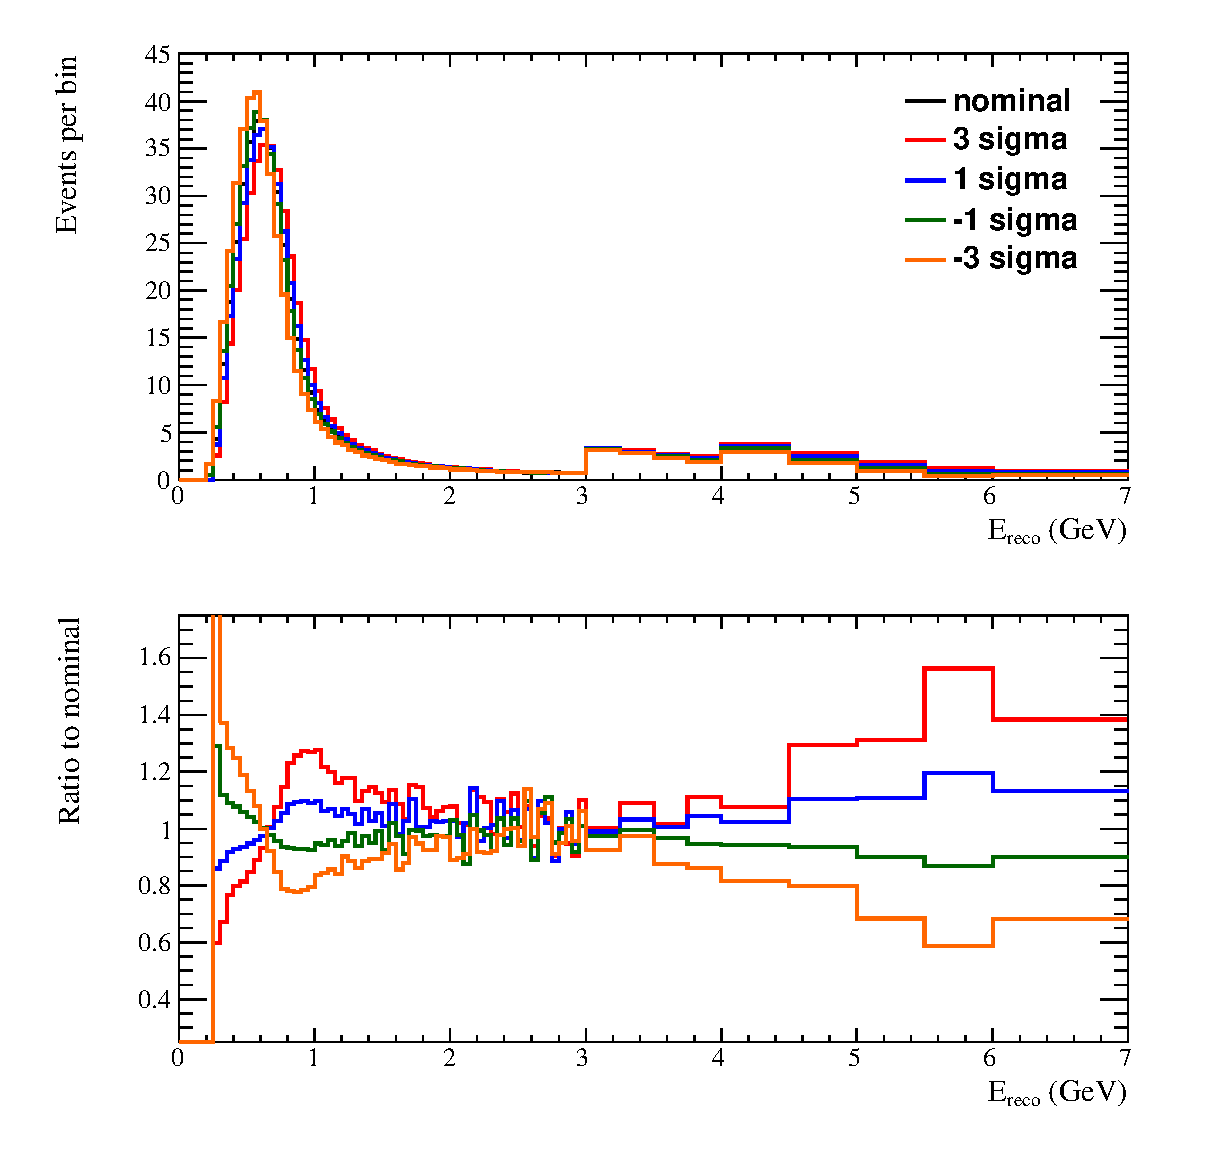
\includegraphics{../images/spectrum_tweaked/1sigma_unoscillated/ereco_twk_f_sk_e_scale}}
\caption
{ Effect of $f_{E; r}^{SK}$   for no oscillations (all mixing angles set to 0). }
\label{fig:noosc_ereco_twk_f_sk_e_scale}
\end{center}
\end{figure}
\clearpage

\begin{figure}
\begin{center}
\resizebox{14cm}{!}{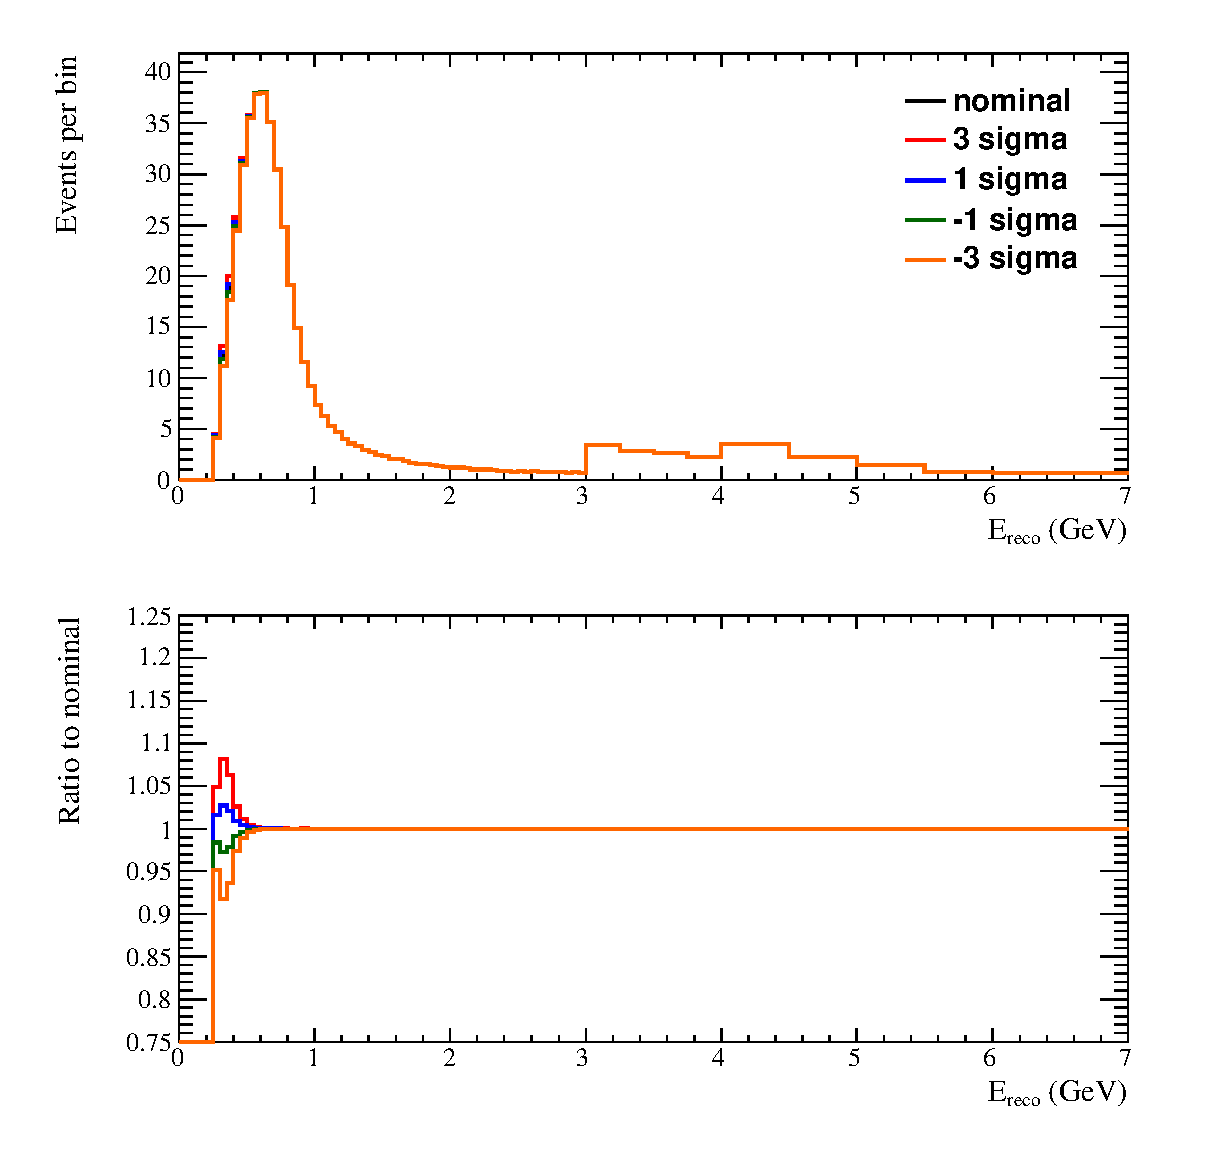
\includegraphics{../images/spectrum_tweaked/1sigma_unoscillated/ereco_twk_f_banff00}}
\caption
{ Effect of $f_{0; t, r}^{banff}$ for no oscillations (all mixing angles set to 0). }
\label{fig:noosc_ereco_twk_f_banff00}
\end{center}
\end{figure}
\clearpage

\begin{figure}
\begin{center}
\resizebox{14cm}{!}{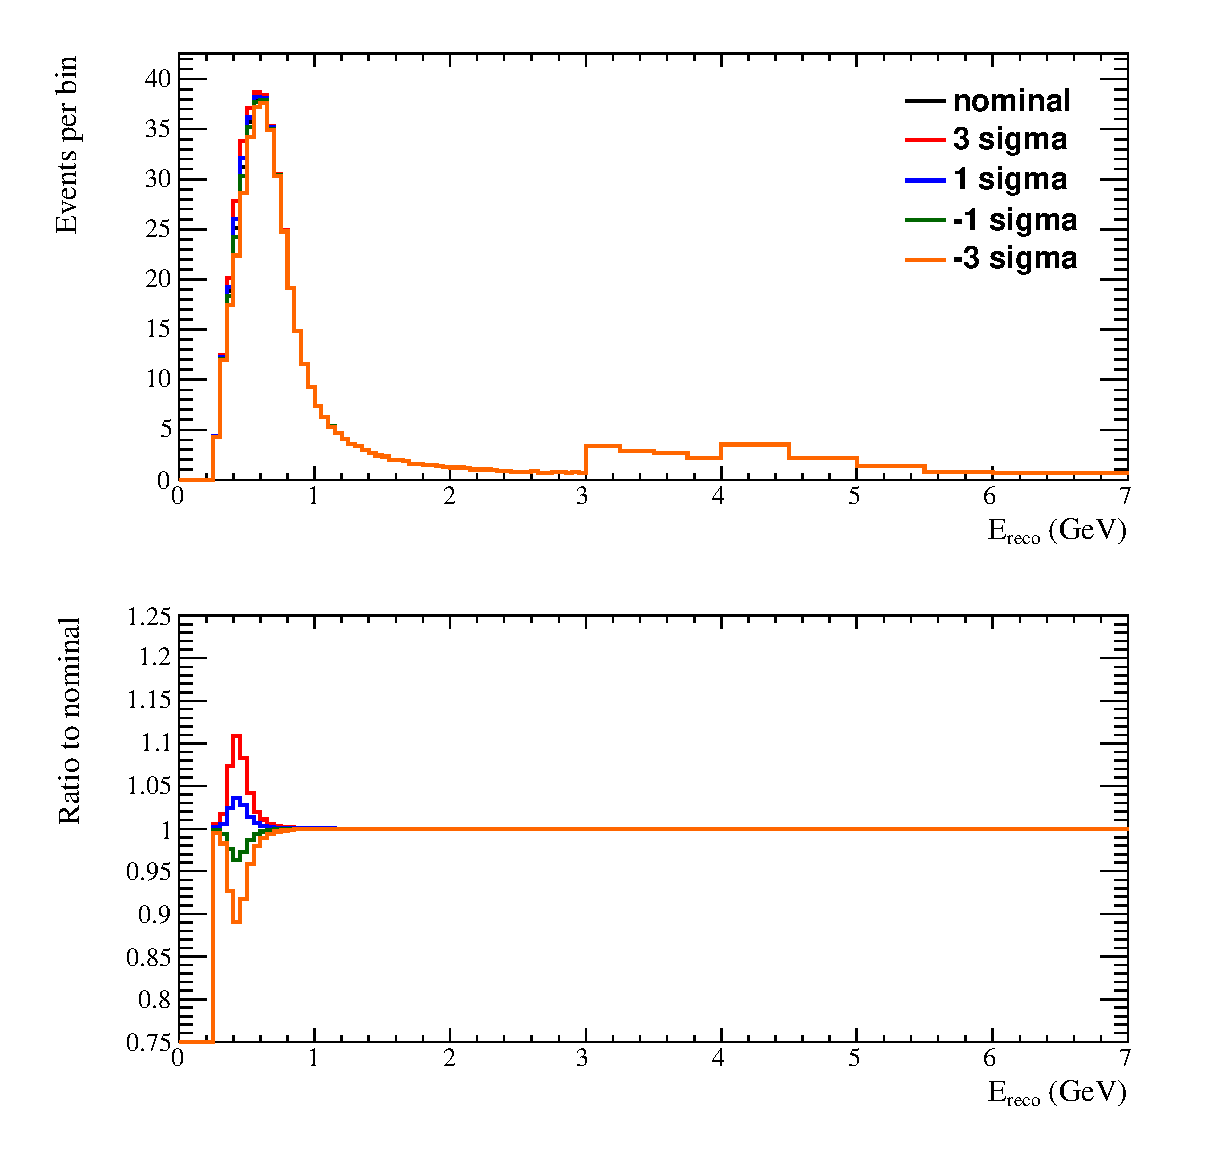
\includegraphics{../images/spectrum_tweaked/1sigma_unoscillated/ereco_twk_f_banff01}}
\caption
{ Effect of $f_{1; t, r}^{banff}$ for no oscillations (all mixing angles set to 0). }
\label{fig:noosc_ereco_twk_f_banff01}
\end{center}
\end{figure}
\clearpage

\begin{figure}
\begin{center}
\resizebox{14cm}{!}{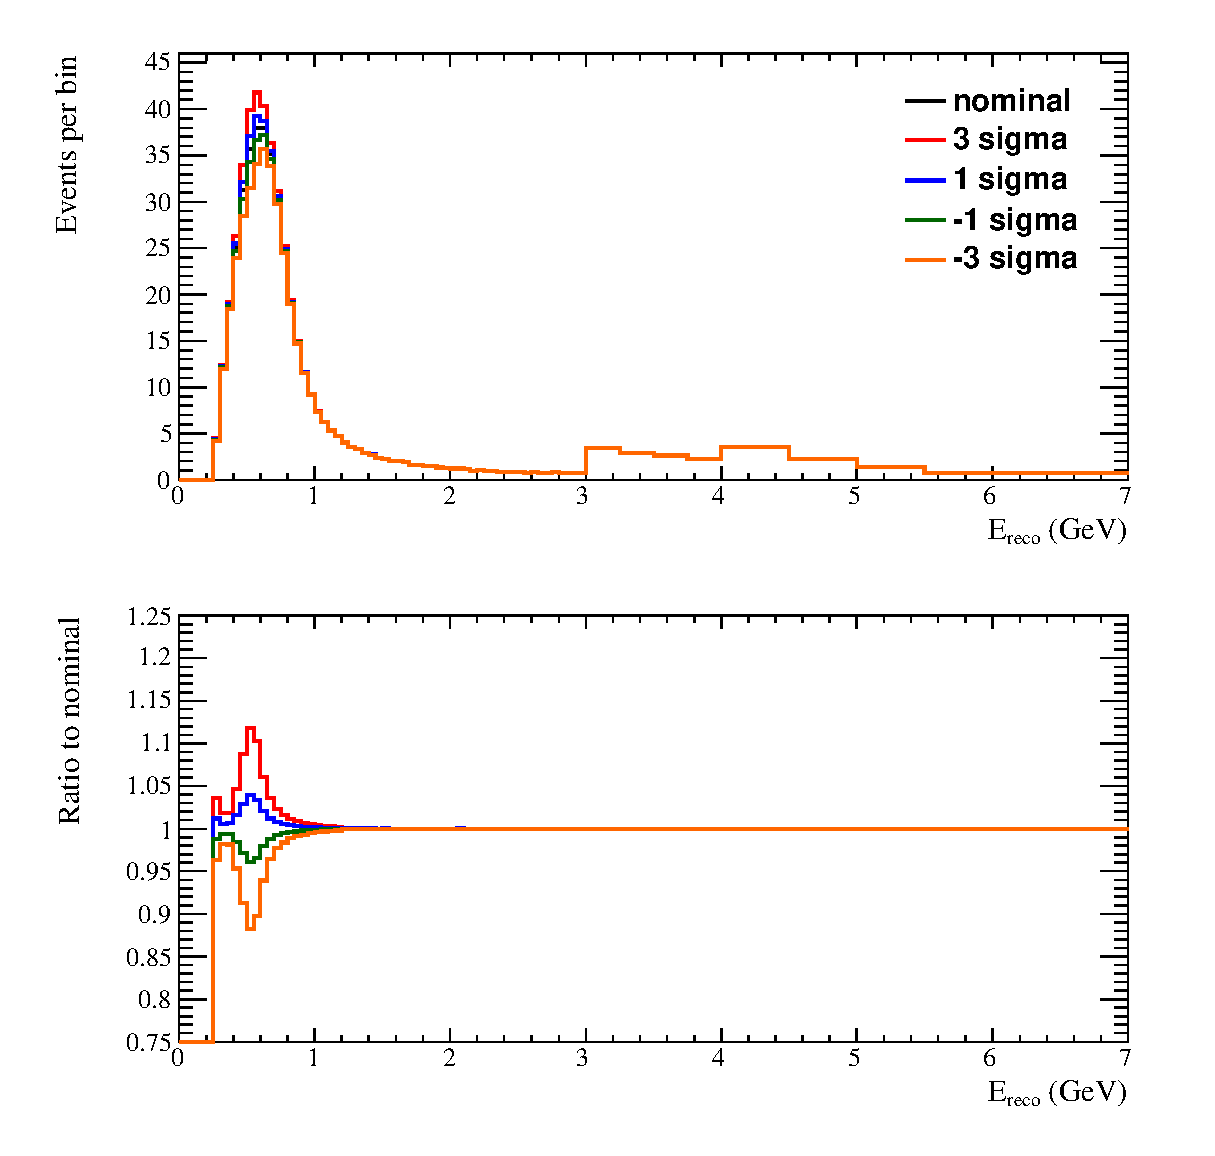
\includegraphics{../images/spectrum_tweaked/1sigma_unoscillated/ereco_twk_f_banff02}}
\caption
{ Effect of $f_{2; t, r}^{banff}$ for no oscillations (all mixing angles set to 0). }
\label{fig:noosc_ereco_twk_f_banff02}
\end{center}
\end{figure}
\clearpage

\begin{figure}
\begin{center}
\resizebox{14cm}{!}{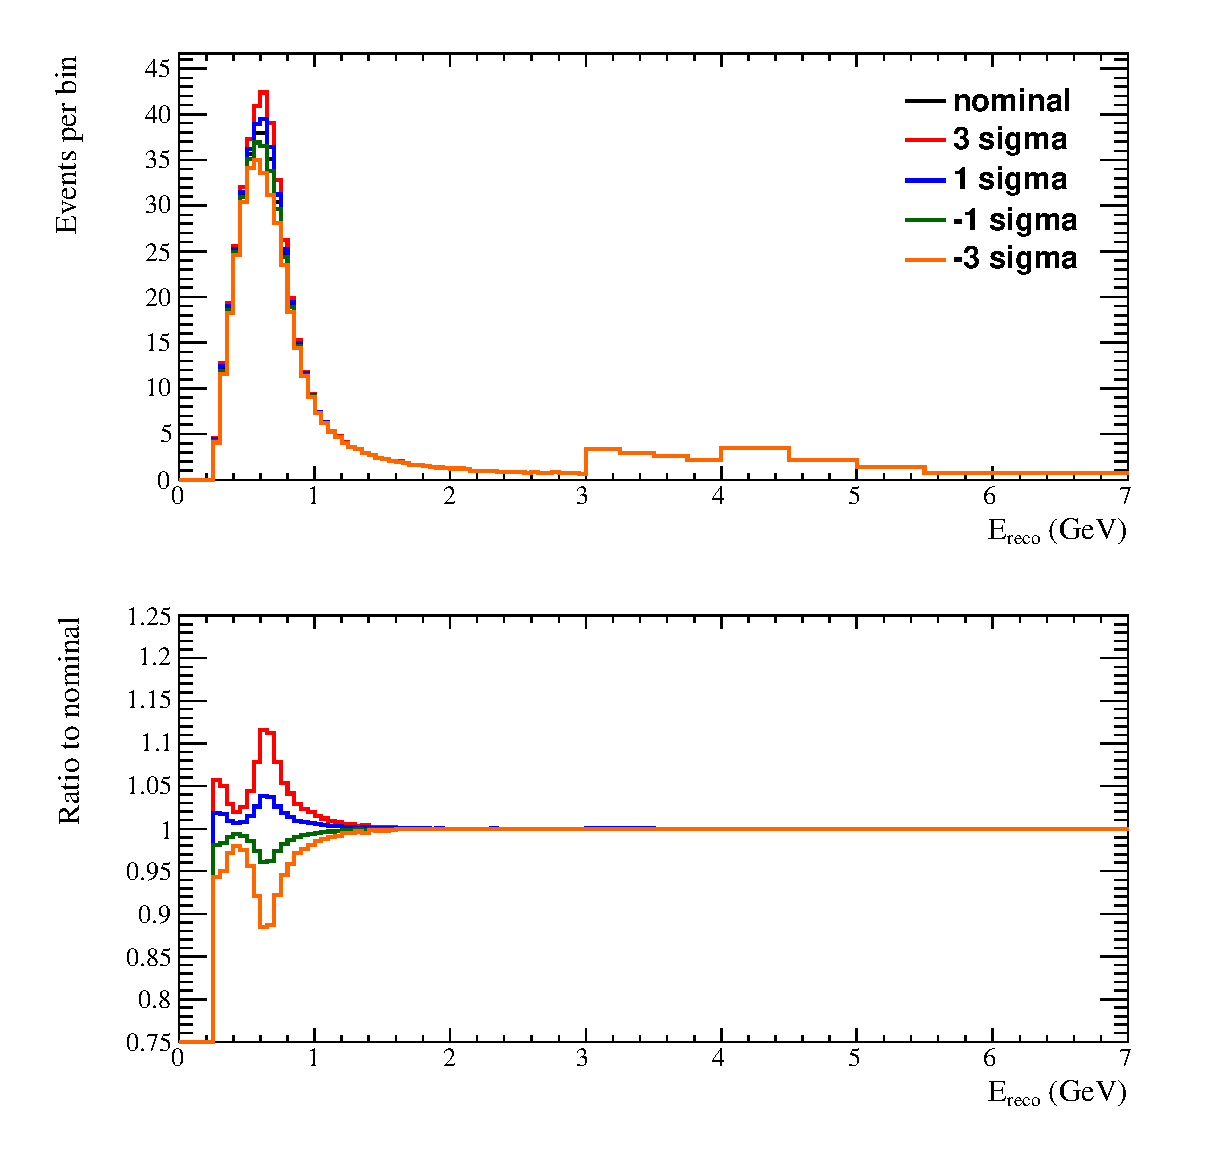
\includegraphics{../images/spectrum_tweaked/1sigma_unoscillated/ereco_twk_f_banff03}}
\caption
{ Effect of $f_{3; t, r}^{banff}$ for no oscillations (all mixing angles set to 0). }
\label{fig:noosc_ereco_twk_f_banff03}
\end{center}
\end{figure}
\clearpage

\begin{figure}
\begin{center}
\resizebox{14cm}{!}{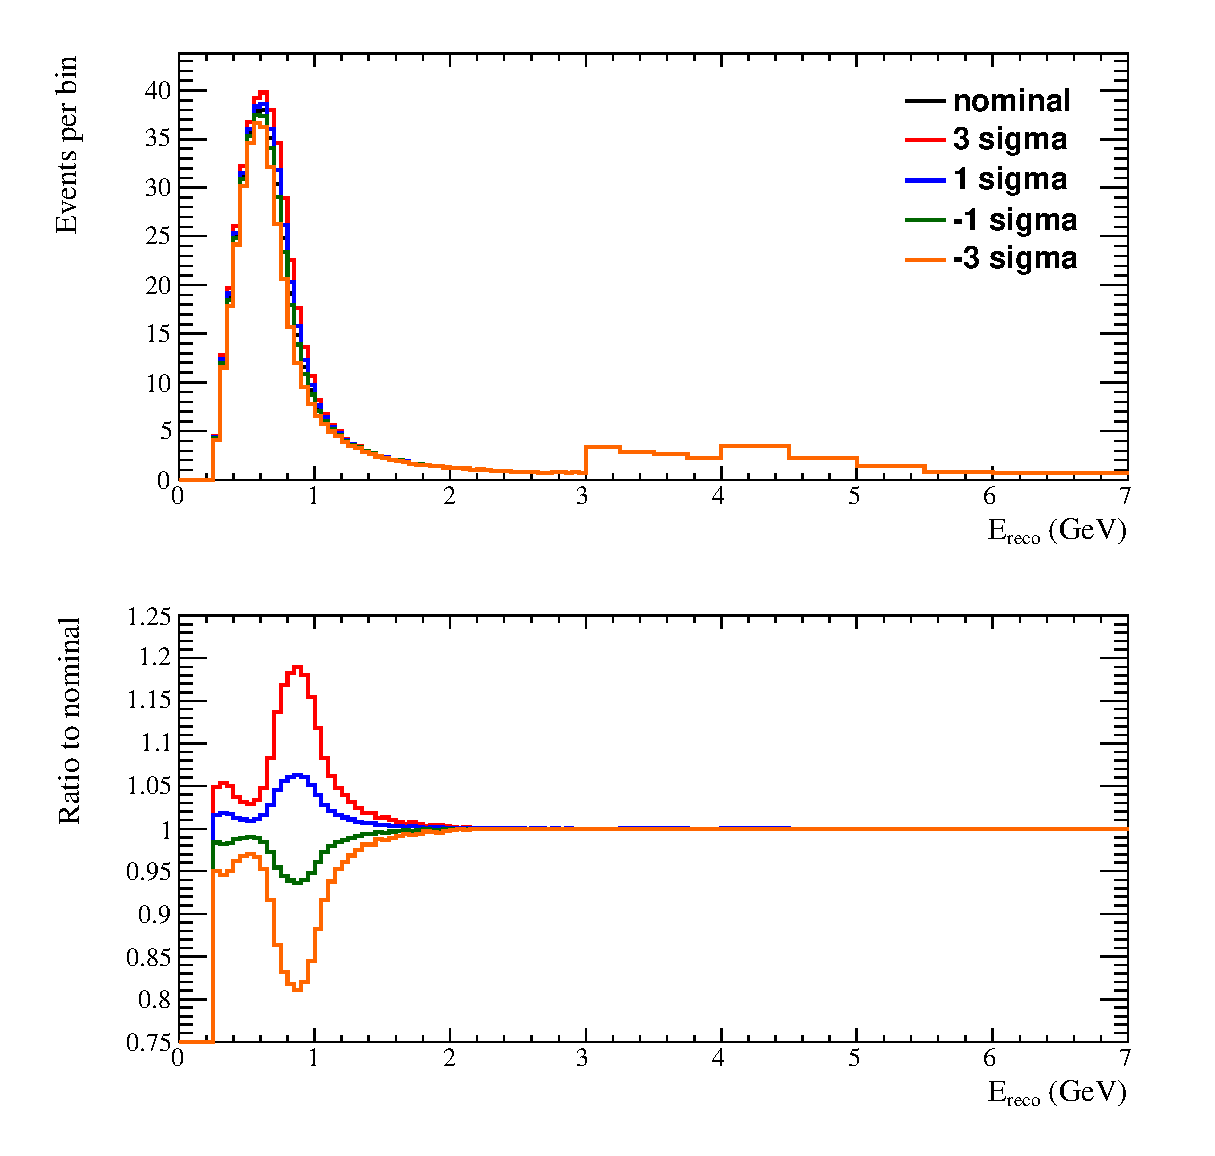
\includegraphics{../images/spectrum_tweaked/1sigma_unoscillated/ereco_twk_f_banff04}}
\caption
{ Effect of $f_{4; t, r}^{banff}$ for no oscillations (all mixing angles set to 0). }
\label{fig:noosc_ereco_twk_f_banff04}
\end{center}
\end{figure}
\clearpage

\begin{figure}
\begin{center}
\resizebox{14cm}{!}{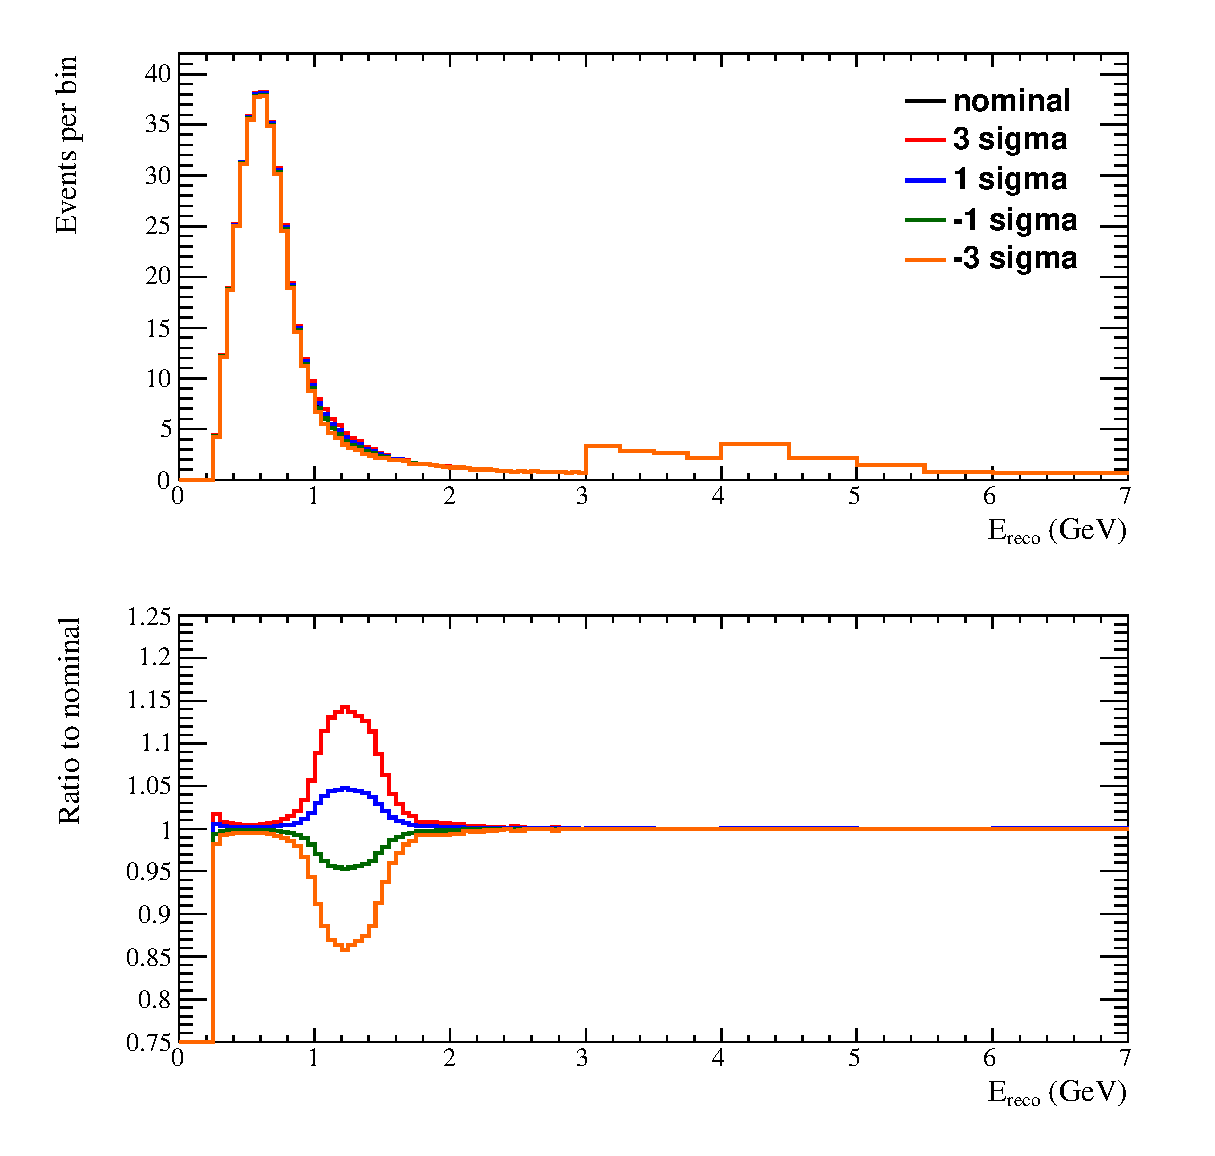
\includegraphics{../images/spectrum_tweaked/1sigma_unoscillated/ereco_twk_f_banff05}}
\caption
{ Effect of $f_{5; t, r}^{banff}$ for no oscillations (all mixing angles set to 0). }
\label{fig:noosc_ereco_twk_f_banff05}
\end{center}
\end{figure}
\clearpage

\begin{figure}
\begin{center}
\resizebox{14cm}{!}{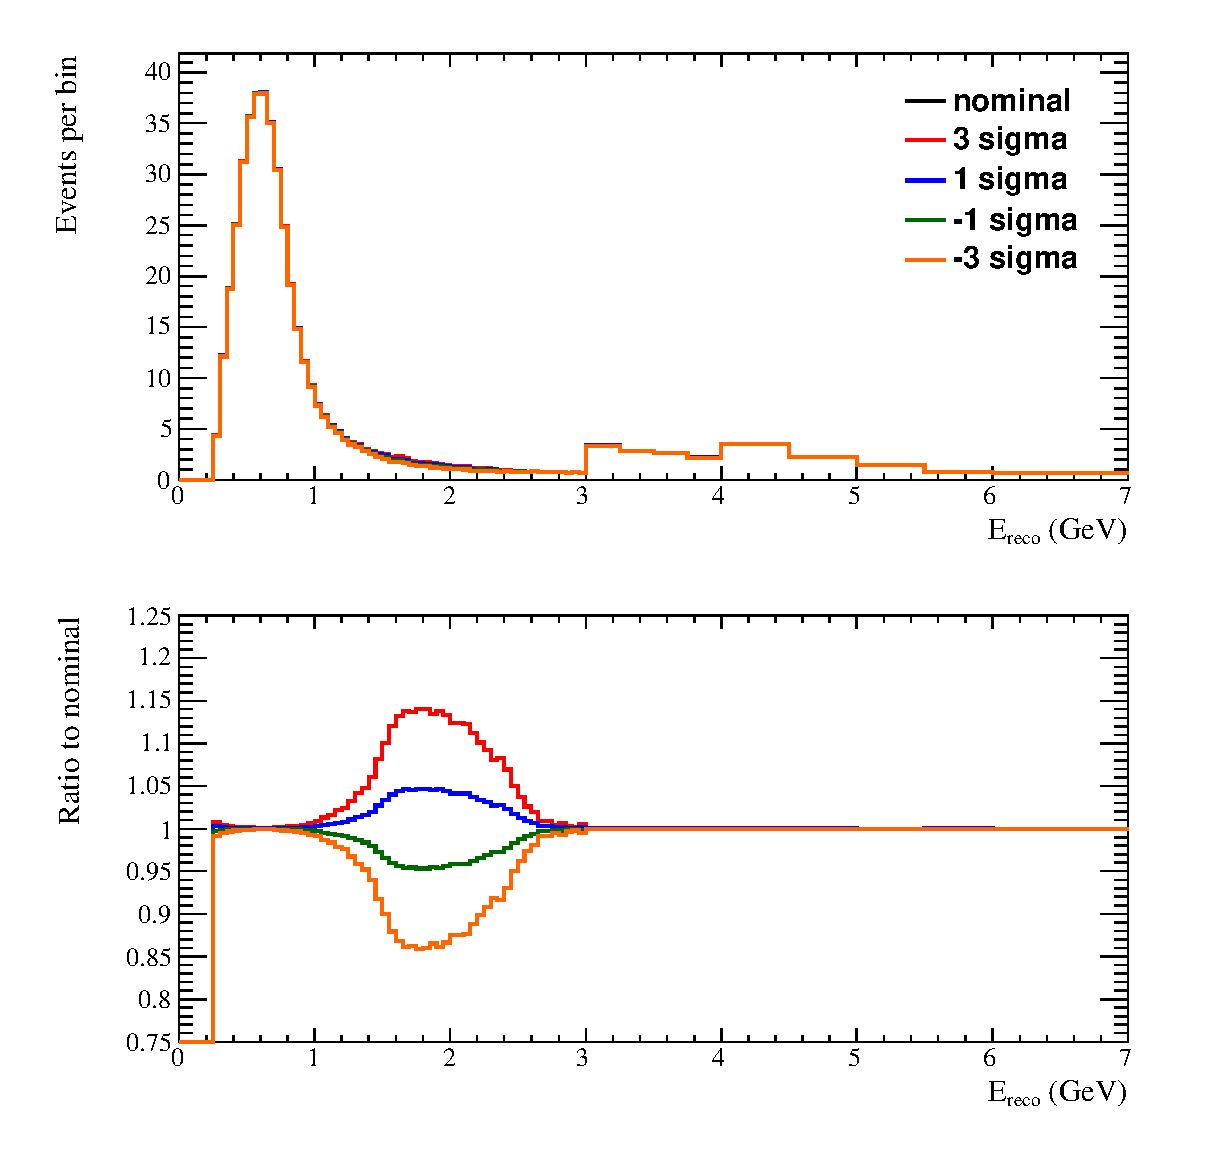
\includegraphics{../images/spectrum_tweaked/1sigma_unoscillated/ereco_twk_f_banff06}}
\caption
{ Effect of $f_{6; t, r}^{banff}$ for no oscillations (all mixing angles set to 0). }
\label{fig:noosc_ereco_twk_f_banff06}
\end{center}
\end{figure}
\clearpage

\begin{figure}
\begin{center}
\resizebox{14cm}{!}{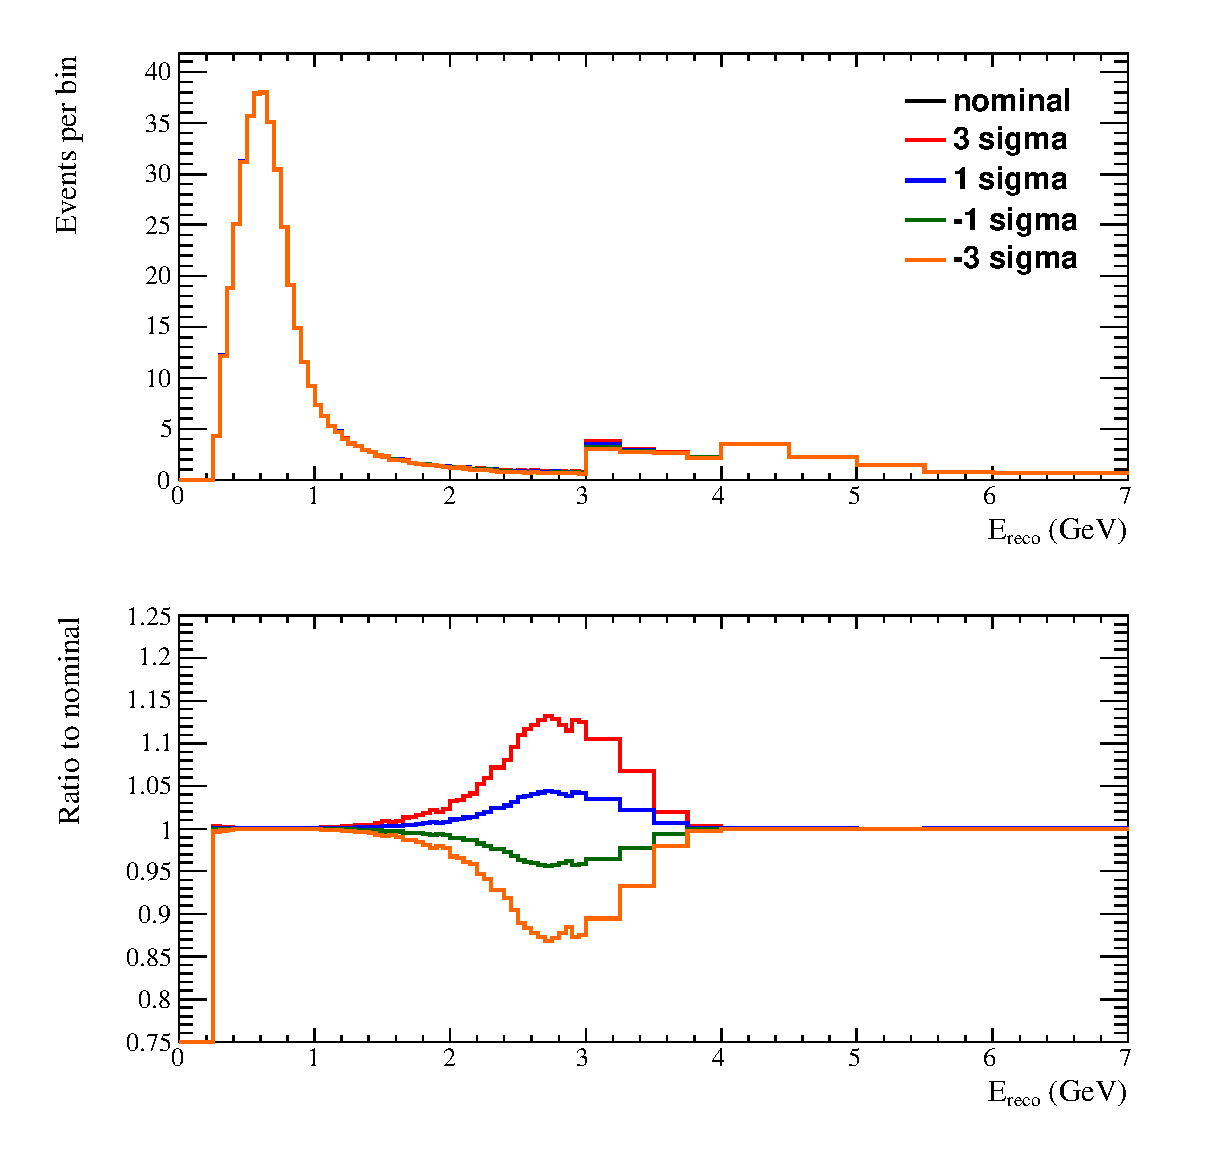
\includegraphics{../images/spectrum_tweaked/1sigma_unoscillated/ereco_twk_f_banff07}}
\caption
{ Effect of $f_{7; t, r}^{banff}$ for no oscillations (all mixing angles set to 0). }
\label{fig:noosc_ereco_twk_f_banff07}
\end{center}
\end{figure}
\clearpage

\begin{figure}
\begin{center}
\resizebox{14cm}{!}{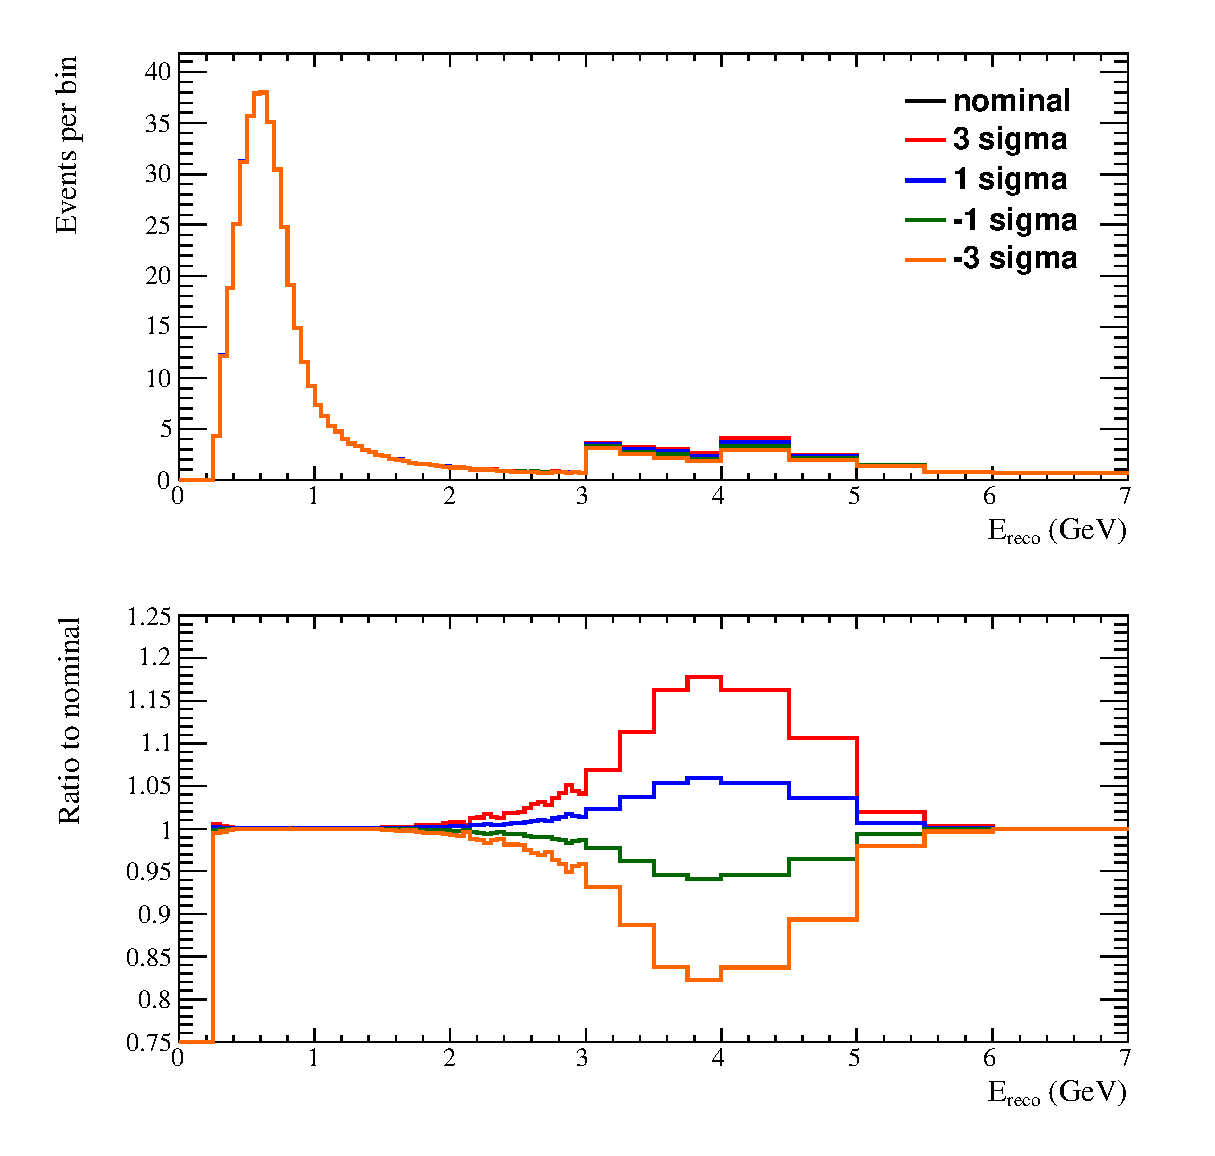
\includegraphics{../images/spectrum_tweaked/1sigma_unoscillated/ereco_twk_f_banff08}}
\caption
{ Effect of $f_{8; t, r}^{banff}$ for no oscillations (all mixing angles set to 0). }
\label{fig:noosc_ereco_twk_f_banff08}
\end{center}
\end{figure}
\clearpage

\begin{figure}
\begin{center}
\resizebox{14cm}{!}{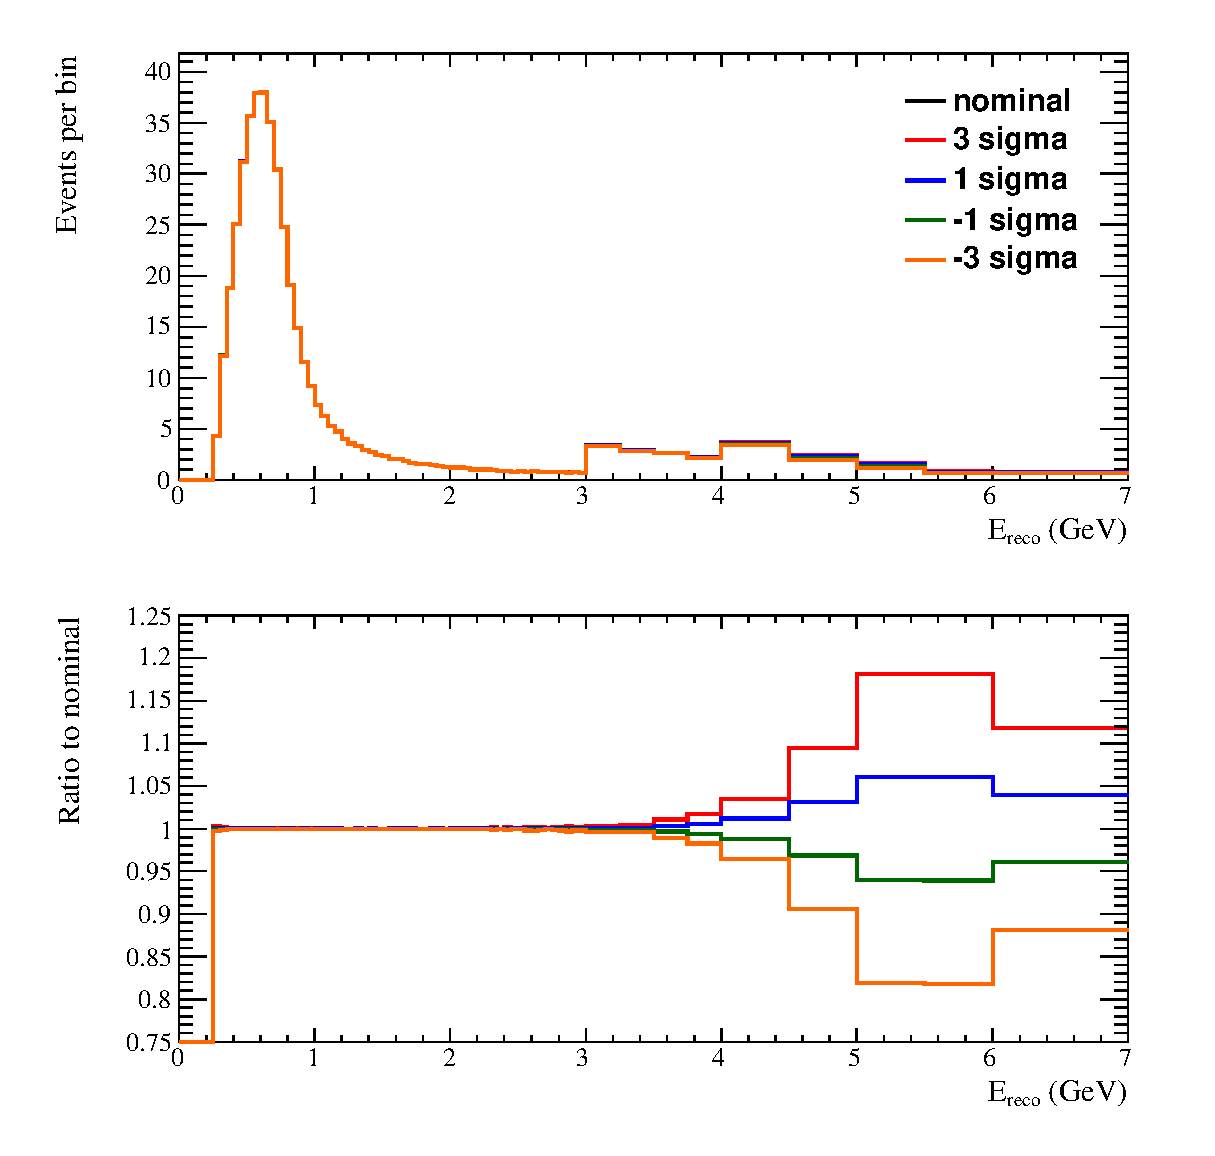
\includegraphics{../images/spectrum_tweaked/1sigma_unoscillated/ereco_twk_f_banff09}}
\caption
{ Effect of $f_{9; t, r}^{banff}$ for no oscillations (all mixing angles set to 0). }
\label{fig:noosc_ereco_twk_f_banff09}
\end{center}
\end{figure}
\clearpage

\begin{figure}
\begin{center}
\resizebox{14cm}{!}{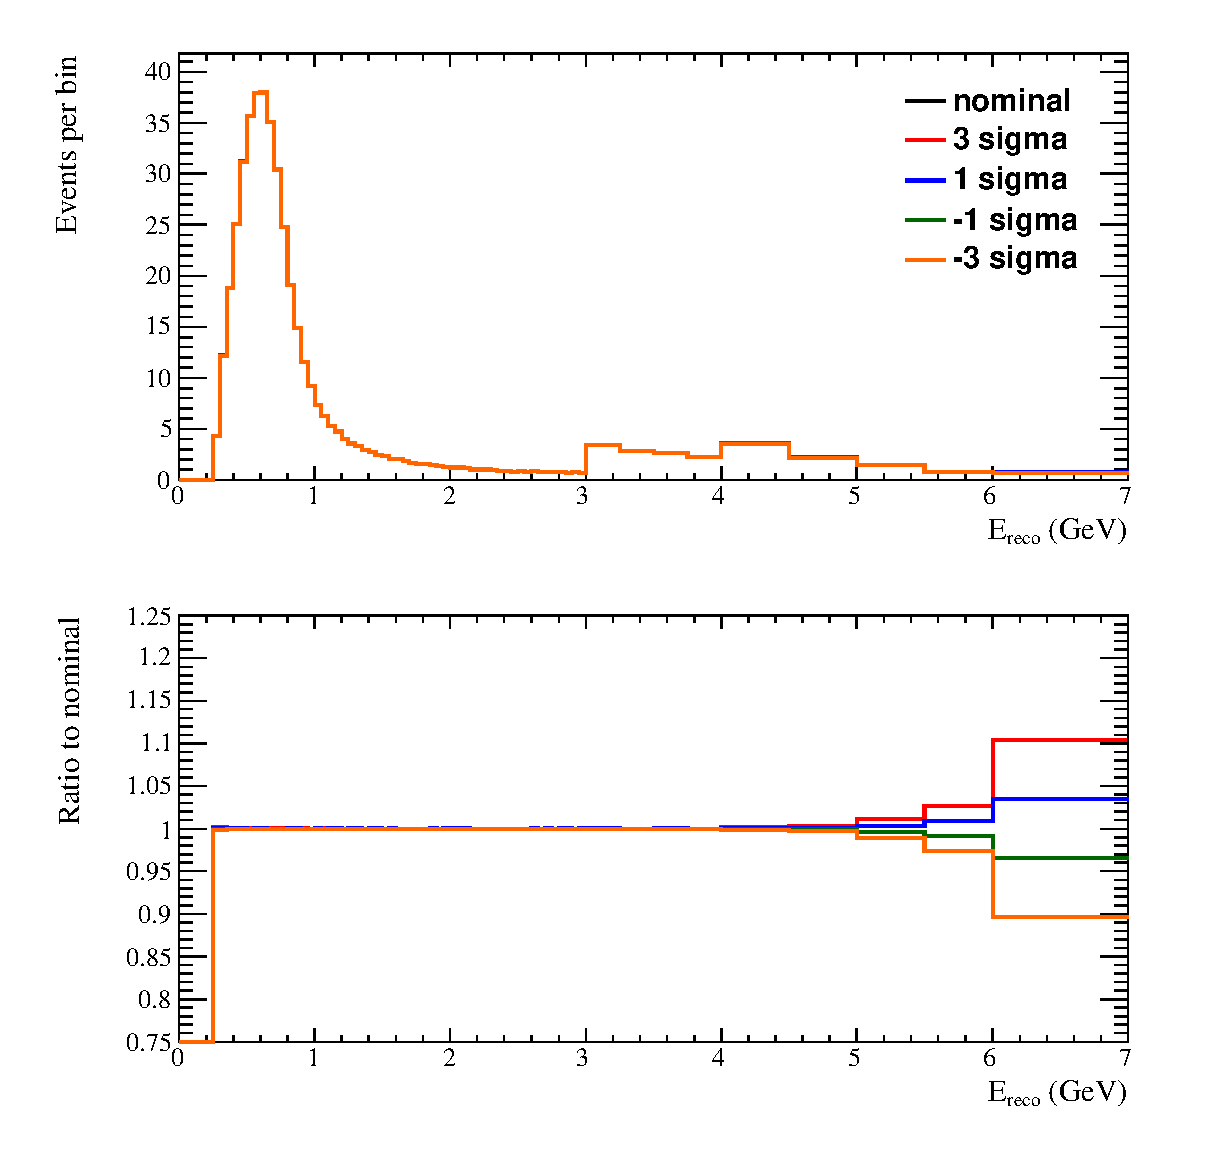
\includegraphics{../images/spectrum_tweaked/1sigma_unoscillated/ereco_twk_f_banff10}}
\caption
{ Effect of $f_{10; t, r}^{banff}$ for no oscillations (all mixing angles set to 0). }
\label{fig:noosc_ereco_twk_f_banff10}
\end{center}
\end{figure}
\clearpage

\begin{figure}
\begin{center}
\resizebox{14cm}{!}{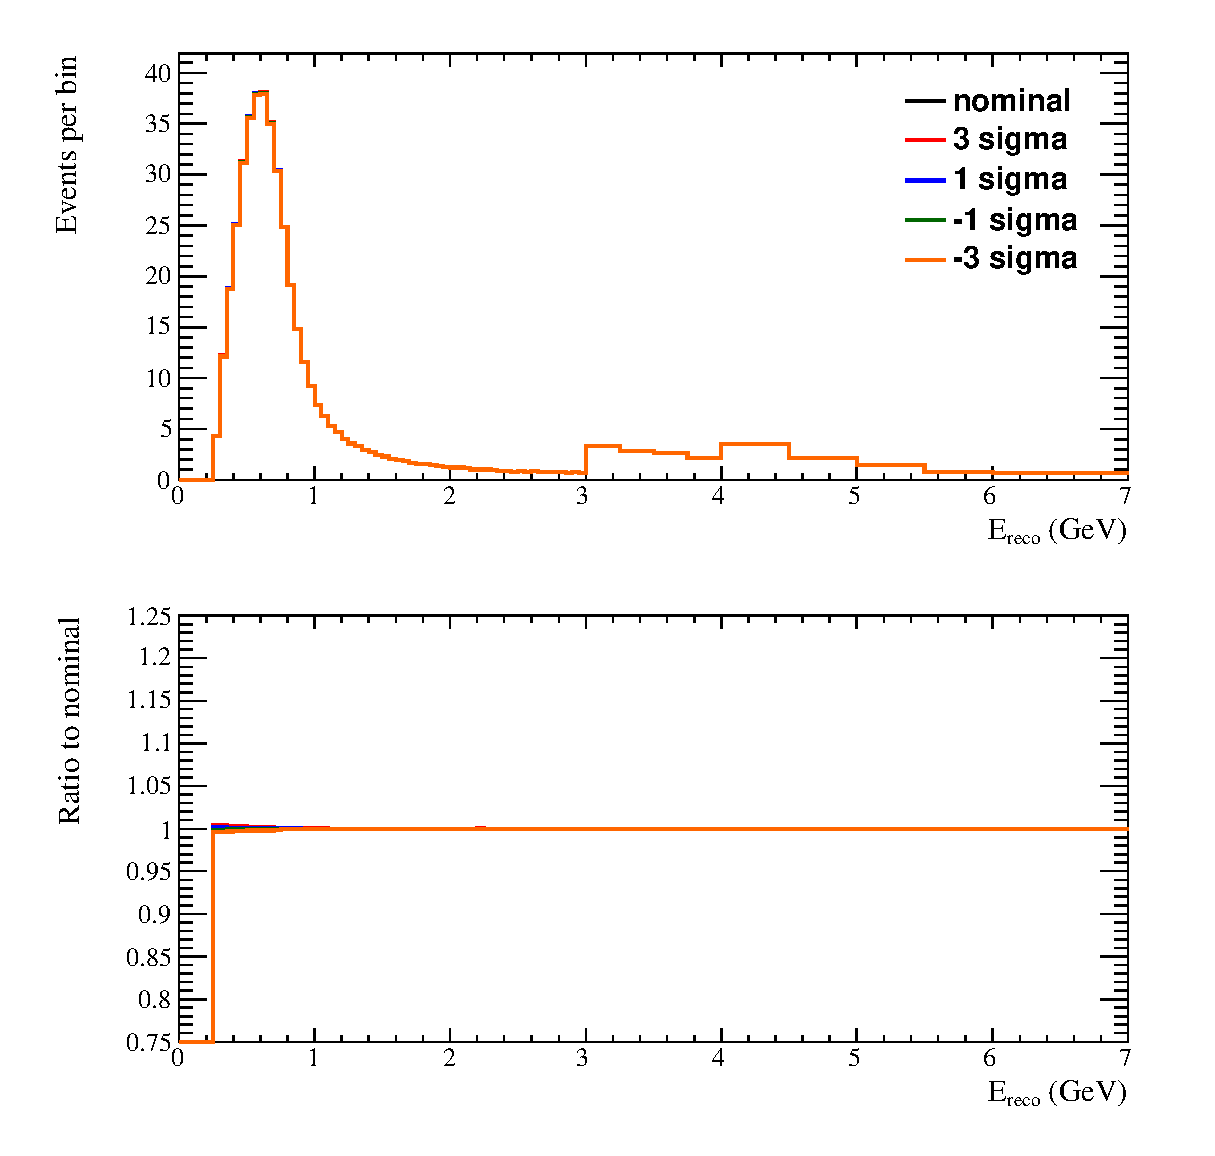
\includegraphics{../images/spectrum_tweaked/1sigma_unoscillated/ereco_twk_f_banff11}}
\caption
{ Effect of $f_{11; t, r}^{banff}$ for no oscillations (all mixing angles set to 0). }
\label{fig:noosc_ereco_twk_f_banff11}
\end{center}
\end{figure}
\clearpage

\begin{figure}
\begin{center}
\resizebox{14cm}{!}{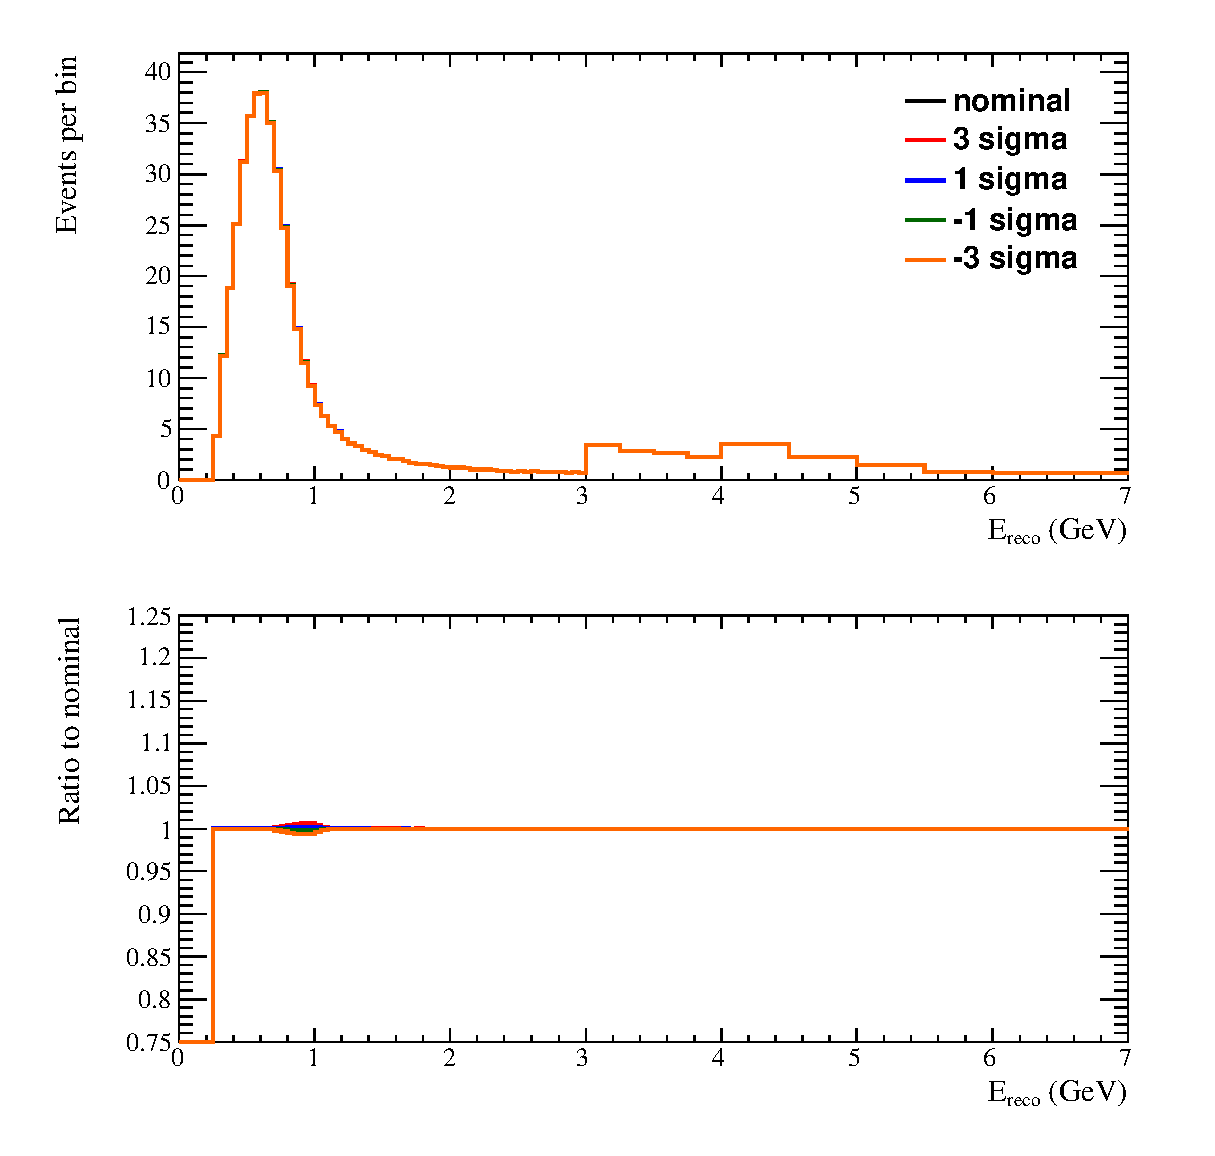
\includegraphics{../images/spectrum_tweaked/1sigma_unoscillated/ereco_twk_f_banff12}}
\caption
{ Effect of $f_{12; t, r}^{banff}$ for no oscillations (all mixing angles set to 0). }
\label{fig:noosc_ereco_twk_f_banff12}
\end{center}
\end{figure}
\clearpage

\begin{figure}
\begin{center}
\resizebox{14cm}{!}{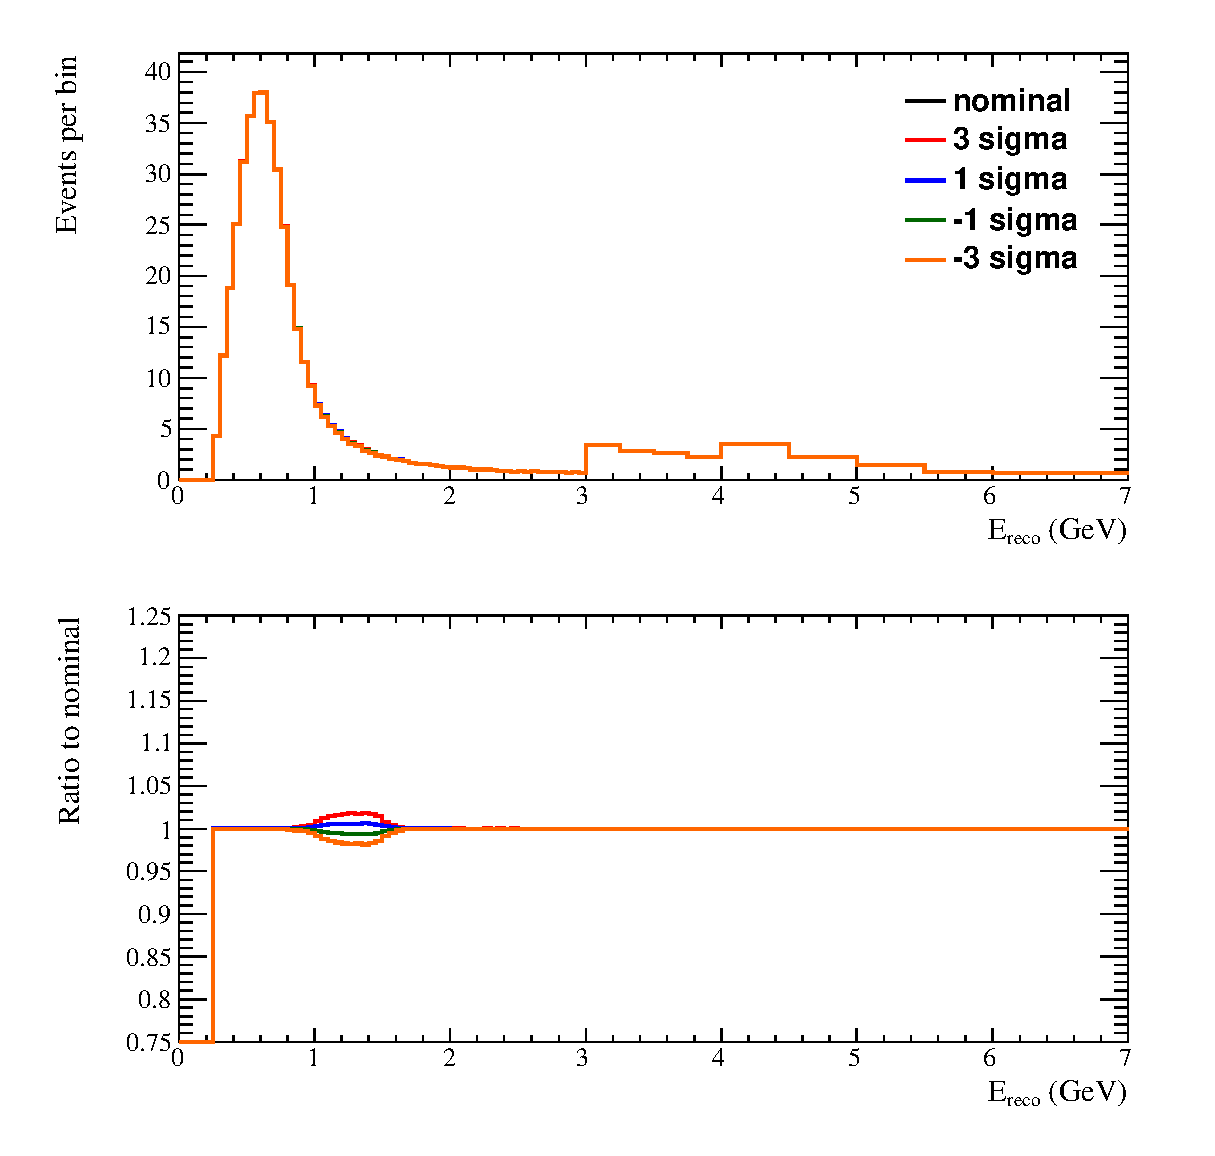
\includegraphics{../images/spectrum_tweaked/1sigma_unoscillated/ereco_twk_f_banff13}}
\caption
{ Effect of $f_{13; t, r}^{banff}$ for no oscillations (all mixing angles set to 0). }
\label{fig:noosc_ereco_twk_f_banff13}
\end{center}
\end{figure}
\clearpage

\begin{figure}
\begin{center}
\resizebox{14cm}{!}{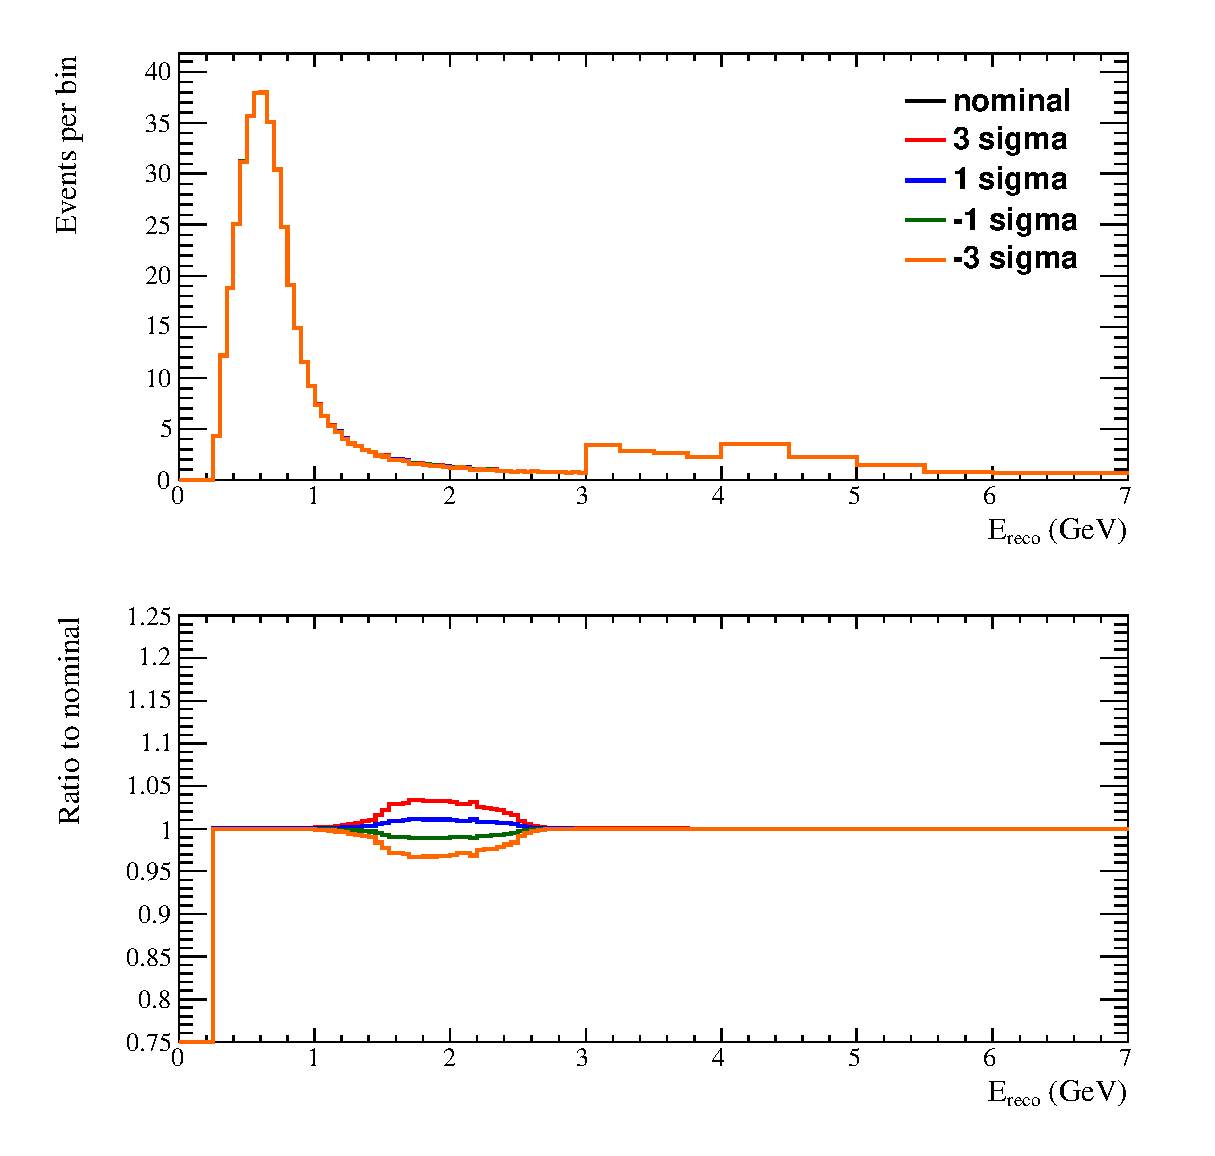
\includegraphics{../images/spectrum_tweaked/1sigma_unoscillated/ereco_twk_f_banff14}}
\caption
{ Effect of $f_{14; t, r}^{banff}$ for no oscillations (all mixing angles set to 0). }
\label{fig:noosc_ereco_twk_f_banff14}
\end{center}
\end{figure}
\clearpage

\begin{figure}
\begin{center}
\resizebox{14cm}{!}{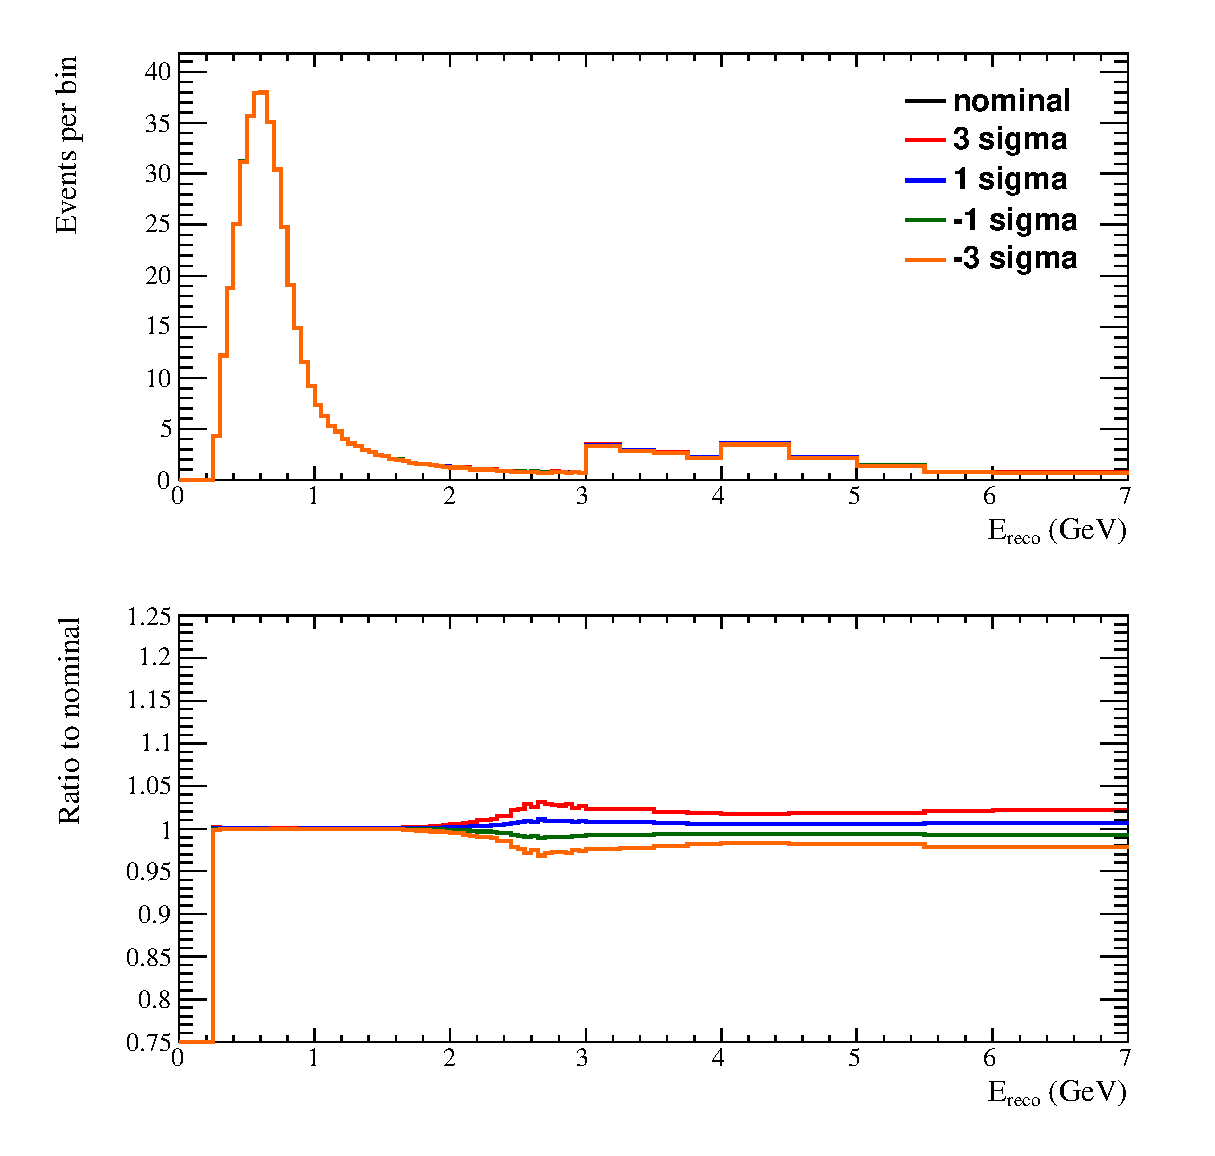
\includegraphics{../images/spectrum_tweaked/1sigma_unoscillated/ereco_twk_f_banff15}}
\caption
{ Effect of $f_{15; t, r}^{banff}$ for no oscillations (all mixing angles set to 0). }
\label{fig:noosc_ereco_twk_f_banff15}
\end{center}
\end{figure}
\clearpage

\begin{figure}
\begin{center}
\resizebox{14cm}{!}{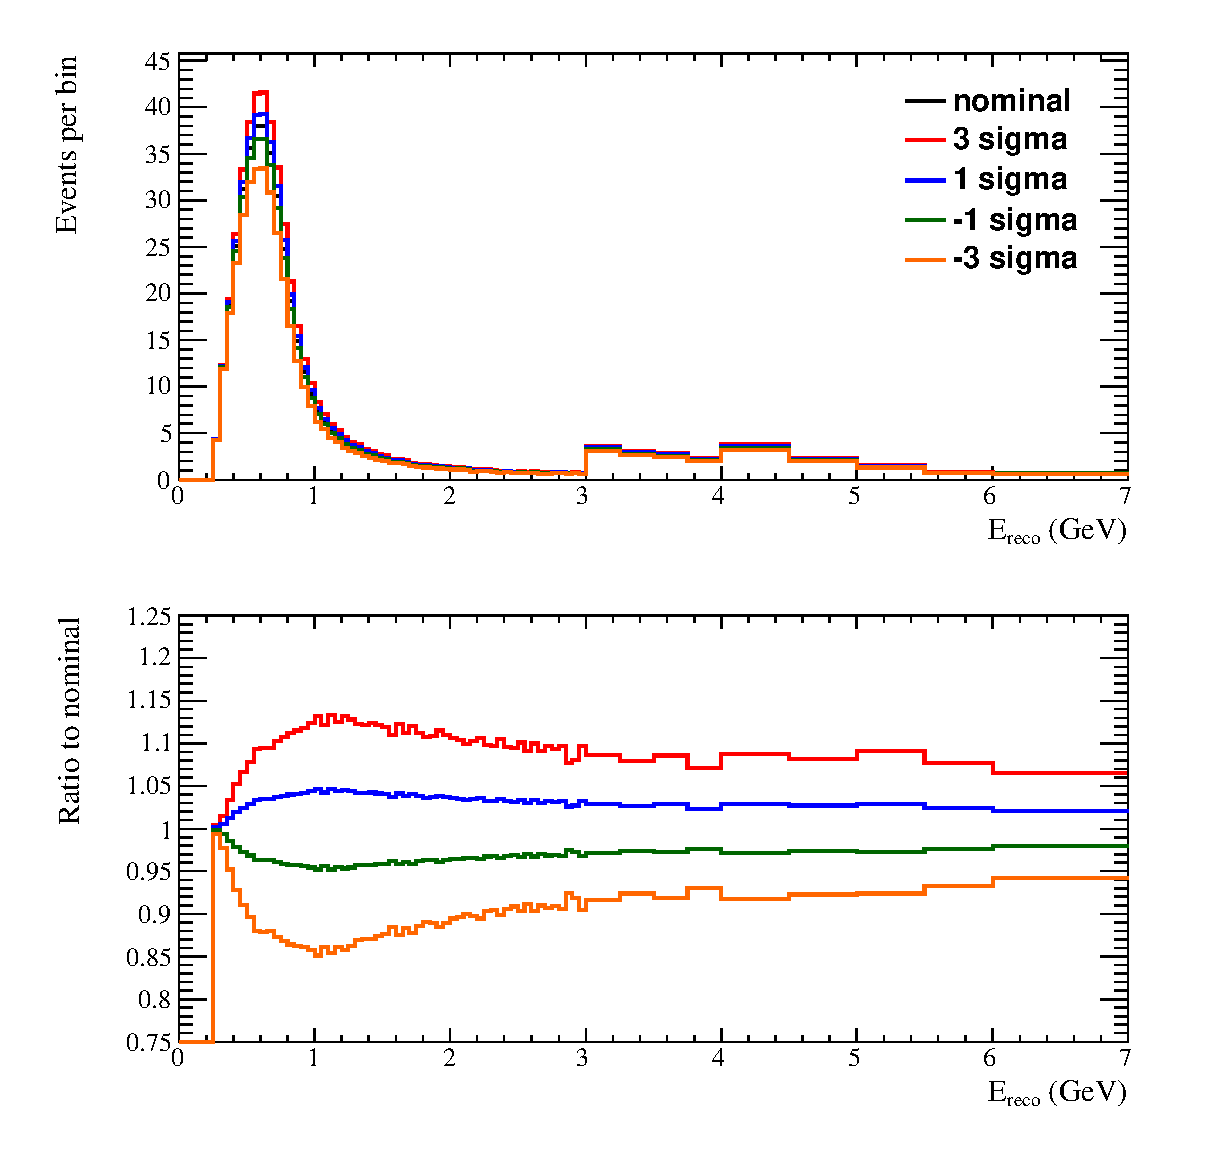
\includegraphics{../images/spectrum_tweaked/1sigma_unoscillated/ereco_twk_f_banffmaqe}}
\caption
{ Effect of $f_{16; t, r}^{banff}$ for no oscillations (all mixing angles set to 0). }
\label{fig:noosc_ereco_twk_f_banffmaqe}
\end{center}
\end{figure}
\clearpage

\begin{figure}
\begin{center}
\resizebox{14cm}{!}{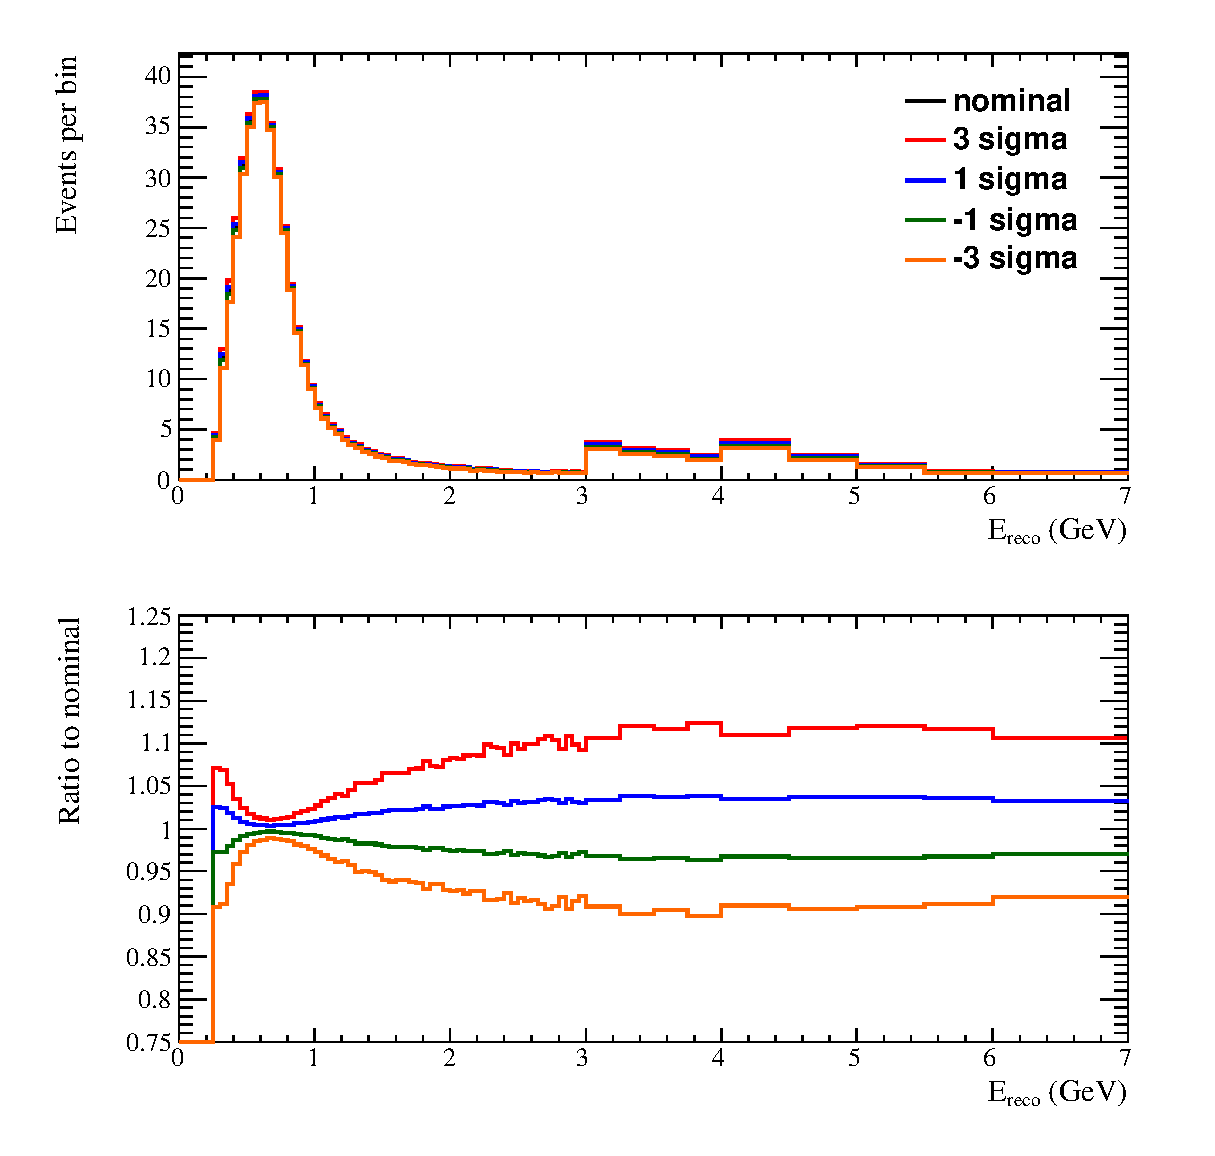
\includegraphics{../images/spectrum_tweaked/1sigma_unoscillated/ereco_twk_f_banffmares}}
\caption
{ Effect of $f_{17; t, r}^{banff}$ for no oscillations (all mixing angles set to 0). }
\label{fig:noosc_ereco_twk_f_banffmares}
\end{center}
\end{figure}
\clearpage

\begin{figure}
\begin{center}
\resizebox{14cm}{!}{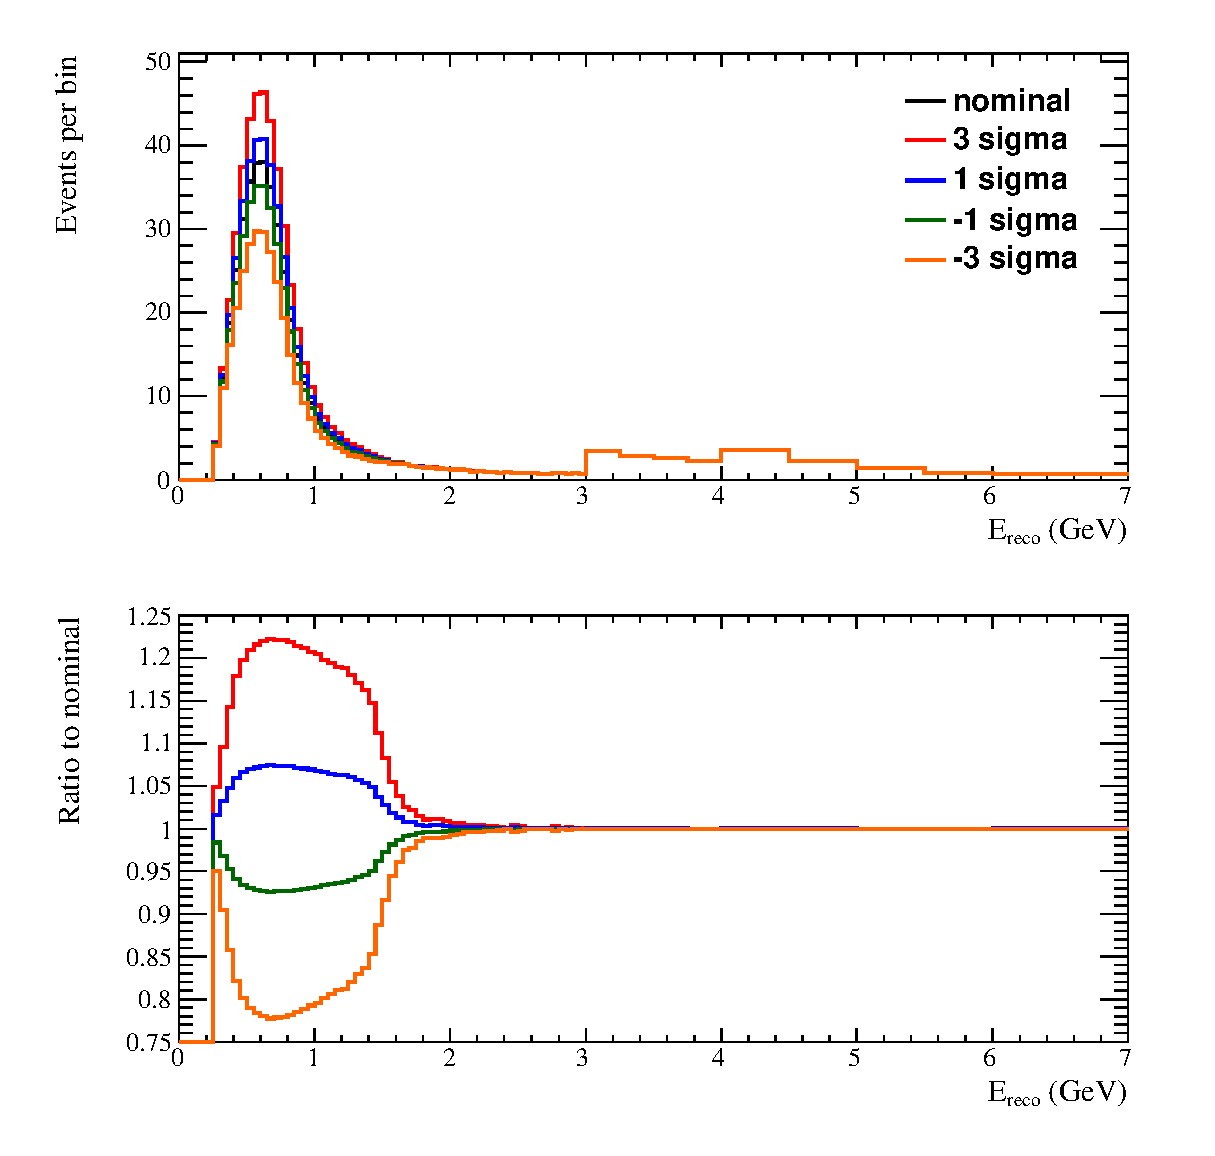
\includegraphics{../images/spectrum_tweaked/1sigma_unoscillated/ereco_twk_f_banffccqee0}}
\caption
{ Effect of $f_{18; t, r}^{banff}$ for no oscillations (all mixing angles set to 0). }
\label{fig:noosc_ereco_twk_f_banffccqee0}
\end{center}
\end{figure}
\clearpage

\begin{figure}
\begin{center}
\resizebox{14cm}{!}{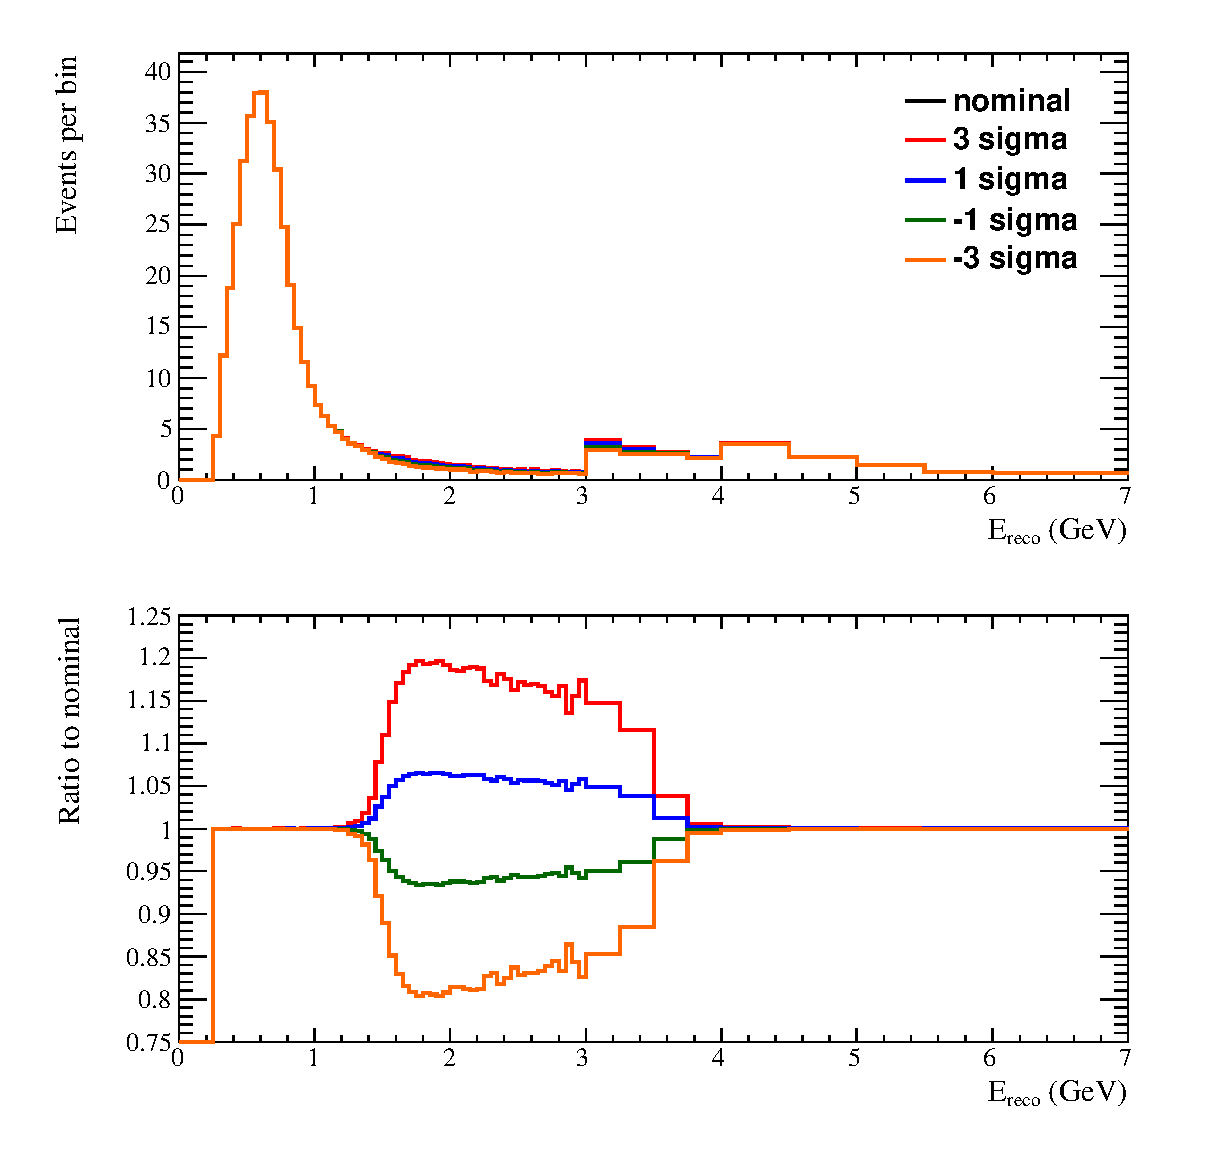
\includegraphics{../images/spectrum_tweaked/1sigma_unoscillated/ereco_twk_f_banffccqee1}}
\caption
{ Effect of $f_{19; t, r}^{banff}$ for no oscillations (all mixing angles set to 0). }
\label{fig:noosc_ereco_twk_f_banffccqee1}
\end{center}
\end{figure}
\clearpage

\begin{figure}
\begin{center}
\resizebox{14cm}{!}{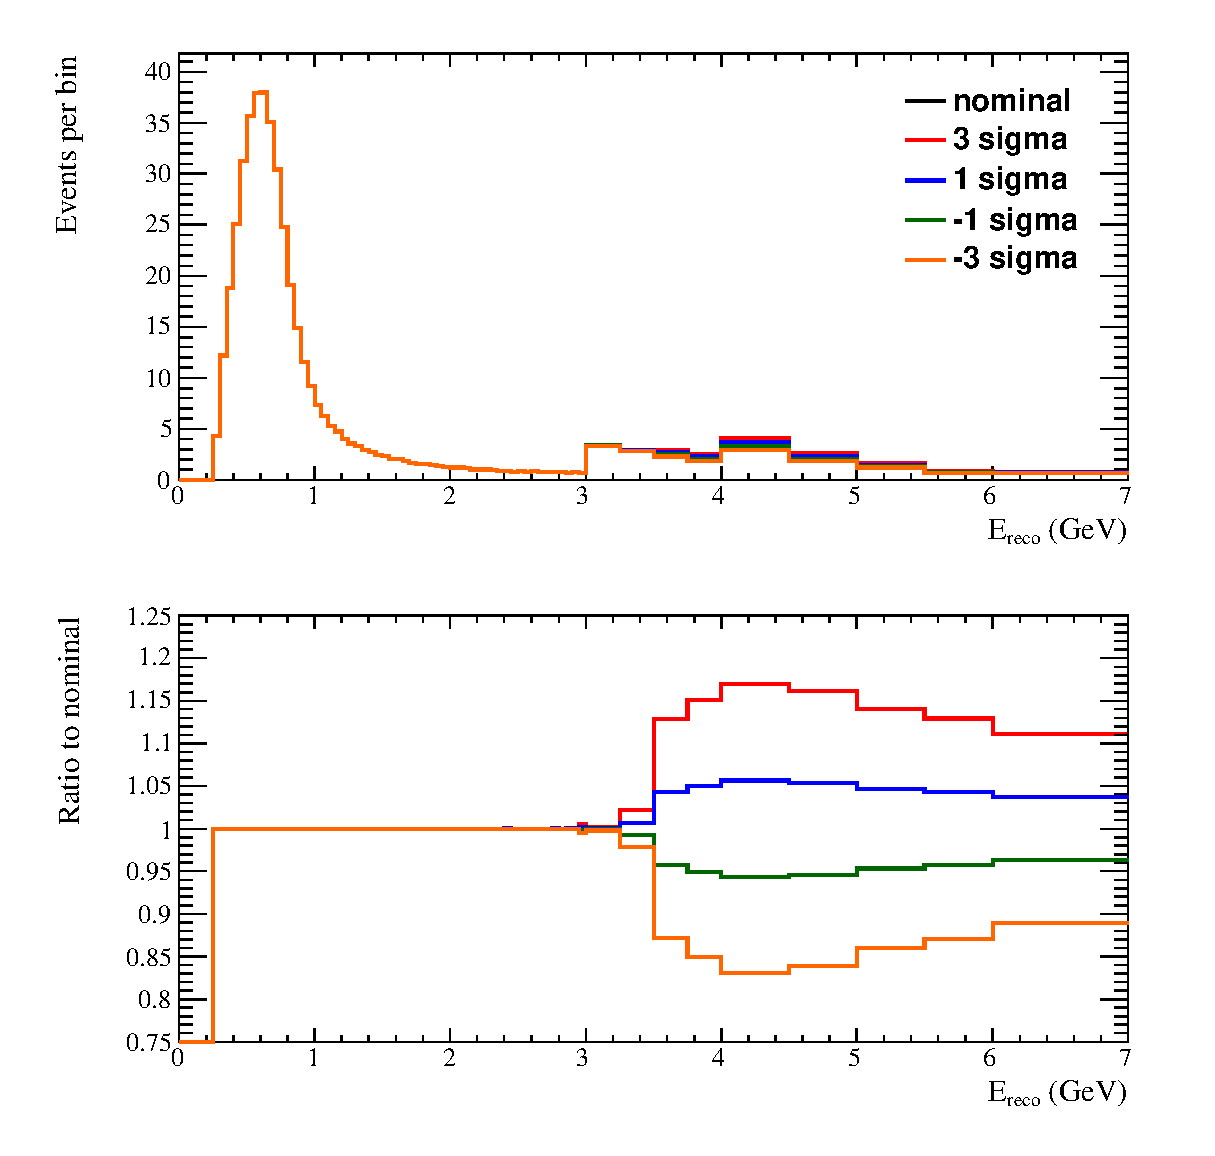
\includegraphics{../images/spectrum_tweaked/1sigma_unoscillated/ereco_twk_f_banffccqee2}}
\caption
{ Effect of $f_{20; t, r}^{banff}$ for no oscillations (all mixing angles set to 0). }
\label{fig:noosc_ereco_twk_f_banffccqee2}
\end{center}
\end{figure}
\clearpage

\begin{figure}
\begin{center}
\resizebox{14cm}{!}{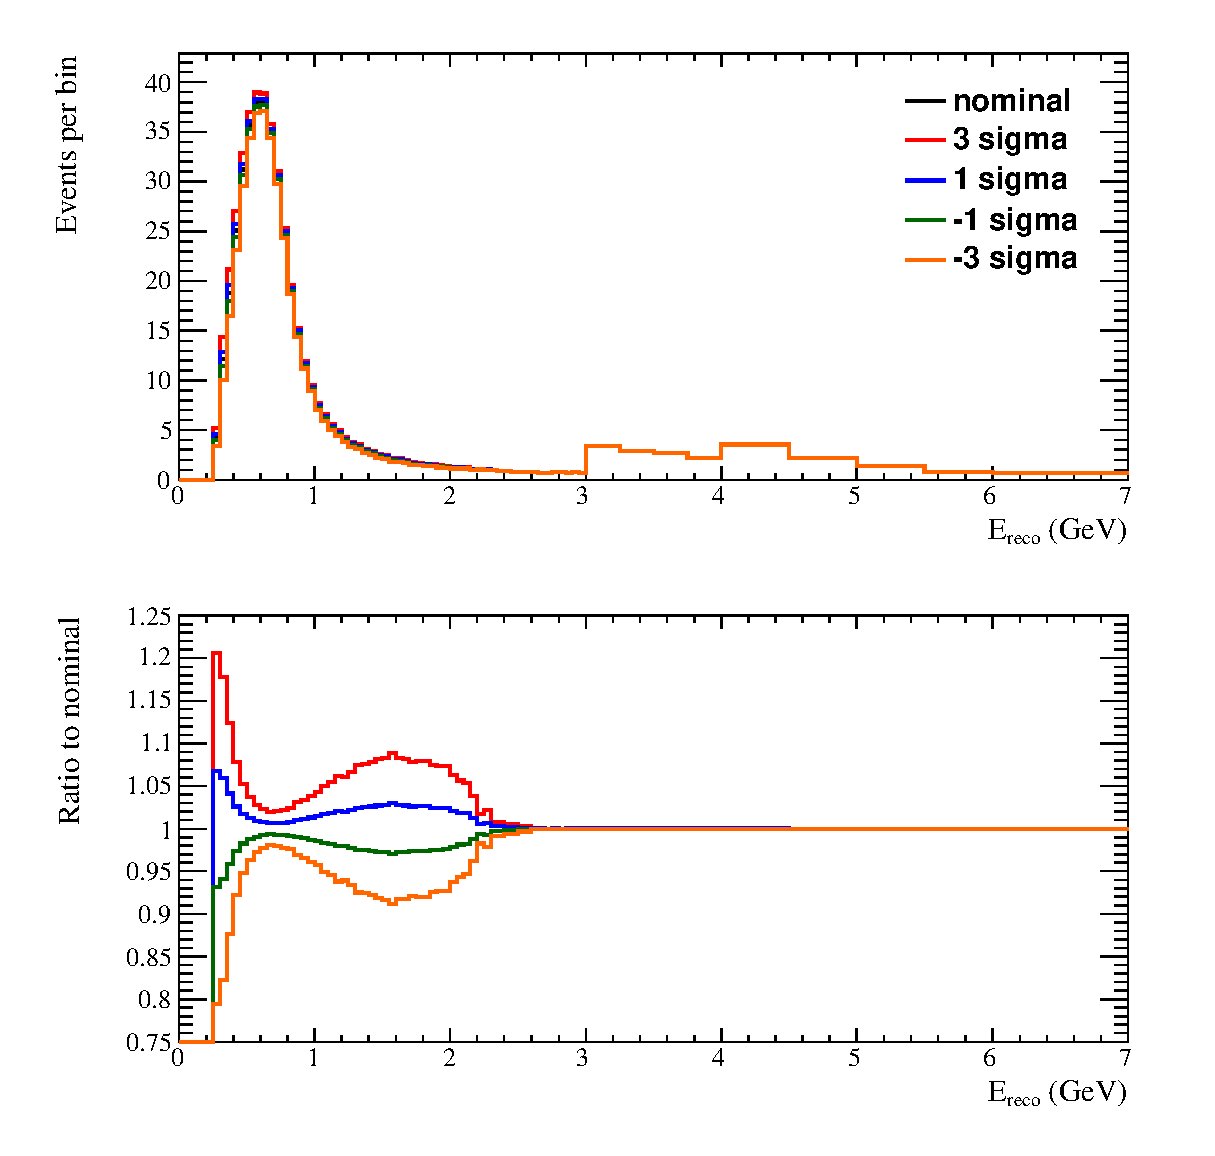
\includegraphics{../images/spectrum_tweaked/1sigma_unoscillated/ereco_twk_f_banffcc1pie0}}
\caption
{ Effect of $f_{21; t, r}^{banff}$ for no oscillations (all mixing angles set to 0). }
\label{fig:noosc_ereco_twk_f_banffcc1pie0}
\end{center}
\end{figure}
\clearpage

\begin{figure}
\begin{center}
\resizebox{14cm}{!}{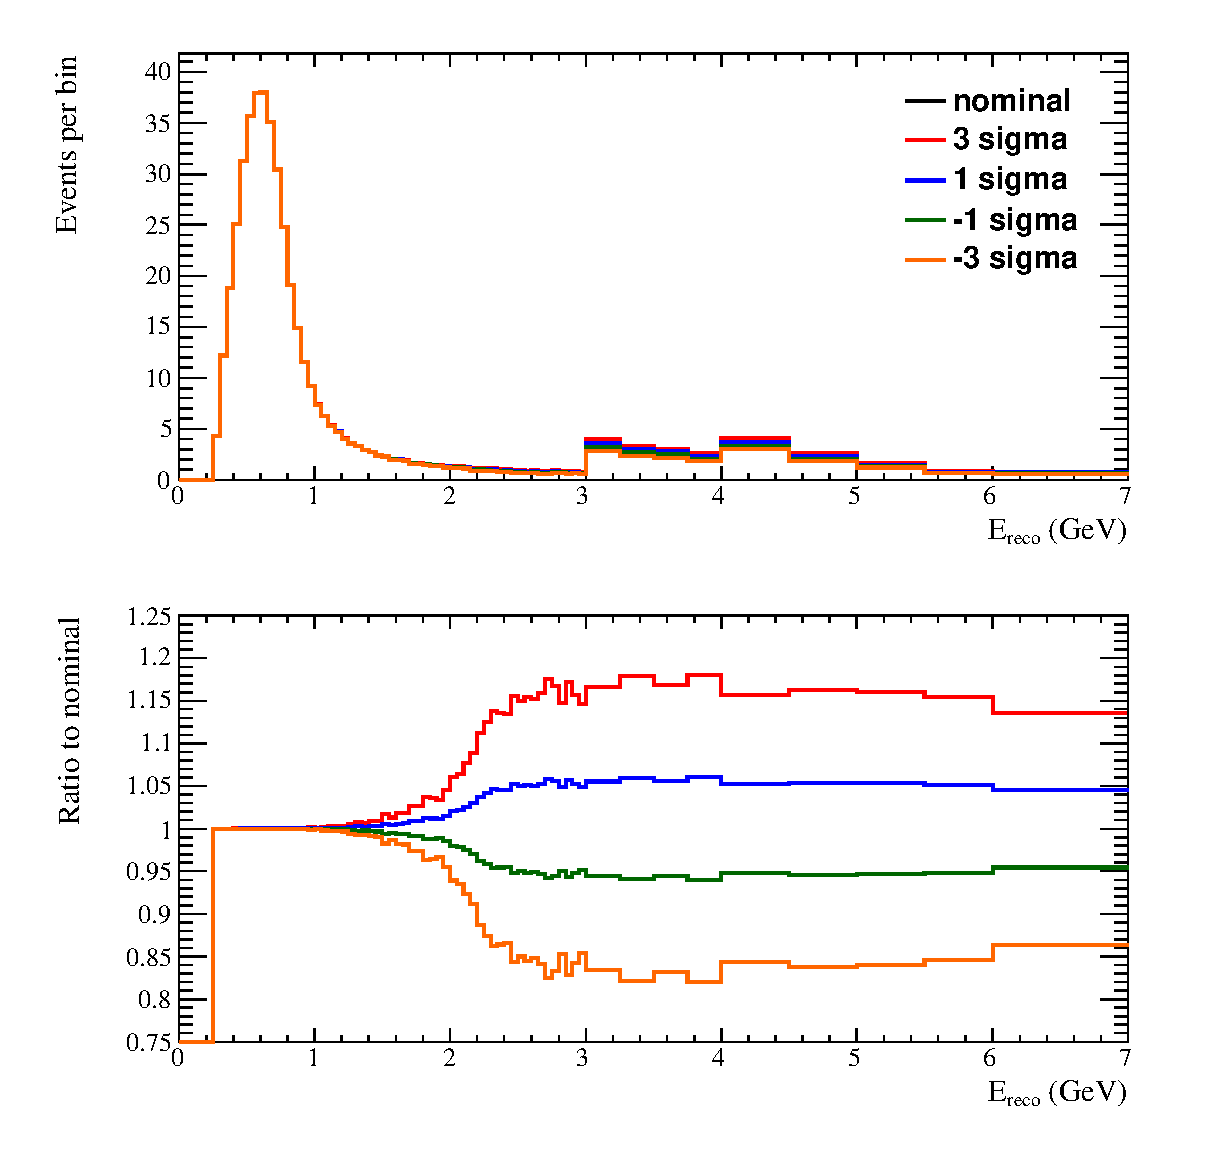
\includegraphics{../images/spectrum_tweaked/1sigma_unoscillated/ereco_twk_f_banffcc1pie1}}
\caption
{ Effect of $f_{22; t, r}^{banff}$ for no oscillations (all mixing angles set to 0). }
\label{fig:noosc_ereco_twk_f_banffcc1pie1}
\end{center}
\end{figure}
\clearpage

\begin{figure}
\begin{center}
\resizebox{14cm}{!}{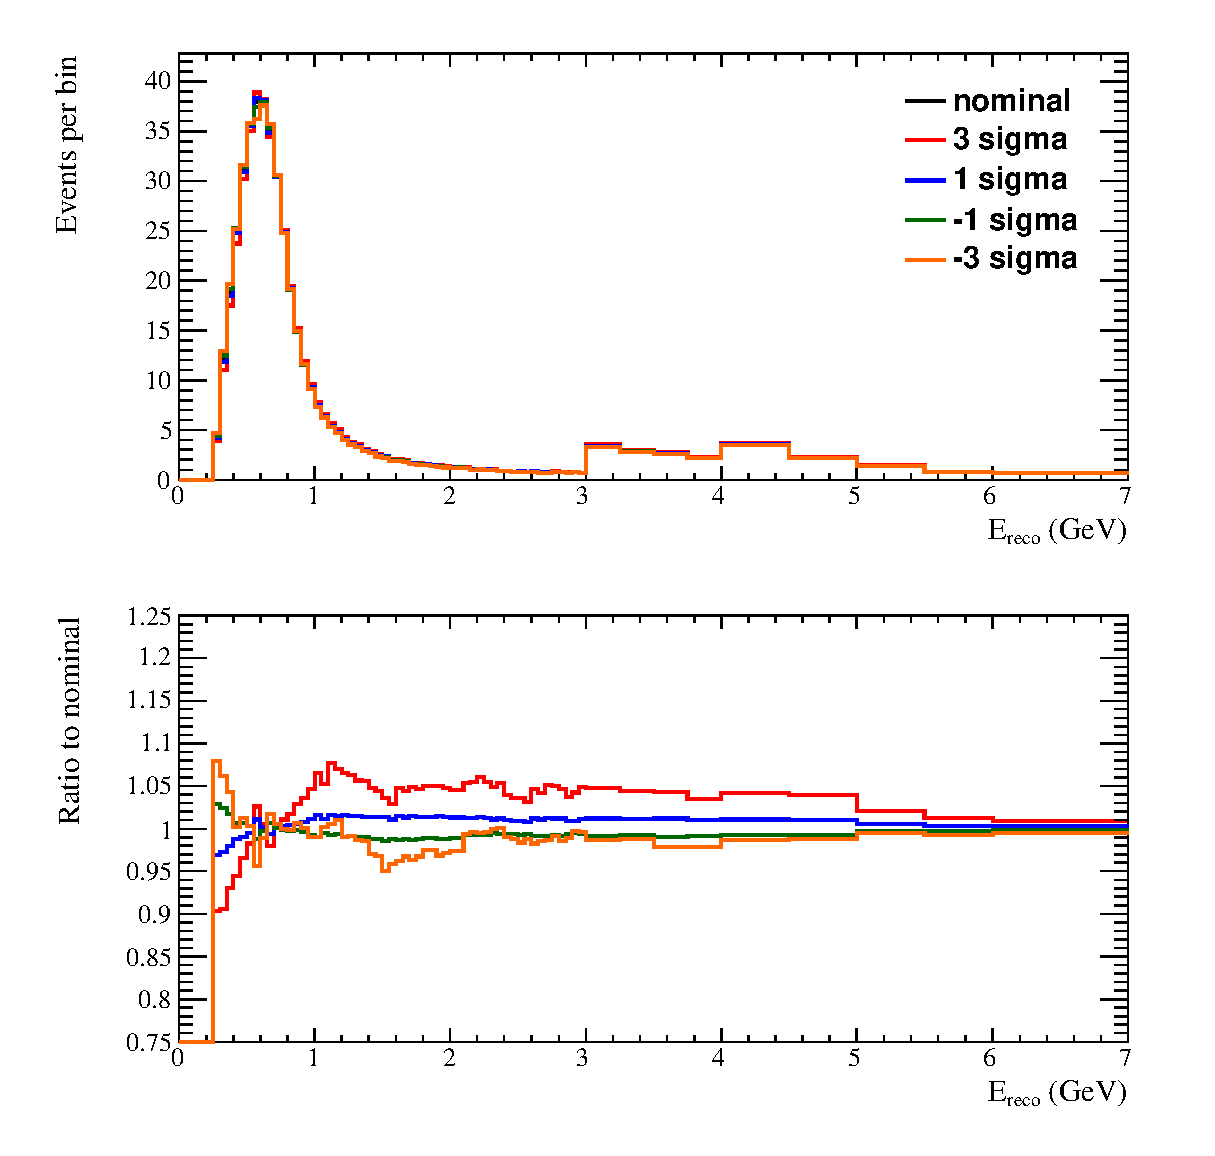
\includegraphics{../images/spectrum_tweaked/1sigma_unoscillated/ereco_twk_f_pfermi}}
\caption
{ Effect of $f_{pF; t, r}$ for no oscillations (all mixing angles set to 0). }
\label{fig:noosc_ereco_twk_f_pfermi}
\end{center}
\end{figure}
\clearpage

\begin{figure}
\begin{center}
\resizebox{14cm}{!}{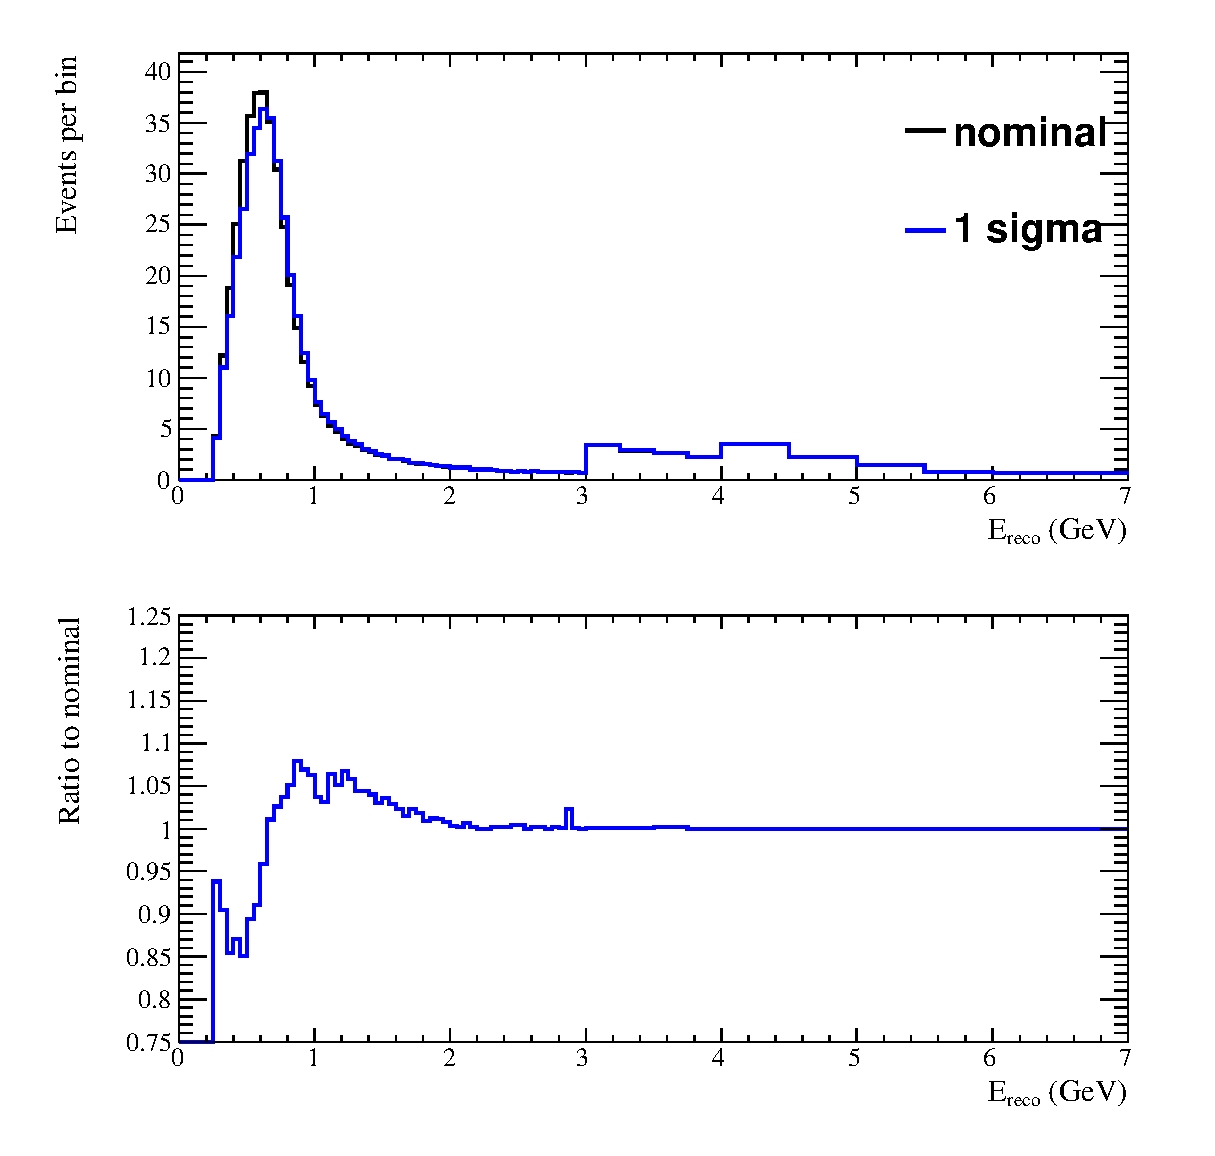
\includegraphics{../images/spectrum_tweaked/1sigma_unoscillated/ereco_twk_f_specfunc}}
\caption
{ Effect of $f_{SF; t, r}$ for no oscillations (all mixing angles set to 0). }
\label{fig:noosc_ereco_twk_f_specfunc}
\end{center}
\end{figure}
\clearpage

\begin{figure}
\begin{center}
\resizebox{14cm}{!}{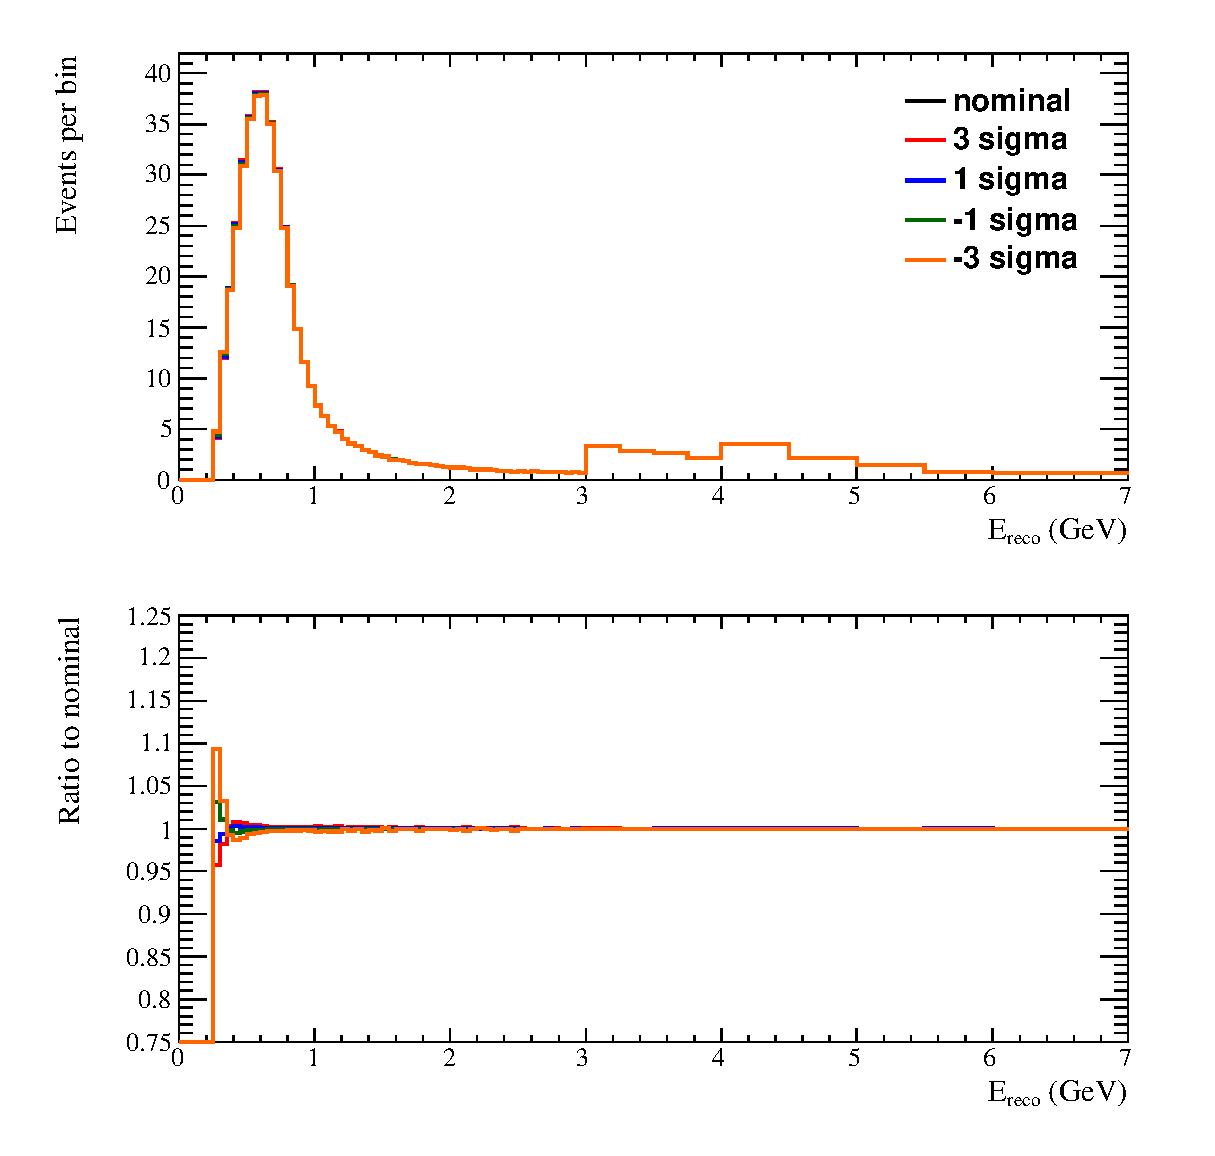
\includegraphics{../images/spectrum_tweaked/1sigma_unoscillated/ereco_twk_f_wshape}}
\caption
{ Effect of $f_{Wshape; t, r}$ for no oscillations (all mixing angles set to 0). }
\label{fig:noosc_ereco_twk_f_wshape}
\end{center}
\end{figure}
\clearpage

\begin{figure}
\begin{center}
\resizebox{14cm}{!}{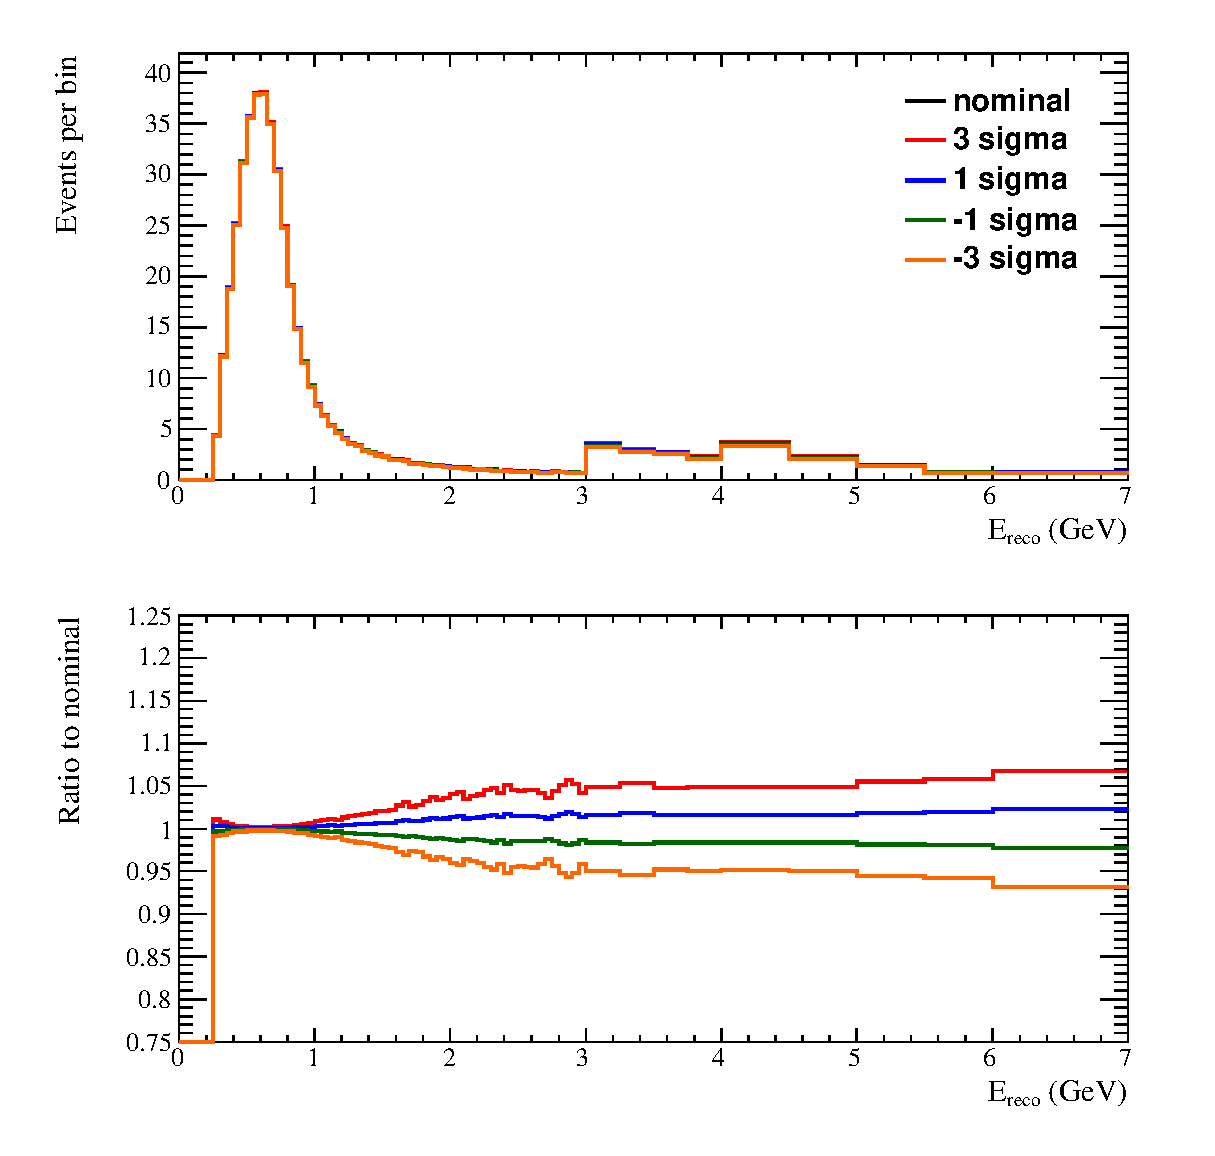
\includegraphics{../images/spectrum_tweaked/1sigma_unoscillated/ereco_twk_f_shapeCCoth}}
\caption
{ Effect of $f_{CCothShape; t, r}$ for no oscillations (all mixing angles set to 0). }
\label{fig:noosc_ereco_twk_f_shapeCCoth}
\end{center}
\end{figure}
\clearpage

\begin{figure}
\begin{center}
\resizebox{14cm}{!}{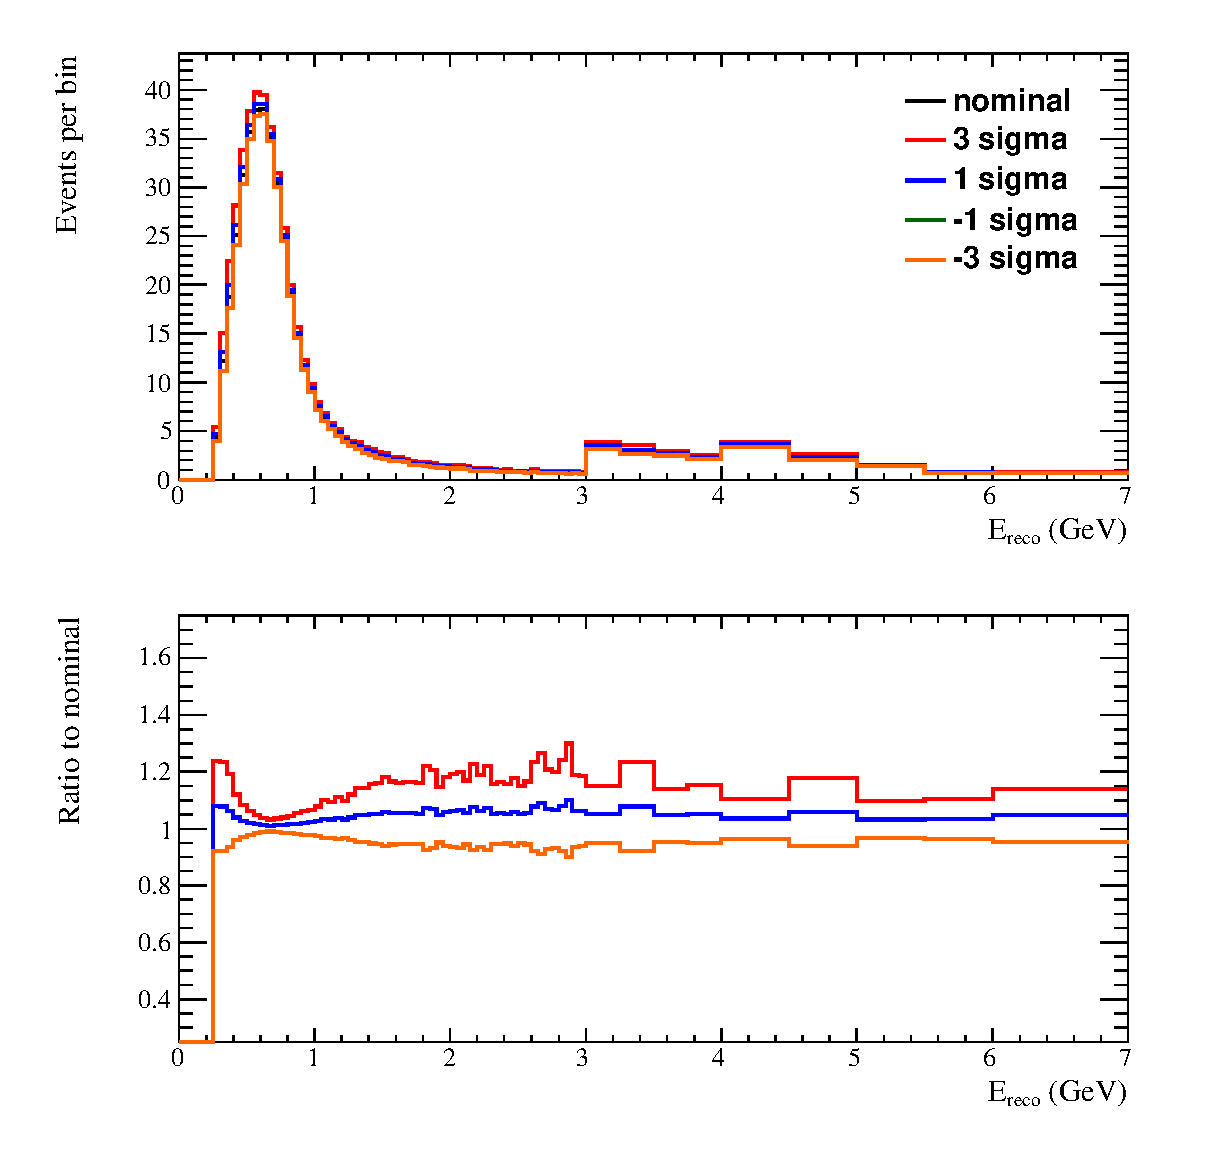
\includegraphics{../images/spectrum_tweaked/1sigma_unoscillated/ereco_twk_f_pilessdelta}}
\caption
{ Effect of $f_{\pi-less\Delta; t, r}$ for no oscillations (all mixing angles set to 0). }
\label{fig:noosc_ereco_twk_f_pilessdelta}
\end{center}
\end{figure}
\clearpage

\begin{figure}
\begin{center}
\resizebox{14cm}{!}{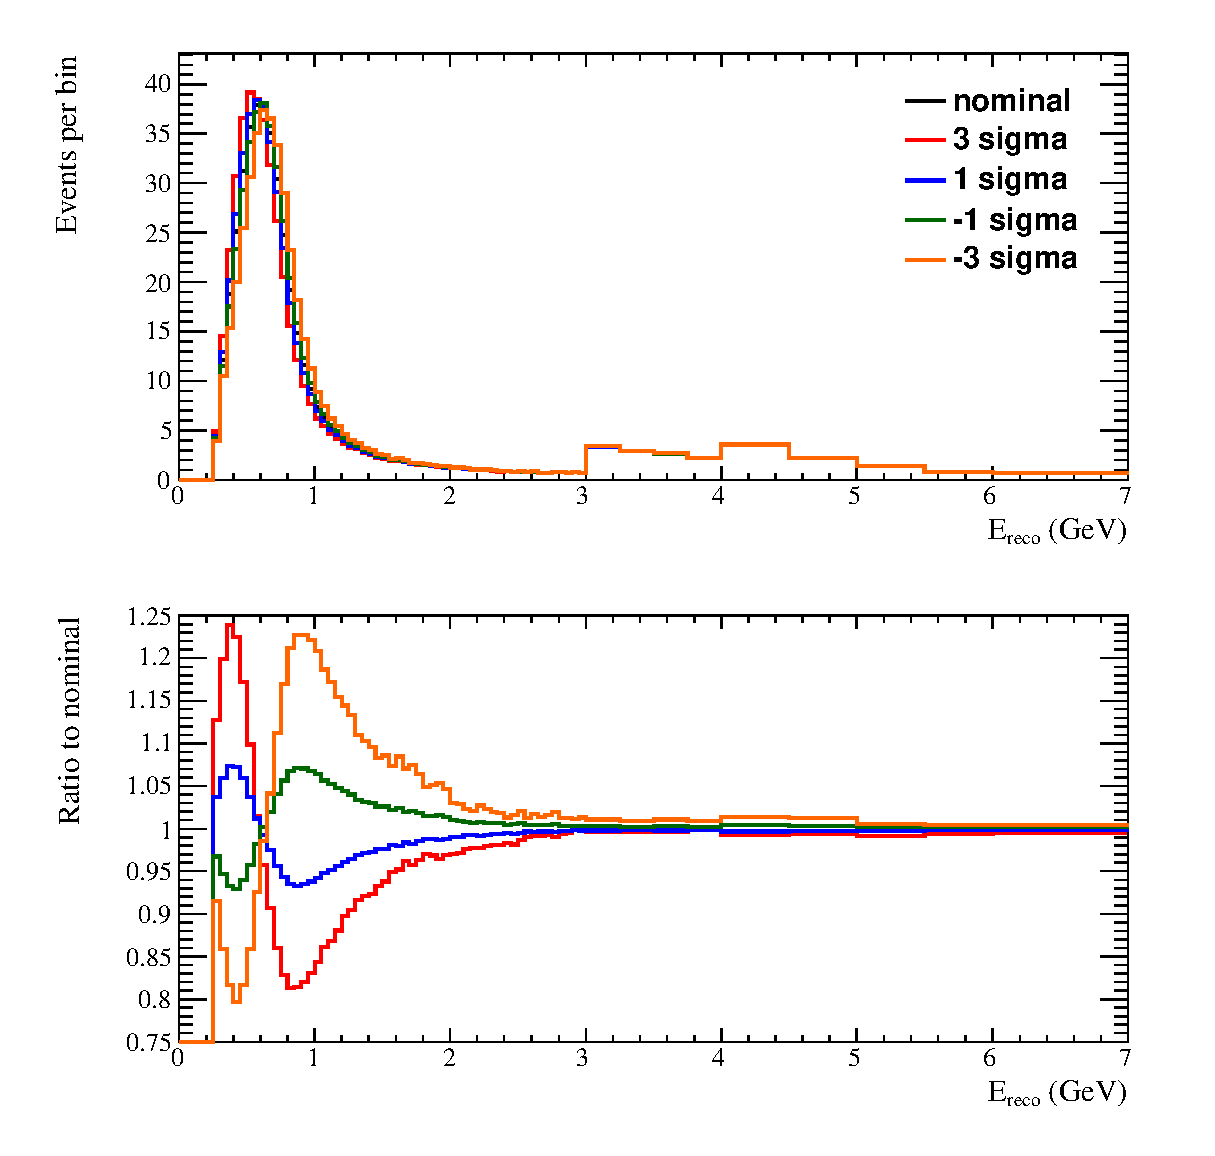
\includegraphics{../images/spectrum_tweaked/1sigma_unoscillated/ereco_twk_f_bindE}}
\caption
{ Effect of $f_{bindE; t, r}$ for no oscillations (all mixing angles set to 0). }
\label{fig:noosc_ereco_twk_f_bindE}
\end{center}
\end{figure}
\clearpage

\begin{figure}
\begin{center}
\resizebox{14cm}{!}{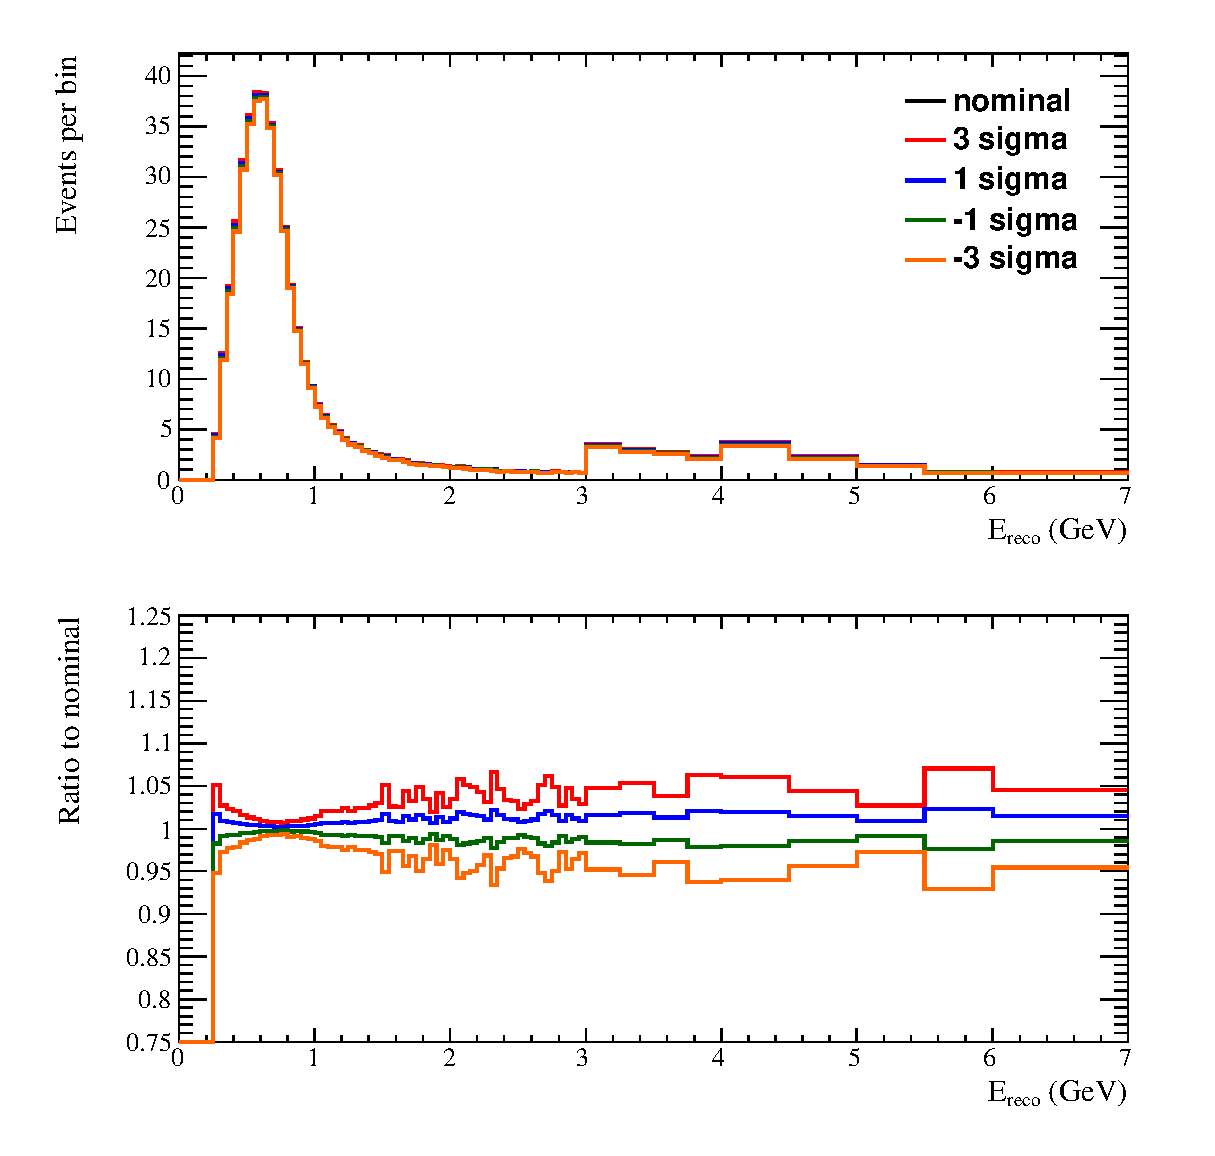
\includegraphics{../images/spectrum_tweaked/1sigma_unoscillated/ereco_twk_f_norm_cccoh}}
\caption
{ Effect of $f_{CCcoh; t}$ for no oscillations (all mixing angles set to 0). }
\label{fig:noosc_ereco_twk_f_norm_cccoh}
\end{center}
\end{figure}
\clearpage

\begin{figure}
\begin{center}
\resizebox{14cm}{!}{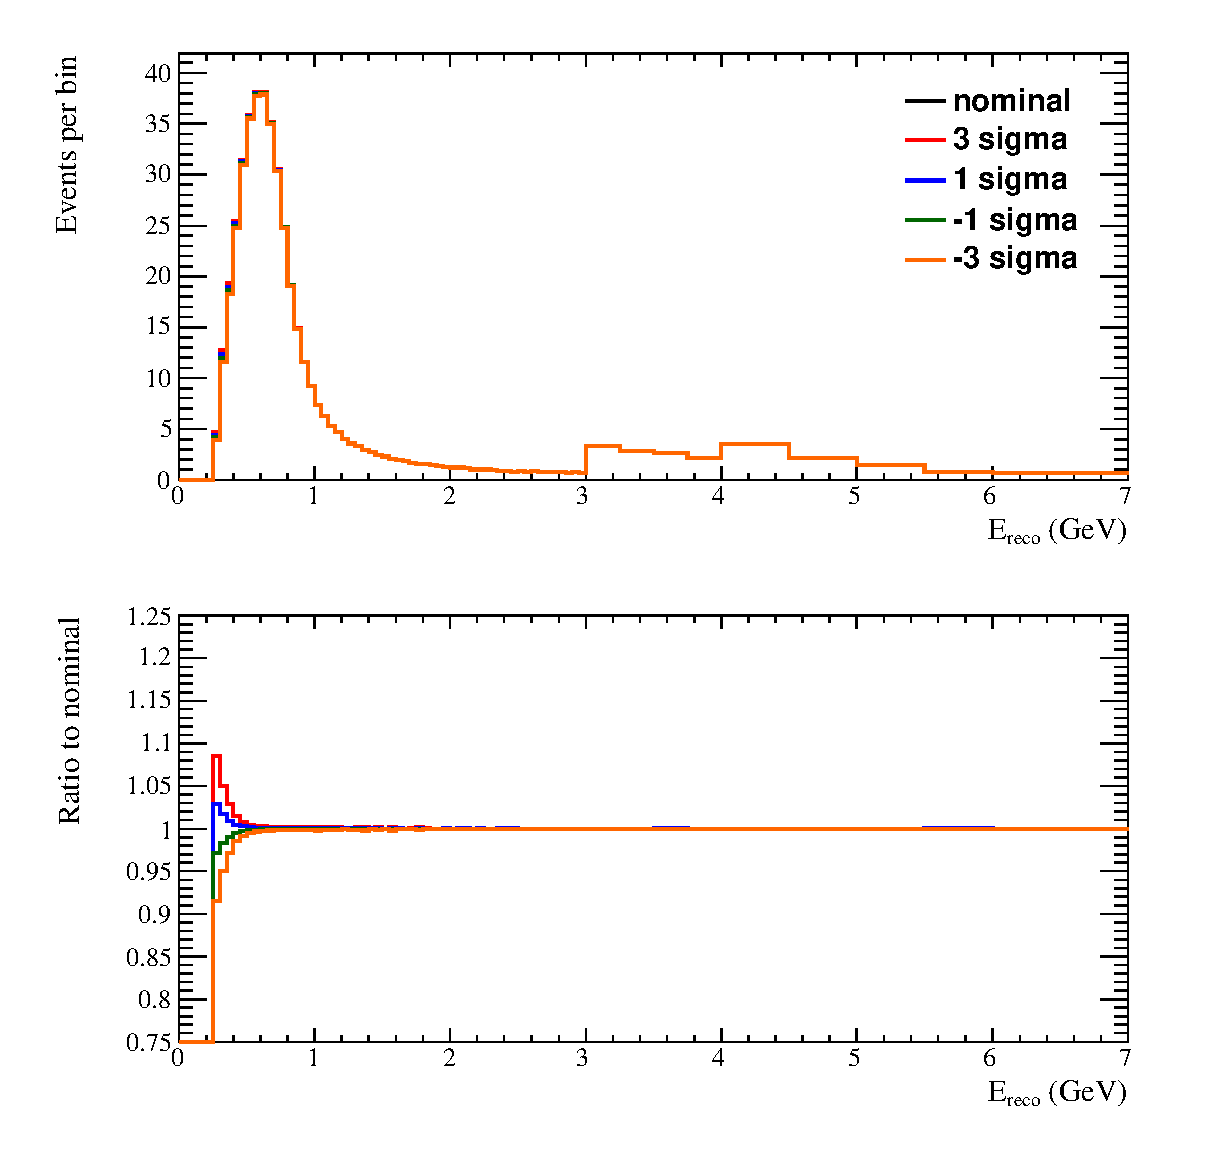
\includegraphics{../images/spectrum_tweaked/1sigma_unoscillated/ereco_twk_f_norm_nc1piC}}
\caption
{ Effect of $f_{NC1\pi^\pm; t}$ for no oscillations (all mixing angles set to 0). }
\label{fig:noosc_ereco_twk_f_norm_nc1piC}
\end{center}
\end{figure}
\clearpage

\begin{figure}
\begin{center}
\resizebox{14cm}{!}{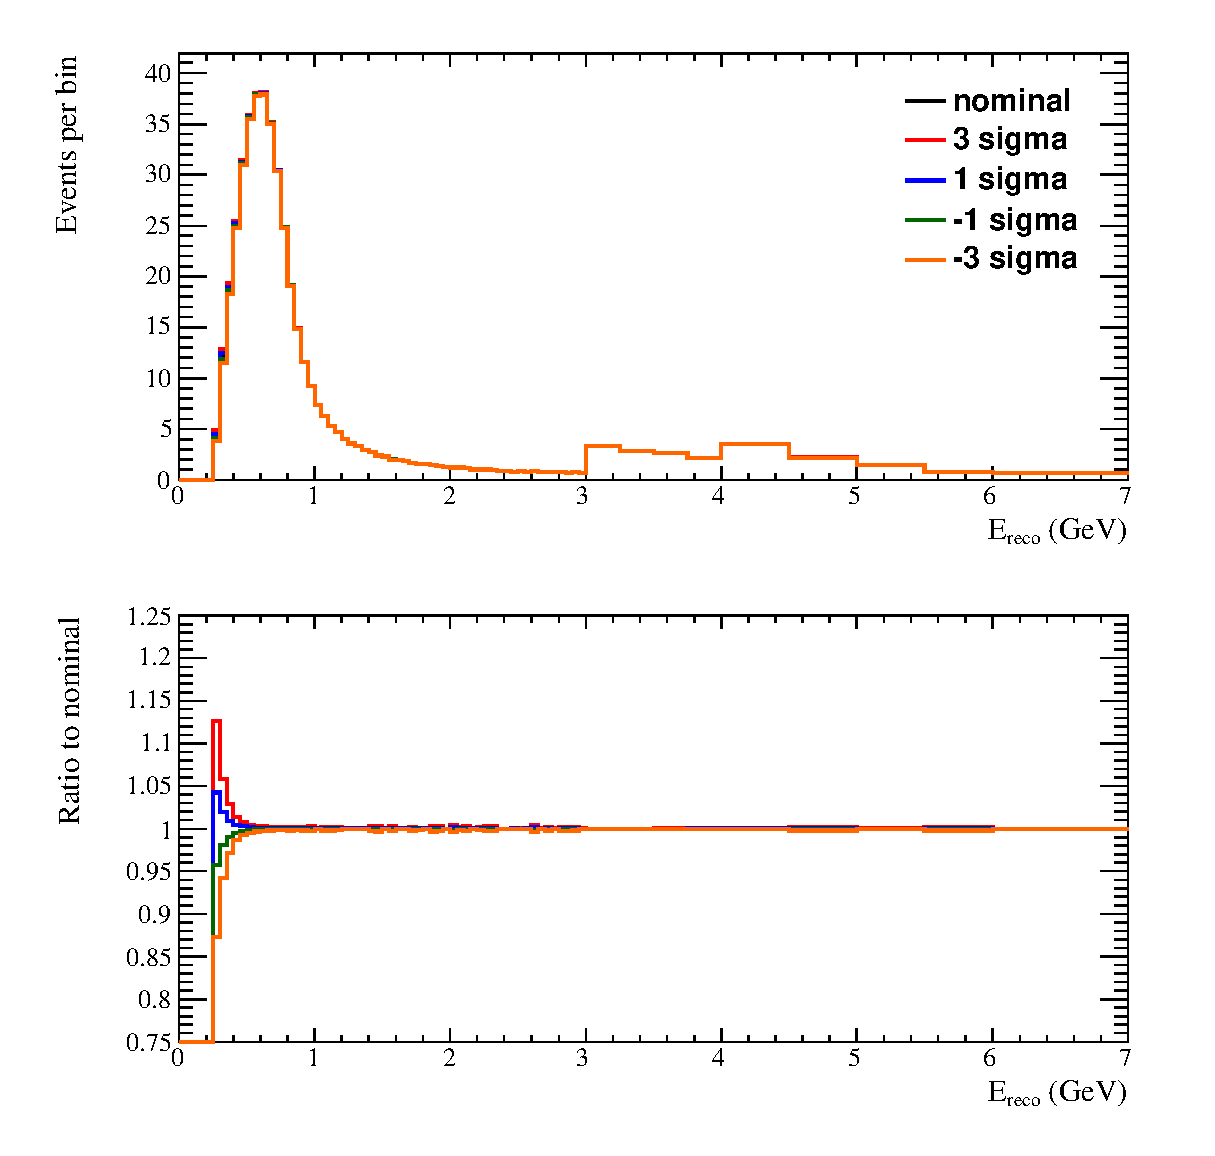
\includegraphics{../images/spectrum_tweaked/1sigma_unoscillated/ereco_twk_f_norm_ncoth}}
\caption
{ Effect of $f_{NCoth; t}$ for no oscillations (all mixing angles set to 0). }
\label{fig:noosc_ereco_twk_f_norm_ncoth}
\end{center}
\end{figure}
\clearpage

\begin{figure}
\begin{center}
\resizebox{14cm}{!}{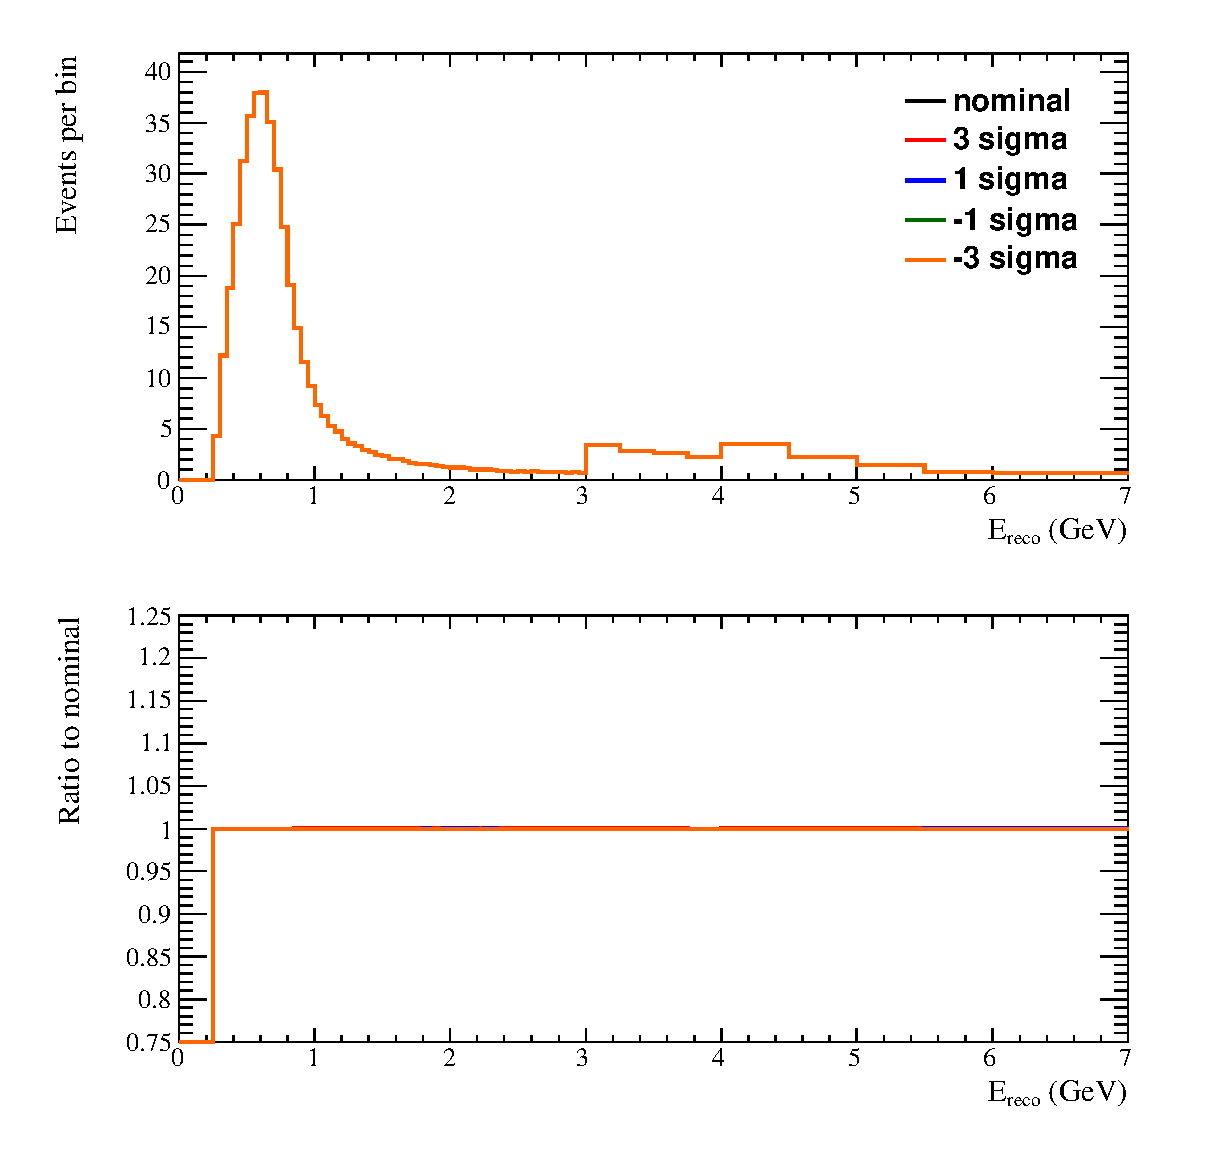
\includegraphics{../images/spectrum_tweaked/1sigma_unoscillated/ereco_twk_f_norm_nuetonumu}}
\caption
{ Effect of $f_{CC\nu_e; t}$ for no oscillations (all mixing angles set to 0). }
\label{fig:noosc_ereco_twk_f_norm_nuetonumu}
\end{center}
\end{figure}
\clearpage

\begin{figure}
\begin{center}
\resizebox{14cm}{!}{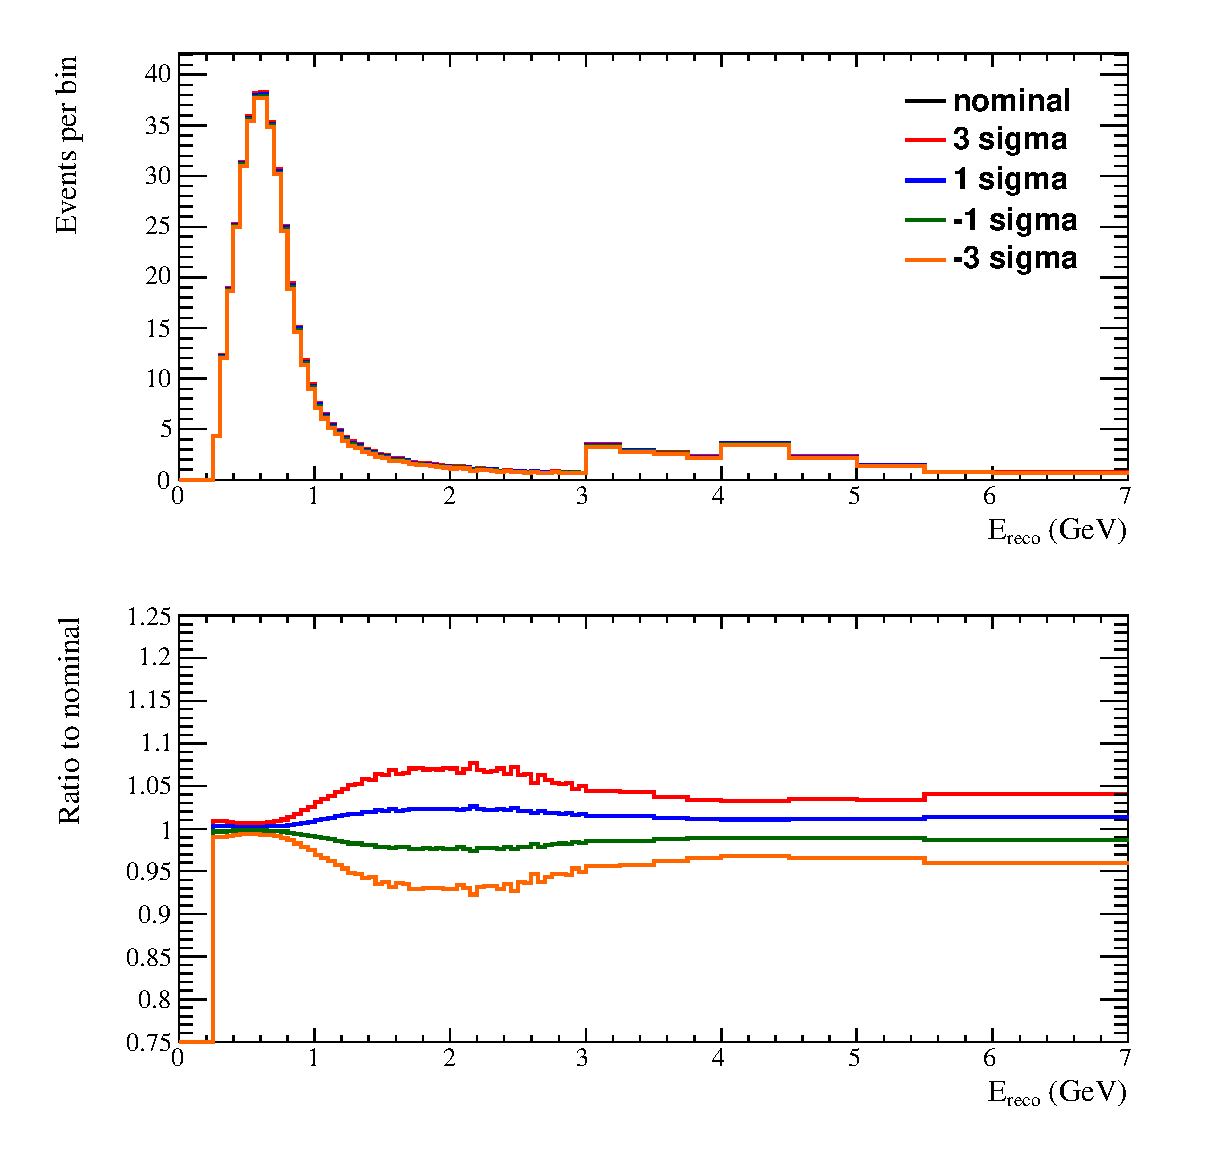
\includegraphics{../images/spectrum_tweaked/1sigma_unoscillated/ereco_twk_f_norm_antinutonu}}
\caption
{ Effect of $f_{CC\bar{\nu}; t}$ for no oscillations (all mixing angles set to 0). }
\label{fig:noosc_ereco_twk_f_norm_antinutonu}
\end{center}
\end{figure}
\clearpage

\begin{figure}
\begin{center}
\resizebox{14cm}{!}{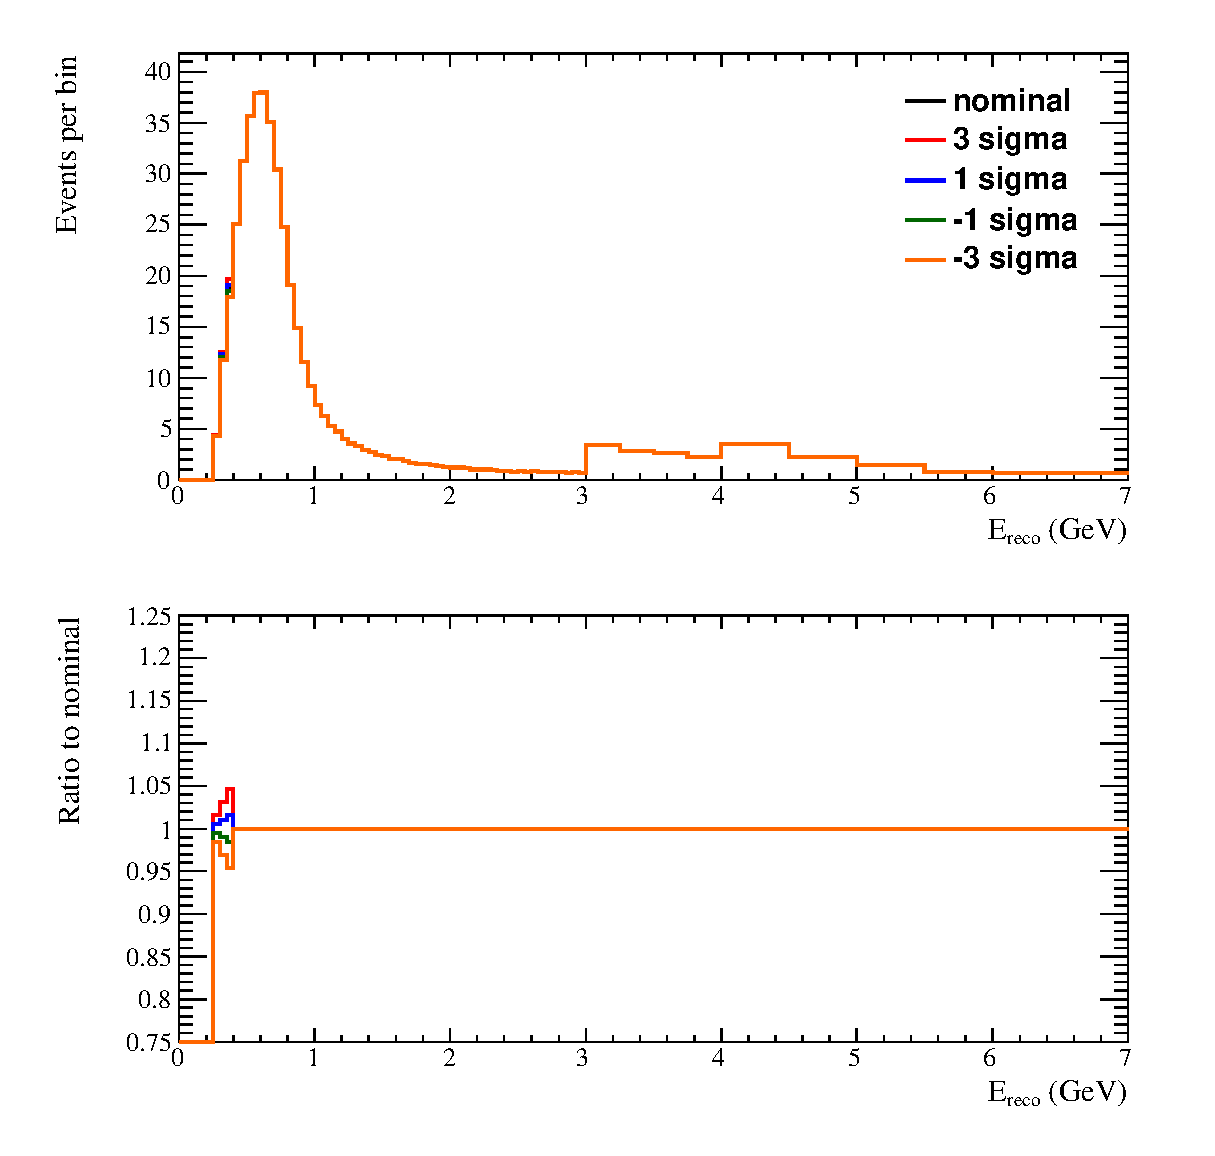
\includegraphics{../images/spectrum_tweaked/1sigma_unoscillated/ereco_twk_f_skdetfsi000}}
\caption
{ Effect of $f_{0; r}^{SK+FSI}$ for no oscillations (all mixing angles set to 0). }
\label{fig:noosc_ereco_twk_f_skdetfsi000}
\end{center}
\end{figure}
\clearpage

\begin{figure}
\begin{center}
\resizebox{14cm}{!}{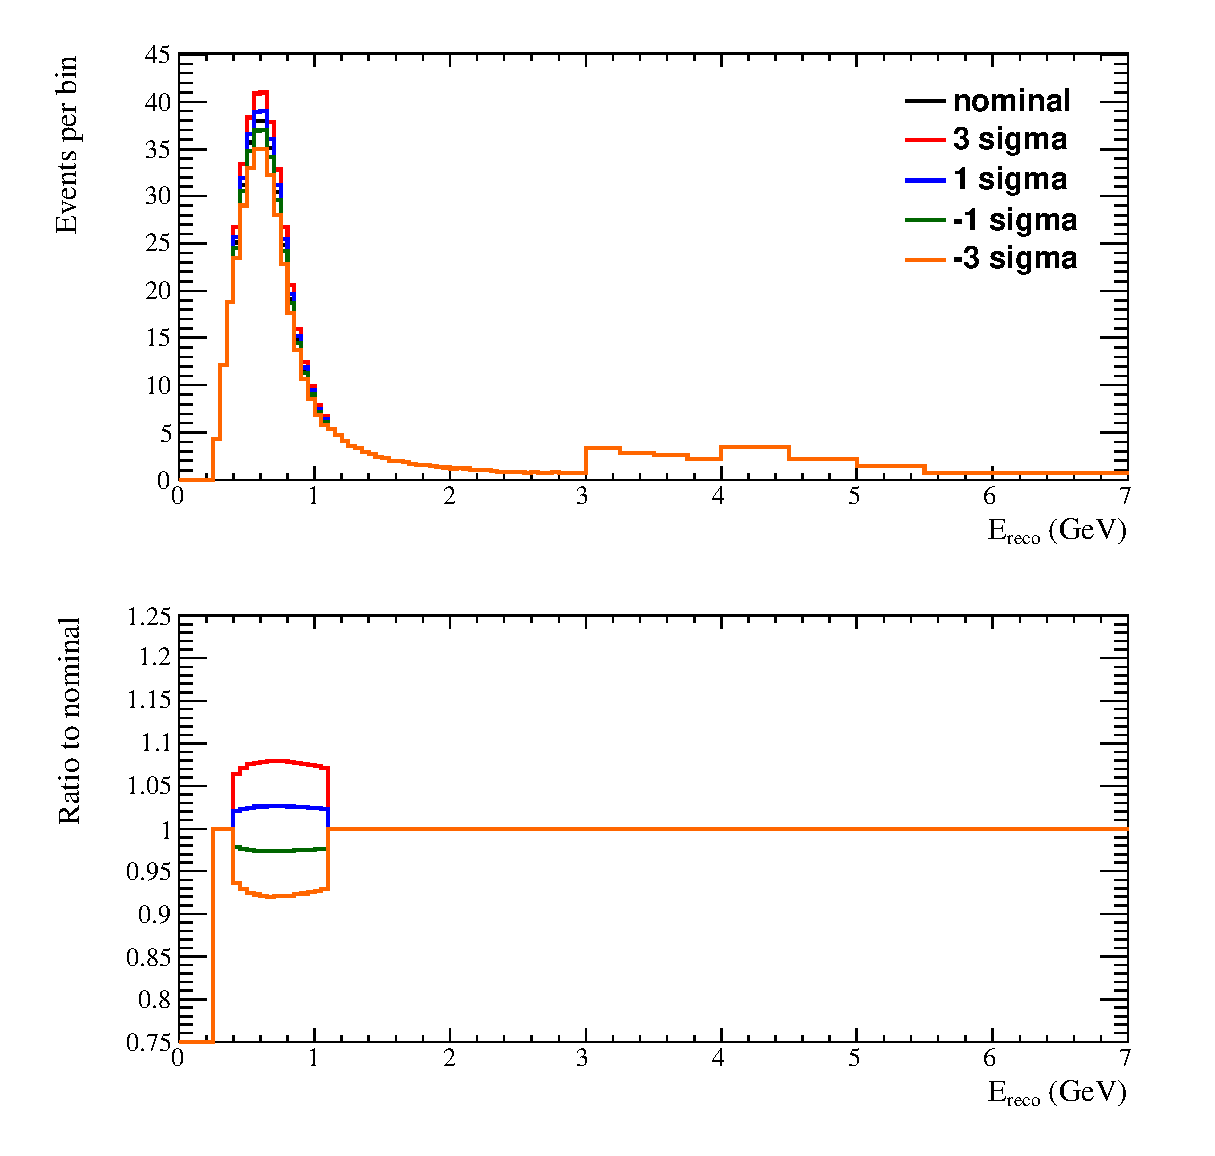
\includegraphics{../images/spectrum_tweaked/1sigma_unoscillated/ereco_twk_f_skdetfsi001}}
\caption
{ Effect of $f_{1; r}^{SK+FSI}$ for no oscillations (all mixing angles set to 0). }
\label{fig:noosc_ereco_twk_f_skdetfsi001}
\end{center}
\end{figure}
\clearpage

\begin{figure}
\begin{center}
\resizebox{14cm}{!}{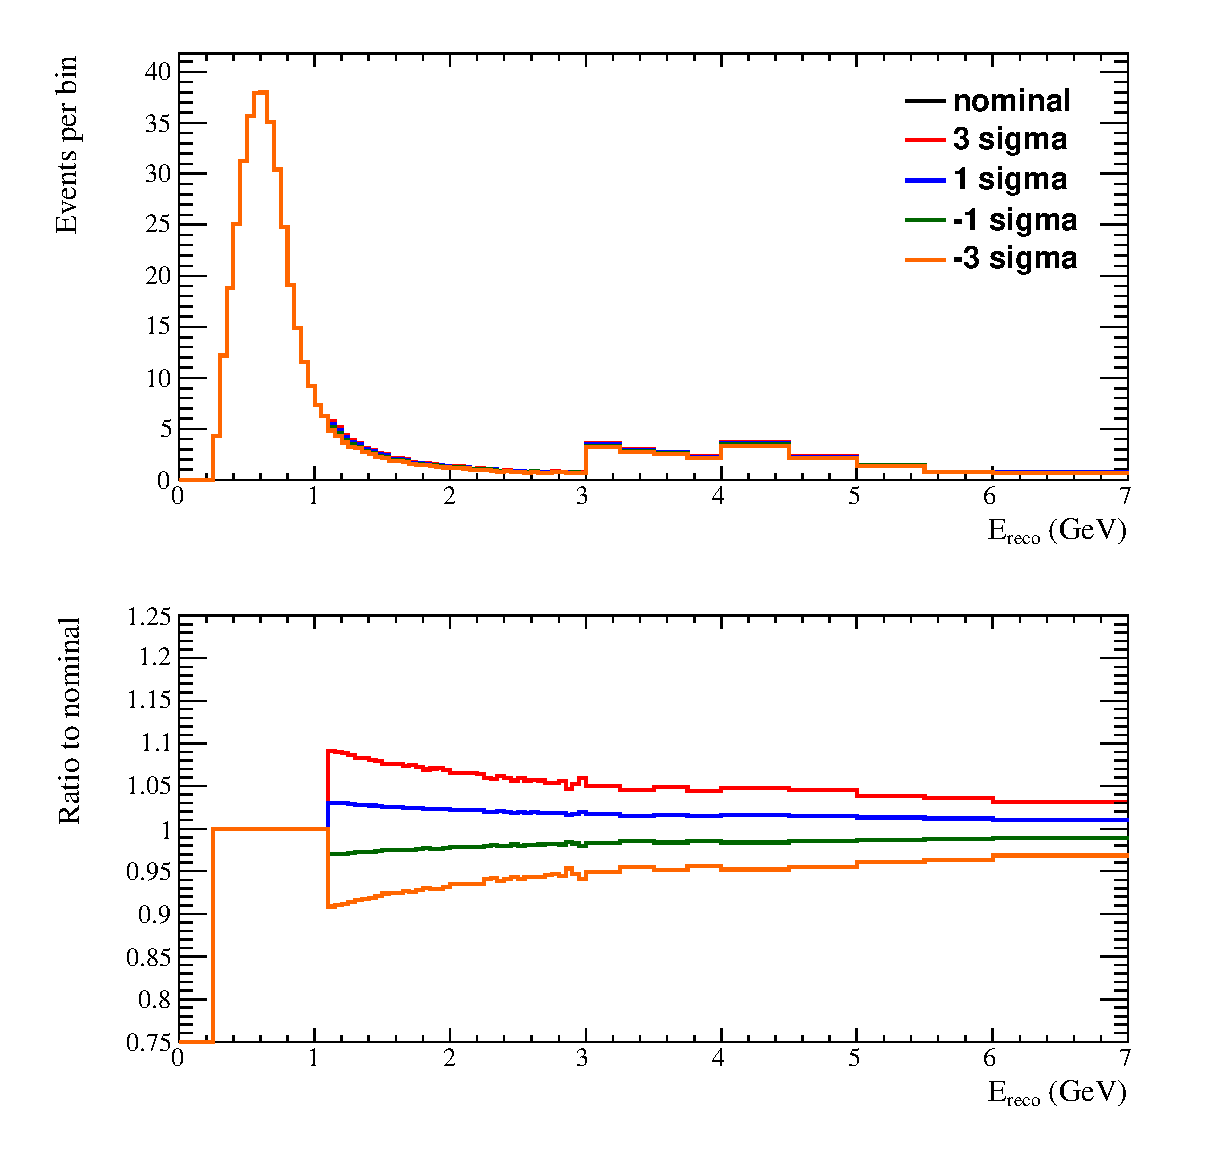
\includegraphics{../images/spectrum_tweaked/1sigma_unoscillated/ereco_twk_f_skdetfsi002}}
\caption
{ Effect of $f_{2; r}^{SK+FSI}$ for no oscillations (all mixing angles set to 0). }
\label{fig:noosc_ereco_twk_f_skdetfsi002}
\end{center}
\end{figure}
\clearpage

\begin{figure}
\begin{center}
\resizebox{14cm}{!}{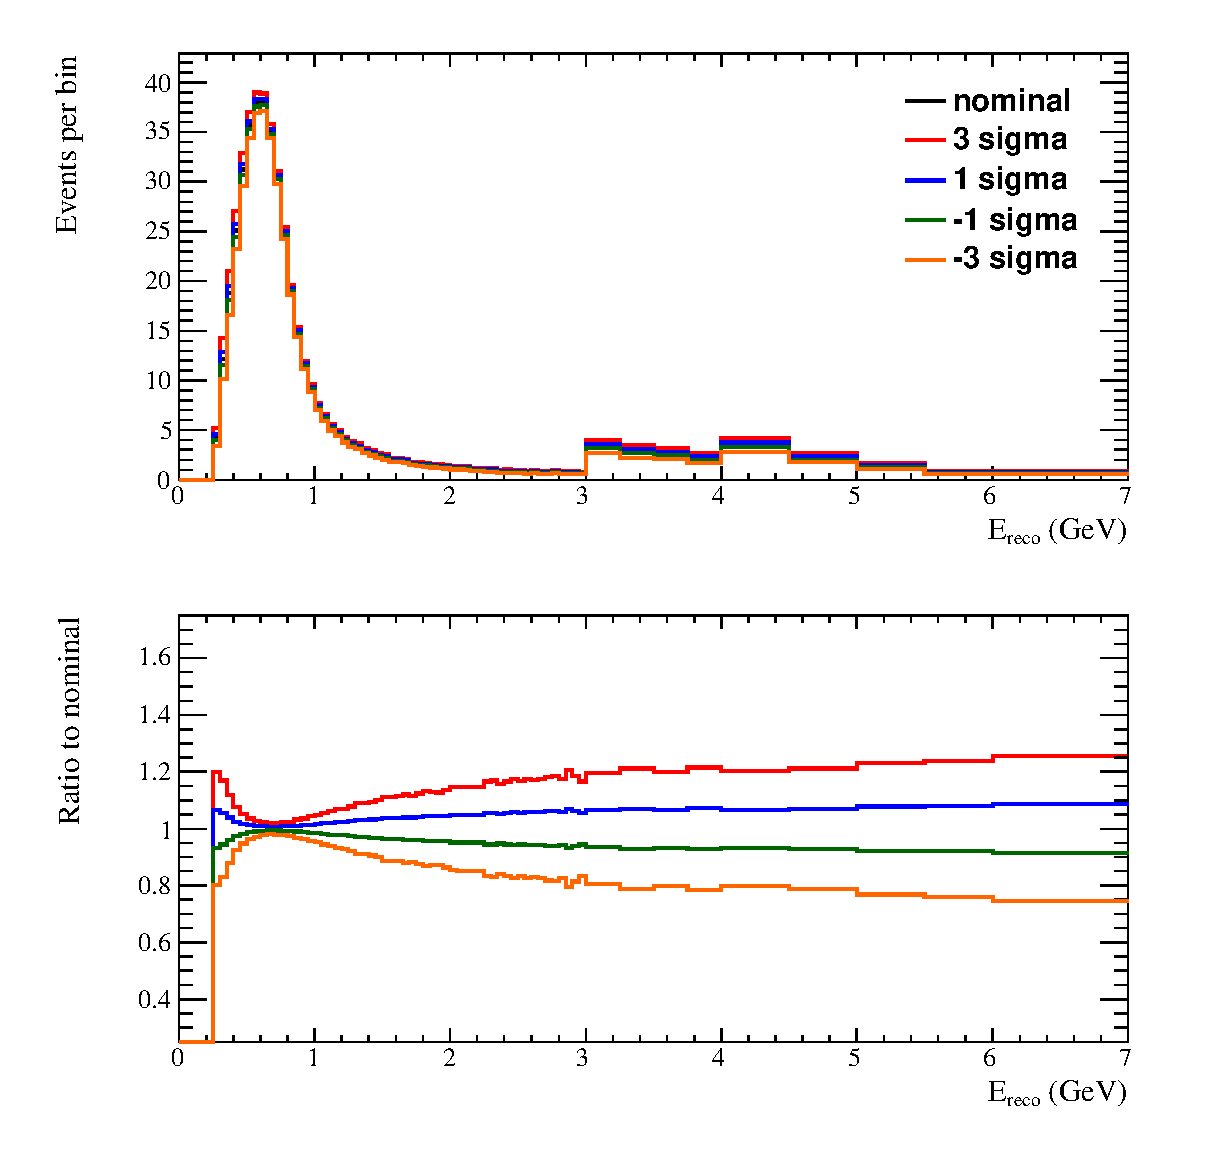
\includegraphics{../images/spectrum_tweaked/1sigma_unoscillated/ereco_twk_f_skdetfsi003}}
\caption
{ Effect of $f_{3; r}^{SK+FSI}$ for no oscillations (all mixing angles set to 0). }
\label{fig:noosc_ereco_twk_f_skdetfsi003}
\end{center}
\end{figure}
\clearpage

\begin{figure}
\begin{center}
\resizebox{14cm}{!}{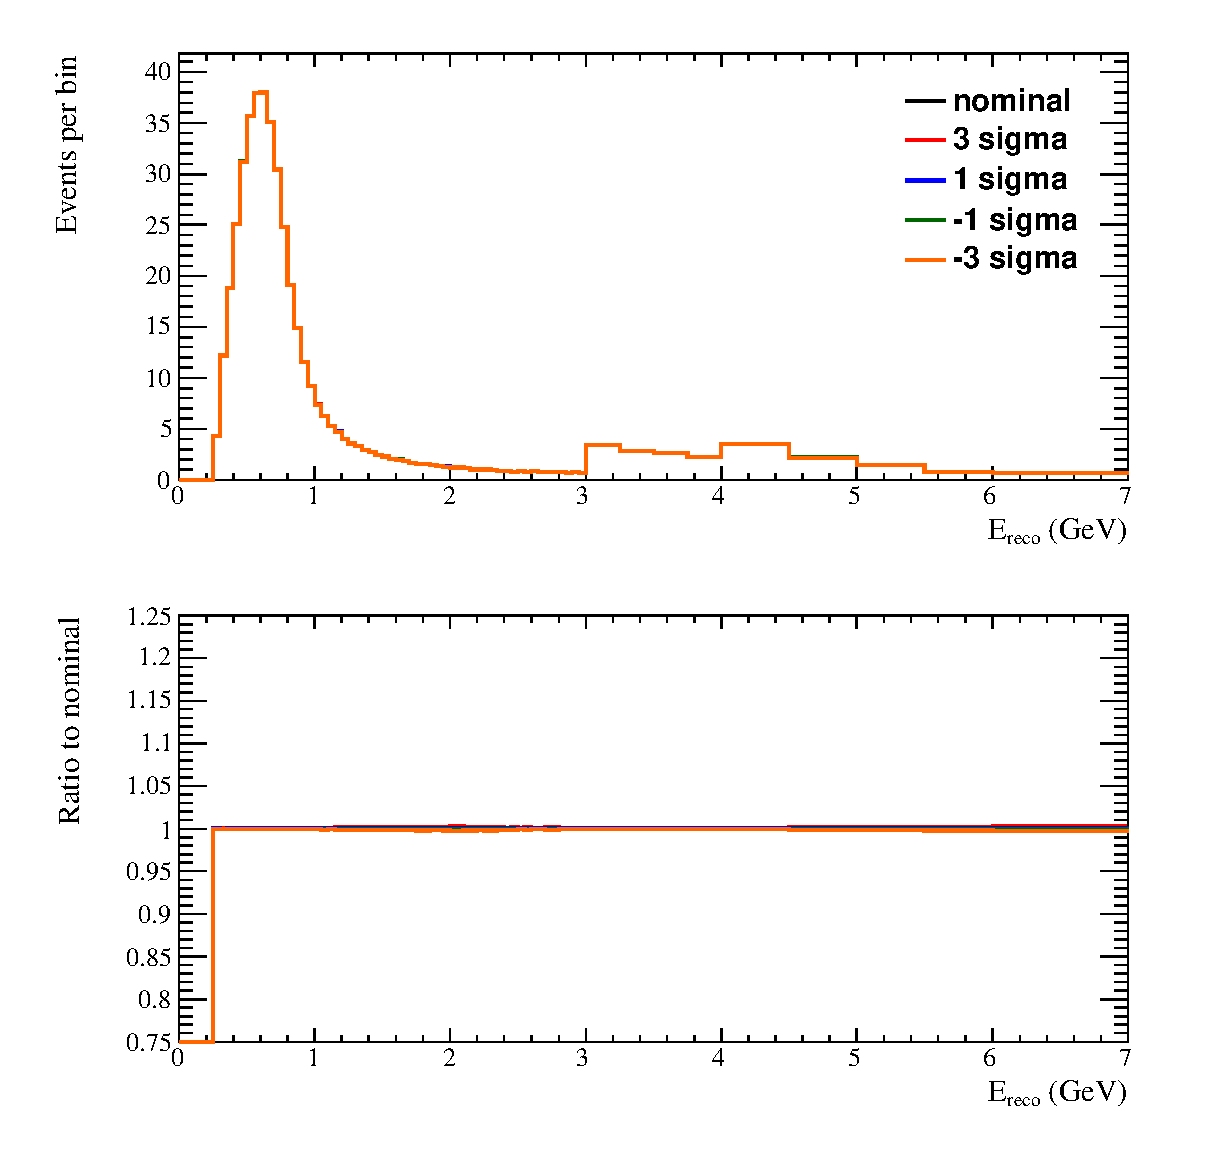
\includegraphics{../images/spectrum_tweaked/1sigma_unoscillated/ereco_twk_f_skdetfsi004}}
\caption
{ Effect of $f_{4; r}^{SK+FSI}$ for no oscillations (all mixing angles set to 0). }
\label{fig:noosc_ereco_twk_f_skdetfsi004}
\end{center}
\end{figure}
\clearpage

\begin{figure}
\begin{center}
\resizebox{14cm}{!}{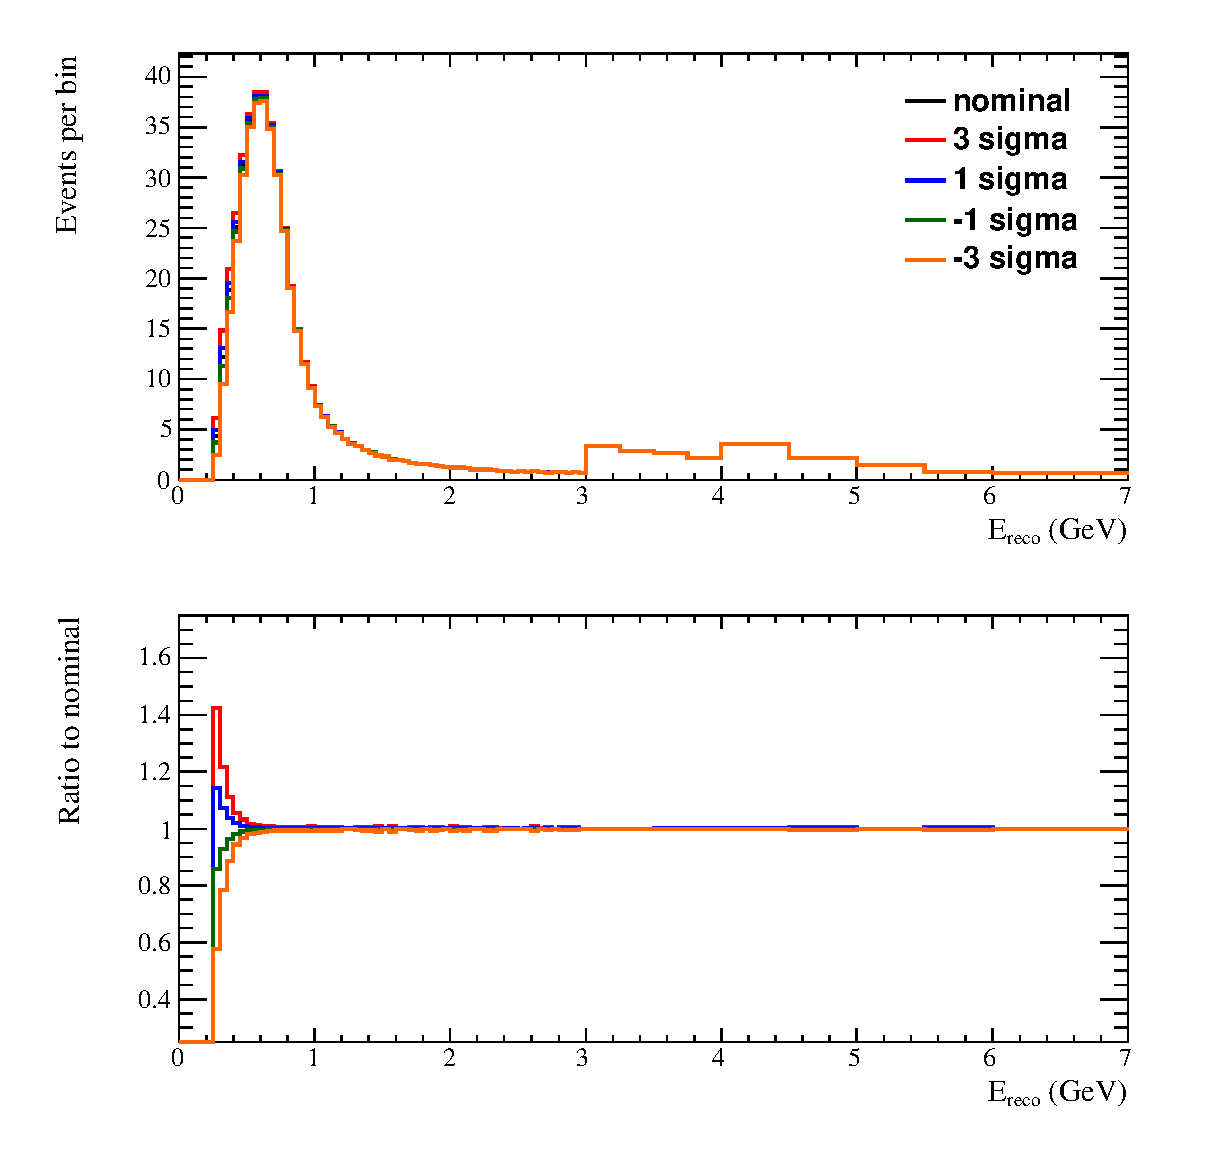
\includegraphics{../images/spectrum_tweaked/1sigma_unoscillated/ereco_twk_f_skdetfsi005}}
\caption
{ Effect of $f_{5; r}^{SK+FSI}$ for no oscillations (all mixing angles set to 0). }
\label{fig:noosc_ereco_twk_f_skdetfsi005}
\end{center}
\end{figure}
\clearpage



\begin{figure}
\begin{center}
\resizebox{14cm}{!}{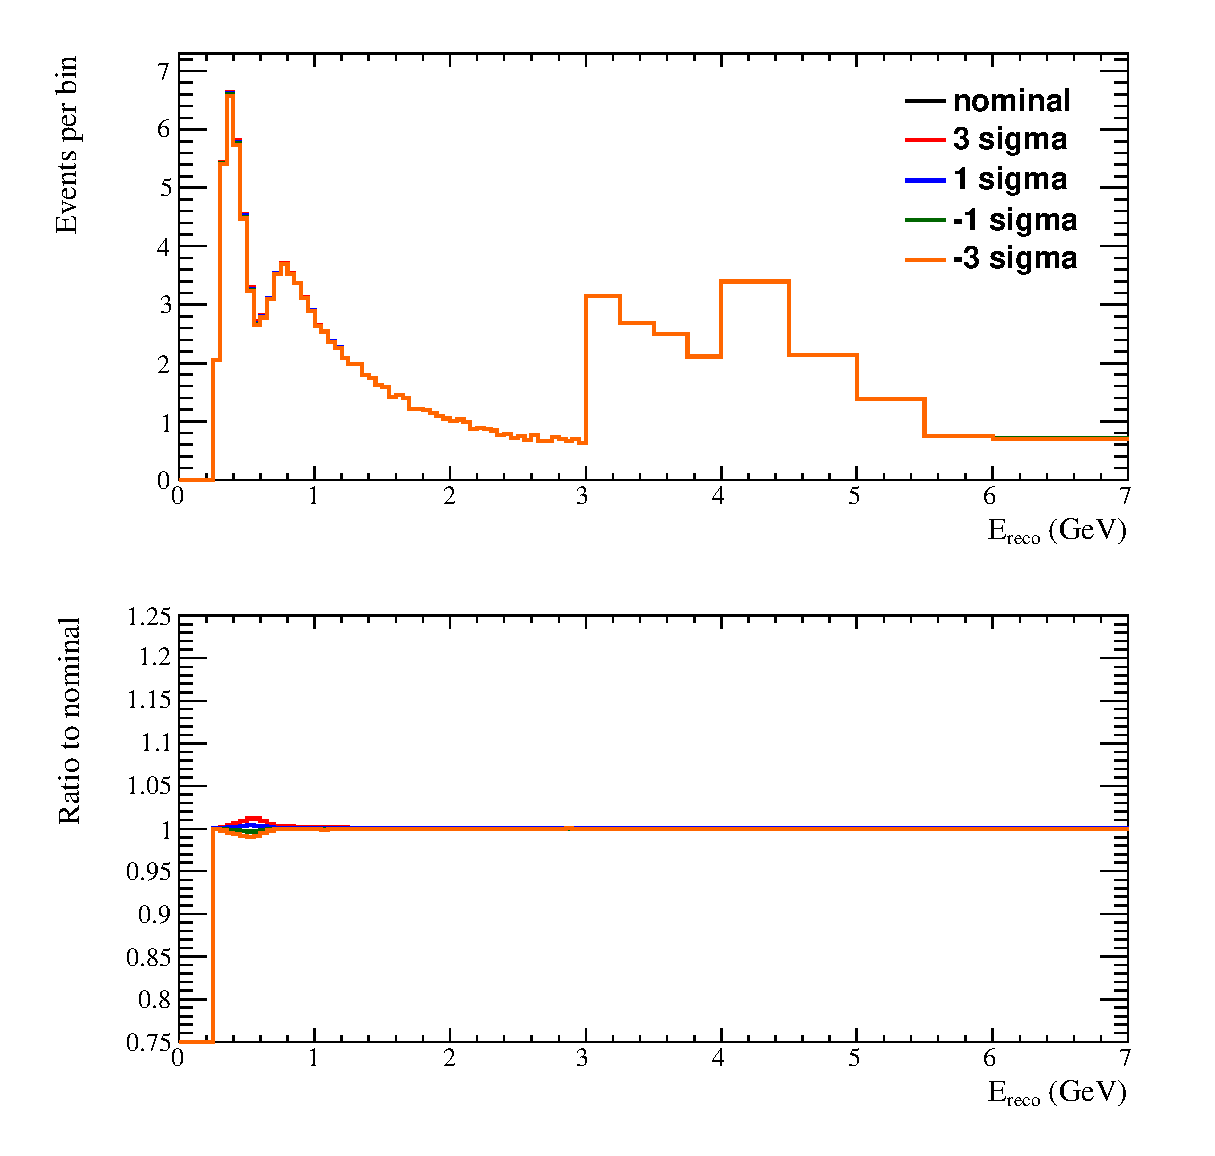
\includegraphics{../images/spectrum_tweaked/1sigma_oscillated/ereco_twk_sinsqtheta13}}
\caption
{ Effect of $\sin^2(\theta_{13})$ for 3 flavour oscillations, using oscillation parameters:  $\sin^2\theta_{12} = $0.306; $\sin^2\theta_{13} = $0.0251; $\sin^2\theta_{23} = $0.5; $\delta_{CP} = $        0; $\Delta m^2_{21} = $    7.5e-05 eV$^2$/c$^4$; $|\Delta m^2_{32}| = $    0.0024 eV$^2$/c$^4$. }
\label{fig:osc_ereco_twk_sinsqtheta13}
\end{center}
\end{figure}
\clearpage

\begin{figure}
\begin{center}
\resizebox{14cm}{!}{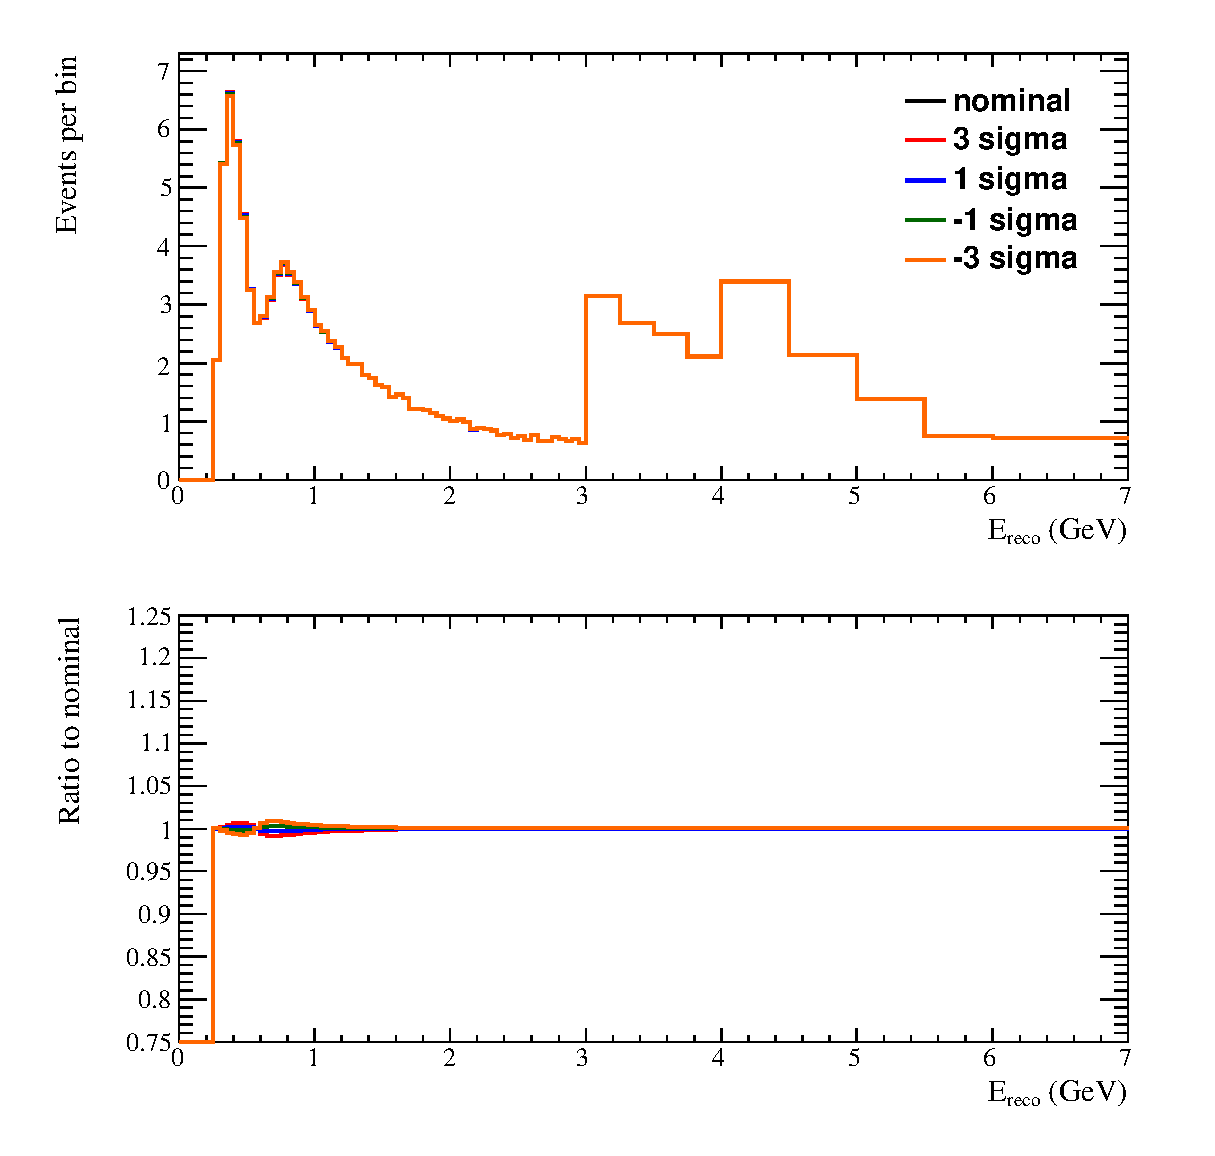
\includegraphics{../images/spectrum_tweaked/1sigma_oscillated/ereco_twk_sinsqtheta12}}
\caption
{ Effect of $\sin^2(\theta_{12})$ for 3 flavour oscillations, using oscillation parameters:  $\sin^2\theta_{12} = $0.306; $\sin^2\theta_{13} = $0.0251; $\sin^2\theta_{23} = $0.5; $\delta_{CP} = $        0; $\Delta m^2_{21} = $    7.5e-05 eV$^2$/c$^4$; $|\Delta m^2_{32}| = $    0.0024 eV$^2$/c$^4$. }
\label{fig:osc_ereco_twk_sinsqtheta12}
\end{center}
\end{figure}
\clearpage

\begin{figure}
\begin{center}
\resizebox{14cm}{!}{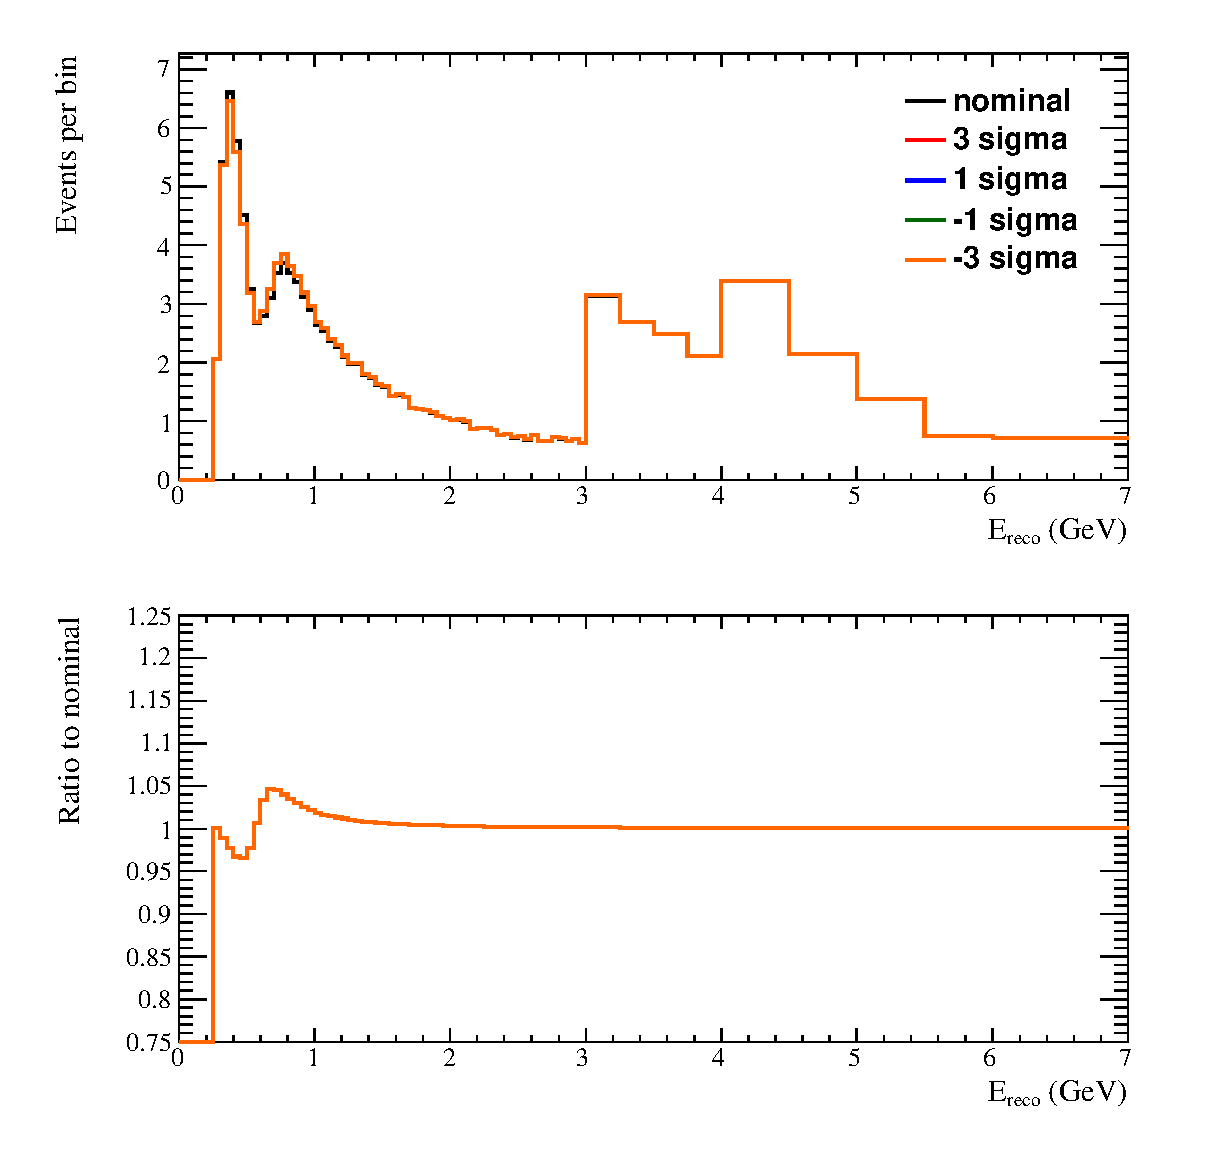
\includegraphics{../images/spectrum_tweaked/1sigma_oscillated/ereco_twk_delta_cp}}
\caption
{ Effect of $\delta_{CP}$ for 3 flavour oscillations, using oscillation parameters:  $\sin^2\theta_{12} = $0.306; $\sin^2\theta_{13} = $0.0251; $\sin^2\theta_{23} = $0.5; $\delta_{CP} = $        0; $\Delta m^2_{21} = $    7.5e-05 eV$^2$/c$^4$; $|\Delta m^2_{32}| = $    0.0024 eV$^2$/c$^4$. }
\label{fig:osc_ereco_twk_delta_cp}
\end{center}
\end{figure}
\clearpage

\begin{figure}
\begin{center}
\resizebox{14cm}{!}{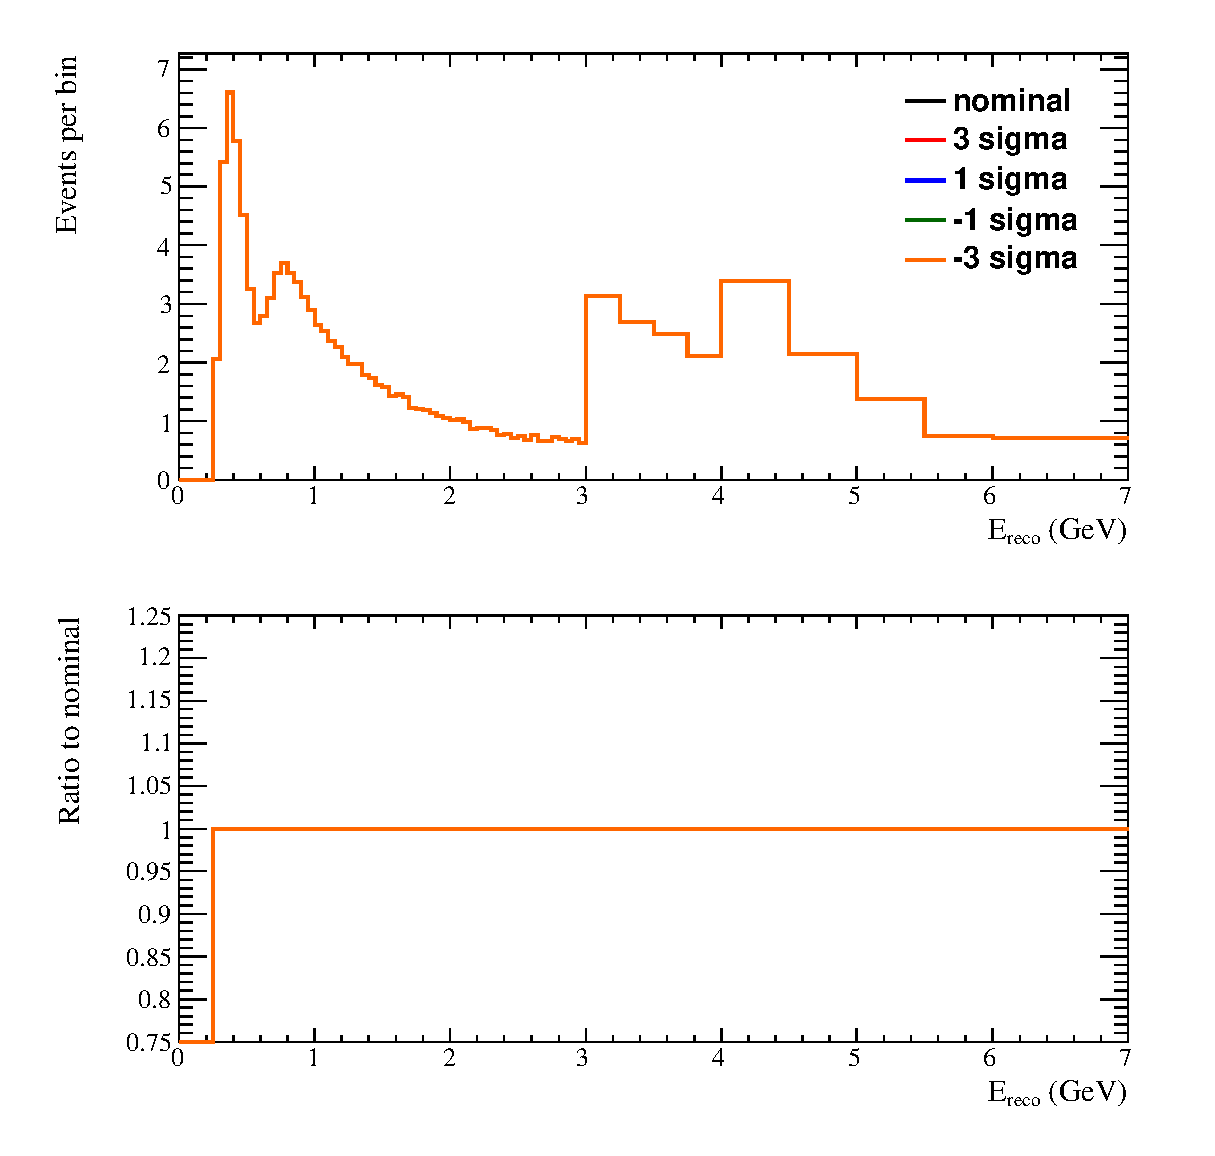
\includegraphics{../images/spectrum_tweaked/1sigma_oscillated/ereco_twk_dm12sq}}
\caption
{ Effect of $\Delta m^2_{21}$ for 3 flavour oscillations, using oscillation parameters:  $\sin^2\theta_{12} = $0.306; $\sin^2\theta_{13} = $0.0251; $\sin^2\theta_{23} = $0.5; $\delta_{CP} = $        0; $\Delta m^2_{21} = $    7.5e-05 eV$^2$/c$^4$; $|\Delta m^2_{32}| = $    0.0024 eV$^2$/c$^4$. }
\label{fig:osc_ereco_twk_dm12sq}
\end{center}
\end{figure}
\clearpage

\begin{figure}
\begin{center}
\resizebox{14cm}{!}{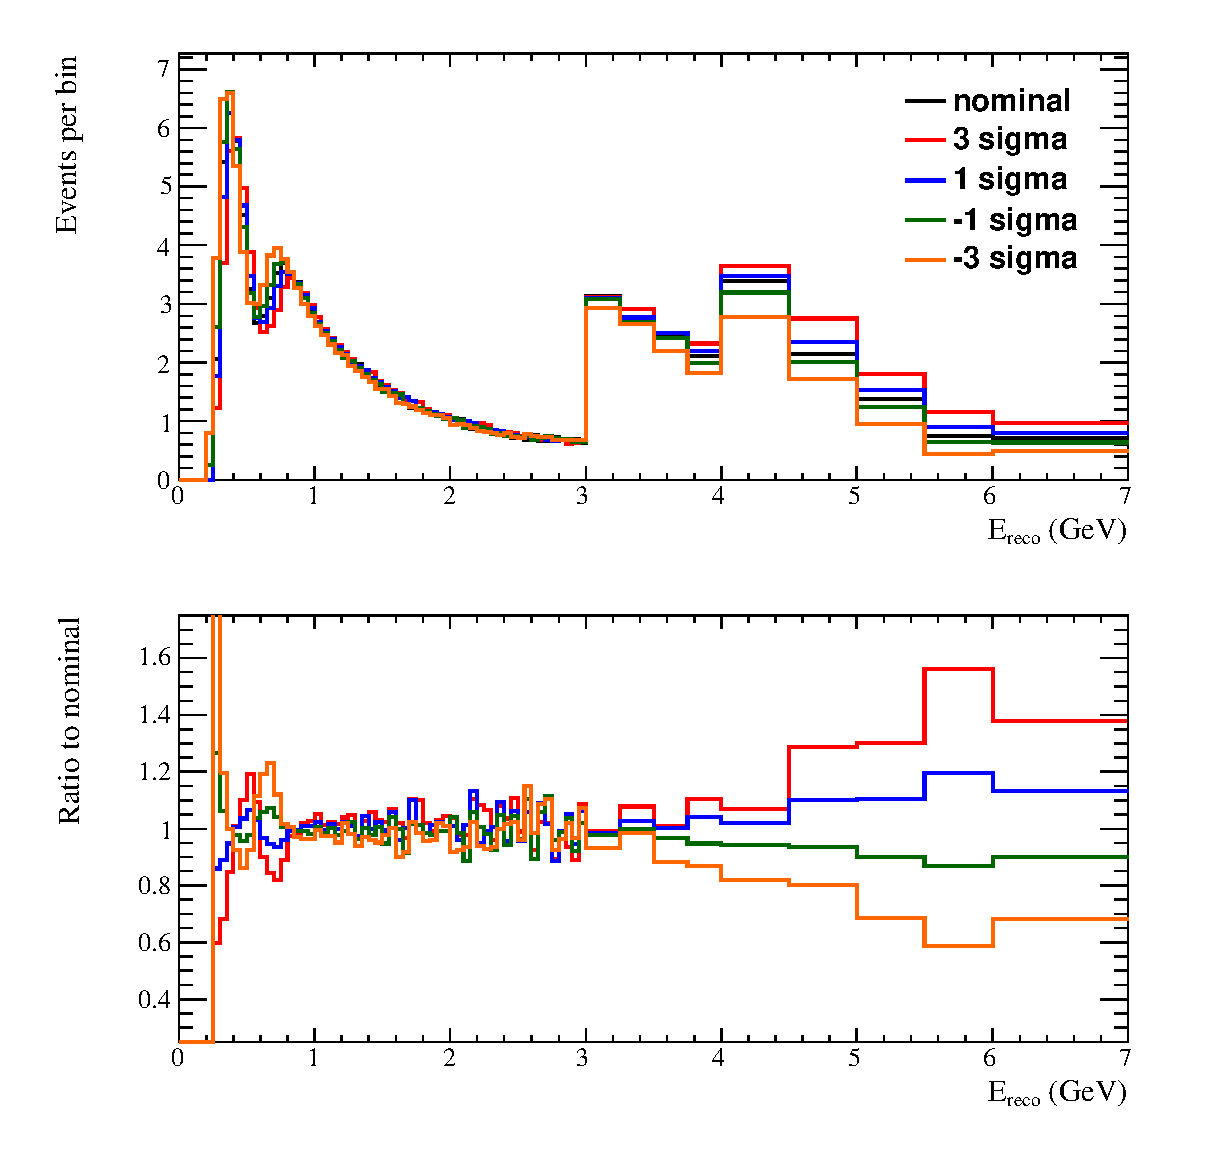
\includegraphics{../images/spectrum_tweaked/1sigma_oscillated/ereco_twk_f_sk_e_scale}}
\caption
{ Effect of $f_{E; r}^{SK}$   for 3 flavour oscillations, using oscillation parameters:  $\sin^2\theta_{12} = $0.306; $\sin^2\theta_{13} = $0.0251; $\sin^2\theta_{23} = $0.5; $\delta_{CP} = $        0; $\Delta m^2_{21} = $    7.5e-05 eV$^2$/c$^4$; $|\Delta m^2_{32}| = $    0.0024 eV$^2$/c$^4$. }
\label{fig:osc_ereco_twk_f_sk_e_scale}
\end{center}
\end{figure}
\clearpage

\begin{figure}
\begin{center}
\resizebox{14cm}{!}{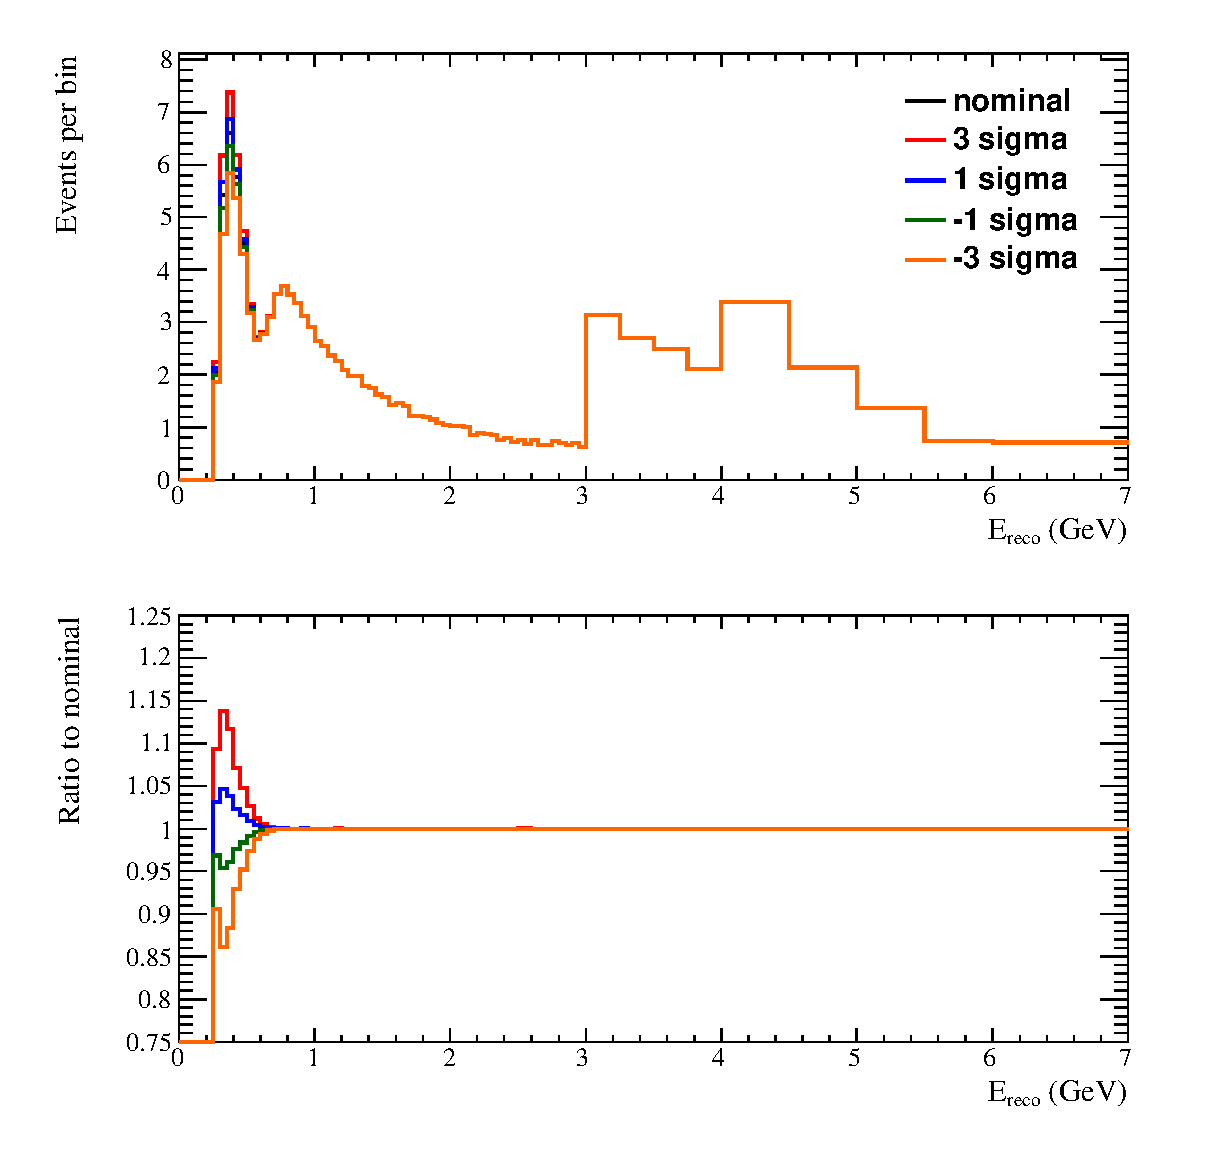
\includegraphics{../images/spectrum_tweaked/1sigma_oscillated/ereco_twk_f_banff00}}
\caption
{ Effect of $f_{0; t, r}^{banff}$ for 3 flavour oscillations, using oscillation parameters:  $\sin^2\theta_{12} = $0.306; $\sin^2\theta_{13} = $0.0251; $\sin^2\theta_{23} = $0.5; $\delta_{CP} = $        0; $\Delta m^2_{21} = $    7.5e-05 eV$^2$/c$^4$; $|\Delta m^2_{32}| = $    0.0024 eV$^2$/c$^4$. }
\label{fig:osc_ereco_twk_f_banff00}
\end{center}
\end{figure}
\clearpage

\begin{figure}
\begin{center}
\resizebox{14cm}{!}{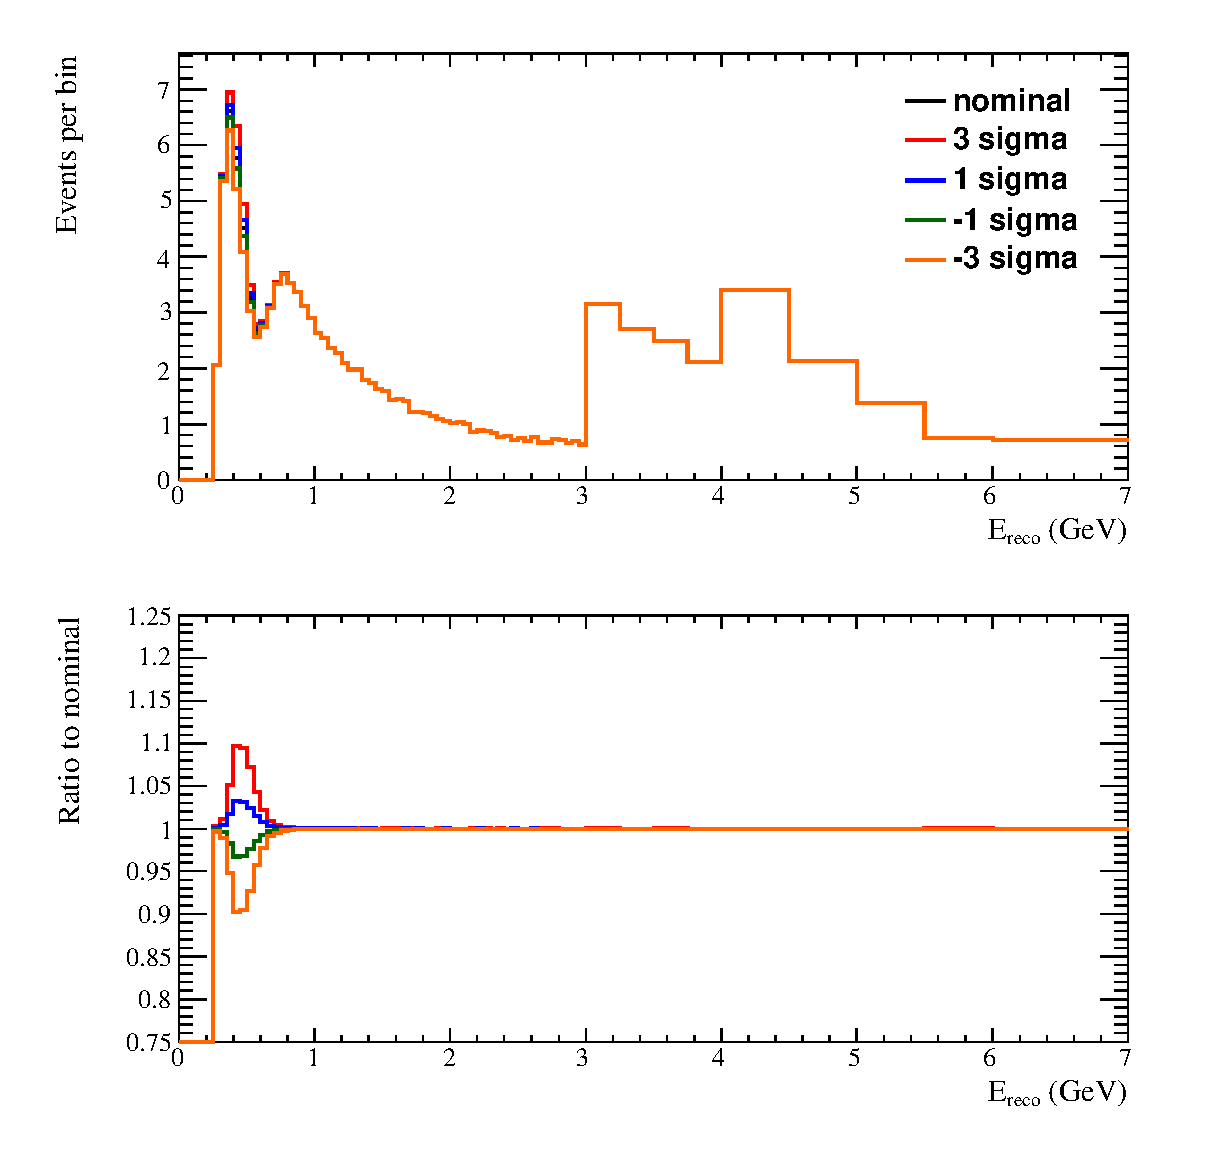
\includegraphics{../images/spectrum_tweaked/1sigma_oscillated/ereco_twk_f_banff01}}
\caption
{ Effect of $f_{1; t, r}^{banff}$ for 3 flavour oscillations, using oscillation parameters:  $\sin^2\theta_{12} = $0.306; $\sin^2\theta_{13} = $0.0251; $\sin^2\theta_{23} = $0.5; $\delta_{CP} = $        0; $\Delta m^2_{21} = $    7.5e-05 eV$^2$/c$^4$; $|\Delta m^2_{32}| = $    0.0024 eV$^2$/c$^4$. }
\label{fig:osc_ereco_twk_f_banff01}
\end{center}
\end{figure}
\clearpage

\begin{figure}
\begin{center}
\resizebox{14cm}{!}{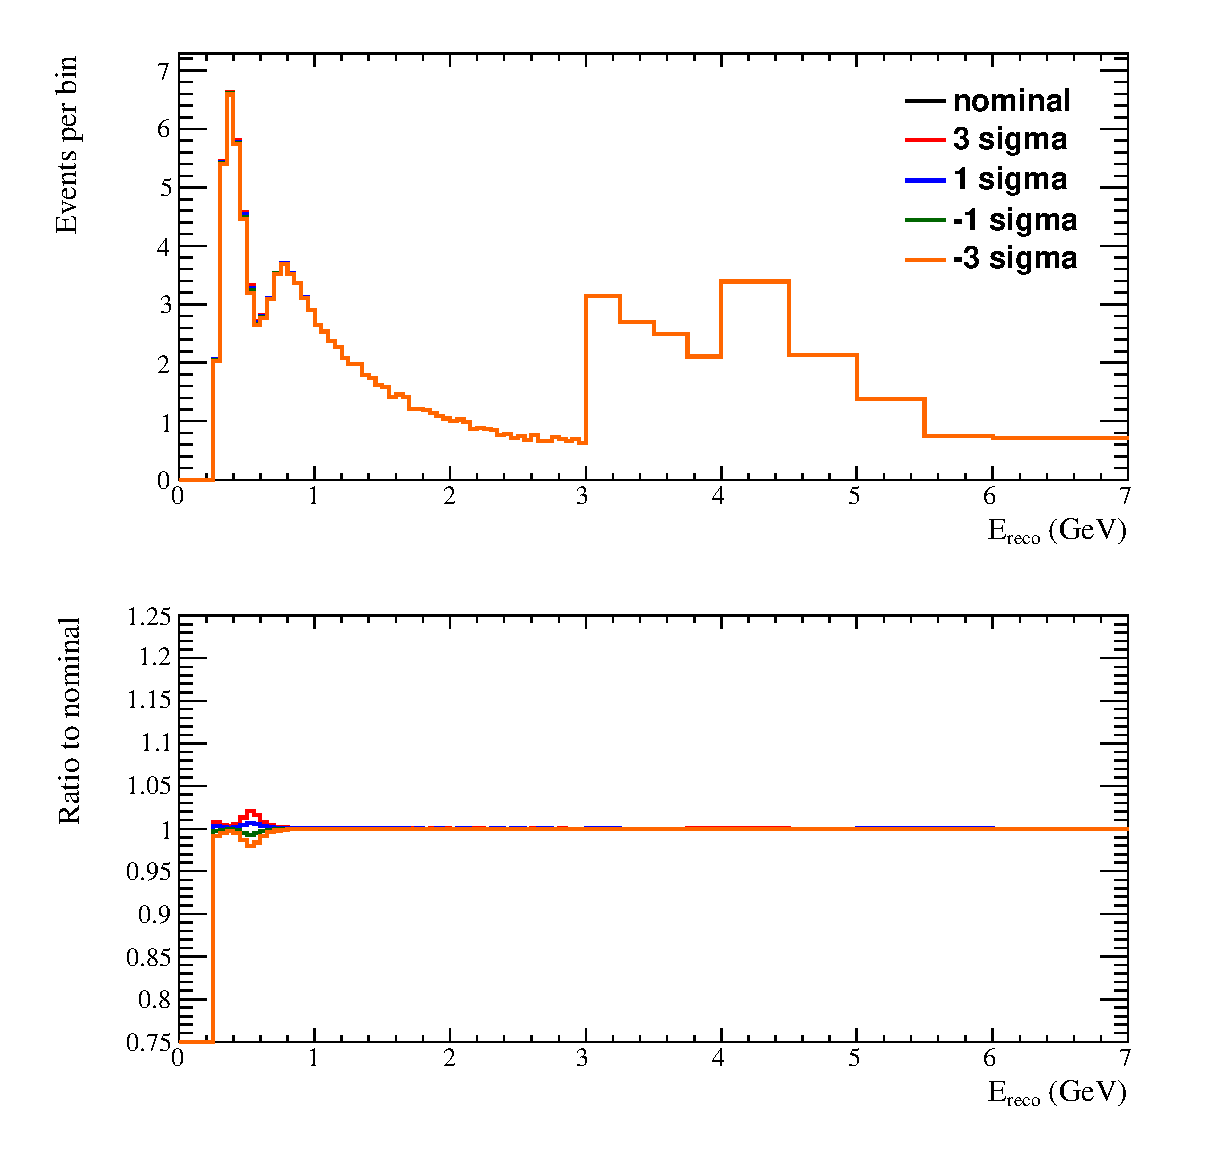
\includegraphics{../images/spectrum_tweaked/1sigma_oscillated/ereco_twk_f_banff02}}
\caption
{ Effect of $f_{2; t, r}^{banff}$ for 3 flavour oscillations, using oscillation parameters:  $\sin^2\theta_{12} = $0.306; $\sin^2\theta_{13} = $0.0251; $\sin^2\theta_{23} = $0.5; $\delta_{CP} = $        0; $\Delta m^2_{21} = $    7.5e-05 eV$^2$/c$^4$; $|\Delta m^2_{32}| = $    0.0024 eV$^2$/c$^4$. }
\label{fig:osc_ereco_twk_f_banff02}
\end{center}
\end{figure}
\clearpage

\begin{figure}
\begin{center}
\resizebox{14cm}{!}{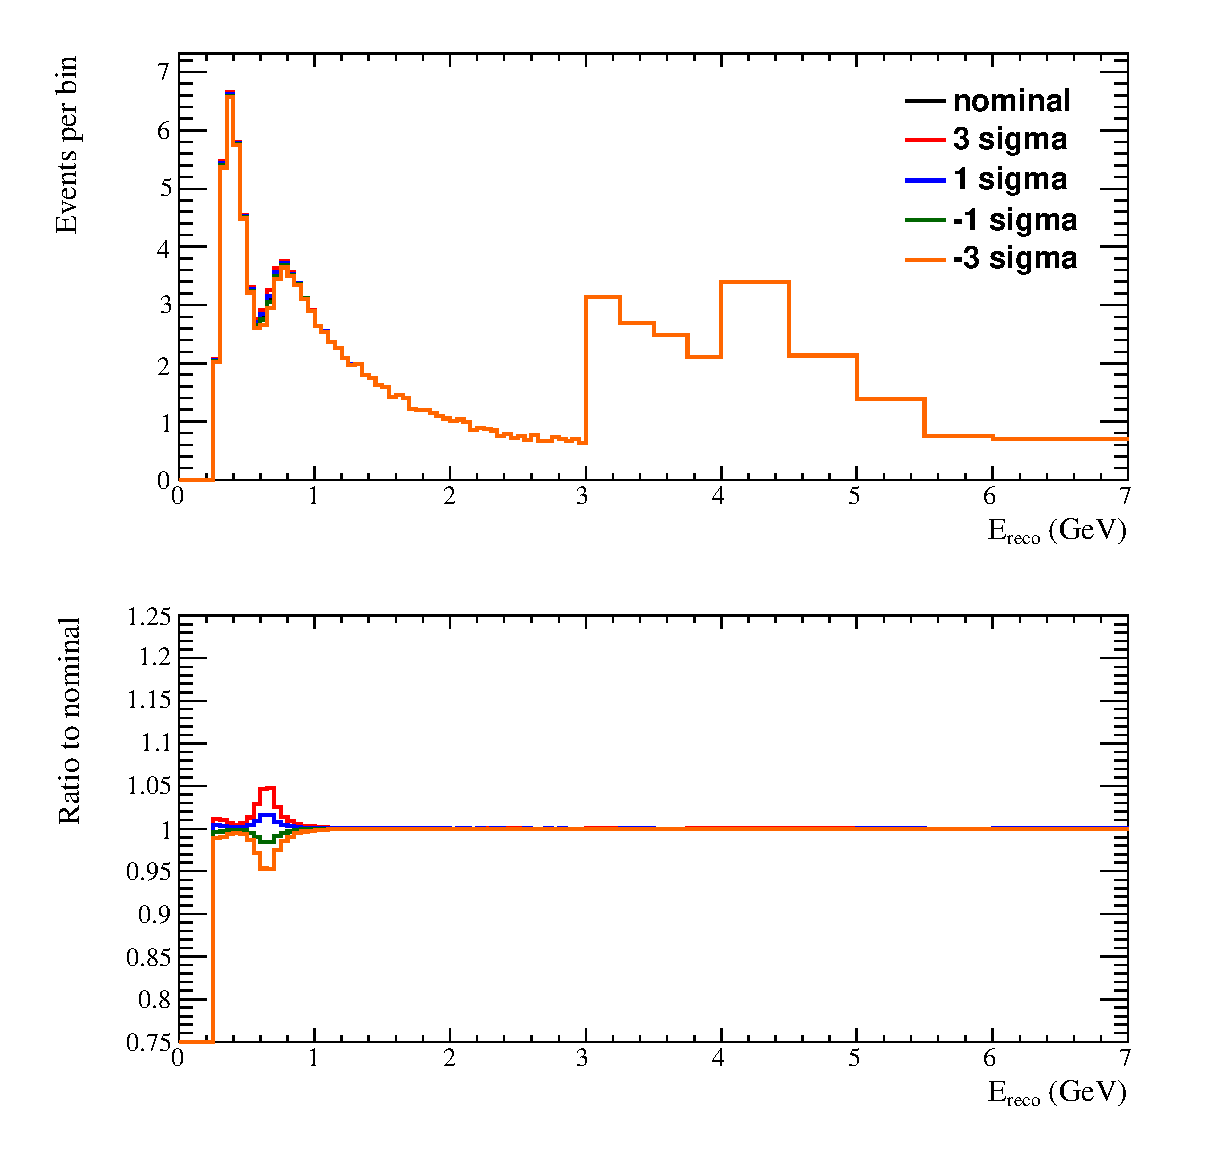
\includegraphics{../images/spectrum_tweaked/1sigma_oscillated/ereco_twk_f_banff03}}
\caption
{ Effect of $f_{3; t, r}^{banff}$ for 3 flavour oscillations, using oscillation parameters:  $\sin^2\theta_{12} = $0.306; $\sin^2\theta_{13} = $0.0251; $\sin^2\theta_{23} = $0.5; $\delta_{CP} = $        0; $\Delta m^2_{21} = $    7.5e-05 eV$^2$/c$^4$; $|\Delta m^2_{32}| = $    0.0024 eV$^2$/c$^4$. }
\label{fig:osc_ereco_twk_f_banff03}
\end{center}
\end{figure}
\clearpage

\begin{figure}
\begin{center}
\resizebox{14cm}{!}{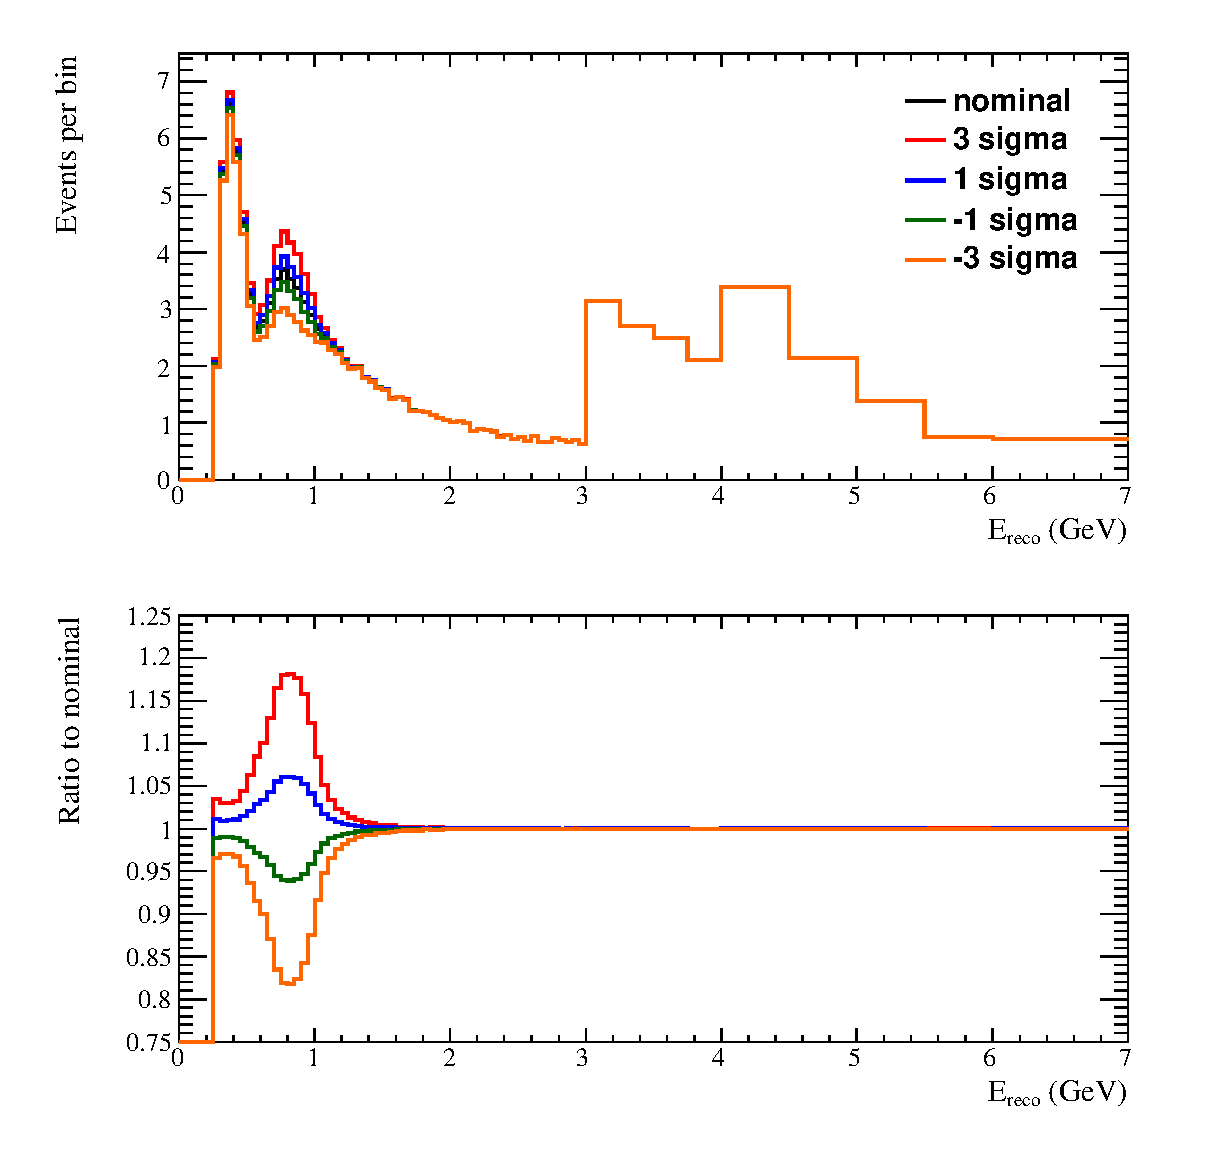
\includegraphics{../images/spectrum_tweaked/1sigma_oscillated/ereco_twk_f_banff04}}
\caption
{ Effect of $f_{4; t, r}^{banff}$ for 3 flavour oscillations, using oscillation parameters:  $\sin^2\theta_{12} = $0.306; $\sin^2\theta_{13} = $0.0251; $\sin^2\theta_{23} = $0.5; $\delta_{CP} = $        0; $\Delta m^2_{21} = $    7.5e-05 eV$^2$/c$^4$; $|\Delta m^2_{32}| = $    0.0024 eV$^2$/c$^4$. }
\label{fig:osc_ereco_twk_f_banff04}
\end{center}
\end{figure}
\clearpage

\begin{figure}
\begin{center}
\resizebox{14cm}{!}{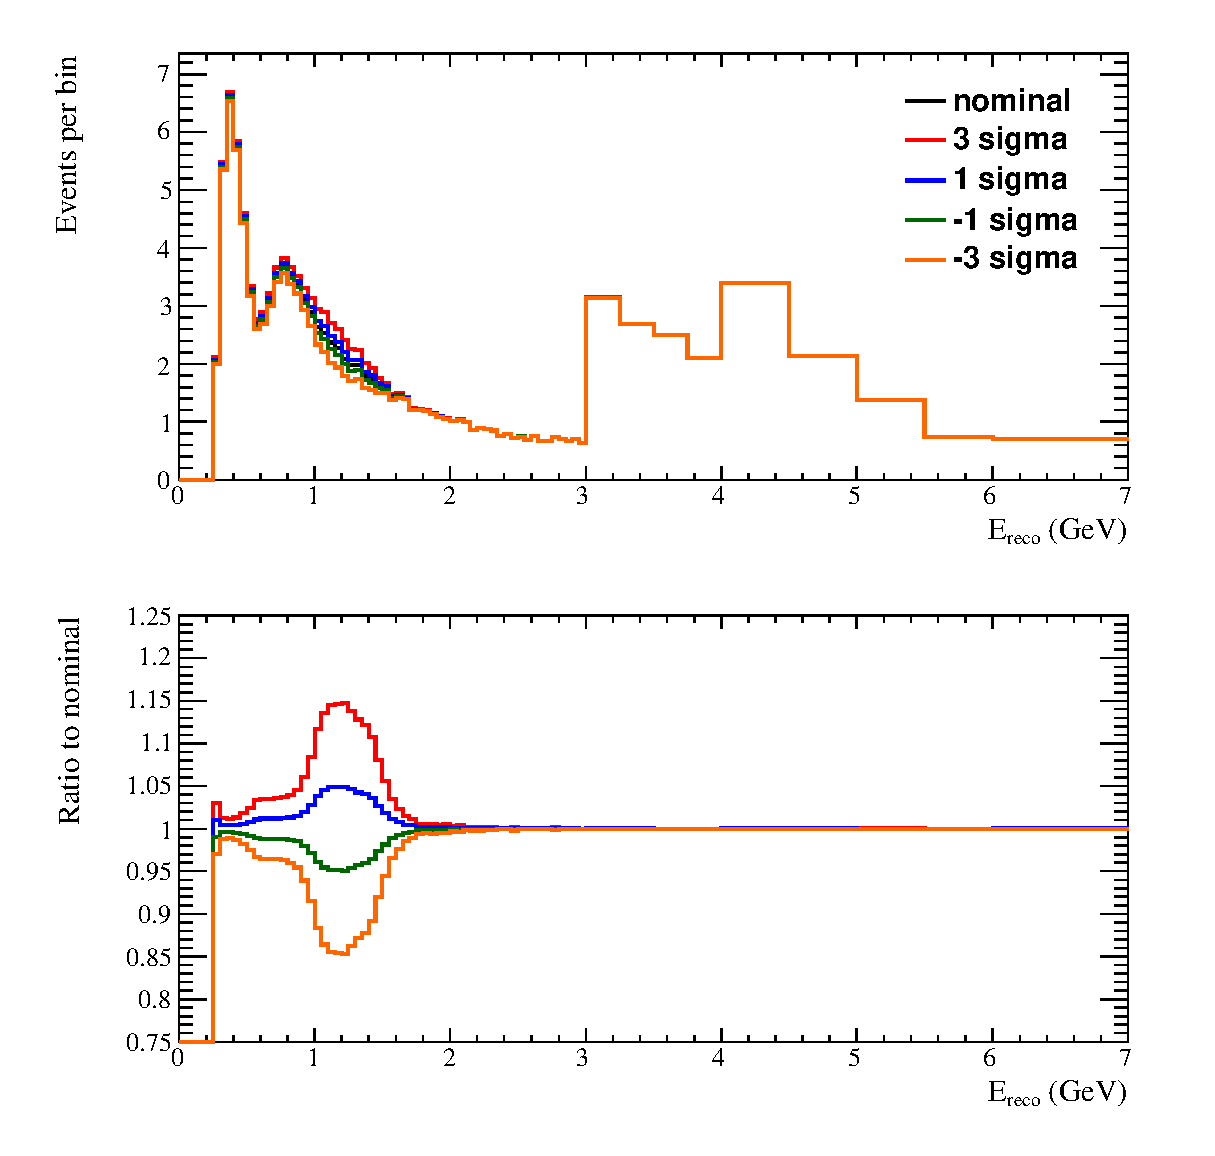
\includegraphics{../images/spectrum_tweaked/1sigma_oscillated/ereco_twk_f_banff05}}
\caption
{ Effect of $f_{5; t, r}^{banff}$ for 3 flavour oscillations, using oscillation parameters:  $\sin^2\theta_{12} = $0.306; $\sin^2\theta_{13} = $0.0251; $\sin^2\theta_{23} = $0.5; $\delta_{CP} = $        0; $\Delta m^2_{21} = $    7.5e-05 eV$^2$/c$^4$; $|\Delta m^2_{32}| = $    0.0024 eV$^2$/c$^4$. }
\label{fig:osc_ereco_twk_f_banff05}
\end{center}
\end{figure}
\clearpage

\begin{figure}
\begin{center}
\resizebox{14cm}{!}{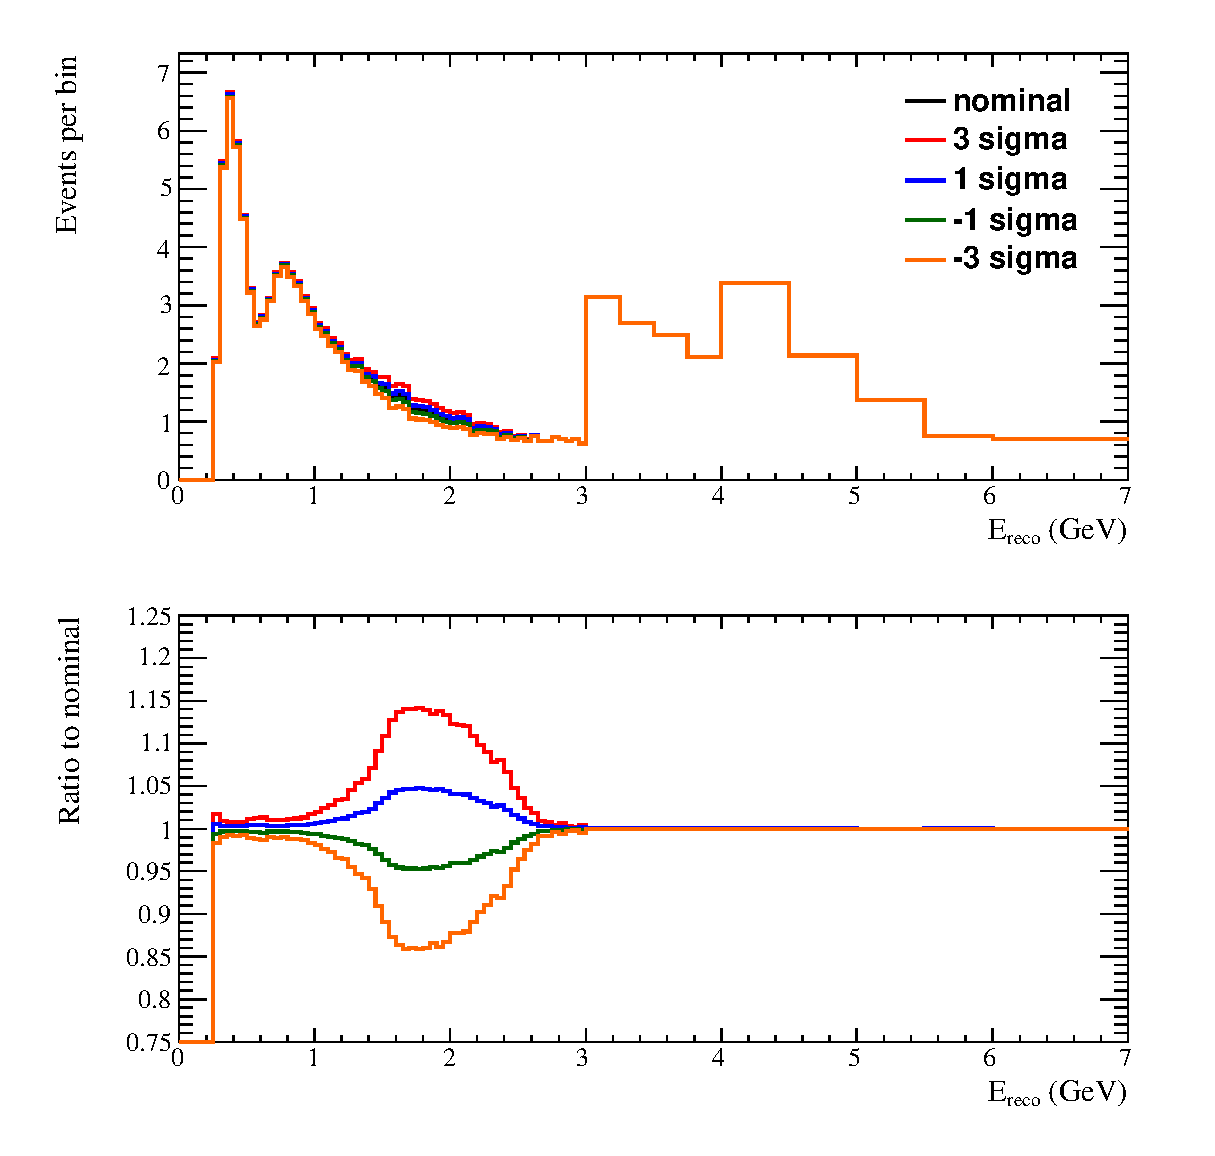
\includegraphics{../images/spectrum_tweaked/1sigma_oscillated/ereco_twk_f_banff06}}
\caption
{ Effect of $f_{6; t, r}^{banff}$ for 3 flavour oscillations, using oscillation parameters:  $\sin^2\theta_{12} = $0.306; $\sin^2\theta_{13} = $0.0251; $\sin^2\theta_{23} = $0.5; $\delta_{CP} = $        0; $\Delta m^2_{21} = $    7.5e-05 eV$^2$/c$^4$; $|\Delta m^2_{32}| = $    0.0024 eV$^2$/c$^4$. }
\label{fig:osc_ereco_twk_f_banff06}
\end{center}
\end{figure}
\clearpage

\begin{figure}
\begin{center}
\resizebox{14cm}{!}{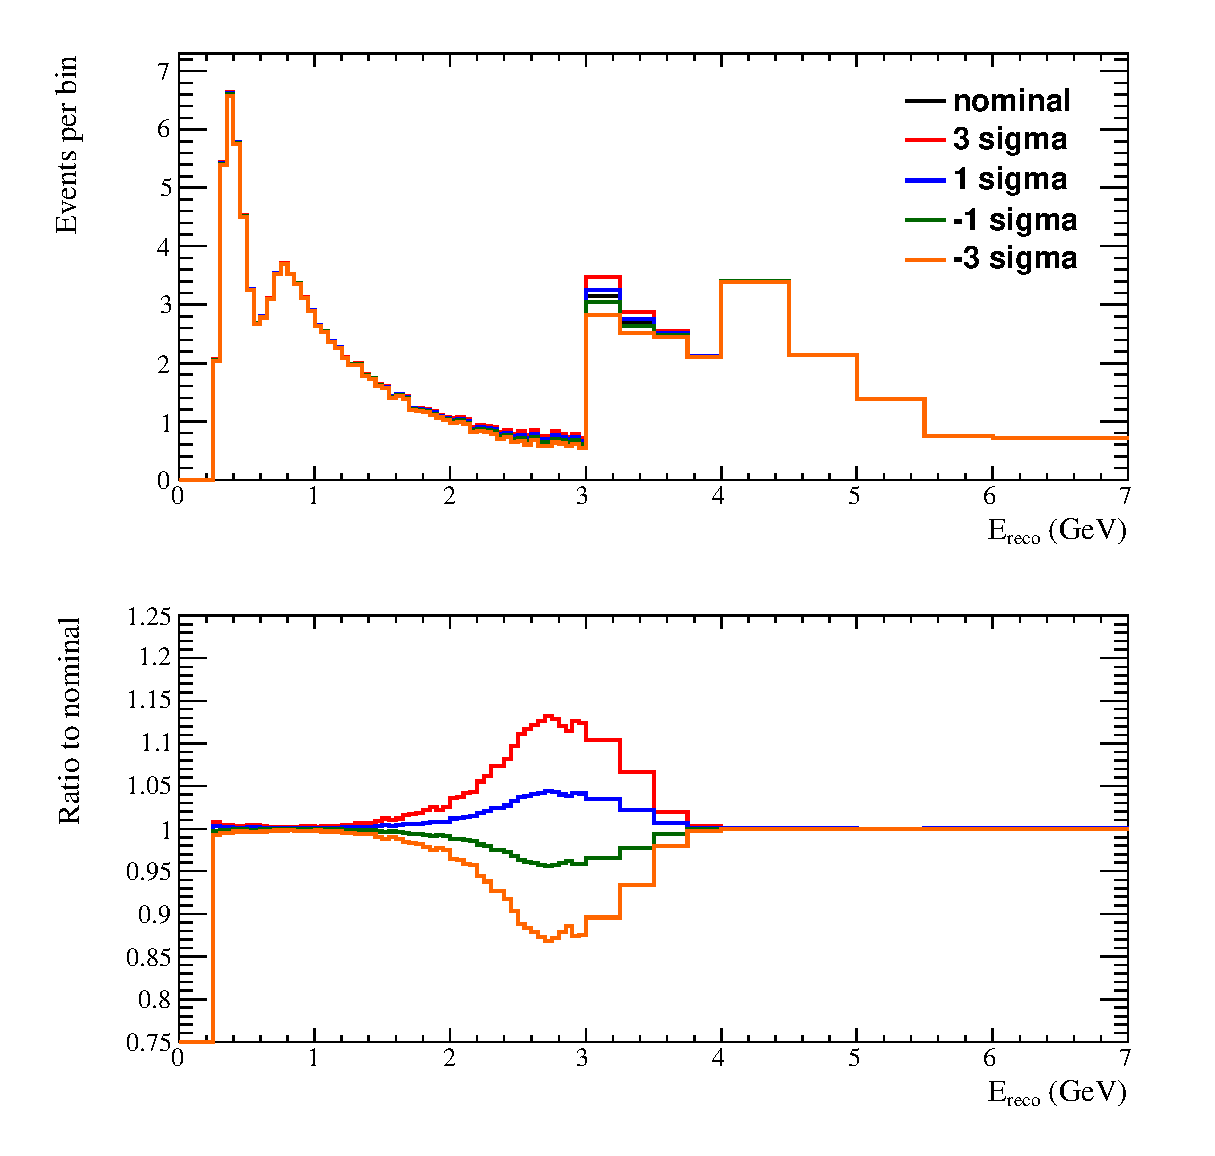
\includegraphics{../images/spectrum_tweaked/1sigma_oscillated/ereco_twk_f_banff07}}
\caption
{ Effect of $f_{7; t, r}^{banff}$ for 3 flavour oscillations, using oscillation parameters:  $\sin^2\theta_{12} = $0.306; $\sin^2\theta_{13} = $0.0251; $\sin^2\theta_{23} = $0.5; $\delta_{CP} = $        0; $\Delta m^2_{21} = $    7.5e-05 eV$^2$/c$^4$; $|\Delta m^2_{32}| = $    0.0024 eV$^2$/c$^4$. }
\label{fig:osc_ereco_twk_f_banff07}
\end{center}
\end{figure}
\clearpage

\begin{figure}
\begin{center}
\resizebox{14cm}{!}{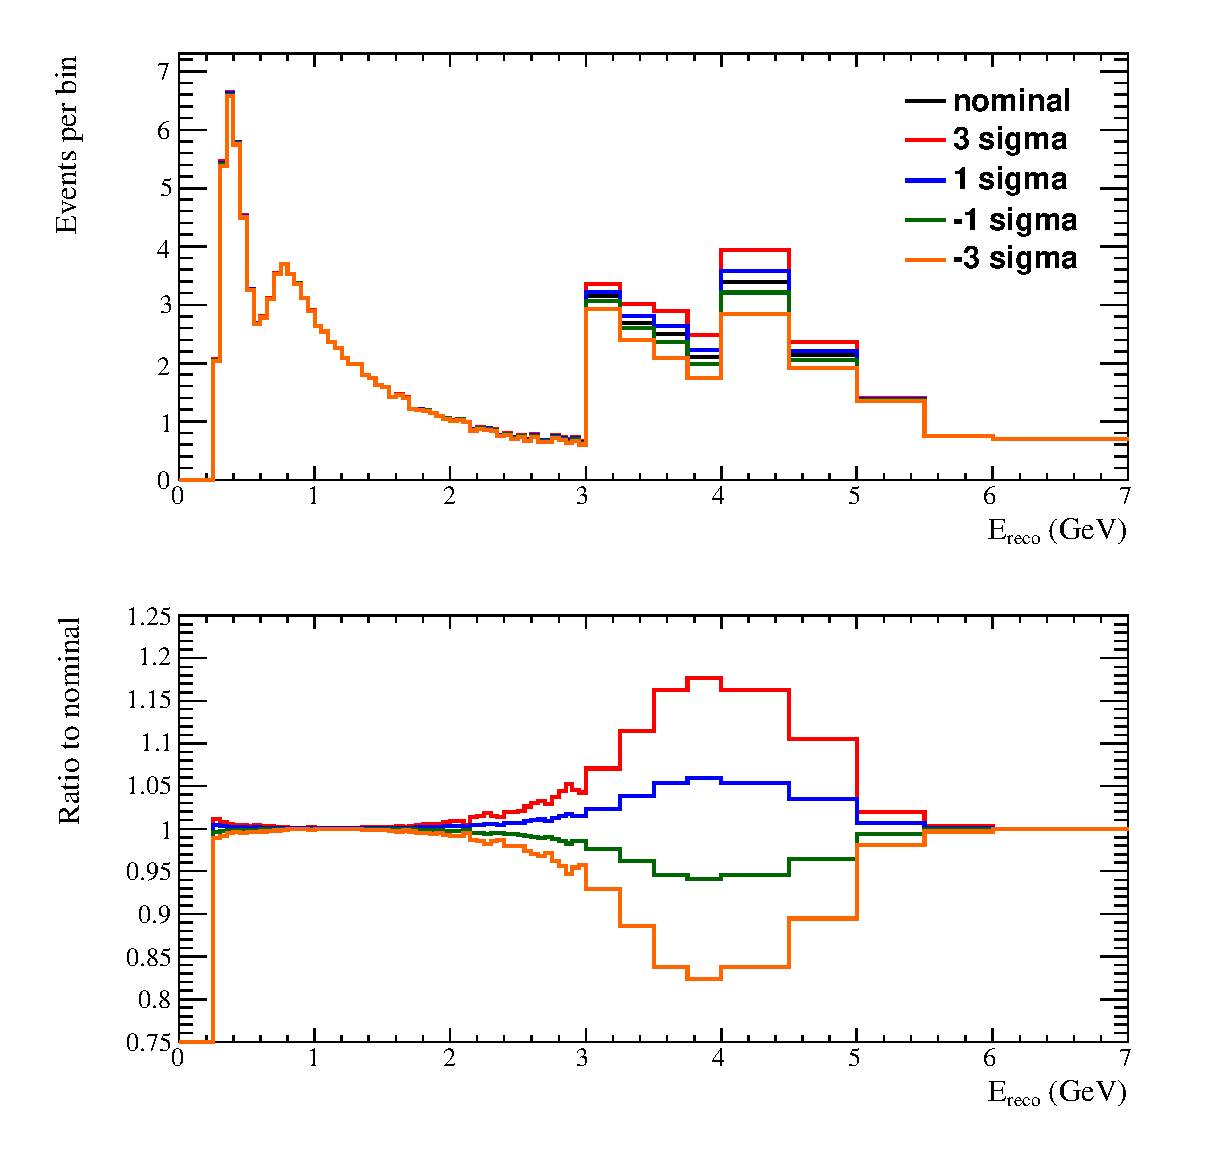
\includegraphics{../images/spectrum_tweaked/1sigma_oscillated/ereco_twk_f_banff08}}
\caption
{ Effect of $f_{8; t, r}^{banff}$ for 3 flavour oscillations, using oscillation parameters:  $\sin^2\theta_{12} = $0.306; $\sin^2\theta_{13} = $0.0251; $\sin^2\theta_{23} = $0.5; $\delta_{CP} = $        0; $\Delta m^2_{21} = $    7.5e-05 eV$^2$/c$^4$; $|\Delta m^2_{32}| = $    0.0024 eV$^2$/c$^4$. }
\label{fig:osc_ereco_twk_f_banff08}
\end{center}
\end{figure}
\clearpage

\begin{figure}
\begin{center}
\resizebox{14cm}{!}{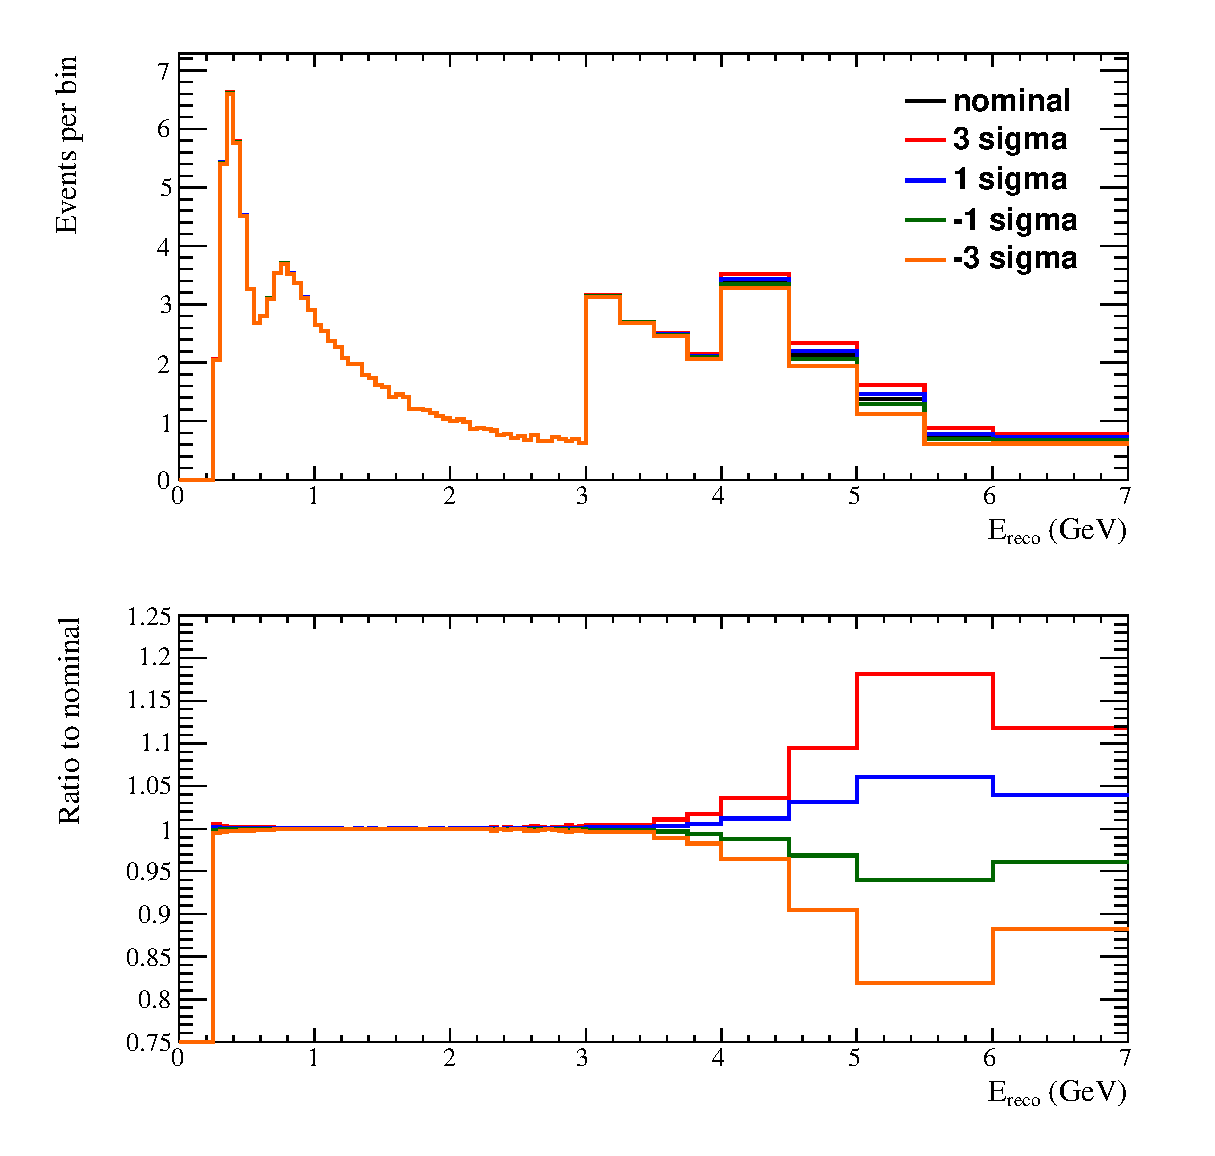
\includegraphics{../images/spectrum_tweaked/1sigma_oscillated/ereco_twk_f_banff09}}
\caption
{ Effect of $f_{9; t, r}^{banff}$ for 3 flavour oscillations, using oscillation parameters:  $\sin^2\theta_{12} = $0.306; $\sin^2\theta_{13} = $0.0251; $\sin^2\theta_{23} = $0.5; $\delta_{CP} = $        0; $\Delta m^2_{21} = $    7.5e-05 eV$^2$/c$^4$; $|\Delta m^2_{32}| = $    0.0024 eV$^2$/c$^4$. }
\label{fig:osc_ereco_twk_f_banff09}
\end{center}
\end{figure}
\clearpage

\begin{figure}
\begin{center}
\resizebox{14cm}{!}{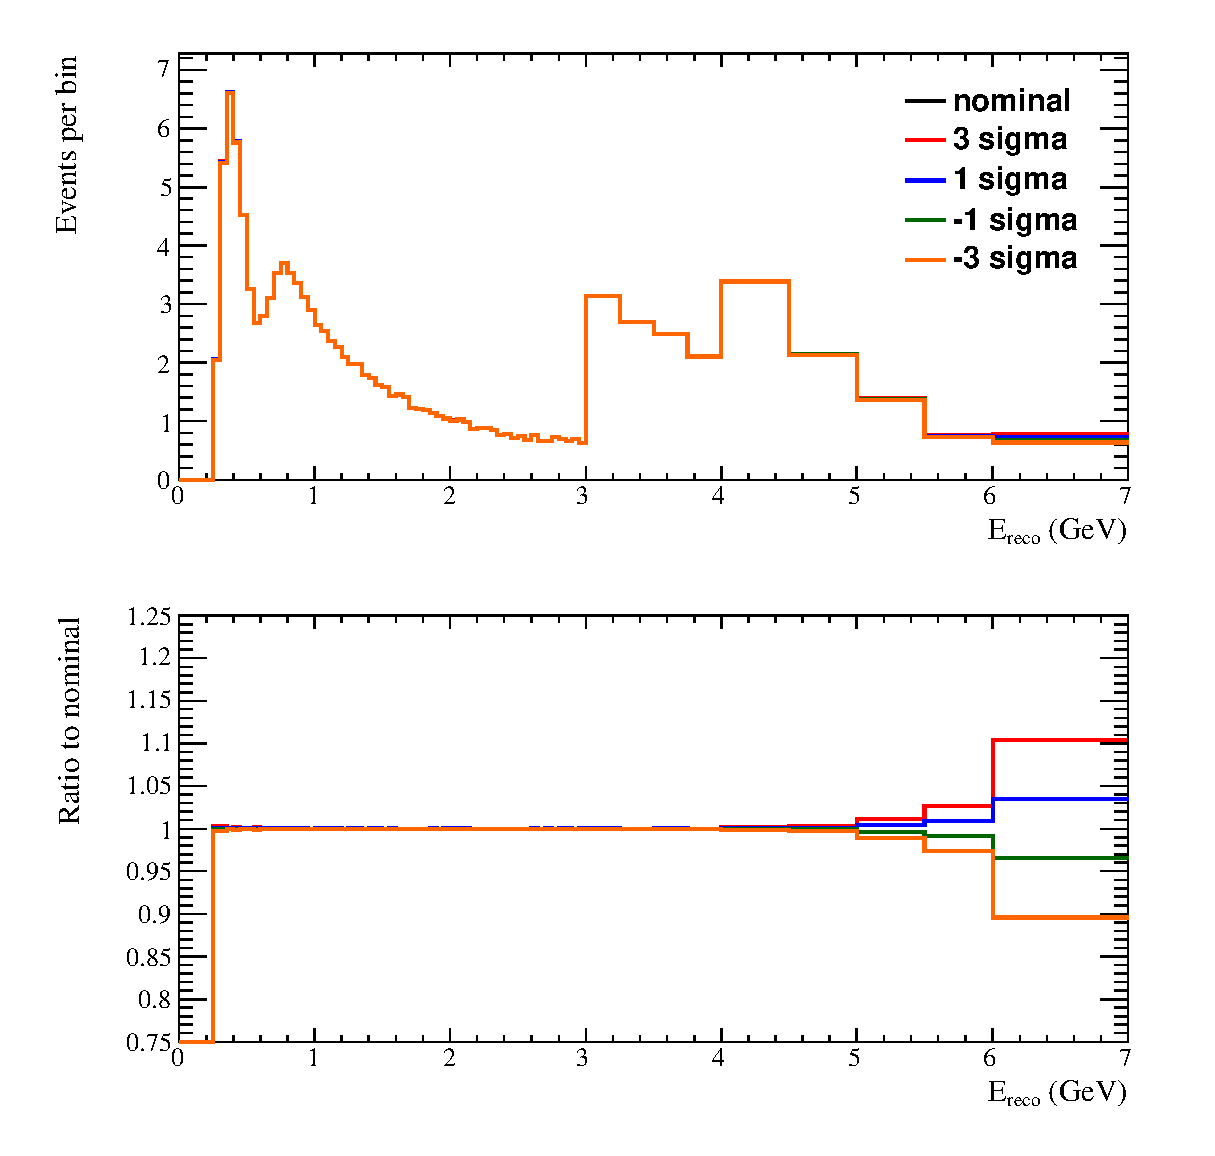
\includegraphics{../images/spectrum_tweaked/1sigma_oscillated/ereco_twk_f_banff10}}
\caption
{ Effect of $f_{10; t, r}^{banff}$ for 3 flavour oscillations, using oscillation parameters:  $\sin^2\theta_{12} = $0.306; $\sin^2\theta_{13} = $0.0251; $\sin^2\theta_{23} = $0.5; $\delta_{CP} = $        0; $\Delta m^2_{21} = $    7.5e-05 eV$^2$/c$^4$; $|\Delta m^2_{32}| = $    0.0024 eV$^2$/c$^4$. }
\label{fig:osc_ereco_twk_f_banff10}
\end{center}
\end{figure}
\clearpage

\begin{figure}
\begin{center}
\resizebox{14cm}{!}{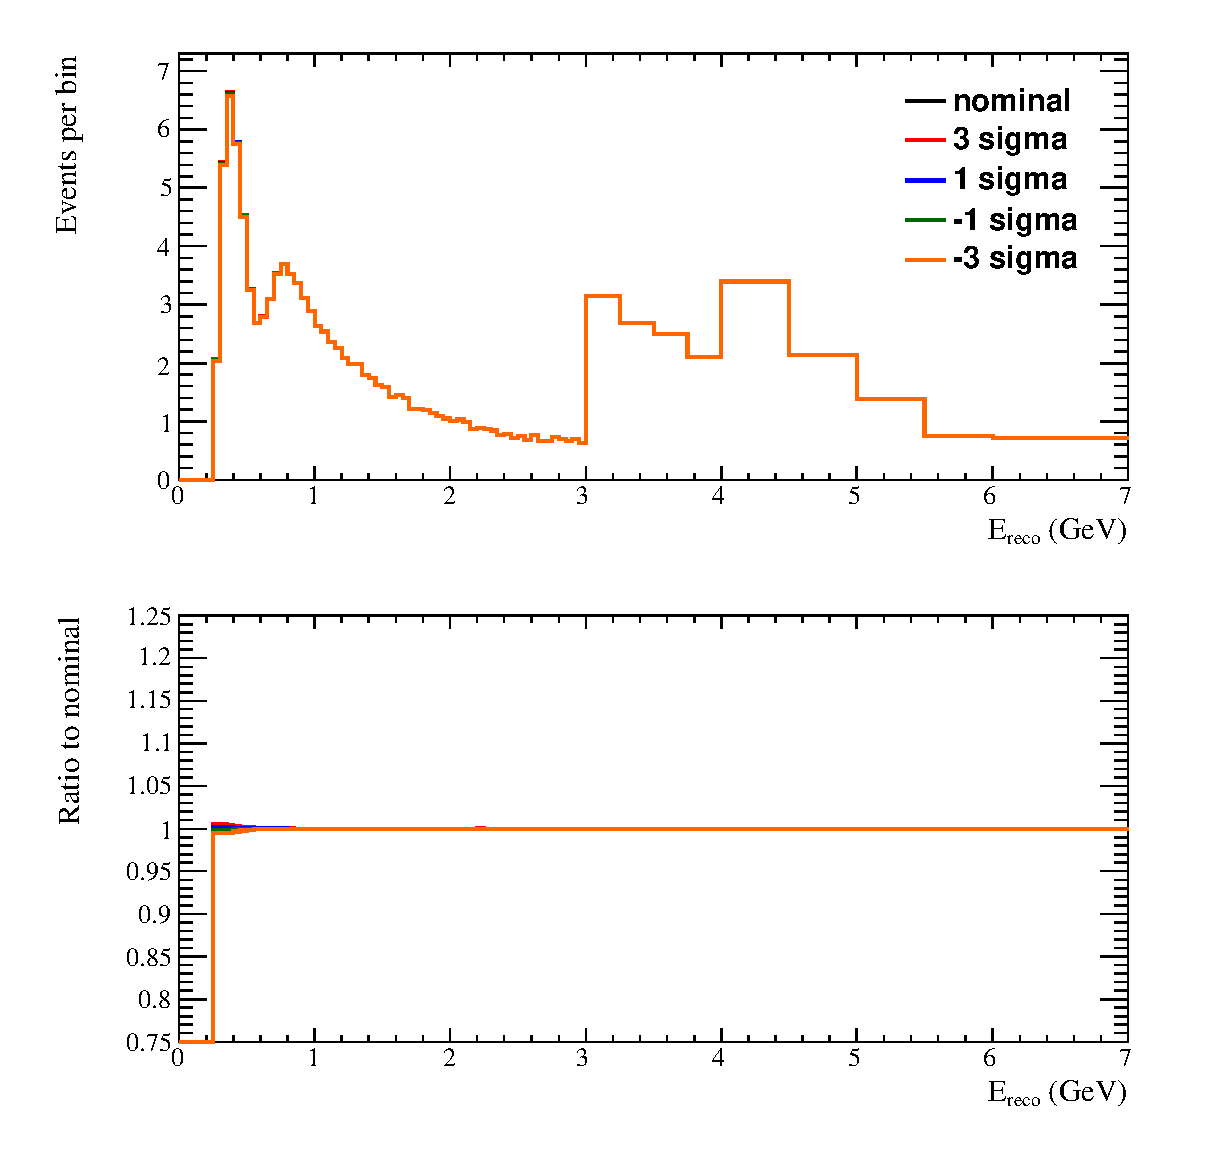
\includegraphics{../images/spectrum_tweaked/1sigma_oscillated/ereco_twk_f_banff11}}
\caption
{ Effect of $f_{11; t, r}^{banff}$ for 3 flavour oscillations, using oscillation parameters:  $\sin^2\theta_{12} = $0.306; $\sin^2\theta_{13} = $0.0251; $\sin^2\theta_{23} = $0.5; $\delta_{CP} = $        0; $\Delta m^2_{21} = $    7.5e-05 eV$^2$/c$^4$; $|\Delta m^2_{32}| = $    0.0024 eV$^2$/c$^4$. }
\label{fig:osc_ereco_twk_f_banff11}
\end{center}
\end{figure}
\clearpage

\begin{figure}
\begin{center}
\resizebox{14cm}{!}{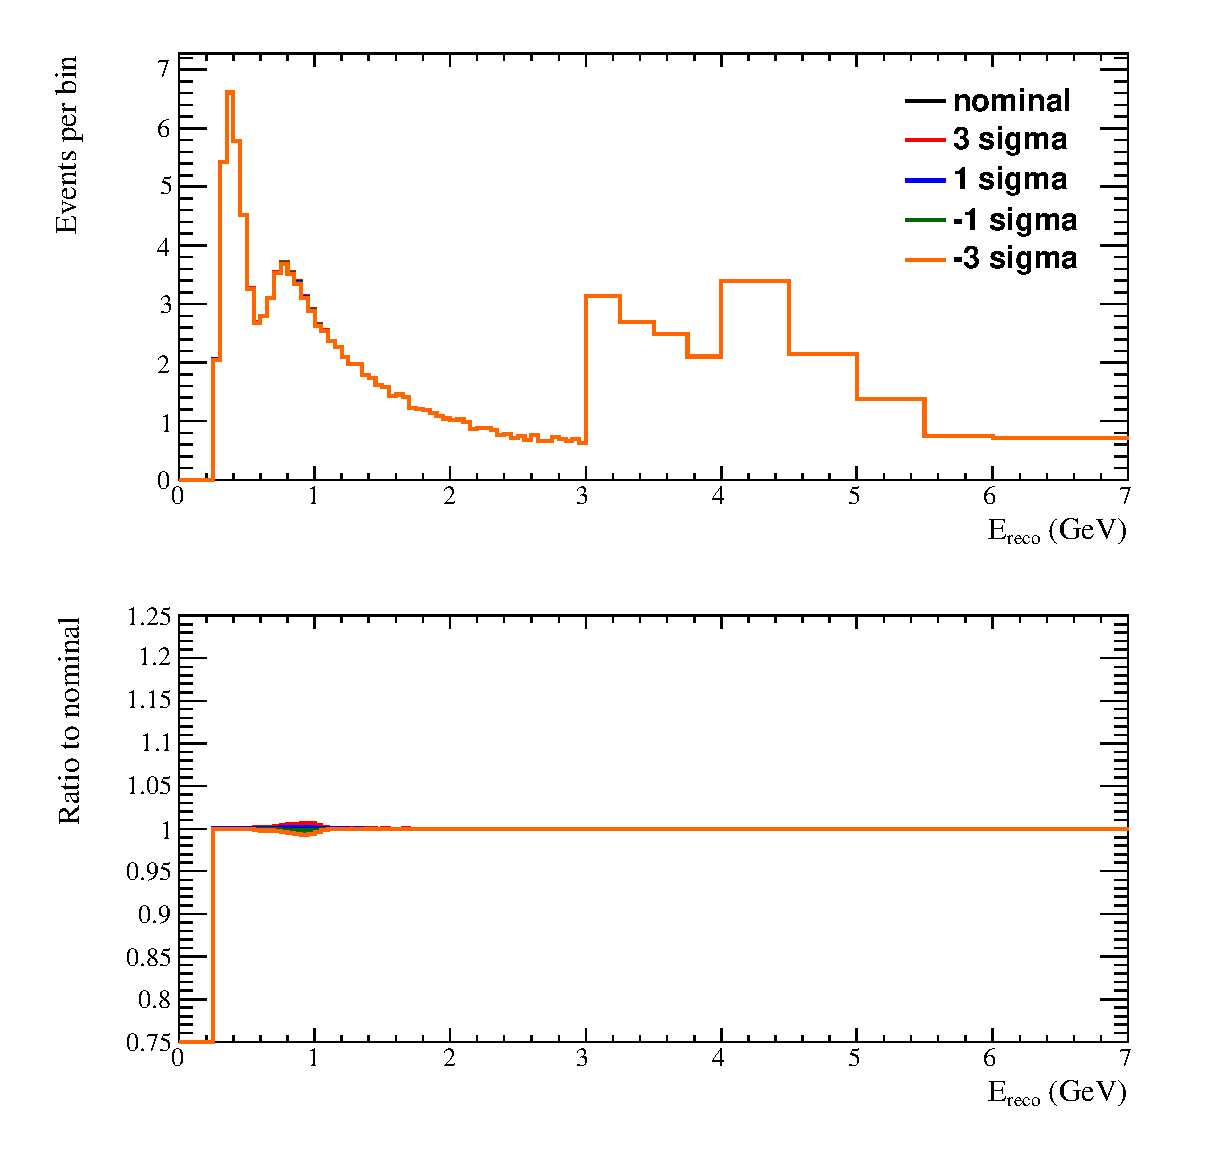
\includegraphics{../images/spectrum_tweaked/1sigma_oscillated/ereco_twk_f_banff12}}
\caption
{ Effect of $f_{12; t, r}^{banff}$ for 3 flavour oscillations, using oscillation parameters:  $\sin^2\theta_{12} = $0.306; $\sin^2\theta_{13} = $0.0251; $\sin^2\theta_{23} = $0.5; $\delta_{CP} = $        0; $\Delta m^2_{21} = $    7.5e-05 eV$^2$/c$^4$; $|\Delta m^2_{32}| = $    0.0024 eV$^2$/c$^4$. }
\label{fig:osc_ereco_twk_f_banff12}
\end{center}
\end{figure}
\clearpage

\begin{figure}
\begin{center}
\resizebox{14cm}{!}{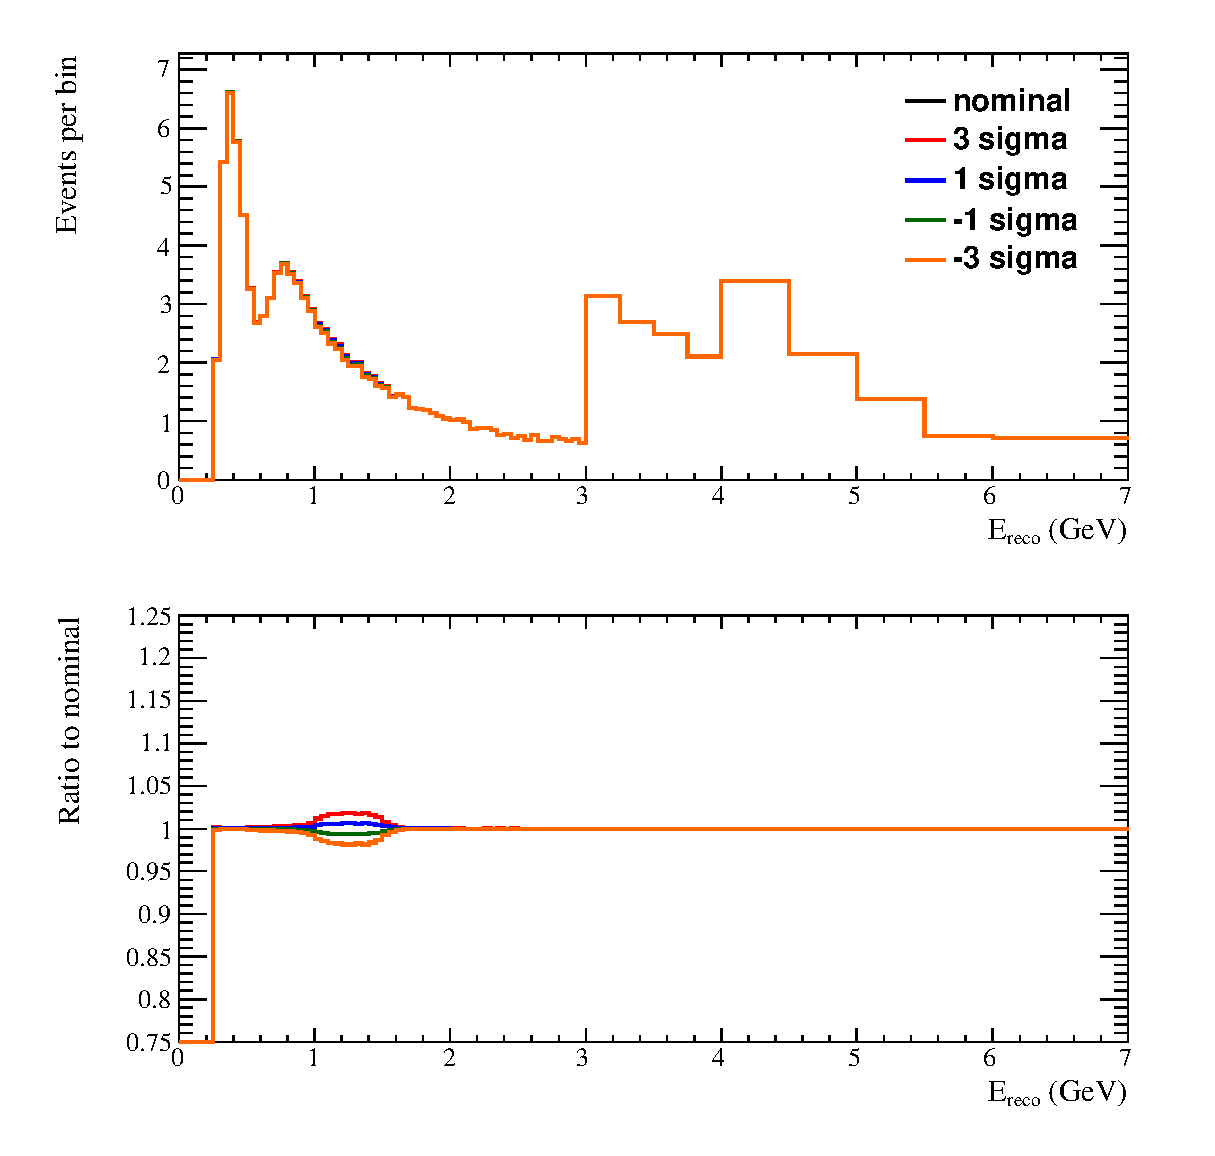
\includegraphics{../images/spectrum_tweaked/1sigma_oscillated/ereco_twk_f_banff13}}
\caption
{ Effect of $f_{13; t, r}^{banff}$ for 3 flavour oscillations, using oscillation parameters:  $\sin^2\theta_{12} = $0.306; $\sin^2\theta_{13} = $0.0251; $\sin^2\theta_{23} = $0.5; $\delta_{CP} = $        0; $\Delta m^2_{21} = $    7.5e-05 eV$^2$/c$^4$; $|\Delta m^2_{32}| = $    0.0024 eV$^2$/c$^4$. }
\label{fig:osc_ereco_twk_f_banff13}
\end{center}
\end{figure}
\clearpage

\begin{figure}
\begin{center}
\resizebox{14cm}{!}{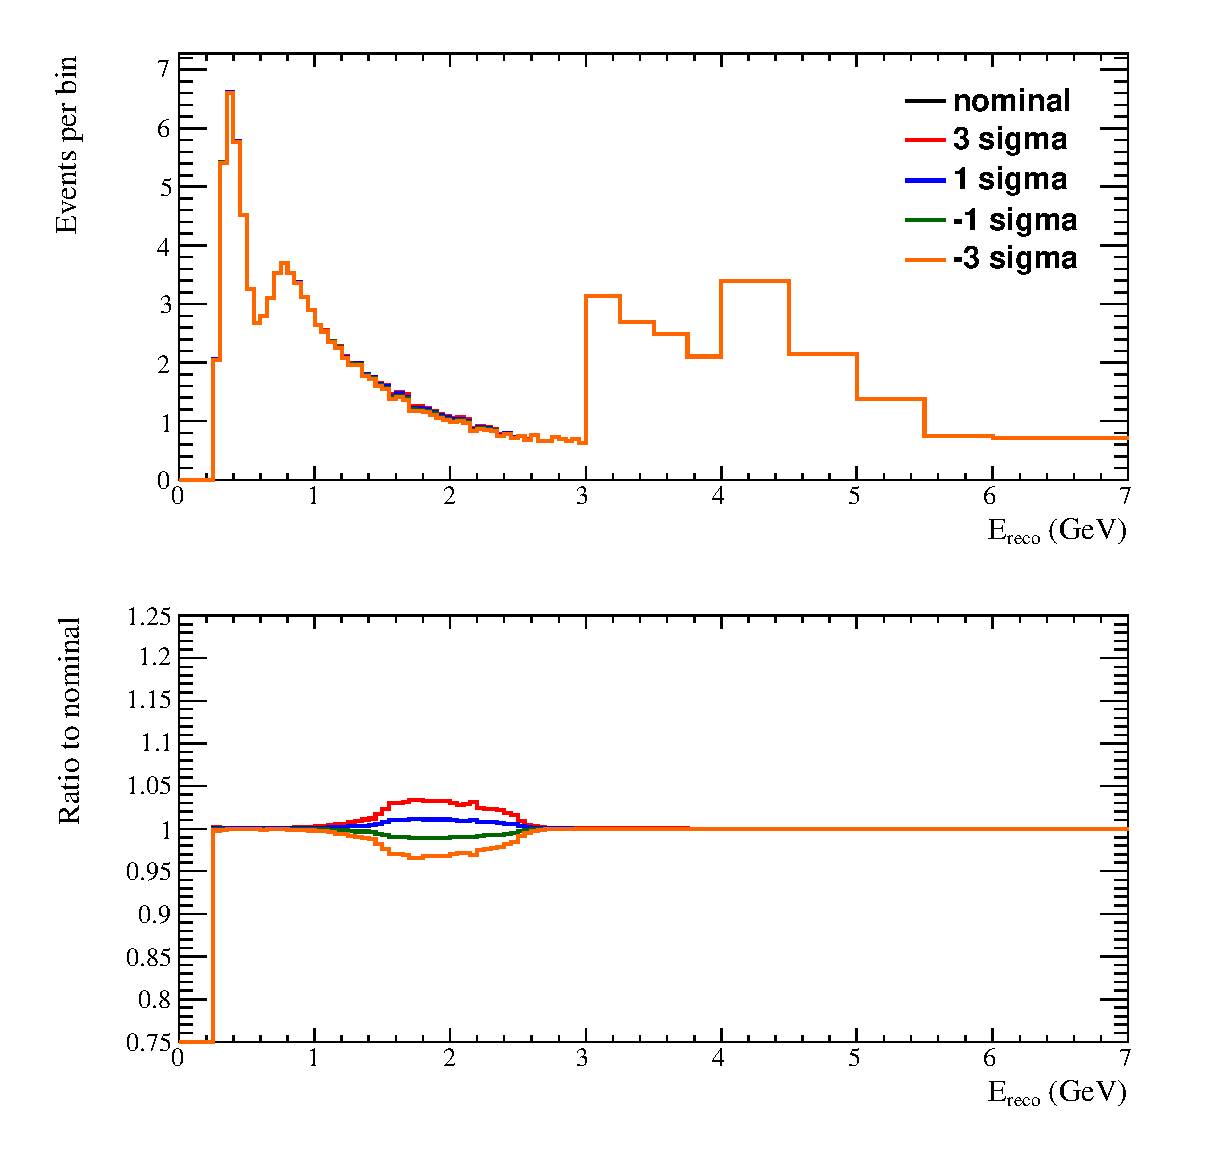
\includegraphics{../images/spectrum_tweaked/1sigma_oscillated/ereco_twk_f_banff14}}
\caption
{ Effect of $f_{14; t, r}^{banff}$ for 3 flavour oscillations, using oscillation parameters:  $\sin^2\theta_{12} = $0.306; $\sin^2\theta_{13} = $0.0251; $\sin^2\theta_{23} = $0.5; $\delta_{CP} = $        0; $\Delta m^2_{21} = $    7.5e-05 eV$^2$/c$^4$; $|\Delta m^2_{32}| = $    0.0024 eV$^2$/c$^4$. }
\label{fig:osc_ereco_twk_f_banff14}
\end{center}
\end{figure}
\clearpage

\begin{figure}
\begin{center}
\resizebox{14cm}{!}{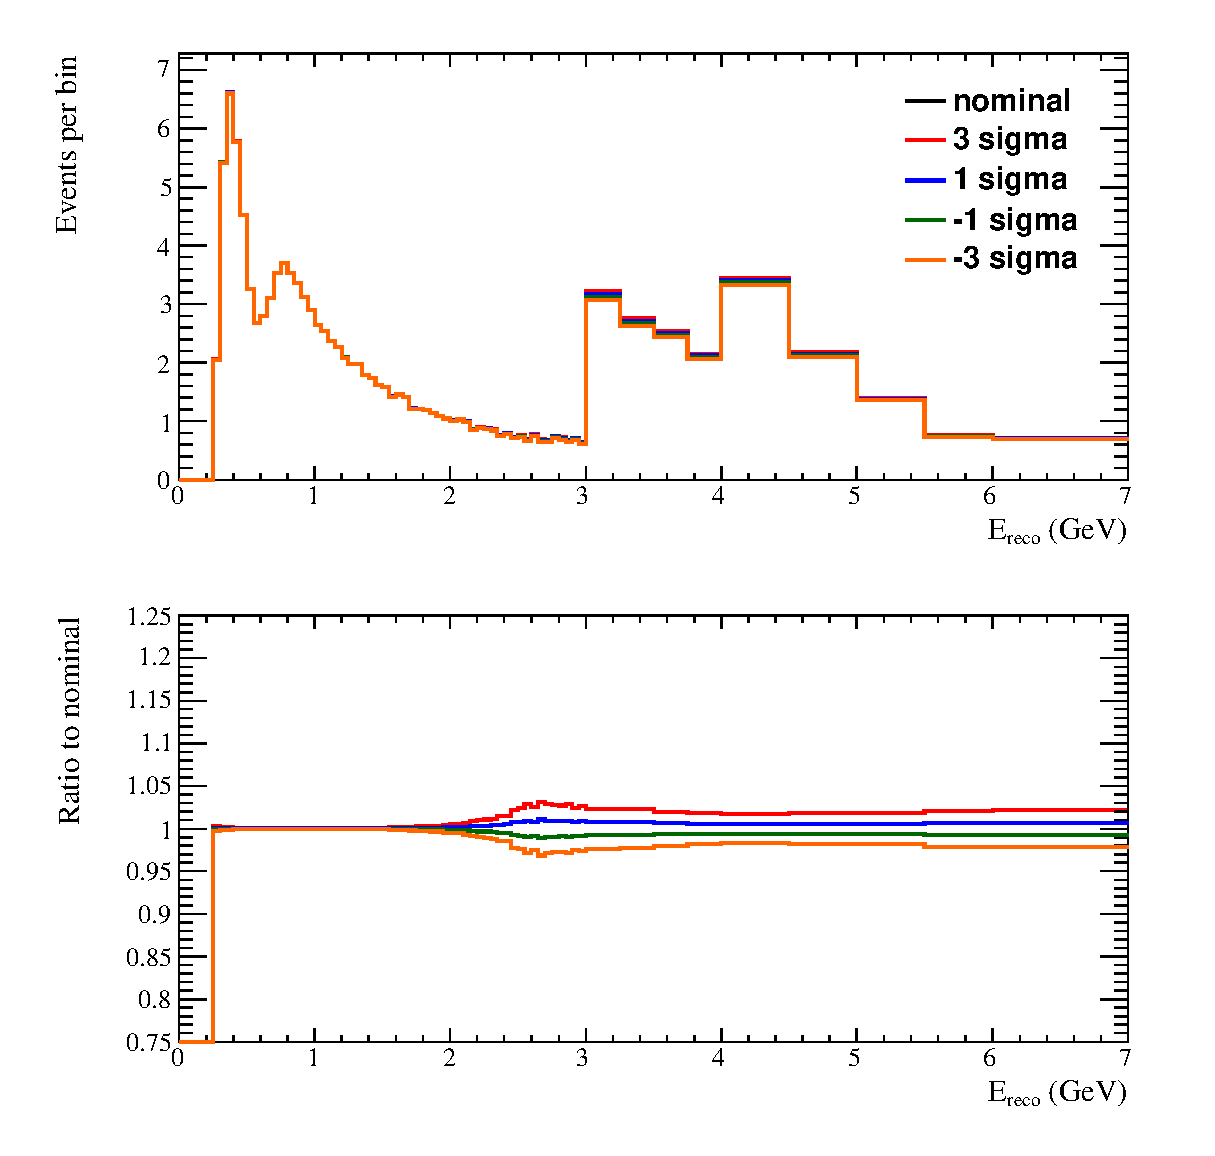
\includegraphics{../images/spectrum_tweaked/1sigma_oscillated/ereco_twk_f_banff15}}
\caption
{ Effect of $f_{15; t, r}^{banff}$ for 3 flavour oscillations, using oscillation parameters:  $\sin^2\theta_{12} = $0.306; $\sin^2\theta_{13} = $0.0251; $\sin^2\theta_{23} = $0.5; $\delta_{CP} = $        0; $\Delta m^2_{21} = $    7.5e-05 eV$^2$/c$^4$; $|\Delta m^2_{32}| = $    0.0024 eV$^2$/c$^4$. }
\label{fig:osc_ereco_twk_f_banff15}
\end{center}
\end{figure}
\clearpage

\begin{figure}
\begin{center}
\resizebox{14cm}{!}{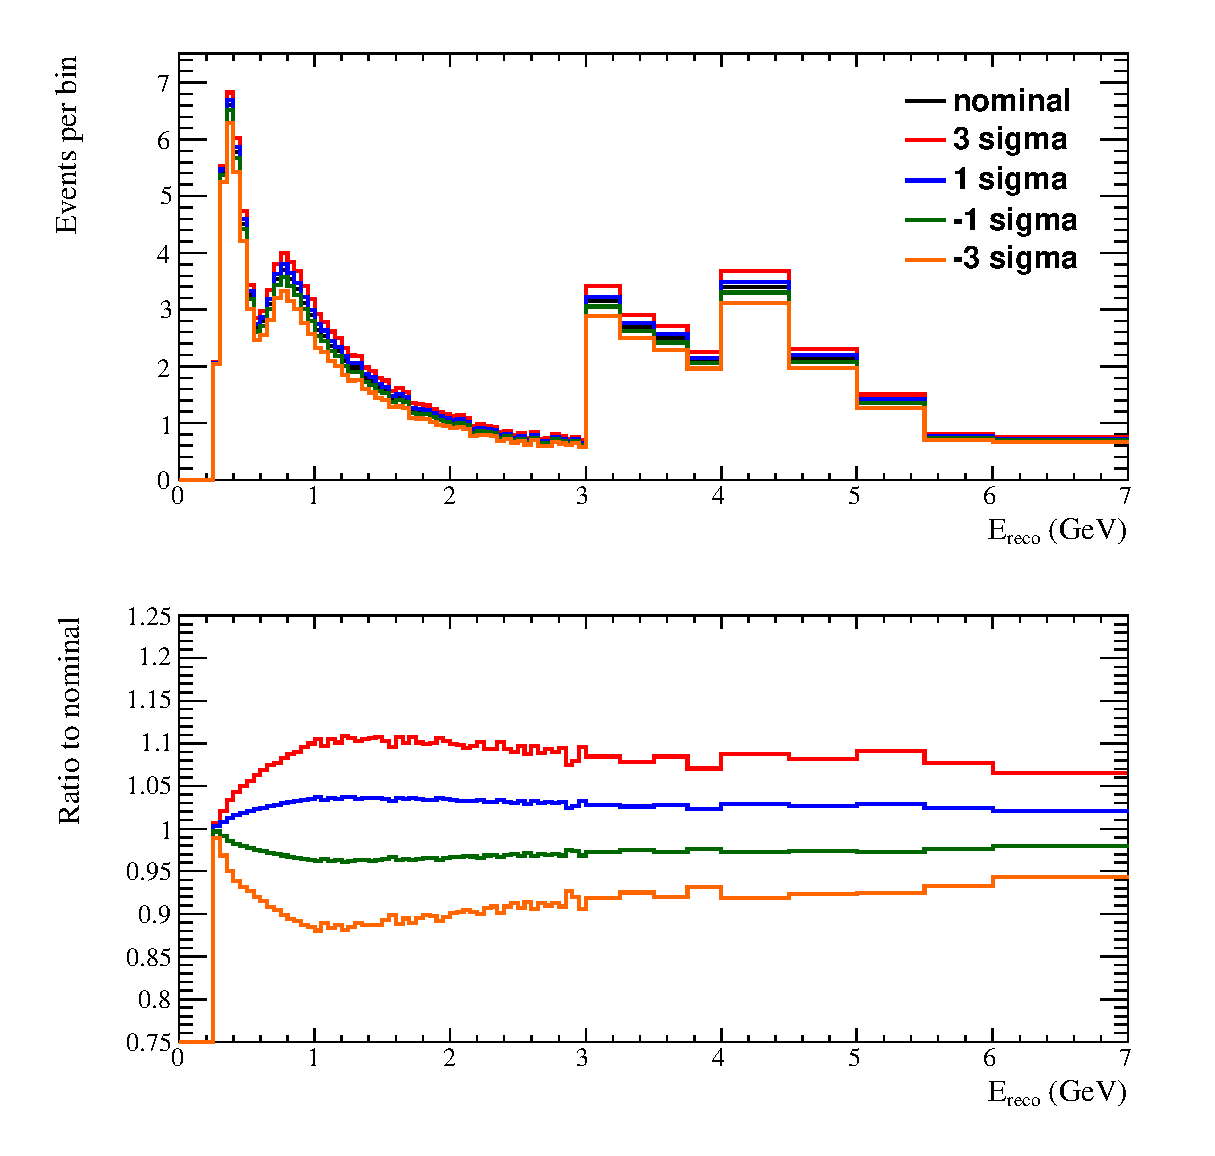
\includegraphics{../images/spectrum_tweaked/1sigma_oscillated/ereco_twk_f_banffmaqe}}
\caption
{ Effect of $f_{16; t, r}^{banff}$ for 3 flavour oscillations, using oscillation parameters:  $\sin^2\theta_{12} = $0.306; $\sin^2\theta_{13} = $0.0251; $\sin^2\theta_{23} = $0.5; $\delta_{CP} = $        0; $\Delta m^2_{21} = $    7.5e-05 eV$^2$/c$^4$; $|\Delta m^2_{32}| = $    0.0024 eV$^2$/c$^4$. }
\label{fig:osc_ereco_twk_f_banffmaqe}
\end{center}
\end{figure}
\clearpage

\begin{figure}
\begin{center}
\resizebox{14cm}{!}{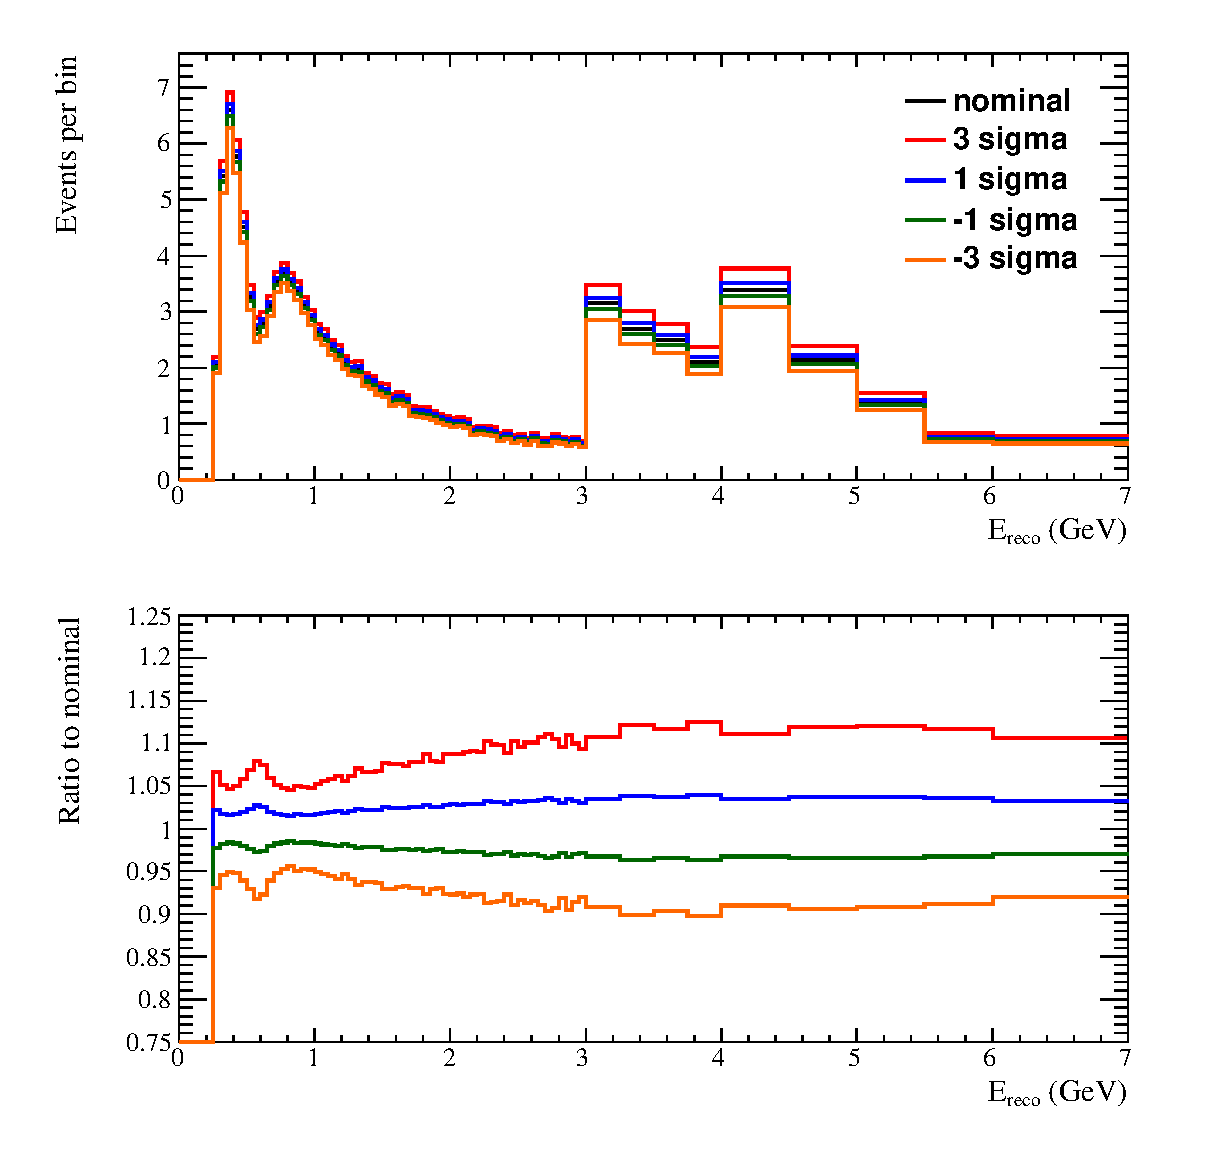
\includegraphics{../images/spectrum_tweaked/1sigma_oscillated/ereco_twk_f_banffmares}}
\caption
{ Effect of $f_{17; t, r}^{banff}$ for 3 flavour oscillations, using oscillation parameters:  $\sin^2\theta_{12} = $0.306; $\sin^2\theta_{13} = $0.0251; $\sin^2\theta_{23} = $0.5; $\delta_{CP} = $        0; $\Delta m^2_{21} = $    7.5e-05 eV$^2$/c$^4$; $|\Delta m^2_{32}| = $    0.0024 eV$^2$/c$^4$. }
\label{fig:osc_ereco_twk_f_banffmares}
\end{center}
\end{figure}
\clearpage

\begin{figure}
\begin{center}
\resizebox{14cm}{!}{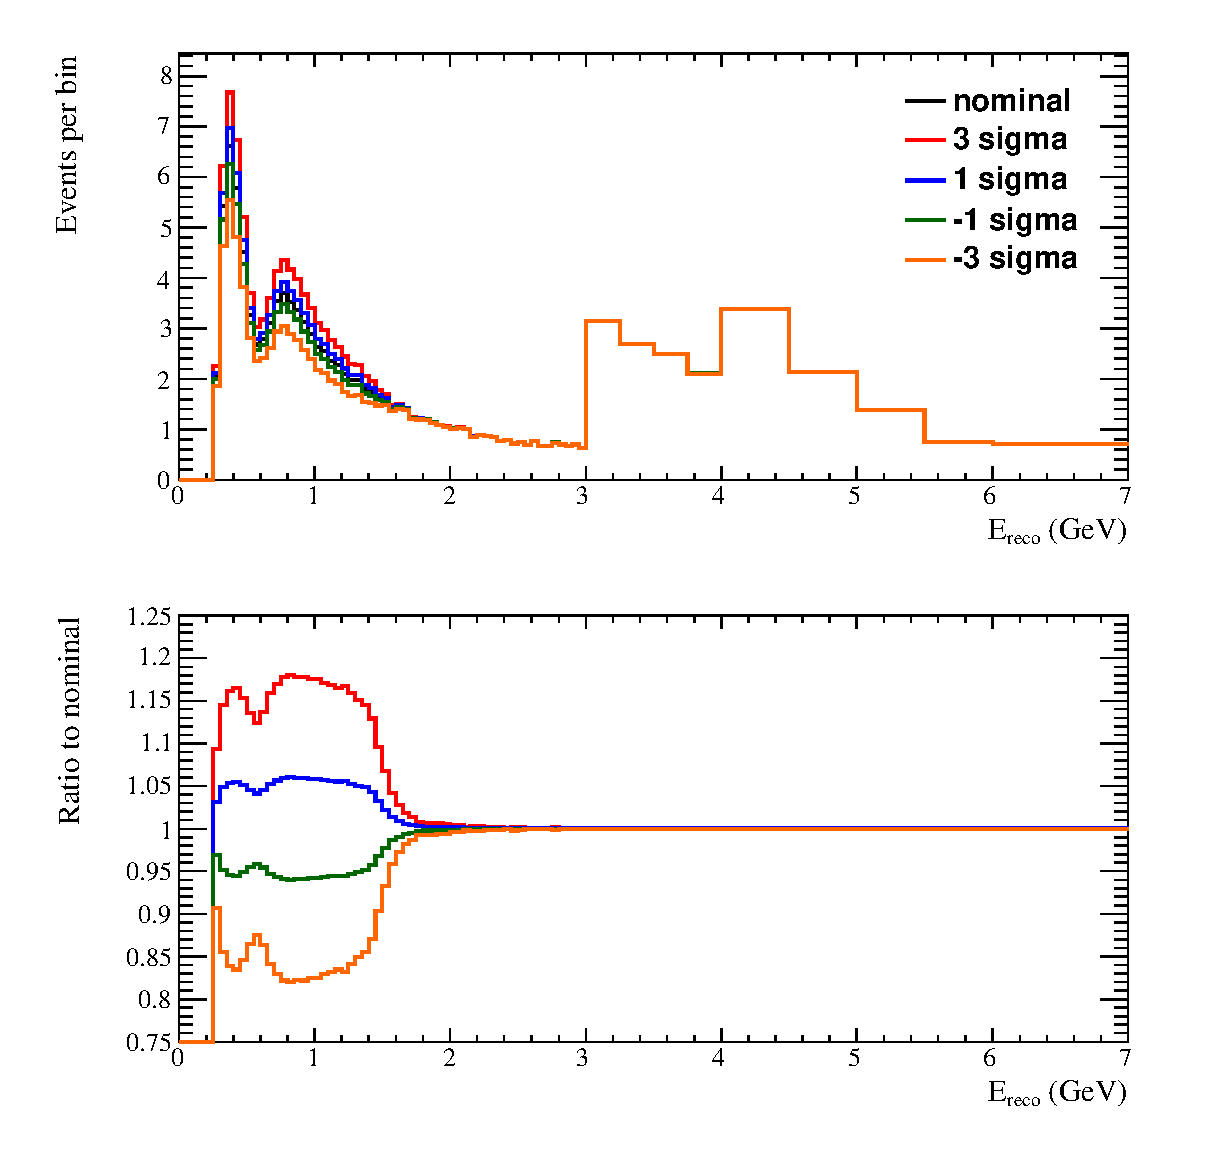
\includegraphics{../images/spectrum_tweaked/1sigma_oscillated/ereco_twk_f_banffccqee0}}
\caption
{ Effect of $f_{18; t, r}^{banff}$ for 3 flavour oscillations, using oscillation parameters:  $\sin^2\theta_{12} = $0.306; $\sin^2\theta_{13} = $0.0251; $\sin^2\theta_{23} = $0.5; $\delta_{CP} = $        0; $\Delta m^2_{21} = $    7.5e-05 eV$^2$/c$^4$; $|\Delta m^2_{32}| = $    0.0024 eV$^2$/c$^4$. }
\label{fig:osc_ereco_twk_f_banffccqee0}
\end{center}
\end{figure}
\clearpage

\begin{figure}
\begin{center}
\resizebox{14cm}{!}{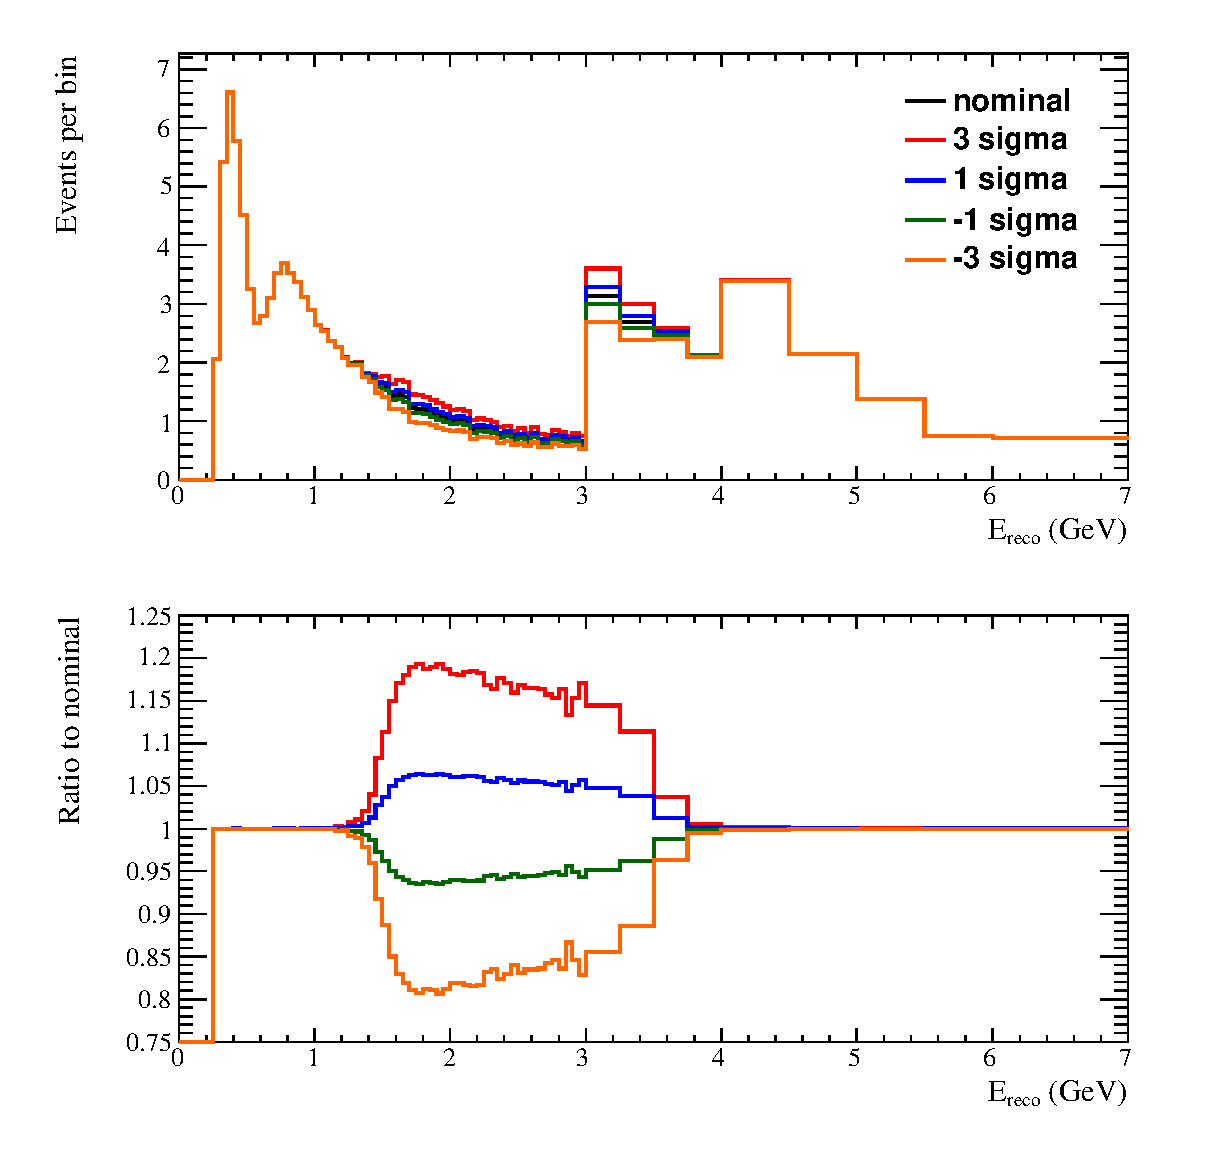
\includegraphics{../images/spectrum_tweaked/1sigma_oscillated/ereco_twk_f_banffccqee1}}
\caption
{ Effect of $f_{19; t, r}^{banff}$ for 3 flavour oscillations, using oscillation parameters:  $\sin^2\theta_{12} = $0.306; $\sin^2\theta_{13} = $0.0251; $\sin^2\theta_{23} = $0.5; $\delta_{CP} = $        0; $\Delta m^2_{21} = $    7.5e-05 eV$^2$/c$^4$; $|\Delta m^2_{32}| = $    0.0024 eV$^2$/c$^4$. }
\label{fig:osc_ereco_twk_f_banffccqee1}
\end{center}
\end{figure}
\clearpage

\begin{figure}
\begin{center}
\resizebox{14cm}{!}{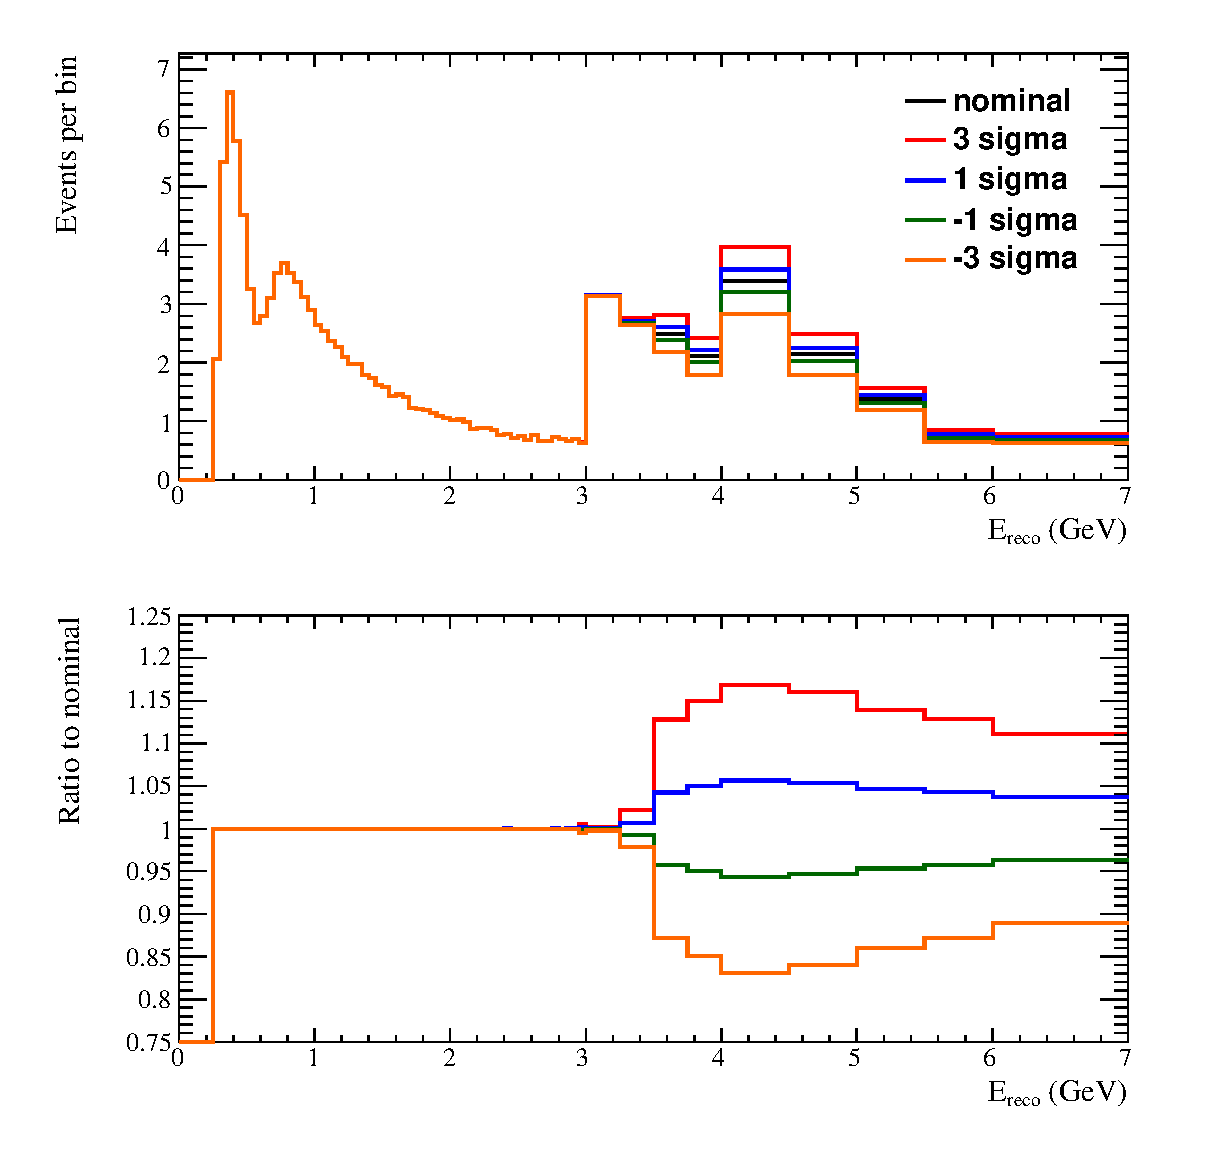
\includegraphics{../images/spectrum_tweaked/1sigma_oscillated/ereco_twk_f_banffccqee2}}
\caption
{ Effect of $f_{20; t, r}^{banff}$ for 3 flavour oscillations, using oscillation parameters:  $\sin^2\theta_{12} = $0.306; $\sin^2\theta_{13} = $0.0251; $\sin^2\theta_{23} = $0.5; $\delta_{CP} = $        0; $\Delta m^2_{21} = $    7.5e-05 eV$^2$/c$^4$; $|\Delta m^2_{32}| = $    0.0024 eV$^2$/c$^4$. }
\label{fig:osc_ereco_twk_f_banffccqee2}
\end{center}
\end{figure}
\clearpage

\begin{figure}
\begin{center}
\resizebox{14cm}{!}{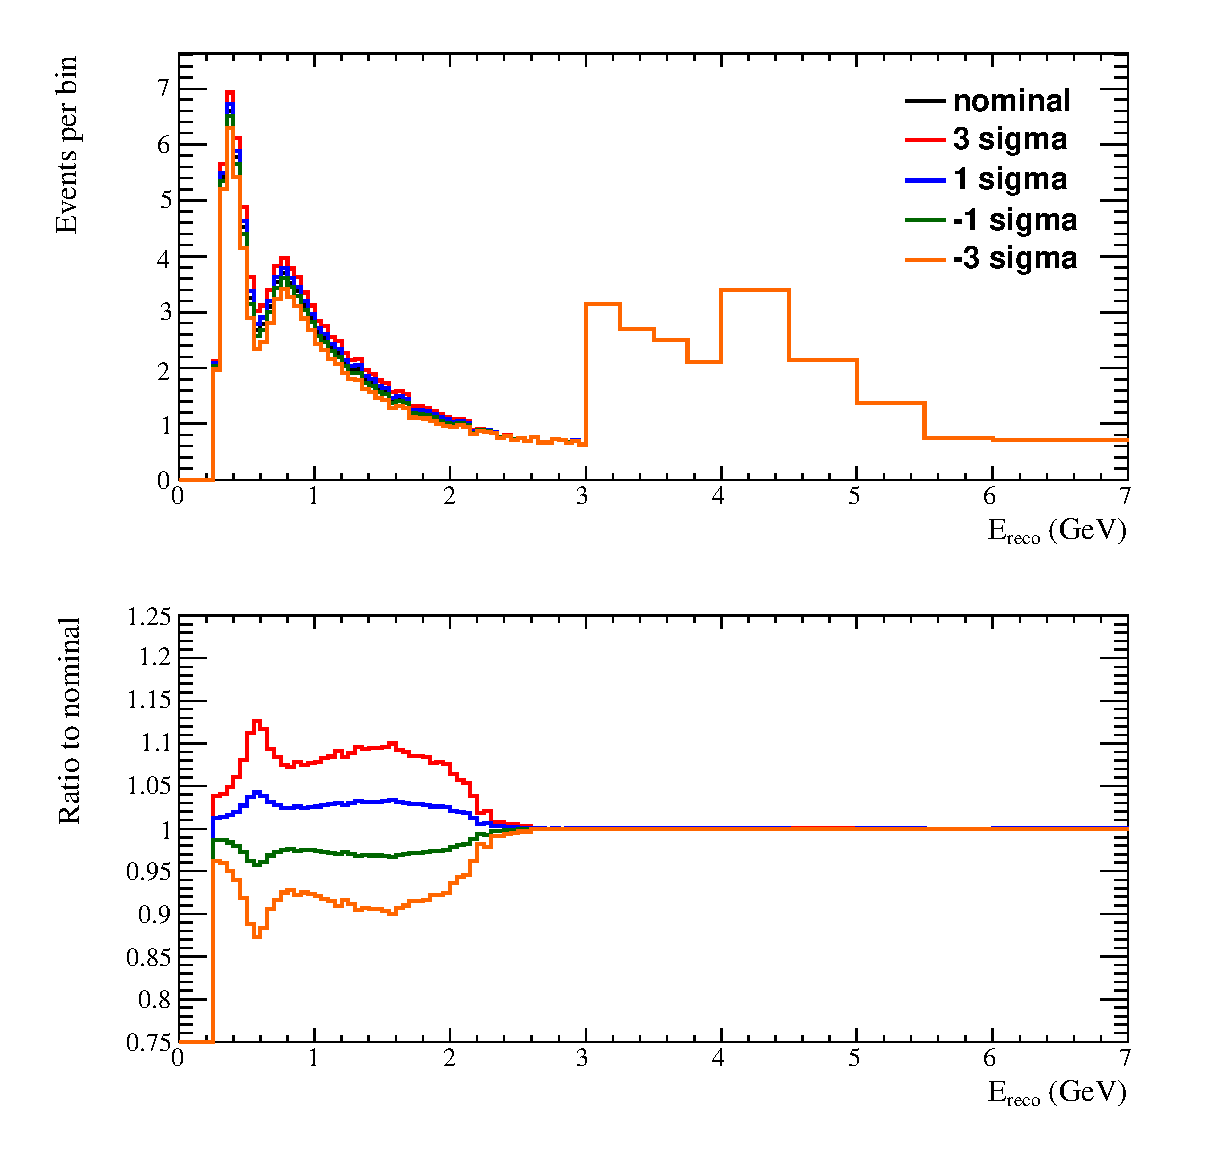
\includegraphics{../images/spectrum_tweaked/1sigma_oscillated/ereco_twk_f_banffcc1pie0}}
\caption
{ Effect of $f_{21; t, r}^{banff}$ for 3 flavour oscillations, using oscillation parameters:  $\sin^2\theta_{12} = $0.306; $\sin^2\theta_{13} = $0.0251; $\sin^2\theta_{23} = $0.5; $\delta_{CP} = $        0; $\Delta m^2_{21} = $    7.5e-05 eV$^2$/c$^4$; $|\Delta m^2_{32}| = $    0.0024 eV$^2$/c$^4$. }
\label{fig:osc_ereco_twk_f_banffcc1pie0}
\end{center}
\end{figure}
\clearpage

\begin{figure}
\begin{center}
\resizebox{14cm}{!}{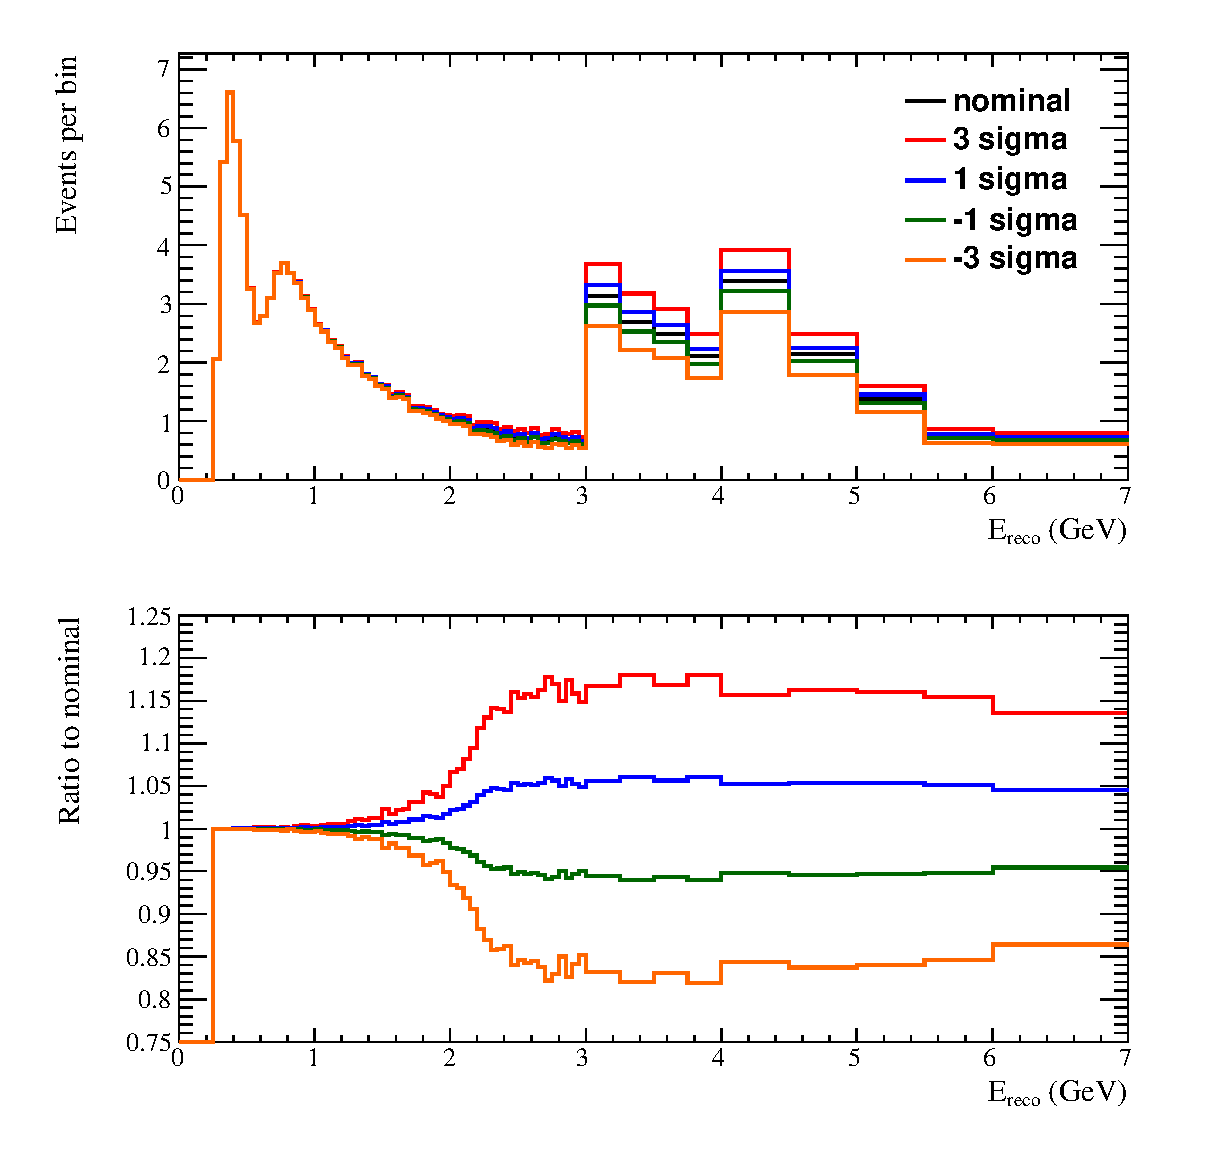
\includegraphics{../images/spectrum_tweaked/1sigma_oscillated/ereco_twk_f_banffcc1pie1}}
\caption
{ Effect of $f_{22; t, r}^{banff}$ for 3 flavour oscillations, using oscillation parameters:  $\sin^2\theta_{12} = $0.306; $\sin^2\theta_{13} = $0.0251; $\sin^2\theta_{23} = $0.5; $\delta_{CP} = $        0; $\Delta m^2_{21} = $    7.5e-05 eV$^2$/c$^4$; $|\Delta m^2_{32}| = $    0.0024 eV$^2$/c$^4$. }
\label{fig:osc_ereco_twk_f_banffcc1pie1}
\end{center}
\end{figure}
\clearpage

\begin{figure}
\begin{center}
\resizebox{14cm}{!}{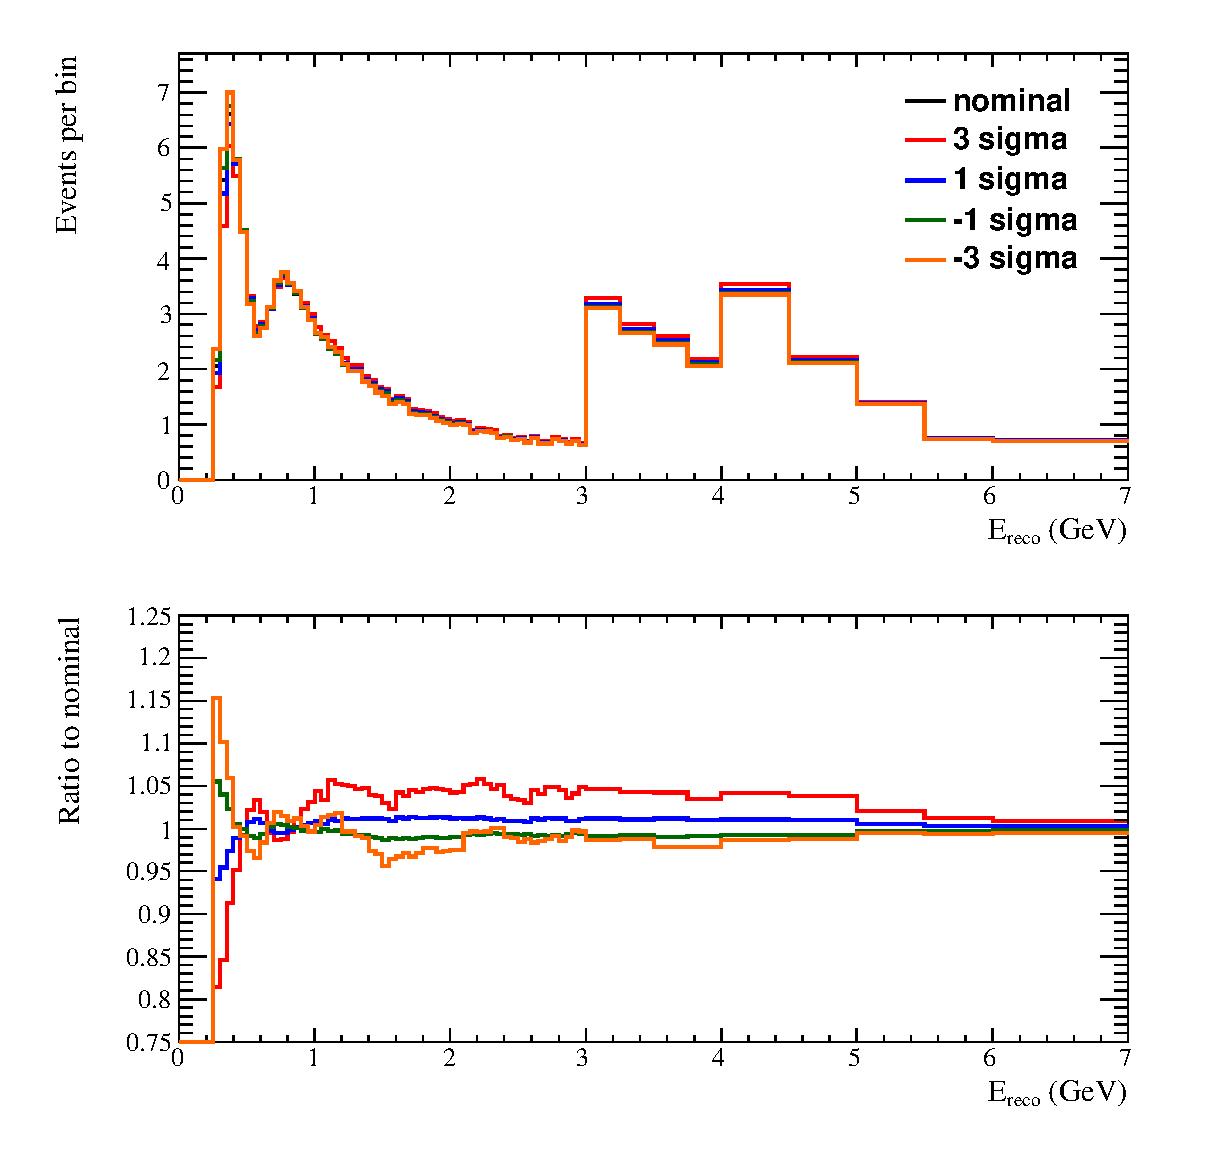
\includegraphics{../images/spectrum_tweaked/1sigma_oscillated/ereco_twk_f_pfermi}}
\caption
{ Effect of $f_{pF; t, r}$ for 3 flavour oscillations, using oscillation parameters:  $\sin^2\theta_{12} = $0.306; $\sin^2\theta_{13} = $0.0251; $\sin^2\theta_{23} = $0.5; $\delta_{CP} = $        0; $\Delta m^2_{21} = $    7.5e-05 eV$^2$/c$^4$; $|\Delta m^2_{32}| = $    0.0024 eV$^2$/c$^4$. }
\label{fig:osc_ereco_twk_f_pfermi}
\end{center}
\end{figure}
\clearpage

\begin{figure}
\begin{center}
\resizebox{14cm}{!}{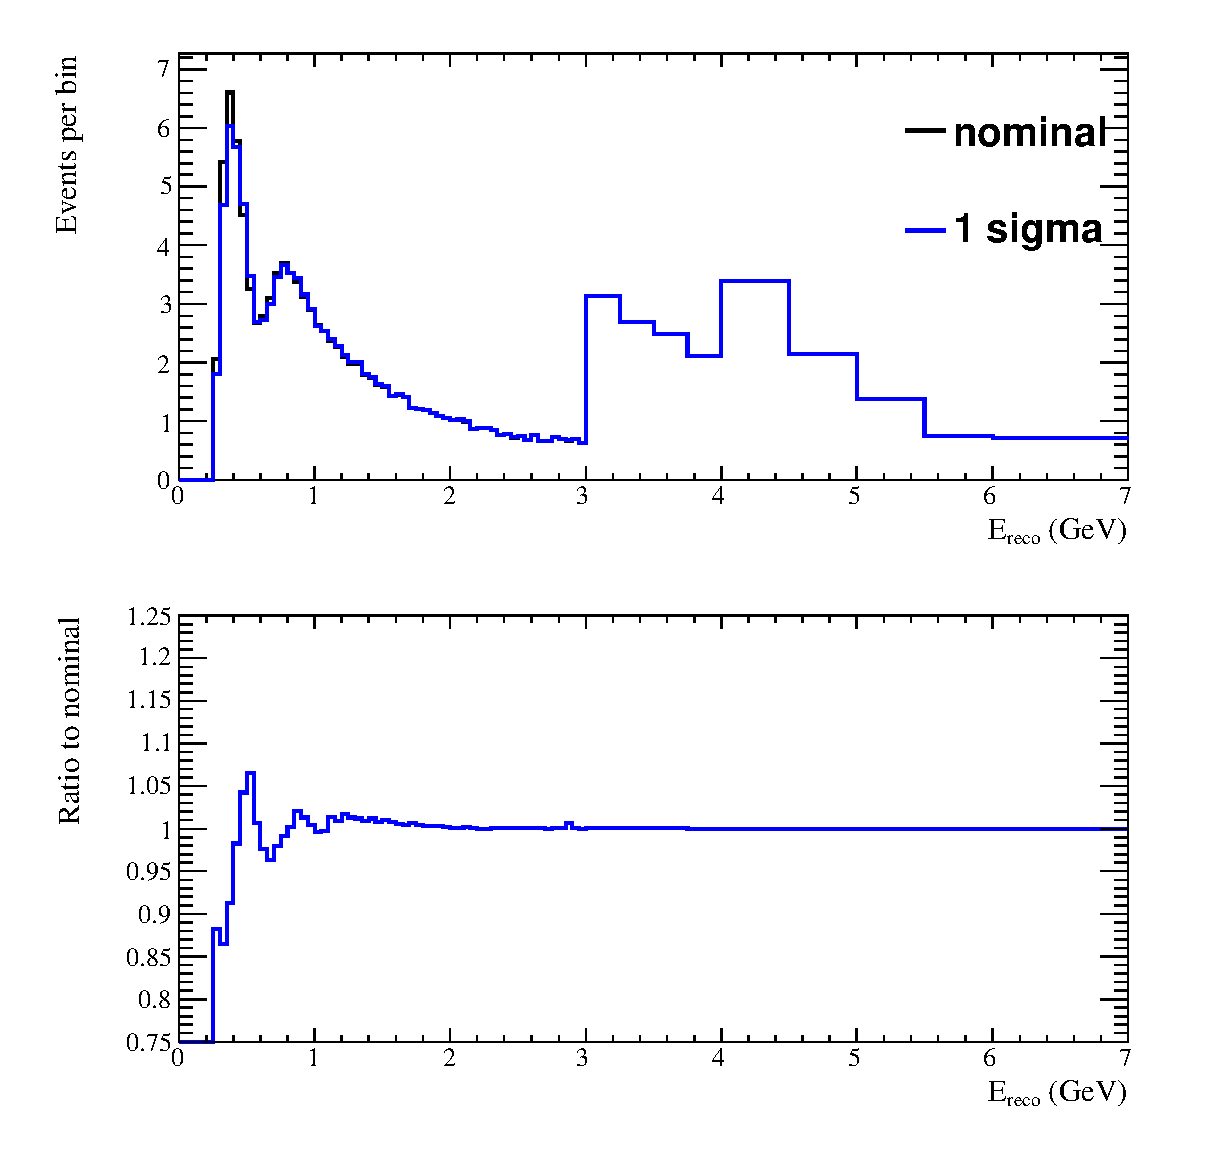
\includegraphics{../images/spectrum_tweaked/1sigma_oscillated/ereco_twk_f_specfunc}}
\caption
{ Effect of $f_{SF; t, r}$ for 3 flavour oscillations, using oscillation parameters:  $\sin^2\theta_{12} = $0.306; $\sin^2\theta_{13} = $0.0251; $\sin^2\theta_{23} = $0.5; $\delta_{CP} = $        0; $\Delta m^2_{21} = $    7.5e-05 eV$^2$/c$^4$; $|\Delta m^2_{32}| = $    0.0024 eV$^2$/c$^4$. }
\label{fig:osc_ereco_twk_f_specfunc}
\end{center}
\end{figure}
\clearpage

\begin{figure}
\begin{center}
\resizebox{14cm}{!}{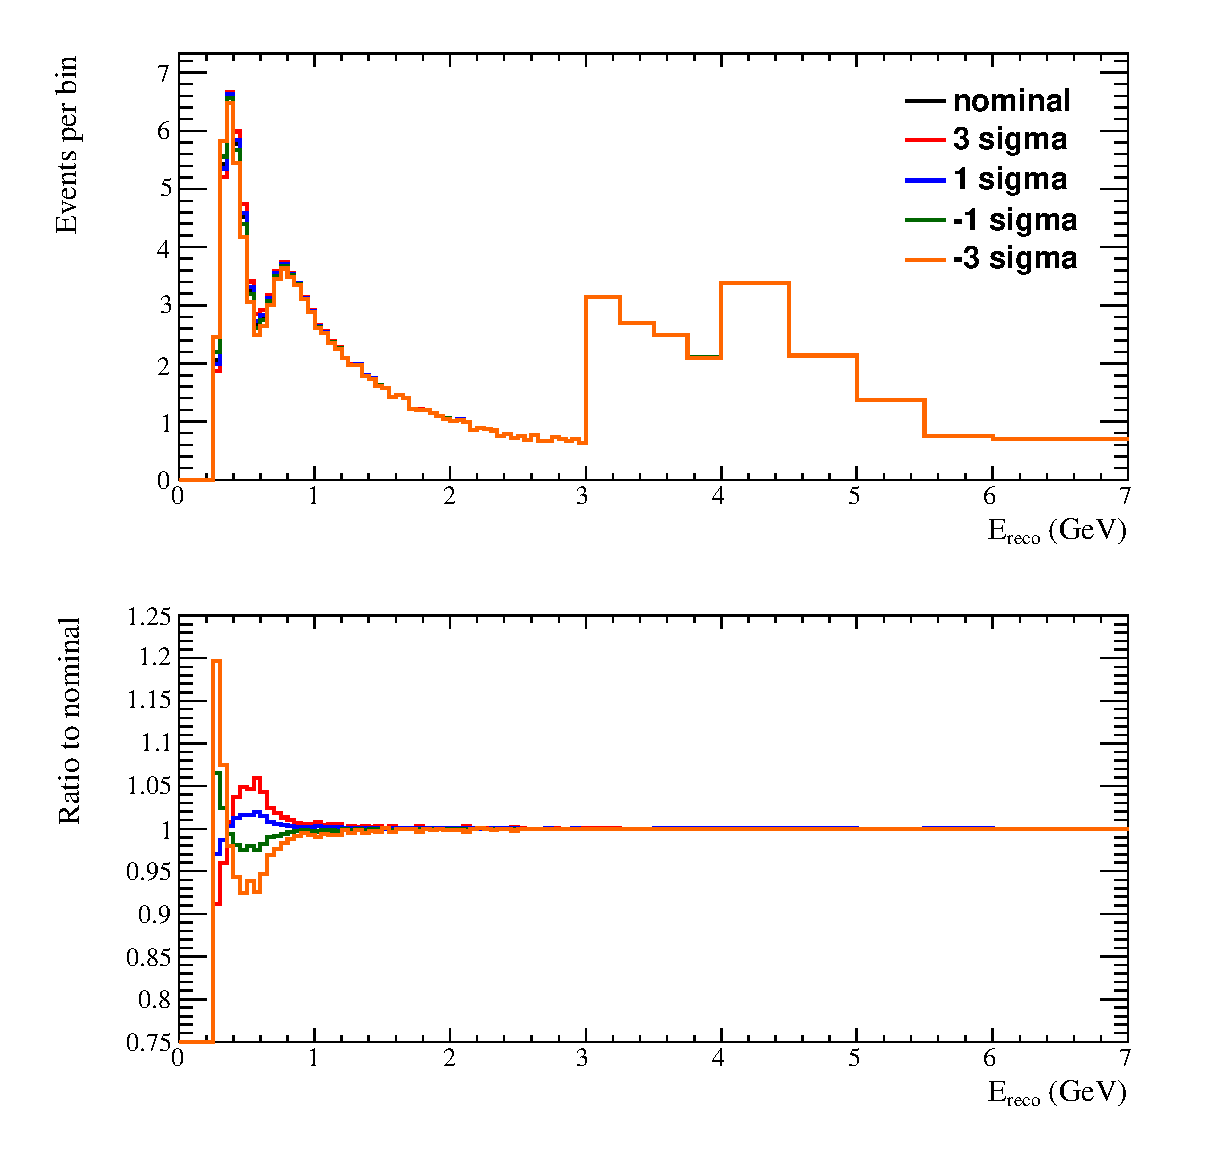
\includegraphics{../images/spectrum_tweaked/1sigma_oscillated/ereco_twk_f_wshape}}
\caption
{ Effect of $f_{Wshape; t, r}$ for 3 flavour oscillations, using oscillation parameters:  $\sin^2\theta_{12} = $0.306; $\sin^2\theta_{13} = $0.0251; $\sin^2\theta_{23} = $0.5; $\delta_{CP} = $        0; $\Delta m^2_{21} = $    7.5e-05 eV$^2$/c$^4$; $|\Delta m^2_{32}| = $    0.0024 eV$^2$/c$^4$. }
\label{fig:osc_ereco_twk_f_wshape}
\end{center}
\end{figure}
\clearpage

\begin{figure}
\begin{center}
\resizebox{14cm}{!}{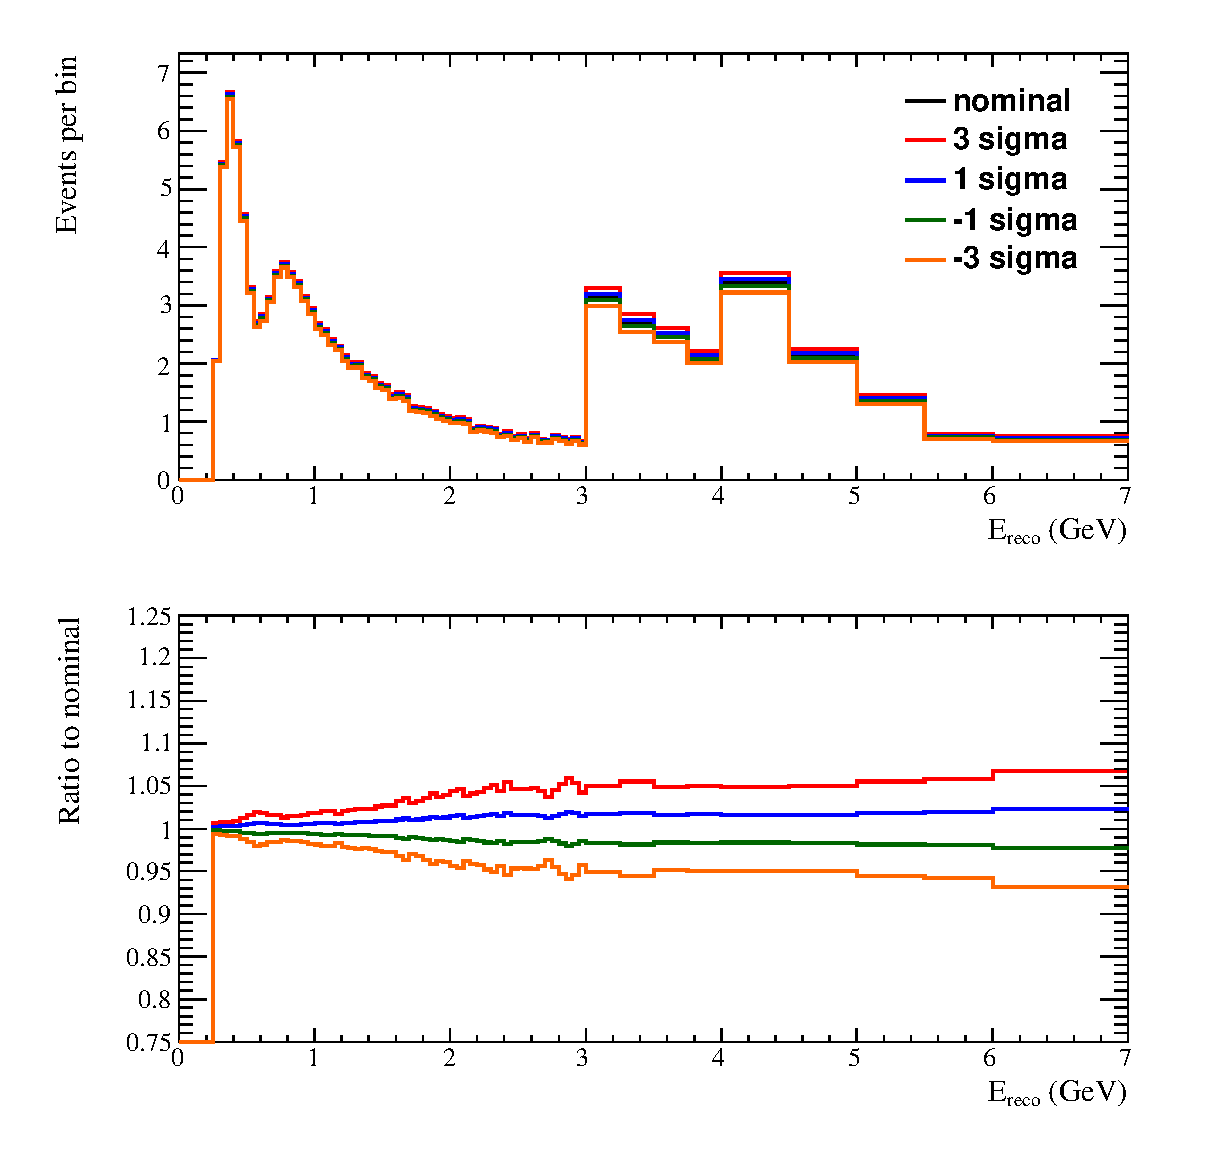
\includegraphics{../images/spectrum_tweaked/1sigma_oscillated/ereco_twk_f_shapeCCoth}}
\caption
{ Effect of $f_{CCothShape; t, r}$ for 3 flavour oscillations, using oscillation parameters:  $\sin^2\theta_{12} = $0.306; $\sin^2\theta_{13} = $0.0251; $\sin^2\theta_{23} = $0.5; $\delta_{CP} = $        0; $\Delta m^2_{21} = $    7.5e-05 eV$^2$/c$^4$; $|\Delta m^2_{32}| = $    0.0024 eV$^2$/c$^4$. }
\label{fig:osc_ereco_twk_f_shapeCCoth}
\end{center}
\end{figure}
\clearpage

\begin{figure}
\begin{center}
\resizebox{14cm}{!}{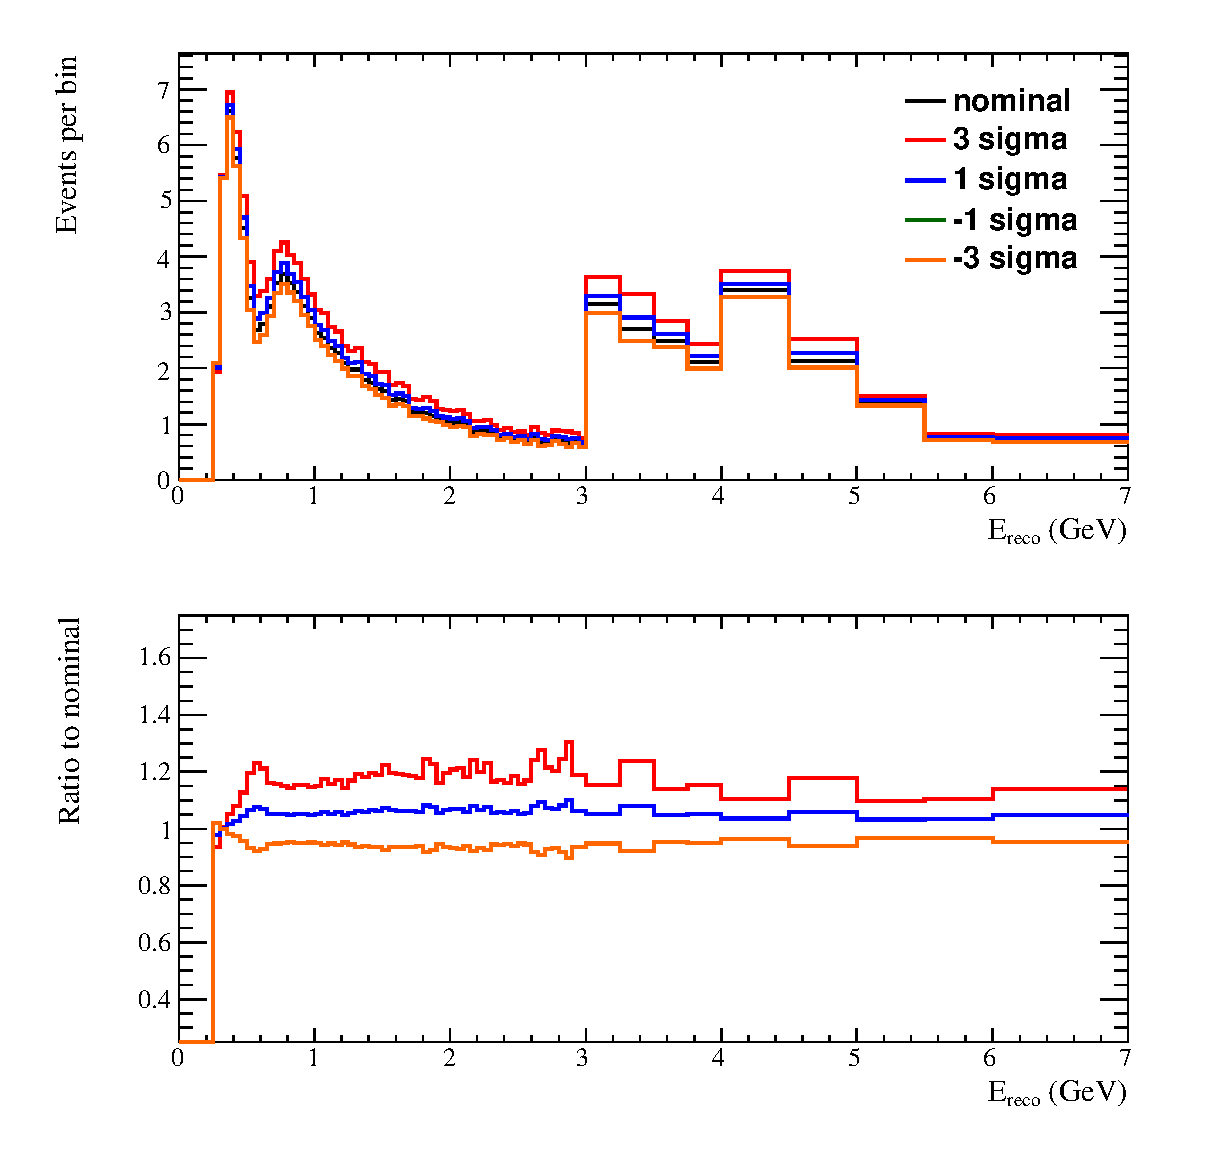
\includegraphics{../images/spectrum_tweaked/1sigma_oscillated/ereco_twk_f_pilessdelta}}
\caption
{ Effect of $f_{\pi-less\Delta; t, r}$ for 3 flavour oscillations, using oscillation parameters:  $\sin^2\theta_{12} = $0.306; $\sin^2\theta_{13} = $0.0251; $\sin^2\theta_{23} = $0.5; $\delta_{CP} = $        0; $\Delta m^2_{21} = $    7.5e-05 eV$^2$/c$^4$; $|\Delta m^2_{32}| = $    0.0024 eV$^2$/c$^4$. }
\label{fig:osc_ereco_twk_f_pilessdelta}
\end{center}
\end{figure}
\clearpage

\begin{figure}
\begin{center}
\resizebox{14cm}{!}{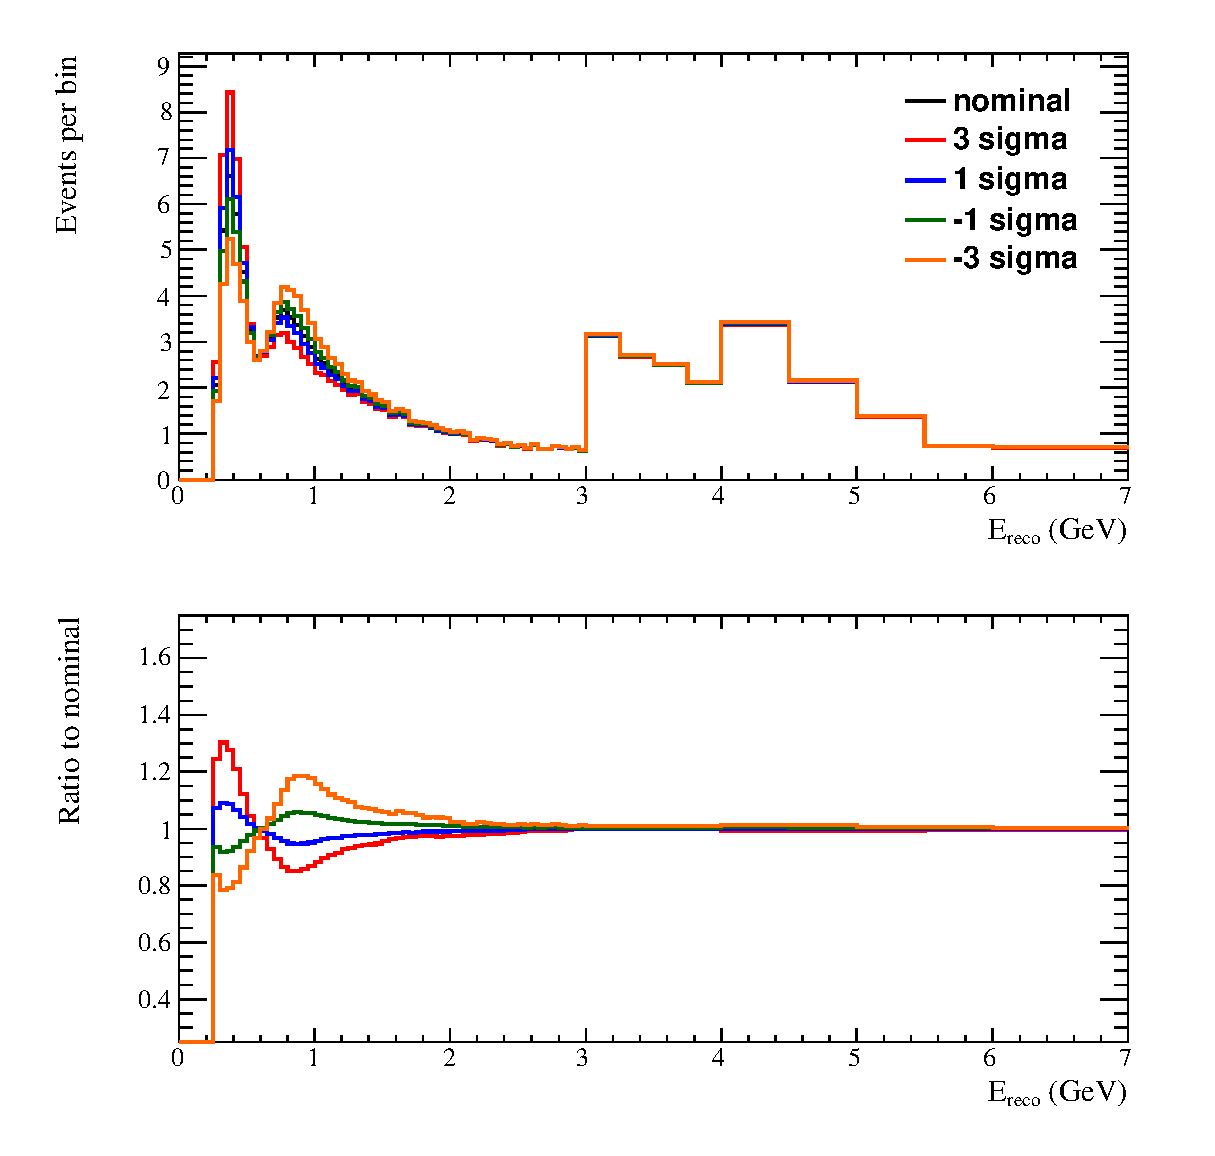
\includegraphics{../images/spectrum_tweaked/1sigma_oscillated/ereco_twk_f_bindE}}
\caption
{ Effect of $f_{bindE; t, r}$ for 3 flavour oscillations, using oscillation parameters:  $\sin^2\theta_{12} = $0.306; $\sin^2\theta_{13} = $0.0251; $\sin^2\theta_{23} = $0.5; $\delta_{CP} = $        0; $\Delta m^2_{21} = $    7.5e-05 eV$^2$/c$^4$; $|\Delta m^2_{32}| = $    0.0024 eV$^2$/c$^4$. }
\label{fig:osc_ereco_twk_f_bindE}
\end{center}
\end{figure}
\clearpage

\begin{figure}
\begin{center}
\resizebox{14cm}{!}{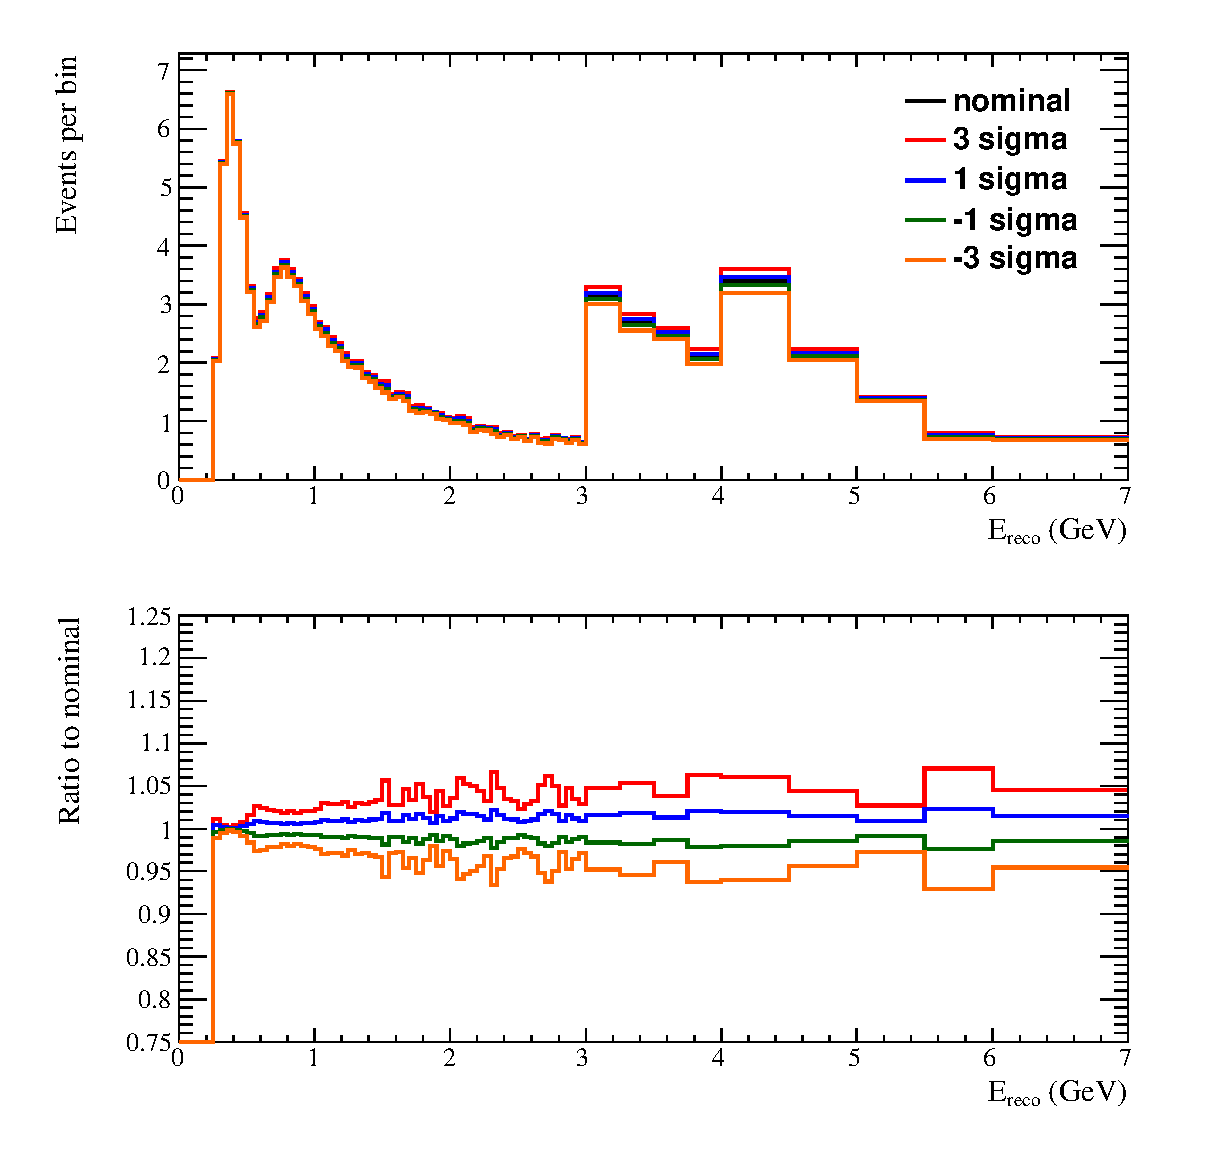
\includegraphics{../images/spectrum_tweaked/1sigma_oscillated/ereco_twk_f_norm_cccoh}}
\caption
{ Effect of $f_{CCcoh; t}$ for 3 flavour oscillations, using oscillation parameters:  $\sin^2\theta_{12} = $0.306; $\sin^2\theta_{13} = $0.0251; $\sin^2\theta_{23} = $0.5; $\delta_{CP} = $        0; $\Delta m^2_{21} = $    7.5e-05 eV$^2$/c$^4$; $|\Delta m^2_{32}| = $    0.0024 eV$^2$/c$^4$. }
\label{fig:osc_ereco_twk_f_norm_cccoh}
\end{center}
\end{figure}
\clearpage

\begin{figure}
\begin{center}
\resizebox{14cm}{!}{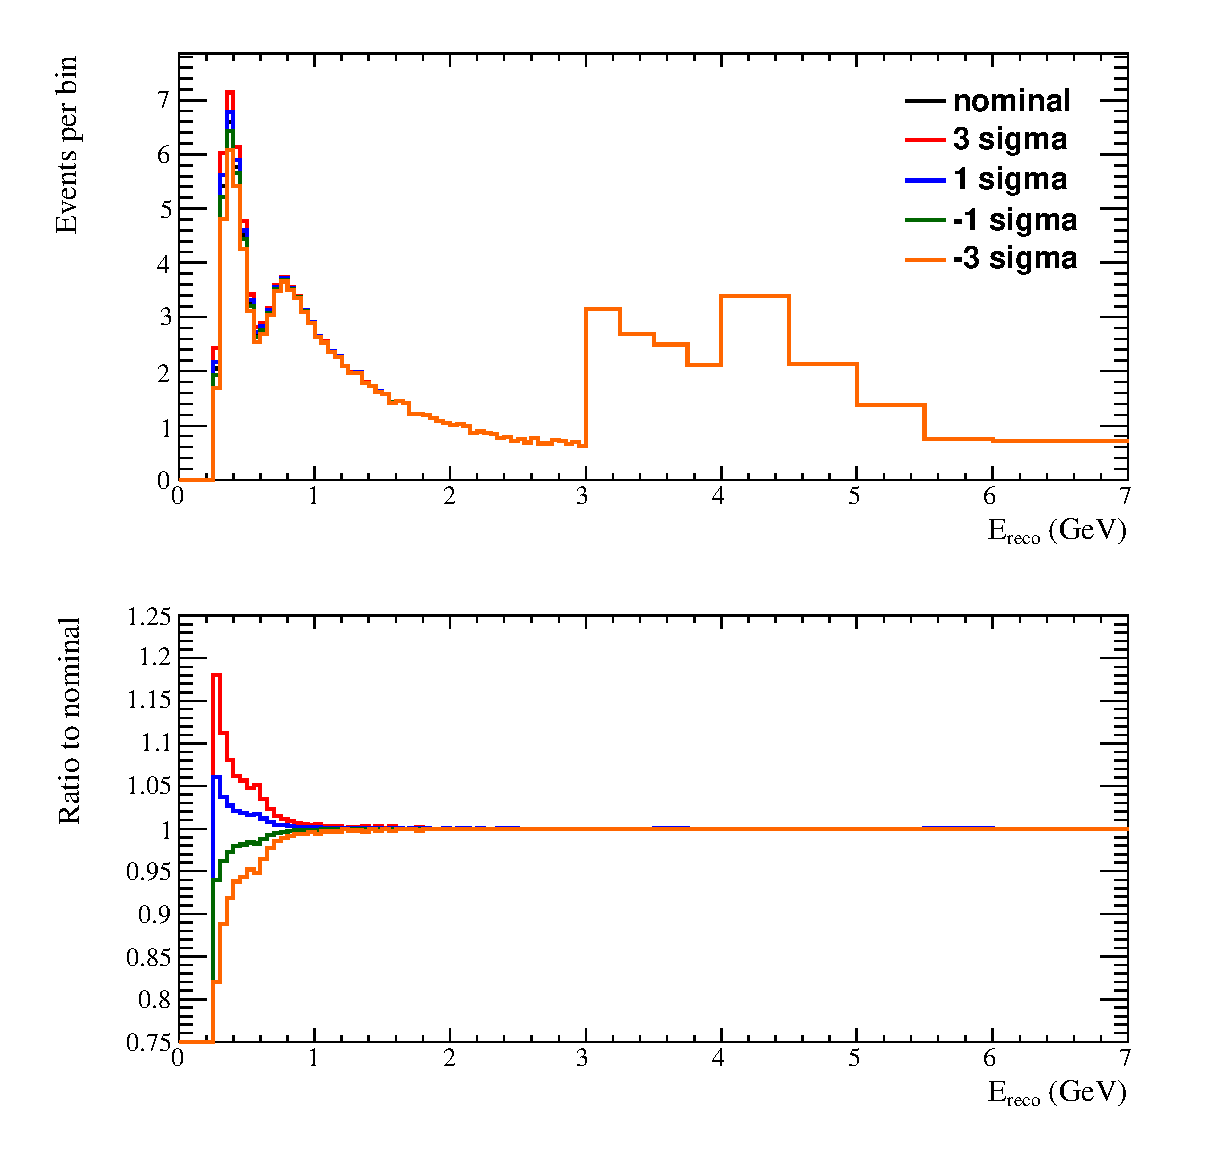
\includegraphics{../images/spectrum_tweaked/1sigma_oscillated/ereco_twk_f_norm_nc1piC}}
\caption
{ Effect of $f_{NC1\pi^\pm; t}$ for 3 flavour oscillations, using oscillation parameters:  $\sin^2\theta_{12} = $0.306; $\sin^2\theta_{13} = $0.0251; $\sin^2\theta_{23} = $0.5; $\delta_{CP} = $        0; $\Delta m^2_{21} = $    7.5e-05 eV$^2$/c$^4$; $|\Delta m^2_{32}| = $    0.0024 eV$^2$/c$^4$. }
\label{fig:osc_ereco_twk_f_norm_nc1piC}
\end{center}
\end{figure}
\clearpage

\begin{figure}
\begin{center}
\resizebox{14cm}{!}{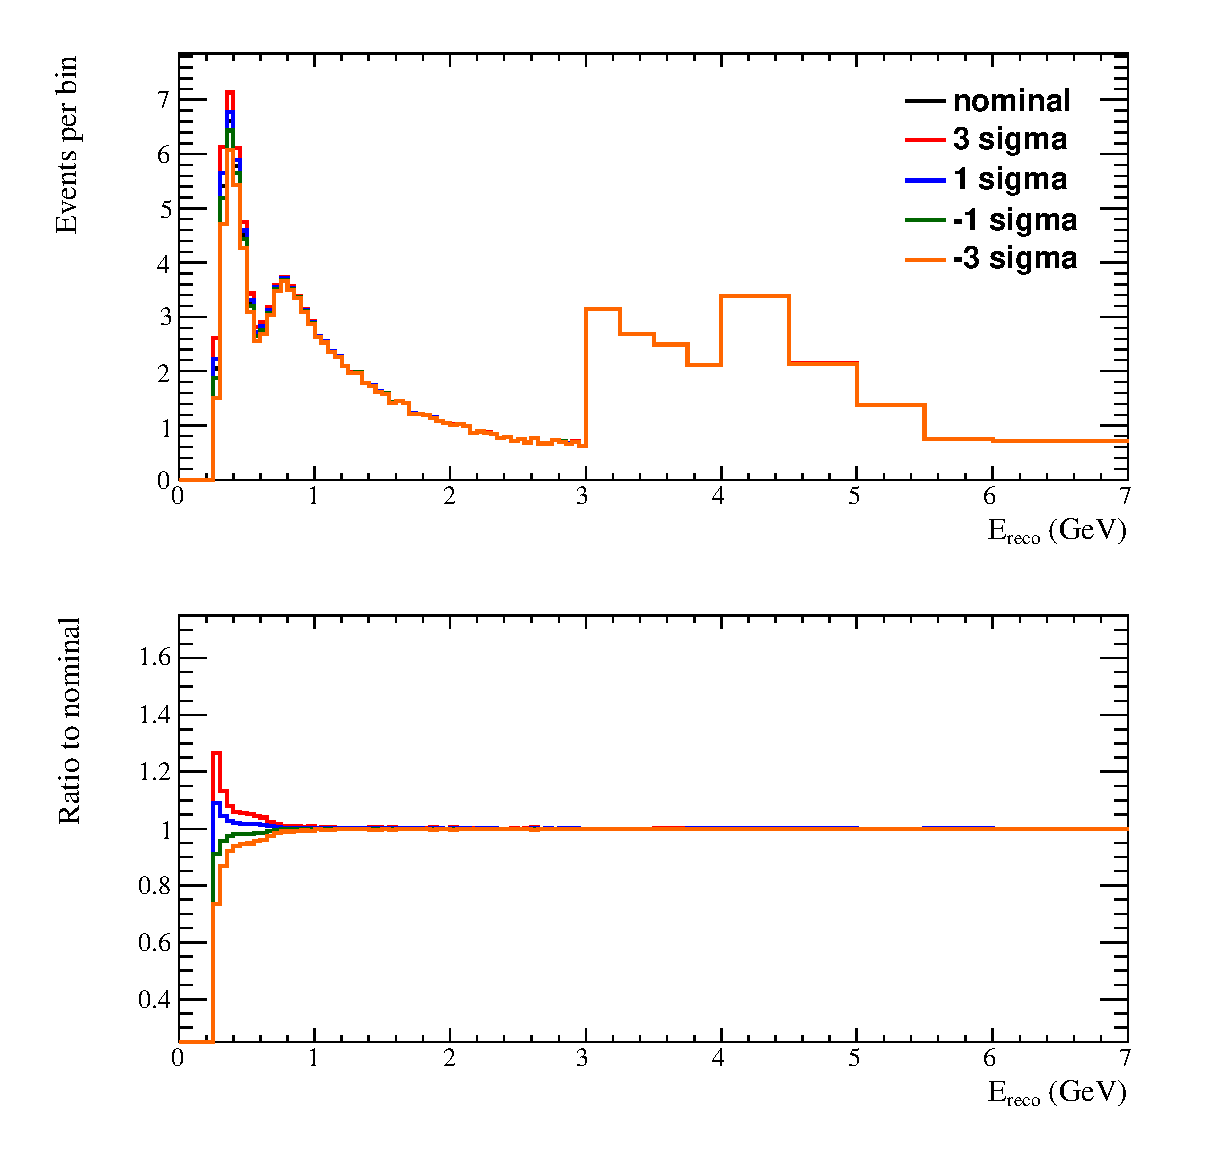
\includegraphics{../images/spectrum_tweaked/1sigma_oscillated/ereco_twk_f_norm_ncoth}}
\caption
{ Effect of $f_{NCoth; t}$ for 3 flavour oscillations, using oscillation parameters:  $\sin^2\theta_{12} = $0.306; $\sin^2\theta_{13} = $0.0251; $\sin^2\theta_{23} = $0.5; $\delta_{CP} = $        0; $\Delta m^2_{21} = $    7.5e-05 eV$^2$/c$^4$; $|\Delta m^2_{32}| = $    0.0024 eV$^2$/c$^4$. }
\label{fig:osc_ereco_twk_f_norm_ncoth}
\end{center}
\end{figure}
\clearpage

\begin{figure}
\begin{center}
\resizebox{14cm}{!}{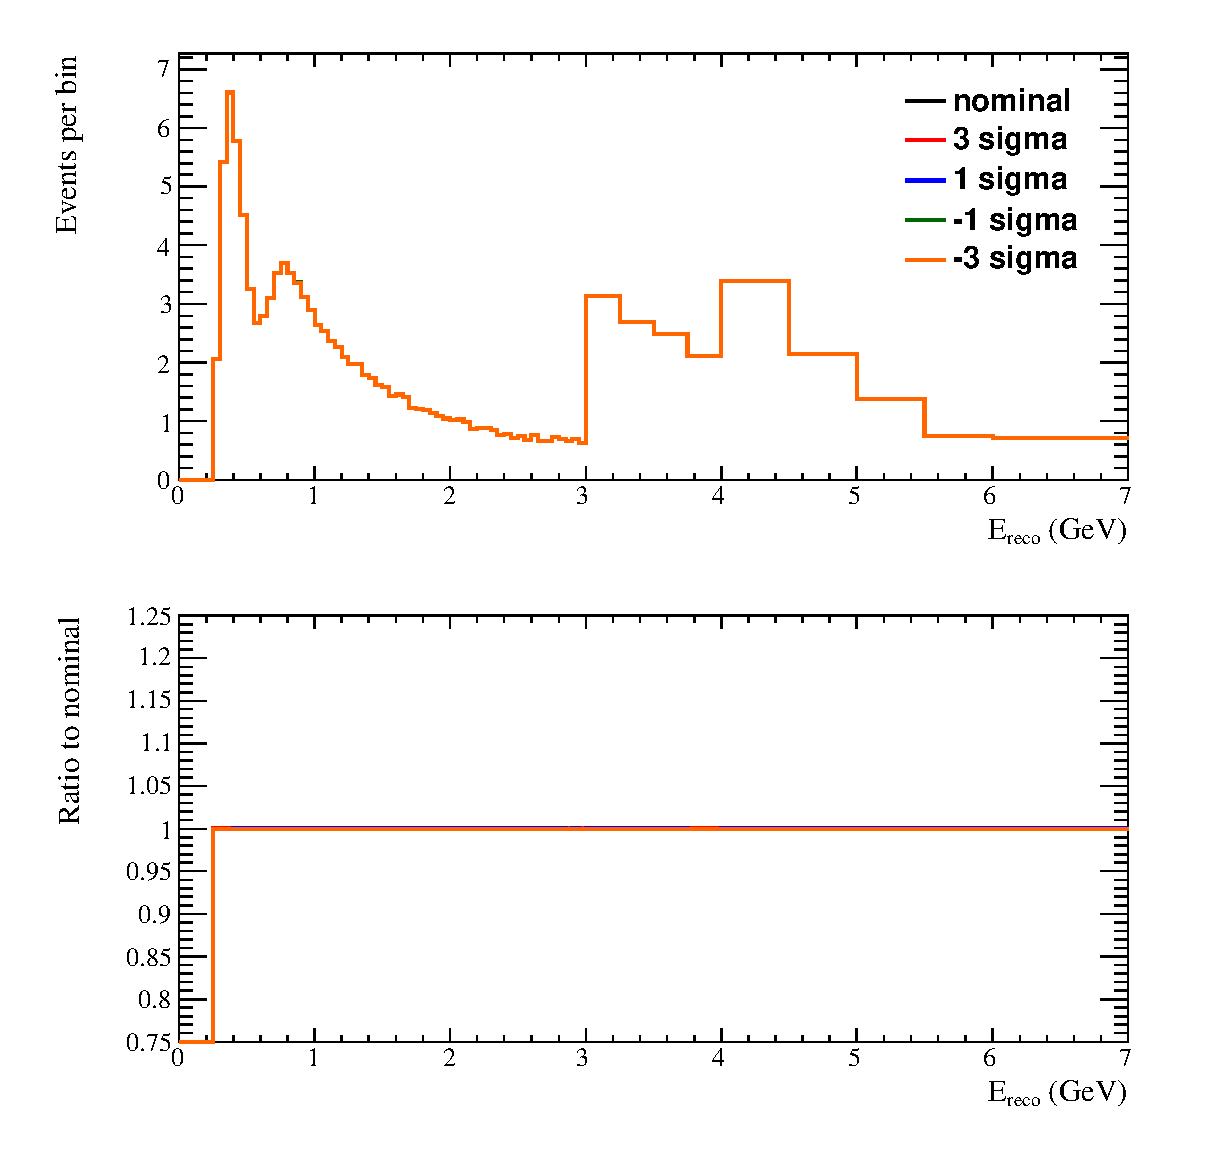
\includegraphics{../images/spectrum_tweaked/1sigma_oscillated/ereco_twk_f_norm_nuetonumu}}
\caption
{ Effect of $f_{CC\nu_e; t}$ for 3 flavour oscillations, using oscillation parameters:  $\sin^2\theta_{12} = $0.306; $\sin^2\theta_{13} = $0.0251; $\sin^2\theta_{23} = $0.5; $\delta_{CP} = $        0; $\Delta m^2_{21} = $    7.5e-05 eV$^2$/c$^4$; $|\Delta m^2_{32}| = $    0.0024 eV$^2$/c$^4$. }
\label{fig:osc_ereco_twk_f_norm_nuetonumu}
\end{center}
\end{figure}
\clearpage

\begin{figure}
\begin{center}
\resizebox{14cm}{!}{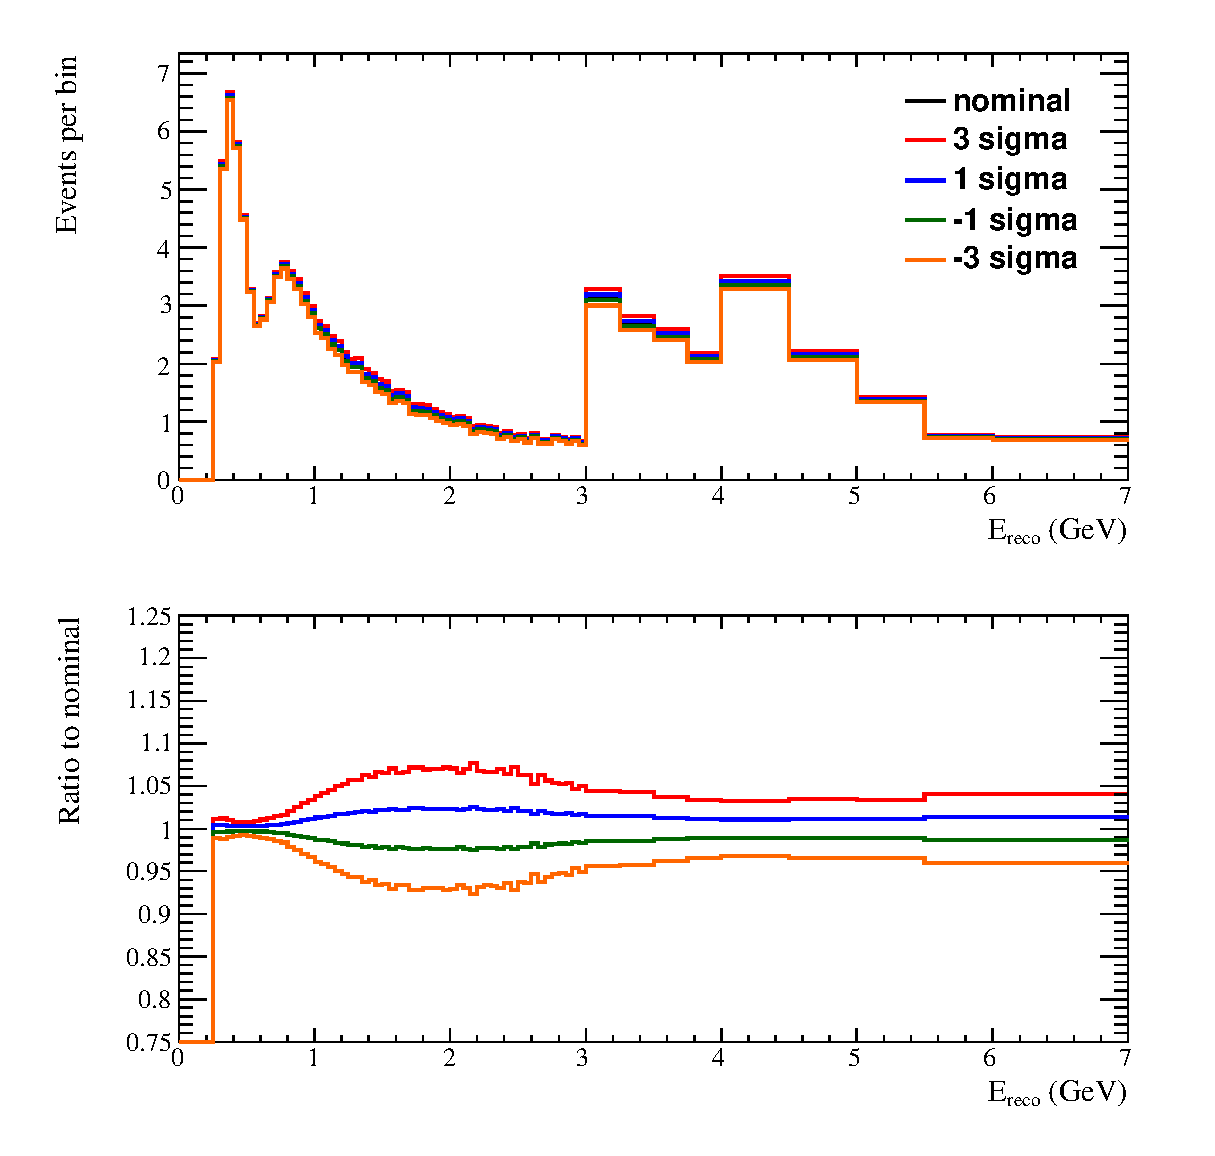
\includegraphics{../images/spectrum_tweaked/1sigma_oscillated/ereco_twk_f_norm_antinutonu}}
\caption
{ Effect of $f_{CC\bar{\nu}; t}$ for 3 flavour oscillations, using oscillation parameters:  $\sin^2\theta_{12} = $0.306; $\sin^2\theta_{13} = $0.0251; $\sin^2\theta_{23} = $0.5; $\delta_{CP} = $        0; $\Delta m^2_{21} = $    7.5e-05 eV$^2$/c$^4$; $|\Delta m^2_{32}| = $    0.0024 eV$^2$/c$^4$. }
\label{fig:osc_ereco_twk_f_norm_antinutonu}
\end{center}
\end{figure}
\clearpage

\begin{figure}
\begin{center}
\resizebox{14cm}{!}{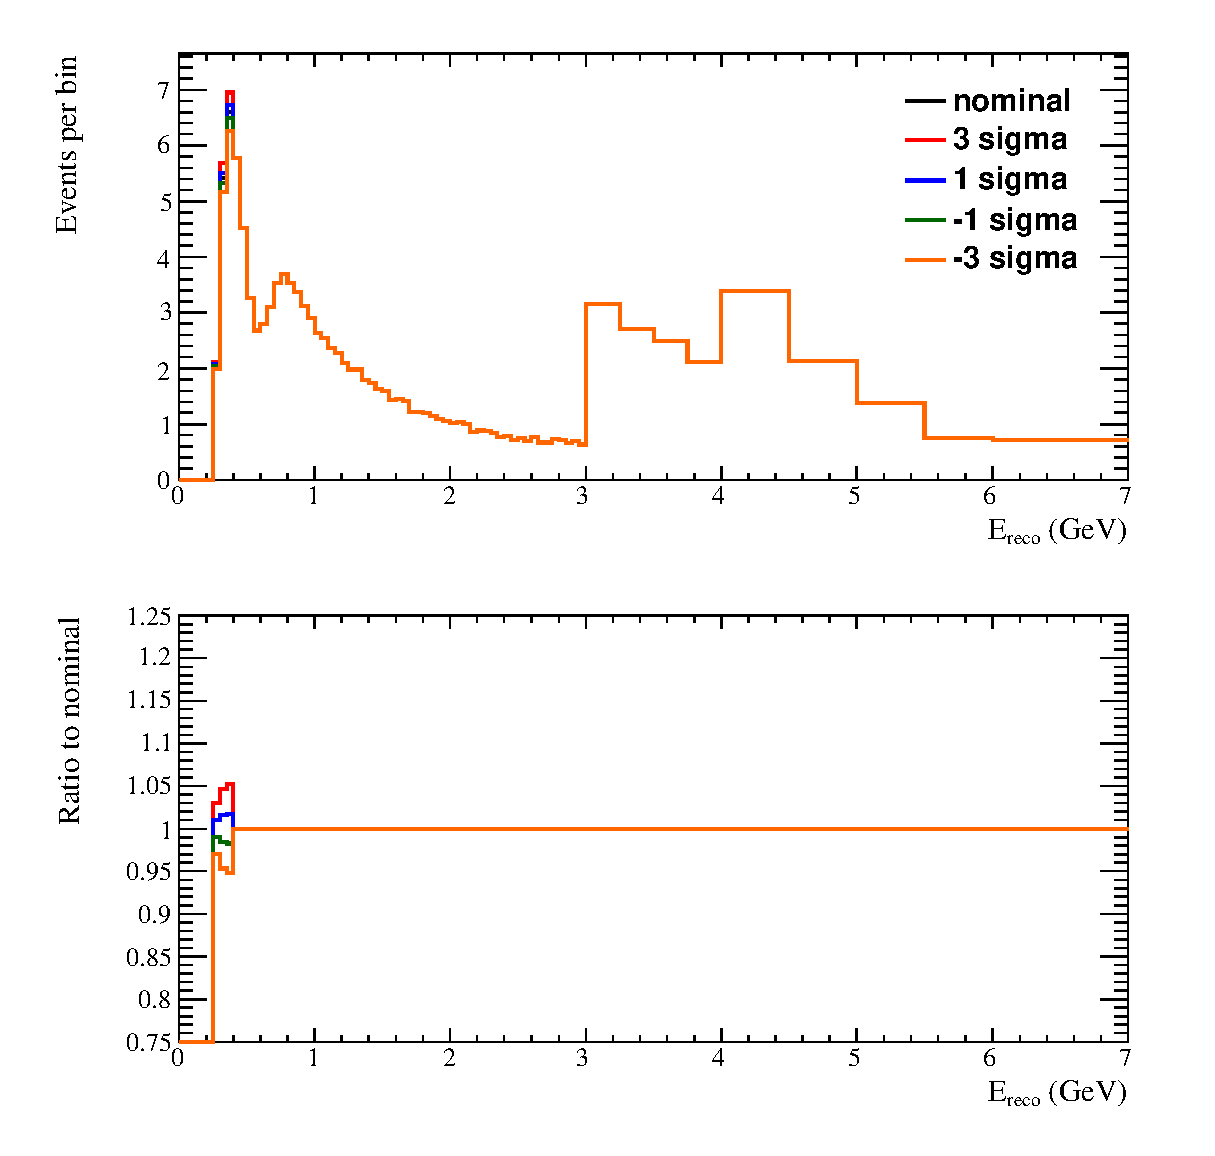
\includegraphics{../images/spectrum_tweaked/1sigma_oscillated/ereco_twk_f_skdetfsi000}}
\caption
{ Effect of $f_{0; r}^{SK+FSI}$ for 3 flavour oscillations, using oscillation parameters:  $\sin^2\theta_{12} = $0.306; $\sin^2\theta_{13} = $0.0251; $\sin^2\theta_{23} = $0.5; $\delta_{CP} = $        0; $\Delta m^2_{21} = $    7.5e-05 eV$^2$/c$^4$; $|\Delta m^2_{32}| = $    0.0024 eV$^2$/c$^4$. }
\label{fig:osc_ereco_twk_f_skdetfsi000}
\end{center}
\end{figure}
\clearpage

\begin{figure}
\begin{center}
\resizebox{14cm}{!}{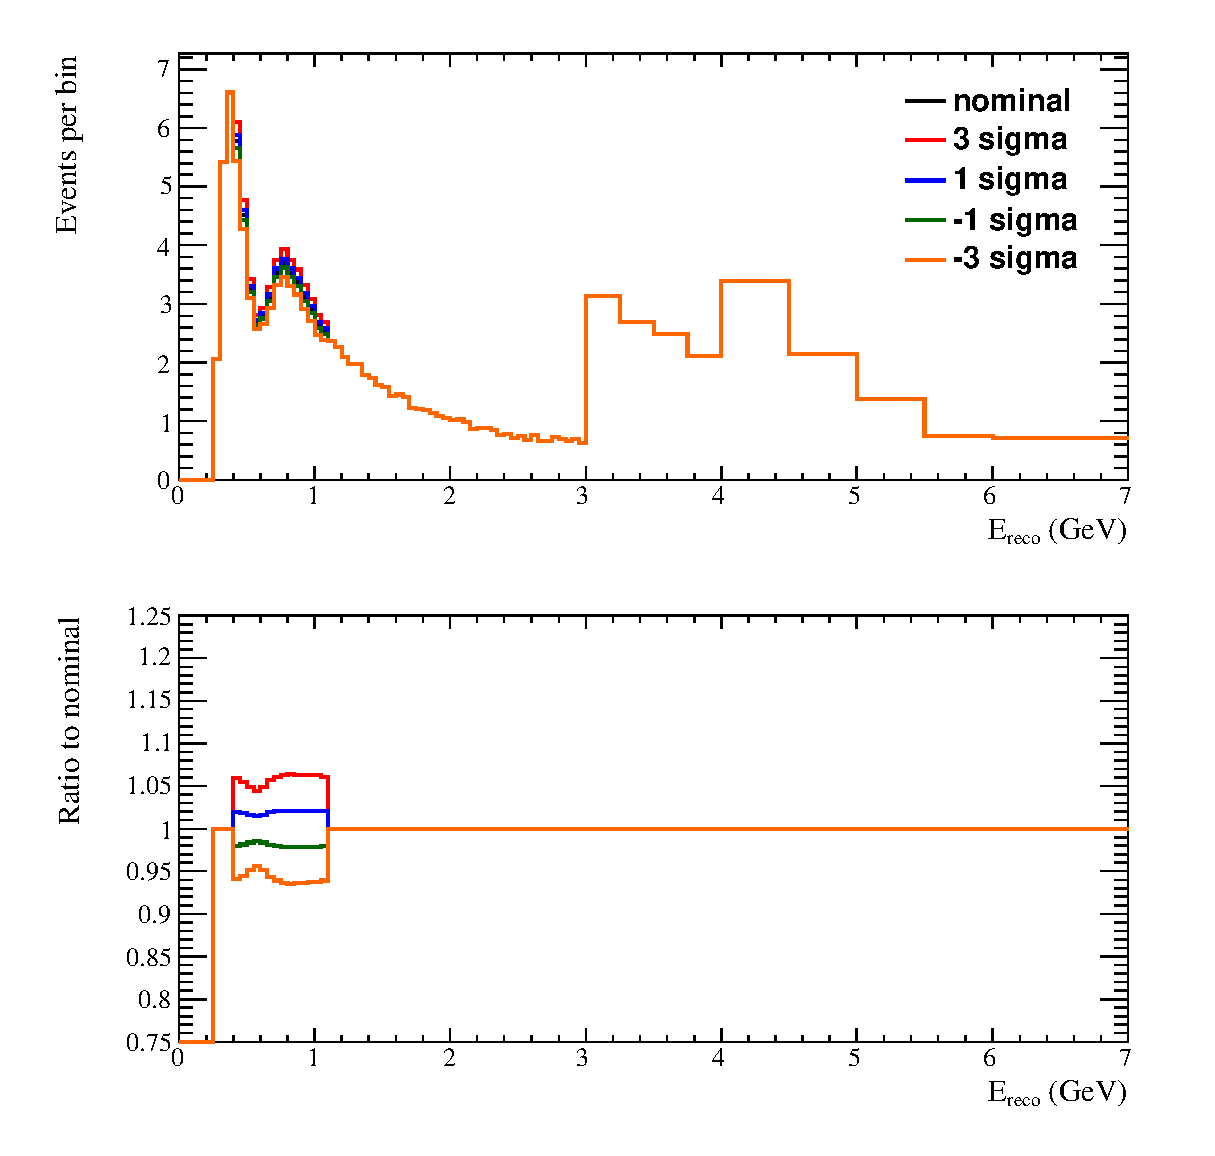
\includegraphics{../images/spectrum_tweaked/1sigma_oscillated/ereco_twk_f_skdetfsi001}}
\caption
{ Effect of $f_{1; r}^{SK+FSI}$ for 3 flavour oscillations, using oscillation parameters:  $\sin^2\theta_{12} = $0.306; $\sin^2\theta_{13} = $0.0251; $\sin^2\theta_{23} = $0.5; $\delta_{CP} = $        0; $\Delta m^2_{21} = $    7.5e-05 eV$^2$/c$^4$; $|\Delta m^2_{32}| = $    0.0024 eV$^2$/c$^4$. }
\label{fig:osc_ereco_twk_f_skdetfsi001}
\end{center}
\end{figure}
\clearpage

\begin{figure}
\begin{center}
\resizebox{14cm}{!}{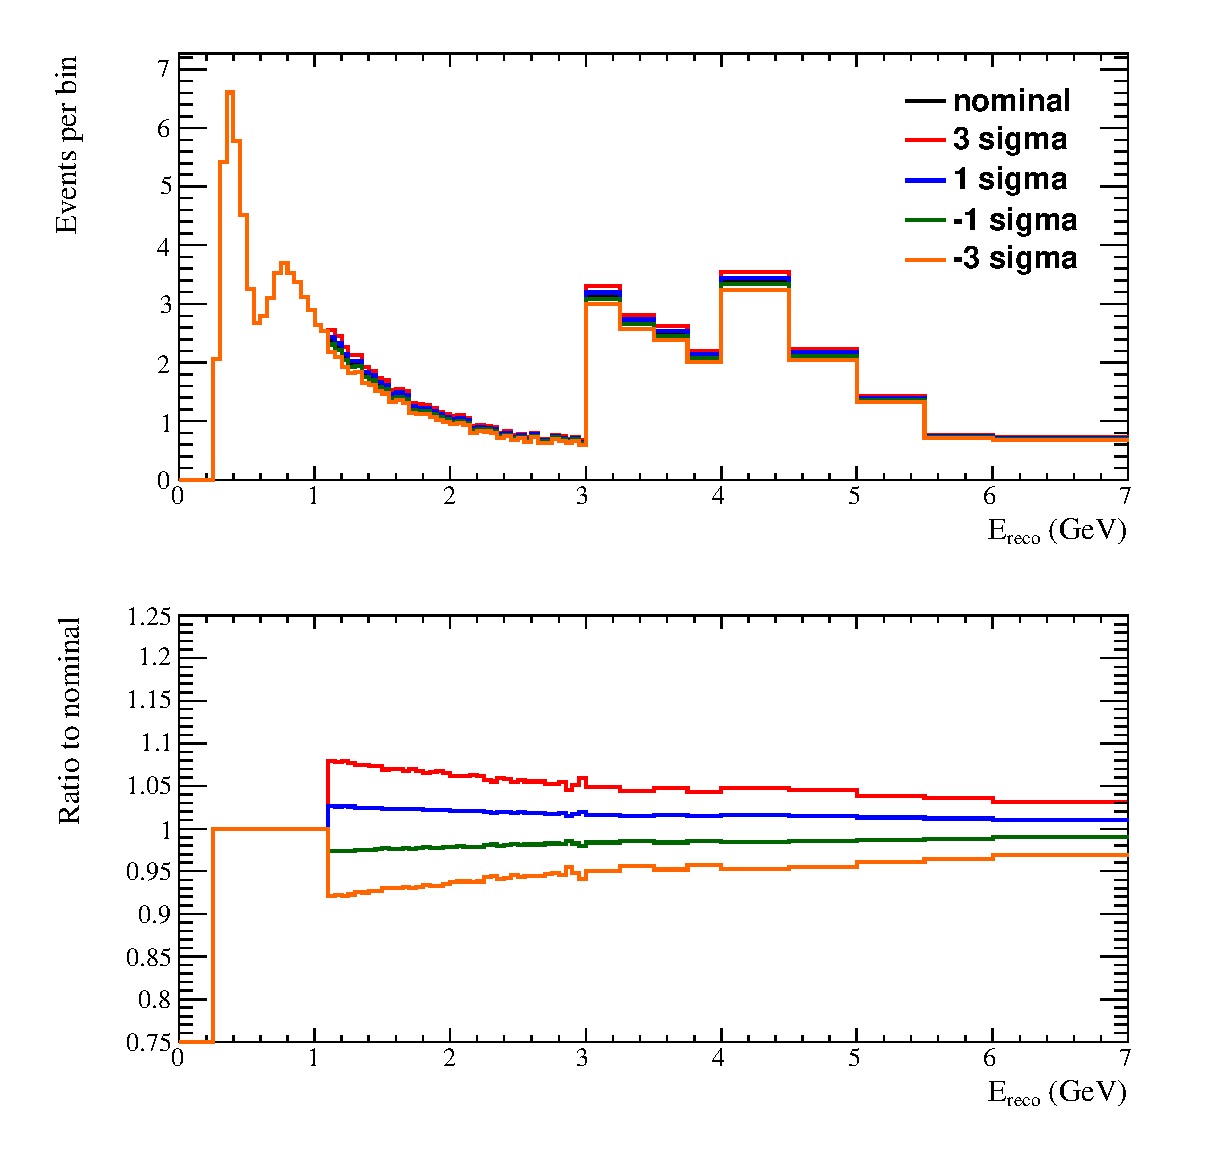
\includegraphics{../images/spectrum_tweaked/1sigma_oscillated/ereco_twk_f_skdetfsi002}}
\caption
{ Effect of $f_{2; r}^{SK+FSI}$ for 3 flavour oscillations, using oscillation parameters:  $\sin^2\theta_{12} = $0.306; $\sin^2\theta_{13} = $0.0251; $\sin^2\theta_{23} = $0.5; $\delta_{CP} = $        0; $\Delta m^2_{21} = $    7.5e-05 eV$^2$/c$^4$; $|\Delta m^2_{32}| = $    0.0024 eV$^2$/c$^4$. }
\label{fig:osc_ereco_twk_f_skdetfsi002}
\end{center}
\end{figure}
\clearpage

\begin{figure}
\begin{center}
\resizebox{14cm}{!}{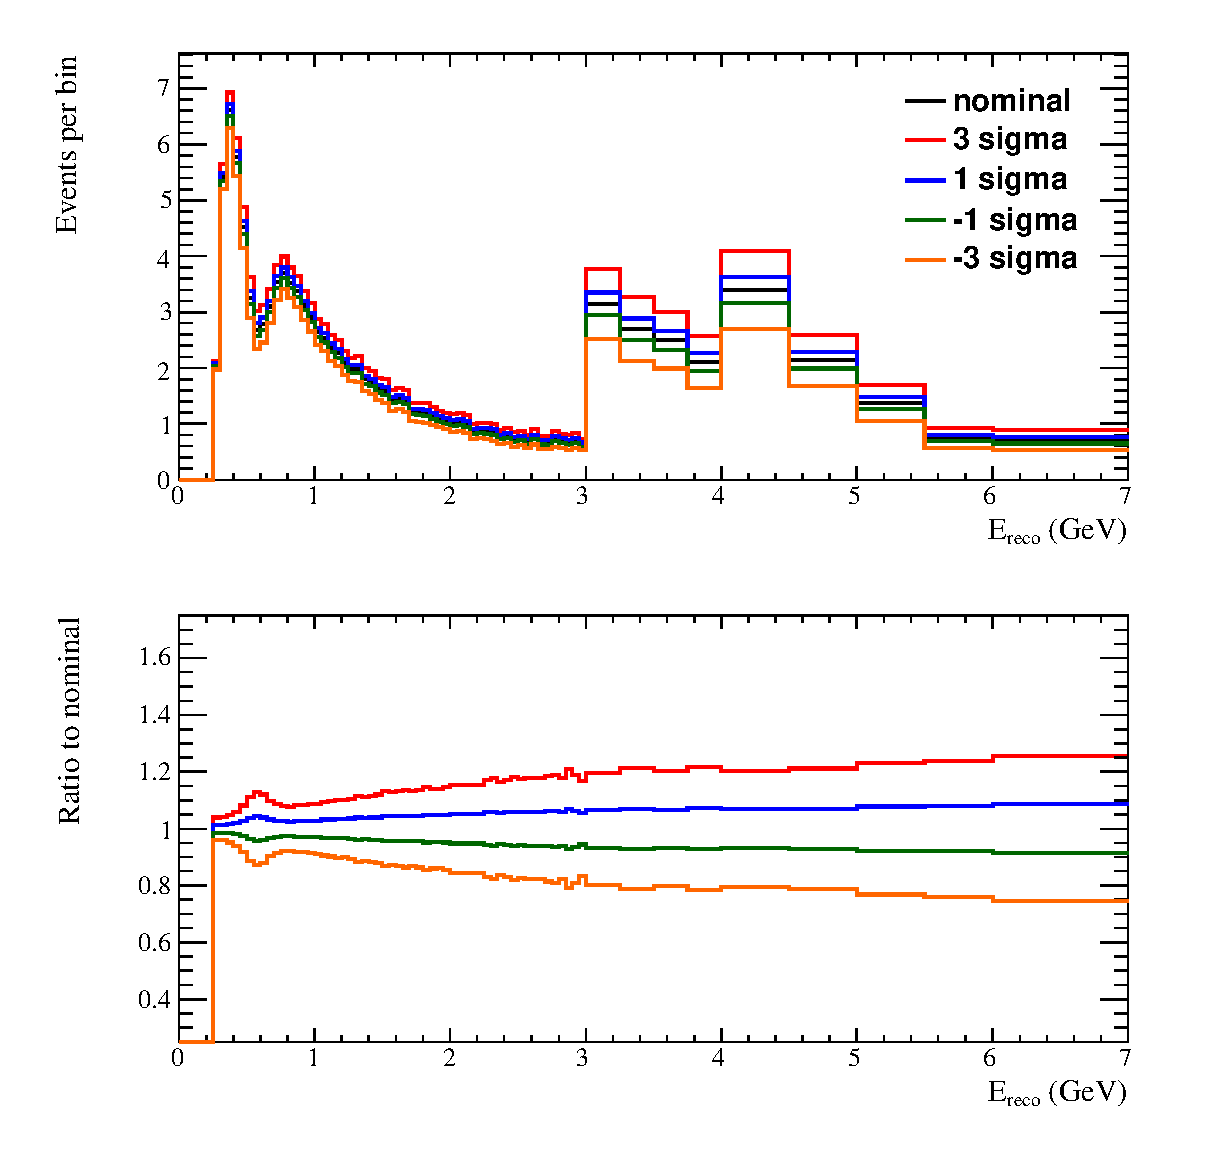
\includegraphics{../images/spectrum_tweaked/1sigma_oscillated/ereco_twk_f_skdetfsi003}}
\caption
{ Effect of $f_{3; r}^{SK+FSI}$ for 3 flavour oscillations, using oscillation parameters:  $\sin^2\theta_{12} = $0.306; $\sin^2\theta_{13} = $0.0251; $\sin^2\theta_{23} = $0.5; $\delta_{CP} = $        0; $\Delta m^2_{21} = $    7.5e-05 eV$^2$/c$^4$; $|\Delta m^2_{32}| = $    0.0024 eV$^2$/c$^4$. }
\label{fig:osc_ereco_twk_f_skdetfsi003}
\end{center}
\end{figure}
\clearpage

\begin{figure}
\begin{center}
\resizebox{14cm}{!}{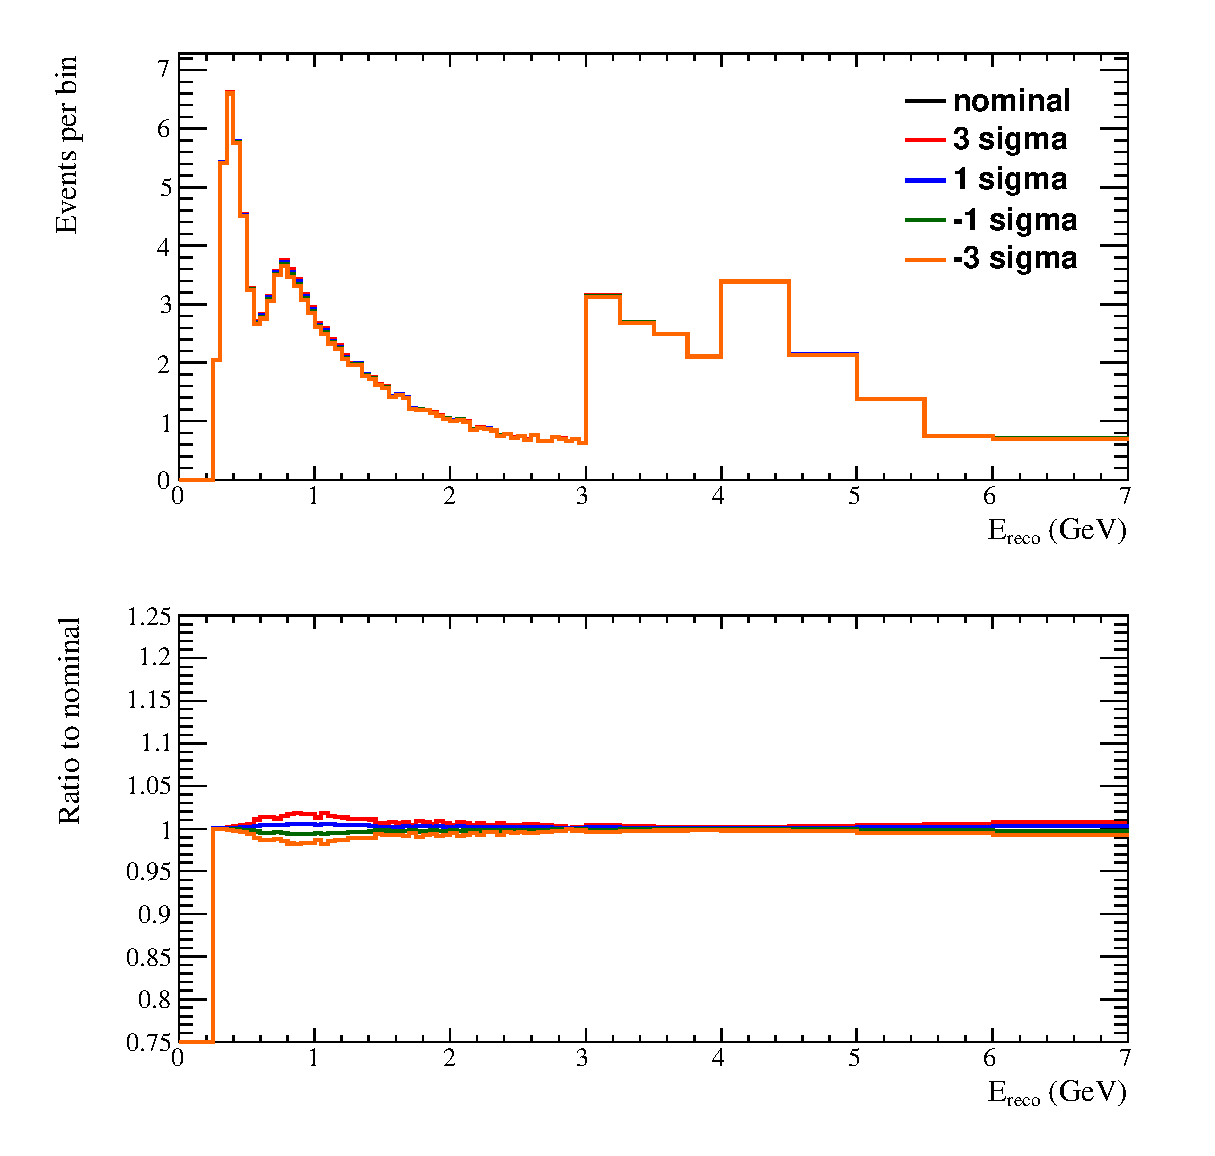
\includegraphics{../images/spectrum_tweaked/1sigma_oscillated/ereco_twk_f_skdetfsi004}}
\caption
{ Effect of $f_{4; r}^{SK+FSI}$ for 3 flavour oscillations, using oscillation parameters:  $\sin^2\theta_{12} = $0.306; $\sin^2\theta_{13} = $0.0251; $\sin^2\theta_{23} = $0.5; $\delta_{CP} = $        0; $\Delta m^2_{21} = $    7.5e-05 eV$^2$/c$^4$; $|\Delta m^2_{32}| = $    0.0024 eV$^2$/c$^4$. }
\label{fig:osc_ereco_twk_f_skdetfsi004}
\end{center}
\end{figure}
\clearpage

\begin{figure}
\begin{center}
\resizebox{14cm}{!}{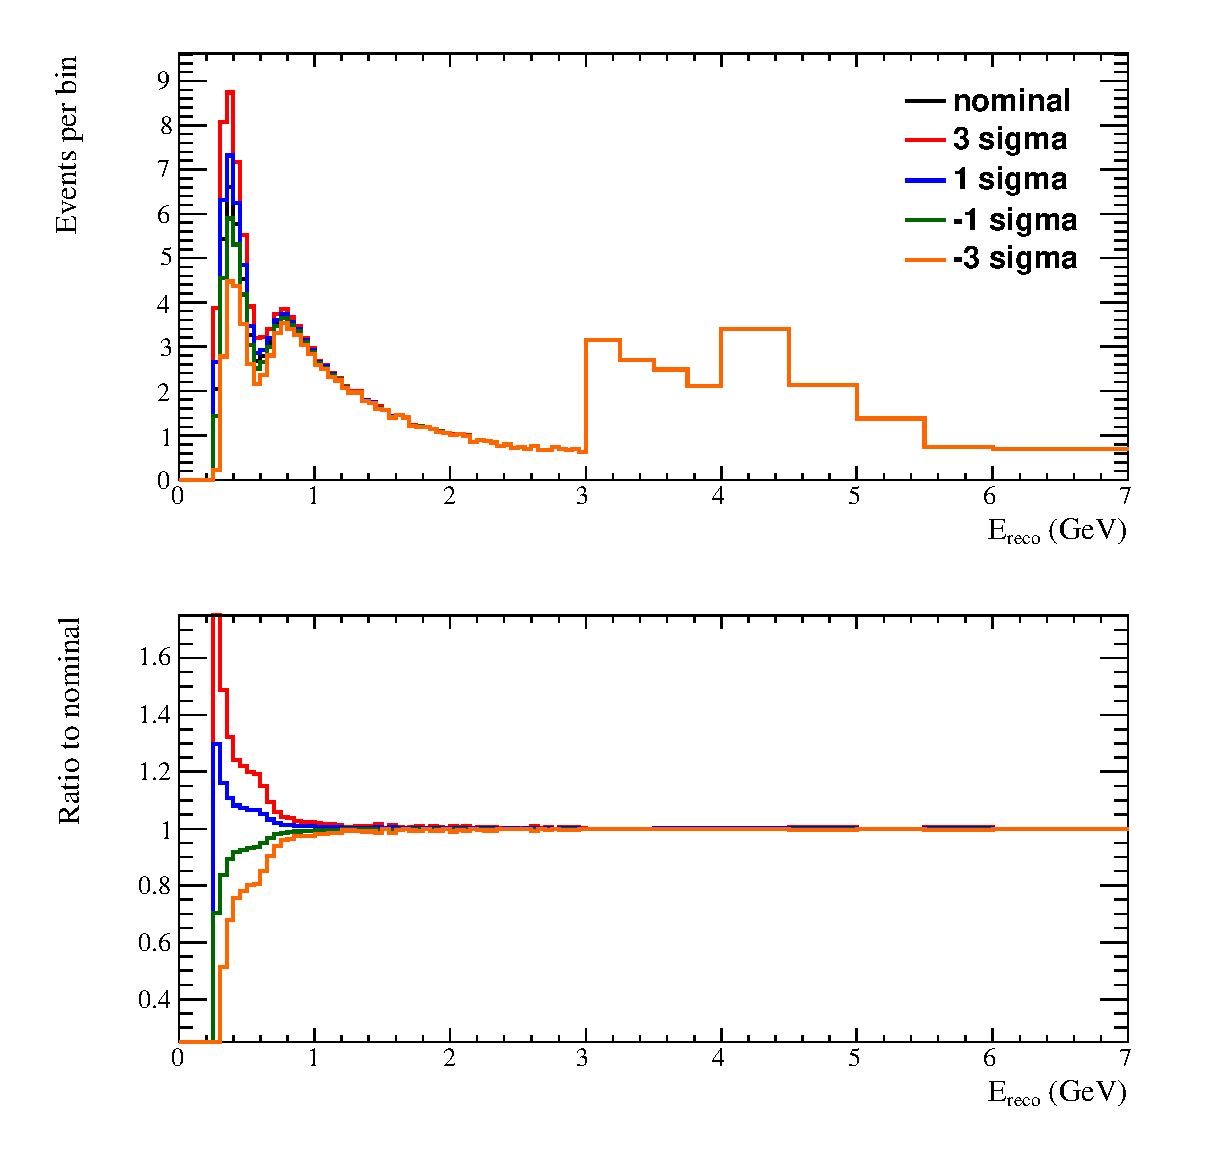
\includegraphics{../images/spectrum_tweaked/1sigma_oscillated/ereco_twk_f_skdetfsi005}}
\caption
{ Effect of $f_{5; r}^{SK+FSI}$ for 3 flavour oscillations, using oscillation parameters:  $\sin^2\theta_{12} = $0.306; $\sin^2\theta_{13} = $0.0251; $\sin^2\theta_{23} = $0.5; $\delta_{CP} = $        0; $\Delta m^2_{21} = $    7.5e-05 eV$^2$/c$^4$; $|\Delta m^2_{32}| = $    0.0024 eV$^2$/c$^4$. }
\label{fig:osc_ereco_twk_f_skdetfsi005}
\end{center}
\end{figure}
\clearpage







\clearpage

\section{SuperK MC templates}
\label{sec:mc_templates}

The nominal SuperK MC templates
are shown in Figs. \ref{fig:etrue_ereco_templates:numu}-\ref{fig:etrue_ereco_templates:oscnue}.
They are shown in the binning used for the analysis, which is
84 true energy bins:
\begin{itemize}
\item   6 50-MeV bins from 0-0.3 GeV; 
\item   28 25-MeV bins from 0.3-1 GeV; 
\item   40 50-MeV bins from 1-3 GeV; 
\item   5 100-MeV bin from 3-3.5 GeV; 
\item   1 bin from 3.5-4 GeV; 
\item   1 bin from 4-5 GeV; 
\item   1 bin from 5-7 GeV; 
\item   1 bin from 7-10 GeV;
\item   1 bin from 10-30 GeV,
\end{itemize}
and 73 reconstructed energy bins:
\begin{itemize}
\item   60 50-MeV bins from 0-3 GeV; 
\item   4 250-MeV bins from 3-4 GeV; 
\item   4 500-MeV bins from 4-6 GeV; 
\item   4 1000-MeV bins from 6-10 GeV;
\item   1 bin from 10-30 GeV.
\end{itemize}

%
% Figs for \subsection{SuperK MC templates in the chosen binning}
%

\begin{figure*}[htb]
\center
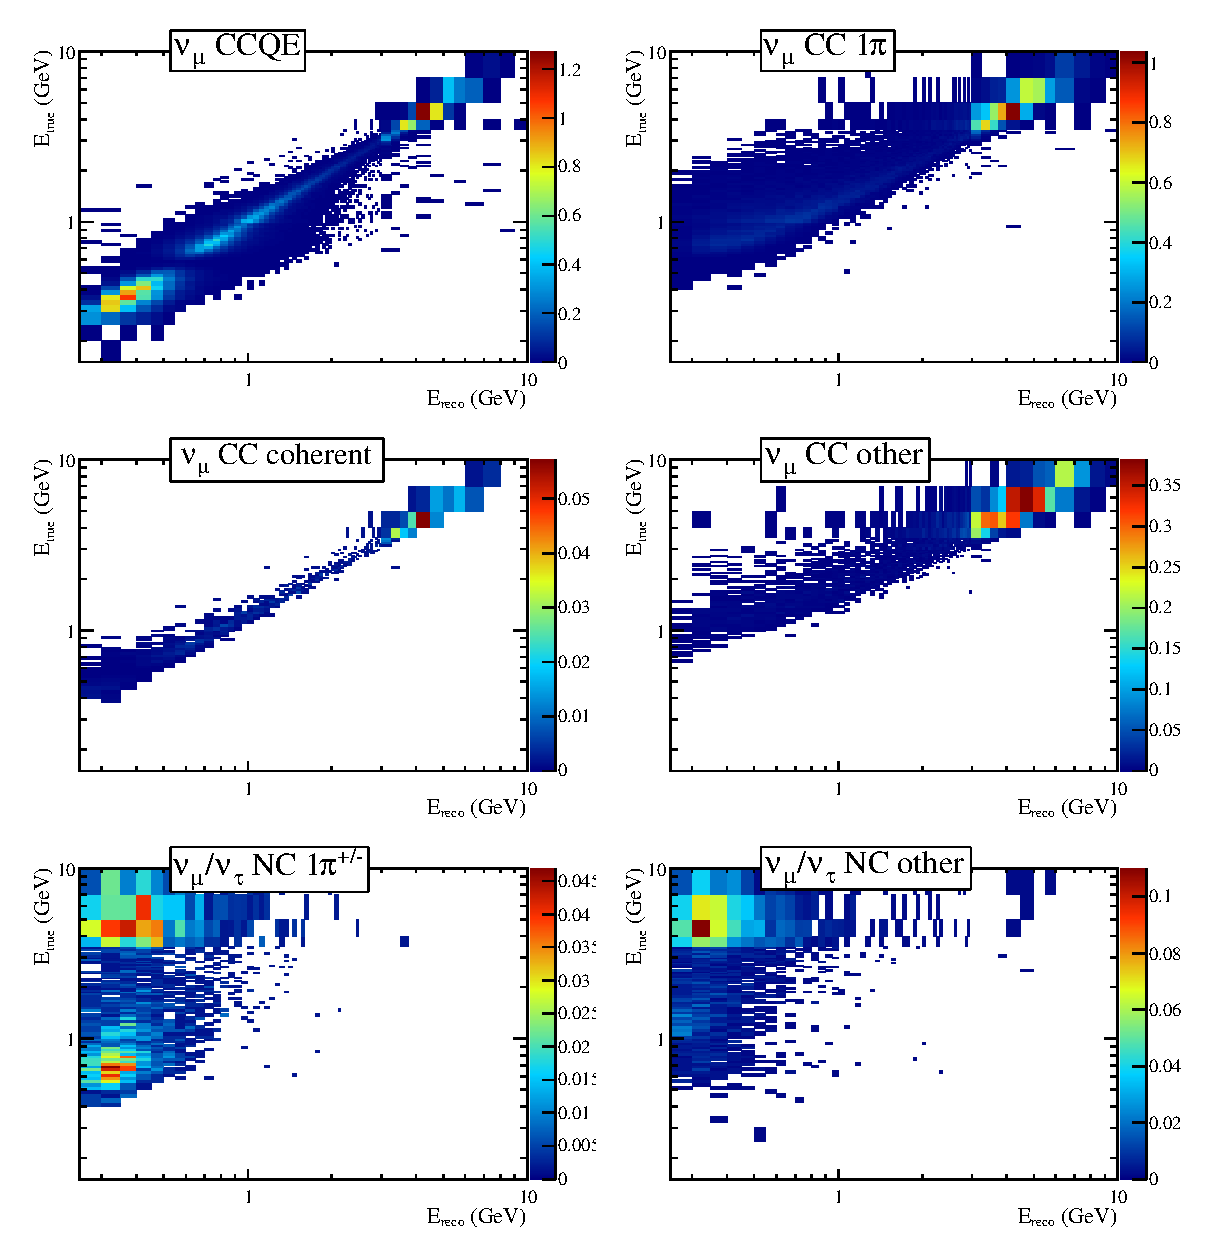
\includegraphics[width=35pc]{../images/templates/mc_template_0}
\caption{
  Nominal ($E_{t}$, $E_{r}$) 1-ring $\mu$-like MC templates. 
  The templates are shown for
  $\nu_{\mu}$ CCQE
  $\nu_{\mu}$ CC1$\pi$, 
  $\nu_{\mu}$ CC coherent, 
  $\nu_{\mu}$ CC other, 
  $\nu_{\mu}$ NC1$\pi^{\pm}$, 
  $\nu_{\mu}$ NC other.
}
\label{fig:etrue_ereco_templates:numu}
\end{figure*}

\begin{figure*}[htb]
\center
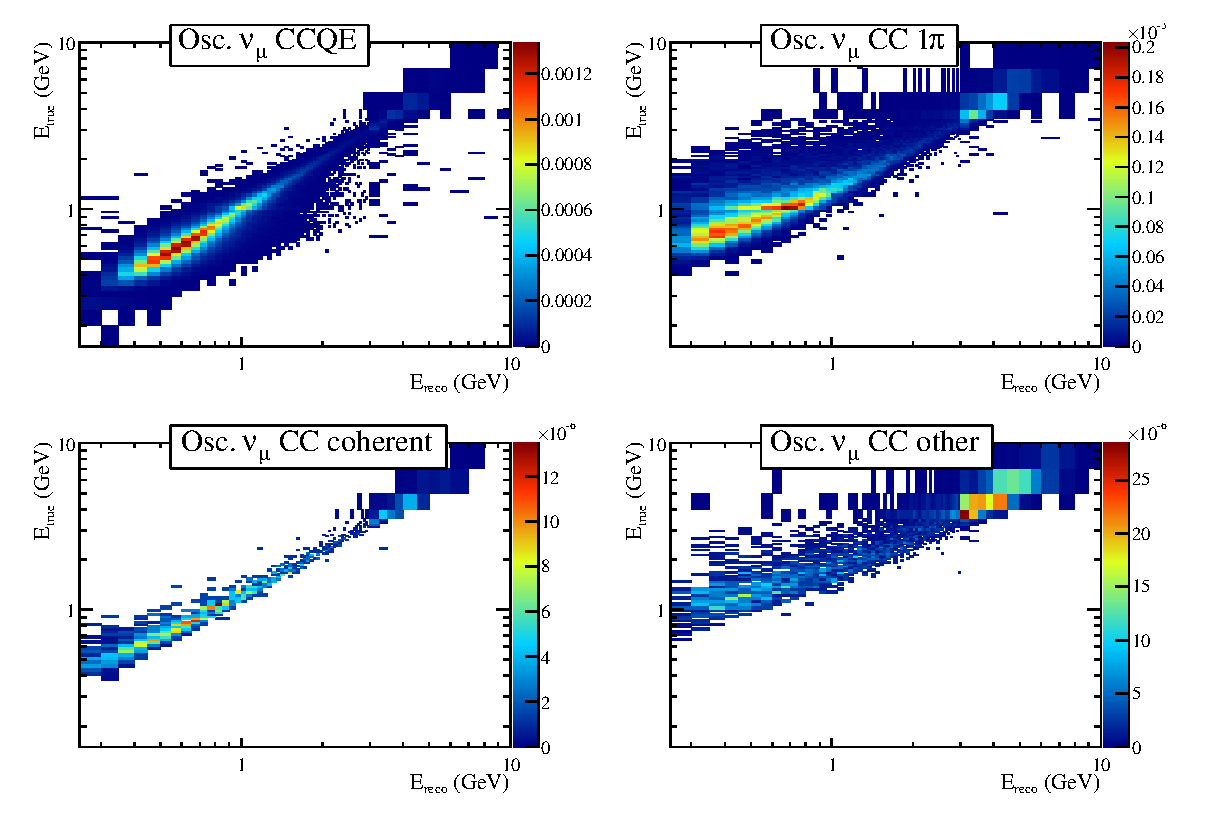
\includegraphics[width=35pc]{../images/templates/mc_template_1}
\caption{
  Nominal ($E_{t}$, $E_{r}$) 1-ring $\mu$-like MC templates. 
  The templates are shown for
  osc. $\nu_{\mu}$ CCQE, 
  osc. $\nu_{\mu}$ CC1$\pi$,
  osc. $\nu_{\mu}$ CC coherent and
  osc. $\nu_{\mu}$ CC other.
}
\label{fig:etrue_ereco_templates:oscnumu}
\end{figure*}

\begin{figure*}[htb]
\center
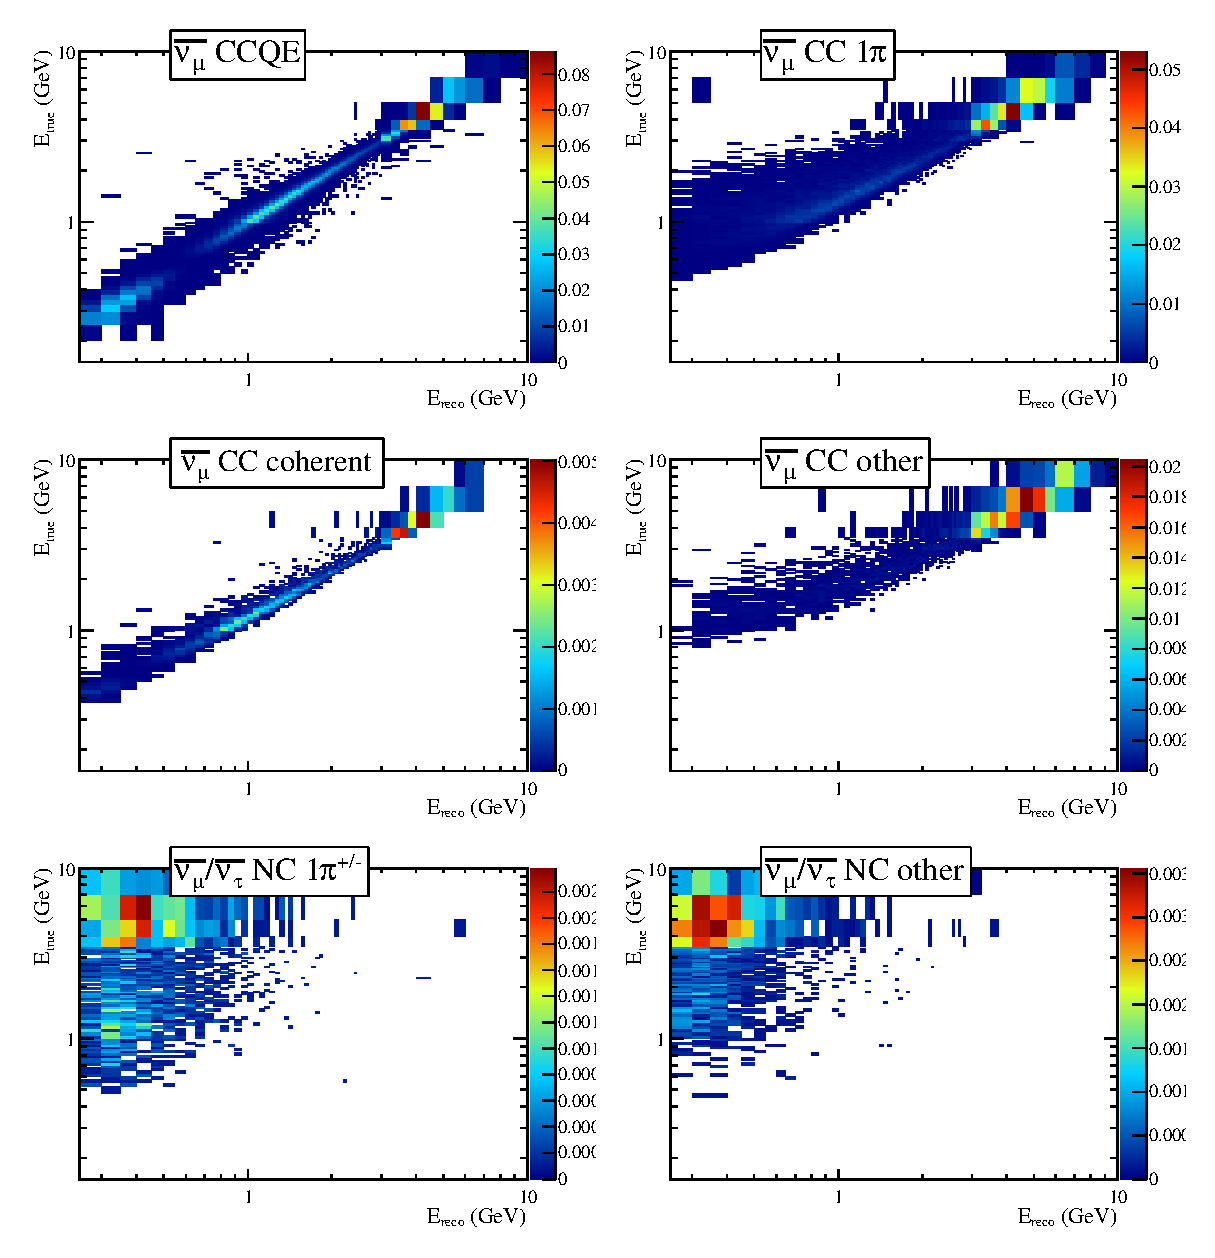
\includegraphics[width=35pc]{../images/templates/mc_template_2}
\caption{
  Nominal ($E_{t}$, $E_{r}$) 1-ring $\mu$-like MC templates. 
  The templates are shown for
  $\bar{\nu_{\mu}}$ CCQE, 
  $\bar{\nu_{\mu}}$ CC1$\pi$, 
  $\bar{\nu_{\mu}}$ CC coherent, 
  $\bar{\nu_{\mu}}$ CC other, 
  $\bar{\nu_{\mu}}$ NC1$\pi^{\pm}$, 
  $\bar{\nu_{\mu}}$ NC other.
}
\label{fig:etrue_ereco_templates:numubar}
\end{figure*}

\begin{figure*}[htb]
\center
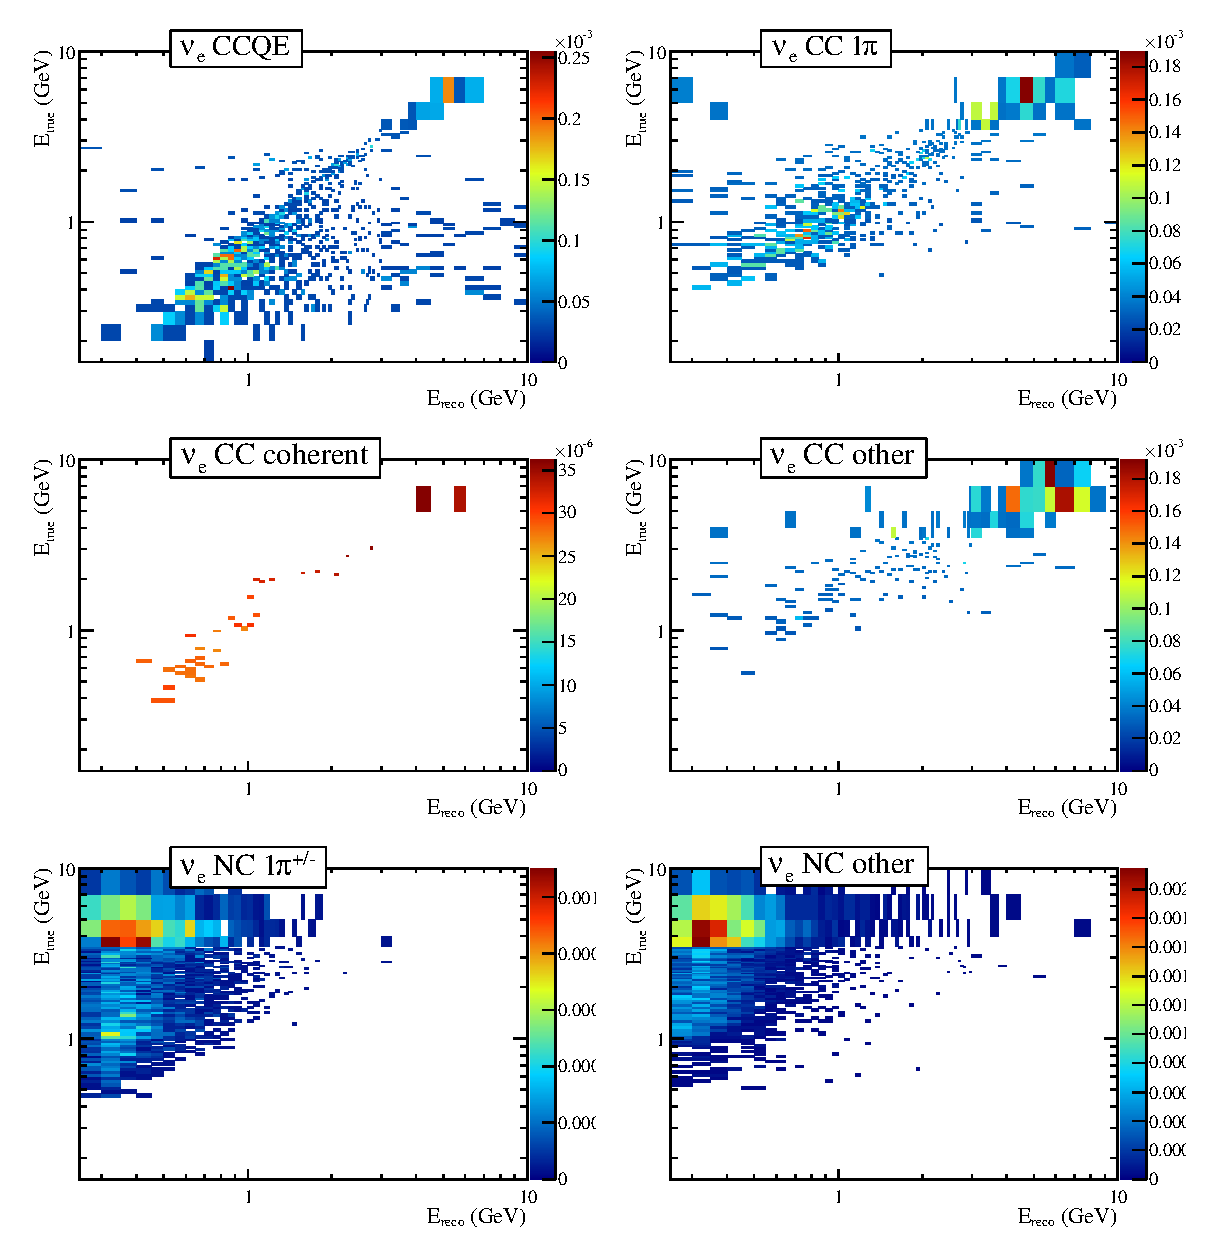
\includegraphics[width=35pc]{../images/templates/mc_template_3}
\caption{
  Nominal ($E_{t}$, $E_{r}$) 1-ring $\mu$-like MC templates. 
  The templates are shown for
  $\nu_{e}$ CCQE, 
  $\nu_{e}$ CC1$\pi$,
  $\nu_{e}$ CC coherent,
  $\nu_{e}$ CC other,
  $\nu_{e}$ NC1$\pi^{\pm}$,
  $\nu_{e}$ NC other.
}
\label{fig:etrue_ereco_templates:nue}
\end{figure*}

\begin{figure*}[htb]
\center
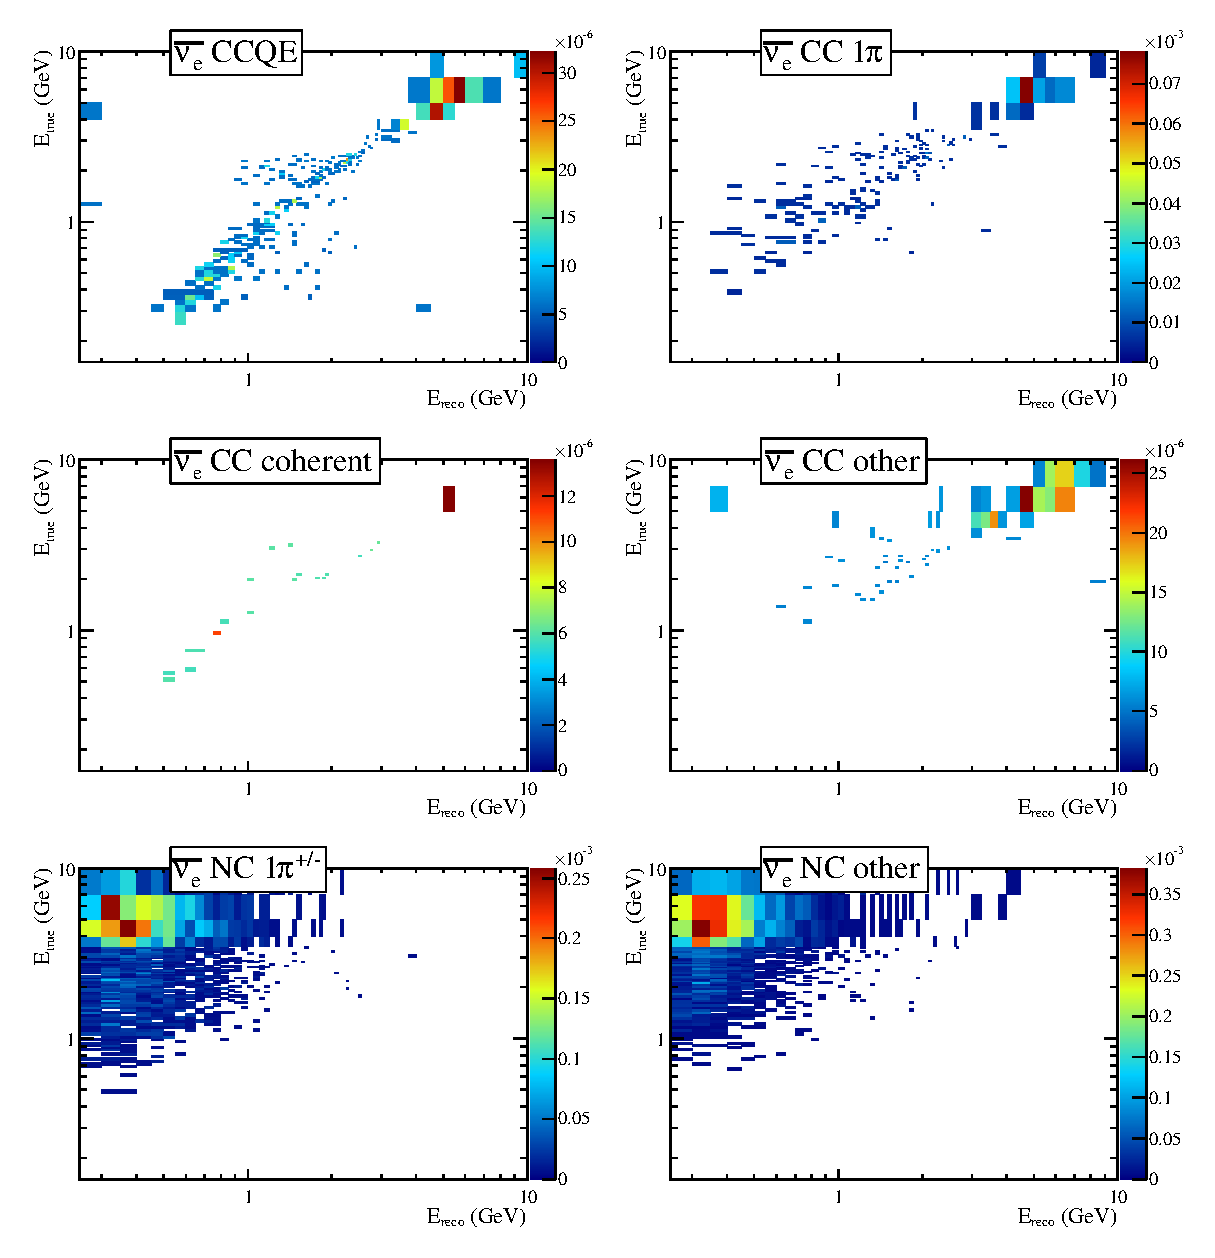
\includegraphics[width=35pc]{../images/templates/mc_template_4}
\caption{
  Nominal ($E_{t}$, $E_{r}$) 1-ring $\mu$-like MC templates. 
  The templates are shown for
  $\bar{\nu_{e}}$ CCQE, 
  $\bar{\nu_{e}}$ CC1$\pi$,
  $\bar{\nu_{e}}$ CC coherent,
  $\bar{\nu_{e}}$ CC other,
  $\bar{\nu_{e}}$ NC1$\pi^{\pm}$,
  $\bar{\nu_{e}}$ NC other.
}
\label{fig:etrue_ereco_templates:nuebar}
\end{figure*}

\begin{figure*}[htb]
\center
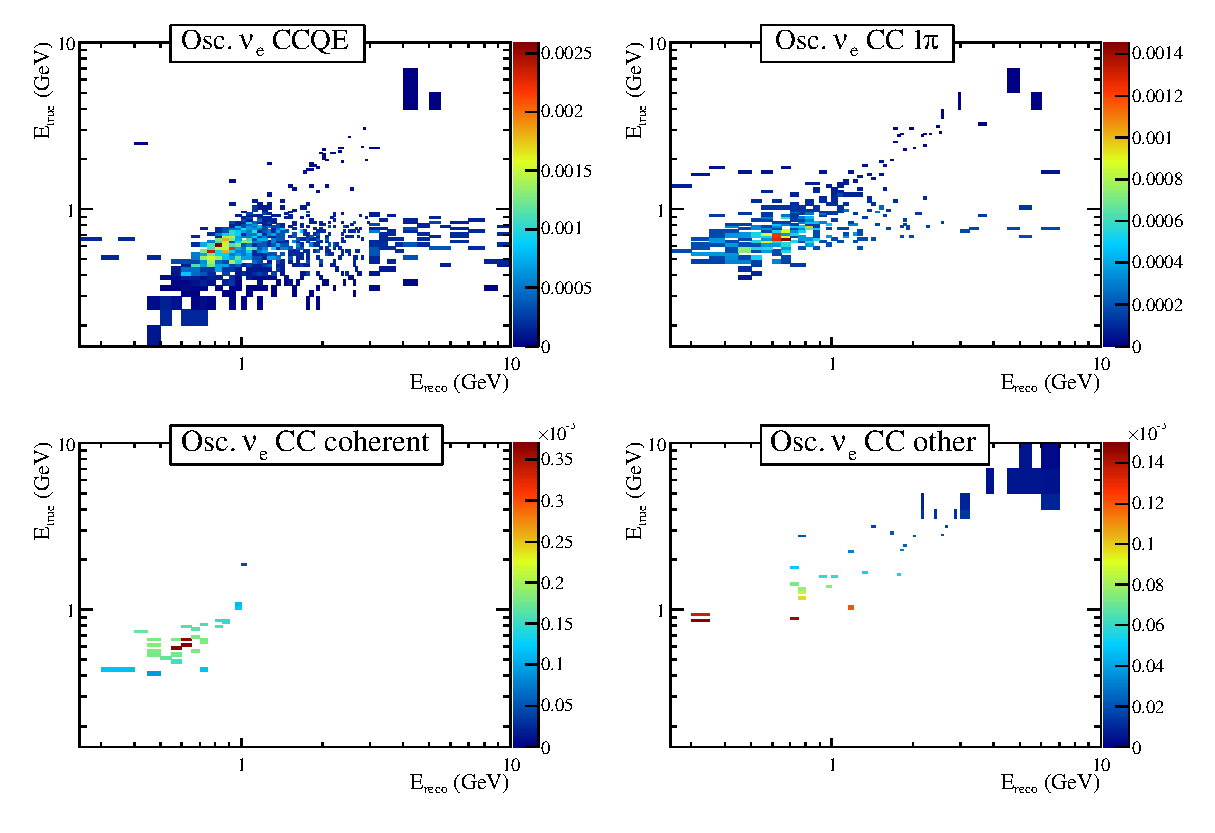
\includegraphics[width=35pc]{../images/templates/mc_template_5}
\caption{
  Nominal ($E_{t}$, $E_{r}$) 1-ring $\mu$-like MC templates. 
  The templates are shown for
  osc. $\nu_{e}$ CCQE, 
  osc. $\nu_{e}$ CC1$\pi$,
  osc. $\nu_{e}$ CC coherent and
  osc. $\nu_{e}$ CC other.
}
\label{fig:etrue_ereco_templates:oscnue}
\end{figure*}



% Appendices
%\clearpage
%\appendix
%\addappheadtotoc
%\clearpage

\end{document}

